\documentclass[mathserif]{beamer}
\usepackage[utf8]{inputenc}
\usepackage{amsmath}
\usepackage{amsfonts}
\usepackage{amssymb}
\usepackage{arydshln}
\usepackage{graphicx}
\usepackage{float}
\usepackage{picture}
\usepackage{dcolumn}
\usepackage{textpos}
\usepackage{graphicx}
\usepackage{subcaption}
\usepackage{tikz}
\usepackage{pgfplots}
\usepackage{listings}
\usepackage{minted}
\setminted{
	framesep=2mm,
	bgcolor=black!5,
	fontsize=\footnotesize,
	linenos,
	obeytabs,
	tabsize=4,
	mathescape = true,
	escapeinside=@@
}


\setbeamercolor{structure}{fg=grey}
\usetheme[sectionpage=progressbar, progressbar=frametitle]{metropolis}

\definecolor{prettyBlue}{HTML}{2196F3}
\setbeamercolor{progress bar}{fg=prettyBlue, bg=gray}

%Information to be included in the title page:
\title{Development of a Pendulum Control System}
\author{Thomas S. Christensen \\ Mikkel S. Jaedicke\\}

\institute{University of Southern Denmark}
\date{Jan, 2018} 

\addtobeamertemplate{frametitle}{}{%
\begin{textblock*}{200mm}(\textwidth-1.5cm,-0.8cm)

\includegraphics[scale=0.15]{graphics/sdu_logo}
\end{textblock*}}

\begin{document}

\begin{frame}[t]\frametitle{~}
\maketitle
\end{frame}
\note{Mikkel:
Hej og velkommen på dansk. Glade for at se så mange mennesker. Vi vil fortælle ca. 30 minutter om vores projekt på engelsk.
Derefter sarter vores individuelle eksamen, som vil være lukket for tilhørere.
Efter det hele er oversået vil vi gerne invitere jer alle på et stykke kage og et glas boblevand.
Hi and Welcome to our master thesis exam. We will do a presentation about our project for the next half hour and then the exam will begin and you will be asked to leave.
After the exam is finished we would to invite you all to join our celebration.
Thank you all for coming. }

\begin{frame}[c]\frametitle{Introduction}
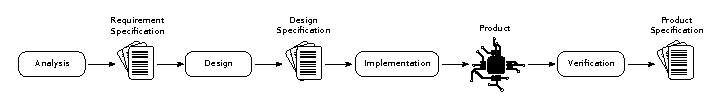
\includegraphics[width=\textwidth]{graphics/workflow}
\vfill
	\begin{columns}
		\begin{column}[c]{.5\textwidth}
			\begin{itemize}
				\item \alert<1>{Analysis}
				\item \alert<2>{Design}
			\end{itemize}
		\end{column}
		\begin{column}[c]{.5\textwidth}
			\begin{itemize}
				\item \alert<3>{Implementation}
				\item \alert<4>{Verification}
			\end{itemize}
		\end{column}
	\end{columns}
	\vspace{0.5cm}
	\hrule
	\vspace{0.4cm}
	\begin{columns}
		\begin{column}[c]{.5\textwidth}
			\begin{itemize}
				\item<5> \alert<5>{Conclusion}
			\end{itemize}
		\end{column}
		\begin{column}[c]{.5\textwidth}
			\begin{itemize}
				\item[~]
			\end{itemize}
		\end{column}
	\end{columns}
\end{frame}
\note{Thomas: Analysis, Design}
\note{Mikkel: Implementation, Verification, Conclusion}
\section{Analysis}

\begin{frame}[c]\frametitle{Analysis - Teaching Underactuated Systems}
	\begin{columns}
		\begin{column}[c]{.5\textwidth}
			\begin{itemize}[<+- | alert@+>]
				\item What is an underactuated system?
				\item Pendulum systems.
				\item Double pendulum system.
			\end{itemize}
		\end{column}
		\begin{column}[c]{.5\textwidth}
			\centering
			\includegraphics<1>[width=\linewidth]{graphics/robo_underactuated}\\
			\vspace{1cm}
			\includegraphics<1>[width=.50\linewidth]{graphics/robo_underactuated_picture}
			\includegraphics<2>[width=\linewidth]{graphics/segway}
			\includegraphics<3>[width=\linewidth]{graphics/joint_assembly.eps}
		\end{column}
	\end{columns}
\end{frame}
\note{Thomas}

\begin{frame}[c]\frametitle{System Overview}
\centering
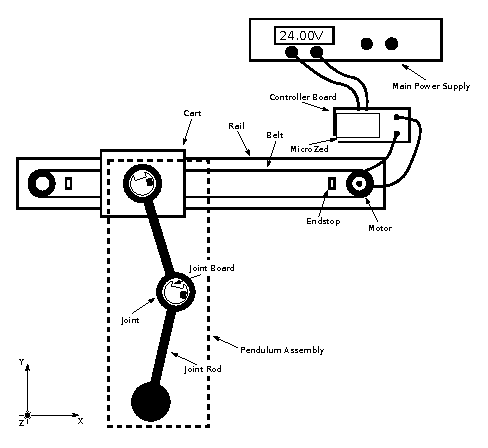
\includegraphics[scale=1]{graphics/system_overview}
\end{frame}
\note{Here we see a full overview of the system.
We see the pendulum assembly attached to a cart.
The cart can be actuated by the motor through the use of the belt.
A controllerboard is used to control the motor and it is powered by a power supply.
There is a small PCB in the joint called the joint board, which transmits data to the controllerboard..}

\begin{frame}[c]\frametitle{Implemented System}
\centering
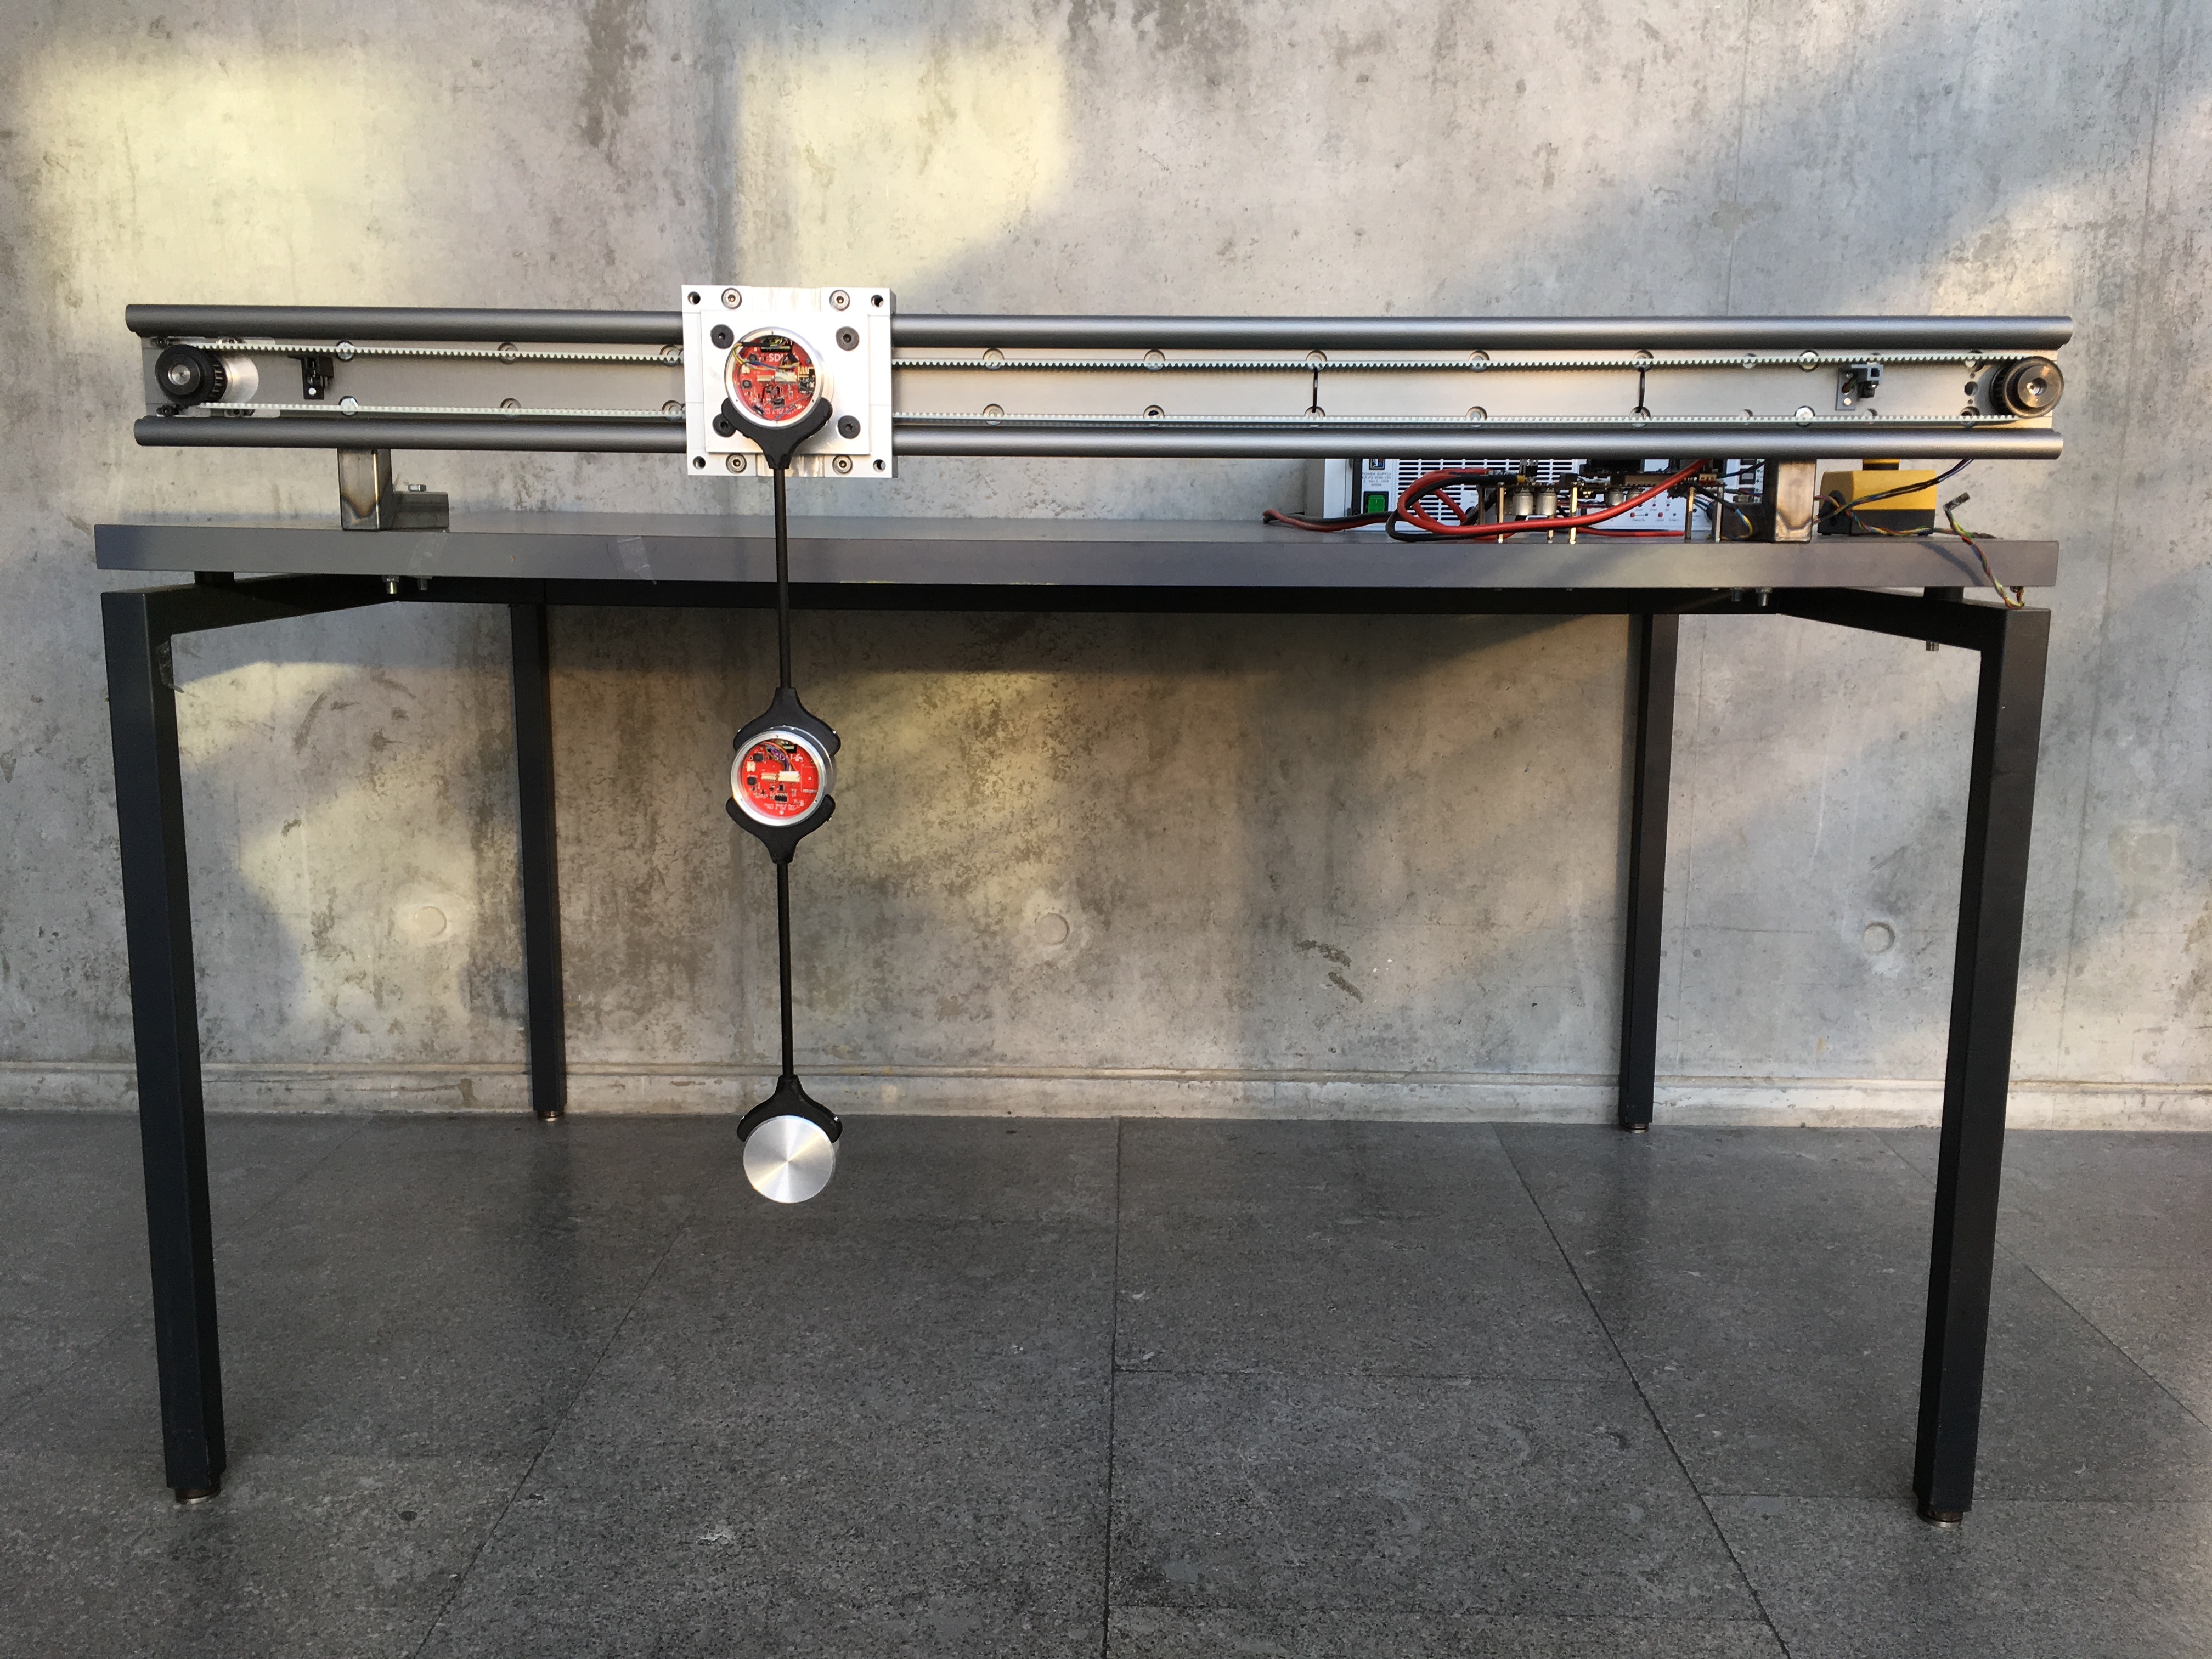
\includegraphics[width=0.9\textwidth]{graphics/full_system_finish}
\end{frame}
\note{Here is the implemented full systems. The rail and belt are seen here. also the motor and the pendulum assembly is easy to spot}

\begin{frame}[c]\frametitle{Requirement Specification}

\textbf{Functional:}
\begin{enumerate}
	\item System should consists of a double pendulum mounted on a moveable cart.\pause
	\item Cart should be actuated by the Maxon 148867. \pause
	\item The pendulum system should be controlled by a MicroZed.\pause
	\item \alert{Position of the cart and joint angles should be measured.}
\end{enumerate}

\end{frame}
\note{Thomas}


\section{Design}

\begin{frame}{Mechanical Design}
	\begin{figure}
	\centering
	\begin{subfigure}{.5\textwidth}
	  \centering
	  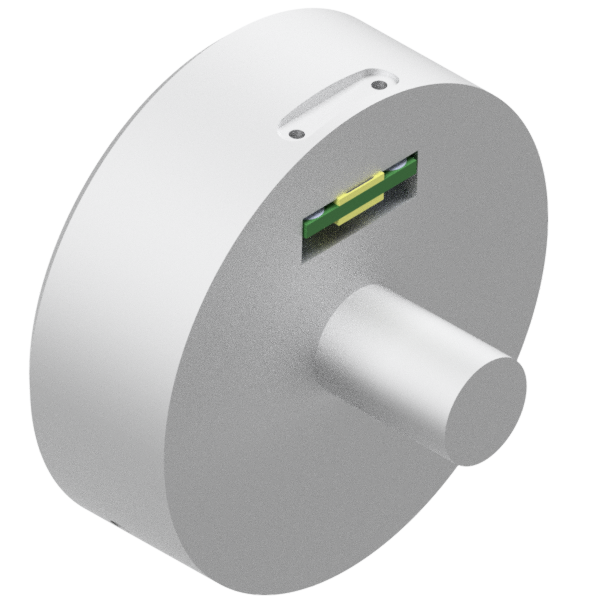
\includegraphics[width=.9\linewidth]{graphics/joint_read_side}
	\end{subfigure}%
	\begin{subfigure}{.5\textwidth}
	  \centering
	  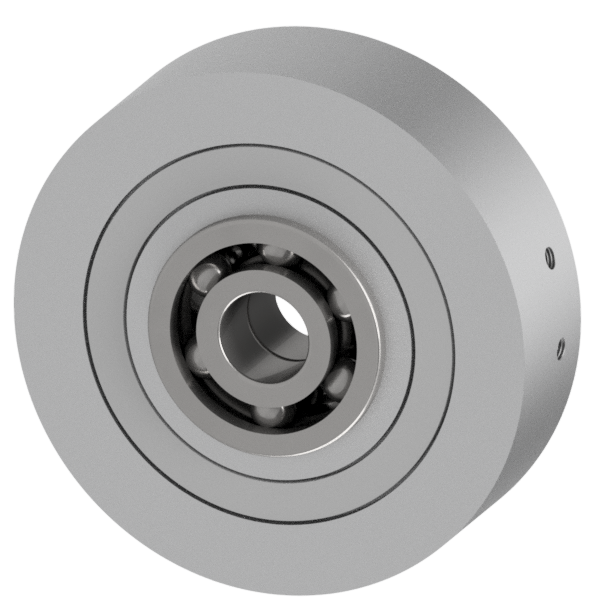
\includegraphics[width=.9\linewidth]{graphics/joint_mag_assembly}
	\end{subfigure}
	\end{figure}
\end{frame}
\note{Thomas}

\begin{frame}[c]\frametitle{Electrical Design}
\textbf{Joint Board:}
	\begin{itemize}
    	\item Encoder
    	\pause
    	\item Wireless Communication
    	\pause
    	\item Microcontroller
    	\pause
    	\item Power Delivery
    \end{itemize}    
\end{frame}
\note{
Encoder - wiring, RS422 conversion IC
Wireless communication - nrf24 module
Microcontroller - ATtiny84
Power delivery -  3.3 v for nrf and ATtiny and 5v for encoder 
}

\begin{frame}[c]\frametitle{Electrical Design}
\textbf{Joint Board:}
	\begin{itemize}
    	\item Encoder
    	\item Wireless Communication
    	\item Microcontroller
    	\item \alert{Power Delivery}
    \end{itemize}    
\end{frame}
\note{Mikkel}

\begin{frame}[c]\frametitle{Power Delivery}
	\centering
	\vfill
    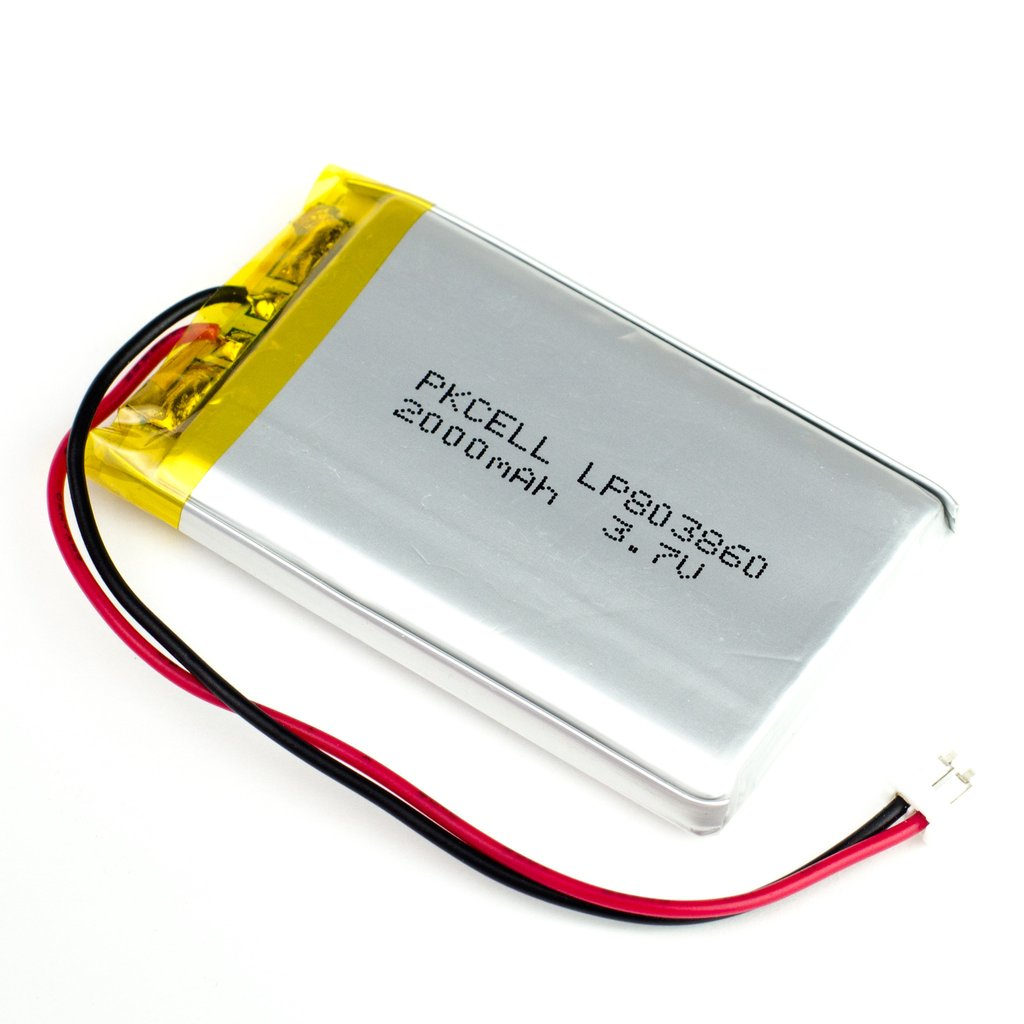
\includegraphics[width=.35\linewidth]{graphics/lipo}\\
    \vfill
    \scalebox{2}{$$3.0V\;\rightarrow\;4.2V \quad\Rightarrow\quad 3.3V$$}
    \vfill
\end{frame}
\note{Classic electronics problem. Battery into stable voltage}

\begin{frame}[c]\frametitle{Power Delivery}
\begin{columns}
\column{.5\linewidth}
\textbf{Solutions:}   
\begin{itemize}
			\item Buck converter
			\item Buck-Boost converter
			\item Linear regulator
\end{itemize}
\column{.5\linewidth}
\textbf{Parameters:}
\begin{itemize}
			\item Efficiency
			\item Drop out voltage
			\item []
\end{itemize}
\end{columns}
\end{frame}
\note{
Buck converter is a Switch mode power supply that uses switching to produce a lower output voltage than input voltage.
Buck-Boost converter is also a Switch mode power supply and has the ability to generate voltages higher and lower than its input voltage.
A linear regulator varies an internal resistance to yield a steady output voltage that is lower than the input voltage.

Two parameters to judge upon:
Efficiency - how much energy is lost in the conversion
Drop out voltage - the voltage that the input voltage needs to be higher than the output voltage
}

\begin{frame}[c]\frametitle{Buck Converter}
	\begin{equation}
		\eta \approx 95\%
	\end{equation}
\pause
	\begin{equation}
		V_{drop} = I_{O} \cdot (R_{DS(on)}+R_I)
		\label{eq:drop_v_tps62}
	\end{equation}
\pause
	\begin{equation}
		V_{drop} = 0.02 \cdot (0.062+0.09) = 14 [mV]
		\label{eq:drop_v_tps62_2}
	\end{equation}
\end{frame}
\note{Drop out voltage in a buck converter is only dependent on the output current and resistance of the output path, which is the resistance ON resistance of the MOSFET and the inductor

The efficiency is found in the datasheet to be 95 percent
}

\begin{frame}[c]\frametitle{Comparison}
	\begin{table}[h]
		\begin{tabular}{l|c|c|c}
			  ~				& \textbf{Buck} 	& \textbf{Buck-Boost}& \textbf{Linear}\tabularnewline 
			 Efficiency  	& 95\% 	& 75\%		& 89\%	\\
			 Drop out [mV]	& 14  	& N/A		& 20	\\
		\end{tabular}
	\end{table}
\end{frame}
\note{Using a buck converter seems to be the best choice. But if it is chosen an amount of the battery capacity cannot be utilized.
}

\begin{frame}[t]\frametitle{Battery Characteristics}
    \begin{figure}[h]
		\centering
		% This file was created by matlab2tikz.
%
%The latest updates can be retrieved from
%  http://www.mathworks.com/matlabcentral/fileexchange/22022-matlab2tikz-matlab2tikz
%where you can also make suggestions and rate matlab2tikz.
%
\definecolor{mycolor1}{rgb}{0.00000,0.44700,0.74100}%
%
\begin{tikzpicture}

\begin{axis}[%
width=4.521in,
height=3.566in,
at={(0.758in,0.481in)},
scale only axis,
xmin=0,
xmax=450,
xlabel style={font=\color{white!15!black}},
xlabel={Time [Min]},
ymin=2.5,
ymax=4.5,
ytick={2.5,   3, 3.5,   4, 4.5},
ylabel style={font=\color{white!15!black}},
ylabel={Voltage [V]},
axis background/.style={fill=white},
title style={font=\bfseries},
title={Discharge Curve of Li-Ion Battery}
]
\addplot [color=mycolor1, forget plot]
  table[row sep=crcr]{%
0	4.072\\
10	4.02699999999999\\
20	4.00799999999998\\
40	3.95999999999998\\
50	3.92200000000003\\
60	3.89499999999998\\
70	3.87900000000002\\
80	3.85500000000002\\
90	3.84300000000002\\
100	3.81799999999998\\
110	3.79700000000003\\
120	3.78899999999999\\
130	3.77699999999999\\
140	3.767\\
150	3.75299999999999\\
160	3.76100000000002\\
170	3.75999999999999\\
180	3.74000000000001\\
190	3.72500000000002\\
200	3.71300000000002\\
210	3.714\\
220	3.69999999999999\\
230	3.71100000000001\\
240	3.71199999999999\\
250	3.69999999999999\\
260	3.69299999999998\\
270	3.69099999999997\\
280	3.69799999999998\\
290	3.69099999999997\\
300	3.68099999999998\\
310	3.673\\
320	3.65699999999998\\
330	3.64499999999998\\
340	3.63499999999999\\
350	3.62299999999999\\
360	3.60700000000003\\
370	3.61399999999998\\
380	3.596\\
390	3.56799999999998\\
400	3.505\\
410	3.36099999999999\\
414.551694551695	2.30000000000001\\
};
\addplot [color=red, dashed, forget plot]
  table[row sep=crcr]{%
0	3.30000000000001\\
450	3.30000000000001\\
};
\end{axis}
\end{tikzpicture}%
	\end{figure}
\end{frame}
\note{It can be seen that the majority of the battery capacity can be utilized. Calculations showed that approximately 99 percent can be utilized.

Thus it was concluded that using a buck converter was the best option.}

\begin{frame}[c]\frametitle{Designed PCB}
	\begin{figure}
	\centering
	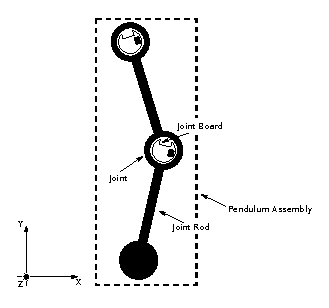
\includegraphics[width=.7\linewidth]{graphics/joint_assembly}
	\end{figure}
\end{frame}
\note{Thomas}

\begin{frame}[c]\frametitle{Designed Pendulum Assembly}
	\begin{figure}
	\centering
	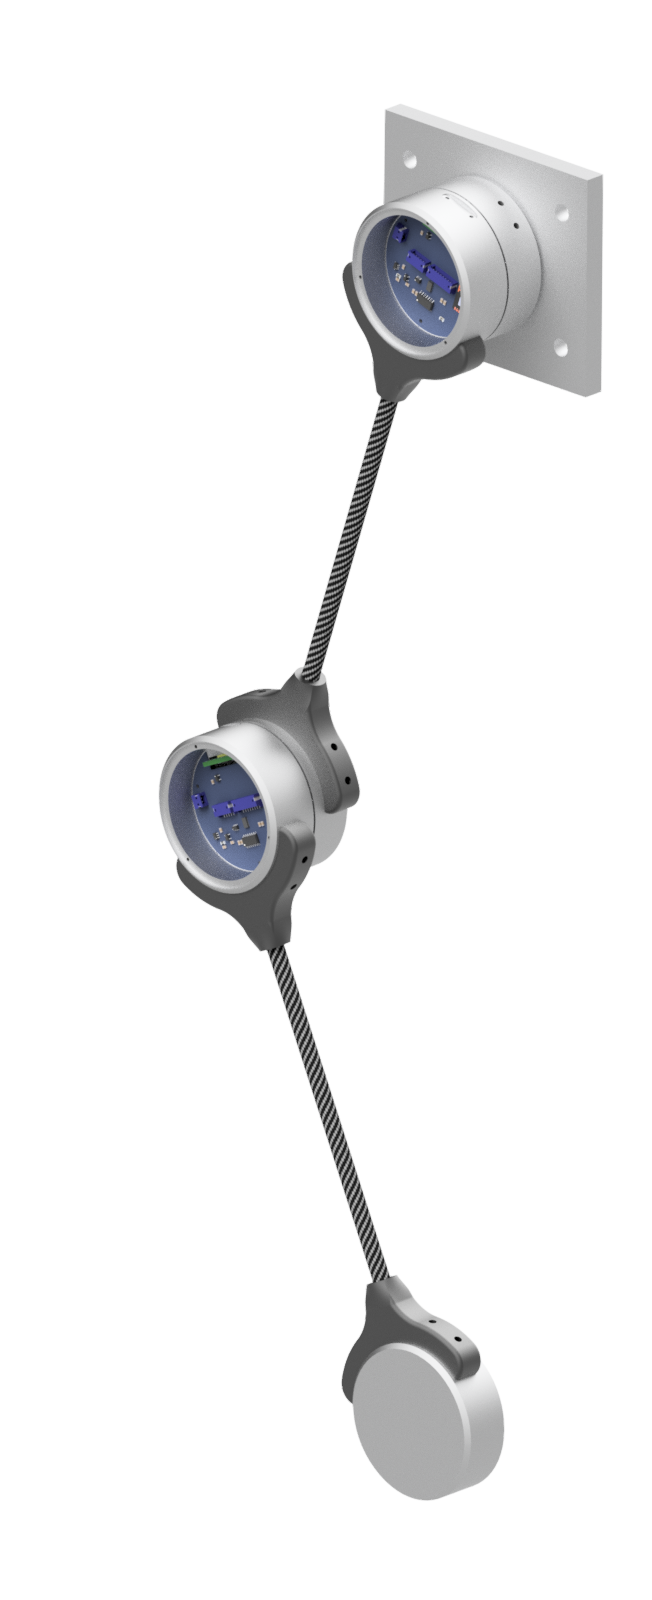
\includegraphics[width=.32\linewidth]{graphics/pendulum_assembly}
	\end{figure}
\end{frame}
\note{Thomas}

\section{Implementation}

\begin{frame}[c]\frametitle{Implementation of Joint Board PCB}
\begin{figure}
	\centering
	\begin{subfigure}{.5\textwidth}
	  \centering
	  \includegraphics[width=.9\linewidth]{graphics/joint_board_pic}
	\end{subfigure}%
	\begin{subfigure}{.5\textwidth}
	  \centering
	  \includegraphics[width=.9\linewidth]{graphics/joint_board_pop_pic}
	\end{subfigure}
	\end{figure}
\end{frame}
\note{The PCB design was sent to China and the PCB shown in the left picture was delivered.
The components was soldered on the PCB using soldering paste, a pick and place machine and a reflow oven.
The result is shown on the right picture.
As it can be seen several fixes was needed to achieve the full functionality.
There are room for improvements and a version 2 of the PCB.
}

\begin{frame}[c]\frametitle{Implementation of Full System}
	\begin{figure}
		\centering
		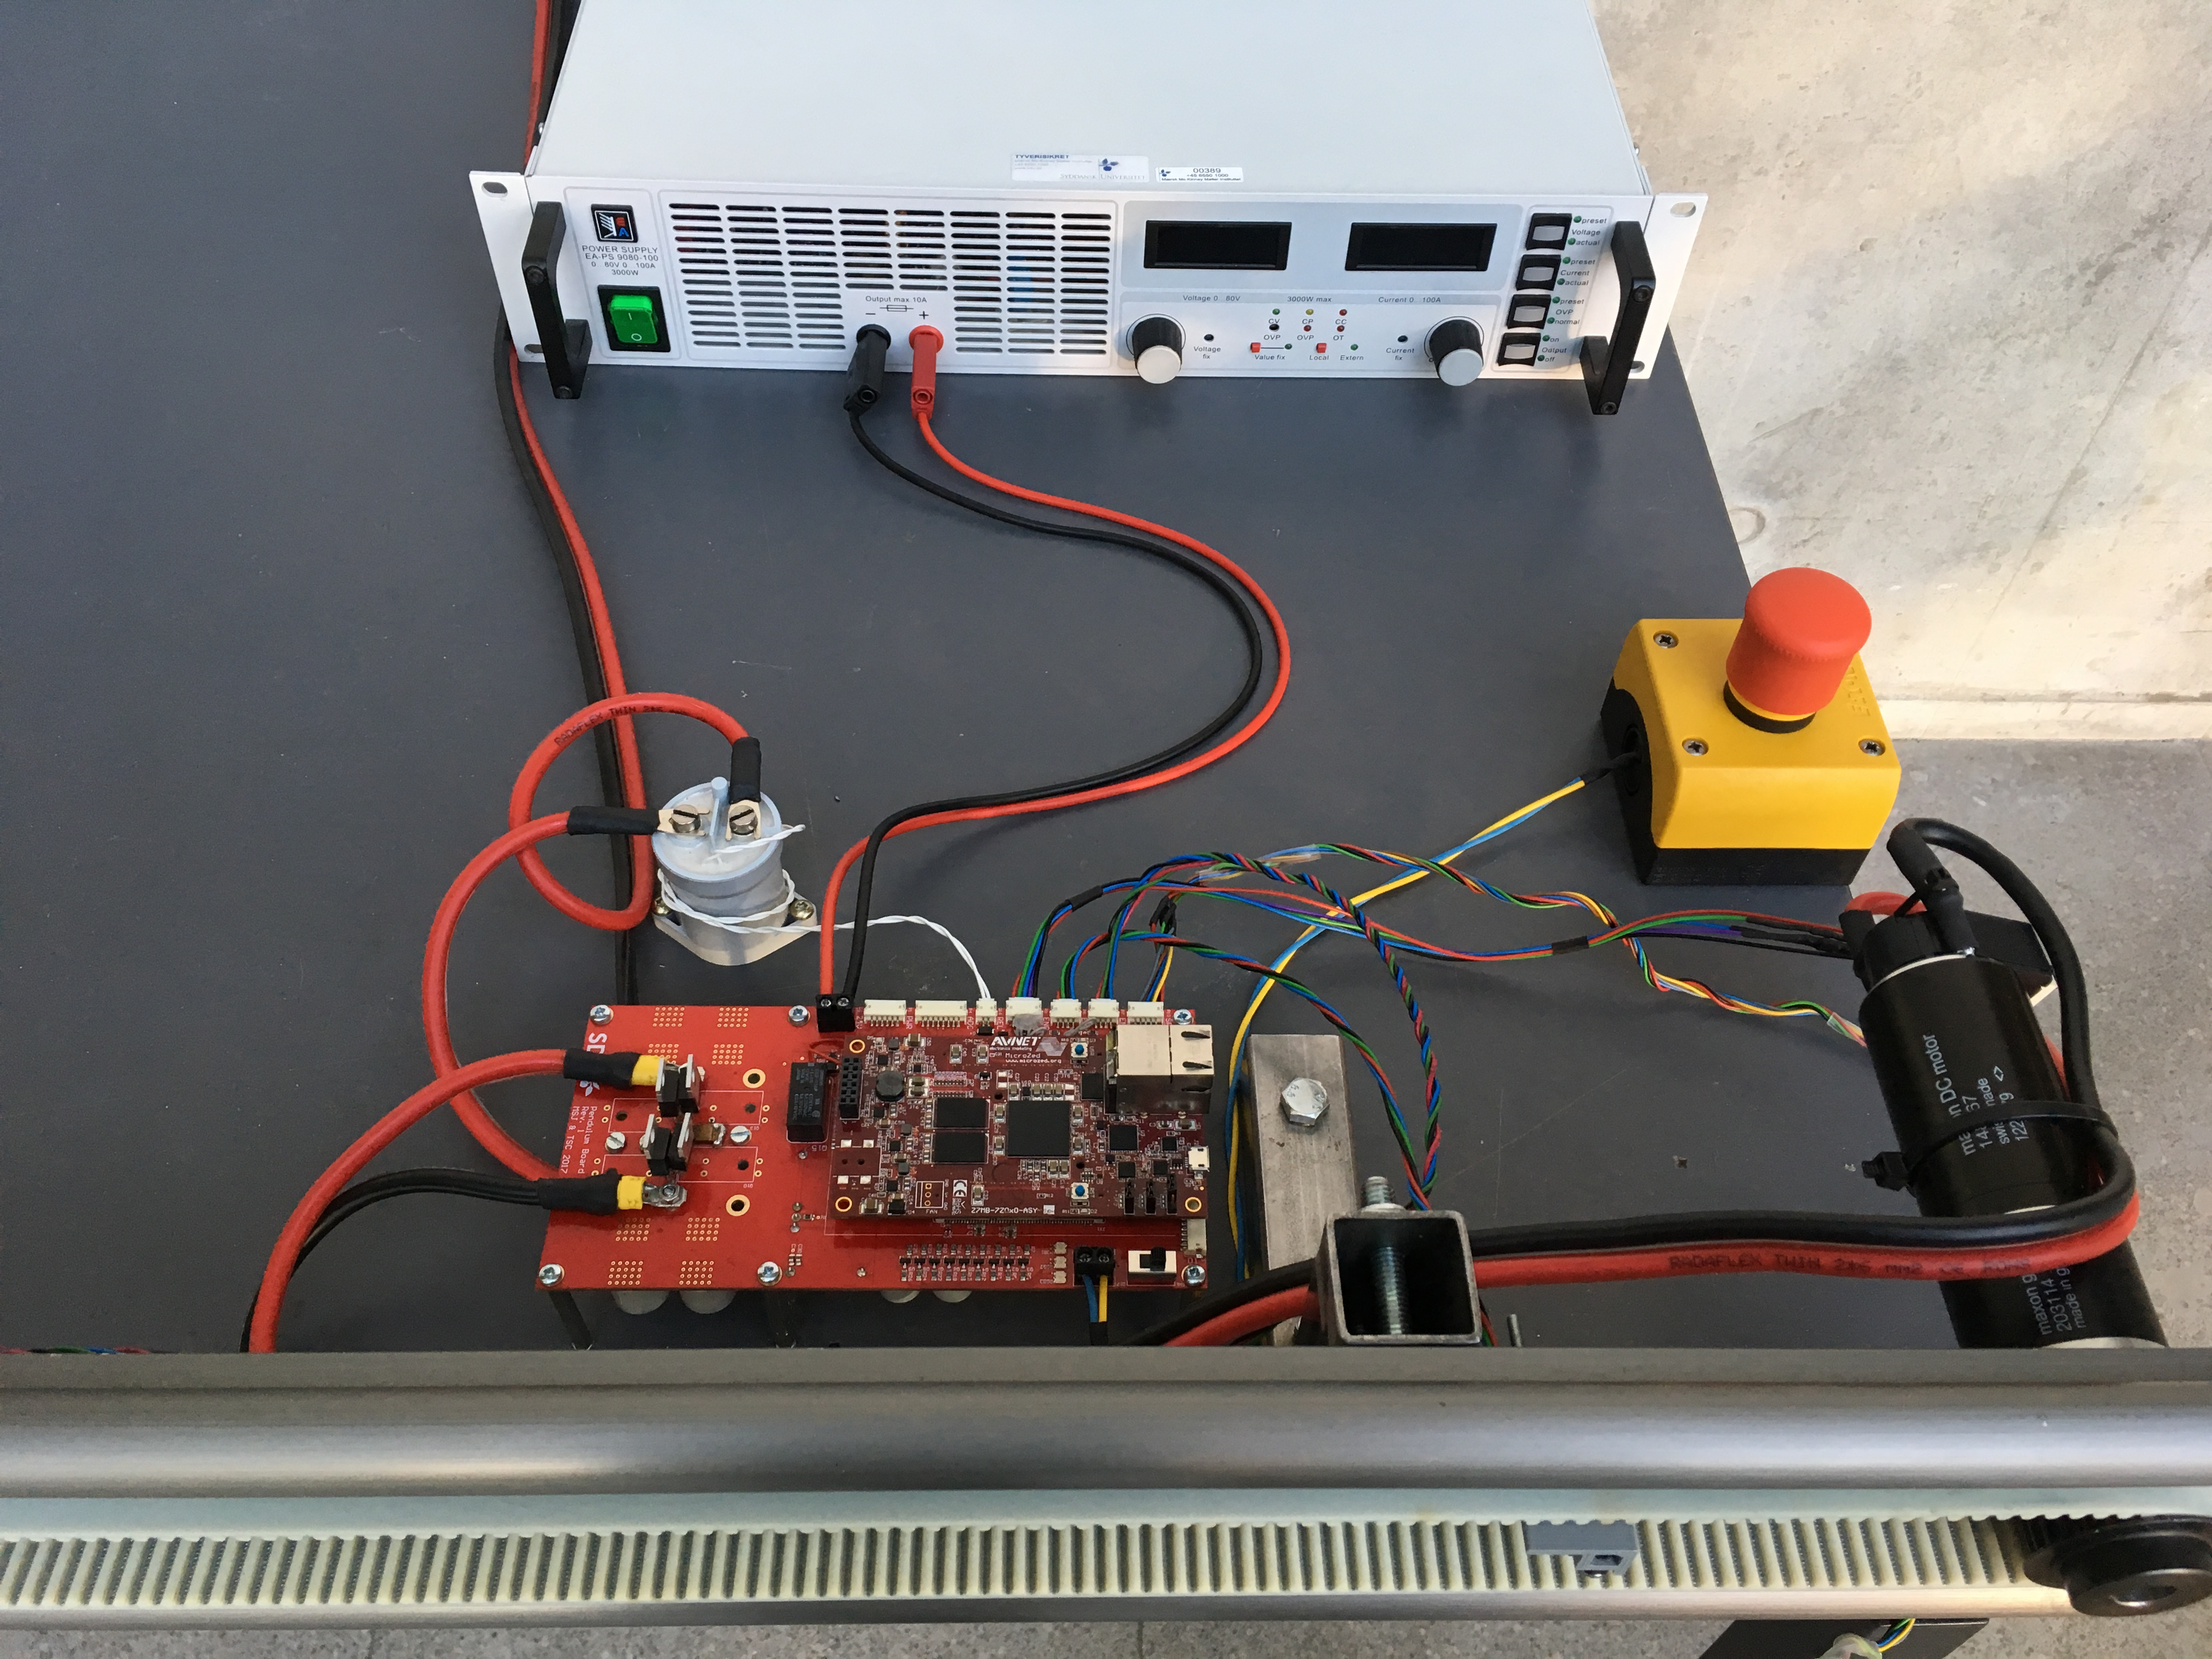
\includegraphics[width=.9\linewidth]{graphics/full_system_finish_high}
	\end{figure}
\end{frame}
\note{Mikkel}

\begin{frame}[c]\frametitle{Implementation Pendulum Assembly}
	\begin{figure}
		\centering
		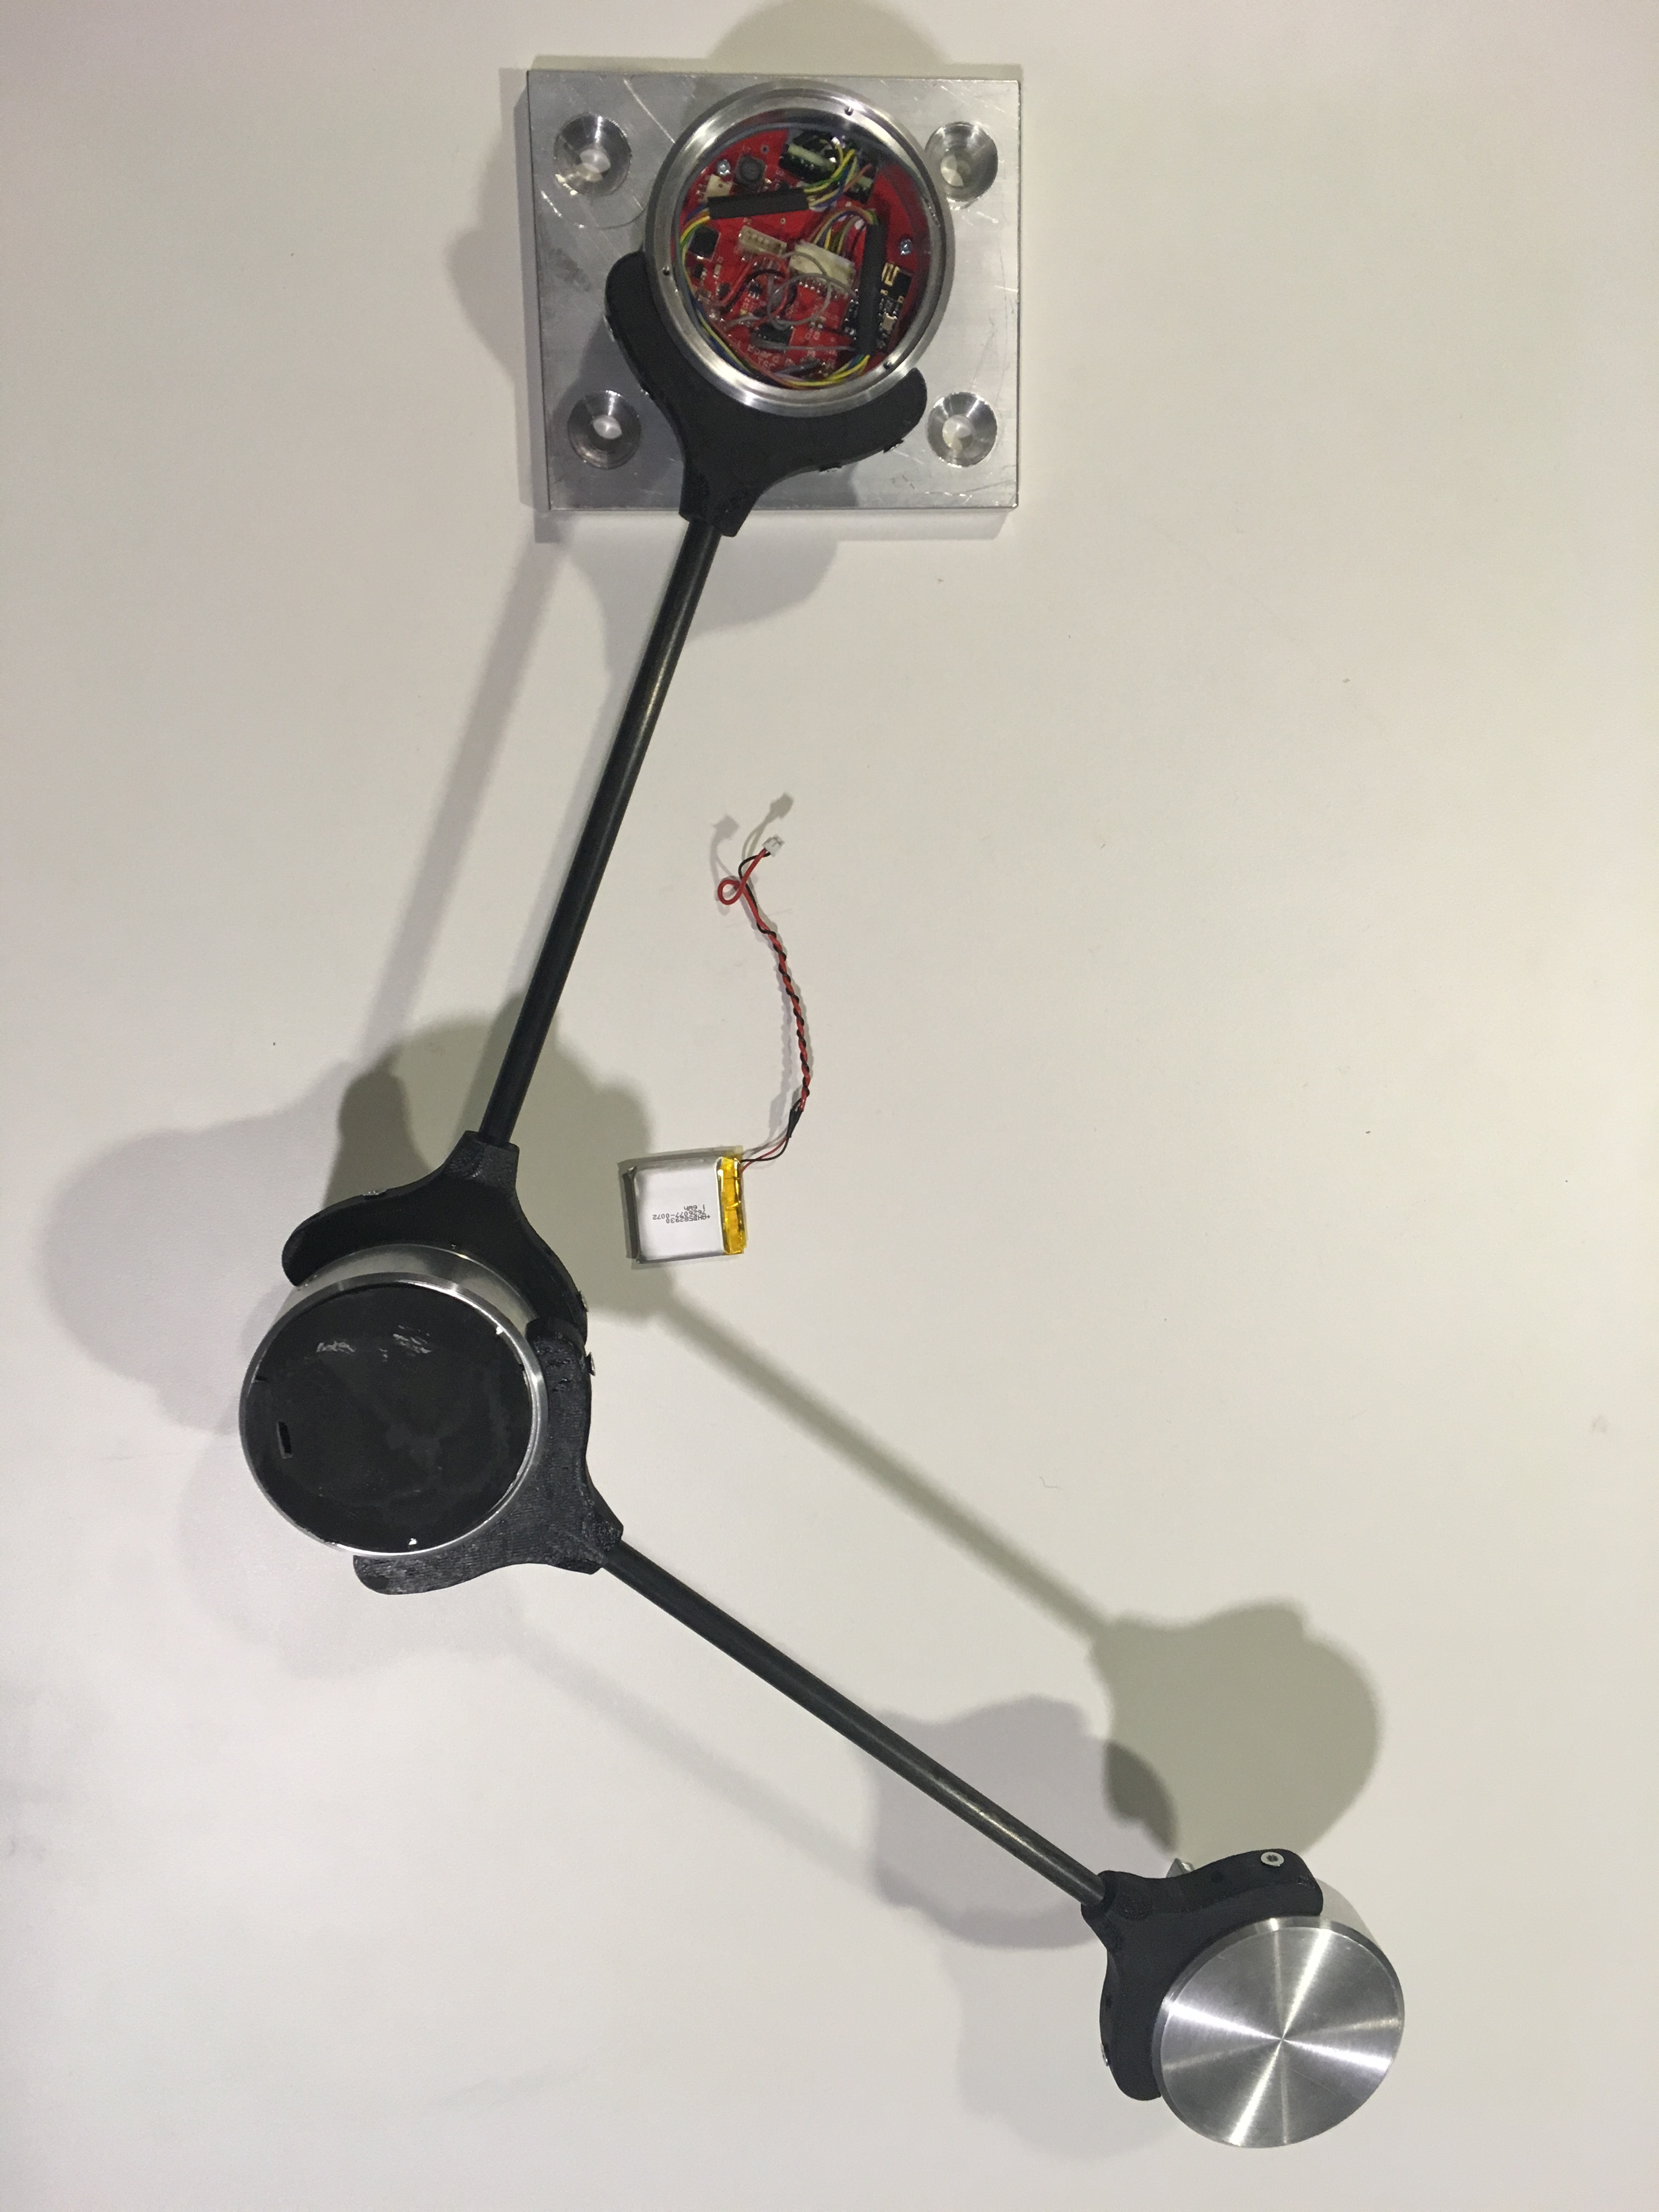
\includegraphics[width=.4\linewidth]{graphics/joint_ass_real}
	\end{figure}
\end{frame}
\note{Mikkel}

\section{Verification}

\begin{frame}[c]\frametitle{Verification of Requirement}
	\begin{enumerate}
		\item[4.] \alert{Position of the cart and joint angles should be measured.}
	\end{enumerate}
\end{frame}
\note{Thomas}

\begin{frame}[c]\frametitle{Test of Single Pendulum}
    \begin{figure}[h]
		\centering
		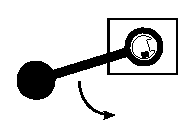
\includegraphics[width=.5\linewidth]{graphics/single_pendulum}
	\end{figure}
\end{frame}
\note{Thomas}

\begin{frame}[c]\frametitle{Test of Single Pendulum}
    \begin{figure}[h]
		\centering
		% This file was created by matlab2tikz.
%
%The latest updates can be retrieved from
%  http://www.mathworks.com/matlabcentral/fileexchange/22022-matlab2tikz-matlab2tikz
%where you can also make suggestions and rate matlab2tikz.
%
\definecolor{mycolor1}{rgb}{0.00000,0.44700,0.74100}%
%
\begin{tikzpicture}

\begin{axis}[%
width=.8\textwidth,
height=2in,
at={(0.758in,0.481in)},
scale only axis,
xmin=60000,
xmax=100000,
xlabel style={font=\color{white!15!black}},
xlabel={Time [ms]},
ymin=4000,
ymax=5200,
ylabel style={font=\color{white!15!black}},
ylabel={Angle [ticks]},
axis background/.style={fill=white},
title style={font=\bfseries},
title={Joint Angle},
axis x line*=bottom,
axis y line*=left
]
\addplot[only marks, mark=*, mark options={}, mark size=0.5000pt, draw=mycolor1] table[row sep=crcr]{%
x	y\\
58576	4739\\
58577	4742\\
58578	4746\\
58579	4750\\
58580	4753\\
58581	4757\\
58582	4761\\
58583	4764\\
58584	4768\\
58585	4771\\
58586	4775\\
58587	4779\\
58589	4786\\
58590	4789\\
58591	4793\\
58595	4807\\
58596	4810\\
58597	4814\\
58599	4821\\
58600	4824\\
58601	4828\\
58603	4835\\
58604	4838\\
58605	4841\\
58607	4848\\
58609	4855\\
58611	4861\\
58612	4864\\
58614	4871\\
58615	4874\\
58616	4877\\
58618	4883\\
58619	4886\\
58622	4896\\
58625	4905\\
58626	4908\\
58627	4911\\
58629	4917\\
58630	4920\\
58632	4926\\
58633	4929\\
58634	4932\\
58635	4934\\
58636	4937\\
58637	4940\\
58638	4943\\
58640	4948\\
58641	4951\\
58642	4954\\
58644	4959\\
58645	4962\\
58646	4964\\
58647	4967\\
58650	4975\\
58652	4980\\
58654	4985\\
58655	4987\\
58656	4989\\
58657	4992\\
58658	4994\\
58659	4996\\
58660	4999\\
58661	5001\\
58663	5006\\
58665	5010\\
58666	5012\\
58667	5015\\
58668	5017\\
58671	5023\\
58672	5025\\
58673	5027\\
58674	5029\\
58676	5033\\
58677	5035\\
58678	5037\\
58680	5041\\
58682	5044\\
58683	5046\\
58684	5048\\
58686	5052\\
58687	5053\\
58688	5055\\
58689	5057\\
58690	5058\\
58691	5060\\
58693	5063\\
58694	5064\\
58695	5066\\
58696	5067\\
58697	5069\\
58698	5070\\
58699	5071\\
58700	5073\\
58701	5074\\
58702	5075\\
58703	5077\\
58704	5078\\
58705	5079\\
58706	5080\\
58707	5082\\
58708	5083\\
58710	5085\\
58711	5086\\
58712	5087\\
58715	5090\\
58716	5091\\
58717	5092\\
58718	5093\\
58720	5095\\
58721	5095\\
58722	5096\\
58725	5099\\
58726	5099\\
58727	5100\\
58728	5101\\
58730	5102\\
58737	5105\\
58738	5106\\
58740	5106\\
58741	5107\\
58743	5107\\
58744	5108\\
58745	5108\\
58751	5108\\
58752	5109\\
58754	5109\\
58757	5108\\
58758	5108\\
58759	5108\\
58760	5108\\
58761	5108\\
58762	5107\\
58763	5107\\
58764	5107\\
58766	5106\\
58767	5106\\
58769	5105\\
58770	5105\\
58772	5104\\
58773	5103\\
58774	5103\\
58776	5101\\
58777	5101\\
58778	5100\\
58779	5100\\
58780	5099\\
58782	5097\\
58785	5095\\
58786	5094\\
58787	5093\\
58788	5092\\
58790	5090\\
58791	5089\\
58792	5088\\
58793	5087\\
58794	5086\\
58795	5085\\
58799	5081\\
58800	5080\\
58801	5078\\
58802	5077\\
58804	5075\\
58805	5073\\
58807	5071\\
58808	5069\\
58809	5068\\
58810	5066\\
58812	5063\\
58813	5062\\
58814	5060\\
58815	5059\\
58816	5057\\
58817	5056\\
58818	5054\\
58819	5052\\
58820	5050\\
58821	5049\\
58822	5047\\
58823	5045\\
58824	5043\\
58825	5041\\
58828	5036\\
58829	5034\\
58831	5030\\
58832	5028\\
58833	5026\\
58834	5024\\
58835	5022\\
58836	5020\\
58837	5018\\
58839	5013\\
58840	5011\\
58842	5007\\
58843	5005\\
58844	5002\\
58848	4993\\
58849	4990\\
58850	4988\\
58852	4983\\
58853	4981\\
58854	4978\\
58855	4976\\
58856	4973\\
58857	4971\\
58859	4966\\
58860	4963\\
58861	4961\\
58863	4955\\
58864	4953\\
58865	4950\\
58867	4944\\
58871	4933\\
58872	4930\\
58873	4927\\
58874	4924\\
58875	4922\\
58876	4919\\
58877	4916\\
58878	4913\\
58879	4910\\
58880	4907\\
58881	4904\\
58882	4901\\
58883	4898\\
58884	4895\\
58885	4891\\
58887	4885\\
58888	4882\\
58889	4879\\
58890	4876\\
58891	4873\\
58892	4870\\
58893	4866\\
58894	4863\\
58895	4860\\
58896	4857\\
58897	4854\\
58899	4847\\
58902	4837\\
58903	4834\\
58904	4830\\
58905	4827\\
58906	4823\\
58907	4820\\
58908	4816\\
58909	4813\\
58911	4806\\
58912	4803\\
58913	4799\\
58914	4795\\
58915	4792\\
58916	4788\\
58917	4785\\
58918	4781\\
58920	4774\\
58921	4771\\
58923	4764\\
58924	4760\\
58926	4753\\
58927	4749\\
58929	4742\\
58930	4738\\
58931	4735\\
58932	4731\\
58934	4723\\
58937	4712\\
58938	4709\\
58939	4705\\
58940	4701\\
58941	4697\\
58942	4694\\
58943	4690\\
58945	4682\\
58946	4679\\
58947	4675\\
58949	4668\\
58950	4664\\
58951	4660\\
58954	4649\\
58956	4641\\
58957	4637\\
58958	4634\\
58959	4630\\
58961	4622\\
58962	4618\\
58963	4615\\
58965	4607\\
58966	4603\\
58969	4592\\
58970	4588\\
58971	4584\\
58973	4577\\
58974	4573\\
58977	4562\\
58978	4558\\
58980	4550\\
58981	4547\\
58982	4543\\
58983	4539\\
58987	4524\\
58988	4520\\
58989	4516\\
58990	4513\\
58991	4509\\
58992	4505\\
58993	4501\\
58994	4498\\
58997	4487\\
58998	4483\\
58999	4479\\
59001	4472\\
59002	4468\\
59004	4461\\
59005	4458\\
59006	4454\\
59007	4450\\
59008	4447\\
59009	4443\\
59010	4439\\
59011	4436\\
59012	4432\\
59013	4429\\
59014	4425\\
59015	4422\\
59016	4418\\
59017	4414\\
59018	4411\\
59019	4408\\
59020	4404\\
59021	4401\\
59022	4397\\
59023	4394\\
59025	4387\\
59027	4380\\
59028	4377\\
59029	4374\\
59031	4367\\
59032	4364\\
59034	4357\\
59035	4354\\
59036	4351\\
59037	4347\\
59038	4344\\
59039	4341\\
59040	4338\\
59042	4332\\
59043	4328\\
59044	4325\\
59045	4322\\
59046	4319\\
59047	4316\\
59048	4313\\
59049	4310\\
59050	4307\\
59051	4304\\
59053	4298\\
59054	4295\\
59055	4292\\
59059	4281\\
59061	4275\\
59065	4264\\
59067	4259\\
59068	4256\\
59069	4253\\
59070	4251\\
59072	4246\\
59075	4238\\
59076	4235\\
59078	4230\\
59079	4228\\
59083	4218\\
59084	4216\\
59086	4211\\
59088	4207\\
59090	4203\\
59091	4200\\
59093	4196\\
59094	4194\\
59096	4190\\
59097	4188\\
59098	4186\\
59099	4184\\
59100	4182\\
59101	4180\\
59102	4178\\
59103	4176\\
59104	4174\\
59105	4173\\
59107	4169\\
59108	4167\\
59110	4164\\
59111	4162\\
59113	4159\\
59114	4157\\
59115	4156\\
59116	4154\\
59117	4153\\
59118	4151\\
59119	4150\\
59121	4147\\
59122	4145\\
59123	4144\\
59124	4142\\
59125	4141\\
59126	4140\\
59127	4138\\
59128	4137\\
59129	4136\\
59130	4135\\
59132	4132\\
59133	4131\\
59135	4129\\
59136	4128\\
59137	4127\\
59139	4125\\
59140	4124\\
59141	4123\\
59142	4122\\
59144	4120\\
59145	4119\\
59147	4118\\
59148	4117\\
59151	4115\\
59152	4114\\
59153	4114\\
59154	4113\\
59155	4112\\
59156	4112\\
59158	4111\\
59159	4110\\
59160	4110\\
59161	4110\\
59162	4109\\
59164	4108\\
59165	4108\\
59167	4108\\
59168	4107\\
59169	4107\\
59170	4107\\
59171	4107\\
59173	4106\\
59174	4106\\
59175	4106\\
59176	4106\\
59177	4106\\
59178	4106\\
59180	4106\\
59181	4106\\
59182	4106\\
59184	4107\\
59185	4107\\
59186	4107\\
59187	4107\\
59188	4108\\
59190	4108\\
59192	4109\\
59193	4109\\
59195	4110\\
59197	4111\\
59198	4112\\
59199	4112\\
59201	4113\\
59202	4114\\
59203	4114\\
59205	4116\\
59208	4118\\
59210	4120\\
59215	4124\\
59216	4125\\
59217	4126\\
59218	4127\\
59219	4128\\
59220	4129\\
59222	4132\\
59223	4133\\
59225	4135\\
59226	4136\\
59228	4139\\
59229	4140\\
59230	4141\\
59232	4144\\
59233	4145\\
59235	4148\\
59237	4151\\
59238	4153\\
59239	4154\\
59240	4156\\
59242	4159\\
59243	4161\\
59244	4162\\
59245	4164\\
59246	4166\\
59247	4167\\
59248	4169\\
59249	4171\\
59251	4174\\
59252	4176\\
59254	4180\\
59255	4182\\
59256	4184\\
59258	4188\\
59259	4190\\
59262	4196\\
59263	4198\\
59264	4200\\
59265	4202\\
59267	4207\\
59268	4209\\
59269	4211\\
59270	4213\\
59272	4218\\
59273	4220\\
59275	4225\\
59276	4227\\
59277	4230\\
59278	4232\\
59279	4235\\
59280	4237\\
59283	4245\\
59284	4247\\
59285	4250\\
59286	4253\\
59287	4255\\
59288	4258\\
59289	4260\\
59291	4266\\
59292	4268\\
59293	4271\\
59295	4277\\
59296	4279\\
59298	4285\\
59299	4288\\
59301	4293\\
59302	4296\\
59304	4302\\
59305	4305\\
59306	4308\\
59307	4311\\
59308	4314\\
59309	4317\\
59310	4320\\
59311	4323\\
59313	4330\\
59314	4333\\
59315	4336\\
59317	4342\\
59318	4345\\
59319	4348\\
59320	4352\\
59321	4355\\
59323	4361\\
59324	4365\\
59325	4368\\
59327	4374\\
59328	4378\\
59330	4384\\
59331	4387\\
59332	4391\\
59334	4398\\
59335	4401\\
59337	4408\\
59339	4415\\
59340	4418\\
59341	4422\\
59342	4425\\
59343	4429\\
59344	4432\\
59345	4436\\
59346	4439\\
59347	4443\\
59348	4447\\
59349	4450\\
59350	4454\\
59351	4457\\
59353	4464\\
59355	4471\\
59356	4475\\
59357	4479\\
59358	4482\\
59360	4489\\
59362	4497\\
59363	4500\\
59364	4504\\
59365	4508\\
59366	4511\\
59368	4519\\
59369	4523\\
59370	4526\\
59371	4530\\
59372	4534\\
59373	4537\\
59374	4541\\
59376	4549\\
59377	4552\\
59378	4556\\
59379	4560\\
59380	4563\\
59381	4567\\
59382	4571\\
59383	4574\\
59385	4582\\
59386	4585\\
59387	4589\\
59388	4593\\
59389	4597\\
59391	4604\\
59392	4608\\
59394	4615\\
59395	4619\\
59396	4623\\
59397	4627\\
59398	4630\\
59399	4634\\
59400	4638\\
59401	4642\\
59402	4645\\
59403	4649\\
59404	4653\\
59405	4656\\
59406	4660\\
59407	4664\\
59408	4667\\
59409	4671\\
59410	4675\\
59411	4678\\
59412	4682\\
59413	4686\\
59414	4689\\
59416	4697\\
59417	4700\\
59418	4704\\
59419	4708\\
59424	4726\\
59426	4733\\
59427	4737\\
59428	4740\\
59429	4744\\
59430	4747\\
59431	4751\\
59432	4755\\
59433	4758\\
59434	4762\\
59437	4772\\
59439	4779\\
59440	4782\\
59441	4786\\
59442	4789\\
59443	4792\\
59444	4796\\
59445	4799\\
59446	4803\\
59447	4806\\
59448	4810\\
59449	4813\\
59450	4816\\
59452	4823\\
59453	4826\\
59454	4830\\
59455	4833\\
59456	4836\\
59457	4839\\
59458	4843\\
59459	4846\\
59462	4856\\
59464	4862\\
59465	4865\\
59467	4871\\
59468	4874\\
59469	4877\\
59470	4880\\
59473	4889\\
59474	4892\\
59475	4895\\
59477	4901\\
59478	4904\\
59479	4907\\
59481	4912\\
59482	4915\\
59483	4918\\
59485	4924\\
59486	4927\\
59487	4929\\
59489	4935\\
59490	4937\\
59492	4943\\
59493	4945\\
59495	4951\\
59496	4953\\
59499	4961\\
59500	4963\\
59501	4966\\
59502	4968\\
59503	4971\\
59505	4975\\
59506	4978\\
59507	4980\\
59509	4984\\
59510	4987\\
59511	4989\\
59512	4991\\
59513	4993\\
59514	4996\\
59516	5000\\
59517	5002\\
59520	5008\\
59521	5010\\
59523	5014\\
59525	5018\\
59526	5020\\
59527	5022\\
59528	5024\\
59532	5031\\
59533	5033\\
59535	5037\\
59536	5038\\
59537	5040\\
59538	5042\\
59539	5043\\
59541	5046\\
59542	5048\\
59543	5050\\
59545	5053\\
59546	5054\\
59548	5057\\
59549	5058\\
59550	5060\\
59551	5061\\
59553	5063\\
59554	5065\\
59556	5067\\
59558	5069\\
59559	5070\\
59560	5071\\
59562	5074\\
59563	5075\\
59564	5076\\
59566	5077\\
59567	5078\\
59569	5080\\
59571	5082\\
59572	5083\\
59574	5084\\
59575	5085\\
59577	5086\\
59579	5087\\
59580	5088\\
59581	5089\\
59583	5090\\
59584	5090\\
59585	5091\\
59586	5091\\
59587	5091\\
59588	5092\\
59589	5092\\
59590	5093\\
59591	5093\\
59592	5093\\
59593	5093\\
59595	5094\\
59596	5094\\
59597	5094\\
59599	5095\\
59600	5095\\
59602	5095\\
59603	5095\\
59604	5095\\
59605	5095\\
59606	5095\\
59608	5095\\
59609	5094\\
59610	5094\\
59611	5094\\
59612	5094\\
59613	5094\\
59614	5093\\
59615	5093\\
59616	5093\\
59617	5092\\
59618	5092\\
59619	5092\\
59620	5091\\
59622	5090\\
59623	5090\\
59626	5088\\
59628	5087\\
59629	5087\\
59630	5086\\
59632	5085\\
59633	5084\\
59634	5083\\
59635	5082\\
59636	5082\\
59637	5081\\
59638	5080\\
59639	5079\\
59642	5076\\
59643	5075\\
59645	5073\\
59646	5072\\
59647	5071\\
59648	5070\\
59649	5069\\
59650	5068\\
59651	5067\\
59653	5064\\
59655	5062\\
59656	5060\\
59657	5059\\
59659	5056\\
59660	5055\\
59662	5052\\
59663	5051\\
59664	5049\\
59665	5048\\
59666	5046\\
59667	5044\\
59668	5043\\
59670	5040\\
59671	5038\\
59672	5036\\
59673	5034\\
59674	5033\\
59675	5031\\
59677	5027\\
59678	5026\\
59680	5022\\
59681	5020\\
59682	5018\\
59684	5014\\
59685	5012\\
59687	5008\\
59688	5006\\
59689	5004\\
59690	5002\\
59691	5000\\
59692	4997\\
59693	4995\\
59694	4993\\
59696	4989\\
59697	4986\\
59698	4984\\
59700	4980\\
59701	4977\\
59703	4973\\
59706	4965\\
59707	4963\\
59708	4960\\
59709	4958\\
59711	4953\\
59714	4945\\
59715	4942\\
59717	4937\\
59718	4934\\
59720	4929\\
59721	4926\\
59722	4923\\
59724	4918\\
59725	4915\\
59727	4909\\
59728	4907\\
59731	4898\\
59732	4895\\
59733	4892\\
59734	4889\\
59736	4883\\
59738	4877\\
59739	4874\\
59740	4871\\
59742	4865\\
59743	4862\\
59744	4859\\
59746	4852\\
59747	4849\\
59749	4843\\
59750	4840\\
59751	4836\\
59756	4820\\
59757	4817\\
59758	4813\\
59760	4807\\
59761	4803\\
59762	4800\\
59763	4796\\
59766	4786\\
59768	4779\\
59769	4776\\
59771	4769\\
59772	4766\\
59773	4762\\
59775	4755\\
59776	4752\\
59777	4748\\
59779	4741\\
59780	4737\\
59781	4734\\
59782	4730\\
59783	4727\\
59784	4723\\
59785	4720\\
59787	4712\\
59788	4709\\
59789	4705\\
59791	4698\\
59792	4694\\
59793	4690\\
59794	4687\\
59797	4676\\
59798	4672\\
59800	4665\\
59801	4662\\
59802	4658\\
59803	4654\\
59805	4647\\
59806	4643\\
59807	4639\\
59808	4636\\
59812	4621\\
59813	4617\\
59814	4614\\
59815	4610\\
59816	4606\\
59817	4603\\
59818	4599\\
59820	4591\\
59821	4588\\
59822	4584\\
59823	4580\\
59825	4573\\
59826	4570\\
59828	4562\\
59829	4559\\
59830	4555\\
59832	4548\\
59833	4544\\
59834	4540\\
59836	4533\\
59837	4529\\
59838	4526\\
59839	4522\\
59841	4515\\
59842	4511\\
59844	4504\\
59845	4500\\
59846	4496\\
59847	4493\\
59849	4486\\
59850	4482\\
59851	4479\\
59853	4472\\
59854	4468\\
59855	4464\\
59856	4461\\
59858	4454\\
59859	4451\\
59861	4444\\
59864	4433\\
59865	4430\\
59866	4426\\
59868	4419\\
59870	4412\\
59871	4409\\
59872	4406\\
59873	4402\\
59874	4399\\
59876	4392\\
59879	4383\\
59880	4379\\
59882	4373\\
59884	4367\\
59885	4363\\
59886	4360\\
59887	4357\\
59888	4354\\
59890	4348\\
59891	4345\\
59892	4342\\
59894	4335\\
59895	4332\\
59896	4329\\
59898	4323\\
59899	4320\\
59900	4317\\
59902	4312\\
59903	4309\\
59904	4306\\
59905	4303\\
59906	4300\\
59907	4297\\
59908	4295\\
59909	4292\\
59911	4286\\
59912	4284\\
59913	4281\\
59914	4278\\
59915	4276\\
59916	4273\\
59917	4270\\
59918	4268\\
59919	4265\\
59920	4263\\
59921	4260\\
59923	4255\\
59924	4253\\
59925	4250\\
59926	4248\\
59927	4245\\
59930	4238\\
59931	4236\\
59933	4231\\
59934	4229\\
59935	4226\\
59937	4222\\
59938	4220\\
59939	4217\\
59941	4213\\
59942	4211\\
59944	4207\\
59945	4205\\
59946	4203\\
59947	4201\\
59948	4199\\
59949	4197\\
59950	4195\\
59951	4193\\
59952	4191\\
59954	4187\\
59955	4186\\
59956	4184\\
59957	4182\\
59959	4179\\
59960	4177\\
59961	4175\\
59962	4174\\
59963	4172\\
59964	4171\\
59965	4169\\
59966	4168\\
59967	4166\\
59968	4165\\
59969	4163\\
59971	4160\\
59972	4159\\
59974	4156\\
59975	4155\\
59976	4154\\
59977	4152\\
59978	4151\\
59979	4150\\
59981	4147\\
59983	4145\\
59984	4144\\
59985	4143\\
59987	4141\\
59988	4140\\
59989	4139\\
59991	4137\\
59993	4135\\
59996	4133\\
59997	4132\\
59998	4131\\
59999	4130\\
60000	4130\\
60001	4129\\
60002	4128\\
60003	4128\\
60006	4126\\
60007	4125\\
60009	4124\\
60010	4124\\
60012	4123\\
60013	4123\\
60015	4122\\
60017	4121\\
60018	4121\\
60020	4121\\
60021	4120\\
60022	4120\\
60023	4120\\
60024	4120\\
60025	4120\\
60026	4120\\
60027	4120\\
60028	4120\\
60029	4120\\
60033	4120\\
60035	4120\\
60036	4120\\
60039	4121\\
60043	4122\\
60046	4124\\
60048	4125\\
60049	4125\\
60050	4126\\
60052	4127\\
60054	4128\\
60055	4129\\
60056	4129\\
60057	4130\\
60058	4131\\
60059	4132\\
60060	4132\\
60061	4133\\
60062	4134\\
60063	4135\\
60064	4136\\
60067	4138\\
60069	4140\\
60071	4142\\
60072	4143\\
60075	4147\\
60076	4148\\
60077	4149\\
60078	4150\\
60079	4152\\
60080	4153\\
60081	4154\\
60082	4156\\
60083	4157\\
60086	4161\\
60087	4162\\
60088	4164\\
60089	4165\\
60090	4167\\
60094	4173\\
60095	4174\\
60097	4178\\
60098	4179\\
60099	4181\\
60101	4185\\
60102	4186\\
60103	4188\\
60104	4190\\
60105	4192\\
60106	4194\\
60107	4195\\
60109	4199\\
60110	4201\\
60111	4203\\
60112	4205\\
60113	4207\\
60115	4212\\
60116	4214\\
60117	4216\\
60119	4220\\
60120	4222\\
60121	4224\\
60122	4227\\
60123	4229\\
60124	4231\\
60126	4236\\
60127	4238\\
60128	4240\\
60129	4243\\
60130	4245\\
60131	4248\\
60132	4250\\
60134	4255\\
60135	4258\\
60136	4260\\
60137	4263\\
60138	4265\\
60139	4268\\
60140	4270\\
60141	4273\\
60142	4275\\
60143	4278\\
60144	4281\\
60148	4291\\
60149	4294\\
60150	4297\\
60151	4300\\
60152	4303\\
60153	4305\\
60154	4308\\
60155	4311\\
60156	4314\\
60158	4320\\
60160	4326\\
60163	4335\\
60164	4338\\
60165	4341\\
60166	4344\\
60167	4347\\
60169	4353\\
60170	4356\\
60172	4362\\
60173	4365\\
60174	4368\\
60176	4375\\
60177	4378\\
60178	4381\\
60180	4387\\
60181	4391\\
60182	4394\\
60183	4397\\
60184	4400\\
60186	4407\\
60188	4414\\
60189	4417\\
60191	4424\\
60192	4427\\
60193	4431\\
60196	4441\\
60197	4444\\
60198	4448\\
60199	4451\\
60200	4455\\
60203	4465\\
60204	4468\\
60206	4475\\
60207	4479\\
60208	4482\\
60209	4486\\
60210	4489\\
60212	4497\\
60214	4504\\
60216	4511\\
60218	4518\\
60219	4522\\
60220	4525\\
60222	4532\\
60223	4536\\
60224	4540\\
60226	4547\\
60227	4551\\
60228	4554\\
60230	4561\\
60231	4565\\
60233	4572\\
60234	4576\\
60235	4579\\
60236	4583\\
60237	4586\\
60239	4594\\
60241	4601\\
60243	4608\\
60249	4630\\
60250	4634\\
60252	4641\\
60253	4644\\
60254	4648\\
60255	4652\\
60256	4655\\
60258	4662\\
60261	4673\\
60262	4677\\
60264	4684\\
60265	4687\\
60266	4691\\
60267	4694\\
60268	4698\\
60269	4701\\
60270	4705\\
60271	4709\\
60273	4716\\
60274	4719\\
60277	4730\\
60278	4733\\
60280	4740\\
60281	4744\\
60282	4747\\
60283	4751\\
60284	4754\\
60285	4757\\
60286	4761\\
60287	4764\\
60288	4768\\
60290	4774\\
60291	4778\\
60292	4781\\
60293	4784\\
60294	4787\\
60296	4794\\
60299	4804\\
60301	4811\\
60302	4814\\
60303	4817\\
60304	4820\\
60305	4823\\
60306	4827\\
60307	4830\\
60308	4833\\
60309	4836\\
60310	4839\\
60311	4842\\
60312	4846\\
60313	4849\\
60314	4852\\
60315	4855\\
60316	4858\\
60317	4861\\
60320	4870\\
60323	4879\\
60325	4884\\
60326	4887\\
60328	4893\\
60329	4896\\
60330	4898\\
60331	4901\\
60333	4907\\
60336	4915\\
60338	4920\\
60340	4926\\
60341	4928\\
60343	4934\\
60344	4936\\
60345	4939\\
60346	4941\\
60347	4944\\
60348	4946\\
60349	4949\\
60350	4951\\
60352	4956\\
60353	4958\\
60356	4965\\
60358	4970\\
60359	4972\\
60360	4974\\
60362	4979\\
60363	4981\\
60364	4983\\
60365	4985\\
60366	4987\\
60368	4991\\
60369	4993\\
60370	4995\\
60371	4997\\
60372	4999\\
60373	5001\\
60374	5003\\
60375	5005\\
60376	5007\\
60377	5009\\
60378	5011\\
60380	5014\\
60381	5016\\
60382	5018\\
60384	5021\\
60385	5023\\
60386	5025\\
60387	5026\\
60388	5028\\
60389	5030\\
60391	5033\\
60392	5034\\
60393	5036\\
60394	5037\\
60395	5039\\
60396	5040\\
60398	5043\\
60399	5044\\
60401	5047\\
60402	5048\\
60403	5050\\
60404	5051\\
60405	5052\\
60406	5053\\
60407	5054\\
60408	5056\\
60409	5057\\
60410	5058\\
60411	5059\\
60412	5060\\
60413	5061\\
60414	5062\\
60415	5063\\
60416	5064\\
60418	5066\\
60419	5066\\
60420	5067\\
60421	5068\\
60422	5069\\
60423	5070\\
60424	5070\\
60425	5071\\
60426	5072\\
60427	5073\\
60428	5073\\
60429	5074\\
60430	5074\\
60431	5075\\
60432	5076\\
60433	5076\\
60435	5077\\
60436	5077\\
60437	5078\\
60438	5078\\
60439	5079\\
60441	5079\\
60442	5080\\
60443	5080\\
60444	5080\\
60445	5080\\
60447	5081\\
60448	5081\\
60449	5081\\
60450	5081\\
60451	5081\\
60453	5081\\
60454	5081\\
60455	5081\\
60456	5081\\
60457	5081\\
60459	5081\\
60460	5081\\
60461	5081\\
60462	5081\\
60464	5080\\
60465	5080\\
60466	5080\\
60467	5080\\
60468	5079\\
60471	5078\\
60472	5078\\
60473	5077\\
60475	5076\\
60476	5076\\
60478	5075\\
60479	5074\\
60481	5073\\
60482	5072\\
60484	5071\\
60485	5070\\
60486	5069\\
60487	5069\\
60488	5068\\
60489	5067\\
60490	5066\\
60491	5065\\
60492	5064\\
60493	5063\\
60495	5062\\
60496	5061\\
60500	5056\\
60501	5055\\
60502	5054\\
60503	5053\\
60504	5052\\
60506	5049\\
60507	5048\\
60508	5047\\
60509	5045\\
60511	5043\\
60513	5040\\
60514	5038\\
60515	5037\\
60516	5035\\
60517	5034\\
60518	5032\\
60519	5031\\
60520	5029\\
60521	5028\\
60523	5024\\
60524	5023\\
60526	5019\\
60527	5017\\
60529	5014\\
60530	5012\\
60531	5010\\
60532	5008\\
60533	5007\\
60534	5005\\
60535	5003\\
60536	5001\\
60537	4999\\
60538	4997\\
60539	4995\\
60541	4991\\
60542	4989\\
60544	4984\\
60547	4978\\
60548	4976\\
60549	4974\\
60551	4969\\
60552	4967\\
60554	4962\\
60555	4960\\
60556	4958\\
60558	4953\\
60560	4948\\
60561	4946\\
60562	4943\\
60563	4941\\
60564	4938\\
60566	4933\\
60567	4931\\
60569	4925\\
60571	4920\\
60572	4917\\
60573	4915\\
60575	4909\\
60576	4907\\
60577	4904\\
60579	4898\\
60580	4895\\
60581	4892\\
60583	4887\\
60584	4884\\
60585	4881\\
60586	4878\\
60588	4872\\
60589	4870\\
60591	4864\\
60592	4861\\
60594	4855\\
60595	4852\\
60596	4849\\
60597	4845\\
60598	4842\\
60599	4839\\
60600	4836\\
60602	4830\\
60603	4827\\
60604	4823\\
60605	4820\\
60606	4817\\
60607	4814\\
60608	4811\\
60609	4807\\
60611	4801\\
60612	4798\\
60614	4791\\
60616	4784\\
60617	4781\\
60618	4778\\
60619	4775\\
60620	4771\\
60622	4765\\
60623	4761\\
60624	4758\\
60625	4754\\
60627	4748\\
60628	4744\\
60630	4737\\
60631	4734\\
60632	4730\\
60633	4727\\
60635	4720\\
60636	4716\\
60637	4713\\
60638	4709\\
60640	4702\\
60641	4699\\
60642	4695\\
60644	4688\\
60645	4685\\
60646	4681\\
60648	4674\\
60649	4671\\
60650	4667\\
60652	4660\\
60653	4657\\
60654	4653\\
60656	4646\\
60657	4642\\
60658	4639\\
60660	4631\\
60661	4628\\
60664	4617\\
60665	4613\\
60667	4606\\
60668	4603\\
60669	4599\\
60671	4592\\
60675	4578\\
60677	4571\\
60678	4567\\
60679	4563\\
60680	4560\\
60681	4556\\
60682	4553\\
60683	4549\\
60684	4546\\
60685	4542\\
60686	4538\\
60687	4535\\
60688	4531\\
60689	4528\\
60690	4524\\
60691	4521\\
60692	4517\\
60693	4514\\
60695	4507\\
60696	4503\\
60697	4500\\
60700	4489\\
60701	4486\\
60703	4479\\
60704	4475\\
60705	4472\\
60706	4468\\
60708	4462\\
60709	4458\\
60712	4448\\
60713	4445\\
60714	4441\\
60715	4438\\
60716	4435\\
60717	4431\\
60718	4428\\
60719	4425\\
60720	4421\\
60721	4418\\
60722	4415\\
60725	4405\\
60726	4402\\
60728	4395\\
60729	4392\\
60731	4386\\
60732	4383\\
60733	4379\\
60734	4376\\
60735	4373\\
60736	4370\\
60737	4367\\
60738	4364\\
60739	4361\\
60740	4358\\
60741	4355\\
60742	4352\\
60743	4349\\
60744	4346\\
60745	4343\\
60746	4340\\
60747	4337\\
60748	4334\\
60749	4331\\
60750	4329\\
60751	4326\\
60754	4317\\
60756	4312\\
60757	4309\\
60760	4301\\
60761	4298\\
60764	4290\\
60765	4287\\
60766	4285\\
60767	4282\\
60768	4280\\
60769	4277\\
60771	4272\\
60772	4270\\
60773	4267\\
60774	4265\\
60775	4262\\
60776	4260\\
60777	4258\\
60778	4255\\
60779	4253\\
60780	4251\\
60781	4248\\
60782	4246\\
60783	4244\\
60784	4241\\
60786	4237\\
60787	4235\\
60788	4233\\
60790	4228\\
60791	4226\\
60792	4224\\
60793	4222\\
60794	4220\\
60796	4216\\
60799	4210\\
60800	4208\\
60801	4206\\
60802	4205\\
60804	4201\\
60805	4199\\
60807	4196\\
60808	4194\\
60810	4190\\
60811	4189\\
60812	4187\\
60815	4183\\
60816	4181\\
60817	4180\\
60818	4178\\
60819	4177\\
60820	4175\\
60821	4174\\
60822	4173\\
60823	4171\\
60825	4169\\
60826	4167\\
60827	4166\\
60829	4164\\
60830	4162\\
60831	4161\\
60832	4160\\
60833	4159\\
60835	4157\\
60836	4156\\
60838	4154\\
60840	4152\\
60841	4151\\
60842	4150\\
60843	4149\\
60845	4147\\
60846	4146\\
60847	4146\\
60848	4145\\
60849	4144\\
60850	4143\\
60851	4143\\
60852	4142\\
60853	4141\\
60854	4141\\
60855	4140\\
60856	4140\\
60858	4139\\
60859	4138\\
60860	4138\\
60862	4137\\
60863	4136\\
60864	4136\\
60865	4136\\
60867	4135\\
60868	4135\\
60869	4134\\
60870	4134\\
60871	4134\\
60872	4134\\
60874	4134\\
60876	4133\\
60877	4133\\
60878	4133\\
60882	4133\\
60884	4133\\
60885	4134\\
60886	4134\\
60888	4134\\
60889	4134\\
60891	4135\\
60892	4135\\
60894	4136\\
60896	4137\\
60897	4137\\
60898	4137\\
60899	4138\\
60900	4138\\
60901	4139\\
60902	4139\\
60903	4140\\
60904	4141\\
60905	4141\\
60906	4142\\
60907	4143\\
60908	4143\\
60909	4144\\
60910	4145\\
60911	4145\\
60913	4147\\
60914	4148\\
60916	4150\\
60917	4150\\
60920	4153\\
60922	4155\\
60923	4156\\
60924	4157\\
60926	4160\\
60929	4163\\
60930	4164\\
60931	4165\\
60932	4167\\
60933	4168\\
60934	4169\\
60935	4171\\
60936	4172\\
60937	4173\\
60938	4175\\
60939	4176\\
60940	4177\\
60941	4179\\
60942	4180\\
60943	4182\\
60945	4185\\
60947	4188\\
60948	4190\\
60949	4191\\
60950	4193\\
60951	4195\\
60952	4196\\
60953	4198\\
60955	4202\\
60956	4203\\
60957	4205\\
60958	4207\\
60959	4209\\
60960	4211\\
60962	4215\\
60963	4217\\
60967	4225\\
60968	4227\\
60969	4229\\
60971	4233\\
60972	4235\\
60973	4237\\
60974	4240\\
60975	4242\\
60976	4244\\
60977	4246\\
60978	4249\\
60980	4253\\
60983	4260\\
60984	4263\\
60988	4272\\
60989	4275\\
60990	4277\\
60991	4280\\
60993	4285\\
60996	4292\\
60997	4295\\
60998	4298\\
60999	4300\\
61001	4306\\
61002	4308\\
61003	4311\\
61004	4314\\
61005	4317\\
61006	4319\\
61007	4322\\
61008	4325\\
61010	4331\\
61011	4334\\
61012	4337\\
61013	4339\\
61015	4345\\
61016	4348\\
61017	4351\\
61019	4357\\
61020	4360\\
61021	4363\\
61025	4375\\
61026	4378\\
61027	4381\\
61029	4387\\
61031	4394\\
61032	4397\\
61033	4400\\
61034	4403\\
61036	4410\\
61037	4413\\
61038	4416\\
61040	4423\\
61041	4426\\
61042	4429\\
61044	4436\\
61045	4439\\
61046	4442\\
61047	4446\\
61048	4449\\
61049	4452\\
61050	4456\\
61052	4462\\
61053	4466\\
61054	4469\\
61056	4476\\
61057	4479\\
61059	4486\\
61060	4489\\
61061	4493\\
61063	4500\\
61064	4503\\
61065	4507\\
61066	4510\\
61068	4517\\
61070	4524\\
61071	4528\\
61072	4531\\
61074	4538\\
61075	4542\\
61076	4545\\
61077	4549\\
61078	4552\\
61079	4556\\
61081	4563\\
61082	4566\\
61084	4573\\
61085	4577\\
61086	4580\\
61088	4587\\
61089	4590\\
61091	4598\\
61092	4601\\
61093	4605\\
61095	4612\\
61096	4615\\
61097	4619\\
61099	4626\\
61100	4629\\
61101	4633\\
61102	4636\\
61103	4640\\
61104	4643\\
61105	4647\\
61106	4650\\
61107	4654\\
61108	4657\\
61109	4661\\
61110	4664\\
61111	4668\\
61112	4671\\
61116	4685\\
61117	4688\\
61118	4692\\
61119	4695\\
61120	4699\\
61121	4702\\
61122	4706\\
61123	4709\\
61124	4713\\
61125	4716\\
61126	4719\\
61128	4726\\
61129	4730\\
61131	4736\\
61132	4740\\
61133	4743\\
61134	4747\\
61135	4750\\
61136	4753\\
61137	4757\\
61138	4760\\
61139	4763\\
61141	4770\\
61142	4773\\
61143	4776\\
61144	4779\\
61145	4782\\
61146	4786\\
61147	4789\\
61149	4795\\
61150	4798\\
61151	4802\\
61153	4808\\
61156	4817\\
61157	4820\\
61158	4824\\
61159	4827\\
61160	4830\\
61162	4836\\
61163	4839\\
61164	4842\\
61165	4845\\
61169	4857\\
61170	4860\\
61171	4862\\
61172	4865\\
61173	4868\\
61174	4871\\
61175	4874\\
61176	4877\\
61177	4879\\
61178	4882\\
61179	4885\\
61180	4887\\
61181	4890\\
61183	4896\\
61184	4898\\
61186	4904\\
61187	4906\\
61188	4909\\
61189	4912\\
61191	4917\\
61193	4922\\
61194	4924\\
61195	4927\\
61197	4932\\
61198	4934\\
61199	4937\\
61203	4946\\
61204	4948\\
61205	4951\\
61207	4955\\
61208	4958\\
61209	4960\\
61210	4962\\
61211	4964\\
61212	4966\\
61214	4970\\
61215	4972\\
61216	4974\\
61217	4977\\
61218	4979\\
61219	4981\\
61220	4982\\
61222	4986\\
61225	4992\\
61226	4994\\
61228	4998\\
61229	4999\\
61230	5001\\
61231	5003\\
61232	5005\\
61234	5008\\
61235	5010\\
61237	5013\\
61238	5015\\
61239	5016\\
61241	5019\\
61243	5022\\
61244	5024\\
61246	5027\\
61247	5028\\
61248	5029\\
61250	5032\\
61251	5033\\
61252	5035\\
61255	5038\\
61256	5040\\
61257	5041\\
61258	5042\\
61261	5045\\
61262	5046\\
61263	5047\\
61264	5048\\
61265	5049\\
61266	5050\\
61267	5051\\
61268	5052\\
61269	5053\\
61270	5054\\
61271	5055\\
61273	5056\\
61274	5057\\
61275	5058\\
61276	5058\\
61277	5059\\
61278	5060\\
61280	5061\\
61282	5062\\
61283	5063\\
61284	5063\\
61286	5064\\
61287	5064\\
61288	5065\\
61289	5065\\
61290	5066\\
61291	5066\\
61293	5067\\
61294	5067\\
61295	5067\\
61296	5067\\
61298	5068\\
61299	5068\\
61301	5068\\
61304	5068\\
61305	5068\\
61307	5068\\
61309	5068\\
61311	5068\\
61312	5068\\
61313	5068\\
61315	5067\\
61316	5067\\
61318	5066\\
61319	5066\\
61324	5064\\
61325	5064\\
61326	5063\\
61327	5063\\
61329	5062\\
61330	5061\\
61332	5060\\
61333	5059\\
61335	5058\\
61336	5057\\
61338	5056\\
61340	5054\\
61341	5053\\
61342	5052\\
61343	5052\\
61344	5051\\
61345	5050\\
61348	5047\\
61349	5046\\
61351	5044\\
61352	5042\\
61353	5041\\
61354	5040\\
61355	5039\\
61356	5038\\
61357	5037\\
61358	5035\\
61359	5034\\
61361	5032\\
61362	5030\\
61364	5027\\
61367	5023\\
61368	5022\\
61369	5020\\
61370	5019\\
61371	5017\\
61372	5016\\
61373	5014\\
61374	5012\\
61375	5011\\
61377	5007\\
61378	5006\\
61379	5004\\
61381	5001\\
61384	4995\\
61385	4993\\
61387	4989\\
61389	4986\\
61390	4984\\
61391	4982\\
61394	4976\\
61396	4972\\
61398	4968\\
61399	4965\\
61400	4963\\
61401	4961\\
61402	4959\\
61403	4957\\
61404	4955\\
61406	4950\\
61407	4948\\
61408	4945\\
61410	4941\\
61411	4938\\
61412	4936\\
61413	4933\\
61414	4931\\
61415	4929\\
61416	4926\\
61418	4921\\
61419	4919\\
61421	4914\\
61422	4911\\
61423	4908\\
61424	4906\\
61425	4903\\
61426	4900\\
61427	4898\\
61429	4892\\
61430	4890\\
61434	4879\\
61435	4876\\
61436	4873\\
61439	4865\\
61440	4862\\
61441	4859\\
61442	4856\\
61443	4853\\
61444	4850\\
61445	4847\\
61446	4845\\
61449	4835\\
61451	4829\\
61452	4826\\
61453	4823\\
61454	4820\\
61457	4811\\
61458	4808\\
61459	4805\\
61460	4802\\
61461	4798\\
61462	4795\\
61463	4792\\
61464	4789\\
61465	4786\\
61466	4782\\
61467	4779\\
61469	4773\\
61470	4770\\
61471	4766\\
61473	4760\\
61474	4757\\
61476	4750\\
61477	4747\\
61480	4737\\
61481	4733\\
61482	4730\\
61483	4727\\
61485	4720\\
61486	4716\\
61487	4713\\
61488	4710\\
61489	4706\\
61490	4703\\
61492	4696\\
61493	4693\\
61494	4689\\
61496	4682\\
61497	4679\\
61500	4669\\
61501	4665\\
61502	4662\\
61504	4655\\
61505	4652\\
61507	4645\\
61508	4641\\
61509	4638\\
61510	4634\\
61511	4631\\
61512	4627\\
61513	4624\\
61515	4617\\
61516	4613\\
61517	4610\\
61518	4606\\
61519	4603\\
61521	4596\\
61522	4592\\
61524	4585\\
61525	4582\\
61527	4575\\
61528	4572\\
61529	4568\\
61530	4565\\
61532	4558\\
61533	4554\\
61534	4551\\
61536	4544\\
61538	4537\\
61539	4534\\
61540	4530\\
61541	4527\\
61542	4523\\
61543	4520\\
61545	4513\\
61546	4510\\
61549	4499\\
61550	4496\\
61552	4489\\
61553	4486\\
61554	4482\\
61556	4476\\
61557	4472\\
61558	4469\\
61559	4466\\
61560	4463\\
61561	4459\\
61564	4449\\
61565	4446\\
61567	4440\\
61568	4436\\
61569	4433\\
61570	4430\\
61571	4427\\
61572	4424\\
61573	4420\\
61574	4417\\
61575	4414\\
61576	4411\\
61577	4408\\
61578	4404\\
61579	4401\\
61580	4398\\
61581	4395\\
61582	4392\\
61583	4389\\
61585	4383\\
61586	4380\\
61588	4374\\
61589	4371\\
61590	4368\\
61592	4362\\
61593	4359\\
61594	4357\\
61596	4351\\
61597	4348\\
61598	4345\\
61599	4342\\
61601	4337\\
61602	4334\\
61603	4331\\
61605	4326\\
61606	4323\\
61609	4315\\
61611	4309\\
61612	4307\\
61613	4304\\
61615	4299\\
61616	4296\\
61617	4294\\
61618	4291\\
61619	4289\\
61620	4286\\
61621	4284\\
61622	4282\\
61623	4279\\
61626	4272\\
61627	4270\\
61628	4268\\
61629	4265\\
61630	4263\\
61631	4261\\
61632	4259\\
61633	4256\\
61634	4254\\
61636	4250\\
61637	4248\\
61638	4246\\
61639	4243\\
61641	4239\\
61642	4237\\
61644	4233\\
61645	4231\\
61646	4229\\
61648	4225\\
61649	4223\\
61651	4220\\
61652	4218\\
61654	4214\\
61655	4212\\
61657	4209\\
61658	4207\\
61659	4206\\
61660	4204\\
61661	4202\\
61662	4201\\
61663	4199\\
61664	4198\\
61665	4196\\
61667	4193\\
61668	4192\\
61669	4190\\
61670	4189\\
61671	4187\\
61672	4186\\
61674	4183\\
61675	4182\\
61676	4181\\
61678	4178\\
61679	4177\\
61680	4176\\
61681	4175\\
61682	4174\\
61685	4170\\
61688	4167\\
61689	4166\\
61690	4165\\
61692	4164\\
61694	4162\\
61695	4161\\
61696	4160\\
61697	4159\\
61698	4159\\
61699	4158\\
61700	4157\\
61701	4157\\
61702	4156\\
61703	4155\\
61704	4155\\
61705	4154\\
61706	4153\\
61708	4152\\
61709	4152\\
61710	4151\\
61711	4151\\
61712	4150\\
61713	4150\\
61714	4150\\
61715	4149\\
61716	4149\\
61718	4148\\
61720	4148\\
61721	4148\\
61725	4147\\
61726	4147\\
61727	4147\\
61728	4147\\
61729	4147\\
61731	4147\\
61732	4147\\
61733	4147\\
61735	4147\\
61736	4147\\
61738	4147\\
61739	4147\\
61740	4148\\
61741	4148\\
61742	4148\\
61743	4148\\
61744	4149\\
61745	4149\\
61747	4150\\
61748	4150\\
61749	4151\\
61750	4151\\
61751	4152\\
61752	4152\\
61753	4153\\
61754	4153\\
61757	4155\\
61759	4156\\
61760	4157\\
61761	4158\\
61762	4158\\
61763	4159\\
61764	4160\\
61765	4161\\
61768	4163\\
61769	4164\\
61770	4165\\
61772	4167\\
61773	4168\\
61774	4169\\
61775	4170\\
61776	4171\\
61777	4172\\
61778	4173\\
61779	4174\\
61780	4175\\
61782	4178\\
61783	4179\\
61784	4180\\
61786	4183\\
61787	4184\\
61788	4185\\
61789	4187\\
61792	4191\\
61793	4192\\
61794	4194\\
61797	4198\\
61799	4201\\
61800	4203\\
61801	4205\\
61803	4208\\
61804	4210\\
61805	4211\\
61806	4213\\
61807	4215\\
61809	4218\\
61810	4220\\
61811	4222\\
61812	4224\\
61813	4226\\
61814	4228\\
61815	4230\\
61817	4234\\
61818	4236\\
61820	4240\\
61824	4248\\
61825	4250\\
61826	4252\\
61828	4257\\
61829	4259\\
61830	4261\\
61831	4263\\
61832	4265\\
61833	4268\\
61834	4270\\
61835	4272\\
61836	4274\\
61837	4277\\
61838	4279\\
61839	4282\\
61840	4284\\
61842	4289\\
61843	4291\\
61844	4294\\
61845	4296\\
61846	4299\\
61847	4301\\
61848	4304\\
61849	4306\\
61850	4309\\
61851	4312\\
61853	4317\\
61854	4319\\
61857	4328\\
61858	4330\\
61859	4333\\
61862	4341\\
61865	4350\\
61866	4353\\
61867	4355\\
61868	4358\\
61869	4361\\
61870	4364\\
61871	4367\\
61872	4370\\
61873	4373\\
61874	4376\\
61875	4379\\
61876	4382\\
61878	4387\\
61879	4390\\
61880	4393\\
61881	4396\\
61882	4400\\
61883	4403\\
61884	4406\\
61885	4409\\
61886	4412\\
61887	4415\\
61888	4418\\
61889	4421\\
61890	4425\\
61891	4428\\
61892	4431\\
61893	4434\\
61894	4437\\
61895	4441\\
61896	4444\\
61898	4450\\
61899	4453\\
61900	4457\\
61902	4463\\
61904	4470\\
61906	4476\\
61907	4479\\
61910	4489\\
61911	4493\\
61912	4496\\
61913	4499\\
61916	4509\\
61917	4513\\
61918	4516\\
61919	4519\\
61922	4530\\
61924	4536\\
61925	4540\\
61927	4547\\
61928	4550\\
61929	4554\\
61932	4564\\
61933	4567\\
61935	4574\\
61936	4577\\
61937	4581\\
61939	4587\\
61940	4591\\
61942	4598\\
61944	4604\\
61945	4608\\
61946	4611\\
61947	4615\\
61948	4618\\
61949	4621\\
61950	4625\\
61952	4632\\
61953	4635\\
61954	4639\\
61955	4642\\
61956	4645\\
61958	4652\\
61959	4656\\
61960	4659\\
61961	4662\\
61964	4672\\
61966	4679\\
61967	4682\\
61970	4692\\
61972	4699\\
61973	4702\\
61974	4706\\
61975	4709\\
61976	4712\\
61977	4716\\
61978	4719\\
61979	4722\\
61980	4726\\
61981	4729\\
61982	4732\\
61983	4736\\
61985	4742\\
61986	4745\\
61987	4749\\
61989	4755\\
61990	4758\\
61991	4761\\
61992	4765\\
61994	4771\\
61995	4774\\
61997	4780\\
61998	4783\\
61999	4786\\
62000	4789\\
62001	4792\\
62002	4796\\
62004	4802\\
62005	4805\\
62008	4814\\
62009	4817\\
62011	4823\\
62012	4826\\
62013	4829\\
62014	4832\\
62016	4838\\
62017	4840\\
62018	4843\\
62019	4846\\
62020	4849\\
62021	4852\\
62022	4855\\
62023	4858\\
62024	4860\\
62025	4863\\
62026	4866\\
62028	4871\\
62029	4874\\
62030	4877\\
62032	4882\\
62033	4884\\
62034	4887\\
62035	4890\\
62036	4892\\
62037	4895\\
62038	4897\\
62040	4903\\
62041	4905\\
62042	4908\\
62043	4910\\
62044	4912\\
62045	4915\\
62046	4917\\
62048	4922\\
62049	4924\\
62050	4927\\
62052	4931\\
62053	4934\\
62054	4936\\
62055	4938\\
62056	4940\\
62057	4943\\
62058	4945\\
62059	4947\\
62060	4949\\
62061	4951\\
62062	4954\\
62064	4958\\
62065	4960\\
62066	4962\\
62067	4964\\
62068	4966\\
62069	4968\\
62070	4970\\
62072	4973\\
62073	4975\\
62075	4979\\
62077	4983\\
62078	4984\\
62079	4986\\
62080	4988\\
62084	4995\\
62085	4996\\
62086	4998\\
62088	5001\\
62091	5006\\
62092	5007\\
62093	5009\\
62094	5010\\
62095	5012\\
62097	5014\\
62098	5016\\
62099	5017\\
62101	5020\\
62102	5021\\
62104	5023\\
62105	5025\\
62107	5027\\
62108	5028\\
62110	5030\\
62111	5031\\
62112	5032\\
62113	5033\\
62114	5034\\
62115	5035\\
62116	5036\\
62117	5037\\
62118	5038\\
62119	5039\\
62122	5042\\
62123	5042\\
62124	5043\\
62129	5047\\
62130	5047\\
62132	5048\\
62133	5049\\
62135	5050\\
62136	5051\\
62138	5051\\
62139	5052\\
62140	5052\\
62141	5053\\
62142	5053\\
62143	5053\\
62144	5054\\
62145	5054\\
62146	5054\\
62148	5055\\
62150	5055\\
62151	5055\\
62153	5055\\
62154	5055\\
62155	5055\\
62157	5055\\
62159	5055\\
62161	5055\\
62163	5055\\
62164	5055\\
62165	5055\\
62166	5054\\
62167	5054\\
62168	5054\\
62171	5053\\
62173	5052\\
62175	5051\\
62178	5050\\
62180	5049\\
62181	5048\\
62183	5047\\
62184	5046\\
62185	5046\\
62186	5045\\
62187	5044\\
62188	5044\\
62189	5043\\
62190	5042\\
62191	5041\\
62193	5040\\
62194	5039\\
62196	5037\\
62197	5036\\
62199	5034\\
62200	5033\\
62201	5032\\
62202	5031\\
62203	5030\\
62204	5029\\
62205	5028\\
62206	5027\\
62207	5026\\
62208	5024\\
62210	5022\\
62211	5021\\
62212	5019\\
62213	5018\\
62214	5017\\
62215	5016\\
62217	5013\\
62218	5011\\
62219	5010\\
62220	5009\\
62221	5007\\
62223	5004\\
62224	5003\\
62226	4999\\
62228	4996\\
62229	4994\\
62230	4993\\
62233	4988\\
62235	4984\\
62236	4982\\
62237	4981\\
62239	4977\\
62241	4973\\
62242	4971\\
62243	4970\\
62245	4966\\
62246	4964\\
62247	4962\\
62248	4960\\
62249	4958\\
62250	4956\\
62251	4954\\
62252	4951\\
62254	4947\\
62255	4945\\
62256	4943\\
62257	4940\\
62258	4938\\
62259	4936\\
62260	4934\\
62262	4929\\
62263	4927\\
62265	4922\\
62266	4920\\
62267	4917\\
62269	4913\\
62270	4910\\
62271	4908\\
62272	4905\\
62274	4900\\
62275	4898\\
62277	4892\\
62278	4890\\
62279	4887\\
62281	4882\\
62282	4879\\
62283	4877\\
62285	4872\\
62286	4869\\
62288	4863\\
62291	4855\\
62292	4852\\
62293	4850\\
62295	4844\\
62296	4841\\
62297	4838\\
62298	4835\\
62299	4832\\
62301	4827\\
62302	4824\\
62303	4821\\
62304	4818\\
62306	4812\\
62307	4809\\
62308	4806\\
62309	4803\\
62310	4800\\
62312	4793\\
62313	4790\\
62314	4787\\
62316	4781\\
62317	4778\\
62318	4775\\
62320	4769\\
62321	4766\\
62322	4762\\
62324	4756\\
62325	4753\\
62327	4747\\
62328	4743\\
62331	4734\\
62332	4730\\
62333	4727\\
62336	4717\\
62338	4711\\
62340	4704\\
62341	4701\\
62342	4697\\
62343	4694\\
62344	4691\\
62345	4687\\
62347	4681\\
62348	4678\\
62350	4671\\
62351	4668\\
62354	4658\\
62355	4654\\
62357	4648\\
62358	4644\\
62359	4641\\
62363	4627\\
62364	4624\\
62365	4621\\
62367	4614\\
62368	4610\\
62369	4607\\
62370	4604\\
62372	4597\\
62373	4593\\
62376	4583\\
62377	4580\\
62378	4577\\
62379	4573\\
62380	4570\\
62381	4567\\
62383	4560\\
62384	4557\\
62385	4553\\
62386	4550\\
62388	4543\\
62389	4540\\
62391	4533\\
62392	4530\\
62393	4527\\
62395	4520\\
62396	4517\\
62397	4513\\
62399	4507\\
62401	4500\\
62402	4497\\
62403	4493\\
62404	4490\\
62405	4487\\
62407	4480\\
62408	4477\\
62409	4474\\
62410	4471\\
62411	4468\\
62413	4461\\
62414	4458\\
62416	4452\\
62417	4449\\
62418	4445\\
62420	4439\\
62421	4436\\
62422	4433\\
62423	4430\\
62424	4427\\
62425	4423\\
62426	4420\\
62427	4417\\
62428	4414\\
62429	4411\\
62430	4408\\
62431	4405\\
62432	4402\\
62435	4393\\
62437	4387\\
62438	4384\\
62439	4381\\
62440	4379\\
62441	4376\\
62442	4373\\
62443	4370\\
62444	4367\\
62446	4362\\
62447	4359\\
62448	4356\\
62449	4353\\
62450	4351\\
62453	4342\\
62454	4340\\
62455	4337\\
62456	4334\\
62457	4332\\
62458	4329\\
62459	4327\\
62460	4324\\
62461	4321\\
62462	4319\\
62463	4316\\
62464	4314\\
62466	4309\\
62467	4306\\
62469	4301\\
62470	4299\\
62471	4296\\
62473	4292\\
62474	4289\\
62476	4285\\
62477	4282\\
62478	4280\\
62480	4276\\
62481	4273\\
62482	4271\\
62484	4267\\
62485	4265\\
62486	4263\\
62487	4261\\
62488	4259\\
62489	4257\\
62490	4255\\
62492	4250\\
62493	4248\\
62494	4246\\
62495	4245\\
62496	4243\\
62497	4241\\
62498	4239\\
62500	4235\\
62502	4231\\
62503	4230\\
62504	4228\\
62505	4226\\
62506	4224\\
62507	4223\\
62508	4221\\
62510	4218\\
62511	4216\\
62512	4214\\
62513	4213\\
62514	4211\\
62515	4210\\
62516	4208\\
62517	4207\\
62518	4205\\
62519	4204\\
62520	4203\\
62523	4198\\
62524	4197\\
62525	4196\\
62526	4194\\
62527	4193\\
62528	4192\\
62529	4191\\
62530	4190\\
62531	4188\\
62532	4187\\
62533	4186\\
62534	4185\\
62535	4184\\
62536	4183\\
62537	4182\\
62539	4180\\
62540	4179\\
62541	4178\\
62542	4177\\
62543	4176\\
62544	4175\\
62546	4174\\
62548	4172\\
62551	4170\\
62552	4169\\
62553	4169\\
62554	4168\\
62555	4168\\
62556	4167\\
62558	4166\\
62561	4164\\
62563	4163\\
62564	4163\\
62565	4163\\
62566	4162\\
62567	4162\\
62568	4162\\
62570	4161\\
62572	4161\\
62573	4160\\
62577	4160\\
62578	4160\\
62580	4160\\
62581	4160\\
62583	4160\\
62584	4160\\
62586	4160\\
62587	4160\\
62589	4160\\
62590	4160\\
62591	4161\\
62592	4161\\
62593	4161\\
62595	4162\\
62596	4162\\
62597	4162\\
62598	4163\\
62599	4163\\
62602	4164\\
62603	4165\\
62604	4165\\
62605	4166\\
62607	4167\\
62608	4168\\
62609	4168\\
62611	4169\\
62612	4170\\
62613	4171\\
62614	4172\\
62615	4172\\
62617	4174\\
62618	4175\\
62619	4176\\
62620	4176\\
62621	4177\\
62622	4178\\
62623	4179\\
62624	4180\\
62625	4181\\
62626	4182\\
62628	4184\\
62629	4185\\
62630	4186\\
62631	4187\\
62632	4188\\
62633	4189\\
62634	4191\\
62635	4192\\
62636	4193\\
62637	4194\\
62638	4196\\
62640	4198\\
62642	4201\\
62643	4202\\
62644	4204\\
62645	4205\\
62646	4207\\
62647	4208\\
62649	4211\\
62650	4213\\
62651	4214\\
62652	4216\\
62656	4222\\
62657	4224\\
62658	4226\\
62659	4227\\
62660	4229\\
62662	4233\\
62663	4235\\
62665	4238\\
62666	4240\\
62668	4244\\
62669	4246\\
62670	4248\\
62671	4250\\
62673	4254\\
62674	4256\\
62676	4260\\
62677	4262\\
62678	4264\\
62679	4266\\
62680	4268\\
62681	4270\\
62682	4272\\
62684	4277\\
62685	4279\\
62687	4283\\
62688	4286\\
62689	4288\\
62691	4293\\
62692	4295\\
62693	4297\\
62694	4300\\
62695	4302\\
62696	4305\\
62697	4307\\
62698	4309\\
62699	4312\\
62700	4314\\
62701	4317\\
62703	4322\\
62704	4325\\
62705	4327\\
62707	4332\\
62708	4335\\
62709	4338\\
62711	4343\\
62712	4346\\
62715	4354\\
62716	4356\\
62718	4362\\
62719	4365\\
62721	4370\\
62722	4373\\
62723	4376\\
62725	4381\\
62726	4384\\
62727	4387\\
62730	4396\\
62732	4402\\
62733	4405\\
62734	4408\\
62736	4414\\
62737	4417\\
62740	4426\\
62741	4429\\
62743	4435\\
62744	4438\\
62745	4441\\
62747	4448\\
62748	4451\\
62751	4460\\
62752	4463\\
62753	4466\\
62754	4469\\
62756	4476\\
62757	4479\\
62758	4482\\
62759	4485\\
62761	4492\\
62762	4495\\
62763	4498\\
62764	4501\\
62765	4505\\
62767	4511\\
62768	4514\\
62769	4518\\
62770	4521\\
62771	4524\\
62772	4528\\
62773	4531\\
62776	4541\\
62777	4544\\
62778	4547\\
62782	4560\\
62784	4567\\
62785	4570\\
62786	4574\\
62787	4577\\
62788	4580\\
62790	4587\\
62791	4590\\
62792	4593\\
62793	4597\\
62794	4600\\
62795	4603\\
62796	4607\\
62797	4610\\
62798	4613\\
62799	4617\\
62800	4620\\
62802	4626\\
62803	4630\\
62804	4633\\
62806	4640\\
62807	4643\\
62808	4646\\
62810	4653\\
62811	4656\\
62812	4660\\
62814	4666\\
62815	4669\\
62817	4676\\
62818	4679\\
62820	4685\\
62821	4689\\
62823	4695\\
62824	4698\\
62825	4702\\
62826	4705\\
62827	4708\\
62828	4711\\
62829	4715\\
62830	4718\\
62831	4721\\
62833	4727\\
62834	4731\\
62835	4734\\
62836	4737\\
62838	4743\\
62839	4746\\
62841	4753\\
62842	4756\\
62843	4759\\
62844	4762\\
62845	4765\\
62848	4774\\
62849	4777\\
62850	4780\\
62852	4786\\
62853	4789\\
62854	4792\\
62856	4798\\
62857	4801\\
62858	4804\\
62859	4807\\
62863	4818\\
62864	4821\\
62867	4830\\
62868	4833\\
62870	4838\\
62871	4841\\
62872	4844\\
62873	4846\\
62874	4849\\
62875	4852\\
62876	4855\\
62877	4857\\
62878	4860\\
62879	4862\\
62880	4865\\
62881	4868\\
62882	4870\\
62883	4873\\
62884	4875\\
62885	4878\\
62886	4880\\
62887	4883\\
62888	4885\\
62889	4888\\
62890	4890\\
62891	4893\\
62892	4895\\
62893	4898\\
62896	4905\\
62897	4907\\
62898	4910\\
62900	4914\\
62901	4916\\
62903	4921\\
62904	4923\\
62905	4925\\
62906	4928\\
62907	4930\\
62908	4932\\
62909	4934\\
62910	4936\\
62911	4938\\
62912	4940\\
62913	4942\\
62916	4949\\
62917	4951\\
62918	4953\\
62919	4955\\
62921	4958\\
62922	4960\\
62923	4962\\
62925	4966\\
62926	4967\\
62927	4969\\
62928	4971\\
62929	4973\\
62930	4974\\
62931	4976\\
62932	4978\\
62933	4979\\
62934	4981\\
62936	4984\\
62937	4986\\
62938	4987\\
62939	4989\\
62940	4990\\
62941	4992\\
62943	4995\\
62944	4996\\
62946	4999\\
62947	5001\\
62948	5002\\
62949	5003\\
62952	5007\\
62953	5008\\
62954	5010\\
62955	5011\\
62956	5012\\
62957	5013\\
62959	5015\\
62960	5016\\
62962	5018\\
62964	5020\\
62965	5021\\
62966	5022\\
62970	5026\\
62971	5027\\
62973	5029\\
62974	5029\\
62975	5030\\
62977	5031\\
62978	5032\\
62979	5033\\
62980	5033\\
62981	5034\\
62982	5035\\
62983	5035\\
62984	5036\\
62985	5036\\
62986	5037\\
62987	5037\\
62988	5038\\
62989	5038\\
62990	5039\\
62991	5039\\
62992	5039\\
62993	5040\\
62994	5040\\
62995	5040\\
62996	5041\\
62997	5041\\
62998	5041\\
62999	5041\\
63000	5041\\
63001	5042\\
63002	5042\\
63003	5042\\
63004	5042\\
63005	5042\\
63006	5042\\
63007	5042\\
63008	5042\\
63010	5042\\
63011	5042\\
63012	5042\\
63013	5042\\
63014	5042\\
63015	5042\\
63016	5041\\
63017	5041\\
63018	5041\\
63019	5041\\
63020	5040\\
63022	5040\\
63023	5040\\
63024	5039\\
63025	5039\\
63028	5038\\
63029	5037\\
63030	5037\\
63031	5036\\
63032	5036\\
63034	5034\\
63035	5034\\
63036	5033\\
63037	5033\\
63038	5032\\
63040	5031\\
63041	5030\\
63042	5029\\
63043	5028\\
63044	5027\\
63047	5025\\
63048	5024\\
63049	5023\\
63050	5022\\
63052	5020\\
63053	5019\\
63054	5018\\
63055	5017\\
63056	5016\\
63057	5015\\
63059	5013\\
63060	5012\\
63061	5010\\
63062	5009\\
63063	5008\\
63065	5005\\
63066	5004\\
63067	5003\\
63068	5002\\
63069	5000\\
63071	4997\\
63072	4996\\
63073	4994\\
63074	4993\\
63075	4991\\
63076	4990\\
63078	4987\\
63079	4985\\
63080	4984\\
63081	4982\\
63082	4981\\
63083	4979\\
63085	4976\\
63086	4974\\
63087	4972\\
63088	4971\\
63089	4969\\
63091	4965\\
63092	4963\\
63093	4962\\
63094	4960\\
63095	4958\\
63096	4956\\
63098	4952\\
63099	4950\\
63100	4948\\
63101	4946\\
63102	4944\\
63104	4940\\
63105	4938\\
63106	4936\\
63107	4934\\
63108	4932\\
63109	4929\\
63111	4925\\
63112	4923\\
63113	4921\\
63114	4918\\
63115	4916\\
63116	4914\\
63119	4907\\
63120	4905\\
63122	4900\\
63123	4897\\
63125	4892\\
63126	4890\\
63127	4888\\
63128	4885\\
63129	4883\\
63130	4880\\
63132	4875\\
63133	4873\\
63135	4868\\
63136	4865\\
63137	4862\\
63139	4857\\
63140	4855\\
63141	4852\\
63142	4849\\
63143	4846\\
63144	4844\\
63145	4841\\
63146	4838\\
63147	4835\\
63148	4833\\
63149	4830\\
63150	4827\\
63152	4821\\
63153	4818\\
63154	4816\\
63156	4810\\
63157	4807\\
63159	4801\\
63160	4798\\
63162	4792\\
63163	4789\\
63164	4786\\
63165	4783\\
63166	4780\\
63170	4768\\
63171	4765\\
63172	4762\\
63174	4756\\
63175	4753\\
63177	4747\\
63178	4744\\
63179	4741\\
63180	4738\\
63181	4735\\
63182	4731\\
63183	4728\\
63184	4725\\
63185	4722\\
63186	4719\\
63190	4706\\
63191	4703\\
63192	4700\\
63193	4696\\
63194	4693\\
63195	4690\\
63197	4683\\
63198	4680\\
63199	4677\\
63201	4671\\
63204	4661\\
63205	4658\\
63206	4655\\
63209	4645\\
63210	4641\\
63212	4635\\
63213	4632\\
63214	4628\\
63215	4625\\
63216	4622\\
63217	4619\\
63218	4615\\
63219	4612\\
63220	4609\\
63221	4606\\
63222	4602\\
63223	4599\\
63224	4596\\
63225	4592\\
63226	4589\\
63229	4579\\
63230	4576\\
63231	4573\\
63234	4563\\
63235	4560\\
63237	4553\\
63238	4550\\
63239	4547\\
63240	4544\\
63241	4540\\
63242	4537\\
63243	4534\\
63245	4527\\
63246	4524\\
63247	4521\\
63249	4514\\
63250	4511\\
63252	4505\\
63253	4502\\
63254	4498\\
63255	4495\\
63256	4492\\
63258	4486\\
63259	4483\\
63260	4480\\
63261	4476\\
63262	4473\\
63264	4467\\
63265	4464\\
63266	4461\\
63268	4455\\
63269	4452\\
63270	4449\\
63272	4443\\
63273	4440\\
63274	4437\\
63276	4431\\
63278	4425\\
63279	4422\\
63280	4419\\
63282	4413\\
63283	4410\\
63284	4407\\
63286	4401\\
63287	4398\\
63288	4395\\
63291	4387\\
63292	4384\\
63294	4379\\
63295	4376\\
63297	4370\\
63298	4368\\
63299	4365\\
63300	4362\\
63301	4360\\
63302	4357\\
63306	4347\\
63308	4341\\
63309	4339\\
63310	4336\\
63312	4331\\
63313	4329\\
63314	4326\\
63315	4324\\
63316	4321\\
63317	4319\\
63318	4316\\
63320	4312\\
63321	4309\\
63322	4307\\
63324	4302\\
63325	4300\\
63326	4298\\
63327	4295\\
63328	4293\\
63329	4291\\
63330	4289\\
63332	4284\\
63333	4282\\
63334	4280\\
63335	4278\\
63338	4272\\
63339	4270\\
63342	4264\\
63343	4262\\
63344	4260\\
63345	4258\\
63346	4256\\
63347	4254\\
63348	4253\\
63350	4249\\
63352	4245\\
63353	4244\\
63354	4242\\
63356	4238\\
63357	4237\\
63358	4235\\
63359	4233\\
63360	4232\\
63361	4230\\
63362	4229\\
63363	4227\\
63364	4225\\
63365	4224\\
63366	4222\\
63367	4221\\
63369	4218\\
63371	4215\\
63372	4214\\
63373	4212\\
63374	4211\\
63375	4210\\
63376	4209\\
63377	4207\\
63378	4206\\
63379	4205\\
63380	4204\\
63382	4201\\
63383	4200\\
63384	4199\\
63385	4198\\
63386	4197\\
63387	4196\\
63389	4194\\
63390	4193\\
63391	4192\\
63392	4191\\
63393	4190\\
63394	4189\\
63395	4188\\
63396	4188\\
63397	4187\\
63399	4185\\
63400	4184\\
63401	4184\\
63403	4182\\
63404	4182\\
63405	4181\\
63406	4181\\
63407	4180\\
63409	4179\\
63410	4178\\
63414	4177\\
63415	4176\\
63416	4176\\
63417	4175\\
63419	4175\\
63420	4174\\
63421	4174\\
63422	4174\\
63423	4174\\
63424	4173\\
63425	4173\\
63426	4173\\
63427	4173\\
63428	4173\\
63429	4173\\
63433	4173\\
63434	4173\\
63435	4173\\
63436	4173\\
63437	4173\\
63439	4173\\
63442	4173\\
63444	4174\\
63445	4174\\
63446	4174\\
63447	4175\\
63448	4175\\
63451	4176\\
63452	4176\\
63453	4177\\
63456	4178\\
63457	4179\\
63458	4179\\
63459	4180\\
63460	4181\\
63461	4181\\
63462	4182\\
63464	4183\\
63465	4184\\
63467	4185\\
63468	4186\\
63469	4187\\
63470	4187\\
63471	4188\\
63473	4190\\
63476	4193\\
63479	4196\\
63480	4197\\
63481	4198\\
63482	4199\\
63483	4200\\
63484	4201\\
63485	4202\\
63486	4203\\
63487	4205\\
63489	4207\\
63490	4208\\
63491	4210\\
63492	4211\\
63493	4212\\
63494	4213\\
63495	4215\\
63496	4216\\
63497	4218\\
63498	4219\\
63500	4222\\
63501	4223\\
63503	4226\\
63504	4228\\
63505	4230\\
63506	4231\\
63507	4233\\
63509	4236\\
63510	4238\\
63511	4239\\
63513	4243\\
63515	4246\\
63516	4248\\
63517	4250\\
63518	4252\\
63520	4255\\
63521	4257\\
63523	4261\\
63524	4263\\
63525	4265\\
63527	4269\\
63528	4271\\
63529	4273\\
63530	4275\\
63531	4277\\
63532	4279\\
63533	4281\\
63534	4283\\
63535	4285\\
63536	4287\\
63537	4289\\
63539	4294\\
63540	4296\\
63541	4298\\
63543	4303\\
63544	4305\\
63545	4307\\
63546	4310\\
63547	4312\\
63548	4314\\
63550	4319\\
63551	4322\\
63552	4324\\
63553	4326\\
63554	4329\\
63555	4331\\
63556	4334\\
63557	4336\\
63558	4339\\
63559	4341\\
63560	4344\\
63561	4347\\
63562	4349\\
63565	4357\\
63566	4360\\
63568	4365\\
63569	4367\\
63570	4370\\
63572	4375\\
63573	4378\\
63574	4381\\
63575	4384\\
63576	4386\\
63577	4389\\
63578	4392\\
63579	4395\\
63580	4398\\
63581	4400\\
63582	4403\\
63584	4409\\
63585	4412\\
63586	4415\\
63587	4418\\
63588	4421\\
63589	4424\\
63591	4430\\
63594	4438\\
63595	4441\\
63597	4447\\
63600	4456\\
63601	4459\\
63602	4462\\
63604	4468\\
63605	4472\\
63606	4475\\
63610	4487\\
63611	4490\\
63613	4496\\
63614	4499\\
63616	4506\\
63617	4509\\
63618	4512\\
63619	4515\\
63620	4518\\
63621	4521\\
63623	4528\\
63624	4531\\
63625	4534\\
63626	4537\\
63628	4544\\
63629	4547\\
63630	4550\\
63631	4553\\
63632	4557\\
63633	4560\\
63634	4563\\
63635	4566\\
63637	4572\\
63638	4576\\
63640	4582\\
63643	4592\\
63644	4595\\
63645	4598\\
63647	4605\\
63648	4608\\
63649	4611\\
63650	4614\\
63651	4617\\
63652	4621\\
63653	4624\\
63655	4630\\
63656	4633\\
63657	4637\\
63658	4640\\
63659	4643\\
63660	4646\\
63661	4650\\
63662	4653\\
63663	4656\\
63665	4662\\
63666	4665\\
63668	4672\\
63669	4675\\
63670	4678\\
63672	4684\\
63673	4687\\
63675	4694\\
63676	4697\\
63677	4700\\
63679	4706\\
63680	4709\\
63681	4712\\
63683	4719\\
63686	4728\\
63687	4731\\
63688	4734\\
63689	4737\\
63690	4740\\
63691	4743\\
63694	4752\\
63695	4755\\
63696	4758\\
63697	4761\\
63698	4764\\
63699	4767\\
63701	4773\\
63702	4776\\
63703	4779\\
63704	4782\\
63706	4787\\
63707	4790\\
63708	4793\\
63709	4796\\
63710	4799\\
63711	4802\\
63713	4807\\
63715	4813\\
63716	4816\\
63717	4818\\
63718	4821\\
63719	4824\\
63720	4827\\
63721	4829\\
63722	4832\\
63724	4837\\
63725	4840\\
63726	4843\\
63727	4845\\
63728	4848\\
63729	4851\\
63730	4853\\
63732	4858\\
63733	4861\\
63735	4866\\
63736	4868\\
63737	4871\\
63738	4873\\
63739	4876\\
63740	4878\\
63742	4883\\
63743	4885\\
63744	4887\\
63745	4890\\
63746	4892\\
63747	4894\\
63748	4897\\
63749	4899\\
63750	4901\\
63752	4906\\
63753	4908\\
63755	4912\\
63756	4914\\
63757	4917\\
63759	4921\\
63760	4923\\
63761	4925\\
63762	4927\\
63763	4929\\
63764	4931\\
63765	4933\\
63766	4935\\
63767	4937\\
63770	4943\\
63771	4945\\
63772	4947\\
63773	4948\\
63775	4952\\
63776	4954\\
63777	4956\\
63778	4957\\
63779	4959\\
63780	4961\\
63782	4964\\
63783	4966\\
63784	4967\\
63785	4969\\
63786	4971\\
63787	4972\\
63788	4974\\
63791	4978\\
63792	4980\\
63793	4981\\
63794	4982\\
63796	4985\\
63797	4986\\
63799	4989\\
63800	4990\\
63801	4992\\
63802	4993\\
63803	4994\\
63804	4995\\
63806	4998\\
63807	4999\\
63808	5000\\
63809	5001\\
63810	5002\\
63811	5004\\
63813	5006\\
63815	5008\\
63816	5009\\
63818	5010\\
63819	5011\\
63820	5012\\
63822	5014\\
63823	5015\\
63824	5015\\
63825	5016\\
63826	5017\\
63827	5018\\
63828	5018\\
63830	5020\\
63831	5020\\
63833	5021\\
63834	5022\\
63835	5023\\
63836	5023\\
63837	5024\\
63838	5024\\
63839	5025\\
63840	5025\\
63841	5025\\
63842	5026\\
63843	5026\\
63845	5027\\
63847	5027\\
63849	5028\\
63850	5028\\
63852	5029\\
63855	5029\\
63856	5029\\
63857	5029\\
63858	5029\\
63859	5029\\
63860	5029\\
63861	5029\\
63862	5029\\
63863	5029\\
63864	5029\\
63865	5029\\
63866	5029\\
63867	5029\\
63868	5028\\
63869	5028\\
63871	5028\\
63872	5027\\
63873	5027\\
63874	5027\\
63875	5027\\
63876	5026\\
63877	5026\\
63878	5025\\
63879	5025\\
63880	5025\\
63882	5024\\
63883	5023\\
63885	5022\\
63886	5021\\
63887	5021\\
63888	5020\\
63889	5020\\
63890	5019\\
63891	5018\\
63893	5017\\
63895	5015\\
63898	5013\\
63899	5012\\
63900	5011\\
63901	5010\\
63902	5009\\
63904	5008\\
63905	5007\\
63906	5006\\
63908	5003\\
63909	5002\\
63911	5000\\
63912	4999\\
63914	4997\\
63915	4995\\
63917	4993\\
63920	4989\\
63922	4986\\
63923	4985\\
63924	4984\\
63925	4982\\
63926	4981\\
63928	4978\\
63929	4977\\
63930	4975\\
63932	4972\\
63933	4971\\
63935	4967\\
63937	4964\\
63938	4963\\
63940	4959\\
63941	4958\\
63942	4956\\
63943	4954\\
63944	4952\\
63945	4950\\
63948	4945\\
63949	4943\\
63950	4941\\
63952	4937\\
63953	4935\\
63954	4933\\
63955	4931\\
63957	4927\\
63958	4925\\
63959	4923\\
63960	4921\\
63962	4917\\
63963	4915\\
63965	4910\\
63966	4908\\
63968	4904\\
63969	4902\\
63971	4897\\
63973	4892\\
63975	4888\\
63979	4878\\
63981	4874\\
63982	4871\\
63983	4869\\
63984	4866\\
63985	4864\\
63986	4861\\
63987	4859\\
63988	4856\\
63989	4854\\
63990	4851\\
63991	4849\\
63992	4846\\
63993	4844\\
63995	4838\\
63996	4836\\
63997	4833\\
63998	4830\\
63999	4828\\
64000	4825\\
64001	4822\\
64002	4819\\
64004	4814\\
64005	4811\\
64006	4808\\
64008	4803\\
64009	4800\\
64011	4794\\
64012	4791\\
64013	4788\\
64014	4786\\
64015	4783\\
64016	4780\\
64017	4777\\
64018	4774\\
64020	4768\\
64021	4765\\
64022	4763\\
64023	4760\\
64024	4757\\
64025	4754\\
64026	4751\\
64027	4748\\
64028	4745\\
64029	4742\\
64030	4739\\
64031	4736\\
64032	4733\\
64034	4727\\
64035	4724\\
64036	4720\\
64037	4717\\
64038	4714\\
64040	4708\\
64041	4705\\
64042	4702\\
64043	4699\\
64045	4692\\
64047	4686\\
64049	4680\\
64050	4677\\
64052	4671\\
64053	4668\\
64054	4665\\
64056	4658\\
64057	4655\\
64058	4652\\
64059	4649\\
64061	4643\\
64062	4639\\
64064	4633\\
64065	4630\\
64066	4627\\
64067	4624\\
64068	4620\\
64069	4617\\
64071	4611\\
64072	4608\\
64073	4605\\
64074	4601\\
64075	4598\\
64077	4592\\
64080	4582\\
64082	4576\\
64083	4573\\
64085	4567\\
64086	4563\\
64087	4560\\
64088	4557\\
64090	4551\\
64091	4548\\
64094	4538\\
64095	4535\\
64097	4529\\
64099	4523\\
64100	4519\\
64101	4516\\
64102	4513\\
64103	4510\\
64105	4504\\
64106	4501\\
64107	4498\\
64108	4495\\
64109	4492\\
64110	4488\\
64111	4485\\
64112	4482\\
64114	4476\\
64115	4473\\
64117	4467\\
64120	4459\\
64121	4456\\
64124	4447\\
64125	4444\\
64126	4441\\
64127	4438\\
64128	4435\\
64129	4432\\
64130	4429\\
64132	4424\\
64133	4421\\
64137	4409\\
64138	4407\\
64139	4404\\
64141	4398\\
64142	4395\\
64146	4385\\
64148	4379\\
64149	4377\\
64150	4374\\
64151	4371\\
64152	4369\\
64153	4366\\
64155	4361\\
64156	4359\\
64159	4351\\
64160	4349\\
64161	4346\\
64162	4344\\
64165	4336\\
64167	4332\\
64168	4329\\
64169	4327\\
64170	4325\\
64171	4322\\
64172	4320\\
64173	4318\\
64174	4315\\
64175	4313\\
64176	4311\\
64177	4309\\
64178	4306\\
64179	4304\\
64180	4302\\
64181	4300\\
64182	4298\\
64183	4296\\
64184	4293\\
64185	4291\\
64186	4289\\
64187	4287\\
64188	4285\\
64189	4283\\
64190	4281\\
64191	4279\\
64192	4277\\
64193	4276\\
64194	4274\\
64195	4272\\
64196	4270\\
64198	4266\\
64199	4264\\
64200	4263\\
64201	4261\\
64202	4259\\
64203	4257\\
64205	4254\\
64206	4252\\
64207	4251\\
64208	4249\\
64209	4247\\
64211	4244\\
64212	4243\\
64213	4241\\
64214	4239\\
64215	4238\\
64216	4236\\
64218	4234\\
64219	4232\\
64220	4231\\
64221	4229\\
64222	4228\\
64224	4225\\
64225	4224\\
64226	4223\\
64227	4221\\
64228	4220\\
64229	4219\\
64231	4217\\
64232	4215\\
64233	4214\\
64234	4213\\
64235	4212\\
64237	4210\\
64238	4209\\
64239	4208\\
64240	4207\\
64241	4206\\
64243	4204\\
64244	4203\\
64245	4202\\
64246	4202\\
64247	4201\\
64250	4198\\
64251	4198\\
64252	4197\\
64253	4196\\
64255	4195\\
64256	4194\\
64257	4194\\
64258	4193\\
64259	4192\\
64260	4192\\
64261	4191\\
64262	4191\\
64263	4190\\
64264	4190\\
64265	4189\\
64266	4189\\
64268	4188\\
64269	4188\\
64270	4188\\
64271	4187\\
64273	4187\\
64274	4186\\
64275	4186\\
64276	4186\\
64277	4186\\
64279	4186\\
64280	4185\\
64281	4185\\
64282	4185\\
64283	4185\\
64285	4185\\
64286	4185\\
64287	4185\\
64288	4185\\
64289	4185\\
64290	4186\\
64291	4186\\
64292	4186\\
64293	4186\\
64294	4186\\
64295	4186\\
64296	4187\\
64297	4187\\
64298	4187\\
64299	4187\\
64300	4188\\
64302	4188\\
64303	4189\\
64304	4189\\
64305	4190\\
64306	4190\\
64309	4192\\
64310	4192\\
64311	4193\\
64312	4193\\
64313	4194\\
64315	4195\\
64316	4196\\
64317	4196\\
64318	4197\\
64319	4198\\
64321	4199\\
64322	4200\\
64323	4201\\
64324	4202\\
64325	4203\\
64327	4205\\
64328	4205\\
64329	4206\\
64330	4207\\
64331	4208\\
64334	4211\\
64335	4212\\
64336	4214\\
64337	4215\\
64338	4216\\
64340	4218\\
64341	4219\\
64342	4221\\
64343	4222\\
64344	4223\\
64346	4226\\
64347	4227\\
64348	4228\\
64349	4230\\
64350	4231\\
64352	4234\\
64353	4235\\
64354	4237\\
64355	4238\\
64356	4240\\
64357	4241\\
64359	4244\\
64360	4246\\
64361	4247\\
64362	4249\\
64363	4251\\
64365	4254\\
64366	4256\\
64367	4257\\
64368	4259\\
64369	4261\\
64370	4263\\
64372	4266\\
64373	4268\\
64374	4270\\
64375	4272\\
64376	4274\\
64377	4275\\
64379	4279\\
64380	4281\\
64381	4283\\
64382	4285\\
64383	4287\\
64385	4291\\
64386	4293\\
64387	4295\\
64388	4297\\
64389	4299\\
64390	4302\\
64392	4306\\
64393	4308\\
64394	4310\\
64395	4312\\
64396	4315\\
64397	4317\\
64399	4321\\
64402	4328\\
64403	4331\\
64404	4333\\
64405	4336\\
64406	4338\\
64407	4340\\
64409	4345\\
64410	4348\\
64412	4353\\
64413	4355\\
64414	4358\\
64415	4360\\
64416	4362\\
64417	4365\\
64418	4368\\
64419	4370\\
64420	4373\\
64421	4375\\
64423	4380\\
64424	4383\\
64425	4386\\
64426	4388\\
64427	4391\\
64428	4394\\
64429	4396\\
64430	4399\\
64432	4405\\
64434	4410\\
64435	4413\\
64436	4416\\
64439	4424\\
64440	4427\\
64441	4430\\
64445	4441\\
64446	4444\\
64448	4450\\
64449	4453\\
64450	4456\\
64451	4459\\
64453	4464\\
64454	4467\\
64456	4473\\
64457	4476\\
64458	4479\\
64460	4485\\
64461	4488\\
64462	4491\\
64464	4497\\
64465	4500\\
64466	4503\\
64468	4509\\
64469	4512\\
64470	4515\\
64471	4519\\
64472	4522\\
64473	4525\\
64474	4528\\
64475	4531\\
64476	4534\\
64478	4540\\
64479	4543\\
64480	4546\\
64481	4549\\
64483	4556\\
64484	4559\\
64485	4562\\
64487	4568\\
64488	4571\\
64489	4574\\
64491	4580\\
64493	4586\\
64494	4589\\
64495	4593\\
64497	4599\\
64498	4602\\
64499	4605\\
64500	4608\\
64501	4611\\
64502	4615\\
64503	4618\\
64505	4624\\
64506	4627\\
64507	4630\\
64508	4633\\
64511	4643\\
64512	4646\\
64513	4649\\
64514	4652\\
64515	4655\\
64517	4661\\
64518	4664\\
64520	4670\\
64521	4673\\
64522	4676\\
64523	4679\\
64525	4685\\
64526	4688\\
64527	4691\\
64529	4697\\
64530	4701\\
64531	4704\\
64532	4707\\
64534	4713\\
64535	4716\\
64536	4719\\
64537	4722\\
64538	4725\\
64539	4728\\
64540	4731\\
64542	4736\\
64543	4739\\
64544	4742\\
64546	4748\\
64547	4751\\
64548	4754\\
64549	4757\\
64550	4760\\
64551	4763\\
64552	4765\\
64553	4768\\
64555	4774\\
64556	4777\\
64557	4779\\
64559	4785\\
64560	4788\\
64561	4790\\
64563	4796\\
64565	4802\\
64566	4804\\
64568	4810\\
64569	4812\\
64570	4815\\
64571	4818\\
64572	4820\\
64573	4823\\
64574	4825\\
64575	4828\\
64576	4831\\
64577	4833\\
64578	4836\\
64579	4838\\
64580	4841\\
64581	4843\\
64582	4846\\
64583	4848\\
64584	4851\\
64586	4856\\
64590	4865\\
64591	4868\\
64592	4870\\
64593	4872\\
64594	4875\\
64596	4879\\
64597	4881\\
64599	4886\\
64601	4890\\
64603	4895\\
64604	4897\\
64606	4901\\
64607	4903\\
64608	4905\\
64609	4908\\
64610	4910\\
64611	4912\\
64612	4914\\
64614	4918\\
64616	4921\\
64617	4923\\
64618	4925\\
64620	4929\\
64623	4935\\
64624	4936\\
64625	4938\\
64626	4940\\
64627	4942\\
64628	4944\\
64630	4947\\
64631	4949\\
64633	4952\\
64634	4954\\
64635	4955\\
64636	4957\\
64637	4958\\
64639	4961\\
64640	4963\\
64641	4964\\
64642	4966\\
64643	4967\\
64644	4969\\
64645	4970\\
64646	4971\\
64647	4973\\
64648	4974\\
64650	4977\\
64652	4979\\
64653	4980\\
64655	4983\\
64657	4985\\
64659	4987\\
64660	4988\\
64661	4989\\
64662	4990\\
64663	4991\\
64664	4992\\
64665	4993\\
64666	4994\\
64667	4995\\
64668	4996\\
64669	4997\\
64670	4998\\
64671	4999\\
64674	5002\\
64675	5002\\
64676	5003\\
64677	5004\\
64678	5005\\
64679	5005\\
64681	5007\\
64683	5008\\
64684	5008\\
64685	5009\\
64686	5010\\
64687	5010\\
64688	5011\\
64689	5011\\
64690	5011\\
64691	5012\\
64693	5013\\
64694	5013\\
64696	5014\\
64697	5014\\
64698	5014\\
64699	5015\\
64700	5015\\
64701	5015\\
64702	5015\\
64703	5016\\
64705	5016\\
64706	5016\\
64707	5016\\
64709	5016\\
64710	5016\\
64712	5016\\
64713	5016\\
64714	5016\\
64716	5016\\
64718	5016\\
64719	5016\\
64721	5015\\
64722	5015\\
64724	5015\\
64727	5014\\
64728	5013\\
64729	5013\\
64730	5013\\
64732	5012\\
64733	5011\\
64734	5011\\
64735	5010\\
64736	5010\\
64737	5009\\
64739	5008\\
64740	5008\\
64742	5006\\
64743	5006\\
64744	5005\\
64745	5004\\
64746	5004\\
64749	5001\\
64750	5000\\
64752	4999\\
64753	4998\\
64755	4996\\
64756	4995\\
64757	4994\\
64759	4992\\
64760	4991\\
64761	4990\\
64762	4989\\
64763	4988\\
64767	4984\\
64768	4982\\
64769	4981\\
64772	4978\\
64773	4976\\
64774	4975\\
64776	4972\\
64777	4971\\
64779	4968\\
64780	4967\\
64781	4965\\
64782	4964\\
64785	4960\\
64786	4958\\
64788	4955\\
64789	4953\\
64790	4952\\
64792	4948\\
64795	4943\\
64799	4936\\
64801	4933\\
64802	4931\\
64803	4929\\
64804	4927\\
64805	4925\\
64807	4921\\
64809	4917\\
64810	4915\\
64811	4913\\
64813	4909\\
64814	4907\\
64815	4905\\
64816	4903\\
64817	4901\\
64818	4899\\
64819	4897\\
64820	4895\\
64822	4890\\
64823	4888\\
64825	4884\\
64828	4877\\
64829	4875\\
64831	4870\\
64832	4868\\
64833	4865\\
64835	4861\\
64836	4858\\
64837	4856\\
64839	4851\\
64841	4846\\
64842	4844\\
64844	4839\\
64845	4836\\
64846	4833\\
64848	4828\\
64849	4826\\
64850	4823\\
64851	4821\\
64853	4815\\
64857	4805\\
64858	4802\\
64859	4799\\
64861	4794\\
64862	4791\\
64863	4788\\
64864	4785\\
64865	4783\\
64866	4780\\
64867	4777\\
64868	4775\\
64869	4772\\
64870	4769\\
64871	4766\\
64872	4763\\
64873	4761\\
64875	4755\\
64876	4752\\
64879	4743\\
64880	4740\\
64881	4737\\
64882	4735\\
64884	4729\\
64885	4726\\
64887	4720\\
64888	4717\\
64889	4714\\
64891	4708\\
64892	4705\\
64895	4696\\
64896	4693\\
64898	4687\\
64900	4681\\
64901	4678\\
64902	4675\\
64903	4672\\
64904	4669\\
64905	4666\\
64906	4663\\
64907	4660\\
64908	4657\\
64909	4654\\
64910	4651\\
64911	4648\\
64912	4644\\
64913	4641\\
64914	4638\\
64915	4635\\
64916	4632\\
64917	4629\\
64918	4626\\
64919	4623\\
64920	4620\\
64922	4614\\
64923	4611\\
64924	4608\\
64926	4601\\
64927	4598\\
64928	4595\\
64929	4592\\
64930	4589\\
64931	4586\\
64932	4583\\
64933	4580\\
64935	4574\\
64936	4571\\
64939	4562\\
64940	4559\\
64943	4550\\
64945	4543\\
64946	4540\\
64947	4537\\
64948	4534\\
64949	4531\\
64950	4528\\
64951	4525\\
64952	4522\\
64953	4519\\
64955	4513\\
64956	4510\\
64957	4507\\
64959	4501\\
64960	4498\\
64961	4495\\
64962	4492\\
64963	4489\\
64964	4486\\
64965	4483\\
64966	4480\\
64967	4477\\
64970	4469\\
64971	4466\\
64972	4463\\
64973	4460\\
64974	4457\\
64975	4455\\
64976	4452\\
64977	4449\\
64980	4440\\
64981	4438\\
64982	4435\\
64984	4429\\
64985	4426\\
64986	4424\\
64988	4418\\
64989	4415\\
64991	4410\\
64992	4407\\
64993	4405\\
64994	4402\\
64995	4399\\
64996	4397\\
64997	4394\\
65000	4386\\
65001	4384\\
65002	4381\\
65004	4376\\
65005	4374\\
65006	4371\\
65007	4369\\
65008	4366\\
65009	4364\\
65010	4361\\
65012	4357\\
65013	4354\\
65014	4352\\
65015	4349\\
65016	4347\\
65017	4345\\
65018	4342\\
65019	4340\\
65020	4338\\
65021	4335\\
65022	4333\\
65024	4329\\
65025	4326\\
65027	4322\\
65028	4320\\
65029	4318\\
65030	4316\\
65032	4311\\
65034	4307\\
65035	4305\\
65036	4303\\
65037	4301\\
65039	4297\\
65040	4295\\
65041	4293\\
65042	4291\\
65043	4289\\
65044	4287\\
65045	4286\\
65046	4284\\
65047	4282\\
65048	4280\\
65050	4277\\
65052	4273\\
65053	4271\\
65055	4268\\
65056	4266\\
65058	4263\\
65059	4261\\
65060	4260\\
65061	4258\\
65062	4257\\
65063	4255\\
65065	4252\\
65066	4251\\
65067	4249\\
65068	4248\\
65069	4246\\
65070	4245\\
65071	4244\\
65072	4242\\
65073	4241\\
65074	4240\\
65075	4238\\
65078	4234\\
65080	4232\\
65081	4231\\
65082	4230\\
65084	4227\\
65085	4226\\
65086	4225\\
65088	4223\\
65089	4222\\
65091	4220\\
65096	4216\\
65097	4215\\
65099	4213\\
65100	4212\\
65102	4211\\
65103	4210\\
65105	4209\\
65106	4208\\
65108	4207\\
65109	4206\\
65110	4206\\
65111	4205\\
65113	4204\\
65114	4204\\
65115	4203\\
65116	4203\\
65118	4202\\
65120	4201\\
65121	4201\\
65122	4200\\
65123	4200\\
65124	4200\\
65125	4199\\
65127	4199\\
65128	4199\\
65131	4198\\
65133	4198\\
65135	4198\\
65136	4198\\
65138	4198\\
65140	4198\\
65141	4198\\
65142	4198\\
65143	4198\\
65144	4199\\
65145	4199\\
65147	4199\\
65148	4199\\
65149	4200\\
65151	4200\\
65152	4200\\
65154	4201\\
65155	4202\\
65156	4202\\
65157	4202\\
65158	4203\\
65159	4203\\
65160	4204\\
65161	4204\\
65162	4205\\
65164	4206\\
65166	4207\\
65167	4208\\
65168	4208\\
65169	4209\\
65170	4210\\
65171	4210\\
65174	4213\\
65176	4214\\
65177	4215\\
65178	4216\\
65180	4218\\
65181	4219\\
65185	4222\\
65193	4231\\
65195	4234\\
65196	4235\\
65198	4237\\
65199	4238\\
65201	4241\\
65202	4242\\
65204	4245\\
65205	4247\\
65207	4249\\
65208	4251\\
65209	4252\\
65211	4255\\
65213	4258\\
65214	4260\\
65215	4261\\
65217	4265\\
65219	4268\\
65220	4270\\
65221	4271\\
65222	4273\\
65224	4276\\
65226	4280\\
65227	4282\\
65228	4284\\
65229	4285\\
65230	4287\\
65231	4289\\
65232	4291\\
65234	4295\\
65235	4297\\
65236	4299\\
65237	4301\\
65239	4305\\
65240	4307\\
65242	4311\\
65243	4313\\
65245	4317\\
65246	4319\\
65247	4321\\
65248	4324\\
65249	4326\\
65250	4328\\
65252	4332\\
65254	4337\\
65255	4339\\
65256	4341\\
65257	4344\\
65258	4346\\
65259	4348\\
65260	4351\\
65261	4353\\
65264	4360\\
65265	4363\\
65267	4367\\
65269	4372\\
65270	4375\\
65271	4377\\
65272	4380\\
65273	4382\\
65274	4385\\
65278	4395\\
65279	4397\\
65281	4403\\
65282	4405\\
65284	4411\\
65285	4413\\
65286	4416\\
65289	4424\\
65290	4427\\
65292	4432\\
65293	4435\\
65294	4438\\
65295	4441\\
65297	4446\\
65298	4449\\
65301	4457\\
65302	4460\\
65303	4463\\
65304	4466\\
65305	4469\\
65307	4474\\
65308	4477\\
65309	4480\\
65310	4483\\
65311	4486\\
65312	4489\\
65314	4494\\
65315	4497\\
65316	4500\\
65317	4503\\
65318	4506\\
65321	4515\\
65322	4518\\
65323	4521\\
65324	4524\\
65325	4527\\
65326	4530\\
65327	4533\\
65328	4536\\
65329	4539\\
65330	4542\\
65331	4545\\
65332	4548\\
65333	4551\\
65334	4554\\
65335	4557\\
65336	4560\\
65337	4563\\
65338	4566\\
65340	4572\\
65341	4575\\
65342	4578\\
65343	4581\\
65344	4584\\
65345	4587\\
65346	4590\\
65347	4593\\
65348	4596\\
65349	4599\\
65350	4602\\
65351	4605\\
65352	4608\\
65353	4611\\
65354	4614\\
65355	4617\\
65356	4620\\
65357	4623\\
65358	4626\\
65359	4629\\
65360	4632\\
65362	4638\\
65363	4641\\
65364	4644\\
65365	4647\\
65366	4650\\
65367	4653\\
65368	4656\\
65370	4662\\
65371	4665\\
65372	4668\\
65373	4671\\
65374	4674\\
65375	4677\\
65376	4680\\
65377	4683\\
65378	4685\\
65379	4688\\
65380	4691\\
65381	4694\\
65382	4697\\
65385	4706\\
65386	4709\\
65387	4712\\
65388	4715\\
65389	4718\\
65390	4721\\
65392	4726\\
65393	4729\\
65394	4732\\
65395	4735\\
65396	4738\\
65397	4741\\
65399	4746\\
65400	4749\\
65401	4752\\
65402	4755\\
65403	4758\\
65404	4760\\
65406	4766\\
65407	4768\\
65408	4771\\
65409	4774\\
65412	4782\\
65416	4792\\
65419	4800\\
65420	4803\\
65421	4806\\
65423	4811\\
65425	4816\\
65426	4818\\
65427	4821\\
65429	4826\\
65430	4828\\
65431	4831\\
65433	4836\\
65435	4841\\
65436	4843\\
65437	4845\\
65442	4857\\
65443	4859\\
65445	4864\\
65447	4868\\
65449	4873\\
65450	4875\\
65451	4877\\
65455	4885\\
65456	4887\\
65458	4892\\
65460	4896\\
65462	4900\\
65463	4902\\
65465	4906\\
65466	4908\\
65468	4912\\
65469	4913\\
65470	4915\\
65471	4917\\
65472	4919\\
65473	4921\\
65475	4924\\
65476	4926\\
65477	4928\\
65478	4929\\
65479	4931\\
65480	4933\\
65482	4936\\
65483	4938\\
65484	4939\\
65485	4941\\
65489	4947\\
65490	4949\\
65492	4952\\
65493	4953\\
65494	4955\\
65496	4957\\
65497	4959\\
65498	4960\\
65499	4961\\
65500	4963\\
65501	4964\\
65502	4965\\
65503	4966\\
65504	4968\\
65505	4969\\
65506	4970\\
65507	4971\\
65508	4972\\
65510	4974\\
65511	4975\\
65512	4977\\
65513	4978\\
65514	4979\\
65517	4981\\
65518	4982\\
65520	4984\\
65521	4985\\
65522	4986\\
65523	4987\\
65524	4988\\
65526	4989\\
65527	4990\\
65528	4991\\
65530	4992\\
65531	4993\\
65533	4994\\
65534	4995\\
65535	4996\\
65536	4996\\
65539	4998\\
65541	4999\\
65544	5000\\
65545	5000\\
65546	5000\\
65547	5001\\
65548	5001\\
65549	5001\\
65550	5002\\
65551	5002\\
65552	5002\\
65553	5002\\
65554	5003\\
65555	5003\\
65556	5003\\
65557	5003\\
65558	5003\\
65559	5003\\
65560	5003\\
65561	5004\\
65562	5004\\
65563	5004\\
65564	5004\\
65565	5004\\
65566	5004\\
65567	5004\\
65568	5004\\
65569	5004\\
65570	5003\\
65571	5003\\
65573	5003\\
65574	5003\\
65575	5003\\
65580	5002\\
65581	5001\\
65582	5001\\
65583	5001\\
65584	5000\\
65585	5000\\
65587	4999\\
65588	4999\\
65589	4998\\
65591	4998\\
65592	4997\\
65593	4997\\
65595	4995\\
65596	4995\\
65597	4994\\
65598	4994\\
65600	4993\\
65601	4992\\
65602	4991\\
65604	4990\\
65605	4989\\
65606	4988\\
65607	4988\\
65609	4986\\
65610	4985\\
65611	4985\\
65612	4984\\
65614	4982\\
65615	4981\\
65616	4980\\
65618	4979\\
65619	4978\\
65620	4977\\
65621	4976\\
65622	4975\\
65623	4974\\
65624	4973\\
65625	4972\\
65627	4970\\
65628	4968\\
65629	4967\\
65630	4966\\
65632	4964\\
65633	4963\\
65634	4962\\
65635	4960\\
65636	4959\\
65637	4958\\
65638	4956\\
65639	4955\\
65642	4951\\
65643	4950\\
65644	4948\\
65645	4947\\
65647	4944\\
65648	4942\\
65649	4941\\
65650	4939\\
65651	4938\\
65652	4936\\
65653	4935\\
65654	4933\\
65655	4932\\
65658	4927\\
65659	4925\\
65660	4923\\
65661	4922\\
65663	4918\\
65664	4916\\
65665	4915\\
65666	4913\\
65667	4911\\
65668	4909\\
65669	4908\\
65670	4906\\
65671	4904\\
65673	4900\\
65674	4898\\
65675	4896\\
65676	4894\\
65679	4888\\
65680	4886\\
65681	4884\\
65682	4883\\
65684	4879\\
65685	4877\\
65686	4874\\
65687	4872\\
65689	4868\\
65690	4866\\
65691	4864\\
65692	4862\\
65693	4860\\
65695	4855\\
65696	4853\\
65697	4851\\
65698	4849\\
65700	4844\\
65701	4842\\
65702	4840\\
65703	4837\\
65704	4835\\
65706	4830\\
65707	4828\\
65708	4826\\
65709	4823\\
65711	4819\\
65712	4816\\
65713	4814\\
65714	4811\\
65715	4809\\
65716	4806\\
65717	4804\\
65718	4802\\
65719	4799\\
65720	4797\\
65723	4789\\
65724	4786\\
65725	4784\\
65726	4781\\
65728	4776\\
65729	4774\\
65730	4771\\
65731	4769\\
65734	4761\\
65735	4758\\
65736	4756\\
65737	4753\\
65739	4748\\
65740	4745\\
65741	4743\\
65742	4740\\
65743	4737\\
65745	4732\\
65746	4729\\
65747	4726\\
65748	4724\\
65750	4718\\
65751	4715\\
65752	4713\\
65753	4710\\
65754	4707\\
65756	4702\\
65757	4699\\
65758	4696\\
65759	4693\\
65760	4690\\
65762	4685\\
65763	4682\\
65764	4679\\
65765	4677\\
65766	4674\\
65768	4668\\
65769	4666\\
65770	4663\\
65771	4660\\
65773	4655\\
65774	4652\\
65775	4649\\
65776	4646\\
65777	4643\\
65779	4637\\
65780	4635\\
65781	4632\\
65782	4629\\
65784	4623\\
65785	4620\\
65786	4618\\
65787	4615\\
65788	4612\\
65790	4606\\
65791	4603\\
65792	4601\\
65793	4598\\
65794	4595\\
65796	4589\\
65797	4586\\
65798	4583\\
65799	4581\\
65800	4578\\
65802	4572\\
65803	4569\\
65804	4567\\
65805	4564\\
65807	4558\\
65808	4555\\
65809	4553\\
65810	4550\\
65811	4547\\
65812	4544\\
65813	4541\\
65814	4539\\
65815	4536\\
65816	4533\\
65817	4530\\
65819	4525\\
65820	4522\\
65821	4519\\
65822	4516\\
65824	4511\\
65825	4508\\
65826	4505\\
65827	4502\\
65828	4500\\
65829	4497\\
65830	4494\\
65831	4491\\
65832	4489\\
65833	4486\\
65836	4478\\
65837	4475\\
65838	4473\\
65839	4470\\
65841	4465\\
65842	4462\\
65843	4459\\
65844	4457\\
65845	4454\\
65846	4452\\
65847	4449\\
65848	4446\\
65849	4444\\
65850	4441\\
65853	4433\\
65854	4431\\
65855	4428\\
65856	4426\\
65858	4421\\
65859	4418\\
65860	4416\\
65861	4413\\
65862	4411\\
65864	4406\\
65865	4403\\
65866	4401\\
65867	4399\\
65869	4394\\
65870	4391\\
65871	4389\\
65872	4387\\
65873	4384\\
65874	4382\\
65875	4380\\
65876	4377\\
65877	4375\\
65880	4368\\
65881	4366\\
65882	4364\\
65883	4362\\
65884	4360\\
65886	4355\\
65887	4353\\
65888	4351\\
65889	4349\\
65891	4345\\
65892	4342\\
65893	4340\\
65894	4338\\
65896	4334\\
65897	4332\\
65898	4330\\
65899	4328\\
65900	4326\\
65902	4322\\
65903	4320\\
65904	4318\\
65905	4316\\
65907	4313\\
65908	4311\\
65909	4309\\
65910	4307\\
65911	4305\\
65913	4302\\
65914	4300\\
65915	4298\\
65916	4296\\
65918	4293\\
65919	4291\\
65920	4289\\
65921	4288\\
65923	4285\\
65924	4283\\
65925	4281\\
65926	4280\\
65928	4277\\
65929	4275\\
65930	4274\\
65931	4272\\
65933	4269\\
65934	4268\\
65935	4267\\
65936	4265\\
65937	4264\\
65939	4261\\
65940	4260\\
65941	4258\\
65942	4257\\
65944	4255\\
65945	4253\\
65946	4252\\
65947	4251\\
65949	4248\\
65950	4247\\
65951	4246\\
65952	4245\\
65954	4243\\
65955	4242\\
65956	4241\\
65957	4240\\
65959	4238\\
65960	4237\\
65961	4236\\
65962	4235\\
65964	4233\\
65965	4232\\
65966	4231\\
65967	4230\\
65969	4229\\
65970	4228\\
65971	4227\\
65972	4226\\
65974	4225\\
65975	4224\\
65976	4223\\
65977	4223\\
65979	4221\\
65980	4221\\
65981	4220\\
65982	4219\\
65983	4219\\
65984	4218\\
65985	4218\\
65986	4217\\
65989	4216\\
65990	4215\\
65991	4215\\
65993	4214\\
65994	4214\\
65995	4214\\
65996	4213\\
65997	4213\\
65998	4213\\
65999	4212\\
66000	4212\\
66001	4212\\
66003	4212\\
66004	4211\\
66005	4211\\
66008	4211\\
66009	4211\\
66010	4211\\
66011	4211\\
66012	4211\\
66013	4211\\
66014	4211\\
66015	4211\\
66017	4211\\
66018	4211\\
66019	4211\\
66020	4211\\
66022	4211\\
66023	4212\\
66024	4212\\
66027	4213\\
66028	4213\\
66029	4213\\
66030	4213\\
66032	4214\\
66033	4214\\
66034	4215\\
66035	4215\\
66037	4216\\
66038	4217\\
66039	4217\\
66041	4218\\
66042	4219\\
66043	4219\\
66044	4220\\
66046	4221\\
66047	4222\\
66048	4222\\
66049	4223\\
66050	4224\\
66051	4224\\
66052	4225\\
66053	4226\\
66054	4226\\
66056	4228\\
66057	4229\\
66058	4230\\
66059	4231\\
66061	4232\\
66062	4233\\
66063	4234\\
66064	4235\\
66066	4237\\
66067	4238\\
66068	4239\\
66069	4240\\
66071	4242\\
66072	4243\\
66073	4244\\
66074	4245\\
66076	4248\\
66077	4249\\
66078	4250\\
66079	4251\\
66082	4255\\
66083	4256\\
66084	4257\\
66085	4259\\
66087	4261\\
66088	4263\\
66089	4264\\
66090	4265\\
66092	4268\\
66093	4270\\
66094	4271\\
66095	4272\\
66097	4275\\
66099	4278\\
66100	4280\\
66102	4283\\
66103	4285\\
66104	4286\\
66105	4288\\
66107	4291\\
66108	4293\\
66109	4295\\
66110	4296\\
66112	4300\\
66113	4302\\
66114	4303\\
66115	4305\\
66116	4307\\
66117	4309\\
66118	4311\\
66119	4312\\
66120	4314\\
66121	4316\\
66123	4320\\
66124	4322\\
66125	4324\\
66126	4326\\
66129	4332\\
66130	4334\\
66131	4336\\
66132	4338\\
66134	4342\\
66135	4344\\
66136	4346\\
66137	4348\\
66139	4352\\
66140	4355\\
66141	4357\\
66142	4359\\
66143	4361\\
66145	4365\\
66146	4367\\
66147	4370\\
66148	4372\\
66150	4376\\
66151	4379\\
66152	4381\\
66153	4383\\
66155	4388\\
66156	4390\\
66157	4392\\
66158	4395\\
66159	4397\\
66161	4402\\
66162	4404\\
66163	4407\\
66164	4409\\
66165	4411\\
66166	4414\\
66167	4416\\
66168	4419\\
66169	4421\\
66170	4424\\
66172	4429\\
66173	4431\\
66174	4434\\
66175	4436\\
66176	4439\\
66178	4444\\
66179	4447\\
66180	4449\\
66181	4452\\
66183	4457\\
66184	4459\\
66185	4462\\
66186	4465\\
66187	4467\\
66189	4472\\
66190	4475\\
66191	4478\\
66192	4480\\
66194	4486\\
66195	4488\\
66196	4491\\
66197	4494\\
66198	4496\\
66199	4499\\
66200	4502\\
66201	4504\\
66202	4507\\
66203	4510\\
66206	4518\\
66207	4521\\
66208	4524\\
66209	4526\\
66210	4529\\
66211	4532\\
66212	4535\\
66213	4537\\
66214	4540\\
66217	4548\\
66218	4551\\
66219	4554\\
66220	4557\\
66223	4565\\
66224	4568\\
66225	4570\\
66226	4573\\
66228	4579\\
66229	4581\\
66230	4584\\
66231	4587\\
66232	4590\\
66233	4592\\
66234	4595\\
66235	4598\\
66236	4601\\
66237	4604\\
66239	4609\\
66240	4612\\
66241	4615\\
66243	4620\\
66245	4626\\
66246	4629\\
66247	4632\\
66248	4634\\
66249	4637\\
66251	4643\\
66252	4645\\
66253	4648\\
66254	4651\\
66256	4657\\
66257	4659\\
66258	4662\\
66259	4665\\
66260	4667\\
66262	4673\\
66263	4676\\
66264	4678\\
66265	4681\\
66267	4686\\
66268	4689\\
66269	4692\\
66270	4694\\
66271	4697\\
66273	4703\\
66274	4705\\
66275	4708\\
66276	4711\\
66277	4713\\
66279	4719\\
66280	4721\\
66281	4724\\
66282	4727\\
66284	4732\\
66285	4735\\
66286	4737\\
66287	4740\\
66288	4742\\
66290	4747\\
66291	4750\\
66292	4753\\
66293	4755\\
66294	4758\\
66295	4760\\
66296	4763\\
66297	4765\\
66298	4768\\
66299	4770\\
66300	4773\\
66301	4775\\
66302	4778\\
66303	4780\\
66304	4783\\
66307	4790\\
66308	4792\\
66309	4795\\
66310	4797\\
66312	4802\\
66313	4804\\
66314	4807\\
66315	4809\\
66317	4814\\
66318	4816\\
66319	4818\\
66320	4821\\
66321	4823\\
66323	4827\\
66324	4830\\
66325	4832\\
66326	4834\\
66328	4838\\
66329	4841\\
66330	4843\\
66331	4845\\
66332	4847\\
66334	4852\\
66335	4854\\
66336	4856\\
66337	4858\\
66339	4862\\
66340	4864\\
66341	4866\\
66342	4868\\
66345	4874\\
66346	4876\\
66347	4878\\
66348	4880\\
66349	4881\\
66350	4883\\
66351	4885\\
66352	4887\\
66353	4889\\
66355	4892\\
66356	4894\\
66357	4896\\
66358	4898\\
66361	4903\\
66362	4905\\
66363	4907\\
66364	4908\\
66365	4910\\
66366	4912\\
66367	4913\\
66368	4915\\
66369	4917\\
66371	4920\\
66372	4921\\
66373	4923\\
66374	4924\\
66376	4927\\
66377	4929\\
66378	4930\\
66379	4932\\
66381	4935\\
66382	4936\\
66383	4937\\
66384	4939\\
66385	4940\\
66386	4942\\
66387	4943\\
66388	4944\\
66389	4945\\
66392	4949\\
66393	4951\\
66394	4952\\
66395	4953\\
66396	4954\\
66397	4955\\
66398	4956\\
66399	4957\\
66402	4961\\
66403	4962\\
66404	4963\\
66405	4964\\
66407	4966\\
66408	4967\\
66409	4967\\
66410	4968\\
66412	4970\\
66413	4971\\
66414	4972\\
66415	4973\\
66417	4974\\
66418	4975\\
66419	4976\\
66420	4977\\
66421	4977\\
66422	4978\\
66423	4979\\
66424	4979\\
66427	4981\\
66428	4982\\
66429	4982\\
66430	4983\\
66431	4983\\
66432	4984\\
66433	4984\\
66434	4985\\
66436	4986\\
66437	4986\\
66438	4987\\
66439	4987\\
66441	4988\\
66442	4988\\
66443	4988\\
66444	4989\\
66446	4989\\
66447	4989\\
66448	4990\\
66451	4990\\
66452	4990\\
66453	4991\\
66454	4991\\
66456	4991\\
66457	4991\\
66458	4991\\
66460	4991\\
66461	4991\\
66462	4991\\
66463	4991\\
66465	4991\\
66466	4991\\
66467	4991\\
66468	4991\\
66470	4990\\
66471	4990\\
66472	4990\\
66473	4990\\
66475	4989\\
66476	4989\\
66477	4989\\
66480	4988\\
66481	4987\\
66482	4987\\
66484	4986\\
66485	4986\\
66486	4985\\
66487	4985\\
66488	4984\\
66489	4984\\
66490	4983\\
66491	4983\\
66492	4982\\
66494	4981\\
66495	4980\\
66496	4980\\
66497	4979\\
66499	4978\\
66500	4977\\
66501	4976\\
66502	4976\\
66504	4974\\
66505	4973\\
66506	4972\\
66507	4972\\
66508	4971\\
66509	4970\\
66510	4969\\
66511	4968\\
66512	4967\\
66514	4965\\
66515	4964\\
66516	4963\\
66517	4962\\
66519	4960\\
66520	4959\\
66521	4958\\
66522	4957\\
66524	4955\\
66525	4954\\
66526	4953\\
66527	4951\\
66529	4949\\
66530	4948\\
66531	4946\\
66532	4945\\
66534	4943\\
66535	4941\\
66536	4940\\
66537	4938\\
66540	4934\\
66541	4933\\
66542	4931\\
66543	4930\\
66544	4928\\
66546	4925\\
66547	4924\\
66548	4922\\
66549	4920\\
66552	4916\\
66553	4914\\
66554	4912\\
66555	4911\\
66556	4909\\
66557	4907\\
66558	4905\\
66559	4904\\
66560	4902\\
66561	4900\\
66564	4895\\
66565	4893\\
66566	4891\\
66567	4889\\
66569	4885\\
66570	4883\\
66571	4881\\
66572	4879\\
66573	4878\\
66575	4874\\
66576	4872\\
66577	4870\\
66578	4868\\
66579	4866\\
66581	4861\\
66582	4859\\
66583	4857\\
66584	4855\\
66585	4853\\
66587	4849\\
66588	4847\\
66589	4844\\
66590	4842\\
66591	4840\\
66593	4835\\
66594	4833\\
66595	4831\\
66596	4829\\
66597	4826\\
66599	4822\\
66600	4819\\
66601	4817\\
66602	4815\\
66603	4812\\
66605	4807\\
66606	4805\\
66607	4803\\
66608	4800\\
66609	4798\\
66610	4795\\
66612	4790\\
66613	4788\\
66614	4785\\
66615	4783\\
66616	4781\\
66618	4776\\
66619	4773\\
66620	4771\\
66621	4768\\
66622	4765\\
66624	4760\\
66625	4758\\
66626	4755\\
66627	4753\\
66628	4750\\
66629	4747\\
66631	4742\\
66632	4739\\
66633	4737\\
66634	4734\\
66635	4732\\
66637	4726\\
66638	4724\\
66639	4721\\
66640	4718\\
66641	4715\\
66643	4710\\
66644	4707\\
66645	4705\\
66646	4702\\
66647	4699\\
66649	4693\\
66650	4691\\
66651	4688\\
66652	4685\\
66653	4683\\
66654	4680\\
66656	4674\\
66657	4672\\
66658	4669\\
66659	4666\\
66660	4663\\
66662	4658\\
66663	4655\\
66664	4652\\
66665	4650\\
66666	4647\\
66668	4641\\
66669	4638\\
66670	4635\\
66671	4633\\
66672	4630\\
66673	4627\\
66675	4621\\
66676	4619\\
66677	4616\\
66678	4613\\
66679	4610\\
66681	4605\\
66682	4602\\
66683	4599\\
66684	4596\\
66685	4593\\
66687	4587\\
66688	4585\\
66689	4582\\
66690	4579\\
66691	4576\\
66692	4574\\
66694	4568\\
66695	4565\\
66696	4563\\
66697	4560\\
66698	4557\\
66700	4551\\
66701	4549\\
66702	4546\\
66703	4543\\
66704	4540\\
66706	4535\\
66707	4532\\
66708	4529\\
66709	4526\\
66710	4524\\
66711	4521\\
66713	4515\\
66714	4513\\
66715	4510\\
66716	4507\\
66717	4504\\
66719	4499\\
66720	4496\\
66721	4494\\
66722	4491\\
66723	4488\\
66725	4483\\
66726	4480\\
66727	4478\\
66728	4475\\
66729	4472\\
66730	4470\\
66732	4464\\
66733	4462\\
66734	4459\\
66735	4457\\
66736	4454\\
66738	4449\\
66739	4446\\
66740	4444\\
66741	4441\\
66742	4439\\
66743	4436\\
66745	4431\\
66746	4429\\
66747	4426\\
66748	4424\\
66749	4421\\
66751	4416\\
66752	4414\\
66753	4411\\
66754	4409\\
66755	4407\\
66757	4402\\
66758	4400\\
66759	4397\\
66760	4395\\
66761	4392\\
66762	4390\\
66763	4388\\
66764	4386\\
66765	4383\\
66766	4381\\
66767	4379\\
66769	4374\\
66770	4372\\
66771	4370\\
66772	4368\\
66773	4366\\
66774	4364\\
66775	4361\\
66776	4359\\
66777	4357\\
66778	4355\\
66781	4349\\
66782	4347\\
66783	4345\\
66784	4343\\
66785	4341\\
66787	4337\\
66788	4335\\
66789	4333\\
66790	4331\\
66791	4329\\
66793	4325\\
66794	4323\\
66795	4321\\
66796	4320\\
66797	4318\\
66799	4314\\
66800	4312\\
66801	4311\\
66802	4309\\
66803	4307\\
66805	4304\\
66806	4302\\
66807	4300\\
66808	4299\\
66809	4297\\
66811	4294\\
66812	4292\\
66813	4290\\
66814	4289\\
66815	4287\\
66816	4286\\
66817	4284\\
66818	4283\\
66819	4282\\
66820	4280\\
66822	4277\\
66823	4276\\
66824	4275\\
66825	4273\\
66828	4269\\
66829	4268\\
66830	4267\\
66831	4265\\
66832	4264\\
66834	4262\\
66835	4261\\
66836	4259\\
66837	4258\\
66839	4256\\
66840	4255\\
66841	4254\\
66842	4253\\
66843	4252\\
66845	4250\\
66846	4249\\
66847	4248\\
66848	4247\\
66849	4246\\
66850	4245\\
66851	4244\\
66852	4243\\
66853	4242\\
66856	4240\\
66857	4239\\
66858	4238\\
66859	4238\\
66862	4235\\
66863	4235\\
66864	4234\\
66865	4233\\
66867	4232\\
66868	4232\\
66869	4231\\
66870	4231\\
66872	4230\\
66873	4229\\
66874	4229\\
66875	4228\\
66877	4227\\
66878	4227\\
66879	4227\\
66880	4226\\
66881	4226\\
66883	4225\\
66884	4225\\
66885	4225\\
66886	4225\\
66888	4224\\
66889	4224\\
66890	4224\\
66891	4224\\
66892	4224\\
66893	4223\\
66894	4223\\
66895	4223\\
66896	4223\\
66897	4223\\
66898	4223\\
66899	4223\\
66900	4223\\
66901	4223\\
66904	4224\\
66905	4224\\
66906	4224\\
66907	4224\\
66908	4224\\
66909	4224\\
66910	4225\\
66911	4225\\
66912	4225\\
66915	4226\\
66916	4226\\
66917	4227\\
66918	4227\\
66920	4228\\
66921	4228\\
66922	4229\\
66923	4229\\
66925	4230\\
66926	4231\\
66927	4231\\
66928	4232\\
66929	4232\\
66931	4234\\
66932	4234\\
66933	4235\\
66934	4236\\
66936	4237\\
66937	4238\\
66938	4238\\
66939	4239\\
66942	4242\\
66943	4242\\
66944	4243\\
66945	4244\\
66946	4245\\
66947	4246\\
66948	4247\\
66949	4248\\
66950	4249\\
66951	4250\\
66952	4251\\
66953	4252\\
66954	4253\\
66955	4254\\
66956	4255\\
66958	4257\\
66959	4258\\
66960	4259\\
66961	4260\\
66964	4264\\
66965	4265\\
66966	4266\\
66967	4268\\
66970	4272\\
66971	4273\\
66972	4274\\
66973	4276\\
66975	4278\\
66976	4280\\
66977	4281\\
66978	4283\\
66979	4284\\
66981	4287\\
66982	4288\\
66983	4290\\
66984	4292\\
66985	4293\\
66987	4296\\
66988	4298\\
66989	4300\\
66990	4301\\
66992	4305\\
66993	4306\\
66994	4308\\
66995	4310\\
66996	4312\\
66998	4315\\
66999	4317\\
67000	4319\\
67001	4320\\
67002	4322\\
67005	4328\\
67006	4330\\
67007	4332\\
67008	4334\\
67009	4336\\
67010	4338\\
67011	4340\\
67012	4341\\
67013	4343\\
67014	4345\\
67016	4350\\
67017	4352\\
67018	4354\\
67019	4356\\
67020	4358\\
67022	4362\\
67023	4364\\
67024	4366\\
67025	4368\\
67026	4370\\
67028	4375\\
67029	4377\\
67030	4379\\
67031	4381\\
67032	4384\\
67033	4386\\
67034	4388\\
67035	4390\\
67036	4393\\
67037	4395\\
67038	4397\\
67039	4400\\
67041	4404\\
67042	4407\\
67043	4409\\
67044	4411\\
67045	4414\\
67046	4416\\
67047	4419\\
67048	4421\\
67049	4424\\
67050	4426\\
67053	4433\\
67054	4436\\
67055	4438\\
67056	4441\\
67057	4443\\
67059	4448\\
67060	4451\\
67061	4454\\
67062	4456\\
67063	4459\\
67065	4464\\
67066	4466\\
67067	4469\\
67068	4471\\
67069	4474\\
67072	4482\\
67073	4484\\
67074	4487\\
67075	4490\\
67076	4492\\
67077	4495\\
67078	4498\\
67079	4500\\
67080	4503\\
67081	4506\\
67082	4508\\
67084	4514\\
67085	4516\\
67086	4519\\
67087	4522\\
67088	4525\\
67091	4533\\
67092	4535\\
67093	4538\\
67094	4541\\
67095	4544\\
67097	4549\\
67098	4552\\
67099	4555\\
67100	4557\\
67101	4560\\
67102	4563\\
67103	4566\\
67104	4568\\
67105	4571\\
67106	4574\\
67107	4576\\
67108	4579\\
67109	4582\\
67110	4585\\
67111	4587\\
67112	4590\\
67113	4593\\
67115	4598\\
67116	4601\\
67117	4604\\
67118	4607\\
67119	4610\\
67122	4618\\
67123	4620\\
67124	4623\\
67125	4626\\
67126	4629\\
67128	4634\\
67129	4637\\
67130	4640\\
67131	4642\\
67132	4645\\
67135	4654\\
67136	4656\\
67137	4659\\
67138	4662\\
67139	4664\\
67141	4670\\
67142	4672\\
67143	4675\\
67144	4678\\
67145	4680\\
67147	4686\\
67148	4688\\
67149	4691\\
67150	4694\\
67151	4696\\
67154	4704\\
67157	4712\\
67158	4715\\
67160	4720\\
67163	4728\\
67164	4731\\
67166	4736\\
67167	4738\\
67168	4741\\
67169	4744\\
67170	4746\\
67171	4749\\
67172	4751\\
67173	4754\\
67175	4759\\
67176	4761\\
67177	4764\\
67179	4769\\
67180	4771\\
67181	4774\\
67182	4776\\
67183	4778\\
67185	4783\\
67186	4785\\
67187	4788\\
67188	4790\\
67189	4793\\
67190	4795\\
67191	4797\\
67192	4800\\
67193	4802\\
67194	4804\\
67196	4809\\
67197	4811\\
67198	4814\\
67199	4816\\
67200	4818\\
67201	4820\\
67202	4823\\
67203	4825\\
67204	4827\\
67205	4829\\
67206	4831\\
67208	4836\\
67210	4840\\
67211	4842\\
67212	4844\\
67213	4846\\
67214	4848\\
67215	4850\\
67216	4853\\
67217	4855\\
67218	4857\\
67219	4859\\
67221	4862\\
67222	4864\\
67223	4866\\
67224	4868\\
67225	4870\\
67227	4874\\
67228	4876\\
67230	4879\\
67231	4881\\
67232	4883\\
67234	4886\\
67236	4890\\
67237	4892\\
67239	4895\\
67240	4897\\
67241	4899\\
67243	4902\\
67244	4904\\
67246	4907\\
67247	4908\\
67249	4912\\
67250	4913\\
67251	4915\\
67252	4916\\
67253	4918\\
67254	4919\\
67256	4922\\
67258	4925\\
67259	4926\\
67262	4930\\
67263	4931\\
67264	4933\\
67265	4934\\
67266	4935\\
67267	4937\\
67268	4938\\
67270	4940\\
67271	4941\\
67272	4943\\
67273	4944\\
67274	4945\\
67276	4947\\
67277	4948\\
67279	4950\\
67280	4951\\
67282	4953\\
67283	4954\\
67284	4955\\
67285	4956\\
67286	4957\\
67287	4958\\
67288	4959\\
67289	4960\\
67290	4960\\
67291	4961\\
67292	4962\\
67293	4963\\
67295	4964\\
67296	4965\\
67297	4966\\
67300	4968\\
67301	4968\\
67302	4969\\
67303	4970\\
67304	4970\\
67306	4971\\
67308	4972\\
67309	4973\\
67311	4974\\
67312	4974\\
67313	4974\\
67314	4975\\
67315	4975\\
67316	4976\\
67317	4976\\
67318	4976\\
67321	4977\\
67322	4977\\
67323	4978\\
67325	4978\\
67326	4978\\
67327	4978\\
67329	4978\\
67330	4979\\
67331	4979\\
67332	4979\\
67333	4979\\
67334	4979\\
67335	4979\\
67336	4979\\
67337	4979\\
67338	4979\\
67339	4979\\
67341	4979\\
67342	4978\\
67343	4978\\
67344	4978\\
67345	4978\\
67347	4978\\
67348	4977\\
67349	4977\\
67350	4977\\
67351	4977\\
67353	4976\\
67354	4976\\
67355	4975\\
67356	4975\\
67357	4974\\
67358	4974\\
67359	4974\\
67360	4973\\
67363	4972\\
67365	4971\\
67366	4970\\
67367	4969\\
67368	4969\\
67369	4968\\
67371	4967\\
67372	4966\\
67374	4965\\
67375	4964\\
67377	4963\\
67378	4962\\
67379	4961\\
67380	4960\\
67381	4960\\
67382	4959\\
67383	4958\\
67385	4956\\
67387	4954\\
67388	4953\\
67389	4952\\
67390	4951\\
67391	4950\\
67393	4948\\
67394	4947\\
67396	4945\\
67397	4944\\
67399	4941\\
67401	4939\\
67402	4938\\
67404	4935\\
67405	4934\\
67406	4933\\
67407	4932\\
67408	4930\\
67409	4929\\
67410	4928\\
67414	4922\\
67415	4921\\
67417	4918\\
67419	4915\\
67420	4913\\
67422	4910\\
67423	4909\\
67425	4905\\
67427	4902\\
67428	4901\\
67429	4899\\
67431	4895\\
67433	4892\\
67434	4890\\
67436	4887\\
67437	4885\\
67439	4882\\
67440	4880\\
67442	4876\\
67443	4874\\
67444	4872\\
67447	4867\\
67448	4865\\
67449	4863\\
67450	4861\\
67452	4857\\
67453	4855\\
67454	4853\\
67455	4851\\
67456	4849\\
67457	4847\\
67458	4845\\
67459	4843\\
67461	4838\\
67462	4836\\
67463	4834\\
67465	4830\\
67466	4828\\
67467	4826\\
67469	4821\\
67473	4812\\
67474	4810\\
67476	4805\\
67477	4803\\
67479	4798\\
67480	4796\\
67481	4794\\
67482	4791\\
67483	4789\\
67484	4787\\
67485	4784\\
67486	4782\\
67487	4780\\
67488	4777\\
67489	4775\\
67490	4772\\
67491	4770\\
67492	4767\\
67493	4765\\
67495	4760\\
67497	4755\\
67498	4753\\
67499	4750\\
67501	4745\\
67502	4743\\
67503	4740\\
67504	4738\\
67505	4735\\
67506	4732\\
67507	4730\\
67508	4727\\
67509	4725\\
67510	4722\\
67511	4719\\
67512	4717\\
67514	4712\\
67515	4709\\
67516	4706\\
67517	4704\\
67519	4698\\
67520	4696\\
67521	4693\\
67523	4688\\
67524	4685\\
67526	4680\\
67527	4677\\
67529	4672\\
67530	4669\\
67532	4664\\
67533	4661\\
67535	4656\\
67536	4653\\
67537	4651\\
67539	4645\\
67540	4642\\
67542	4637\\
67543	4634\\
67544	4632\\
67545	4629\\
67546	4626\\
67547	4623\\
67548	4621\\
67549	4618\\
67550	4615\\
67551	4613\\
67552	4610\\
67553	4607\\
67554	4604\\
67555	4602\\
67556	4599\\
67557	4596\\
67558	4593\\
67560	4588\\
67561	4585\\
67562	4583\\
67563	4580\\
67564	4577\\
67565	4575\\
67567	4569\\
67568	4567\\
67569	4564\\
67570	4561\\
67571	4559\\
67572	4556\\
67573	4553\\
67574	4550\\
67575	4548\\
67576	4545\\
67577	4542\\
67578	4540\\
67579	4537\\
67580	4534\\
67581	4532\\
67582	4529\\
67584	4524\\
67585	4521\\
67586	4518\\
67587	4516\\
67588	4513\\
67590	4508\\
67591	4505\\
67592	4502\\
67593	4500\\
67594	4497\\
67595	4495\\
67597	4489\\
67598	4487\\
67599	4484\\
67600	4482\\
67602	4477\\
67603	4474\\
67604	4472\\
67605	4469\\
67606	4467\\
67607	4464\\
67609	4459\\
67610	4457\\
67611	4454\\
67612	4452\\
67613	4449\\
67614	4447\\
67615	4444\\
67616	4442\\
67617	4439\\
67618	4437\\
67619	4435\\
67621	4430\\
67622	4427\\
67623	4425\\
67624	4423\\
67625	4420\\
67627	4415\\
67628	4413\\
67629	4411\\
67630	4409\\
67631	4406\\
67634	4399\\
67635	4397\\
67636	4395\\
67637	4393\\
67638	4390\\
67639	4388\\
67640	4386\\
67641	4384\\
67642	4382\\
67643	4380\\
67644	4378\\
67645	4376\\
67646	4373\\
67647	4371\\
67648	4369\\
67649	4367\\
67652	4361\\
67653	4359\\
67654	4357\\
67655	4355\\
67658	4349\\
67659	4347\\
67660	4346\\
67661	4344\\
67663	4340\\
67664	4338\\
67665	4336\\
67666	4334\\
67667	4333\\
67668	4331\\
67670	4327\\
67671	4325\\
67672	4324\\
67673	4322\\
67675	4318\\
67676	4317\\
67677	4315\\
67678	4313\\
67679	4312\\
67680	4310\\
67681	4309\\
67682	4307\\
67683	4305\\
67684	4304\\
67685	4302\\
67686	4301\\
67687	4299\\
67688	4298\\
67689	4296\\
67690	4295\\
67693	4291\\
67694	4289\\
67695	4288\\
67696	4286\\
67697	4285\\
67699	4283\\
67700	4281\\
67701	4280\\
67702	4279\\
67703	4278\\
67704	4276\\
67705	4275\\
67706	4274\\
67707	4273\\
67710	4269\\
67711	4268\\
67712	4267\\
67713	4266\\
67714	4265\\
67715	4264\\
67716	4263\\
67717	4262\\
67718	4261\\
67721	4258\\
67722	4258\\
67723	4257\\
67724	4256\\
67726	4254\\
67727	4253\\
67728	4253\\
67729	4252\\
67730	4251\\
67731	4250\\
67732	4250\\
67733	4249\\
67734	4248\\
67735	4248\\
67737	4246\\
67738	4246\\
67739	4245\\
67740	4244\\
67743	4243\\
67744	4242\\
67745	4242\\
67746	4241\\
67748	4240\\
67749	4240\\
67750	4240\\
67751	4239\\
67753	4239\\
67754	4238\\
67755	4238\\
67756	4238\\
67757	4237\\
67759	4237\\
67760	4237\\
67761	4237\\
67762	4236\\
67764	4236\\
67765	4236\\
67766	4236\\
67767	4236\\
67768	4236\\
67769	4236\\
67770	4236\\
67771	4236\\
67772	4236\\
67775	4236\\
67776	4236\\
67777	4236\\
67778	4236\\
67780	4236\\
67781	4237\\
67782	4237\\
67783	4237\\
67785	4237\\
67786	4238\\
67787	4238\\
67788	4238\\
67790	4239\\
67791	4239\\
67792	4240\\
67793	4240\\
67794	4240\\
67796	4241\\
67797	4242\\
67798	4242\\
67799	4243\\
67801	4244\\
67802	4244\\
67803	4245\\
67804	4246\\
67807	4247\\
67808	4248\\
67809	4249\\
67810	4250\\
67812	4251\\
67813	4252\\
67814	4253\\
67815	4253\\
67817	4255\\
67818	4256\\
67819	4257\\
67820	4258\\
67821	4258\\
67823	4260\\
67824	4261\\
67825	4262\\
67826	4263\\
67827	4264\\
67828	4265\\
67829	4266\\
67830	4267\\
67831	4268\\
67832	4269\\
67833	4270\\
67834	4272\\
67835	4273\\
67836	4274\\
67837	4275\\
67840	4279\\
67841	4280\\
67842	4281\\
67843	4282\\
67846	4286\\
67847	4287\\
67848	4289\\
67849	4290\\
67850	4292\\
67851	4293\\
67852	4294\\
67853	4296\\
67854	4297\\
67855	4299\\
67857	4302\\
67858	4303\\
67859	4305\\
67860	4306\\
67863	4311\\
67864	4313\\
67865	4314\\
67866	4316\\
67868	4319\\
67869	4321\\
67870	4323\\
67871	4324\\
67872	4326\\
67873	4328\\
67874	4330\\
67875	4332\\
67876	4333\\
67877	4335\\
67878	4337\\
67879	4339\\
67880	4341\\
67881	4342\\
67882	4344\\
67883	4346\\
67886	4352\\
67887	4354\\
67888	4356\\
67889	4358\\
67890	4360\\
67892	4364\\
67893	4366\\
67894	4368\\
67895	4370\\
67896	4372\\
67898	4376\\
67899	4378\\
67900	4380\\
67901	4382\\
67902	4384\\
67904	4388\\
67905	4391\\
67906	4393\\
67907	4395\\
67908	4397\\
67910	4402\\
67911	4404\\
67912	4406\\
67913	4408\\
67914	4411\\
67916	4415\\
67917	4418\\
67918	4420\\
67919	4422\\
67920	4425\\
67923	4432\\
67924	4434\\
67925	4436\\
67926	4439\\
67928	4444\\
67929	4446\\
67930	4449\\
67931	4451\\
67932	4453\\
67933	4456\\
67935	4461\\
67936	4463\\
67937	4466\\
67938	4468\\
67939	4471\\
67941	4475\\
67942	4478\\
67943	4481\\
67944	4483\\
67945	4485\\
67947	4491\\
67948	4493\\
67949	4496\\
67950	4498\\
67951	4501\\
67953	4506\\
67954	4509\\
67955	4511\\
67956	4514\\
67957	4516\\
67959	4522\\
67960	4524\\
67961	4527\\
67962	4530\\
67963	4532\\
67964	4535\\
67966	4540\\
67967	4543\\
67968	4545\\
67969	4548\\
67970	4551\\
67972	4556\\
67973	4559\\
67974	4561\\
67975	4564\\
67976	4566\\
67978	4572\\
67979	4574\\
67980	4577\\
67981	4580\\
67982	4582\\
67984	4587\\
67985	4590\\
67986	4593\\
67987	4595\\
67988	4598\\
67989	4601\\
67991	4606\\
67992	4609\\
67993	4612\\
67994	4614\\
67995	4617\\
67997	4622\\
67998	4625\\
67999	4628\\
68000	4630\\
68001	4633\\
68003	4638\\
68004	4641\\
68005	4644\\
68006	4646\\
68007	4649\\
68009	4654\\
68010	4657\\
68011	4659\\
68012	4662\\
68013	4665\\
68014	4667\\
68016	4672\\
68017	4675\\
68018	4678\\
68019	4680\\
68020	4683\\
68022	4688\\
68023	4690\\
68024	4693\\
68025	4696\\
68026	4698\\
68028	4703\\
68029	4706\\
68030	4708\\
68031	4711\\
68032	4713\\
68034	4719\\
68035	4721\\
68036	4724\\
68037	4726\\
68038	4729\\
68039	4731\\
68041	4736\\
68042	4739\\
68043	4741\\
68044	4744\\
68045	4746\\
68047	4751\\
68048	4753\\
68049	4756\\
68050	4758\\
68051	4761\\
68053	4765\\
68054	4768\\
68055	4770\\
68056	4772\\
68057	4775\\
68059	4779\\
68060	4781\\
68061	4784\\
68062	4786\\
68063	4788\\
68065	4793\\
68066	4795\\
68067	4797\\
68068	4800\\
68069	4802\\
68071	4806\\
68072	4808\\
68073	4811\\
68074	4813\\
68075	4815\\
68077	4819\\
68078	4821\\
68079	4823\\
68080	4826\\
68081	4828\\
68083	4832\\
68084	4834\\
68085	4836\\
68086	4838\\
68087	4840\\
68089	4844\\
68090	4846\\
68091	4848\\
68092	4850\\
68093	4852\\
68097	4859\\
68098	4861\\
68099	4863\\
68100	4865\\
68101	4867\\
68102	4868\\
68103	4870\\
68104	4872\\
68105	4874\\
68106	4875\\
68107	4877\\
68108	4879\\
68109	4880\\
68110	4882\\
68111	4884\\
68113	4887\\
68114	4889\\
68115	4890\\
68116	4892\\
68117	4893\\
68119	4896\\
68120	4898\\
68121	4900\\
68122	4901\\
68124	4904\\
68125	4906\\
68126	4907\\
68127	4908\\
68128	4910\\
68130	4913\\
68131	4914\\
68132	4915\\
68133	4917\\
68134	4918\\
68136	4920\\
68137	4922\\
68138	4923\\
68139	4924\\
68141	4927\\
68142	4928\\
68143	4929\\
68144	4930\\
68145	4931\\
68147	4933\\
68148	4934\\
68149	4936\\
68150	4937\\
68151	4938\\
68153	4940\\
68154	4941\\
68155	4941\\
68156	4942\\
68157	4943\\
68158	4944\\
68159	4945\\
68160	4946\\
68161	4947\\
68162	4948\\
68163	4949\\
68164	4949\\
68165	4950\\
68166	4951\\
68167	4952\\
68169	4953\\
68170	4954\\
68171	4955\\
68172	4955\\
68175	4957\\
68176	4958\\
68177	4958\\
68178	4959\\
68180	4960\\
68181	4960\\
68182	4961\\
68183	4961\\
68184	4962\\
68185	4962\\
68186	4962\\
68187	4963\\
68188	4963\\
68191	4964\\
68192	4964\\
68193	4965\\
68194	4965\\
68196	4965\\
68197	4966\\
68198	4966\\
68199	4966\\
68200	4966\\
68201	4966\\
68202	4966\\
68203	4966\\
68204	4967\\
68207	4967\\
68208	4967\\
68209	4967\\
68210	4967\\
68212	4967\\
68213	4966\\
68214	4966\\
68215	4966\\
68217	4966\\
68218	4966\\
68219	4966\\
68220	4965\\
68221	4965\\
68222	4965\\
68223	4965\\
68224	4964\\
68225	4964\\
68228	4963\\
68229	4963\\
68230	4963\\
68231	4962\\
68233	4961\\
68234	4961\\
68235	4960\\
68236	4960\\
68238	4959\\
68239	4958\\
68240	4958\\
68241	4957\\
68242	4957\\
68243	4956\\
68244	4955\\
68245	4955\\
68246	4954\\
68247	4953\\
68249	4952\\
68250	4951\\
68251	4950\\
68252	4950\\
68255	4947\\
68256	4946\\
68257	4946\\
68258	4945\\
68260	4943\\
68261	4942\\
68262	4941\\
68263	4940\\
68264	4939\\
68265	4938\\
68266	4937\\
68267	4936\\
68268	4935\\
68269	4934\\
68272	4931\\
68273	4929\\
68274	4928\\
68275	4927\\
68276	4926\\
68277	4925\\
68278	4923\\
68279	4922\\
68280	4921\\
68283	4917\\
68284	4916\\
68285	4915\\
68286	4913\\
68287	4912\\
68289	4909\\
68290	4908\\
68291	4906\\
68292	4905\\
68293	4903\\
68294	4902\\
68295	4900\\
68296	4899\\
68297	4897\\
68300	4893\\
68301	4891\\
68302	4889\\
68303	4888\\
68304	4886\\
68305	4885\\
68306	4883\\
68307	4881\\
68308	4880\\
68309	4878\\
68312	4873\\
68313	4871\\
68314	4869\\
68315	4868\\
68316	4866\\
68318	4862\\
68319	4860\\
68320	4859\\
68321	4857\\
68322	4855\\
68324	4851\\
68325	4849\\
68326	4847\\
68327	4845\\
68330	4839\\
68331	4837\\
68332	4835\\
68333	4833\\
68335	4829\\
68336	4827\\
68337	4825\\
68338	4823\\
68339	4821\\
68340	4819\\
68341	4817\\
68342	4814\\
68343	4812\\
68344	4810\\
68345	4808\\
68346	4806\\
68347	4804\\
68348	4801\\
68349	4799\\
68350	4797\\
68351	4795\\
68353	4790\\
68354	4788\\
68355	4786\\
68356	4783\\
68357	4781\\
68360	4774\\
68361	4772\\
68362	4770\\
68363	4767\\
68364	4765\\
68366	4760\\
68367	4758\\
68368	4756\\
68369	4753\\
68370	4751\\
68372	4746\\
68373	4744\\
68374	4741\\
68375	4739\\
68376	4736\\
68378	4731\\
68379	4729\\
68380	4726\\
68381	4724\\
68382	4721\\
68383	4719\\
68385	4714\\
68386	4711\\
68387	4709\\
68388	4706\\
68391	4699\\
68392	4696\\
68393	4693\\
68394	4691\\
68395	4688\\
68397	4683\\
68398	4681\\
68399	4678\\
68400	4676\\
68401	4673\\
68403	4668\\
68404	4665\\
68405	4663\\
68406	4660\\
68407	4658\\
68409	4653\\
68410	4650\\
68411	4647\\
68412	4645\\
68413	4642\\
68414	4639\\
68415	4637\\
68416	4634\\
68417	4632\\
68418	4629\\
68419	4626\\
68420	4624\\
68421	4621\\
68422	4618\\
68423	4616\\
68424	4613\\
68425	4611\\
68428	4603\\
68429	4600\\
68430	4597\\
68431	4595\\
68432	4592\\
68435	4584\\
68436	4582\\
68437	4579\\
68438	4576\\
68439	4574\\
68441	4569\\
68442	4566\\
68443	4563\\
68444	4561\\
68445	4558\\
68447	4553\\
68448	4551\\
68449	4548\\
68450	4545\\
68451	4543\\
68453	4537\\
68454	4535\\
68455	4532\\
68456	4530\\
68457	4527\\
68460	4519\\
68461	4517\\
68462	4514\\
68464	4509\\
68466	4504\\
68467	4502\\
68469	4497\\
68470	4494\\
68471	4492\\
68473	4487\\
68474	4484\\
68476	4479\\
68477	4477\\
68481	4467\\
68482	4465\\
68483	4462\\
68484	4460\\
68485	4458\\
68486	4455\\
68488	4451\\
68489	4448\\
68490	4446\\
68491	4443\\
68492	4441\\
68495	4434\\
68496	4432\\
68498	4427\\
68499	4425\\
68500	4423\\
68502	4418\\
68503	4416\\
68505	4411\\
68506	4409\\
68507	4407\\
68508	4405\\
68509	4403\\
68510	4401\\
68511	4398\\
68512	4396\\
68513	4394\\
68514	4392\\
68515	4390\\
68517	4386\\
68518	4384\\
68519	4382\\
68521	4378\\
68522	4376\\
68524	4372\\
68526	4368\\
68527	4366\\
68528	4364\\
68529	4362\\
68530	4360\\
68531	4359\\
68532	4357\\
68533	4355\\
68534	4353\\
68535	4351\\
68537	4348\\
68538	4346\\
68539	4344\\
68540	4342\\
68541	4340\\
68542	4339\\
68543	4337\\
68544	4335\\
68545	4334\\
68547	4330\\
68549	4327\\
68550	4325\\
68552	4322\\
68553	4321\\
68555	4318\\
68556	4316\\
68558	4313\\
68559	4312\\
68561	4309\\
68562	4307\\
68563	4306\\
68564	4304\\
68565	4303\\
68566	4302\\
68567	4300\\
68568	4299\\
68569	4298\\
68571	4295\\
68572	4294\\
68573	4292\\
68574	4291\\
68576	4289\\
68581	4283\\
68582	4282\\
68583	4281\\
68584	4280\\
68585	4279\\
68586	4278\\
68587	4277\\
68588	4276\\
68590	4274\\
68591	4273\\
68593	4271\\
68594	4270\\
68596	4268\\
68597	4268\\
68599	4266\\
68600	4265\\
68601	4264\\
68602	4264\\
68604	4262\\
68605	4262\\
68606	4261\\
68607	4260\\
68608	4260\\
68610	4258\\
68611	4258\\
68613	4257\\
68614	4256\\
68615	4256\\
68617	4255\\
68619	4254\\
68620	4253\\
68622	4252\\
68623	4252\\
68624	4252\\
68626	4251\\
68627	4251\\
68628	4250\\
68629	4250\\
68630	4250\\
68631	4250\\
68633	4249\\
68634	4249\\
68636	4249\\
68637	4248\\
68638	4248\\
68639	4248\\
68640	4248\\
68641	4248\\
68643	4248\\
68645	4248\\
68646	4248\\
68647	4248\\
68648	4248\\
68649	4248\\
68650	4248\\
68651	4248\\
68652	4248\\
68653	4249\\
68654	4249\\
68655	4249\\
68656	4249\\
68657	4249\\
68659	4250\\
68660	4250\\
68661	4250\\
68662	4251\\
68664	4251\\
68665	4252\\
68667	4252\\
68668	4253\\
68669	4253\\
68670	4254\\
68671	4254\\
68673	4255\\
68675	4256\\
68676	4257\\
68677	4257\\
68678	4258\\
68679	4259\\
68681	4260\\
68682	4260\\
68683	4261\\
68684	4262\\
68685	4262\\
68687	4264\\
68689	4265\\
68690	4266\\
68692	4268\\
68693	4269\\
68694	4269\\
68695	4270\\
68696	4271\\
68698	4273\\
68699	4274\\
68700	4275\\
68701	4276\\
68702	4277\\
68705	4280\\
68707	4282\\
68708	4283\\
68710	4285\\
68712	4288\\
68713	4289\\
68714	4290\\
68715	4291\\
68716	4292\\
68717	4294\\
68719	4296\\
68720	4297\\
68722	4300\\
68724	4303\\
68725	4304\\
68727	4307\\
68730	4311\\
68731	4313\\
68732	4314\\
68733	4316\\
68735	4319\\
68736	4320\\
68737	4322\\
68738	4323\\
68739	4325\\
68740	4327\\
68742	4330\\
68743	4331\\
68744	4333\\
68745	4335\\
68746	4336\\
68747	4338\\
68748	4340\\
68749	4342\\
68751	4345\\
68752	4347\\
68753	4349\\
68754	4350\\
68755	4352\\
68756	4354\\
68758	4358\\
68759	4360\\
68760	4361\\
68761	4363\\
68762	4365\\
68763	4367\\
68764	4369\\
68766	4373\\
68768	4377\\
68769	4379\\
68771	4383\\
68772	4385\\
68773	4387\\
68774	4389\\
68777	4395\\
68778	4397\\
68780	4401\\
68781	4403\\
68782	4405\\
68784	4410\\
68785	4412\\
68786	4414\\
68787	4416\\
68788	4418\\
68789	4421\\
68791	4425\\
68792	4427\\
68794	4432\\
68795	4434\\
68797	4439\\
68798	4441\\
68799	4443\\
68800	4446\\
68801	4448\\
68803	4453\\
68804	4455\\
68806	4460\\
68807	4462\\
68808	4464\\
68809	4467\\
68812	4474\\
68813	4476\\
68814	4479\\
68816	4483\\
68817	4486\\
68818	4488\\
68819	4491\\
68820	4493\\
68821	4496\\
68822	4498\\
68823	4501\\
68824	4503\\
68825	4506\\
68826	4508\\
68827	4511\\
68828	4513\\
68829	4516\\
68830	4518\\
68831	4521\\
68832	4523\\
68833	4526\\
68834	4528\\
68835	4531\\
68836	4533\\
68837	4536\\
68838	4538\\
68839	4541\\
68840	4544\\
68841	4546\\
68842	4549\\
68843	4551\\
68845	4556\\
68846	4559\\
68847	4561\\
68848	4564\\
68849	4566\\
68851	4572\\
68852	4574\\
68853	4577\\
68854	4579\\
68855	4582\\
68856	4584\\
68858	4589\\
68859	4592\\
68860	4594\\
68861	4597\\
68862	4600\\
68864	4605\\
68865	4608\\
68866	4610\\
68867	4613\\
68868	4615\\
68870	4620\\
68871	4623\\
68872	4625\\
68873	4628\\
68874	4631\\
68876	4636\\
68877	4638\\
68878	4641\\
68879	4643\\
68880	4646\\
68882	4651\\
68883	4654\\
68884	4656\\
68885	4659\\
68886	4661\\
68887	4664\\
68889	4669\\
68890	4671\\
68891	4674\\
68892	4676\\
68893	4679\\
68895	4684\\
68896	4686\\
68897	4689\\
68898	4691\\
68899	4694\\
68901	4699\\
68902	4701\\
68903	4704\\
68904	4706\\
68905	4709\\
68907	4713\\
68908	4716\\
68909	4718\\
68910	4721\\
68911	4723\\
68913	4728\\
68914	4730\\
68915	4733\\
68916	4735\\
68917	4738\\
68918	4740\\
68920	4745\\
68921	4747\\
68922	4749\\
68923	4752\\
68924	4754\\
68926	4759\\
68927	4761\\
68928	4763\\
68929	4765\\
68930	4768\\
68932	4772\\
68933	4774\\
68934	4777\\
68935	4779\\
68936	4781\\
68938	4785\\
68939	4787\\
68940	4790\\
68941	4792\\
68942	4794\\
68944	4798\\
68945	4800\\
68946	4803\\
68947	4805\\
68948	4807\\
68950	4811\\
68951	4813\\
68952	4815\\
68953	4817\\
68954	4819\\
68956	4823\\
68957	4825\\
68958	4827\\
68959	4829\\
68960	4831\\
68962	4835\\
68963	4837\\
68964	4839\\
68965	4840\\
68966	4842\\
68968	4846\\
68969	4848\\
68970	4850\\
68971	4852\\
68972	4853\\
68973	4855\\
68974	4857\\
68975	4859\\
68976	4860\\
68977	4862\\
68978	4864\\
68980	4867\\
68981	4869\\
68982	4870\\
68983	4872\\
68986	4877\\
68987	4878\\
68988	4880\\
68989	4881\\
68990	4883\\
68991	4884\\
68992	4886\\
68993	4887\\
68994	4889\\
68995	4890\\
68996	4892\\
68997	4893\\
68998	4895\\
68999	4896\\
69000	4897\\
69003	4901\\
69004	4903\\
69005	4904\\
69006	4905\\
69008	4908\\
69009	4909\\
69010	4910\\
69011	4912\\
69012	4913\\
69013	4914\\
69014	4915\\
69015	4916\\
69016	4917\\
69017	4918\\
69020	4922\\
69021	4923\\
69022	4924\\
69023	4925\\
69025	4927\\
69026	4928\\
69027	4929\\
69028	4930\\
69029	4931\\
69031	4932\\
69032	4933\\
69033	4934\\
69034	4935\\
69036	4937\\
69037	4937\\
69038	4938\\
69039	4939\\
69040	4940\\
69042	4941\\
69043	4942\\
69044	4942\\
69045	4943\\
69047	4944\\
69048	4945\\
69049	4945\\
69050	4946\\
69052	4947\\
69053	4947\\
69054	4948\\
69055	4948\\
69056	4949\\
69057	4949\\
69058	4950\\
69059	4950\\
69060	4951\\
69061	4951\\
69063	4952\\
69064	4952\\
69065	4952\\
69066	4953\\
69069	4953\\
69070	4953\\
69071	4954\\
69072	4954\\
69074	4954\\
69075	4954\\
69076	4954\\
69077	4954\\
69078	4955\\
69079	4955\\
69080	4955\\
69081	4955\\
69082	4955\\
69084	4955\\
69085	4955\\
69086	4955\\
69087	4954\\
69090	4954\\
69091	4954\\
69092	4954\\
69093	4954\\
69095	4953\\
69096	4953\\
69097	4953\\
69098	4952\\
69100	4952\\
69101	4951\\
69102	4951\\
69103	4951\\
69104	4950\\
69105	4950\\
69106	4950\\
69107	4949\\
69108	4949\\
69111	4947\\
69112	4947\\
69113	4946\\
69114	4946\\
69116	4944\\
69117	4944\\
69118	4943\\
69119	4943\\
69120	4942\\
69122	4941\\
69123	4940\\
69124	4939\\
69125	4938\\
69127	4937\\
69128	4936\\
69129	4935\\
69130	4934\\
69133	4932\\
69134	4931\\
69135	4930\\
69136	4929\\
69138	4927\\
69139	4926\\
69140	4925\\
69141	4924\\
69142	4923\\
69144	4921\\
69145	4920\\
69146	4919\\
69147	4918\\
69149	4916\\
69150	4915\\
69151	4913\\
69152	4912\\
69153	4911\\
69155	4909\\
69156	4907\\
69157	4906\\
69158	4905\\
69159	4904\\
69161	4901\\
69162	4900\\
69163	4898\\
69164	4897\\
69166	4894\\
69167	4892\\
69168	4891\\
69169	4890\\
69170	4888\\
69172	4885\\
69173	4884\\
69174	4882\\
69175	4881\\
69176	4879\\
69178	4876\\
69179	4875\\
69180	4873\\
69181	4871\\
69182	4870\\
69184	4867\\
69185	4865\\
69186	4863\\
69187	4862\\
69189	4858\\
69190	4856\\
69194	4849\\
69195	4848\\
69196	4846\\
69198	4842\\
69199	4840\\
69200	4838\\
69201	4836\\
69202	4834\\
69204	4831\\
69205	4829\\
69206	4827\\
69208	4823\\
69209	4821\\
69210	4819\\
69212	4815\\
69213	4813\\
69218	4802\\
69219	4800\\
69220	4798\\
69222	4794\\
69223	4792\\
69224	4790\\
69225	4787\\
69226	4785\\
69228	4781\\
69229	4779\\
69230	4777\\
69232	4772\\
69233	4770\\
69235	4766\\
69236	4763\\
69237	4761\\
69239	4757\\
69240	4754\\
69242	4750\\
69244	4745\\
69245	4743\\
69246	4740\\
69247	4738\\
69248	4736\\
69251	4729\\
69252	4726\\
69253	4724\\
69254	4721\\
69255	4719\\
69256	4716\\
69257	4714\\
69258	4712\\
69259	4709\\
69260	4707\\
69262	4702\\
69263	4699\\
69265	4694\\
69267	4689\\
69268	4687\\
69269	4685\\
69270	4682\\
69271	4680\\
69272	4677\\
69273	4675\\
69274	4672\\
69275	4670\\
69277	4665\\
69278	4663\\
69280	4658\\
69281	4655\\
69283	4650\\
69284	4648\\
69285	4645\\
69287	4640\\
69289	4635\\
69290	4632\\
69292	4627\\
69293	4625\\
69295	4620\\
69296	4617\\
69297	4614\\
69298	4612\\
69299	4609\\
69300	4607\\
69301	4604\\
69302	4602\\
69303	4599\\
69304	4597\\
69305	4594\\
69306	4592\\
69307	4589\\
69308	4586\\
69309	4584\\
69310	4582\\
69311	4579\\
69312	4577\\
69313	4574\\
69314	4572\\
69315	4569\\
69316	4567\\
69317	4564\\
69318	4562\\
69319	4559\\
69320	4557\\
69321	4554\\
69322	4552\\
69324	4547\\
69325	4544\\
69326	4542\\
69327	4539\\
69328	4536\\
69330	4532\\
69331	4529\\
69332	4527\\
69333	4524\\
69334	4522\\
69336	4517\\
69337	4514\\
69338	4512\\
69339	4509\\
69340	4507\\
69342	4502\\
69343	4500\\
69344	4497\\
69345	4495\\
69346	4492\\
69348	4488\\
69349	4485\\
69350	4483\\
69351	4481\\
69352	4478\\
69353	4476\\
69355	4471\\
69356	4469\\
69357	4466\\
69358	4464\\
69359	4462\\
69361	4457\\
69362	4455\\
69363	4453\\
69364	4451\\
69365	4448\\
69367	4444\\
69368	4442\\
69369	4439\\
69370	4437\\
69371	4435\\
69373	4431\\
69374	4428\\
69375	4426\\
69376	4424\\
69377	4422\\
69379	4417\\
69380	4415\\
69381	4413\\
69382	4411\\
69383	4409\\
69385	4405\\
69386	4403\\
69387	4401\\
69388	4399\\
69389	4397\\
69391	4393\\
69392	4391\\
69393	4389\\
69394	4387\\
69395	4385\\
69397	4381\\
69398	4379\\
69399	4377\\
69400	4376\\
69401	4374\\
69403	4370\\
69404	4368\\
69405	4366\\
69406	4365\\
69407	4363\\
69409	4359\\
69410	4358\\
69411	4356\\
69412	4354\\
69413	4353\\
69415	4349\\
69416	4347\\
69417	4346\\
69418	4344\\
69420	4341\\
69421	4339\\
69422	4338\\
69423	4336\\
69424	4335\\
69425	4333\\
69427	4330\\
69428	4328\\
69429	4327\\
69430	4326\\
69432	4323\\
69433	4321\\
69434	4320\\
69435	4318\\
69436	4317\\
69438	4314\\
69439	4313\\
69440	4312\\
69441	4310\\
69442	4309\\
69444	4307\\
69445	4305\\
69446	4304\\
69447	4303\\
69449	4300\\
69450	4299\\
69451	4298\\
69452	4297\\
69453	4296\\
69454	4295\\
69455	4294\\
69456	4293\\
69457	4292\\
69458	4291\\
69461	4288\\
69462	4287\\
69463	4286\\
69464	4285\\
69466	4283\\
69467	4282\\
69468	4281\\
69469	4280\\
69471	4279\\
69472	4278\\
69473	4277\\
69474	4277\\
69475	4276\\
69477	4274\\
69478	4274\\
69479	4273\\
69480	4272\\
69481	4272\\
69482	4271\\
69483	4270\\
69484	4270\\
69485	4269\\
69486	4269\\
69488	4268\\
69489	4267\\
69490	4267\\
69491	4266\\
69493	4265\\
69494	4265\\
69495	4265\\
69496	4264\\
69499	4263\\
69500	4263\\
69501	4262\\
69502	4262\\
69504	4262\\
69505	4261\\
69506	4261\\
69507	4261\\
69509	4261\\
69510	4261\\
69511	4260\\
69512	4260\\
69514	4260\\
69515	4260\\
69516	4260\\
69517	4260\\
69518	4260\\
69520	4260\\
69521	4260\\
69522	4260\\
69523	4260\\
69525	4260\\
69526	4261\\
69527	4261\\
69528	4261\\
69530	4261\\
69531	4261\\
69532	4262\\
69533	4262\\
69535	4262\\
69536	4263\\
69537	4263\\
69538	4263\\
69539	4264\\
69540	4264\\
69541	4264\\
69542	4265\\
69543	4265\\
69544	4266\\
69545	4266\\
69546	4267\\
69547	4267\\
69548	4268\\
69549	4268\\
69552	4270\\
69553	4270\\
69554	4271\\
69555	4272\\
69557	4273\\
69558	4274\\
69559	4274\\
69560	4275\\
69561	4276\\
69562	4276\\
69563	4277\\
69564	4278\\
69565	4279\\
69568	4281\\
69569	4282\\
69570	4283\\
69571	4284\\
69573	4285\\
69574	4286\\
69575	4287\\
69576	4288\\
69577	4289\\
69579	4291\\
69580	4292\\
69581	4293\\
69582	4294\\
69583	4295\\
69585	4298\\
69586	4299\\
69587	4300\\
69588	4301\\
69589	4302\\
69590	4303\\
69591	4305\\
69592	4306\\
69593	4307\\
69596	4311\\
69597	4312\\
69598	4313\\
69599	4315\\
69600	4316\\
69602	4319\\
69603	4320\\
69604	4322\\
69605	4323\\
69607	4326\\
69608	4328\\
69609	4329\\
69610	4330\\
69611	4332\\
69612	4334\\
69613	4335\\
69614	4337\\
69615	4338\\
69616	4340\\
69619	4344\\
69620	4346\\
69621	4348\\
69622	4349\\
69625	4354\\
69626	4356\\
69627	4358\\
69628	4360\\
69630	4363\\
69631	4365\\
69633	4368\\
69634	4370\\
69635	4372\\
69636	4374\\
69637	4376\\
69638	4377\\
69639	4379\\
69640	4381\\
69642	4385\\
69643	4387\\
69644	4389\\
69645	4391\\
69646	4393\\
69648	4396\\
69649	4398\\
69650	4400\\
69651	4403\\
69652	4405\\
69653	4407\\
69654	4409\\
69655	4411\\
69656	4413\\
69657	4415\\
69658	4417\\
69659	4419\\
69660	4421\\
69661	4423\\
69662	4425\\
69663	4428\\
69665	4432\\
69666	4434\\
69667	4436\\
69668	4438\\
69669	4441\\
69671	4445\\
69672	4447\\
69673	4449\\
69674	4452\\
69675	4454\\
69676	4456\\
69678	4461\\
69679	4463\\
69680	4465\\
69681	4467\\
69682	4470\\
69685	4477\\
69686	4479\\
69687	4481\\
69688	4484\\
69691	4490\\
69692	4493\\
69693	4495\\
69694	4498\\
69696	4502\\
69697	4505\\
69698	4507\\
69699	4510\\
69700	4512\\
69701	4514\\
69703	4519\\
69704	4522\\
69705	4524\\
69706	4527\\
69709	4534\\
69710	4536\\
69711	4539\\
69713	4544\\
69714	4546\\
69716	4551\\
69717	4554\\
69719	4558\\
69720	4561\\
69722	4566\\
69723	4568\\
69725	4573\\
69726	4576\\
69728	4580\\
69729	4583\\
69730	4585\\
69731	4588\\
69732	4590\\
69733	4593\\
69734	4595\\
69735	4598\\
69736	4600\\
69738	4605\\
69739	4608\\
69741	4613\\
69743	4618\\
69744	4620\\
69746	4625\\
69747	4628\\
69748	4630\\
69749	4633\\
69750	4635\\
69752	4640\\
69754	4645\\
69755	4647\\
69757	4652\\
69758	4655\\
69759	4657\\
69760	4660\\
69761	4662\\
69762	4665\\
69766	4674\\
69767	4677\\
69768	4679\\
69772	4688\\
69773	4691\\
69775	4696\\
69778	4703\\
69779	4705\\
69780	4708\\
69781	4710\\
69782	4712\\
69785	4719\\
69786	4722\\
69790	4731\\
69791	4733\\
69793	4738\\
69794	4740\\
69796	4745\\
69797	4747\\
69799	4751\\
69800	4754\\
69802	4758\\
69803	4760\\
69805	4765\\
69806	4767\\
69807	4769\\
69811	4777\\
69812	4779\\
69814	4784\\
69815	4786\\
69816	4788\\
69817	4790\\
69819	4794\\
69820	4796\\
69821	4798\\
69822	4800\\
69823	4802\\
69824	4804\\
69825	4806\\
69826	4808\\
69827	4810\\
69828	4812\\
69829	4814\\
69831	4818\\
69832	4819\\
69834	4823\\
69836	4827\\
69837	4829\\
69838	4831\\
69840	4834\\
69841	4836\\
69842	4838\\
69843	4840\\
69844	4841\\
69845	4843\\
69846	4845\\
69847	4847\\
69849	4850\\
69851	4853\\
69852	4855\\
69853	4857\\
69854	4858\\
69855	4860\\
69856	4861\\
69857	4863\\
69858	4865\\
69859	4866\\
69860	4868\\
69862	4871\\
69863	4872\\
69865	4875\\
69866	4876\\
69867	4878\\
69868	4879\\
69869	4881\\
69871	4883\\
69873	4886\\
69874	4887\\
69876	4890\\
69877	4891\\
69879	4894\\
69880	4895\\
69881	4896\\
69882	4897\\
69883	4899\\
69885	4901\\
69886	4902\\
69889	4906\\
69890	4907\\
69892	4909\\
69893	4910\\
69894	4911\\
69895	4912\\
69896	4913\\
69897	4914\\
69898	4915\\
69899	4916\\
69900	4917\\
69901	4918\\
69902	4919\\
69903	4919\\
69904	4920\\
69905	4921\\
69907	4923\\
69908	4924\\
69909	4924\\
69910	4925\\
69911	4926\\
69913	4927\\
69914	4928\\
69915	4929\\
69917	4930\\
69918	4931\\
69919	4931\\
69920	4932\\
69922	4933\\
69923	4934\\
69924	4934\\
69925	4935\\
69926	4935\\
69927	4936\\
69928	4936\\
69929	4937\\
69930	4937\\
69932	4938\\
69933	4938\\
69934	4939\\
69935	4939\\
69936	4939\\
69937	4940\\
69938	4940\\
69939	4940\\
69940	4940\\
69941	4941\\
69942	4941\\
69943	4941\\
69944	4941\\
69945	4942\\
69946	4942\\
69947	4942\\
69948	4942\\
69950	4942\\
69951	4942\\
69952	4942\\
69953	4942\\
69955	4942\\
69956	4942\\
69957	4942\\
69958	4942\\
69960	4942\\
69961	4942\\
69962	4942\\
69963	4942\\
69965	4942\\
69966	4942\\
69967	4941\\
69968	4941\\
69969	4941\\
69971	4941\\
69972	4940\\
69973	4940\\
69974	4940\\
69976	4939\\
69977	4939\\
69978	4938\\
69979	4938\\
69981	4937\\
69982	4937\\
69983	4936\\
69984	4936\\
69987	4934\\
69988	4934\\
69989	4933\\
69990	4933\\
69992	4932\\
69993	4931\\
69994	4930\\
69995	4930\\
69996	4929\\
69997	4928\\
69998	4928\\
69999	4927\\
70000	4926\\
70001	4925\\
70003	4924\\
70004	4923\\
70005	4922\\
70006	4921\\
70008	4920\\
70009	4919\\
70010	4918\\
70011	4917\\
70012	4916\\
70014	4914\\
70015	4913\\
70016	4912\\
70017	4911\\
70020	4908\\
70021	4907\\
70022	4906\\
70023	4905\\
70025	4903\\
70026	4902\\
70027	4900\\
70028	4899\\
70029	4898\\
70031	4895\\
70032	4894\\
70033	4893\\
70034	4892\\
70036	4889\\
70037	4888\\
70038	4887\\
70039	4885\\
70040	4884\\
70042	4881\\
70043	4880\\
70044	4878\\
70045	4877\\
70046	4876\\
70047	4874\\
70048	4873\\
70049	4871\\
70050	4870\\
70051	4868\\
70053	4865\\
70054	4864\\
70055	4862\\
70056	4861\\
70057	4859\\
70060	4854\\
70061	4853\\
70062	4851\\
70063	4849\\
70064	4848\\
70065	4846\\
70066	4844\\
70067	4842\\
70068	4841\\
70069	4839\\
70071	4835\\
70072	4834\\
70073	4832\\
70074	4830\\
70075	4828\\
70077	4824\\
70078	4823\\
70079	4821\\
70080	4819\\
70081	4817\\
70083	4813\\
70084	4811\\
70085	4809\\
70086	4807\\
70087	4805\\
70089	4801\\
70090	4799\\
70091	4797\\
70092	4795\\
70093	4793\\
70095	4789\\
70096	4787\\
70097	4785\\
70098	4783\\
70099	4781\\
70101	4777\\
70102	4775\\
70103	4773\\
70104	4771\\
70105	4768\\
70107	4764\\
70108	4762\\
70109	4760\\
70110	4758\\
70111	4756\\
70113	4751\\
70114	4749\\
70115	4747\\
70116	4745\\
70117	4742\\
70119	4738\\
70120	4736\\
70121	4733\\
70122	4731\\
70123	4729\\
70125	4724\\
70126	4722\\
70127	4719\\
70128	4717\\
70131	4710\\
70132	4708\\
70133	4706\\
70134	4703\\
70135	4701\\
70137	4696\\
70138	4694\\
70139	4691\\
70140	4689\\
70141	4687\\
70142	4684\\
70144	4680\\
70145	4677\\
70146	4675\\
70147	4672\\
70148	4670\\
70149	4668\\
70150	4665\\
70151	4663\\
70152	4661\\
70153	4658\\
70154	4656\\
70157	4648\\
70158	4646\\
70159	4644\\
70160	4641\\
70162	4636\\
70163	4634\\
70164	4631\\
70165	4629\\
70166	4626\\
70167	4624\\
70168	4622\\
70169	4619\\
70170	4617\\
70171	4614\\
70172	4612\\
70173	4609\\
70175	4604\\
70176	4602\\
70177	4600\\
70178	4597\\
70179	4595\\
70181	4590\\
70182	4587\\
70183	4585\\
70184	4582\\
70185	4580\\
70186	4578\\
70187	4575\\
70188	4573\\
70189	4570\\
70190	4568\\
70193	4561\\
70194	4558\\
70195	4556\\
70196	4554\\
70197	4551\\
70200	4544\\
70201	4541\\
70202	4539\\
70203	4537\\
70207	4527\\
70208	4525\\
70209	4522\\
70210	4520\\
70211	4518\\
70212	4515\\
70213	4513\\
70214	4510\\
70215	4508\\
70216	4506\\
70217	4503\\
70218	4501\\
70219	4499\\
70220	4496\\
70221	4494\\
70222	4492\\
70224	4487\\
70225	4485\\
70226	4483\\
70227	4480\\
70228	4478\\
70230	4474\\
70231	4472\\
70232	4469\\
70233	4467\\
70234	4465\\
70236	4460\\
70237	4458\\
70238	4456\\
70239	4454\\
70240	4452\\
70243	4445\\
70244	4443\\
70245	4441\\
70246	4439\\
70247	4437\\
70248	4435\\
70249	4433\\
70250	4431\\
70251	4428\\
70252	4426\\
70255	4420\\
70256	4418\\
70257	4416\\
70258	4414\\
70259	4412\\
70260	4410\\
70261	4408\\
70262	4406\\
70263	4404\\
70264	4402\\
70266	4398\\
70267	4397\\
70268	4395\\
70269	4393\\
70270	4391\\
70272	4387\\
70273	4385\\
70274	4384\\
70275	4382\\
70276	4380\\
70278	4377\\
70279	4375\\
70280	4373\\
70281	4371\\
70282	4370\\
70284	4366\\
70285	4365\\
70286	4363\\
70287	4361\\
70288	4360\\
70290	4357\\
70291	4355\\
70292	4353\\
70293	4352\\
70294	4350\\
70296	4347\\
70297	4346\\
70298	4344\\
70299	4343\\
70301	4340\\
70302	4338\\
70303	4337\\
70304	4335\\
70305	4334\\
70306	4333\\
70307	4331\\
70308	4330\\
70309	4329\\
70310	4327\\
70311	4326\\
70313	4323\\
70314	4322\\
70315	4321\\
70316	4320\\
70319	4316\\
70320	4315\\
70321	4314\\
70322	4312\\
70324	4310\\
70325	4309\\
70326	4308\\
70327	4307\\
70328	4306\\
70330	4304\\
70331	4303\\
70332	4302\\
70333	4301\\
70335	4299\\
70336	4298\\
70337	4297\\
70338	4296\\
70339	4295\\
70341	4293\\
70342	4293\\
70343	4292\\
70344	4291\\
70346	4289\\
70347	4289\\
70348	4288\\
70349	4287\\
70350	4287\\
70352	4285\\
70353	4285\\
70354	4284\\
70355	4283\\
70356	4283\\
70357	4282\\
70358	4282\\
70359	4281\\
70360	4281\\
70361	4280\\
70363	4279\\
70364	4279\\
70365	4278\\
70366	4278\\
70368	4277\\
70369	4276\\
70370	4276\\
70371	4276\\
70373	4275\\
70374	4275\\
70375	4274\\
70376	4274\\
70377	4274\\
70379	4273\\
70380	4273\\
70381	4273\\
70382	4273\\
70383	4273\\
70384	4273\\
70385	4272\\
70386	4272\\
70387	4272\\
70389	4272\\
70390	4272\\
70391	4272\\
70392	4272\\
70394	4272\\
70395	4272\\
70396	4272\\
70397	4272\\
70400	4272\\
70401	4273\\
70402	4273\\
70403	4273\\
70405	4273\\
70406	4274\\
70407	4274\\
70408	4274\\
70409	4274\\
70410	4275\\
70411	4275\\
70412	4275\\
70413	4276\\
70416	4277\\
70417	4277\\
70418	4277\\
70419	4278\\
70421	4279\\
70422	4279\\
70423	4280\\
70424	4280\\
70426	4281\\
70427	4282\\
70428	4283\\
70429	4283\\
70430	4284\\
70432	4285\\
70433	4286\\
70434	4286\\
70435	4287\\
70436	4288\\
70437	4288\\
70438	4289\\
70439	4290\\
70440	4291\\
70443	4293\\
70444	4294\\
70445	4295\\
70446	4296\\
70448	4297\\
70449	4298\\
70450	4299\\
70451	4300\\
70452	4301\\
70454	4303\\
70455	4304\\
70456	4305\\
70457	4306\\
70459	4308\\
70460	4309\\
70461	4311\\
70462	4312\\
70463	4313\\
70465	4315\\
70466	4316\\
70467	4317\\
70468	4319\\
70469	4320\\
70471	4322\\
70472	4324\\
70473	4325\\
70474	4326\\
70476	4329\\
70477	4330\\
70478	4332\\
70479	4333\\
70480	4334\\
70482	4337\\
70483	4338\\
70484	4340\\
70485	4341\\
70486	4343\\
70487	4344\\
70488	4346\\
70489	4347\\
70490	4349\\
70491	4350\\
70494	4355\\
70495	4357\\
70496	4358\\
70497	4360\\
70499	4363\\
70500	4365\\
70501	4366\\
70502	4368\\
70503	4370\\
70505	4373\\
70506	4375\\
70507	4376\\
70508	4378\\
70509	4380\\
70511	4383\\
70512	4385\\
70513	4387\\
70514	4389\\
70515	4390\\
70517	4394\\
70518	4396\\
70519	4398\\
70520	4400\\
70523	4406\\
70524	4407\\
70525	4409\\
70526	4411\\
70528	4415\\
70529	4417\\
70530	4419\\
70531	4421\\
70532	4423\\
70534	4427\\
70535	4429\\
70536	4432\\
70537	4434\\
70538	4436\\
70540	4440\\
70541	4442\\
70542	4444\\
70543	4446\\
70544	4448\\
70546	4452\\
70547	4455\\
70548	4457\\
70549	4459\\
70550	4461\\
70552	4465\\
70553	4467\\
70554	4470\\
70555	4472\\
70556	4474\\
70558	4478\\
70559	4481\\
70560	4483\\
70561	4485\\
70562	4487\\
70563	4490\\
70565	4494\\
70566	4496\\
70567	4499\\
70568	4501\\
70569	4503\\
70571	4508\\
70572	4510\\
70573	4512\\
70574	4515\\
70575	4517\\
70576	4519\\
70577	4522\\
70578	4524\\
70579	4527\\
70580	4529\\
70581	4531\\
70582	4534\\
70583	4536\\
70584	4538\\
70585	4541\\
70586	4543\\
70588	4548\\
70589	4550\\
70590	4553\\
70591	4555\\
70592	4557\\
70595	4564\\
70596	4567\\
70597	4569\\
70598	4571\\
70599	4574\\
70602	4581\\
70603	4583\\
70604	4585\\
70605	4588\\
70607	4593\\
70608	4595\\
70609	4597\\
70610	4600\\
70611	4602\\
70613	4607\\
70614	4610\\
70615	4612\\
70616	4614\\
70617	4617\\
70618	4619\\
70620	4624\\
70621	4626\\
70622	4629\\
70623	4631\\
70624	4633\\
70626	4638\\
70627	4641\\
70628	4643\\
70629	4645\\
70630	4648\\
70632	4653\\
70633	4655\\
70634	4657\\
70635	4660\\
70636	4662\\
70638	4666\\
70639	4669\\
70640	4671\\
70641	4673\\
70642	4676\\
70644	4680\\
70645	4683\\
70646	4685\\
70647	4687\\
70648	4689\\
70650	4694\\
70651	4696\\
70652	4699\\
70653	4701\\
70654	4703\\
70656	4708\\
70657	4710\\
70658	4712\\
70659	4715\\
70660	4717\\
70662	4721\\
70663	4724\\
70664	4726\\
70665	4728\\
70666	4730\\
70668	4735\\
70669	4737\\
70670	4739\\
70671	4741\\
70672	4743\\
70675	4750\\
70676	4752\\
70677	4754\\
70678	4756\\
70679	4758\\
70680	4760\\
70681	4762\\
70682	4764\\
70683	4767\\
70684	4769\\
70685	4771\\
70687	4775\\
70688	4777\\
70689	4779\\
70690	4781\\
70691	4783\\
70693	4786\\
70694	4788\\
70695	4790\\
70696	4792\\
70699	4798\\
70700	4800\\
70701	4802\\
70703	4806\\
70705	4809\\
70706	4811\\
70708	4815\\
70709	4817\\
70711	4820\\
70712	4822\\
70714	4826\\
70715	4827\\
70717	4831\\
70718	4832\\
70720	4836\\
70721	4837\\
70723	4841\\
70725	4844\\
70727	4847\\
70728	4849\\
70730	4852\\
70731	4853\\
70732	4855\\
70733	4856\\
70734	4858\\
70735	4859\\
70736	4861\\
70738	4864\\
70739	4865\\
70741	4868\\
70743	4871\\
70744	4872\\
70746	4874\\
70747	4876\\
70749	4878\\
70750	4880\\
70752	4882\\
70753	4883\\
70755	4886\\
70757	4888\\
70758	4889\\
70760	4891\\
70761	4892\\
70762	4893\\
70763	4894\\
70764	4896\\
70765	4897\\
70766	4898\\
70767	4899\\
70769	4901\\
70770	4902\\
70772	4904\\
70773	4905\\
70776	4907\\
70777	4908\\
70778	4909\\
70780	4910\\
70781	4911\\
70783	4913\\
70784	4914\\
70786	4915\\
70788	4916\\
70789	4917\\
70790	4918\\
70792	4919\\
70794	4920\\
70795	4921\\
70797	4922\\
70798	4922\\
70799	4923\\
70800	4923\\
70801	4924\\
70803	4925\\
70804	4925\\
70805	4925\\
70806	4926\\
70807	4926\\
70808	4927\\
70809	4927\\
70810	4927\\
70812	4928\\
70814	4928\\
70815	4929\\
70818	4929\\
70819	4930\\
70820	4930\\
70821	4930\\
70822	4930\\
70824	4930\\
70825	4930\\
70826	4930\\
70828	4931\\
70830	4931\\
70831	4931\\
70835	4930\\
70836	4930\\
70838	4930\\
70840	4930\\
70841	4930\\
70842	4929\\
70844	4929\\
70845	4929\\
70846	4928\\
70847	4928\\
70848	4928\\
70849	4928\\
70850	4927\\
70852	4927\\
70853	4926\\
70854	4926\\
70857	4925\\
70858	4924\\
70859	4924\\
70860	4923\\
70861	4923\\
70862	4922\\
70864	4921\\
70865	4921\\
70867	4919\\
70868	4919\\
70869	4918\\
70870	4918\\
70871	4917\\
70872	4916\\
70873	4916\\
70875	4914\\
70876	4913\\
70877	4913\\
70878	4912\\
70879	4911\\
70880	4910\\
70881	4910\\
70882	4909\\
70884	4907\\
70887	4904\\
70889	4903\\
70890	4902\\
70891	4901\\
70892	4900\\
70893	4899\\
70894	4898\\
70895	4897\\
70896	4896\\
70898	4893\\
70899	4892\\
70900	4891\\
70901	4890\\
70902	4889\\
70903	4888\\
70904	4887\\
70906	4884\\
70907	4883\\
70909	4881\\
70910	4880\\
70911	4878\\
70912	4877\\
70913	4876\\
70914	4875\\
70915	4873\\
70916	4872\\
70917	4871\\
70921	4865\\
70923	4862\\
70924	4861\\
70925	4860\\
70927	4857\\
70929	4854\\
70930	4852\\
70931	4851\\
70932	4849\\
70933	4847\\
70934	4846\\
70935	4844\\
70936	4843\\
70937	4841\\
70938	4839\\
70939	4838\\
70940	4836\\
70941	4835\\
70942	4833\\
70943	4831\\
70944	4829\\
70945	4828\\
70946	4826\\
70947	4824\\
70948	4823\\
70949	4821\\
70950	4819\\
70951	4817\\
70952	4815\\
70953	4814\\
70954	4812\\
70955	4810\\
70956	4808\\
70957	4806\\
70958	4805\\
70959	4803\\
70960	4801\\
70961	4799\\
70962	4797\\
70963	4795\\
70964	4793\\
70965	4791\\
70968	4785\\
70969	4783\\
70970	4781\\
70971	4780\\
70972	4778\\
70974	4774\\
70975	4772\\
70976	4770\\
70977	4768\\
70978	4765\\
70980	4761\\
70981	4759\\
70982	4757\\
70983	4755\\
70984	4753\\
70986	4749\\
70987	4747\\
70988	4745\\
70989	4743\\
70990	4740\\
70992	4736\\
70993	4734\\
70994	4732\\
70995	4730\\
70996	4727\\
70998	4723\\
70999	4721\\
71000	4718\\
71001	4716\\
71002	4714\\
71004	4710\\
71005	4707\\
71006	4705\\
71007	4703\\
71008	4701\\
71009	4698\\
71011	4694\\
71012	4691\\
71013	4689\\
71014	4687\\
71017	4680\\
71018	4678\\
71019	4676\\
71020	4673\\
71021	4671\\
71023	4666\\
71024	4664\\
71025	4662\\
71026	4660\\
71027	4657\\
71029	4653\\
71030	4650\\
71031	4648\\
71032	4646\\
71033	4643\\
71035	4638\\
71036	4636\\
71037	4634\\
71038	4631\\
71039	4629\\
71041	4624\\
71042	4622\\
71043	4620\\
71044	4617\\
71045	4615\\
71046	4613\\
71047	4610\\
71048	4608\\
71049	4606\\
71050	4603\\
71051	4601\\
71054	4594\\
71055	4591\\
71056	4589\\
71057	4586\\
71062	4575\\
71063	4573\\
71064	4570\\
71065	4568\\
71066	4566\\
71067	4563\\
71068	4561\\
71070	4556\\
71071	4554\\
71072	4552\\
71073	4549\\
71074	4547\\
71075	4545\\
71077	4540\\
71078	4538\\
71079	4536\\
71081	4531\\
71083	4526\\
71085	4522\\
71086	4519\\
71087	4517\\
71089	4513\\
71091	4508\\
71092	4506\\
71094	4501\\
71095	4499\\
71097	4495\\
71098	4492\\
71099	4490\\
71100	4488\\
71101	4486\\
71102	4484\\
71103	4482\\
71104	4479\\
71105	4477\\
71107	4473\\
71108	4471\\
71110	4467\\
71111	4464\\
71113	4460\\
71114	4458\\
71116	4454\\
71119	4448\\
71120	4446\\
71121	4444\\
71122	4442\\
71125	4436\\
71126	4434\\
71128	4430\\
71129	4428\\
71131	4424\\
71132	4422\\
71134	4418\\
71135	4416\\
71137	4412\\
71138	4411\\
71141	4405\\
71142	4403\\
71143	4401\\
71146	4396\\
71148	4392\\
71150	4389\\
71152	4385\\
71153	4384\\
71154	4382\\
71155	4381\\
71157	4377\\
71159	4374\\
71160	4372\\
71162	4369\\
71163	4368\\
71164	4366\\
71165	4365\\
71166	4363\\
71168	4360\\
71169	4359\\
71171	4356\\
71173	4353\\
71174	4351\\
71175	4350\\
71176	4349\\
71177	4347\\
71178	4346\\
71179	4344\\
71180	4343\\
71181	4342\\
71182	4340\\
71184	4338\\
71186	4335\\
71187	4334\\
71188	4333\\
71191	4329\\
71193	4327\\
71194	4326\\
71195	4325\\
71196	4323\\
71197	4322\\
71198	4321\\
71199	4320\\
71200	4319\\
71201	4318\\
71202	4317\\
71203	4316\\
71204	4315\\
71206	4313\\
71207	4312\\
71210	4309\\
71211	4309\\
71214	4306\\
71216	4304\\
71217	4303\\
71218	4303\\
71219	4302\\
71220	4301\\
71221	4300\\
71223	4299\\
71225	4298\\
71226	4297\\
71227	4296\\
71228	4296\\
71229	4295\\
71231	4294\\
71232	4293\\
71234	4292\\
71235	4292\\
71236	4291\\
71237	4291\\
71238	4290\\
71239	4290\\
71240	4289\\
71241	4289\\
71242	4289\\
71243	4288\\
71244	4288\\
71245	4287\\
71246	4287\\
71248	4287\\
71249	4286\\
71250	4286\\
71251	4286\\
71252	4286\\
71253	4285\\
71255	4285\\
71257	4285\\
71258	4284\\
71259	4284\\
71260	4284\\
71261	4284\\
71262	4284\\
71263	4284\\
71264	4284\\
71266	4284\\
71268	4284\\
71271	4284\\
71273	4284\\
71275	4284\\
71277	4285\\
71280	4285\\
71281	4285\\
71282	4286\\
71283	4286\\
71285	4286\\
71286	4287\\
71288	4287\\
71289	4288\\
71290	4288\\
71291	4288\\
71293	4289\\
71296	4291\\
71298	4292\\
71300	4293\\
71301	4293\\
71303	4294\\
71305	4295\\
71306	4296\\
71307	4297\\
71308	4297\\
71309	4298\\
71310	4299\\
71311	4299\\
71312	4300\\
71314	4302\\
71315	4302\\
71316	4303\\
71317	4304\\
71318	4305\\
71321	4307\\
71325	4311\\
71326	4312\\
71327	4313\\
71330	4316\\
71331	4317\\
71332	4318\\
71333	4319\\
71335	4321\\
71336	4322\\
71337	4323\\
71338	4324\\
71340	4326\\
71341	4327\\
71342	4328\\
71343	4330\\
71344	4331\\
71345	4332\\
71346	4333\\
71347	4334\\
71348	4336\\
71349	4337\\
71350	4338\\
71354	4343\\
71355	4345\\
71357	4347\\
71359	4350\\
71360	4352\\
71363	4356\\
71364	4357\\
71365	4359\\
71367	4362\\
71368	4363\\
71369	4365\\
71370	4366\\
71371	4368\\
71372	4369\\
71373	4371\\
71374	4372\\
71375	4374\\
71376	4376\\
71377	4377\\
71378	4379\\
71379	4380\\
71380	4382\\
71381	4384\\
71382	4385\\
71383	4387\\
71384	4389\\
71385	4390\\
71386	4392\\
71387	4394\\
71388	4396\\
71389	4397\\
71390	4399\\
71391	4401\\
71392	4403\\
71394	4406\\
71395	4408\\
71396	4410\\
71397	4412\\
71398	4414\\
71400	4417\\
71401	4419\\
71402	4421\\
71403	4423\\
71404	4425\\
71405	4427\\
71406	4429\\
71407	4431\\
71408	4433\\
71409	4435\\
71410	4437\\
71411	4439\\
71412	4441\\
71413	4443\\
71414	4445\\
71415	4447\\
71418	4453\\
71419	4455\\
71420	4457\\
71421	4459\\
71422	4461\\
71424	4465\\
71425	4467\\
71426	4469\\
71427	4471\\
71428	4473\\
71430	4478\\
71431	4480\\
71432	4482\\
71433	4484\\
71434	4486\\
71436	4490\\
71437	4493\\
71438	4495\\
71439	4497\\
71440	4499\\
71442	4504\\
71443	4506\\
71444	4508\\
71445	4510\\
71446	4512\\
71448	4517\\
71449	4519\\
71450	4521\\
71451	4524\\
71452	4526\\
71455	4533\\
71456	4535\\
71457	4537\\
71458	4539\\
71462	4549\\
71463	4551\\
71465	4556\\
71466	4558\\
71467	4560\\
71468	4562\\
71469	4565\\
71471	4569\\
71472	4571\\
71473	4574\\
71475	4578\\
71477	4583\\
71478	4585\\
71479	4587\\
71480	4589\\
71481	4592\\
71483	4596\\
71484	4599\\
71485	4601\\
71487	4606\\
71489	4610\\
71492	4617\\
71493	4620\\
71494	4622\\
71495	4624\\
71497	4629\\
71498	4631\\
71499	4633\\
71501	4638\\
71503	4643\\
71504	4645\\
71506	4649\\
71507	4652\\
71508	4654\\
71509	4656\\
71510	4659\\
71511	4661\\
71512	4663\\
71513	4665\\
71514	4668\\
71515	4670\\
71516	4672\\
71517	4674\\
71519	4679\\
71520	4681\\
71522	4685\\
71523	4687\\
71524	4690\\
71525	4692\\
71526	4694\\
71527	4696\\
71529	4701\\
71530	4703\\
71532	4707\\
71533	4709\\
71534	4712\\
71535	4714\\
71536	4716\\
71537	4718\\
71539	4722\\
71540	4724\\
71542	4729\\
71544	4733\\
71546	4737\\
71547	4739\\
71548	4741\\
71549	4743\\
71551	4747\\
71552	4750\\
71553	4752\\
71558	4762\\
71560	4765\\
71561	4767\\
71562	4769\\
71563	4771\\
71564	4773\\
71566	4777\\
71567	4779\\
71568	4781\\
71569	4783\\
71570	4784\\
71571	4786\\
71572	4788\\
71573	4790\\
71575	4794\\
71576	4795\\
71577	4797\\
71578	4799\\
71579	4801\\
71580	4803\\
71583	4808\\
71584	4810\\
71585	4811\\
71586	4813\\
71588	4817\\
71589	4818\\
71590	4820\\
71592	4823\\
71593	4825\\
71596	4830\\
71597	4831\\
71598	4833\\
71600	4836\\
71601	4837\\
71603	4840\\
71604	4842\\
71606	4845\\
71607	4846\\
71609	4849\\
71611	4852\\
71614	4856\\
71615	4858\\
71616	4859\\
71617	4860\\
71618	4862\\
71621	4865\\
71623	4868\\
71624	4869\\
71626	4871\\
71627	4873\\
71628	4874\\
71629	4875\\
71630	4876\\
71632	4878\\
71633	4879\\
71636	4882\\
71637	4883\\
71639	4885\\
71640	4886\\
71643	4889\\
71645	4891\\
71647	4893\\
71648	4894\\
71649	4895\\
71650	4896\\
71651	4896\\
71652	4897\\
71653	4898\\
71654	4899\\
71655	4900\\
71656	4900\\
71657	4901\\
71658	4902\\
71659	4903\\
71660	4903\\
71661	4904\\
71662	4905\\
71663	4905\\
71666	4907\\
71667	4908\\
71668	4908\\
71669	4909\\
71670	4910\\
71671	4910\\
71673	4911\\
71674	4912\\
71675	4912\\
71676	4912\\
71677	4913\\
71678	4913\\
71679	4914\\
71681	4914\\
71683	4915\\
71684	4915\\
71686	4916\\
71687	4916\\
71688	4917\\
71689	4917\\
71690	4917\\
71692	4917\\
71693	4918\\
71694	4918\\
71695	4918\\
71696	4918\\
71697	4918\\
71698	4918\\
71700	4919\\
71701	4919\\
71703	4919\\
71704	4919\\
71705	4919\\
71706	4919\\
71707	4919\\
71708	4919\\
71709	4919\\
71711	4918\\
71712	4918\\
71713	4918\\
71714	4918\\
71715	4918\\
71716	4918\\
71717	4917\\
71718	4917\\
71719	4917\\
71720	4917\\
71721	4917\\
71722	4916\\
71723	4916\\
71725	4915\\
71726	4915\\
71727	4915\\
71728	4914\\
71729	4914\\
71731	4913\\
71732	4913\\
71733	4912\\
71734	4912\\
71736	4911\\
71737	4911\\
71738	4910\\
71739	4909\\
71742	4908\\
71743	4907\\
71745	4906\\
71747	4905\\
71748	4904\\
71750	4903\\
71751	4902\\
71753	4900\\
71754	4900\\
71756	4898\\
71758	4896\\
71760	4895\\
71762	4893\\
71763	4892\\
71764	4891\\
71766	4889\\
71767	4888\\
71768	4887\\
71769	4886\\
71770	4885\\
71772	4884\\
71775	4880\\
71776	4879\\
71777	4878\\
71778	4877\\
71779	4876\\
71781	4874\\
71783	4872\\
71785	4869\\
71786	4868\\
71788	4865\\
71789	4864\\
71790	4863\\
71792	4860\\
71793	4859\\
71794	4858\\
71796	4855\\
71797	4854\\
71799	4851\\
71800	4850\\
71801	4848\\
71802	4847\\
71803	4845\\
71804	4844\\
71805	4842\\
71807	4839\\
71808	4838\\
71809	4836\\
71810	4835\\
71811	4833\\
71813	4830\\
71814	4829\\
71816	4825\\
71817	4824\\
71819	4820\\
71821	4817\\
71822	4815\\
71825	4810\\
71826	4809\\
71827	4807\\
71828	4805\\
71829	4803\\
71830	4802\\
71833	4796\\
71834	4794\\
71836	4791\\
71838	4787\\
71840	4784\\
71841	4782\\
71842	4780\\
71844	4776\\
71846	4772\\
71847	4770\\
71849	4767\\
71851	4763\\
71852	4761\\
71853	4759\\
71855	4755\\
71856	4753\\
71857	4751\\
71858	4749\\
71859	4747\\
71860	4745\\
71861	4743\\
71862	4741\\
71863	4739\\
71864	4737\\
71865	4735\\
71866	4732\\
71867	4730\\
71868	4728\\
71869	4726\\
71870	4724\\
71871	4722\\
71873	4718\\
71874	4716\\
71875	4713\\
71876	4711\\
71877	4709\\
71878	4707\\
71879	4705\\
71880	4703\\
71881	4701\\
71882	4698\\
71883	4696\\
71884	4694\\
71885	4692\\
71886	4689\\
71887	4687\\
71888	4685\\
71889	4683\\
71890	4681\\
71891	4679\\
71892	4677\\
71893	4674\\
71895	4670\\
71896	4668\\
71897	4666\\
71898	4663\\
71899	4661\\
71900	4659\\
71901	4657\\
71902	4655\\
71903	4652\\
71904	4650\\
71905	4648\\
71907	4643\\
71908	4641\\
71909	4639\\
71910	4636\\
71911	4634\\
71914	4627\\
71915	4625\\
71916	4623\\
71917	4620\\
71920	4614\\
71921	4611\\
71922	4609\\
71923	4607\\
71924	4605\\
71926	4600\\
71927	4598\\
71928	4595\\
71929	4593\\
71930	4591\\
71932	4586\\
71933	4584\\
71934	4582\\
71935	4580\\
71936	4577\\
71938	4573\\
71939	4571\\
71940	4569\\
71941	4566\\
71942	4564\\
71943	4562\\
71944	4560\\
71945	4557\\
71946	4555\\
71947	4553\\
71948	4551\\
71949	4549\\
71950	4546\\
71951	4544\\
71952	4542\\
71953	4540\\
71956	4533\\
71957	4531\\
71958	4529\\
71959	4526\\
71960	4524\\
71962	4520\\
71963	4517\\
71964	4515\\
71965	4513\\
71966	4511\\
71968	4507\\
71969	4505\\
71970	4502\\
71971	4500\\
71972	4498\\
71974	4494\\
71975	4492\\
71976	4490\\
71977	4487\\
71978	4485\\
71980	4481\\
71981	4479\\
71982	4477\\
71983	4475\\
71984	4473\\
71986	4469\\
71987	4467\\
71988	4465\\
71989	4463\\
71990	4461\\
71992	4457\\
71993	4455\\
71994	4453\\
71995	4451\\
71996	4449\\
71998	4445\\
71999	4443\\
72000	4441\\
72001	4440\\
72002	4438\\
72004	4434\\
72005	4432\\
72006	4430\\
72007	4428\\
72008	4426\\
72010	4423\\
72011	4421\\
72012	4419\\
72013	4417\\
72014	4415\\
72016	4412\\
72017	4410\\
72018	4408\\
72019	4407\\
72020	4405\\
72022	4402\\
72023	4400\\
72024	4398\\
72025	4396\\
72026	4395\\
72028	4392\\
72029	4390\\
72030	4388\\
72031	4387\\
72033	4384\\
72034	4382\\
72035	4381\\
72036	4379\\
72037	4378\\
72040	4373\\
72041	4372\\
72042	4370\\
72043	4369\\
72044	4367\\
72045	4366\\
72046	4364\\
72047	4363\\
72048	4362\\
72049	4360\\
72051	4358\\
72052	4356\\
72053	4355\\
72054	4354\\
72057	4350\\
72058	4349\\
72059	4347\\
72060	4346\\
72062	4344\\
72063	4343\\
72064	4341\\
72065	4340\\
72066	4339\\
72068	4337\\
72069	4336\\
72070	4335\\
72071	4334\\
72073	4332\\
72074	4331\\
72075	4330\\
72076	4329\\
72077	4328\\
72079	4326\\
72080	4325\\
72081	4324\\
72082	4323\\
72083	4322\\
72084	4321\\
72085	4320\\
72086	4319\\
72087	4318\\
72088	4318\\
72090	4316\\
72091	4315\\
72092	4314\\
72093	4314\\
72096	4312\\
72097	4311\\
72098	4310\\
72099	4310\\
72101	4308\\
72102	4308\\
72103	4307\\
72104	4306\\
72106	4305\\
72107	4305\\
72108	4304\\
72109	4304\\
72110	4303\\
72112	4302\\
72113	4302\\
72114	4301\\
72115	4301\\
72117	4300\\
72118	4300\\
72119	4300\\
72120	4299\\
72121	4299\\
72122	4299\\
72123	4298\\
72124	4298\\
72125	4298\\
72126	4298\\
72128	4297\\
72129	4297\\
72130	4297\\
72131	4297\\
72133	4296\\
72134	4296\\
72135	4296\\
72136	4296\\
72138	4296\\
72139	4296\\
72140	4296\\
72141	4296\\
72142	4296\\
72143	4296\\
72144	4296\\
72145	4296\\
72146	4296\\
72149	4296\\
72150	4296\\
72151	4296\\
72152	4297\\
72153	4297\\
72154	4297\\
72155	4297\\
72156	4297\\
72157	4298\\
72159	4298\\
72160	4298\\
72161	4299\\
72162	4299\\
72165	4300\\
72166	4300\\
72167	4301\\
72168	4301\\
72170	4302\\
72171	4302\\
72172	4303\\
72173	4303\\
72174	4304\\
72175	4304\\
72176	4305\\
72177	4305\\
72178	4306\\
72181	4308\\
72182	4308\\
72183	4309\\
72184	4310\\
72186	4311\\
72187	4312\\
72188	4312\\
72189	4313\\
72192	4315\\
72193	4316\\
72194	4317\\
72195	4318\\
72197	4319\\
72198	4320\\
72199	4321\\
72200	4322\\
72202	4324\\
72203	4325\\
72204	4326\\
72205	4327\\
72206	4328\\
72208	4329\\
72209	4330\\
72210	4332\\
72211	4333\\
72212	4334\\
72214	4336\\
72215	4337\\
72216	4338\\
72217	4339\\
72219	4341\\
72220	4342\\
72221	4344\\
72222	4345\\
72223	4346\\
72225	4348\\
72226	4350\\
72227	4351\\
72228	4352\\
72229	4353\\
72231	4356\\
72232	4357\\
72233	4359\\
72234	4360\\
72236	4363\\
72237	4364\\
72238	4365\\
72239	4367\\
72240	4368\\
72242	4371\\
72243	4372\\
72244	4374\\
72245	4375\\
72246	4377\\
72248	4380\\
72249	4381\\
72250	4383\\
72251	4384\\
72252	4386\\
72254	4389\\
72255	4391\\
72256	4392\\
72257	4394\\
72258	4395\\
72259	4397\\
72260	4399\\
72261	4400\\
72262	4402\\
72263	4404\\
72264	4406\\
72265	4407\\
72266	4409\\
72267	4411\\
72268	4412\\
72271	4418\\
72272	4419\\
72273	4421\\
72274	4423\\
72275	4425\\
72277	4429\\
72278	4430\\
72279	4432\\
72280	4434\\
72281	4436\\
72283	4440\\
72284	4442\\
72285	4443\\
72286	4445\\
72287	4447\\
72289	4451\\
72290	4453\\
72291	4455\\
72292	4457\\
72293	4459\\
72295	4463\\
72296	4465\\
72297	4467\\
72298	4469\\
72301	4475\\
72302	4477\\
72303	4479\\
72304	4481\\
72306	4485\\
72307	4487\\
72308	4489\\
72309	4491\\
72310	4493\\
72312	4497\\
72313	4499\\
72314	4501\\
72315	4504\\
72316	4506\\
72317	4508\\
72319	4512\\
72320	4514\\
72321	4516\\
72322	4518\\
72323	4521\\
72324	4523\\
72325	4525\\
72326	4527\\
72327	4529\\
72328	4531\\
72329	4534\\
72330	4536\\
72331	4538\\
72332	4540\\
72333	4542\\
72334	4544\\
72337	4551\\
72338	4553\\
72339	4555\\
72340	4558\\
72341	4560\\
72343	4564\\
72344	4566\\
72345	4569\\
72346	4571\\
72347	4573\\
72349	4577\\
72350	4579\\
72351	4582\\
72352	4584\\
72353	4586\\
72355	4590\\
72356	4593\\
72357	4595\\
72358	4597\\
72359	4599\\
72361	4604\\
72362	4606\\
72363	4608\\
72364	4610\\
72365	4613\\
72367	4617\\
72368	4619\\
72369	4621\\
72370	4624\\
72371	4626\\
72373	4630\\
72374	4633\\
72375	4635\\
72376	4637\\
72377	4639\\
72379	4644\\
72380	4646\\
72381	4648\\
72382	4650\\
72383	4652\\
72384	4655\\
72385	4657\\
72386	4659\\
72387	4661\\
72388	4663\\
72389	4665\\
72391	4670\\
72392	4672\\
72393	4674\\
72394	4676\\
72395	4678\\
72398	4685\\
72399	4687\\
72400	4689\\
72401	4691\\
72402	4693\\
72404	4697\\
72405	4699\\
72406	4702\\
72407	4704\\
72410	4710\\
72411	4712\\
72412	4714\\
72413	4716\\
72414	4718\\
72415	4720\\
72416	4722\\
72417	4724\\
72418	4726\\
72419	4728\\
72420	4730\\
72421	4732\\
72422	4734\\
72423	4736\\
72424	4738\\
72425	4740\\
72428	4746\\
72429	4748\\
72430	4750\\
72431	4752\\
72432	4754\\
72433	4756\\
72434	4758\\
72435	4760\\
72436	4761\\
72437	4763\\
72439	4767\\
72440	4769\\
72441	4771\\
72442	4772\\
72445	4778\\
72446	4780\\
72447	4781\\
72448	4783\\
72449	4785\\
72451	4788\\
72452	4790\\
72453	4792\\
72454	4794\\
72455	4795\\
72457	4799\\
72458	4800\\
72459	4802\\
72460	4804\\
72461	4805\\
72463	4809\\
72464	4810\\
72465	4812\\
72466	4813\\
72467	4815\\
72469	4818\\
72470	4820\\
72471	4821\\
72472	4823\\
72473	4824\\
72474	4826\\
72475	4827\\
72476	4829\\
72477	4830\\
72480	4835\\
72481	4836\\
72482	4837\\
72483	4839\\
72484	4840\\
72486	4843\\
72487	4844\\
72488	4846\\
72489	4847\\
72492	4851\\
72493	4852\\
72494	4853\\
72495	4855\\
72497	4857\\
72498	4858\\
72499	4859\\
72500	4860\\
72501	4862\\
72502	4863\\
72503	4864\\
72504	4865\\
72505	4866\\
72506	4867\\
72507	4868\\
72508	4869\\
72509	4870\\
72510	4871\\
72511	4872\\
72514	4875\\
72515	4876\\
72516	4877\\
72517	4878\\
72519	4880\\
72520	4881\\
72521	4881\\
72522	4882\\
72523	4883\\
72525	4885\\
72526	4886\\
72527	4886\\
72528	4887\\
72530	4889\\
72531	4889\\
72532	4890\\
72533	4891\\
72534	4891\\
72536	4893\\
72537	4893\\
72538	4894\\
72539	4895\\
72540	4895\\
72541	4896\\
72542	4896\\
72543	4897\\
72544	4897\\
72547	4899\\
72548	4900\\
72549	4900\\
72550	4900\\
72552	4901\\
72553	4902\\
72554	4902\\
72555	4903\\
72556	4903\\
72557	4903\\
72558	4904\\
72559	4904\\
72560	4904\\
72563	4905\\
72564	4905\\
72565	4905\\
72566	4906\\
72567	4906\\
72568	4906\\
72569	4906\\
72570	4906\\
72571	4906\\
72573	4907\\
72574	4907\\
72575	4907\\
72576	4907\\
72579	4907\\
72580	4907\\
72581	4907\\
72582	4907\\
72584	4907\\
72585	4907\\
72586	4907\\
72587	4907\\
72589	4906\\
72590	4906\\
72591	4906\\
72592	4906\\
72593	4906\\
72594	4905\\
72595	4905\\
72596	4905\\
72597	4905\\
72600	4904\\
72601	4904\\
72602	4903\\
72603	4903\\
72605	4902\\
72606	4902\\
72607	4901\\
72608	4901\\
72610	4900\\
72611	4899\\
72612	4899\\
72613	4898\\
72614	4898\\
72615	4897\\
72616	4897\\
72617	4896\\
72618	4896\\
72621	4894\\
72622	4893\\
72623	4893\\
72624	4892\\
72627	4890\\
72628	4889\\
72629	4888\\
72630	4888\\
72632	4886\\
72633	4885\\
72634	4885\\
72635	4884\\
72637	4882\\
72638	4881\\
72639	4881\\
72640	4880\\
72641	4879\\
72643	4877\\
72644	4876\\
72645	4875\\
72646	4874\\
72647	4873\\
72648	4872\\
72649	4871\\
72650	4870\\
72651	4869\\
72652	4868\\
72654	4866\\
72655	4865\\
72656	4864\\
72657	4863\\
72658	4862\\
72660	4859\\
72661	4858\\
72662	4857\\
72663	4856\\
72666	4852\\
72667	4851\\
72668	4850\\
72669	4848\\
72671	4846\\
72672	4844\\
72673	4843\\
72674	4842\\
72675	4840\\
72677	4838\\
72678	4836\\
72679	4835\\
72680	4833\\
72681	4832\\
72683	4829\\
72684	4828\\
72685	4826\\
72686	4825\\
72687	4823\\
72688	4822\\
72689	4820\\
72690	4818\\
72691	4817\\
72692	4815\\
72693	4814\\
72694	4812\\
72695	4811\\
72696	4809\\
72697	4808\\
72700	4803\\
72701	4801\\
72702	4799\\
72703	4798\\
72704	4796\\
72706	4792\\
72707	4791\\
72708	4789\\
72709	4787\\
72710	4786\\
72712	4782\\
72713	4780\\
72714	4779\\
72715	4777\\
72718	4772\\
72719	4770\\
72720	4768\\
72721	4766\\
72723	4762\\
72724	4761\\
72725	4759\\
72726	4757\\
72727	4755\\
72728	4753\\
72729	4751\\
72730	4749\\
72731	4747\\
72732	4745\\
72733	4743\\
72735	4740\\
72736	4738\\
72737	4736\\
72738	4734\\
72739	4732\\
72741	4728\\
72742	4726\\
72743	4724\\
72744	4722\\
72745	4720\\
72747	4716\\
72748	4713\\
72749	4711\\
72750	4709\\
72751	4707\\
72752	4705\\
72753	4703\\
72754	4701\\
72755	4699\\
72756	4697\\
72757	4695\\
72760	4689\\
72761	4686\\
72762	4684\\
72763	4682\\
72765	4678\\
72766	4676\\
72767	4674\\
72768	4672\\
72769	4670\\
72770	4668\\
72771	4665\\
72772	4663\\
72773	4661\\
72774	4659\\
72775	4657\\
72778	4651\\
72779	4648\\
72780	4646\\
72781	4644\\
72784	4637\\
72785	4635\\
72788	4629\\
72789	4627\\
72791	4622\\
72792	4620\\
72793	4618\\
72794	4616\\
72796	4611\\
72797	4609\\
72799	4605\\
72800	4603\\
72802	4598\\
72803	4596\\
72804	4594\\
72805	4592\\
72806	4589\\
72807	4587\\
72809	4583\\
72810	4581\\
72811	4579\\
72812	4577\\
72813	4574\\
72814	4572\\
72815	4570\\
72816	4568\\
72817	4566\\
72819	4562\\
72820	4559\\
72821	4557\\
72822	4555\\
72823	4553\\
72824	4551\\
72825	4549\\
72827	4544\\
72828	4542\\
72829	4540\\
72830	4538\\
72831	4536\\
72832	4534\\
72833	4532\\
72835	4527\\
72836	4525\\
72838	4521\\
72840	4517\\
72841	4515\\
72842	4513\\
72843	4511\\
72844	4509\\
72846	4505\\
72847	4502\\
72848	4500\\
72850	4496\\
72851	4494\\
72853	4490\\
72854	4488\\
72855	4486\\
72857	4482\\
72858	4480\\
72859	4478\\
72860	4476\\
72861	4474\\
72862	4473\\
72865	4467\\
72866	4465\\
72867	4463\\
72869	4459\\
72870	4457\\
72871	4455\\
72872	4454\\
72873	4452\\
72875	4448\\
72876	4446\\
72877	4444\\
72878	4443\\
72879	4441\\
72880	4439\\
72881	4437\\
72882	4435\\
72883	4434\\
72884	4432\\
72885	4430\\
72886	4428\\
72888	4425\\
72889	4423\\
72891	4420\\
72892	4418\\
72893	4416\\
72898	4408\\
72899	4406\\
72902	4402\\
72905	4397\\
72906	4395\\
72907	4394\\
72909	4391\\
72911	4388\\
72912	4386\\
72913	4385\\
72914	4383\\
72915	4382\\
72917	4379\\
72918	4378\\
72919	4376\\
72920	4375\\
72921	4374\\
72922	4372\\
72923	4371\\
72925	4369\\
72926	4367\\
72927	4366\\
72928	4365\\
72929	4363\\
72930	4362\\
72931	4361\\
72932	4360\\
72934	4357\\
72935	4356\\
72936	4355\\
72937	4354\\
72938	4353\\
72940	4351\\
72942	4348\\
72943	4347\\
72945	4345\\
72946	4344\\
72949	4341\\
72950	4340\\
72951	4339\\
72952	4338\\
72954	4336\\
72956	4335\\
72957	4334\\
72958	4333\\
72961	4330\\
72963	4329\\
72964	4328\\
72966	4326\\
72967	4326\\
72968	4325\\
72969	4324\\
72970	4324\\
72973	4322\\
72974	4321\\
72975	4320\\
72977	4319\\
72978	4318\\
72979	4318\\
72980	4317\\
72982	4316\\
72983	4316\\
72984	4315\\
72985	4315\\
72986	4314\\
72987	4314\\
72989	4313\\
72991	4312\\
72992	4312\\
72993	4312\\
72994	4311\\
72996	4311\\
72997	4310\\
72998	4310\\
72999	4310\\
73000	4310\\
73002	4309\\
73003	4309\\
73004	4309\\
73005	4309\\
73006	4308\\
73008	4308\\
73010	4308\\
73011	4308\\
73012	4308\\
73013	4308\\
73014	4308\\
73015	4308\\
73016	4308\\
73017	4308\\
73018	4308\\
73019	4308\\
73021	4308\\
73022	4308\\
73023	4308\\
73024	4308\\
73025	4308\\
73026	4308\\
73028	4308\\
73030	4309\\
73032	4309\\
73033	4310\\
73034	4310\\
73035	4310\\
73036	4310\\
73037	4311\\
73038	4311\\
73039	4311\\
73040	4312\\
73041	4312\\
73042	4312\\
73043	4313\\
73045	4313\\
73047	4314\\
73049	4315\\
73050	4316\\
73051	4316\\
73052	4317\\
73053	4317\\
73055	4318\\
73056	4319\\
73057	4320\\
73059	4321\\
73061	4322\\
73062	4323\\
73063	4323\\
73064	4324\\
73066	4326\\
73067	4326\\
73068	4327\\
73069	4328\\
73070	4329\\
73071	4329\\
73072	4330\\
73073	4331\\
73074	4332\\
73075	4333\\
73076	4334\\
73078	4335\\
73079	4336\\
73080	4337\\
73081	4338\\
73085	4342\\
73086	4343\\
73087	4344\\
73089	4346\\
73090	4347\\
73092	4349\\
73093	4350\\
73094	4351\\
73095	4352\\
73096	4354\\
73098	4356\\
73099	4357\\
73101	4359\\
73103	4362\\
73105	4364\\
73106	4365\\
73107	4367\\
73108	4368\\
73109	4369\\
73112	4373\\
73113	4374\\
73114	4376\\
73115	4377\\
73117	4380\\
73118	4381\\
73119	4382\\
73121	4385\\
73122	4387\\
73124	4390\\
73126	4393\\
73127	4394\\
73129	4397\\
73130	4399\\
73131	4400\\
73133	4403\\
73134	4405\\
73136	4408\\
73138	4411\\
73139	4413\\
73141	4416\\
73142	4418\\
73143	4420\\
73144	4421\\
73145	4423\\
73146	4425\\
73147	4426\\
73148	4428\\
73149	4430\\
73150	4432\\
73152	4435\\
73153	4437\\
73155	4440\\
73157	4444\\
73158	4446\\
73160	4449\\
73161	4451\\
73162	4453\\
73164	4457\\
73167	4462\\
73168	4464\\
73170	4468\\
73171	4470\\
73172	4472\\
73173	4474\\
73174	4475\\
73175	4477\\
73176	4479\\
73177	4481\\
73178	4483\\
73180	4487\\
73182	4491\\
73183	4493\\
73184	4495\\
73185	4497\\
73187	4501\\
73188	4503\\
73189	4505\\
73190	4507\\
73191	4509\\
73193	4513\\
73195	4517\\
73196	4519\\
73197	4521\\
73198	4523\\
73199	4526\\
73201	4530\\
73202	4532\\
73203	4534\\
73204	4536\\
73205	4538\\
73206	4540\\
73207	4542\\
73208	4544\\
73209	4546\\
73213	4555\\
73214	4557\\
73216	4561\\
73217	4563\\
73218	4565\\
73220	4569\\
73221	4572\\
73222	4574\\
73223	4576\\
73224	4578\\
73225	4580\\
73226	4582\\
73227	4584\\
73228	4586\\
73229	4588\\
73230	4590\\
73231	4593\\
73232	4595\\
73234	4599\\
73235	4601\\
73237	4606\\
73238	4608\\
73240	4612\\
73241	4614\\
73242	4616\\
73243	4618\\
73244	4620\\
73245	4622\\
73246	4625\\
73247	4627\\
73249	4631\\
73252	4637\\
73254	4642\\
73255	4644\\
73256	4646\\
73258	4650\\
73260	4654\\
73261	4656\\
73262	4658\\
73264	4663\\
73266	4667\\
73267	4669\\
73269	4673\\
73270	4675\\
73271	4677\\
73272	4679\\
73273	4681\\
73275	4685\\
73276	4687\\
73277	4689\\
73278	4691\\
73279	4693\\
73280	4695\\
73281	4697\\
73282	4699\\
73283	4701\\
73284	4703\\
73286	4707\\
73290	4715\\
73291	4717\\
73292	4719\\
73293	4721\\
73294	4723\\
73295	4725\\
73296	4727\\
73298	4731\\
73299	4733\\
73301	4736\\
73302	4738\\
73305	4744\\
73306	4746\\
73307	4748\\
73308	4749\\
73310	4753\\
73311	4755\\
73314	4760\\
73315	4762\\
73318	4767\\
73319	4769\\
73320	4771\\
73321	4772\\
73322	4774\\
73324	4777\\
73325	4779\\
73327	4782\\
73329	4786\\
73330	4787\\
73332	4791\\
73333	4792\\
73334	4794\\
73336	4797\\
73339	4802\\
73340	4803\\
73341	4805\\
73342	4806\\
73343	4808\\
73344	4809\\
73345	4811\\
73347	4814\\
73348	4815\\
73350	4818\\
73351	4820\\
73352	4821\\
73353	4822\\
73354	4824\\
73355	4825\\
73356	4826\\
73357	4828\\
73358	4829\\
73360	4832\\
73361	4833\\
73362	4834\\
73364	4837\\
73365	4838\\
73366	4839\\
73367	4841\\
73369	4843\\
73370	4844\\
73371	4846\\
73372	4847\\
73373	4848\\
73375	4850\\
73376	4851\\
73378	4853\\
73379	4855\\
73381	4857\\
73382	4858\\
73384	4860\\
73385	4861\\
73387	4863\\
73388	4863\\
73390	4865\\
73392	4867\\
73393	4868\\
73395	4870\\
73397	4871\\
73398	4872\\
73399	4873\\
73400	4874\\
73401	4875\\
73403	4876\\
73404	4877\\
73406	4878\\
73407	4879\\
73409	4880\\
73410	4881\\
73411	4881\\
73413	4883\\
73415	4884\\
73416	4884\\
73417	4885\\
73418	4885\\
73420	4886\\
73421	4887\\
73422	4887\\
73423	4888\\
73426	4889\\
73428	4890\\
73429	4890\\
73431	4891\\
73433	4892\\
73434	4892\\
73436	4893\\
73437	4893\\
73438	4893\\
73439	4893\\
73440	4894\\
73441	4894\\
73442	4894\\
73443	4894\\
73444	4894\\
73446	4895\\
73448	4895\\
73449	4895\\
73450	4895\\
73451	4895\\
73452	4895\\
73456	4895\\
73457	4895\\
73460	4895\\
73461	4895\\
73463	4895\\
73464	4895\\
73466	4894\\
73467	4894\\
73468	4894\\
73469	4894\\
73470	4893\\
73471	4893\\
73472	4893\\
73473	4893\\
73475	4892\\
73476	4892\\
73478	4891\\
73479	4891\\
73480	4891\\
73483	4889\\
73484	4889\\
73485	4889\\
73486	4888\\
73487	4888\\
73489	4887\\
73490	4886\\
73491	4886\\
73492	4885\\
73494	4884\\
73496	4883\\
73497	4882\\
73498	4882\\
73499	4881\\
73500	4881\\
73502	4879\\
73503	4879\\
73505	4877\\
73506	4877\\
73508	4875\\
73509	4874\\
73510	4874\\
73511	4873\\
73512	4872\\
73513	4871\\
73514	4870\\
73515	4869\\
73518	4867\\
73519	4866\\
73521	4864\\
73523	4862\\
73524	4861\\
73526	4859\\
73527	4858\\
73528	4857\\
73529	4856\\
73530	4855\\
73531	4854\\
73532	4853\\
73533	4852\\
73535	4850\\
73537	4848\\
73538	4846\\
73540	4844\\
73541	4843\\
73542	4842\\
73543	4840\\
73544	4839\\
73546	4837\\
73547	4835\\
73548	4834\\
73549	4833\\
73550	4832\\
73551	4830\\
73553	4828\\
73554	4826\\
73555	4825\\
73556	4824\\
73557	4822\\
73558	4821\\
73559	4819\\
73562	4815\\
73563	4814\\
73564	4812\\
73565	4811\\
73566	4809\\
73567	4808\\
73568	4806\\
73569	4805\\
73570	4803\\
73571	4802\\
73572	4800\\
73573	4799\\
73575	4795\\
73576	4794\\
73577	4792\\
73579	4789\\
73580	4787\\
73582	4784\\
73583	4783\\
73585	4779\\
73586	4778\\
73587	4776\\
73589	4773\\
73592	4768\\
73594	4764\\
73596	4761\\
73597	4759\\
73598	4757\\
73600	4754\\
73602	4750\\
73603	4748\\
73604	4746\\
73605	4744\\
73606	4743\\
73607	4741\\
73608	4739\\
73609	4737\\
73610	4735\\
73611	4733\\
73612	4731\\
73613	4729\\
73614	4728\\
73615	4726\\
73618	4720\\
73622	4712\\
73623	4710\\
73625	4706\\
73626	4704\\
73628	4700\\
73629	4698\\
73630	4696\\
73631	4694\\
73632	4692\\
73634	4688\\
73635	4686\\
73636	4684\\
73639	4678\\
73640	4676\\
73641	4674\\
73642	4672\\
73644	4668\\
73646	4664\\
73647	4662\\
73648	4660\\
73650	4656\\
73651	4654\\
73653	4650\\
73655	4646\\
73656	4643\\
73657	4641\\
73658	4639\\
73659	4637\\
73660	4635\\
73661	4633\\
73662	4631\\
73663	4629\\
73664	4627\\
73665	4625\\
73666	4623\\
73667	4621\\
73668	4618\\
73670	4614\\
73671	4612\\
73672	4610\\
73673	4608\\
73674	4606\\
73676	4602\\
73677	4600\\
73679	4595\\
73680	4593\\
73681	4591\\
73682	4589\\
73683	4587\\
73684	4585\\
73685	4583\\
73686	4581\\
73687	4579\\
73688	4577\\
73689	4575\\
73690	4573\\
73693	4566\\
73694	4564\\
73695	4562\\
73696	4560\\
73697	4558\\
73698	4556\\
73699	4554\\
73700	4552\\
73701	4550\\
73702	4548\\
73703	4546\\
73704	4544\\
73705	4542\\
73706	4540\\
73707	4538\\
73708	4536\\
73709	4534\\
73710	4532\\
73711	4530\\
73712	4528\\
73713	4526\\
73714	4523\\
73715	4521\\
73716	4519\\
73717	4517\\
73718	4515\\
73719	4513\\
73720	4511\\
73721	4510\\
73722	4508\\
73725	4502\\
73726	4500\\
73727	4498\\
73728	4496\\
73729	4494\\
73731	4490\\
73732	4488\\
73733	4486\\
73734	4484\\
73735	4482\\
73737	4479\\
73738	4477\\
73739	4475\\
73740	4473\\
73741	4471\\
73743	4468\\
73744	4466\\
73745	4464\\
73746	4462\\
73747	4460\\
73749	4457\\
73750	4455\\
73751	4453\\
73752	4452\\
73753	4450\\
73755	4446\\
73756	4445\\
73757	4443\\
73758	4441\\
73760	4438\\
73761	4436\\
73767	4426\\
73768	4425\\
73769	4423\\
73770	4421\\
73771	4420\\
73773	4417\\
73775	4413\\
73776	4412\\
73778	4409\\
73781	4404\\
73782	4403\\
73783	4401\\
73784	4400\\
73785	4399\\
73786	4397\\
73790	4391\\
73792	4389\\
73793	4387\\
73794	4386\\
73795	4385\\
73796	4384\\
73798	4381\\
73800	4378\\
73801	4377\\
73802	4376\\
73803	4375\\
73804	4374\\
73805	4372\\
73807	4370\\
73811	4365\\
73812	4364\\
73814	4362\\
73815	4361\\
73817	4359\\
73818	4358\\
73819	4357\\
73820	4356\\
73821	4355\\
73822	4354\\
73823	4353\\
73824	4352\\
73825	4351\\
73827	4349\\
73829	4348\\
73830	4347\\
73831	4346\\
73833	4344\\
73835	4342\\
73838	4340\\
73839	4339\\
73840	4339\\
73841	4338\\
73843	4336\\
73844	4336\\
73846	4334\\
73847	4334\\
73848	4333\\
73849	4333\\
73850	4332\\
73851	4331\\
73852	4331\\
73853	4330\\
73854	4330\\
73855	4329\\
73856	4329\\
73858	4328\\
73859	4327\\
73860	4327\\
73861	4326\\
73862	4326\\
73863	4325\\
73864	4325\\
73866	4324\\
73867	4324\\
73868	4323\\
73869	4323\\
73870	4323\\
73871	4322\\
73872	4322\\
73873	4322\\
73875	4321\\
73877	4321\\
73878	4321\\
73879	4320\\
73880	4320\\
73881	4320\\
73882	4320\\
73883	4320\\
73884	4320\\
73885	4320\\
73886	4320\\
73887	4319\\
73888	4319\\
73889	4319\\
73890	4319\\
73892	4319\\
73893	4319\\
73894	4319\\
73895	4319\\
73896	4319\\
73898	4319\\
73899	4320\\
73900	4320\\
73901	4320\\
73903	4320\\
73904	4320\\
73905	4320\\
73906	4321\\
73908	4321\\
73909	4321\\
73910	4322\\
73911	4322\\
73912	4322\\
73914	4323\\
73915	4323\\
73916	4323\\
73917	4324\\
73918	4324\\
73919	4324\\
73920	4325\\
73921	4325\\
73922	4326\\
73924	4327\\
73925	4327\\
73926	4327\\
73927	4328\\
73930	4330\\
73931	4330\\
73932	4331\\
73933	4331\\
73935	4332\\
73936	4333\\
73937	4334\\
73938	4334\\
73939	4335\\
73941	4336\\
73942	4337\\
73943	4338\\
73944	4338\\
73946	4340\\
73947	4341\\
73948	4341\\
73949	4342\\
73951	4344\\
73952	4345\\
73953	4345\\
73954	4346\\
73955	4347\\
73959	4351\\
73960	4352\\
73962	4354\\
73964	4356\\
73965	4357\\
73967	4359\\
73968	4360\\
73970	4362\\
73971	4363\\
73972	4364\\
73973	4365\\
73975	4367\\
73977	4369\\
73978	4370\\
73980	4373\\
73981	4374\\
73982	4375\\
73983	4376\\
73984	4378\\
73986	4380\\
73987	4381\\
73988	4383\\
73989	4384\\
73991	4386\\
73992	4388\\
73993	4389\\
73994	4390\\
73996	4393\\
73997	4394\\
73999	4397\\
74000	4399\\
74002	4402\\
74003	4403\\
74004	4405\\
74005	4406\\
74006	4407\\
74007	4409\\
74008	4410\\
74009	4412\\
74010	4413\\
74011	4415\\
74013	4418\\
74018	4426\\
74019	4428\\
74021	4431\\
74024	4436\\
74025	4437\\
74027	4441\\
74028	4442\\
74029	4444\\
74030	4446\\
74031	4448\\
74032	4449\\
74033	4451\\
74034	4453\\
74035	4455\\
74036	4456\\
74038	4460\\
74039	4461\\
74040	4463\\
74041	4465\\
74042	4467\\
74043	4469\\
74045	4472\\
74047	4476\\
74048	4478\\
74049	4479\\
74051	4483\\
74052	4485\\
74056	4492\\
74057	4494\\
74058	4496\\
74059	4498\\
74061	4502\\
74062	4504\\
74063	4506\\
74065	4510\\
74066	4512\\
74067	4514\\
74068	4515\\
74069	4517\\
74070	4519\\
74071	4521\\
74072	4523\\
74073	4525\\
74075	4529\\
74076	4531\\
74078	4535\\
74079	4537\\
74080	4539\\
74081	4541\\
74083	4545\\
74084	4547\\
74087	4553\\
74088	4555\\
74090	4559\\
74091	4561\\
74095	4569\\
74097	4573\\
74098	4576\\
74100	4580\\
74101	4582\\
74102	4584\\
74103	4586\\
74104	4588\\
74105	4590\\
74107	4594\\
74108	4596\\
74109	4598\\
74110	4600\\
74113	4606\\
74114	4608\\
74116	4612\\
74117	4614\\
74119	4618\\
74120	4620\\
74122	4624\\
74124	4629\\
74125	4631\\
74126	4633\\
74127	4635\\
74129	4639\\
74131	4643\\
74132	4645\\
74134	4649\\
74135	4651\\
74137	4655\\
74138	4657\\
74139	4659\\
74140	4661\\
74141	4663\\
74143	4667\\
74144	4669\\
74145	4671\\
74146	4673\\
74147	4675\\
74148	4677\\
74149	4678\\
74150	4680\\
74151	4682\\
74152	4684\\
74153	4686\\
74154	4688\\
74155	4690\\
74157	4694\\
74158	4696\\
74159	4698\\
74160	4700\\
74161	4702\\
74162	4704\\
74164	4707\\
74165	4709\\
74166	4711\\
74167	4713\\
74168	4715\\
74170	4719\\
74171	4721\\
74173	4724\\
74175	4728\\
74176	4730\\
74177	4732\\
74179	4735\\
74181	4739\\
74182	4741\\
74183	4742\\
74184	4744\\
74185	4746\\
74186	4748\\
74187	4749\\
74188	4751\\
74189	4753\\
74190	4755\\
74191	4756\\
74192	4758\\
74193	4760\\
74194	4761\\
74196	4765\\
74197	4766\\
74198	4768\\
74199	4769\\
74200	4771\\
74202	4774\\
74203	4776\\
74204	4777\\
74205	4779\\
74206	4781\\
74207	4782\\
74208	4784\\
74209	4785\\
74210	4787\\
74213	4791\\
74215	4794\\
74216	4796\\
74218	4799\\
74220	4802\\
74221	4803\\
74222	4804\\
74223	4806\\
74224	4807\\
74225	4809\\
74227	4811\\
74229	4814\\
74230	4815\\
74231	4817\\
74233	4819\\
74234	4821\\
74235	4822\\
74237	4824\\
74238	4826\\
74242	4830\\
74243	4832\\
74244	4833\\
74246	4835\\
74248	4837\\
74249	4838\\
74250	4839\\
74251	4841\\
74252	4842\\
74254	4844\\
74256	4846\\
74257	4847\\
74258	4848\\
74260	4850\\
74262	4852\\
74263	4853\\
74267	4856\\
74268	4857\\
74270	4859\\
74271	4859\\
74272	4860\\
74273	4861\\
74274	4862\\
74276	4863\\
74278	4865\\
74279	4865\\
74280	4866\\
74282	4868\\
74284	4869\\
74286	4870\\
74288	4871\\
74289	4872\\
74290	4872\\
74291	4873\\
74292	4873\\
74293	4874\\
74294	4874\\
74295	4875\\
74296	4875\\
74298	4876\\
74299	4877\\
74300	4877\\
74301	4878\\
74302	4878\\
74304	4879\\
74305	4879\\
74306	4879\\
74307	4880\\
74310	4881\\
74311	4881\\
74312	4881\\
74313	4881\\
74314	4882\\
74315	4882\\
74316	4882\\
74318	4882\\
74320	4883\\
74321	4883\\
74322	4883\\
74323	4883\\
74324	4883\\
74326	4883\\
74327	4883\\
74329	4884\\
74330	4884\\
74331	4884\\
74332	4884\\
74333	4884\\
74334	4884\\
74335	4883\\
74336	4883\\
74337	4883\\
74338	4883\\
74339	4883\\
74341	4883\\
74343	4883\\
74344	4882\\
74346	4882\\
74348	4881\\
74349	4881\\
74350	4881\\
74351	4881\\
74352	4880\\
74353	4880\\
74354	4880\\
74355	4879\\
74356	4879\\
74358	4878\\
74360	4878\\
74361	4877\\
74363	4876\\
74364	4876\\
74365	4875\\
74366	4875\\
74367	4874\\
74369	4873\\
74371	4872\\
74373	4871\\
74374	4871\\
74376	4869\\
74378	4868\\
74379	4868\\
74380	4867\\
74381	4866\\
74382	4865\\
74383	4865\\
74384	4864\\
74385	4863\\
74386	4863\\
74388	4861\\
74389	4860\\
74391	4859\\
74394	4856\\
74395	4855\\
74396	4854\\
74397	4854\\
74403	4848\\
74404	4847\\
74405	4846\\
74406	4845\\
74407	4844\\
74411	4840\\
74412	4839\\
74413	4837\\
74414	4836\\
74415	4835\\
74416	4834\\
74418	4832\\
74420	4829\\
74421	4828\\
74422	4827\\
74424	4825\\
74427	4821\\
74428	4820\\
74429	4818\\
74430	4817\\
74431	4816\\
74432	4814\\
74433	4813\\
74434	4812\\
74436	4809\\
74438	4806\\
74439	4805\\
74440	4803\\
74441	4802\\
74444	4798\\
74445	4796\\
74446	4795\\
74447	4793\\
74448	4792\\
74450	4789\\
74454	4783\\
74455	4781\\
74456	4780\\
74458	4777\\
74459	4775\\
74460	4773\\
74461	4772\\
74464	4767\\
74465	4765\\
74467	4762\\
74468	4761\\
74469	4759\\
74470	4757\\
74471	4756\\
74472	4754\\
74473	4752\\
74474	4751\\
74475	4749\\
74477	4745\\
74478	4744\\
74479	4742\\
74480	4740\\
74481	4738\\
74483	4735\\
74485	4731\\
74486	4729\\
74487	4728\\
74488	4726\\
74490	4722\\
74491	4720\\
74492	4718\\
74493	4717\\
74494	4715\\
74496	4711\\
74497	4709\\
74498	4707\\
74499	4705\\
74500	4704\\
74502	4700\\
74503	4698\\
74506	4692\\
74507	4690\\
74511	4682\\
74512	4681\\
74514	4677\\
74515	4675\\
74517	4671\\
74518	4669\\
74520	4665\\
74521	4663\\
74522	4661\\
74523	4659\\
74524	4657\\
74525	4655\\
74527	4651\\
74528	4649\\
74529	4647\\
74532	4641\\
74533	4639\\
74535	4635\\
74537	4631\\
74538	4629\\
74539	4627\\
74541	4623\\
74542	4621\\
74543	4619\\
74544	4617\\
74545	4615\\
74547	4611\\
74548	4609\\
74549	4607\\
74550	4605\\
74551	4603\\
74552	4601\\
74553	4599\\
74555	4595\\
74556	4593\\
74558	4589\\
74559	4587\\
74561	4583\\
74562	4581\\
74564	4577\\
74567	4572\\
74568	4570\\
74570	4566\\
74572	4562\\
74573	4560\\
74576	4554\\
74577	4552\\
74579	4548\\
74582	4542\\
74586	4534\\
74587	4532\\
74588	4530\\
74590	4527\\
74592	4523\\
74593	4521\\
74595	4517\\
74596	4515\\
74598	4511\\
74599	4509\\
74601	4506\\
74602	4504\\
74604	4500\\
74605	4498\\
74606	4496\\
74607	4494\\
74608	4493\\
74609	4491\\
74610	4489\\
74611	4487\\
74612	4485\\
74613	4484\\
74614	4482\\
74615	4480\\
74616	4478\\
74617	4477\\
74619	4473\\
74623	4466\\
74625	4463\\
74626	4461\\
74627	4459\\
74629	4456\\
74631	4453\\
74632	4451\\
74634	4448\\
74635	4446\\
74636	4444\\
74638	4441\\
74640	4438\\
74641	4436\\
74642	4435\\
74646	4429\\
74647	4427\\
74648	4426\\
74649	4424\\
74650	4423\\
74652	4420\\
74653	4418\\
74654	4417\\
74655	4415\\
74656	4414\\
74657	4412\\
74659	4410\\
74660	4408\\
74662	4405\\
74664	4403\\
74665	4401\\
74666	4400\\
74667	4399\\
74668	4397\\
74669	4396\\
74672	4392\\
74673	4391\\
74674	4390\\
74678	4385\\
74680	4383\\
74682	4381\\
74683	4379\\
74685	4377\\
74687	4375\\
74688	4374\\
74689	4373\\
74690	4372\\
74691	4371\\
74692	4370\\
74694	4368\\
74695	4367\\
74697	4365\\
74698	4364\\
74700	4362\\
74701	4361\\
74703	4360\\
74704	4359\\
74706	4357\\
74707	4356\\
74708	4355\\
74709	4355\\
74711	4353\\
74712	4352\\
74714	4351\\
74715	4350\\
74716	4349\\
74717	4349\\
74718	4348\\
74719	4347\\
74720	4347\\
74721	4346\\
74722	4345\\
74724	4344\\
74725	4344\\
74727	4342\\
74728	4342\\
74729	4341\\
74730	4341\\
74731	4340\\
74732	4340\\
74735	4338\\
74738	4337\\
74740	4336\\
74742	4336\\
74743	4335\\
74745	4335\\
74746	4334\\
74748	4334\\
74749	4333\\
74751	4333\\
74753	4332\\
74754	4332\\
74757	4332\\
74758	4332\\
74759	4332\\
74761	4331\\
74762	4331\\
74763	4331\\
74765	4331\\
74766	4331\\
74767	4331\\
74768	4331\\
74769	4331\\
74770	4331\\
74772	4331\\
74774	4331\\
74775	4331\\
74776	4331\\
74777	4332\\
74778	4332\\
74780	4332\\
74781	4332\\
74782	4332\\
74783	4333\\
74784	4333\\
74785	4333\\
74786	4333\\
74787	4333\\
74789	4334\\
74791	4335\\
74792	4335\\
74794	4336\\
74796	4336\\
74797	4337\\
74799	4338\\
74801	4338\\
74802	4339\\
74803	4339\\
74804	4340\\
74805	4340\\
74806	4341\\
74807	4341\\
74810	4343\\
74814	4345\\
74817	4347\\
74823	4352\\
74826	4354\\
74827	4355\\
74829	4356\\
74830	4357\\
74832	4359\\
74833	4360\\
74834	4360\\
74835	4361\\
74837	4363\\
74838	4364\\
74841	4367\\
74842	4368\\
74845	4371\\
74846	4372\\
74848	4374\\
74849	4375\\
74851	4377\\
74852	4378\\
74854	4380\\
74855	4381\\
74859	4386\\
74860	4387\\
74861	4388\\
74862	4389\\
74863	4390\\
74864	4392\\
74865	4393\\
74866	4394\\
74868	4397\\
74869	4398\\
74870	4399\\
74873	4403\\
74876	4407\\
74877	4409\\
74878	4410\\
74879	4411\\
74880	4413\\
74881	4414\\
74883	4417\\
74884	4419\\
74885	4420\\
74886	4421\\
74887	4423\\
74888	4424\\
74889	4426\\
74890	4427\\
74891	4429\\
74892	4431\\
74894	4434\\
74895	4435\\
74896	4437\\
74897	4438\\
74898	4440\\
74900	4443\\
74901	4444\\
74902	4446\\
74903	4448\\
74904	4449\\
74906	4453\\
74907	4454\\
74909	4457\\
74912	4462\\
74913	4464\\
74915	4467\\
74916	4469\\
74918	4473\\
74919	4474\\
74920	4476\\
74922	4479\\
74924	4483\\
74926	4486\\
74927	4488\\
74929	4492\\
74930	4494\\
74931	4495\\
74932	4497\\
74933	4499\\
74934	4501\\
74936	4505\\
74938	4508\\
74941	4514\\
74942	4516\\
74946	4523\\
74947	4525\\
74949	4529\\
74951	4533\\
74952	4534\\
74953	4536\\
74954	4538\\
74955	4540\\
74956	4542\\
74957	4544\\
74958	4546\\
74959	4548\\
74960	4550\\
74961	4552\\
74962	4554\\
74963	4556\\
74964	4558\\
74965	4560\\
74966	4561\\
74967	4563\\
74969	4567\\
74970	4569\\
74971	4571\\
74972	4573\\
74973	4575\\
74974	4577\\
74976	4581\\
74977	4583\\
74978	4584\\
74981	4590\\
74982	4592\\
74983	4594\\
74984	4596\\
74985	4598\\
74986	4600\\
74987	4602\\
74988	4604\\
74989	4606\\
74990	4608\\
74991	4610\\
74993	4614\\
74994	4616\\
74995	4618\\
74996	4620\\
74997	4622\\
74998	4624\\
74999	4626\\
75001	4629\\
75002	4631\\
75004	4635\\
75005	4637\\
75007	4641\\
75009	4645\\
75010	4647\\
75011	4649\\
75012	4651\\
75013	4653\\
75014	4655\\
75015	4657\\
75016	4659\\
75017	4660\\
75018	4662\\
75022	4670\\
75023	4672\\
75024	4674\\
75026	4677\\
75027	4679\\
75028	4681\\
75029	4683\\
75030	4685\\
75034	4692\\
75035	4694\\
75037	4698\\
75039	4701\\
75040	4703\\
75041	4705\\
75043	4709\\
75044	4710\\
75046	4714\\
75047	4716\\
75048	4717\\
75051	4723\\
75052	4724\\
75053	4726\\
75054	4728\\
75055	4730\\
75056	4731\\
75058	4735\\
75059	4737\\
75060	4738\\
75061	4740\\
75062	4742\\
75063	4743\\
75064	4745\\
75065	4747\\
75066	4748\\
75067	4750\\
75068	4752\\
75070	4755\\
75071	4756\\
75073	4760\\
75074	4761\\
75076	4764\\
75077	4766\\
75078	4767\\
75079	4769\\
75080	4770\\
75081	4772\\
75082	4773\\
75083	4775\\
75085	4778\\
75086	4779\\
75087	4781\\
75088	4782\\
75089	4783\\
75090	4785\\
75093	4789\\
75095	4792\\
75096	4793\\
75097	4795\\
75098	4796\\
75099	4797\\
75101	4800\\
75102	4801\\
75103	4803\\
75104	4804\\
75105	4805\\
75107	4808\\
75109	4810\\
75110	4811\\
75111	4813\\
75112	4814\\
75113	4815\\
75115	4817\\
75116	4819\\
75117	4820\\
75118	4821\\
75119	4822\\
75120	4823\\
75121	4824\\
75122	4825\\
75124	4828\\
75125	4829\\
75126	4830\\
75128	4832\\
75129	4833\\
75130	4834\\
75131	4835\\
75132	4836\\
75133	4837\\
75135	4838\\
75137	4840\\
75140	4843\\
75141	4844\\
75142	4845\\
75143	4846\\
75145	4847\\
75147	4849\\
75148	4850\\
75149	4850\\
75150	4851\\
75151	4852\\
75152	4853\\
75153	4853\\
75154	4854\\
75155	4855\\
75156	4855\\
75157	4856\\
75158	4857\\
75159	4857\\
75160	4858\\
75161	4859\\
75162	4859\\
75163	4860\\
75165	4861\\
75166	4861\\
75167	4862\\
75168	4862\\
75169	4863\\
75170	4863\\
75171	4864\\
75172	4864\\
75173	4865\\
75174	4865\\
75175	4866\\
75176	4866\\
75178	4867\\
75179	4867\\
75180	4868\\
75181	4868\\
75183	4869\\
75184	4869\\
75185	4869\\
75186	4869\\
75188	4870\\
75189	4870\\
75190	4870\\
75191	4871\\
75192	4871\\
75193	4871\\
75194	4871\\
75195	4871\\
75196	4871\\
75197	4872\\
75198	4872\\
75199	4872\\
75200	4872\\
75201	4872\\
75202	4872\\
75204	4872\\
75205	4872\\
75206	4872\\
75207	4872\\
75210	4872\\
75211	4872\\
75212	4872\\
75213	4872\\
75214	4872\\
75215	4872\\
75216	4872\\
75217	4871\\
75220	4871\\
75221	4871\\
75222	4871\\
75223	4870\\
75225	4870\\
75226	4870\\
75227	4869\\
75228	4869\\
75231	4868\\
75232	4868\\
75233	4868\\
75234	4867\\
75235	4867\\
75236	4866\\
75237	4866\\
75238	4866\\
75239	4865\\
75240	4865\\
75241	4864\\
75242	4864\\
75243	4863\\
75244	4863\\
75247	4861\\
75248	4861\\
75249	4860\\
75250	4860\\
75252	4859\\
75253	4858\\
75254	4857\\
75255	4857\\
75257	4856\\
75258	4855\\
75259	4854\\
75260	4853\\
75261	4853\\
75263	4851\\
75264	4851\\
75265	4850\\
75266	4849\\
75268	4847\\
75269	4847\\
75270	4846\\
75271	4845\\
75272	4844\\
75274	4842\\
75275	4841\\
75276	4841\\
75277	4840\\
75280	4837\\
75281	4836\\
75282	4835\\
75283	4834\\
75285	4832\\
75286	4831\\
75287	4830\\
75288	4829\\
75289	4828\\
75290	4827\\
75291	4826\\
75292	4825\\
75293	4824\\
75294	4822\\
75295	4821\\
75296	4820\\
75297	4819\\
75298	4818\\
75299	4817\\
75301	4814\\
75302	4813\\
75303	4812\\
75304	4811\\
75305	4810\\
75308	4806\\
75309	4805\\
75310	4803\\
75311	4802\\
75313	4799\\
75314	4798\\
75315	4797\\
75316	4795\\
75317	4794\\
75319	4791\\
75320	4790\\
75321	4788\\
75322	4787\\
75323	4786\\
75325	4783\\
75326	4781\\
75327	4780\\
75328	4779\\
75331	4774\\
75332	4773\\
75333	4771\\
75334	4770\\
75336	4767\\
75337	4765\\
75338	4764\\
75339	4762\\
75340	4761\\
75342	4758\\
75343	4756\\
75344	4754\\
75345	4753\\
75346	4751\\
75347	4750\\
75348	4748\\
75349	4746\\
75350	4745\\
75351	4743\\
75352	4741\\
75354	4738\\
75355	4736\\
75356	4735\\
75357	4733\\
75359	4730\\
75360	4728\\
75361	4726\\
75362	4724\\
75363	4723\\
75365	4719\\
75366	4717\\
75367	4716\\
75368	4714\\
75369	4712\\
75371	4709\\
75372	4707\\
75373	4705\\
75374	4703\\
75375	4702\\
75377	4698\\
75378	4696\\
75379	4694\\
75380	4692\\
75381	4691\\
75383	4687\\
75384	4685\\
75385	4683\\
75386	4681\\
75387	4680\\
75389	4676\\
75390	4674\\
75391	4672\\
75392	4671\\
75393	4669\\
75395	4665\\
75396	4663\\
75397	4661\\
75398	4659\\
75399	4658\\
75401	4654\\
75402	4652\\
75403	4650\\
75404	4648\\
75405	4646\\
75406	4644\\
75407	4642\\
75408	4640\\
75409	4638\\
75410	4637\\
75413	4631\\
75414	4629\\
75415	4627\\
75416	4625\\
75417	4623\\
75419	4619\\
75420	4617\\
75421	4615\\
75422	4614\\
75423	4612\\
75425	4608\\
75426	4606\\
75427	4604\\
75428	4602\\
75429	4600\\
75431	4596\\
75432	4594\\
75433	4592\\
75434	4590\\
75437	4585\\
75438	4583\\
75439	4581\\
75440	4579\\
75441	4577\\
75442	4575\\
75443	4573\\
75444	4572\\
75445	4570\\
75446	4568\\
75447	4566\\
75448	4564\\
75449	4562\\
75450	4560\\
75451	4558\\
75452	4557\\
75455	4551\\
75456	4549\\
75457	4547\\
75458	4545\\
75460	4541\\
75461	4540\\
75462	4538\\
75463	4536\\
75464	4534\\
75466	4530\\
75467	4529\\
75468	4527\\
75469	4525\\
75470	4523\\
75471	4521\\
75472	4519\\
75473	4518\\
75474	4516\\
75475	4514\\
75477	4510\\
75478	4509\\
75479	4507\\
75480	4505\\
75481	4503\\
75484	4498\\
75485	4496\\
75486	4494\\
75487	4493\\
75488	4491\\
75490	4487\\
75491	4486\\
75492	4484\\
75493	4482\\
75494	4481\\
75496	4477\\
75497	4476\\
75498	4474\\
75499	4472\\
75502	4468\\
75503	4466\\
75504	4464\\
75505	4463\\
75506	4461\\
75507	4460\\
75508	4458\\
75509	4456\\
75510	4455\\
75511	4453\\
75513	4450\\
75514	4449\\
75515	4447\\
75516	4446\\
75517	4444\\
75519	4441\\
75520	4440\\
75521	4438\\
75522	4437\\
75523	4435\\
75524	4434\\
75525	4432\\
75526	4431\\
75527	4430\\
75528	4428\\
75531	4424\\
75532	4422\\
75533	4421\\
75534	4420\\
75535	4418\\
75536	4417\\
75537	4416\\
75538	4414\\
75539	4413\\
75540	4412\\
75543	4408\\
75544	4406\\
75545	4405\\
75546	4404\\
75547	4403\\
75549	4400\\
75550	4399\\
75551	4398\\
75552	4397\\
75553	4395\\
75556	4392\\
75557	4391\\
75558	4390\\
75559	4389\\
75561	4386\\
75562	4385\\
75563	4384\\
75564	4383\\
75565	4382\\
75566	4381\\
75568	4379\\
75569	4378\\
75570	4377\\
75571	4376\\
75572	4375\\
75574	4374\\
75575	4373\\
75576	4372\\
75577	4371\\
75578	4370\\
75580	4368\\
75581	4368\\
75582	4367\\
75583	4366\\
75584	4365\\
75586	4364\\
75587	4363\\
75588	4362\\
75589	4362\\
75590	4361\\
75592	4359\\
75593	4359\\
75594	4358\\
75595	4358\\
75596	4357\\
75598	4356\\
75599	4355\\
75600	4355\\
75601	4354\\
75602	4353\\
75604	4352\\
75605	4352\\
75606	4351\\
75607	4351\\
75608	4350\\
75611	4349\\
75612	4349\\
75613	4348\\
75614	4348\\
75616	4347\\
75617	4347\\
75618	4346\\
75620	4346\\
75621	4346\\
75622	4345\\
75623	4345\\
75624	4345\\
75625	4344\\
75627	4344\\
75628	4344\\
75629	4344\\
75630	4344\\
75631	4343\\
75633	4343\\
75634	4343\\
75635	4343\\
75636	4343\\
75637	4343\\
75638	4343\\
75639	4343\\
75640	4343\\
75641	4343\\
75642	4343\\
75643	4343\\
75644	4343\\
75646	4343\\
75647	4343\\
75648	4343\\
75649	4343\\
75650	4343\\
75652	4343\\
75653	4343\\
75654	4344\\
75655	4344\\
75657	4344\\
75658	4344\\
75659	4345\\
75660	4345\\
75661	4345\\
75664	4346\\
75665	4346\\
75668	4347\\
75669	4348\\
75670	4348\\
75671	4348\\
75672	4349\\
75674	4350\\
75677	4351\\
75678	4352\\
75681	4353\\
75683	4354\\
75684	4355\\
75685	4355\\
75686	4356\\
75687	4357\\
75688	4357\\
75690	4358\\
75691	4359\\
75692	4360\\
75693	4360\\
75694	4361\\
75696	4363\\
75697	4363\\
75698	4364\\
75699	4365\\
75700	4365\\
75702	4367\\
75705	4370\\
75708	4372\\
75709	4373\\
75713	4377\\
75714	4378\\
75715	4378\\
75716	4379\\
75717	4380\\
75719	4382\\
75720	4383\\
75721	4384\\
75723	4386\\
75726	4390\\
75728	4392\\
75729	4393\\
75730	4394\\
75732	4396\\
75734	4399\\
75735	4400\\
75737	4403\\
75738	4404\\
75739	4405\\
75740	4406\\
75741	4408\\
75742	4409\\
75743	4410\\
75745	4413\\
75746	4414\\
75748	4417\\
75751	4421\\
75753	4424\\
75754	4425\\
75759	4432\\
75760	4434\\
75763	4438\\
75764	4439\\
75767	4444\\
75768	4445\\
75769	4447\\
75771	4450\\
75772	4452\\
75773	4453\\
75775	4456\\
75776	4458\\
75777	4460\\
75778	4461\\
75779	4463\\
75780	4464\\
75782	4468\\
75783	4469\\
75784	4471\\
75785	4472\\
75786	4474\\
75787	4476\\
75788	4477\\
75790	4481\\
75791	4483\\
75792	4484\\
75793	4486\\
75794	4488\\
75795	4489\\
75796	4491\\
75797	4493\\
75798	4495\\
75799	4496\\
75800	4498\\
75801	4500\\
75802	4502\\
75803	4503\\
75805	4507\\
75806	4509\\
75807	4511\\
75808	4512\\
75809	4514\\
75810	4516\\
75811	4518\\
75812	4520\\
75813	4521\\
75814	4523\\
75815	4525\\
75816	4527\\
75819	4533\\
75820	4534\\
75823	4540\\
75824	4542\\
75825	4544\\
75826	4546\\
75827	4548\\
75828	4549\\
75829	4551\\
75830	4553\\
75831	4555\\
75833	4559\\
75834	4561\\
75835	4563\\
75836	4564\\
75837	4566\\
75838	4568\\
75840	4572\\
75841	4574\\
75842	4576\\
75844	4580\\
75845	4581\\
75846	4583\\
75848	4587\\
75849	4589\\
75850	4591\\
75852	4595\\
75853	4597\\
75854	4599\\
75855	4601\\
75856	4602\\
75857	4604\\
75858	4606\\
75859	4608\\
75860	4610\\
75861	4612\\
75862	4614\\
75863	4616\\
75864	4618\\
75865	4620\\
75866	4622\\
75867	4623\\
75868	4625\\
75870	4629\\
75871	4631\\
75872	4633\\
75873	4635\\
75874	4637\\
75875	4639\\
75877	4643\\
75878	4644\\
75879	4646\\
75880	4648\\
75882	4652\\
75883	4654\\
75885	4658\\
75886	4660\\
75887	4661\\
75888	4663\\
75889	4665\\
75890	4667\\
75891	4669\\
75892	4671\\
75894	4674\\
75895	4676\\
75896	4678\\
75898	4681\\
75899	4683\\
75902	4689\\
75904	4692\\
75905	4694\\
75906	4696\\
75908	4699\\
75909	4701\\
75910	4703\\
75911	4705\\
75912	4706\\
75913	4708\\
75914	4710\\
75915	4712\\
75916	4713\\
75917	4715\\
75918	4717\\
75919	4719\\
75920	4720\\
75921	4722\\
75922	4724\\
75924	4727\\
75925	4729\\
75927	4732\\
75928	4734\\
75930	4737\\
75931	4739\\
75933	4742\\
75934	4743\\
75935	4745\\
75936	4747\\
75937	4748\\
75939	4751\\
75940	4753\\
75941	4754\\
75942	4756\\
75943	4758\\
75944	4759\\
75945	4761\\
75946	4762\\
75949	4766\\
75950	4768\\
75951	4769\\
75953	4772\\
75954	4774\\
75955	4775\\
75956	4776\\
75957	4778\\
75958	4779\\
75959	4781\\
75960	4782\\
75961	4783\\
75964	4787\\
75965	4788\\
75966	4790\\
75970	4795\\
75971	4796\\
75972	4797\\
75973	4799\\
75974	4800\\
75975	4801\\
75976	4802\\
75977	4804\\
75978	4805\\
75979	4806\\
75980	4807\\
75981	4808\\
75982	4809\\
75984	4812\\
75985	4813\\
75986	4814\\
75987	4815\\
75988	4816\\
75989	4817\\
75990	4818\\
75991	4819\\
75992	4820\\
75994	4822\\
75995	4823\\
75996	4824\\
75997	4825\\
75998	4826\\
75999	4827\\
76000	4828\\
76001	4829\\
76002	4830\\
76003	4831\\
76004	4832\\
76005	4832\\
76006	4833\\
76007	4834\\
76008	4835\\
76009	4836\\
76011	4837\\
76012	4838\\
76013	4839\\
76014	4840\\
76015	4840\\
76016	4841\\
76018	4842\\
76019	4843\\
76020	4844\\
76021	4844\\
76022	4845\\
76023	4846\\
76024	4846\\
76025	4847\\
76026	4848\\
76027	4848\\
76028	4849\\
76029	4849\\
76030	4850\\
76031	4850\\
76032	4851\\
76033	4851\\
76036	4853\\
76037	4853\\
76038	4854\\
76039	4854\\
76040	4855\\
76042	4855\\
76043	4856\\
76044	4856\\
76045	4857\\
76046	4857\\
76047	4857\\
76048	4857\\
76049	4858\\
76050	4858\\
76051	4858\\
76054	4859\\
76055	4859\\
76056	4859\\
76057	4860\\
76060	4860\\
76061	4860\\
76062	4860\\
76063	4860\\
76065	4861\\
76066	4861\\
76067	4861\\
76068	4861\\
76069	4861\\
76071	4861\\
76072	4861\\
76073	4861\\
76074	4861\\
76075	4861\\
76077	4860\\
76078	4860\\
76079	4860\\
76080	4860\\
76081	4860\\
76082	4860\\
76083	4860\\
76084	4860\\
76085	4859\\
76086	4859\\
76087	4859\\
76089	4858\\
76090	4858\\
76091	4858\\
76092	4858\\
76095	4857\\
76096	4856\\
76097	4856\\
76098	4856\\
76100	4855\\
76101	4855\\
76102	4854\\
76103	4854\\
76104	4853\\
76105	4853\\
76107	4852\\
76108	4851\\
76109	4851\\
76110	4850\\
76112	4849\\
76113	4849\\
76114	4848\\
76115	4848\\
76116	4847\\
76118	4846\\
76119	4845\\
76120	4844\\
76121	4844\\
76122	4843\\
76123	4842\\
76124	4842\\
76125	4841\\
76126	4840\\
76127	4839\\
76128	4839\\
76129	4838\\
76130	4837\\
76131	4836\\
76132	4836\\
76133	4835\\
76134	4834\\
76136	4832\\
76137	4831\\
76138	4831\\
76139	4830\\
76140	4829\\
76143	4826\\
76144	4825\\
76145	4824\\
76146	4823\\
76147	4822\\
76149	4820\\
76150	4819\\
76151	4818\\
76152	4817\\
76153	4816\\
76156	4813\\
76157	4812\\
76158	4811\\
76159	4809\\
76160	4808\\
76162	4806\\
76163	4805\\
76164	4804\\
76165	4803\\
76166	4801\\
76168	4799\\
76169	4798\\
76170	4796\\
76171	4795\\
76172	4794\\
76174	4791\\
76175	4790\\
76176	4789\\
76177	4787\\
76178	4786\\
76179	4785\\
76181	4782\\
76182	4781\\
76183	4780\\
76184	4778\\
76185	4777\\
76187	4774\\
76188	4773\\
76189	4771\\
76190	4770\\
76191	4768\\
76193	4766\\
76194	4764\\
76195	4763\\
76196	4761\\
76197	4760\\
76198	4758\\
76199	4757\\
76200	4755\\
76201	4754\\
76202	4752\\
76203	4751\\
76204	4749\\
76205	4747\\
76206	4746\\
76207	4744\\
76208	4743\\
76209	4741\\
76210	4740\\
76213	4735\\
76214	4733\\
76215	4731\\
76216	4730\\
76217	4728\\
76218	4727\\
76220	4723\\
76221	4721\\
76222	4720\\
76223	4718\\
76224	4716\\
76227	4711\\
76228	4710\\
76229	4708\\
76230	4706\\
76231	4704\\
76233	4701\\
76234	4699\\
76235	4697\\
76236	4696\\
76237	4694\\
76239	4690\\
76240	4688\\
76241	4687\\
76242	4685\\
76243	4683\\
76244	4681\\
76246	4678\\
76247	4676\\
76248	4674\\
76249	4673\\
76250	4671\\
76251	4669\\
76252	4667\\
76253	4665\\
76254	4663\\
76255	4662\\
76256	4660\\
76257	4658\\
76258	4656\\
76259	4654\\
76260	4653\\
76261	4651\\
76262	4649\\
76263	4647\\
76265	4643\\
76266	4641\\
76267	4639\\
76268	4638\\
76269	4636\\
76270	4634\\
76273	4628\\
76274	4626\\
76275	4624\\
76276	4623\\
76277	4621\\
76279	4617\\
76280	4615\\
76281	4613\\
76282	4611\\
76283	4610\\
76284	4608\\
76287	4602\\
76288	4600\\
76289	4598\\
76290	4596\\
76291	4594\\
76293	4591\\
76294	4589\\
76295	4587\\
76296	4585\\
76297	4583\\
76299	4580\\
76300	4578\\
76301	4576\\
76302	4574\\
76303	4572\\
76304	4570\\
76305	4568\\
76307	4565\\
76308	4563\\
76309	4561\\
76310	4559\\
76311	4558\\
76313	4554\\
76314	4552\\
76315	4550\\
76316	4548\\
76317	4546\\
76318	4545\\
76320	4541\\
76321	4539\\
76322	4537\\
76323	4536\\
76324	4534\\
76325	4532\\
76327	4528\\
76328	4527\\
76329	4525\\
76330	4523\\
76331	4521\\
76333	4518\\
76334	4516\\
76335	4514\\
76336	4512\\
76337	4511\\
76339	4507\\
76340	4505\\
76341	4504\\
76342	4502\\
76343	4500\\
76344	4499\\
76346	4495\\
76347	4493\\
76348	4492\\
76349	4490\\
76350	4488\\
76352	4485\\
76353	4484\\
76354	4482\\
76355	4480\\
76356	4479\\
76357	4477\\
76359	4474\\
76360	4472\\
76361	4471\\
76362	4469\\
76363	4468\\
76364	4466\\
76366	4463\\
76367	4462\\
76368	4460\\
76369	4459\\
76370	4457\\
76372	4454\\
76373	4453\\
76374	4451\\
76375	4450\\
76376	4448\\
76377	4447\\
76379	4444\\
76380	4442\\
76381	4441\\
76382	4440\\
76383	4438\\
76387	4433\\
76388	4431\\
76389	4430\\
76390	4429\\
76392	4426\\
76394	4423\\
76395	4422\\
76396	4421\\
76398	4418\\
76399	4417\\
76403	4412\\
76404	4411\\
76406	4409\\
76407	4407\\
76409	4405\\
76410	4404\\
76411	4403\\
76414	4400\\
76415	4399\\
76416	4398\\
76418	4396\\
76420	4393\\
76421	4392\\
76422	4391\\
76423	4391\\
76424	4390\\
76425	4389\\
76426	4388\\
76427	4387\\
76429	4385\\
76430	4384\\
76432	4382\\
76434	4381\\
76435	4380\\
76436	4379\\
76438	4378\\
76439	4377\\
76441	4375\\
76442	4375\\
76443	4374\\
76444	4373\\
76445	4372\\
76446	4372\\
76448	4370\\
76449	4370\\
76450	4369\\
76453	4367\\
76454	4367\\
76455	4366\\
76456	4366\\
76458	4365\\
76459	4364\\
76460	4364\\
76461	4363\\
76462	4363\\
76465	4361\\
76466	4361\\
76467	4360\\
76468	4360\\
76469	4360\\
76470	4359\\
76471	4359\\
76472	4359\\
76473	4358\\
76474	4358\\
76475	4358\\
76476	4357\\
76477	4357\\
76479	4357\\
76480	4356\\
76481	4356\\
76483	4356\\
76484	4355\\
76485	4355\\
76486	4355\\
76487	4355\\
76488	4355\\
76489	4355\\
76492	4354\\
76493	4354\\
76494	4354\\
76495	4354\\
76496	4354\\
76497	4354\\
76499	4354\\
76501	4354\\
76502	4354\\
76504	4354\\
76505	4354\\
76507	4355\\
76508	4355\\
76510	4355\\
76511	4355\\
76512	4355\\
76513	4356\\
76514	4356\\
76515	4356\\
76516	4356\\
76518	4357\\
76519	4357\\
76521	4358\\
76522	4358\\
76525	4359\\
76526	4359\\
76530	4361\\
76531	4361\\
76533	4362\\
76534	4362\\
76535	4363\\
76536	4363\\
76537	4364\\
76538	4364\\
76539	4365\\
76540	4365\\
76541	4366\\
76542	4366\\
76543	4367\\
76544	4368\\
76545	4368\\
76547	4369\\
76549	4371\\
76550	4371\\
76551	4372\\
76552	4373\\
76553	4373\\
76555	4375\\
76556	4376\\
76558	4377\\
76559	4378\\
76560	4379\\
76562	4380\\
76563	4381\\
76564	4382\\
76565	4383\\
76566	4383\\
76567	4384\\
76569	4386\\
76571	4388\\
76572	4389\\
76573	4390\\
76574	4391\\
76575	4392\\
76576	4393\\
76577	4394\\
76579	4396\\
76580	4397\\
76581	4398\\
76582	4399\\
76583	4400\\
76584	4401\\
76586	4403\\
76588	4405\\
76589	4406\\
76590	4407\\
76593	4411\\
76594	4412\\
76595	4413\\
76596	4414\\
76598	4417\\
76600	4419\\
76601	4420\\
76602	4422\\
76604	4424\\
76605	4426\\
76606	4427\\
76607	4428\\
76611	4434\\
76613	4436\\
76614	4438\\
76615	4439\\
76616	4440\\
76617	4442\\
76618	4443\\
76620	4446\\
76621	4447\\
76623	4450\\
76624	4452\\
76625	4453\\
76626	4455\\
76629	4459\\
76630	4461\\
76631	4462\\
76632	4463\\
76633	4465\\
76634	4467\\
76635	4468\\
76636	4470\\
76637	4471\\
76638	4473\\
76639	4474\\
76643	4481\\
76644	4482\\
76646	4485\\
76647	4487\\
76648	4489\\
76649	4490\\
76650	4492\\
76651	4493\\
76652	4495\\
76653	4497\\
76654	4498\\
76656	4502\\
76657	4504\\
76658	4505\\
76659	4507\\
76660	4509\\
76661	4510\\
76663	4514\\
76664	4515\\
76665	4517\\
76667	4521\\
76669	4524\\
76670	4526\\
76671	4528\\
76672	4529\\
76674	4533\\
76675	4535\\
76676	4536\\
76678	4540\\
76680	4544\\
76681	4545\\
76683	4549\\
76684	4551\\
76685	4553\\
76686	4554\\
76687	4556\\
76688	4558\\
76690	4562\\
76691	4563\\
76694	4569\\
76695	4570\\
76697	4574\\
76698	4576\\
76700	4579\\
76701	4581\\
76703	4585\\
76706	4590\\
76707	4592\\
76709	4596\\
76712	4601\\
76713	4603\\
76714	4605\\
76716	4609\\
76717	4611\\
76718	4612\\
76719	4614\\
76720	4616\\
76721	4618\\
76722	4620\\
76723	4621\\
76725	4625\\
76726	4627\\
76727	4629\\
76728	4631\\
76729	4632\\
76732	4638\\
76733	4640\\
76734	4641\\
76735	4643\\
76736	4645\\
76737	4647\\
76738	4649\\
76739	4650\\
76742	4656\\
76743	4658\\
76744	4659\\
76746	4663\\
76747	4665\\
76749	4668\\
76750	4670\\
76751	4672\\
76752	4673\\
76753	4675\\
76754	4677\\
76756	4680\\
76757	4682\\
76759	4685\\
76760	4687\\
76762	4690\\
76763	4692\\
76765	4696\\
76766	4697\\
76768	4701\\
76769	4702\\
76770	4704\\
76771	4706\\
76773	4709\\
76774	4711\\
76775	4712\\
76776	4714\\
76777	4715\\
76779	4719\\
76780	4720\\
76781	4722\\
76782	4724\\
76783	4725\\
76784	4727\\
76785	4728\\
76787	4731\\
76789	4735\\
76790	4736\\
76791	4738\\
76793	4741\\
76794	4742\\
76796	4745\\
76797	4747\\
76798	4748\\
76800	4751\\
76801	4753\\
76802	4754\\
76803	4755\\
76804	4757\\
76805	4758\\
76807	4761\\
76808	4762\\
76809	4764\\
76810	4765\\
76812	4768\\
76813	4769\\
76814	4770\\
76815	4772\\
76816	4773\\
76818	4776\\
76819	4777\\
76821	4779\\
76822	4781\\
76823	4782\\
76824	4783\\
76825	4784\\
76826	4785\\
76827	4787\\
76828	4788\\
76829	4789\\
76830	4790\\
76831	4791\\
76832	4793\\
76833	4794\\
76834	4795\\
76835	4796\\
76837	4798\\
76838	4799\\
76839	4800\\
76840	4802\\
76841	4803\\
76842	4804\\
76843	4805\\
76845	4807\\
76847	4809\\
76848	4810\\
76849	4811\\
76850	4812\\
76851	4813\\
76852	4813\\
76854	4815\\
76855	4816\\
76856	4817\\
76857	4818\\
76858	4819\\
76859	4820\\
76860	4821\\
76861	4821\\
76862	4822\\
76863	4823\\
76864	4824\\
76865	4825\\
76866	4825\\
76867	4826\\
76868	4827\\
76869	4828\\
76870	4829\\
76871	4829\\
76872	4830\\
76873	4831\\
76875	4832\\
76876	4833\\
76877	4833\\
76878	4834\\
76879	4835\\
76881	4836\\
76882	4836\\
76883	4837\\
76884	4837\\
76885	4838\\
76887	4839\\
76888	4839\\
76889	4840\\
76890	4840\\
76891	4841\\
76892	4841\\
76893	4842\\
76894	4842\\
76895	4843\\
76896	4843\\
76897	4843\\
76899	4844\\
76900	4845\\
76901	4845\\
76902	4845\\
76903	4846\\
76905	4846\\
76906	4846\\
76907	4847\\
76908	4847\\
76909	4847\\
76911	4848\\
76912	4848\\
76913	4848\\
76914	4848\\
76915	4848\\
76917	4849\\
76918	4849\\
76919	4849\\
76920	4849\\
76921	4849\\
76922	4849\\
76923	4849\\
76924	4849\\
76925	4849\\
76926	4849\\
76928	4849\\
76929	4849\\
76930	4849\\
76931	4849\\
76934	4849\\
76935	4849\\
76936	4849\\
76937	4849\\
76938	4849\\
76939	4848\\
76940	4848\\
76941	4848\\
76942	4848\\
76943	4848\\
76946	4847\\
76947	4847\\
76948	4846\\
76949	4846\\
76950	4846\\
76951	4846\\
76952	4845\\
76953	4845\\
76954	4845\\
76955	4844\\
76958	4843\\
76959	4843\\
76960	4842\\
76961	4842\\
76964	4841\\
76965	4840\\
76966	4840\\
76967	4839\\
76969	4838\\
76970	4838\\
76971	4837\\
76972	4836\\
76973	4836\\
76974	4835\\
76976	4834\\
76977	4833\\
76978	4833\\
76979	4832\\
76981	4831\\
76982	4830\\
76983	4829\\
76984	4829\\
76985	4828\\
76986	4827\\
76988	4826\\
76989	4825\\
76990	4824\\
76991	4823\\
76992	4823\\
76993	4822\\
76994	4821\\
76995	4820\\
76996	4819\\
76997	4818\\
76998	4818\\
76999	4817\\
77000	4816\\
77001	4815\\
77002	4814\\
77003	4813\\
77004	4812\\
77006	4810\\
77007	4809\\
77008	4808\\
77009	4807\\
77010	4806\\
77013	4803\\
77014	4802\\
77015	4801\\
77016	4800\\
77017	4799\\
77019	4797\\
77020	4796\\
77021	4794\\
77022	4793\\
77023	4792\\
77025	4790\\
77026	4789\\
77027	4787\\
77028	4786\\
77029	4785\\
77032	4782\\
77033	4780\\
77034	4779\\
77035	4778\\
77036	4777\\
77038	4774\\
77039	4773\\
77040	4771\\
77041	4770\\
77042	4769\\
77044	4766\\
77045	4765\\
77046	4764\\
77047	4762\\
77048	4761\\
77050	4758\\
77051	4757\\
77052	4755\\
77053	4754\\
77054	4752\\
77055	4751\\
77057	4748\\
77058	4747\\
77059	4745\\
77060	4744\\
77061	4742\\
77063	4739\\
77064	4738\\
77065	4736\\
77066	4735\\
77067	4733\\
77068	4732\\
77070	4729\\
77071	4727\\
77072	4725\\
77073	4724\\
77074	4722\\
77076	4719\\
77077	4717\\
77078	4716\\
77079	4714\\
77080	4713\\
77081	4711\\
77083	4708\\
77084	4706\\
77085	4705\\
77086	4703\\
77087	4701\\
77090	4696\\
77091	4695\\
77093	4691\\
77095	4688\\
77096	4686\\
77097	4684\\
77098	4683\\
77099	4681\\
77100	4679\\
77101	4678\\
77103	4674\\
77104	4673\\
77106	4669\\
77107	4668\\
77108	4666\\
77110	4662\\
77112	4659\\
77113	4657\\
77114	4655\\
77116	4652\\
77117	4650\\
77119	4647\\
77120	4645\\
77121	4643\\
77123	4639\\
77125	4636\\
77126	4634\\
77127	4632\\
77128	4631\\
77129	4629\\
77130	4627\\
77131	4625\\
77132	4623\\
77133	4622\\
77134	4620\\
77135	4618\\
77136	4616\\
77138	4613\\
77139	4611\\
77141	4607\\
77142	4606\\
77143	4604\\
77144	4602\\
77145	4600\\
77147	4596\\
77148	4595\\
77149	4593\\
77150	4591\\
77151	4589\\
77152	4587\\
77154	4584\\
77155	4582\\
77156	4580\\
77158	4577\\
77159	4575\\
77160	4573\\
77162	4570\\
77163	4568\\
77164	4566\\
77166	4563\\
77167	4561\\
77168	4559\\
77170	4556\\
77171	4554\\
77173	4551\\
77174	4549\\
77175	4547\\
77176	4546\\
77177	4544\\
77178	4542\\
77179	4540\\
77180	4539\\
77183	4533\\
77184	4532\\
77185	4530\\
77186	4528\\
77187	4527\\
77188	4525\\
77189	4523\\
77191	4520\\
77192	4518\\
77193	4516\\
77194	4515\\
77195	4513\\
77196	4512\\
77197	4510\\
77199	4507\\
77201	4503\\
77202	4502\\
77203	4500\\
77204	4499\\
77205	4497\\
77206	4495\\
77207	4494\\
77208	4492\\
77209	4491\\
77210	4489\\
77211	4487\\
77213	4484\\
77214	4483\\
77216	4480\\
77217	4478\\
77219	4475\\
77220	4474\\
77221	4472\\
77222	4471\\
77223	4469\\
77225	4467\\
77226	4465\\
77227	4464\\
77228	4462\\
77229	4461\\
77230	4459\\
77231	4458\\
77233	4455\\
77234	4454\\
77236	4451\\
77237	4450\\
77238	4448\\
77239	4447\\
77240	4446\\
77241	4444\\
77242	4443\\
77243	4442\\
77245	4439\\
77247	4437\\
77248	4435\\
77250	4433\\
77252	4431\\
77253	4429\\
77254	4428\\
77255	4427\\
77256	4426\\
77257	4425\\
77258	4423\\
77259	4422\\
77260	4421\\
77261	4420\\
77263	4418\\
77264	4416\\
77266	4414\\
77267	4413\\
77268	4412\\
77269	4411\\
77273	4407\\
77274	4406\\
77275	4405\\
77276	4404\\
77279	4401\\
77280	4400\\
77281	4399\\
77283	4398\\
77284	4397\\
77285	4396\\
77286	4395\\
77287	4394\\
77288	4393\\
77289	4393\\
77290	4392\\
77291	4391\\
77293	4389\\
77294	4389\\
77295	4388\\
77297	4386\\
77298	4386\\
77299	4385\\
77300	4384\\
77301	4384\\
77303	4382\\
77304	4382\\
77305	4381\\
77306	4381\\
77308	4379\\
77309	4379\\
77311	4378\\
77312	4377\\
77314	4376\\
77315	4376\\
77317	4375\\
77318	4374\\
77320	4373\\
77321	4373\\
77323	4372\\
77324	4372\\
77326	4371\\
77328	4370\\
77329	4370\\
77332	4369\\
77334	4368\\
77336	4368\\
77337	4368\\
77338	4367\\
77340	4367\\
77342	4367\\
77343	4366\\
77344	4366\\
77345	4366\\
77346	4366\\
77347	4366\\
77348	4366\\
77349	4366\\
77350	4366\\
77351	4366\\
77352	4366\\
77353	4366\\
77354	4366\\
77355	4366\\
77356	4366\\
77357	4366\\
77358	4366\\
77359	4366\\
77360	4366\\
77361	4366\\
77362	4366\\
77363	4366\\
77364	4366\\
77365	4366\\
77366	4366\\
77367	4366\\
77369	4367\\
77370	4367\\
77371	4367\\
77372	4367\\
77373	4367\\
77375	4368\\
77376	4368\\
77377	4368\\
77378	4369\\
77379	4369\\
77381	4370\\
77382	4370\\
77383	4370\\
77384	4371\\
77385	4371\\
77387	4372\\
77388	4372\\
77389	4373\\
77390	4373\\
77391	4373\\
77393	4374\\
77394	4375\\
77395	4375\\
77396	4376\\
77397	4376\\
77399	4377\\
77400	4378\\
77401	4378\\
77402	4379\\
77403	4380\\
77404	4380\\
77405	4381\\
77406	4381\\
77407	4382\\
77408	4383\\
77409	4383\\
77411	4385\\
77412	4385\\
77413	4386\\
77414	4387\\
77415	4387\\
77416	4388\\
77417	4389\\
77418	4390\\
77419	4390\\
77420	4391\\
77421	4392\\
77424	4394\\
77425	4395\\
77426	4396\\
77427	4397\\
77430	4400\\
77431	4401\\
77432	4402\\
77433	4402\\
77434	4403\\
77436	4405\\
77437	4406\\
77438	4407\\
77439	4408\\
77440	4409\\
77441	4410\\
77442	4411\\
77443	4412\\
77444	4413\\
77445	4414\\
77446	4415\\
77447	4417\\
77448	4418\\
77449	4419\\
77450	4420\\
77451	4421\\
77452	4422\\
77454	4424\\
77455	4426\\
77456	4427\\
77457	4428\\
77458	4429\\
77461	4433\\
77462	4434\\
77463	4435\\
77464	4436\\
77465	4438\\
77467	4440\\
77468	4441\\
77469	4443\\
77470	4444\\
77471	4445\\
77474	4449\\
77475	4451\\
77476	4452\\
77477	4453\\
77478	4455\\
77480	4457\\
77481	4459\\
77482	4460\\
77483	4462\\
77484	4463\\
77486	4466\\
77487	4467\\
77488	4469\\
77489	4470\\
77490	4471\\
77491	4473\\
77493	4476\\
77494	4477\\
77495	4479\\
77496	4480\\
77497	4482\\
77499	4485\\
77500	4486\\
77501	4488\\
77502	4489\\
77503	4491\\
77505	4494\\
77506	4495\\
77507	4497\\
77508	4499\\
77509	4500\\
77510	4502\\
77512	4505\\
77513	4507\\
77514	4508\\
77515	4510\\
77516	4511\\
77517	4513\\
77519	4516\\
77520	4518\\
77521	4519\\
77522	4521\\
77523	4523\\
77525	4526\\
77526	4528\\
77527	4529\\
77528	4531\\
77529	4533\\
77530	4535\\
77532	4538\\
77533	4540\\
77534	4541\\
77535	4543\\
77536	4545\\
77538	4548\\
77539	4550\\
77540	4551\\
77541	4553\\
77542	4555\\
77543	4557\\
77544	4558\\
77545	4560\\
77546	4562\\
77547	4563\\
77548	4565\\
77549	4567\\
77550	4568\\
77552	4572\\
77553	4574\\
77554	4575\\
77555	4577\\
77556	4579\\
77558	4582\\
77559	4584\\
77560	4586\\
77561	4587\\
77562	4589\\
77563	4591\\
77565	4594\\
77566	4596\\
77567	4598\\
77568	4600\\
77569	4601\\
77572	4607\\
77573	4608\\
77574	4610\\
77575	4612\\
77576	4614\\
77578	4617\\
77579	4619\\
77580	4620\\
77581	4622\\
77582	4624\\
77584	4627\\
77585	4629\\
77586	4631\\
77587	4633\\
77588	4634\\
77589	4636\\
77590	4638\\
77591	4640\\
77592	4641\\
77593	4643\\
77594	4645\\
77595	4646\\
77596	4648\\
77597	4650\\
77598	4652\\
77599	4653\\
77600	4655\\
77601	4657\\
77602	4658\\
77605	4663\\
77606	4665\\
77607	4667\\
77608	4668\\
77609	4670\\
77611	4673\\
77612	4675\\
77613	4677\\
77614	4678\\
77615	4680\\
77618	4685\\
77619	4686\\
77620	4688\\
77621	4689\\
77622	4691\\
77624	4694\\
77625	4696\\
77626	4698\\
77627	4699\\
77628	4701\\
77629	4702\\
77631	4706\\
77632	4707\\
77633	4709\\
77634	4710\\
77635	4712\\
77637	4715\\
77638	4716\\
77639	4718\\
77640	4719\\
77641	4721\\
77643	4724\\
77644	4725\\
77645	4727\\
77646	4728\\
77647	4730\\
77648	4731\\
77650	4734\\
77651	4736\\
77652	4737\\
77653	4738\\
77654	4740\\
77656	4743\\
77657	4744\\
77658	4745\\
77659	4747\\
77660	4748\\
77661	4750\\
77663	4752\\
77664	4754\\
77665	4755\\
77666	4756\\
77667	4758\\
77669	4760\\
77670	4761\\
77671	4763\\
77672	4764\\
77673	4765\\
77675	4768\\
77676	4769\\
77677	4770\\
77678	4771\\
77679	4772\\
77680	4774\\
77682	4776\\
77683	4777\\
77684	4778\\
77685	4779\\
77686	4780\\
77688	4783\\
77689	4784\\
77690	4785\\
77691	4786\\
77692	4787\\
77694	4789\\
77695	4790\\
77696	4791\\
77697	4792\\
77698	4793\\
77699	4794\\
77701	4796\\
77702	4797\\
77703	4798\\
77704	4799\\
77705	4800\\
77707	4802\\
77708	4803\\
77709	4804\\
77710	4805\\
77711	4805\\
77713	4807\\
77714	4808\\
77715	4809\\
77716	4810\\
77717	4810\\
77719	4812\\
77720	4813\\
77721	4814\\
77722	4814\\
77723	4815\\
77725	4816\\
77726	4817\\
77727	4818\\
77728	4819\\
77729	4819\\
77731	4821\\
77732	4821\\
77733	4822\\
77734	4822\\
77735	4823\\
77737	4824\\
77738	4825\\
77739	4825\\
77740	4826\\
77741	4826\\
77742	4827\\
77744	4828\\
77745	4828\\
77746	4829\\
77747	4829\\
77748	4830\\
77749	4830\\
77750	4831\\
77751	4831\\
77752	4832\\
77753	4832\\
77756	4833\\
77757	4833\\
77758	4834\\
77759	4834\\
77761	4835\\
77764	4835\\
77765	4836\\
77766	4836\\
77767	4836\\
77768	4836\\
77769	4836\\
77772	4837\\
77775	4837\\
77776	4837\\
77777	4837\\
77781	4838\\
77782	4838\\
77786	4838\\
77787	4838\\
77789	4838\\
77790	4838\\
77791	4838\\
77792	4837\\
77793	4837\\
77795	4837\\
77796	4837\\
77797	4837\\
77798	4837\\
77799	4836\\
77800	4836\\
77801	4836\\
77803	4836\\
77804	4835\\
77806	4835\\
77807	4835\\
77808	4834\\
77809	4834\\
77810	4834\\
77812	4833\\
77813	4833\\
77814	4832\\
77815	4832\\
77816	4832\\
77817	4831\\
77818	4831\\
77819	4830\\
77820	4830\\
77821	4830\\
77822	4829\\
77823	4829\\
77824	4828\\
77826	4827\\
77828	4826\\
77829	4826\\
77830	4825\\
77831	4825\\
77832	4824\\
77833	4823\\
77834	4823\\
77836	4822\\
77837	4821\\
77838	4820\\
77839	4820\\
77841	4818\\
77842	4818\\
77844	4816\\
77846	4815\\
77848	4813\\
77850	4812\\
77851	4811\\
77852	4810\\
77853	4809\\
77854	4809\\
77855	4808\\
77856	4807\\
77857	4806\\
77858	4805\\
77859	4804\\
77861	4802\\
77862	4802\\
77863	4801\\
77864	4800\\
77865	4799\\
77866	4798\\
77867	4797\\
77870	4794\\
77871	4793\\
77872	4792\\
77874	4790\\
77875	4789\\
77877	4787\\
77878	4786\\
77879	4785\\
77881	4782\\
77882	4781\\
77884	4779\\
77885	4778\\
77887	4776\\
77888	4775\\
77889	4773\\
77890	4772\\
77891	4771\\
77892	4770\\
77893	4769\\
77894	4768\\
77895	4766\\
77896	4765\\
77897	4764\\
77898	4763\\
77899	4761\\
77901	4759\\
77902	4758\\
77904	4755\\
77905	4754\\
77906	4752\\
77907	4751\\
77908	4750\\
77909	4748\\
77910	4747\\
77911	4746\\
77912	4744\\
77915	4740\\
77916	4739\\
77917	4737\\
77919	4734\\
77920	4733\\
77922	4730\\
77923	4729\\
77924	4727\\
77926	4724\\
77927	4723\\
77929	4720\\
77930	4718\\
77931	4717\\
77932	4715\\
77933	4714\\
77934	4712\\
77936	4709\\
77937	4708\\
77939	4705\\
77940	4703\\
77941	4702\\
77942	4700\\
77943	4698\\
77947	4692\\
77948	4690\\
77949	4689\\
77950	4687\\
77951	4686\\
77953	4683\\
77954	4681\\
77955	4679\\
77956	4678\\
77957	4676\\
77959	4673\\
77960	4671\\
77962	4668\\
77963	4666\\
77964	4665\\
77966	4662\\
77967	4660\\
77969	4657\\
77970	4655\\
77971	4653\\
77974	4648\\
77975	4647\\
77976	4645\\
77977	4643\\
77979	4640\\
77980	4638\\
77981	4636\\
77982	4635\\
77983	4633\\
77985	4630\\
77986	4628\\
77987	4626\\
77988	4624\\
77989	4623\\
77990	4621\\
77992	4618\\
77993	4616\\
77994	4614\\
77996	4611\\
77997	4609\\
77998	4608\\
77999	4606\\
78000	4604\\
78001	4602\\
78002	4601\\
78003	4599\\
78004	4597\\
78005	4595\\
78006	4594\\
78007	4592\\
78008	4590\\
78009	4589\\
78011	4585\\
78012	4584\\
78014	4580\\
78015	4579\\
78016	4577\\
78018	4574\\
78019	4572\\
78021	4569\\
78022	4567\\
78024	4564\\
78025	4562\\
78026	4560\\
78027	4559\\
78028	4557\\
78029	4555\\
78030	4554\\
78032	4550\\
78033	4549\\
78035	4545\\
78036	4544\\
78038	4540\\
78039	4539\\
78040	4537\\
78041	4536\\
78042	4534\\
78043	4532\\
78044	4531\\
78045	4529\\
78047	4526\\
78050	4521\\
78052	4518\\
78054	4515\\
78055	4513\\
78056	4512\\
78057	4510\\
78059	4507\\
78060	4506\\
78062	4502\\
78063	4501\\
78064	4499\\
78065	4498\\
78067	4495\\
78068	4493\\
78070	4490\\
78072	4487\\
78075	4483\\
78077	4480\\
78078	4479\\
78079	4478\\
78080	4476\\
78081	4475\\
78082	4473\\
78083	4472\\
78084	4471\\
78086	4468\\
78087	4467\\
78088	4465\\
78089	4464\\
78092	4460\\
78093	4459\\
78095	4456\\
78096	4455\\
78099	4451\\
78100	4450\\
78101	4449\\
78103	4446\\
78104	4445\\
78105	4444\\
78108	4440\\
78110	4438\\
78111	4437\\
78113	4435\\
78114	4433\\
78116	4431\\
78117	4430\\
78118	4429\\
78119	4428\\
78120	4427\\
78122	4425\\
78123	4424\\
78125	4422\\
78126	4421\\
78127	4420\\
78129	4418\\
78130	4417\\
78132	4415\\
78134	4413\\
78135	4412\\
78136	4411\\
78137	4410\\
78138	4409\\
78139	4409\\
78140	4408\\
78141	4407\\
78144	4404\\
78145	4404\\
78147	4402\\
78148	4401\\
78149	4401\\
78150	4400\\
78151	4399\\
78152	4398\\
78154	4397\\
78155	4396\\
78157	4395\\
78158	4394\\
78160	4393\\
78162	4392\\
78163	4391\\
78164	4391\\
78166	4389\\
78167	4389\\
78169	4388\\
78170	4387\\
78171	4387\\
78172	4386\\
78173	4386\\
78176	4385\\
78177	4384\\
78179	4383\\
78180	4383\\
78182	4382\\
78183	4382\\
78184	4382\\
78185	4381\\
78187	4381\\
78189	4380\\
78190	4380\\
78192	4379\\
78194	4379\\
78196	4378\\
78197	4378\\
78199	4378\\
78200	4378\\
78202	4377\\
78203	4377\\
78205	4377\\
78206	4377\\
78208	4377\\
78209	4377\\
78210	4377\\
78211	4377\\
78212	4377\\
78213	4377\\
78214	4377\\
78215	4377\\
78216	4377\\
78217	4377\\
78218	4377\\
78219	4377\\
78220	4377\\
78222	4377\\
78223	4377\\
78225	4378\\
78227	4378\\
78228	4378\\
78229	4378\\
78231	4379\\
78232	4379\\
78235	4380\\
78239	4381\\
78241	4382\\
78242	4382\\
78243	4382\\
78245	4383\\
78246	4383\\
78247	4384\\
78248	4384\\
78249	4385\\
78251	4386\\
78252	4386\\
78254	4387\\
78255	4387\\
78257	4388\\
78259	4389\\
78260	4390\\
78262	4391\\
78263	4392\\
78264	4392\\
78265	4393\\
78266	4394\\
78267	4394\\
78268	4395\\
78269	4396\\
78270	4396\\
78271	4397\\
78272	4398\\
78274	4399\\
78275	4400\\
78279	4403\\
78280	4404\\
78281	4404\\
78282	4405\\
78285	4408\\
78286	4408\\
78287	4409\\
78288	4410\\
78289	4411\\
78291	4413\\
78292	4414\\
78293	4415\\
78294	4415\\
78296	4417\\
78298	4419\\
78299	4420\\
78301	4422\\
78302	4423\\
78304	4425\\
78305	4426\\
78306	4427\\
78308	4430\\
78309	4431\\
78310	4432\\
78312	4434\\
78313	4435\\
78314	4436\\
78315	4437\\
78316	4438\\
78317	4439\\
78319	4442\\
78320	4443\\
78321	4444\\
78323	4447\\
78324	4448\\
78325	4449\\
78326	4450\\
78327	4451\\
78328	4453\\
78329	4454\\
78330	4455\\
78331	4456\\
78332	4458\\
78333	4459\\
78336	4463\\
78337	4464\\
78338	4465\\
78339	4467\\
78340	4468\\
78341	4469\\
78342	4471\\
78344	4473\\
78345	4475\\
78347	4477\\
78348	4479\\
78349	4480\\
78350	4482\\
78351	4483\\
78354	4487\\
78355	4489\\
78356	4490\\
78357	4491\\
78358	4493\\
78360	4496\\
78361	4497\\
78363	4500\\
78364	4502\\
78366	4505\\
78367	4506\\
78368	4508\\
78369	4509\\
78371	4512\\
78372	4514\\
78373	4515\\
78374	4517\\
78375	4518\\
78377	4522\\
78378	4523\\
78380	4526\\
78381	4528\\
78383	4531\\
78384	4533\\
78386	4536\\
78387	4537\\
78388	4539\\
78389	4541\\
78390	4542\\
78391	4544\\
78393	4547\\
78394	4549\\
78397	4553\\
78398	4555\\
78402	4562\\
78403	4563\\
78404	4565\\
78405	4566\\
78406	4568\\
78407	4570\\
78408	4571\\
78409	4573\\
78411	4576\\
78413	4579\\
78417	4586\\
78418	4587\\
78419	4589\\
78421	4592\\
78422	4594\\
78423	4596\\
78425	4599\\
78428	4604\\
78429	4606\\
78430	4608\\
78431	4609\\
78432	4611\\
78433	4612\\
78434	4614\\
78436	4617\\
78438	4621\\
78439	4622\\
78440	4624\\
78441	4626\\
78442	4627\\
78443	4629\\
78444	4631\\
78446	4634\\
78447	4636\\
78448	4637\\
78450	4640\\
78451	4642\\
78452	4644\\
78453	4645\\
78454	4647\\
78455	4649\\
78456	4650\\
78457	4652\\
78458	4654\\
78459	4655\\
78460	4657\\
78462	4660\\
78463	4662\\
78464	4663\\
78465	4665\\
78466	4666\\
78467	4668\\
78469	4671\\
78471	4674\\
78472	4676\\
78473	4677\\
78475	4680\\
78476	4682\\
78477	4683\\
78478	4685\\
78479	4686\\
78480	4688\\
78482	4691\\
78483	4692\\
78484	4694\\
78486	4697\\
78488	4700\\
78489	4701\\
78490	4703\\
78492	4706\\
78493	4707\\
78495	4710\\
78496	4712\\
78498	4715\\
78499	4716\\
78501	4719\\
78502	4720\\
78503	4722\\
78505	4724\\
78506	4726\\
78507	4727\\
78508	4729\\
78509	4730\\
78510	4731\\
78511	4733\\
78512	4734\\
78513	4735\\
78514	4737\\
78515	4738\\
78516	4739\\
78517	4741\\
78519	4743\\
78521	4746\\
78523	4748\\
78524	4750\\
78526	4752\\
78528	4755\\
78529	4756\\
78530	4757\\
78531	4758\\
78534	4762\\
78535	4763\\
78536	4764\\
78537	4765\\
78539	4767\\
78540	4768\\
78544	4773\\
78545	4774\\
78547	4776\\
78548	4777\\
78549	4778\\
78551	4780\\
78552	4781\\
78553	4782\\
78554	4783\\
78555	4784\\
78556	4785\\
78557	4785\\
78560	4788\\
78561	4789\\
78563	4791\\
78564	4792\\
78565	4793\\
78566	4794\\
78567	4794\\
78568	4795\\
78569	4796\\
78570	4797\\
78571	4798\\
78573	4799\\
78574	4800\\
78575	4801\\
78576	4802\\
78577	4802\\
78578	4803\\
78579	4804\\
78581	4805\\
78583	4807\\
78584	4807\\
78585	4808\\
78586	4809\\
78588	4810\\
78589	4810\\
78590	4811\\
78591	4812\\
78592	4812\\
78593	4813\\
78595	4814\\
78596	4814\\
78598	4815\\
78600	4816\\
78601	4817\\
78603	4818\\
78604	4818\\
78606	4819\\
78607	4819\\
78608	4820\\
78610	4821\\
78611	4821\\
78613	4822\\
78614	4822\\
78616	4823\\
78617	4823\\
78619	4823\\
78620	4824\\
78622	4824\\
78623	4824\\
78625	4825\\
78626	4825\\
78627	4825\\
78628	4825\\
78629	4826\\
78630	4826\\
78632	4826\\
78633	4826\\
78634	4826\\
78637	4826\\
78639	4826\\
78640	4826\\
78642	4826\\
78643	4826\\
78645	4826\\
78646	4826\\
78648	4826\\
78649	4826\\
78651	4826\\
78652	4826\\
78653	4826\\
78654	4826\\
78655	4825\\
78656	4825\\
78658	4825\\
78660	4825\\
78661	4824\\
78663	4824\\
78664	4824\\
78666	4823\\
78667	4823\\
78669	4822\\
78670	4822\\
78672	4821\\
78675	4820\\
78676	4820\\
78678	4819\\
78680	4818\\
78681	4817\\
78683	4817\\
78684	4816\\
78685	4816\\
78686	4815\\
78687	4815\\
78688	4814\\
78689	4813\\
78690	4813\\
78691	4812\\
78692	4812\\
78693	4811\\
78694	4811\\
78695	4810\\
78697	4809\\
78698	4808\\
78700	4807\\
78701	4806\\
78702	4806\\
78704	4804\\
78705	4803\\
78706	4803\\
78707	4802\\
78708	4801\\
78710	4800\\
78711	4799\\
78712	4798\\
78714	4797\\
78715	4796\\
78716	4795\\
78717	4794\\
78719	4792\\
78720	4791\\
78721	4791\\
78722	4790\\
78723	4789\\
78725	4787\\
78726	4786\\
78727	4785\\
78728	4784\\
78729	4783\\
78730	4782\\
78732	4780\\
78735	4777\\
78736	4776\\
78738	4774\\
78739	4773\\
78741	4771\\
78742	4770\\
78743	4769\\
78744	4768\\
78745	4767\\
78746	4766\\
78748	4764\\
78749	4762\\
78751	4760\\
78752	4759\\
78754	4757\\
78755	4756\\
78756	4754\\
78757	4753\\
78758	4752\\
78759	4751\\
78761	4748\\
78763	4746\\
78764	4745\\
78765	4743\\
78766	4742\\
78767	4741\\
78768	4739\\
78769	4738\\
78770	4737\\
78771	4736\\
78772	4734\\
78774	4732\\
78775	4730\\
78776	4729\\
78777	4728\\
78778	4726\\
78779	4725\\
78780	4723\\
78782	4721\\
78783	4719\\
78785	4716\\
78786	4715\\
78787	4714\\
78788	4712\\
78789	4711\\
78790	4709\\
78791	4708\\
78792	4706\\
78794	4704\\
78795	4702\\
78796	4701\\
78798	4698\\
78799	4696\\
78802	4692\\
78803	4690\\
78804	4689\\
78805	4687\\
78806	4686\\
78807	4684\\
78808	4683\\
78809	4681\\
78810	4680\\
78812	4677\\
78813	4675\\
78815	4672\\
78816	4671\\
78817	4669\\
78819	4666\\
78820	4664\\
78821	4663\\
78822	4661\\
78823	4660\\
78824	4658\\
78826	4655\\
78828	4652\\
78829	4650\\
78830	4649\\
78832	4645\\
78833	4644\\
78835	4641\\
78836	4639\\
78837	4637\\
78839	4634\\
78840	4633\\
78842	4629\\
78843	4628\\
78845	4625\\
78846	4623\\
78847	4621\\
78849	4618\\
78851	4615\\
78852	4613\\
78854	4610\\
78855	4608\\
78856	4607\\
78857	4605\\
78858	4604\\
78859	4602\\
78860	4600\\
78862	4597\\
78863	4595\\
78864	4594\\
78865	4592\\
78866	4590\\
78869	4586\\
78870	4584\\
78871	4582\\
78873	4579\\
78874	4578\\
78875	4576\\
78876	4575\\
78877	4573\\
78878	4571\\
78879	4570\\
78880	4568\\
78886	4559\\
78887	4557\\
78888	4556\\
78889	4554\\
78890	4553\\
78891	4551\\
78892	4549\\
78893	4548\\
78895	4545\\
78897	4542\\
78898	4540\\
78899	4538\\
78901	4535\\
78902	4534\\
78903	4532\\
78905	4529\\
78907	4526\\
78908	4525\\
78909	4523\\
78912	4519\\
78914	4516\\
78915	4514\\
78916	4513\\
78918	4510\\
78919	4508\\
78920	4507\\
78921	4506\\
78922	4504\\
78923	4503\\
78925	4500\\
78926	4498\\
78927	4497\\
78929	4494\\
78930	4493\\
78932	4490\\
78933	4489\\
78937	4483\\
78938	4482\\
78939	4481\\
78941	4478\\
78942	4477\\
78943	4476\\
78944	4474\\
78945	4473\\
78946	4472\\
78947	4470\\
78949	4468\\
78953	4463\\
78954	4462\\
78955	4461\\
78956	4460\\
78957	4458\\
78958	4457\\
78959	4456\\
78960	4455\\
78961	4454\\
78962	4453\\
78963	4451\\
78965	4449\\
78966	4448\\
78968	4446\\
78969	4445\\
78970	4444\\
78971	4443\\
78972	4442\\
78974	4439\\
78975	4438\\
78977	4436\\
78978	4435\\
78979	4434\\
78980	4433\\
78981	4432\\
78982	4431\\
78983	4431\\
78984	4430\\
78985	4429\\
78986	4428\\
78988	4426\\
78989	4425\\
78990	4424\\
78992	4422\\
78993	4421\\
78995	4420\\
78996	4419\\
78998	4417\\
78999	4416\\
79001	4415\\
79002	4414\\
79004	4413\\
79005	4412\\
79006	4411\\
79007	4410\\
79009	4409\\
79010	4408\\
79012	4407\\
79014	4406\\
79015	4405\\
79017	4404\\
79018	4403\\
79020	4402\\
79021	4402\\
79022	4401\\
79024	4400\\
79025	4399\\
79026	4399\\
79028	4398\\
79029	4398\\
79030	4397\\
79031	4397\\
79032	4396\\
79033	4396\\
79034	4395\\
79036	4395\\
79037	4394\\
79038	4394\\
79039	4393\\
79040	4393\\
79041	4393\\
79042	4392\\
79043	4392\\
79044	4392\\
79045	4391\\
79049	4390\\
79050	4390\\
79051	4390\\
79053	4390\\
79054	4389\\
79055	4389\\
79056	4389\\
79058	4389\\
79060	4389\\
79061	4388\\
79062	4388\\
79063	4388\\
79064	4388\\
79065	4388\\
79066	4388\\
79067	4388\\
79068	4388\\
79069	4388\\
79070	4388\\
79072	4388\\
79073	4388\\
79074	4388\\
79075	4388\\
79076	4388\\
79077	4388\\
79079	4388\\
79082	4389\\
79084	4389\\
79087	4390\\
79088	4390\\
79089	4390\\
79090	4390\\
79091	4390\\
79092	4391\\
79093	4391\\
79094	4391\\
79095	4391\\
79096	4392\\
79097	4392\\
79098	4392\\
79099	4393\\
79100	4393\\
79101	4393\\
79102	4394\\
79103	4394\\
79104	4394\\
79105	4395\\
79106	4395\\
79107	4396\\
79109	4397\\
79110	4397\\
79111	4397\\
79112	4398\\
79113	4398\\
79114	4399\\
79115	4399\\
79116	4400\\
79117	4400\\
79118	4401\\
79119	4402\\
79121	4403\\
79122	4403\\
79123	4404\\
79124	4404\\
79125	4405\\
79127	4406\\
79128	4407\\
79129	4408\\
79130	4408\\
79131	4409\\
79133	4410\\
79134	4411\\
79135	4412\\
79136	4412\\
79137	4413\\
79139	4415\\
79140	4415\\
79141	4416\\
79142	4417\\
79143	4418\\
79145	4419\\
79146	4420\\
79147	4421\\
79148	4422\\
79149	4423\\
79151	4425\\
79152	4425\\
79153	4426\\
79154	4427\\
79155	4428\\
79156	4429\\
79158	4431\\
79159	4432\\
79160	4433\\
79161	4434\\
79162	4435\\
79163	4436\\
79164	4437\\
79165	4438\\
79166	4439\\
79167	4440\\
79168	4441\\
79170	4443\\
79171	4444\\
79172	4445\\
79173	4446\\
79174	4447\\
79177	4450\\
79178	4452\\
79179	4453\\
79180	4454\\
79183	4457\\
79184	4458\\
79185	4460\\
79186	4461\\
79188	4463\\
79189	4464\\
79190	4465\\
79193	4469\\
79194	4470\\
79195	4472\\
79196	4473\\
79197	4474\\
79198	4475\\
79199	4477\\
79201	4479\\
79203	4482\\
79204	4483\\
79205	4484\\
79207	4487\\
79208	4488\\
79211	4492\\
79212	4494\\
79213	4495\\
79214	4496\\
79215	4498\\
79216	4499\\
79217	4500\\
79218	4502\\
79220	4505\\
79221	4506\\
79222	4508\\
79223	4509\\
79224	4510\\
79225	4512\\
79228	4516\\
79229	4518\\
79230	4519\\
79231	4520\\
79232	4522\\
79234	4525\\
79235	4526\\
79236	4528\\
79237	4529\\
79240	4534\\
79241	4535\\
79242	4537\\
79243	4538\\
79244	4540\\
79245	4541\\
79246	4543\\
79247	4544\\
79248	4546\\
79249	4547\\
79250	4549\\
79251	4550\\
79252	4552\\
79253	4554\\
79257	4560\\
79258	4561\\
79260	4564\\
79261	4566\\
79263	4569\\
79264	4570\\
79266	4573\\
79267	4575\\
79268	4577\\
79269	4578\\
79270	4580\\
79273	4584\\
79274	4586\\
79275	4587\\
79276	4589\\
79278	4592\\
79279	4594\\
79281	4597\\
79282	4598\\
79283	4600\\
79284	4602\\
79285	4603\\
79286	4605\\
79287	4606\\
79288	4608\\
79289	4610\\
79290	4611\\
79291	4613\\
79292	4614\\
79293	4616\\
79294	4617\\
79295	4619\\
79296	4620\\
79297	4622\\
79298	4624\\
79299	4625\\
79301	4628\\
79302	4630\\
79303	4631\\
79304	4633\\
79305	4635\\
79307	4638\\
79308	4639\\
79309	4641\\
79311	4644\\
79312	4645\\
79313	4647\\
79314	4649\\
79315	4650\\
79316	4652\\
79317	4653\\
79318	4655\\
79319	4656\\
79320	4658\\
79322	4661\\
79324	4664\\
79325	4665\\
79326	4667\\
79327	4668\\
79329	4671\\
79330	4673\\
79331	4674\\
79332	4675\\
79333	4677\\
79334	4678\\
79335	4680\\
79336	4681\\
79337	4683\\
79339	4686\\
79340	4687\\
79341	4688\\
79343	4691\\
79344	4693\\
79345	4694\\
79347	4697\\
79348	4698\\
79349	4700\\
79350	4701\\
79351	4703\\
79352	4704\\
79354	4707\\
79355	4708\\
79356	4709\\
79358	4712\\
79361	4716\\
79363	4719\\
79364	4720\\
79366	4723\\
79367	4724\\
79368	4725\\
79369	4727\\
79370	4728\\
79371	4729\\
79373	4732\\
79374	4733\\
79376	4735\\
79377	4737\\
79378	4738\\
79379	4739\\
79380	4740\\
79381	4741\\
79382	4743\\
79383	4744\\
79384	4745\\
79387	4748\\
79388	4750\\
79392	4754\\
79394	4756\\
79395	4757\\
79396	4758\\
79397	4759\\
79399	4761\\
79402	4764\\
79403	4765\\
79404	4766\\
79405	4767\\
79406	4768\\
79408	4770\\
79409	4771\\
79411	4773\\
79412	4774\\
79413	4775\\
79414	4776\\
79415	4777\\
79417	4778\\
79420	4781\\
79422	4783\\
79423	4783\\
79425	4785\\
79426	4786\\
79427	4787\\
79428	4787\\
79429	4788\\
79430	4789\\
79431	4790\\
79433	4791\\
79434	4792\\
79436	4793\\
79439	4795\\
79440	4796\\
79441	4796\\
79442	4797\\
79443	4798\\
79444	4798\\
79445	4799\\
79448	4801\\
79449	4801\\
79450	4802\\
79451	4802\\
79452	4803\\
79453	4803\\
79454	4804\\
79455	4804\\
79456	4805\\
79458	4806\\
79459	4806\\
79461	4807\\
79463	4808\\
79464	4808\\
79465	4809\\
79466	4809\\
79467	4809\\
79468	4810\\
79469	4810\\
79470	4810\\
79471	4811\\
79472	4811\\
79473	4811\\
79474	4812\\
79476	4812\\
79477	4812\\
79478	4813\\
79479	4813\\
79480	4813\\
79481	4813\\
79482	4813\\
79483	4814\\
79486	4814\\
79487	4814\\
79488	4814\\
79491	4815\\
79492	4815\\
79494	4815\\
79495	4815\\
79496	4815\\
79498	4815\\
79499	4815\\
79501	4815\\
79502	4815\\
79504	4815\\
79505	4815\\
79506	4815\\
79507	4815\\
79509	4815\\
79510	4815\\
79511	4814\\
79513	4814\\
79514	4814\\
79515	4814\\
79516	4814\\
79517	4813\\
79519	4813\\
79520	4813\\
79521	4813\\
79522	4812\\
79523	4812\\
79524	4812\\
79525	4812\\
79526	4811\\
79527	4811\\
79528	4811\\
79530	4810\\
79531	4810\\
79533	4809\\
79534	4809\\
79536	4808\\
79538	4807\\
79539	4807\\
79540	4806\\
79541	4806\\
79542	4805\\
79543	4805\\
79545	4804\\
79546	4803\\
79547	4803\\
79548	4802\\
79549	4802\\
79550	4801\\
79551	4801\\
79552	4800\\
79553	4799\\
79554	4799\\
79556	4798\\
79558	4796\\
79559	4796\\
79560	4795\\
79562	4794\\
79563	4793\\
79564	4792\\
79566	4791\\
79568	4789\\
79569	4789\\
79571	4787\\
79573	4786\\
79574	4785\\
79575	4784\\
79576	4783\\
79577	4783\\
79578	4782\\
79580	4780\\
79581	4779\\
79583	4778\\
79585	4776\\
79587	4774\\
79592	4769\\
79593	4769\\
79595	4767\\
79596	4766\\
79597	4765\\
79599	4763\\
79600	4762\\
79601	4761\\
79602	4760\\
79603	4759\\
79604	4758\\
79605	4756\\
79606	4755\\
79607	4754\\
79608	4753\\
79609	4752\\
79611	4750\\
79613	4748\\
79614	4746\\
79615	4745\\
79616	4744\\
79617	4743\\
79618	4742\\
79622	4737\\
79623	4736\\
79624	4735\\
79626	4732\\
79628	4730\\
79629	4729\\
79630	4727\\
79631	4726\\
79632	4725\\
79633	4723\\
79634	4722\\
79636	4720\\
79638	4717\\
79640	4714\\
79642	4712\\
79645	4708\\
79646	4706\\
79648	4704\\
79649	4702\\
79650	4701\\
79651	4700\\
79652	4698\\
79653	4697\\
79654	4695\\
79655	4694\\
79656	4693\\
79657	4691\\
79660	4687\\
79662	4684\\
79664	4681\\
79665	4680\\
79666	4679\\
79667	4677\\
79669	4674\\
79670	4673\\
79672	4670\\
79673	4668\\
79674	4667\\
79675	4665\\
79676	4664\\
79679	4660\\
79680	4658\\
79681	4657\\
79682	4655\\
79683	4654\\
79684	4652\\
79686	4649\\
79688	4646\\
79689	4645\\
79690	4643\\
79692	4640\\
79693	4639\\
79694	4637\\
79698	4631\\
79699	4629\\
79700	4628\\
79702	4625\\
79703	4623\\
79704	4622\\
79705	4620\\
79706	4619\\
79708	4616\\
79709	4614\\
79710	4613\\
79711	4611\\
79712	4610\\
79713	4608\\
79714	4606\\
79716	4603\\
79717	4602\\
79718	4600\\
79719	4599\\
79720	4597\\
79721	4596\\
79722	4594\\
79723	4592\\
79724	4591\\
79725	4589\\
79726	4588\\
79728	4585\\
79730	4582\\
79731	4580\\
79732	4579\\
79734	4576\\
79735	4574\\
79736	4573\\
79737	4571\\
79738	4570\\
79739	4568\\
79741	4565\\
79742	4564\\
79743	4562\\
79746	4558\\
79747	4557\\
79748	4555\\
79749	4554\\
79751	4551\\
79752	4549\\
79754	4546\\
79755	4545\\
79756	4543\\
79758	4540\\
79759	4539\\
79760	4537\\
79761	4536\\
79762	4535\\
79763	4533\\
79764	4532\\
79765	4530\\
79766	4529\\
79767	4527\\
79770	4523\\
79772	4520\\
79773	4519\\
79775	4516\\
79776	4515\\
79777	4513\\
79779	4511\\
79780	4509\\
79781	4508\\
79782	4507\\
79783	4505\\
79784	4504\\
79785	4503\\
79786	4501\\
79787	4500\\
79789	4497\\
79790	4496\\
79791	4495\\
79793	4492\\
79794	4491\\
79796	4488\\
79797	4487\\
79798	4486\\
79799	4485\\
79800	4483\\
79801	4482\\
79802	4481\\
79803	4480\\
79804	4479\\
79805	4477\\
79806	4476\\
79809	4473\\
79810	4471\\
79811	4470\\
79812	4469\\
79813	4468\\
79814	4467\\
79815	4466\\
79816	4465\\
79817	4464\\
79818	4462\\
79819	4461\\
79820	4460\\
79821	4459\\
79822	4458\\
79823	4457\\
79824	4456\\
79828	4452\\
79829	4451\\
79832	4448\\
79833	4447\\
79835	4445\\
79836	4444\\
79838	4442\\
79839	4441\\
79840	4440\\
79841	4440\\
79842	4439\\
79844	4437\\
79845	4436\\
79847	4434\\
79848	4433\\
79850	4432\\
79852	4430\\
79853	4429\\
79854	4429\\
79856	4427\\
79857	4426\\
79858	4426\\
79859	4425\\
79860	4424\\
79861	4423\\
79862	4423\\
79863	4422\\
79864	4421\\
79865	4421\\
79867	4419\\
79869	4418\\
79871	4417\\
79873	4415\\
79875	4414\\
79877	4413\\
79878	4413\\
79880	4412\\
79881	4411\\
79882	4411\\
79883	4410\\
79884	4410\\
79885	4409\\
79886	4409\\
79887	4408\\
79888	4408\\
79889	4407\\
79890	4407\\
79892	4406\\
79893	4406\\
79894	4405\\
79895	4405\\
79896	4405\\
79897	4404\\
79899	4404\\
79900	4403\\
79901	4403\\
79903	4403\\
79905	4402\\
79907	4402\\
79908	4401\\
79909	4401\\
79910	4401\\
79911	4401\\
79912	4401\\
79913	4400\\
79915	4400\\
79916	4400\\
79917	4400\\
79918	4400\\
79919	4400\\
79920	4400\\
79921	4399\\
79923	4399\\
79925	4399\\
79926	4399\\
79927	4399\\
79928	4399\\
79929	4399\\
79930	4399\\
79931	4399\\
79932	4399\\
79933	4399\\
79934	4399\\
79935	4399\\
79936	4400\\
79937	4400\\
79938	4400\\
79939	4400\\
79940	4400\\
79942	4400\\
79943	4400\\
79944	4401\\
79945	4401\\
79946	4401\\
79947	4401\\
79949	4402\\
79951	4402\\
79952	4402\\
79954	4403\\
79956	4404\\
79957	4404\\
79958	4404\\
79959	4404\\
79960	4405\\
79961	4405\\
79965	4407\\
79966	4407\\
79967	4407\\
79968	4408\\
79969	4408\\
79970	4409\\
79971	4409\\
79972	4410\\
79973	4410\\
79974	4411\\
79975	4411\\
79976	4412\\
79978	4413\\
79980	4414\\
79981	4414\\
79982	4415\\
79983	4415\\
79984	4416\\
79985	4417\\
79986	4417\\
79987	4418\\
79988	4418\\
79989	4419\\
79990	4420\\
79992	4421\\
79994	4422\\
79995	4423\\
79997	4425\\
79998	4425\\
80000	4427\\
80001	4428\\
80002	4428\\
80004	4430\\
80006	4432\\
80009	4434\\
80010	4435\\
80012	4436\\
80013	4437\\
80014	4438\\
80016	4440\\
80017	4441\\
80019	4443\\
80020	4444\\
80022	4445\\
80023	4446\\
80025	4448\\
80026	4449\\
80027	4450\\
80028	4451\\
80029	4452\\
80030	4453\\
80032	4455\\
80034	4457\\
80035	4458\\
80037	4461\\
80038	4462\\
80039	4463\\
80040	4464\\
80041	4465\\
80042	4466\\
80044	4468\\
80045	4469\\
80047	4471\\
80050	4475\\
80051	4476\\
80052	4477\\
80053	4478\\
80054	4480\\
80055	4481\\
80056	4482\\
80059	4485\\
80060	4487\\
80061	4488\\
80062	4489\\
80063	4490\\
80064	4492\\
80065	4493\\
80066	4494\\
80067	4495\\
80068	4497\\
80070	4499\\
80071	4501\\
80072	4502\\
80074	4505\\
80075	4506\\
80077	4508\\
80082	4515\\
80083	4516\\
80084	4518\\
80085	4519\\
80086	4521\\
80087	4522\\
80089	4525\\
80091	4528\\
80092	4529\\
80094	4532\\
80095	4533\\
80096	4535\\
80097	4536\\
80098	4537\\
80099	4539\\
80100	4540\\
80101	4542\\
80102	4543\\
80103	4544\\
80104	4546\\
80105	4547\\
80106	4549\\
80107	4550\\
80109	4553\\
80110	4555\\
80111	4556\\
80113	4559\\
80114	4560\\
80115	4562\\
80117	4565\\
80118	4566\\
80120	4569\\
80121	4571\\
80123	4573\\
80124	4575\\
80125	4576\\
80126	4578\\
80127	4579\\
80128	4581\\
80129	4582\\
80130	4584\\
80131	4585\\
80132	4587\\
80133	4588\\
80135	4591\\
80136	4592\\
80137	4594\\
80139	4597\\
80140	4598\\
80142	4602\\
80143	4603\\
80144	4605\\
80145	4606\\
80146	4608\\
80147	4609\\
80148	4610\\
80149	4612\\
80150	4613\\
80151	4615\\
80153	4618\\
80156	4622\\
80157	4624\\
80158	4625\\
80159	4627\\
80160	4628\\
80161	4630\\
80162	4631\\
80164	4634\\
80165	4636\\
80167	4639\\
80168	4640\\
80170	4643\\
80171	4644\\
80172	4646\\
80173	4647\\
80174	4649\\
80175	4650\\
80176	4652\\
80179	4656\\
80180	4658\\
80183	4662\\
80184	4663\\
80187	4667\\
80188	4669\\
80189	4670\\
80190	4671\\
80191	4673\\
80192	4674\\
80193	4676\\
80194	4677\\
80196	4680\\
80197	4681\\
80199	4684\\
80201	4686\\
80202	4688\\
80203	4689\\
80204	4690\\
80206	4693\\
80207	4694\\
80208	4696\\
80210	4698\\
80213	4702\\
80214	4704\\
80216	4706\\
80217	4707\\
80218	4709\\
80219	4710\\
80220	4711\\
80221	4712\\
80222	4714\\
80223	4715\\
80224	4716\\
80225	4717\\
80228	4721\\
80229	4722\\
80231	4725\\
80232	4726\\
80233	4727\\
80234	4728\\
80236	4730\\
80237	4732\\
80240	4735\\
80242	4737\\
80243	4738\\
80244	4739\\
80246	4742\\
80248	4744\\
80250	4746\\
80252	4748\\
80253	4749\\
80255	4751\\
80256	4752\\
80257	4753\\
80260	4756\\
80265	4760\\
80266	4761\\
80267	4762\\
80269	4764\\
80270	4765\\
80271	4766\\
80272	4767\\
80273	4767\\
80274	4768\\
80275	4769\\
80277	4771\\
80279	4772\\
80280	4773\\
80281	4774\\
80287	4778\\
80288	4779\\
80289	4780\\
80290	4780\\
80292	4782\\
80293	4782\\
80294	4783\\
80295	4784\\
80296	4784\\
80297	4785\\
80298	4786\\
80300	4787\\
80301	4787\\
80302	4788\\
80303	4788\\
80304	4789\\
80305	4790\\
80306	4790\\
80307	4791\\
80308	4791\\
80309	4792\\
80311	4793\\
80312	4793\\
80313	4794\\
80314	4794\\
80315	4794\\
80317	4795\\
80318	4796\\
80319	4796\\
80321	4797\\
80323	4798\\
80324	4798\\
80325	4798\\
80326	4799\\
80327	4799\\
80328	4799\\
80330	4800\\
80331	4800\\
80332	4801\\
80334	4801\\
80336	4802\\
80337	4802\\
80338	4802\\
80340	4802\\
80341	4803\\
80342	4803\\
80343	4803\\
80344	4803\\
80345	4803\\
80346	4803\\
80347	4803\\
80348	4804\\
80349	4804\\
80350	4804\\
80351	4804\\
80352	4804\\
80353	4804\\
80355	4804\\
80356	4804\\
80357	4804\\
80359	4804\\
80360	4804\\
80361	4804\\
80362	4804\\
80363	4804\\
80364	4804\\
80365	4804\\
80366	4804\\
80368	4803\\
80369	4803\\
80370	4803\\
80372	4803\\
80373	4803\\
80374	4803\\
80375	4802\\
80378	4802\\
80379	4802\\
80381	4801\\
80383	4801\\
80384	4800\\
80385	4800\\
80387	4799\\
80389	4799\\
80390	4798\\
80391	4798\\
80393	4797\\
80395	4797\\
80398	4795\\
80399	4795\\
80401	4794\\
80402	4794\\
80403	4793\\
80404	4793\\
80405	4792\\
80406	4792\\
80407	4791\\
80408	4791\\
80409	4790\\
80411	4789\\
80413	4788\\
80414	4787\\
80415	4787\\
80416	4786\\
80418	4785\\
80419	4784\\
80421	4783\\
80423	4782\\
80424	4781\\
80425	4781\\
80427	4779\\
80428	4779\\
80429	4778\\
80430	4777\\
80431	4776\\
80432	4776\\
80433	4775\\
80435	4773\\
80436	4773\\
80437	4772\\
80439	4770\\
80440	4769\\
80441	4769\\
80444	4766\\
80445	4765\\
80446	4764\\
80448	4763\\
80449	4762\\
80450	4761\\
80451	4760\\
80452	4759\\
80453	4758\\
80455	4756\\
80456	4755\\
80457	4755\\
80458	4754\\
80459	4753\\
80460	4752\\
80461	4751\\
80462	4750\\
80463	4749\\
80465	4747\\
80466	4746\\
80468	4743\\
80469	4742\\
80471	4740\\
80472	4739\\
80473	4738\\
80474	4737\\
80475	4736\\
80476	4735\\
80478	4733\\
80479	4731\\
80481	4729\\
80482	4728\\
80484	4726\\
80485	4725\\
80486	4723\\
80487	4722\\
80488	4721\\
80489	4720\\
80490	4719\\
80491	4717\\
80492	4716\\
80494	4714\\
80495	4713\\
80497	4710\\
80500	4706\\
80501	4705\\
80504	4701\\
80505	4700\\
80506	4699\\
80508	4696\\
80509	4695\\
80510	4693\\
80512	4691\\
80513	4690\\
80514	4688\\
80516	4686\\
80517	4684\\
80518	4683\\
80520	4680\\
80521	4679\\
80522	4678\\
80523	4676\\
80524	4675\\
80525	4674\\
80526	4672\\
80527	4671\\
80528	4670\\
80529	4668\\
80530	4667\\
80531	4665\\
80532	4664\\
80534	4661\\
80535	4660\\
80536	4659\\
80537	4657\\
80538	4656\\
80539	4654\\
80540	4653\\
80541	4652\\
80543	4649\\
80544	4647\\
80545	4646\\
80546	4644\\
80548	4642\\
80549	4640\\
80551	4637\\
80552	4636\\
80553	4634\\
80554	4633\\
80555	4631\\
80556	4630\\
80557	4629\\
80558	4627\\
80559	4626\\
80560	4624\\
80561	4623\\
80563	4620\\
80565	4617\\
80566	4616\\
80567	4614\\
80569	4611\\
80571	4608\\
80572	4607\\
80574	4604\\
80575	4603\\
80577	4600\\
80578	4598\\
80579	4597\\
80581	4594\\
80582	4592\\
80583	4591\\
80584	4589\\
80586	4586\\
80587	4585\\
80589	4582\\
80590	4581\\
80592	4578\\
80593	4577\\
80595	4574\\
80596	4572\\
80597	4571\\
80598	4569\\
80599	4568\\
80600	4567\\
80601	4565\\
80603	4562\\
80604	4561\\
80606	4558\\
80607	4557\\
80608	4556\\
80610	4553\\
80611	4551\\
80613	4549\\
80614	4547\\
80616	4544\\
80617	4543\\
80618	4542\\
80619	4540\\
80620	4539\\
80621	4537\\
80622	4536\\
80623	4535\\
80624	4533\\
80625	4532\\
80627	4529\\
80629	4527\\
80630	4525\\
80631	4524\\
80632	4523\\
80633	4521\\
80634	4520\\
80635	4519\\
80636	4518\\
80637	4516\\
80638	4515\\
80639	4514\\
80640	4512\\
80641	4511\\
80642	4510\\
80643	4509\\
80644	4507\\
80645	4506\\
80646	4505\\
80647	4504\\
80648	4502\\
80649	4501\\
80650	4500\\
80651	4499\\
80652	4497\\
80653	4496\\
80654	4495\\
80655	4494\\
80656	4493\\
80657	4491\\
80658	4490\\
80659	4489\\
80660	4488\\
80661	4487\\
80662	4486\\
80663	4485\\
80665	4482\\
80666	4481\\
80667	4480\\
80668	4479\\
80669	4478\\
80672	4475\\
80673	4474\\
80674	4473\\
80675	4472\\
80676	4471\\
80678	4469\\
80679	4468\\
80680	4466\\
80681	4465\\
80682	4464\\
80684	4463\\
80685	4462\\
80686	4461\\
80687	4460\\
80688	4459\\
80690	4457\\
80691	4456\\
80692	4455\\
80693	4454\\
80694	4453\\
80696	4451\\
80697	4451\\
80698	4450\\
80699	4449\\
80700	4448\\
80702	4446\\
80703	4446\\
80704	4445\\
80705	4444\\
80706	4443\\
80708	4442\\
80709	4441\\
80710	4440\\
80711	4439\\
80712	4438\\
80713	4438\\
80715	4436\\
80716	4436\\
80717	4435\\
80718	4434\\
80719	4434\\
80721	4432\\
80722	4432\\
80723	4431\\
80724	4430\\
80725	4430\\
80726	4429\\
80727	4428\\
80728	4428\\
80729	4427\\
80730	4427\\
80731	4426\\
80732	4426\\
80733	4425\\
80734	4424\\
80735	4424\\
80736	4423\\
80739	4422\\
80740	4421\\
80741	4421\\
80742	4420\\
80743	4420\\
80745	4419\\
80746	4419\\
80747	4418\\
80748	4418\\
80749	4418\\
80751	4417\\
80752	4416\\
80753	4416\\
80754	4416\\
80755	4415\\
80757	4415\\
80758	4414\\
80759	4414\\
80760	4414\\
80761	4414\\
80763	4413\\
80764	4413\\
80765	4413\\
80766	4412\\
80769	4412\\
80770	4412\\
80771	4412\\
80772	4411\\
80773	4411\\
80774	4411\\
80775	4411\\
80776	4411\\
80777	4411\\
80778	4411\\
80780	4411\\
80781	4411\\
80782	4411\\
80783	4410\\
80784	4410\\
80785	4410\\
80786	4410\\
80787	4410\\
80788	4410\\
80789	4410\\
80792	4411\\
80793	4411\\
80794	4411\\
80795	4411\\
80796	4411\\
80798	4411\\
80799	4411\\
80800	4411\\
80801	4411\\
80802	4412\\
80804	4412\\
80805	4412\\
80806	4412\\
80807	4413\\
80810	4413\\
80811	4414\\
80812	4414\\
80813	4414\\
80815	4415\\
80817	4415\\
80818	4416\\
80819	4416\\
80820	4416\\
80821	4417\\
80822	4417\\
80823	4417\\
80824	4418\\
80825	4418\\
80827	4419\\
80828	4419\\
80829	4420\\
80830	4420\\
80831	4421\\
80832	4421\\
80833	4422\\
80834	4422\\
80835	4422\\
80836	4423\\
80837	4424\\
80839	4425\\
80840	4425\\
80841	4426\\
80842	4426\\
80843	4427\\
80844	4427\\
80845	4428\\
80846	4429\\
80847	4429\\
80848	4430\\
80849	4430\\
80852	4432\\
80853	4433\\
80854	4434\\
80855	4434\\
80856	4435\\
80857	4436\\
80858	4436\\
80859	4437\\
80860	4438\\
80861	4438\\
80864	4441\\
80865	4441\\
80866	4442\\
80867	4443\\
80868	4444\\
80870	4445\\
80871	4446\\
80872	4447\\
80873	4448\\
80874	4449\\
80876	4450\\
80877	4451\\
80878	4452\\
80879	4453\\
80880	4454\\
80882	4456\\
80883	4457\\
80884	4457\\
80885	4458\\
80886	4459\\
80888	4461\\
80889	4462\\
80890	4463\\
80891	4464\\
80892	4465\\
80895	4468\\
80896	4469\\
80897	4470\\
80898	4471\\
80899	4472\\
80901	4474\\
80902	4475\\
80903	4476\\
80904	4477\\
80905	4478\\
80907	4480\\
80908	4482\\
80909	4483\\
80910	4484\\
80911	4485\\
80912	4486\\
80914	4488\\
80915	4489\\
80916	4490\\
80917	4491\\
80918	4493\\
80920	4495\\
80921	4496\\
80922	4497\\
80923	4498\\
80924	4500\\
80926	4502\\
80927	4503\\
80928	4505\\
80929	4506\\
80930	4507\\
80932	4509\\
80933	4511\\
80934	4512\\
80935	4513\\
80936	4514\\
80937	4516\\
80939	4518\\
80940	4519\\
80941	4521\\
80942	4522\\
80943	4523\\
80944	4525\\
80945	4526\\
80946	4527\\
80947	4529\\
80948	4530\\
80949	4531\\
80952	4535\\
80953	4536\\
80954	4538\\
80955	4539\\
80956	4540\\
80957	4542\\
80958	4543\\
80959	4544\\
80960	4546\\
80961	4547\\
80962	4548\\
80964	4551\\
80965	4553\\
80966	4554\\
80967	4555\\
80968	4557\\
80971	4561\\
80972	4562\\
80973	4563\\
80974	4565\\
80975	4566\\
80977	4569\\
80978	4570\\
80979	4572\\
80980	4573\\
80981	4574\\
80984	4579\\
80985	4580\\
80986	4581\\
80987	4583\\
80988	4584\\
80989	4585\\
80990	4587\\
80991	4588\\
80992	4590\\
80993	4591\\
80994	4592\\
80996	4595\\
80997	4597\\
80998	4598\\
80999	4600\\
81000	4601\\
81001	4602\\
81003	4605\\
81004	4607\\
81005	4608\\
81006	4609\\
81007	4611\\
81009	4614\\
81010	4615\\
81011	4616\\
81012	4618\\
81013	4619\\
81014	4621\\
81016	4623\\
81017	4625\\
81018	4626\\
81019	4628\\
81020	4629\\
81021	4630\\
81022	4632\\
81023	4633\\
81024	4635\\
81025	4636\\
81026	4637\\
81027	4639\\
81029	4641\\
81030	4643\\
81031	4644\\
81032	4646\\
81033	4647\\
81035	4650\\
81036	4651\\
81037	4652\\
81038	4654\\
81039	4655\\
81041	4658\\
81042	4659\\
81043	4661\\
81044	4662\\
81045	4663\\
81048	4667\\
81049	4668\\
81050	4670\\
81051	4671\\
81052	4672\\
81054	4675\\
81055	4676\\
81056	4677\\
81057	4679\\
81058	4680\\
81059	4681\\
81061	4684\\
81062	4685\\
81063	4686\\
81064	4687\\
81065	4689\\
81066	4690\\
81067	4691\\
81068	4692\\
81069	4694\\
81070	4695\\
81071	4696\\
81073	4699\\
81074	4700\\
81075	4701\\
81076	4702\\
81077	4703\\
81080	4707\\
81081	4708\\
81082	4709\\
81083	4710\\
81084	4712\\
81086	4714\\
81087	4715\\
81088	4716\\
81089	4717\\
81090	4718\\
81092	4721\\
81093	4722\\
81094	4723\\
81095	4724\\
81096	4725\\
81098	4727\\
81099	4728\\
81100	4729\\
81101	4730\\
81102	4731\\
81104	4733\\
81105	4734\\
81106	4735\\
81107	4736\\
81108	4737\\
81109	4738\\
81111	4740\\
81112	4741\\
81113	4742\\
81114	4743\\
81115	4744\\
81117	4746\\
81118	4747\\
81119	4748\\
81120	4749\\
81121	4750\\
81123	4751\\
81124	4752\\
81125	4753\\
81126	4754\\
81127	4755\\
81129	4756\\
81130	4757\\
81131	4758\\
81132	4759\\
81133	4760\\
81135	4761\\
81136	4762\\
81137	4763\\
81138	4763\\
81139	4764\\
81140	4765\\
81142	4766\\
81143	4767\\
81144	4768\\
81145	4768\\
81146	4769\\
81147	4770\\
81148	4770\\
81149	4771\\
81150	4772\\
81151	4772\\
81152	4773\\
81154	4774\\
81155	4775\\
81156	4775\\
81157	4776\\
81158	4776\\
81159	4777\\
81160	4777\\
81161	4778\\
81162	4779\\
81163	4779\\
81166	4781\\
81167	4781\\
81168	4782\\
81169	4782\\
81170	4782\\
81172	4783\\
81173	4784\\
81174	4784\\
81175	4785\\
81176	4785\\
81178	4786\\
81179	4786\\
81180	4786\\
81181	4787\\
81182	4787\\
81184	4788\\
81185	4788\\
81186	4788\\
81187	4789\\
81190	4789\\
81191	4790\\
81192	4790\\
81193	4790\\
81194	4790\\
81196	4791\\
81197	4791\\
81198	4791\\
81199	4791\\
81201	4792\\
81202	4792\\
81203	4792\\
81204	4792\\
81205	4792\\
81206	4792\\
81207	4792\\
81208	4792\\
81209	4792\\
81210	4793\\
81211	4793\\
81213	4793\\
81214	4793\\
81215	4793\\
81216	4793\\
81217	4793\\
81219	4793\\
81220	4793\\
81221	4793\\
81222	4793\\
81223	4793\\
81225	4792\\
81226	4792\\
81227	4792\\
81228	4792\\
81229	4792\\
81231	4792\\
81232	4792\\
81233	4791\\
81234	4791\\
81235	4791\\
81236	4791\\
81237	4791\\
81238	4790\\
81239	4790\\
81240	4790\\
81243	4789\\
81244	4789\\
81245	4789\\
81246	4788\\
81247	4788\\
81248	4788\\
81249	4787\\
81250	4787\\
81251	4787\\
81252	4786\\
81254	4786\\
81255	4785\\
81256	4785\\
81257	4785\\
81260	4783\\
81261	4783\\
81262	4783\\
81263	4782\\
81264	4782\\
81266	4781\\
81267	4780\\
81268	4780\\
81269	4779\\
81270	4779\\
81272	4778\\
81273	4777\\
81274	4777\\
81275	4776\\
81276	4775\\
81278	4774\\
81279	4774\\
81280	4773\\
81281	4772\\
81282	4772\\
81285	4770\\
81286	4769\\
81287	4769\\
81288	4768\\
81290	4767\\
81291	4766\\
81292	4765\\
81293	4764\\
81294	4764\\
81296	4762\\
81297	4761\\
81298	4761\\
81299	4760\\
81300	4759\\
81302	4758\\
81303	4757\\
81304	4756\\
81305	4755\\
81306	4754\\
81307	4754\\
81309	4752\\
81310	4751\\
81311	4750\\
81312	4749\\
81313	4748\\
81315	4747\\
81316	4746\\
81317	4745\\
81318	4744\\
81319	4743\\
81321	4741\\
81322	4740\\
81323	4739\\
81324	4738\\
81325	4737\\
81327	4735\\
81328	4734\\
81329	4733\\
81330	4732\\
81331	4731\\
81333	4729\\
81334	4728\\
81335	4727\\
81336	4726\\
81337	4725\\
81338	4724\\
81340	4722\\
81341	4721\\
81342	4719\\
81343	4718\\
81344	4717\\
81346	4715\\
81347	4714\\
81348	4713\\
81349	4712\\
81350	4711\\
81352	4708\\
81353	4707\\
81354	4706\\
81355	4705\\
81356	4704\\
81357	4703\\
81358	4701\\
81359	4700\\
81360	4699\\
81361	4698\\
81362	4697\\
81363	4695\\
81365	4693\\
81366	4692\\
81367	4690\\
81368	4689\\
81369	4688\\
81370	4687\\
81372	4684\\
81373	4683\\
81374	4682\\
81375	4681\\
81376	4679\\
81377	4678\\
81378	4677\\
81379	4676\\
81380	4674\\
81381	4673\\
81384	4669\\
81385	4668\\
81386	4667\\
81387	4665\\
81388	4664\\
81391	4660\\
81392	4659\\
81393	4658\\
81394	4656\\
81395	4655\\
81397	4652\\
81398	4651\\
81399	4650\\
81400	4648\\
81401	4647\\
81402	4646\\
81404	4643\\
81405	4642\\
81406	4640\\
81407	4639\\
81408	4638\\
81409	4636\\
81410	4635\\
81411	4634\\
81412	4632\\
81413	4631\\
81414	4629\\
81416	4627\\
81417	4625\\
81418	4624\\
81419	4623\\
81420	4621\\
81423	4617\\
81424	4616\\
81425	4614\\
81426	4613\\
81427	4612\\
81429	4609\\
81430	4608\\
81431	4606\\
81432	4605\\
81433	4604\\
81435	4601\\
81436	4599\\
81437	4598\\
81438	4597\\
81439	4595\\
81440	4594\\
81442	4591\\
81443	4590\\
81444	4588\\
81445	4587\\
81446	4586\\
81448	4583\\
81449	4582\\
81450	4580\\
81451	4579\\
81452	4578\\
81453	4576\\
81455	4574\\
81456	4572\\
81457	4571\\
81458	4570\\
81459	4568\\
81461	4566\\
81462	4564\\
81463	4563\\
81464	4562\\
81465	4561\\
81467	4558\\
81468	4557\\
81469	4555\\
81470	4554\\
81471	4553\\
81472	4551\\
81474	4549\\
81475	4547\\
81476	4546\\
81477	4545\\
81478	4544\\
81480	4541\\
81481	4540\\
81482	4538\\
81483	4537\\
81484	4536\\
81485	4535\\
81487	4532\\
81488	4531\\
81489	4530\\
81490	4528\\
81491	4527\\
81493	4525\\
81494	4523\\
81495	4522\\
81496	4521\\
81497	4520\\
81499	4517\\
81500	4516\\
81501	4515\\
81502	4514\\
81503	4513\\
81504	4511\\
81506	4509\\
81507	4508\\
81508	4507\\
81509	4506\\
81510	4504\\
81512	4502\\
81513	4501\\
81514	4500\\
81515	4499\\
81516	4498\\
81518	4496\\
81519	4494\\
81520	4493\\
81521	4492\\
81522	4491\\
81524	4489\\
81525	4488\\
81526	4487\\
81527	4486\\
81528	4485\\
81529	4484\\
81531	4482\\
81532	4481\\
81533	4480\\
81534	4479\\
81535	4478\\
81536	4477\\
81537	4476\\
81538	4475\\
81539	4474\\
81540	4473\\
81541	4472\\
81543	4470\\
81544	4470\\
81545	4469\\
81546	4468\\
81547	4467\\
81550	4464\\
81551	4463\\
81552	4462\\
81553	4462\\
81554	4461\\
81556	4459\\
81557	4458\\
81558	4458\\
81559	4457\\
81560	4456\\
81562	4455\\
81563	4454\\
81564	4453\\
81565	4452\\
81566	4451\\
81568	4450\\
81569	4449\\
81570	4449\\
81571	4448\\
81572	4447\\
81574	4446\\
81575	4445\\
81576	4445\\
81577	4444\\
81578	4443\\
81579	4443\\
81580	4442\\
81581	4441\\
81582	4441\\
81583	4440\\
81584	4440\\
81585	4439\\
81586	4438\\
81587	4438\\
81588	4437\\
81589	4437\\
81592	4435\\
81593	4435\\
81594	4434\\
81595	4434\\
81596	4433\\
81598	4432\\
81599	4432\\
81600	4432\\
81601	4431\\
81602	4431\\
81603	4430\\
81604	4430\\
81605	4429\\
81606	4429\\
81607	4429\\
81610	4428\\
81611	4427\\
81612	4427\\
81613	4427\\
81614	4426\\
81616	4426\\
81617	4425\\
81618	4425\\
81619	4425\\
81620	4425\\
81622	4424\\
81623	4424\\
81624	4424\\
81625	4424\\
81626	4423\\
81628	4423\\
81629	4423\\
81630	4423\\
81631	4423\\
81632	4422\\
81634	4422\\
81635	4422\\
81636	4422\\
81637	4422\\
81639	4422\\
81640	4422\\
81641	4422\\
81642	4422\\
81643	4422\\
81645	4422\\
81646	4422\\
81647	4422\\
81648	4422\\
81649	4422\\
81651	4422\\
81652	4422\\
81653	4422\\
81654	4422\\
81655	4422\\
81657	4422\\
81658	4422\\
81659	4423\\
81660	4423\\
81661	4423\\
81663	4423\\
81664	4423\\
81665	4424\\
81666	4424\\
81669	4424\\
81670	4425\\
81671	4425\\
81672	4425\\
81673	4425\\
81675	4426\\
81676	4426\\
81677	4427\\
81678	4427\\
81680	4428\\
81681	4428\\
81682	4428\\
81683	4429\\
81684	4429\\
81687	4430\\
81688	4431\\
81691	4432\\
81692	4432\\
81693	4433\\
81695	4434\\
81696	4434\\
81697	4435\\
81698	4435\\
81699	4436\\
81700	4436\\
81701	4437\\
81702	4437\\
81703	4438\\
81705	4439\\
81706	4439\\
81707	4440\\
81708	4441\\
81711	4442\\
81712	4443\\
81714	4444\\
81715	4445\\
81716	4445\\
81719	4447\\
81720	4448\\
81722	4450\\
81723	4450\\
81724	4451\\
81725	4452\\
81726	4452\\
81727	4453\\
81728	4454\\
81729	4455\\
81730	4455\\
81732	4457\\
81733	4458\\
81734	4459\\
81735	4459\\
81736	4460\\
81737	4461\\
81739	4463\\
81740	4463\\
81741	4464\\
81747	4469\\
81748	4470\\
81749	4471\\
81750	4472\\
81751	4473\\
81753	4475\\
81758	4480\\
81759	4481\\
81761	4483\\
81764	4486\\
81765	4487\\
81767	4489\\
81770	4492\\
81772	4494\\
81773	4495\\
81774	4496\\
81775	4497\\
81777	4499\\
81778	4500\\
81779	4501\\
81780	4503\\
81782	4505\\
81783	4506\\
81784	4507\\
81786	4509\\
81787	4510\\
81788	4512\\
81789	4513\\
81790	4514\\
81791	4515\\
81792	4516\\
81793	4517\\
81794	4519\\
81795	4520\\
81797	4522\\
81798	4523\\
81799	4525\\
81800	4526\\
81801	4527\\
81802	4528\\
81803	4529\\
81804	4531\\
81805	4532\\
81807	4534\\
81809	4537\\
81810	4538\\
81811	4539\\
81813	4542\\
81814	4543\\
81815	4544\\
81816	4546\\
81817	4547\\
81818	4548\\
81819	4549\\
81820	4551\\
81821	4552\\
81822	4553\\
81824	4556\\
81825	4557\\
81826	4558\\
81827	4560\\
81828	4561\\
81829	4562\\
81831	4565\\
81832	4566\\
81834	4568\\
81835	4570\\
81836	4571\\
81837	4572\\
81838	4574\\
81840	4576\\
81841	4578\\
81842	4579\\
81844	4581\\
81845	4583\\
81846	4584\\
81850	4589\\
81851	4590\\
81852	4592\\
81853	4593\\
81854	4594\\
81855	4596\\
81857	4598\\
81858	4600\\
81860	4603\\
81861	4604\\
81863	4607\\
81864	4608\\
81865	4609\\
81867	4612\\
81868	4613\\
81869	4614\\
81871	4617\\
81872	4618\\
81873	4620\\
81874	4621\\
81875	4622\\
81876	4624\\
81878	4626\\
81879	4628\\
81880	4629\\
81881	4630\\
81885	4635\\
81886	4637\\
81887	4638\\
81888	4639\\
81889	4641\\
81890	4642\\
81891	4643\\
81893	4646\\
81894	4647\\
81897	4651\\
81901	4656\\
81902	4657\\
81903	4659\\
81905	4661\\
81906	4662\\
81908	4665\\
81909	4666\\
81910	4667\\
81912	4670\\
81913	4671\\
81915	4673\\
81916	4674\\
81917	4676\\
81918	4677\\
81919	4678\\
81920	4679\\
81921	4680\\
81922	4681\\
81923	4683\\
81924	4684\\
81925	4685\\
81926	4686\\
81927	4687\\
81928	4688\\
81929	4689\\
81930	4691\\
81932	4693\\
81933	4694\\
81935	4696\\
81936	4697\\
81938	4700\\
81939	4701\\
81940	4702\\
81943	4705\\
81949	4712\\
81952	4715\\
81953	4716\\
81954	4717\\
81955	4718\\
81956	4719\\
81957	4720\\
81959	4722\\
81960	4723\\
81963	4726\\
81965	4728\\
81966	4729\\
81968	4730\\
81969	4731\\
81971	4733\\
81972	4734\\
81973	4735\\
81974	4736\\
81975	4737\\
81976	4738\\
81977	4738\\
81978	4739\\
81979	4740\\
81980	4741\\
81981	4742\\
81982	4743\\
81983	4743\\
81984	4744\\
81985	4745\\
81986	4746\\
81987	4747\\
81988	4747\\
81989	4748\\
81990	4749\\
81991	4750\\
81992	4750\\
81994	4752\\
81996	4753\\
81997	4754\\
81999	4755\\
82000	4756\\
82001	4757\\
82002	4758\\
82003	4758\\
82004	4759\\
82005	4759\\
82006	4760\\
82007	4761\\
82008	4761\\
82009	4762\\
82012	4764\\
82013	4764\\
82014	4765\\
82016	4766\\
82017	4766\\
82018	4767\\
82019	4767\\
82020	4768\\
82021	4768\\
82022	4769\\
82023	4769\\
82025	4770\\
82026	4771\\
82027	4771\\
82028	4772\\
82029	4772\\
82030	4772\\
82031	4773\\
82032	4773\\
82033	4774\\
82035	4774\\
82037	4775\\
82038	4775\\
82040	4776\\
82041	4776\\
82043	4777\\
82044	4777\\
82046	4778\\
82047	4778\\
82048	4778\\
82052	4779\\
82053	4780\\
82055	4780\\
82056	4780\\
82057	4780\\
82058	4780\\
82059	4781\\
82060	4781\\
82061	4781\\
82062	4781\\
82065	4781\\
82067	4781\\
82068	4782\\
82070	4782\\
82071	4782\\
82073	4782\\
82075	4782\\
82076	4782\\
82078	4782\\
82079	4782\\
82080	4782\\
82081	4782\\
82082	4782\\
82084	4781\\
82085	4781\\
82087	4781\\
82088	4781\\
82090	4781\\
82091	4781\\
82092	4780\\
82093	4780\\
82095	4780\\
82096	4780\\
82097	4780\\
82098	4779\\
82100	4779\\
82101	4779\\
82102	4778\\
82103	4778\\
82105	4778\\
82107	4777\\
82108	4777\\
82109	4777\\
82113	4775\\
82114	4775\\
82116	4774\\
82118	4773\\
82119	4773\\
82120	4773\\
82121	4772\\
82122	4772\\
82124	4771\\
82125	4770\\
82127	4769\\
82128	4769\\
82129	4769\\
82130	4768\\
82131	4768\\
82132	4767\\
82133	4766\\
82134	4766\\
82135	4765\\
82136	4765\\
82137	4764\\
82138	4764\\
82139	4763\\
82141	4762\\
82142	4761\\
82144	4760\\
82145	4760\\
82147	4758\\
82148	4758\\
82149	4757\\
82151	4756\\
82152	4755\\
82154	4754\\
82155	4753\\
82157	4752\\
82159	4750\\
82160	4749\\
82161	4749\\
82162	4748\\
82163	4747\\
82164	4746\\
82165	4746\\
82166	4745\\
82167	4744\\
82170	4742\\
82171	4741\\
82172	4740\\
82174	4738\\
82175	4737\\
82176	4737\\
82177	4736\\
82178	4735\\
82179	4734\\
82180	4733\\
82181	4732\\
82182	4731\\
82185	4729\\
82186	4728\\
82187	4727\\
82188	4726\\
82191	4723\\
82192	4722\\
82194	4720\\
82196	4718\\
82197	4717\\
82198	4716\\
82200	4714\\
82201	4713\\
82203	4711\\
82204	4710\\
82206	4708\\
82207	4707\\
82208	4706\\
82209	4705\\
82210	4703\\
82211	4702\\
82212	4701\\
82214	4699\\
82215	4698\\
82216	4697\\
82217	4696\\
82218	4695\\
82219	4693\\
82220	4692\\
82221	4691\\
82223	4689\\
82224	4688\\
82226	4686\\
82227	4684\\
82228	4683\\
82229	4682\\
82230	4681\\
82231	4680\\
82233	4678\\
82234	4676\\
82236	4674\\
82238	4672\\
82239	4671\\
82241	4668\\
82242	4667\\
82243	4666\\
82244	4665\\
82245	4663\\
82246	4662\\
82247	4661\\
82250	4657\\
82251	4656\\
82252	4655\\
82253	4654\\
82255	4651\\
82256	4650\\
82257	4649\\
82258	4647\\
82259	4646\\
82260	4645\\
82261	4644\\
82262	4642\\
82263	4641\\
82264	4640\\
82265	4638\\
82266	4637\\
82267	4636\\
82268	4635\\
82269	4633\\
82270	4632\\
82271	4631\\
82272	4630\\
82274	4627\\
82275	4626\\
82276	4624\\
82278	4622\\
82281	4618\\
82284	4614\\
82288	4609\\
82289	4608\\
82290	4607\\
82291	4605\\
82293	4603\\
82294	4601\\
82296	4599\\
82297	4597\\
82299	4595\\
82300	4594\\
82301	4592\\
82302	4591\\
82305	4587\\
82306	4586\\
82307	4585\\
82309	4582\\
82310	4581\\
82312	4578\\
82313	4577\\
82314	4576\\
82318	4571\\
82320	4568\\
82321	4567\\
82322	4566\\
82323	4565\\
82324	4564\\
82325	4562\\
82326	4561\\
82329	4557\\
82330	4556\\
82331	4555\\
82332	4554\\
82333	4553\\
82334	4551\\
82337	4548\\
82338	4546\\
82340	4544\\
82341	4543\\
82342	4542\\
82343	4540\\
82344	4539\\
82345	4538\\
82347	4536\\
82348	4535\\
82350	4532\\
82351	4531\\
82353	4529\\
82355	4526\\
82357	4524\\
82358	4523\\
82359	4522\\
82360	4521\\
82362	4518\\
82367	4513\\
82368	4512\\
82369	4511\\
82370	4510\\
82371	4509\\
82373	4507\\
82374	4506\\
82375	4505\\
82378	4501\\
82379	4500\\
82380	4499\\
82381	4498\\
82383	4496\\
82384	4495\\
82386	4493\\
82388	4491\\
82389	4491\\
82391	4489\\
82392	4488\\
82393	4487\\
82394	4486\\
82395	4485\\
82396	4484\\
82397	4483\\
82398	4482\\
82400	4481\\
82401	4480\\
82402	4479\\
82404	4477\\
82405	4476\\
82407	4475\\
82408	4474\\
82410	4472\\
82411	4471\\
82413	4470\\
82414	4469\\
82416	4467\\
82417	4467\\
82418	4466\\
82420	4464\\
82422	4463\\
82423	4462\\
82427	4460\\
82428	4459\\
82430	4458\\
82431	4457\\
82433	4456\\
82434	4455\\
82435	4454\\
82437	4453\\
82438	4453\\
82439	4452\\
82440	4451\\
82443	4450\\
82444	4449\\
82446	4448\\
82447	4448\\
82450	4446\\
82451	4446\\
82452	4445\\
82453	4445\\
82456	4443\\
82457	4443\\
82459	4442\\
82460	4442\\
82461	4441\\
82462	4441\\
82463	4441\\
82465	4440\\
82466	4439\\
82468	4439\\
82469	4438\\
82471	4438\\
82472	4438\\
82474	4437\\
82475	4437\\
82477	4436\\
82479	4436\\
82480	4436\\
82481	4435\\
82482	4435\\
82486	4434\\
82487	4434\\
82488	4434\\
82489	4434\\
82491	4434\\
82492	4434\\
82493	4433\\
82495	4433\\
82496	4433\\
82497	4433\\
82498	4433\\
82499	4433\\
82501	4433\\
82502	4433\\
82506	4433\\
82508	4433\\
82509	4433\\
82510	4433\\
82512	4433\\
82513	4433\\
82515	4433\\
82516	4433\\
82518	4434\\
82520	4434\\
82522	4434\\
82523	4434\\
82524	4435\\
82526	4435\\
82527	4435\\
82528	4435\\
82529	4436\\
82530	4436\\
82532	4436\\
82533	4437\\
82534	4437\\
82535	4437\\
82536	4437\\
82537	4438\\
82539	4438\\
82540	4439\\
82542	4439\\
82544	4440\\
82545	4440\\
82546	4441\\
82547	4441\\
82548	4441\\
82549	4442\\
82551	4443\\
82552	4443\\
82553	4443\\
82554	4444\\
82555	4444\\
82556	4445\\
82558	4446\\
82559	4446\\
82560	4447\\
82561	4447\\
82562	4448\\
82564	4449\\
82566	4450\\
82567	4450\\
82568	4451\\
82570	4452\\
82572	4453\\
82573	4454\\
82575	4455\\
82576	4456\\
82578	4457\\
82579	4458\\
82581	4459\\
82583	4460\\
82584	4461\\
82585	4461\\
82586	4462\\
82587	4463\\
82588	4463\\
82590	4465\\
82591	4466\\
82593	4467\\
82594	4468\\
82596	4469\\
82597	4470\\
82598	4471\\
82599	4472\\
82600	4473\\
82601	4473\\
82603	4475\\
82604	4476\\
82606	4477\\
82608	4479\\
82609	4480\\
82611	4482\\
82612	4483\\
82613	4483\\
82614	4484\\
82615	4485\\
82616	4486\\
82618	4488\\
82620	4490\\
82621	4491\\
82622	4492\\
82624	4493\\
82625	4494\\
82627	4496\\
82630	4499\\
82631	4500\\
82633	4502\\
82634	4503\\
82636	4505\\
82637	4506\\
82638	4507\\
82639	4508\\
82640	4510\\
82642	4512\\
82643	4513\\
82645	4515\\
82646	4516\\
82647	4517\\
82648	4518\\
82649	4519\\
82650	4520\\
82651	4521\\
82652	4522\\
82653	4523\\
82654	4525\\
82656	4527\\
82657	4528\\
82659	4530\\
82660	4531\\
82662	4534\\
82663	4535\\
82664	4536\\
82666	4538\\
82668	4540\\
82669	4542\\
82670	4543\\
82671	4544\\
82672	4545\\
82673	4546\\
82674	4548\\
82675	4549\\
82676	4550\\
82679	4553\\
82681	4556\\
82682	4557\\
82684	4559\\
82687	4563\\
82689	4565\\
82690	4567\\
82691	4568\\
82693	4570\\
82695	4573\\
82696	4574\\
82697	4575\\
82698	4576\\
82699	4577\\
82700	4579\\
82701	4580\\
82703	4582\\
82704	4583\\
82705	4585\\
82706	4586\\
82707	4587\\
82708	4588\\
82709	4590\\
82710	4591\\
82711	4592\\
82712	4593\\
82713	4595\\
82715	4597\\
82716	4598\\
82717	4600\\
82719	4602\\
82720	4603\\
82722	4606\\
82723	4607\\
82724	4608\\
82726	4611\\
82728	4613\\
82729	4614\\
82730	4616\\
82731	4617\\
82732	4618\\
82733	4619\\
82734	4621\\
82735	4622\\
82736	4623\\
82737	4624\\
82738	4626\\
82741	4629\\
82743	4632\\
82744	4633\\
82746	4635\\
82747	4637\\
82749	4639\\
82750	4640\\
82752	4643\\
82754	4645\\
82755	4646\\
82756	4647\\
82757	4649\\
82758	4650\\
82759	4651\\
82760	4652\\
82761	4653\\
82762	4655\\
82763	4656\\
82764	4657\\
82766	4659\\
82767	4660\\
82769	4663\\
82770	4664\\
82771	4665\\
82772	4666\\
82773	4667\\
82774	4668\\
82776	4671\\
82777	4672\\
82779	4674\\
82780	4675\\
82782	4677\\
82783	4678\\
82784	4679\\
82786	4682\\
82787	4683\\
82788	4684\\
82789	4685\\
82790	4686\\
82791	4687\\
82792	4688\\
82793	4689\\
82794	4690\\
82795	4691\\
82796	4692\\
82797	4693\\
82798	4694\\
82800	4696\\
82801	4697\\
82803	4699\\
82804	4700\\
82807	4704\\
82809	4705\\
82810	4706\\
82811	4707\\
82813	4709\\
82814	4710\\
82816	4712\\
82817	4713\\
82819	4715\\
82820	4716\\
82821	4717\\
82822	4718\\
82823	4719\\
82826	4721\\
82827	4722\\
82829	4724\\
82830	4725\\
82831	4726\\
82832	4726\\
82833	4727\\
82834	4728\\
82836	4730\\
82837	4730\\
82838	4731\\
82839	4732\\
82840	4733\\
82841	4734\\
82843	4735\\
82845	4737\\
82847	4738\\
82848	4739\\
82849	4740\\
82850	4740\\
82851	4741\\
82852	4742\\
82853	4742\\
82854	4743\\
82857	4745\\
82858	4746\\
82861	4748\\
82862	4748\\
82863	4749\\
82864	4749\\
82865	4750\\
82866	4751\\
82867	4751\\
82869	4752\\
82872	4754\\
82874	4755\\
82875	4756\\
82876	4756\\
82877	4757\\
82878	4757\\
82879	4758\\
82880	4758\\
82881	4759\\
82882	4759\\
82883	4759\\
82884	4760\\
82887	4761\\
82888	4761\\
82889	4762\\
82890	4762\\
82891	4763\\
82892	4763\\
82893	4763\\
82894	4764\\
82896	4764\\
82897	4765\\
82899	4765\\
82900	4766\\
82902	4766\\
82903	4767\\
82905	4767\\
82906	4767\\
82907	4768\\
82909	4768\\
82913	4769\\
82914	4769\\
82915	4769\\
82916	4769\\
82917	4769\\
82918	4770\\
82919	4770\\
82920	4770\\
82921	4770\\
82923	4770\\
82924	4770\\
82926	4770\\
82927	4771\\
82929	4771\\
82930	4771\\
82931	4771\\
82932	4771\\
82933	4771\\
82935	4771\\
82936	4771\\
82938	4771\\
82939	4771\\
82940	4771\\
82941	4771\\
82942	4771\\
82943	4771\\
82944	4770\\
82945	4770\\
82946	4770\\
82948	4770\\
82950	4770\\
82951	4770\\
82952	4770\\
82953	4769\\
82954	4769\\
82955	4769\\
82956	4769\\
82957	4769\\
82958	4768\\
82960	4768\\
82962	4768\\
82963	4767\\
82964	4767\\
82965	4767\\
82966	4767\\
82967	4766\\
82968	4766\\
82969	4766\\
82970	4765\\
82972	4765\\
82973	4764\\
82975	4764\\
82976	4763\\
82978	4763\\
82979	4762\\
82982	4761\\
82984	4760\\
82985	4760\\
82986	4760\\
82988	4759\\
82989	4758\\
82991	4757\\
82992	4757\\
82994	4756\\
82995	4755\\
82996	4755\\
82997	4754\\
82998	4754\\
82999	4753\\
83000	4753\\
83001	4752\\
83002	4752\\
83003	4751\\
83004	4750\\
83006	4749\\
83007	4749\\
83008	4748\\
83009	4747\\
83010	4747\\
83011	4746\\
83012	4745\\
83013	4745\\
83014	4744\\
83015	4743\\
83016	4743\\
83017	4742\\
83019	4741\\
83020	4740\\
83022	4739\\
83023	4738\\
83024	4737\\
83025	4736\\
83026	4736\\
83029	4733\\
83030	4733\\
83031	4732\\
83032	4731\\
83034	4730\\
83035	4729\\
83037	4727\\
83038	4726\\
83039	4725\\
83040	4725\\
83041	4724\\
83042	4723\\
83043	4722\\
83044	4721\\
83047	4719\\
83048	4718\\
83050	4716\\
83052	4714\\
83053	4713\\
83055	4711\\
83057	4709\\
83058	4709\\
83059	4708\\
83060	4707\\
83061	4706\\
83062	4705\\
83063	4704\\
83064	4703\\
83065	4702\\
83066	4701\\
83067	4700\\
83068	4699\\
83069	4698\\
83070	4697\\
83072	4695\\
83073	4694\\
83074	4693\\
83075	4692\\
83076	4691\\
83077	4690\\
83078	4689\\
83079	4687\\
83080	4686\\
83081	4685\\
83082	4684\\
83083	4683\\
83084	4682\\
83085	4681\\
83087	4679\\
83089	4677\\
83092	4674\\
83093	4673\\
83095	4670\\
83096	4669\\
83097	4668\\
83099	4666\\
83100	4665\\
83102	4663\\
83103	4662\\
83104	4660\\
83105	4659\\
83106	4658\\
83107	4657\\
83108	4656\\
83111	4653\\
83112	4651\\
83113	4650\\
83115	4648\\
83117	4645\\
83118	4644\\
83119	4643\\
83122	4639\\
83123	4638\\
83124	4637\\
83125	4636\\
83127	4634\\
83128	4632\\
83129	4631\\
83131	4629\\
83132	4628\\
83134	4625\\
83135	4624\\
83136	4623\\
83137	4622\\
83138	4620\\
83139	4619\\
83140	4618\\
83141	4617\\
83142	4616\\
83143	4614\\
83144	4613\\
83146	4611\\
83147	4610\\
83148	4609\\
83149	4607\\
83151	4605\\
83153	4602\\
83154	4601\\
83156	4599\\
83158	4596\\
83159	4595\\
83160	4594\\
83162	4592\\
83163	4590\\
83164	4589\\
83166	4587\\
83167	4586\\
83168	4584\\
83169	4583\\
83172	4580\\
83173	4579\\
83175	4576\\
83179	4572\\
83181	4569\\
83182	4568\\
83184	4566\\
83186	4563\\
83187	4562\\
83188	4561\\
83189	4560\\
83190	4559\\
83191	4558\\
83192	4557\\
83193	4556\\
83194	4554\\
83196	4552\\
83197	4551\\
83199	4549\\
83200	4548\\
83202	4545\\
83207	4540\\
83208	4539\\
83209	4538\\
83210	4537\\
83211	4535\\
83212	4534\\
83213	4533\\
83214	4532\\
83215	4531\\
83217	4529\\
83218	4528\\
83219	4527\\
83221	4525\\
83222	4524\\
83223	4523\\
83224	4522\\
83225	4521\\
83227	4519\\
83228	4518\\
83229	4517\\
83230	4516\\
83231	4515\\
83232	4514\\
83233	4513\\
83234	4512\\
83235	4511\\
83236	4510\\
83238	4508\\
83239	4507\\
83240	4506\\
83241	4505\\
83242	4504\\
83244	4502\\
83247	4499\\
83248	4499\\
83250	4497\\
83253	4494\\
83254	4493\\
83256	4492\\
83259	4489\\
83261	4487\\
83263	4486\\
83264	4485\\
83265	4484\\
83267	4483\\
83268	4482\\
83270	4480\\
83271	4480\\
83273	4478\\
83274	4477\\
83276	4476\\
83277	4475\\
83279	4474\\
83280	4473\\
83281	4473\\
83282	4472\\
83283	4471\\
83284	4471\\
83285	4470\\
83286	4469\\
83289	4467\\
83290	4467\\
83291	4466\\
83292	4466\\
83293	4465\\
83294	4464\\
83296	4463\\
83297	4463\\
83298	4462\\
83299	4462\\
83300	4461\\
83301	4461\\
83303	4460\\
83304	4459\\
83306	4458\\
83307	4458\\
83308	4457\\
83310	4456\\
83311	4456\\
83312	4455\\
83313	4455\\
83314	4455\\
83315	4454\\
83316	4454\\
83317	4453\\
83318	4453\\
83319	4453\\
83320	4452\\
83321	4452\\
83323	4451\\
83324	4451\\
83325	4450\\
83327	4450\\
83328	4449\\
83330	4449\\
83331	4449\\
83333	4448\\
83334	4448\\
83335	4447\\
83336	4447\\
83337	4447\\
83339	4447\\
83340	4446\\
83342	4446\\
83343	4446\\
83344	4446\\
83345	4445\\
83347	4445\\
83348	4445\\
83349	4445\\
83350	4445\\
83351	4445\\
83352	4445\\
83354	4444\\
83356	4444\\
83357	4444\\
83361	4444\\
83363	4444\\
83364	4444\\
83365	4444\\
83366	4444\\
83367	4444\\
83370	4444\\
83371	4444\\
83373	4444\\
83374	4444\\
83376	4444\\
83377	4445\\
83378	4445\\
83379	4445\\
83380	4445\\
83381	4445\\
83382	4445\\
83383	4445\\
83384	4446\\
83385	4446\\
83386	4446\\
83387	4446\\
83389	4447\\
83390	4447\\
83392	4447\\
83393	4447\\
83396	4448\\
83398	4449\\
83399	4449\\
83400	4449\\
83403	4450\\
83404	4451\\
83405	4451\\
83407	4452\\
83408	4452\\
83409	4452\\
83410	4453\\
83411	4453\\
83412	4454\\
83413	4454\\
83414	4454\\
83415	4455\\
83417	4456\\
83418	4456\\
83419	4457\\
83420	4457\\
83421	4457\\
83423	4458\\
83424	4459\\
83425	4459\\
83426	4460\\
83427	4460\\
83428	4461\\
83429	4461\\
83430	4462\\
83431	4462\\
83432	4463\\
83435	4465\\
83436	4465\\
83437	4466\\
83439	4467\\
83441	4468\\
83442	4469\\
83443	4469\\
83444	4470\\
83446	4471\\
83447	4472\\
83448	4473\\
83449	4473\\
83450	4474\\
83451	4475\\
83452	4475\\
83453	4476\\
83454	4477\\
83455	4478\\
83456	4478\\
83457	4479\\
83458	4480\\
83459	4480\\
83460	4481\\
83461	4482\\
83462	4483\\
83463	4483\\
83464	4484\\
83465	4485\\
83466	4486\\
83467	4486\\
83468	4487\\
83469	4488\\
83470	4489\\
83471	4490\\
83472	4490\\
83474	4492\\
83475	4493\\
83476	4494\\
83477	4495\\
83478	4496\\
83479	4496\\
83481	4498\\
83482	4499\\
83483	4500\\
83484	4501\\
83485	4502\\
83486	4503\\
83487	4504\\
83488	4504\\
83489	4505\\
83490	4506\\
83491	4507\\
83493	4509\\
83494	4510\\
83495	4511\\
83496	4512\\
83497	4513\\
83498	4514\\
83499	4515\\
83500	4516\\
83501	4517\\
83502	4518\\
83503	4519\\
83506	4522\\
83507	4523\\
83508	4524\\
83509	4525\\
83510	4526\\
83512	4528\\
83513	4529\\
83514	4530\\
83515	4531\\
83516	4532\\
83518	4534\\
83519	4535\\
83520	4536\\
83521	4537\\
83522	4538\\
83524	4540\\
83525	4542\\
83526	4543\\
83527	4544\\
83528	4545\\
83531	4548\\
83532	4549\\
83533	4550\\
83534	4551\\
83535	4552\\
83537	4555\\
83538	4556\\
83539	4557\\
83540	4558\\
83541	4559\\
83543	4561\\
83544	4562\\
83545	4563\\
83546	4565\\
83547	4566\\
83549	4568\\
83550	4569\\
83551	4570\\
83552	4571\\
83553	4572\\
83555	4575\\
83556	4576\\
83557	4577\\
83558	4578\\
83559	4579\\
83560	4580\\
83562	4583\\
83563	4584\\
83564	4585\\
83565	4586\\
83566	4587\\
83568	4589\\
83569	4591\\
83570	4592\\
83571	4593\\
83572	4594\\
83574	4596\\
83575	4598\\
83576	4599\\
83577	4600\\
83578	4601\\
83579	4602\\
83581	4605\\
83582	4606\\
83583	4607\\
83584	4608\\
83585	4609\\
83587	4612\\
83588	4613\\
83589	4614\\
83590	4615\\
83591	4616\\
83593	4618\\
83594	4620\\
83595	4621\\
83596	4622\\
83597	4623\\
83598	4624\\
83599	4625\\
83600	4627\\
83601	4628\\
83602	4629\\
83603	4630\\
83604	4631\\
83605	4632\\
83606	4633\\
83607	4635\\
83608	4636\\
83609	4637\\
83610	4638\\
83613	4641\\
83614	4642\\
83615	4644\\
83616	4645\\
83619	4648\\
83620	4649\\
83621	4650\\
83622	4651\\
83623	4652\\
83625	4655\\
83626	4656\\
83627	4657\\
83628	4658\\
83629	4659\\
83631	4661\\
83632	4662\\
83633	4663\\
83634	4664\\
83635	4665\\
83637	4667\\
83638	4668\\
83639	4669\\
83640	4671\\
83641	4672\\
83643	4674\\
83644	4675\\
83645	4676\\
83646	4677\\
83647	4678\\
83648	4679\\
83650	4681\\
83651	4682\\
83652	4683\\
83653	4684\\
83654	4685\\
83656	4686\\
83657	4687\\
83658	4688\\
83659	4689\\
83660	4690\\
83662	4692\\
83663	4693\\
83664	4694\\
83665	4695\\
83666	4696\\
83668	4698\\
83669	4699\\
83670	4700\\
83671	4701\\
83672	4702\\
83674	4703\\
83675	4704\\
83676	4705\\
83677	4706\\
83678	4707\\
83679	4708\\
83681	4709\\
83682	4710\\
83683	4711\\
83684	4712\\
83685	4713\\
83687	4714\\
83688	4715\\
83689	4716\\
83690	4717\\
83691	4717\\
83693	4719\\
83694	4720\\
83695	4721\\
83696	4721\\
83697	4722\\
83699	4724\\
83700	4724\\
83701	4725\\
83702	4726\\
83703	4727\\
83705	4728\\
83706	4729\\
83707	4729\\
83708	4730\\
83709	4731\\
83711	4732\\
83712	4733\\
83713	4733\\
83714	4734\\
83715	4735\\
83717	4736\\
83718	4736\\
83719	4737\\
83720	4738\\
83721	4738\\
83723	4739\\
83724	4740\\
83725	4740\\
83726	4741\\
83727	4742\\
83729	4743\\
83730	4743\\
83731	4744\\
83732	4744\\
83733	4745\\
83735	4746\\
83736	4746\\
83737	4747\\
83738	4747\\
83739	4747\\
83740	4748\\
83741	4748\\
83742	4749\\
83743	4749\\
83744	4750\\
83745	4750\\
83748	4751\\
83749	4752\\
83750	4752\\
83751	4752\\
83752	4753\\
83754	4753\\
83755	4754\\
83756	4754\\
83757	4754\\
83758	4755\\
83759	4755\\
83760	4755\\
83761	4755\\
83762	4756\\
83763	4756\\
83765	4756\\
83766	4757\\
83767	4757\\
83768	4757\\
83769	4757\\
83771	4758\\
83772	4758\\
83773	4758\\
83774	4758\\
83775	4758\\
83777	4759\\
83778	4759\\
83779	4759\\
83780	4759\\
83781	4759\\
83783	4759\\
83784	4760\\
83785	4760\\
83786	4760\\
83787	4760\\
83789	4760\\
83790	4760\\
83791	4760\\
83792	4760\\
83795	4760\\
83796	4760\\
83797	4760\\
83798	4760\\
83800	4760\\
83801	4760\\
83802	4760\\
83803	4760\\
83804	4760\\
83806	4759\\
83807	4759\\
83808	4759\\
83809	4759\\
83810	4759\\
83812	4759\\
83813	4759\\
83814	4758\\
83815	4758\\
83816	4758\\
83817	4758\\
83818	4758\\
83819	4758\\
83820	4757\\
83821	4757\\
83822	4757\\
83824	4756\\
83825	4756\\
83826	4756\\
83827	4756\\
83828	4755\\
83829	4755\\
83830	4755\\
83831	4755\\
83832	4754\\
83833	4754\\
83836	4753\\
83837	4753\\
83838	4752\\
83839	4752\\
83842	4751\\
83843	4750\\
83845	4750\\
83846	4749\\
83847	4749\\
83848	4748\\
83849	4748\\
83850	4748\\
83851	4747\\
83852	4747\\
83853	4746\\
83854	4746\\
83855	4745\\
83856	4745\\
83857	4744\\
83860	4743\\
83861	4742\\
83862	4742\\
83863	4741\\
83864	4741\\
83865	4740\\
83866	4739\\
83867	4739\\
83868	4738\\
83869	4738\\
83871	4737\\
83872	4736\\
83873	4735\\
83874	4735\\
83875	4734\\
83877	4733\\
83878	4732\\
83879	4732\\
83880	4731\\
83881	4730\\
83884	4728\\
83885	4728\\
83886	4727\\
83887	4726\\
83888	4726\\
83890	4724\\
83891	4723\\
83892	4723\\
83893	4722\\
83894	4721\\
83896	4720\\
83897	4719\\
83898	4718\\
83899	4717\\
83900	4717\\
83901	4716\\
83902	4715\\
83903	4714\\
83904	4713\\
83905	4713\\
83906	4712\\
83908	4710\\
83909	4709\\
83910	4708\\
83911	4708\\
83912	4707\\
83914	4705\\
83915	4704\\
83916	4703\\
83917	4702\\
83918	4702\\
83921	4699\\
83922	4698\\
83923	4697\\
83924	4696\\
83926	4694\\
83927	4693\\
83928	4692\\
83929	4691\\
83930	4691\\
83931	4690\\
83933	4688\\
83934	4687\\
83935	4686\\
83936	4685\\
83937	4684\\
83939	4682\\
83940	4681\\
83941	4680\\
83942	4679\\
83943	4678\\
83945	4676\\
83946	4675\\
83947	4674\\
83948	4673\\
83949	4672\\
83951	4670\\
83952	4669\\
83953	4668\\
83954	4667\\
83955	4666\\
83957	4664\\
83958	4663\\
83959	4662\\
83960	4661\\
83961	4660\\
83962	4659\\
83964	4657\\
83965	4656\\
83966	4655\\
83967	4654\\
83968	4653\\
83970	4650\\
83971	4649\\
83972	4648\\
83973	4647\\
83974	4646\\
83976	4644\\
83977	4643\\
83978	4642\\
83979	4641\\
83980	4639\\
83981	4638\\
83983	4636\\
83984	4635\\
83985	4634\\
83986	4633\\
83987	4632\\
83989	4630\\
83990	4628\\
83991	4627\\
83992	4626\\
83993	4625\\
83995	4623\\
83996	4622\\
83997	4621\\
83998	4619\\
83999	4618\\
84000	4617\\
84002	4615\\
84003	4614\\
84004	4613\\
84005	4612\\
84006	4611\\
84008	4608\\
84009	4607\\
84010	4606\\
84011	4605\\
84012	4604\\
84014	4602\\
84015	4600\\
84016	4599\\
84017	4598\\
84018	4597\\
84020	4595\\
84021	4594\\
84022	4592\\
84023	4591\\
84024	4590\\
84025	4589\\
84027	4587\\
84028	4586\\
84029	4585\\
84030	4584\\
84031	4583\\
84033	4580\\
84034	4579\\
84035	4578\\
84036	4577\\
84037	4576\\
84039	4574\\
84040	4573\\
84041	4572\\
84042	4571\\
84043	4570\\
84044	4569\\
84045	4567\\
84046	4566\\
84047	4565\\
84048	4564\\
84049	4563\\
84050	4562\\
84052	4560\\
84053	4559\\
84054	4558\\
84055	4557\\
84056	4556\\
84058	4554\\
84059	4553\\
84060	4552\\
84061	4551\\
84062	4550\\
84065	4546\\
84066	4545\\
84067	4544\\
84068	4543\\
84069	4542\\
84071	4540\\
84072	4539\\
84073	4538\\
84074	4537\\
84075	4536\\
84077	4534\\
84078	4533\\
84079	4532\\
84080	4531\\
84081	4530\\
84083	4528\\
84084	4528\\
84085	4527\\
84086	4526\\
84087	4525\\
84089	4523\\
84090	4522\\
84091	4521\\
84092	4520\\
84093	4519\\
84094	4518\\
84096	4516\\
84097	4515\\
84098	4514\\
84099	4514\\
84100	4513\\
84102	4511\\
84103	4510\\
84104	4509\\
84105	4508\\
84106	4508\\
84108	4506\\
84109	4505\\
84110	4504\\
84111	4503\\
84112	4503\\
84114	4501\\
84115	4500\\
84116	4499\\
84117	4499\\
84118	4498\\
84120	4496\\
84121	4495\\
84122	4495\\
84123	4494\\
84124	4493\\
84126	4492\\
84127	4491\\
84128	4490\\
84129	4490\\
84130	4489\\
84131	4488\\
84133	4487\\
84134	4486\\
84135	4485\\
84136	4485\\
84137	4484\\
84139	4483\\
84140	4482\\
84141	4482\\
84142	4481\\
84143	4480\\
84145	4479\\
84146	4479\\
84147	4478\\
84148	4477\\
84149	4477\\
84151	4476\\
84152	4475\\
84153	4475\\
84154	4474\\
84155	4473\\
84157	4472\\
84158	4472\\
84159	4471\\
84160	4471\\
84161	4470\\
84163	4469\\
84164	4469\\
84165	4468\\
84166	4468\\
84167	4468\\
84168	4467\\
84169	4467\\
84170	4466\\
84171	4466\\
84172	4465\\
84173	4465\\
84175	4464\\
84176	4464\\
84177	4464\\
84178	4463\\
84179	4463\\
84180	4462\\
84181	4462\\
84182	4462\\
84183	4461\\
84184	4461\\
84186	4461\\
84187	4460\\
84188	4460\\
84189	4460\\
84190	4459\\
84193	4459\\
84194	4458\\
84195	4458\\
84196	4458\\
84199	4457\\
84200	4457\\
84201	4457\\
84202	4457\\
84203	4457\\
84204	4456\\
84205	4456\\
84206	4456\\
84207	4456\\
84208	4456\\
84209	4456\\
84210	4456\\
84211	4456\\
84212	4456\\
84213	4455\\
84216	4455\\
84217	4455\\
84218	4455\\
84219	4455\\
84220	4455\\
84222	4455\\
84223	4455\\
84224	4455\\
84225	4455\\
84226	4455\\
84228	4455\\
84229	4455\\
84230	4455\\
84231	4455\\
84234	4455\\
84235	4455\\
84236	4455\\
84237	4456\\
84238	4456\\
84239	4456\\
84240	4456\\
84241	4456\\
84242	4456\\
84243	4456\\
84245	4457\\
84246	4457\\
84247	4457\\
84248	4457\\
84249	4457\\
84251	4458\\
84252	4458\\
84253	4458\\
84254	4458\\
84255	4459\\
84256	4459\\
84257	4459\\
84258	4459\\
84259	4460\\
84260	4460\\
84262	4461\\
84263	4461\\
84264	4461\\
84265	4461\\
84266	4462\\
84268	4462\\
84269	4463\\
84270	4463\\
84271	4463\\
84272	4464\\
84274	4465\\
84275	4465\\
84276	4465\\
84277	4466\\
84278	4466\\
84281	4467\\
84282	4468\\
84283	4468\\
84284	4469\\
84285	4469\\
84287	4470\\
84288	4471\\
84289	4471\\
84290	4472\\
84291	4472\\
84292	4473\\
84293	4473\\
84294	4474\\
84295	4474\\
84296	4475\\
84298	4476\\
84299	4476\\
84300	4477\\
84301	4478\\
84302	4478\\
84305	4480\\
84306	4481\\
84307	4481\\
84308	4482\\
84309	4482\\
84311	4484\\
84312	4484\\
84313	4485\\
84314	4486\\
84315	4486\\
84317	4487\\
84318	4488\\
84319	4489\\
84320	4490\\
84321	4490\\
84322	4491\\
84323	4492\\
84324	4492\\
84325	4493\\
84326	4494\\
84329	4496\\
84330	4497\\
84331	4498\\
84332	4498\\
84333	4499\\
84335	4501\\
84336	4501\\
84337	4502\\
84338	4503\\
84339	4504\\
84340	4505\\
84341	4506\\
84342	4506\\
84343	4507\\
84344	4508\\
84345	4509\\
84348	4511\\
84349	4512\\
84350	4513\\
84351	4514\\
84354	4516\\
84355	4517\\
84356	4518\\
84357	4519\\
84358	4520\\
84360	4522\\
84361	4523\\
84362	4524\\
84363	4525\\
84364	4526\\
84366	4527\\
84367	4528\\
84368	4529\\
84369	4530\\
84370	4531\\
84372	4533\\
84373	4534\\
84374	4535\\
84375	4536\\
84376	4537\\
84378	4539\\
84379	4540\\
84380	4541\\
84381	4542\\
84382	4543\\
84384	4545\\
84385	4546\\
84386	4547\\
84387	4548\\
84388	4549\\
84389	4550\\
84391	4552\\
84392	4553\\
84393	4554\\
84394	4555\\
84395	4556\\
84397	4558\\
84398	4559\\
84399	4560\\
84400	4561\\
84401	4562\\
84403	4564\\
84404	4565\\
84405	4566\\
84406	4567\\
84407	4568\\
84409	4570\\
84410	4571\\
84411	4572\\
84412	4573\\
84413	4575\\
84415	4577\\
84416	4578\\
84417	4579\\
84418	4580\\
84419	4581\\
84420	4582\\
84422	4584\\
84423	4585\\
84424	4586\\
84425	4587\\
84426	4588\\
84428	4590\\
84429	4591\\
84430	4592\\
84431	4594\\
84432	4595\\
84434	4597\\
84435	4598\\
84436	4599\\
84437	4600\\
84438	4601\\
84439	4602\\
84441	4605\\
84442	4606\\
84443	4607\\
84444	4608\\
84445	4609\\
84446	4610\\
84447	4611\\
84448	4612\\
84449	4613\\
84450	4614\\
84451	4615\\
84453	4617\\
84454	4618\\
84455	4619\\
84456	4621\\
84457	4622\\
84460	4625\\
84461	4626\\
84462	4627\\
84463	4628\\
84464	4629\\
84466	4631\\
84467	4632\\
84468	4633\\
84469	4634\\
84470	4635\\
84472	4637\\
84473	4639\\
84474	4640\\
84475	4641\\
84476	4642\\
84478	4644\\
84479	4645\\
84480	4646\\
84481	4647\\
84482	4648\\
84484	4650\\
84485	4651\\
84486	4652\\
84487	4653\\
84488	4654\\
84489	4655\\
84491	4657\\
84492	4658\\
84493	4659\\
84494	4660\\
84495	4661\\
84497	4663\\
84498	4664\\
84499	4665\\
84500	4666\\
84501	4667\\
84503	4669\\
84504	4670\\
84505	4671\\
84506	4671\\
84507	4672\\
84509	4674\\
84510	4675\\
84511	4676\\
84512	4677\\
84513	4678\\
84515	4680\\
84516	4681\\
84517	4682\\
84518	4682\\
84519	4683\\
84520	4684\\
84522	4686\\
84523	4687\\
84524	4688\\
84525	4688\\
84526	4689\\
84528	4691\\
84529	4692\\
84530	4693\\
84531	4694\\
84532	4694\\
84534	4696\\
84535	4697\\
84536	4698\\
84537	4699\\
84538	4699\\
84540	4701\\
84541	4702\\
84542	4703\\
84543	4703\\
84544	4704\\
84546	4706\\
84547	4706\\
84548	4707\\
84549	4708\\
84550	4709\\
84552	4710\\
84553	4711\\
84554	4712\\
84555	4712\\
84556	4713\\
84558	4714\\
84559	4715\\
84560	4716\\
84561	4716\\
84562	4717\\
84564	4718\\
84565	4719\\
84566	4720\\
84567	4720\\
84568	4721\\
84570	4722\\
84571	4723\\
84572	4723\\
84573	4724\\
84574	4725\\
84575	4725\\
84577	4726\\
84578	4727\\
84579	4728\\
84580	4728\\
84581	4729\\
84583	4730\\
84584	4730\\
84585	4731\\
84586	4731\\
84587	4732\\
84589	4733\\
84590	4733\\
84591	4734\\
84592	4734\\
84593	4735\\
84595	4736\\
84596	4736\\
84597	4736\\
84598	4737\\
84599	4737\\
84601	4738\\
84602	4739\\
84603	4739\\
84604	4739\\
84605	4740\\
84607	4740\\
84608	4741\\
84609	4741\\
84610	4741\\
84612	4742\\
84613	4742\\
84614	4743\\
84615	4743\\
84616	4743\\
84618	4744\\
84619	4744\\
84621	4745\\
84624	4745\\
84625	4746\\
84628	4746\\
84630	4747\\
84631	4747\\
84632	4747\\
84634	4747\\
84636	4748\\
84638	4748\\
84639	4748\\
84640	4748\\
84642	4748\\
84643	4749\\
84645	4749\\
84646	4749\\
84649	4749\\
84651	4749\\
84652	4749\\
84653	4749\\
84654	4749\\
84656	4749\\
84657	4749\\
84658	4749\\
84659	4749\\
84660	4749\\
84661	4749\\
84663	4749\\
84664	4749\\
84665	4749\\
84666	4749\\
84667	4748\\
84668	4748\\
84669	4748\\
84670	4748\\
84671	4748\\
84673	4748\\
84674	4748\\
84676	4747\\
84677	4747\\
84678	4747\\
84679	4747\\
84680	4747\\
84682	4746\\
84683	4746\\
84685	4746\\
84686	4745\\
84688	4745\\
84689	4745\\
84690	4744\\
84691	4744\\
84693	4743\\
84694	4743\\
84696	4743\\
84697	4742\\
84699	4742\\
84701	4741\\
84702	4741\\
84703	4740\\
84704	4740\\
84706	4739\\
84707	4739\\
84708	4738\\
84709	4738\\
84710	4737\\
84712	4737\\
84713	4736\\
84715	4735\\
84716	4735\\
84718	4734\\
84719	4734\\
84721	4733\\
84722	4732\\
84724	4731\\
84725	4731\\
84726	4730\\
84727	4730\\
84728	4729\\
84729	4729\\
84731	4727\\
84733	4726\\
84734	4726\\
84736	4725\\
84737	4724\\
84739	4723\\
84742	4721\\
84745	4719\\
84746	4718\\
84749	4716\\
84751	4715\\
84753	4714\\
84754	4713\\
84756	4712\\
84758	4710\\
84759	4710\\
84761	4708\\
84762	4707\\
84763	4707\\
84764	4706\\
84765	4705\\
84766	4704\\
84768	4703\\
84769	4702\\
84771	4700\\
84772	4700\\
84773	4699\\
84774	4698\\
84776	4696\\
84778	4695\\
84779	4694\\
84780	4693\\
84781	4692\\
84782	4692\\
84783	4691\\
84784	4690\\
84785	4689\\
84786	4688\\
84787	4687\\
84789	4686\\
84791	4684\\
84792	4683\\
84794	4681\\
84795	4680\\
84796	4680\\
84798	4678\\
84801	4675\\
84802	4674\\
84804	4672\\
84805	4671\\
84808	4669\\
84809	4668\\
84811	4666\\
84812	4665\\
84813	4664\\
84814	4663\\
84816	4661\\
84817	4660\\
84819	4658\\
84820	4657\\
84822	4655\\
84823	4654\\
84824	4653\\
84825	4652\\
84826	4652\\
84828	4649\\
84829	4648\\
84830	4647\\
84831	4646\\
84832	4645\\
84833	4644\\
84834	4643\\
84835	4642\\
84836	4641\\
84837	4640\\
84838	4639\\
84839	4638\\
84840	4637\\
84841	4636\\
84843	4634\\
84844	4633\\
84846	4631\\
84848	4629\\
84849	4628\\
84850	4627\\
84851	4626\\
84853	4624\\
84854	4623\\
84855	4622\\
84856	4621\\
84857	4620\\
84858	4619\\
84859	4618\\
84860	4617\\
84862	4615\\
84863	4614\\
84865	4612\\
84866	4611\\
84867	4610\\
84871	4605\\
84873	4603\\
84874	4602\\
84875	4601\\
84877	4599\\
84881	4595\\
84883	4593\\
84884	4592\\
84886	4590\\
84887	4589\\
84888	4588\\
84889	4587\\
84890	4586\\
84892	4584\\
84893	4583\\
84894	4582\\
84895	4581\\
84896	4580\\
84897	4579\\
84899	4577\\
84900	4576\\
84901	4575\\
84903	4573\\
84905	4571\\
84906	4570\\
84907	4569\\
84909	4567\\
84910	4566\\
84914	4562\\
84915	4561\\
84918	4558\\
84920	4556\\
84921	4555\\
84923	4553\\
84924	4552\\
84925	4551\\
84926	4550\\
84927	4549\\
84928	4548\\
84929	4547\\
84930	4546\\
84931	4545\\
84932	4544\\
84934	4543\\
84935	4542\\
84937	4540\\
84938	4539\\
84940	4537\\
84941	4536\\
84942	4535\\
84944	4534\\
84946	4532\\
84947	4531\\
84948	4530\\
84949	4529\\
84950	4528\\
84951	4527\\
84952	4527\\
84954	4525\\
84955	4524\\
84956	4523\\
84957	4522\\
84958	4521\\
84960	4520\\
84961	4519\\
84963	4517\\
84964	4517\\
84965	4516\\
84966	4515\\
84967	4514\\
84969	4513\\
84970	4512\\
84971	4511\\
84972	4510\\
84973	4510\\
84974	4509\\
84975	4508\\
84976	4507\\
84977	4507\\
84979	4505\\
84980	4504\\
84982	4503\\
84983	4502\\
84984	4502\\
84987	4500\\
84989	4498\\
84990	4498\\
84991	4497\\
84993	4496\\
84994	4495\\
84995	4494\\
84996	4494\\
84998	4492\\
84999	4492\\
85000	4491\\
85001	4491\\
85002	4490\\
85003	4490\\
85004	4489\\
85005	4488\\
85006	4488\\
85008	4487\\
85009	4486\\
85010	4486\\
85011	4485\\
85012	4485\\
85014	4484\\
85015	4483\\
85016	4483\\
85017	4482\\
85018	4482\\
85020	4481\\
85021	4480\\
85022	4480\\
85023	4479\\
85024	4479\\
85025	4479\\
85026	4478\\
85027	4478\\
85028	4477\\
85029	4477\\
85033	4475\\
85034	4475\\
85035	4475\\
85037	4474\\
85038	4474\\
85040	4473\\
85041	4473\\
85042	4472\\
85043	4472\\
85044	4472\\
85045	4471\\
85046	4471\\
85048	4471\\
85049	4470\\
85050	4470\\
85053	4469\\
85054	4469\\
85055	4469\\
85057	4469\\
85058	4468\\
85060	4468\\
85061	4468\\
85062	4468\\
85063	4467\\
85064	4467\\
85066	4467\\
85067	4467\\
85069	4467\\
85070	4467\\
85071	4466\\
85072	4466\\
85073	4466\\
85074	4466\\
85075	4466\\
85077	4466\\
85079	4466\\
85082	4466\\
85084	4466\\
85088	4466\\
85089	4466\\
85090	4466\\
85091	4466\\
85092	4466\\
85093	4466\\
85094	4466\\
85095	4466\\
85096	4466\\
85097	4466\\
85098	4466\\
85099	4467\\
85100	4467\\
85101	4467\\
85102	4467\\
85104	4467\\
85105	4467\\
85106	4467\\
85107	4468\\
85109	4468\\
85110	4468\\
85111	4468\\
85112	4469\\
85113	4469\\
85114	4469\\
85115	4469\\
85116	4469\\
85118	4470\\
85123	4471\\
85124	4471\\
85126	4472\\
85127	4472\\
85128	4473\\
85129	4473\\
85130	4473\\
85131	4474\\
85132	4474\\
85134	4475\\
85136	4475\\
85137	4476\\
85138	4476\\
85140	4477\\
85142	4478\\
85144	4479\\
85145	4479\\
85147	4480\\
85148	4480\\
85150	4481\\
85151	4482\\
85152	4482\\
85153	4483\\
85154	4483\\
85155	4484\\
85157	4485\\
85158	4485\\
85160	4486\\
85161	4487\\
85163	4488\\
85164	4488\\
85165	4489\\
85166	4489\\
85167	4490\\
85168	4490\\
85169	4491\\
85170	4492\\
85171	4492\\
85172	4493\\
85173	4493\\
85174	4494\\
85176	4495\\
85177	4496\\
85178	4496\\
85179	4497\\
85181	4498\\
85182	4499\\
85183	4500\\
85185	4501\\
85186	4502\\
85188	4503\\
85189	4504\\
85190	4504\\
85191	4505\\
85192	4506\\
85194	4507\\
85195	4508\\
85196	4509\\
85197	4510\\
85198	4510\\
85200	4512\\
85201	4512\\
85203	4514\\
85204	4515\\
85206	4516\\
85207	4517\\
85209	4519\\
85210	4519\\
85211	4520\\
85213	4522\\
85214	4523\\
85215	4523\\
85217	4525\\
85218	4526\\
85219	4527\\
85220	4528\\
85221	4529\\
85223	4530\\
85224	4531\\
85226	4533\\
85227	4534\\
85228	4535\\
85230	4536\\
85233	4539\\
85234	4540\\
85235	4541\\
85236	4542\\
85237	4542\\
85238	4543\\
85239	4544\\
85240	4545\\
85241	4546\\
85242	4547\\
85243	4548\\
85246	4551\\
85247	4552\\
85249	4554\\
85250	4554\\
85252	4556\\
85253	4557\\
85254	4558\\
85255	4559\\
85256	4560\\
85258	4562\\
85260	4564\\
85261	4565\\
85264	4568\\
85266	4570\\
85267	4570\\
85268	4571\\
85269	4572\\
85270	4573\\
85271	4574\\
85272	4575\\
85273	4576\\
85274	4577\\
85275	4578\\
85276	4579\\
85279	4582\\
85280	4583\\
85281	4584\\
85282	4585\\
85283	4586\\
85284	4587\\
85285	4588\\
85286	4589\\
85288	4591\\
85289	4592\\
85290	4593\\
85291	4594\\
85293	4596\\
85294	4597\\
85296	4599\\
85297	4600\\
85298	4601\\
85299	4602\\
85300	4603\\
85301	4604\\
85302	4605\\
85303	4606\\
85304	4607\\
85305	4608\\
85306	4609\\
85307	4610\\
85308	4611\\
85310	4613\\
85311	4614\\
85312	4615\\
85315	4618\\
85317	4620\\
85318	4621\\
85319	4622\\
85321	4624\\
85323	4626\\
85326	4629\\
85328	4631\\
85329	4632\\
85330	4633\\
85332	4635\\
85333	4635\\
85334	4636\\
85335	4637\\
85336	4638\\
85337	4639\\
85338	4640\\
85339	4641\\
85340	4642\\
85341	4643\\
85342	4644\\
85344	4646\\
85345	4647\\
85346	4648\\
85348	4650\\
85349	4651\\
85350	4652\\
85351	4653\\
85352	4654\\
85353	4654\\
85355	4656\\
85356	4657\\
85357	4658\\
85358	4659\\
85359	4660\\
85360	4661\\
85361	4662\\
85362	4663\\
85365	4665\\
85366	4666\\
85367	4667\\
85368	4668\\
85369	4669\\
85370	4669\\
85371	4670\\
85372	4671\\
85373	4672\\
85374	4673\\
85376	4675\\
85377	4675\\
85378	4676\\
85380	4678\\
85381	4679\\
85383	4680\\
85384	4681\\
85385	4682\\
85386	4683\\
85387	4683\\
85388	4684\\
85389	4685\\
85390	4686\\
85391	4686\\
85392	4687\\
85393	4688\\
85394	4689\\
85395	4690\\
85397	4691\\
85398	4692\\
85399	4693\\
85400	4693\\
85401	4694\\
85402	4695\\
85403	4695\\
85404	4696\\
85405	4697\\
85406	4698\\
85408	4699\\
85410	4700\\
85413	4703\\
85414	4703\\
85416	4705\\
85418	4706\\
85420	4707\\
85421	4708\\
85422	4708\\
85423	4709\\
85425	4710\\
85426	4711\\
85427	4711\\
85430	4713\\
85431	4714\\
85432	4714\\
85434	4715\\
85435	4716\\
85436	4716\\
85437	4717\\
85439	4718\\
85441	4719\\
85442	4719\\
85444	4720\\
85445	4721\\
85447	4722\\
85448	4722\\
85450	4723\\
85451	4724\\
85453	4725\\
85454	4725\\
85456	4726\\
85457	4726\\
85459	4727\\
85460	4727\\
85462	4728\\
85463	4729\\
85465	4729\\
85466	4730\\
85468	4730\\
85469	4731\\
85470	4731\\
85471	4731\\
85472	4732\\
85473	4732\\
85474	4732\\
85475	4732\\
85476	4733\\
85478	4733\\
85479	4734\\
85480	4734\\
85481	4734\\
85482	4734\\
85483	4734\\
85485	4735\\
85487	4735\\
85488	4735\\
85489	4736\\
85490	4736\\
85491	4736\\
85492	4736\\
85493	4736\\
85494	4736\\
85495	4737\\
85496	4737\\
85497	4737\\
85498	4737\\
85499	4737\\
85501	4737\\
85502	4737\\
85504	4738\\
85505	4738\\
85506	4738\\
85507	4738\\
85508	4738\\
85510	4738\\
85511	4738\\
85513	4738\\
85514	4738\\
85516	4738\\
85517	4738\\
85519	4738\\
85520	4738\\
85521	4738\\
85522	4738\\
85524	4738\\
85525	4738\\
85526	4738\\
85527	4738\\
85529	4737\\
85531	4737\\
85532	4737\\
85534	4737\\
85535	4737\\
85538	4736\\
85540	4736\\
85541	4736\\
85543	4735\\
85544	4735\\
85545	4735\\
85546	4735\\
85547	4735\\
85548	4734\\
85549	4734\\
85550	4734\\
85551	4734\\
85552	4733\\
85553	4733\\
85555	4733\\
85556	4732\\
85557	4732\\
85558	4732\\
85559	4731\\
85560	4731\\
85561	4731\\
85562	4730\\
85563	4730\\
85564	4730\\
85566	4729\\
85567	4729\\
85568	4728\\
85569	4728\\
85573	4726\\
85574	4726\\
85575	4726\\
85576	4725\\
85577	4725\\
85578	4724\\
85579	4724\\
85580	4723\\
85581	4723\\
85585	4721\\
85586	4721\\
85587	4720\\
85588	4720\\
85589	4719\\
85590	4719\\
85592	4718\\
85593	4717\\
85595	4716\\
85596	4716\\
85597	4715\\
85598	4715\\
85599	4714\\
85600	4713\\
85601	4713\\
85602	4712\\
85603	4712\\
85604	4711\\
85605	4711\\
85606	4710\\
85607	4709\\
85608	4709\\
85612	4706\\
85613	4706\\
85614	4705\\
85616	4704\\
85617	4703\\
85619	4702\\
85620	4701\\
85621	4700\\
85622	4700\\
85623	4699\\
85626	4697\\
85628	4696\\
85629	4695\\
85630	4694\\
85631	4693\\
85632	4693\\
85633	4692\\
85634	4691\\
85636	4690\\
85637	4689\\
85638	4688\\
85640	4687\\
85642	4685\\
85644	4684\\
85645	4683\\
85646	4682\\
85647	4681\\
85649	4680\\
85651	4678\\
85652	4678\\
85653	4677\\
85654	4676\\
85655	4675\\
85656	4674\\
85657	4673\\
85658	4673\\
85659	4672\\
85660	4671\\
85661	4670\\
85662	4669\\
85664	4668\\
85665	4667\\
85666	4666\\
85667	4665\\
85669	4663\\
85670	4663\\
85671	4662\\
85672	4661\\
85673	4660\\
85675	4658\\
85676	4657\\
85679	4655\\
85680	4654\\
85681	4653\\
85682	4652\\
85683	4651\\
85685	4649\\
85686	4648\\
85687	4647\\
85688	4647\\
85689	4646\\
85690	4645\\
85692	4643\\
85693	4642\\
85695	4640\\
85696	4639\\
85698	4637\\
85700	4635\\
85701	4634\\
85702	4633\\
85704	4632\\
85706	4630\\
85707	4629\\
85708	4628\\
85710	4626\\
85711	4625\\
85712	4624\\
85714	4622\\
85716	4620\\
85717	4619\\
85719	4617\\
85720	4616\\
85722	4614\\
85723	4613\\
85724	4613\\
85725	4612\\
85728	4609\\
85729	4608\\
85730	4607\\
85732	4605\\
85733	4604\\
85734	4603\\
85736	4601\\
85738	4599\\
85739	4598\\
85741	4596\\
85742	4595\\
85744	4593\\
85745	4592\\
85746	4591\\
85747	4590\\
85748	4589\\
85749	4588\\
85751	4587\\
85752	4586\\
85754	4584\\
85755	4583\\
85757	4581\\
85758	4580\\
85760	4578\\
85761	4577\\
85762	4576\\
85764	4575\\
85765	4574\\
85767	4572\\
85768	4571\\
85769	4570\\
85770	4569\\
85771	4568\\
85772	4567\\
85773	4566\\
85774	4566\\
85775	4565\\
85776	4564\\
85778	4562\\
85780	4560\\
85781	4559\\
85782	4558\\
85783	4558\\
85784	4557\\
85785	4556\\
85787	4554\\
85788	4553\\
85789	4552\\
85790	4551\\
85792	4550\\
85793	4549\\
85794	4548\\
85798	4545\\
85799	4544\\
85800	4543\\
85801	4542\\
85802	4541\\
85803	4540\\
85805	4539\\
85806	4538\\
85808	4536\\
85809	4536\\
85810	4535\\
85811	4534\\
85812	4533\\
85813	4532\\
85815	4531\\
85817	4529\\
85818	4529\\
85820	4527\\
85821	4526\\
85822	4525\\
85824	4524\\
85826	4522\\
85829	4520\\
85831	4519\\
85834	4517\\
85836	4515\\
85837	4515\\
85838	4514\\
85840	4513\\
85841	4512\\
85842	4511\\
85843	4511\\
85844	4510\\
85845	4509\\
85846	4509\\
85847	4508\\
85848	4508\\
85849	4507\\
85850	4506\\
85851	4506\\
85852	4505\\
85853	4505\\
85855	4503\\
85856	4503\\
85857	4502\\
85858	4502\\
85859	4501\\
85860	4501\\
85861	4500\\
85862	4499\\
85864	4498\\
85865	4498\\
85866	4497\\
85867	4497\\
85868	4496\\
85869	4496\\
85870	4495\\
85871	4495\\
85873	4494\\
85875	4493\\
85876	4492\\
85878	4492\\
85880	4491\\
85881	4490\\
85885	4489\\
85886	4488\\
85887	4488\\
85888	4487\\
85889	4487\\
85890	4487\\
85891	4486\\
85893	4486\\
85894	4485\\
85895	4485\\
85896	4485\\
85897	4484\\
85899	4484\\
85900	4483\\
85902	4483\\
85903	4483\\
85905	4482\\
85906	4482\\
85908	4481\\
85909	4481\\
85910	4481\\
85911	4481\\
85912	4480\\
85913	4480\\
85914	4480\\
85915	4480\\
85916	4480\\
85917	4479\\
85918	4479\\
85921	4479\\
85922	4478\\
85923	4478\\
85924	4478\\
85925	4478\\
85926	4478\\
85927	4478\\
85928	4478\\
85930	4477\\
85931	4477\\
85932	4477\\
85934	4477\\
85935	4477\\
85936	4477\\
85937	4477\\
85939	4477\\
85940	4477\\
85941	4477\\
85942	4477\\
85943	4477\\
85944	4477\\
85945	4477\\
85947	4477\\
85949	4477\\
85950	4477\\
85951	4477\\
85953	4477\\
85954	4477\\
85958	4477\\
85959	4477\\
85961	4478\\
85962	4478\\
85963	4478\\
85964	4478\\
85965	4478\\
85966	4478\\
85967	4478\\
85968	4478\\
85969	4479\\
85970	4479\\
85971	4479\\
85972	4479\\
85974	4480\\
85976	4480\\
85977	4480\\
85978	4480\\
85979	4481\\
85980	4481\\
85981	4481\\
85984	4482\\
85985	4482\\
85986	4482\\
85987	4483\\
85988	4483\\
85989	4483\\
85990	4483\\
85991	4484\\
85993	4484\\
85994	4485\\
85995	4485\\
85998	4486\\
85999	4486\\
86001	4487\\
86003	4488\\
86004	4488\\
86005	4489\\
86007	4489\\
86012	4491\\
86013	4492\\
86014	4492\\
86015	4493\\
86017	4494\\
86018	4494\\
86020	4495\\
86021	4496\\
86023	4497\\
86024	4497\\
86025	4498\\
86026	4498\\
86027	4499\\
86028	4499\\
86029	4500\\
86031	4501\\
86033	4502\\
86034	4503\\
86036	4504\\
86037	4504\\
86038	4505\\
86039	4505\\
86040	4506\\
86041	4507\\
86042	4507\\
86043	4508\\
86044	4508\\
86045	4509\\
86046	4510\\
86047	4510\\
86048	4511\\
86049	4511\\
86050	4512\\
86052	4513\\
86053	4514\\
86054	4515\\
86056	4516\\
86057	4517\\
86058	4517\\
86059	4518\\
86060	4519\\
86063	4521\\
86064	4522\\
86065	4522\\
86066	4523\\
86067	4524\\
86068	4524\\
86069	4525\\
86070	4526\\
86071	4527\\
86073	4528\\
86074	4529\\
86075	4530\\
86076	4530\\
86077	4531\\
86078	4532\\
86079	4533\\
86081	4534\\
86082	4535\\
86084	4536\\
86085	4537\\
86087	4539\\
86088	4540\\
86090	4541\\
86091	4542\\
86092	4543\\
86093	4544\\
86094	4544\\
86096	4546\\
86097	4547\\
86098	4548\\
86099	4549\\
86100	4549\\
86101	4550\\
86102	4551\\
86103	4552\\
86104	4553\\
86105	4554\\
86106	4555\\
86107	4555\\
86108	4556\\
86109	4557\\
86111	4559\\
86112	4560\\
86113	4560\\
86114	4561\\
86116	4563\\
86117	4564\\
86118	4565\\
86120	4566\\
86121	4567\\
86122	4568\\
86123	4569\\
86125	4571\\
86127	4573\\
86128	4573\\
86131	4576\\
86132	4577\\
86134	4579\\
86135	4580\\
86136	4581\\
86137	4581\\
86138	4582\\
86139	4583\\
86140	4584\\
86141	4585\\
86142	4586\\
86143	4587\\
86146	4590\\
86147	4590\\
86148	4591\\
86149	4592\\
86151	4594\\
86152	4595\\
86154	4597\\
86155	4598\\
86156	4599\\
86157	4600\\
86158	4601\\
86159	4602\\
86160	4603\\
86161	4603\\
86163	4605\\
86164	4606\\
86165	4607\\
86166	4608\\
86167	4609\\
86168	4610\\
86169	4611\\
86170	4612\\
86171	4613\\
86172	4613\\
86173	4614\\
86175	4616\\
86177	4618\\
86178	4619\\
86179	4620\\
86180	4621\\
86181	4622\\
86183	4623\\
86184	4624\\
86186	4626\\
86187	4627\\
86189	4629\\
86190	4630\\
86192	4632\\
86193	4632\\
86194	4633\\
86196	4635\\
86197	4636\\
86198	4637\\
86200	4639\\
86201	4639\\
86202	4640\\
86203	4641\\
86204	4642\\
86205	4643\\
86206	4644\\
86207	4645\\
86209	4646\\
86212	4649\\
86213	4650\\
86215	4652\\
86216	4652\\
86217	4653\\
86219	4655\\
86221	4657\\
86224	4659\\
86225	4660\\
86227	4661\\
86228	4662\\
86230	4664\\
86231	4665\\
86233	4666\\
86234	4667\\
86236	4668\\
86237	4669\\
86238	4670\\
86239	4671\\
86240	4671\\
86241	4672\\
86242	4673\\
86244	4674\\
86246	4676\\
86247	4677\\
86248	4677\\
86249	4678\\
86250	4679\\
86251	4679\\
86253	4681\\
86254	4682\\
86256	4683\\
86259	4685\\
86260	4686\\
86261	4686\\
86262	4687\\
86263	4688\\
86264	4688\\
86265	4689\\
86266	4690\\
86267	4690\\
86268	4691\\
86269	4691\\
86271	4693\\
86272	4693\\
86273	4694\\
86274	4695\\
86275	4695\\
86276	4696\\
86277	4696\\
86279	4698\\
86280	4698\\
86282	4699\\
86283	4700\\
86284	4701\\
86288	4703\\
86289	4703\\
86290	4704\\
86291	4704\\
86292	4705\\
86293	4705\\
86294	4706\\
86295	4706\\
86296	4707\\
86297	4707\\
86298	4708\\
86299	4708\\
86301	4709\\
86302	4710\\
86303	4710\\
86305	4711\\
86306	4712\\
86307	4712\\
86308	4712\\
86311	4714\\
86312	4714\\
86313	4714\\
86314	4715\\
86315	4715\\
86317	4716\\
86318	4716\\
86319	4717\\
86320	4717\\
86321	4717\\
86322	4718\\
86324	4718\\
86326	4719\\
86327	4719\\
86328	4720\\
86329	4720\\
86330	4720\\
86331	4721\\
86332	4721\\
86333	4721\\
86334	4721\\
86335	4722\\
86336	4722\\
86337	4722\\
86338	4723\\
86339	4723\\
86340	4723\\
86341	4723\\
86342	4723\\
86343	4724\\
86344	4724\\
86345	4724\\
86347	4724\\
86349	4725\\
86352	4725\\
86353	4725\\
86354	4726\\
86356	4726\\
86360	4726\\
86361	4726\\
86362	4727\\
86363	4727\\
86365	4727\\
86366	4727\\
86367	4727\\
86368	4727\\
86369	4727\\
86370	4727\\
86371	4727\\
86372	4727\\
86374	4727\\
86375	4727\\
86376	4727\\
86377	4727\\
86378	4727\\
86380	4727\\
86381	4727\\
86382	4727\\
86383	4727\\
86384	4727\\
86385	4727\\
86386	4727\\
86387	4727\\
86389	4727\\
86390	4726\\
86391	4726\\
86393	4726\\
86395	4726\\
86396	4726\\
86397	4726\\
86399	4725\\
86400	4725\\
86401	4725\\
86402	4725\\
86403	4725\\
86404	4725\\
86405	4724\\
86406	4724\\
86408	4724\\
86409	4724\\
86410	4723\\
86411	4723\\
86412	4723\\
86413	4723\\
86414	4722\\
86415	4722\\
86417	4722\\
86418	4721\\
86419	4721\\
86422	4720\\
86423	4720\\
86424	4720\\
86425	4719\\
86426	4719\\
86427	4719\\
86428	4718\\
86430	4718\\
86431	4717\\
86433	4717\\
86435	4716\\
86436	4716\\
86437	4715\\
86440	4714\\
86442	4713\\
86444	4712\\
86445	4712\\
86447	4711\\
86448	4711\\
86449	4710\\
86450	4710\\
86451	4709\\
86453	4708\\
86454	4708\\
86455	4707\\
86457	4706\\
86459	4705\\
86461	4704\\
86462	4704\\
86463	4703\\
86465	4702\\
86466	4702\\
86467	4701\\
86468	4701\\
86469	4700\\
86470	4700\\
86471	4699\\
86472	4698\\
86473	4698\\
86474	4697\\
86476	4696\\
86478	4695\\
86479	4694\\
86481	4693\\
86482	4692\\
86484	4691\\
86485	4690\\
86486	4690\\
86487	4689\\
86488	4689\\
86489	4688\\
86490	4687\\
86491	4687\\
86492	4686\\
86494	4685\\
86496	4683\\
86498	4682\\
86500	4681\\
86501	4680\\
86502	4679\\
86503	4679\\
86504	4678\\
86505	4677\\
86506	4677\\
86507	4676\\
86508	4675\\
86511	4673\\
86512	4672\\
86514	4671\\
86515	4670\\
86516	4669\\
86518	4668\\
86523	4664\\
86524	4663\\
86526	4662\\
86527	4661\\
86528	4660\\
86529	4659\\
86530	4659\\
86532	4657\\
86533	4656\\
86534	4655\\
86535	4655\\
86536	4654\\
86537	4653\\
86538	4652\\
86539	4651\\
86540	4650\\
86541	4650\\
86542	4649\\
86543	4648\\
86544	4647\\
86545	4646\\
86548	4644\\
86550	4642\\
86551	4641\\
86553	4640\\
86554	4639\\
86556	4637\\
86557	4636\\
86561	4633\\
86562	4632\\
86563	4631\\
86564	4630\\
86567	4628\\
86568	4627\\
86569	4626\\
86571	4624\\
86572	4623\\
86573	4622\\
86574	4621\\
86575	4621\\
86576	4620\\
86577	4619\\
86578	4618\\
86581	4615\\
86583	4614\\
86584	4613\\
86585	4612\\
86587	4610\\
86588	4609\\
86589	4608\\
86590	4608\\
86591	4607\\
86592	4606\\
86593	4605\\
86594	4604\\
86595	4603\\
86596	4602\\
86597	4601\\
86598	4600\\
86599	4600\\
86600	4599\\
86601	4598\\
86602	4597\\
86603	4596\\
86604	4595\\
86605	4594\\
86606	4593\\
86607	4592\\
86608	4592\\
86609	4591\\
86610	4590\\
86611	4589\\
86612	4588\\
86613	4587\\
86614	4586\\
86616	4585\\
86617	4584\\
86618	4583\\
86619	4582\\
86620	4581\\
86622	4580\\
86623	4579\\
86624	4578\\
86625	4577\\
86626	4576\\
86628	4575\\
86629	4574\\
86630	4573\\
86631	4572\\
86632	4571\\
86634	4570\\
86635	4569\\
86636	4568\\
86637	4567\\
86638	4566\\
86640	4565\\
86641	4564\\
86642	4563\\
86643	4562\\
86644	4561\\
86646	4560\\
86647	4559\\
86648	4558\\
86649	4558\\
86650	4557\\
86651	4556\\
86653	4554\\
86654	4554\\
86655	4553\\
86656	4552\\
86657	4551\\
86659	4550\\
86660	4549\\
86661	4548\\
86662	4547\\
86663	4547\\
86665	4545\\
86666	4544\\
86667	4544\\
86668	4543\\
86669	4542\\
86671	4541\\
86672	4540\\
86673	4539\\
86674	4538\\
86675	4538\\
86677	4536\\
86678	4536\\
86679	4535\\
86680	4534\\
86681	4534\\
86682	4533\\
86683	4532\\
86684	4532\\
86685	4531\\
86686	4530\\
86687	4530\\
86690	4528\\
86691	4527\\
86692	4526\\
86693	4526\\
86695	4524\\
86696	4524\\
86697	4523\\
86698	4522\\
86699	4522\\
86701	4521\\
86702	4520\\
86703	4519\\
86704	4519\\
86705	4518\\
86707	4517\\
86708	4516\\
86709	4516\\
86710	4515\\
86711	4515\\
86713	4514\\
86714	4513\\
86715	4513\\
86716	4512\\
86717	4511\\
86719	4510\\
86720	4510\\
86721	4509\\
86722	4509\\
86723	4508\\
86725	4507\\
86726	4507\\
86727	4507\\
86728	4506\\
86729	4506\\
86731	4505\\
86732	4504\\
86733	4504\\
86734	4503\\
86735	4503\\
86736	4502\\
86737	4502\\
86738	4502\\
86739	4501\\
86740	4501\\
86741	4500\\
86743	4500\\
86744	4499\\
86745	4499\\
86746	4499\\
86747	4498\\
86750	4497\\
86751	4497\\
86752	4496\\
86753	4496\\
86755	4495\\
86756	4495\\
86757	4495\\
86758	4495\\
86759	4494\\
86761	4494\\
86762	4493\\
86763	4493\\
86764	4493\\
86765	4493\\
86767	4492\\
86768	4492\\
86769	4492\\
86770	4491\\
86771	4491\\
86772	4491\\
86773	4491\\
86774	4491\\
86775	4490\\
86776	4490\\
86777	4490\\
86778	4490\\
86779	4490\\
86780	4490\\
86781	4489\\
86782	4489\\
86785	4489\\
86786	4489\\
86787	4489\\
86788	4488\\
86789	4488\\
86791	4488\\
86792	4488\\
86793	4488\\
86794	4488\\
86797	4488\\
86798	4488\\
86799	4488\\
86800	4488\\
86802	4488\\
86803	4488\\
86804	4487\\
86805	4487\\
86806	4487\\
86808	4487\\
86809	4487\\
86810	4488\\
86811	4488\\
86812	4488\\
86813	4488\\
86814	4488\\
86815	4488\\
86816	4488\\
86817	4488\\
86818	4488\\
86820	4488\\
86821	4488\\
86822	4488\\
86823	4488\\
86824	4488\\
86825	4489\\
86826	4489\\
86827	4489\\
86828	4489\\
86829	4489\\
86832	4490\\
86833	4490\\
86834	4490\\
86835	4490\\
86838	4491\\
86839	4491\\
86840	4491\\
86841	4491\\
86842	4492\\
86843	4492\\
86844	4492\\
86845	4492\\
86846	4492\\
86847	4493\\
86849	4493\\
86850	4493\\
86851	4494\\
86852	4494\\
86853	4494\\
86855	4495\\
86856	4495\\
86857	4496\\
86858	4496\\
86859	4496\\
86861	4497\\
86862	4497\\
86863	4497\\
86864	4498\\
86865	4498\\
86866	4499\\
86867	4499\\
86868	4499\\
86869	4500\\
86870	4500\\
86873	4501\\
86874	4502\\
86875	4502\\
86876	4502\\
86877	4503\\
86879	4504\\
86880	4504\\
86881	4505\\
86882	4505\\
86883	4506\\
86885	4506\\
86886	4507\\
86887	4507\\
86888	4508\\
86889	4508\\
86890	4509\\
86891	4509\\
86892	4510\\
86893	4510\\
86894	4511\\
86896	4512\\
86897	4512\\
86898	4513\\
86899	4513\\
86900	4514\\
86903	4516\\
86904	4516\\
86905	4517\\
86906	4517\\
86907	4518\\
86909	4519\\
86910	4519\\
86911	4520\\
86912	4521\\
86913	4521\\
86915	4522\\
86916	4523\\
86917	4524\\
86918	4524\\
86919	4525\\
86920	4526\\
86921	4526\\
86922	4527\\
86923	4527\\
86924	4528\\
86927	4530\\
86928	4531\\
86929	4531\\
86930	4532\\
86931	4533\\
86933	4534\\
86934	4535\\
86935	4535\\
86936	4536\\
86937	4537\\
86939	4538\\
86940	4539\\
86941	4539\\
86942	4540\\
86943	4541\\
86946	4543\\
86947	4544\\
86948	4545\\
86949	4545\\
86951	4547\\
86952	4547\\
86953	4548\\
86954	4549\\
86955	4550\\
86956	4550\\
86958	4552\\
86959	4553\\
86960	4553\\
86961	4554\\
86963	4556\\
86964	4557\\
86965	4557\\
86966	4558\\
86967	4559\\
86968	4560\\
86970	4561\\
86971	4562\\
86972	4563\\
86973	4563\\
86974	4564\\
86976	4566\\
86977	4567\\
86978	4567\\
86979	4568\\
86980	4569\\
86982	4570\\
86983	4571\\
86984	4572\\
86985	4573\\
86986	4574\\
86988	4575\\
86989	4576\\
86990	4577\\
86991	4578\\
86992	4579\\
86994	4580\\
86995	4581\\
86996	4582\\
86997	4583\\
86998	4583\\
87000	4585\\
87001	4586\\
87002	4587\\
87003	4587\\
87004	4588\\
87005	4589\\
87006	4590\\
87007	4591\\
87008	4592\\
87009	4592\\
87010	4593\\
87011	4594\\
87013	4596\\
87014	4597\\
87015	4597\\
87016	4598\\
87017	4599\\
87019	4601\\
87020	4602\\
87021	4603\\
87022	4603\\
87023	4604\\
87025	4606\\
87026	4607\\
87027	4608\\
87028	4608\\
87029	4609\\
87031	4611\\
87032	4612\\
87033	4613\\
87034	4613\\
87035	4614\\
87038	4617\\
87039	4618\\
87040	4618\\
87041	4619\\
87043	4621\\
87044	4622\\
87045	4622\\
87046	4623\\
87047	4624\\
87049	4626\\
87050	4627\\
87051	4627\\
87052	4628\\
87053	4629\\
87054	4630\\
87056	4631\\
87057	4632\\
87058	4633\\
87059	4634\\
87060	4635\\
87062	4636\\
87063	4637\\
87064	4638\\
87065	4639\\
87066	4639\\
87068	4641\\
87069	4642\\
87070	4643\\
87071	4643\\
87072	4644\\
87074	4646\\
87075	4647\\
87076	4647\\
87077	4648\\
87078	4649\\
87082	4652\\
87084	4653\\
87085	4654\\
87087	4656\\
87090	4658\\
87093	4660\\
87094	4661\\
87095	4661\\
87096	4662\\
87098	4663\\
87099	4664\\
87100	4665\\
87102	4666\\
87103	4667\\
87104	4668\\
87108	4670\\
87110	4672\\
87111	4672\\
87113	4673\\
87114	4674\\
87115	4675\\
87116	4675\\
87117	4676\\
87118	4677\\
87120	4678\\
87122	4679\\
87123	4680\\
87124	4680\\
87126	4682\\
87127	4682\\
87129	4683\\
87130	4684\\
87131	4684\\
87132	4685\\
87133	4685\\
87135	4687\\
87136	4687\\
87137	4688\\
87139	4689\\
87140	4689\\
87142	4690\\
87143	4691\\
87144	4691\\
87145	4692\\
87146	4692\\
87148	4693\\
87149	4694\\
87150	4694\\
87151	4695\\
87152	4695\\
87153	4696\\
87155	4697\\
87156	4697\\
87157	4698\\
87158	4698\\
87159	4699\\
87160	4699\\
87161	4700\\
87162	4700\\
87163	4700\\
87164	4701\\
87165	4701\\
87166	4702\\
87169	4703\\
87170	4703\\
87171	4704\\
87172	4704\\
87174	4705\\
87175	4705\\
87177	4706\\
87178	4706\\
87180	4707\\
87181	4707\\
87182	4707\\
87184	4708\\
87185	4708\\
87187	4709\\
87188	4709\\
87190	4710\\
87191	4710\\
87193	4711\\
87194	4711\\
87195	4711\\
87196	4711\\
87197	4712\\
87199	4712\\
87200	4712\\
87202	4713\\
87205	4713\\
87207	4714\\
87208	4714\\
87209	4714\\
87211	4714\\
87212	4714\\
87214	4715\\
87215	4715\\
87216	4715\\
87217	4715\\
87219	4715\\
87220	4715\\
87222	4716\\
87223	4716\\
87224	4716\\
87225	4716\\
87226	4716\\
87227	4716\\
87228	4716\\
87229	4716\\
87230	4716\\
87231	4716\\
87232	4716\\
87233	4716\\
87234	4716\\
87236	4716\\
87237	4716\\
87238	4716\\
87240	4716\\
87241	4716\\
87244	4716\\
87245	4716\\
87246	4716\\
87247	4716\\
87248	4716\\
87250	4716\\
87251	4716\\
87252	4716\\
87253	4715\\
87254	4715\\
87255	4715\\
87257	4715\\
87258	4715\\
87260	4715\\
87261	4714\\
87263	4714\\
87264	4714\\
87266	4714\\
87269	4713\\
87270	4713\\
87272	4713\\
87273	4712\\
87274	4712\\
87275	4712\\
87276	4712\\
87277	4711\\
87278	4711\\
87280	4711\\
87281	4710\\
87282	4710\\
87283	4710\\
87284	4710\\
87285	4709\\
87287	4709\\
87288	4709\\
87290	4708\\
87291	4708\\
87293	4707\\
87295	4706\\
87296	4706\\
87297	4706\\
87298	4705\\
87300	4705\\
87301	4704\\
87302	4704\\
87304	4703\\
87305	4703\\
87306	4702\\
87309	4701\\
87310	4701\\
87311	4700\\
87312	4700\\
87313	4700\\
87316	4698\\
87317	4698\\
87318	4697\\
87319	4697\\
87320	4696\\
87321	4696\\
87322	4695\\
87323	4695\\
87324	4694\\
87325	4694\\
87326	4694\\
87327	4693\\
87328	4693\\
87329	4692\\
87331	4691\\
87332	4690\\
87333	4690\\
87334	4689\\
87335	4689\\
87336	4688\\
87338	4687\\
87339	4687\\
87341	4686\\
87342	4685\\
87343	4685\\
87345	4684\\
87347	4682\\
87348	4682\\
87349	4681\\
87351	4680\\
87353	4679\\
87354	4678\\
87355	4678\\
87357	4677\\
87358	4676\\
87359	4675\\
87360	4675\\
87361	4674\\
87363	4673\\
87364	4672\\
87365	4672\\
87366	4671\\
87367	4670\\
87368	4670\\
87369	4669\\
87370	4668\\
87371	4668\\
87373	4666\\
87374	4666\\
87375	4665\\
87376	4664\\
87377	4664\\
87378	4663\\
87379	4662\\
87380	4662\\
87382	4660\\
87383	4660\\
87385	4658\\
87386	4657\\
87387	4657\\
87388	4656\\
87389	4655\\
87390	4655\\
87391	4654\\
87392	4653\\
87393	4652\\
87394	4652\\
87395	4651\\
87396	4650\\
87397	4649\\
87399	4648\\
87400	4647\\
87401	4646\\
87403	4645\\
87404	4644\\
87405	4643\\
87406	4643\\
87409	4640\\
87410	4640\\
87412	4638\\
87413	4637\\
87415	4636\\
87418	4633\\
87420	4632\\
87421	4631\\
87423	4630\\
87425	4628\\
87426	4627\\
87427	4626\\
87428	4626\\
87429	4625\\
87430	4624\\
87431	4623\\
87432	4623\\
87433	4622\\
87436	4619\\
87437	4619\\
87439	4617\\
87440	4616\\
87442	4615\\
87443	4614\\
87445	4612\\
87448	4610\\
87451	4607\\
87452	4607\\
87454	4605\\
87457	4603\\
87458	4602\\
87460	4600\\
87463	4598\\
87465	4596\\
87466	4595\\
87467	4595\\
87468	4594\\
87469	4593\\
87470	4592\\
87471	4591\\
87472	4591\\
87474	4589\\
87475	4588\\
87478	4586\\
87479	4585\\
87480	4584\\
87481	4584\\
87484	4581\\
87485	4581\\
87486	4580\\
87487	4579\\
87488	4578\\
87489	4578\\
87491	4576\\
87492	4575\\
87493	4575\\
87494	4574\\
87496	4572\\
87497	4572\\
87498	4571\\
87500	4569\\
87501	4569\\
87503	4567\\
87505	4566\\
87506	4565\\
87508	4563\\
87509	4563\\
87510	4562\\
87512	4561\\
87513	4560\\
87515	4558\\
87516	4558\\
87518	4556\\
87519	4556\\
87520	4555\\
87521	4554\\
87522	4554\\
87523	4553\\
87524	4552\\
87525	4552\\
87526	4551\\
87527	4550\\
87529	4549\\
87531	4547\\
87532	4547\\
87534	4545\\
87535	4545\\
87536	4544\\
87538	4543\\
87539	4542\\
87541	4541\\
87542	4540\\
87544	4539\\
87546	4538\\
87547	4537\\
87549	4536\\
87550	4535\\
87552	4534\\
87553	4534\\
87554	4533\\
87555	4532\\
87556	4532\\
87557	4531\\
87558	4531\\
87559	4530\\
87560	4530\\
87561	4529\\
87562	4529\\
87563	4528\\
87564	4527\\
87566	4526\\
87568	4525\\
87569	4525\\
87570	4524\\
87571	4524\\
87572	4523\\
87573	4523\\
87575	4522\\
87576	4521\\
87577	4521\\
87578	4520\\
87579	4520\\
87580	4519\\
87582	4518\\
87583	4518\\
87584	4517\\
87586	4517\\
87588	4516\\
87589	4515\\
87591	4514\\
87592	4514\\
87595	4513\\
87596	4512\\
87597	4512\\
87598	4512\\
87599	4511\\
87600	4511\\
87601	4511\\
87602	4510\\
87603	4510\\
87604	4509\\
87605	4509\\
87606	4509\\
87607	4508\\
87608	4508\\
87609	4508\\
87610	4507\\
87611	4507\\
87612	4507\\
87614	4506\\
87615	4506\\
87617	4505\\
87618	4505\\
87619	4505\\
87620	4505\\
87621	4504\\
87623	4504\\
87625	4503\\
87627	4503\\
87628	4503\\
87630	4502\\
87631	4502\\
87632	4502\\
87634	4501\\
87635	4501\\
87636	4501\\
87637	4501\\
87638	4501\\
87639	4501\\
87640	4500\\
87641	4500\\
87642	4500\\
87643	4500\\
87644	4500\\
87645	4500\\
87646	4500\\
87647	4499\\
87648	4499\\
87649	4499\\
87651	4499\\
87652	4499\\
87653	4499\\
87654	4499\\
87655	4499\\
87657	4499\\
87659	4499\\
87660	4499\\
87661	4498\\
87663	4498\\
87664	4498\\
87666	4498\\
87667	4498\\
87669	4498\\
87671	4498\\
87672	4498\\
87674	4499\\
87675	4499\\
87677	4499\\
87680	4499\\
87681	4499\\
87682	4499\\
87683	4499\\
87685	4499\\
87686	4499\\
87688	4500\\
87689	4500\\
87690	4500\\
87691	4500\\
87694	4500\\
87695	4501\\
87698	4501\\
87699	4501\\
87700	4502\\
87701	4502\\
87702	4502\\
87703	4502\\
87705	4502\\
87706	4503\\
87708	4503\\
87709	4503\\
87711	4504\\
87712	4504\\
87713	4504\\
87714	4505\\
87715	4505\\
87716	4505\\
87718	4506\\
87719	4506\\
87721	4507\\
87722	4507\\
87723	4507\\
87724	4507\\
87725	4508\\
87726	4508\\
87727	4508\\
87728	4509\\
87729	4509\\
87730	4509\\
87731	4510\\
87732	4510\\
87733	4510\\
87734	4511\\
87736	4512\\
87740	4513\\
87741	4513\\
87743	4514\\
87744	4515\\
87746	4515\\
87747	4516\\
87749	4517\\
87750	4517\\
87752	4518\\
87754	4519\\
87755	4519\\
87756	4520\\
87758	4521\\
87759	4521\\
87761	4522\\
87762	4523\\
87764	4524\\
87765	4524\\
87766	4525\\
87767	4525\\
87768	4526\\
87770	4527\\
87773	4528\\
87776	4530\\
87777	4531\\
87778	4531\\
87779	4532\\
87780	4532\\
87781	4533\\
87782	4533\\
87783	4534\\
87784	4535\\
87785	4535\\
87786	4536\\
87787	4536\\
87788	4537\\
87789	4537\\
87790	4538\\
87792	4539\\
87793	4540\\
87795	4541\\
87796	4542\\
87797	4542\\
87798	4543\\
87799	4544\\
87800	4544\\
87801	4545\\
87802	4545\\
87803	4546\\
87804	4547\\
87805	4547\\
87806	4548\\
87807	4549\\
87808	4549\\
87809	4550\\
87810	4551\\
87811	4551\\
87812	4552\\
87813	4553\\
87814	4553\\
87815	4554\\
87816	4555\\
87817	4555\\
87818	4556\\
87819	4557\\
87820	4557\\
87823	4559\\
87824	4560\\
87825	4561\\
87826	4561\\
87827	4562\\
87828	4563\\
87829	4563\\
87830	4564\\
87831	4565\\
87832	4566\\
87833	4566\\
87834	4567\\
87835	4568\\
87836	4568\\
87837	4569\\
87838	4570\\
87841	4572\\
87842	4573\\
87843	4573\\
87844	4574\\
87845	4575\\
87847	4576\\
87848	4577\\
87849	4578\\
87850	4578\\
87851	4579\\
87853	4581\\
87854	4581\\
87855	4582\\
87856	4583\\
87857	4584\\
87859	4585\\
87860	4586\\
87861	4586\\
87862	4587\\
87863	4588\\
87864	4589\\
87866	4590\\
87867	4591\\
87868	4592\\
87869	4592\\
87872	4595\\
87873	4596\\
87874	4596\\
87875	4597\\
87877	4599\\
87878	4599\\
87879	4600\\
87880	4601\\
87881	4602\\
87882	4602\\
87883	4603\\
87884	4604\\
87885	4605\\
87886	4605\\
87887	4606\\
87888	4607\\
87890	4609\\
87891	4609\\
87892	4610\\
87893	4611\\
87894	4611\\
87896	4613\\
87897	4614\\
87898	4614\\
87899	4615\\
87900	4616\\
87902	4617\\
87903	4618\\
87904	4619\\
87905	4620\\
87906	4620\\
87908	4622\\
87909	4623\\
87910	4623\\
87911	4624\\
87912	4625\\
87914	4626\\
87915	4627\\
87916	4628\\
87917	4629\\
87918	4629\\
87921	4631\\
87922	4632\\
87923	4633\\
87924	4634\\
87926	4635\\
87927	4636\\
87928	4636\\
87929	4637\\
87930	4638\\
87932	4639\\
87933	4640\\
87934	4641\\
87935	4641\\
87936	4642\\
87938	4644\\
87939	4644\\
87940	4645\\
87941	4646\\
87942	4646\\
87943	4647\\
87945	4648\\
87946	4649\\
87947	4650\\
87948	4650\\
87949	4651\\
87951	4652\\
87952	4653\\
87953	4654\\
87954	4654\\
87955	4655\\
87957	4656\\
87958	4657\\
87959	4658\\
87960	4658\\
87961	4659\\
87963	4660\\
87964	4661\\
87965	4661\\
87966	4662\\
87967	4663\\
87969	4664\\
87970	4664\\
87971	4665\\
87972	4665\\
87973	4666\\
87975	4667\\
87976	4668\\
87977	4668\\
87978	4669\\
87979	4670\\
87981	4671\\
87982	4671\\
87983	4672\\
87984	4672\\
87985	4673\\
87987	4674\\
87988	4674\\
87989	4675\\
87990	4676\\
87991	4676\\
87993	4677\\
87994	4678\\
87995	4678\\
87996	4679\\
87997	4679\\
87999	4680\\
88000	4681\\
88001	4681\\
88002	4682\\
88003	4682\\
88005	4683\\
88006	4683\\
88007	4684\\
88008	4684\\
88009	4685\\
88011	4686\\
88012	4686\\
88013	4686\\
88014	4687\\
88015	4687\\
88017	4688\\
88018	4688\\
88019	4689\\
88020	4689\\
88021	4690\\
88023	4690\\
88024	4691\\
88025	4691\\
88026	4692\\
88027	4692\\
88029	4693\\
88030	4693\\
88031	4693\\
88032	4694\\
88033	4694\\
88035	4695\\
88036	4695\\
88037	4695\\
88038	4696\\
88039	4696\\
88040	4696\\
88041	4697\\
88042	4697\\
88043	4697\\
88044	4698\\
88045	4698\\
88047	4698\\
88048	4699\\
88049	4699\\
88050	4699\\
88051	4699\\
88052	4700\\
88053	4700\\
88054	4700\\
88055	4700\\
88056	4701\\
88059	4701\\
88060	4702\\
88061	4702\\
88062	4702\\
88063	4702\\
88065	4702\\
88066	4703\\
88067	4703\\
88068	4703\\
88069	4703\\
88070	4703\\
88071	4703\\
88072	4704\\
88073	4704\\
88076	4704\\
88077	4704\\
88078	4704\\
88079	4704\\
88080	4705\\
88082	4705\\
88083	4705\\
88084	4705\\
88085	4705\\
88086	4705\\
88088	4705\\
88089	4705\\
88090	4705\\
88091	4705\\
88094	4705\\
88095	4705\\
88096	4705\\
88097	4705\\
88100	4705\\
88101	4705\\
88102	4705\\
88103	4705\\
88104	4705\\
88105	4705\\
88106	4705\\
88107	4705\\
88108	4705\\
88109	4705\\
88111	4705\\
88112	4705\\
88113	4705\\
88114	4705\\
88115	4705\\
88117	4704\\
88118	4704\\
88119	4704\\
88120	4704\\
88122	4704\\
88123	4704\\
88124	4704\\
88125	4703\\
88126	4703\\
88128	4703\\
88129	4703\\
88130	4703\\
88131	4703\\
88132	4702\\
88134	4702\\
88135	4702\\
88136	4702\\
88137	4701\\
88138	4701\\
88140	4701\\
88141	4700\\
88142	4700\\
88143	4700\\
88144	4700\\
88146	4699\\
88147	4699\\
88148	4699\\
88149	4698\\
88150	4698\\
88152	4698\\
88153	4697\\
88154	4697\\
88155	4697\\
88156	4696\\
88158	4696\\
88159	4696\\
88160	4695\\
88161	4695\\
88162	4695\\
88164	4694\\
88165	4694\\
88166	4693\\
88167	4693\\
88168	4693\\
88170	4692\\
88171	4691\\
88172	4691\\
88173	4691\\
88174	4690\\
88176	4690\\
88177	4689\\
88178	4689\\
88179	4688\\
88180	4688\\
88182	4687\\
88183	4687\\
88184	4686\\
88185	4686\\
88186	4685\\
88188	4685\\
88189	4684\\
88190	4684\\
88191	4683\\
88192	4683\\
88194	4682\\
88195	4681\\
88196	4681\\
88197	4681\\
88198	4680\\
88200	4679\\
88201	4679\\
88202	4678\\
88203	4678\\
88205	4677\\
88206	4676\\
88207	4676\\
88208	4675\\
88209	4675\\
88210	4674\\
88211	4674\\
88212	4673\\
88213	4673\\
88214	4672\\
88215	4671\\
88216	4671\\
88217	4670\\
88218	4670\\
88219	4669\\
88220	4669\\
88221	4668\\
88224	4666\\
88225	4666\\
88226	4665\\
88227	4665\\
88228	4664\\
88229	4664\\
88230	4663\\
88231	4662\\
88232	4662\\
88233	4661\\
88235	4660\\
88236	4659\\
88237	4659\\
88238	4658\\
88239	4658\\
88242	4656\\
88243	4655\\
88244	4655\\
88245	4654\\
88246	4653\\
88247	4653\\
88248	4652\\
88249	4651\\
88250	4651\\
88251	4650\\
88254	4648\\
88255	4647\\
88256	4647\\
88257	4646\\
88258	4645\\
88260	4644\\
88261	4643\\
88262	4643\\
88263	4642\\
88264	4641\\
88266	4640\\
88267	4639\\
88268	4639\\
88269	4638\\
88270	4637\\
88272	4636\\
88273	4635\\
88274	4634\\
88275	4634\\
88276	4633\\
88279	4631\\
88280	4630\\
88281	4630\\
88282	4629\\
88284	4628\\
88285	4627\\
88286	4626\\
88287	4625\\
88288	4625\\
88289	4624\\
88291	4623\\
88292	4622\\
88293	4621\\
88294	4620\\
88295	4620\\
88297	4618\\
88298	4618\\
88299	4617\\
88300	4616\\
88301	4615\\
88303	4614\\
88304	4613\\
88305	4613\\
88306	4612\\
88307	4611\\
88309	4610\\
88310	4609\\
88311	4608\\
88312	4608\\
88313	4607\\
88315	4605\\
88316	4605\\
88317	4604\\
88318	4603\\
88319	4603\\
88320	4602\\
88321	4601\\
88322	4600\\
88323	4600\\
88324	4599\\
88325	4598\\
88326	4597\\
88327	4597\\
88328	4596\\
88329	4595\\
88330	4595\\
88331	4594\\
88333	4592\\
88334	4592\\
88335	4591\\
88336	4590\\
88337	4590\\
88340	4587\\
88341	4587\\
88342	4586\\
88343	4585\\
88346	4583\\
88347	4583\\
88348	4582\\
88349	4581\\
88351	4580\\
88352	4579\\
88353	4579\\
88354	4578\\
88355	4577\\
88356	4577\\
88358	4575\\
88359	4575\\
88360	4574\\
88361	4573\\
88362	4573\\
88364	4571\\
88365	4571\\
88366	4570\\
88367	4569\\
88368	4569\\
88369	4568\\
88370	4567\\
88371	4567\\
88372	4566\\
88373	4565\\
88374	4565\\
88375	4564\\
88376	4563\\
88377	4563\\
88378	4562\\
88379	4562\\
88382	4560\\
88383	4559\\
88384	4558\\
88385	4558\\
88386	4557\\
88388	4556\\
88389	4555\\
88390	4555\\
88391	4554\\
88392	4554\\
88394	4552\\
88395	4552\\
88396	4551\\
88397	4551\\
88398	4550\\
88400	4549\\
88401	4548\\
88402	4548\\
88403	4547\\
88404	4547\\
88406	4545\\
88407	4545\\
88408	4544\\
88409	4544\\
88410	4543\\
88411	4543\\
88412	4542\\
88413	4542\\
88414	4541\\
88415	4541\\
88418	4539\\
88419	4539\\
88420	4538\\
88421	4537\\
88422	4537\\
88424	4536\\
88425	4536\\
88426	4535\\
88427	4535\\
88428	4534\\
88430	4533\\
88431	4533\\
88432	4532\\
88433	4532\\
88434	4531\\
88436	4530\\
88437	4530\\
88438	4530\\
88439	4529\\
88440	4529\\
88442	4528\\
88443	4527\\
88444	4527\\
88445	4527\\
88446	4526\\
88448	4525\\
88449	4525\\
88450	4525\\
88451	4524\\
88452	4524\\
88453	4523\\
88454	4523\\
88455	4523\\
88456	4522\\
88457	4522\\
88460	4521\\
88461	4521\\
88462	4520\\
88463	4520\\
88464	4520\\
88466	4519\\
88467	4519\\
88468	4518\\
88469	4518\\
88470	4518\\
88472	4517\\
88473	4517\\
88474	4517\\
88475	4516\\
88476	4516\\
88478	4516\\
88479	4515\\
88480	4515\\
88481	4515\\
88482	4515\\
88483	4514\\
88484	4514\\
88485	4514\\
88486	4514\\
88487	4514\\
88490	4513\\
88491	4513\\
88492	4513\\
88493	4512\\
88496	4512\\
88497	4512\\
88498	4512\\
88499	4511\\
88501	4511\\
88502	4511\\
88503	4511\\
88504	4511\\
88505	4511\\
88507	4510\\
88508	4510\\
88509	4510\\
88510	4510\\
88511	4510\\
88512	4510\\
88513	4510\\
88514	4510\\
88515	4510\\
88516	4510\\
88517	4510\\
88519	4509\\
88520	4509\\
88521	4509\\
88522	4509\\
88525	4509\\
88526	4509\\
88527	4509\\
88528	4509\\
88530	4509\\
88531	4509\\
88532	4509\\
88533	4509\\
88534	4509\\
88536	4509\\
88537	4509\\
88538	4509\\
88539	4510\\
88540	4510\\
88542	4510\\
88543	4510\\
88544	4510\\
88545	4510\\
88546	4510\\
88547	4510\\
88548	4510\\
88549	4510\\
88550	4510\\
88551	4511\\
88552	4511\\
88554	4511\\
88555	4511\\
88556	4511\\
88557	4511\\
88558	4511\\
88560	4512\\
88561	4512\\
88562	4512\\
88563	4512\\
88564	4512\\
88566	4513\\
88567	4513\\
88568	4513\\
88569	4513\\
88570	4514\\
88571	4514\\
88572	4514\\
88573	4514\\
88574	4514\\
88577	4515\\
88578	4515\\
88579	4516\\
88580	4516\\
88581	4516\\
88583	4517\\
88584	4517\\
88585	4517\\
88586	4518\\
88587	4518\\
88589	4518\\
88590	4519\\
88591	4519\\
88592	4519\\
88593	4520\\
88595	4520\\
88596	4521\\
88597	4521\\
88598	4521\\
88599	4522\\
88601	4522\\
88602	4523\\
88603	4523\\
88604	4523\\
88605	4524\\
88607	4524\\
88608	4525\\
88609	4525\\
88610	4526\\
88611	4526\\
88613	4527\\
88614	4527\\
88615	4528\\
88616	4528\\
88619	4529\\
88620	4530\\
88621	4530\\
88622	4531\\
88623	4531\\
88625	4532\\
88626	4532\\
88627	4533\\
88628	4533\\
88629	4534\\
88631	4535\\
88632	4535\\
88633	4536\\
88634	4536\\
88636	4537\\
88637	4537\\
88638	4538\\
88639	4538\\
88640	4539\\
88642	4540\\
88643	4540\\
88644	4541\\
88645	4541\\
88646	4542\\
88647	4543\\
88649	4544\\
88650	4544\\
88651	4545\\
88652	4545\\
88653	4546\\
88655	4547\\
88656	4547\\
88657	4548\\
88658	4548\\
88659	4549\\
88661	4550\\
88662	4551\\
88663	4551\\
88664	4552\\
88665	4552\\
88667	4554\\
88668	4554\\
88669	4555\\
88670	4555\\
88671	4556\\
88673	4557\\
88674	4558\\
88675	4558\\
88676	4559\\
88677	4559\\
88679	4561\\
88680	4561\\
88681	4562\\
88682	4562\\
88683	4563\\
88685	4564\\
88686	4565\\
88687	4565\\
88688	4566\\
88689	4567\\
88691	4568\\
88692	4569\\
88693	4569\\
88694	4570\\
88695	4570\\
88697	4572\\
88698	4572\\
88699	4573\\
88700	4574\\
88701	4574\\
88703	4576\\
88704	4576\\
88705	4577\\
88706	4577\\
88707	4578\\
88709	4579\\
88710	4580\\
88711	4581\\
88712	4581\\
88713	4582\\
88715	4583\\
88716	4584\\
88717	4585\\
88718	4585\\
88719	4586\\
88721	4587\\
88722	4588\\
88723	4589\\
88724	4589\\
88725	4590\\
88727	4591\\
88728	4592\\
88729	4593\\
88730	4593\\
88731	4594\\
88732	4595\\
88734	4596\\
88735	4597\\
88736	4597\\
88737	4598\\
88739	4599\\
88740	4600\\
88741	4601\\
88742	4601\\
88743	4602\\
88745	4604\\
88746	4604\\
88747	4605\\
88748	4606\\
88749	4606\\
88751	4608\\
88752	4608\\
88753	4609\\
88754	4610\\
88755	4610\\
88756	4611\\
88758	4612\\
88759	4613\\
88760	4614\\
88761	4614\\
88762	4615\\
88764	4616\\
88765	4617\\
88766	4618\\
88767	4618\\
88768	4619\\
88770	4620\\
88771	4621\\
88772	4622\\
88773	4622\\
88774	4623\\
88775	4624\\
88776	4624\\
88777	4625\\
88778	4626\\
88779	4626\\
88780	4627\\
88781	4628\\
88782	4628\\
88783	4629\\
88784	4629\\
88785	4630\\
88788	4632\\
88789	4633\\
88790	4633\\
88791	4634\\
88792	4635\\
88794	4636\\
88795	4636\\
88796	4637\\
88797	4638\\
88798	4638\\
88800	4640\\
88801	4640\\
88802	4641\\
88803	4641\\
88804	4642\\
88806	4643\\
88807	4644\\
88808	4645\\
88809	4645\\
88810	4646\\
88812	4647\\
88813	4648\\
88814	4648\\
88815	4649\\
88816	4649\\
88818	4650\\
88819	4651\\
88820	4652\\
88821	4652\\
88822	4653\\
88824	4654\\
88825	4654\\
88826	4655\\
88827	4656\\
88828	4656\\
88831	4658\\
88832	4658\\
88833	4659\\
88834	4659\\
88835	4660\\
88837	4661\\
88838	4661\\
88839	4662\\
88840	4662\\
88842	4663\\
88843	4664\\
88844	4664\\
88845	4665\\
88846	4665\\
88848	4666\\
88849	4667\\
88850	4667\\
88851	4668\\
88852	4668\\
88854	4669\\
88855	4670\\
88856	4670\\
88857	4671\\
88858	4671\\
88859	4671\\
88860	4672\\
88861	4672\\
88862	4673\\
88863	4673\\
88864	4674\\
88866	4674\\
88867	4675\\
88868	4675\\
88869	4676\\
88870	4676\\
88872	4677\\
88873	4677\\
88874	4678\\
88875	4678\\
88876	4678\\
88878	4679\\
88879	4679\\
88880	4680\\
88881	4680\\
88882	4681\\
88884	4681\\
88885	4682\\
88886	4682\\
88887	4682\\
88888	4683\\
88890	4683\\
88891	4684\\
88892	4684\\
88893	4684\\
88894	4684\\
88896	4685\\
88897	4685\\
88898	4686\\
88899	4686\\
88900	4686\\
88902	4687\\
88903	4687\\
88904	4687\\
88905	4687\\
88906	4688\\
88908	4688\\
88909	4688\\
88910	4689\\
88911	4689\\
88912	4689\\
88914	4690\\
88915	4690\\
88916	4690\\
88917	4690\\
88920	4691\\
88921	4691\\
88922	4691\\
88923	4691\\
88924	4691\\
88926	4692\\
88927	4692\\
88928	4692\\
88929	4692\\
88930	4692\\
88931	4693\\
88932	4693\\
88933	4693\\
88934	4693\\
88935	4693\\
88936	4693\\
88937	4693\\
88938	4693\\
88939	4693\\
88940	4694\\
88943	4694\\
88944	4694\\
88945	4694\\
88946	4694\\
88947	4694\\
88949	4694\\
88950	4694\\
88951	4694\\
88952	4694\\
88954	4694\\
88955	4694\\
88956	4694\\
88957	4694\\
88958	4694\\
88960	4694\\
88961	4694\\
88962	4694\\
88963	4694\\
88964	4694\\
88966	4694\\
88967	4694\\
88968	4694\\
88969	4694\\
88970	4694\\
88972	4694\\
88973	4694\\
88974	4694\\
88975	4694\\
88976	4694\\
88978	4694\\
88979	4694\\
88980	4693\\
88981	4693\\
88982	4693\\
88984	4693\\
88985	4693\\
88986	4693\\
88987	4693\\
88990	4692\\
88991	4692\\
88992	4692\\
88993	4692\\
88995	4691\\
88996	4691\\
88997	4691\\
88998	4691\\
88999	4691\\
89001	4690\\
89002	4690\\
89003	4690\\
89004	4690\\
89005	4690\\
89007	4689\\
89008	4689\\
89009	4689\\
89010	4688\\
89011	4688\\
89013	4688\\
89014	4687\\
89015	4687\\
89016	4687\\
89017	4687\\
89019	4686\\
89020	4686\\
89021	4686\\
89022	4685\\
89023	4685\\
89025	4685\\
89026	4684\\
89027	4684\\
89028	4684\\
89030	4683\\
89031	4683\\
89032	4682\\
89033	4682\\
89034	4682\\
89035	4681\\
89037	4681\\
89038	4680\\
89039	4680\\
89040	4680\\
89042	4679\\
89043	4679\\
89044	4678\\
89045	4678\\
89046	4678\\
89047	4677\\
89048	4677\\
89049	4676\\
89050	4676\\
89051	4676\\
89052	4675\\
89055	4674\\
89056	4674\\
89057	4673\\
89058	4673\\
89060	4672\\
89061	4671\\
89062	4671\\
89063	4671\\
89064	4670\\
89066	4669\\
89067	4669\\
89068	4668\\
89069	4668\\
89070	4667\\
89072	4666\\
89073	4666\\
89074	4666\\
89075	4665\\
89076	4665\\
89078	4664\\
89079	4663\\
89080	4663\\
89081	4662\\
89082	4662\\
89084	4661\\
89085	4660\\
89086	4660\\
89087	4659\\
89088	4659\\
89090	4658\\
89091	4657\\
89092	4657\\
89093	4656\\
89094	4656\\
89096	4654\\
89097	4654\\
89098	4653\\
89099	4653\\
89100	4652\\
89101	4652\\
89102	4651\\
89103	4651\\
89104	4650\\
89105	4650\\
89106	4649\\
89109	4647\\
89110	4647\\
89111	4646\\
89112	4645\\
89113	4645\\
89114	4644\\
89115	4644\\
89116	4643\\
89117	4643\\
89118	4642\\
89119	4641\\
89121	4640\\
89122	4640\\
89123	4639\\
89124	4638\\
89125	4638\\
89127	4637\\
89128	4636\\
89129	4635\\
89130	4635\\
89131	4634\\
89133	4633\\
89134	4632\\
89135	4632\\
89136	4631\\
89137	4630\\
89139	4629\\
89140	4629\\
89141	4628\\
89142	4627\\
89143	4627\\
89145	4625\\
89146	4625\\
89147	4624\\
89148	4624\\
89149	4623\\
89151	4622\\
89152	4621\\
89153	4620\\
89154	4620\\
89155	4619\\
89157	4618\\
89158	4617\\
89159	4617\\
89160	4616\\
89161	4615\\
89163	4614\\
89164	4613\\
89165	4613\\
89166	4612\\
89167	4612\\
89169	4610\\
89170	4610\\
89171	4609\\
89172	4608\\
89173	4608\\
89175	4607\\
89176	4606\\
89177	4605\\
89178	4605\\
89179	4604\\
89182	4602\\
89183	4601\\
89184	4601\\
89185	4600\\
89187	4599\\
89188	4598\\
89189	4597\\
89190	4597\\
89191	4596\\
89193	4595\\
89194	4594\\
89195	4594\\
89196	4593\\
89197	4592\\
89199	4591\\
89200	4590\\
89201	4590\\
89202	4589\\
89203	4589\\
89204	4588\\
89205	4587\\
89206	4587\\
89207	4586\\
89208	4585\\
89209	4585\\
89210	4584\\
89211	4584\\
89212	4583\\
89213	4582\\
89214	4582\\
89215	4581\\
89218	4580\\
89219	4579\\
89220	4578\\
89221	4578\\
89222	4577\\
89224	4576\\
89225	4575\\
89226	4575\\
89227	4574\\
89228	4574\\
89230	4572\\
89231	4572\\
89232	4571\\
89233	4571\\
89234	4570\\
89236	4569\\
89237	4568\\
89238	4568\\
89239	4567\\
89240	4567\\
89242	4566\\
89243	4565\\
89244	4565\\
89245	4564\\
89246	4563\\
89248	4562\\
89249	4562\\
89250	4561\\
89251	4561\\
89252	4560\\
89254	4559\\
89255	4559\\
89256	4558\\
89257	4558\\
89258	4557\\
89260	4556\\
89261	4556\\
89262	4555\\
89263	4555\\
89264	4554\\
89266	4553\\
89267	4553\\
89268	4552\\
89269	4552\\
89270	4551\\
89272	4550\\
89273	4550\\
89274	4549\\
89275	4549\\
89276	4548\\
89278	4547\\
89279	4547\\
89280	4546\\
89281	4546\\
89282	4545\\
89284	4544\\
89285	4544\\
89286	4544\\
89287	4543\\
89288	4543\\
89290	4542\\
89291	4541\\
89292	4541\\
89293	4541\\
89294	4540\\
89296	4539\\
89297	4539\\
89298	4539\\
89299	4538\\
89300	4538\\
89302	4537\\
89303	4537\\
89304	4536\\
89305	4536\\
89306	4536\\
89308	4535\\
89309	4535\\
89310	4534\\
89311	4534\\
89312	4534\\
89314	4533\\
89315	4533\\
89316	4532\\
89317	4532\\
89318	4532\\
89320	4531\\
89321	4531\\
89322	4530\\
89323	4530\\
89324	4530\\
89326	4529\\
89327	4529\\
89328	4529\\
89329	4528\\
89332	4528\\
89333	4527\\
89334	4527\\
89335	4527\\
89338	4526\\
89340	4526\\
89341	4525\\
89342	4525\\
89343	4525\\
89344	4525\\
89347	4524\\
89349	4524\\
89350	4524\\
89351	4523\\
89352	4523\\
89353	4523\\
89354	4523\\
89358	4522\\
89359	4522\\
89360	4522\\
89361	4522\\
89362	4522\\
89364	4522\\
89365	4521\\
89367	4521\\
89368	4521\\
89369	4521\\
89370	4521\\
89371	4521\\
89373	4521\\
89374	4521\\
89376	4520\\
89377	4520\\
89378	4520\\
89379	4520\\
89380	4520\\
89381	4520\\
89382	4520\\
89383	4520\\
89384	4520\\
89385	4520\\
89386	4520\\
89387	4520\\
89388	4520\\
89389	4520\\
89390	4520\\
89392	4520\\
89393	4520\\
89395	4520\\
89396	4520\\
89398	4520\\
89400	4520\\
89401	4520\\
89402	4520\\
89403	4520\\
89404	4520\\
89405	4521\\
89407	4521\\
89409	4521\\
89410	4521\\
89412	4521\\
89414	4521\\
89417	4522\\
89418	4522\\
89419	4522\\
89421	4522\\
89423	4523\\
89426	4523\\
89427	4523\\
89428	4523\\
89429	4524\\
89430	4524\\
89432	4524\\
89433	4524\\
89434	4524\\
89435	4525\\
89436	4525\\
89437	4525\\
89438	4525\\
89439	4525\\
89440	4526\\
89441	4526\\
89442	4526\\
89444	4527\\
89445	4527\\
89446	4527\\
89447	4527\\
89449	4528\\
89450	4528\\
89452	4529\\
89453	4529\\
89454	4529\\
89456	4530\\
89458	4530\\
89459	4531\\
89460	4531\\
89461	4531\\
89462	4532\\
89463	4532\\
89464	4532\\
89465	4532\\
89466	4533\\
89468	4533\\
89469	4534\\
89473	4535\\
89474	4535\\
89476	4536\\
89477	4537\\
89479	4537\\
89480	4538\\
89481	4538\\
89483	4539\\
89485	4540\\
89486	4540\\
89488	4541\\
89489	4541\\
89491	4542\\
89492	4542\\
89493	4543\\
89494	4543\\
89495	4544\\
89497	4544\\
89498	4545\\
89501	4546\\
89502	4547\\
89503	4547\\
89504	4548\\
89505	4548\\
89506	4548\\
89507	4549\\
89509	4550\\
89510	4550\\
89511	4551\\
89512	4551\\
89513	4552\\
89516	4553\\
89517	4554\\
89518	4554\\
89519	4555\\
89520	4555\\
89521	4556\\
89523	4557\\
89525	4558\\
89526	4558\\
89527	4559\\
89528	4559\\
89529	4560\\
89530	4560\\
89532	4561\\
89533	4562\\
89536	4563\\
89537	4564\\
89538	4564\\
89540	4565\\
89541	4566\\
89542	4566\\
89543	4567\\
89544	4567\\
89545	4568\\
89546	4568\\
89548	4570\\
89549	4570\\
89550	4571\\
89552	4572\\
89553	4572\\
89554	4573\\
89556	4574\\
89557	4574\\
89558	4575\\
89559	4576\\
89560	4576\\
89562	4577\\
89563	4578\\
89565	4579\\
89566	4580\\
89568	4581\\
89569	4581\\
89570	4582\\
89571	4582\\
89572	4583\\
89573	4584\\
89575	4585\\
89576	4585\\
89577	4586\\
89578	4586\\
89579	4587\\
89580	4588\\
89581	4588\\
89582	4589\\
89584	4590\\
89586	4591\\
89587	4592\\
89588	4592\\
89589	4593\\
89590	4593\\
89592	4595\\
89593	4595\\
89594	4596\\
89595	4596\\
89596	4597\\
89597	4598\\
89599	4599\\
89600	4600\\
89602	4601\\
89604	4602\\
89605	4603\\
89607	4604\\
89608	4604\\
89609	4605\\
89610	4606\\
89611	4606\\
89612	4607\\
89613	4607\\
89614	4608\\
89615	4609\\
89616	4609\\
89617	4610\\
89618	4610\\
89619	4611\\
89621	4612\\
89622	4613\\
89623	4613\\
89625	4614\\
89626	4615\\
89628	4616\\
89629	4617\\
89630	4617\\
89631	4618\\
89632	4619\\
89636	4621\\
89638	4622\\
89639	4623\\
89640	4623\\
89641	4624\\
89642	4624\\
89643	4625\\
89645	4626\\
89646	4627\\
89647	4627\\
89649	4628\\
89650	4629\\
89651	4630\\
89652	4630\\
89653	4631\\
89654	4631\\
89655	4632\\
89656	4632\\
89657	4633\\
89658	4633\\
89659	4634\\
89660	4635\\
89661	4635\\
89662	4636\\
89665	4637\\
89666	4638\\
89667	4638\\
89668	4639\\
89669	4639\\
89671	4640\\
89672	4641\\
89673	4641\\
89674	4642\\
89675	4643\\
89676	4643\\
89678	4644\\
89679	4645\\
89681	4646\\
89682	4646\\
89683	4647\\
89685	4648\\
89687	4649\\
89688	4649\\
89690	4650\\
89692	4651\\
89693	4652\\
89694	4652\\
89695	4653\\
89696	4653\\
89698	4654\\
89699	4654\\
89701	4655\\
89702	4656\\
89703	4656\\
89705	4657\\
89707	4658\\
89708	4658\\
89709	4659\\
89710	4659\\
89711	4660\\
89712	4660\\
89713	4661\\
89714	4661\\
89715	4661\\
89716	4662\\
89717	4662\\
89718	4663\\
89719	4663\\
89720	4663\\
89721	4664\\
89722	4664\\
89723	4664\\
89724	4665\\
89725	4665\\
89727	4666\\
89728	4666\\
89729	4667\\
89730	4667\\
89732	4668\\
89733	4668\\
89734	4668\\
89735	4669\\
89736	4669\\
89737	4669\\
89738	4670\\
89739	4670\\
89740	4670\\
89741	4671\\
89742	4671\\
89743	4671\\
89744	4672\\
89746	4672\\
89747	4673\\
89748	4673\\
89749	4673\\
89750	4674\\
89752	4674\\
89753	4674\\
89754	4675\\
89755	4675\\
89756	4675\\
89758	4676\\
89759	4676\\
89760	4676\\
89761	4676\\
89762	4677\\
89764	4677\\
89765	4677\\
89766	4678\\
89767	4678\\
89768	4678\\
89770	4678\\
89771	4679\\
89772	4679\\
89773	4679\\
89774	4679\\
89776	4680\\
89777	4680\\
89778	4680\\
89779	4680\\
89780	4680\\
89782	4681\\
89783	4681\\
89784	4681\\
89785	4681\\
89786	4681\\
89788	4682\\
89789	4682\\
89790	4682\\
89791	4682\\
89792	4682\\
89794	4682\\
89795	4682\\
89796	4683\\
89797	4683\\
89799	4683\\
89800	4683\\
89801	4683\\
89802	4683\\
89803	4683\\
89805	4683\\
89806	4683\\
89807	4683\\
89808	4683\\
89809	4684\\
89811	4684\\
89812	4684\\
89813	4684\\
89814	4684\\
89815	4684\\
89817	4684\\
89818	4684\\
89819	4684\\
89820	4684\\
89821	4684\\
89823	4684\\
89824	4684\\
89825	4684\\
89826	4684\\
89828	4684\\
89829	4684\\
89830	4684\\
89831	4684\\
89832	4684\\
89834	4683\\
89835	4683\\
89836	4683\\
89837	4683\\
89838	4683\\
89840	4683\\
89841	4683\\
89842	4683\\
89843	4683\\
89844	4683\\
89846	4683\\
89847	4682\\
89848	4682\\
89849	4682\\
89850	4682\\
89852	4682\\
89853	4682\\
89854	4682\\
89855	4681\\
89856	4681\\
89858	4681\\
89859	4681\\
89860	4681\\
89861	4681\\
89863	4680\\
89864	4680\\
89865	4680\\
89866	4680\\
89867	4679\\
89869	4679\\
89870	4679\\
89871	4679\\
89872	4679\\
89873	4678\\
89875	4678\\
89876	4678\\
89877	4677\\
89878	4677\\
89879	4677\\
89881	4676\\
89882	4676\\
89883	4676\\
89884	4676\\
89885	4675\\
89886	4675\\
89887	4675\\
89888	4675\\
89889	4674\\
89890	4674\\
89891	4674\\
89893	4673\\
89894	4673\\
89895	4673\\
89896	4672\\
89897	4672\\
89899	4672\\
89900	4671\\
89901	4671\\
89902	4671\\
89903	4670\\
89905	4670\\
89906	4669\\
89907	4669\\
89908	4669\\
89909	4668\\
89911	4668\\
89912	4667\\
89913	4667\\
89914	4667\\
89915	4666\\
89916	4666\\
89917	4666\\
89918	4665\\
89919	4665\\
89920	4664\\
89923	4663\\
89924	4663\\
89925	4663\\
89926	4662\\
89929	4661\\
89930	4661\\
89931	4660\\
89932	4660\\
89934	4659\\
89935	4659\\
89936	4658\\
89937	4658\\
89938	4657\\
89940	4657\\
89941	4656\\
89942	4656\\
89943	4655\\
89944	4655\\
89946	4654\\
89947	4653\\
89948	4653\\
89949	4653\\
89950	4652\\
89952	4651\\
89953	4651\\
89954	4650\\
89955	4650\\
89956	4649\\
89958	4648\\
89959	4648\\
89960	4647\\
89961	4647\\
89962	4646\\
89963	4646\\
89964	4645\\
89965	4645\\
89966	4644\\
89967	4644\\
89968	4643\\
89969	4643\\
89971	4642\\
89972	4641\\
89973	4641\\
89974	4640\\
89977	4639\\
89978	4638\\
89979	4638\\
89980	4637\\
89981	4637\\
89983	4636\\
89984	4635\\
89985	4635\\
89986	4634\\
89987	4634\\
89989	4633\\
89990	4632\\
89991	4632\\
89992	4631\\
89994	4630\\
89995	4629\\
89996	4629\\
89997	4628\\
89998	4628\\
89999	4627\\
90001	4626\\
90002	4626\\
90003	4625\\
90004	4624\\
90005	4624\\
90007	4623\\
90008	4622\\
90009	4622\\
90010	4621\\
90011	4621\\
90013	4620\\
90014	4619\\
90015	4618\\
90016	4618\\
90017	4617\\
90018	4617\\
90019	4616\\
90020	4616\\
90021	4615\\
90022	4615\\
90023	4614\\
90025	4613\\
90026	4612\\
90027	4612\\
90028	4611\\
90029	4611\\
90030	4610\\
90031	4610\\
90032	4609\\
90033	4608\\
90034	4608\\
90037	4606\\
90038	4606\\
90039	4605\\
90040	4605\\
90041	4604\\
90042	4603\\
90043	4603\\
90044	4602\\
90045	4602\\
90046	4601\\
90048	4600\\
90049	4599\\
90050	4599\\
90051	4598\\
90052	4598\\
90055	4596\\
90056	4595\\
90057	4595\\
90058	4594\\
90059	4594\\
90061	4593\\
90062	4592\\
90063	4592\\
90064	4591\\
90065	4590\\
90067	4589\\
90068	4589\\
90069	4588\\
90070	4588\\
90071	4587\\
90073	4586\\
90074	4586\\
90075	4585\\
90076	4585\\
90077	4584\\
90079	4583\\
90080	4582\\
90081	4582\\
90082	4581\\
90083	4581\\
90085	4580\\
90086	4579\\
90087	4579\\
90088	4578\\
90089	4578\\
90090	4577\\
90091	4577\\
90092	4576\\
90093	4576\\
90094	4575\\
90097	4574\\
90098	4573\\
90099	4573\\
90100	4572\\
90101	4572\\
90103	4571\\
90104	4570\\
90105	4570\\
90106	4569\\
90107	4569\\
90109	4568\\
90110	4568\\
90111	4567\\
90112	4567\\
90113	4566\\
90115	4565\\
90116	4565\\
90117	4564\\
90118	4564\\
90119	4563\\
90121	4562\\
90122	4562\\
90123	4562\\
90124	4561\\
90125	4561\\
90127	4560\\
90128	4559\\
90129	4559\\
90130	4559\\
90131	4558\\
90133	4557\\
90134	4557\\
90135	4556\\
90136	4556\\
90137	4556\\
90139	4555\\
90140	4554\\
90141	4554\\
90142	4554\\
90143	4553\\
90145	4552\\
90146	4552\\
90147	4552\\
90148	4551\\
90149	4551\\
90151	4550\\
90152	4550\\
90153	4549\\
90154	4549\\
90155	4549\\
90157	4548\\
90158	4548\\
90159	4547\\
90160	4547\\
90161	4547\\
90163	4546\\
90164	4546\\
90165	4545\\
90166	4545\\
90167	4545\\
90169	4544\\
90170	4544\\
90171	4543\\
90172	4543\\
90173	4543\\
90175	4542\\
90176	4542\\
90177	4542\\
90178	4541\\
90181	4540\\
90182	4540\\
90183	4540\\
90184	4540\\
90186	4539\\
90187	4539\\
90188	4539\\
90189	4538\\
90190	4538\\
90192	4538\\
90193	4537\\
90194	4537\\
90195	4537\\
90196	4537\\
90198	4536\\
90199	4536\\
90200	4536\\
90201	4536\\
90202	4536\\
90203	4535\\
90204	4535\\
90205	4535\\
90206	4535\\
90207	4535\\
90208	4534\\
90210	4534\\
90211	4534\\
90212	4534\\
90213	4534\\
90214	4534\\
90216	4533\\
90217	4533\\
90218	4533\\
90219	4533\\
90222	4533\\
90223	4532\\
90224	4532\\
90225	4532\\
90227	4532\\
90228	4532\\
90229	4532\\
90230	4532\\
90231	4532\\
90232	4532\\
90233	4531\\
90234	4531\\
90235	4531\\
90236	4531\\
90237	4531\\
90239	4531\\
90240	4531\\
90241	4531\\
90242	4531\\
90243	4531\\
90245	4531\\
90246	4531\\
90247	4531\\
90248	4531\\
90249	4531\\
90251	4531\\
90252	4531\\
90253	4531\\
90254	4531\\
90257	4531\\
90258	4531\\
90259	4531\\
90260	4531\\
90262	4531\\
90263	4531\\
90264	4531\\
90265	4531\\
90266	4531\\
90268	4531\\
90269	4531\\
90270	4532\\
90271	4532\\
90272	4532\\
90274	4532\\
90275	4532\\
90276	4532\\
90277	4532\\
90278	4532\\
90280	4532\\
90281	4533\\
90282	4533\\
90283	4533\\
90284	4533\\
90286	4533\\
90287	4533\\
90288	4533\\
90289	4534\\
90291	4534\\
90292	4534\\
90293	4534\\
90294	4534\\
90295	4535\\
90297	4535\\
90298	4535\\
90299	4535\\
90300	4535\\
90301	4536\\
90303	4536\\
90304	4536\\
90305	4536\\
90306	4537\\
90307	4537\\
90309	4537\\
90310	4537\\
90311	4538\\
90312	4538\\
90313	4538\\
90315	4539\\
90316	4539\\
90317	4539\\
90318	4539\\
90319	4540\\
90321	4540\\
90322	4540\\
90323	4541\\
90324	4541\\
90325	4541\\
90326	4541\\
90327	4542\\
90328	4542\\
90329	4542\\
90330	4543\\
90331	4543\\
90333	4544\\
90334	4544\\
90335	4544\\
90336	4544\\
90339	4545\\
90340	4546\\
90341	4546\\
90342	4546\\
90343	4547\\
90344	4547\\
90345	4547\\
90346	4548\\
90347	4548\\
90348	4548\\
90350	4549\\
90351	4549\\
90352	4550\\
90353	4550\\
90354	4550\\
90356	4551\\
90357	4552\\
90358	4552\\
90359	4552\\
90360	4553\\
90361	4553\\
90363	4554\\
90364	4554\\
90365	4555\\
90366	4555\\
90367	4555\\
90368	4556\\
90369	4556\\
90370	4557\\
90371	4557\\
90372	4557\\
90375	4559\\
90376	4559\\
90377	4559\\
90378	4560\\
90380	4561\\
90381	4561\\
90382	4562\\
90383	4562\\
90384	4562\\
90386	4563\\
90387	4564\\
90388	4564\\
90389	4565\\
90390	4565\\
90392	4566\\
90393	4566\\
90394	4567\\
90395	4567\\
90396	4568\\
90397	4568\\
90398	4569\\
90399	4569\\
90400	4569\\
90401	4570\\
90402	4570\\
90404	4571\\
90405	4572\\
90406	4572\\
90407	4573\\
90410	4574\\
90411	4575\\
90412	4575\\
90413	4576\\
90414	4576\\
90416	4577\\
90417	4577\\
90418	4578\\
90419	4578\\
90420	4579\\
90421	4579\\
90422	4580\\
90423	4580\\
90424	4581\\
90425	4581\\
90428	4583\\
90429	4583\\
90430	4584\\
90431	4584\\
90432	4585\\
90434	4586\\
90435	4586\\
90436	4587\\
90437	4587\\
90438	4588\\
90440	4589\\
90441	4589\\
90442	4590\\
90443	4590\\
90444	4591\\
90446	4592\\
90447	4592\\
90448	4593\\
90449	4593\\
90450	4594\\
90452	4595\\
90453	4596\\
90454	4596\\
90455	4597\\
90456	4597\\
90457	4598\\
90458	4598\\
90459	4599\\
90460	4599\\
90461	4600\\
90462	4600\\
90464	4601\\
90465	4602\\
90466	4602\\
90467	4603\\
90468	4603\\
90471	4605\\
90472	4606\\
90473	4606\\
90474	4607\\
90477	4608\\
90478	4609\\
90479	4609\\
90480	4610\\
90482	4611\\
90483	4611\\
90484	4612\\
90485	4612\\
90486	4613\\
90488	4614\\
90489	4614\\
90490	4615\\
90491	4615\\
90492	4616\\
90494	4617\\
90495	4617\\
90496	4618\\
90497	4618\\
90498	4619\\
90500	4620\\
90501	4620\\
90502	4621\\
90503	4621\\
90504	4622\\
90506	4623\\
90507	4623\\
90508	4624\\
90509	4624\\
90510	4625\\
90512	4626\\
90513	4626\\
90514	4627\\
90515	4627\\
90516	4628\\
90518	4629\\
90519	4629\\
90520	4630\\
90521	4630\\
90522	4631\\
90524	4632\\
90525	4632\\
90526	4633\\
90527	4633\\
90528	4634\\
90530	4634\\
90531	4635\\
90532	4635\\
90533	4636\\
90534	4636\\
90536	4637\\
90537	4638\\
90538	4638\\
90539	4638\\
90540	4639\\
90542	4640\\
90543	4640\\
90544	4641\\
90545	4641\\
90546	4642\\
90547	4642\\
90548	4642\\
90549	4643\\
90550	4643\\
90551	4644\\
90552	4644\\
90554	4645\\
90555	4645\\
90556	4646\\
90557	4646\\
90558	4647\\
90560	4647\\
90561	4648\\
90562	4648\\
90563	4649\\
90564	4649\\
90566	4650\\
90567	4650\\
90568	4651\\
90569	4651\\
90570	4651\\
90571	4652\\
90572	4652\\
90573	4653\\
90574	4653\\
90575	4653\\
90578	4654\\
90579	4655\\
90580	4655\\
90581	4655\\
90582	4656\\
90584	4656\\
90585	4657\\
90586	4657\\
90587	4657\\
90588	4658\\
90590	4658\\
90591	4659\\
90592	4659\\
90593	4659\\
90594	4660\\
90596	4660\\
90597	4660\\
90598	4661\\
90599	4661\\
90600	4661\\
90602	4662\\
90603	4662\\
90604	4662\\
90605	4663\\
90606	4663\\
90608	4663\\
90609	4664\\
90610	4664\\
90611	4664\\
90612	4665\\
90614	4665\\
90615	4665\\
90616	4665\\
90617	4666\\
90618	4666\\
90620	4666\\
90621	4667\\
90622	4667\\
90623	4667\\
90626	4668\\
90627	4668\\
90628	4668\\
90629	4668\\
90631	4669\\
90632	4669\\
90633	4669\\
90634	4669\\
90635	4669\\
90638	4670\\
90639	4670\\
90640	4670\\
90641	4670\\
90642	4670\\
90643	4671\\
90644	4671\\
90645	4671\\
90646	4671\\
90647	4671\\
90649	4671\\
90650	4671\\
90651	4672\\
90652	4672\\
90653	4672\\
90655	4672\\
90656	4672\\
90657	4672\\
90658	4672\\
90659	4672\\
90661	4672\\
90662	4673\\
90663	4673\\
90664	4673\\
90666	4673\\
90667	4673\\
90668	4673\\
90669	4673\\
90670	4673\\
90672	4673\\
90673	4673\\
90674	4673\\
90675	4673\\
90676	4673\\
90677	4673\\
90678	4673\\
90679	4673\\
90680	4673\\
90681	4673\\
90682	4673\\
90684	4673\\
90685	4673\\
90686	4673\\
90687	4673\\
90688	4673\\
90690	4673\\
90691	4673\\
90692	4673\\
90693	4673\\
90696	4673\\
90697	4673\\
90698	4673\\
90699	4673\\
90701	4673\\
90702	4673\\
90703	4673\\
90704	4672\\
90705	4672\\
90707	4672\\
90708	4672\\
90709	4672\\
90710	4672\\
90711	4672\\
90713	4672\\
90714	4672\\
90715	4671\\
90716	4671\\
90717	4671\\
90719	4671\\
90720	4671\\
90721	4671\\
90722	4670\\
90723	4670\\
90725	4670\\
90726	4670\\
90727	4670\\
90728	4670\\
90730	4669\\
90731	4669\\
90732	4669\\
90733	4669\\
90734	4669\\
90736	4668\\
90737	4668\\
90738	4668\\
90739	4668\\
90740	4667\\
90742	4667\\
90743	4667\\
90744	4667\\
90745	4666\\
90746	4666\\
90747	4666\\
90748	4666\\
90749	4665\\
90750	4665\\
90751	4665\\
90752	4665\\
90753	4665\\
90754	4664\\
90755	4664\\
90756	4664\\
90757	4664\\
90760	4663\\
90761	4663\\
90762	4662\\
90763	4662\\
90764	4662\\
90766	4661\\
90767	4661\\
90768	4661\\
90769	4660\\
90770	4660\\
90772	4659\\
90773	4659\\
90774	4659\\
90775	4659\\
90776	4658\\
90778	4658\\
90779	4657\\
90780	4657\\
90781	4657\\
90782	4656\\
90783	4656\\
90784	4656\\
90785	4655\\
90786	4655\\
90787	4655\\
90790	4654\\
90791	4653\\
90792	4653\\
90793	4653\\
90794	4652\\
90796	4652\\
90797	4651\\
90798	4651\\
90799	4650\\
90800	4650\\
90802	4649\\
90803	4649\\
90804	4649\\
90805	4648\\
90808	4647\\
90809	4647\\
90810	4646\\
90811	4646\\
90812	4645\\
90813	4645\\
90814	4645\\
90815	4644\\
90816	4644\\
90817	4643\\
90818	4643\\
90819	4643\\
90820	4642\\
90821	4642\\
90822	4641\\
90823	4641\\
90826	4640\\
90827	4639\\
90828	4639\\
90829	4638\\
90832	4637\\
90833	4637\\
90834	4636\\
90835	4636\\
90836	4635\\
90838	4634\\
90839	4634\\
90840	4634\\
90841	4633\\
90843	4632\\
90844	4632\\
90845	4631\\
90846	4631\\
90847	4630\\
90849	4630\\
90850	4629\\
90851	4629\\
90852	4628\\
90853	4628\\
90854	4627\\
90856	4626\\
90857	4626\\
90858	4625\\
90859	4625\\
90861	4624\\
90862	4624\\
90863	4623\\
90864	4623\\
90865	4622\\
90866	4622\\
90868	4621\\
90869	4620\\
90870	4620\\
90871	4619\\
90873	4618\\
90874	4618\\
90875	4617\\
90876	4617\\
90877	4616\\
90879	4615\\
90880	4615\\
90881	4614\\
90882	4614\\
90883	4614\\
90884	4613\\
90885	4613\\
90886	4612\\
90887	4612\\
90888	4611\\
90889	4611\\
90892	4609\\
90893	4609\\
90894	4608\\
90895	4608\\
90897	4607\\
90898	4606\\
90899	4606\\
90900	4605\\
90901	4605\\
90903	4604\\
90904	4603\\
90905	4603\\
90906	4602\\
90907	4602\\
90908	4601\\
90909	4601\\
90910	4601\\
90911	4600\\
90912	4600\\
90913	4599\\
90915	4598\\
90916	4598\\
90917	4597\\
90918	4597\\
90919	4596\\
90920	4596\\
90921	4595\\
90922	4595\\
90923	4594\\
90924	4594\\
90925	4593\\
90928	4592\\
90929	4591\\
90930	4591\\
90931	4590\\
90934	4589\\
90935	4589\\
90936	4588\\
90937	4588\\
90942	4585\\
90943	4585\\
90945	4584\\
90947	4583\\
90948	4583\\
90949	4582\\
90951	4581\\
90953	4581\\
90954	4580\\
90955	4580\\
90957	4579\\
90958	4578\\
90960	4578\\
90961	4577\\
90963	4576\\
90964	4576\\
90965	4575\\
90966	4575\\
90967	4575\\
90969	4574\\
90970	4573\\
90971	4573\\
90972	4573\\
90973	4572\\
90974	4572\\
90975	4571\\
90976	4571\\
90977	4571\\
90979	4570\\
90981	4569\\
90982	4569\\
90984	4568\\
90985	4567\\
90987	4567\\
90988	4566\\
90989	4566\\
90990	4566\\
90991	4565\\
90993	4564\\
90994	4564\\
90996	4563\\
90997	4563\\
90999	4562\\
91001	4562\\
91003	4561\\
91004	4561\\
91007	4560\\
91008	4559\\
91010	4559\\
91011	4558\\
91013	4558\\
91014	4557\\
91015	4557\\
91016	4557\\
91017	4557\\
91018	4556\\
91019	4556\\
91020	4556\\
91021	4555\\
91023	4555\\
91024	4554\\
91025	4554\\
91026	4554\\
91028	4553\\
91029	4553\\
91030	4553\\
91032	4552\\
91033	4552\\
91035	4551\\
91037	4551\\
91038	4551\\
91039	4550\\
91041	4550\\
91043	4550\\
91044	4549\\
91045	4549\\
91046	4549\\
91047	4549\\
91048	4548\\
91050	4548\\
91053	4547\\
91054	4547\\
91055	4547\\
91056	4547\\
91057	4547\\
91058	4546\\
91060	4546\\
91061	4546\\
91063	4546\\
91064	4545\\
91066	4545\\
91068	4545\\
91069	4545\\
91070	4544\\
91071	4544\\
91073	4544\\
91075	4544\\
91076	4544\\
91077	4544\\
91079	4543\\
91080	4543\\
91081	4543\\
91082	4543\\
91083	4543\\
91085	4543\\
91086	4543\\
91088	4542\\
91089	4542\\
91090	4542\\
91091	4542\\
91092	4542\\
91094	4542\\
91097	4542\\
91100	4542\\
91101	4542\\
91102	4542\\
91103	4542\\
91104	4542\\
91105	4542\\
91107	4541\\
91108	4541\\
91109	4541\\
91110	4541\\
91111	4541\\
91112	4541\\
91113	4541\\
91114	4541\\
91116	4541\\
91117	4541\\
91118	4541\\
91119	4541\\
91121	4542\\
91122	4542\\
91123	4542\\
91125	4542\\
91126	4542\\
91127	4542\\
91129	4542\\
91130	4542\\
91131	4542\\
91132	4542\\
91133	4542\\
91134	4542\\
91136	4542\\
91137	4542\\
91138	4543\\
91139	4543\\
91140	4543\\
91141	4543\\
91142	4543\\
91143	4543\\
91145	4543\\
91146	4543\\
91147	4543\\
91149	4544\\
91151	4544\\
91152	4544\\
91153	4544\\
91154	4544\\
91155	4544\\
91156	4545\\
91157	4545\\
91158	4545\\
91159	4545\\
91160	4545\\
91162	4546\\
91164	4546\\
91165	4546\\
91168	4547\\
91170	4547\\
91171	4547\\
91172	4547\\
91173	4548\\
91174	4548\\
91175	4548\\
91176	4548\\
91177	4548\\
91178	4549\\
91180	4549\\
91181	4549\\
91182	4549\\
91183	4550\\
91184	4550\\
91185	4550\\
91187	4551\\
91188	4551\\
91189	4551\\
91190	4551\\
91191	4552\\
91194	4552\\
91195	4553\\
91196	4553\\
91197	4553\\
91199	4554\\
91200	4554\\
91202	4554\\
91203	4555\\
91205	4555\\
91207	4556\\
91208	4556\\
91209	4556\\
91210	4557\\
91211	4557\\
91212	4557\\
91215	4558\\
91216	4559\\
91217	4559\\
91218	4559\\
91220	4560\\
91221	4560\\
91222	4560\\
91223	4561\\
91224	4561\\
91226	4562\\
91227	4562\\
91229	4563\\
91231	4563\\
91232	4564\\
91233	4564\\
91234	4564\\
91235	4565\\
91237	4565\\
91239	4566\\
91240	4566\\
91241	4567\\
91242	4567\\
91243	4568\\
91245	4568\\
91246	4569\\
91249	4570\\
91250	4570\\
91251	4571\\
91252	4571\\
91253	4571\\
91254	4572\\
91256	4572\\
91260	4574\\
91261	4574\\
91262	4575\\
91263	4575\\
91264	4576\\
91265	4576\\
91266	4576\\
91267	4577\\
91268	4577\\
91270	4578\\
91271	4578\\
91272	4579\\
91273	4579\\
91274	4580\\
91276	4580\\
91277	4581\\
91279	4582\\
91280	4582\\
91281	4582\\
91283	4583\\
91284	4584\\
91286	4584\\
91288	4585\\
91289	4586\\
91291	4587\\
91292	4587\\
91294	4588\\
91295	4588\\
91297	4589\\
91298	4590\\
91299	4590\\
91300	4590\\
91301	4591\\
91303	4592\\
91306	4593\\
91308	4594\\
91309	4594\\
91310	4595\\
91312	4596\\
91313	4596\\
91314	4597\\
91315	4597\\
91316	4598\\
91317	4598\\
91318	4598\\
91319	4599\\
91320	4599\\
91321	4600\\
91322	4600\\
91323	4601\\
91324	4601\\
91325	4602\\
91326	4602\\
91328	4603\\
91329	4603\\
91331	4604\\
91332	4605\\
91333	4605\\
91334	4606\\
91336	4607\\
91337	4607\\
91339	4608\\
91340	4608\\
91342	4609\\
91343	4610\\
91344	4610\\
91346	4611\\
91347	4611\\
91350	4613\\
91351	4613\\
91353	4614\\
91354	4614\\
91355	4615\\
91357	4616\\
91358	4616\\
91359	4616\\
91360	4617\\
91363	4618\\
91364	4619\\
91367	4620\\
91368	4620\\
91369	4621\\
91370	4621\\
91371	4622\\
91372	4622\\
91373	4622\\
91376	4624\\
91377	4624\\
91378	4624\\
91379	4625\\
91383	4627\\
91384	4627\\
91386	4628\\
91388	4629\\
91391	4630\\
91392	4630\\
91394	4631\\
91395	4631\\
91397	4632\\
91398	4632\\
91400	4633\\
91403	4634\\
91405	4635\\
91406	4635\\
91407	4636\\
91408	4636\\
91409	4637\\
91410	4637\\
91412	4638\\
91413	4638\\
91415	4639\\
91416	4639\\
91418	4640\\
91420	4640\\
91421	4641\\
91423	4641\\
91424	4642\\
91425	4642\\
91426	4642\\
91427	4643\\
91428	4643\\
91430	4644\\
91431	4644\\
91433	4645\\
91434	4645\\
91436	4646\\
91438	4646\\
91439	4647\\
91440	4647\\
91441	4647\\
91442	4647\\
91443	4648\\
91444	4648\\
91445	4648\\
91446	4649\\
91447	4649\\
91448	4649\\
91449	4649\\
91450	4650\\
91452	4650\\
91453	4651\\
91455	4651\\
91456	4651\\
91458	4652\\
91459	4652\\
91460	4652\\
91461	4653\\
91462	4653\\
91463	4653\\
91464	4653\\
91465	4654\\
91468	4654\\
91470	4655\\
91471	4655\\
91472	4655\\
91473	4655\\
91474	4656\\
91475	4656\\
91476	4656\\
91477	4656\\
91478	4656\\
91479	4657\\
91480	4657\\
91483	4657\\
91484	4658\\
91485	4658\\
91486	4658\\
91487	4658\\
91488	4658\\
91490	4659\\
91491	4659\\
91493	4659\\
91494	4659\\
91495	4659\\
91497	4660\\
91499	4660\\
91500	4660\\
91501	4660\\
91502	4660\\
91503	4660\\
91505	4661\\
91506	4661\\
91507	4661\\
91508	4661\\
91509	4661\\
91510	4661\\
91512	4661\\
91514	4662\\
91515	4662\\
91516	4662\\
91517	4662\\
91518	4662\\
91520	4662\\
91521	4662\\
91522	4662\\
91523	4662\\
91524	4662\\
91525	4662\\
91526	4662\\
91527	4662\\
91528	4663\\
91529	4663\\
91530	4663\\
91531	4663\\
91532	4663\\
91533	4663\\
91534	4663\\
91535	4663\\
91536	4663\\
91538	4663\\
91540	4663\\
91541	4663\\
91542	4663\\
91543	4663\\
91544	4663\\
91545	4663\\
91548	4663\\
91549	4663\\
91550	4663\\
91551	4663\\
91553	4663\\
91554	4663\\
91556	4663\\
91557	4663\\
91558	4663\\
91559	4663\\
91560	4662\\
91561	4662\\
91563	4662\\
91564	4662\\
91566	4662\\
91568	4662\\
91569	4662\\
91570	4662\\
91571	4662\\
91572	4662\\
91573	4662\\
91575	4661\\
91576	4661\\
91578	4661\\
91579	4661\\
91580	4661\\
91581	4661\\
91582	4661\\
91584	4660\\
91585	4660\\
91586	4660\\
91587	4660\\
91588	4660\\
91590	4660\\
91591	4659\\
91593	4659\\
91594	4659\\
91595	4659\\
91596	4659\\
91597	4659\\
91598	4658\\
91600	4658\\
91601	4658\\
91603	4658\\
91605	4657\\
91606	4657\\
91607	4657\\
91608	4657\\
91610	4656\\
91612	4656\\
91613	4656\\
91614	4655\\
91617	4655\\
91618	4655\\
91619	4654\\
91620	4654\\
91621	4654\\
91622	4654\\
91624	4653\\
91625	4653\\
91628	4652\\
91629	4652\\
91630	4652\\
91632	4651\\
91634	4651\\
91635	4651\\
91636	4650\\
91638	4650\\
91639	4649\\
91640	4649\\
91641	4649\\
91642	4649\\
91643	4648\\
91644	4648\\
91645	4648\\
91646	4648\\
91647	4647\\
91648	4647\\
91650	4646\\
91651	4646\\
91652	4646\\
91653	4645\\
91654	4645\\
91655	4645\\
91656	4645\\
91657	4644\\
91658	4644\\
91659	4644\\
91661	4643\\
91662	4643\\
91663	4642\\
91664	4642\\
91665	4642\\
91666	4641\\
91667	4641\\
91668	4641\\
91669	4640\\
91670	4640\\
91672	4639\\
91674	4639\\
91677	4638\\
91678	4637\\
91679	4637\\
91683	4636\\
91685	4635\\
91686	4635\\
91688	4634\\
91689	4634\\
91690	4633\\
91691	4633\\
91692	4632\\
91694	4632\\
91696	4631\\
91697	4631\\
91698	4630\\
91699	4630\\
91700	4630\\
91701	4629\\
91703	4628\\
91704	4628\\
91705	4628\\
91706	4627\\
91707	4627\\
91708	4627\\
91710	4626\\
91711	4625\\
91712	4625\\
91714	4624\\
91716	4623\\
91717	4623\\
91719	4622\\
91720	4622\\
91721	4621\\
91722	4621\\
91725	4620\\
91726	4619\\
91728	4619\\
91729	4618\\
91731	4617\\
91732	4617\\
91733	4617\\
91734	4616\\
91735	4616\\
91737	4615\\
91738	4615\\
91739	4614\\
91740	4614\\
91741	4613\\
91742	4613\\
91743	4613\\
91744	4612\\
91745	4612\\
91747	4611\\
91748	4611\\
91749	4610\\
91750	4610\\
91753	4609\\
91754	4608\\
91755	4608\\
91756	4607\\
91757	4607\\
91758	4607\\
91759	4606\\
91760	4606\\
91761	4605\\
91762	4605\\
91765	4604\\
91766	4603\\
91767	4603\\
91768	4603\\
91769	4602\\
91770	4602\\
91771	4601\\
91773	4601\\
91774	4600\\
91775	4600\\
91776	4599\\
91777	4599\\
91778	4598\\
91780	4598\\
91781	4597\\
91782	4597\\
91783	4596\\
91784	4596\\
91785	4596\\
91788	4594\\
91789	4594\\
91790	4594\\
91792	4593\\
91793	4592\\
91794	4592\\
91795	4592\\
91796	4591\\
91798	4590\\
91799	4590\\
91801	4589\\
91802	4589\\
91804	4588\\
91805	4588\\
91806	4587\\
91807	4587\\
91808	4587\\
91811	4586\\
91813	4585\\
91815	4584\\
91816	4584\\
91817	4583\\
91819	4583\\
91820	4582\\
91821	4582\\
91822	4582\\
91825	4581\\
91826	4580\\
91827	4580\\
91828	4580\\
91829	4579\\
91830	4579\\
91831	4579\\
91832	4578\\
91833	4578\\
91835	4577\\
91836	4577\\
91837	4577\\
91838	4576\\
91839	4576\\
91842	4575\\
91843	4575\\
91844	4574\\
91845	4574\\
91847	4573\\
91848	4573\\
91850	4572\\
91851	4572\\
91853	4571\\
91854	4571\\
91856	4570\\
91858	4570\\
91859	4570\\
91860	4569\\
91861	4569\\
91863	4568\\
91864	4568\\
91865	4568\\
91866	4568\\
91868	4567\\
91870	4566\\
91871	4566\\
91873	4566\\
91874	4565\\
91876	4565\\
91877	4565\\
91878	4564\\
91880	4564\\
91881	4564\\
91883	4563\\
91884	4563\\
91885	4563\\
91886	4562\\
91887	4562\\
91889	4562\\
91891	4561\\
91892	4561\\
91895	4560\\
91896	4560\\
91898	4560\\
91899	4560\\
91900	4559\\
91901	4559\\
91902	4559\\
91904	4559\\
91905	4558\\
91906	4558\\
91908	4558\\
91909	4558\\
91910	4558\\
91911	4557\\
91913	4557\\
91914	4557\\
91915	4557\\
91916	4557\\
91917	4556\\
91918	4556\\
91919	4556\\
91920	4556\\
91921	4556\\
91923	4556\\
91924	4555\\
91925	4555\\
91926	4555\\
91927	4555\\
91929	4555\\
91930	4555\\
91931	4554\\
91932	4554\\
91933	4554\\
91936	4554\\
91937	4554\\
91938	4554\\
91939	4554\\
91941	4553\\
91942	4553\\
91944	4553\\
91945	4553\\
91947	4553\\
91949	4553\\
91950	4553\\
91952	4553\\
91953	4553\\
91954	4552\\
91955	4552\\
91957	4552\\
91958	4552\\
91959	4552\\
91960	4552\\
91961	4552\\
91962	4552\\
91964	4552\\
91965	4552\\
91966	4552\\
91967	4552\\
91968	4552\\
91969	4552\\
91970	4552\\
91971	4552\\
91972	4552\\
91973	4552\\
91974	4552\\
91975	4552\\
91976	4552\\
91978	4552\\
91980	4552\\
91981	4552\\
91983	4552\\
91984	4552\\
91986	4552\\
91988	4552\\
91989	4552\\
91990	4552\\
91991	4552\\
91992	4552\\
91994	4553\\
91995	4553\\
91996	4553\\
91997	4553\\
91998	4553\\
91999	4553\\
92001	4553\\
92004	4553\\
92005	4553\\
92006	4554\\
92007	4554\\
92008	4554\\
92009	4554\\
92010	4554\\
92011	4554\\
92013	4554\\
92014	4554\\
92018	4555\\
92019	4555\\
92020	4555\\
92021	4555\\
92022	4555\\
92023	4555\\
92024	4556\\
92025	4556\\
92026	4556\\
92028	4556\\
92029	4556\\
92030	4556\\
92031	4557\\
92032	4557\\
92033	4557\\
92034	4557\\
92035	4557\\
92036	4557\\
92037	4558\\
92040	4558\\
92041	4558\\
92042	4559\\
92043	4559\\
92046	4559\\
92047	4559\\
92048	4560\\
92049	4560\\
92050	4560\\
92051	4560\\
92052	4560\\
92053	4561\\
92054	4561\\
92056	4561\\
92057	4561\\
92059	4562\\
92060	4562\\
92061	4562\\
92062	4563\\
92063	4563\\
92064	4563\\
92065	4563\\
92066	4563\\
92068	4564\\
92069	4564\\
92070	4564\\
92073	4565\\
92074	4565\\
92076	4566\\
92077	4566\\
92078	4566\\
92079	4567\\
92080	4567\\
92081	4567\\
92082	4567\\
92084	4568\\
92085	4568\\
92087	4569\\
92088	4569\\
92090	4570\\
92091	4570\\
92093	4571\\
92094	4571\\
92097	4572\\
92098	4572\\
92099	4572\\
92100	4573\\
92102	4573\\
92104	4574\\
92105	4574\\
92107	4575\\
92108	4575\\
92110	4576\\
92111	4576\\
92113	4576\\
92114	4577\\
92116	4577\\
92117	4578\\
92118	4578\\
92119	4578\\
92120	4579\\
92121	4579\\
92122	4579\\
92123	4580\\
92125	4580\\
92126	4581\\
92128	4581\\
92130	4582\\
92133	4583\\
92135	4584\\
92136	4584\\
92137	4584\\
92139	4585\\
92141	4586\\
92142	4586\\
92144	4587\\
92146	4587\\
92147	4588\\
92149	4588\\
92150	4589\\
92152	4590\\
92153	4590\\
92154	4590\\
92155	4591\\
92156	4591\\
92158	4592\\
92159	4592\\
92160	4592\\
92161	4593\\
92162	4593\\
92163	4593\\
92165	4594\\
92167	4595\\
92168	4595\\
92169	4596\\
92171	4596\\
92174	4598\\
92175	4598\\
92177	4599\\
92179	4599\\
92180	4600\\
92182	4601\\
92185	4602\\
92186	4602\\
92187	4602\\
92188	4603\\
92189	4603\\
92190	4604\\
92192	4604\\
92193	4605\\
92195	4605\\
92196	4606\\
92197	4606\\
92198	4607\\
92199	4607\\
92201	4608\\
92202	4608\\
92203	4608\\
92204	4609\\
92206	4609\\
92207	4610\\
92208	4610\\
92210	4611\\
92212	4612\\
92213	4612\\
92216	4613\\
92217	4613\\
92218	4614\\
92219	4614\\
92220	4614\\
92221	4615\\
92222	4615\\
92223	4615\\
92224	4616\\
92226	4616\\
92227	4617\\
92229	4618\\
92230	4618\\
92232	4619\\
92233	4619\\
92234	4619\\
92235	4620\\
92236	4620\\
92237	4620\\
92238	4621\\
92239	4621\\
92240	4621\\
92241	4622\\
92242	4622\\
92243	4622\\
92244	4623\\
92245	4623\\
92246	4623\\
92247	4624\\
92248	4624\\
92249	4624\\
92250	4625\\
92251	4625\\
92252	4625\\
92253	4626\\
92254	4626\\
92255	4626\\
92256	4627\\
92257	4627\\
92258	4627\\
92260	4628\\
92261	4628\\
92262	4628\\
92263	4629\\
92264	4629\\
92265	4629\\
92266	4630\\
92267	4630\\
92268	4630\\
92269	4631\\
92272	4632\\
92273	4632\\
92274	4632\\
92275	4632\\
92276	4633\\
92278	4633\\
92279	4634\\
92280	4634\\
92281	4634\\
92283	4635\\
92284	4635\\
92285	4635\\
92286	4636\\
92287	4636\\
92288	4636\\
92290	4637\\
92291	4637\\
92292	4637\\
92293	4637\\
92295	4638\\
92296	4638\\
92297	4638\\
92298	4639\\
92299	4639\\
92300	4639\\
92301	4639\\
92302	4640\\
92303	4640\\
92304	4640\\
92305	4640\\
92307	4641\\
92308	4641\\
92309	4641\\
92310	4642\\
92311	4642\\
92313	4642\\
92314	4642\\
92315	4643\\
92316	4643\\
92317	4643\\
92319	4644\\
92320	4644\\
92321	4644\\
92322	4644\\
92323	4644\\
92325	4645\\
92326	4645\\
92327	4645\\
92328	4645\\
92329	4645\\
92331	4646\\
92332	4646\\
92333	4646\\
92334	4646\\
92335	4647\\
92337	4647\\
92338	4647\\
92339	4647\\
92340	4647\\
92343	4648\\
92344	4648\\
92345	4648\\
92346	4648\\
92348	4649\\
92349	4649\\
92350	4649\\
92351	4649\\
92352	4649\\
92354	4649\\
92355	4650\\
92356	4650\\
92357	4650\\
92358	4650\\
92360	4650\\
92361	4650\\
92362	4650\\
92363	4650\\
92364	4651\\
92365	4651\\
92366	4651\\
92367	4651\\
92368	4651\\
92369	4651\\
92370	4651\\
92372	4651\\
92373	4651\\
92374	4651\\
92375	4652\\
92378	4652\\
92379	4652\\
92380	4652\\
92381	4652\\
92382	4652\\
92383	4652\\
92384	4652\\
92385	4652\\
92386	4652\\
92387	4652\\
92389	4652\\
92390	4652\\
92391	4652\\
92392	4652\\
92393	4652\\
92395	4652\\
92396	4653\\
92397	4653\\
92398	4653\\
92399	4653\\
92401	4653\\
92402	4653\\
92403	4653\\
92404	4653\\
92407	4653\\
92408	4653\\
92409	4653\\
92410	4653\\
92412	4653\\
92413	4652\\
92414	4652\\
92415	4652\\
92416	4652\\
92418	4652\\
92419	4652\\
92420	4652\\
92421	4652\\
92422	4652\\
92424	4652\\
92425	4652\\
92426	4652\\
92427	4652\\
92428	4652\\
92430	4652\\
92431	4652\\
92432	4652\\
92433	4651\\
92434	4651\\
92436	4651\\
92437	4651\\
92438	4651\\
92439	4651\\
92440	4651\\
92442	4651\\
92443	4651\\
92444	4650\\
92445	4650\\
92447	4650\\
92448	4650\\
92449	4650\\
92450	4650\\
92451	4650\\
92453	4649\\
92454	4649\\
92455	4649\\
92456	4649\\
92457	4649\\
92458	4649\\
92459	4649\\
92460	4649\\
92461	4648\\
92462	4648\\
92463	4648\\
92465	4648\\
92466	4648\\
92467	4647\\
92468	4647\\
92469	4647\\
92471	4647\\
92472	4647\\
92473	4646\\
92474	4646\\
92475	4646\\
92476	4646\\
92477	4646\\
92478	4646\\
92479	4645\\
92480	4645\\
92483	4645\\
92484	4645\\
92485	4644\\
92486	4644\\
92487	4644\\
92488	4644\\
92489	4644\\
92490	4643\\
92491	4643\\
92492	4643\\
92494	4643\\
92495	4642\\
92496	4642\\
92497	4642\\
92500	4641\\
92501	4641\\
92502	4641\\
92503	4641\\
92504	4640\\
92506	4640\\
92507	4640\\
92508	4639\\
92509	4639\\
92510	4639\\
92512	4638\\
92513	4638\\
92514	4638\\
92515	4638\\
92516	4637\\
92518	4637\\
92519	4637\\
92520	4636\\
92521	4636\\
92522	4636\\
92524	4635\\
92525	4635\\
92526	4635\\
92527	4635\\
92528	4634\\
92530	4634\\
92531	4634\\
92532	4633\\
92533	4633\\
92534	4633\\
92536	4632\\
92537	4632\\
92538	4632\\
92539	4631\\
92542	4631\\
92543	4630\\
92544	4630\\
92545	4630\\
92546	4629\\
92547	4629\\
92548	4629\\
92549	4629\\
92550	4628\\
92551	4628\\
92554	4627\\
92555	4627\\
92556	4626\\
92557	4626\\
92559	4625\\
92560	4625\\
92561	4625\\
92562	4625\\
92563	4624\\
92565	4624\\
92566	4623\\
92567	4623\\
92568	4623\\
92569	4622\\
92571	4622\\
92572	4621\\
92573	4621\\
92574	4621\\
92575	4621\\
92576	4620\\
92577	4620\\
92578	4620\\
92579	4619\\
92580	4619\\
92581	4619\\
92582	4618\\
92583	4618\\
92584	4618\\
92585	4617\\
92586	4617\\
92588	4616\\
92589	4616\\
92590	4616\\
92591	4615\\
92592	4615\\
92595	4614\\
92596	4614\\
92597	4613\\
92598	4613\\
92599	4613\\
92601	4612\\
92602	4612\\
92603	4611\\
92604	4611\\
92605	4611\\
92607	4610\\
92608	4610\\
92609	4609\\
92610	4609\\
92611	4609\\
92612	4609\\
92613	4608\\
92614	4608\\
92615	4608\\
92616	4607\\
92619	4606\\
92620	4606\\
92621	4606\\
92622	4605\\
92625	4604\\
92626	4604\\
92627	4604\\
92628	4603\\
92630	4603\\
92631	4602\\
92632	4602\\
92633	4602\\
92634	4601\\
92636	4601\\
92637	4600\\
92638	4600\\
92639	4600\\
92640	4599\\
92642	4599\\
92643	4598\\
92644	4598\\
92645	4598\\
92646	4597\\
92648	4597\\
92649	4596\\
92650	4596\\
92651	4596\\
92652	4595\\
92653	4595\\
92654	4595\\
92655	4594\\
92656	4594\\
92657	4594\\
92658	4593\\
92660	4593\\
92661	4592\\
92662	4592\\
92663	4592\\
92664	4591\\
92666	4591\\
92667	4591\\
92668	4590\\
92669	4590\\
92670	4590\\
92671	4589\\
92672	4589\\
92673	4589\\
92674	4588\\
92675	4588\\
92677	4588\\
92678	4587\\
92679	4587\\
92680	4587\\
92681	4586\\
92683	4586\\
92684	4585\\
92685	4585\\
92686	4585\\
92687	4585\\
92690	4584\\
92691	4584\\
92692	4583\\
92693	4583\\
92696	4582\\
92697	4582\\
92698	4582\\
92699	4581\\
92701	4581\\
92702	4581\\
92703	4580\\
92704	4580\\
92705	4580\\
92707	4579\\
92708	4579\\
92709	4579\\
92710	4579\\
92711	4578\\
92713	4578\\
92714	4578\\
92715	4577\\
92716	4577\\
92717	4577\\
92719	4576\\
92720	4576\\
92721	4576\\
92722	4576\\
92723	4575\\
92725	4575\\
92726	4575\\
92727	4575\\
92728	4574\\
92729	4574\\
92730	4574\\
92731	4574\\
92732	4573\\
92733	4573\\
92734	4573\\
92735	4573\\
92737	4572\\
92738	4572\\
92739	4572\\
92740	4572\\
92741	4572\\
92743	4571\\
92744	4571\\
92745	4571\\
92746	4571\\
92749	4570\\
92750	4570\\
92751	4570\\
92752	4570\\
92754	4569\\
92755	4569\\
92756	4569\\
92757	4569\\
92758	4568\\
92760	4568\\
92761	4568\\
92762	4568\\
92763	4568\\
92764	4568\\
92766	4567\\
92767	4567\\
92768	4567\\
92769	4567\\
92770	4567\\
92771	4566\\
92772	4566\\
92773	4566\\
92774	4566\\
92775	4566\\
92776	4566\\
92777	4566\\
92778	4566\\
92779	4565\\
92780	4565\\
92781	4565\\
92784	4565\\
92785	4565\\
92786	4565\\
92787	4565\\
92790	4564\\
92791	4564\\
92792	4564\\
92793	4564\\
92795	4564\\
92796	4564\\
92797	4564\\
92798	4564\\
92799	4563\\
92800	4563\\
92801	4563\\
92802	4563\\
92803	4563\\
92804	4563\\
92805	4563\\
92806	4563\\
92807	4563\\
92808	4563\\
92809	4563\\
92810	4563\\
92813	4563\\
92814	4563\\
92815	4563\\
92816	4562\\
92817	4562\\
92819	4562\\
92820	4562\\
92821	4562\\
92822	4562\\
92825	4562\\
92826	4562\\
92827	4562\\
92828	4562\\
92830	4562\\
92831	4562\\
92832	4562\\
92833	4562\\
92834	4562\\
92835	4562\\
92836	4562\\
92837	4562\\
92838	4562\\
92839	4562\\
92840	4562\\
92841	4562\\
92842	4562\\
92843	4562\\
92844	4562\\
92845	4562\\
92848	4562\\
92849	4562\\
92850	4563\\
92851	4563\\
92854	4563\\
92855	4563\\
92856	4563\\
92857	4563\\
92859	4563\\
92860	4563\\
92861	4563\\
92862	4563\\
92863	4563\\
92865	4563\\
92866	4563\\
92867	4563\\
92868	4564\\
92869	4564\\
92871	4564\\
92872	4564\\
92873	4564\\
92874	4564\\
92875	4564\\
92877	4564\\
92878	4564\\
92879	4565\\
92880	4565\\
92881	4565\\
92882	4565\\
92883	4565\\
92884	4565\\
92885	4565\\
92886	4565\\
92889	4566\\
92890	4566\\
92891	4566\\
92892	4566\\
92894	4566\\
92895	4566\\
92896	4567\\
92897	4567\\
92898	4567\\
92900	4567\\
92901	4567\\
92902	4567\\
92903	4568\\
92904	4568\\
92906	4568\\
92907	4568\\
92908	4568\\
92909	4569\\
92910	4569\\
92911	4569\\
92912	4569\\
92913	4569\\
92914	4569\\
92915	4570\\
92916	4570\\
92917	4570\\
92918	4570\\
92919	4570\\
92920	4570\\
92921	4571\\
92923	4571\\
92924	4571\\
92925	4571\\
92926	4572\\
92927	4572\\
92929	4572\\
92930	4572\\
92931	4573\\
92932	4573\\
92933	4573\\
92935	4573\\
92936	4574\\
92937	4574\\
92938	4574\\
92941	4575\\
92942	4575\\
92943	4575\\
92944	4575\\
92945	4575\\
92947	4576\\
92948	4576\\
92949	4576\\
92950	4577\\
92951	4577\\
92953	4577\\
92954	4577\\
92955	4578\\
92956	4578\\
92957	4578\\
92959	4579\\
92960	4579\\
92961	4579\\
92962	4579\\
92963	4580\\
92965	4580\\
92966	4580\\
92967	4581\\
92968	4581\\
92971	4582\\
92972	4582\\
92973	4582\\
92974	4582\\
92976	4583\\
92977	4583\\
92978	4583\\
92979	4584\\
92980	4584\\
92982	4584\\
92983	4585\\
92984	4585\\
92985	4585\\
92986	4585\\
92988	4586\\
92989	4586\\
92990	4586\\
92991	4587\\
92992	4587\\
92994	4587\\
92995	4588\\
92996	4588\\
92997	4588\\
92998	4589\\
92999	4589\\
93000	4589\\
93001	4589\\
93002	4590\\
93003	4590\\
93004	4590\\
93006	4591\\
93007	4591\\
93008	4591\\
93009	4592\\
93010	4592\\
93011	4592\\
93012	4593\\
93013	4593\\
93014	4593\\
93015	4593\\
93018	4594\\
93019	4595\\
93020	4595\\
93021	4595\\
93022	4595\\
93024	4596\\
93025	4596\\
93026	4597\\
93027	4597\\
93028	4597\\
93029	4598\\
93030	4598\\
93031	4598\\
93032	4598\\
93033	4599\\
93036	4600\\
93037	4600\\
93038	4600\\
93039	4600\\
93042	4601\\
93043	4602\\
93044	4602\\
93045	4602\\
93047	4603\\
93048	4603\\
93049	4603\\
93050	4604\\
93051	4604\\
93053	4605\\
93054	4605\\
93055	4605\\
93056	4606\\
93057	4606\\
93059	4606\\
93060	4607\\
93061	4607\\
93062	4607\\
93063	4608\\
93065	4608\\
93066	4608\\
93067	4609\\
93068	4609\\
93069	4609\\
93071	4610\\
93072	4610\\
93073	4610\\
93074	4611\\
93075	4611\\
93077	4612\\
93078	4612\\
93079	4612\\
93080	4612\\
93081	4613\\
93083	4613\\
93084	4614\\
93085	4614\\
93086	4614\\
93087	4614\\
93089	4615\\
93090	4615\\
93091	4615\\
93092	4616\\
93093	4616\\
93094	4616\\
93095	4617\\
93096	4617\\
93097	4617\\
93098	4617\\
93099	4618\\
93100	4618\\
93101	4618\\
93102	4618\\
93103	4619\\
93104	4619\\
93107	4620\\
93108	4620\\
93109	4620\\
93110	4621\\
93112	4621\\
93113	4621\\
93114	4622\\
93115	4622\\
93116	4622\\
93117	4622\\
93119	4623\\
93120	4623\\
93121	4623\\
93122	4624\\
93124	4624\\
93125	4624\\
93126	4625\\
93127	4625\\
93128	4625\\
93129	4625\\
93130	4625\\
93131	4626\\
93132	4626\\
93133	4626\\
93136	4627\\
93137	4627\\
93138	4627\\
93139	4628\\
93140	4628\\
93142	4628\\
93143	4628\\
93144	4629\\
93145	4629\\
93146	4629\\
93147	4629\\
93148	4630\\
93149	4630\\
93150	4630\\
93151	4630\\
93154	4631\\
93155	4631\\
93156	4631\\
93157	4631\\
93158	4632\\
93160	4632\\
93161	4632\\
93162	4632\\
93163	4633\\
93164	4633\\
93165	4633\\
93166	4633\\
93167	4633\\
93168	4634\\
93169	4634\\
93171	4634\\
93172	4634\\
93173	4634\\
93174	4635\\
93175	4635\\
93177	4635\\
93178	4635\\
93179	4635\\
93180	4636\\
93183	4636\\
93184	4636\\
93185	4636\\
93186	4636\\
93187	4637\\
93189	4637\\
93190	4637\\
93191	4637\\
93192	4637\\
93193	4637\\
93195	4638\\
93196	4638\\
93197	4638\\
93198	4638\\
93199	4638\\
93200	4638\\
93201	4639\\
93202	4639\\
93203	4639\\
93204	4639\\
93206	4639\\
93207	4639\\
93208	4639\\
93209	4639\\
93210	4640\\
93213	4640\\
93214	4640\\
93215	4640\\
93216	4640\\
93218	4640\\
93219	4640\\
93220	4641\\
93221	4641\\
93222	4641\\
93223	4641\\
93224	4641\\
93225	4641\\
93226	4641\\
93227	4641\\
93230	4641\\
93231	4641\\
93232	4641\\
93233	4641\\
93234	4642\\
93236	4642\\
93237	4642\\
93238	4642\\
93239	4642\\
93242	4642\\
93243	4642\\
93244	4642\\
93245	4642\\
93246	4642\\
93247	4642\\
93248	4642\\
93249	4642\\
93250	4642\\
93251	4642\\
93252	4642\\
93253	4642\\
93254	4642\\
93255	4642\\
93256	4642\\
93259	4642\\
93260	4642\\
93261	4642\\
93262	4642\\
93263	4642\\
93265	4642\\
93266	4642\\
93267	4642\\
93268	4642\\
93271	4642\\
93272	4642\\
93273	4642\\
93274	4642\\
93275	4642\\
93276	4642\\
93277	4642\\
93278	4642\\
93279	4642\\
93280	4642\\
93282	4642\\
93283	4642\\
93284	4642\\
93285	4642\\
93286	4642\\
93287	4642\\
93288	4642\\
93289	4642\\
93290	4642\\
93291	4641\\
93294	4641\\
93295	4641\\
93296	4641\\
93297	4641\\
93300	4641\\
93301	4641\\
93302	4641\\
93303	4641\\
93305	4640\\
93306	4640\\
93307	4640\\
93308	4640\\
93309	4640\\
93311	4640\\
93312	4640\\
93313	4640\\
93314	4640\\
93315	4640\\
93317	4639\\
93318	4639\\
93319	4639\\
93320	4639\\
93321	4639\\
93323	4639\\
93324	4639\\
93325	4638\\
93326	4638\\
93327	4638\\
93329	4638\\
93330	4638\\
93331	4638\\
93332	4637\\
93333	4637\\
93335	4637\\
93336	4637\\
93337	4637\\
93338	4637\\
93340	4636\\
93341	4636\\
93342	4636\\
93343	4636\\
93344	4636\\
93346	4635\\
93347	4635\\
93348	4635\\
93349	4635\\
93350	4635\\
93352	4635\\
93353	4634\\
93354	4634\\
93355	4634\\
93356	4634\\
93358	4634\\
93359	4633\\
93360	4633\\
93361	4633\\
93362	4633\\
93364	4632\\
93365	4632\\
93366	4632\\
93367	4632\\
93368	4632\\
93370	4631\\
93371	4631\\
93372	4631\\
93373	4631\\
93374	4631\\
93376	4630\\
93377	4630\\
93378	4630\\
93379	4630\\
93380	4629\\
93382	4629\\
93383	4629\\
93384	4629\\
93385	4628\\
93387	4628\\
93388	4628\\
93389	4628\\
93390	4627\\
93391	4627\\
93393	4627\\
93394	4626\\
93395	4626\\
93396	4626\\
93397	4626\\
93399	4625\\
93400	4625\\
93401	4625\\
93402	4625\\
93403	4624\\
93405	4624\\
93406	4624\\
93407	4624\\
93408	4623\\
93409	4623\\
93411	4623\\
93412	4622\\
93413	4622\\
93414	4622\\
93415	4622\\
93417	4621\\
93418	4621\\
93419	4621\\
93420	4621\\
93421	4620\\
93423	4620\\
93424	4620\\
93425	4619\\
93426	4619\\
93427	4619\\
93429	4618\\
93430	4618\\
93431	4618\\
93432	4618\\
93433	4617\\
93434	4617\\
93435	4617\\
93436	4617\\
93437	4616\\
93438	4616\\
93440	4616\\
93441	4615\\
93442	4615\\
93443	4615\\
93444	4615\\
93447	4614\\
93448	4614\\
93449	4613\\
93450	4613\\
93452	4613\\
93453	4612\\
93454	4612\\
93455	4612\\
93456	4612\\
93458	4611\\
93459	4611\\
93460	4611\\
93461	4610\\
93462	4610\\
93464	4610\\
93465	4609\\
93466	4609\\
93467	4609\\
93468	4608\\
93470	4608\\
93471	4608\\
93472	4607\\
93473	4607\\
93474	4607\\
93476	4606\\
93477	4606\\
93478	4606\\
93479	4606\\
93480	4605\\
93482	4605\\
93483	4605\\
93484	4604\\
93485	4604\\
93486	4604\\
93488	4603\\
93489	4603\\
93490	4603\\
93491	4603\\
93492	4602\\
93494	4602\\
93495	4602\\
93496	4601\\
93497	4601\\
93498	4601\\
93500	4600\\
93501	4600\\
93502	4600\\
93503	4599\\
93504	4599\\
93506	4599\\
93507	4598\\
93508	4598\\
93509	4598\\
93510	4598\\
93511	4597\\
93512	4597\\
93513	4597\\
93514	4597\\
93515	4596\\
93517	4596\\
93518	4596\\
93519	4595\\
93520	4595\\
93521	4595\\
93524	4594\\
93525	4594\\
93526	4594\\
93527	4593\\
93529	4593\\
93530	4593\\
93531	4592\\
93532	4592\\
93533	4592\\
93535	4592\\
93536	4591\\
93537	4591\\
93538	4591\\
93539	4591\\
93540	4590\\
93541	4590\\
93542	4590\\
93543	4590\\
93544	4590\\
93545	4589\\
93546	4589\\
93547	4589\\
93548	4589\\
93549	4588\\
93550	4588\\
93553	4588\\
93554	4587\\
93555	4587\\
93556	4587\\
93557	4587\\
93559	4586\\
93560	4586\\
93561	4586\\
93562	4586\\
93563	4585\\
93565	4585\\
93566	4585\\
93567	4585\\
93568	4585\\
93571	4584\\
93572	4584\\
93573	4584\\
93574	4583\\
93576	4583\\
93577	4583\\
93578	4583\\
93579	4582\\
93580	4582\\
93581	4582\\
93582	4582\\
93583	4582\\
93584	4582\\
93585	4581\\
93586	4581\\
93587	4581\\
93588	4581\\
93589	4581\\
93590	4581\\
93591	4580\\
93594	4580\\
93595	4580\\
93596	4580\\
93597	4579\\
93598	4579\\
93600	4579\\
93601	4579\\
93602	4579\\
93603	4579\\
93604	4578\\
93606	4578\\
93607	4578\\
93608	4578\\
93609	4578\\
93610	4578\\
93612	4577\\
93613	4577\\
93614	4577\\
93615	4577\\
93616	4577\\
93618	4577\\
93619	4576\\
93620	4576\\
93621	4576\\
93623	4576\\
93624	4576\\
93625	4576\\
93626	4576\\
93627	4575\\
93629	4575\\
93630	4575\\
93631	4575\\
93632	4575\\
93633	4575\\
93634	4575\\
93635	4575\\
93636	4575\\
93637	4574\\
93638	4574\\
93641	4574\\
93642	4574\\
93643	4574\\
93644	4574\\
93645	4574\\
93647	4574\\
93648	4574\\
93649	4573\\
93650	4573\\
93653	4573\\
93654	4573\\
93655	4573\\
93656	4573\\
93658	4573\\
93659	4573\\
93660	4573\\
93661	4573\\
93662	4573\\
93664	4573\\
93665	4573\\
93666	4573\\
93667	4572\\
93668	4572\\
93670	4572\\
93671	4572\\
93672	4572\\
93673	4572\\
93674	4572\\
93676	4572\\
93677	4572\\
93678	4572\\
93679	4572\\
93680	4572\\
93682	4572\\
93683	4572\\
93684	4572\\
93685	4572\\
93686	4572\\
93688	4572\\
93689	4572\\
93690	4572\\
93691	4572\\
93693	4572\\
93694	4572\\
93695	4572\\
93696	4572\\
93697	4572\\
93698	4572\\
93699	4572\\
93700	4572\\
93701	4572\\
93702	4572\\
93703	4572\\
93704	4572\\
93705	4572\\
93706	4572\\
93707	4572\\
93708	4572\\
93711	4572\\
93712	4572\\
93713	4572\\
93714	4573\\
93717	4573\\
93718	4573\\
93719	4573\\
93720	4573\\
93721	4573\\
93722	4573\\
93723	4573\\
93724	4573\\
93725	4573\\
93726	4573\\
93728	4573\\
93729	4573\\
93730	4573\\
93731	4573\\
93732	4574\\
93733	4574\\
93734	4574\\
93735	4574\\
93736	4574\\
93737	4574\\
93740	4574\\
93741	4574\\
93742	4574\\
93743	4574\\
93744	4575\\
93745	4575\\
93746	4575\\
93747	4575\\
93748	4575\\
93749	4575\\
93752	4575\\
93753	4575\\
93754	4576\\
93755	4576\\
93758	4576\\
93759	4576\\
93760	4576\\
93761	4576\\
93766	4577\\
93767	4577\\
93768	4577\\
93770	4577\\
93772	4578\\
93773	4578\\
93774	4578\\
93775	4578\\
93776	4578\\
93777	4578\\
93778	4578\\
93779	4579\\
93780	4579\\
93782	4579\\
93784	4579\\
93785	4579\\
93787	4580\\
93788	4580\\
93789	4580\\
93791	4580\\
93792	4581\\
93793	4581\\
93794	4581\\
93795	4581\\
93796	4581\\
93797	4581\\
93798	4581\\
93799	4582\\
93800	4582\\
93801	4582\\
93803	4582\\
93804	4582\\
93805	4583\\
93806	4583\\
93807	4583\\
93808	4583\\
93809	4583\\
93811	4584\\
93813	4584\\
93815	4584\\
93816	4585\\
93817	4585\\
93818	4585\\
93819	4585\\
93820	4585\\
93822	4586\\
93823	4586\\
93827	4587\\
93828	4587\\
93829	4587\\
93830	4587\\
93831	4587\\
93833	4588\\
93834	4588\\
93835	4588\\
93836	4588\\
93837	4588\\
93838	4589\\
93839	4589\\
93840	4589\\
93841	4589\\
93844	4590\\
93845	4590\\
93846	4590\\
93847	4591\\
93848	4591\\
93850	4591\\
93851	4591\\
93853	4592\\
93856	4592\\
93858	4593\\
93860	4593\\
93861	4594\\
93862	4594\\
93864	4594\\
93867	4595\\
93869	4595\\
93870	4595\\
93871	4596\\
93873	4596\\
93875	4597\\
93876	4597\\
93877	4597\\
93878	4597\\
93879	4597\\
93880	4598\\
93881	4598\\
93882	4598\\
93883	4598\\
93884	4599\\
93885	4599\\
93886	4599\\
93887	4599\\
93889	4600\\
93890	4600\\
93891	4600\\
93892	4600\\
93893	4601\\
93895	4601\\
93897	4602\\
93898	4602\\
93899	4602\\
93900	4602\\
93901	4602\\
93902	4603\\
93904	4603\\
93905	4603\\
93906	4604\\
93907	4604\\
93908	4604\\
93909	4604\\
93910	4605\\
93912	4605\\
93914	4605\\
93915	4606\\
93917	4606\\
93919	4607\\
93920	4607\\
93921	4607\\
93923	4607\\
93924	4608\\
93926	4608\\
93927	4608\\
93931	4609\\
93932	4609\\
93933	4610\\
93934	4610\\
93935	4610\\
93936	4610\\
93937	4610\\
93938	4611\\
93939	4611\\
93940	4611\\
93941	4611\\
93942	4611\\
93945	4612\\
93948	4613\\
93951	4613\\
93953	4614\\
93955	4614\\
93956	4614\\
93958	4615\\
93959	4615\\
93962	4616\\
93963	4616\\
93964	4616\\
93965	4616\\
93967	4616\\
93969	4617\\
93970	4617\\
93971	4617\\
93972	4617\\
93973	4618\\
93974	4618\\
93975	4618\\
93976	4618\\
93977	4618\\
93979	4619\\
93980	4619\\
93981	4619\\
93982	4619\\
93983	4619\\
93984	4620\\
93985	4620\\
93988	4620\\
93989	4621\\
93990	4621\\
93992	4621\\
93993	4621\\
93995	4622\\
93996	4622\\
93997	4622\\
93998	4622\\
94000	4622\\
94001	4623\\
94002	4623\\
94003	4623\\
94004	4623\\
94005	4623\\
94007	4624\\
94010	4624\\
94011	4624\\
94012	4624\\
94013	4624\\
94014	4625\\
94015	4625\\
94016	4625\\
94017	4625\\
94019	4625\\
94020	4625\\
94021	4626\\
94022	4626\\
94023	4626\\
94024	4626\\
94025	4626\\
94026	4626\\
94027	4626\\
94029	4627\\
94030	4627\\
94031	4627\\
94032	4627\\
94033	4627\\
94034	4627\\
94035	4627\\
94036	4628\\
94038	4628\\
94039	4628\\
94040	4628\\
94041	4628\\
94042	4628\\
94043	4628\\
94045	4629\\
94047	4629\\
94048	4629\\
94050	4629\\
94051	4629\\
94052	4629\\
94054	4630\\
94055	4630\\
94056	4630\\
94057	4630\\
94058	4630\\
94059	4630\\
94062	4630\\
94063	4630\\
94065	4631\\
94066	4631\\
94068	4631\\
94070	4631\\
94071	4631\\
94073	4631\\
94074	4631\\
94075	4631\\
94077	4631\\
94080	4632\\
94082	4632\\
94086	4632\\
94087	4632\\
94088	4632\\
94089	4632\\
94090	4632\\
94091	4632\\
94092	4632\\
94093	4632\\
94094	4632\\
94095	4632\\
94097	4632\\
94099	4632\\
94100	4632\\
94102	4632\\
94103	4632\\
94105	4633\\
94107	4633\\
94108	4633\\
94110	4633\\
94111	4633\\
94113	4633\\
94114	4633\\
94115	4633\\
94116	4633\\
94117	4633\\
94119	4633\\
94120	4633\\
94121	4633\\
94122	4633\\
94123	4633\\
94124	4633\\
94126	4633\\
94127	4633\\
94128	4633\\
94129	4633\\
94130	4633\\
94131	4633\\
94132	4633\\
94133	4632\\
94134	4632\\
94135	4632\\
94136	4632\\
94137	4632\\
94138	4632\\
94139	4632\\
94141	4632\\
94142	4632\\
94143	4632\\
94145	4632\\
94147	4632\\
94148	4632\\
94150	4632\\
94151	4632\\
94153	4632\\
94154	4632\\
94156	4632\\
94157	4631\\
94158	4631\\
94159	4631\\
94160	4631\\
94161	4631\\
94162	4631\\
94163	4631\\
94164	4631\\
94165	4631\\
94166	4631\\
94167	4631\\
94169	4631\\
94170	4631\\
94171	4630\\
94173	4630\\
94174	4630\\
94175	4630\\
94176	4630\\
94177	4630\\
94180	4630\\
94181	4630\\
94182	4630\\
94184	4629\\
94185	4629\\
94186	4629\\
94187	4629\\
94188	4629\\
94189	4629\\
94190	4629\\
94191	4629\\
94192	4629\\
94193	4628\\
94194	4628\\
94195	4628\\
94196	4628\\
94197	4628\\
94198	4628\\
94200	4628\\
94202	4627\\
94203	4627\\
94205	4627\\
94207	4627\\
94208	4627\\
94210	4626\\
94211	4626\\
94213	4626\\
94214	4626\\
94215	4626\\
94218	4625\\
94219	4625\\
94220	4625\\
94221	4625\\
94223	4625\\
94225	4624\\
94228	4624\\
94229	4624\\
94230	4624\\
94231	4624\\
94233	4623\\
94234	4623\\
94235	4623\\
94236	4623\\
94237	4623\\
94238	4623\\
94239	4622\\
94240	4622\\
94241	4622\\
94242	4622\\
94244	4622\\
94245	4621\\
94247	4621\\
94248	4621\\
94250	4621\\
94251	4621\\
94252	4620\\
94253	4620\\
94254	4620\\
94255	4620\\
94257	4620\\
94258	4619\\
94259	4619\\
94260	4619\\
94261	4619\\
94262	4619\\
94263	4619\\
94265	4618\\
94266	4618\\
94268	4618\\
94269	4617\\
94271	4617\\
94273	4617\\
94274	4617\\
94275	4616\\
94276	4616\\
94277	4616\\
94278	4616\\
94279	4616\\
94280	4616\\
94281	4615\\
94282	4615\\
94283	4615\\
94284	4615\\
94285	4615\\
94286	4614\\
94287	4614\\
94288	4614\\
94290	4614\\
94292	4613\\
94293	4613\\
94295	4613\\
94296	4613\\
94297	4612\\
94298	4612\\
94299	4612\\
94300	4612\\
94301	4612\\
94303	4611\\
94304	4611\\
94305	4611\\
94306	4611\\
94307	4611\\
94308	4610\\
94311	4610\\
94312	4610\\
94313	4609\\
94314	4609\\
94315	4609\\
94316	4609\\
94317	4609\\
94318	4609\\
94319	4608\\
94321	4608\\
94322	4608\\
94323	4608\\
94325	4607\\
94326	4607\\
94327	4607\\
94328	4607\\
94329	4606\\
94330	4606\\
94331	4606\\
94332	4606\\
94333	4606\\
94334	4606\\
94335	4605\\
94337	4605\\
94338	4605\\
94339	4605\\
94340	4604\\
94341	4604\\
94342	4604\\
94343	4604\\
94344	4604\\
94345	4603\\
94346	4603\\
94347	4603\\
94348	4603\\
94349	4603\\
94350	4603\\
94351	4602\\
94352	4602\\
94354	4602\\
94355	4602\\
94356	4601\\
94357	4601\\
94358	4601\\
94360	4601\\
94361	4600\\
94362	4600\\
94363	4600\\
94365	4600\\
94366	4600\\
94367	4599\\
94368	4599\\
94369	4599\\
94371	4599\\
94372	4598\\
94373	4598\\
94374	4598\\
94375	4598\\
94377	4598\\
94378	4597\\
94379	4597\\
94380	4597\\
94381	4597\\
94383	4596\\
94384	4596\\
94385	4596\\
94386	4596\\
94387	4596\\
94388	4596\\
94389	4595\\
94390	4595\\
94391	4595\\
94392	4595\\
94393	4595\\
94395	4594\\
94396	4594\\
94397	4594\\
94398	4594\\
94399	4594\\
94400	4594\\
94401	4593\\
94402	4593\\
94403	4593\\
94404	4593\\
94407	4592\\
94408	4592\\
94409	4592\\
94410	4592\\
94413	4592\\
94414	4591\\
94415	4591\\
94416	4591\\
94418	4591\\
94419	4591\\
94420	4590\\
94421	4590\\
94422	4590\\
94423	4590\\
94424	4590\\
94425	4590\\
94426	4590\\
94427	4589\\
94428	4589\\
94430	4589\\
94431	4589\\
94432	4589\\
94433	4589\\
94434	4589\\
94436	4588\\
94437	4588\\
94438	4588\\
94439	4588\\
94440	4588\\
94442	4588\\
94443	4587\\
94444	4587\\
94445	4587\\
94447	4587\\
94448	4587\\
94449	4587\\
94450	4587\\
94451	4586\\
94454	4586\\
94455	4586\\
94456	4586\\
94457	4586\\
94459	4586\\
94460	4586\\
94461	4585\\
94462	4585\\
94463	4585\\
94465	4585\\
94466	4585\\
94467	4585\\
94468	4585\\
94469	4585\\
94471	4584\\
94472	4584\\
94473	4584\\
94474	4584\\
94475	4584\\
94476	4584\\
94477	4584\\
94478	4584\\
94479	4584\\
94480	4584\\
94483	4583\\
94484	4583\\
94485	4583\\
94486	4583\\
94488	4583\\
94489	4583\\
94490	4583\\
94491	4583\\
94492	4583\\
94493	4583\\
94494	4583\\
94495	4583\\
94496	4583\\
94497	4583\\
94498	4582\\
94500	4582\\
94501	4582\\
94502	4582\\
94503	4582\\
94504	4582\\
94506	4582\\
94507	4582\\
94508	4582\\
94509	4582\\
94511	4582\\
94512	4582\\
94513	4582\\
94514	4582\\
94515	4582\\
94518	4582\\
94519	4582\\
94520	4582\\
94521	4582\\
94523	4581\\
94524	4581\\
94525	4581\\
94526	4581\\
94527	4581\\
94529	4581\\
94530	4581\\
94531	4581\\
94532	4581\\
94533	4581\\
94535	4581\\
94536	4581\\
94537	4581\\
94538	4581\\
94539	4581\\
94541	4581\\
94542	4581\\
94543	4581\\
94544	4581\\
94546	4581\\
94547	4581\\
94548	4581\\
94549	4581\\
94550	4581\\
94553	4581\\
94556	4581\\
94557	4581\\
94558	4581\\
94561	4581\\
94562	4581\\
94564	4581\\
94566	4582\\
94567	4582\\
94569	4582\\
94570	4582\\
94571	4582\\
94572	4582\\
94573	4582\\
94575	4582\\
94576	4582\\
94578	4582\\
94580	4582\\
94582	4582\\
94584	4582\\
94585	4582\\
94587	4582\\
94588	4582\\
94590	4583\\
94591	4583\\
94592	4583\\
94593	4583\\
94594	4583\\
94595	4583\\
94596	4583\\
94597	4583\\
94598	4583\\
94599	4583\\
94601	4583\\
94603	4583\\
94604	4584\\
94605	4584\\
94606	4584\\
94607	4584\\
94608	4584\\
94610	4584\\
94612	4584\\
94613	4584\\
94614	4584\\
94615	4584\\
94616	4584\\
94617	4585\\
94619	4585\\
94620	4585\\
94622	4585\\
94624	4585\\
94627	4585\\
94628	4586\\
94629	4586\\
94630	4586\\
94631	4586\\
94633	4586\\
94635	4586\\
94636	4586\\
94637	4586\\
94639	4587\\
94641	4587\\
94642	4587\\
94644	4587\\
94646	4587\\
94647	4588\\
94648	4588\\
94650	4588\\
94651	4588\\
94653	4588\\
94655	4588\\
94656	4589\\
94659	4589\\
94661	4589\\
94662	4589\\
94663	4589\\
94664	4590\\
94665	4590\\
94666	4590\\
94667	4590\\
94668	4590\\
94669	4590\\
94670	4590\\
94671	4591\\
94672	4591\\
94674	4591\\
94675	4591\\
94676	4591\\
94677	4591\\
94678	4591\\
94679	4592\\
94680	4592\\
94681	4592\\
94682	4592\\
94683	4592\\
94684	4592\\
94685	4592\\
94686	4593\\
94687	4593\\
94688	4593\\
94689	4593\\
94690	4593\\
94691	4593\\
94692	4593\\
94694	4594\\
94695	4594\\
94696	4594\\
94697	4594\\
94698	4594\\
94700	4595\\
94701	4595\\
94702	4595\\
94703	4595\\
94704	4595\\
94706	4596\\
94707	4596\\
94708	4596\\
94709	4596\\
94711	4596\\
94712	4596\\
94713	4597\\
94714	4597\\
94715	4597\\
94717	4597\\
94718	4597\\
94719	4598\\
94720	4598\\
94721	4598\\
94723	4598\\
94724	4598\\
94725	4598\\
94726	4599\\
94727	4599\\
94729	4599\\
94730	4599\\
94731	4599\\
94732	4600\\
94733	4600\\
94735	4600\\
94736	4600\\
94737	4600\\
94738	4601\\
94739	4601\\
94741	4601\\
94742	4601\\
94743	4601\\
94744	4601\\
94745	4602\\
94747	4602\\
94748	4602\\
94749	4602\\
94750	4602\\
94751	4603\\
94753	4603\\
94754	4603\\
94755	4603\\
94756	4603\\
94758	4604\\
94759	4604\\
94760	4604\\
94761	4604\\
94762	4604\\
94764	4605\\
94765	4605\\
94766	4605\\
94767	4605\\
94768	4605\\
94770	4606\\
94771	4606\\
94772	4606\\
94773	4606\\
94774	4606\\
94776	4607\\
94777	4607\\
94778	4607\\
94779	4607\\
94780	4607\\
94781	4607\\
94782	4607\\
94783	4608\\
94784	4608\\
94785	4608\\
94786	4608\\
94788	4608\\
94789	4608\\
94790	4609\\
94791	4609\\
94794	4609\\
94795	4609\\
94796	4609\\
94797	4610\\
94799	4610\\
94800	4610\\
94801	4610\\
94802	4610\\
94803	4610\\
94805	4611\\
94806	4611\\
94807	4611\\
94808	4611\\
94809	4611\\
94810	4611\\
94811	4612\\
94812	4612\\
94813	4612\\
94814	4612\\
94815	4612\\
94817	4612\\
94818	4613\\
94819	4613\\
94820	4613\\
94821	4613\\
94823	4613\\
94824	4613\\
94825	4613\\
94826	4614\\
94827	4614\\
94828	4614\\
94829	4614\\
94830	4614\\
94831	4614\\
94832	4614\\
94835	4615\\
94836	4615\\
94837	4615\\
94838	4615\\
94841	4616\\
94842	4616\\
94843	4616\\
94844	4616\\
94846	4616\\
94847	4616\\
94848	4616\\
94849	4616\\
94850	4617\\
94852	4617\\
94853	4617\\
94854	4617\\
94855	4617\\
94856	4617\\
94858	4617\\
94859	4618\\
94860	4618\\
94861	4618\\
94862	4618\\
94864	4618\\
94865	4618\\
94866	4618\\
94867	4618\\
94868	4618\\
94869	4619\\
94870	4619\\
94871	4619\\
94872	4619\\
94873	4619\\
94876	4619\\
94877	4619\\
94878	4619\\
94879	4620\\
94880	4620\\
94881	4620\\
94882	4620\\
94883	4620\\
94884	4620\\
94885	4620\\
94887	4620\\
94888	4620\\
94889	4620\\
94890	4620\\
94891	4621\\
94893	4621\\
94894	4621\\
94895	4621\\
94896	4621\\
94897	4621\\
94899	4621\\
94900	4621\\
94901	4621\\
94902	4621\\
94905	4622\\
94906	4622\\
94907	4622\\
94908	4622\\
94910	4622\\
94911	4622\\
94912	4622\\
94913	4622\\
94914	4622\\
94916	4622\\
94917	4622\\
94918	4622\\
94919	4622\\
94920	4622\\
94921	4623\\
94922	4623\\
94923	4623\\
94924	4623\\
94925	4623\\
94926	4623\\
94928	4623\\
94929	4623\\
94930	4623\\
94931	4623\\
94932	4623\\
94934	4623\\
94935	4623\\
94936	4623\\
94937	4623\\
94938	4623\\
94940	4623\\
94941	4623\\
94942	4623\\
94943	4623\\
94946	4623\\
94947	4623\\
94948	4623\\
94949	4623\\
94951	4624\\
94952	4624\\
94953	4624\\
94954	4624\\
94955	4624\\
94957	4624\\
94958	4624\\
94959	4624\\
94960	4624\\
94961	4624\\
94963	4624\\
94964	4624\\
94965	4624\\
94966	4624\\
94967	4624\\
94969	4624\\
94970	4624\\
94971	4624\\
94972	4624\\
94974	4624\\
94975	4624\\
94976	4624\\
94977	4624\\
94978	4624\\
94980	4624\\
94981	4624\\
94982	4624\\
94983	4624\\
94984	4624\\
94986	4623\\
94987	4623\\
94988	4623\\
94989	4623\\
94990	4623\\
94992	4623\\
94993	4623\\
94994	4623\\
94995	4623\\
94996	4623\\
94998	4623\\
94999	4623\\
95000	4623\\
95001	4623\\
95002	4623\\
95004	4623\\
95005	4623\\
95006	4623\\
95007	4623\\
95009	4623\\
95010	4623\\
95011	4623\\
95012	4623\\
95013	4623\\
95015	4622\\
95016	4622\\
95017	4622\\
95018	4622\\
95019	4622\\
95021	4622\\
95022	4622\\
95023	4622\\
95024	4622\\
95025	4622\\
95027	4622\\
95028	4622\\
95029	4622\\
95030	4622\\
95031	4622\\
95033	4621\\
95034	4621\\
95035	4621\\
95036	4621\\
95038	4621\\
95039	4621\\
95040	4621\\
95041	4621\\
95042	4621\\
95044	4621\\
95045	4621\\
95046	4621\\
95047	4620\\
95048	4620\\
95050	4620\\
95051	4620\\
95052	4620\\
95053	4620\\
95054	4620\\
95055	4620\\
95056	4620\\
95057	4620\\
95058	4620\\
95059	4619\\
95060	4619\\
95062	4619\\
95063	4619\\
95064	4619\\
95065	4619\\
95066	4619\\
95068	4619\\
95069	4619\\
95070	4618\\
95071	4618\\
95072	4618\\
95074	4618\\
95075	4618\\
95076	4618\\
95077	4618\\
95079	4618\\
95080	4618\\
95081	4617\\
95082	4617\\
95083	4617\\
95086	4617\\
95087	4617\\
95088	4617\\
95089	4617\\
95091	4616\\
95092	4616\\
95093	4616\\
95094	4616\\
95095	4616\\
95097	4616\\
95098	4616\\
95099	4616\\
95100	4615\\
95101	4615\\
95103	4615\\
95104	4615\\
95105	4615\\
95106	4615\\
95107	4615\\
95109	4614\\
95110	4614\\
95111	4614\\
95112	4614\\
95114	4614\\
95115	4614\\
95116	4614\\
95117	4614\\
95118	4613\\
95120	4613\\
95121	4613\\
95122	4613\\
95123	4613\\
95124	4613\\
95126	4612\\
95127	4612\\
95128	4612\\
95129	4612\\
95130	4612\\
95132	4612\\
95133	4612\\
95134	4612\\
95135	4611\\
95136	4611\\
95138	4611\\
95139	4611\\
95140	4611\\
95141	4611\\
95142	4611\\
95144	4610\\
95145	4610\\
95146	4610\\
95147	4610\\
95148	4610\\
95149	4610\\
95150	4610\\
95151	4609\\
95152	4609\\
95153	4609\\
95154	4609\\
95155	4609\\
95156	4609\\
95157	4609\\
95158	4609\\
95159	4608\\
95162	4608\\
95163	4608\\
95164	4608\\
95165	4608\\
95167	4607\\
95168	4607\\
95169	4607\\
95170	4607\\
95171	4607\\
95173	4607\\
95174	4607\\
95175	4606\\
95176	4606\\
95177	4606\\
95179	4606\\
95180	4606\\
95181	4606\\
95182	4606\\
95183	4605\\
95185	4605\\
95186	4605\\
95187	4605\\
95188	4605\\
95189	4605\\
95191	4604\\
95192	4604\\
95193	4604\\
95194	4604\\
95197	4604\\
95198	4604\\
95199	4603\\
95200	4603\\
95202	4603\\
95203	4603\\
95204	4603\\
95205	4603\\
95206	4603\\
95208	4602\\
95209	4602\\
95210	4602\\
95211	4602\\
95212	4602\\
95213	4602\\
95214	4602\\
95215	4601\\
95216	4601\\
95217	4601\\
95218	4601\\
95219	4601\\
95220	4601\\
95221	4601\\
95222	4601\\
95223	4601\\
95226	4600\\
95227	4600\\
95228	4600\\
95229	4600\\
95230	4600\\
95232	4599\\
95233	4599\\
95234	4599\\
95235	4599\\
95236	4599\\
95238	4599\\
95239	4599\\
95240	4599\\
95241	4598\\
95244	4598\\
95245	4598\\
95246	4598\\
95247	4598\\
95249	4598\\
95250	4597\\
95251	4597\\
95252	4597\\
95253	4597\\
95254	4597\\
95255	4597\\
95256	4597\\
95257	4597\\
95258	4597\\
95259	4597\\
95261	4596\\
95262	4596\\
95263	4596\\
95264	4596\\
95265	4596\\
95266	4596\\
95267	4596\\
95268	4596\\
95269	4596\\
95270	4595\\
95273	4595\\
95274	4595\\
95275	4595\\
95276	4595\\
95277	4595\\
95278	4595\\
95279	4595\\
95280	4595\\
95281	4594\\
95282	4594\\
95284	4594\\
95285	4594\\
95286	4594\\
95287	4594\\
95290	4594\\
95291	4594\\
95292	4593\\
95293	4593\\
95294	4593\\
95296	4593\\
95297	4593\\
95298	4593\\
95299	4593\\
95300	4593\\
95302	4593\\
95303	4593\\
95304	4593\\
95305	4592\\
95306	4592\\
95308	4592\\
95309	4592\\
95310	4592\\
95311	4592\\
95314	4592\\
95315	4592\\
95316	4592\\
95317	4592\\
95319	4592\\
95320	4592\\
95321	4591\\
95322	4591\\
95323	4591\\
95325	4591\\
95326	4591\\
95327	4591\\
95328	4591\\
95329	4591\\
95330	4591\\
95331	4591\\
95332	4591\\
95333	4591\\
95334	4591\\
95335	4591\\
95336	4591\\
95337	4591\\
95338	4591\\
95339	4591\\
95340	4590\\
95343	4590\\
95344	4590\\
95345	4590\\
95346	4590\\
95349	4590\\
95350	4590\\
95351	4590\\
95352	4590\\
95354	4590\\
95355	4590\\
95356	4590\\
95357	4590\\
95358	4590\\
95360	4590\\
95361	4590\\
95362	4590\\
95363	4590\\
95364	4590\\
95365	4590\\
95366	4590\\
95367	4590\\
95368	4590\\
95369	4590\\
95370	4590\\
95372	4590\\
95373	4590\\
95374	4590\\
95375	4589\\
95376	4589\\
95377	4589\\
95378	4589\\
95379	4589\\
95380	4589\\
95381	4589\\
95383	4589\\
95384	4589\\
95385	4589\\
95386	4589\\
95387	4589\\
95389	4589\\
95390	4589\\
95391	4589\\
95392	4589\\
95395	4589\\
95396	4589\\
95397	4589\\
95398	4589\\
95399	4589\\
95401	4589\\
95402	4589\\
95403	4589\\
95404	4589\\
95405	4589\\
95407	4589\\
95408	4590\\
95409	4590\\
95410	4590\\
95411	4590\\
95413	4590\\
95414	4590\\
95415	4590\\
95416	4590\\
95417	4590\\
95418	4590\\
95419	4590\\
95420	4590\\
95421	4590\\
95424	4590\\
95425	4590\\
95426	4590\\
95427	4590\\
95428	4590\\
95429	4590\\
95430	4590\\
95431	4590\\
95432	4590\\
95433	4590\\
95436	4590\\
95437	4590\\
95438	4590\\
95439	4590\\
95442	4591\\
95443	4591\\
95444	4591\\
95445	4591\\
95447	4591\\
95448	4591\\
95449	4591\\
95450	4591\\
95451	4591\\
95452	4591\\
95453	4591\\
95454	4591\\
95455	4591\\
95456	4591\\
95457	4591\\
95459	4591\\
95460	4591\\
95461	4591\\
95462	4592\\
95463	4592\\
95464	4592\\
95465	4592\\
95466	4592\\
95467	4592\\
95468	4592\\
95471	4592\\
95472	4592\\
95473	4592\\
95474	4592\\
95477	4592\\
95478	4592\\
95479	4593\\
95480	4593\\
95482	4593\\
95483	4593\\
95484	4593\\
95485	4593\\
95486	4593\\
95487	4593\\
95488	4593\\
95489	4593\\
95490	4593\\
95491	4593\\
95492	4593\\
95493	4594\\
95494	4594\\
95495	4594\\
95496	4594\\
95497	4594\\
95500	4594\\
95501	4594\\
95502	4594\\
95503	4594\\
95504	4594\\
95506	4595\\
95507	4595\\
95508	4595\\
95509	4595\\
95510	4595\\
95512	4595\\
95513	4595\\
95514	4595\\
95515	4595\\
95517	4595\\
95518	4596\\
95519	4596\\
95520	4596\\
95521	4596\\
95523	4596\\
95524	4596\\
95525	4596\\
95526	4596\\
95527	4596\\
95528	4596\\
95529	4597\\
95530	4597\\
95531	4597\\
95532	4597\\
95535	4597\\
95536	4597\\
95537	4597\\
95538	4597\\
95539	4597\\
95541	4598\\
95542	4598\\
95543	4598\\
95544	4598\\
95547	4598\\
95548	4598\\
95549	4598\\
95550	4598\\
95551	4599\\
95553	4599\\
95554	4599\\
95555	4599\\
95556	4599\\
95557	4599\\
95558	4599\\
95559	4599\\
95560	4599\\
95561	4600\\
95562	4600\\
95564	4600\\
95565	4600\\
95566	4600\\
95567	4600\\
95568	4600\\
95569	4600\\
95570	4600\\
95571	4601\\
95572	4601\\
95573	4601\\
95576	4601\\
95577	4601\\
95578	4601\\
95579	4601\\
95582	4602\\
95583	4602\\
95584	4602\\
95585	4602\\
95587	4602\\
95588	4602\\
95589	4602\\
95590	4602\\
95591	4603\\
95593	4603\\
95594	4603\\
95595	4603\\
95596	4603\\
95597	4603\\
95599	4603\\
95600	4603\\
95601	4603\\
95602	4604\\
95603	4604\\
95604	4604\\
95605	4604\\
95606	4604\\
95607	4604\\
95608	4604\\
95609	4604\\
95610	4604\\
95611	4604\\
95612	4605\\
95613	4605\\
95614	4605\\
95617	4605\\
95618	4605\\
95619	4605\\
95620	4605\\
95623	4606\\
95624	4606\\
95625	4606\\
95626	4606\\
95628	4606\\
95629	4606\\
95630	4606\\
95631	4606\\
95632	4606\\
95634	4607\\
95635	4607\\
95636	4607\\
95637	4607\\
95638	4607\\
95639	4607\\
95640	4607\\
95641	4607\\
95642	4607\\
95643	4607\\
95644	4608\\
95645	4608\\
95646	4608\\
95647	4608\\
95648	4608\\
95649	4608\\
95651	4608\\
95652	4608\\
95653	4608\\
95654	4608\\
95655	4609\\
95658	4609\\
95659	4609\\
95660	4609\\
95661	4609\\
95663	4609\\
95664	4609\\
95665	4609\\
95666	4609\\
95667	4610\\
95669	4610\\
95670	4610\\
95671	4610\\
95672	4610\\
95673	4610\\
95675	4610\\
95676	4610\\
95677	4610\\
95678	4610\\
95679	4610\\
95681	4611\\
95682	4611\\
95683	4611\\
95684	4611\\
95685	4611\\
95686	4611\\
95687	4611\\
95688	4611\\
95689	4611\\
95690	4611\\
95693	4611\\
95694	4612\\
95695	4612\\
95696	4612\\
95697	4612\\
95698	4612\\
95699	4612\\
95700	4612\\
95701	4612\\
95704	4612\\
95705	4612\\
95706	4612\\
95707	4612\\
95708	4612\\
95710	4613\\
95711	4613\\
95712	4613\\
95713	4613\\
95714	4613\\
95716	4613\\
95717	4613\\
95718	4613\\
95719	4613\\
95722	4613\\
95723	4613\\
95724	4613\\
95725	4613\\
95727	4614\\
95728	4614\\
95729	4614\\
95730	4614\\
95731	4614\\
95732	4614\\
95733	4614\\
95734	4614\\
95735	4614\\
95736	4614\\
95737	4614\\
95739	4614\\
95740	4614\\
95741	4614\\
95742	4614\\
95743	4614\\
95744	4614\\
95745	4614\\
95746	4614\\
95747	4615\\
95748	4615\\
95751	4615\\
95752	4615\\
95753	4615\\
95754	4615\\
95757	4615\\
95758	4615\\
95759	4615\\
95760	4615\\
95762	4615\\
95763	4615\\
95764	4615\\
95765	4615\\
95766	4615\\
95767	4615\\
95768	4615\\
95769	4615\\
95770	4615\\
95771	4615\\
95772	4615\\
95774	4615\\
95775	4615\\
95776	4615\\
95777	4615\\
95778	4616\\
95780	4616\\
95781	4616\\
95782	4616\\
95783	4616\\
95784	4616\\
95785	4616\\
95786	4616\\
95787	4616\\
95788	4616\\
95789	4616\\
95791	4616\\
95792	4616\\
95793	4616\\
95794	4616\\
95795	4616\\
95797	4616\\
95798	4616\\
95799	4616\\
95800	4616\\
95803	4616\\
95804	4616\\
95805	4616\\
95806	4616\\
95807	4616\\
95809	4616\\
95810	4616\\
95811	4616\\
95812	4616\\
95813	4616\\
95815	4616\\
95816	4616\\
95817	4616\\
95818	4616\\
95819	4616\\
95821	4616\\
95822	4616\\
95823	4616\\
95824	4616\\
95826	4616\\
95827	4616\\
95828	4616\\
95829	4616\\
95830	4616\\
95832	4616\\
95833	4616\\
95834	4616\\
95835	4616\\
95836	4616\\
95838	4616\\
95839	4616\\
95840	4616\\
95841	4616\\
95842	4616\\
95843	4616\\
95844	4616\\
95845	4616\\
95846	4615\\
95847	4615\\
95850	4615\\
95851	4615\\
95852	4615\\
95853	4615\\
95856	4615\\
95857	4615\\
95858	4615\\
95859	4615\\
95860	4615\\
95861	4615\\
95862	4615\\
95863	4615\\
95864	4615\\
95865	4615\\
95866	4615\\
95867	4615\\
95868	4615\\
95869	4615\\
95870	4615\\
95873	4615\\
95874	4615\\
95875	4615\\
95876	4615\\
95879	4614\\
95880	4614\\
95881	4614\\
95882	4614\\
95884	4614\\
95885	4614\\
95886	4614\\
95887	4614\\
95888	4614\\
95890	4614\\
95891	4614\\
95892	4614\\
95893	4614\\
95894	4614\\
95895	4614\\
95896	4614\\
95897	4614\\
95898	4614\\
95899	4614\\
95900	4614\\
95901	4613\\
95902	4613\\
95903	4613\\
95904	4613\\
95905	4613\\
95907	4613\\
95908	4613\\
95909	4613\\
95910	4613\\
95911	4613\\
95913	4613\\
95914	4613\\
95915	4613\\
95916	4613\\
95917	4613\\
95920	4612\\
95921	4612\\
95922	4612\\
95923	4612\\
95924	4612\\
95925	4612\\
95926	4612\\
95927	4612\\
95928	4612\\
95931	4612\\
95932	4612\\
95933	4612\\
95934	4612\\
95935	4612\\
95937	4611\\
95938	4611\\
95939	4611\\
95940	4611\\
95941	4611\\
95943	4611\\
95944	4611\\
95945	4611\\
95946	4611\\
95949	4611\\
95950	4611\\
95951	4611\\
95952	4610\\
95954	4610\\
95955	4610\\
95956	4610\\
95957	4610\\
95958	4610\\
95960	4610\\
95961	4610\\
95962	4610\\
95963	4610\\
95964	4610\\
95966	4610\\
95967	4609\\
95968	4609\\
95969	4609\\
95970	4609\\
95972	4609\\
95973	4609\\
95974	4609\\
95975	4609\\
95976	4609\\
95978	4609\\
95979	4609\\
95980	4609\\
95981	4608\\
95982	4608\\
95984	4608\\
95985	4608\\
95986	4608\\
95987	4608\\
95989	4608\\
95990	4608\\
95991	4608\\
95992	4608\\
95993	4608\\
95995	4607\\
95996	4607\\
95997	4607\\
95998	4607\\
95999	4607\\
96001	4607\\
96002	4607\\
96003	4607\\
96004	4607\\
96005	4607\\
96007	4607\\
96008	4607\\
96009	4606\\
96010	4606\\
96011	4606\\
96013	4606\\
96014	4606\\
96015	4606\\
96016	4606\\
96018	4606\\
96019	4606\\
96020	4606\\
96021	4606\\
96022	4606\\
96024	4605\\
96025	4605\\
96026	4605\\
96027	4605\\
96028	4605\\
96030	4605\\
96031	4605\\
96032	4605\\
96033	4605\\
96034	4605\\
96036	4605\\
96037	4604\\
96038	4604\\
96039	4604\\
96040	4604\\
96041	4604\\
96042	4604\\
96043	4604\\
96044	4604\\
96045	4604\\
96046	4604\\
96047	4604\\
96048	4604\\
96049	4604\\
96050	4604\\
96051	4603\\
96054	4603\\
96055	4603\\
96056	4603\\
96057	4603\\
96060	4603\\
96061	4603\\
96062	4603\\
96063	4603\\
96065	4603\\
96066	4602\\
96067	4602\\
96068	4602\\
96069	4602\\
96070	4602\\
96071	4602\\
96072	4602\\
96073	4602\\
96074	4602\\
96075	4602\\
96076	4602\\
96077	4602\\
96078	4602\\
96079	4602\\
96080	4602\\
96082	4601\\
96083	4601\\
96084	4601\\
96085	4601\\
96086	4601\\
96089	4601\\
96090	4601\\
96091	4601\\
96092	4601\\
96095	4601\\
96096	4601\\
96097	4600\\
96098	4600\\
96101	4600\\
96104	4600\\
96105	4600\\
96107	4600\\
96108	4600\\
96110	4600\\
96113	4600\\
96115	4600\\
96117	4599\\
96118	4599\\
96120	4599\\
96121	4599\\
96122	4599\\
96124	4599\\
96126	4599\\
96127	4599\\
96129	4599\\
96131	4599\\
96132	4599\\
96134	4599\\
96135	4599\\
96136	4599\\
96138	4598\\
96139	4598\\
96140	4598\\
96141	4598\\
96142	4598\\
96143	4598\\
96145	4598\\
96146	4598\\
96147	4598\\
96148	4598\\
96149	4598\\
96150	4598\\
96152	4598\\
96153	4598\\
96154	4598\\
96155	4598\\
96156	4598\\
96157	4598\\
96158	4598\\
96159	4598\\
96160	4598\\
96161	4598\\
96162	4598\\
96163	4597\\
96165	4597\\
96166	4597\\
96167	4597\\
96168	4597\\
96169	4597\\
96170	4597\\
96171	4597\\
96172	4597\\
96175	4597\\
96177	4597\\
96179	4597\\
96180	4597\\
96181	4597\\
96182	4597\\
96183	4597\\
96184	4597\\
96185	4597\\
96186	4597\\
96189	4597\\
96190	4597\\
96191	4597\\
96192	4597\\
96193	4597\\
96197	4597\\
96198	4597\\
96199	4597\\
96200	4597\\
96202	4597\\
96203	4597\\
96204	4597\\
96205	4597\\
96206	4597\\
96207	4597\\
96208	4597\\
96210	4597\\
96212	4597\\
96213	4597\\
96214	4597\\
96215	4597\\
96216	4596\\
96217	4596\\
96218	4596\\
96219	4596\\
96220	4596\\
96221	4596\\
96222	4596\\
96223	4596\\
96225	4596\\
96226	4596\\
96228	4596\\
96229	4596\\
96230	4596\\
96231	4596\\
96232	4596\\
96233	4596\\
96234	4596\\
96235	4596\\
96236	4596\\
96238	4596\\
96239	4596\\
96241	4596\\
96242	4596\\
96244	4596\\
96247	4597\\
96248	4597\\
96250	4597\\
96252	4597\\
96253	4597\\
96256	4597\\
96257	4597\\
96258	4597\\
96259	4597\\
96260	4597\\
96261	4597\\
96262	4597\\
96263	4597\\
96264	4597\\
96268	4597\\
96269	4597\\
96270	4597\\
96271	4597\\
96272	4597\\
96276	4597\\
96277	4597\\
96278	4597\\
96279	4597\\
96280	4597\\
96281	4597\\
96282	4597\\
96283	4597\\
96284	4597\\
96286	4597\\
96287	4597\\
96288	4597\\
96289	4597\\
96290	4597\\
96291	4597\\
96292	4597\\
96293	4597\\
96294	4597\\
96298	4598\\
96299	4598\\
96300	4598\\
96301	4598\\
96302	4598\\
96303	4598\\
96305	4598\\
96306	4598\\
96307	4598\\
96308	4598\\
96309	4598\\
96311	4598\\
96312	4598\\
96314	4598\\
96316	4598\\
96317	4598\\
96319	4598\\
96320	4598\\
96321	4598\\
96322	4598\\
96323	4598\\
96325	4599\\
96326	4599\\
96327	4599\\
96328	4599\\
96329	4599\\
96330	4599\\
96331	4599\\
96332	4599\\
96333	4599\\
96335	4599\\
96336	4599\\
96338	4599\\
96339	4599\\
96343	4599\\
96344	4599\\
96345	4599\\
96346	4599\\
96347	4599\\
96348	4600\\
96350	4600\\
96351	4600\\
96352	4600\\
96353	4600\\
96355	4600\\
96356	4600\\
96358	4600\\
96359	4600\\
96360	4600\\
96361	4600\\
96362	4600\\
96365	4600\\
96366	4600\\
96368	4600\\
96369	4601\\
96370	4601\\
96371	4601\\
96372	4601\\
96373	4601\\
96374	4601\\
96375	4601\\
96376	4601\\
96377	4601\\
96378	4601\\
96380	4601\\
96382	4601\\
96383	4601\\
96388	4601\\
96390	4602\\
96391	4602\\
96393	4602\\
96395	4602\\
96396	4602\\
96398	4602\\
96399	4602\\
96400	4602\\
96401	4602\\
96402	4602\\
96403	4602\\
96405	4602\\
96408	4603\\
96412	4603\\
96413	4603\\
96414	4603\\
96415	4603\\
96416	4603\\
96417	4603\\
96419	4603\\
96420	4603\\
96421	4603\\
96422	4603\\
96423	4603\\
96424	4603\\
96425	4603\\
96426	4603\\
96427	4604\\
96428	4604\\
96429	4604\\
96431	4604\\
96432	4604\\
96434	4604\\
96435	4604\\
96436	4604\\
96437	4604\\
96438	4604\\
96440	4604\\
96441	4604\\
96442	4604\\
96444	4604\\
96445	4604\\
96447	4605\\
96448	4605\\
96449	4605\\
96450	4605\\
96451	4605\\
96453	4605\\
96454	4605\\
96456	4605\\
96457	4605\\
96458	4605\\
96459	4605\\
96460	4605\\
96462	4605\\
96463	4605\\
96466	4605\\
96468	4606\\
96469	4606\\
96471	4606\\
96473	4606\\
96474	4606\\
96476	4606\\
96477	4606\\
96479	4606\\
96481	4606\\
96482	4606\\
96483	4606\\
96484	4606\\
96485	4606\\
96486	4606\\
96488	4606\\
96490	4607\\
96491	4607\\
96493	4607\\
96494	4607\\
96495	4607\\
96496	4607\\
96497	4607\\
96498	4607\\
96499	4607\\
96500	4607\\
96502	4607\\
96503	4607\\
96504	4607\\
96505	4607\\
96506	4607\\
96507	4607\\
96509	4607\\
96510	4607\\
96512	4607\\
96513	4608\\
96514	4608\\
96516	4608\\
96517	4608\\
96518	4608\\
96520	4608\\
96521	4608\\
96522	4608\\
96523	4608\\
96524	4608\\
96525	4608\\
96526	4608\\
96528	4608\\
96529	4608\\
96531	4608\\
96533	4608\\
96534	4608\\
96536	4608\\
96537	4608\\
96539	4608\\
96542	4609\\
96543	4609\\
96544	4609\\
96545	4609\\
96546	4609\\
96549	4609\\
96551	4609\\
96552	4609\\
96553	4609\\
96554	4609\\
96555	4609\\
96556	4609\\
96557	4609\\
96558	4609\\
96559	4609\\
96561	4609\\
96562	4609\\
96564	4609\\
96565	4609\\
96566	4609\\
96567	4609\\
96570	4609\\
96571	4609\\
96572	4609\\
96573	4609\\
96574	4609\\
96575	4609\\
96577	4609\\
96579	4609\\
96580	4609\\
96582	4610\\
96583	4610\\
96585	4610\\
96586	4610\\
96588	4610\\
96589	4610\\
96590	4610\\
96591	4610\\
96592	4610\\
96593	4610\\
96594	4610\\
96595	4610\\
96596	4610\\
96597	4610\\
96598	4610\\
96599	4610\\
96600	4610\\
96601	4610\\
96602	4610\\
96603	4610\\
96604	4610\\
96605	4610\\
96606	4610\\
96607	4610\\
96608	4610\\
96609	4610\\
96610	4610\\
96611	4610\\
96612	4610\\
96613	4610\\
96615	4610\\
96616	4610\\
96617	4610\\
96618	4610\\
96619	4610\\
96621	4610\\
96622	4610\\
96623	4610\\
96624	4610\\
96625	4610\\
96627	4610\\
96628	4610\\
96629	4610\\
96630	4610\\
96631	4610\\
96633	4610\\
96634	4610\\
96635	4610\\
96636	4610\\
96637	4610\\
96638	4610\\
96639	4610\\
96640	4610\\
96641	4610\\
96642	4610\\
96645	4610\\
96646	4610\\
96647	4610\\
96648	4610\\
96650	4610\\
96651	4610\\
96652	4610\\
96653	4610\\
96654	4610\\
96655	4610\\
96656	4610\\
96657	4610\\
96658	4610\\
96659	4610\\
96660	4610\\
96662	4610\\
96663	4610\\
96664	4610\\
96665	4610\\
96668	4610\\
96669	4610\\
96670	4610\\
96671	4610\\
96673	4610\\
96674	4610\\
96675	4610\\
96676	4610\\
96677	4610\\
96679	4610\\
96680	4610\\
96681	4610\\
96682	4610\\
96683	4610\\
96684	4610\\
96685	4610\\
96686	4610\\
96687	4610\\
96688	4609\\
96689	4609\\
96691	4609\\
96692	4609\\
96693	4609\\
96694	4609\\
96695	4609\\
96696	4609\\
96697	4609\\
96698	4609\\
96699	4609\\
96700	4609\\
96703	4609\\
96704	4609\\
96705	4609\\
96706	4609\\
96708	4609\\
96709	4609\\
96710	4609\\
96711	4609\\
96712	4609\\
96714	4609\\
96715	4609\\
96716	4609\\
96717	4609\\
96718	4609\\
96720	4609\\
96721	4609\\
96722	4609\\
96723	4609\\
96724	4609\\
96726	4609\\
96727	4609\\
96728	4609\\
96729	4609\\
96732	4608\\
96733	4608\\
96734	4608\\
96735	4608\\
96737	4608\\
96738	4608\\
96739	4608\\
96740	4608\\
96741	4608\\
96743	4608\\
96744	4608\\
96745	4608\\
96746	4608\\
96747	4608\\
96748	4608\\
96749	4608\\
96750	4608\\
96751	4608\\
96752	4608\\
96753	4608\\
96754	4608\\
96755	4608\\
96756	4608\\
96757	4608\\
96758	4608\\
96761	4608\\
96762	4608\\
96763	4608\\
96764	4608\\
96767	4607\\
96768	4607\\
96769	4607\\
96770	4607\\
96772	4607\\
96773	4607\\
96774	4607\\
96775	4607\\
96776	4607\\
96777	4607\\
96778	4607\\
96779	4607\\
96780	4607\\
96781	4607\\
96782	4607\\
96784	4607\\
96785	4607\\
96786	4607\\
96787	4607\\
96789	4607\\
96790	4607\\
96791	4607\\
96792	4607\\
96793	4607\\
96796	4606\\
96797	4606\\
96798	4606\\
96799	4606\\
96801	4606\\
96802	4606\\
96803	4606\\
96804	4606\\
96805	4606\\
96807	4606\\
96808	4606\\
96809	4606\\
96810	4606\\
96811	4606\\
96813	4606\\
96814	4606\\
96815	4606\\
96816	4606\\
96817	4606\\
96819	4606\\
96820	4606\\
96821	4606\\
96822	4606\\
96823	4605\\
96825	4605\\
96826	4605\\
96827	4605\\
96828	4605\\
96830	4605\\
96831	4605\\
96832	4605\\
96833	4605\\
96834	4605\\
96836	4605\\
96837	4605\\
96838	4605\\
96839	4605\\
96840	4605\\
96842	4605\\
96843	4605\\
96844	4605\\
96845	4605\\
96846	4605\\
96848	4605\\
96849	4605\\
96850	4605\\
96851	4604\\
96852	4604\\
96854	4604\\
96855	4604\\
96856	4604\\
96857	4604\\
96859	4604\\
96860	4604\\
96861	4604\\
96862	4604\\
96863	4604\\
96865	4604\\
96866	4604\\
96867	4604\\
96868	4604\\
96869	4604\\
96871	4604\\
96872	4604\\
96873	4604\\
96874	4604\\
96875	4604\\
96876	4604\\
96877	4604\\
96878	4604\\
96879	4604\\
96880	4604\\
96881	4604\\
96882	4603\\
96883	4603\\
96884	4603\\
96885	4603\\
96886	4603\\
96889	4603\\
96890	4603\\
96891	4603\\
96892	4603\\
96895	4603\\
96896	4603\\
96897	4603\\
96898	4603\\
96900	4603\\
96901	4603\\
96902	4603\\
96903	4603\\
96904	4603\\
96906	4603\\
96907	4603\\
96908	4603\\
96909	4603\\
96910	4603\\
96911	4603\\
96912	4603\\
96913	4603\\
96914	4603\\
96915	4603\\
96916	4603\\
96918	4602\\
96919	4602\\
96920	4602\\
96921	4602\\
96924	4602\\
96925	4602\\
96926	4602\\
96927	4602\\
96929	4602\\
96930	4602\\
96931	4602\\
96932	4602\\
96933	4602\\
96935	4602\\
96936	4602\\
96937	4602\\
96938	4602\\
96939	4602\\
96940	4602\\
96941	4602\\
96942	4602\\
96943	4602\\
96944	4602\\
96947	4602\\
96948	4602\\
96949	4602\\
96950	4602\\
96952	4602\\
96953	4602\\
96954	4602\\
96955	4602\\
96956	4602\\
96958	4602\\
96959	4602\\
96960	4602\\
96961	4602\\
96962	4602\\
96964	4602\\
96965	4602\\
96966	4602\\
96967	4602\\
96968	4602\\
96970	4602\\
96971	4601\\
96972	4601\\
96973	4601\\
96974	4601\\
96976	4601\\
96977	4601\\
96978	4601\\
96979	4601\\
96980	4601\\
96981	4601\\
96982	4601\\
96983	4601\\
96984	4601\\
96985	4601\\
96988	4601\\
96989	4601\\
96990	4601\\
96991	4601\\
96993	4601\\
96994	4601\\
96995	4601\\
96996	4601\\
96997	4601\\
96999	4601\\
97000	4601\\
97001	4601\\
97002	4601\\
97003	4601\\
97005	4601\\
97006	4601\\
97007	4601\\
97008	4601\\
97010	4601\\
97011	4601\\
97012	4601\\
97013	4601\\
97014	4601\\
97016	4601\\
97017	4601\\
97018	4601\\
97019	4601\\
97020	4601\\
97021	4601\\
97022	4601\\
97023	4601\\
97024	4601\\
97025	4601\\
97026	4601\\
97028	4601\\
97029	4601\\
97030	4601\\
97031	4601\\
97032	4601\\
97034	4601\\
97035	4601\\
97036	4601\\
97037	4601\\
97040	4601\\
97041	4601\\
97042	4601\\
97043	4601\\
97046	4601\\
97047	4601\\
97049	4601\\
97050	4601\\
97053	4601\\
97054	4601\\
97055	4601\\
97056	4601\\
97057	4601\\
97059	4601\\
97060	4601\\
97062	4601\\
97063	4601\\
97064	4601\\
97065	4601\\
97066	4601\\
97067	4601\\
97069	4601\\
97070	4601\\
97071	4601\\
97072	4601\\
97073	4601\\
97075	4602\\
97076	4602\\
97077	4602\\
97079	4602\\
97081	4602\\
97082	4602\\
97084	4602\\
97085	4602\\
97086	4602\\
97088	4602\\
97090	4602\\
97091	4602\\
97092	4602\\
97094	4602\\
97096	4602\\
97099	4602\\
97100	4602\\
97102	4602\\
97103	4602\\
97104	4602\\
97105	4602\\
97106	4602\\
97107	4602\\
97108	4602\\
97109	4602\\
97110	4602\\
97111	4602\\
97112	4602\\
97113	4602\\
97114	4602\\
97115	4602\\
97116	4602\\
97117	4602\\
97119	4602\\
97120	4602\\
97122	4602\\
97123	4602\\
97125	4602\\
97130	4602\\
97133	4603\\
97135	4603\\
97136	4603\\
97137	4603\\
97139	4603\\
97140	4603\\
97141	4603\\
97142	4603\\
97144	4603\\
97145	4603\\
97147	4603\\
97148	4603\\
97149	4603\\
97151	4603\\
97152	4603\\
97153	4603\\
97154	4603\\
97155	4603\\
97156	4603\\
97157	4603\\
97158	4603\\
97159	4603\\
97160	4603\\
97161	4603\\
97162	4603\\
97163	4603\\
97164	4603\\
97165	4603\\
97166	4603\\
97167	4603\\
97168	4603\\
97169	4603\\
97171	4603\\
97172	4603\\
97173	4603\\
97174	4603\\
97175	4603\\
97176	4603\\
97177	4604\\
97178	4604\\
97179	4604\\
97180	4604\\
97181	4604\\
97182	4604\\
97184	4604\\
97185	4604\\
97186	4604\\
97187	4604\\
97188	4604\\
97190	4604\\
97191	4604\\
97192	4604\\
97193	4604\\
97194	4604\\
97195	4604\\
97196	4604\\
97197	4604\\
97198	4604\\
97199	4604\\
97202	4604\\
97203	4604\\
97204	4604\\
97205	4604\\
97207	4604\\
97208	4604\\
97209	4604\\
97210	4604\\
97211	4604\\
97213	4604\\
97214	4604\\
97215	4604\\
97216	4604\\
97217	4604\\
97219	4604\\
97220	4604\\
97221	4605\\
97222	4605\\
97223	4605\\
97225	4605\\
97226	4605\\
97227	4605\\
97228	4605\\
97229	4605\\
97231	4605\\
97232	4605\\
97233	4605\\
97234	4605\\
97236	4605\\
97237	4605\\
97238	4605\\
97239	4605\\
97240	4605\\
97242	4605\\
97243	4605\\
97244	4605\\
97245	4605\\
97246	4605\\
97248	4605\\
97249	4605\\
97250	4605\\
97251	4605\\
97252	4605\\
97254	4605\\
97255	4605\\
97256	4605\\
97257	4605\\
97258	4605\\
97260	4605\\
97261	4605\\
97262	4605\\
97263	4605\\
97265	4605\\
97266	4605\\
97267	4605\\
97268	4606\\
97269	4606\\
97271	4606\\
97272	4606\\
97273	4606\\
97274	4606\\
97275	4606\\
97276	4606\\
97277	4606\\
97278	4606\\
97279	4606\\
97280	4606\\
97281	4606\\
97283	4606\\
97284	4606\\
97285	4606\\
97286	4606\\
97287	4606\\
97289	4606\\
97290	4606\\
97291	4606\\
97292	4606\\
97295	4606\\
97296	4606\\
97297	4606\\
97298	4606\\
97300	4606\\
97301	4606\\
97302	4606\\
97303	4606\\
97304	4606\\
97306	4606\\
97307	4606\\
97308	4606\\
97309	4606\\
97310	4606\\
97312	4606\\
97313	4606\\
97314	4606\\
97315	4606\\
97316	4606\\
97318	4606\\
97319	4606\\
97320	4606\\
97321	4606\\
97323	4606\\
97324	4606\\
97325	4606\\
97326	4606\\
97327	4606\\
97329	4606\\
97330	4606\\
97331	4606\\
97332	4606\\
97333	4606\\
97334	4606\\
97335	4606\\
97336	4606\\
97337	4606\\
97338	4606\\
97339	4606\\
97341	4606\\
97342	4606\\
97343	4606\\
97344	4606\\
97345	4607\\
97346	4607\\
97347	4607\\
97348	4607\\
97349	4607\\
97350	4607\\
97353	4607\\
97354	4607\\
97355	4607\\
97356	4607\\
97359	4607\\
97360	4607\\
97361	4607\\
97362	4607\\
97364	4607\\
97365	4607\\
97366	4607\\
97367	4607\\
97368	4607\\
97369	4607\\
97370	4607\\
97371	4607\\
97372	4607\\
97373	4607\\
97374	4607\\
97376	4607\\
97377	4607\\
97378	4607\\
97379	4607\\
97380	4607\\
97382	4607\\
97383	4607\\
97384	4607\\
97385	4607\\
97388	4607\\
97389	4607\\
97390	4607\\
97391	4607\\
97393	4607\\
97394	4607\\
97395	4607\\
97396	4607\\
97397	4607\\
97398	4607\\
97399	4607\\
97400	4607\\
97401	4607\\
97402	4607\\
97403	4607\\
97405	4607\\
97406	4607\\
97407	4607\\
97408	4607\\
97409	4607\\
97411	4607\\
97412	4607\\
97413	4607\\
97414	4607\\
97417	4607\\
97418	4607\\
97419	4607\\
97420	4607\\
97422	4607\\
97423	4607\\
97424	4607\\
97425	4607\\
97426	4607\\
97428	4607\\
97429	4607\\
97430	4607\\
97431	4607\\
97432	4606\\
97434	4606\\
97435	4606\\
97436	4606\\
97437	4606\\
97438	4606\\
97439	4606\\
97440	4606\\
97441	4606\\
97442	4606\\
97443	4606\\
97444	4606\\
97445	4606\\
97446	4606\\
97447	4606\\
97448	4606\\
97449	4606\\
97451	4606\\
97452	4606\\
97453	4606\\
97454	4606\\
97457	4606\\
97458	4606\\
97459	4606\\
97460	4606\\
97461	4606\\
97462	4606\\
97463	4606\\
97464	4606\\
97465	4606\\
97466	4606\\
97468	4606\\
97469	4606\\
97470	4606\\
97471	4606\\
97472	4606\\
97475	4606\\
97476	4606\\
97477	4606\\
97478	4606\\
97479	4606\\
97480	4606\\
97481	4606\\
97482	4606\\
97483	4606\\
97486	4606\\
97487	4606\\
97488	4606\\
97489	4606\\
97490	4606\\
97492	4606\\
97493	4606\\
97494	4606\\
97495	4606\\
97496	4606\\
97498	4606\\
97499	4606\\
97500	4606\\
97501	4606\\
97504	4606\\
97505	4606\\
97506	4606\\
97507	4606\\
97509	4606\\
97510	4606\\
97511	4606\\
97512	4606\\
97513	4606\\
97514	4606\\
97515	4606\\
97516	4606\\
97517	4606\\
97518	4606\\
97519	4605\\
97521	4605\\
97522	4605\\
97523	4605\\
97524	4605\\
97525	4605\\
97526	4605\\
97527	4605\\
97528	4605\\
97529	4605\\
97530	4605\\
97533	4605\\
97534	4605\\
97535	4605\\
97536	4605\\
97539	4605\\
97540	4605\\
97541	4605\\
97542	4605\\
97543	4605\\
97544	4605\\
97545	4605\\
97546	4605\\
97547	4605\\
97548	4605\\
97549	4605\\
97550	4605\\
97551	4605\\
97552	4605\\
97553	4605\\
97556	4605\\
97557	4605\\
97558	4605\\
97559	4605\\
97560	4605\\
97562	4605\\
97563	4605\\
97564	4605\\
97565	4605\\
97568	4605\\
97569	4605\\
97570	4605\\
97571	4605\\
97573	4605\\
97574	4605\\
97575	4605\\
97576	4605\\
97577	4605\\
97578	4605\\
97579	4605\\
97580	4605\\
97581	4605\\
97582	4605\\
97583	4605\\
97585	4605\\
97586	4605\\
97587	4605\\
97588	4604\\
97589	4604\\
97591	4604\\
97592	4604\\
97593	4604\\
97594	4604\\
97595	4604\\
97597	4604\\
97598	4604\\
97599	4604\\
97600	4604\\
97602	4604\\
97603	4604\\
97604	4604\\
97605	4604\\
97606	4604\\
97608	4604\\
97609	4604\\
97610	4604\\
97611	4604\\
97612	4604\\
97614	4604\\
97615	4604\\
97616	4604\\
97617	4604\\
97618	4604\\
97620	4604\\
97621	4604\\
97622	4604\\
97623	4604\\
97624	4604\\
97626	4604\\
97627	4604\\
97628	4604\\
97629	4604\\
97632	4604\\
97633	4604\\
97634	4604\\
97635	4604\\
97637	4604\\
97638	4604\\
97639	4604\\
97640	4604\\
97641	4604\\
97643	4604\\
97644	4604\\
97645	4604\\
97646	4604\\
97647	4604\\
97649	4604\\
97650	4604\\
97651	4604\\
97652	4604\\
97654	4604\\
97655	4604\\
97656	4604\\
97657	4604\\
97658	4604\\
97660	4604\\
97661	4604\\
97662	4604\\
97663	4604\\
97664	4604\\
97666	4604\\
97667	4604\\
97668	4604\\
97669	4604\\
97670	4604\\
97671	4604\\
97672	4604\\
97673	4604\\
97674	4604\\
97675	4604\\
97676	4604\\
97678	4604\\
97679	4604\\
97680	4604\\
97681	4604\\
97682	4604\\
97684	4604\\
97685	4604\\
97686	4604\\
97687	4604\\
97690	4604\\
97691	4604\\
97692	4604\\
97693	4603\\
97695	4603\\
97696	4603\\
97697	4603\\
97698	4603\\
97699	4603\\
97701	4603\\
97702	4603\\
97706	4603\\
97707	4603\\
97708	4603\\
97710	4603\\
97712	4603\\
97713	4603\\
97714	4603\\
97716	4603\\
97718	4603\\
97719	4603\\
97720	4603\\
97723	4603\\
97724	4603\\
97725	4603\\
97727	4603\\
97728	4603\\
97729	4603\\
97730	4603\\
97731	4603\\
97733	4603\\
97734	4603\\
97735	4603\\
97736	4603\\
97737	4603\\
97738	4603\\
97739	4603\\
97741	4603\\
97743	4603\\
97744	4603\\
97747	4603\\
97748	4603\\
97751	4603\\
97753	4603\\
97754	4603\\
97755	4603\\
97756	4603\\
97758	4603\\
97759	4603\\
97760	4603\\
97761	4603\\
97762	4603\\
97765	4603\\
97766	4603\\
97767	4603\\
97768	4603\\
97769	4603\\
97770	4603\\
97771	4603\\
97774	4604\\
97775	4604\\
97776	4604\\
97777	4604\\
97778	4604\\
97779	4604\\
97781	4604\\
97782	4604\\
97783	4604\\
97784	4604\\
97785	4604\\
97786	4604\\
97787	4604\\
97788	4604\\
97789	4604\\
97790	4604\\
97791	4604\\
97792	4604\\
97793	4604\\
97794	4604\\
97796	4604\\
97798	4604\\
97799	4604\\
97800	4604\\
97801	4604\\
97802	4604\\
97803	4604\\
97804	4604\\
97805	4604\\
97807	4604\\
97808	4604\\
97810	4604\\
97812	4604\\
97813	4604\\
97814	4604\\
97815	4604\\
97816	4604\\
97817	4604\\
97818	4604\\
97819	4604\\
97820	4604\\
97821	4604\\
97822	4604\\
97823	4604\\
97825	4604\\
97826	4604\\
97827	4604\\
97828	4604\\
97829	4604\\
97830	4604\\
97831	4604\\
97832	4604\\
97833	4604\\
97834	4604\\
97836	4604\\
97837	4604\\
97838	4604\\
97839	4604\\
97840	4604\\
97841	4604\\
97842	4604\\
97843	4604\\
97844	4604\\
97845	4604\\
97846	4604\\
97847	4604\\
97848	4604\\
97849	4604\\
97850	4604\\
97851	4604\\
97853	4604\\
97854	4604\\
97855	4604\\
97856	4604\\
97857	4604\\
97859	4604\\
97860	4604\\
97861	4604\\
97862	4604\\
97863	4604\\
97865	4604\\
97866	4604\\
97867	4604\\
97868	4604\\
97869	4604\\
97871	4604\\
97872	4604\\
97873	4604\\
97874	4604\\
97875	4604\\
97877	4604\\
97878	4604\\
97879	4604\\
97880	4604\\
97881	4604\\
97883	4604\\
97884	4604\\
97885	4604\\
97886	4604\\
97888	4604\\
97889	4604\\
97890	4604\\
97891	4604\\
97892	4604\\
97894	4604\\
97895	4604\\
97896	4604\\
97897	4604\\
97898	4604\\
97900	4604\\
97901	4604\\
97902	4604\\
97903	4604\\
97904	4604\\
97906	4605\\
97907	4605\\
97908	4605\\
97909	4605\\
97910	4605\\
97912	4605\\
97913	4605\\
97914	4605\\
97915	4605\\
97918	4605\\
97919	4605\\
97920	4605\\
97921	4605\\
97923	4605\\
97924	4605\\
97925	4605\\
97926	4605\\
97927	4605\\
97929	4605\\
97930	4605\\
97931	4605\\
97932	4605\\
97933	4605\\
97935	4605\\
97936	4605\\
97937	4605\\
97938	4605\\
97939	4605\\
97941	4605\\
97942	4605\\
97943	4605\\
97944	4605\\
97948	4605\\
97949	4605\\
97950	4605\\
97951	4605\\
97953	4605\\
97954	4605\\
97955	4605\\
97956	4605\\
97957	4605\\
97958	4605\\
97959	4605\\
97960	4605\\
97961	4605\\
97962	4605\\
97964	4605\\
97968	4605\\
97971	4605\\
97973	4605\\
97974	4605\\
97975	4605\\
97977	4605\\
97979	4605\\
97980	4605\\
97981	4605\\
97982	4605\\
97983	4605\\
97984	4605\\
97985	4605\\
97986	4605\\
97989	4605\\
97991	4605\\
97992	4605\\
97993	4605\\
97994	4605\\
97995	4605\\
97996	4605\\
97997	4605\\
97998	4605\\
98000	4605\\
98001	4605\\
98002	4605\\
98003	4605\\
98005	4605\\
98006	4605\\
98007	4605\\
98008	4605\\
98009	4605\\
98010	4605\\
98012	4605\\
98013	4605\\
98015	4605\\
98017	4605\\
98018	4605\\
98019	4605\\
98020	4605\\
98021	4605\\
98022	4605\\
98024	4605\\
98025	4605\\
98026	4605\\
98027	4605\\
98028	4605\\
98029	4605\\
98030	4605\\
98031	4605\\
98032	4605\\
98033	4605\\
98034	4605\\
98035	4605\\
98036	4605\\
98037	4605\\
98038	4605\\
98040	4605\\
98041	4605\\
98042	4605\\
98043	4605\\
98044	4605\\
98046	4605\\
98047	4605\\
98049	4605\\
98051	4605\\
98052	4605\\
98053	4605\\
98054	4605\\
98055	4605\\
98056	4605\\
98057	4605\\
98058	4605\\
98059	4605\\
98060	4605\\
98061	4605\\
98063	4605\\
98064	4605\\
98065	4605\\
98066	4605\\
98067	4605\\
98068	4605\\
98070	4605\\
98072	4605\\
98073	4605\\
98074	4605\\
98075	4605\\
98076	4605\\
98078	4605\\
98079	4605\\
98081	4605\\
98082	4605\\
98084	4605\\
98085	4605\\
98088	4605\\
98089	4605\\
98090	4605\\
98091	4605\\
98092	4605\\
98093	4605\\
98094	4605\\
98096	4605\\
98097	4605\\
98098	4605\\
98099	4605\\
98100	4605\\
98102	4605\\
98104	4605\\
98105	4605\\
98106	4605\\
98107	4605\\
98108	4605\\
98109	4605\\
98110	4605\\
98111	4605\\
98112	4605\\
98114	4605\\
98115	4605\\
98117	4605\\
98118	4605\\
98120	4605\\
98122	4605\\
98123	4605\\
98124	4605\\
98126	4605\\
98127	4605\\
98128	4605\\
98129	4605\\
98130	4605\\
98131	4605\\
98132	4605\\
98135	4605\\
98137	4605\\
98138	4605\\
98139	4605\\
98140	4605\\
98141	4605\\
98142	4605\\
98143	4605\\
98144	4605\\
98145	4605\\
98147	4605\\
98148	4605\\
98150	4605\\
98151	4605\\
98152	4605\\
98154	4605\\
98155	4605\\
98156	4605\\
98157	4605\\
98160	4605\\
98161	4605\\
98162	4605\\
98164	4605\\
98165	4605\\
98166	4605\\
98167	4605\\
98168	4605\\
98171	4605\\
98172	4605\\
98174	4605\\
98175	4605\\
98176	4605\\
98177	4605\\
98178	4605\\
98182	4605\\
98183	4605\\
98184	4605\\
98185	4605\\
98187	4605\\
98188	4605\\
98190	4605\\
98192	4605\\
98193	4605\\
98195	4605\\
98196	4605\\
98198	4605\\
98199	4605\\
98200	4605\\
98201	4605\\
98202	4605\\
98203	4605\\
98204	4605\\
98207	4605\\
98208	4605\\
98210	4605\\
98211	4605\\
98214	4605\\
98216	4605\\
98218	4605\\
98219	4605\\
98220	4605\\
98222	4605\\
98223	4605\\
98224	4605\\
98225	4605\\
98226	4605\\
98227	4605\\
98228	4605\\
98229	4605\\
98232	4605\\
98234	4605\\
98235	4605\\
98236	4605\\
98238	4605\\
98239	4605\\
98241	4605\\
98243	4605\\
98244	4605\\
98245	4605\\
98246	4605\\
98247	4605\\
98248	4605\\
98249	4605\\
98251	4605\\
98252	4605\\
98253	4605\\
98254	4605\\
98255	4605\\
98256	4605\\
98257	4604\\
98259	4604\\
98261	4604\\
98262	4604\\
98263	4604\\
98265	4604\\
98266	4604\\
98267	4604\\
98268	4604\\
98269	4604\\
98271	4604\\
98272	4604\\
98273	4604\\
98274	4604\\
98275	4604\\
98276	4604\\
98277	4604\\
98278	4604\\
98279	4604\\
98280	4604\\
98281	4604\\
98282	4604\\
98283	4604\\
98285	4604\\
98286	4604\\
98288	4604\\
98289	4604\\
98290	4604\\
98291	4604\\
98292	4604\\
98293	4604\\
98294	4604\\
98295	4604\\
98296	4604\\
98298	4604\\
98300	4604\\
98301	4604\\
98302	4604\\
98303	4604\\
98304	4604\\
98306	4604\\
98308	4604\\
98309	4604\\
98311	4604\\
98312	4604\\
98313	4604\\
98314	4604\\
98315	4604\\
98316	4604\\
98317	4604\\
98318	4604\\
98319	4604\\
98321	4604\\
98322	4604\\
98324	4604\\
98326	4604\\
98327	4604\\
98328	4604\\
98330	4604\\
98332	4604\\
98333	4604\\
98334	4604\\
98336	4604\\
98337	4604\\
98338	4604\\
98339	4604\\
98340	4604\\
98342	4604\\
98346	4604\\
98347	4604\\
98348	4604\\
98350	4604\\
98351	4604\\
98353	4604\\
98356	4604\\
98357	4604\\
98358	4604\\
98359	4604\\
98360	4604\\
98362	4604\\
98365	4604\\
98366	4604\\
98367	4604\\
98368	4604\\
98370	4604\\
98372	4604\\
98373	4604\\
98374	4604\\
98375	4604\\
98376	4604\\
98377	4604\\
98378	4604\\
98381	4604\\
98383	4604\\
98384	4604\\
98385	4604\\
98386	4604\\
98387	4604\\
98389	4604\\
98391	4604\\
98392	4604\\
98394	4604\\
98395	4604\\
98396	4604\\
98397	4604\\
98398	4604\\
98399	4604\\
98401	4604\\
98402	4604\\
98404	4604\\
98405	4604\\
98406	4604\\
98407	4604\\
98408	4604\\
98410	4604\\
98412	4604\\
98413	4604\\
98415	4604\\
98419	4604\\
98420	4604\\
98421	4604\\
98422	4604\\
98424	4604\\
98426	4604\\
98427	4604\\
98430	4604\\
98431	4604\\
98433	4604\\
98435	4604\\
98436	4604\\
98437	4604\\
98438	4604\\
98439	4604\\
98440	4604\\
98441	4604\\
98442	4604\\
98443	4604\\
98445	4604\\
98447	4604\\
98448	4604\\
98450	4604\\
98452	4604\\
98453	4604\\
98454	4604\\
98456	4604\\
98457	4604\\
98459	4604\\
98461	4604\\
98462	4604\\
98464	4604\\
98465	4604\\
98467	4604\\
98468	4604\\
98470	4604\\
98471	4604\\
98473	4604\\
98474	4604\\
98475	4604\\
98476	4604\\
98477	4604\\
98479	4604\\
98481	4604\\
98482	4604\\
98484	4604\\
98485	4604\\
98486	4604\\
98487	4604\\
98488	4604\\
98489	4604\\
98490	4604\\
98491	4604\\
98494	4604\\
98498	4604\\
98499	4604\\
98500	4604\\
98502	4604\\
98504	4604\\
98505	4604\\
98508	4605\\
98509	4605\\
98510	4605\\
98511	4605\\
98512	4605\\
98514	4605\\
98517	4605\\
98519	4605\\
98520	4605\\
98521	4605\\
98522	4605\\
98523	4605\\
98524	4605\\
98526	4605\\
98528	4605\\
98529	4605\\
98531	4605\\
98532	4605\\
98534	4605\\
98535	4605\\
98537	4605\\
98538	4605\\
98539	4605\\
98540	4605\\
98541	4605\\
98543	4605\\
98544	4605\\
98545	4605\\
98547	4605\\
98548	4605\\
98549	4605\\
98550	4605\\
98551	4605\\
98552	4605\\
98553	4605\\
98555	4605\\
98556	4605\\
98558	4605\\
98559	4605\\
98560	4605\\
98561	4605\\
98563	4605\\
98564	4605\\
98565	4605\\
98566	4605\\
98567	4605\\
98569	4605\\
98570	4605\\
98571	4605\\
98573	4605\\
98575	4605\\
98576	4605\\
98579	4605\\
98581	4605\\
98582	4605\\
98584	4605\\
98588	4605\\
98589	4605\\
98590	4605\\
98591	4605\\
98592	4605\\
98593	4605\\
98594	4605\\
98595	4605\\
98596	4605\\
98597	4605\\
98598	4605\\
98599	4605\\
98600	4605\\
98601	4605\\
98603	4605\\
98604	4605\\
98605	4605\\
98606	4605\\
98607	4605\\
98611	4605\\
98612	4605\\
98613	4605\\
98614	4605\\
98615	4605\\
98616	4605\\
98618	4605\\
98619	4605\\
98621	4605\\
98624	4605\\
98625	4605\\
98627	4605\\
98629	4605\\
98630	4605\\
98631	4605\\
98632	4605\\
98633	4605\\
98634	4605\\
98635	4605\\
98636	4605\\
98638	4605\\
98640	4605\\
98641	4605\\
98642	4605\\
98643	4605\\
98645	4605\\
98647	4605\\
98648	4605\\
98649	4605\\
98651	4605\\
98653	4605\\
98655	4605\\
98656	4605\\
98657	4605\\
98659	4605\\
98660	4605\\
98661	4605\\
98662	4605\\
98663	4605\\
98664	4605\\
98666	4605\\
98668	4605\\
98669	4605\\
98671	4605\\
98672	4605\\
98673	4605\\
98674	4605\\
98675	4605\\
98677	4605\\
98678	4605\\
98680	4605\\
98681	4605\\
98683	4605\\
98684	4605\\
98686	4605\\
98689	4605\\
98691	4605\\
98692	4605\\
98694	4605\\
98695	4605\\
98697	4605\\
98698	4605\\
98699	4605\\
98700	4605\\
98701	4605\\
98702	4605\\
98703	4605\\
98704	4605\\
98705	4605\\
98706	4605\\
98708	4605\\
98709	4605\\
98711	4605\\
98712	4605\\
98713	4605\\
98714	4605\\
98715	4605\\
98716	4605\\
98717	4605\\
98718	4605\\
98719	4605\\
98720	4605\\
98721	4605\\
98722	4605\\
98723	4605\\
98724	4605\\
98725	4605\\
98727	4605\\
98729	4605\\
98731	4605\\
98732	4605\\
98733	4605\\
98734	4605\\
98735	4605\\
98736	4605\\
98738	4605\\
98739	4605\\
98740	4605\\
98743	4605\\
98744	4605\\
98745	4605\\
98747	4605\\
98748	4605\\
98749	4605\\
98750	4605\\
98751	4605\\
98753	4605\\
98754	4605\\
98756	4605\\
98758	4605\\
98761	4605\\
98766	4605\\
98768	4605\\
98769	4605\\
98771	4605\\
98773	4605\\
98774	4605\\
98776	4605\\
98777	4605\\
98778	4605\\
98779	4605\\
98780	4605\\
98784	4605\\
98785	4605\\
98786	4605\\
98788	4605\\
98789	4605\\
98790	4605\\
98791	4605\\
98792	4605\\
98794	4605\\
98795	4605\\
98796	4605\\
98797	4605\\
98798	4605\\
98799	4605\\
98800	4605\\
98802	4605\\
98803	4605\\
98804	4605\\
98805	4605\\
98806	4605\\
98807	4605\\
98808	4605\\
98809	4605\\
98810	4605\\
98811	4605\\
98812	4605\\
98813	4605\\
98814	4605\\
98815	4605\\
98817	4605\\
98818	4605\\
98819	4605\\
98820	4605\\
98821	4605\\
98822	4605\\
98824	4605\\
98825	4605\\
98827	4605\\
98829	4605\\
98830	4605\\
98831	4605\\
98832	4605\\
98833	4605\\
98834	4605\\
98836	4605\\
98837	4605\\
98838	4605\\
98839	4605\\
98841	4605\\
98842	4605\\
98844	4605\\
98845	4605\\
98846	4605\\
98847	4605\\
98848	4605\\
98850	4605\\
98852	4605\\
98853	4605\\
98854	4605\\
98855	4605\\
98856	4605\\
98857	4605\\
98858	4605\\
98860	4605\\
98861	4605\\
98863	4605\\
98864	4605\\
98866	4605\\
98867	4605\\
98869	4605\\
98870	4605\\
98871	4605\\
98872	4605\\
98873	4605\\
98874	4605\\
98875	4605\\
98876	4605\\
98877	4605\\
98878	4605\\
98880	4605\\
98881	4605\\
98882	4605\\
98885	4605\\
98886	4605\\
98888	4605\\
98889	4605\\
98890	4605\\
98891	4605\\
98893	4605\\
98894	4605\\
98895	4605\\
98896	4605\\
98897	4605\\
98898	4605\\
98899	4605\\
98900	4605\\
98901	4605\\
98902	4605\\
98904	4605\\
98905	4605\\
98906	4605\\
98907	4605\\
98909	4605\\
98910	4605\\
98911	4605\\
98912	4605\\
98913	4605\\
98914	4605\\
98915	4605\\
98916	4605\\
98917	4605\\
98918	4605\\
98922	4605\\
98924	4605\\
98926	4605\\
98927	4605\\
98928	4605\\
98929	4605\\
98930	4605\\
98932	4605\\
98933	4605\\
98935	4605\\
98936	4605\\
98938	4605\\
98941	4605\\
98942	4605\\
98944	4605\\
98946	4605\\
98947	4605\\
98948	4605\\
98950	4605\\
98952	4605\\
98953	4605\\
98955	4605\\
98956	4605\\
98960	4605\\
98961	4605\\
98962	4605\\
98964	4605\\
98965	4605\\
98967	4605\\
98969	4605\\
98971	4605\\
98972	4605\\
98973	4605\\
98974	4605\\
98975	4605\\
98976	4605\\
98977	4605\\
98978	4605\\
98979	4605\\
98980	4605\\
98981	4605\\
98982	4605\\
98983	4605\\
98984	4605\\
98986	4605\\
98987	4605\\
98988	4605\\
98990	4605\\
98992	4605\\
98995	4605\\
98997	4605\\
98998	4605\\
99000	4605\\
99001	4605\\
99003	4605\\
99006	4605\\
99008	4605\\
99009	4605\\
99011	4605\\
99012	4605\\
99013	4605\\
99014	4605\\
99015	4605\\
99017	4605\\
99018	4605\\
99020	4605\\
99021	4605\\
99022	4605\\
99024	4605\\
99025	4605\\
99027	4605\\
99028	4605\\
99029	4605\\
99030	4605\\
99032	4605\\
99033	4605\\
99035	4605\\
99036	4605\\
99037	4605\\
99038	4605\\
99039	4605\\
99040	4605\\
99041	4605\\
99042	4605\\
99043	4605\\
99044	4605\\
99045	4605\\
99046	4605\\
99047	4605\\
99048	4605\\
99049	4605\\
99051	4605\\
99053	4605\\
99054	4605\\
99055	4605\\
99057	4605\\
99058	4605\\
99059	4605\\
99060	4605\\
99062	4605\\
99063	4605\\
99064	4605\\
99066	4605\\
99068	4605\\
99071	4605\\
99072	4605\\
99073	4605\\
99074	4605\\
99076	4605\\
99077	4605\\
99078	4605\\
99079	4605\\
99080	4605\\
99082	4605\\
99083	4605\\
99085	4605\\
99088	4605\\
99089	4605\\
99090	4605\\
99091	4605\\
99092	4605\\
99094	4605\\
99095	4605\\
99096	4605\\
99097	4605\\
99098	4605\\
99099	4605\\
99100	4605\\
99101	4605\\
99103	4605\\
99104	4605\\
99108	4605\\
99110	4605\\
99111	4605\\
99113	4605\\
99114	4605\\
99115	4605\\
99116	4605\\
99117	4605\\
99118	4605\\
99119	4605\\
99121	4605\\
99124	4605\\
99126	4605\\
99127	4605\\
99129	4605\\
99131	4605\\
99132	4605\\
99133	4605\\
99135	4605\\
99136	4605\\
99138	4605\\
99139	4605\\
99140	4605\\
99141	4605\\
99142	4605\\
99145	4605\\
99146	4605\\
99147	4605\\
99148	4605\\
99149	4605\\
99150	4605\\
99151	4605\\
99152	4605\\
99153	4605\\
99155	4605\\
99156	4605\\
99157	4605\\
99159	4605\\
99160	4605\\
99161	4605\\
99162	4605\\
99163	4605\\
99164	4605\\
99166	4605\\
99168	4605\\
99169	4605\\
99170	4605\\
99171	4605\\
99172	4605\\
99174	4605\\
99176	4605\\
99177	4605\\
99178	4605\\
99179	4605\\
99180	4605\\
99182	4605\\
99183	4605\\
99184	4605\\
99185	4605\\
99187	4605\\
99188	4605\\
99189	4605\\
99191	4605\\
99192	4605\\
99193	4605\\
99194	4605\\
99195	4605\\
99196	4605\\
99197	4605\\
99198	4605\\
99199	4605\\
99200	4605\\
99201	4605\\
99202	4605\\
99203	4605\\
99205	4605\\
99206	4605\\
99208	4605\\
99209	4605\\
99210	4605\\
99211	4605\\
99212	4605\\
99213	4605\\
99214	4605\\
99215	4605\\
99216	4605\\
99217	4605\\
99218	4605\\
99219	4605\\
99220	4605\\
99221	4605\\
99222	4605\\
99223	4605\\
99224	4605\\
99225	4605\\
99226	4605\\
99227	4605\\
99228	4605\\
99230	4605\\
99231	4605\\
99232	4605\\
99233	4605\\
99236	4605\\
99237	4605\\
99239	4605\\
99240	4605\\
99241	4605\\
99243	4605\\
99244	4605\\
99245	4605\\
99246	4605\\
99247	4605\\
99248	4605\\
99251	4605\\
99252	4605\\
99253	4605\\
99254	4605\\
99255	4605\\
99256	4605\\
99257	4605\\
99259	4605\\
99260	4605\\
99262	4605\\
99265	4605\\
99266	4605\\
99267	4605\\
99268	4605\\
99269	4605\\
99271	4605\\
99272	4605\\
99273	4605\\
99274	4605\\
99275	4605\\
99277	4605\\
99278	4605\\
99279	4605\\
99280	4605\\
99281	4605\\
99282	4605\\
99283	4605\\
99284	4605\\
99285	4605\\
99286	4605\\
99287	4605\\
99288	4605\\
99289	4605\\
99291	4605\\
99292	4605\\
99293	4605\\
99294	4605\\
99295	4605\\
99299	4605\\
99300	4605\\
99302	4605\\
99303	4605\\
99305	4605\\
99306	4605\\
99307	4605\\
99309	4605\\
99310	4605\\
99311	4605\\
99312	4605\\
99314	4605\\
99315	4605\\
99316	4605\\
99317	4605\\
99318	4605\\
99319	4605\\
99321	4605\\
99322	4605\\
99324	4605\\
99325	4605\\
99327	4605\\
99329	4605\\
99331	4605\\
99332	4605\\
99333	4605\\
99334	4605\\
99335	4605\\
99336	4605\\
99338	4605\\
99339	4605\\
99341	4605\\
99342	4605\\
99344	4605\\
99345	4605\\
99346	4605\\
99347	4605\\
99348	4605\\
99349	4605\\
99351	4605\\
99352	4605\\
99353	4605\\
99354	4605\\
99355	4605\\
99356	4605\\
99357	4605\\
99358	4605\\
99359	4605\\
99360	4605\\
99361	4605\\
99362	4605\\
99363	4605\\
99364	4605\\
99365	4605\\
99367	4605\\
99368	4605\\
99373	4605\\
99374	4605\\
99376	4605\\
99379	4605\\
99381	4605\\
99382	4605\\
99383	4605\\
99384	4605\\
99385	4605\\
99386	4605\\
99387	4605\\
99388	4605\\
99390	4605\\
99391	4605\\
99393	4605\\
99395	4605\\
99396	4605\\
99397	4605\\
99399	4605\\
99401	4605\\
99402	4605\\
99403	4605\\
99405	4605\\
99406	4605\\
99407	4605\\
99408	4605\\
99409	4605\\
99410	4605\\
99411	4605\\
99412	4605\\
99413	4605\\
99415	4605\\
99417	4605\\
99418	4605\\
99420	4605\\
99421	4605\\
99423	4605\\
99425	4605\\
99426	4605\\
99428	4605\\
99429	4605\\
99432	4605\\
99434	4605\\
99436	4605\\
99437	4605\\
99438	4605\\
99439	4605\\
99440	4605\\
99442	4605\\
99443	4605\\
99444	4605\\
99446	4605\\
99447	4605\\
99449	4605\\
99450	4605\\
99451	4605\\
99452	4605\\
99453	4605\\
99454	4605\\
99455	4605\\
99456	4605\\
99458	4605\\
99459	4605\\
99460	4605\\
99462	4605\\
99463	4605\\
99464	4605\\
99465	4605\\
99466	4605\\
99467	4605\\
99468	4605\\
99469	4605\\
99470	4605\\
99471	4605\\
99472	4605\\
99474	4605\\
99475	4605\\
99476	4605\\
99477	4605\\
99478	4605\\
99480	4605\\
99481	4605\\
99484	4605\\
99485	4605\\
99486	4605\\
99487	4605\\
99488	4605\\
99489	4605\\
99490	4605\\
99491	4605\\
99492	4605\\
99493	4605\\
99494	4605\\
99495	4605\\
99496	4605\\
99497	4605\\
99499	4605\\
99500	4605\\
99501	4605\\
99502	4605\\
99504	4605\\
99505	4605\\
99506	4605\\
99507	4605\\
99508	4605\\
99509	4605\\
99510	4605\\
99511	4605\\
99512	4605\\
99513	4605\\
99514	4605\\
99515	4605\\
99516	4605\\
99517	4605\\
99518	4605\\
99519	4605\\
99520	4605\\
99521	4605\\
99523	4605\\
99524	4605\\
99525	4605\\
99526	4605\\
99527	4605\\
99529	4605\\
99530	4605\\
99531	4605\\
99532	4605\\
99534	4605\\
99535	4605\\
99536	4605\\
99537	4605\\
99538	4605\\
99540	4605\\
99541	4605\\
99542	4605\\
99543	4605\\
99544	4605\\
99545	4605\\
99546	4605\\
99547	4605\\
99548	4605\\
99549	4605\\
99550	4605\\
99552	4605\\
99553	4605\\
99554	4605\\
99555	4605\\
99558	4605\\
99559	4605\\
99560	4605\\
99561	4605\\
99563	4605\\
99564	4605\\
99565	4605\\
99566	4605\\
99567	4605\\
99569	4605\\
99570	4605\\
99571	4605\\
99572	4605\\
99573	4605\\
99575	4605\\
99576	4605\\
99577	4605\\
99578	4605\\
99579	4605\\
99581	4605\\
99582	4605\\
99583	4605\\
99584	4605\\
99586	4605\\
99587	4605\\
99588	4605\\
99589	4605\\
99590	4605\\
99592	4605\\
99593	4605\\
99594	4605\\
99595	4605\\
99596	4605\\
99597	4605\\
99598	4605\\
99599	4605\\
99600	4605\\
99601	4605\\
99602	4605\\
99604	4605\\
99605	4605\\
99606	4605\\
99607	4605\\
99608	4605\\
99610	4605\\
99611	4605\\
99612	4605\\
99613	4605\\
99614	4605\\
99616	4605\\
99617	4605\\
99618	4605\\
99619	4605\\
99621	4605\\
99622	4605\\
99623	4605\\
99624	4605\\
99625	4605\\
99626	4605\\
99627	4605\\
99628	4605\\
99629	4605\\
99630	4605\\
99633	4605\\
99634	4605\\
99635	4605\\
99636	4605\\
99637	4605\\
99639	4605\\
99640	4605\\
99641	4605\\
99642	4605\\
99643	4605\\
99645	4605\\
99646	4605\\
99647	4605\\
99648	4605\\
99650	4605\\
99651	4605\\
99652	4605\\
99653	4605\\
99654	4605\\
99656	4605\\
99657	4605\\
99658	4605\\
99659	4605\\
99660	4605\\
99661	4605\\
99662	4605\\
99663	4605\\
99664	4605\\
99665	4605\\
99668	4605\\
99669	4605\\
99670	4605\\
99671	4605\\
99672	4605\\
99674	4605\\
99675	4605\\
99676	4605\\
99677	4605\\
99678	4605\\
99680	4605\\
99681	4605\\
99682	4605\\
99683	4605\\
99684	4605\\
99685	4605\\
99686	4605\\
99687	4605\\
99688	4605\\
99691	4605\\
99692	4605\\
99693	4605\\
99694	4605\\
99695	4605\\
99697	4605\\
99698	4605\\
99699	4605\\
99700	4605\\
99703	4605\\
99704	4605\\
99705	4605\\
99706	4605\\
99708	4605\\
99709	4605\\
99710	4605\\
99711	4605\\
99712	4605\\
99714	4605\\
99715	4605\\
99716	4605\\
99717	4605\\
99718	4605\\
99720	4605\\
99721	4605\\
99722	4605\\
99723	4605\\
99724	4605\\
99725	4605\\
99726	4605\\
99727	4605\\
99728	4605\\
99729	4605\\
99730	4605\\
99731	4605\\
99732	4605\\
99733	4605\\
99734	4605\\
99735	4605\\
99737	4605\\
99738	4605\\
99739	4605\\
99740	4605\\
99741	4605\\
99743	4605\\
99744	4605\\
99745	4605\\
99746	4605\\
99749	4605\\
99750	4605\\
99751	4605\\
99752	4605\\
99753	4605\\
99754	4605\\
99755	4605\\
99756	4605\\
99757	4605\\
99758	4605\\
99761	4605\\
99762	4605\\
99763	4605\\
99764	4605\\
99766	4605\\
99767	4605\\
99768	4605\\
99769	4605\\
99770	4605\\
99772	4605\\
99773	4605\\
99774	4605\\
99775	4605\\
99776	4605\\
99778	4605\\
99779	4605\\
99780	4605\\
99781	4605\\
99782	4605\\
99784	4605\\
99785	4605\\
99786	4605\\
99787	4605\\
99788	4605\\
99790	4605\\
99791	4605\\
99792	4605\\
99793	4605\\
99796	4605\\
99797	4605\\
99798	4605\\
99799	4605\\
99801	4605\\
99802	4605\\
99803	4605\\
99804	4605\\
99805	4605\\
99807	4605\\
99808	4605\\
99809	4605\\
99810	4605\\
99811	4605\\
99813	4605\\
99814	4605\\
99815	4605\\
99816	4605\\
99817	4605\\
99819	4605\\
99820	4605\\
99821	4605\\
99822	4605\\
99823	4605\\
99824	4605\\
99825	4605\\
99826	4605\\
99827	4605\\
99828	4605\\
99831	4605\\
99832	4605\\
99833	4605\\
99834	4605\\
99836	4605\\
99837	4605\\
99838	4605\\
99839	4605\\
99840	4605\\
99842	4605\\
99843	4605\\
99844	4605\\
99845	4605\\
99846	4605\\
99848	4605\\
99849	4605\\
99850	4605\\
99851	4605\\
99852	4605\\
99854	4605\\
99855	4605\\
99856	4605\\
99857	4605\\
99859	4605\\
99860	4605\\
99861	4605\\
99862	4605\\
99863	4605\\
99865	4605\\
99866	4605\\
99867	4605\\
99868	4605\\
99869	4605\\
99871	4605\\
99872	4605\\
99873	4605\\
99874	4605\\
99875	4605\\
99877	4605\\
99878	4605\\
99879	4605\\
99880	4605\\
99882	4605\\
99883	4605\\
99884	4605\\
99885	4605\\
99886	4605\\
99887	4605\\
99888	4605\\
99889	4605\\
99890	4605\\
99891	4605\\
99892	4605\\
99893	4605\\
99894	4605\\
99895	4605\\
99896	4605\\
99897	4605\\
99900	4605\\
99901	4605\\
99902	4605\\
99903	4605\\
99904	4605\\
99906	4605\\
99907	4605\\
99908	4605\\
99909	4605\\
99910	4605\\
99911	4605\\
99912	4605\\
99913	4605\\
99914	4605\\
99915	4605\\
99918	4605\\
99919	4605\\
99920	4605\\
99921	4605\\
99922	4605\\
99923	4605\\
99924	4605\\
99925	4605\\
99926	4605\\
99929	4605\\
99930	4605\\
99931	4605\\
99932	4605\\
99933	4605\\
99935	4605\\
99936	4605\\
99937	4605\\
99938	4605\\
99939	4605\\
99941	4605\\
99942	4605\\
99943	4605\\
99944	4605\\
99945	4605\\
99947	4605\\
99948	4605\\
99949	4605\\
99950	4605\\
99952	4605\\
99953	4605\\
99954	4605\\
99955	4605\\
99956	4605\\
99957	4605\\
99958	4605\\
99959	4605\\
99960	4605\\
99961	4605\\
99964	4605\\
99965	4605\\
99966	4605\\
99967	4605\\
99968	4605\\
99970	4605\\
99971	4605\\
99972	4605\\
99973	4605\\
99976	4605\\
99977	4605\\
99978	4605\\
99979	4605\\
99981	4605\\
99982	4605\\
99983	4605\\
99984	4605\\
99985	4605\\
99987	4605\\
99988	4605\\
99989	4605\\
99990	4605\\
99991	4605\\
99993	4605\\
99994	4605\\
99995	4605\\
99996	4605\\
99997	4605\\
99998	4605\\
99999	4605\\
100000	4605\\
100001	4605\\
100002	4605\\
100003	4605\\
100005	4605\\
100006	4605\\
100007	4605\\
100008	4605\\
100010	4605\\
100011	4605\\
100012	4605\\
100013	4605\\
100014	4605\\
100016	4605\\
100017	4605\\
100018	4605\\
100019	4605\\
100020	4605\\
100022	4605\\
100023	4605\\
100024	4605\\
100025	4605\\
100026	4605\\
100028	4605\\
100029	4605\\
100030	4605\\
100031	4605\\
100032	4605\\
100034	4605\\
100035	4605\\
100036	4605\\
100037	4605\\
100040	4605\\
100041	4605\\
100042	4605\\
100043	4605\\
100045	4605\\
100046	4605\\
100047	4605\\
100048	4605\\
100049	4605\\
100051	4605\\
100052	4605\\
100053	4605\\
100054	4605\\
100055	4605\\
100056	4605\\
100057	4605\\
100058	4605\\
100059	4605\\
100060	4605\\
100061	4605\\
100063	4605\\
100064	4605\\
100065	4605\\
100066	4605\\
100068	4605\\
100069	4605\\
100070	4605\\
100071	4605\\
100072	4605\\
100075	4605\\
100076	4605\\
100077	4605\\
100078	4605\\
100080	4605\\
100081	4605\\
100082	4605\\
100083	4605\\
100084	4605\\
100086	4605\\
100087	4605\\
100088	4605\\
100089	4605\\
100090	4605\\
100092	4605\\
100093	4605\\
100094	4605\\
100095	4605\\
100096	4605\\
100098	4605\\
100099	4605\\
100100	4605\\
100101	4605\\
100103	4605\\
100104	4605\\
100105	4605\\
100106	4605\\
100107	4605\\
100109	4605\\
100110	4605\\
100111	4605\\
100112	4605\\
100113	4605\\
100115	4605\\
100116	4605\\
100117	4605\\
100118	4605\\
100119	4605\\
100120	4605\\
100121	4605\\
100122	4605\\
100123	4605\\
100124	4605\\
100127	4605\\
100128	4605\\
100129	4605\\
100130	4605\\
100132	4605\\
100133	4605\\
100134	4605\\
100135	4605\\
100136	4605\\
100139	4605\\
100140	4605\\
100141	4605\\
100144	4605\\
100145	4605\\
100147	4605\\
100149	4605\\
100150	4605\\
100151	4605\\
100152	4605\\
100153	4605\\
100154	4605\\
100155	4605\\
100156	4605\\
100157	4605\\
100158	4605\\
100159	4605\\
100160	4605\\
100161	4605\\
100162	4605\\
100163	4605\\
100164	4605\\
100165	4605\\
100166	4605\\
100167	4605\\
100168	4605\\
100169	4605\\
100170	4605\\
100171	4605\\
100173	4605\\
100174	4605\\
100175	4605\\
100176	4605\\
100177	4605\\
100179	4605\\
100180	4605\\
100181	4605\\
100182	4605\\
100183	4605\\
100185	4605\\
100186	4605\\
100187	4605\\
100188	4605\\
100190	4605\\
100191	4605\\
100192	4605\\
100193	4605\\
100194	4605\\
100197	4605\\
100198	4605\\
100199	4605\\
100200	4605\\
100201	4605\\
100202	4605\\
100203	4605\\
100204	4605\\
100205	4605\\
100206	4605\\
100208	4605\\
100209	4605\\
100210	4605\\
100211	4605\\
100212	4605\\
100214	4605\\
100215	4605\\
100216	4605\\
100217	4605\\
100219	4605\\
100220	4605\\
100221	4605\\
100222	4605\\
100223	4605\\
100225	4605\\
100226	4605\\
100227	4605\\
100228	4605\\
100229	4605\\
100231	4605\\
100232	4605\\
100233	4605\\
100234	4605\\
100235	4605\\
100237	4605\\
100238	4605\\
100239	4605\\
100240	4605\\
100241	4605\\
100242	4605\\
100243	4605\\
100244	4605\\
100245	4605\\
100246	4605\\
100247	4605\\
100248	4605\\
100249	4605\\
100256	4605\\
100257	4605\\
100258	4605\\
100259	4605\\
100260	4605\\
100261	4605\\
100263	4605\\
100265	4605\\
100266	4605\\
100268	4605\\
100269	4605\\
100270	4605\\
100271	4605\\
100272	4605\\
100273	4605\\
100274	4605\\
100275	4605\\
100276	4605\\
100277	4605\\
100278	4605\\
100279	4605\\
100281	4605\\
100283	4605\\
100284	4605\\
100286	4605\\
100287	4605\\
100288	4605\\
100289	4605\\
100290	4605\\
100291	4605\\
100292	4605\\
100293	4605\\
100294	4605\\
100295	4605\\
100296	4605\\
100297	4605\\
100301	4605\\
100302	4605\\
100303	4605\\
100304	4605\\
100306	4605\\
100307	4605\\
100309	4605\\
100310	4605\\
100312	4605\\
100313	4605\\
100316	4605\\
100318	4605\\
100320	4605\\
100321	4605\\
100323	4605\\
100324	4605\\
100326	4605\\
100327	4605\\
100329	4605\\
100330	4605\\
100331	4605\\
100332	4605\\
100333	4605\\
100334	4605\\
100335	4605\\
100336	4605\\
100338	4605\\
100339	4605\\
100341	4605\\
100342	4605\\
100344	4605\\
100345	4605\\
100347	4605\\
100348	4605\\
100350	4605\\
100351	4605\\
100352	4605\\
100353	4605\\
100354	4605\\
100355	4605\\
100357	4605\\
100358	4605\\
100360	4605\\
100362	4605\\
100363	4605\\
100364	4605\\
100366	4605\\
100367	4605\\
100369	4605\\
100370	4605\\
100371	4605\\
100372	4605\\
100373	4605\\
100375	4605\\
100376	4605\\
100377	4605\\
100378	4605\\
100379	4605\\
100380	4605\\
100381	4605\\
100382	4605\\
100383	4605\\
100385	4605\\
100386	4605\\
100388	4605\\
100390	4605\\
100391	4605\\
100393	4605\\
100395	4605\\
100396	4605\\
100397	4605\\
100398	4605\\
100399	4605\\
100400	4605\\
100404	4605\\
100407	4605\\
100409	4605\\
100410	4605\\
100412	4605\\
100413	4605\\
100415	4605\\
100416	4605\\
100417	4605\\
100418	4605\\
100419	4605\\
100420	4605\\
100422	4605\\
100423	4605\\
100424	4605\\
100425	4605\\
100426	4605\\
100427	4605\\
100428	4605\\
100429	4605\\
100430	4605\\
100434	4605\\
100435	4605\\
100437	4605\\
100438	4605\\
100439	4605\\
100440	4605\\
100441	4605\\
100442	4605\\
100443	4605\\
100444	4605\\
100445	4605\\
100447	4605\\
100448	4605\\
100449	4605\\
100450	4605\\
100451	4605\\
100452	4605\\
100453	4605\\
100454	4605\\
100457	4605\\
100458	4605\\
100459	4605\\
100460	4605\\
100462	4605\\
100465	4605\\
100466	4605\\
100467	4605\\
100468	4605\\
100469	4605\\
100470	4605\\
100471	4605\\
100472	4605\\
100473	4605\\
100474	4605\\
100475	4605\\
100476	4605\\
100479	4605\\
100481	4605\\
100484	4605\\
100485	4605\\
100486	4605\\
100488	4605\\
100489	4605\\
100490	4605\\
100491	4605\\
100492	4605\\
100493	4605\\
100494	4605\\
100495	4605\\
100496	4605\\
100497	4605\\
100499	4605\\
100500	4605\\
100502	4605\\
100505	4605\\
100507	4605\\
100508	4605\\
100510	4605\\
100511	4605\\
100513	4605\\
100514	4605\\
100517	4605\\
100518	4605\\
100519	4605\\
100520	4605\\
100521	4605\\
100522	4605\\
100523	4605\\
100525	4605\\
100526	4605\\
100527	4605\\
100528	4605\\
100531	4605\\
100532	4605\\
100533	4605\\
100534	4605\\
100535	4605\\
100537	4605\\
100538	4605\\
100539	4605\\
100540	4605\\
100541	4605\\
100542	4605\\
100543	4605\\
100545	4605\\
100546	4605\\
100547	4605\\
100549	4605\\
100550	4605\\
100551	4605\\
100553	4605\\
100554	4605\\
100556	4605\\
100557	4605\\
100558	4605\\
100559	4605\\
100560	4605\\
100561	4605\\
100562	4605\\
100563	4605\\
100566	4605\\
100568	4605\\
100569	4605\\
100571	4605\\
100572	4605\\
100574	4605\\
100575	4605\\
100579	4605\\
100580	4605\\
100581	4605\\
100582	4605\\
100583	4605\\
100584	4605\\
100585	4605\\
100586	4605\\
100587	4605\\
100588	4605\\
100589	4605\\
100590	4605\\
100592	4605\\
100593	4605\\
100595	4605\\
100596	4605\\
100597	4605\\
100599	4605\\
100600	4605\\
100602	4605\\
100604	4605\\
100605	4605\\
100606	4605\\
100607	4605\\
100608	4605\\
100609	4605\\
100611	4605\\
100612	4605\\
100614	4605\\
100616	4605\\
100617	4605\\
100618	4605\\
100619	4605\\
100620	4605\\
100621	4605\\
100623	4605\\
100625	4605\\
100626	4605\\
100627	4605\\
100629	4605\\
100630	4605\\
100631	4605\\
100632	4605\\
100633	4605\\
100634	4605\\
100635	4605\\
100636	4605\\
100637	4605\\
100638	4605\\
100639	4605\\
100640	4605\\
100641	4605\\
100642	4605\\
100643	4605\\
100644	4605\\
100645	4605\\
100646	4605\\
100647	4605\\
100650	4605\\
100651	4605\\
100652	4605\\
100653	4605\\
100654	4605\\
100655	4605\\
100656	4605\\
100657	4605\\
100658	4605\\
100659	4605\\
100660	4605\\
100661	4605\\
100662	4605\\
100663	4605\\
100664	4605\\
100665	4605\\
100667	4605\\
100668	4605\\
100669	4605\\
100670	4605\\
100671	4605\\
100673	4605\\
100674	4605\\
100675	4605\\
100676	4605\\
100677	4605\\
100679	4605\\
100680	4605\\
100681	4605\\
100682	4605\\
100683	4605\\
100685	4605\\
100686	4605\\
100687	4605\\
100688	4605\\
100689	4605\\
100691	4605\\
100692	4605\\
100693	4605\\
100694	4605\\
100695	4605\\
100696	4605\\
100697	4605\\
100698	4605\\
100699	4605\\
100700	4605\\
100701	4605\\
100702	4605\\
100703	4605\\
100704	4605\\
100705	4605\\
100708	4605\\
100709	4605\\
100710	4605\\
100711	4605\\
100712	4605\\
100714	4605\\
100715	4605\\
100716	4605\\
100717	4605\\
100718	4605\\
100720	4605\\
100721	4605\\
100722	4605\\
100725	4605\\
100726	4605\\
100727	4605\\
100728	4605\\
100729	4605\\
100731	4605\\
100732	4605\\
100733	4605\\
100734	4605\\
100735	4605\\
100737	4605\\
100738	4605\\
100739	4605\\
100740	4605\\
100741	4605\\
100742	4605\\
100743	4605\\
100744	4605\\
100745	4605\\
100746	4605\\
100747	4605\\
100748	4605\\
100749	4605\\
100750	4605\\
100751	4605\\
100752	4605\\
100754	4605\\
100755	4605\\
100756	4605\\
100757	4605\\
100758	4605\\
100761	4605\\
100762	4605\\
100763	4605\\
100764	4605\\
100765	4605\\
100766	4605\\
100767	4605\\
100768	4605\\
100769	4605\\
100772	4605\\
100773	4605\\
100774	4605\\
100775	4605\\
100776	4605\\
100778	4605\\
100779	4605\\
100780	4605\\
100781	4605\\
100782	4605\\
100784	4605\\
100785	4605\\
100786	4605\\
100787	4605\\
100790	4605\\
100791	4605\\
100792	4605\\
100793	4605\\
100794	4605\\
100795	4605\\
100796	4605\\
100797	4605\\
100798	4605\\
100799	4605\\
100801	4605\\
100802	4605\\
100803	4605\\
100804	4605\\
100805	4605\\
100807	4605\\
100808	4605\\
100809	4605\\
100810	4605\\
100811	4605\\
100812	4605\\
100813	4605\\
100814	4605\\
100818	4605\\
100819	4605\\
100820	4605\\
100821	4605\\
100822	4605\\
100824	4605\\
100825	4605\\
100826	4605\\
100827	4605\\
100828	4605\\
100830	4605\\
100831	4605\\
100832	4605\\
100833	4605\\
100834	4605\\
100836	4605\\
100837	4605\\
100838	4605\\
100839	4605\\
100840	4605\\
100842	4605\\
100843	4605\\
100844	4605\\
100845	4605\\
100847	4605\\
100848	4605\\
100849	4605\\
100850	4605\\
100851	4605\\
100853	4605\\
100854	4605\\
100855	4605\\
100856	4605\\
100857	4605\\
100858	4605\\
100859	4605\\
100860	4605\\
100861	4605\\
100862	4605\\
100863	4605\\
100865	4605\\
100866	4605\\
100867	4605\\
100868	4605\\
100869	4605\\
100871	4605\\
100872	4605\\
100873	4605\\
100874	4605\\
100877	4605\\
100878	4605\\
100879	4605\\
100880	4605\\
100882	4605\\
100883	4605\\
100884	4605\\
100885	4605\\
100886	4605\\
100888	4605\\
100889	4605\\
100890	4605\\
100891	4605\\
100892	4605\\
100894	4605\\
100895	4605\\
100896	4605\\
100897	4605\\
100898	4605\\
100900	4605\\
100901	4605\\
100902	4605\\
100903	4605\\
100904	4605\\
100905	4605\\
100906	4605\\
100907	4605\\
100908	4605\\
100909	4605\\
100912	4605\\
100913	4605\\
100914	4605\\
100915	4605\\
100918	4605\\
100919	4605\\
100920	4605\\
100921	4605\\
100922	4605\\
100923	4605\\
100924	4605\\
100925	4605\\
100926	4605\\
100927	4605\\
100929	4605\\
100930	4605\\
100931	4605\\
100932	4605\\
100933	4605\\
100935	4605\\
100936	4605\\
100937	4605\\
100938	4605\\
100940	4605\\
100941	4605\\
100942	4605\\
100943	4605\\
100944	4605\\
100945	4605\\
100946	4605\\
100947	4605\\
100948	4605\\
100949	4605\\
100950	4605\\
100952	4605\\
100953	4605\\
100954	4605\\
100955	4605\\
100956	4605\\
100958	4605\\
100959	4605\\
100960	4605\\
100961	4605\\
100962	4605\\
100964	4605\\
100965	4605\\
100966	4605\\
100967	4605\\
100968	4605\\
100970	4605\\
100971	4605\\
100972	4605\\
100973	4605\\
100976	4605\\
100977	4605\\
100978	4605\\
100979	4605\\
100981	4605\\
100982	4605\\
100983	4605\\
100984	4605\\
100985	4605\\
100987	4605\\
100988	4605\\
100989	4605\\
100990	4605\\
100991	4605\\
100993	4605\\
100994	4605\\
100995	4605\\
100996	4605\\
100997	4605\\
100999	4605\\
101000	4605\\
101001	4605\\
101002	4605\\
101004	4605\\
101005	4605\\
101006	4605\\
101007	4605\\
101008	4605\\
101010	4605\\
101011	4605\\
101012	4605\\
101013	4605\\
101014	4605\\
101016	4605\\
101017	4605\\
101018	4605\\
101019	4605\\
101020	4605\\
101022	4605\\
101023	4605\\
101024	4605\\
101025	4605\\
101026	4605\\
101028	4605\\
101029	4605\\
101030	4605\\
101031	4605\\
101032	4605\\
101034	4605\\
101035	4605\\
101036	4605\\
101037	4605\\
101039	4605\\
101040	4605\\
101041	4605\\
101042	4605\\
101043	4605\\
101045	4605\\
101046	4605\\
101047	4605\\
101048	4605\\
101049	4605\\
101050	4605\\
101051	4605\\
101052	4605\\
101053	4605\\
101054	4605\\
101055	4605\\
101057	4605\\
101058	4605\\
101059	4605\\
101060	4605\\
101063	4605\\
101064	4605\\
101065	4605\\
101066	4605\\
101067	4605\\
101069	4605\\
101070	4605\\
101071	4605\\
101072	4605\\
101074	4605\\
101075	4605\\
101076	4605\\
101077	4605\\
101078	4605\\
101080	4605\\
101081	4605\\
101082	4605\\
101083	4605\\
101084	4605\\
101086	4605\\
101087	4605\\
101088	4605\\
101089	4605\\
101090	4605\\
101092	4605\\
101093	4605\\
101094	4605\\
101095	4605\\
101097	4605\\
101098	4605\\
101099	4605\\
101100	4605\\
101101	4605\\
101103	4605\\
101104	4605\\
101105	4605\\
101106	4605\\
101107	4605\\
101109	4605\\
101110	4605\\
101111	4605\\
101112	4605\\
101113	4605\\
101115	4605\\
101116	4605\\
101117	4605\\
101118	4605\\
101119	4605\\
101121	4605\\
101122	4605\\
101123	4605\\
101124	4605\\
101125	4605\\
101127	4605\\
101128	4605\\
101129	4605\\
101130	4605\\
101133	4605\\
101134	4605\\
101135	4605\\
101138	4605\\
101139	4605\\
101140	4605\\
101141	4605\\
101142	4605\\
101143	4605\\
101147	4605\\
101148	4605\\
101149	4605\\
101150	4605\\
101151	4605\\
101152	4605\\
101153	4605\\
101154	4605\\
101155	4605\\
101156	4605\\
101157	4605\\
101159	4605\\
101160	4605\\
101161	4605\\
101162	4605\\
101163	4605\\
101165	4605\\
101166	4605\\
101169	4605\\
101171	4605\\
101172	4605\\
101174	4605\\
101175	4605\\
101176	4605\\
101177	4605\\
101179	4605\\
101180	4605\\
101181	4605\\
101183	4605\\
101185	4605\\
101187	4605\\
101188	4605\\
101189	4605\\
101190	4605\\
101191	4605\\
101192	4605\\
101193	4605\\
101195	4605\\
101197	4605\\
101198	4605\\
101200	4605\\
101201	4605\\
101202	4605\\
101203	4605\\
101204	4605\\
101205	4605\\
101207	4605\\
101210	4605\\
101211	4605\\
101212	4605\\
101213	4605\\
101214	4605\\
101215	4605\\
101216	4605\\
101218	4605\\
101219	4605\\
101221	4605\\
101222	4605\\
101224	4605\\
101225	4605\\
101226	4605\\
101227	4605\\
101228	4605\\
101230	4605\\
101232	4605\\
101233	4605\\
101234	4605\\
101235	4605\\
101236	4605\\
101239	4605\\
101241	4605\\
101242	4605\\
101244	4605\\
101246	4605\\
101249	4605\\
101251	4605\\
101252	4605\\
101254	4605\\
101255	4605\\
101260	4605\\
101262	4605\\
101263	4605\\
101267	4605\\
101268	4605\\
101269	4605\\
101271	4605\\
101273	4605\\
101274	4605\\
101276	4605\\
101277	4605\\
101279	4605\\
101280	4605\\
101281	4605\\
101282	4605\\
101283	4605\\
101284	4605\\
101285	4605\\
101288	4605\\
101289	4605\\
101290	4605\\
101291	4605\\
101293	4605\\
101294	4605\\
101295	4605\\
101296	4605\\
101297	4605\\
101298	4605\\
101299	4605\\
101300	4605\\
101302	4605\\
101303	4605\\
101304	4605\\
101306	4605\\
101307	4605\\
101308	4605\\
101309	4605\\
101311	4605\\
101312	4605\\
101313	4605\\
101315	4605\\
101316	4605\\
101318	4605\\
101319	4605\\
101320	4605\\
101321	4605\\
101322	4605\\
101323	4605\\
101324	4605\\
101325	4605\\
101326	4605\\
101327	4605\\
101328	4605\\
101329	4605\\
101330	4605\\
101332	4605\\
101333	4605\\
101335	4605\\
101336	4605\\
101337	4605\\
101338	4605\\
101340	4605\\
101341	4605\\
101342	4605\\
101343	4605\\
101344	4605\\
101345	4605\\
101346	4605\\
101347	4605\\
101348	4605\\
101349	4605\\
101351	4605\\
101353	4605\\
101354	4605\\
101355	4605\\
101356	4605\\
101357	4605\\
101358	4605\\
101359	4605\\
101361	4605\\
101363	4605\\
101364	4605\\
101365	4605\\
101366	4605\\
101367	4605\\
101369	4605\\
101372	4605\\
101373	4605\\
101374	4605\\
101375	4605\\
101377	4605\\
101378	4605\\
101379	4605\\
101380	4605\\
101381	4605\\
101382	4605\\
101383	4605\\
101384	4605\\
101385	4605\\
101387	4605\\
101388	4605\\
101390	4605\\
101391	4605\\
101393	4605\\
101394	4605\\
101395	4605\\
101396	4605\\
101398	4605\\
101399	4605\\
101400	4605\\
101402	4605\\
101403	4605\\
101404	4605\\
101405	4605\\
101406	4605\\
101407	4605\\
101408	4605\\
101409	4605\\
101411	4605\\
101412	4605\\
101414	4605\\
101416	4605\\
101417	4605\\
101418	4605\\
101420	4605\\
101421	4605\\
101422	4605\\
101424	4605\\
101426	4605\\
101427	4605\\
101428	4605\\
101429	4605\\
101431	4605\\
101432	4605\\
101433	4605\\
101434	4605\\
101435	4605\\
101436	4605\\
101437	4605\\
101438	4605\\
101439	4605\\
101440	4605\\
101441	4605\\
101442	4605\\
101443	4605\\
101444	4605\\
101445	4605\\
101449	4605\\
101450	4605\\
101451	4605\\
101452	4605\\
101453	4605\\
101455	4605\\
101456	4605\\
101457	4605\\
101458	4605\\
101459	4605\\
101460	4605\\
101461	4605\\
101462	4605\\
101463	4605\\
101465	4605\\
101466	4605\\
101468	4605\\
101469	4605\\
101471	4605\\
101472	4605\\
101473	4605\\
101474	4605\\
101475	4605\\
101476	4605\\
101477	4605\\
101478	4605\\
101479	4605\\
101481	4605\\
101482	4605\\
101484	4605\\
101485	4605\\
101487	4605\\
101489	4605\\
101490	4605\\
101493	4605\\
101494	4605\\
101495	4605\\
101497	4605\\
101498	4605\\
101500	4605\\
101501	4605\\
101503	4605\\
101504	4605\\
101506	4605\\
101507	4605\\
101508	4605\\
101509	4605\\
101510	4605\\
101511	4605\\
101513	4605\\
101514	4605\\
101515	4605\\
101516	4605\\
101517	4605\\
101518	4605\\
101519	4605\\
101520	4605\\
101521	4605\\
101523	4605\\
101524	4605\\
101526	4605\\
101527	4605\\
101528	4605\\
101529	4605\\
101530	4605\\
101531	4605\\
101532	4605\\
101533	4605\\
101535	4605\\
101537	4605\\
101538	4605\\
101540	4605\\
101541	4605\\
101542	4605\\
101544	4605\\
101545	4605\\
101546	4605\\
101547	4605\\
101548	4605\\
101549	4605\\
101550	4605\\
101551	4605\\
101552	4605\\
101555	4605\\
101556	4605\\
101557	4605\\
101558	4605\\
101559	4605\\
101560	4605\\
101562	4605\\
101563	4605\\
101565	4605\\
101566	4605\\
101568	4605\\
101569	4605\\
101570	4605\\
101571	4605\\
101572	4605\\
101573	4605\\
101574	4605\\
101575	4605\\
101576	4605\\
101577	4605\\
101578	4605\\
101579	4605\\
101580	4605\\
101584	4605\\
101587	4605\\
101589	4605\\
101591	4605\\
101592	4605\\
101593	4605\\
101594	4605\\
101595	4605\\
101596	4605\\
101597	4605\\
101598	4605\\
101599	4605\\
101600	4605\\
101601	4605\\
101602	4605\\
101603	4605\\
101604	4605\\
101605	4605\\
101606	4605\\
101607	4605\\
101608	4605\\
101609	4605\\
101610	4605\\
101611	4605\\
101612	4605\\
101613	4605\\
101614	4605\\
101615	4605\\
101616	4605\\
101617	4605\\
101618	4605\\
101619	4605\\
101620	4605\\
101621	4605\\
101622	4605\\
101624	4605\\
101625	4605\\
101626	4605\\
101627	4605\\
101630	4605\\
101631	4605\\
101632	4605\\
101633	4605\\
101635	4605\\
101636	4605\\
101637	4605\\
101638	4605\\
101639	4605\\
101641	4605\\
101642	4605\\
101643	4605\\
101644	4605\\
101645	4605\\
101647	4605\\
101648	4605\\
101649	4605\\
101650	4605\\
101651	4605\\
101653	4605\\
101654	4605\\
101655	4605\\
101656	4605\\
101657	4605\\
101659	4605\\
101660	4605\\
101661	4605\\
101662	4605\\
101664	4605\\
101665	4605\\
101666	4605\\
101667	4605\\
101668	4605\\
101670	4605\\
101671	4605\\
101672	4605\\
101673	4605\\
101674	4605\\
101676	4605\\
101677	4605\\
101678	4605\\
101679	4605\\
101680	4605\\
101682	4605\\
101683	4605\\
101684	4605\\
101685	4605\\
101687	4605\\
101688	4605\\
101689	4605\\
101690	4605\\
101691	4605\\
101693	4605\\
101694	4605\\
101695	4605\\
101696	4605\\
101697	4605\\
101698	4605\\
101699	4605\\
101700	4605\\
101701	4605\\
101702	4605\\
101703	4605\\
101704	4605\\
101705	4605\\
101706	4605\\
101707	4605\\
101708	4605\\
101711	4605\\
101712	4605\\
101713	4605\\
101714	4605\\
101717	4605\\
101718	4605\\
101719	4605\\
101720	4605\\
101722	4605\\
101723	4605\\
101724	4605\\
101725	4605\\
101726	4605\\
101728	4605\\
101729	4605\\
101730	4605\\
101733	4605\\
101736	4605\\
101737	4605\\
101738	4605\\
101739	4605\\
101741	4605\\
101742	4605\\
101743	4605\\
101744	4605\\
101745	4605\\
101746	4605\\
101747	4605\\
101748	4605\\
101749	4605\\
101751	4605\\
101752	4605\\
101753	4605\\
101754	4605\\
101757	4605\\
101758	4605\\
101759	4605\\
101760	4605\\
101761	4605\\
101763	4605\\
101765	4605\\
101766	4605\\
101767	4605\\
101769	4605\\
101771	4605\\
101772	4605\\
101774	4605\\
101775	4605\\
101777	4605\\
101780	4605\\
101781	4605\\
101782	4605\\
101783	4605\\
101784	4605\\
101785	4605\\
101786	4605\\
101787	4605\\
101788	4605\\
101789	4605\\
101790	4605\\
101791	4605\\
101792	4605\\
101793	4605\\
101794	4605\\
101795	4605\\
101796	4605\\
101797	4605\\
101799	4605\\
101801	4605\\
101802	4605\\
101804	4605\\
101805	4605\\
101807	4605\\
101808	4605\\
101810	4605\\
101811	4605\\
101813	4605\\
101814	4605\\
101817	4605\\
101819	4605\\
101821	4605\\
101822	4605\\
101823	4605\\
101824	4605\\
101825	4605\\
101827	4605\\
101828	4605\\
101829	4605\\
101830	4605\\
101831	4605\\
101832	4605\\
101834	4605\\
101836	4605\\
101838	4605\\
101839	4605\\
101840	4605\\
101841	4605\\
101842	4605\\
101843	4605\\
101844	4605\\
101845	4605\\
101847	4605\\
101848	4605\\
101849	4605\\
101851	4605\\
101852	4605\\
101853	4605\\
101854	4605\\
101856	4605\\
101857	4605\\
101858	4605\\
101859	4605\\
101862	4605\\
101863	4605\\
101864	4605\\
101866	4605\\
101867	4605\\
101868	4605\\
101869	4605\\
101870	4605\\
101872	4605\\
101873	4605\\
101874	4605\\
101875	4605\\
101876	4605\\
101877	4605\\
101878	4605\\
101879	4605\\
101880	4605\\
101882	4605\\
101884	4605\\
101885	4605\\
101886	4605\\
101887	4605\\
101888	4605\\
101891	4605\\
101892	4605\\
101894	4605\\
101896	4605\\
101897	4605\\
101898	4605\\
101899	4605\\
101900	4605\\
101901	4605\\
101905	4605\\
101907	4605\\
101908	4605\\
101910	4605\\
101911	4605\\
101912	4605\\
101913	4605\\
101914	4605\\
101915	4605\\
101916	4605\\
101917	4605\\
101918	4605\\
101919	4605\\
101920	4605\\
101921	4605\\
101923	4605\\
101924	4605\\
101925	4605\\
101927	4605\\
101929	4605\\
101932	4605\\
101933	4605\\
101934	4605\\
101935	4605\\
101936	4605\\
101937	4605\\
101938	4605\\
101939	4605\\
101940	4605\\
101941	4605\\
101942	4605\\
101943	4605\\
101945	4605\\
101947	4605\\
101949	4605\\
101950	4605\\
101951	4605\\
101952	4605\\
101954	4605\\
101956	4605\\
101957	4605\\
101958	4605\\
101960	4605\\
101961	4605\\
101962	4605\\
101963	4605\\
101965	4605\\
101966	4605\\
101967	4605\\
101968	4605\\
101969	4605\\
101971	4605\\
101973	4605\\
101975	4605\\
101976	4605\\
101977	4605\\
101978	4605\\
101979	4605\\
101980	4605\\
101982	4605\\
101983	4605\\
101984	4605\\
101985	4605\\
101986	4605\\
101988	4605\\
101989	4605\\
101990	4605\\
101991	4605\\
101992	4605\\
101993	4605\\
101994	4605\\
101995	4605\\
101997	4605\\
101998	4605\\
102000	4605\\
102001	4605\\
102002	4605\\
102003	4605\\
102004	4605\\
102005	4605\\
102006	4605\\
102007	4605\\
102008	4605\\
102009	4605\\
102010	4605\\
102011	4605\\
102013	4605\\
102014	4605\\
102015	4605\\
102016	4605\\
102017	4605\\
102019	4605\\
102020	4605\\
102022	4605\\
102024	4605\\
102025	4605\\
102026	4605\\
102028	4605\\
102029	4605\\
102030	4605\\
102031	4605\\
102032	4605\\
102036	4605\\
102037	4605\\
102038	4605\\
102039	4605\\
102040	4605\\
102042	4605\\
102043	4605\\
102044	4605\\
102046	4605\\
102047	4605\\
102048	4605\\
102049	4605\\
102050	4605\\
102052	4605\\
102053	4605\\
102057	4605\\
102058	4605\\
102059	4605\\
102061	4605\\
102062	4605\\
102063	4605\\
102064	4605\\
102065	4605\\
102067	4605\\
102068	4605\\
102070	4605\\
102074	4605\\
102075	4605\\
102076	4605\\
102078	4605\\
102079	4605\\
102081	4605\\
102082	4605\\
102083	4605\\
102084	4605\\
102085	4605\\
102086	4605\\
102087	4605\\
102088	4605\\
102089	4605\\
102090	4605\\
102091	4605\\
102092	4605\\
102093	4605\\
102094	4605\\
102095	4605\\
102096	4605\\
102097	4605\\
102098	4605\\
102100	4605\\
102101	4605\\
102102	4605\\
102104	4605\\
102105	4605\\
102106	4605\\
102107	4605\\
102108	4605\\
102109	4605\\
102110	4605\\
102111	4605\\
102112	4605\\
102113	4605\\
102114	4605\\
102115	4605\\
102116	4605\\
102117	4605\\
102118	4605\\
102120	4605\\
102121	4605\\
102122	4605\\
102123	4605\\
102125	4605\\
102126	4605\\
102127	4605\\
102128	4605\\
102129	4605\\
102131	4605\\
102132	4605\\
102133	4605\\
102134	4605\\
102135	4605\\
102136	4605\\
102137	4605\\
102138	4605\\
102139	4605\\
102140	4605\\
102141	4605\\
102143	4605\\
102144	4605\\
102145	4605\\
102146	4605\\
102147	4605\\
102149	4605\\
102150	4605\\
102151	4605\\
102152	4605\\
102155	4605\\
102156	4605\\
102157	4605\\
102158	4605\\
102160	4605\\
102161	4605\\
102162	4605\\
102163	4605\\
102164	4605\\
102166	4605\\
102167	4605\\
102168	4605\\
102169	4605\\
102170	4605\\
102172	4605\\
102173	4605\\
102174	4605\\
102175	4605\\
102176	4605\\
102178	4605\\
102179	4605\\
102180	4605\\
102181	4605\\
102182	4605\\
102183	4605\\
102184	4605\\
102185	4605\\
102186	4605\\
102187	4605\\
102189	4605\\
102190	4605\\
102191	4605\\
102192	4605\\
102193	4605\\
102195	4605\\
102196	4605\\
102197	4605\\
102198	4605\\
102199	4605\\
102201	4605\\
102202	4605\\
102203	4605\\
102204	4605\\
102205	4605\\
102207	4605\\
102208	4605\\
102209	4605\\
102210	4605\\
102213	4605\\
102214	4605\\
102215	4605\\
102216	4605\\
102218	4605\\
102219	4605\\
102220	4605\\
102221	4605\\
102222	4605\\
102224	4605\\
102225	4605\\
102226	4605\\
102227	4605\\
102228	4605\\
102230	4605\\
102231	4605\\
102232	4605\\
102233	4605\\
102234	4605\\
102236	4605\\
102237	4605\\
102238	4605\\
102239	4605\\
102241	4605\\
102242	4605\\
102243	4605\\
102244	4605\\
102245	4605\\
102247	4605\\
102248	4605\\
102249	4605\\
102250	4605\\
102251	4605\\
102253	4605\\
102254	4605\\
102255	4605\\
102256	4605\\
102257	4605\\
102259	4605\\
102260	4605\\
102261	4605\\
102262	4605\\
102263	4605\\
102265	4605\\
102266	4605\\
102267	4605\\
102268	4605\\
102270	4605\\
102271	4605\\
102272	4605\\
102273	4605\\
102274	4605\\
102275	4605\\
102277	4605\\
102278	4605\\
102279	4605\\
102280	4605\\
102282	4605\\
102283	4605\\
102284	4605\\
102285	4605\\
102286	4605\\
102288	4605\\
102289	4605\\
102290	4605\\
102291	4605\\
102292	4605\\
102294	4605\\
102295	4605\\
102296	4605\\
102297	4605\\
102299	4605\\
102300	4605\\
102301	4605\\
102302	4605\\
102303	4605\\
102305	4605\\
102306	4605\\
102307	4605\\
102308	4605\\
102309	4605\\
102311	4605\\
102312	4605\\
102313	4605\\
102314	4605\\
102315	4605\\
102317	4605\\
102318	4605\\
102319	4605\\
102320	4605\\
102321	4605\\
102322	4605\\
102323	4605\\
102324	4605\\
102325	4605\\
102326	4605\\
102327	4605\\
102329	4605\\
102330	4605\\
102331	4605\\
102332	4605\\
102334	4605\\
102335	4605\\
102336	4605\\
102337	4605\\
102338	4605\\
102340	4605\\
102341	4605\\
102342	4605\\
102343	4605\\
102344	4605\\
102346	4605\\
102347	4605\\
102348	4605\\
102349	4605\\
102350	4605\\
102352	4605\\
102353	4605\\
102354	4605\\
102355	4605\\
102356	4605\\
102358	4605\\
102359	4605\\
102360	4605\\
102361	4605\\
102363	4605\\
102364	4605\\
102365	4605\\
102366	4605\\
102367	4605\\
102369	4605\\
102370	4605\\
102371	4605\\
102372	4605\\
102373	4605\\
102374	4605\\
102375	4605\\
102376	4605\\
102377	4605\\
102378	4605\\
102381	4605\\
102382	4605\\
102383	4605\\
102384	4605\\
102387	4605\\
102388	4605\\
102389	4605\\
102390	4605\\
102392	4605\\
102393	4605\\
102394	4605\\
102395	4605\\
102396	4605\\
102398	4605\\
102399	4605\\
102400	4605\\
102401	4605\\
102402	4605\\
102403	4605\\
102404	4605\\
102405	4605\\
102406	4605\\
102407	4605\\
102408	4605\\
102409	4605\\
102410	4605\\
102411	4605\\
102412	4605\\
102413	4605\\
102416	4605\\
102417	4605\\
102418	4605\\
102419	4605\\
102422	4605\\
102423	4605\\
102424	4605\\
102425	4605\\
102426	4605\\
102427	4605\\
102428	4605\\
102429	4605\\
102430	4605\\
102431	4605\\
102433	4605\\
102434	4605\\
102435	4605\\
102436	4605\\
102437	4605\\
102438	4605\\
102439	4605\\
102440	4605\\
102441	4605\\
102442	4605\\
102444	4605\\
102445	4605\\
102446	4605\\
102447	4605\\
102448	4605\\
102451	4605\\
102452	4605\\
102453	4605\\
102454	4605\\
102455	4605\\
102456	4605\\
102457	4605\\
102458	4605\\
102459	4605\\
102462	4605\\
102463	4605\\
102464	4605\\
102465	4605\\
102466	4605\\
102468	4605\\
102469	4605\\
102470	4605\\
102471	4605\\
102474	4605\\
102475	4605\\
102476	4605\\
102477	4605\\
102480	4605\\
102483	4605\\
102485	4605\\
102486	4605\\
102488	4605\\
102493	4605\\
102494	4605\\
102495	4605\\
102497	4605\\
102498	4605\\
102499	4605\\
102500	4605\\
102501	4605\\
102502	4605\\
102503	4605\\
102505	4605\\
102506	4605\\
102508	4605\\
102509	4605\\
102511	4605\\
102512	4605\\
102514	4605\\
102516	4605\\
102517	4605\\
102518	4605\\
102519	4605\\
102520	4605\\
102521	4605\\
102523	4605\\
102524	4605\\
102525	4605\\
102527	4605\\
102528	4605\\
102530	4605\\
102531	4605\\
102532	4605\\
102534	4605\\
102535	4605\\
102537	4605\\
102538	4605\\
102539	4605\\
102540	4605\\
102542	4605\\
102543	4605\\
102544	4605\\
102546	4605\\
102547	4605\\
102549	4605\\
102550	4605\\
102551	4605\\
102552	4605\\
102553	4605\\
102554	4605\\
102555	4605\\
102556	4605\\
102557	4605\\
102558	4605\\
102559	4605\\
102560	4605\\
102561	4605\\
102562	4605\\
102563	4605\\
102565	4605\\
102567	4605\\
102568	4605\\
102569	4605\\
102571	4605\\
102572	4605\\
102573	4605\\
102574	4605\\
102576	4605\\
102578	4605\\
102579	4605\\
102581	4605\\
102582	4605\\
102583	4605\\
102584	4605\\
102585	4605\\
102586	4605\\
102587	4605\\
102588	4605\\
102589	4605\\
102591	4605\\
102592	4605\\
102593	4605\\
102595	4605\\
102596	4605\\
102597	4605\\
102598	4605\\
102599	4605\\
102600	4605\\
102601	4605\\
102602	4605\\
102603	4605\\
102605	4605\\
102606	4605\\
102607	4605\\
102610	4605\\
102611	4605\\
102612	4605\\
102613	4605\\
102614	4605\\
102615	4605\\
102617	4605\\
102619	4605\\
102621	4605\\
102622	4605\\
102624	4605\\
102625	4605\\
102626	4605\\
102627	4605\\
102628	4605\\
102629	4605\\
102631	4605\\
102632	4605\\
102633	4605\\
102634	4605\\
102635	4605\\
102636	4605\\
102637	4605\\
102638	4605\\
102639	4605\\
102641	4605\\
102642	4605\\
102644	4605\\
102645	4605\\
102646	4605\\
102647	4605\\
102648	4605\\
102649	4605\\
102651	4605\\
102653	4605\\
102654	4605\\
102655	4605\\
102657	4605\\
102658	4605\\
102660	4605\\
102661	4605\\
102662	4605\\
102663	4605\\
102664	4605\\
102665	4605\\
102666	4605\\
102667	4605\\
102668	4605\\
102669	4605\\
102670	4605\\
102671	4605\\
102672	4605\\
102673	4605\\
102674	4605\\
102675	4605\\
102676	4605\\
102677	4605\\
102678	4605\\
102680	4605\\
102681	4605\\
102682	4605\\
102683	4605\\
102685	4605\\
102687	4605\\
102688	4605\\
102690	4605\\
102691	4605\\
102693	4605\\
102694	4605\\
102697	4605\\
102699	4605\\
102701	4605\\
102702	4605\\
102703	4605\\
102704	4605\\
102705	4605\\
102706	4605\\
102708	4605\\
102709	4605\\
102711	4605\\
102713	4605\\
102714	4605\\
102715	4605\\
102717	4605\\
102718	4605\\
102720	4605\\
102722	4605\\
102723	4605\\
102725	4605\\
102727	4605\\
102730	4605\\
102732	4605\\
102733	4605\\
102734	4605\\
102735	4605\\
102736	4605\\
102738	4605\\
102739	4605\\
102740	4605\\
102741	4605\\
102742	4605\\
102743	4605\\
102745	4605\\
102746	4605\\
102748	4605\\
102750	4605\\
102751	4605\\
102752	4605\\
102754	4605\\
102756	4605\\
102758	4605\\
102759	4605\\
102760	4605\\
102761	4605\\
102762	4605\\
102763	4605\\
102764	4605\\
102765	4605\\
102766	4605\\
102768	4605\\
102769	4605\\
102771	4605\\
102772	4605\\
102773	4605\\
102775	4605\\
102776	4605\\
102777	4605\\
102778	4605\\
102779	4605\\
102780	4605\\
102781	4605\\
102782	4605\\
102784	4605\\
102785	4605\\
102786	4605\\
102787	4605\\
102788	4605\\
102789	4605\\
102790	4605\\
102791	4605\\
102793	4605\\
102795	4605\\
102796	4605\\
102798	4605\\
102799	4605\\
102801	4605\\
102803	4605\\
102804	4605\\
102806	4605\\
102807	4605\\
102809	4605\\
102810	4605\\
102812	4605\\
102813	4605\\
102814	4605\\
102816	4605\\
102817	4605\\
102818	4605\\
102819	4605\\
102820	4605\\
102821	4605\\
102822	4605\\
102823	4605\\
102824	4605\\
102825	4605\\
102826	4605\\
102827	4605\\
102828	4605\\
102829	4605\\
102830	4605\\
102831	4605\\
102833	4605\\
102834	4605\\
102835	4605\\
102838	4605\\
102840	4605\\
102841	4605\\
102842	4605\\
102843	4605\\
102845	4605\\
102846	4605\\
102847	4605\\
102848	4605\\
102849	4605\\
102851	4605\\
102852	4605\\
102854	4605\\
102855	4605\\
102857	4605\\
102860	4605\\
102862	4605\\
102863	4605\\
102864	4605\\
102865	4605\\
102867	4605\\
102868	4605\\
102870	4605\\
102872	4605\\
102873	4605\\
102875	4605\\
102876	4605\\
102877	4605\\
102879	4605\\
102880	4605\\
102881	4605\\
102882	4605\\
102884	4605\\
102885	4605\\
102886	4605\\
102887	4605\\
102888	4605\\
102889	4605\\
102891	4605\\
102892	4605\\
102894	4605\\
102895	4605\\
102896	4605\\
102897	4605\\
102898	4605\\
102900	4605\\
102903	4605\\
102905	4605\\
102906	4605\\
102908	4605\\
102909	4605\\
102911	4605\\
102912	4605\\
102914	4605\\
102916	4605\\
102917	4605\\
102919	4605\\
102920	4605\\
102922	4605\\
102923	4605\\
102924	4605\\
102925	4605\\
102926	4605\\
102928	4605\\
102929	4605\\
102931	4605\\
102933	4605\\
102934	4605\\
102935	4605\\
102937	4605\\
102939	4605\\
102941	4605\\
102942	4605\\
102943	4605\\
102944	4605\\
102945	4605\\
102946	4605\\
102947	4605\\
102948	4605\\
102949	4605\\
102950	4605\\
102951	4605\\
102952	4605\\
102953	4605\\
102956	4605\\
102958	4605\\
102959	4605\\
102960	4605\\
102961	4605\\
102962	4605\\
102963	4605\\
102965	4605\\
102970	4605\\
102971	4605\\
102972	4605\\
102973	4605\\
102975	4605\\
102976	4605\\
102977	4605\\
102979	4605\\
102980	4605\\
102981	4605\\
102983	4605\\
102985	4605\\
102988	4605\\
102989	4605\\
102990	4605\\
102991	4605\\
102992	4605\\
102993	4605\\
102994	4605\\
102995	4605\\
102996	4605\\
102998	4605\\
102999	4605\\
103000	4605\\
103001	4605\\
103003	4605\\
103004	4605\\
103005	4605\\
103007	4605\\
103008	4605\\
103010	4605\\
103012	4605\\
103013	4605\\
103014	4605\\
103015	4605\\
103016	4605\\
103017	4605\\
103021	4605\\
103023	4605\\
103024	4605\\
103025	4605\\
103026	4605\\
103028	4605\\
103029	4605\\
103031	4605\\
103032	4605\\
103033	4605\\
103034	4605\\
103035	4605\\
103037	4605\\
103038	4605\\
103040	4605\\
103041	4605\\
103043	4605\\
103044	4605\\
103045	4605\\
103046	4605\\
103048	4605\\
103049	4605\\
103051	4605\\
103052	4605\\
103054	4605\\
103055	4605\\
103057	4605\\
103058	4605\\
103060	4605\\
103061	4605\\
103062	4605\\
103063	4605\\
103065	4605\\
103066	4605\\
103067	4605\\
103068	4605\\
103069	4605\\
103070	4605\\
103072	4605\\
103073	4605\\
103074	4605\\
103076	4605\\
103077	4605\\
103078	4605\\
103079	4605\\
103080	4605\\
103082	4605\\
103084	4605\\
103085	4605\\
103086	4605\\
103087	4605\\
103088	4605\\
103090	4605\\
103091	4605\\
103093	4605\\
103095	4605\\
103096	4605\\
103097	4605\\
103099	4605\\
103100	4605\\
103102	4605\\
103103	4605\\
103105	4605\\
103106	4605\\
103107	4605\\
103108	4605\\
103109	4605\\
103110	4605\\
103111	4605\\
103112	4605\\
103114	4605\\
103115	4605\\
103116	4605\\
103117	4605\\
103118	4605\\
103119	4605\\
103120	4605\\
103121	4605\\
103122	4605\\
103124	4605\\
103125	4605\\
103127	4605\\
103128	4605\\
103130	4605\\
103131	4605\\
103133	4605\\
103134	4605\\
103136	4605\\
103137	4605\\
103139	4605\\
103140	4605\\
103142	4605\\
103143	4605\\
103145	4605\\
103146	4605\\
103148	4605\\
103149	4605\\
103150	4605\\
103151	4605\\
103152	4605\\
103153	4605\\
103155	4605\\
103156	4605\\
103158	4605\\
103159	4605\\
103160	4605\\
103161	4605\\
103163	4605\\
103164	4605\\
103166	4605\\
103167	4605\\
103168	4605\\
103170	4605\\
103171	4605\\
103172	4605\\
103173	4605\\
103175	4605\\
103176	4605\\
103180	4605\\
103181	4605\\
103182	4605\\
103184	4605\\
103186	4605\\
103187	4605\\
103188	4605\\
103189	4605\\
103190	4605\\
103191	4605\\
103192	4605\\
103193	4605\\
103194	4605\\
103195	4605\\
103196	4605\\
103197	4605\\
103198	4605\\
103200	4605\\
103201	4605\\
103202	4605\\
103203	4605\\
103204	4605\\
103205	4605\\
103206	4605\\
103207	4605\\
103208	4605\\
103209	4605\\
103210	4605\\
103211	4605\\
103212	4605\\
103213	4605\\
103214	4605\\
103215	4605\\
103216	4605\\
103217	4605\\
103219	4605\\
103220	4605\\
103221	4605\\
103222	4605\\
103223	4605\\
103225	4605\\
103226	4605\\
103227	4605\\
103228	4605\\
103229	4605\\
103231	4605\\
103232	4605\\
103233	4605\\
103234	4605\\
103236	4605\\
103237	4605\\
103238	4605\\
103239	4605\\
103240	4605\\
103241	4605\\
103242	4605\\
103243	4605\\
103244	4605\\
103245	4605\\
103246	4605\\
103248	4605\\
103249	4605\\
103250	4605\\
103251	4605\\
103252	4605\\
103254	4605\\
103255	4605\\
103256	4605\\
103257	4605\\
103260	4605\\
103261	4605\\
103262	4605\\
103263	4605\\
103267	4605\\
103268	4605\\
103269	4605\\
103270	4605\\
103271	4605\\
103272	4605\\
103273	4605\\
103274	4605\\
103275	4605\\
103276	4605\\
103277	4605\\
103278	4605\\
103279	4605\\
103280	4605\\
103281	4605\\
103283	4605\\
103284	4605\\
103285	4605\\
103286	4605\\
103287	4605\\
103289	4605\\
103290	4605\\
103291	4605\\
103292	4605\\
103294	4605\\
103295	4605\\
103296	4605\\
103297	4605\\
103298	4605\\
103300	4605\\
103301	4605\\
103302	4605\\
103303	4605\\
103304	4605\\
103306	4605\\
103307	4605\\
103308	4605\\
103309	4605\\
103310	4605\\
103312	4605\\
103313	4605\\
103314	4605\\
103315	4605\\
103317	4605\\
103318	4605\\
103319	4605\\
103320	4605\\
103321	4605\\
103322	4605\\
103323	4605\\
103324	4605\\
103325	4605\\
103326	4605\\
103327	4605\\
103329	4605\\
103330	4605\\
103331	4605\\
103332	4605\\
103333	4605\\
103334	4605\\
103335	4605\\
103336	4605\\
103337	4605\\
103338	4605\\
103340	4605\\
103341	4605\\
103342	4605\\
103343	4605\\
103344	4605\\
103347	4605\\
103348	4605\\
103349	4605\\
103350	4605\\
103352	4605\\
103353	4605\\
103354	4605\\
103355	4605\\
103356	4605\\
103357	4605\\
103358	4605\\
103359	4605\\
103360	4605\\
103361	4605\\
103363	46\\
65535	0\\
103364	4605\\
103365	4605\\
103366	4605\\
103367	4605\\
103369	4605\\
103370	4605\\
103371	4605\\
103372	4605\\
103373	4605\\
103376	4605\\
103377	4605\\
103378	4605\\
103379	4605\\
103380	4605\\
103381	4605\\
103382	4605\\
103383	4605\\
103384	4605\\
103386	4605\\
103387	4605\\
103388	4605\\
103389	4605\\
103390	4605\\
103392	4605\\
103393	4605\\
103394	4605\\
103395	4605\\
103396	4605\\
103399	4605\\
103400	4605\\
103401	4605\\
103402	4605\\
103405	4605\\
103406	4605\\
103407	4605\\
103408	4605\\
103410	4605\\
103411	4605\\
103412	4605\\
103413	4605\\
103414	4605\\
103415	4605\\
103416	4605\\
103417	4605\\
103418	4605\\
103419	4605\\
103420	4605\\
103422	4605\\
103423	4605\\
103424	4605\\
103425	4605\\
103426	4605\\
103427	4605\\
103428	4605\\
103429	4605\\
103430	4605\\
103431	4605\\
103433	4605\\
103434	4605\\
103435	4605\\
103436	4605\\
103437	4605\\
103440	4605\\
103441	4605\\
103442	4605\\
103443	4605\\
103445	4605\\
103446	4605\\
103447	4605\\
103448	4605\\
103449	4605\\
103451	4605\\
103452	4605\\
103453	4605\\
103454	4605\\
103455	4605\\
103456	4605\\
103457	4605\\
103458	4605\\
103459	4605\\
103460	4605\\
103462	4605\\
103463	4605\\
103464	4605\\
103465	4605\\
103466	4605\\
103468	4605\\
103469	4605\\
103470	4605\\
103471	4605\\
103472	4605\\
103474	4605\\
103475	4605\\
103476	4605\\
103477	4605\\
103480	4605\\
103481	4605\\
103482	4605\\
103483	4605\\
103484	4605\\
103485	4605\\
103486	4605\\
103487	4605\\
103488	4605\\
103489	4605\\
103492	4605\\
103496	4605\\
103497	4605\\
103498	4605\\
103499	4605\\
103500	4605\\
103501	4605\\
103503	4605\\
103505	4605\\
103506	4605\\
103508	4605\\
103509	4605\\
103510	4605\\
103511	4605\\
103512	4605\\
103513	4605\\
103514	4605\\
103515	4605\\
103516	4605\\
103517	4605\\
103518	4605\\
103519	4605\\
103520	4605\\
103521	4605\\
103522	4605\\
103523	4605\\
103524	4605\\
103526	4605\\
103527	4605\\
103528	4605\\
103529	4605\\
103530	4605\\
103532	4605\\
103533	4605\\
103534	4605\\
103535	4605\\
103536	4605\\
103538	4605\\
103539	4605\\
103540	4605\\
103541	4605\\
103542	4605\\
103544	4605\\
103545	4605\\
103546	4605\\
103547	4605\\
103548	4605\\
103550	4605\\
103551	4605\\
103552	4605\\
103553	4605\\
103555	4605\\
103556	4605\\
103557	4605\\
103558	4605\\
103559	4605\\
103561	4605\\
103562	4605\\
103563	4605\\
103564	4605\\
103565	4605\\
103567	4605\\
103568	4605\\
103569	4605\\
103570	4605\\
103571	4605\\
103573	4605\\
103574	4605\\
103575	4605\\
103576	4605\\
103577	4605\\
103579	4605\\
103580	4605\\
103581	4605\\
103582	4605\\
103584	4605\\
103585	4605\\
103586	4605\\
103587	4605\\
103588	4605\\
103590	4605\\
103591	4605\\
103592	4605\\
103593	4605\\
103594	4605\\
103596	4605\\
103597	4605\\
103598	4605\\
103599	4605\\
103600	4605\\
103602	4605\\
103603	4605\\
103604	4605\\
103605	4605\\
103606	4605\\
103608	4605\\
103609	4605\\
103610	4605\\
103611	4605\\
103612	4605\\
103614	4605\\
103615	4605\\
103616	4605\\
103617	4605\\
103619	4605\\
103620	4605\\
103621	4605\\
103622	4605\\
103623	4605\\
103625	4605\\
103626	4605\\
103627	4605\\
103628	4605\\
103629	4605\\
103631	4605\\
103632	4605\\
103633	4605\\
103634	4605\\
103635	4605\\
103637	4605\\
103638	4605\\
103639	4605\\
103640	4605\\
103642	4605\\
103643	4605\\
103644	4605\\
103645	4605\\
103646	4605\\
103647	4605\\
103648	4605\\
103652	4605\\
103653	4605\\
103654	4605\\
103655	4605\\
103656	4605\\
103657	4605\\
103658	4605\\
103659	4605\\
103660	4605\\
103661	4605\\
103662	4605\\
103663	4605\\
103665	4605\\
103666	4605\\
103667	4605\\
103668	4605\\
103669	4605\\
103671	4605\\
103672	4605\\
103673	4605\\
103674	4605\\
103675	4605\\
103677	4605\\
103678	4605\\
103679	4605\\
103680	4605\\
103681	4605\\
103683	4605\\
103684	4605\\
103685	4605\\
103686	4605\\
103687	4605\\
103689	4605\\
103690	4605\\
103691	4605\\
103692	4605\\
103694	4605\\
103695	4605\\
103696	4605\\
103697	4605\\
103698	4605\\
103699	4605\\
103700	4605\\
103701	4605\\
103702	4605\\
103703	4605\\
103704	4605\\
103706	4605\\
103707	4605\\
103708	4605\\
103709	4605\\
103710	4605\\
103711	4605\\
103712	4605\\
103713	4605\\
103714	4605\\
103715	4605\\
103718	4605\\
103719	4605\\
103720	4605\\
103721	4605\\
103722	4605\\
103724	4605\\
103725	4605\\
103726	4605\\
103727	4605\\
103730	4605\\
103731	4605\\
103732	4605\\
103733	4605\\
103735	4605\\
103736	4605\\
103737	4605\\
103738	4605\\
103739	4605\\
103741	4605\\
103742	4605\\
103743	4605\\
103744	4605\\
103745	4605\\
103746	4605\\
103747	4605\\
103748	4605\\
103749	4605\\
103750	4605\\
103751	4605\\
103752	4605\\
103753	4605\\
103754	4605\\
103755	4605\\
103756	4605\\
103759	4605\\
103760	4605\\
103761	4605\\
103762	4605\\
103764	4605\\
103765	4605\\
103766	4605\\
103767	4605\\
103768	4605\\
103769	4605\\
103770	4605\\
103771	4605\\
103772	4605\\
103773	4605\\
103776	4605\\
103777	4605\\
103778	4605\\
103779	4605\\
103780	4605\\
103782	4605\\
103783	4605\\
103784	4605\\
103785	4605\\
103788	4605\\
103789	4605\\
103790	4605\\
103791	4605\\
103793	4605\\
103794	4605\\
103795	4605\\
103796	4605\\
103797	4605\\
103799	4605\\
103800	4605\\
103801	4605\\
103802	4605\\
103803	4605\\
103805	4605\\
103806	4605\\
103807	4605\\
103808	4605\\
103809	4605\\
103811	4605\\
103812	4605\\
103813	4605\\
103814	4605\\
103816	4605\\
103817	4605\\
103818	4605\\
103819	4605\\
103820	4605\\
103822	4605\\
103823	4605\\
103824	4605\\
103825	4605\\
103826	4605\\
103828	4605\\
103829	4605\\
103830	4605\\
103831	4605\\
103832	4605\\
103833	4605\\
103834	4605\\
103835	4605\\
103836	4605\\
103837	4605\\
103838	4605\\
103840	4605\\
103841	4605\\
103842	4605\\
103843	4605\\
103844	4605\\
103846	4605\\
103847	4605\\
103848	4605\\
103849	4605\\
103851	4605\\
103852	4605\\
103853	4605\\
103854	4605\\
103855	4605\\
103857	4605\\
103858	4605\\
103859	4605\\
103860	4605\\
103861	4605\\
103863	4605\\
103864	4605\\
103865	4605\\
103866	4605\\
103867	4605\\
103869	4605\\
103870	4605\\
103871	4605\\
103872	4605\\
103875	4605\\
103876	4605\\
103877	4605\\
103878	4605\\
103879	4605\\
103880	4605\\
103881	4605\\
103882	4605\\
103883	4605\\
103884	4605\\
103886	4605\\
103887	4605\\
103888	4605\\
103889	4605\\
103890	4605\\
103892	4605\\
103893	4605\\
103894	4605\\
103895	4605\\
103896	4605\\
103898	4605\\
103899	4605\\
103900	4605\\
103901	4605\\
103904	4605\\
103905	4605\\
103906	4605\\
103907	4605\\
103909	4605\\
103910	4605\\
103911	4605\\
103912	4605\\
103913	4605\\
103915	4605\\
103916	4605\\
103917	4605\\
103918	4605\\
103919	4605\\
103920	4605\\
103921	4605\\
103922	4605\\
103923	4605\\
103924	4605\\
103925	4605\\
103927	4605\\
103928	4605\\
103929	4605\\
103930	4605\\
103932	4605\\
103933	4605\\
103934	4605\\
103935	4605\\
103936	4605\\
103939	4605\\
103940	4605\\
103941	4605\\
103942	4605\\
103944	4605\\
103945	4605\\
103946	4605\\
103947	4605\\
103948	4605\\
103950	4605\\
103951	4605\\
103952	4605\\
103953	4605\\
103954	4605\\
103956	4605\\
103957	4605\\
103958	4605\\
103959	4605\\
103960	4605\\
103961	4605\\
103962	4605\\
103963	4605\\
103964	4605\\
103965	4605\\
103968	4605\\
103969	4605\\
103970	4605\\
103971	4605\\
103973	4605\\
103974	4605\\
103975	4605\\
103976	4605\\
103977	4605\\
103979	4605\\
103980	4605\\
103981	4605\\
103982	4605\\
103983	4605\\
103985	4605\\
103986	4605\\
103989	4605\\
103991	4605\\
103992	4605\\
103993	4605\\
103997	4605\\
103999	4605\\
104000	4605\\
104002	4605\\
104003	4605\\
104004	4605\\
104005	4605\\
104007	4605\\
104008	4605\\
104009	4605\\
104012	4605\\
104014	4605\\
104015	4605\\
104016	4605\\
104017	4605\\
104018	4605\\
104019	4605\\
104020	4605\\
104021	4605\\
104023	4605\\
104024	4605\\
104026	4605\\
104027	4605\\
104029	4605\\
104030	4605\\
104031	4605\\
104033	4605\\
104035	4605\\
104036	4605\\
104038	4605\\
104040	4605\\
104041	4605\\
104043	4605\\
104044	4605\\
104046	4605\\
104047	4605\\
104048	4605\\
104049	4605\\
104050	4605\\
104052	4605\\
104053	4605\\
104055	4605\\
104057	4605\\
104058	4605\\
104059	4605\\
104061	4605\\
104062	4605\\
104063	4605\\
104064	4605\\
104065	4605\\
104066	4605\\
104067	4605\\
104068	4605\\
104069	4605\\
104071	4605\\
104072	4605\\
104073	4605\\
104074	4605\\
104075	4605\\
104076	4605\\
104078	4605\\
104079	4605\\
104081	4605\\
104082	4605\\
104085	4605\\
104086	4605\\
104087	4605\\
104089	4605\\
104091	4605\\
104092	4605\\
104093	4605\\
104095	4605\\
104096	4605\\
104097	4605\\
104098	4605\\
104099	4605\\
104101	4605\\
104103	4605\\
104104	4605\\
104105	4605\\
104106	4605\\
104107	4605\\
104108	4605\\
104112	4605\\
104113	4605\\
104114	4605\\
104115	4605\\
104116	4605\\
104117	4605\\
104118	4605\\
104119	4605\\
104120	4605\\
104123	4605\\
104124	4605\\
104125	4605\\
104126	4605\\
104127	4605\\
104128	4605\\
104129	4605\\
104131	4605\\
104132	4605\\
104133	4605\\
104134	4605\\
104135	4605\\
104136	4605\\
104138	4605\\
104139	4605\\
104141	4605\\
104142	4605\\
104143	4605\\
104144	4605\\
104145	4605\\
104146	4605\\
104147	4605\\
104148	4605\\
104149	4605\\
104151	4605\\
104152	4605\\
104154	4605\\
104156	4605\\
104157	4605\\
104158	4605\\
104159	4605\\
104160	4605\\
104161	4605\\
104163	4605\\
104164	4605\\
104165	4605\\
104167	4605\\
104169	4605\\
104170	4605\\
104171	4605\\
104172	4605\\
104173	4605\\
104175	4605\\
104176	4605\\
104177	4605\\
104178	4605\\
104180	4605\\
104181	4605\\
104182	4605\\
104183	4605\\
104184	4605\\
104185	4605\\
104186	4605\\
104187	4605\\
104188	4605\\
104189	4605\\
104190	4605\\
104191	4605\\
104193	4605\\
104194	4605\\
104195	4605\\
104196	4605\\
104197	4605\\
104198	4605\\
104200	4605\\
104202	4605\\
104203	4605\\
104204	4605\\
104205	4605\\
104206	4605\\
104207	4605\\
104208	4605\\
104212	4605\\
104214	4605\\
104215	4605\\
104216	4605\\
104217	4605\\
104218	4605\\
104219	4605\\
104221	4605\\
104222	4605\\
104224	4605\\
104226	4605\\
104227	4605\\
104228	4605\\
104229	4605\\
104230	4605\\
104231	4605\\
104233	4605\\
104234	4605\\
104235	4605\\
104236	4605\\
104237	4605\\
104239	4605\\
104240	4605\\
104242	4605\\
104243	4605\\
104245	4605\\
104246	4605\\
104250	4605\\
104251	4605\\
104252	4605\\
104253	4605\\
104254	4605\\
104255	4605\\
104256	4605\\
104257	4605\\
104258	4605\\
104259	4605\\
104260	4605\\
104261	4605\\
104262	4605\\
104263	4605\\
104264	4605\\
104265	4605\\
104267	4605\\
104268	4605\\
104270	4605\\
104272	4605\\
104275	4605\\
104276	4605\\
104277	4605\\
104278	4605\\
104280	4605\\
104281	4605\\
104282	4605\\
104283	4605\\
104284	4605\\
104285	4605\\
104286	4605\\
104287	4605\\
104288	4605\\
104290	4605\\
104291	4605\\
104292	4605\\
104293	4605\\
104294	4605\\
104295	4605\\
104297	4605\\
104298	4605\\
104302	4605\\
104303	4605\\
104305	4605\\
104306	4605\\
104308	4605\\
104309	4605\\
104311	4605\\
104312	4605\\
104313	4605\\
104314	4605\\
104315	4605\\
104316	4605\\
104317	4605\\
104318	4605\\
104319	4605\\
104320	4605\\
104322	4605\\
104323	4605\\
104325	4605\\
104327	4605\\
104330	4605\\
104331	4605\\
104332	4605\\
104333	4605\\
104335	4605\\
104337	4605\\
104338	4605\\
104339	4605\\
104340	4605\\
104342	4605\\
104343	4605\\
104345	4605\\
104347	4605\\
104348	4605\\
104349	4605\\
104350	4605\\
104351	4605\\
104353	4605\\
104354	4605\\
104355	4605\\
104356	4605\\
104358	4605\\
104359	4605\\
104360	4605\\
104361	4605\\
104362	4605\\
104363	4605\\
104364	4605\\
104366	4605\\
104367	4605\\
104368	4605\\
104369	4605\\
104370	4605\\
104371	4605\\
104372	4605\\
104373	4605\\
104374	4605\\
104375	4605\\
104378	4605\\
104379	4605\\
104380	4605\\
104382	4605\\
104383	4605\\
104385	4605\\
104386	4605\\
104387	4605\\
104388	4605\\
104389	4605\\
104390	4605\\
104392	4605\\
104394	4605\\
104395	4605\\
104396	4605\\
104397	4605\\
104398	4605\\
104399	4605\\
104401	4605\\
104402	4605\\
104404	4605\\
104405	4605\\
104406	4605\\
104407	4605\\
104408	4605\\
104409	4605\\
104410	4605\\
104412	4605\\
104414	4605\\
104415	4605\\
104417	4605\\
104418	4605\\
104420	4605\\
104422	4605\\
104423	4605\\
104424	4605\\
104425	4605\\
104427	4605\\
104428	4605\\
104429	4605\\
104430	4605\\
104431	4605\\
104433	4605\\
104434	4605\\
104435	4605\\
104436	4605\\
104437	4605\\
104439	4605\\
104440	4605\\
104442	4605\\
104443	4605\\
104445	4605\\
104447	4605\\
104448	4605\\
104449	4605\\
104450	4605\\
104453	4605\\
104455	4605\\
104456	4605\\
};
\end{axis}
\end{tikzpicture}%
	\end{figure}
\end{frame}
\note{Thomas}

\begin{frame}[c]\frametitle{Test of Single Pendulum}
    \begin{figure}[h]
		\centering
		% This file was created by matlab2tikz.
%
%The latest updates can be retrieved from
%  http://www.mathworks.com/matlabcentral/fileexchange/22022-matlab2tikz-matlab2tikz
%where you can also make suggestions and rate matlab2tikz.
%
\definecolor{mycolor1}{rgb}{0.00000,0.44700,0.74100}%
%
\begin{tikzpicture}

\begin{axis}[%
width=.9\textwidth,
height=2.5in,
at={(0.758in,0.481in)},
scale only axis,
xmin=3000,
xmax=4400,
xlabel style={font=\color{white!15!black}},
xlabel={Time [us]},
ymin=2500,
ymax=7000,
ylabel style={font=\color{white!15!black}},
ylabel={Angle [ticks]},
axis background/.style={fill=white},
title style={font=\bfseries},
title={Joint Angle Transmission},
axis x line*=bottom,
axis y line*=left
]
\addplot[only marks, mark=*, mark options={}, mark size=0.5000pt, draw=mycolor1] table[row sep=crcr]{%
x	y\\
2989	6326\\
2990	6331\\
2991	6337\\
2993	6348\\
2994	6353\\
2995	6358\\
2996	6363\\
2997	6368\\
2998	6373\\
2999	6377\\
3000	6382\\
3001	6387\\
3003	6396\\
3004	6401\\
3006	6410\\
3008	6418\\
3010	6426\\
3011	6430\\
3013	6438\\
3014	6442\\
3016	6450\\
3017	6453\\
3020	6464\\
3021	6467\\
3023	6474\\
3026	6483\\
3027	6486\\
3028	6489\\
3029	6492\\
3030	6495\\
3031	6497\\
3032	6500\\
3033	6503\\
3034	6505\\
3035	6508\\
3036	6510\\
3037	6513\\
3039	6517\\
3040	6519\\
3041	6521\\
3042	6523\\
3043	6525\\
3044	6527\\
3045	6529\\
3046	6531\\
3047	6533\\
3048	6534\\
3050	6538\\
3051	6539\\
3052	6541\\
3053	6542\\
3056	6546\\
3059	6549\\
3060	6550\\
3061	6551\\
3062	6552\\
3063	6553\\
3065	6554\\
3066	6555\\
3068	6556\\
3070	6556\\
3071	6557\\
3073	6557\\
3075	6558\\
3076	6558\\
3078	6558\\
3079	6557\\
3080	6557\\
3081	6557\\
3082	6557\\
3083	6556\\
3084	6556\\
3085	6555\\
3086	6555\\
3087	6554\\
3088	6554\\
3090	6552\\
3091	6551\\
3092	6551\\
3094	6549\\
3096	6546\\
3098	6544\\
3099	6543\\
3100	6541\\
3101	6540\\
3102	6538\\
3103	6537\\
3105	6534\\
3106	6532\\
3109	6526\\
3110	6524\\
3112	6520\\
3113	6518\\
3115	6514\\
3116	6511\\
3118	6507\\
3119	6504\\
3120	6501\\
3121	6499\\
3122	6496\\
3123	6493\\
3124	6490\\
3126	6484\\
3127	6481\\
3129	6475\\
3130	6472\\
3132	6465\\
3134	6459\\
3136	6451\\
3137	6448\\
3138	6444\\
3140	6436\\
3141	6432\\
3144	6420\\
3146	6412\\
3147	6407\\
3149	6398\\
3150	6394\\
3151	6389\\
3154	6375\\
3156	6365\\
3157	6360\\
3158	6355\\
3160	6345\\
3161	6339\\
3162	6334\\
3164	6323\\
3165	6318\\
3166	6312\\
3167	6307\\
3168	6301\\
3172	6277\\
3174	6265\\
3175	6258\\
3176	6252\\
3178	6239\\
3181	6219\\
3182	6212\\
3183	6205\\
3184	6198\\
3185	6191\\
3188	6169\\
3189	6162\\
3190	6154\\
3191	6147\\
3192	6139\\
3193	6131\\
3194	6123\\
3195	6115\\
3196	6107\\
3197	6099\\
3198	6091\\
3199	6083\\
3201	6066\\
3202	6058\\
3204	6041\\
3206	6023\\
3207	6014\\
3208	6006\\
3209	5996\\
3210	5987\\
3213	5960\\
3214	5951\\
3215	5941\\
3216	5931\\
3217	5922\\
3218	5912\\
3220	5892\\
3221	5882\\
3222	5873\\
3223	5863\\
3224	5853\\
3225	5842\\
3226	5832\\
3227	5821\\
3229	5800\\
3231	5779\\
3233	5758\\
3234	5747\\
3235	5735\\
3236	5724\\
3237	5713\\
3238	5702\\
3239	5691\\
3240	5679\\
3241	5668\\
3242	5657\\
3243	5645\\
3244	5633\\
3245	5621\\
3247	5598\\
3248	5586\\
3250	5562\\
3251	5550\\
3252	5537\\
3256	5488\\
3257	5475\\
3258	5463\\
3259	5450\\
3260	5437\\
3261	5424\\
3262	5411\\
3263	5398\\
3264	5385\\
3265	5372\\
3266	5359\\
3267	5346\\
3268	5333\\
3269	5319\\
3270	5306\\
3271	5292\\
3272	5279\\
3274	5252\\
3275	5238\\
3276	5224\\
3277	5210\\
3278	5196\\
3279	5183\\
3280	5169\\
3281	5155\\
3285	5098\\
3287	5070\\
3288	5056\\
3289	5041\\
3290	5027\\
3291	5012\\
3295	4955\\
3296	4940\\
3297	4925\\
3298	4911\\
3299	4896\\
3300	4882\\
3301	4867\\
3302	4852\\
3303	4837\\
3306	4793\\
3307	4778\\
3309	4749\\
3310	4734\\
3311	4719\\
3312	4704\\
3313	4689\\
3314	4674\\
3315	4659\\
3316	4644\\
3318	4614\\
3320	4584\\
3321	4570\\
3322	4555\\
3323	4540\\
3324	4525\\
3325	4510\\
3328	4465\\
3329	4450\\
3330	4435\\
3332	4405\\
3333	4390\\
3334	4376\\
3335	4361\\
3336	4346\\
3337	4332\\
3338	4317\\
3339	4302\\
3341	4273\\
3342	4258\\
3343	4244\\
3344	4229\\
3345	4214\\
3346	4200\\
3347	4185\\
3348	4171\\
3351	4129\\
3352	4114\\
3353	4100\\
3354	4086\\
3355	4072\\
3356	4058\\
3357	4044\\
3358	4030\\
3359	4017\\
3360	4003\\
3361	3987\\
3362	3973\\
3364	3945\\
3365	3932\\
3367	3904\\
3368	3890\\
3369	3877\\
3370	3864\\
3371	3851\\
3372	3838\\
3374	3811\\
3375	3798\\
3376	3785\\
3377	3772\\
3378	3760\\
3379	3747\\
3380	3734\\
3382	3709\\
3383	3697\\
3384	3684\\
3385	3672\\
3386	3660\\
3387	3647\\
3389	3623\\
3391	3599\\
3392	3587\\
3393	3575\\
3394	3564\\
3395	3552\\
3396	3541\\
3397	3529\\
3398	3518\\
3399	3506\\
3401	3484\\
3402	3473\\
3403	3462\\
3404	3451\\
3405	3440\\
3406	3429\\
3408	3408\\
3409	3397\\
3410	3387\\
3411	3376\\
3412	3366\\
3413	3356\\
3414	3346\\
3417	3316\\
3418	3306\\
3419	3296\\
3420	3286\\
3422	3267\\
3423	3258\\
3424	3248\\
3428	3212\\
3429	3203\\
3430	3194\\
3431	3185\\
3432	3176\\
3433	3167\\
3435	3150\\
3436	3142\\
3437	3134\\
3440	3109\\
3441	3101\\
3442	3093\\
3443	3085\\
3445	3069\\
3446	3062\\
3447	3054\\
3448	3047\\
3449	3039\\
3450	3032\\
3451	3024\\
3452	3017\\
3453	3010\\
3454	3003\\
3456	2989\\
3457	2982\\
3458	2976\\
3459	2969\\
3461	2956\\
3462	2950\\
3463	2943\\
3464	2937\\
3465	2931\\
3469	2907\\
3470	2901\\
3471	2895\\
3472	2889\\
3473	2884\\
3475	2873\\
3477	2862\\
3478	2857\\
3479	2852\\
3480	2847\\
3481	2842\\
3483	2832\\
3484	2827\\
3485	2822\\
3486	2817\\
3487	2813\\
3489	2804\\
3490	2799\\
3492	2791\\
3493	2787\\
3494	2782\\
3496	2775\\
3497	2771\\
3498	2767\\
3499	2763\\
3500	2759\\
3501	2756\\
3502	2752\\
3505	2742\\
3506	2739\\
3508	2732\\
3509	2729\\
3510	2726\\
3511	2723\\
3512	2720\\
3513	2717\\
3515	2712\\
3516	2709\\
3518	2704\\
3520	2699\\
3521	2697\\
3522	2695\\
3524	2690\\
3525	2688\\
3526	2686\\
3527	2684\\
3529	2681\\
3530	2679\\
3531	2677\\
3532	2676\\
3540	2665\\
3541	2664\\
3542	2663\\
3547	2659\\
3548	2658\\
3550	2657\\
3551	2656\\
3552	2656\\
3553	2655\\
3554	2655\\
3555	2655\\
3556	2655\\
3557	2655\\
3558	2654\\
3559	2654\\
3560	2654\\
3561	2654\\
3562	2655\\
3564	2655\\
3565	2655\\
3566	2656\\
3567	2656\\
3569	2657\\
3570	2658\\
3571	2658\\
3572	2659\\
3574	2661\\
3575	2662\\
3576	2663\\
3577	2664\\
3578	2665\\
3580	2667\\
3581	2668\\
3583	2671\\
3584	2672\\
3586	2675\\
3587	2677\\
3588	2679\\
3589	2680\\
3590	2682\\
3591	2684\\
3592	2686\\
3593	2688\\
3594	2690\\
3595	2692\\
3596	2694\\
3597	2697\\
3598	2699\\
3600	2704\\
3601	2706\\
3602	2709\\
3604	2714\\
3605	2717\\
3607	2723\\
3608	2726\\
3611	2735\\
3612	2738\\
3613	2742\\
3614	2745\\
3615	2748\\
3618	2759\\
3619	2762\\
3620	2766\\
3621	2770\\
3622	2774\\
3625	2786\\
3626	2790\\
3627	2794\\
3628	2799\\
3629	2803\\
3630	2807\\
3631	2812\\
3632	2816\\
3634	2826\\
3635	2831\\
3636	2836\\
3637	2840\\
3639	2851\\
3640	2856\\
3641	2861\\
3643	2871\\
3644	2877\\
3645	2882\\
3646	2888\\
3647	2893\\
3648	2899\\
3649	2905\\
3650	2911\\
3651	2917\\
3654	2935\\
3655	2941\\
3656	2948\\
3658	2960\\
3660	2973\\
3661	2980\\
3662	2987\\
3663	2994\\
3666	3015\\
3667	3022\\
3670	3044\\
3672	3059\\
3674	3074\\
3675	3082\\
3676	3089\\
3680	3122\\
3681	3130\\
3682	3138\\
3685	3163\\
3686	3172\\
3687	3181\\
3688	3189\\
3689	3198\\
3690	3207\\
3692	3225\\
3695	3253\\
3696	3262\\
3697	3272\\
3698	3281\\
3701	3310\\
3702	3320\\
3703	3330\\
3704	3340\\
3705	3350\\
3706	3360\\
3707	3370\\
3709	3391\\
3710	3401\\
3711	3412\\
3712	3422\\
3713	3433\\
3715	3455\\
3716	3465\\
3717	3476\\
3719	3499\\
3720	3510\\
3721	3521\\
3722	3532\\
3723	3544\\
3724	3555\\
3725	3567\\
3726	3578\\
3727	3590\\
3729	3614\\
3730	3626\\
3731	3638\\
3732	3650\\
3733	3662\\
3734	3674\\
3735	3686\\
3736	3698\\
3737	3711\\
3738	3723\\
3739	3736\\
3740	3749\\
3741	3761\\
3742	3774\\
3743	3786\\
3745	3812\\
3746	3825\\
3747	3838\\
3748	3851\\
3749	3864\\
3750	3877\\
3751	3891\\
3752	3904\\
3753	3917\\
3754	3931\\
3756	3958\\
3757	3972\\
3758	3986\\
3759	4002\\
3760	4015\\
3761	4029\\
3762	4043\\
3763	4057\\
3764	4070\\
3765	4084\\
3766	4098\\
3767	4112\\
3768	4126\\
3769	4140\\
3770	4154\\
3771	4168\\
3773	4196\\
3774	4211\\
3776	4239\\
3779	4283\\
3780	4297\\
3782	4326\\
3783	4341\\
3786	4384\\
3787	4399\\
3788	4413\\
3789	4428\\
3791	4458\\
3792	4472\\
3793	4487\\
3794	4502\\
3795	4516\\
3797	4546\\
3798	4561\\
3799	4575\\
3800	4590\\
3801	4605\\
3802	4619\\
3803	4634\\
3804	4649\\
3805	4663\\
3806	4678\\
3807	4693\\
3808	4707\\
3809	4722\\
3810	4737\\
3811	4751\\
3812	4766\\
3813	4781\\
3814	4795\\
3815	4810\\
3817	4839\\
3818	4854\\
3819	4868\\
3820	4882\\
3821	4897\\
3822	4911\\
3823	4925\\
3824	4940\\
3825	4954\\
3826	4968\\
3827	4982\\
3828	4997\\
3829	5011\\
3830	5025\\
3831	5039\\
3832	5053\\
3833	5067\\
3834	5081\\
3835	5095\\
3836	5109\\
3837	5123\\
3838	5137\\
3839	5151\\
3844	5219\\
3845	5232\\
3846	5246\\
3847	5259\\
3848	5272\\
3849	5285\\
3851	5312\\
3852	5325\\
3853	5338\\
3854	5351\\
3855	5364\\
3856	5377\\
3857	5389\\
3858	5402\\
3859	5415\\
3860	5427\\
3861	5440\\
3863	5465\\
3864	5477\\
3865	5489\\
3866	5501\\
3868	5526\\
3869	5538\\
3870	5550\\
3874	5596\\
3875	5608\\
3876	5620\\
3877	5631\\
3878	5642\\
3881	5676\\
3882	5687\\
3883	5698\\
3884	5709\\
3885	5720\\
3886	5731\\
3887	5741\\
3888	5752\\
3889	5763\\
3890	5773\\
3892	5793\\
3893	5804\\
3894	5814\\
3896	5834\\
3897	5844\\
3899	5864\\
3900	5874\\
3901	5883\\
3902	5892\\
3903	5902\\
3904	5912\\
3905	5921\\
3908	5949\\
3909	5958\\
3911	5975\\
3912	5984\\
3913	5993\\
3914	6001\\
3915	6010\\
3917	6027\\
3918	6035\\
3919	6043\\
3920	6052\\
3921	6060\\
3922	6068\\
3923	6076\\
3924	6083\\
3925	6091\\
3926	6099\\
3927	6107\\
3928	6114\\
3929	6122\\
3930	6129\\
3931	6136\\
3932	6144\\
3933	6151\\
3935	6165\\
3936	6172\\
3937	6179\\
3938	6185\\
3939	6192\\
3942	6212\\
3945	6231\\
3948	6249\\
3949	6255\\
3950	6261\\
3952	6272\\
3953	6278\\
3954	6283\\
3956	6294\\
3957	6299\\
3959	6310\\
3960	6315\\
3961	6320\\
3962	6325\\
3963	6330\\
3964	6334\\
3966	6344\\
3967	6349\\
3968	6353\\
3969	6358\\
3970	6362\\
3971	6367\\
3972	6371\\
3973	6375\\
3974	6379\\
3976	6387\\
3977	6391\\
3979	6399\\
3980	6403\\
3982	6410\\
3983	6414\\
3984	6417\\
3985	6421\\
3986	6424\\
3987	6427\\
3988	6431\\
3989	6434\\
3990	6437\\
3991	6440\\
3992	6443\\
3993	6446\\
3995	6452\\
3997	6457\\
3998	6460\\
3999	6462\\
4000	6465\\
4001	6467\\
4002	6469\\
4004	6474\\
4005	6476\\
4007	6480\\
4008	6482\\
4011	6487\\
4012	6489\\
4013	6491\\
4014	6492\\
4015	6494\\
4016	6496\\
4017	6497\\
4019	6500\\
4020	6501\\
4022	6503\\
4023	6505\\
4025	6506\\
4027	6508\\
4028	6509\\
4030	6510\\
4032	6512\\
4033	6512\\
4034	6512\\
4035	6513\\
4036	6513\\
4037	6513\\
4038	6514\\
4039	6514\\
4041	6514\\
4042	6514\\
4043	6514\\
4044	6514\\
4046	6513\\
4047	6513\\
4051	6511\\
4052	6510\\
4053	6510\\
4054	6509\\
4055	6508\\
4057	6507\\
4058	6506\\
4060	6504\\
4061	6502\\
4062	6501\\
4063	6500\\
4064	6499\\
4065	6497\\
4066	6496\\
4067	6494\\
4069	6491\\
4070	6489\\
4071	6488\\
4072	6486\\
4075	6480\\
4076	6478\\
4077	6476\\
4078	6474\\
4079	6472\\
4080	6470\\
4081	6467\\
4082	6465\\
4083	6462\\
4084	6460\\
4085	6457\\
4086	6455\\
4087	6452\\
4088	6449\\
4089	6446\\
4091	6440\\
4094	6431\\
4095	6428\\
4096	6424\\
4097	6421\\
4098	6418\\
4099	6414\\
4100	6411\\
4101	6407\\
4102	6403\\
4103	6399\\
4104	6395\\
4105	6391\\
4106	6387\\
4108	6380\\
4109	6375\\
4110	6371\\
4112	6363\\
4113	6359\\
4114	6354\\
4115	6349\\
4116	6345\\
4118	6335\\
4120	6326\\
4121	6321\\
4122	6316\\
4123	6311\\
4124	6306\\
4125	6300\\
4126	6295\\
4127	6289\\
4128	6284\\
4129	6279\\
4130	6273\\
4131	6268\\
4132	6262\\
4134	6250\\
4135	6244\\
4136	6238\\
4137	6232\\
4139	6219\\
4140	6213\\
4141	6207\\
4143	6193\\
4144	6187\\
4145	6180\\
4146	6173\\
4147	6166\\
4149	6152\\
4150	6145\\
4151	6138\\
4152	6131\\
4155	6108\\
4156	6101\\
4159	6077\\
4160	6069\\
4161	6061\\
4163	6045\\
4166	6020\\
4167	6012\\
4168	6003\\
4169	5995\\
4170	5986\\
4171	5977\\
4172	5968\\
4173	5960\\
4174	5951\\
4175	5941\\
4176	5932\\
4177	5923\\
4178	5914\\
4182	5876\\
4183	5866\\
4184	5857\\
4188	5817\\
4189	5807\\
4190	5796\\
4191	5786\\
4192	5776\\
4193	5765\\
4194	5755\\
4195	5744\\
4196	5733\\
4197	5723\\
4198	5712\\
4199	5701\\
4200	5690\\
4201	5679\\
4202	5668\\
4203	5657\\
4204	5646\\
4205	5634\\
4206	5623\\
4207	5612\\
4210	5577\\
4211	5565\\
4213	5541\\
4214	5529\\
4215	5517\\
4216	5505\\
4217	5493\\
4218	5481\\
4219	5469\\
4221	5444\\
4222	5431\\
4223	5419\\
4224	5406\\
4226	5381\\
4227	5368\\
4228	5355\\
4231	5316\\
4232	5303\\
4233	5290\\
4234	5277\\
4235	5264\\
4237	5237\\
4238	5223\\
4239	5210\\
4241	5183\\
4242	5169\\
4243	5156\\
4244	5142\\
4245	5128\\
4246	5114\\
4247	5100\\
4248	5086\\
4249	5073\\
4250	5059\\
4251	5045\\
4252	5031\\
4253	5016\\
4254	5002\\
4255	4988\\
4256	4974\\
4257	4960\\
4260	4917\\
4261	4903\\
4263	4874\\
4264	4860\\
4265	4845\\
4266	4831\\
4267	4816\\
4268	4802\\
4269	4787\\
4270	4773\\
4271	4758\\
4272	4744\\
4273	4729\\
4274	4714\\
4275	4700\\
4276	4685\\
4277	4671\\
4278	4656\\
4279	4642\\
4280	4627\\
4281	4612\\
4282	4598\\
4283	4583\\
4285	4554\\
4286	4539\\
4287	4525\\
4288	4510\\
4289	4495\\
4290	4481\\
4291	4466\\
4292	4452\\
4294	4422\\
4295	4408\\
4296	4393\\
4297	4379\\
4298	4364\\
4299	4350\\
4300	4335\\
4303	4292\\
4304	4278\\
4305	4264\\
4306	4249\\
4307	4235\\
4308	4221\\
4309	4207\\
4310	4192\\
4311	4178\\
4312	4165\\
4313	4151\\
4314	4137\\
4315	4123\\
4316	4109\\
4317	4095\\
4318	4081\\
4319	4068\\
4320	4054\\
4321	4040\\
4322	4027\\
4323	4013\\
4324	3998\\
4325	3984\\
4326	3971\\
4327	3957\\
4328	3944\\
4329	3931\\
4330	3917\\
4331	3903\\
4332	3890\\
4333	3877\\
4334	3864\\
4335	3852\\
4336	3839\\
4337	3826\\
4338	3813\\
4339	3800\\
4340	3787\\
4341	3775\\
4342	3763\\
4343	3750\\
4344	3738\\
4346	3713\\
4347	3701\\
4348	3689\\
4349	3677\\
4350	3665\\
4351	3653\\
4352	3641\\
4353	3630\\
4354	3618\\
4355	3606\\
4356	3594\\
4357	3583\\
4358	3572\\
4360	3549\\
4361	3538\\
4362	3527\\
4363	3516\\
4364	3505\\
4365	3494\\
4366	3483\\
4367	3473\\
4368	3462\\
4369	3451\\
4371	3430\\
4372	3420\\
4373	3410\\
4375	3389\\
4378	3359\\
4379	3350\\
4380	3340\\
4381	3330\\
4382	3321\\
4383	3311\\
4384	3302\\
4385	3292\\
4386	3283\\
4387	3274\\
4388	3265\\
4389	3256\\
4390	3247\\
4391	3238\\
4392	3229\\
4393	3220\\
4395	3203\\
4397	3186\\
4398	3178\\
4400	3161\\
4401	3153\\
4402	3145\\
4403	3137\\
4404	3129\\
4405	3121\\
4408	3098\\
4409	3091\\
4410	3083\\
4411	3076\\
4412	3069\\
4413	3061\\
4414	3054\\
4415	3047\\
4416	3040\\
4418	3027\\
4419	3020\\
4420	3013\\
4421	3007\\
4423	2994\\
4424	2987\\
4425	2981\\
4427	2969\\
4428	2963\\
4429	2957\\
4431	2945\\
4432	2939\\
4433	2933\\
4435	2922\\
4436	2917\\
4439	2901\\
4440	2895\\
4441	2890\\
4443	2880\\
4444	2875\\
4445	2871\\
4446	2866\\
4447	2861\\
4448	2857\\
4450	2848\\
4451	2843\\
4454	2830\\
4455	2826\\
4456	2822\\
4458	2814\\
4459	2810\\
4461	2803\\
4462	2799\\
4463	2796\\
4465	2789\\
4466	2785\\
4468	2779\\
4469	2776\\
4472	2766\\
4474	2761\\
4475	2758\\
4476	2755\\
4477	2753\\
4478	2750\\
4479	2748\\
4481	2743\\
4483	2738\\
4484	2736\\
4486	2732\\
4487	2730\\
4488	2728\\
4490	2724\\
4495	2716\\
4496	2714\\
4497	2713\\
4499	2710\\
4501	2708\\
4502	2707\\
4503	2706\\
4504	2705\\
4505	2704\\
4507	2702\\
4508	2701\\
4510	2700\\
4511	2700\\
4512	2699\\
4513	2699\\
4514	2698\\
4516	2698\\
4518	2697\\
4519	2697\\
4520	2697\\
4521	2697\\
4522	2697\\
4523	2697\\
4524	2697\\
4525	2698\\
4527	2698\\
4528	2699\\
4529	2699\\
4530	2700\\
4533	2702\\
4534	2703\\
4535	2703\\
4537	2705\\
4538	2706\\
4539	2707\\
4541	2710\\
4542	2711\\
4544	2714\\
4545	2715\\
4547	2718\\
4548	2720\\
4550	2723\\
4551	2725\\
4553	2729\\
4557	2737\\
4558	2740\\
4559	2742\\
4560	2744\\
4561	2747\\
4562	2749\\
4563	2752\\
4564	2754\\
4565	2757\\
4566	2760\\
4567	2763\\
4569	2768\\
4570	2771\\
4571	2775\\
4572	2778\\
4573	2781\\
4576	2791\\
4577	2794\\
4578	2798\\
4579	2802\\
4580	2805\\
4581	2809\\
4583	2817\\
4584	2821\\
4585	2825\\
4586	2829\\
4587	2833\\
4588	2837\\
4589	2842\\
4590	2846\\
4591	2850\\
4592	2855\\
4593	2859\\
4594	2864\\
4595	2869\\
4596	2874\\
4597	2878\\
4598	2883\\
4601	2898\\
4602	2904\\
4604	2914\\
4605	2920\\
4606	2925\\
4607	2931\\
4608	2937\\
4610	2948\\
4611	2954\\
4612	2960\\
4613	2966\\
4614	2972\\
4620	3010\\
4621	3016\\
4622	3023\\
4624	3037\\
4625	3044\\
4626	3051\\
4628	3065\\
4629	3072\\
4630	3079\\
4631	3087\\
4633	3102\\
4634	3109\\
4636	3125\\
4638	3140\\
4639	3148\\
4640	3156\\
4643	3181\\
4644	3189\\
4645	3198\\
4646	3206\\
4648	3223\\
4649	3232\\
4650	3241\\
4651	3250\\
4652	3259\\
4653	3268\\
4654	3277\\
4655	3286\\
4657	3304\\
4658	3314\\
4659	3323\\
4661	3342\\
4662	3352\\
4663	3362\\
4664	3372\\
4665	3382\\
4666	3392\\
4667	3402\\
4669	3422\\
4670	3433\\
4671	3443\\
4672	3453\\
4674	3474\\
4675	3485\\
4676	3496\\
4677	3507\\
4682	3562\\
4684	3584\\
4685	3596\\
4687	3619\\
4688	3631\\
4689	3642\\
4690	3654\\
4696	3726\\
4697	3738\\
4699	3762\\
4700	3775\\
4701	3787\\
4702	3799\\
4703	3812\\
4704	3825\\
4705	3838\\
4707	3863\\
4708	3876\\
4709	3889\\
4711	3915\\
4712	3928\\
4713	3942\\
4714	3955\\
4715	3968\\
4716	3982\\
4717	3995\\
4718	4010\\
4719	4024\\
4720	4037\\
4722	4064\\
4724	4091\\
4725	4105\\
4726	4118\\
4728	4146\\
4729	4160\\
4731	4187\\
4733	4215\\
4734	4229\\
4735	4243\\
4736	4258\\
4738	4286\\
4740	4314\\
4741	4328\\
4742	4343\\
4747	4414\\
4748	4428\\
4749	4443\\
4750	4457\\
4752	4486\\
4753	4500\\
4754	4515\\
4755	4529\\
4756	4544\\
4757	4558\\
4758	4573\\
4760	4601\\
4761	4616\\
4762	4630\\
4763	4645\\
4764	4659\\
4765	4673\\
4767	4702\\
4768	4716\\
4769	4731\\
4770	4745\\
4771	4760\\
4772	4774\\
4773	4788\\
4774	4802\\
4775	4817\\
4776	4831\\
4780	4887\\
4781	4902\\
4782	4916\\
4784	4944\\
4785	4958\\
4787	4985\\
4789	5013\\
4790	5027\\
4793	5069\\
4794	5082\\
4796	5110\\
4797	5123\\
4798	5137\\
4799	5150\\
4800	5164\\
4801	5177\\
4802	5190\\
4803	5203\\
4804	5217\\
4805	5230\\
4806	5243\\
4808	5269\\
4809	5282\\
4810	5295\\
4811	5308\\
4813	5333\\
4814	5346\\
4815	5359\\
4818	5396\\
4819	5408\\
4821	5433\\
4823	5458\\
4824	5469\\
4825	5481\\
4826	5493\\
4827	5505\\
4828	5517\\
4829	5529\\
4830	5540\\
4831	5552\\
4832	5563\\
4833	5575\\
4834	5586\\
4835	5597\\
4838	5631\\
4839	5642\\
4840	5653\\
4841	5664\\
4842	5675\\
4843	5685\\
4844	5696\\
4847	5727\\
4848	5738\\
4849	5748\\
4850	5758\\
4851	5768\\
4853	5788\\
4855	5808\\
4857	5828\\
4858	5837\\
4859	5847\\
4860	5857\\
4861	5866\\
4863	5884\\
4864	5893\\
4865	5903\\
4866	5912\\
4868	5930\\
4869	5938\\
4870	5947\\
4872	5964\\
4874	5981\\
4875	5989\\
4876	5998\\
4877	6006\\
4878	6014\\
4879	6022\\
4880	6030\\
4881	6038\\
4882	6046\\
4883	6054\\
4884	6061\\
4885	6069\\
4886	6076\\
4888	6091\\
4889	6098\\
4890	6105\\
4891	6113\\
4892	6120\\
4894	6134\\
4896	6147\\
4897	6154\\
4898	6160\\
4899	6167\\
4900	6173\\
4903	6192\\
4904	6198\\
4905	6204\\
4907	6216\\
4908	6222\\
4911	6239\\
4912	6245\\
4913	6250\\
4914	6256\\
4915	6261\\
4919	6281\\
4921	6291\\
4922	6296\\
4923	6300\\
4924	6305\\
4926	6314\\
4927	6319\\
4929	6327\\
4932	6340\\
4933	6344\\
4934	6348\\
4935	6352\\
4936	6356\\
4937	6360\\
4938	6363\\
4939	6367\\
4940	6370\\
4941	6374\\
4942	6377\\
4943	6381\\
4944	6384\\
4945	6387\\
4946	6390\\
4948	6397\\
4949	6400\\
4950	6403\\
4951	6406\\
4952	6408\\
4953	6411\\
4954	6414\\
4955	6416\\
4960	6429\\
4961	6431\\
4962	6433\\
4964	6437\\
4965	6439\\
4967	6443\\
4968	6445\\
4970	6449\\
4971	6450\\
4972	6452\\
4974	6455\\
4975	6456\\
};
\end{axis}
\end{tikzpicture}%
	\end{figure}
\end{frame}
\note{Thomas}

\begin{frame}[c]\frametitle{Test of Double Pendulum}
    \begin{figure}[h]
		\centering
		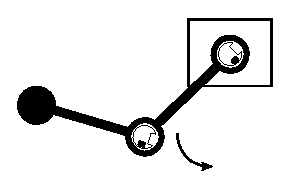
\includegraphics[width=.75\linewidth]{graphics/double_pendulum}
	\end{figure}
\end{frame}
\note{Another test was conducted where the double pendulum assembly was attached to the cart. The angles of the first joint were measured while letting it move freely after dropping it.}

\begin{frame}[c]\frametitle{Test of Double Pendulum}
    \begin{figure}[h]
		\centering
		% This file was created by matlab2tikz.
%
%The latest updates can be retrieved from
%  http://www.mathworks.com/matlabcentral/fileexchange/22022-matlab2tikz-matlab2tikz
%where you can also make suggestions and rate matlab2tikz.
%
\definecolor{mycolor1}{rgb}{0.00000,0.44700,0.74100}%
%
\begin{tikzpicture}

\begin{axis}[%
width=.8\textwidth,
height=2in,
at={(0.758in,0.481in)},
scale only axis,
xmin=66000,
xmax=90000,
xlabel style={font=\color{white!15!black}},
xlabel={Time [us]},
ymin=3000,
ymax=6500,
ylabel style={font=\color{white!15!black}},
ylabel={Angle [ticks]},
axis background/.style={fill=white},
title style={font=\bfseries},
title={Joint Angle},
axis x line*=bottom,
axis y line*=left
]
\addplot[only marks, mark=*, mark options={}, mark size=0.5000pt, draw=mycolor1] table[row sep=crcr]{%
x	y\\
56874	4676\\
56877	4600\\
56879	4600\\
56881	4600\\
56882	4600\\
56884	4600\\
56885	4600\\
56887	4600\\
56888	4600\\
56889	4600\\
56890	4600\\
56891	4600\\
56893	4600\\
56894	4600\\
56895	4600\\
56897	4600\\
56899	4600\\
56900	4600\\
56901	4600\\
56902	4600\\
56903	4600\\
56905	4600\\
56907	4600\\
56908	4600\\
56912	4600\\
56913	4600\\
56915	4600\\
56916	4600\\
56917	4600\\
56918	4600\\
56919	4600\\
56921	4600\\
56922	4600\\
56924	4600\\
56927	4600\\
56928	4600\\
56930	4600\\
56931	4600\\
56936	4600\\
56938	4600\\
56939	4600\\
56940	4600\\
56941	4600\\
56943	4600\\
56944	4600\\
56945	4600\\
56946	4600\\
56947	4600\\
56948	4600\\
56949	4600\\
56950	4600\\
56951	4600\\
56952	4600\\
56953	4600\\
56954	4600\\
56956	4600\\
56957	4600\\
56958	4600\\
56959	4600\\
56960	4600\\
56961	4600\\
56963	4600\\
56964	4600\\
56966	4600\\
56967	4600\\
56968	4600\\
56969	4600\\
56971	4600\\
56972	4600\\
56973	4600\\
56974	4600\\
56975	4600\\
56977	4600\\
56978	4600\\
56980	4600\\
56981	4600\\
56983	4600\\
56984	4600\\
56985	4600\\
56986	4600\\
56987	4600\\
56988	4600\\
56989	4600\\
56990	4600\\
56991	4600\\
56992	4600\\
56993	4600\\
56995	4600\\
56997	4600\\
56998	4600\\
56999	4600\\
57000	4600\\
57002	4600\\
57003	4600\\
57005	4600\\
57006	4600\\
57009	4600\\
57010	4600\\
57011	4600\\
57012	4600\\
57013	4600\\
57014	4600\\
57015	4600\\
57016	4600\\
57017	4600\\
57019	4600\\
57020	4600\\
57022	4600\\
57023	4600\\
57025	4600\\
57026	4600\\
57029	4600\\
57030	4600\\
57031	4600\\
57032	4600\\
57033	4600\\
57034	4600\\
57035	4600\\
57036	4600\\
57037	4600\\
57038	4600\\
57039	4600\\
57040	4600\\
57041	4600\\
57042	4600\\
57043	4600\\
57044	4600\\
57045	4600\\
57046	4600\\
57047	4600\\
57048	4600\\
57050	4600\\
57051	4600\\
57052	4600\\
57053	4600\\
57054	4600\\
57056	4600\\
57057	4600\\
57058	4600\\
57060	4600\\
57062	4600\\
57063	4600\\
57064	4600\\
57065	4600\\
57066	4600\\
57067	4600\\
57068	4600\\
57069	4600\\
57070	4600\\
57072	4600\\
57074	4600\\
57075	4600\\
57076	4600\\
57077	4600\\
57078	4600\\
57080	4600\\
57081	4600\\
57082	4600\\
57083	4600\\
57084	4600\\
57085	4600\\
57086	4600\\
57087	4600\\
57090	4600\\
57091	4600\\
57093	4600\\
57094	4600\\
57095	4600\\
57096	4600\\
57097	4600\\
57098	4600\\
57101	4600\\
57102	4600\\
57104	4600\\
57105	4600\\
57106	4600\\
57107	4600\\
57108	4600\\
57109	4600\\
57110	4600\\
57111	4600\\
57112	4600\\
57113	4600\\
57114	4600\\
57115	4600\\
57116	4600\\
57119	4600\\
57121	4600\\
57122	4600\\
57124	4600\\
57125	4600\\
57127	4600\\
57129	4600\\
57131	4600\\
57132	4600\\
57133	4600\\
57134	4600\\
57135	4600\\
57136	4600\\
57137	4600\\
57138	4600\\
57139	4600\\
57140	4600\\
57141	4600\\
57145	4600\\
57146	4600\\
57147	4600\\
57148	4600\\
57149	4600\\
57151	4600\\
57152	4600\\
57153	4600\\
57154	4600\\
57155	4600\\
57156	4600\\
57160	4600\\
57161	4600\\
57162	4600\\
57163	4600\\
57164	4600\\
57166	4600\\
57167	4600\\
57168	4600\\
57169	4600\\
57171	4600\\
57172	4600\\
57174	4600\\
57176	4600\\
57177	4600\\
57179	4600\\
57180	4600\\
57182	4600\\
57183	4600\\
57185	4600\\
57186	4600\\
57188	4600\\
57189	4600\\
57190	4600\\
57191	4600\\
57193	4600\\
57194	4600\\
57195	4600\\
57196	4600\\
57197	4600\\
57198	4600\\
57199	4600\\
57200	4600\\
57201	4600\\
57203	4600\\
57204	4600\\
57205	4600\\
57209	4600\\
57210	4600\\
57211	4600\\
57212	4600\\
57213	4600\\
57214	4600\\
57215	4600\\
57216	4600\\
57217	4600\\
57219	4600\\
57220	4600\\
57222	4600\\
57223	4600\\
57224	4600\\
57226	4600\\
57227	4600\\
57228	4600\\
57229	4600\\
57231	4600\\
57234	4600\\
57236	4600\\
57238	4600\\
57239	4600\\
57240	4600\\
57241	4600\\
57242	4600\\
57243	4600\\
57244	4600\\
57245	4600\\
57246	4600\\
57247	4600\\
57248	4600\\
57249	4600\\
57251	4600\\
57252	4600\\
57253	4600\\
57254	4600\\
57256	4600\\
57257	4600\\
57259	4600\\
57260	4600\\
57261	4600\\
57262	4600\\
57264	4600\\
57265	4600\\
57267	4600\\
57268	4600\\
57269	4600\\
57270	4600\\
57271	4600\\
57272	4600\\
57273	4600\\
57275	4600\\
57276	4600\\
57277	4600\\
57278	4600\\
57279	4600\\
57280	4600\\
57281	4600\\
57282	4600\\
57283	4600\\
57284	4600\\
57285	4600\\
57287	4600\\
57289	4600\\
57292	4600\\
57293	4600\\
57294	4600\\
57295	4600\\
57296	4600\\
57298	4600\\
57300	4600\\
57301	4600\\
57303	4600\\
57304	4600\\
57306	4600\\
57307	4600\\
57308	4600\\
57309	4600\\
57311	4600\\
57312	4600\\
57314	4600\\
57316	4600\\
57319	4600\\
57321	4600\\
57322	4600\\
57323	4600\\
57324	4600\\
57325	4600\\
57326	4600\\
57328	4600\\
57329	4600\\
57330	4600\\
57331	4600\\
57332	4600\\
57333	4600\\
57334	4600\\
57335	4600\\
57336	4600\\
57337	4600\\
57338	4600\\
57339	4600\\
57340	4600\\
57341	4600\\
57342	4600\\
57343	4600\\
57344	4600\\
57345	4600\\
57346	4600\\
57347	4600\\
57348	4600\\
57349	4600\\
57350	4600\\
57351	4600\\
57352	4600\\
57354	4600\\
57355	4600\\
57356	4600\\
57357	4600\\
57358	4600\\
57360	4600\\
57361	4600\\
57362	4600\\
57363	4600\\
57366	4600\\
57367	4600\\
57368	4600\\
57369	4600\\
57370	4600\\
57373	4600\\
57374	4600\\
57375	4600\\
57376	4600\\
57377	4600\\
57378	4600\\
57380	4600\\
57382	4600\\
57383	4600\\
57384	4600\\
57386	4600\\
57388	4600\\
57389	4600\\
57390	4600\\
57391	4600\\
57392	4600\\
57393	4600\\
57394	4600\\
57396	4600\\
57400	4600\\
57401	4600\\
57403	4600\\
57404	4600\\
57405	4600\\
57406	4600\\
57407	4600\\
57408	4600\\
57409	4600\\
57410	4600\\
57411	4600\\
57412	4600\\
57413	4600\\
57414	4600\\
57415	4600\\
57416	4600\\
57417	4600\\
57418	4600\\
57419	4600\\
57420	4600\\
57422	4600\\
57423	4600\\
57425	4600\\
57427	4600\\
57428	4600\\
57430	4600\\
57431	4600\\
57432	4600\\
57433	4600\\
57434	4600\\
57435	4600\\
57436	4600\\
57437	4600\\
57438	4600\\
57439	4600\\
57440	4600\\
57441	4600\\
57442	4600\\
57443	4600\\
57444	4600\\
57445	4600\\
57446	4600\\
57447	4600\\
57448	4600\\
57449	4600\\
57450	4600\\
57451	4600\\
57453	4600\\
57454	4600\\
57455	4600\\
57456	4600\\
57457	4600\\
57459	4600\\
57460	4600\\
57461	4600\\
57462	4600\\
57463	4600\\
57465	4600\\
57466	4600\\
57467	4600\\
57468	4600\\
57469	4600\\
57471	4600\\
57472	4600\\
57473	4600\\
57474	4600\\
57475	4600\\
57476	4600\\
57477	4600\\
57478	4600\\
57479	4600\\
57480	4600\\
57483	4600\\
57484	4600\\
57485	4600\\
57486	4600\\
57488	4600\\
57489	4600\\
57490	4600\\
57491	4600\\
57492	4600\\
57494	4600\\
57495	4600\\
57496	4600\\
57497	4600\\
57498	4600\\
57500	4600\\
57501	4600\\
57502	4600\\
57503	4600\\
57506	4600\\
57507	4600\\
57508	4600\\
57509	4600\\
57510	4600\\
57511	4600\\
57512	4600\\
57513	4600\\
57514	4600\\
57515	4600\\
57517	4600\\
57518	4600\\
57519	4600\\
57520	4600\\
57521	4600\\
57523	4600\\
57524	4600\\
57525	4600\\
57526	4600\\
57527	4600\\
57528	4600\\
57529	4600\\
57530	4600\\
57531	4600\\
57532	4600\\
57535	4600\\
57536	4600\\
57537	4600\\
57538	4600\\
57540	4600\\
57541	4600\\
57542	4600\\
57543	4600\\
57544	4600\\
57545	4600\\
57546	4600\\
57547	4600\\
57548	4600\\
57549	4600\\
57550	4600\\
57552	4600\\
57553	4600\\
57554	4600\\
57555	4600\\
57556	4600\\
57557	4600\\
57558	4600\\
57559	4600\\
57560	4600\\
57561	4600\\
57564	4600\\
57565	4600\\
57566	4600\\
57567	4600\\
57568	4600\\
57569	4600\\
57570	4600\\
57571	4600\\
57572	4600\\
57574	4600\\
57575	4600\\
57576	4600\\
57577	4600\\
57578	4600\\
57581	4600\\
57582	4600\\
57583	4600\\
57584	4600\\
57587	4600\\
57588	4600\\
57589	4600\\
57590	4600\\
57592	4600\\
57593	4600\\
57594	4600\\
57595	4600\\
57596	4600\\
57598	4600\\
57599	4600\\
57600	4600\\
57601	4600\\
57602	4600\\
57604	4600\\
57605	4600\\
57606	4600\\
57607	4600\\
57608	4600\\
57610	4600\\
57611	4600\\
57612	4600\\
57613	4600\\
57614	4600\\
57616	4600\\
57617	4600\\
57618	4600\\
57619	4600\\
57621	4600\\
57622	4600\\
57623	4600\\
57624	4600\\
57625	4600\\
57627	4600\\
57628	4600\\
57629	4600\\
57630	4600\\
57631	4600\\
57633	4600\\
57634	4600\\
57635	4600\\
57636	4600\\
57637	4600\\
57639	4600\\
57640	4600\\
57641	4600\\
57642	4600\\
57645	4600\\
57646	4600\\
57648	4600\\
57649	4600\\
57650	4600\\
57651	4600\\
57652	4600\\
57656	4600\\
57658	4600\\
57659	4600\\
57661	4600\\
57662	4600\\
57663	4600\\
57664	4600\\
57667	4600\\
57669	4600\\
57671	4600\\
57672	4600\\
57674	4600\\
57675	4600\\
57676	4600\\
57677	4600\\
57678	4600\\
57679	4600\\
57680	4600\\
57681	4600\\
57683	4600\\
57684	4600\\
57686	4600\\
57687	4600\\
57688	4600\\
57689	4600\\
57690	4600\\
57691	4600\\
57692	4600\\
57693	4600\\
57694	4600\\
57695	4600\\
57696	4600\\
57697	4600\\
57698	4600\\
57699	4600\\
57700	4600\\
57702	4600\\
57704	4600\\
57705	4600\\
57706	4600\\
57707	4600\\
57708	4600\\
57709	4600\\
57710	4600\\
57711	4600\\
57712	4600\\
57713	4600\\
57714	4600\\
57716	4600\\
57718	4600\\
57719	4600\\
57721	4600\\
57722	4600\\
57723	4600\\
57724	4600\\
57725	4600\\
57726	4600\\
57727	4600\\
57728	4600\\
57730	4600\\
57731	4600\\
57732	4600\\
57733	4600\\
57734	4600\\
57735	4600\\
57736	4600\\
57737	4600\\
57738	4600\\
57739	4600\\
57740	4600\\
57741	4600\\
57742	4600\\
57743	4600\\
57744	4600\\
57745	4600\\
57747	4600\\
57748	4600\\
57749	4600\\
57750	4600\\
57751	4600\\
57753	4600\\
57754	4600\\
57755	4600\\
57756	4600\\
57757	4600\\
57759	4600\\
57760	4600\\
57761	4600\\
57762	4600\\
57763	4600\\
57765	4600\\
57766	4600\\
57767	4600\\
57768	4600\\
57770	4600\\
57771	4600\\
57772	4600\\
57773	4600\\
57774	4600\\
57776	4600\\
57777	4600\\
57778	4600\\
57779	4600\\
57780	4600\\
57782	4600\\
57783	4600\\
57784	4600\\
57785	4600\\
57786	4600\\
57788	4600\\
57789	4600\\
57790	4600\\
57791	4600\\
57792	4600\\
57793	4600\\
57794	4600\\
57795	4600\\
57796	4600\\
57797	4600\\
57800	4600\\
57801	4600\\
57802	4600\\
57803	4600\\
57806	4600\\
57807	4600\\
57808	4600\\
57809	4600\\
57810	4600\\
57811	4600\\
57812	4600\\
57813	4600\\
57814	4600\\
57815	4600\\
57817	4600\\
57818	4600\\
57819	4600\\
57820	4600\\
57821	4600\\
57823	4600\\
57824	4600\\
57825	4600\\
57826	4600\\
57830	4600\\
57831	4600\\
57833	4600\\
57834	4600\\
57835	4600\\
57836	4600\\
57839	4600\\
57840	4600\\
57841	4600\\
57842	4600\\
57843	4600\\
57845	4600\\
57846	4600\\
57848	4600\\
57849	4600\\
57850	4600\\
57851	4600\\
57852	4600\\
57854	4600\\
57855	4600\\
57856	4600\\
57857	4600\\
57859	4600\\
57860	4600\\
57861	4600\\
57863	4600\\
57864	4600\\
57865	4600\\
57866	4600\\
57867	4600\\
57868	4600\\
57871	4600\\
57873	4600\\
57874	4600\\
57875	4600\\
57876	4600\\
57877	4600\\
57878	4600\\
57879	4600\\
57880	4600\\
57881	4600\\
57882	4600\\
57883	4600\\
57884	4600\\
57885	4600\\
57886	4600\\
57887	4600\\
57888	4600\\
57889	4600\\
57890	4600\\
57891	4600\\
57892	4600\\
57893	4600\\
57894	4600\\
57895	4600\\
57896	4600\\
57897	4600\\
57898	4600\\
57899	4600\\
57900	4600\\
57901	4600\\
57902	4600\\
57903	4600\\
57904	4600\\
57906	4600\\
57907	4600\\
57908	4600\\
57909	4600\\
57910	4600\\
57911	4600\\
57912	4600\\
57913	4600\\
57914	4600\\
57915	4600\\
57917	4600\\
57918	4600\\
57919	4600\\
57920	4600\\
57923	4600\\
57924	4600\\
57925	4600\\
57926	4600\\
57927	4600\\
57929	4600\\
57930	4600\\
57931	4600\\
57932	4600\\
57935	4600\\
57936	4600\\
57937	4600\\
57938	4600\\
57939	4600\\
57941	4600\\
57942	4600\\
57943	4600\\
57944	4600\\
57946	4600\\
57947	4600\\
57948	4600\\
57949	4600\\
57950	4600\\
57951	4600\\
57952	4600\\
57953	4600\\
57954	4600\\
57955	4600\\
57956	4600\\
57958	4600\\
57959	4600\\
57960	4600\\
57961	4600\\
57962	4600\\
57963	4600\\
57964	4600\\
57965	4600\\
57966	4600\\
57967	4600\\
57969	4600\\
57970	4600\\
57971	4600\\
57972	4600\\
57975	4600\\
57976	4600\\
57977	4600\\
57978	4600\\
57979	4600\\
57981	4600\\
57982	4600\\
57983	4600\\
57984	4600\\
57985	4600\\
57987	4600\\
57988	4600\\
57989	4600\\
57990	4600\\
57991	4600\\
57992	4600\\
57993	4600\\
57994	4600\\
57995	4600\\
57996	4600\\
57998	4600\\
57999	4600\\
58000	4600\\
58001	4600\\
58004	4600\\
58005	4600\\
58006	4600\\
58007	4600\\
58008	4600\\
58010	4600\\
58011	4600\\
58012	4600\\
58013	4600\\
58014	4600\\
58015	4600\\
58016	4600\\
58017	4600\\
58018	4600\\
58019	4600\\
58021	4600\\
58022	4600\\
58023	4600\\
58024	4600\\
58025	4600\\
58027	4600\\
58028	4600\\
58029	4600\\
58030	4600\\
58033	4600\\
58034	4600\\
58035	4600\\
58036	4600\\
58037	4600\\
58039	4600\\
58040	4600\\
58041	4600\\
58042	4600\\
58043	4600\\
58045	4600\\
58046	4600\\
58047	4600\\
58048	4600\\
58051	4600\\
58052	4600\\
58053	4600\\
58054	4600\\
58056	4600\\
58057	4600\\
58058	4600\\
58059	4600\\
58060	4600\\
58062	4600\\
58063	4600\\
58064	4600\\
58065	4600\\
58066	4600\\
58068	4600\\
58069	4600\\
58070	4600\\
58071	4600\\
58072	4600\\
58074	4600\\
58075	4600\\
58076	4600\\
58077	4600\\
58079	4600\\
58080	4600\\
58081	4600\\
58082	4600\\
58083	4600\\
58085	4600\\
58086	4600\\
58087	4600\\
58088	4600\\
58089	4600\\
58091	4600\\
58092	4600\\
58093	4600\\
58094	4600\\
58095	4600\\
58097	4600\\
58098	4600\\
58099	4600\\
58100	4600\\
58102	4600\\
58103	4600\\
58104	4600\\
58105	4600\\
58106	4600\\
58108	4600\\
58109	4600\\
58110	4600\\
58111	4600\\
58112	4600\\
58114	4600\\
58115	4600\\
58116	4600\\
58117	4600\\
58118	4600\\
58120	4600\\
58121	4600\\
58122	4600\\
58123	4600\\
58124	4600\\
58126	4600\\
58127	4600\\
58128	4600\\
58129	4600\\
58131	4600\\
58132	4600\\
58133	4600\\
58134	4600\\
58135	4600\\
58137	4600\\
58138	4600\\
58139	4600\\
58140	4600\\
58141	4600\\
58143	4600\\
58144	4600\\
58145	4600\\
58146	4600\\
58147	4600\\
58149	4600\\
58150	4600\\
58151	4600\\
58152	4600\\
58153	4600\\
58155	4600\\
58156	4600\\
58157	4600\\
58158	4600\\
58160	4600\\
58161	4600\\
58162	4600\\
58163	4600\\
58164	4600\\
58165	4600\\
58166	4600\\
58167	4600\\
58168	4600\\
58169	4600\\
58170	4600\\
58172	4600\\
58173	4600\\
58174	4600\\
58175	4600\\
58176	4600\\
58178	4600\\
58179	4600\\
58180	4600\\
58181	4600\\
58183	4600\\
58184	4600\\
58185	4600\\
58186	4600\\
58187	4600\\
58190	4600\\
58191	4600\\
58192	4600\\
58193	4600\\
58195	4600\\
58196	4600\\
58197	4600\\
58198	4600\\
58199	4600\\
58201	4600\\
58202	4600\\
58203	4600\\
58204	4600\\
58205	4600\\
58207	4600\\
58208	4600\\
58209	4600\\
58210	4600\\
58212	4600\\
58213	4600\\
58214	4600\\
58215	4600\\
58216	4600\\
58218	4600\\
58219	4600\\
58220	4600\\
58221	4600\\
58222	4600\\
58224	4600\\
58225	4600\\
58226	4600\\
58227	4600\\
58228	4600\\
58230	4600\\
58231	4600\\
58232	4600\\
58233	4600\\
58234	4600\\
58235	4600\\
58236	4600\\
58237	4600\\
58238	4600\\
58239	4600\\
58241	4600\\
58242	4600\\
58243	4600\\
58244	4600\\
58245	4600\\
58248	4600\\
58249	4600\\
58250	4600\\
58251	4600\\
58253	4600\\
58254	4600\\
58255	4600\\
58256	4600\\
58257	4600\\
58259	4600\\
58260	4600\\
58261	4600\\
58262	4600\\
58263	4600\\
58265	4600\\
58266	4600\\
58267	4600\\
58268	4600\\
58269	4600\\
58271	4600\\
58272	4600\\
58273	4600\\
58274	4600\\
58275	4600\\
58276	4600\\
58277	4600\\
58278	4600\\
58279	4600\\
58280	4600\\
58282	4600\\
58283	4600\\
58284	4600\\
58285	4600\\
58286	4600\\
58288	4600\\
58289	4600\\
58290	4600\\
58291	4600\\
58292	4600\\
58294	4600\\
58295	4600\\
58296	4600\\
58297	4600\\
58300	4600\\
58301	4600\\
58302	4600\\
58303	4600\\
58305	4600\\
58306	4600\\
58307	4600\\
58308	4600\\
58309	4600\\
58311	4600\\
58312	4600\\
58313	4600\\
58314	4600\\
58315	4600\\
58317	4600\\
58318	4600\\
58319	4600\\
58320	4600\\
58322	4600\\
58323	4600\\
58324	4600\\
58325	4600\\
58326	4600\\
58328	4600\\
58329	4600\\
58330	4600\\
58331	4600\\
58332	4600\\
58334	4600\\
58335	4600\\
58336	4600\\
58337	4600\\
58338	4600\\
58340	4600\\
58341	4600\\
58342	4600\\
58343	4600\\
58344	4600\\
58346	4600\\
58347	4600\\
58348	4600\\
58349	4600\\
58351	4600\\
58352	4600\\
58353	4600\\
58354	4600\\
58355	4600\\
58356	4600\\
58358	4600\\
58359	4600\\
58360	4600\\
58361	4600\\
58362	4600\\
58363	4600\\
58364	4600\\
58365	4600\\
58366	4600\\
58367	4600\\
58369	4600\\
58370	4600\\
58371	4600\\
58372	4600\\
58373	4600\\
58375	4600\\
58376	4600\\
58377	4600\\
58378	4600\\
58381	4600\\
58382	4600\\
58383	4600\\
58384	4600\\
58386	4600\\
58387	4600\\
58388	4600\\
58389	4600\\
58390	4600\\
58392	4600\\
58393	4600\\
58394	4600\\
58395	4600\\
58396	4600\\
58397	4600\\
58398	4600\\
58399	4600\\
58400	4600\\
58401	4600\\
58402	4600\\
58403	4600\\
58404	4600\\
58405	4600\\
58406	4600\\
58407	4600\\
58410	4600\\
58411	4600\\
58412	4600\\
58413	4600\\
58415	4600\\
58416	4600\\
58417	4600\\
58418	4600\\
58419	4600\\
58420	4600\\
58421	4600\\
58422	4600\\
58423	4600\\
58424	4600\\
58427	4600\\
58428	4600\\
58429	4600\\
58430	4600\\
58431	4600\\
58433	4600\\
58434	4600\\
58435	4600\\
58436	4600\\
58439	4600\\
58440	4600\\
58441	4600\\
58442	4600\\
58444	4600\\
58445	4600\\
58446	4600\\
58447	4600\\
58448	4600\\
58450	4600\\
58451	4600\\
58452	4600\\
58453	4600\\
58454	4600\\
58456	4600\\
58457	4600\\
58458	4600\\
58459	4600\\
58461	4600\\
58462	4600\\
58463	4600\\
58464	4600\\
58465	4600\\
58467	4600\\
58468	4600\\
58469	4600\\
58470	4600\\
58471	4600\\
58473	4600\\
58474	4600\\
58475	4600\\
58476	4600\\
58477	4600\\
58479	4600\\
58480	4600\\
58481	4600\\
58482	4600\\
58483	4600\\
58485	4600\\
58486	4600\\
58487	4600\\
58488	4600\\
58490	4600\\
58491	4600\\
58492	4600\\
58493	4600\\
58494	4600\\
58496	4600\\
58497	4600\\
58498	4600\\
58499	4600\\
58500	4600\\
58502	4600\\
58503	4600\\
58504	4600\\
58505	4600\\
58506	4600\\
58507	4600\\
58508	4600\\
58509	4600\\
58510	4600\\
58511	4600\\
58512	4600\\
58514	4600\\
58515	4600\\
58516	4600\\
58517	4600\\
58518	4600\\
58519	4600\\
58520	4600\\
58521	4600\\
58522	4600\\
58523	4600\\
58526	4600\\
58527	4600\\
58528	4600\\
58529	4600\\
58531	4600\\
58532	4600\\
58533	4600\\
58534	4600\\
58535	4600\\
58537	4600\\
58538	4600\\
58539	4600\\
58540	4600\\
58541	4600\\
58543	4600\\
58544	4600\\
58545	4600\\
58546	4600\\
58549	4600\\
58550	4600\\
58551	4600\\
58552	4600\\
58554	4600\\
58555	4600\\
58556	4600\\
58557	4600\\
58558	4600\\
58560	4600\\
58561	4600\\
58562	4600\\
58563	4600\\
58564	4600\\
58566	4600\\
58567	4600\\
58568	4600\\
58569	4600\\
58570	4600\\
58572	4600\\
58573	4600\\
58574	4600\\
58575	4600\\
58578	4600\\
58579	4600\\
58580	4600\\
58581	4600\\
58583	4600\\
58584	4600\\
58586	4600\\
58587	4600\\
58589	4600\\
58591	4600\\
58592	4600\\
58595	4600\\
58597	4600\\
58598	4600\\
58599	4600\\
58600	4600\\
58601	4600\\
58602	4600\\
58607	4600\\
58608	4600\\
58609	4600\\
58610	4600\\
58611	4600\\
58612	4600\\
58613	4600\\
58614	4600\\
58620	4600\\
58621	4600\\
58622	4600\\
58623	4600\\
58625	4600\\
58626	4600\\
58629	4600\\
58631	4600\\
58632	4600\\
58633	4600\\
58634	4600\\
58635	4600\\
58637	4600\\
58638	4600\\
58640	4600\\
58641	4600\\
58642	4600\\
58645	4600\\
58646	4600\\
58648	4600\\
58649	4600\\
58650	4600\\
58651	4600\\
58652	4600\\
58653	4600\\
58654	4600\\
58656	4600\\
58657	4600\\
58658	4600\\
58660	4600\\
58662	4600\\
58663	4600\\
58666	4600\\
58668	4600\\
58670	4600\\
58673	4600\\
58675	4600\\
58676	4600\\
58678	4600\\
58679	4600\\
58680	4600\\
58681	4600\\
58683	4600\\
58684	4600\\
58685	4600\\
58686	4600\\
58687	4600\\
58690	4600\\
58691	4600\\
58693	4600\\
58694	4600\\
58695	4600\\
58696	4600\\
58698	4600\\
58699	4600\\
58701	4600\\
58702	4600\\
58703	4600\\
58704	4600\\
58705	4600\\
58706	4600\\
58707	4600\\
58708	4600\\
58709	4600\\
58710	4600\\
58715	4600\\
58717	4600\\
58718	4600\\
58719	4600\\
58721	4600\\
58722	4600\\
58723	4600\\
58725	4600\\
58726	4600\\
58727	4600\\
58733	4600\\
58734	4600\\
58735	4600\\
58736	4600\\
58737	4600\\
58738	4600\\
58739	4600\\
58741	4600\\
58742	4600\\
58743	4600\\
58744	4600\\
58747	4600\\
58748	4600\\
58749	4600\\
58750	4600\\
58751	4600\\
58753	4600\\
58754	4600\\
58755	4600\\
58756	4600\\
58757	4600\\
58758	4600\\
58759	4600\\
58760	4600\\
58761	4600\\
58765	4600\\
58767	4600\\
58768	4600\\
58769	4600\\
58770	4600\\
58773	4600\\
58775	4600\\
58776	4600\\
58777	4600\\
58778	4600\\
58779	4600\\
58780	4600\\
58781	4600\\
58782	4600\\
58783	4600\\
58784	4600\\
58785	4600\\
58787	4600\\
58789	4600\\
58790	4600\\
58791	4600\\
58792	4600\\
58793	4600\\
58794	4600\\
58795	4600\\
58796	4600\\
58797	4600\\
58800	4600\\
58801	4600\\
58803	4600\\
58804	4600\\
58806	4600\\
58807	4600\\
58808	4600\\
58809	4600\\
58810	4600\\
58812	4600\\
58814	4600\\
58815	4600\\
58816	4600\\
58817	4600\\
58818	4600\\
58819	4600\\
58821	4600\\
58822	4600\\
58823	4600\\
58824	4600\\
58825	4600\\
58827	4600\\
58828	4600\\
58830	4600\\
58831	4600\\
58833	4600\\
58835	4600\\
58836	4600\\
58838	4600\\
58839	4600\\
58840	4600\\
58841	4600\\
58842	4600\\
58843	4600\\
58845	4600\\
58846	4600\\
58847	4600\\
58848	4600\\
58849	4600\\
58850	4600\\
58851	4600\\
58852	4600\\
58853	4600\\
58854	4600\\
58855	4600\\
58857	4600\\
58858	4600\\
58859	4600\\
58860	4600\\
58861	4600\\
58863	4600\\
58864	4600\\
58866	4600\\
58867	4600\\
58869	4600\\
58870	4600\\
58871	4600\\
58872	4600\\
58873	4600\\
58874	4600\\
58875	4600\\
58876	4600\\
58878	4600\\
58879	4600\\
58880	4600\\
58881	4600\\
58883	4600\\
58885	4600\\
58886	4600\\
58887	4600\\
58888	4600\\
58889	4600\\
58891	4600\\
58892	4600\\
58894	4600\\
58896	4600\\
58897	4600\\
58898	4600\\
58899	4600\\
58902	4600\\
58904	4600\\
58905	4600\\
58907	4600\\
58909	4600\\
58910	4600\\
58911	4600\\
58912	4600\\
58913	4600\\
58914	4600\\
58915	4600\\
58916	4600\\
58918	4600\\
58919	4600\\
58920	4600\\
58923	4600\\
58924	4600\\
58925	4600\\
58927	4600\\
58929	4600\\
58930	4600\\
58931	4600\\
58932	4600\\
58933	4600\\
58934	4600\\
58935	4600\\
58936	4600\\
58938	4600\\
58940	4600\\
58941	4600\\
58942	4600\\
58943	4600\\
58944	4600\\
58945	4600\\
58946	4600\\
58947	4600\\
58948	4600\\
58949	4600\\
58950	4600\\
58951	4600\\
58952	4600\\
58953	4600\\
58955	4600\\
58956	4600\\
58958	4600\\
58959	4600\\
58960	4600\\
58961	4600\\
58962	4600\\
58963	4600\\
58964	4600\\
58965	4600\\
58966	4600\\
58967	4600\\
58969	4600\\
58970	4600\\
58971	4600\\
58972	4600\\
58973	4600\\
58974	4600\\
58975	4600\\
58976	4600\\
58978	4600\\
58979	4600\\
58980	4600\\
58981	4600\\
58982	4600\\
58983	4600\\
58984	4600\\
58985	4600\\
58986	4600\\
58987	4600\\
58988	4600\\
58990	4600\\
58991	4600\\
58992	4600\\
58993	4600\\
58994	4600\\
58996	4600\\
58997	4600\\
58998	4600\\
58999	4600\\
59000	4600\\
59002	4600\\
59003	4600\\
59004	4600\\
59005	4600\\
59007	4600\\
59008	4600\\
59009	4600\\
59010	4600\\
59011	4600\\
59013	4600\\
59014	4600\\
59015	4600\\
59016	4600\\
59017	4600\\
59019	4600\\
59020	4600\\
59021	4600\\
59022	4600\\
59023	4600\\
59025	4600\\
59026	4600\\
59027	4600\\
59028	4600\\
59029	4600\\
59031	4600\\
59032	4600\\
59033	4600\\
59034	4600\\
59037	4600\\
59038	4600\\
59039	4600\\
59040	4600\\
59042	4600\\
59044	4600\\
59045	4600\\
59046	4600\\
59047	4600\\
59048	4600\\
59050	4600\\
59052	4600\\
59053	4600\\
59057	4600\\
59058	4600\\
59059	4600\\
59060	4600\\
59062	4600\\
59063	4600\\
59064	4600\\
59065	4600\\
59066	4600\\
59067	4600\\
59069	4600\\
59071	4600\\
59072	4600\\
59073	4600\\
59075	4600\\
59076	4600\\
59077	4600\\
59078	4600\\
59079	4600\\
59080	4600\\
59081	4600\\
59082	4600\\
59083	4600\\
59084	4600\\
59086	4600\\
59088	4600\\
59089	4600\\
59090	4600\\
59092	4600\\
59096	4600\\
59097	4600\\
59099	4600\\
59100	4600\\
59101	4600\\
59102	4600\\
59103	4600\\
59104	4600\\
59105	4600\\
59107	4600\\
59108	4600\\
59109	4600\\
59111	4600\\
59113	4600\\
59114	4600\\
59115	4600\\
59116	4600\\
59117	4600\\
59118	4600\\
59120	4600\\
59123	4600\\
59124	4600\\
59125	4600\\
59130	4600\\
59131	4600\\
59133	4600\\
59134	4600\\
59136	4600\\
59138	4600\\
59139	4600\\
59142	4600\\
59143	4600\\
59144	4600\\
59145	4600\\
59146	4600\\
59147	4600\\
59149	4600\\
59150	4600\\
59151	4600\\
59152	4600\\
59153	4600\\
59154	4600\\
59156	4600\\
59157	4600\\
59160	4600\\
59161	4600\\
59162	4600\\
59163	4600\\
59164	4600\\
59165	4600\\
59167	4600\\
59169	4600\\
59170	4600\\
59171	4600\\
59174	4600\\
59175	4600\\
59176	4600\\
59178	4600\\
59179	4600\\
59180	4600\\
59183	4600\\
59184	4600\\
59186	4600\\
59187	4600\\
59189	4600\\
59190	4600\\
59192	4600\\
59193	4600\\
59194	4600\\
59195	4600\\
59196	4600\\
59198	4600\\
59199	4600\\
59200	4600\\
59201	4600\\
59202	4600\\
59204	4600\\
59206	4600\\
59207	4600\\
59210	4600\\
59211	4600\\
59212	4600\\
59213	4600\\
59215	4600\\
59216	4600\\
59217	4600\\
59218	4600\\
59219	4600\\
59221	4600\\
59222	4600\\
59227	4600\\
59228	4600\\
59229	4600\\
59230	4600\\
59231	4600\\
59232	4600\\
59233	4600\\
59234	4600\\
59235	4600\\
59236	4600\\
59237	4600\\
59240	4600\\
59242	4600\\
59244	4600\\
59245	4600\\
59247	4600\\
59248	4600\\
59249	4600\\
59250	4600\\
59251	4600\\
59253	4600\\
59254	4600\\
59256	4600\\
59257	4600\\
59258	4600\\
59259	4600\\
59261	4600\\
59262	4600\\
59265	4600\\
59267	4600\\
59268	4600\\
59269	4600\\
59270	4600\\
59271	4600\\
59273	4600\\
59275	4600\\
59276	4600\\
59278	4600\\
59279	4600\\
59280	4600\\
59281	4600\\
59283	4600\\
59284	4600\\
59286	4600\\
59287	4600\\
59289	4600\\
59290	4600\\
59291	4600\\
59292	4600\\
59293	4600\\
59294	4600\\
59295	4600\\
59297	4600\\
59298	4600\\
59299	4600\\
59300	4600\\
59301	4600\\
59302	4600\\
59303	4600\\
59304	4600\\
59305	4600\\
59306	4600\\
59308	4600\\
59309	4600\\
59311	4600\\
59313	4600\\
59314	4600\\
59315	4600\\
59316	4600\\
59317	4600\\
59318	4600\\
59319	4600\\
59320	4600\\
59321	4600\\
59324	4600\\
59325	4600\\
59326	4600\\
59328	4600\\
59329	4600\\
59330	4600\\
59331	4600\\
59333	4600\\
59334	4600\\
59335	4600\\
59336	4600\\
59337	4600\\
59339	4600\\
59340	4600\\
59341	4600\\
59342	4600\\
59343	4600\\
59345	4600\\
59347	4600\\
59349	4600\\
59351	4600\\
59352	4600\\
59354	4600\\
59355	4600\\
59357	4600\\
59358	4600\\
59359	4600\\
59360	4600\\
59361	4600\\
59362	4600\\
59363	4600\\
59364	4600\\
59365	4600\\
59366	4600\\
59367	4600\\
59368	4600\\
59369	4600\\
59370	4600\\
59371	4600\\
59373	4600\\
59375	4600\\
59380	4600\\
59382	4600\\
59383	4600\\
59384	4600\\
59385	4600\\
59386	4600\\
59388	4600\\
59390	4600\\
59391	4600\\
59393	4600\\
59394	4600\\
59395	4600\\
59396	4600\\
59399	4600\\
59400	4600\\
59401	4600\\
59402	4600\\
59403	4600\\
59404	4600\\
59405	4600\\
59406	4600\\
59408	4600\\
59409	4600\\
59411	4600\\
59416	4600\\
59418	4600\\
59419	4600\\
59421	4600\\
59422	4600\\
59424	4600\\
59425	4600\\
59426	4600\\
59427	4600\\
59429	4600\\
59430	4600\\
59432	4600\\
59433	4600\\
59435	4600\\
59436	4600\\
59437	4600\\
59438	4600\\
59439	4600\\
59440	4600\\
59442	4600\\
59443	4600\\
59445	4600\\
59447	4600\\
59448	4600\\
59449	4600\\
59450	4600\\
59451	4600\\
59452	4600\\
59453	4600\\
59454	4600\\
59456	4600\\
59457	4600\\
59458	4600\\
59459	4600\\
59460	4600\\
59461	4600\\
59462	4600\\
59463	4600\\
59465	4600\\
59466	4600\\
59467	4600\\
59468	4600\\
59470	4600\\
59471	4600\\
59472	4600\\
59473	4600\\
59474	4600\\
59475	4600\\
59476	4600\\
59477	4600\\
59478	4600\\
59480	4600\\
59481	4600\\
59482	4600\\
59483	4600\\
59484	4600\\
59486	4600\\
59488	4600\\
59489	4600\\
59490	4600\\
59491	4600\\
59493	4600\\
59494	4600\\
59495	4600\\
59496	4600\\
59497	4600\\
59498	4600\\
59499	4600\\
59500	4600\\
59501	4600\\
59502	4600\\
59504	4600\\
59505	4600\\
59506	4600\\
59507	4600\\
59508	4600\\
59509	4600\\
59510	4600\\
59512	4600\\
59514	4600\\
59516	4600\\
59518	4600\\
59519	4600\\
59520	4600\\
59521	4600\\
59522	4600\\
59523	4600\\
59525	4600\\
59527	4600\\
59528	4600\\
59529	4600\\
59531	4600\\
59532	4600\\
59533	4600\\
59534	4600\\
59535	4600\\
59537	4600\\
59541	4600\\
59542	4600\\
59544	4600\\
59545	4600\\
59546	4600\\
59547	4600\\
59548	4600\\
59549	4600\\
59550	4600\\
59552	4600\\
59553	4600\\
59554	4600\\
59555	4600\\
59556	4600\\
59557	4600\\
59558	4600\\
59559	4600\\
59560	4600\\
59561	4600\\
59565	4600\\
59566	4600\\
59567	4600\\
59568	4600\\
59569	4600\\
59570	4600\\
59572	4600\\
59573	4600\\
59574	4600\\
59576	4600\\
59578	4600\\
59579	4600\\
59580	4600\\
59581	4600\\
59582	4600\\
59584	4600\\
59585	4600\\
59586	4600\\
59588	4600\\
59589	4600\\
59590	4600\\
59591	4600\\
59592	4600\\
59593	4600\\
59594	4600\\
59595	4600\\
59597	4600\\
59598	4600\\
59599	4600\\
59602	4600\\
59603	4600\\
59604	4600\\
59605	4600\\
59606	4600\\
59607	4600\\
59608	4600\\
59611	4600\\
59612	4600\\
59614	4600\\
59615	4600\\
59616	4600\\
59617	4600\\
59618	4600\\
59619	4600\\
59620	4600\\
59621	4600\\
59622	4600\\
59624	4600\\
59625	4600\\
59627	4600\\
59631	4600\\
59632	4600\\
59633	4600\\
59635	4600\\
59636	4600\\
59637	4600\\
59638	4600\\
59642	4600\\
59643	4600\\
59645	4600\\
59646	4600\\
59648	4600\\
59652	4600\\
59653	4600\\
59654	4600\\
59655	4600\\
59656	4600\\
59657	4600\\
59658	4600\\
59659	4600\\
59661	4600\\
59663	4600\\
59664	4600\\
59666	4600\\
59667	4600\\
59668	4600\\
59669	4600\\
59670	4600\\
59672	4600\\
59673	4600\\
59674	4600\\
59675	4600\\
59676	4600\\
59678	4600\\
59679	4600\\
59680	4600\\
59681	4600\\
59682	4600\\
59683	4600\\
59684	4600\\
59685	4600\\
59686	4600\\
59687	4600\\
59688	4600\\
59689	4600\\
59691	4600\\
59693	4600\\
59695	4600\\
59696	4600\\
59697	4600\\
59698	4600\\
59699	4600\\
59701	4600\\
59703	4600\\
59704	4600\\
59705	4600\\
59706	4600\\
59707	4600\\
59708	4600\\
59709	4600\\
59710	4600\\
59711	4600\\
59713	4600\\
59714	4600\\
59715	4600\\
59716	4600\\
59717	4600\\
59719	4600\\
59720	4600\\
59721	4600\\
59722	4600\\
59723	4600\\
59724	4600\\
59725	4600\\
59726	4600\\
59727	4600\\
59728	4600\\
59729	4600\\
59730	4600\\
59731	4600\\
59734	4600\\
59735	4600\\
59737	4600\\
59739	4600\\
59740	4600\\
59742	4600\\
59743	4600\\
59745	4600\\
59746	4600\\
59747	4600\\
59748	4600\\
59749	4600\\
59750	4600\\
59751	4600\\
59752	4600\\
59753	4600\\
59754	4600\\
59755	4600\\
59759	4600\\
59760	4600\\
59762	4600\\
59763	4600\\
59767	4600\\
59769	4600\\
59771	4600\\
59772	4600\\
59773	4600\\
59774	4600\\
59775	4600\\
59777	4600\\
59778	4600\\
59780	4600\\
59781	4600\\
59782	4600\\
59783	4600\\
59784	4600\\
59785	4600\\
59786	4600\\
59787	4600\\
59788	4600\\
59791	4600\\
59792	4600\\
59793	4600\\
59794	4600\\
59795	4600\\
59796	4600\\
59797	4600\\
59798	4600\\
59799	4600\\
59800	4600\\
59801	4600\\
59802	4600\\
59803	4600\\
59804	4600\\
59805	4600\\
59806	4600\\
59807	4600\\
59808	4600\\
59809	4600\\
59810	4600\\
59812	4600\\
59813	4600\\
59814	4600\\
59815	4600\\
59816	4600\\
59817	4600\\
59818	4600\\
59819	4600\\
59820	4600\\
59821	4600\\
59823	4600\\
59824	4600\\
59825	4600\\
59826	4600\\
59827	4600\\
59828	4600\\
59829	4600\\
59830	4600\\
59831	4600\\
59832	4600\\
59833	4600\\
59834	4600\\
59835	4600\\
59836	4600\\
59837	4600\\
59838	4600\\
59841	4600\\
59842	4600\\
59843	4600\\
59844	4600\\
59845	4600\\
59847	4600\\
59848	4600\\
59849	4600\\
59850	4600\\
59851	4600\\
59853	4600\\
59854	4600\\
59855	4600\\
59856	4600\\
59859	4600\\
59860	4600\\
59861	4600\\
59862	4600\\
59864	4600\\
59865	4600\\
59866	4600\\
59867	4600\\
59868	4600\\
59870	4600\\
59871	4600\\
59872	4600\\
59873	4600\\
59874	4600\\
59876	4600\\
59877	4600\\
59878	4600\\
59879	4600\\
59881	4600\\
59882	4600\\
59883	4600\\
59884	4600\\
59885	4600\\
59887	4600\\
59888	4600\\
59889	4600\\
59890	4600\\
59891	4600\\
59893	4600\\
59894	4600\\
59895	4600\\
59896	4600\\
59897	4600\\
59899	4600\\
59900	4600\\
59901	4600\\
59902	4600\\
59903	4600\\
59905	4600\\
59906	4600\\
59907	4600\\
59908	4600\\
59910	4600\\
59911	4600\\
59912	4600\\
59913	4600\\
59914	4600\\
59915	4600\\
59917	4600\\
59918	4600\\
59919	4600\\
59920	4600\\
59922	4600\\
59923	4600\\
59924	4600\\
59925	4600\\
59926	4600\\
59928	4600\\
59929	4600\\
59930	4600\\
59931	4600\\
59932	4600\\
59934	4600\\
59935	4600\\
59936	4600\\
59937	4600\\
59938	4600\\
59939	4600\\
59940	4600\\
59941	4600\\
59942	4600\\
59943	4600\\
59944	4600\\
59945	4600\\
59946	4600\\
59947	4600\\
59948	4600\\
59951	4600\\
59952	4600\\
59953	4600\\
59954	4600\\
59955	4600\\
59957	4600\\
59958	4600\\
59959	4600\\
59960	4600\\
59961	4600\\
59963	4600\\
59964	4600\\
59965	4600\\
59966	4600\\
59969	4600\\
59970	4600\\
59971	4600\\
59972	4600\\
59974	4600\\
59975	4600\\
59976	4600\\
59977	4600\\
59978	4600\\
59980	4600\\
59981	4600\\
59982	4600\\
59983	4600\\
59984	4600\\
59986	4600\\
59987	4600\\
59988	4600\\
59989	4600\\
59990	4600\\
59992	4600\\
59993	4600\\
59994	4600\\
59995	4600\\
59997	4600\\
59998	4600\\
59999	4600\\
60000	4600\\
60001	4600\\
60003	4600\\
60004	4600\\
60005	4600\\
60006	4600\\
60007	4600\\
60009	4600\\
60010	4600\\
60011	4600\\
60012	4600\\
60013	4600\\
60014	4600\\
60015	4600\\
60016	4600\\
60017	4600\\
60018	4600\\
60019	4600\\
60021	4600\\
60022	4600\\
60023	4600\\
60024	4600\\
60027	4600\\
60028	4600\\
60029	4600\\
60030	4600\\
60032	4600\\
60033	4600\\
60034	4600\\
60035	4600\\
60036	4600\\
60038	4600\\
60039	4600\\
60040	4600\\
60041	4600\\
60042	4600\\
60044	4600\\
60045	4600\\
60046	4600\\
60047	4600\\
60048	4600\\
60049	4600\\
60050	4600\\
60051	4600\\
60052	4600\\
60053	4600\\
60056	4600\\
60057	4600\\
60058	4600\\
60059	4600\\
60061	4600\\
60062	4600\\
60063	4600\\
60064	4600\\
60065	4600\\
60067	4600\\
60068	4600\\
60069	4600\\
60070	4600\\
60071	4600\\
60073	4600\\
60074	4600\\
60075	4600\\
60076	4600\\
60077	4600\\
60079	4600\\
60080	4600\\
60081	4600\\
60082	4600\\
60085	4600\\
60088	4600\\
60089	4600\\
60091	4600\\
60092	4600\\
60093	4600\\
60094	4600\\
60095	4600\\
60097	4600\\
60098	4600\\
60099	4600\\
60100	4600\\
60101	4600\\
60102	4600\\
60103	4600\\
60104	4600\\
60106	4600\\
60107	4600\\
60109	4600\\
60111	4600\\
60112	4600\\
60113	4600\\
60117	4600\\
60119	4600\\
60120	4600\\
60121	4600\\
60122	4600\\
60123	4600\\
60124	4600\\
60125	4600\\
60126	4600\\
60128	4600\\
60129	4600\\
60130	4600\\
60131	4600\\
60132	4600\\
60133	4600\\
60134	4600\\
60135	4600\\
60136	4600\\
60137	4600\\
60138	4600\\
60141	4600\\
60142	4600\\
60143	4600\\
60144	4600\\
60145	4600\\
60146	4600\\
60150	4600\\
60151	4600\\
60153	4600\\
60156	4600\\
60157	4600\\
60158	4600\\
60159	4600\\
60160	4600\\
60162	4600\\
60163	4600\\
60165	4600\\
60166	4600\\
60168	4600\\
60169	4600\\
60171	4600\\
60173	4600\\
60175	4600\\
60176	4600\\
60177	4600\\
60178	4600\\
60179	4600\\
60182	4600\\
60183	4600\\
60184	4600\\
60185	4600\\
60186	4600\\
60187	4600\\
60189	4600\\
60190	4600\\
60192	4600\\
60193	4600\\
60195	4600\\
60196	4600\\
60197	4600\\
60199	4600\\
60201	4600\\
60202	4600\\
60203	4600\\
60204	4600\\
60205	4600\\
60206	4600\\
60207	4600\\
60208	4600\\
60209	4600\\
60211	4600\\
60212	4600\\
60213	4600\\
60214	4600\\
60216	4600\\
60217	4600\\
60218	4600\\
60219	4600\\
60220	4600\\
60221	4600\\
60223	4600\\
60224	4600\\
60225	4600\\
60228	4600\\
60229	4600\\
60231	4600\\
60232	4600\\
60234	4600\\
60235	4600\\
60236	4600\\
60237	4600\\
60238	4600\\
60239	4600\\
60240	4600\\
60241	4600\\
60242	4600\\
60243	4600\\
60244	4600\\
60246	4600\\
60247	4600\\
60248	4600\\
60249	4600\\
60254	4600\\
60255	4600\\
60256	4600\\
60257	4600\\
60259	4600\\
60260	4600\\
60261	4600\\
60263	4600\\
60265	4600\\
60266	4600\\
60267	4600\\
60268	4600\\
60269	4600\\
60270	4600\\
60271	4600\\
60272	4600\\
60274	4600\\
60275	4600\\
60276	4600\\
60278	4600\\
60279	4600\\
60280	4600\\
60282	4600\\
60284	4600\\
60285	4600\\
60288	4600\\
60289	4600\\
60290	4600\\
60291	4600\\
60292	4600\\
60293	4600\\
60294	4600\\
60298	4600\\
60299	4600\\
60304	4600\\
60306	4600\\
60307	4600\\
60308	4600\\
60310	4600\\
60311	4600\\
60312	4600\\
60313	4600\\
60316	4600\\
60318	4600\\
60319	4600\\
60321	4600\\
60322	4600\\
60323	4600\\
60324	4600\\
60325	4600\\
60326	4600\\
60329	4600\\
60330	4600\\
60331	4600\\
60332	4600\\
60333	4600\\
60335	4600\\
60337	4600\\
60338	4600\\
60339	4600\\
60340	4600\\
60341	4600\\
60343	4600\\
60344	4600\\
60346	4600\\
60349	4600\\
60350	4600\\
60351	4600\\
60353	4600\\
60354	4600\\
60355	4600\\
60356	4600\\
60357	4600\\
60358	4600\\
60359	4600\\
60360	4600\\
60361	4600\\
60363	4600\\
60364	4600\\
60366	4600\\
60367	4600\\
60369	4600\\
60370	4600\\
60371	4600\\
60372	4600\\
60373	4600\\
60374	4600\\
60375	4600\\
60377	4600\\
60379	4600\\
60380	4600\\
60382	4600\\
60383	4600\\
60385	4600\\
60386	4600\\
60387	4600\\
60388	4600\\
60389	4600\\
60391	4600\\
60393	4600\\
60394	4600\\
60395	4600\\
60397	4600\\
60399	4600\\
60401	4600\\
60402	4600\\
60404	4600\\
60405	4600\\
60407	4600\\
60408	4600\\
60409	4600\\
60410	4600\\
60411	4600\\
60413	4600\\
60414	4600\\
60416	4600\\
60417	4600\\
60419	4600\\
60422	4600\\
60423	4600\\
60424	4600\\
60426	4600\\
60427	4600\\
60428	4600\\
60429	4600\\
60430	4600\\
60432	4600\\
60433	4600\\
60434	4600\\
60435	4600\\
60437	4600\\
60438	4600\\
60440	4600\\
60441	4600\\
60442	4600\\
60443	4600\\
60444	4600\\
60446	4600\\
60447	4600\\
60449	4600\\
60450	4600\\
60451	4600\\
60452	4600\\
60453	4600\\
60455	4600\\
60457	4600\\
60459	4600\\
60460	4600\\
60461	4600\\
60462	4600\\
60463	4600\\
60464	4600\\
60466	4600\\
60467	4600\\
60468	4600\\
60469	4600\\
60471	4600\\
60472	4600\\
60473	4600\\
60474	4600\\
60477	4600\\
60478	4600\\
60481	4600\\
60483	4600\\
60484	4600\\
60486	4600\\
60487	4600\\
60489	4600\\
60491	4600\\
60492	4600\\
60494	4600\\
60496	4600\\
60497	4600\\
60499	4600\\
60500	4600\\
60501	4600\\
60502	4600\\
60503	4600\\
60504	4600\\
60506	4600\\
60508	4600\\
60509	4600\\
60511	4600\\
60512	4600\\
60515	4600\\
60516	4600\\
60517	4600\\
60518	4600\\
60519	4600\\
60520	4600\\
60521	4600\\
60522	4600\\
60523	4600\\
60524	4600\\
60525	4600\\
60526	4600\\
60528	4600\\
60529	4600\\
60531	4600\\
60532	4600\\
60533	4600\\
60535	4600\\
60536	4600\\
60537	4600\\
60538	4600\\
60539	4600\\
60541	4600\\
60542	4600\\
60544	4600\\
60546	4600\\
60548	4600\\
60549	4600\\
60551	4600\\
60552	4600\\
60555	4600\\
60557	4600\\
60558	4600\\
60559	4600\\
60561	4600\\
60562	4600\\
60563	4600\\
60565	4600\\
60566	4600\\
60570	4600\\
60571	4600\\
60572	4600\\
60573	4600\\
60574	4600\\
60576	4600\\
60578	4600\\
60579	4600\\
60583	4600\\
60584	4600\\
60586	4600\\
60588	4600\\
60589	4600\\
60590	4600\\
60591	4600\\
60592	4600\\
60593	4600\\
60594	4600\\
60595	4600\\
60596	4600\\
60598	4600\\
60601	4600\\
60602	4600\\
60603	4600\\
60604	4600\\
60606	4600\\
60608	4600\\
60610	4600\\
60611	4600\\
60613	4600\\
60614	4600\\
60615	4600\\
60617	4600\\
60619	4600\\
60620	4600\\
60621	4600\\
60622	4600\\
60623	4600\\
60624	4600\\
60625	4600\\
60626	4600\\
60628	4600\\
60629	4600\\
60631	4600\\
60633	4600\\
60635	4600\\
60637	4600\\
60638	4600\\
60639	4600\\
60640	4600\\
60641	4600\\
60642	4600\\
60643	4600\\
60644	4600\\
60645	4600\\
60646	4600\\
60647	4600\\
60648	4600\\
60649	4600\\
60650	4600\\
60651	4600\\
60652	4600\\
60653	4600\\
60654	4600\\
60655	4600\\
60657	4600\\
60659	4600\\
60660	4600\\
60661	4600\\
60662	4600\\
60663	4600\\
60664	4600\\
60665	4600\\
60666	4600\\
60667	4600\\
60668	4600\\
60669	4600\\
60670	4600\\
60671	4600\\
60672	4600\\
60673	4600\\
60674	4600\\
60676	4600\\
60677	4600\\
60678	4600\\
60679	4600\\
60680	4600\\
60682	4600\\
60683	4600\\
60684	4600\\
60685	4600\\
60687	4600\\
60688	4600\\
60689	4600\\
60690	4600\\
60691	4600\\
60693	4600\\
60694	4600\\
60695	4600\\
60696	4600\\
60697	4600\\
60698	4600\\
60699	4600\\
60700	4600\\
60701	4600\\
60702	4600\\
60703	4600\\
60704	4600\\
60705	4600\\
60706	4600\\
60707	4600\\
60708	4600\\
60710	4600\\
60711	4600\\
60712	4600\\
60713	4600\\
60714	4600\\
60717	4600\\
60718	4600\\
60719	4600\\
60720	4600\\
60722	4600\\
60723	4600\\
60724	4600\\
60725	4600\\
60726	4600\\
60728	4600\\
60729	4600\\
60730	4600\\
60731	4600\\
60732	4600\\
60734	4600\\
60735	4600\\
60736	4600\\
60737	4600\\
60738	4600\\
60739	4600\\
60740	4600\\
60741	4600\\
60742	4600\\
60743	4600\\
60746	4600\\
60747	4600\\
60748	4600\\
60749	4600\\
60751	4600\\
60752	4600\\
60753	4600\\
60754	4600\\
60755	4600\\
60757	4600\\
60758	4600\\
60759	4600\\
60760	4600\\
60761	4600\\
60763	4600\\
60764	4600\\
60765	4600\\
60766	4600\\
60767	4600\\
60769	4600\\
60770	4600\\
60771	4600\\
60772	4600\\
60773	4600\\
60774	4600\\
60775	4600\\
60776	4600\\
60777	4600\\
60778	4600\\
60780	4600\\
60781	4600\\
60782	4600\\
60783	4600\\
60785	4600\\
60786	4600\\
60787	4600\\
60788	4600\\
60789	4600\\
60792	4600\\
60793	4600\\
60794	4600\\
60795	4600\\
60796	4600\\
60798	4600\\
60799	4600\\
60800	4600\\
60801	4600\\
60804	4600\\
60805	4600\\
60806	4600\\
60807	4600\\
60809	4600\\
60810	4600\\
60811	4600\\
60812	4600\\
60813	4600\\
60815	4600\\
60816	4600\\
60817	4600\\
60818	4600\\
60819	4600\\
60821	4600\\
60822	4600\\
60823	4600\\
60824	4600\\
60825	4600\\
60827	4600\\
60828	4600\\
60829	4600\\
60830	4600\\
60832	4600\\
60833	4600\\
60834	4600\\
60835	4600\\
60836	4600\\
60837	4600\\
60838	4600\\
60839	4600\\
60840	4600\\
60841	4600\\
60842	4600\\
60844	4600\\
60845	4600\\
60846	4600\\
60847	4600\\
60848	4600\\
60850	4600\\
60851	4600\\
60852	4600\\
60853	4600\\
60854	4600\\
60855	4600\\
60856	4600\\
60857	4600\\
60858	4600\\
60859	4600\\
60862	4600\\
60863	4600\\
60864	4600\\
60865	4600\\
60867	4600\\
60868	4600\\
60869	4600\\
60870	4600\\
60871	4600\\
60873	4600\\
60874	4600\\
60875	4600\\
60876	4600\\
60877	4600\\
60879	4600\\
60880	4600\\
60881	4600\\
60882	4600\\
60883	4600\\
60885	4600\\
60886	4600\\
60887	4600\\
60888	4600\\
60891	4600\\
60892	4600\\
60893	4600\\
60894	4600\\
60896	4600\\
60897	4600\\
60898	4600\\
60899	4600\\
60900	4600\\
60902	4600\\
60903	4600\\
60904	4600\\
60905	4600\\
60906	4600\\
60907	4600\\
60908	4600\\
60909	4600\\
60910	4600\\
60911	4600\\
60914	4600\\
60915	4600\\
60916	4600\\
60917	4600\\
60919	4600\\
60920	4600\\
60921	4600\\
60922	4600\\
60923	4600\\
60925	4600\\
60926	4600\\
60927	4600\\
60928	4600\\
60929	4600\\
60931	4600\\
60932	4600\\
60933	4600\\
60934	4600\\
60935	4600\\
60937	4600\\
60938	4600\\
60939	4600\\
60940	4600\\
60942	4600\\
60943	4600\\
60944	4600\\
60945	4600\\
60946	4600\\
60948	4600\\
60949	4600\\
60950	4600\\
60951	4600\\
60952	4600\\
60954	4600\\
60955	4600\\
60956	4600\\
60957	4600\\
60958	4600\\
60960	4600\\
60961	4600\\
60962	4600\\
60963	4600\\
60964	4600\\
60966	4600\\
60967	4600\\
60968	4600\\
60969	4600\\
60971	4600\\
60972	4600\\
60973	4600\\
60974	4600\\
60975	4600\\
60977	4600\\
60978	4600\\
60979	4600\\
60980	4600\\
60981	4600\\
60983	4600\\
60984	4600\\
60985	4600\\
60986	4600\\
60987	4600\\
60989	4600\\
60990	4600\\
60991	4600\\
60992	4600\\
60994	4600\\
60995	4600\\
60996	4600\\
60997	4600\\
60998	4600\\
61000	4600\\
61001	4600\\
61002	4600\\
61003	4600\\
61004	4600\\
61006	4600\\
61007	4600\\
61008	4600\\
61009	4600\\
61010	4600\\
61012	4600\\
61013	4600\\
61014	4600\\
61015	4600\\
61016	4600\\
61018	4600\\
61019	4600\\
61020	4600\\
61021	4600\\
61023	4600\\
61024	4600\\
61025	4600\\
61026	4600\\
61027	4600\\
61030	4600\\
61031	4600\\
61032	4600\\
61033	4600\\
61036	4600\\
61037	4600\\
61039	4600\\
61040	4600\\
61042	4600\\
61043	4600\\
61047	4600\\
61048	4600\\
61050	4600\\
61052	4600\\
61053	4600\\
61054	4600\\
61056	4600\\
61057	4600\\
61058	4600\\
61059	4600\\
61061	4600\\
61062	4600\\
61064	4600\\
61066	4600\\
61067	4600\\
61068	4600\\
61069	4600\\
61070	4600\\
61071	4600\\
61073	4600\\
61074	4600\\
61075	4600\\
61076	4600\\
61077	4600\\
61078	4600\\
61079	4600\\
61080	4600\\
61082	4600\\
61083	4600\\
61084	4600\\
61085	4600\\
61086	4600\\
61087	4600\\
61090	4600\\
61091	4600\\
61092	4600\\
61093	4600\\
61094	4600\\
61095	4600\\
61096	4600\\
61097	4600\\
61099	4600\\
61102	4600\\
61103	4600\\
61106	4600\\
61110	4600\\
61112	4600\\
61114	4600\\
61115	4600\\
61116	4600\\
61118	4600\\
61119	4600\\
61120	4600\\
61121	4600\\
61122	4600\\
61123	4600\\
61124	4600\\
61125	4600\\
61127	4600\\
61128	4600\\
61130	4600\\
61132	4600\\
61135	4600\\
61137	4600\\
61138	4600\\
61141	4600\\
61142	4600\\
61144	4600\\
61145	4600\\
61146	4600\\
61147	4600\\
61148	4600\\
61149	4600\\
61151	4600\\
61152	4600\\
61153	4600\\
61154	4600\\
61156	4600\\
61157	4600\\
61158	4600\\
61160	4600\\
61162	4600\\
61163	4600\\
61164	4600\\
61165	4600\\
61166	4600\\
61167	4600\\
61168	4600\\
61169	4600\\
61171	4600\\
61172	4600\\
61173	4600\\
61176	4600\\
61178	4600\\
61179	4600\\
61180	4600\\
61181	4600\\
61182	4600\\
61183	4600\\
61184	4600\\
61185	4600\\
61186	4600\\
61187	4600\\
61188	4600\\
61189	4600\\
61190	4600\\
61191	4600\\
61192	4600\\
61194	4600\\
61195	4600\\
61196	4600\\
61197	4600\\
61198	4600\\
61199	4600\\
61200	4600\\
61201	4600\\
61202	4600\\
61203	4600\\
61205	4600\\
61207	4600\\
61208	4600\\
61209	4600\\
61211	4600\\
61214	4600\\
61216	4600\\
61218	4600\\
61219	4600\\
61220	4600\\
61222	4600\\
61224	4600\\
61225	4600\\
61226	4600\\
61227	4600\\
61228	4600\\
61229	4600\\
61230	4600\\
61232	4600\\
61233	4600\\
61235	4600\\
61236	4600\\
61238	4600\\
61239	4600\\
61241	4600\\
61242	4600\\
61244	4600\\
61245	4600\\
61246	4600\\
61247	4600\\
61248	4600\\
61249	4600\\
61250	4600\\
61251	4600\\
61252	4600\\
61254	4600\\
61255	4600\\
61256	4600\\
61257	4600\\
61258	4600\\
61259	4600\\
61261	4600\\
61262	4600\\
61264	4600\\
61265	4600\\
61266	4600\\
61267	4600\\
61268	4600\\
61269	4600\\
61270	4600\\
61272	4600\\
61274	4600\\
61275	4600\\
61276	4600\\
61278	4600\\
61279	4600\\
61280	4600\\
61282	4600\\
61284	4600\\
61285	4600\\
61287	4600\\
61290	4600\\
61293	4600\\
61295	4600\\
61296	4600\\
61297	4600\\
61298	4600\\
61300	4600\\
61301	4600\\
61302	4600\\
61303	4600\\
61304	4600\\
61307	4600\\
61309	4600\\
61310	4600\\
61311	4600\\
61312	4600\\
61313	4600\\
61314	4600\\
61315	4600\\
61316	4600\\
61317	4600\\
61318	4600\\
61319	4600\\
61320	4600\\
61321	4600\\
61322	4600\\
61323	4600\\
61324	4600\\
61325	4600\\
61326	4600\\
61327	4600\\
61328	4600\\
61329	4600\\
61330	4600\\
61331	4600\\
61332	4600\\
61333	4600\\
61334	4600\\
61336	4600\\
61337	4600\\
61338	4600\\
61339	4600\\
61340	4600\\
61342	4600\\
61343	4600\\
61344	4600\\
61345	4600\\
61346	4600\\
61347	4600\\
61348	4600\\
61349	4600\\
61350	4600\\
61351	4600\\
61352	4600\\
61353	4600\\
61354	4600\\
61355	4600\\
61356	4600\\
61357	4600\\
61360	4600\\
61361	4600\\
61362	4600\\
61363	4600\\
61365	4600\\
61366	4600\\
61367	4600\\
61368	4600\\
61369	4600\\
61371	4600\\
61372	4600\\
61373	4600\\
61374	4600\\
61375	4600\\
61377	4600\\
61378	4600\\
61379	4600\\
61380	4600\\
61381	4600\\
61383	4600\\
61384	4600\\
61385	4600\\
61386	4600\\
61389	4600\\
61390	4600\\
61391	4600\\
61392	4600\\
61393	4600\\
61394	4600\\
61395	4600\\
61396	4600\\
61397	4600\\
61398	4600\\
61400	4600\\
61401	4600\\
61402	4600\\
61403	4600\\
61404	4600\\
61406	4600\\
61407	4600\\
61408	4600\\
61409	4600\\
61410	4600\\
61411	4600\\
61412	4600\\
61413	4600\\
61414	4600\\
61415	4600\\
61418	4600\\
61419	4600\\
61420	4600\\
61421	4600\\
61423	4600\\
61424	4600\\
61425	4600\\
61426	4600\\
61427	4600\\
61429	4600\\
61430	4600\\
61431	4600\\
61432	4600\\
61433	4600\\
61435	4600\\
61436	4600\\
61437	4600\\
61438	4600\\
61441	4600\\
61442	4600\\
61443	4600\\
61444	4600\\
61446	4600\\
61447	4600\\
61448	4600\\
61449	4600\\
61450	4600\\
61452	4600\\
61453	4600\\
61454	4600\\
61455	4600\\
61456	4600\\
61458	4600\\
61459	4600\\
61460	4600\\
61461	4600\\
61462	4600\\
61464	4600\\
61465	4600\\
61466	4600\\
61467	4600\\
61469	4600\\
61470	4600\\
61471	4600\\
61472	4600\\
61473	4600\\
61476	4600\\
61477	4600\\
61478	4600\\
61479	4600\\
61481	4600\\
61483	4600\\
61484	4600\\
61485	4600\\
61486	4600\\
61487	4600\\
61488	4600\\
61489	4600\\
61490	4600\\
61491	4600\\
61494	4600\\
61495	4600\\
61496	4600\\
61498	4600\\
61500	4600\\
61502	4600\\
61503	4600\\
61504	4600\\
61506	4600\\
61507	4600\\
61508	4600\\
61509	4600\\
61510	4600\\
61512	4600\\
61513	4600\\
61514	4600\\
61515	4600\\
61516	4600\\
61517	4600\\
61518	4600\\
61519	4600\\
61520	4600\\
61521	4600\\
61522	4600\\
61523	4600\\
61525	4600\\
61526	4600\\
61528	4600\\
61529	4600\\
61531	4600\\
61532	4600\\
61533	4600\\
61536	4600\\
61537	4600\\
61538	4600\\
61539	4600\\
61540	4600\\
61541	4600\\
61543	4600\\
61547	4600\\
61548	4600\\
61549	4600\\
61550	4600\\
61552	4600\\
61553	4600\\
61554	4600\\
61555	4600\\
61557	4600\\
61558	4600\\
61561	4600\\
61562	4600\\
61563	4600\\
61564	4600\\
61565	4600\\
61568	4600\\
61569	4600\\
61570	4600\\
61571	4600\\
61573	4600\\
61574	4600\\
61575	4600\\
61577	4600\\
61580	4600\\
61581	4600\\
61583	4600\\
61586	4600\\
61587	4600\\
61588	4600\\
61589	4600\\
61590	4600\\
61591	4600\\
61592	4600\\
61593	4600\\
61594	4600\\
61595	4600\\
61597	4600\\
61599	4600\\
61600	4600\\
61601	4600\\
61602	4600\\
61603	4600\\
61606	4600\\
61608	4600\\
61611	4600\\
61613	4600\\
61615	4600\\
61616	4600\\
61617	4600\\
61618	4600\\
61619	4600\\
61620	4600\\
61621	4600\\
61622	4600\\
61623	4600\\
61625	4600\\
61626	4600\\
61627	4600\\
61628	4600\\
61629	4600\\
61630	4600\\
61633	4600\\
61634	4600\\
61635	4600\\
61636	4600\\
61637	4600\\
61638	4600\\
61639	4600\\
61640	4600\\
61641	4600\\
61642	4600\\
61643	4600\\
61644	4600\\
61645	4600\\
61646	4600\\
61647	4600\\
61648	4600\\
61649	4600\\
61650	4600\\
61651	4600\\
61652	4600\\
61653	4600\\
61654	4600\\
61655	4600\\
61656	4600\\
61657	4600\\
61658	4600\\
61659	4600\\
61660	4600\\
61661	4600\\
61662	4600\\
61663	4600\\
61665	4600\\
61666	4600\\
61667	4600\\
61668	4600\\
61669	4600\\
61670	4600\\
61671	4600\\
61672	4600\\
61673	4600\\
61674	4600\\
61677	4600\\
61678	4600\\
61679	4600\\
61680	4600\\
61683	4600\\
61684	4600\\
61685	4600\\
61686	4600\\
61688	4600\\
61689	4600\\
61690	4600\\
61691	4600\\
61692	4600\\
61694	4600\\
61695	4600\\
61696	4600\\
61697	4600\\
61698	4600\\
61700	4600\\
61701	4600\\
61702	4600\\
61703	4600\\
61705	4600\\
61706	4600\\
61707	4600\\
61708	4600\\
61709	4600\\
61711	4600\\
61712	4600\\
61713	4600\\
61714	4600\\
61715	4600\\
61717	4600\\
61718	4600\\
61719	4600\\
61720	4600\\
61721	4600\\
61723	4600\\
61724	4600\\
61725	4600\\
61726	4600\\
61727	4600\\
61729	4600\\
61730	4600\\
61731	4600\\
61732	4600\\
61734	4600\\
61735	4600\\
61736	4600\\
61737	4600\\
61738	4600\\
61740	4600\\
61741	4600\\
61742	4600\\
61743	4600\\
61744	4600\\
61746	4600\\
61747	4600\\
61748	4600\\
61749	4600\\
61750	4600\\
61751	4600\\
61752	4600\\
61753	4600\\
61754	4600\\
61755	4600\\
61756	4600\\
61758	4600\\
61759	4600\\
61760	4600\\
61761	4600\\
61764	4600\\
61765	4600\\
61766	4600\\
61767	4600\\
61769	4600\\
61770	4600\\
61771	4600\\
61772	4600\\
61773	4600\\
61774	4600\\
61775	4600\\
61776	4600\\
61777	4600\\
61778	4600\\
61779	4600\\
61780	4600\\
61781	4600\\
61782	4600\\
61783	4600\\
61784	4600\\
61787	4600\\
61788	4600\\
61789	4600\\
61790	4600\\
61791	4600\\
61793	4600\\
61794	4600\\
61795	4600\\
61796	4600\\
61798	4600\\
61799	4600\\
61800	4600\\
61801	4600\\
61802	4600\\
61804	4600\\
61805	4600\\
61806	4600\\
61807	4600\\
61808	4600\\
61810	4600\\
61811	4600\\
61812	4600\\
61813	4600\\
61814	4600\\
61816	4600\\
61817	4600\\
61818	4600\\
61819	4600\\
61822	4600\\
61823	4600\\
61824	4600\\
61825	4600\\
61827	4600\\
61828	4600\\
61829	4600\\
61830	4600\\
61831	4600\\
61833	4600\\
61834	4600\\
61835	4600\\
61836	4600\\
61837	4600\\
61839	4600\\
61840	4600\\
61841	4600\\
61842	4600\\
61844	4600\\
61845	4600\\
61846	4600\\
61847	4600\\
61848	4600\\
61850	4600\\
61851	4600\\
61852	4600\\
61853	4600\\
61854	4600\\
61856	4600\\
61857	4600\\
61858	4600\\
61859	4600\\
61860	4600\\
61861	4600\\
61862	4600\\
61863	4600\\
61864	4600\\
61865	4600\\
61866	4600\\
61868	4600\\
61869	4600\\
61870	4600\\
61871	4600\\
61873	4600\\
61874	4600\\
61875	4600\\
61876	4600\\
61877	4600\\
61879	4600\\
61880	4600\\
61881	4600\\
61882	4600\\
61883	4600\\
61884	4600\\
61885	4600\\
61886	4600\\
61887	4600\\
61888	4600\\
61891	4600\\
61892	4600\\
61893	4600\\
61894	4600\\
61895	4600\\
61897	4600\\
61898	4600\\
61899	4600\\
61900	4600\\
61903	4600\\
61904	4600\\
61905	4600\\
61906	4600\\
61908	4600\\
61909	4600\\
61910	4600\\
61911	4600\\
61912	4600\\
61914	4600\\
61915	4600\\
61916	4600\\
61917	4600\\
61918	4600\\
61920	4600\\
61921	4600\\
61922	4600\\
61923	4600\\
61924	4600\\
61926	4600\\
61927	4600\\
61928	4600\\
61929	4600\\
61931	4600\\
61932	4600\\
61933	4600\\
61934	4600\\
61935	4600\\
61936	4600\\
61937	4600\\
61938	4600\\
61939	4600\\
61940	4600\\
61941	4600\\
61943	4600\\
61944	4600\\
61945	4600\\
61946	4600\\
61947	4600\\
61949	4600\\
61950	4600\\
61951	4600\\
61952	4600\\
61953	4600\\
61954	4600\\
61955	4600\\
61956	4600\\
61957	4600\\
61958	4600\\
61961	4600\\
61962	4600\\
61963	4600\\
61964	4600\\
61966	4600\\
61967	4600\\
61968	4600\\
61969	4600\\
61970	4600\\
61972	4600\\
61973	4600\\
61974	4600\\
61975	4600\\
61976	4600\\
61978	4600\\
61979	4600\\
61980	4600\\
61981	4600\\
61982	4600\\
61983	4600\\
61984	4600\\
61985	4600\\
61986	4600\\
61987	4600\\
61990	4600\\
61991	4600\\
61992	4600\\
61993	4600\\
61995	4600\\
61996	4600\\
61997	4600\\
61998	4600\\
61999	4600\\
62000	4600\\
62001	4600\\
62002	4600\\
62003	4600\\
62004	4600\\
62007	4600\\
62008	4600\\
62009	4600\\
62010	4600\\
62013	4600\\
62014	4600\\
62015	4600\\
62016	4600\\
62018	4600\\
62019	4600\\
62020	4600\\
62021	4600\\
62022	4600\\
62024	4600\\
62025	4600\\
62026	4600\\
62027	4600\\
62028	4600\\
62030	4600\\
62031	4600\\
62032	4600\\
62033	4600\\
62034	4600\\
62036	4600\\
62037	4600\\
62038	4600\\
62039	4600\\
62041	4600\\
62042	4600\\
62043	4600\\
62044	4600\\
62045	4600\\
62047	4600\\
62048	4600\\
62049	4600\\
62050	4600\\
62051	4600\\
62053	4600\\
62054	4600\\
62055	4600\\
62056	4600\\
62057	4600\\
62059	4600\\
62060	4600\\
62061	4600\\
62062	4600\\
62063	4600\\
62065	4600\\
62066	4600\\
62067	4600\\
62068	4600\\
62070	4600\\
62071	4600\\
62072	4600\\
62073	4600\\
62074	4600\\
62076	4600\\
62077	4600\\
62078	4600\\
62079	4600\\
62080	4600\\
62081	4600\\
62082	4600\\
62083	4600\\
62084	4600\\
62085	4600\\
62086	4600\\
62088	4600\\
62089	4600\\
62090	4600\\
62091	4600\\
62092	4600\\
62094	4600\\
62095	4600\\
62096	4600\\
62097	4600\\
62099	4600\\
62100	4600\\
62101	4600\\
62102	4600\\
62103	4600\\
62105	4600\\
62106	4600\\
62107	4600\\
62108	4600\\
62109	4600\\
62111	4600\\
62112	4600\\
62113	4600\\
62114	4600\\
62115	4600\\
62117	4600\\
62118	4600\\
62119	4600\\
62120	4600\\
62121	4600\\
62122	4600\\
62123	4600\\
62124	4600\\
62125	4600\\
62126	4600\\
62129	4600\\
62130	4600\\
62131	4600\\
62132	4600\\
62134	4600\\
62135	4600\\
62136	4600\\
62137	4600\\
62138	4600\\
62140	4600\\
62141	4600\\
62142	4600\\
62143	4600\\
62144	4600\\
62146	4600\\
62147	4600\\
62148	4600\\
62149	4600\\
62150	4600\\
62152	4600\\
62153	4600\\
62154	4600\\
62155	4600\\
62158	4600\\
62159	4600\\
62160	4600\\
62161	4600\\
62163	4600\\
62164	4600\\
62165	4600\\
62166	4600\\
62167	4600\\
62169	4600\\
62170	4600\\
62171	4600\\
62172	4600\\
62173	4600\\
62175	4600\\
62176	4600\\
62177	4600\\
62178	4600\\
62180	4600\\
62181	4600\\
62182	4600\\
62183	4600\\
62184	4600\\
62186	4600\\
62187	4600\\
62188	4600\\
62189	4600\\
62190	4600\\
62191	4600\\
62192	4600\\
62193	4600\\
62194	4600\\
62195	4600\\
62196	4600\\
62198	4600\\
62199	4600\\
62200	4600\\
62201	4600\\
62202	4600\\
62203	4600\\
62204	4600\\
62205	4600\\
62206	4600\\
62207	4600\\
62210	4600\\
62211	4600\\
62212	4600\\
62213	4600\\
62216	4600\\
62217	4600\\
62218	4600\\
62219	4600\\
62221	4600\\
62222	4600\\
62223	4600\\
62224	4600\\
62225	4600\\
62227	4600\\
62228	4600\\
62229	4600\\
62230	4600\\
62231	4600\\
62233	4600\\
62234	4600\\
62235	4600\\
62236	4600\\
62237	4600\\
62239	4600\\
62240	4600\\
62241	4600\\
62242	4600\\
62244	4600\\
62245	4600\\
62246	4600\\
62247	4600\\
62248	4600\\
62250	4600\\
62251	4600\\
62252	4600\\
62253	4600\\
62254	4600\\
62256	4600\\
62257	4600\\
62258	4600\\
62259	4600\\
62260	4600\\
62262	4600\\
62263	4600\\
62264	4600\\
62265	4600\\
62267	4600\\
62268	4600\\
62269	4600\\
62270	4600\\
62271	4600\\
62273	4600\\
62274	4600\\
62275	4600\\
62276	4600\\
62277	4600\\
62279	4600\\
62280	4600\\
62281	4600\\
62282	4600\\
62283	4600\\
62285	4600\\
62286	4600\\
62287	4600\\
62288	4600\\
62289	4600\\
62291	4600\\
62292	4600\\
62293	4600\\
62294	4600\\
62296	4600\\
62297	4600\\
62298	4600\\
62299	4600\\
62300	4600\\
62302	4600\\
62303	4600\\
62304	4600\\
62305	4600\\
62306	4600\\
62308	4600\\
62309	4600\\
62310	4600\\
62311	4600\\
62312	4600\\
62313	4600\\
62314	4600\\
62315	4600\\
62316	4600\\
62317	4600\\
62318	4600\\
62320	4600\\
62321	4600\\
62322	4600\\
62323	4600\\
62324	4600\\
62326	4600\\
62327	4600\\
62328	4600\\
62329	4600\\
62331	4600\\
62332	4600\\
62333	4600\\
62334	4600\\
62335	4600\\
62336	4600\\
62337	4600\\
62338	4600\\
62339	4600\\
62340	4600\\
62343	4600\\
62344	4600\\
62345	4600\\
62346	4600\\
62347	4600\\
62349	4600\\
62350	4600\\
62351	4600\\
62352	4600\\
62355	4600\\
62356	4600\\
62357	4600\\
62358	4600\\
62360	4600\\
62361	4600\\
62362	4600\\
62363	4600\\
62364	4600\\
62365	4600\\
62366	4600\\
62367	4600\\
62368	4600\\
62369	4600\\
62370	4600\\
62372	4600\\
62373	4600\\
62374	4600\\
62375	4600\\
62376	4600\\
62377	4600\\
62378	4600\\
62379	4600\\
62380	4600\\
62381	4600\\
62384	4600\\
62385	4600\\
62386	4600\\
62387	4600\\
62388	4600\\
62389	4600\\
62390	4600\\
62391	4600\\
62392	4600\\
62393	4600\\
62395	4600\\
62396	4600\\
62397	4600\\
62398	4600\\
62401	4600\\
62402	4600\\
62403	4600\\
62404	4600\\
62405	4600\\
62407	4600\\
62408	4600\\
62409	4600\\
62410	4600\\
62411	4600\\
62413	4600\\
62414	4600\\
62415	4600\\
62416	4600\\
62419	4600\\
62420	4600\\
62421	4600\\
62422	4600\\
62424	4600\\
62425	4600\\
62426	4600\\
62427	4600\\
62428	4600\\
62429	4600\\
62430	4600\\
62431	4600\\
62432	4600\\
62433	4600\\
62434	4600\\
62436	4600\\
62437	4600\\
62438	4600\\
62439	4600\\
62441	4600\\
62442	4600\\
62443	4600\\
62444	4600\\
62445	4600\\
62446	4600\\
62447	4600\\
62448	4600\\
62449	4600\\
62450	4600\\
62453	4600\\
62454	4600\\
62455	4600\\
62456	4600\\
62457	4600\\
62459	4600\\
62460	4600\\
62461	4600\\
62462	4600\\
62463	4600\\
62465	4600\\
62466	4600\\
62467	4600\\
62468	4600\\
62471	4600\\
62472	4600\\
62473	4600\\
62474	4600\\
62476	4600\\
62477	4600\\
62478	4600\\
62479	4600\\
62480	4600\\
62481	4600\\
62482	4600\\
62483	4600\\
62484	4600\\
62485	4600\\
62486	4600\\
62487	4600\\
62488	4600\\
62489	4600\\
62490	4600\\
62491	4600\\
62494	4600\\
62495	4600\\
62496	4600\\
62497	4600\\
62500	4600\\
62501	4600\\
62502	4600\\
62503	4600\\
62505	4600\\
62506	4600\\
62507	4600\\
62508	4600\\
62509	4600\\
62511	4600\\
62512	4600\\
62513	4600\\
62514	4600\\
62515	4600\\
62517	4600\\
62518	4600\\
62519	4600\\
62520	4600\\
62521	4600\\
62523	4600\\
62524	4600\\
62525	4600\\
62526	4600\\
62528	4600\\
62529	4600\\
62530	4600\\
62531	4600\\
62532	4600\\
62533	4600\\
62534	4600\\
62535	4600\\
62536	4600\\
62537	4600\\
62538	4600\\
62540	4600\\
62541	4600\\
62542	4600\\
62543	4600\\
62544	4600\\
62546	4600\\
62547	4600\\
62548	4600\\
62549	4600\\
62550	4600\\
62552	4600\\
62553	4600\\
62554	4600\\
62555	4600\\
62558	4600\\
62559	4600\\
62560	4600\\
62561	4600\\
62563	4600\\
62564	4600\\
62565	4600\\
62566	4600\\
62567	4600\\
62569	4600\\
62570	4600\\
62571	4600\\
62572	4600\\
62573	4600\\
62575	4600\\
62576	4600\\
62577	4600\\
62578	4600\\
62579	4600\\
62581	4600\\
62582	4600\\
62583	4600\\
62584	4600\\
62586	4600\\
62587	4600\\
62588	4600\\
62589	4600\\
62590	4600\\
62592	4600\\
62593	4600\\
62594	4600\\
62595	4600\\
62596	4600\\
62598	4600\\
62599	4600\\
62600	4600\\
62601	4600\\
62602	4600\\
62604	4600\\
62605	4600\\
62606	4600\\
62607	4600\\
62608	4600\\
62610	4600\\
62611	4600\\
62612	4600\\
62613	4600\\
62615	4600\\
62616	4600\\
62617	4600\\
62618	4600\\
62619	4600\\
62621	4600\\
62622	4600\\
62623	4600\\
62624	4600\\
62625	4600\\
62627	4600\\
62628	4600\\
62629	4600\\
62630	4600\\
62631	4600\\
62633	4600\\
62634	4600\\
62635	4600\\
62636	4600\\
62637	4600\\
62639	4600\\
62640	4600\\
62641	4600\\
62642	4600\\
62644	4600\\
62645	4600\\
62646	4600\\
62647	4600\\
62648	4600\\
62650	4600\\
62651	4600\\
62652	4600\\
62653	4600\\
62654	4600\\
62655	4600\\
62656	4600\\
62657	4600\\
62658	4600\\
62659	4600\\
62660	4600\\
62661	4600\\
62662	4600\\
62663	4600\\
62664	4600\\
62665	4600\\
62668	4600\\
62669	4600\\
62670	4600\\
62671	4600\\
62674	4600\\
62675	4600\\
62676	4600\\
62677	4600\\
62679	4600\\
62680	4600\\
62681	4600\\
62682	4600\\
62683	4600\\
62685	4600\\
62686	4600\\
62687	4600\\
62688	4600\\
62689	4600\\
62691	4600\\
62692	4600\\
62693	4600\\
62694	4600\\
62695	4600\\
62697	4600\\
62698	4600\\
62699	4600\\
62700	4600\\
62702	4600\\
62703	4600\\
62704	4600\\
62705	4600\\
62706	4600\\
62708	4600\\
62709	4600\\
62710	4600\\
62711	4600\\
62712	4600\\
62714	4600\\
62715	4600\\
62716	4600\\
62717	4600\\
62718	4600\\
62720	4600\\
62721	4600\\
62722	4600\\
62723	4600\\
62724	4600\\
62726	4600\\
62727	4600\\
62728	4600\\
62729	4600\\
62731	4600\\
62732	4600\\
62733	4600\\
62734	4600\\
62735	4600\\
62737	4600\\
62738	4600\\
62739	4600\\
62740	4600\\
62741	4600\\
62743	4600\\
62744	4600\\
62745	4600\\
62746	4600\\
62747	4600\\
62749	4600\\
62750	4600\\
62751	4600\\
62752	4600\\
62754	4600\\
62755	4600\\
62756	4600\\
62757	4600\\
62758	4600\\
62760	4600\\
62761	4600\\
62762	4600\\
62763	4600\\
62764	4600\\
62766	4600\\
62767	4600\\
62768	4600\\
62769	4600\\
62770	4600\\
62771	4600\\
62772	4600\\
62773	4600\\
62774	4600\\
62775	4600\\
62776	4600\\
62777	4600\\
62778	4600\\
62779	4600\\
62780	4600\\
62781	4600\\
62784	4600\\
62785	4600\\
62786	4600\\
62787	4600\\
62790	4600\\
62791	4600\\
62792	4600\\
62793	4600\\
62795	4600\\
62796	4600\\
62797	4600\\
62798	4600\\
62799	4600\\
62801	4600\\
62802	4600\\
62803	4600\\
62804	4600\\
62805	4600\\
62807	4600\\
62808	4600\\
62809	4600\\
62810	4600\\
62811	4600\\
62813	4600\\
62814	4600\\
62815	4600\\
62816	4600\\
62818	4600\\
62819	4600\\
62820	4600\\
62821	4600\\
62822	4600\\
62824	4600\\
62825	4600\\
62826	4600\\
62827	4600\\
62828	4600\\
62830	4600\\
62831	4600\\
62832	4600\\
62833	4600\\
62834	4600\\
62835	4600\\
62836	4600\\
62837	4600\\
62838	4600\\
62839	4600\\
62842	4600\\
62843	4600\\
62844	4600\\
62845	4600\\
62846	4600\\
62847	4600\\
62848	4600\\
62849	4600\\
62850	4600\\
62851	4600\\
62853	4600\\
62854	4600\\
62855	4600\\
62856	4600\\
62857	4600\\
62858	4600\\
62859	4600\\
62860	4600\\
62861	4600\\
62862	4600\\
62865	4600\\
62866	4600\\
62867	4600\\
62868	4600\\
62869	4600\\
62871	4600\\
62872	4600\\
62873	4600\\
62874	4600\\
62877	4600\\
62878	4600\\
62879	4600\\
62880	4600\\
62882	4600\\
62883	4600\\
62884	4600\\
62885	4600\\
62886	4600\\
62888	4600\\
62889	4600\\
62890	4600\\
62891	4600\\
62892	4600\\
62894	4600\\
62895	4600\\
62896	4600\\
62897	4600\\
62899	4600\\
62900	4600\\
62901	4600\\
62902	4600\\
62903	4600\\
62905	4600\\
62906	4600\\
62907	4600\\
62908	4600\\
62909	4600\\
62911	4600\\
62912	4600\\
62913	4600\\
62914	4600\\
62915	4600\\
62917	4600\\
62918	4600\\
62919	4600\\
62920	4600\\
62921	4600\\
62922	4600\\
62923	4600\\
62924	4600\\
62925	4600\\
62926	4600\\
62927	4600\\
62928	4600\\
62929	4600\\
62930	4600\\
62931	4600\\
62932	4600\\
62935	4600\\
62936	4600\\
62937	4600\\
62938	4600\\
62940	4600\\
62941	4600\\
62942	4600\\
62943	4600\\
62944	4600\\
62946	4600\\
62947	4600\\
62948	4600\\
62949	4600\\
62950	4600\\
62952	4600\\
62953	4600\\
62954	4600\\
62955	4600\\
62958	4600\\
62959	4600\\
62960	4600\\
62961	4600\\
62962	4600\\
62964	4600\\
62965	4600\\
62966	4600\\
62967	4600\\
62969	4600\\
62970	4600\\
62971	4600\\
62972	4600\\
62973	4600\\
62975	4600\\
62976	4600\\
62977	4600\\
62978	4600\\
62979	4600\\
62981	4600\\
62982	4600\\
62983	4600\\
62984	4600\\
62986	4600\\
62987	4600\\
62988	4600\\
62989	4600\\
62990	4600\\
62992	4600\\
62993	4600\\
62994	4600\\
62995	4600\\
62996	4600\\
62998	4600\\
62999	4600\\
63000	4600\\
63001	4600\\
63002	4600\\
63004	4600\\
63005	4600\\
63006	4600\\
63007	4600\\
63008	4600\\
63009	4600\\
63010	4600\\
63011	4600\\
63012	4600\\
63013	4600\\
63016	4600\\
63017	4600\\
63018	4600\\
63019	4600\\
63021	4600\\
63022	4600\\
63023	4600\\
63024	4600\\
63025	4600\\
63026	4600\\
63027	4600\\
63028	4600\\
63029	4600\\
63030	4600\\
63031	4600\\
63032	4600\\
63033	4600\\
63034	4600\\
63035	4600\\
63036	4600\\
63039	4600\\
63040	4600\\
63041	4600\\
63042	4600\\
63045	4600\\
63046	4600\\
63047	4600\\
63048	4600\\
63050	4600\\
63051	4600\\
63052	4600\\
63053	4600\\
63054	4600\\
63056	4600\\
63057	4600\\
63058	4600\\
63059	4600\\
63060	4600\\
63062	4600\\
63063	4600\\
63064	4600\\
63065	4600\\
63066	4600\\
63068	4600\\
63069	4600\\
63070	4600\\
63071	4600\\
63073	4600\\
63074	4600\\
63075	4600\\
63076	4600\\
63077	4600\\
63079	4600\\
63080	4600\\
63081	4600\\
63082	4600\\
63083	4600\\
63085	4600\\
63086	4600\\
63087	4600\\
63088	4600\\
63089	4600\\
63090	4600\\
63091	4600\\
63092	4600\\
63093	4600\\
63094	4600\\
63095	4600\\
63096	4600\\
63097	4600\\
63098	4600\\
63099	4600\\
63100	4600\\
63103	4600\\
63104	4600\\
63105	4600\\
63106	4600\\
63109	4600\\
63110	4600\\
63111	4600\\
63112	4600\\
63114	4600\\
63115	4600\\
63116	4600\\
63117	4600\\
63118	4600\\
63120	4600\\
63121	4600\\
63122	4600\\
63123	4600\\
63124	4600\\
63126	4600\\
63127	4600\\
63128	4600\\
63129	4600\\
63131	4600\\
63132	4600\\
63133	4600\\
63134	4600\\
63135	4600\\
63137	4600\\
63138	4600\\
63139	4600\\
63140	4600\\
63141	4600\\
63143	4600\\
63144	4600\\
63145	4600\\
63146	4600\\
63147	4600\\
63149	4600\\
63150	4600\\
63151	4600\\
63152	4600\\
63153	4600\\
63155	4600\\
63156	4600\\
63157	4600\\
63158	4600\\
63160	4600\\
63161	4600\\
63162	4600\\
63163	4600\\
63164	4600\\
63166	4600\\
63167	4600\\
63168	4600\\
63169	4600\\
63170	4600\\
63172	4600\\
63173	4600\\
63174	4600\\
63175	4600\\
63176	4600\\
63178	4600\\
63179	4600\\
63180	4600\\
63181	4600\\
63182	4600\\
63184	4600\\
63185	4600\\
63186	4600\\
63187	4600\\
63188	4600\\
63190	4600\\
63191	4600\\
63192	4600\\
63193	4600\\
63195	4600\\
63196	4600\\
63197	4600\\
63198	4600\\
63199	4600\\
63201	4600\\
63202	4600\\
63203	4600\\
63204	4600\\
63205	4600\\
63207	4600\\
63208	4600\\
63209	4600\\
63210	4600\\
63211	4600\\
63213	4600\\
63214	4600\\
63215	4600\\
63216	4600\\
63217	4600\\
63219	4600\\
63220	4600\\
63221	4600\\
63222	4600\\
63224	4600\\
63225	4600\\
63226	4600\\
63227	4600\\
63228	4600\\
63230	4600\\
63231	4600\\
63232	4600\\
63233	4600\\
63234	4600\\
63236	4600\\
63237	4600\\
63238	4600\\
63239	4600\\
63240	4600\\
63242	4600\\
63243	4600\\
63244	4600\\
63245	4600\\
63246	4600\\
63248	4600\\
63249	4600\\
63250	4600\\
63251	4600\\
63253	4600\\
63254	4600\\
63255	4600\\
63256	4600\\
63257	4600\\
63259	4600\\
63260	4600\\
63261	4600\\
63262	4600\\
63263	4600\\
63265	4600\\
63266	4600\\
63267	4600\\
63268	4600\\
63269	4600\\
63271	4600\\
63272	4600\\
63273	4600\\
63274	4600\\
63276	4600\\
63277	4600\\
63278	4600\\
63279	4600\\
63280	4600\\
63282	4600\\
63283	4600\\
63284	4600\\
63285	4600\\
63286	4600\\
63288	4600\\
63289	4600\\
63290	4600\\
63291	4600\\
63292	4600\\
63294	4600\\
63295	4600\\
63296	4600\\
63297	4600\\
63298	4600\\
63300	4600\\
63301	4600\\
63302	4600\\
63303	4600\\
63305	4600\\
63306	4600\\
63307	4600\\
63308	4600\\
63309	4600\\
63311	4600\\
63312	4600\\
63313	4600\\
63314	4600\\
63315	4600\\
63317	4600\\
63318	4600\\
63319	4600\\
63320	4600\\
63321	4600\\
63323	4600\\
63324	4600\\
63325	4600\\
63326	4600\\
63327	4600\\
63329	4600\\
63330	4600\\
63331	4600\\
63332	4600\\
63334	4600\\
63335	4600\\
63336	4600\\
63337	4600\\
63338	4600\\
63340	4600\\
63341	4600\\
63342	4600\\
63343	4600\\
63344	4600\\
63346	4600\\
63347	4600\\
63348	4600\\
63349	4600\\
63350	4600\\
63352	4600\\
63353	4600\\
63354	4600\\
63355	4600\\
63356	4600\\
63358	4600\\
63359	4600\\
63360	4600\\
63361	4600\\
63362	4600\\
63364	4600\\
63365	4600\\
63366	4600\\
63367	4600\\
63370	4600\\
63371	4600\\
63372	4600\\
63373	4600\\
63374	4600\\
63375	4600\\
63376	4600\\
63377	4600\\
63378	4600\\
63379	4600\\
63381	4599\\
63382	4599\\
63383	4599\\
63384	4599\\
63385	4599\\
63387	4599\\
63388	4599\\
63389	4599\\
63390	4599\\
63391	4598\\
63393	4598\\
63394	4598\\
63395	4598\\
63396	4598\\
63397	4598\\
63398	4597\\
63399	4597\\
63400	4597\\
63401	4597\\
63402	4597\\
63403	4597\\
63405	4596\\
63406	4596\\
63407	4596\\
63408	4596\\
63411	4595\\
63412	4595\\
63413	4594\\
63414	4594\\
63415	4594\\
63416	4594\\
63417	4593\\
63418	4593\\
63419	4593\\
63420	4593\\
63422	4592\\
63423	4592\\
63424	4592\\
63425	4591\\
63426	4591\\
63427	4591\\
63428	4591\\
63429	4590\\
63430	4590\\
63431	4590\\
63434	4589\\
63435	4589\\
63436	4588\\
63437	4588\\
63438	4588\\
63440	4587\\
63441	4587\\
63442	4587\\
63443	4587\\
63444	4586\\
63446	4586\\
63447	4586\\
63448	4585\\
63449	4585\\
63450	4585\\
63451	4585\\
63452	4585\\
63453	4584\\
63454	4584\\
63455	4584\\
63458	4583\\
63459	4583\\
63460	4583\\
63461	4582\\
63462	4582\\
63464	4582\\
63465	4582\\
63466	4581\\
63467	4581\\
63470	4581\\
63471	4581\\
63472	4580\\
63473	4580\\
63475	4580\\
63476	4580\\
63477	4580\\
63478	4579\\
63479	4579\\
63480	4579\\
63481	4579\\
63482	4579\\
63483	4579\\
63484	4579\\
63485	4578\\
63487	4578\\
63488	4578\\
63489	4578\\
63490	4578\\
63491	4578\\
63493	4577\\
63494	4577\\
63495	4577\\
63496	4577\\
63497	4577\\
63499	4577\\
63500	4577\\
63501	4577\\
63502	4577\\
63503	4577\\
63505	4577\\
63506	4577\\
63507	4577\\
63508	4576\\
63511	4576\\
63512	4576\\
63513	4576\\
63514	4576\\
63516	4576\\
63517	4576\\
63518	4576\\
63519	4576\\
63520	4576\\
63522	4576\\
63523	4576\\
63524	4576\\
63525	4576\\
63526	4576\\
63528	4576\\
63529	4576\\
63530	4576\\
63531	4576\\
63533	4576\\
63534	4576\\
63535	4576\\
63536	4576\\
63537	4576\\
63539	4576\\
63540	4576\\
63541	4576\\
63542	4576\\
63543	4576\\
63545	4576\\
63546	4576\\
63547	4576\\
63548	4576\\
63549	4576\\
63551	4576\\
63552	4577\\
63553	4577\\
63554	4577\\
63555	4577\\
63557	4577\\
63558	4577\\
63559	4577\\
63560	4577\\
63561	4577\\
63563	4578\\
63564	4578\\
63565	4578\\
63566	4578\\
63568	4579\\
63569	4579\\
63570	4579\\
63571	4579\\
63572	4580\\
63574	4580\\
63575	4580\\
63576	4581\\
63577	4581\\
63578	4581\\
63580	4582\\
63581	4582\\
63582	4583\\
63583	4583\\
63584	4583\\
63586	4584\\
63587	4584\\
63588	4585\\
63589	4585\\
63590	4586\\
63592	4586\\
63593	4587\\
63594	4587\\
63595	4588\\
63596	4588\\
63598	4589\\
63599	4590\\
63600	4590\\
63601	4591\\
63602	4591\\
63604	4593\\
63605	4593\\
63606	4594\\
63607	4595\\
63608	4595\\
63610	4597\\
63611	4597\\
63612	4598\\
63613	4599\\
63614	4600\\
63615	4600\\
63617	4602\\
63618	4603\\
63619	4604\\
63620	4604\\
63621	4605\\
63623	4607\\
63624	4608\\
63625	4609\\
63626	4610\\
63627	4611\\
63629	4613\\
63630	4614\\
63631	4615\\
63632	4616\\
63633	4617\\
63636	4621\\
63641	4628\\
63642	4629\\
63643	4630\\
63644	4632\\
63645	4633\\
63646	4635\\
63647	4636\\
63648	4638\\
63649	4639\\
63650	4641\\
63652	4644\\
63653	4645\\
63654	4647\\
63655	4649\\
63656	4650\\
63658	4654\\
63659	4655\\
63660	4657\\
63662	4660\\
63663	4662\\
63665	4666\\
63666	4667\\
63668	4671\\
63670	4674\\
63671	4676\\
63672	4678\\
63674	4681\\
63675	4683\\
63676	4685\\
63677	4687\\
63678	4689\\
63679	4690\\
63682	4696\\
63683	4698\\
63684	4700\\
63685	4701\\
63686	4703\\
63687	4705\\
63688	4707\\
63689	4709\\
63692	4714\\
63693	4716\\
63694	4718\\
63695	4720\\
63696	4721\\
63697	4723\\
63698	4725\\
63700	4729\\
63703	4734\\
63704	4736\\
63707	4741\\
63708	4743\\
63709	4744\\
63711	4748\\
63712	4749\\
63713	4751\\
63714	4753\\
63715	4754\\
63716	4756\\
63717	4758\\
63718	4759\\
63720	4763\\
63722	4766\\
63723	4768\\
63724	4769\\
63725	4771\\
63726	4772\\
63727	4774\\
63729	4777\\
63731	4781\\
63732	4783\\
63733	4784\\
63734	4786\\
63735	4788\\
63736	4789\\
63738	4793\\
63739	4795\\
63740	4796\\
63741	4798\\
63742	4800\\
63743	4802\\
63744	4804\\
63746	4808\\
63747	4809\\
63749	4813\\
63750	4815\\
63752	4819\\
63754	4823\\
63758	4831\\
63760	4835\\
63761	4837\\
63762	4839\\
63764	4844\\
63765	4846\\
63767	4850\\
63768	4852\\
63769	4855\\
63770	4857\\
63771	4859\\
63772	4861\\
63774	4866\\
63775	4868\\
63776	4870\\
63777	4873\\
63778	4875\\
63779	4877\\
63781	4882\\
63782	4884\\
63783	4887\\
63785	4891\\
63786	4894\\
63787	4896\\
63788	4899\\
63789	4901\\
63790	4904\\
63791	4906\\
63792	4909\\
63793	4911\\
63796	4919\\
63797	4921\\
63800	4929\\
63802	4934\\
63803	4937\\
63805	4942\\
63807	4947\\
63808	4950\\
63809	4952\\
63810	4955\\
63811	4957\\
63812	4960\\
63813	4963\\
63814	4965\\
63815	4968\\
63816	4970\\
63817	4973\\
63819	4978\\
63820	4981\\
63822	4986\\
63823	4988\\
63824	4991\\
63825	4994\\
63826	4996\\
63827	4999\\
63828	5002\\
63829	5004\\
63830	5007\\
63831	5010\\
63832	5012\\
63833	5015\\
63834	5017\\
63837	5025\\
63839	5031\\
63840	5033\\
63842	5039\\
63843	5041\\
63844	5044\\
63846	5049\\
63847	5052\\
63848	5055\\
63850	5060\\
63851	5062\\
63853	5068\\
63854	5070\\
63855	5073\\
63856	5075\\
63857	5078\\
63859	5083\\
63860	5086\\
63861	5088\\
63862	5091\\
63863	5094\\
63864	5096\\
63865	5099\\
63867	5104\\
63868	5107\\
63870	5112\\
63871	5115\\
63872	5117\\
63873	5120\\
63874	5122\\
63875	5125\\
63876	5128\\
63877	5130\\
63879	5135\\
63880	5138\\
63881	5141\\
63882	5143\\
63883	5146\\
63884	5148\\
63885	5151\\
63887	5156\\
63888	5159\\
63890	5164\\
63892	5169\\
63893	5172\\
63894	5174\\
63895	5177\\
63896	5179\\
63897	5182\\
63898	5184\\
63899	5187\\
63900	5190\\
63901	5192\\
63903	5197\\
63904	5200\\
63905	5203\\
63907	5208\\
63908	5211\\
63909	5213\\
63910	5216\\
63912	5221\\
63913	5224\\
63914	5226\\
63915	5229\\
63916	5232\\
63917	5234\\
63918	5237\\
63919	5240\\
63920	5242\\
63921	5245\\
63923	5250\\
63924	5253\\
63927	5261\\
63929	5266\\
63930	5269\\
63931	5272\\
63932	5275\\
63933	5277\\
63934	5280\\
63935	5283\\
63936	5285\\
63937	5288\\
63938	5291\\
63939	5294\\
63940	5296\\
63941	5299\\
63942	5302\\
63943	5305\\
63944	5308\\
63945	5311\\
63947	5316\\
63948	5319\\
63951	5328\\
63952	5331\\
63953	5333\\
63954	5336\\
63955	5339\\
63956	5342\\
63958	5348\\
63959	5351\\
63961	5357\\
63962	5360\\
63964	5365\\
63965	5368\\
63966	5371\\
63968	5377\\
63969	5380\\
63970	5383\\
63972	5389\\
63973	5392\\
63975	5398\\
63976	5401\\
63977	5404\\
63978	5407\\
63979	5410\\
63980	5413\\
63982	5419\\
63985	5428\\
63986	5432\\
63987	5435\\
63989	5441\\
63990	5444\\
63991	5447\\
63995	5459\\
63996	5462\\
63997	5465\\
63998	5468\\
63999	5472\\
64000	5475\\
64003	5484\\
64004	5487\\
64005	5490\\
64006	5493\\
64007	5496\\
64009	5503\\
64010	5506\\
64012	5512\\
64014	5518\\
64015	5521\\
64016	5525\\
64017	5528\\
64019	5534\\
64020	5537\\
64022	5544\\
64023	5547\\
64024	5550\\
64025	5553\\
64026	5556\\
64027	5560\\
64028	5563\\
64029	5566\\
64031	5572\\
64032	5575\\
64034	5582\\
64035	5585\\
64036	5588\\
64038	5594\\
64039	5597\\
64040	5601\\
64041	5604\\
64042	5607\\
64043	5610\\
64044	5614\\
64045	5617\\
64046	5620\\
64047	5623\\
64048	5626\\
64049	5630\\
64050	5633\\
64052	5639\\
64053	5643\\
64055	5649\\
64056	5652\\
64057	5656\\
64058	5659\\
64059	5662\\
64060	5665\\
64061	5668\\
64063	5675\\
64065	5681\\
64066	5684\\
64067	5687\\
64068	5691\\
64072	5704\\
64073	5707\\
64074	5710\\
64076	5717\\
64078	5723\\
64079	5726\\
64080	5729\\
64081	5733\\
64083	5739\\
64084	5742\\
64085	5745\\
64086	5749\\
64087	5752\\
64090	5761\\
64092	5767\\
64093	5771\\
64094	5774\\
64095	5777\\
64096	5780\\
64097	5783\\
64098	5786\\
64099	5789\\
64100	5792\\
64101	5795\\
64102	5799\\
64105	5808\\
64106	5811\\
64108	5817\\
64109	5820\\
64110	5823\\
64111	5827\\
64112	5830\\
64113	5833\\
64114	5836\\
64115	5839\\
64116	5842\\
64118	5848\\
64119	5852\\
64120	5855\\
64121	5858\\
64122	5861\\
64123	5864\\
64124	5867\\
64126	5873\\
64127	5876\\
64128	5879\\
64129	5882\\
64130	5885\\
64131	5888\\
64134	5898\\
64135	5901\\
64137	5907\\
64138	5910\\
64139	5913\\
64140	5916\\
64141	5919\\
64142	5922\\
64143	5925\\
64144	5928\\
64146	5933\\
64148	5939\\
64150	5945\\
64151	5948\\
64152	5951\\
64153	5953\\
64154	5956\\
64155	5959\\
64156	5962\\
64157	5964\\
64158	5967\\
64159	5969\\
64160	5972\\
64161	5975\\
64162	5977\\
64163	5980\\
64166	5987\\
64168	5992\\
64169	5995\\
64171	6000\\
64172	6002\\
64174	6007\\
64175	6009\\
64176	6012\\
64178	6017\\
64179	6019\\
64180	6021\\
64181	6024\\
64182	6026\\
64184	6031\\
64185	6033\\
64186	6036\\
64187	6038\\
64188	6040\\
64189	6043\\
64190	6045\\
64191	6048\\
64194	6055\\
64195	6057\\
64197	6062\\
64198	6064\\
64200	6069\\
64202	6073\\
64203	6075\\
64204	6078\\
64205	6080\\
64206	6082\\
64207	6084\\
64208	6087\\
64209	6089\\
64210	6091\\
64212	6096\\
64213	6098\\
64217	6107\\
64222	6117\\
64223	6119\\
64225	6124\\
64226	6126\\
64228	6130\\
64231	6136\\
64232	6138\\
64234	6142\\
64235	6144\\
64236	6146\\
64237	6148\\
64238	6150\\
64239	6152\\
64240	6154\\
64242	6158\\
64245	6164\\
64246	6165\\
64248	6169\\
64249	6171\\
64250	6173\\
64251	6175\\
64252	6177\\
64253	6179\\
64254	6181\\
64256	6184\\
64257	6186\\
64258	6188\\
64259	6190\\
64260	6192\\
64261	6193\\
64263	6197\\
64264	6199\\
64265	6201\\
64266	6203\\
64267	6205\\
64269	6209\\
64270	6210\\
64271	6212\\
64273	6216\\
64276	6221\\
64277	6223\\
64279	6227\\
64280	6229\\
64283	6234\\
64285	6238\\
64286	6240\\
64287	6242\\
64288	6243\\
64289	6245\\
64290	6247\\
64291	6249\\
64292	6251\\
64293	6253\\
64294	6255\\
64295	6256\\
64296	6258\\
64297	6260\\
64299	6263\\
64301	6267\\
64302	6269\\
64303	6270\\
64305	6274\\
64307	6277\\
64308	6279\\
64309	6280\\
64311	6284\\
64313	6287\\
64314	6288\\
64315	6290\\
64316	6292\\
64317	6293\\
64318	6295\\
64319	6297\\
64322	6302\\
64323	6303\\
64324	6305\\
64325	6307\\
64326	6308\\
64328	6311\\
64329	6313\\
64330	6314\\
64331	6316\\
64332	6317\\
64333	6319\\
64334	6320\\
64336	6323\\
64338	6326\\
64339	6328\\
64341	6330\\
64342	6332\\
64343	6333\\
64344	6335\\
64346	6338\\
64347	6339\\
64349	6342\\
64350	6343\\
64354	6349\\
64355	6350\\
64357	6353\\
64358	6354\\
64359	6356\\
64360	6357\\
64361	6358\\
64362	6360\\
64363	6361\\
64364	6362\\
64365	6363\\
64366	6364\\
64367	6366\\
64368	6367\\
64369	6368\\
64370	6369\\
64371	6370\\
64372	6372\\
64374	6374\\
64375	6375\\
64376	6376\\
64377	6377\\
64378	6378\\
64380	6380\\
64381	6381\\
64382	6382\\
64383	6383\\
64384	6385\\
64385	6386\\
64387	6388\\
64389	6390\\
64390	6390\\
64392	6392\\
64393	6393\\
64394	6394\\
64395	6395\\
64397	6397\\
64398	6398\\
64399	6399\\
64400	6400\\
64401	6401\\
64402	6402\\
64404	6403\\
64405	6404\\
64406	6405\\
64408	6407\\
64409	6407\\
64410	6408\\
64411	6409\\
64413	6410\\
64414	6411\\
64416	6413\\
64417	6413\\
64418	6414\\
64420	6415\\
64421	6416\\
64422	6417\\
64423	6417\\
64424	6418\\
64425	6419\\
64426	6419\\
64427	6420\\
64428	6420\\
64430	6422\\
64431	6422\\
64435	6424\\
64436	6425\\
64437	6425\\
64438	6426\\
64439	6426\\
64440	6427\\
64442	6428\\
64443	6428\\
64444	6429\\
64445	6429\\
64446	6430\\
64447	6430\\
64448	6430\\
64452	6432\\
64454	6433\\
64455	6433\\
64456	6433\\
64457	6434\\
64458	6434\\
64460	6435\\
64461	6435\\
64462	6435\\
64463	6435\\
64464	6436\\
64465	6436\\
64466	6436\\
64467	6436\\
64468	6437\\
64469	6437\\
64470	6437\\
64471	6437\\
64472	6437\\
64473	6438\\
64474	6438\\
64475	6438\\
64476	6438\\
64477	6438\\
64479	6438\\
64480	6439\\
64482	6439\\
64483	6439\\
64485	6439\\
64487	6439\\
64488	6439\\
64489	6439\\
64490	6439\\
64491	6439\\
64492	6439\\
64493	6439\\
64494	6440\\
64495	6440\\
64497	6440\\
64499	6440\\
64500	6440\\
64501	6440\\
64502	6440\\
64503	6440\\
64504	6440\\
64505	6440\\
64506	6439\\
64507	6439\\
64508	6439\\
64509	6439\\
64510	6439\\
64511	6439\\
64512	6439\\
64515	6439\\
64516	6439\\
64517	6439\\
64519	6439\\
64520	6439\\
64521	6438\\
64522	6438\\
64524	6438\\
64526	6438\\
64527	6438\\
64529	6437\\
64530	6437\\
64531	6437\\
64532	6437\\
64533	6437\\
64535	6436\\
64537	6436\\
64538	6436\\
64539	6436\\
64540	6435\\
64541	6435\\
64543	6435\\
64544	6435\\
64545	6434\\
64546	6434\\
64547	6434\\
64548	6434\\
64549	6433\\
64550	6433\\
64552	6433\\
64553	6432\\
64554	6432\\
64555	6432\\
64556	6431\\
64557	6431\\
64558	6431\\
64559	6431\\
64560	6430\\
64562	6430\\
64563	6429\\
64564	6429\\
64565	6429\\
64567	6428\\
64568	6428\\
64569	6427\\
64571	6426\\
64572	6426\\
64574	6425\\
64576	6425\\
64577	6424\\
64579	6423\\
64580	6423\\
64582	6422\\
64584	6421\\
64585	6421\\
64586	6421\\
64587	6420\\
64588	6420\\
64589	6419\\
64590	6419\\
64591	6419\\
64592	6418\\
64596	6416\\
64597	6416\\
64598	6415\\
64599	6415\\
64600	6415\\
64601	6414\\
64602	6414\\
64604	6413\\
64606	6412\\
64607	6411\\
64609	6410\\
64610	6410\\
64614	6408\\
64615	6408\\
64616	6407\\
64617	6407\\
64618	6406\\
64619	6406\\
64620	6405\\
64621	6405\\
64623	6404\\
64624	6403\\
64625	6403\\
64626	6402\\
64627	6402\\
64628	6401\\
64629	6401\\
64632	6399\\
64633	6399\\
64634	6398\\
64635	6398\\
64636	6397\\
64637	6397\\
64638	6396\\
64639	6396\\
64643	6394\\
64644	6393\\
64645	6393\\
64646	6392\\
64647	6392\\
64649	6391\\
64650	6390\\
64652	6389\\
64653	6389\\
64654	6388\\
64655	6388\\
64656	6387\\
64658	6386\\
64659	6386\\
64661	6385\\
64662	6385\\
64664	6384\\
64665	6383\\
64666	6383\\
64667	6382\\
64668	6382\\
64669	6381\\
64670	6381\\
64671	6380\\
64675	6379\\
64676	6378\\
64677	6378\\
64678	6377\\
64681	6376\\
64682	6375\\
64684	6375\\
64686	6374\\
64687	6373\\
64689	6372\\
64690	6372\\
64691	6372\\
64692	6371\\
64693	6371\\
64694	6370\\
64695	6370\\
64696	6370\\
64697	6369\\
64698	6369\\
64699	6368\\
64700	6368\\
64702	6367\\
64703	6367\\
64704	6366\\
64705	6366\\
64707	6365\\
64708	6365\\
64709	6364\\
64711	6363\\
64712	6363\\
64714	6362\\
64715	6362\\
64718	6361\\
64719	6360\\
64720	6360\\
64723	6359\\
64724	6358\\
64725	6358\\
64726	6357\\
64727	6357\\
64728	6357\\
64730	6356\\
64731	6356\\
64732	6355\\
64733	6355\\
64734	6354\\
64735	6354\\
64736	6354\\
64737	6353\\
64738	6353\\
64740	6352\\
64742	6351\\
64743	6351\\
64744	6351\\
64746	6350\\
64750	6348\\
64751	6348\\
64752	6348\\
64753	6347\\
64754	6347\\
64756	6346\\
64757	6346\\
64759	6345\\
64761	6345\\
64762	6344\\
64764	6344\\
64766	6343\\
64767	6343\\
64768	6342\\
64769	6342\\
64770	6342\\
64771	6341\\
64772	6341\\
64773	6341\\
64775	6340\\
64778	6339\\
64779	6339\\
64780	6338\\
64781	6338\\
64782	6338\\
64784	6337\\
64785	6337\\
64786	6336\\
64788	6336\\
64789	6335\\
64790	6335\\
64791	6335\\
64792	6335\\
64793	6334\\
64794	6334\\
64795	6334\\
64797	6333\\
64799	6332\\
64800	6332\\
64801	6332\\
64802	6331\\
64803	6331\\
64804	6331\\
64805	6331\\
64806	6330\\
64808	6330\\
64809	6329\\
64810	6329\\
64813	6328\\
64814	6328\\
64817	6327\\
64818	6327\\
64819	6326\\
64820	6326\\
64821	6326\\
64822	6325\\
64823	6325\\
64824	6325\\
64826	6324\\
64827	6324\\
64828	6324\\
64829	6323\\
64830	6323\\
64831	6323\\
64832	6322\\
64833	6322\\
64834	6322\\
64836	6321\\
64837	6321\\
64838	6320\\
64839	6320\\
64840	6320\\
64841	6320\\
64842	6319\\
64843	6319\\
64844	6319\\
64845	6318\\
64846	6318\\
64847	6318\\
64848	6317\\
64849	6317\\
64850	6317\\
64851	6316\\
64852	6316\\
64853	6316\\
64854	6315\\
64855	6315\\
64857	6315\\
64858	6314\\
64859	6314\\
64860	6314\\
64861	6313\\
64863	6313\\
64864	6312\\
64865	6312\\
64866	6312\\
64867	6311\\
64869	6311\\
64870	6311\\
64871	6310\\
64872	6310\\
64875	6309\\
64876	6309\\
64877	6308\\
64878	6308\\
64879	6308\\
64880	6307\\
64881	6307\\
64882	6307\\
64883	6307\\
64884	6306\\
64885	6306\\
64886	6306\\
64887	6305\\
64888	6305\\
64889	6305\\
64890	6304\\
64892	6304\\
64893	6303\\
64894	6303\\
64895	6303\\
64896	6303\\
64897	6302\\
64898	6302\\
64899	6302\\
64900	6301\\
64901	6301\\
64902	6301\\
64904	6300\\
64905	6300\\
64906	6299\\
64907	6299\\
64910	6298\\
64911	6298\\
64912	6297\\
64913	6297\\
64914	6297\\
64916	6296\\
64917	6296\\
64918	6296\\
64919	6295\\
64920	6295\\
64922	6294\\
64923	6294\\
64924	6294\\
64925	6294\\
64926	6293\\
64928	6293\\
64929	6292\\
64930	6292\\
64931	6292\\
64932	6291\\
64934	6291\\
64935	6291\\
64936	6290\\
64937	6290\\
64938	6290\\
64940	6289\\
64941	6289\\
64942	6289\\
64943	6288\\
64944	6288\\
64946	6288\\
64947	6287\\
64948	6287\\
64949	6287\\
64952	6286\\
64953	6286\\
64954	6286\\
64955	6285\\
64956	6285\\
64957	6285\\
64958	6285\\
64959	6285\\
64960	6284\\
64961	6284\\
64964	6283\\
64965	6283\\
64966	6283\\
64967	6283\\
64969	6282\\
64970	6282\\
64971	6282\\
64972	6282\\
64973	6282\\
64975	6281\\
64976	6281\\
64977	6281\\
64978	6281\\
64979	6280\\
64981	6280\\
64982	6280\\
64983	6280\\
64984	6279\\
64985	6279\\
64987	6279\\
64988	6279\\
64989	6279\\
64990	6278\\
64991	6278\\
64993	6278\\
64994	6278\\
64995	6278\\
64996	6277\\
64998	6277\\
64999	6277\\
65000	6277\\
65001	6277\\
65002	6276\\
65004	6276\\
65005	6276\\
65006	6276\\
65007	6276\\
65008	6275\\
65010	6275\\
65011	6275\\
65012	6275\\
65013	6275\\
65014	6275\\
65016	6274\\
65017	6274\\
65018	6274\\
65019	6274\\
65020	6274\\
65022	6274\\
65023	6273\\
65024	6273\\
65025	6273\\
65026	6273\\
65028	6273\\
65029	6273\\
65030	6273\\
65031	6273\\
65032	6272\\
65033	6272\\
65034	6272\\
65035	6272\\
65036	6272\\
65037	6272\\
65040	6271\\
65041	6271\\
65042	6271\\
65043	6271\\
65045	6271\\
65046	6271\\
65047	6271\\
65048	6271\\
65049	6270\\
65051	6270\\
65052	6270\\
65053	6270\\
65054	6270\\
65055	6270\\
65057	6270\\
65058	6269\\
65059	6269\\
65060	6269\\
65061	6269\\
65063	6269\\
65064	6269\\
65065	6269\\
65066	6268\\
65067	6268\\
65069	6268\\
65070	6268\\
65071	6268\\
65072	6268\\
65073	6268\\
65074	6267\\
65075	6267\\
65076	6267\\
65077	6267\\
65078	6267\\
65079	6267\\
65081	6267\\
65082	6266\\
65083	6266\\
65084	6266\\
65085	6266\\
65087	6266\\
65088	6266\\
65089	6266\\
65090	6265\\
65092	6265\\
65093	6265\\
65094	6265\\
65095	6265\\
65096	6265\\
65098	6265\\
65099	6264\\
65100	6264\\
65101	6264\\
65102	6264\\
65104	6264\\
65105	6264\\
65106	6264\\
65107	6264\\
65108	6263\\
65109	6263\\
65110	6263\\
65111	6263\\
65112	6263\\
65113	6263\\
65116	6263\\
65117	6262\\
65118	6262\\
65119	6262\\
65122	6262\\
65123	6262\\
65124	6262\\
65125	6262\\
65127	6261\\
65128	6261\\
65129	6261\\
65130	6261\\
65131	6261\\
65133	6261\\
65134	6261\\
65135	6261\\
65136	6261\\
65137	6260\\
65139	6260\\
65140	6260\\
65141	6260\\
65142	6260\\
65143	6260\\
65145	6260\\
65146	6260\\
65147	6259\\
65148	6259\\
65150	6259\\
65151	6259\\
65152	6259\\
65153	6259\\
65154	6259\\
65156	6259\\
65157	6258\\
65158	6258\\
65159	6258\\
65160	6258\\
65162	6258\\
65163	6258\\
65164	6258\\
65165	6258\\
65166	6258\\
65167	6257\\
65168	6257\\
65169	6257\\
65170	6257\\
65171	6257\\
65172	6257\\
65174	6257\\
65175	6257\\
65176	6257\\
65177	6257\\
65178	6256\\
65179	6256\\
65180	6256\\
65181	6256\\
65182	6256\\
65183	6256\\
65186	6256\\
65187	6255\\
65188	6255\\
65189	6255\\
65192	6255\\
65193	6255\\
65194	6255\\
65195	6254\\
65197	6254\\
65198	6254\\
65199	6254\\
65200	6254\\
65201	6254\\
65203	6253\\
65204	6253\\
65205	6253\\
65206	6253\\
65207	6253\\
65209	6253\\
65210	6252\\
65211	6252\\
65212	6252\\
65213	6252\\
65215	6252\\
65216	6252\\
65217	6251\\
65218	6251\\
65219	6251\\
65221	6251\\
65222	6251\\
65223	6250\\
65224	6250\\
65226	6250\\
65227	6250\\
65228	6250\\
65229	6249\\
65230	6249\\
65231	6249\\
65232	6249\\
65233	6249\\
65234	6249\\
65235	6248\\
65236	6248\\
65238	6248\\
65239	6248\\
65240	6247\\
65241	6247\\
65242	6247\\
65243	6247\\
65244	6247\\
65245	6247\\
65246	6246\\
65247	6246\\
65250	6246\\
65251	6246\\
65252	6245\\
65253	6245\\
65254	6245\\
65256	6245\\
65257	6245\\
65258	6244\\
65259	6244\\
65260	6244\\
65262	6244\\
65263	6244\\
65264	6243\\
65265	6243\\
65268	6243\\
65269	6243\\
65270	6242\\
65271	6242\\
65274	6242\\
65275	6242\\
65276	6241\\
65277	6241\\
65278	6241\\
65279	6241\\
65280	6241\\
65281	6241\\
65282	6240\\
65283	6240\\
65285	6240\\
65286	6240\\
65287	6239\\
65288	6239\\
65289	6239\\
65290	6239\\
65291	6239\\
65292	6239\\
65293	6238\\
65294	6238\\
65295	6238\\
65296	6238\\
65297	6238\\
65298	6237\\
65299	6237\\
65300	6237\\
65303	6237\\
65304	6236\\
65305	6236\\
65306	6236\\
65307	6236\\
65309	6235\\
65310	6235\\
65311	6235\\
65312	6235\\
65315	6234\\
65316	6234\\
65317	6234\\
65318	6234\\
65320	6233\\
65321	6233\\
65322	6233\\
65323	6232\\
65324	6232\\
65326	6232\\
65327	6232\\
65328	6231\\
65329	6231\\
65330	6231\\
65332	6231\\
65333	6230\\
65334	6230\\
65335	6230\\
65336	6230\\
65337	6229\\
65338	6229\\
65339	6229\\
65340	6229\\
65341	6228\\
65342	6228\\
65344	6228\\
65345	6228\\
65346	6227\\
65347	6227\\
65348	6227\\
65350	6226\\
65351	6226\\
65352	6226\\
65353	6226\\
65354	6225\\
65356	6225\\
65357	6225\\
65358	6224\\
65359	6224\\
65360	6224\\
65362	6223\\
65363	6223\\
65364	6223\\
65365	6223\\
65368	6222\\
65369	6222\\
65370	6221\\
65371	6221\\
65373	6221\\
65374	6220\\
65375	6220\\
65376	6220\\
65377	6220\\
65379	6219\\
65380	6219\\
65381	6219\\
65382	6218\\
65383	6218\\
65385	6218\\
65386	6217\\
65387	6217\\
65388	6217\\
65389	6217\\
65391	6216\\
65392	6216\\
65393	6216\\
65394	6215\\
65395	6215\\
65397	6215\\
65398	6214\\
65399	6214\\
65400	6214\\
65401	6213\\
65403	6213\\
65404	6213\\
65405	6212\\
65406	6212\\
65407	6212\\
65408	6212\\
65409	6211\\
65410	6211\\
65411	6211\\
65412	6211\\
65413	6210\\
65415	6210\\
65416	6210\\
65417	6209\\
65418	6209\\
65421	6208\\
65422	6208\\
65423	6208\\
65424	6208\\
65426	6207\\
65427	6207\\
65428	6207\\
65429	6206\\
65430	6206\\
65432	6206\\
65433	6205\\
65434	6205\\
65435	6205\\
65436	6205\\
65438	6204\\
65439	6204\\
65440	6204\\
65441	6203\\
65442	6203\\
65444	6202\\
65445	6202\\
65446	6202\\
65447	6202\\
65448	6201\\
65450	6201\\
65451	6201\\
65452	6200\\
65453	6200\\
65454	6200\\
65456	6199\\
65457	6199\\
65458	6199\\
65459	6198\\
65460	6198\\
65462	6198\\
65463	6197\\
65464	6197\\
65465	6197\\
65466	6197\\
65467	6196\\
65468	6196\\
65469	6196\\
65470	6195\\
65471	6195\\
65472	6195\\
65473	6195\\
65474	6194\\
65475	6194\\
65476	6194\\
65477	6194\\
65480	6193\\
65481	6192\\
65482	6192\\
65483	6192\\
65484	6192\\
65486	6191\\
65487	6191\\
65488	6191\\
65489	6190\\
65492	6190\\
65493	6189\\
65494	6189\\
65495	6189\\
65498	6188\\
65499	6188\\
65500	6188\\
65501	6187\\
65502	6187\\
65503	6187\\
65504	6186\\
65505	6186\\
65506	6186\\
65507	6186\\
65509	6185\\
65510	6185\\
65511	6185\\
65512	6184\\
65513	6184\\
65515	6184\\
65516	6183\\
65517	6183\\
65518	6183\\
65519	6183\\
65521	6182\\
65522	6182\\
65523	6182\\
65524	6182\\
65525	6181\\
65527	6181\\
65528	6181\\
65529	6180\\
65530	6180\\
65531	6180\\
65533	6179\\
65534	6179\\
65535	6179\\
65535	6179\\
65537	6178\\
65538	6178\\
65539	6178\\
65541	6177\\
65542	6177\\
65543	6177\\
65545	6177\\
65546	6176\\
65547	6176\\
65549	6176\\
65550	6176\\
65551	6175\\
65552	6175\\
65553	6175\\
65554	6175\\
65555	6175\\
65556	6174\\
65557	6174\\
65558	6174\\
65559	6174\\
65560	6174\\
65563	6173\\
65564	6173\\
65565	6173\\
65567	6172\\
65568	6172\\
65569	6172\\
65570	6172\\
65571	6171\\
65572	6171\\
65573	6171\\
65576	6171\\
65577	6170\\
65578	6170\\
65580	6170\\
65581	6170\\
65582	6170\\
65585	6169\\
65586	6169\\
65587	6169\\
65589	6168\\
65590	6168\\
65591	6168\\
65593	6168\\
65594	6168\\
65595	6168\\
65596	6167\\
65597	6167\\
65598	6167\\
65599	6167\\
65600	6167\\
65602	6167\\
65603	6166\\
65604	6166\\
65605	6166\\
65606	6166\\
65607	6166\\
65608	6166\\
65611	6166\\
65612	6165\\
65613	6165\\
65614	6165\\
65615	6165\\
65616	6165\\
65617	6165\\
65619	6165\\
65620	6165\\
65621	6165\\
65622	6164\\
65624	6164\\
65625	6164\\
65626	6164\\
65628	6164\\
65629	6164\\
65630	6164\\
65633	6164\\
65634	6164\\
65635	6163\\
65637	6163\\
65638	6163\\
65639	6163\\
65640	6163\\
65641	6163\\
65642	6163\\
65643	6163\\
65644	6163\\
65647	6163\\
65648	6163\\
65649	6163\\
65651	6163\\
65652	6163\\
65653	6163\\
65654	6163\\
65656	6163\\
65657	6163\\
65658	6163\\
65659	6163\\
65660	6163\\
65661	6163\\
65662	6163\\
65663	6163\\
65666	6163\\
65667	6163\\
65668	6163\\
65670	6163\\
65671	6163\\
65672	6163\\
65673	6163\\
65675	6163\\
65676	6163\\
65677	6163\\
65678	6163\\
65679	6164\\
65680	6164\\
65681	6164\\
65682	6164\\
65684	6164\\
65685	6164\\
65686	6164\\
65687	6164\\
65689	6164\\
65690	6164\\
65691	6164\\
65692	6164\\
65694	6165\\
65695	6165\\
65696	6165\\
65697	6165\\
65699	6165\\
65700	6165\\
65701	6165\\
65704	6165\\
65705	6166\\
65706	6166\\
65707	6166\\
65708	6166\\
65709	6166\\
65710	6166\\
65711	6166\\
65713	6166\\
65714	6166\\
65715	6166\\
65716	6167\\
65718	6167\\
65719	6167\\
65720	6167\\
65723	6167\\
65724	6167\\
65725	6168\\
65726	6168\\
65728	6168\\
65729	6168\\
65730	6168\\
65732	6168\\
65733	6168\\
65734	6169\\
65735	6169\\
65737	6169\\
65738	6169\\
65739	6169\\
65740	6169\\
65742	6169\\
65743	6170\\
65744	6170\\
65745	6170\\
65747	6170\\
65748	6170\\
65749	6170\\
65750	6170\\
65751	6170\\
65752	6171\\
65753	6171\\
65754	6171\\
65756	6171\\
65757	6171\\
65758	6171\\
65761	6171\\
65762	6172\\
65763	6172\\
65764	6172\\
65766	6172\\
65767	6172\\
65768	6172\\
65769	6172\\
65770	6172\\
65771	6172\\
65772	6172\\
65773	6173\\
65775	6173\\
65776	6173\\
65777	6173\\
65778	6173\\
65780	6173\\
65781	6173\\
65782	6173\\
65785	6173\\
65786	6174\\
65787	6174\\
65790	6174\\
65791	6174\\
65792	6174\\
65794	6174\\
65795	6174\\
65796	6174\\
65797	6174\\
65799	6174\\
65800	6174\\
65801	6174\\
65802	6174\\
65804	6175\\
65805	6175\\
65806	6175\\
65807	6175\\
65809	6175\\
65810	6175\\
65811	6175\\
65813	6175\\
65814	6175\\
65815	6175\\
65816	6175\\
65818	6175\\
65819	6175\\
65820	6175\\
65821	6175\\
65822	6176\\
65823	6176\\
65824	6176\\
65825	6176\\
65826	6176\\
65828	6176\\
65829	6176\\
65830	6176\\
65831	6176\\
65832	6176\\
65833	6176\\
65834	6176\\
65835	6176\\
65837	6176\\
65838	6176\\
65839	6176\\
65841	6177\\
65842	6177\\
65843	6177\\
65844	6177\\
65847	6177\\
65848	6177\\
65849	6177\\
65851	6177\\
65852	6177\\
65853	6177\\
65854	6177\\
65856	6177\\
65857	6177\\
65858	6178\\
65859	6178\\
65861	6178\\
65862	6178\\
65863	6178\\
65864	6178\\
65866	6178\\
65867	6178\\
65868	6178\\
65870	6178\\
65871	6178\\
65872	6178\\
65873	6178\\
65875	6179\\
65876	6179\\
65877	6179\\
65878	6179\\
65879	6179\\
65880	6179\\
65881	6179\\
65882	6179\\
65885	6179\\
65886	6179\\
65887	6179\\
65889	6179\\
65890	6179\\
65891	6179\\
65892	6179\\
65893	6179\\
65894	6180\\
65895	6180\\
65896	6180\\
65899	6180\\
65900	6180\\
65901	6180\\
65902	6180\\
65904	6180\\
65905	6180\\
65906	6180\\
65907	6180\\
65908	6180\\
65909	6180\\
65910	6180\\
65911	6180\\
65913	6180\\
65914	6180\\
65915	6180\\
65918	6180\\
65919	6180\\
65920	6180\\
65921	6180\\
65922	6181\\
65923	6181\\
65924	6181\\
65925	6181\\
65927	6181\\
65928	6181\\
65929	6181\\
65930	6181\\
65932	6181\\
65933	6181\\
65934	6181\\
65937	6181\\
65938	6181\\
65939	6181\\
65940	6181\\
65942	6181\\
65943	6181\\
65944	6181\\
65946	6181\\
65947	6181\\
65948	6181\\
65949	6181\\
65950	6181\\
65951	6181\\
65952	6181\\
65953	6181\\
65956	6181\\
65957	6181\\
65958	6181\\
65959	6181\\
65961	6181\\
65962	6181\\
65963	6181\\
65964	6181\\
65965	6181\\
65966	6181\\
65967	6181\\
65968	6181\\
65970	6181\\
65971	6181\\
65972	6181\\
65975	6181\\
65976	6181\\
65977	6181\\
65978	6181\\
65980	6181\\
65981	6181\\
65982	6181\\
65984	6181\\
65985	6181\\
65986	6181\\
65987	6181\\
65988	6181\\
65989	6181\\
65990	6181\\
65991	6181\\
65994	6181\\
65995	6180\\
65996	6180\\
65997	6180\\
65998	6180\\
65999	6180\\
66000	6180\\
66001	6180\\
66003	6180\\
66004	6180\\
66005	6180\\
66006	6180\\
66008	6180\\
66009	6180\\
66010	6180\\
66013	6180\\
66014	6180\\
66015	6180\\
66016	6180\\
66017	6180\\
66018	6179\\
66019	6179\\
66020	6179\\
66022	6179\\
66023	6179\\
66024	6179\\
66025	6179\\
66027	6179\\
66028	6179\\
66029	6179\\
66031	6179\\
66032	6179\\
66033	6179\\
66034	6178\\
66037	6178\\
66038	6178\\
66039	6178\\
66041	6178\\
66042	6178\\
66043	6178\\
66044	6178\\
66046	6178\\
66047	6178\\
66048	6177\\
66049	6177\\
66051	6177\\
66052	6177\\
66053	6177\\
66054	6177\\
66056	6177\\
66057	6177\\
66058	6177\\
66059	6177\\
66061	6176\\
66062	6176\\
66063	6176\\
66065	6176\\
66066	6176\\
66067	6176\\
66068	6176\\
66070	6176\\
66071	6175\\
66072	6175\\
66073	6175\\
66075	6175\\
66076	6175\\
66077	6175\\
66078	6175\\
66080	6175\\
66081	6174\\
66082	6174\\
66084	6174\\
66085	6174\\
66086	6174\\
66087	6174\\
66089	6174\\
66090	6174\\
66091	6173\\
66092	6173\\
66093	6173\\
66094	6173\\
66095	6173\\
66096	6173\\
66099	6173\\
66100	6172\\
66101	6172\\
66102	6172\\
66103	6172\\
66104	6172\\
66105	6172\\
66106	6172\\
66108	6172\\
66109	6171\\
66110	6171\\
66111	6171\\
66113	6171\\
66114	6171\\
66115	6171\\
66118	6170\\
66119	6170\\
66120	6170\\
66121	6170\\
66123	6170\\
66124	6170\\
66125	6170\\
66127	6169\\
66128	6169\\
66129	6169\\
66130	6169\\
66131	6169\\
66132	6169\\
66133	6169\\
66134	6169\\
66136	6168\\
66137	6168\\
66138	6168\\
66139	6168\\
66142	6168\\
66143	6168\\
66144	6167\\
66146	6167\\
66147	6167\\
66148	6167\\
66149	6167\\
66150	6167\\
66151	6167\\
66152	6167\\
66153	6166\\
66156	6166\\
66157	6166\\
66158	6166\\
66159	6166\\
66161	6166\\
66162	6165\\
66163	6165\\
66165	6165\\
66166	6165\\
66167	6165\\
66168	6165\\
66170	6165\\
66171	6164\\
66172	6164\\
66173	6164\\
66175	6164\\
66176	6164\\
66177	6164\\
66178	6164\\
66180	6163\\
66181	6163\\
66182	6163\\
66183	6163\\
66185	6163\\
66186	6163\\
66187	6163\\
66189	6162\\
66190	6162\\
66191	6162\\
66192	6162\\
66194	6162\\
66195	6162\\
66196	6162\\
66197	6162\\
66199	6161\\
66200	6161\\
66201	6161\\
66202	6161\\
66204	6161\\
66205	6161\\
66206	6161\\
66209	6160\\
66210	6160\\
66211	6160\\
66213	6160\\
66214	6160\\
66215	6160\\
66216	6160\\
66217	6159\\
66218	6159\\
66219	6159\\
66220	6159\\
66221	6159\\
66223	6159\\
66224	6159\\
66225	6159\\
66226	6158\\
66228	6158\\
66229	6158\\
66230	6158\\
66232	6158\\
66233	6158\\
66234	6158\\
66235	6157\\
66237	6157\\
66238	6157\\
66239	6157\\
66240	6157\\
66242	6157\\
66243	6156\\
66244	6156\\
66245	6156\\
66247	6156\\
66248	6156\\
66249	6156\\
66251	6155\\
66252	6155\\
66253	6155\\
66254	6155\\
66255	6155\\
66256	6155\\
66257	6154\\
66258	6154\\
66259	6154\\
66261	6154\\
66262	6154\\
66263	6154\\
66266	6153\\
66267	6153\\
66268	6153\\
66269	6153\\
66271	6152\\
66272	6152\\
66273	6152\\
66275	6152\\
66276	6152\\
66277	6151\\
66278	6151\\
66280	6151\\
66281	6151\\
66282	6151\\
66283	6150\\
66284	6150\\
66285	6150\\
66286	6150\\
66287	6150\\
66289	6149\\
66290	6149\\
66291	6149\\
66292	6149\\
66294	6148\\
66295	6148\\
66296	6148\\
66297	6148\\
66299	6147\\
66300	6147\\
66301	6147\\
66302	6147\\
66304	6146\\
66305	6146\\
66306	6146\\
66309	6146\\
66310	6145\\
66311	6145\\
66312	6145\\
66314	6145\\
66315	6144\\
66316	6144\\
66317	6144\\
66319	6144\\
66320	6143\\
66321	6143\\
66322	6143\\
66323	6143\\
66324	6143\\
66325	6143\\
66326	6142\\
66328	6142\\
66329	6142\\
66330	6142\\
66333	6141\\
66334	6141\\
66335	6141\\
66336	6140\\
66338	6140\\
66339	6140\\
66340	6140\\
66341	6140\\
66343	6139\\
66344	6139\\
66345	6139\\
66347	6138\\
66348	6138\\
66349	6138\\
66350	6138\\
66352	6138\\
66353	6137\\
66354	6137\\
66355	6137\\
66357	6137\\
66358	6136\\
66359	6136\\
66360	6136\\
66362	6136\\
66363	6136\\
66364	6135\\
66366	6135\\
66367	6135\\
66368	6135\\
66369	6135\\
66370	6134\\
66371	6134\\
66372	6134\\
66373	6134\\
66374	6134\\
66376	6134\\
66377	6133\\
66378	6133\\
66380	6133\\
66381	6133\\
66382	6133\\
66383	6133\\
66386	6132\\
66387	6132\\
66388	6132\\
66390	6132\\
66391	6131\\
66392	6131\\
66393	6131\\
66395	6131\\
66396	6131\\
66397	6131\\
66398	6131\\
66399	6130\\
66400	6130\\
66401	6130\\
66402	6130\\
66405	6130\\
66406	6130\\
66407	6130\\
66409	6130\\
66410	6129\\
66411	6129\\
66412	6129\\
66414	6129\\
66415	6129\\
66416	6129\\
66417	6129\\
66418	6129\\
66419	6129\\
66420	6129\\
66421	6129\\
66424	6129\\
66425	6129\\
66426	6129\\
66428	6129\\
66429	6129\\
66430	6129\\
66431	6129\\
66432	6129\\
66433	6129\\
66434	6129\\
66435	6129\\
66437	6129\\
66438	6129\\
66439	6129\\
66440	6129\\
66443	6129\\
66444	6129\\
66445	6129\\
66446	6129\\
66447	6129\\
66448	6129\\
66449	6129\\
66450	6129\\
66452	6129\\
66453	6129\\
66454	6129\\
66457	6129\\
66458	6129\\
66459	6130\\
66460	6130\\
66462	6130\\
66463	6130\\
66464	6130\\
66465	6130\\
66466	6130\\
66467	6130\\
66468	6130\\
66469	6130\\
66471	6131\\
66472	6131\\
66473	6131\\
66474	6131\\
66476	6131\\
66477	6131\\
66478	6131\\
66481	6132\\
66482	6132\\
66483	6132\\
66484	6132\\
66486	6132\\
66487	6132\\
66488	6133\\
66490	6133\\
66491	6133\\
66492	6133\\
66493	6133\\
66495	6134\\
66496	6134\\
66497	6134\\
66498	6134\\
66500	6135\\
66501	6135\\
66502	6135\\
66503	6135\\
66505	6135\\
66506	6136\\
66507	6136\\
66508	6136\\
66510	6136\\
66511	6137\\
66512	6137\\
66513	6137\\
66514	6137\\
66515	6138\\
66516	6138\\
66517	6138\\
66519	6138\\
66520	6139\\
66521	6139\\
66523	6139\\
66524	6140\\
66525	6140\\
66526	6140\\
66529	6141\\
66530	6141\\
66531	6142\\
66532	6142\\
66534	6142\\
66535	6143\\
66536	6143\\
66537	6143\\
66538	6144\\
66539	6144\\
66540	6144\\
66541	6145\\
66544	6146\\
66545	6146\\
66546	6146\\
66547	6147\\
66549	6147\\
66550	6148\\
66551	6148\\
66552	6148\\
66553	6149\\
66555	6149\\
66556	6150\\
66557	6150\\
66558	6150\\
66560	6151\\
66561	6151\\
66562	6152\\
66563	6152\\
66566	6153\\
66567	6153\\
66568	6154\\
66569	6154\\
66571	6155\\
66572	6155\\
66573	6156\\
66574	6156\\
66576	6157\\
66577	6157\\
66578	6157\\
66579	6158\\
66583	6159\\
66584	6159\\
66585	6160\\
66586	6160\\
66587	6160\\
66588	6161\\
66589	6161\\
66591	6162\\
66593	6162\\
66594	6163\\
66597	6164\\
66598	6164\\
66599	6164\\
66602	6165\\
66605	6166\\
66606	6166\\
66607	6167\\
66608	6167\\
66610	6168\\
66612	6168\\
66613	6168\\
66614	6169\\
66615	6169\\
66616	6169\\
66618	6170\\
66619	6170\\
66620	6170\\
66621	6170\\
66622	6171\\
66623	6171\\
66624	6171\\
66626	6172\\
66627	6172\\
66629	6172\\
66632	6173\\
66633	6173\\
66634	6173\\
66636	6174\\
66638	6174\\
66639	6174\\
66641	6174\\
66642	6175\\
66643	6175\\
66645	6175\\
66646	6175\\
66647	6175\\
66648	6175\\
66649	6176\\
66651	6176\\
66653	6176\\
66657	6176\\
66658	6176\\
66659	6176\\
66661	6177\\
66663	6177\\
66665	6177\\
66667	6177\\
66668	6177\\
66670	6177\\
66671	6177\\
66673	6177\\
66674	6177\\
66675	6177\\
66677	6177\\
66678	6177\\
66679	6177\\
66680	6177\\
66682	6177\\
66683	6177\\
66684	6177\\
66685	6177\\
66686	6177\\
66687	6177\\
66689	6177\\
66690	6177\\
66692	6177\\
66693	6176\\
66694	6176\\
66696	6176\\
66697	6176\\
66698	6176\\
66699	6176\\
66700	6176\\
66701	6176\\
66702	6176\\
66703	6175\\
66707	6175\\
66709	6175\\
66710	6175\\
66711	6174\\
66712	6174\\
66714	6174\\
66715	6174\\
66721	6173\\
66723	6173\\
66724	6172\\
66725	6172\\
66726	6172\\
66727	6172\\
66729	6171\\
66731	6171\\
66733	6171\\
66734	6170\\
66736	6170\\
66737	6170\\
66738	6170\\
66739	6169\\
66740	6169\\
66741	6169\\
66742	6169\\
66744	6168\\
66745	6168\\
66746	6168\\
66747	6167\\
66748	6167\\
66749	6167\\
66750	6167\\
66751	6166\\
66752	6166\\
66753	6166\\
66755	6165\\
66756	6165\\
66757	6165\\
66758	6164\\
66759	6164\\
66761	6163\\
66762	6163\\
66763	6163\\
66765	6162\\
66766	6162\\
66767	6161\\
66768	6161\\
66769	6161\\
66770	6160\\
66772	6160\\
66774	6159\\
66775	6159\\
66776	6158\\
66777	6158\\
66778	6157\\
66779	6157\\
66780	6157\\
66781	6156\\
66782	6156\\
66783	6155\\
66784	6155\\
66785	6155\\
66786	6154\\
66787	6154\\
66788	6153\\
66789	6153\\
66790	6153\\
66791	6152\\
66793	6151\\
66794	6151\\
66795	6150\\
66796	6150\\
66798	6149\\
66799	6148\\
66800	6148\\
66801	6147\\
66802	6147\\
66803	6146\\
66804	6146\\
66805	6145\\
66806	6145\\
66807	6144\\
66808	6144\\
66809	6143\\
66810	6142\\
66811	6142\\
66812	6141\\
66815	6139\\
66816	6139\\
66817	6138\\
66818	6138\\
66820	6136\\
66821	6136\\
66822	6135\\
66823	6134\\
66824	6133\\
66825	6133\\
66826	6132\\
66827	6131\\
66828	6130\\
66831	6128\\
66832	6127\\
66833	6126\\
66834	6125\\
66837	6123\\
66838	6122\\
66839	6121\\
66840	6120\\
66842	6118\\
66843	6117\\
66844	6115\\
66845	6114\\
66846	6113\\
66848	6111\\
66849	6110\\
66850	6108\\
66851	6107\\
66853	6105\\
66854	6103\\
66855	6102\\
66856	6100\\
66857	6099\\
66859	6096\\
66860	6094\\
66861	6092\\
66862	6091\\
66863	6089\\
66865	6085\\
66866	6083\\
66867	6081\\
66868	6079\\
66869	6077\\
66870	6075\\
66871	6073\\
66872	6071\\
66873	6069\\
66874	6066\\
66875	6064\\
66877	6059\\
66878	6056\\
66879	6053\\
66880	6050\\
66881	6048\\
66884	6039\\
66885	6035\\
66886	6032\\
66887	6029\\
66888	6026\\
66890	6019\\
66891	6015\\
66892	6012\\
66893	6008\\
66894	6004\\
66895	6000\\
66897	5992\\
66898	5988\\
66899	5984\\
66900	5980\\
66901	5976\\
66902	5972\\
66904	5963\\
66905	5958\\
66906	5954\\
66907	5949\\
66908	5944\\
66909	5939\\
66910	5934\\
66912	5924\\
66913	5919\\
66914	5913\\
66915	5908\\
66916	5903\\
66917	5897\\
66918	5891\\
66920	5880\\
66921	5874\\
66922	5868\\
66923	5862\\
66924	5856\\
66925	5850\\
66926	5844\\
66928	5831\\
66929	5824\\
66930	5818\\
66931	5811\\
66932	5804\\
66933	5797\\
66934	5790\\
66935	5783\\
66936	5776\\
66937	5769\\
66939	5754\\
66940	5747\\
66941	5739\\
66942	5731\\
66943	5723\\
66944	5715\\
66945	5707\\
66946	5699\\
66947	5691\\
66949	5674\\
66950	5666\\
66951	5658\\
66952	5649\\
66953	5640\\
66954	5631\\
66955	5622\\
66956	5613\\
66957	5604\\
66958	5595\\
66960	5576\\
66962	5557\\
66963	5548\\
66964	5538\\
66965	5528\\
66966	5518\\
66969	5487\\
66970	5477\\
66971	5467\\
66972	5457\\
66973	5446\\
66975	5425\\
66977	5403\\
66978	5392\\
66980	5370\\
66981	5359\\
66982	5348\\
66983	5336\\
66984	5325\\
66985	5314\\
66986	5302\\
66989	5268\\
66990	5256\\
66992	5233\\
66993	5221\\
66994	5209\\
66995	5198\\
66996	5186\\
66997	5174\\
66998	5163\\
67001	5128\\
67002	5116\\
67005	5080\\
67006	5069\\
67008	5045\\
67009	5033\\
67010	5021\\
67011	5010\\
67012	4998\\
67013	4986\\
67015	4963\\
67016	4951\\
67017	4940\\
67018	4928\\
67019	4917\\
67020	4905\\
67021	4894\\
67022	4882\\
67025	4849\\
67026	4837\\
67027	4826\\
67028	4815\\
67029	4803\\
67031	4781\\
67032	4770\\
67033	4759\\
67034	4748\\
67035	4737\\
67036	4726\\
67037	4715\\
67039	4694\\
67040	4683\\
67041	4673\\
67042	4662\\
67043	4652\\
67044	4641\\
67047	4610\\
67048	4599\\
67049	4589\\
67053	4549\\
67054	4539\\
67056	4519\\
67057	4509\\
67058	4499\\
67060	4480\\
67062	4460\\
67063	4451\\
67064	4441\\
67066	4423\\
67067	4413\\
67070	4385\\
67071	4376\\
67074	4350\\
67076	4332\\
67077	4324\\
67079	4306\\
67080	4298\\
67081	4289\\
67082	4281\\
67083	4273\\
67087	4241\\
67088	4233\\
67089	4225\\
67090	4217\\
67092	4202\\
67093	4194\\
67094	4187\\
67095	4180\\
67096	4172\\
67097	4165\\
67098	4158\\
67101	4138\\
67102	4131\\
67103	4124\\
67104	4117\\
67105	4111\\
67106	4104\\
67107	4098\\
67108	4092\\
67109	4085\\
67111	4073\\
67112	4068\\
67113	4062\\
67115	4051\\
67116	4045\\
67117	4039\\
67118	4034\\
67119	4029\\
67120	4024\\
67121	4019\\
67125	3997\\
67126	3992\\
67127	3988\\
67129	3979\\
67130	3974\\
67132	3966\\
67133	3962\\
67135	3954\\
67136	3951\\
67137	3947\\
67138	3943\\
67139	3940\\
67140	3937\\
67141	3933\\
67142	3930\\
67143	3927\\
67144	3924\\
67145	3921\\
67146	3918\\
67147	3915\\
67148	3912\\
67149	3910\\
67150	3908\\
67151	3905\\
67152	3903\\
67153	3901\\
67154	3899\\
67156	3895\\
67157	3894\\
67158	3892\\
67159	3890\\
67160	3889\\
67161	3887\\
67162	3886\\
67166	3882\\
67168	3881\\
67169	3880\\
67171	3879\\
67172	3878\\
67173	3878\\
67174	3878\\
67175	3878\\
67178	3878\\
67179	3878\\
67181	3879\\
67182	3879\\
67183	3880\\
67184	3880\\
67185	3881\\
67186	3882\\
67187	3883\\
67188	3883\\
67189	3884\\
67190	3885\\
67192	3888\\
67193	3889\\
67194	3890\\
67195	3891\\
67196	3893\\
67197	3894\\
67198	3896\\
67199	3897\\
67200	3899\\
67203	3904\\
67204	3906\\
67205	3908\\
67207	3912\\
67208	3914\\
67209	3916\\
67210	3918\\
67211	3920\\
67213	3924\\
67215	3928\\
67216	3930\\
67218	3935\\
67219	3937\\
67221	3941\\
67222	3943\\
67223	3945\\
67226	3951\\
67227	3953\\
67229	3957\\
67230	3959\\
67231	3961\\
67232	3963\\
67233	3965\\
67234	3967\\
67235	3969\\
67236	3971\\
67237	3973\\
67238	3975\\
67239	3976\\
67243	3983\\
67244	3985\\
67246	3988\\
67248	3991\\
67249	3992\\
67250	3994\\
67251	3995\\
67252	3997\\
67253	3998\\
67255	4003\\
67257	4006\\
67258	4007\\
67260	4009\\
67262	4011\\
67263	4012\\
67264	4013\\
67265	4014\\
67266	4015\\
67268	4017\\
67269	4018\\
67270	4019\\
67271	4020\\
67272	4021\\
67273	4022\\
67274	4023\\
67275	4024\\
67276	4024\\
67277	4025\\
67278	4026\\
67279	4027\\
67280	4027\\
67281	4028\\
67282	4029\\
67283	4029\\
67284	4030\\
67285	4030\\
67287	4032\\
67288	4032\\
67289	4033\\
67290	4033\\
67291	4034\\
67292	4034\\
67293	4035\\
67294	4035\\
67295	4036\\
67296	4036\\
67297	4036\\
67298	4037\\
67299	4037\\
67300	4038\\
67301	4038\\
67302	4038\\
67304	4039\\
67305	4040\\
67306	4040\\
67307	4040\\
67309	4041\\
67310	4041\\
67311	4042\\
67312	4042\\
67314	4042\\
67315	4043\\
67316	4043\\
67317	4043\\
67320	4044\\
67321	4045\\
67322	4045\\
67323	4045\\
67325	4046\\
67326	4046\\
67327	4046\\
67328	4047\\
67330	4047\\
67331	4048\\
67332	4048\\
67333	4048\\
67334	4048\\
67336	4049\\
67337	4050\\
67338	4050\\
67339	4050\\
67341	4051\\
67342	4051\\
67343	4052\\
67344	4052\\
67346	4053\\
67347	4053\\
67348	4054\\
67349	4054\\
67350	4055\\
67352	4056\\
67353	4056\\
67354	4057\\
67355	4057\\
67356	4058\\
67357	4058\\
67358	4059\\
67359	4059\\
67360	4060\\
67361	4060\\
67363	4062\\
67364	4062\\
67365	4063\\
67366	4064\\
67368	4065\\
67369	4066\\
67370	4066\\
67371	4067\\
67373	4069\\
67374	4070\\
67375	4070\\
67376	4071\\
67377	4072\\
67379	4074\\
67380	4075\\
67381	4076\\
67382	4077\\
67384	4079\\
67385	4080\\
67386	4081\\
67387	4082\\
67388	4083\\
67390	4085\\
67391	4086\\
67392	4087\\
67393	4088\\
67394	4090\\
67396	4092\\
67397	4093\\
67398	4095\\
67399	4096\\
67401	4099\\
67402	4100\\
67403	4102\\
67404	4103\\
67405	4105\\
67407	4108\\
67408	4109\\
67409	4111\\
67410	4112\\
67411	4114\\
67413	4117\\
67414	4119\\
67415	4121\\
67416	4123\\
67417	4125\\
67419	4128\\
67420	4130\\
67421	4132\\
67422	4134\\
67423	4136\\
67424	4138\\
67425	4140\\
67426	4142\\
67427	4144\\
67428	4146\\
67431	4153\\
67432	4155\\
67433	4157\\
67434	4160\\
67435	4162\\
67437	4166\\
67438	4169\\
67439	4171\\
67440	4174\\
67441	4176\\
67443	4181\\
67444	4184\\
67445	4186\\
67446	4189\\
67447	4191\\
67450	4200\\
67451	4203\\
67452	4206\\
67453	4208\\
67457	4220\\
67458	4223\\
67459	4226\\
67462	4236\\
67463	4239\\
67464	4242\\
67466	4248\\
67467	4252\\
67468	4255\\
67469	4258\\
67470	4262\\
67472	4268\\
67473	4272\\
67474	4275\\
67476	4282\\
67478	4289\\
67479	4293\\
67480	4297\\
67482	4304\\
67484	4312\\
67485	4315\\
67486	4319\\
67488	4327\\
67489	4331\\
67491	4339\\
67492	4343\\
67493	4347\\
67495	4355\\
67496	4359\\
67498	4367\\
67500	4375\\
67501	4379\\
67504	4392\\
67505	4396\\
67507	4405\\
67508	4409\\
67509	4413\\
67510	4418\\
67511	4422\\
67512	4427\\
67513	4431\\
67514	4436\\
67515	4440\\
67516	4445\\
67517	4449\\
67518	4454\\
67519	4458\\
67521	4467\\
67522	4472\\
67523	4476\\
67524	4481\\
67526	4490\\
67527	4495\\
67530	4509\\
67531	4514\\
67532	4518\\
67533	4523\\
67534	4528\\
67535	4533\\
67537	4542\\
67540	4556\\
67541	4561\\
67543	4570\\
67544	4575\\
67545	4580\\
67546	4584\\
67547	4589\\
67548	4594\\
67549	4599\\
67550	4603\\
67552	4613\\
67553	4618\\
67554	4622\\
67556	4632\\
67557	4636\\
67559	4646\\
67560	4651\\
67562	4660\\
67563	4665\\
67564	4669\\
67565	4674\\
67566	4678\\
67567	4683\\
67568	4687\\
67569	4692\\
67571	4701\\
67572	4706\\
67574	4714\\
67576	4723\\
67577	4728\\
67578	4732\\
67579	4737\\
67581	4745\\
67582	4749\\
67584	4758\\
67585	4762\\
67587	4770\\
67588	4774\\
67589	4778\\
67590	4782\\
67591	4786\\
67592	4790\\
67594	4798\\
67595	4802\\
67596	4806\\
67597	4809\\
67598	4813\\
67599	4817\\
67600	4820\\
67602	4828\\
67603	4831\\
67604	4835\\
67606	4841\\
67608	4848\\
67610	4854\\
67611	4858\\
67612	4861\\
67614	4866\\
67615	4869\\
67616	4872\\
67617	4875\\
67618	4878\\
67620	4883\\
67621	4885\\
67622	4888\\
67623	4890\\
67624	4893\\
67625	4895\\
67628	4902\\
67629	4904\\
67630	4906\\
67632	4910\\
67633	4911\\
67634	4913\\
67635	4915\\
67636	4917\\
67638	4920\\
67639	4921\\
67641	4924\\
67643	4926\\
67644	4927\\
67646	4929\\
67648	4931\\
67649	4931\\
67650	4932\\
67651	4933\\
67652	4933\\
67653	4933\\
67654	4934\\
67655	4934\\
67656	4934\\
67659	4934\\
67660	4934\\
67662	4933\\
67663	4933\\
67664	4933\\
67665	4932\\
67666	4931\\
67667	4930\\
67668	4930\\
67670	4928\\
67672	4925\\
67673	4924\\
67674	4922\\
67675	4921\\
67676	4919\\
67678	4916\\
67679	4914\\
67681	4910\\
67682	4907\\
67683	4905\\
67684	4902\\
67685	4900\\
67686	4897\\
67687	4894\\
67688	4891\\
67689	4888\\
67691	4881\\
67692	4878\\
67693	4874\\
67694	4871\\
67695	4867\\
67696	4863\\
67697	4859\\
67698	4855\\
67699	4850\\
67700	4845\\
67701	4841\\
67703	4831\\
67705	4820\\
67706	4815\\
67707	4809\\
67708	4804\\
67709	4798\\
67710	4792\\
67711	4785\\
67712	4779\\
67713	4773\\
67714	4766\\
67715	4760\\
67716	4753\\
67717	4746\\
67720	4725\\
67721	4717\\
67723	4702\\
67724	4695\\
67725	4687\\
67726	4679\\
67728	4664\\
67729	4656\\
67730	4649\\
67731	4641\\
67732	4633\\
67734	4618\\
67735	4610\\
67736	4602\\
67737	4595\\
67739	4580\\
67740	4573\\
67741	4566\\
67743	4552\\
67744	4545\\
67746	4532\\
67747	4526\\
67748	4519\\
67749	4513\\
67750	4507\\
67751	4501\\
67752	4495\\
67755	4479\\
67758	4464\\
67760	4454\\
67761	4450\\
67762	4445\\
67764	4437\\
67765	4433\\
67766	4429\\
67767	4425\\
67768	4421\\
67769	4418\\
67770	4414\\
67771	4411\\
67772	4408\\
67773	4405\\
67775	4399\\
67776	4396\\
67778	4391\\
67779	4389\\
67781	4384\\
67783	4380\\
67784	4378\\
67785	4376\\
67786	4375\\
67789	4370\\
67790	4369\\
67791	4368\\
67792	4366\\
67793	4365\\
67794	4364\\
67795	4364\\
67796	4363\\
67797	4362\\
67798	4361\\
67799	4361\\
67800	4360\\
67801	4360\\
67802	4359\\
67803	4359\\
67804	4359\\
67805	4359\\
67806	4359\\
67807	4359\\
67808	4359\\
67809	4359\\
67810	4359\\
67811	4359\\
67812	4360\\
67814	4361\\
67815	4361\\
67816	4362\\
67817	4362\\
67818	4363\\
67820	4365\\
67821	4366\\
67822	4367\\
67823	4368\\
67825	4370\\
67826	4371\\
67827	4372\\
67828	4374\\
67829	4375\\
67830	4376\\
67831	4378\\
67832	4380\\
67833	4381\\
67834	4383\\
67835	4385\\
67837	4388\\
67838	4390\\
67839	4392\\
67840	4394\\
67841	4396\\
67843	4400\\
67844	4403\\
67845	4405\\
67846	4407\\
67847	4409\\
67848	4412\\
67849	4414\\
67850	4417\\
67851	4419\\
67852	4422\\
67855	4430\\
67856	4433\\
67857	4435\\
67858	4438\\
67859	4441\\
67861	4447\\
67862	4450\\
67863	4453\\
67864	4456\\
67865	4459\\
67866	4462\\
67868	4468\\
67869	4471\\
67870	4474\\
67871	4477\\
67872	4481\\
67874	4487\\
67875	4491\\
67876	4494\\
67877	4497\\
67878	4501\\
67879	4504\\
67881	4511\\
67882	4515\\
67883	4518\\
67884	4522\\
67885	4525\\
67888	4536\\
67889	4540\\
67890	4543\\
67891	4547\\
67892	4551\\
67894	4558\\
67895	4562\\
67896	4565\\
67897	4569\\
67898	4573\\
67899	4576\\
67901	4584\\
67902	4587\\
67903	4591\\
67904	4595\\
67905	4598\\
67906	4602\\
67907	4606\\
67908	4610\\
67909	4613\\
67910	4617\\
67911	4621\\
67912	4625\\
67913	4628\\
67914	4632\\
67915	4636\\
67916	4640\\
67917	4643\\
67918	4647\\
67919	4651\\
67921	4658\\
67922	4662\\
67923	4666\\
67924	4669\\
67925	4673\\
67926	4676\\
67928	4684\\
67929	4687\\
67930	4691\\
67931	4694\\
67932	4698\\
67934	4705\\
67935	4709\\
67936	4713\\
67937	4716\\
67938	4720\\
67939	4723\\
67941	4730\\
67942	4734\\
67943	4737\\
67944	4740\\
67945	4744\\
67946	4747\\
67949	4757\\
67950	4761\\
67951	4764\\
67952	4767\\
67953	4770\\
67955	4777\\
67956	4780\\
67957	4783\\
67958	4786\\
67959	4789\\
67962	4798\\
67963	4802\\
67964	4805\\
67965	4808\\
67966	4811\\
67968	4816\\
67969	4819\\
67970	4822\\
67971	4825\\
67972	4828\\
67974	4833\\
67975	4836\\
67976	4839\\
67977	4841\\
67978	4844\\
67979	4847\\
67980	4849\\
67981	4852\\
67982	4855\\
67983	4857\\
67984	4860\\
67985	4862\\
67987	4867\\
67988	4869\\
67989	4871\\
67990	4874\\
67991	4876\\
67993	4880\\
67994	4882\\
67995	4885\\
67996	4887\\
67997	4889\\
67999	4893\\
68000	4895\\
68001	4897\\
68002	4899\\
68003	4901\\
68005	4905\\
68006	4907\\
68007	4909\\
68008	4910\\
68009	4912\\
68011	4916\\
68012	4917\\
68013	4919\\
68014	4921\\
68015	4922\\
68017	4926\\
68018	4927\\
68019	4929\\
68020	4930\\
68023	4934\\
68024	4936\\
68025	4937\\
68026	4938\\
68028	4941\\
68029	4942\\
68030	4943\\
68031	4945\\
68032	4946\\
68033	4947\\
68034	4948\\
68035	4949\\
68036	4950\\
68037	4951\\
68040	4954\\
68041	4955\\
68042	4956\\
68043	4957\\
68045	4959\\
68046	4959\\
68047	4960\\
68048	4961\\
68050	4962\\
68051	4963\\
68052	4964\\
68053	4964\\
68054	4965\\
68056	4966\\
68057	4966\\
68058	4967\\
68059	4967\\
68061	4968\\
68062	4969\\
68063	4969\\
68064	4969\\
68065	4970\\
68067	4970\\
68068	4971\\
68069	4971\\
68070	4971\\
68072	4971\\
68073	4972\\
68074	4972\\
68075	4972\\
68076	4972\\
68077	4972\\
68078	4972\\
68079	4972\\
68080	4972\\
68082	4972\\
68083	4972\\
68084	4972\\
68085	4972\\
68086	4972\\
68087	4972\\
68088	4972\\
68089	4972\\
68090	4972\\
68093	4971\\
68094	4971\\
68095	4970\\
68096	4970\\
68097	4970\\
68098	4970\\
68099	4969\\
68100	4969\\
68101	4969\\
68104	4968\\
68105	4967\\
68106	4967\\
68107	4966\\
68109	4965\\
68110	4965\\
68111	4964\\
68112	4964\\
68113	4964\\
68114	4963\\
68115	4962\\
68116	4962\\
68117	4961\\
68120	4960\\
68121	4959\\
68122	4959\\
68123	4958\\
68125	4957\\
68126	4956\\
68127	4956\\
68128	4955\\
68131	4953\\
68132	4952\\
68133	4952\\
68134	4951\\
68136	4949\\
68137	4949\\
68138	4948\\
68139	4947\\
68141	4946\\
68142	4945\\
68143	4945\\
68144	4944\\
68145	4943\\
68147	4942\\
68148	4941\\
68149	4940\\
68150	4940\\
68152	4938\\
68153	4938\\
68154	4937\\
68155	4936\\
68156	4936\\
68158	4934\\
68159	4934\\
68160	4933\\
68161	4932\\
68163	4931\\
68164	4930\\
68165	4930\\
68166	4929\\
68167	4929\\
68169	4928\\
68170	4927\\
68171	4926\\
68172	4926\\
68174	4925\\
68175	4924\\
68176	4924\\
68177	4923\\
68178	4923\\
68179	4923\\
68180	4922\\
68181	4922\\
68182	4921\\
68183	4921\\
68185	4920\\
68186	4920\\
68187	4920\\
68188	4920\\
68190	4919\\
68191	4919\\
68192	4919\\
68193	4919\\
68195	4918\\
68196	4918\\
68197	4918\\
68198	4918\\
68201	4918\\
68202	4919\\
68203	4919\\
68204	4919\\
68206	4919\\
68207	4919\\
68208	4920\\
68209	4920\\
68211	4921\\
68212	4921\\
68213	4922\\
68214	4922\\
68216	4923\\
68217	4924\\
68218	4924\\
68219	4925\\
68220	4926\\
68222	4928\\
68223	4928\\
68224	4929\\
68225	4930\\
68227	4932\\
68228	4933\\
68229	4934\\
68230	4936\\
68231	4937\\
68232	4938\\
68233	4939\\
68234	4941\\
68235	4942\\
68236	4944\\
68237	4945\\
68238	4947\\
68239	4948\\
68240	4950\\
68241	4952\\
68242	4954\\
68245	4959\\
68246	4961\\
68247	4963\\
68248	4965\\
68249	4968\\
68251	4972\\
68252	4974\\
68253	4977\\
68254	4979\\
68255	4982\\
68257	4987\\
68258	4989\\
68259	4992\\
68260	4995\\
68261	4998\\
68264	5007\\
68265	5010\\
68266	5013\\
68267	5016\\
68268	5019\\
68270	5025\\
68271	5029\\
68272	5032\\
68273	5035\\
68274	5039\\
68276	5046\\
68277	5049\\
68278	5053\\
68279	5056\\
68280	5060\\
68281	5063\\
68283	5070\\
68284	5073\\
68285	5077\\
68286	5080\\
68287	5083\\
68288	5087\\
68290	5093\\
68291	5097\\
68292	5100\\
68293	5103\\
68294	5106\\
68295	5110\\
68297	5115\\
68298	5118\\
68299	5121\\
68300	5124\\
68301	5126\\
68302	5129\\
68303	5131\\
68304	5134\\
68305	5136\\
68306	5138\\
68307	5141\\
68309	5145\\
68310	5147\\
68311	5148\\
68312	5150\\
68313	5152\\
68314	5153\\
68315	5155\\
68316	5156\\
68317	5157\\
68318	5159\\
68320	5160\\
68321	5161\\
68322	5162\\
68323	5163\\
68326	5164\\
68327	5164\\
68328	5164\\
68329	5164\\
68331	5164\\
68332	5164\\
68333	5163\\
68334	5163\\
68336	5162\\
68337	5161\\
68338	5160\\
68339	5160\\
68340	5159\\
68342	5156\\
68343	5155\\
68344	5153\\
68345	5152\\
68346	5150\\
68348	5147\\
68349	5145\\
68350	5143\\
68351	5141\\
68354	5134\\
68355	5131\\
68356	5129\\
68357	5126\\
68358	5123\\
68360	5117\\
68361	5114\\
68362	5111\\
68363	5108\\
68364	5105\\
68365	5101\\
68367	5094\\
68368	5090\\
68369	5086\\
68370	5083\\
68371	5079\\
68373	5071\\
68374	5066\\
68375	5062\\
68376	5058\\
68377	5053\\
68378	5049\\
68379	5044\\
68381	5035\\
68382	5030\\
68383	5025\\
68384	5019\\
68385	5014\\
68386	5009\\
68387	5004\\
68389	4993\\
68390	4987\\
68391	4982\\
68392	4976\\
68393	4970\\
68394	4965\\
68395	4959\\
68397	4947\\
68398	4941\\
68399	4934\\
68400	4928\\
68401	4922\\
68402	4915\\
68403	4909\\
68404	4903\\
68405	4896\\
68407	4882\\
68408	4876\\
68409	4869\\
68410	4862\\
68411	4855\\
68412	4848\\
68413	4841\\
68415	4827\\
68416	4820\\
68417	4812\\
68418	4805\\
68419	4797\\
68420	4790\\
68421	4782\\
68422	4775\\
68423	4767\\
68425	4752\\
68426	4744\\
68427	4737\\
68428	4729\\
68429	4721\\
68430	4713\\
68431	4705\\
68432	4697\\
68433	4689\\
68434	4681\\
68435	4673\\
68437	4657\\
68438	4648\\
68439	4640\\
68440	4632\\
68441	4623\\
68442	4615\\
68443	4607\\
68444	4598\\
68445	4590\\
68446	4581\\
68447	4573\\
68448	4565\\
68449	4556\\
68450	4547\\
68451	4539\\
68452	4530\\
68453	4521\\
68454	4513\\
68455	4504\\
68456	4495\\
68457	4486\\
68460	4460\\
68461	4451\\
68462	4442\\
68463	4433\\
68464	4424\\
68465	4415\\
68466	4406\\
68467	4397\\
68468	4388\\
68469	4379\\
68472	4352\\
68473	4343\\
68474	4334\\
68475	4325\\
68476	4315\\
68478	4297\\
68479	4288\\
68480	4279\\
68481	4270\\
68484	4242\\
68485	4233\\
68486	4223\\
68488	4205\\
68489	4195\\
68490	4186\\
68493	4158\\
68494	4149\\
68497	4121\\
68498	4111\\
68499	4102\\
68500	4092\\
68503	4064\\
68504	4055\\
68505	4045\\
68506	4036\\
68508	4017\\
68509	4008\\
68510	3996\\
68511	3987\\
68512	3977\\
68513	3968\\
68514	3958\\
68516	3939\\
68517	3930\\
68518	3920\\
68519	3910\\
68520	3901\\
68521	3891\\
68524	3863\\
68526	3845\\
68528	3826\\
68529	3817\\
68530	3807\\
68531	3798\\
68532	3789\\
68533	3780\\
68534	3771\\
68535	3761\\
68537	3743\\
68538	3734\\
68539	3725\\
68540	3716\\
68541	3707\\
68542	3698\\
68543	3690\\
68544	3681\\
68545	3672\\
68547	3655\\
68548	3646\\
68549	3638\\
68551	3621\\
68552	3613\\
68553	3604\\
68554	3596\\
68556	3580\\
68557	3573\\
68558	3565\\
68559	3557\\
68560	3549\\
68561	3542\\
68562	3534\\
68563	3527\\
68564	3519\\
68565	3512\\
68566	3505\\
68567	3498\\
68568	3490\\
68569	3484\\
68570	3477\\
68571	3470\\
68572	3463\\
68573	3457\\
68576	3437\\
68577	3431\\
68578	3425\\
68579	3418\\
68580	3412\\
68582	3400\\
68583	3395\\
68584	3389\\
68586	3378\\
68587	3372\\
68589	3362\\
68590	3357\\
68591	3352\\
68593	3342\\
68595	3332\\
68596	3327\\
68597	3322\\
68598	3318\\
68601	3305\\
68602	3301\\
68603	3296\\
68605	3288\\
68606	3284\\
68607	3281\\
68608	3277\\
68609	3273\\
68610	3270\\
68611	3266\\
68612	3263\\
68613	3260\\
68614	3256\\
68615	3253\\
68616	3250\\
68617	3247\\
68619	3241\\
68620	3238\\
68621	3235\\
68622	3233\\
68623	3230\\
68625	3225\\
68626	3223\\
68628	3218\\
68629	3216\\
68631	3212\\
68633	3208\\
68634	3206\\
68635	3204\\
68636	3202\\
68637	3201\\
68639	3198\\
68640	3196\\
68641	3195\\
68642	3194\\
68643	3192\\
68645	3190\\
68646	3189\\
68648	3187\\
68649	3187\\
68652	3184\\
68653	3184\\
68654	3183\\
68655	3183\\
68656	3183\\
68657	3182\\
68658	3182\\
68659	3182\\
68661	3182\\
68662	3182\\
68663	3182\\
68664	3182\\
68665	3182\\
68666	3182\\
68667	3182\\
68668	3183\\
68670	3184\\
68672	3185\\
68673	3186\\
68674	3186\\
68677	3189\\
68679	3191\\
68680	3192\\
68681	3193\\
68682	3195\\
68683	3196\\
68684	3197\\
68685	3199\\
68686	3200\\
68687	3202\\
68688	3204\\
68689	3205\\
68690	3207\\
68691	3209\\
68692	3211\\
68694	3215\\
68695	3217\\
68696	3219\\
68697	3222\\
68699	3226\\
68701	3231\\
68703	3237\\
68704	3239\\
68706	3245\\
68707	3248\\
68709	3254\\
68710	3257\\
68712	3263\\
68713	3267\\
68714	3270\\
68715	3274\\
68716	3277\\
68717	3281\\
68719	3288\\
68720	3292\\
68722	3300\\
68723	3304\\
68725	3312\\
68726	3316\\
68727	3321\\
68728	3325\\
68729	3330\\
68730	3334\\
68731	3339\\
68732	3343\\
68733	3348\\
68734	3353\\
68735	3358\\
68737	3368\\
68738	3373\\
68739	3378\\
68740	3383\\
68744	3405\\
68745	3411\\
68746	3417\\
68748	3429\\
68749	3435\\
68750	3441\\
68751	3447\\
68753	3459\\
68754	3465\\
68755	3472\\
68756	3478\\
68757	3485\\
68758	3492\\
68759	3498\\
68760	3505\\
68765	3541\\
68768	3563\\
68769	3570\\
68773	3602\\
68775	3618\\
68776	3626\\
68777	3635\\
68778	3643\\
68779	3652\\
68780	3660\\
68782	3677\\
68783	3686\\
68784	3695\\
68785	3704\\
68786	3713\\
68787	3723\\
68789	3741\\
68790	3751\\
68792	3770\\
68794	3789\\
68795	3799\\
68798	3830\\
68799	3840\\
68800	3851\\
68801	3861\\
68803	3882\\
68804	3893\\
68806	3915\\
68807	3927\\
68808	3938\\
68809	3949\\
68810	3960\\
68811	3972\\
68812	3984\\
68814	4009\\
68817	4044\\
68818	4056\\
68820	4079\\
68821	4091\\
68822	4104\\
68823	4116\\
68824	4128\\
68825	4140\\
68828	4177\\
68833	4239\\
68834	4252\\
68835	4264\\
68836	4277\\
68838	4302\\
68839	4314\\
68841	4339\\
68842	4352\\
68843	4364\\
68844	4376\\
68845	4389\\
68847	4413\\
68848	4426\\
68849	4438\\
68850	4451\\
68853	4487\\
68854	4499\\
68856	4523\\
68857	4535\\
68858	4547\\
68859	4558\\
68860	4570\\
68861	4581\\
68863	4605\\
68864	4616\\
68865	4627\\
68866	4639\\
68867	4650\\
68868	4661\\
68869	4672\\
68871	4694\\
68872	4705\\
68873	4716\\
68874	4727\\
68875	4738\\
68876	4749\\
68877	4759\\
68879	4780\\
68880	4790\\
68881	4801\\
68882	4811\\
68883	4821\\
68887	4862\\
68888	4871\\
68889	4881\\
68890	4891\\
68891	4901\\
68892	4910\\
68893	4920\\
68894	4929\\
68895	4939\\
68896	4948\\
68897	4957\\
68899	4975\\
68900	4984\\
68901	4993\\
68902	5002\\
68904	5020\\
68905	5028\\
68906	5037\\
68907	5045\\
68908	5054\\
68910	5070\\
68911	5079\\
68912	5087\\
68914	5103\\
68915	5111\\
68916	5119\\
68917	5126\\
68918	5134\\
68920	5149\\
68921	5157\\
68923	5171\\
68924	5178\\
68926	5192\\
68927	5199\\
68928	5206\\
68929	5213\\
68931	5226\\
68932	5233\\
68933	5240\\
68934	5246\\
68935	5252\\
68936	5259\\
68937	5265\\
68940	5282\\
68941	5288\\
68943	5300\\
68944	5305\\
68945	5311\\
68946	5316\\
68948	5327\\
68949	5332\\
68950	5337\\
68953	5352\\
68955	5361\\
68956	5366\\
68957	5370\\
68958	5374\\
68959	5379\\
68961	5387\\
68962	5391\\
68963	5395\\
68964	5399\\
68965	5403\\
68967	5410\\
68968	5414\\
68971	5424\\
68972	5427\\
68973	5430\\
68974	5433\\
68975	5436\\
68976	5439\\
68978	5445\\
68979	5448\\
68980	5450\\
68981	5453\\
68982	5455\\
68984	5459\\
68985	5461\\
68987	5465\\
68988	5467\\
68989	5469\\
68990	5471\\
68991	5472\\
68992	5474\\
68993	5475\\
68995	5478\\
68996	5479\\
68997	5480\\
68998	5481\\
68999	5482\\
69000	5483\\
69001	5483\\
69002	5484\\
69003	5485\\
69004	5485\\
69007	5486\\
69009	5487\\
69011	5487\\
69012	5486\\
69013	5486\\
69014	5486\\
69015	5486\\
69016	5485\\
69018	5484\\
69020	5483\\
69021	5482\\
69022	5481\\
69023	5480\\
69027	5476\\
69028	5474\\
69029	5473\\
69031	5470\\
69033	5467\\
69034	5465\\
69036	5461\\
69038	5457\\
69039	5455\\
69040	5453\\
69041	5451\\
69043	5446\\
69044	5443\\
69045	5441\\
69046	5438\\
69047	5436\\
69048	5433\\
69049	5430\\
69051	5425\\
69052	5422\\
69053	5419\\
69055	5413\\
69056	5410\\
69057	5407\\
69058	5404\\
69059	5400\\
69061	5394\\
69062	5391\\
69067	5375\\
69068	5372\\
69069	5368\\
69070	5365\\
69074	5352\\
69075	5349\\
69077	5342\\
69078	5339\\
69079	5336\\
69080	5332\\
69081	5329\\
69082	5326\\
69083	5323\\
69084	5319\\
69085	5316\\
69087	5310\\
69088	5306\\
69089	5303\\
69090	5300\\
69091	5297\\
69092	5293\\
69093	5290\\
69094	5287\\
69095	5284\\
69096	5281\\
69097	5278\\
69098	5275\\
69099	5272\\
69100	5269\\
69101	5266\\
69104	5257\\
69105	5254\\
69106	5251\\
69108	5245\\
69109	5242\\
69111	5236\\
69113	5230\\
69114	5227\\
69116	5222\\
69117	5219\\
69118	5216\\
69119	5213\\
69120	5210\\
69121	5208\\
69122	5205\\
69123	5202\\
69125	5197\\
69126	5194\\
69127	5191\\
69128	5188\\
69129	5185\\
69130	5183\\
69131	5180\\
69133	5175\\
69135	5170\\
69136	5167\\
69137	5164\\
69140	5156\\
69142	5151\\
69144	5146\\
69146	5140\\
69147	5138\\
69148	5135\\
69150	5130\\
69151	5127\\
69153	5122\\
69154	5119\\
69155	5117\\
69156	5114\\
69157	5111\\
69159	5106\\
69161	5101\\
69163	5095\\
69164	5093\\
69165	5090\\
69166	5087\\
69167	5085\\
69168	5082\\
69169	5079\\
69170	5077\\
69171	5074\\
69172	5071\\
69173	5069\\
69174	5066\\
69175	5063\\
69177	5058\\
69178	5055\\
69179	5052\\
69180	5049\\
69181	5047\\
69182	5044\\
69185	5035\\
69186	5033\\
69187	5030\\
69188	5027\\
69190	5021\\
69191	5018\\
69193	5012\\
69196	5004\\
69198	4998\\
69199	4995\\
69200	4992\\
69202	4986\\
69204	4980\\
69205	4977\\
69207	4971\\
69208	4968\\
69209	4965\\
69210	4961\\
69211	4958\\
69213	4952\\
69214	4949\\
69215	4946\\
69216	4942\\
69217	4939\\
69218	4936\\
69219	4933\\
69221	4926\\
69222	4923\\
69223	4919\\
69224	4916\\
69225	4913\\
69226	4909\\
69227	4906\\
69228	4902\\
69229	4899\\
69230	4895\\
69231	4892\\
69232	4888\\
69233	4885\\
69236	4875\\
69239	4864\\
69240	4860\\
69242	4853\\
69243	4849\\
69245	4842\\
69246	4838\\
69248	4830\\
69249	4827\\
69250	4823\\
69251	4819\\
69252	4815\\
69253	4811\\
69255	4803\\
69259	4787\\
69260	4783\\
69261	4779\\
69262	4775\\
69263	4771\\
69264	4767\\
69266	4759\\
69268	4750\\
69269	4746\\
69270	4742\\
69271	4738\\
69272	4733\\
69273	4729\\
69274	4725\\
69275	4720\\
69276	4716\\
69277	4712\\
69278	4707\\
69279	4703\\
69280	4699\\
69281	4694\\
69282	4690\\
69283	4685\\
69284	4681\\
69285	4677\\
69288	4663\\
69289	4659\\
69290	4654\\
69291	4650\\
69292	4645\\
69293	4641\\
69294	4636\\
69295	4631\\
69296	4627\\
69297	4622\\
69298	4618\\
69300	4608\\
69302	4599\\
69303	4594\\
69304	4590\\
69305	4585\\
69306	4580\\
69307	4576\\
69308	4571\\
69309	4567\\
69310	4562\\
69311	4557\\
69312	4553\\
69313	4548\\
69314	4543\\
69315	4538\\
69320	4515\\
69321	4510\\
69324	4496\\
69326	4487\\
69327	4482\\
69328	4478\\
69329	4473\\
69330	4468\\
69331	4464\\
69333	4455\\
69334	4450\\
69335	4446\\
69336	4441\\
69337	4436\\
69338	4432\\
69339	4427\\
69340	4423\\
69341	4418\\
69342	4414\\
69343	4410\\
69344	4405\\
69346	4396\\
69347	4392\\
69348	4388\\
69350	4379\\
69351	4375\\
69353	4367\\
69354	4363\\
69357	4350\\
69358	4346\\
69359	4342\\
69360	4338\\
69362	4331\\
69363	4327\\
69364	4323\\
69365	4319\\
69367	4312\\
69369	4304\\
69370	4301\\
69371	4297\\
69374	4287\\
69375	4283\\
69376	4280\\
69377	4277\\
69379	4271\\
69380	4267\\
69381	4264\\
69382	4261\\
69383	4259\\
69384	4256\\
69385	4253\\
69386	4250\\
69387	4247\\
69388	4244\\
69390	4239\\
69391	4237\\
69392	4234\\
69393	4232\\
69394	4229\\
69395	4227\\
69396	4225\\
69397	4222\\
69399	4218\\
69400	4216\\
69401	4214\\
69403	4210\\
69404	4209\\
69405	4207\\
69406	4205\\
69407	4204\\
69408	4202\\
69409	4201\\
69411	4198\\
69412	4197\\
69414	4195\\
69415	4193\\
69416	4192\\
69419	4190\\
69420	4189\\
69422	4188\\
69424	4187\\
69425	4187\\
69426	4187\\
69427	4187\\
69429	4186\\
69431	4187\\
69432	4187\\
69433	4187\\
69434	4187\\
69435	4188\\
69436	4188\\
69438	4190\\
69440	4191\\
69441	4192\\
69442	4193\\
69443	4194\\
69444	4196\\
69445	4197\\
69446	4198\\
69447	4200\\
69449	4203\\
69450	4205\\
69452	4209\\
69455	4215\\
69456	4218\\
69457	4220\\
69458	4223\\
69459	4226\\
69462	4235\\
69464	4241\\
69466	4248\\
69467	4252\\
69468	4256\\
69469	4259\\
69470	4263\\
69471	4267\\
69472	4272\\
69474	4281\\
69475	4285\\
69476	4290\\
69478	4300\\
69479	4305\\
69480	4311\\
69481	4316\\
69482	4322\\
69483	4328\\
69486	4346\\
69487	4352\\
69489	4365\\
69490	4371\\
69491	4378\\
69492	4385\\
69494	4399\\
69495	4406\\
69499	4435\\
69501	4450\\
69502	4458\\
69504	4473\\
69505	4481\\
69506	4488\\
69507	4496\\
69508	4503\\
69509	4511\\
69511	4526\\
69512	4533\\
69513	4541\\
69514	4548\\
69515	4555\\
69516	4562\\
69517	4569\\
69518	4576\\
69519	4583\\
69520	4590\\
69521	4596\\
69522	4603\\
69523	4610\\
69524	4616\\
69525	4622\\
69526	4628\\
69527	4634\\
69528	4640\\
69530	4651\\
69531	4657\\
69533	4667\\
69534	4672\\
69536	4682\\
69537	4686\\
69538	4691\\
69539	4695\\
69540	4700\\
69541	4704\\
69542	4708\\
69543	4712\\
69544	4716\\
69545	4720\\
69546	4724\\
69547	4727\\
69548	4731\\
69549	4734\\
69550	4738\\
69551	4741\\
69552	4744\\
69553	4747\\
69554	4750\\
69556	4755\\
69557	4758\\
69559	4763\\
69561	4768\\
69562	4770\\
69563	4772\\
69564	4774\\
69565	4776\\
69566	4778\\
69567	4779\\
69568	4781\\
69569	4783\\
69570	4784\\
69571	4786\\
69573	4788\\
69575	4791\\
69578	4794\\
69580	4796\\
69581	4797\\
69583	4798\\
69585	4800\\
69586	4800\\
69588	4801\\
69589	4801\\
69590	4802\\
69591	4802\\
69593	4802\\
69594	4802\\
69595	4802\\
69596	4802\\
69597	4802\\
69598	4802\\
69599	4802\\
69600	4802\\
69601	4801\\
69602	4801\\
69603	4801\\
69604	4800\\
69605	4800\\
69606	4799\\
69608	4798\\
69609	4797\\
69611	4796\\
69612	4795\\
69613	4794\\
69614	4793\\
69615	4792\\
69620	4787\\
69621	4786\\
69622	4785\\
69623	4784\\
69624	4783\\
69625	4781\\
69627	4779\\
69629	4776\\
69630	4774\\
69632	4771\\
69633	4770\\
69634	4768\\
69635	4766\\
69639	4760\\
69640	4758\\
69643	4752\\
69644	4750\\
69646	4747\\
69647	4745\\
69651	4736\\
69653	4732\\
69654	4730\\
69656	4726\\
69657	4724\\
69658	4721\\
69659	4719\\
69660	4717\\
69662	4712\\
69665	4705\\
69667	4701\\
69668	4698\\
69672	4689\\
69673	4686\\
69674	4684\\
69675	4682\\
69676	4679\\
69677	4677\\
69678	4674\\
69679	4672\\
69680	4670\\
69681	4667\\
69683	4662\\
69684	4660\\
69685	4657\\
69686	4655\\
69690	4645\\
69691	4642\\
69692	4640\\
69693	4637\\
69694	4635\\
69696	4630\\
69697	4627\\
69698	4625\\
69699	4622\\
69700	4620\\
69701	4617\\
69707	4602\\
69708	4600\\
69710	4595\\
69711	4592\\
69712	4590\\
69713	4587\\
69714	4585\\
69715	4582\\
69716	4580\\
69717	4578\\
69718	4575\\
69719	4573\\
69720	4570\\
69721	4568\\
69722	4566\\
69723	4563\\
69724	4561\\
69725	4559\\
69727	4554\\
69729	4549\\
69730	4547\\
69732	4542\\
69735	4535\\
69736	4533\\
69738	4529\\
69739	4526\\
69741	4522\\
69743	4518\\
69744	4515\\
69745	4513\\
69746	4511\\
69747	4509\\
69748	4507\\
69750	4503\\
69751	4501\\
69753	4497\\
69754	4495\\
69756	4491\\
69757	4489\\
69758	4487\\
69759	4485\\
69760	4483\\
69761	4481\\
69762	4480\\
69763	4478\\
69764	4476\\
69765	4474\\
69766	4472\\
69769	4467\\
69770	4465\\
69771	4464\\
69772	4462\\
69773	4461\\
69774	4459\\
69778	4453\\
69779	4451\\
69781	4448\\
69783	4445\\
69784	4444\\
69786	4441\\
69789	4437\\
69793	4432\\
69794	4431\\
69795	4429\\
69796	4428\\
69797	4427\\
69799	4425\\
69801	4423\\
69802	4421\\
69803	4420\\
69805	4418\\
69806	4417\\
69807	4416\\
69809	4415\\
69810	4414\\
69811	4413\\
69812	4412\\
69813	4411\\
69814	4410\\
69816	4409\\
69817	4408\\
69818	4407\\
69819	4406\\
69821	4405\\
69822	4404\\
69824	4403\\
69826	4402\\
69828	4400\\
69829	4400\\
69831	4399\\
69833	4398\\
69837	4396\\
69838	4396\\
69839	4395\\
69840	4395\\
69841	4394\\
69845	4393\\
69847	4393\\
69848	4392\\
69849	4392\\
69850	4392\\
69851	4392\\
69852	4391\\
69853	4391\\
69855	4391\\
69856	4391\\
69857	4391\\
69858	4390\\
69859	4390\\
69860	4390\\
69861	4390\\
69863	4390\\
69866	4390\\
69868	4390\\
69869	4390\\
69870	4390\\
69871	4390\\
69872	4390\\
69873	4390\\
69874	4390\\
69876	4390\\
69877	4390\\
69878	4390\\
69879	4390\\
69883	4391\\
69885	4391\\
69888	4391\\
69890	4392\\
69891	4392\\
69892	4392\\
69893	4392\\
69894	4392\\
69895	4392\\
69897	4393\\
69898	4393\\
69900	4393\\
69901	4393\\
69902	4393\\
69903	4393\\
69904	4394\\
69905	4394\\
69906	4394\\
69907	4394\\
69908	4394\\
69909	4394\\
69910	4394\\
69911	4394\\
69916	4395\\
69917	4395\\
69918	4395\\
69919	4395\\
69920	4395\\
69921	4395\\
69922	4395\\
69923	4395\\
69924	4395\\
69925	4395\\
69926	4395\\
69927	4395\\
69928	4395\\
69929	4395\\
69931	4395\\
69933	4395\\
69934	4395\\
69936	4394\\
69937	4394\\
69939	4394\\
69940	4394\\
69943	4393\\
69944	4393\\
69945	4392\\
69946	4392\\
69947	4391\\
69949	4391\\
69950	4390\\
69954	4388\\
69956	4387\\
69957	4386\\
69960	4384\\
69961	4384\\
69962	4383\\
69963	4382\\
69964	4381\\
69966	4379\\
69967	4378\\
69968	4377\\
69970	4375\\
69971	4374\\
69972	4373\\
69973	4372\\
69974	4371\\
69975	4370\\
69976	4368\\
69978	4366\\
69980	4363\\
69981	4361\\
69982	4360\\
69983	4358\\
69984	4356\\
69985	4355\\
69987	4351\\
69988	4349\\
69989	4347\\
69990	4345\\
69991	4343\\
69993	4339\\
69995	4335\\
69996	4333\\
69998	4328\\
69999	4325\\
70000	4323\\
70001	4320\\
70002	4318\\
70003	4315\\
70004	4312\\
70005	4309\\
70006	4306\\
70009	4297\\
70010	4294\\
70011	4291\\
70012	4287\\
70013	4284\\
70014	4281\\
70016	4274\\
70018	4266\\
70019	4263\\
70020	4259\\
70021	4255\\
70022	4251\\
70023	4247\\
70024	4243\\
70026	4235\\
70027	4231\\
70028	4226\\
70030	4217\\
70031	4213\\
70033	4204\\
70034	4199\\
70036	4190\\
70039	4176\\
70040	4172\\
70041	4167\\
70043	4158\\
70045	4149\\
70048	4135\\
70049	4131\\
70051	4122\\
70052	4117\\
70054	4109\\
70055	4105\\
70056	4101\\
70057	4096\\
70058	4092\\
70059	4088\\
70060	4085\\
70062	4077\\
70063	4073\\
70064	4070\\
70065	4067\\
70066	4063\\
70067	4060\\
70069	4054\\
70070	4051\\
70071	4048\\
70072	4045\\
70073	4043\\
70075	4038\\
70076	4035\\
70078	4031\\
70080	4027\\
70081	4026\\
70083	4022\\
70084	4021\\
70086	4018\\
70087	4017\\
70090	4014\\
70091	4013\\
70092	4012\\
70095	4011\\
70096	4010\\
70098	4010\\
70100	4010\\
70105	4011\\
70106	4012\\
70107	4013\\
70109	4014\\
70111	4016\\
70112	4017\\
70114	4020\\
70116	4023\\
70118	4026\\
70119	4028\\
70120	4030\\
70123	4036\\
70125	4040\\
70127	4045\\
70128	4047\\
70129	4050\\
70130	4053\\
70131	4055\\
70132	4058\\
70133	4061\\
70134	4064\\
70135	4067\\
70137	4073\\
70138	4077\\
70139	4080\\
70140	4084\\
70141	4087\\
70142	4091\\
70143	4094\\
70145	4102\\
70146	4106\\
70148	4114\\
70149	4118\\
70151	4127\\
70152	4132\\
70154	4141\\
70155	4145\\
70156	4150\\
70158	4160\\
70159	4164\\
70161	4174\\
70162	4179\\
70164	4189\\
70165	4195\\
70166	4200\\
70168	4211\\
70169	4216\\
70170	4222\\
70171	4228\\
70172	4234\\
70173	4239\\
70174	4245\\
70175	4251\\
70176	4257\\
70177	4263\\
70178	4269\\
70181	4287\\
70183	4300\\
70184	4306\\
70185	4313\\
70186	4319\\
70187	4325\\
70188	4332\\
70189	4339\\
70190	4345\\
70191	4352\\
70192	4359\\
70193	4365\\
70194	4372\\
70195	4379\\
70196	4386\\
70197	4392\\
70200	4413\\
70201	4421\\
70203	4435\\
70204	4442\\
70205	4449\\
70206	4456\\
70208	4471\\
70209	4478\\
70210	4485\\
70212	4500\\
70213	4508\\
70214	4515\\
70215	4523\\
70217	4538\\
70218	4545\\
70219	4553\\
70221	4568\\
70222	4576\\
70223	4583\\
70224	4591\\
70225	4599\\
70226	4606\\
70227	4614\\
70228	4622\\
70229	4630\\
70230	4637\\
70231	4645\\
70233	4661\\
70235	4677\\
70236	4685\\
70237	4692\\
70238	4701\\
70240	4717\\
70242	4733\\
70243	4741\\
70244	4749\\
70245	4757\\
70246	4765\\
70247	4773\\
70248	4781\\
70249	4789\\
70250	4798\\
70251	4806\\
70253	4822\\
70254	4831\\
70257	4856\\
70258	4864\\
70259	4872\\
70260	4880\\
70263	4905\\
70264	4914\\
70265	4922\\
70266	4930\\
70267	4939\\
70269	4956\\
70270	4964\\
70272	4981\\
70273	4989\\
70274	4998\\
70275	5007\\
70276	5015\\
70279	5041\\
70280	5049\\
70281	5058\\
70282	5067\\
70284	5084\\
70285	5092\\
70286	5101\\
70287	5110\\
70288	5118\\
70289	5127\\
70290	5136\\
70291	5145\\
70292	5153\\
70293	5162\\
70294	5171\\
70295	5179\\
70296	5188\\
70297	5197\\
70300	5223\\
70301	5232\\
70302	5240\\
70303	5249\\
70304	5258\\
70305	5267\\
70306	5275\\
70307	5284\\
70308	5293\\
70309	5301\\
70314	5345\\
70315	5354\\
70316	5362\\
70317	5370\\
70318	5379\\
70321	5404\\
70322	5413\\
70323	5421\\
70325	5438\\
70326	5446\\
70327	5454\\
70328	5462\\
70330	5478\\
70331	5486\\
70332	5494\\
70333	5502\\
70335	5518\\
70336	5526\\
70337	5533\\
70338	5541\\
70340	5556\\
70343	5578\\
70344	5585\\
70345	5592\\
70347	5606\\
70351	5633\\
70352	5639\\
70354	5652\\
70355	5659\\
70356	5665\\
70357	5671\\
70358	5677\\
70359	5683\\
70360	5688\\
70361	5694\\
70362	5700\\
70363	5706\\
70364	5711\\
70366	5722\\
70369	5738\\
70370	5743\\
70372	5753\\
70373	5758\\
70374	5762\\
70375	5767\\
70376	5771\\
70377	5776\\
70378	5780\\
70380	5788\\
70381	5792\\
70382	5797\\
70385	5808\\
70386	5812\\
70387	5816\\
70389	5823\\
70390	5826\\
70394	5839\\
70395	5842\\
70397	5848\\
70398	5851\\
70399	5853\\
70400	5856\\
70401	5858\\
70403	5863\\
70404	5866\\
70406	5870\\
70408	5874\\
70409	5876\\
70410	5878\\
70411	5880\\
70412	5881\\
70413	5883\\
70414	5884\\
70415	5886\\
70417	5889\\
70418	5890\\
70420	5893\\
70421	5894\\
70422	5895\\
70425	5898\\
70426	5898\\
70428	5900\\
70430	5901\\
70431	5901\\
70433	5902\\
70434	5902\\
70435	5903\\
70436	5903\\
70438	5903\\
70439	5903\\
70440	5903\\
70442	5902\\
70443	5902\\
70444	5902\\
70445	5901\\
70446	5901\\
70447	5900\\
70448	5899\\
70449	5899\\
70450	5898\\
70451	5897\\
70452	5896\\
70453	5895\\
70454	5894\\
70455	5893\\
70456	5892\\
70457	5891\\
70459	5888\\
70460	5887\\
70461	5885\\
70462	5884\\
70463	5882\\
70465	5879\\
70466	5877\\
70467	5875\\
70468	5874\\
70469	5872\\
70471	5867\\
70472	5865\\
70474	5861\\
70475	5858\\
70476	5856\\
70477	5853\\
70478	5851\\
70480	5845\\
70481	5843\\
70483	5837\\
70484	5834\\
70485	5831\\
70486	5828\\
70487	5824\\
70488	5821\\
70489	5818\\
70491	5811\\
70492	5807\\
70493	5804\\
70494	5800\\
70495	5796\\
70497	5788\\
70499	5780\\
70501	5772\\
70502	5768\\
70503	5764\\
70505	5755\\
70506	5750\\
70507	5746\\
70508	5741\\
70510	5731\\
70511	5726\\
70512	5721\\
70513	5716\\
70514	5711\\
70515	5706\\
70516	5701\\
70518	5690\\
70519	5684\\
70521	5673\\
70522	5668\\
70523	5662\\
70524	5656\\
70525	5650\\
70526	5644\\
70527	5638\\
70528	5632\\
70529	5625\\
70530	5619\\
70531	5613\\
70532	5606\\
70533	5600\\
70536	5579\\
70538	5566\\
70540	5552\\
70541	5544\\
70542	5537\\
70543	5529\\
70546	5507\\
70547	5499\\
70548	5491\\
70549	5483\\
70550	5475\\
70552	5459\\
70553	5451\\
70557	5417\\
70558	5408\\
70561	5381\\
70562	5372\\
70564	5354\\
70565	5345\\
70566	5335\\
70567	5326\\
70568	5316\\
70569	5306\\
70570	5296\\
70572	5276\\
70573	5266\\
70574	5256\\
70576	5235\\
70577	5225\\
70578	5214\\
70579	5204\\
70580	5193\\
70581	5182\\
70583	5160\\
70584	5149\\
70585	5138\\
70586	5126\\
70587	5115\\
70588	5103\\
70589	5092\\
70591	5069\\
70592	5057\\
70594	5033\\
70595	5021\\
70597	4996\\
70599	4972\\
70600	4960\\
70601	4948\\
70602	4935\\
70603	4923\\
70604	4910\\
70605	4898\\
70606	4885\\
70607	4873\\
70611	4823\\
70612	4810\\
70613	4797\\
70616	4760\\
70617	4747\\
70618	4735\\
70619	4722\\
70620	4709\\
70621	4697\\
70622	4684\\
70625	4648\\
70626	4635\\
70627	4623\\
70628	4611\\
70629	4599\\
70630	4587\\
70631	4575\\
70632	4563\\
70633	4551\\
70634	4539\\
70635	4528\\
70637	4504\\
70638	4492\\
70639	4481\\
70641	4458\\
70644	4424\\
70645	4413\\
70646	4402\\
70647	4391\\
70648	4380\\
70650	4359\\
70651	4348\\
70653	4327\\
70654	4316\\
70655	4306\\
70656	4295\\
70657	4285\\
70658	4275\\
70659	4265\\
70660	4255\\
70661	4245\\
70662	4235\\
70663	4225\\
70665	4206\\
70666	4196\\
70667	4186\\
70668	4177\\
70669	4168\\
70670	4159\\
70672	4140\\
70673	4131\\
70675	4113\\
70677	4095\\
70678	4087\\
70679	4078\\
70680	4070\\
70681	4061\\
70682	4053\\
70683	4045\\
70684	4036\\
70685	4028\\
70687	4012\\
70688	4004\\
70690	3986\\
70691	3979\\
70692	3971\\
70693	3963\\
70695	3948\\
70696	3941\\
70697	3933\\
70698	3926\\
70699	3918\\
70700	3911\\
70701	3904\\
70702	3897\\
70704	3883\\
70706	3870\\
70707	3864\\
70708	3857\\
70709	3851\\
70710	3844\\
70711	3838\\
70713	3826\\
70715	3814\\
70716	3808\\
70719	3791\\
70720	3785\\
70722	3774\\
70723	3769\\
70724	3764\\
70725	3759\\
70726	3754\\
70729	3739\\
70730	3734\\
70731	3729\\
70732	3725\\
70733	3720\\
70734	3716\\
70735	3711\\
70736	3707\\
70737	3703\\
70739	3695\\
70740	3691\\
70741	3687\\
70743	3679\\
70744	3675\\
70745	3672\\
70746	3668\\
70747	3665\\
70748	3662\\
70750	3655\\
70751	3652\\
70753	3646\\
70754	3643\\
70756	3638\\
70758	3633\\
70759	3630\\
70760	3628\\
70762	3623\\
70763	3621\\
70764	3619\\
70765	3617\\
70766	3615\\
70767	3613\\
70769	3609\\
70771	3606\\
70772	3605\\
70774	3602\\
70775	3601\\
70776	3600\\
70777	3599\\
70778	3598\\
70779	3597\\
70780	3596\\
70784	3594\\
70785	3593\\
70786	3593\\
70787	3593\\
70788	3592\\
70789	3592\\
70791	3592\\
70792	3592\\
70793	3593\\
70794	3593\\
70795	3593\\
70796	3594\\
70797	3594\\
70798	3595\\
70799	3595\\
70802	3598\\
70803	3599\\
70805	3601\\
70806	3602\\
70808	3605\\
70810	3608\\
70811	3609\\
70813	3613\\
70814	3615\\
70816	3619\\
70817	3621\\
70821	3631\\
70822	3633\\
70823	3636\\
70824	3638\\
70826	3644\\
70827	3647\\
70828	3650\\
70829	3653\\
70830	3656\\
70831	3659\\
70832	3663\\
70833	3666\\
70835	3673\\
70836	3677\\
70837	3680\\
70839	3688\\
70840	3692\\
70841	3695\\
70842	3699\\
70843	3704\\
70844	3708\\
70845	3712\\
70846	3716\\
70848	3725\\
70849	3729\\
70851	3738\\
70855	3756\\
70856	3760\\
70857	3765\\
70858	3770\\
70860	3779\\
70861	3784\\
70862	3789\\
70864	3798\\
70865	3803\\
70866	3808\\
70867	3813\\
70868	3818\\
70869	3823\\
70870	3828\\
70871	3833\\
70873	3843\\
70874	3847\\
70877	3862\\
70878	3867\\
70879	3872\\
70880	3877\\
70883	3891\\
70884	3896\\
70886	3906\\
70887	3910\\
70888	3915\\
70889	3920\\
70892	3935\\
70893	3940\\
70894	3944\\
70895	3949\\
70896	3954\\
70897	3959\\
70900	3973\\
70901	3978\\
70902	3982\\
70903	3987\\
70904	3991\\
70905	3996\\
70906	4003\\
70907	4007\\
70908	4012\\
70909	4016\\
70911	4025\\
70912	4030\\
70913	4034\\
70916	4048\\
70919	4061\\
70920	4065\\
70921	4070\\
70922	4074\\
70923	4078\\
70924	4083\\
70925	4087\\
70926	4091\\
70928	4100\\
70931	4113\\
70932	4117\\
70935	4131\\
70936	4135\\
70937	4139\\
70939	4148\\
70941	4157\\
70942	4161\\
70944	4169\\
70945	4173\\
70946	4178\\
70948	4186\\
70950	4195\\
70951	4199\\
70955	4216\\
70956	4221\\
70957	4225\\
70958	4230\\
70959	4234\\
70960	4238\\
70961	4243\\
70962	4247\\
70963	4251\\
70966	4264\\
70967	4269\\
70968	4273\\
70970	4282\\
70971	4286\\
70972	4290\\
70973	4295\\
70974	4299\\
70975	4304\\
70977	4312\\
70978	4317\\
70979	4321\\
70980	4326\\
70981	4330\\
70982	4335\\
70985	4348\\
70986	4353\\
70988	4362\\
70989	4366\\
70990	4371\\
70992	4380\\
70993	4384\\
70994	4389\\
70995	4393\\
70997	4402\\
70999	4412\\
71002	4426\\
71003	4430\\
71008	4454\\
71010	4463\\
71011	4468\\
71013	4477\\
71014	4482\\
71015	4486\\
71018	4501\\
71019	4506\\
71020	4510\\
71021	4515\\
71022	4520\\
71023	4525\\
71025	4535\\
71026	4539\\
71028	4549\\
71031	4564\\
71032	4568\\
71033	4573\\
71034	4578\\
71035	4583\\
71036	4587\\
71037	4592\\
71038	4597\\
71039	4602\\
71040	4607\\
71041	4612\\
71042	4617\\
71043	4622\\
71044	4627\\
71046	4636\\
71048	4646\\
71049	4651\\
71050	4656\\
71051	4661\\
71052	4666\\
71053	4671\\
71054	4676\\
71055	4680\\
71056	4685\\
71058	4695\\
71059	4700\\
71060	4705\\
71064	4724\\
71065	4729\\
71066	4734\\
71067	4739\\
71068	4744\\
71069	4748\\
71070	4753\\
71072	4763\\
71073	4767\\
71074	4772\\
71077	4786\\
71078	4791\\
71079	4795\\
71080	4800\\
71081	4805\\
71082	4809\\
71083	4814\\
71084	4819\\
71085	4823\\
71086	4828\\
71088	4837\\
71089	4841\\
71090	4846\\
71092	4855\\
71093	4859\\
71094	4863\\
71095	4867\\
71096	4872\\
71097	4876\\
71099	4884\\
71100	4888\\
71101	4892\\
71102	4897\\
71103	4901\\
71104	4905\\
71105	4909\\
71106	4913\\
71107	4917\\
71108	4921\\
71110	4928\\
71111	4932\\
71113	4939\\
71114	4943\\
71115	4947\\
71116	4950\\
71117	4954\\
71118	4958\\
71120	4964\\
71121	4968\\
71122	4971\\
71125	4980\\
71126	4984\\
71127	4987\\
71129	4993\\
71130	4995\\
71132	5001\\
71133	5004\\
71134	5007\\
71136	5012\\
71138	5017\\
71139	5020\\
71141	5024\\
71144	5031\\
71146	5035\\
71147	5037\\
71149	5041\\
71150	5043\\
71152	5046\\
71154	5049\\
71155	5051\\
71156	5052\\
71159	5056\\
71160	5057\\
71161	5058\\
71162	5059\\
71163	5060\\
71164	5061\\
71165	5062\\
71168	5064\\
71169	5064\\
71170	5065\\
71173	5066\\
71174	5066\\
71176	5066\\
71177	5066\\
71178	5066\\
71179	5066\\
71180	5065\\
71181	5065\\
71182	5065\\
71183	5064\\
71184	5063\\
71185	5063\\
71186	5062\\
71187	5061\\
71188	5060\\
71190	5058\\
71195	5051\\
71197	5047\\
71200	5041\\
71201	5039\\
71202	5037\\
71203	5035\\
71204	5032\\
71205	5030\\
71206	5027\\
71207	5024\\
71209	5018\\
71210	5015\\
71211	5012\\
71213	5005\\
71216	4993\\
71217	4989\\
71218	4985\\
71220	4977\\
71221	4973\\
71225	4954\\
71226	4949\\
71228	4938\\
71229	4933\\
71231	4921\\
71233	4910\\
71234	4904\\
71236	4891\\
71237	4885\\
71239	4872\\
71241	4859\\
71244	4838\\
71245	4831\\
71246	4824\\
71247	4817\\
71248	4810\\
71249	4803\\
71250	4795\\
71251	4788\\
71252	4781\\
71253	4774\\
71254	4767\\
71255	4760\\
71256	4753\\
71257	4745\\
71258	4738\\
71259	4731\\
71260	4724\\
71261	4717\\
71263	4704\\
71264	4697\\
71265	4690\\
71268	4671\\
71269	4665\\
71270	4659\\
71271	4653\\
71273	4641\\
71274	4635\\
71276	4624\\
71277	4618\\
71280	4603\\
71281	4598\\
71282	4593\\
71283	4588\\
71284	4583\\
71285	4579\\
71286	4574\\
71288	4566\\
71290	4557\\
71291	4553\\
71292	4549\\
71293	4546\\
71294	4542\\
71295	4538\\
71297	4531\\
71298	4528\\
71299	4524\\
71300	4521\\
71301	4518\\
71302	4515\\
71304	4509\\
71306	4503\\
71307	4501\\
71308	4498\\
71309	4496\\
71312	4488\\
71313	4486\\
71314	4484\\
71315	4482\\
71316	4480\\
71317	4478\\
71319	4474\\
71323	4468\\
71324	4466\\
71325	4465\\
71326	4463\\
71328	4461\\
71329	4460\\
71331	4457\\
71332	4456\\
71333	4455\\
71334	4454\\
71335	4453\\
71339	4450\\
71340	4449\\
71341	4449\\
71343	4448\\
71345	4447\\
71346	4446\\
71347	4446\\
71348	4446\\
71350	4445\\
71351	4445\\
71352	4445\\
71353	4445\\
71354	4445\\
71355	4444\\
71356	4444\\
71357	4444\\
71358	4444\\
71359	4445\\
71360	4445\\
71361	4445\\
71364	4446\\
71365	4446\\
71366	4446\\
71367	4447\\
71369	4447\\
71370	4448\\
71371	4448\\
71373	4449\\
71374	4450\\
71375	4450\\
71377	4452\\
71379	4453\\
71380	4454\\
71382	4455\\
71384	4457\\
71385	4458\\
71387	4460\\
71389	4461\\
71390	4462\\
71391	4463\\
71392	4464\\
71393	4465\\
71394	4466\\
71395	4467\\
71396	4468\\
71397	4469\\
71399	4472\\
71400	4473\\
71401	4474\\
71402	4475\\
71403	4476\\
71404	4478\\
71405	4479\\
71406	4480\\
71408	4482\\
71410	4485\\
71412	4487\\
71413	4489\\
71415	4491\\
71416	4493\\
71417	4494\\
71418	4496\\
71419	4497\\
71421	4500\\
71422	4501\\
71423	4503\\
71424	4504\\
71425	4505\\
71426	4507\\
71427	4508\\
71428	4510\\
71429	4511\\
71430	4512\\
71431	4514\\
71432	4515\\
71433	4517\\
71434	4518\\
71435	4520\\
71436	4521\\
71438	4524\\
71439	4526\\
71441	4529\\
71442	4530\\
71444	4533\\
71445	4534\\
71446	4536\\
71447	4537\\
71449	4540\\
71451	4543\\
71452	4545\\
71454	4548\\
71455	4549\\
71456	4550\\
71457	4552\\
71459	4555\\
71460	4556\\
71462	4559\\
71464	4562\\
71467	4566\\
71469	4569\\
71471	4571\\
71472	4573\\
71474	4575\\
71475	4577\\
71476	4578\\
71477	4579\\
71478	4580\\
71479	4582\\
71480	4583\\
71481	4584\\
71482	4586\\
71483	4587\\
71484	4588\\
71485	4589\\
71486	4590\\
71487	4592\\
71488	4593\\
71490	4595\\
71491	4597\\
71493	4599\\
71494	4600\\
71495	4601\\
71496	4603\\
71498	4605\\
71499	4606\\
71501	4608\\
71502	4609\\
71504	4611\\
71506	4613\\
71507	4614\\
71508	4615\\
71509	4616\\
71510	4617\\
71511	4618\\
71512	4619\\
71513	4620\\
71514	4621\\
71516	4623\\
71517	4624\\
71518	4625\\
71519	4626\\
71520	4627\\
71521	4628\\
71522	4628\\
71523	4629\\
71524	4630\\
71525	4631\\
71526	4632\\
71529	4634\\
71530	4635\\
71531	4635\\
71533	4637\\
71534	4638\\
71535	4638\\
71536	4639\\
71537	4640\\
71538	4640\\
71539	4641\\
71540	4642\\
71541	4642\\
71543	4643\\
71544	4644\\
71546	4645\\
71547	4646\\
71549	4647\\
71550	4647\\
71551	4648\\
71552	4648\\
71553	4649\\
71554	4649\\
71555	4650\\
71556	4650\\
71557	4651\\
71558	4651\\
71560	4652\\
71561	4652\\
71562	4653\\
71563	4653\\
71564	4654\\
71565	4654\\
71566	4654\\
71567	4655\\
71568	4655\\
71569	4655\\
71570	4656\\
71571	4656\\
71572	4656\\
71573	4657\\
71575	4657\\
71576	4658\\
71577	4658\\
71578	4658\\
71580	4659\\
71581	4659\\
71582	4659\\
71583	4659\\
71584	4660\\
71586	4660\\
71587	4660\\
71588	4660\\
71589	4661\\
71591	4661\\
71592	4661\\
71593	4661\\
71594	4662\\
71596	4662\\
71597	4662\\
71598	4662\\
71599	4663\\
71600	4663\\
71602	4663\\
71603	4663\\
71604	4663\\
71605	4664\\
71607	4664\\
71608	4664\\
71609	4664\\
71610	4664\\
71612	4665\\
71613	4665\\
71614	4665\\
71615	4665\\
71617	4666\\
71618	4666\\
71619	4666\\
71620	4666\\
71621	4666\\
71623	4667\\
71624	4667\\
71625	4667\\
71626	4668\\
71628	4668\\
71629	4668\\
71630	4668\\
71631	4669\\
71633	4669\\
71634	4670\\
71635	4670\\
71636	4670\\
71637	4671\\
71639	4671\\
71640	4672\\
71641	4672\\
71642	4672\\
71644	4673\\
71645	4674\\
71646	4674\\
71647	4674\\
71650	4676\\
71652	4677\\
71654	4678\\
71656	4679\\
71657	4680\\
71658	4680\\
71659	4681\\
71660	4682\\
71661	4682\\
71662	4683\\
71663	4684\\
71664	4684\\
71665	4685\\
71666	4686\\
71667	4687\\
71669	4689\\
71670	4689\\
71672	4691\\
71673	4692\\
71674	4693\\
71675	4694\\
71676	4696\\
71678	4698\\
71679	4699\\
71680	4700\\
71681	4701\\
71683	4704\\
71684	4705\\
71685	4707\\
71686	4708\\
71687	4710\\
71688	4711\\
71689	4712\\
71690	4714\\
71691	4716\\
71692	4717\\
71694	4721\\
71696	4724\\
71697	4726\\
71699	4730\\
71700	4732\\
71701	4734\\
71702	4736\\
71703	4738\\
71705	4742\\
71706	4745\\
71708	4749\\
71710	4754\\
71713	4762\\
71714	4765\\
71715	4767\\
71716	4770\\
71717	4773\\
71718	4776\\
71719	4779\\
71720	4782\\
71721	4785\\
71723	4791\\
71724	4794\\
71725	4798\\
71726	4801\\
71727	4805\\
71728	4808\\
71732	4823\\
71733	4827\\
71734	4831\\
71735	4835\\
71736	4839\\
71738	4848\\
71739	4852\\
71740	4856\\
71741	4861\\
71742	4865\\
71743	4870\\
71744	4874\\
71746	4884\\
71747	4888\\
71749	4898\\
71750	4903\\
71751	4908\\
71752	4913\\
71753	4919\\
71754	4924\\
71755	4929\\
71757	4940\\
71758	4945\\
71759	4950\\
71760	4956\\
71761	4961\\
71762	4967\\
71765	4983\\
71766	4988\\
71769	5004\\
71770	5010\\
71772	5020\\
71773	5026\\
71775	5036\\
71776	5041\\
71777	5046\\
71779	5056\\
71780	5061\\
71782	5070\\
71783	5075\\
71785	5084\\
71786	5088\\
71788	5097\\
71790	5105\\
71791	5109\\
71792	5112\\
71793	5116\\
71794	5120\\
71795	5123\\
71796	5127\\
71797	5130\\
71798	5133\\
71799	5136\\
71801	5142\\
71802	5144\\
71803	5147\\
71804	5150\\
71805	5152\\
71806	5154\\
71807	5157\\
71808	5159\\
71809	5161\\
71811	5164\\
71812	5166\\
71813	5167\\
71814	5169\\
71815	5170\\
71816	5172\\
71817	5173\\
71818	5174\\
71819	5175\\
71820	5176\\
71821	5177\\
71822	5177\\
71823	5178\\
71824	5178\\
71825	5179\\
71826	5179\\
71827	5179\\
71829	5180\\
71830	5180\\
71831	5180\\
71832	5180\\
71834	5179\\
71835	5179\\
71836	5178\\
71837	5178\\
71838	5177\\
71840	5175\\
71841	5175\\
71842	5174\\
71843	5172\\
71844	5171\\
71846	5169\\
71847	5167\\
71848	5166\\
71849	5164\\
71851	5161\\
71852	5159\\
71853	5158\\
71854	5156\\
71855	5154\\
71857	5149\\
71858	5147\\
71859	5145\\
71860	5142\\
71861	5140\\
71863	5135\\
71864	5132\\
71865	5129\\
71866	5126\\
71867	5123\\
71868	5120\\
71869	5117\\
71870	5114\\
71871	5111\\
71872	5108\\
71873	5104\\
71874	5101\\
71877	5090\\
71878	5086\\
71879	5083\\
71880	5079\\
71881	5075\\
71883	5067\\
71884	5063\\
71885	5059\\
71886	5055\\
71887	5051\\
71888	5047\\
71889	5042\\
71890	5038\\
71891	5033\\
71892	5029\\
71893	5024\\
71894	5019\\
71895	5015\\
71896	5010\\
71897	5005\\
71899	4995\\
71900	4990\\
71901	4985\\
71902	4980\\
71903	4975\\
71904	4970\\
71906	4960\\
71907	4954\\
71908	4949\\
71909	4944\\
71910	4938\\
71911	4933\\
71912	4927\\
71915	4910\\
71916	4905\\
71917	4899\\
71918	4893\\
71919	4887\\
71920	4881\\
71922	4870\\
71923	4864\\
71924	4858\\
71925	4852\\
71926	4846\\
71927	4839\\
71928	4833\\
71929	4827\\
71931	4814\\
71932	4808\\
71933	4802\\
71934	4795\\
71935	4789\\
71936	4783\\
71937	4776\\
71938	4770\\
71940	4757\\
71941	4751\\
71942	4744\\
71943	4737\\
71944	4731\\
71945	4724\\
71946	4717\\
71947	4711\\
71949	4697\\
71950	4690\\
71951	4684\\
71952	4677\\
71953	4670\\
71954	4664\\
71955	4657\\
71956	4650\\
71959	4629\\
71960	4622\\
71963	4602\\
71964	4594\\
71965	4587\\
71966	4581\\
71968	4567\\
71969	4560\\
71970	4553\\
71973	4531\\
71974	4524\\
71976	4510\\
71977	4502\\
71978	4495\\
71979	4488\\
71981	4473\\
71982	4466\\
71986	4437\\
71987	4430\\
71988	4422\\
71989	4415\\
71990	4407\\
71992	4392\\
71993	4385\\
71994	4378\\
71995	4370\\
71997	4356\\
71998	4348\\
71999	4340\\
72000	4333\\
72001	4325\\
72002	4318\\
72004	4303\\
72005	4295\\
72006	4287\\
72008	4272\\
72009	4265\\
72010	4257\\
72011	4249\\
72012	4242\\
72013	4234\\
72014	4226\\
72015	4218\\
72016	4211\\
72017	4203\\
72018	4195\\
72019	4187\\
72020	4180\\
72022	4164\\
72024	4148\\
72025	4141\\
72026	4133\\
72027	4125\\
72028	4117\\
72029	4109\\
72030	4101\\
72031	4093\\
72032	4085\\
72033	4077\\
72035	4061\\
72036	4053\\
72037	4045\\
72038	4037\\
72039	4029\\
72042	4005\\
72045	3978\\
72046	3970\\
72047	3962\\
72048	3954\\
72050	3937\\
72051	3929\\
72052	3921\\
72053	3912\\
72056	3888\\
72059	3864\\
72060	3856\\
72061	3848\\
72062	3840\\
72065	3816\\
72066	3808\\
72067	3800\\
72068	3793\\
72069	3785\\
72070	3777\\
72071	3770\\
72073	3755\\
72074	3747\\
72076	3732\\
72077	3725\\
72078	3718\\
72082	3689\\
72083	3682\\
72086	3662\\
72087	3655\\
72088	3649\\
72089	3642\\
72092	3623\\
72093	3617\\
72094	3611\\
72095	3605\\
72096	3599\\
72097	3593\\
72101	3570\\
72102	3565\\
72104	3554\\
72105	3549\\
72107	3539\\
72108	3534\\
72109	3529\\
72112	3515\\
72113	3510\\
72114	3506\\
72115	3502\\
72116	3497\\
72118	3489\\
72119	3485\\
72120	3481\\
72121	3478\\
72122	3474\\
72123	3470\\
72125	3463\\
72126	3460\\
72127	3456\\
72128	3453\\
72129	3450\\
72130	3447\\
72131	3444\\
72132	3441\\
72133	3438\\
72135	3433\\
72136	3430\\
72138	3425\\
72139	3422\\
72140	3420\\
72141	3418\\
72142	3416\\
72143	3413\\
72144	3411\\
72145	3409\\
72147	3406\\
72148	3404\\
72150	3401\\
72151	3399\\
72152	3398\\
72153	3396\\
72154	3395\\
72156	3393\\
72157	3392\\
72159	3390\\
72161	3388\\
72162	3387\\
72164	3386\\
72165	3385\\
72166	3385\\
72167	3384\\
72168	3384\\
72169	3384\\
72170	3383\\
72171	3383\\
72173	3383\\
72175	3383\\
72177	3384\\
72178	3384\\
72179	3384\\
72180	3385\\
72181	3385\\
72183	3386\\
72184	3387\\
72185	3388\\
72186	3389\\
72188	3390\\
72189	3391\\
72191	3393\\
72192	3395\\
72194	3397\\
72195	3399\\
72196	3400\\
72197	3402\\
72198	3403\\
72200	3407\\
72202	3410\\
72203	3412\\
72204	3414\\
72205	3416\\
72206	3418\\
72207	3421\\
72208	3423\\
72209	3425\\
72212	3433\\
72214	3438\\
72215	3440\\
72216	3443\\
72217	3446\\
72218	3449\\
72219	3452\\
72220	3455\\
72221	3458\\
72222	3461\\
72223	3464\\
72224	3468\\
72225	3471\\
72226	3474\\
72228	3482\\
72229	3485\\
72230	3489\\
72231	3493\\
72232	3496\\
72233	3500\\
72234	3505\\
72235	3509\\
72236	3513\\
72237	3517\\
72238	3521\\
72239	3526\\
72240	3530\\
72242	3539\\
72243	3544\\
72246	3558\\
72247	3563\\
72248	3568\\
72249	3573\\
72250	3578\\
72251	3583\\
72252	3588\\
72254	3599\\
72256	3610\\
72257	3615\\
72258	3621\\
72259	3627\\
72260	3633\\
72261	3639\\
72262	3645\\
72264	3657\\
72265	3663\\
72266	3669\\
72268	3682\\
72269	3689\\
72270	3695\\
72271	3702\\
72273	3715\\
72274	3722\\
72275	3729\\
72277	3743\\
72278	3751\\
72279	3758\\
72281	3772\\
72282	3780\\
72285	3802\\
72286	3810\\
72287	3818\\
72289	3834\\
72290	3843\\
72293	3867\\
72294	3876\\
72295	3884\\
72296	3893\\
72298	3910\\
72300	3929\\
72302	3947\\
72303	3956\\
72305	3975\\
72306	3985\\
72307	3994\\
72309	4015\\
72310	4025\\
72311	4035\\
72313	4055\\
72314	4065\\
72315	4075\\
72317	4096\\
72320	4128\\
72321	4138\\
72322	4149\\
72323	4160\\
72326	4193\\
72327	4204\\
72328	4215\\
72329	4227\\
72330	4238\\
72331	4250\\
72332	4261\\
72336	4308\\
72338	4332\\
72340	4356\\
72341	4368\\
72342	4380\\
72343	4392\\
72344	4405\\
72345	4417\\
72346	4429\\
72347	4442\\
72348	4454\\
72349	4466\\
72350	4478\\
72352	4503\\
72353	4515\\
72356	4552\\
72357	4565\\
72358	4577\\
72360	4601\\
72361	4613\\
72362	4625\\
72363	4637\\
72364	4649\\
72366	4673\\
72367	4684\\
72368	4696\\
72369	4708\\
72371	4731\\
72372	4743\\
72373	4755\\
72374	4766\\
72375	4777\\
72376	4788\\
72377	4799\\
72378	4811\\
72379	4822\\
72381	4844\\
72383	4865\\
72384	4876\\
72385	4886\\
72387	4907\\
72388	4918\\
72389	4928\\
72390	4938\\
72391	4949\\
72392	4959\\
72393	4968\\
72394	4978\\
72395	4988\\
72396	4998\\
72397	5007\\
72398	5017\\
72402	5055\\
72404	5073\\
72405	5082\\
72406	5091\\
72407	5100\\
72408	5109\\
72409	5118\\
72411	5135\\
72412	5144\\
72415	5169\\
72416	5177\\
72417	5185\\
72420	5209\\
72421	5217\\
72422	5225\\
72423	5232\\
72424	5240\\
72425	5248\\
72426	5255\\
72427	5262\\
72428	5270\\
72430	5284\\
72431	5291\\
72432	5298\\
72433	5305\\
72434	5312\\
72436	5326\\
72438	5339\\
72441	5359\\
72442	5365\\
72443	5371\\
72444	5377\\
72445	5383\\
72446	5389\\
72449	5407\\
72452	5424\\
72453	5430\\
72454	5435\\
72455	5441\\
72456	5446\\
72460	5467\\
72461	5471\\
72462	5476\\
72463	5481\\
72464	5486\\
72465	5490\\
72466	5495\\
72468	5504\\
72469	5509\\
72470	5513\\
72471	5517\\
72472	5521\\
72473	5525\\
72474	5530\\
72475	5534\\
72476	5537\\
72477	5541\\
72478	5545\\
72480	5552\\
72481	5556\\
72483	5563\\
72484	5566\\
72486	5572\\
72487	5576\\
72488	5579\\
72489	5581\\
72490	5584\\
72491	5587\\
72492	5590\\
72493	5593\\
72494	5595\\
72495	5598\\
72496	5600\\
72497	5603\\
72499	5608\\
72500	5610\\
72501	5612\\
72502	5614\\
72503	5616\\
72504	5618\\
72505	5620\\
72506	5621\\
72507	5623\\
72508	5625\\
72509	5626\\
72511	5629\\
72512	5630\\
72513	5632\\
72514	5633\\
72515	5634\\
72517	5636\\
72519	5638\\
72520	5639\\
72522	5640\\
72523	5640\\
72524	5641\\
72525	5641\\
72526	5642\\
72527	5642\\
72528	5642\\
72529	5642\\
72530	5643\\
72531	5643\\
72532	5642\\
72533	5642\\
72534	5642\\
72535	5642\\
72536	5642\\
72537	5641\\
72538	5641\\
72539	5640\\
72541	5639\\
72542	5638\\
72543	5637\\
72544	5636\\
72546	5634\\
72547	5633\\
72548	5632\\
72549	5630\\
72550	5629\\
72551	5627\\
72552	5626\\
72553	5624\\
72554	5623\\
72555	5621\\
72556	5619\\
72558	5615\\
72559	5613\\
72560	5611\\
72561	5608\\
72562	5606\\
72563	5604\\
72564	5601\\
72565	5598\\
72566	5596\\
72567	5593\\
72568	5590\\
72571	5581\\
72572	5578\\
72573	5575\\
72574	5572\\
72575	5568\\
72576	5565\\
72577	5561\\
72578	5558\\
72579	5554\\
72580	5550\\
72581	5546\\
72584	5534\\
72585	5530\\
72586	5525\\
72587	5521\\
72588	5517\\
72589	5512\\
72592	5498\\
72593	5493\\
72594	5488\\
72595	5484\\
72596	5479\\
72597	5474\\
72598	5469\\
72600	5458\\
72601	5453\\
72602	5448\\
72603	5442\\
72604	5437\\
72605	5432\\
72609	5409\\
72610	5404\\
72612	5392\\
72613	5386\\
72614	5381\\
72615	5375\\
72616	5369\\
72617	5363\\
72618	5358\\
72619	5352\\
72621	5340\\
72622	5334\\
72623	5328\\
72625	5316\\
72626	5310\\
72627	5304\\
72628	5298\\
72629	5292\\
72630	5286\\
72631	5280\\
72632	5274\\
72633	5268\\
72635	5256\\
72636	5250\\
72637	5244\\
72638	5238\\
72642	5215\\
72643	5209\\
72645	5197\\
72646	5191\\
72647	5185\\
72648	5179\\
72649	5173\\
72650	5168\\
72651	5162\\
72652	5156\\
72653	5150\\
72654	5144\\
72657	5127\\
72658	5121\\
72659	5115\\
72660	5110\\
72662	5098\\
72664	5087\\
72665	5081\\
72667	5070\\
72668	5064\\
72669	5059\\
72670	5053\\
72671	5047\\
72672	5042\\
72676	5019\\
72677	5014\\
72679	5003\\
72680	4997\\
72682	4986\\
72683	4981\\
72684	4975\\
72685	4970\\
72686	4964\\
72688	4954\\
72689	4948\\
72691	4937\\
72693	4926\\
72694	4921\\
72695	4915\\
72696	4910\\
72697	4905\\
72698	4899\\
72699	4894\\
72700	4888\\
72701	4883\\
72703	4872\\
72704	4867\\
72706	4856\\
72707	4851\\
72708	4845\\
72709	4840\\
72710	4835\\
72711	4829\\
72712	4824\\
72715	4808\\
72717	4797\\
72719	4786\\
72720	4781\\
72721	4776\\
72722	4770\\
72723	4765\\
72725	4754\\
72727	4744\\
72728	4738\\
72729	4733\\
72730	4727\\
72732	4717\\
72733	4711\\
72734	4706\\
72735	4701\\
72736	4695\\
72737	4690\\
72738	4685\\
72739	4679\\
72740	4674\\
72741	4669\\
72742	4664\\
72743	4658\\
72744	4653\\
72745	4648\\
72746	4642\\
72747	4637\\
72749	4627\\
72750	4621\\
72751	4616\\
72752	4611\\
72754	4600\\
72755	4595\\
72756	4589\\
72757	4584\\
72758	4579\\
72759	4574\\
72760	4569\\
72761	4564\\
72762	4558\\
72763	4553\\
72765	4543\\
72766	4537\\
72767	4532\\
72770	4516\\
72771	4511\\
72772	4506\\
72774	4496\\
72775	4491\\
72777	4480\\
72778	4475\\
72779	4470\\
72781	4460\\
72782	4455\\
72783	4450\\
72784	4445\\
72785	4440\\
72786	4435\\
72788	4425\\
72789	4420\\
72790	4415\\
72791	4410\\
72793	4401\\
72794	4396\\
72796	4386\\
72797	4381\\
72798	4377\\
72800	4367\\
72801	4363\\
72802	4358\\
72806	4340\\
72807	4335\\
72808	4331\\
72810	4322\\
72811	4317\\
72813	4308\\
72815	4300\\
72816	4296\\
72817	4291\\
72818	4287\\
72819	4283\\
72820	4279\\
72823	4267\\
72824	4263\\
72825	4259\\
72826	4255\\
72828	4248\\
72829	4244\\
72832	4233\\
72833	4229\\
72834	4225\\
72835	4222\\
72836	4218\\
72837	4215\\
72838	4212\\
72839	4208\\
72840	4205\\
72841	4202\\
72843	4195\\
72844	4192\\
72845	4189\\
72846	4186\\
72847	4183\\
72849	4178\\
72851	4172\\
72852	4170\\
72853	4167\\
72854	4165\\
72855	4162\\
72856	4160\\
72858	4155\\
72859	4153\\
72860	4151\\
72861	4149\\
72862	4147\\
72863	4145\\
72864	4143\\
72865	4141\\
72867	4137\\
72868	4135\\
72870	4132\\
72872	4129\\
72873	4128\\
72875	4125\\
72878	4122\\
72882	4118\\
72883	4117\\
72884	4117\\
72885	4116\\
72887	4115\\
72888	4115\\
72890	4114\\
72891	4114\\
72892	4114\\
72893	4114\\
72894	4114\\
72896	4115\\
72897	4115\\
72898	4115\\
72899	4116\\
72900	4116\\
72901	4117\\
72902	4118\\
72903	4118\\
72904	4119\\
72905	4120\\
72906	4121\\
72907	4122\\
72908	4124\\
72909	4125\\
72910	4126\\
72911	4128\\
72912	4129\\
72913	4131\\
72914	4133\\
72915	4135\\
72916	4136\\
72917	4138\\
72918	4141\\
72919	4143\\
72920	4145\\
72921	4148\\
72922	4150\\
72923	4153\\
72924	4155\\
72925	4158\\
72926	4161\\
72929	4170\\
72930	4174\\
72931	4177\\
72932	4181\\
72933	4184\\
72935	4192\\
72936	4196\\
72937	4200\\
72938	4204\\
72939	4208\\
72940	4213\\
72941	4217\\
72942	4222\\
72943	4227\\
72944	4232\\
72945	4237\\
72946	4242\\
72947	4247\\
72948	4252\\
72950	4263\\
72951	4268\\
72952	4274\\
72953	4279\\
72954	4285\\
72955	4291\\
72956	4297\\
72959	4315\\
72960	4321\\
72961	4327\\
72962	4334\\
72963	4340\\
72964	4346\\
72966	4359\\
72967	4365\\
72968	4371\\
72969	4377\\
72970	4383\\
72971	4389\\
72972	4396\\
72973	4402\\
72975	4414\\
72976	4420\\
72977	4426\\
72978	4432\\
72979	4438\\
72980	4444\\
72981	4450\\
72983	4461\\
72984	4467\\
72985	4472\\
72986	4478\\
72987	4483\\
72988	4488\\
72989	4493\\
72991	4504\\
72992	4509\\
72993	4513\\
72994	4518\\
72995	4523\\
72996	4527\\
72997	4532\\
72999	4540\\
73000	4545\\
73001	4549\\
73002	4553\\
73003	4557\\
73004	4561\\
73006	4568\\
73007	4572\\
73008	4575\\
73009	4579\\
73010	4582\\
73012	4588\\
73013	4591\\
73014	4595\\
73015	4598\\
73016	4601\\
73017	4604\\
73018	4606\\
73019	4609\\
73020	4612\\
73021	4614\\
73022	4617\\
73023	4619\\
73024	4622\\
73025	4624\\
73026	4626\\
73027	4628\\
73028	4631\\
73029	4633\\
73031	4637\\
73032	4638\\
73033	4640\\
73034	4642\\
73037	4647\\
73038	4649\\
73039	4650\\
73040	4652\\
73041	4653\\
73043	4656\\
73044	4657\\
73045	4659\\
73046	4660\\
73049	4663\\
73050	4664\\
73051	4665\\
73052	4666\\
73054	4668\\
73055	4669\\
73056	4669\\
73057	4670\\
73059	4671\\
73060	4672\\
73061	4673\\
73062	4673\\
73063	4674\\
73064	4674\\
73065	4675\\
73066	4675\\
73067	4675\\
73068	4676\\
73070	4676\\
73071	4677\\
73072	4677\\
73073	4677\\
73076	4678\\
73077	4678\\
73078	4678\\
73079	4678\\
73081	4678\\
73082	4678\\
73083	4678\\
73084	4678\\
73086	4677\\
73087	4677\\
73088	4677\\
73089	4677\\
73092	4676\\
73094	4676\\
73095	4675\\
73096	4675\\
73097	4675\\
73098	4674\\
73099	4674\\
73100	4674\\
73102	4673\\
73103	4672\\
73104	4672\\
73105	4671\\
73108	4670\\
73109	4669\\
73111	4668\\
73112	4668\\
73114	4666\\
73116	4665\\
73117	4665\\
73118	4664\\
73120	4663\\
73121	4662\\
73122	4661\\
73123	4661\\
73125	4659\\
73127	4658\\
73128	4657\\
73130	4656\\
73131	4655\\
73132	4654\\
73133	4654\\
73134	4653\\
73136	4651\\
73137	4650\\
73139	4649\\
73140	4648\\
73143	4646\\
73144	4645\\
73145	4644\\
73147	4643\\
73148	4642\\
73149	4641\\
73150	4640\\
73151	4639\\
73152	4639\\
73153	4638\\
73155	4636\\
73156	4635\\
73158	4634\\
73159	4633\\
73161	4632\\
73163	4630\\
73164	4629\\
73166	4628\\
73167	4627\\
73168	4626\\
73169	4625\\
73170	4625\\
73171	4624\\
73172	4623\\
73173	4622\\
73174	4622\\
73175	4621\\
73177	4619\\
73178	4619\\
73180	4617\\
73182	4616\\
73183	4615\\
73185	4614\\
73187	4612\\
73188	4612\\
73190	4610\\
73191	4610\\
73192	4609\\
73193	4608\\
73195	4607\\
73196	4607\\
73197	4606\\
73198	4605\\
73199	4605\\
73201	4604\\
73204	4602\\
73206	4601\\
73207	4600\\
73208	4599\\
73209	4599\\
73210	4598\\
73211	4598\\
73212	4597\\
73213	4597\\
73215	4596\\
73217	4595\\
73219	4594\\
73220	4593\\
73224	4591\\
73228	4590\\
73231	4589\\
73232	4588\\
73233	4588\\
73234	4587\\
73236	4587\\
73238	4586\\
73240	4585\\
73241	4585\\
73243	4585\\
73245	4584\\
73246	4584\\
73247	4583\\
73248	4583\\
73249	4583\\
73250	4583\\
73251	4582\\
73255	4581\\
73256	4581\\
73260	4580\\
73262	4580\\
73263	4580\\
73264	4579\\
73265	4579\\
73266	4579\\
73269	4578\\
73270	4578\\
73271	4578\\
73273	4578\\
73274	4578\\
73275	4577\\
73276	4577\\
73278	4577\\
73282	4576\\
73283	4576\\
73284	4576\\
73285	4576\\
73286	4576\\
73289	4575\\
73290	4575\\
73293	4575\\
73294	4574\\
73295	4574\\
73299	4574\\
73300	4573\\
73301	4573\\
73302	4573\\
73303	4573\\
73304	4573\\
73305	4572\\
73306	4572\\
73307	4572\\
73308	4572\\
73310	4571\\
73311	4571\\
73313	4571\\
73315	4570\\
73316	4570\\
73317	4569\\
73318	4569\\
73319	4569\\
73320	4569\\
73321	4568\\
73323	4568\\
73324	4567\\
73325	4567\\
73326	4566\\
73328	4566\\
73329	4565\\
73330	4565\\
73331	4564\\
73332	4564\\
73333	4564\\
73334	4563\\
73335	4563\\
73336	4562\\
73337	4562\\
73338	4561\\
73339	4560\\
73340	4560\\
73341	4559\\
73342	4559\\
73343	4558\\
73345	4557\\
73347	4556\\
73348	4555\\
73349	4554\\
73352	4552\\
73353	4551\\
73354	4550\\
73355	4549\\
73356	4548\\
73358	4546\\
73360	4544\\
73361	4543\\
73362	4542\\
73363	4541\\
73364	4540\\
73365	4539\\
73366	4538\\
73367	4537\\
73368	4535\\
73369	4534\\
73371	4532\\
73372	4530\\
73373	4529\\
73374	4527\\
73375	4526\\
73376	4525\\
73377	4523\\
73380	4518\\
73381	4516\\
73382	4515\\
73384	4511\\
73385	4509\\
73386	4508\\
73387	4506\\
73389	4502\\
73390	4500\\
73391	4498\\
73392	4495\\
73393	4493\\
73394	4491\\
73395	4489\\
73396	4486\\
73397	4484\\
73398	4482\\
73399	4479\\
73400	4477\\
73401	4474\\
73402	4471\\
73403	4469\\
73405	4463\\
73406	4460\\
73407	4458\\
73408	4455\\
73409	4452\\
73410	4448\\
73411	4445\\
73412	4442\\
73413	4439\\
73415	4432\\
73416	4429\\
73417	4425\\
73418	4421\\
73419	4418\\
73420	4414\\
73421	4410\\
73422	4406\\
73423	4402\\
73424	4398\\
73425	4394\\
73426	4390\\
73427	4386\\
73428	4382\\
73429	4378\\
73431	4369\\
73432	4365\\
73433	4360\\
73434	4356\\
73435	4351\\
73437	4341\\
73438	4337\\
73439	4332\\
73440	4327\\
73441	4322\\
73442	4317\\
73443	4312\\
73445	4301\\
73446	4296\\
73447	4291\\
73448	4286\\
73449	4281\\
73450	4275\\
73451	4270\\
73453	4260\\
73454	4254\\
73455	4249\\
73456	4244\\
73457	4238\\
73458	4233\\
73459	4228\\
73460	4222\\
73461	4217\\
73462	4212\\
73463	4206\\
73464	4201\\
73465	4196\\
73466	4191\\
73467	4186\\
73469	4177\\
73470	4172\\
73471	4167\\
73472	4163\\
73473	4159\\
73474	4154\\
73477	4141\\
73478	4137\\
73479	4133\\
73480	4130\\
73481	4126\\
73485	4111\\
73486	4108\\
73488	4101\\
73489	4098\\
73490	4095\\
73491	4092\\
73494	4084\\
73495	4082\\
73496	4079\\
73497	4077\\
73498	4075\\
73500	4071\\
73501	4069\\
73502	4067\\
73503	4065\\
73504	4064\\
73505	4062\\
73506	4061\\
73507	4059\\
73509	4057\\
73510	4056\\
73511	4055\\
73512	4054\\
73513	4053\\
73515	4052\\
73517	4050\\
73519	4050\\
73520	4049\\
73521	4049\\
73522	4049\\
73525	4049\\
73526	4049\\
73527	4050\\
73528	4050\\
73529	4050\\
73530	4051\\
73532	4052\\
73533	4053\\
73534	4054\\
73535	4055\\
73536	4056\\
73537	4057\\
73538	4058\\
73539	4059\\
73541	4061\\
73543	4064\\
73544	4066\\
73545	4067\\
73546	4069\\
73547	4071\\
73548	4072\\
73549	4074\\
73550	4076\\
73551	4078\\
73553	4082\\
73554	4085\\
73555	4087\\
73557	4092\\
73559	4097\\
73560	4100\\
73561	4102\\
73562	4105\\
73564	4111\\
73565	4114\\
73566	4117\\
73568	4123\\
73569	4126\\
73570	4129\\
73571	4133\\
73574	4143\\
73575	4147\\
73577	4154\\
73578	4158\\
73580	4165\\
73581	4169\\
73582	4173\\
73583	4177\\
73586	4189\\
73587	4193\\
73589	4202\\
73590	4206\\
73591	4210\\
73592	4215\\
73594	4224\\
73595	4229\\
73596	4233\\
73597	4238\\
73598	4243\\
73599	4248\\
73600	4252\\
73602	4262\\
73603	4267\\
73605	4277\\
73606	4282\\
73607	4287\\
73608	4292\\
73610	4303\\
73612	4313\\
73616	4335\\
73617	4340\\
73621	4363\\
73622	4368\\
73623	4374\\
73625	4385\\
73626	4391\\
73627	4396\\
73628	4402\\
73629	4408\\
73631	4420\\
73632	4426\\
73633	4432\\
73637	4456\\
73639	4468\\
73640	4474\\
73641	4480\\
73642	4486\\
73645	4505\\
73646	4511\\
73647	4517\\
73650	4536\\
73651	4543\\
73652	4549\\
73653	4555\\
73654	4562\\
73656	4574\\
73657	4580\\
73658	4587\\
73660	4600\\
73661	4606\\
73662	4613\\
73663	4619\\
73664	4626\\
73665	4632\\
73666	4639\\
73667	4645\\
73668	4652\\
73670	4665\\
73671	4671\\
73673	4684\\
73674	4691\\
73675	4698\\
73677	4711\\
73678	4718\\
73679	4725\\
73680	4731\\
73682	4745\\
73683	4752\\
73685	4765\\
73686	4772\\
73687	4779\\
73689	4792\\
73690	4799\\
73691	4806\\
73693	4820\\
73694	4827\\
73695	4834\\
73697	4847\\
73698	4855\\
73699	4861\\
73700	4868\\
73701	4875\\
73702	4882\\
73703	4889\\
73704	4896\\
73705	4903\\
73706	4910\\
73707	4917\\
73708	4924\\
73709	4931\\
73710	4938\\
73712	4953\\
73713	4960\\
73714	4967\\
73717	4988\\
73718	4995\\
73719	5003\\
73720	5010\\
73721	5017\\
73722	5024\\
73723	5032\\
73724	5039\\
73726	5054\\
73729	5076\\
73730	5083\\
73731	5090\\
73732	5098\\
73734	5112\\
73735	5120\\
73736	5127\\
73737	5135\\
73740	5157\\
73742	5172\\
73743	5179\\
73745	5194\\
73746	5202\\
73747	5209\\
73748	5217\\
73750	5232\\
73751	5239\\
73752	5247\\
73753	5254\\
73754	5261\\
73755	5269\\
73757	5283\\
73758	5291\\
73759	5298\\
73760	5305\\
73762	5320\\
73763	5327\\
73765	5341\\
73766	5349\\
73767	5356\\
73770	5377\\
73771	5383\\
73773	5397\\
73774	5404\\
73775	5411\\
73776	5417\\
73777	5424\\
73778	5431\\
73779	5437\\
73780	5444\\
73783	5463\\
73784	5469\\
73785	5475\\
73792	5515\\
73793	5521\\
73795	5532\\
73797	5542\\
73799	5553\\
73800	5558\\
73801	5563\\
73802	5567\\
73803	5572\\
73804	5577\\
73806	5586\\
73807	5590\\
73808	5594\\
73809	5599\\
73810	5603\\
73811	5607\\
73812	5611\\
73813	5615\\
73814	5619\\
73815	5622\\
73816	5626\\
73817	5630\\
73818	5633\\
73819	5637\\
73820	5640\\
73821	5643\\
73822	5647\\
73824	5653\\
73825	5656\\
73827	5662\\
73828	5664\\
73829	5667\\
73830	5670\\
73831	5672\\
73833	5677\\
73834	5679\\
73836	5683\\
73838	5687\\
73839	5689\\
73840	5691\\
73841	5693\\
73843	5696\\
73844	5698\\
73846	5701\\
73849	5705\\
73850	5706\\
73852	5708\\
73854	5710\\
73855	5711\\
73856	5712\\
73857	5712\\
73858	5713\\
73859	5713\\
73860	5714\\
73862	5715\\
73863	5715\\
73864	5715\\
73865	5715\\
73866	5715\\
73867	5715\\
73868	5716\\
73871	5715\\
73873	5714\\
73874	5714\\
73875	5714\\
73876	5713\\
73877	5712\\
73878	5712\\
73879	5711\\
73881	5709\\
73882	5709\\
73884	5707\\
73885	5705\\
73886	5704\\
73888	5702\\
73890	5699\\
73891	5697\\
73893	5694\\
73895	5691\\
73896	5689\\
73897	5687\\
73898	5685\\
73899	5683\\
73900	5681\\
73901	5679\\
73903	5675\\
73904	5673\\
73905	5670\\
73907	5665\\
73908	5663\\
73909	5660\\
73910	5658\\
73911	5655\\
73913	5649\\
73914	5646\\
73915	5643\\
73916	5640\\
73917	5637\\
73918	5633\\
73919	5630\\
73920	5627\\
73921	5623\\
73922	5620\\
73923	5616\\
73924	5613\\
73926	5605\\
73927	5602\\
73928	5598\\
73930	5590\\
73931	5586\\
73932	5582\\
73933	5577\\
73934	5573\\
73935	5569\\
73936	5565\\
73937	5560\\
73938	5556\\
73939	5551\\
73940	5546\\
73941	5542\\
73942	5537\\
73944	5527\\
73945	5522\\
73946	5517\\
73947	5512\\
73949	5501\\
73950	5496\\
73951	5490\\
73952	5485\\
73953	5480\\
73954	5474\\
73955	5469\\
73956	5463\\
73957	5457\\
73958	5451\\
73959	5445\\
73960	5439\\
73961	5433\\
73962	5427\\
73963	5421\\
73964	5414\\
73966	5401\\
73967	5395\\
73970	5375\\
73971	5368\\
73973	5355\\
73974	5347\\
73975	5340\\
73977	5326\\
73978	5319\\
73979	5311\\
73980	5304\\
73981	5296\\
73983	5281\\
73986	5258\\
73987	5250\\
73988	5241\\
73989	5233\\
73990	5225\\
73991	5217\\
73992	5208\\
73993	5200\\
73994	5191\\
73995	5183\\
73996	5174\\
73997	5165\\
73999	5148\\
74000	5138\\
74001	5129\\
74003	5111\\
74004	5102\\
74005	5092\\
74006	5083\\
74007	5073\\
74009	5054\\
74010	5044\\
74011	5034\\
74012	5024\\
74013	5014\\
74014	5004\\
74015	4993\\
74016	4983\\
74017	4973\\
74018	4963\\
74019	4952\\
74020	4942\\
74021	4931\\
74022	4920\\
74023	4910\\
74024	4899\\
74025	4888\\
74026	4877\\
74027	4866\\
74028	4855\\
74030	4833\\
74031	4822\\
74032	4811\\
74034	4788\\
74035	4777\\
74037	4754\\
74038	4743\\
74039	4731\\
74040	4720\\
74041	4708\\
74042	4697\\
74043	4686\\
74044	4674\\
74046	4652\\
74047	4640\\
74048	4629\\
74051	4595\\
74052	4583\\
74053	4572\\
74054	4561\\
74055	4550\\
74056	4539\\
74057	4528\\
74058	4516\\
74059	4505\\
74060	4494\\
74061	4483\\
74064	4451\\
74065	4440\\
74066	4429\\
74067	4419\\
74068	4408\\
74069	4397\\
74070	4387\\
74075	4336\\
74076	4326\\
74077	4316\\
74078	4306\\
74079	4296\\
74080	4286\\
74082	4267\\
74083	4257\\
74085	4238\\
74086	4229\\
74087	4220\\
74088	4210\\
74090	4192\\
74091	4183\\
74093	4166\\
74094	4157\\
74096	4140\\
74097	4131\\
74098	4123\\
74099	4114\\
74100	4106\\
74101	4097\\
74103	4081\\
74104	4073\\
74106	4057\\
74107	4050\\
74108	4042\\
74109	4034\\
74112	4012\\
74113	4004\\
74114	3995\\
74115	3987\\
74120	3952\\
74121	3945\\
74122	3938\\
74123	3931\\
74124	3924\\
74125	3917\\
74126	3911\\
74127	3904\\
74130	3885\\
74131	3879\\
74133	3867\\
74135	3855\\
74136	3850\\
74139	3832\\
74141	3821\\
74142	3816\\
74143	3810\\
74144	3805\\
74145	3800\\
74146	3794\\
74147	3789\\
74148	3784\\
74150	3775\\
74151	3770\\
74153	3761\\
74155	3752\\
74156	3747\\
74157	3743\\
74158	3738\\
74159	3734\\
74160	3730\\
74162	3722\\
74163	3718\\
74164	3714\\
74165	3710\\
74166	3706\\
74167	3702\\
74168	3699\\
74170	3691\\
74171	3688\\
74173	3681\\
74174	3678\\
74176	3672\\
74177	3669\\
74179	3663\\
74180	3660\\
74182	3655\\
74183	3652\\
74185	3647\\
74186	3644\\
74188	3640\\
74189	3637\\
74190	3635\\
74191	3633\\
74192	3631\\
74194	3627\\
74195	3625\\
74198	3620\\
74199	3619\\
74200	3617\\
74201	3616\\
74202	3614\\
74203	3613\\
74204	3612\\
74205	3610\\
74206	3609\\
74207	3608\\
74208	3607\\
74209	3606\\
74210	3606\\
74211	3605\\
74212	3604\\
74213	3603\\
74215	3602\\
74216	3602\\
74217	3601\\
74218	3601\\
74219	3601\\
74221	3601\\
74222	3601\\
74223	3601\\
74224	3601\\
74225	3601\\
74227	3601\\
74230	3602\\
74231	3603\\
74232	3604\\
74233	3604\\
74234	3605\\
74235	3606\\
74236	3607\\
74237	3608\\
74238	3609\\
74239	3610\\
74240	3611\\
74241	3612\\
74242	3614\\
74243	3615\\
74244	3616\\
74245	3618\\
74246	3620\\
74247	3621\\
74248	3623\\
74249	3625\\
74251	3629\\
74252	3631\\
74253	3633\\
74254	3635\\
74255	3638\\
74257	3642\\
74258	3645\\
74259	3647\\
74260	3650\\
74261	3653\\
74262	3656\\
74264	3661\\
74265	3664\\
74266	3667\\
74267	3671\\
74268	3674\\
74270	3681\\
74271	3684\\
74272	3688\\
74273	3691\\
74274	3695\\
74275	3699\\
74276	3703\\
74277	3707\\
74278	3711\\
74279	3715\\
74280	3719\\
74281	3723\\
74282	3727\\
74283	3732\\
74285	3741\\
74286	3745\\
74287	3750\\
74288	3755\\
74289	3759\\
74292	3774\\
74293	3779\\
74294	3783\\
74295	3789\\
74296	3794\\
74297	3799\\
74298	3804\\
74300	3815\\
74301	3820\\
74302	3826\\
74303	3831\\
74304	3836\\
74305	3842\\
74307	3853\\
74308	3859\\
74309	3864\\
74310	3870\\
74311	3875\\
74312	3881\\
74313	3886\\
74314	3892\\
74316	3904\\
74317	3910\\
74318	3915\\
74319	3921\\
74320	3928\\
74321	3933\\
74323	3945\\
74324	3951\\
74325	3957\\
74326	3962\\
74327	3968\\
74328	3974\\
74329	3980\\
74330	3986\\
74332	3997\\
74333	4005\\
74334	4011\\
74335	4017\\
74336	4022\\
74337	4028\\
74338	4034\\
74341	4051\\
74342	4057\\
74343	4062\\
74344	4068\\
74345	4073\\
74346	4079\\
74347	4085\\
74348	4090\\
74349	4096\\
74350	4101\\
74351	4107\\
74352	4112\\
74353	4118\\
74354	4123\\
74356	4135\\
74357	4140\\
74358	4146\\
74359	4151\\
74360	4157\\
74361	4162\\
74362	4167\\
74363	4173\\
74365	4183\\
74366	4188\\
74367	4194\\
74368	4199\\
74369	4205\\
74370	4210\\
74372	4221\\
74373	4226\\
74374	4231\\
74375	4237\\
74376	4242\\
74377	4247\\
74378	4252\\
74380	4263\\
74381	4268\\
74382	4273\\
74383	4278\\
74384	4284\\
74385	4289\\
74387	4299\\
74388	4304\\
74389	4309\\
74390	4314\\
74391	4320\\
74392	4325\\
74393	4330\\
74395	4340\\
74396	4345\\
74397	4350\\
74398	4355\\
74399	4360\\
74400	4365\\
74401	4371\\
74403	4381\\
74404	4385\\
74405	4390\\
74406	4396\\
74407	4401\\
74408	4406\\
74409	4411\\
74410	4416\\
74411	4421\\
74412	4426\\
74413	4431\\
74414	4436\\
74415	4441\\
74416	4446\\
74419	4461\\
74420	4466\\
74421	4471\\
74422	4476\\
74423	4481\\
74424	4485\\
74425	4490\\
74426	4495\\
74427	4500\\
74428	4505\\
74429	4510\\
74430	4515\\
74431	4520\\
74432	4525\\
74433	4530\\
74434	4535\\
74435	4540\\
74436	4545\\
74437	4550\\
74438	4554\\
74442	4574\\
74443	4578\\
74444	4583\\
74445	4588\\
74446	4593\\
74447	4597\\
74449	4607\\
74450	4612\\
74451	4617\\
74452	4621\\
74453	4626\\
74454	4631\\
74456	4640\\
74457	4645\\
74458	4650\\
74459	4655\\
74460	4659\\
74461	4664\\
74463	4673\\
74464	4677\\
74465	4682\\
74466	4687\\
74467	4691\\
74468	4696\\
74469	4700\\
74471	4710\\
74472	4714\\
74473	4719\\
74474	4723\\
74475	4728\\
74476	4732\\
74479	4745\\
74480	4750\\
74481	4754\\
74483	4763\\
74486	4776\\
74487	4780\\
74488	4784\\
74489	4788\\
74490	4792\\
74491	4797\\
74492	4801\\
74493	4805\\
74494	4809\\
74495	4813\\
74496	4817\\
74498	4825\\
74499	4829\\
74500	4833\\
74501	4837\\
74502	4841\\
74503	4845\\
74504	4849\\
74505	4853\\
74506	4857\\
74507	4860\\
74509	4868\\
74510	4871\\
74511	4875\\
74513	4882\\
74515	4889\\
74516	4892\\
74517	4895\\
74518	4899\\
74519	4902\\
74520	4906\\
74521	4909\\
74523	4915\\
74524	4918\\
74526	4924\\
74527	4927\\
74528	4930\\
74529	4933\\
74530	4936\\
74532	4942\\
74534	4947\\
74535	4950\\
74536	4953\\
74538	4958\\
74539	4960\\
74540	4962\\
74541	4965\\
74542	4967\\
74543	4969\\
74544	4971\\
74545	4973\\
74546	4975\\
74547	4977\\
74548	4979\\
74550	4983\\
74551	4985\\
74552	4987\\
74553	4988\\
74554	4990\\
74559	4997\\
74561	5000\\
74563	5002\\
74564	5003\\
74566	5005\\
74567	5006\\
74568	5007\\
74569	5008\\
74570	5008\\
74572	5010\\
74573	5010\\
74574	5011\\
74575	5011\\
74577	5011\\
74579	5012\\
74580	5012\\
74583	5011\\
74584	5011\\
74585	5011\\
74586	5010\\
74587	5010\\
74588	5009\\
74589	5009\\
74590	5008\\
74591	5007\\
74593	5006\\
74595	5003\\
74596	5002\\
74597	5001\\
74598	5000\\
74599	4998\\
74600	4997\\
74601	4995\\
74602	4993\\
74605	4988\\
74606	4986\\
74607	4984\\
74608	4982\\
74610	4977\\
74611	4975\\
74613	4970\\
74614	4967\\
74616	4961\\
74617	4958\\
74619	4952\\
74620	4949\\
74622	4942\\
74623	4938\\
74626	4927\\
74627	4923\\
74628	4919\\
74629	4915\\
74630	4911\\
74631	4906\\
74633	4898\\
74634	4893\\
74635	4888\\
74637	4879\\
74638	4874\\
74640	4864\\
74643	4849\\
74646	4833\\
74647	4828\\
74650	4811\\
74652	4801\\
74653	4795\\
74654	4790\\
74655	4784\\
74656	4779\\
74657	4774\\
74658	4768\\
74659	4763\\
74661	4753\\
74663	4742\\
74664	4737\\
74665	4731\\
74666	4726\\
74667	4721\\
74668	4716\\
74670	4706\\
74672	4696\\
74673	4692\\
74674	4687\\
74675	4683\\
74676	4678\\
74677	4674\\
74678	4670\\
74679	4665\\
74680	4661\\
74681	4657\\
74682	4653\\
74683	4649\\
74684	4645\\
74685	4641\\
74686	4638\\
74687	4634\\
74688	4630\\
74689	4627\\
74690	4623\\
74691	4620\\
74692	4617\\
74693	4613\\
74694	4610\\
74695	4607\\
74697	4601\\
74698	4598\\
74699	4595\\
74701	4590\\
74702	4587\\
74703	4585\\
74704	4582\\
74705	4580\\
74706	4578\\
74707	4575\\
74708	4573\\
74709	4571\\
74710	4569\\
74711	4567\\
74712	4565\\
74713	4563\\
74714	4561\\
74716	4558\\
74717	4556\\
74718	4554\\
74719	4553\\
74721	4549\\
74722	4548\\
74723	4547\\
74724	4545\\
74725	4544\\
74727	4541\\
74728	4540\\
74729	4539\\
74730	4538\\
74731	4537\\
74733	4535\\
74734	4534\\
74735	4533\\
74736	4533\\
74738	4531\\
74739	4530\\
74740	4530\\
74741	4529\\
74742	4529\\
74744	4527\\
74745	4527\\
74746	4527\\
74747	4526\\
74749	4525\\
74750	4525\\
74751	4525\\
74752	4525\\
74753	4524\\
74755	4524\\
74756	4524\\
74757	4524\\
74758	4524\\
74760	4524\\
74761	4524\\
74762	4524\\
74763	4524\\
74765	4524\\
74766	4524\\
74767	4525\\
74768	4525\\
74770	4525\\
74771	4526\\
74772	4526\\
74773	4526\\
74775	4527\\
74776	4527\\
74777	4528\\
74778	4528\\
74779	4529\\
74780	4529\\
74781	4530\\
74782	4530\\
74783	4531\\
74784	4531\\
74786	4532\\
74787	4533\\
74788	4534\\
74789	4534\\
74790	4535\\
74792	4536\\
74793	4537\\
74794	4538\\
74795	4538\\
74797	4540\\
74798	4541\\
74799	4542\\
74800	4542\\
74801	4543\\
74802	4544\\
74803	4545\\
74804	4546\\
74805	4546\\
74806	4547\\
74808	4549\\
74809	4550\\
74810	4551\\
74811	4552\\
74814	4555\\
74815	4556\\
74816	4557\\
74817	4558\\
74818	4558\\
74819	4559\\
74820	4560\\
74821	4561\\
74822	4562\\
74824	4564\\
74825	4565\\
74826	4566\\
74827	4567\\
74828	4568\\
74830	4570\\
74831	4571\\
74832	4572\\
74833	4573\\
74836	4576\\
74837	4577\\
74838	4578\\
74839	4579\\
74842	4583\\
74843	4584\\
74844	4585\\
74845	4586\\
74847	4588\\
74848	4589\\
74849	4590\\
74850	4591\\
74851	4592\\
74853	4594\\
74854	4595\\
74855	4596\\
74856	4597\\
74858	4599\\
74859	4600\\
74860	4602\\
74861	4603\\
74862	4604\\
74864	4606\\
74865	4607\\
74866	4608\\
74867	4609\\
74869	4611\\
74870	4612\\
74871	4613\\
74872	4614\\
74873	4615\\
74875	4617\\
74876	4618\\
74877	4619\\
74878	4620\\
74879	4621\\
74880	4622\\
74881	4623\\
74882	4624\\
74883	4625\\
74884	4626\\
74886	4628\\
74887	4629\\
74888	4630\\
74889	4631\\
74890	4632\\
74892	4633\\
74893	4634\\
74894	4635\\
74895	4636\\
74897	4638\\
74898	4639\\
74899	4640\\
74900	4641\\
74901	4642\\
74903	4643\\
74904	4644\\
74905	4645\\
74906	4646\\
74907	4647\\
74909	4649\\
74910	4650\\
74911	4651\\
74912	4651\\
74914	4653\\
74915	4654\\
74916	4655\\
74917	4656\\
74920	4658\\
74921	4659\\
74922	4660\\
74923	4661\\
74925	4662\\
74926	4663\\
74927	4664\\
74928	4664\\
74930	4666\\
74931	4667\\
74932	4668\\
74933	4668\\
74934	4669\\
74936	4671\\
74937	4672\\
74938	4672\\
74939	4673\\
74941	4675\\
74942	4675\\
74943	4676\\
74944	4677\\
74945	4678\\
74947	4679\\
74948	4680\\
74949	4681\\
74950	4682\\
74952	4683\\
74953	4684\\
74954	4685\\
74955	4686\\
74956	4686\\
74957	4687\\
74958	4688\\
74959	4689\\
74960	4690\\
74961	4690\\
74962	4691\\
74963	4692\\
74964	4693\\
74965	4694\\
74966	4694\\
74969	4697\\
74970	4698\\
74971	4699\\
74972	4700\\
74975	4702\\
74976	4703\\
74977	4704\\
74978	4705\\
74980	4707\\
74981	4708\\
74982	4709\\
74983	4710\\
74985	4712\\
74986	4713\\
74987	4714\\
74988	4715\\
74989	4716\\
74991	4718\\
74992	4719\\
74993	4720\\
74994	4721\\
74995	4722\\
74997	4724\\
74998	4726\\
74999	4727\\
75000	4728\\
75001	4729\\
75002	4730\\
75003	4732\\
75004	4733\\
75005	4734\\
75006	4735\\
75007	4737\\
75008	4738\\
75009	4739\\
75010	4741\\
75011	4742\\
75014	4746\\
75015	4748\\
75016	4749\\
75017	4751\\
75020	4755\\
75021	4757\\
75022	4758\\
75023	4760\\
75027	4767\\
75028	4769\\
75030	4772\\
75031	4774\\
75033	4778\\
75034	4780\\
75035	4782\\
75037	4786\\
75038	4788\\
75040	4792\\
75041	4794\\
75043	4799\\
75044	4801\\
75045	4803\\
75046	4806\\
75047	4808\\
75049	4813\\
75051	4818\\
75052	4820\\
75054	4826\\
75055	4829\\
75056	4831\\
75058	4837\\
75059	4840\\
75061	4846\\
75062	4849\\
75064	4855\\
75065	4858\\
75066	4861\\
75067	4864\\
75068	4867\\
75069	4871\\
75070	4874\\
75071	4877\\
75072	4881\\
75073	4884\\
75074	4887\\
75075	4891\\
75076	4895\\
75077	4898\\
75078	4902\\
75079	4906\\
75080	4910\\
75081	4913\\
75082	4917\\
75083	4921\\
75084	4925\\
75087	4937\\
75089	4945\\
75090	4949\\
75091	4953\\
75093	4962\\
75095	4970\\
75096	4974\\
75099	4986\\
75100	4991\\
75102	4999\\
75103	5004\\
75104	5008\\
75105	5012\\
75106	5016\\
75107	5021\\
75108	5025\\
75109	5029\\
75110	5033\\
75111	5037\\
75112	5042\\
75113	5046\\
75114	5050\\
75115	5054\\
75116	5058\\
75117	5062\\
75118	5065\\
75119	5069\\
75120	5073\\
75122	5080\\
75124	5087\\
75126	5094\\
75127	5097\\
75128	5100\\
75133	5115\\
75134	5118\\
75135	5121\\
75136	5124\\
75138	5129\\
75139	5131\\
75141	5136\\
75143	5140\\
75144	5142\\
75145	5144\\
75147	5147\\
75149	5151\\
75150	5152\\
75154	5157\\
75156	5159\\
75157	5160\\
75158	5161\\
75159	5162\\
75161	5163\\
75162	5164\\
75163	5164\\
75164	5165\\
75165	5165\\
75166	5165\\
75167	5165\\
75168	5165\\
75169	5165\\
75170	5165\\
75171	5165\\
75172	5165\\
75174	5164\\
75176	5163\\
75178	5162\\
75179	5161\\
75181	5160\\
75183	5158\\
75184	5157\\
75185	5156\\
75186	5154\\
75187	5153\\
75188	5152\\
75189	5150\\
75190	5149\\
75192	5146\\
75193	5144\\
75196	5138\\
75199	5132\\
75200	5130\\
75201	5127\\
75202	5125\\
75203	5123\\
75204	5120\\
75205	5118\\
75207	5112\\
75208	5110\\
75209	5107\\
75210	5104\\
75211	5101\\
75213	5095\\
75214	5092\\
75216	5085\\
75217	5082\\
75219	5076\\
75220	5072\\
75221	5069\\
75223	5061\\
75226	5050\\
75228	5042\\
75229	5038\\
75231	5030\\
75232	5026\\
75233	5022\\
75235	5013\\
75236	5009\\
75238	5000\\
75239	4995\\
75241	4986\\
75244	4972\\
75245	4967\\
75247	4957\\
75248	4952\\
75249	4947\\
75250	4942\\
75251	4937\\
75252	4932\\
75253	4927\\
75255	4916\\
75256	4911\\
75257	4905\\
75258	4900\\
75259	4894\\
75260	4889\\
75261	4883\\
75262	4878\\
75264	4867\\
75265	4861\\
75266	4855\\
75267	4849\\
75268	4844\\
75269	4838\\
75270	4832\\
75271	4826\\
75272	4820\\
75273	4814\\
75274	4808\\
75275	4801\\
75277	4789\\
75278	4783\\
75279	4777\\
75282	4758\\
75285	4739\\
75286	4732\\
75287	4726\\
75290	4706\\
75291	4699\\
75292	4693\\
75294	4679\\
75295	4673\\
75297	4659\\
75298	4653\\
75299	4646\\
75300	4639\\
75302	4625\\
75303	4618\\
75306	4597\\
75307	4590\\
75308	4583\\
75310	4569\\
75311	4562\\
75313	4547\\
75314	4540\\
75315	4533\\
75316	4525\\
75317	4518\\
75318	4511\\
75319	4503\\
75320	4496\\
75321	4488\\
75322	4481\\
75325	4459\\
75326	4451\\
75327	4444\\
75328	4436\\
75329	4428\\
75330	4421\\
75331	4413\\
75332	4405\\
75337	4367\\
75338	4359\\
75339	4351\\
75340	4343\\
75341	4335\\
75342	4327\\
75343	4319\\
75344	4311\\
75346	4295\\
75347	4287\\
75350	4264\\
75352	4247\\
75353	4239\\
75354	4231\\
75355	4223\\
75357	4207\\
75358	4198\\
75359	4190\\
75360	4182\\
75362	4166\\
75363	4158\\
75364	4150\\
75365	4141\\
75366	4133\\
75367	4125\\
75368	4116\\
75369	4108\\
75370	4100\\
75371	4091\\
75372	4083\\
75373	4075\\
75375	4059\\
75376	4051\\
75379	4026\\
75380	4018\\
75381	4010\\
75382	4002\\
75383	3992\\
75384	3984\\
75386	3967\\
75387	3959\\
75388	3951\\
75389	3943\\
75390	3935\\
75391	3928\\
75392	3919\\
75393	3911\\
75394	3904\\
75395	3896\\
75396	3888\\
75397	3881\\
75398	3873\\
75399	3866\\
75401	3852\\
75403	3837\\
75404	3830\\
75405	3823\\
75406	3816\\
75408	3802\\
75409	3795\\
75410	3788\\
75411	3781\\
75413	3768\\
75414	3762\\
75417	3743\\
75418	3737\\
75419	3731\\
75420	3725\\
75421	3719\\
75422	3713\\
75423	3707\\
75424	3701\\
75425	3696\\
75426	3690\\
75427	3685\\
75428	3679\\
75430	3669\\
75433	3653\\
75434	3648\\
75435	3644\\
75437	3634\\
75438	3629\\
75440	3620\\
75442	3611\\
75443	3607\\
75444	3603\\
75445	3598\\
75446	3594\\
75447	3590\\
75448	3586\\
75449	3583\\
75451	3575\\
75452	3572\\
75454	3565\\
75455	3561\\
75457	3555\\
75458	3552\\
75459	3548\\
75461	3542\\
75463	3537\\
75464	3534\\
75466	3529\\
75467	3526\\
75468	3524\\
75469	3521\\
75470	3519\\
75471	3516\\
75475	3508\\
75476	3506\\
75478	3502\\
75479	3500\\
75481	3497\\
75482	3496\\
75483	3494\\
75484	3493\\
75485	3491\\
75486	3490\\
75487	3489\\
75488	3487\\
75489	3486\\
75490	3485\\
75491	3484\\
75493	3482\\
75494	3482\\
75495	3481\\
75499	3478\\
75500	3478\\
75501	3478\\
75503	3477\\
75506	3476\\
75508	3476\\
75509	3476\\
75513	3477\\
75515	3478\\
75516	3478\\
75517	3479\\
75518	3480\\
75520	3481\\
75522	3482\\
75523	3483\\
75524	3484\\
75525	3485\\
75527	3487\\
75528	3488\\
75529	3490\\
75530	3491\\
75531	3492\\
75532	3494\\
75534	3497\\
75536	3500\\
75537	3502\\
75538	3504\\
75541	3509\\
75542	3511\\
75543	3513\\
75544	3516\\
75545	3518\\
75546	3520\\
75547	3523\\
75549	3528\\
75550	3530\\
75551	3533\\
75552	3535\\
75553	3538\\
75555	3544\\
75557	3550\\
75558	3553\\
75559	3556\\
75560	3559\\
75563	3569\\
75564	3572\\
75565	3576\\
75566	3580\\
75567	3583\\
75568	3587\\
75570	3595\\
75571	3598\\
75573	3607\\
75574	3611\\
75577	3624\\
75578	3628\\
75580	3637\\
75581	3642\\
75582	3646\\
75583	3651\\
75584	3656\\
75585	3661\\
75586	3666\\
75588	3676\\
75589	3681\\
75590	3686\\
75592	3697\\
75593	3702\\
75594	3708\\
75595	3713\\
75596	3719\\
75597	3725\\
75598	3731\\
75599	3737\\
75601	3749\\
75602	3755\\
75603	3761\\
75605	3773\\
75606	3780\\
75607	3786\\
75608	3793\\
75609	3799\\
75610	3806\\
75611	3813\\
75612	3820\\
75613	3827\\
75614	3834\\
75615	3841\\
75617	3855\\
75619	3870\\
75620	3877\\
75623	3900\\
75624	3908\\
75625	3916\\
75627	3933\\
75628	3941\\
75629	3949\\
75631	3966\\
75633	3983\\
75634	3991\\
75635	4002\\
75636	4011\\
75638	4028\\
75639	4037\\
75640	4046\\
75641	4055\\
75644	4083\\
75645	4092\\
75646	4101\\
75647	4111\\
75648	4121\\
75649	4130\\
75650	4140\\
75654	4179\\
75655	4189\\
75656	4199\\
75657	4209\\
75658	4219\\
75659	4230\\
75660	4240\\
75661	4250\\
75662	4260\\
75663	4270\\
75664	4281\\
75665	4291\\
75666	4301\\
75667	4312\\
75668	4322\\
75670	4343\\
75671	4354\\
75672	4364\\
75674	4385\\
75675	4395\\
75676	4406\\
75678	4427\\
75682	4468\\
75683	4479\\
75685	4499\\
75686	4510\\
75688	4530\\
75689	4540\\
75690	4551\\
75691	4561\\
75692	4571\\
75693	4580\\
75694	4590\\
75695	4600\\
75696	4610\\
75697	4620\\
75699	4639\\
75702	4668\\
75703	4677\\
75706	4705\\
75707	4715\\
75708	4724\\
75709	4733\\
75710	4742\\
75712	4760\\
75713	4769\\
75715	4787\\
75716	4796\\
75718	4813\\
75719	4822\\
75720	4830\\
75721	4839\\
75722	4847\\
75723	4856\\
75725	4872\\
75726	4880\\
75727	4888\\
75728	4896\\
75729	4904\\
75730	4912\\
75732	4928\\
75733	4935\\
75734	4943\\
75735	4951\\
75736	4958\\
75737	4966\\
75738	4973\\
75739	4980\\
75740	4987\\
75741	4995\\
75742	5002\\
75743	5009\\
75745	5023\\
75747	5037\\
75748	5044\\
75749	5051\\
75750	5058\\
75751	5064\\
75752	5071\\
75753	5077\\
75754	5083\\
75755	5090\\
75756	5096\\
75757	5102\\
75758	5109\\
75760	5121\\
75761	5127\\
75762	5133\\
75763	5139\\
75764	5145\\
75765	5151\\
75766	5156\\
75767	5162\\
75769	5173\\
75770	5178\\
75771	5183\\
75773	5194\\
75774	5199\\
75775	5204\\
75777	5214\\
75778	5219\\
75779	5224\\
75780	5229\\
75783	5243\\
75785	5252\\
75786	5256\\
75787	5261\\
75788	5265\\
75789	5269\\
75790	5273\\
75791	5277\\
75792	5281\\
75793	5285\\
75794	5289\\
75795	5293\\
75797	5300\\
75798	5304\\
75800	5311\\
75801	5314\\
75802	5318\\
75803	5321\\
75804	5324\\
75805	5327\\
75807	5333\\
75808	5336\\
75809	5339\\
75810	5342\\
75811	5345\\
75812	5348\\
75813	5350\\
75814	5353\\
75815	5355\\
75816	5358\\
75817	5360\\
75818	5362\\
75819	5364\\
75821	5368\\
75822	5370\\
75826	5378\\
75827	5379\\
75828	5381\\
75829	5382\\
75831	5385\\
75833	5387\\
75834	5389\\
75835	5390\\
75836	5391\\
75837	5392\\
75839	5393\\
75840	5394\\
75841	5395\\
75842	5395\\
75845	5397\\
75847	5398\\
75848	5398\\
75849	5398\\
75851	5398\\
75853	5398\\
75854	5398\\
75856	5397\\
75857	5396\\
75858	5396\\
75859	5395\\
75860	5395\\
75861	5394\\
75865	5390\\
75866	5389\\
75867	5388\\
75868	5387\\
75870	5384\\
75871	5383\\
75872	5382\\
75873	5380\\
75874	5378\\
75875	5377\\
75877	5373\\
75878	5371\\
75879	5369\\
75880	5367\\
75883	5360\\
75884	5358\\
75886	5353\\
75887	5350\\
75888	5348\\
75893	5333\\
75894	5330\\
75895	5327\\
75897	5320\\
75898	5317\\
75900	5310\\
75901	5307\\
75903	5299\\
75904	5295\\
75905	5292\\
75907	5284\\
75908	5280\\
75909	5276\\
75910	5272\\
75911	5268\\
75912	5264\\
75913	5260\\
75916	5248\\
75917	5244\\
75918	5239\\
75920	5231\\
75921	5227\\
75923	5218\\
75924	5213\\
75925	5209\\
75927	5200\\
75928	5196\\
75929	5191\\
75931	5183\\
75933	5174\\
75934	5169\\
75936	5160\\
75939	5147\\
75941	5138\\
75944	5125\\
75945	5120\\
75946	5116\\
75949	5103\\
75950	5098\\
75953	5085\\
75955	5077\\
75956	5073\\
75957	5069\\
75959	5060\\
75961	5052\\
75962	5048\\
75963	5043\\
75964	5039\\
75965	5035\\
75966	5031\\
75967	5027\\
75968	5023\\
75969	5019\\
75970	5015\\
75971	5011\\
75972	5007\\
75973	5003\\
75975	4995\\
75976	4991\\
75979	4979\\
75981	4972\\
75982	4968\\
75983	4964\\
75988	4945\\
75989	4941\\
75990	4937\\
75992	4930\\
75993	4926\\
75996	4915\\
75997	4912\\
75998	4908\\
75999	4904\\
76000	4901\\
76001	4897\\
76002	4893\\
76003	4890\\
76004	4886\\
76005	4883\\
76007	4876\\
76009	4869\\
76010	4865\\
76011	4862\\
76012	4858\\
76013	4855\\
76016	4844\\
76017	4841\\
76018	4837\\
76019	4834\\
76020	4830\\
76022	4823\\
76023	4820\\
76024	4816\\
76026	4810\\
76027	4806\\
76028	4803\\
76029	4799\\
76030	4796\\
76031	4792\\
76032	4789\\
76033	4785\\
76034	4782\\
76035	4779\\
76036	4775\\
76037	4772\\
76038	4769\\
76040	4762\\
76043	4752\\
76044	4748\\
76045	4745\\
76046	4742\\
76047	4738\\
76048	4735\\
76049	4732\\
76050	4728\\
76051	4725\\
76052	4721\\
76054	4715\\
76055	4711\\
76056	4708\\
76057	4705\\
76058	4701\\
76059	4698\\
76062	4688\\
76064	4681\\
76065	4678\\
76066	4675\\
76067	4671\\
76068	4668\\
76069	4665\\
76070	4661\\
76072	4655\\
76073	4652\\
76075	4645\\
76076	4641\\
76077	4638\\
76078	4635\\
76080	4628\\
76081	4625\\
76083	4618\\
76084	4615\\
76085	4612\\
76086	4608\\
76087	4605\\
76088	4602\\
76089	4598\\
76091	4592\\
76092	4588\\
76093	4585\\
76094	4582\\
76095	4579\\
76096	4576\\
76097	4572\\
76098	4569\\
76099	4566\\
76100	4563\\
76101	4560\\
76102	4556\\
76103	4553\\
76104	4550\\
76107	4540\\
76108	4537\\
76110	4531\\
76111	4528\\
76112	4524\\
76114	4518\\
76115	4515\\
76116	4512\\
76117	4509\\
76118	4506\\
76119	4503\\
76120	4500\\
76123	4490\\
76124	4487\\
76125	4484\\
76127	4479\\
76128	4476\\
76129	4473\\
76130	4470\\
76131	4467\\
76132	4464\\
76133	4461\\
76135	4456\\
76136	4453\\
76137	4450\\
76141	4439\\
76142	4436\\
76143	4433\\
76144	4431\\
76145	4428\\
76146	4425\\
76147	4423\\
76149	4418\\
76150	4415\\
76151	4413\\
76152	4410\\
76153	4408\\
76155	4403\\
76156	4400\\
76157	4398\\
76158	4396\\
76159	4394\\
76160	4391\\
76161	4389\\
76162	4387\\
76163	4385\\
76164	4383\\
76165	4381\\
76166	4379\\
76167	4377\\
76168	4375\\
76170	4371\\
76171	4369\\
76172	4367\\
76173	4365\\
76174	4363\\
76177	4358\\
76178	4357\\
76179	4355\\
76180	4354\\
76182	4351\\
76183	4349\\
76185	4346\\
76186	4345\\
76188	4343\\
76189	4341\\
76191	4339\\
76192	4338\\
76193	4337\\
76194	4336\\
76195	4335\\
76197	4334\\
76198	4333\\
76199	4332\\
76200	4332\\
76202	4331\\
76203	4330\\
76204	4330\\
76205	4329\\
76206	4329\\
76207	4328\\
76209	4328\\
76210	4328\\
76211	4328\\
76212	4328\\
76213	4328\\
76214	4328\\
76215	4328\\
76216	4328\\
76217	4328\\
76219	4329\\
76221	4330\\
76222	4331\\
76224	4332\\
76225	4333\\
76226	4333\\
76227	4334\\
76228	4335\\
76229	4336\\
76230	4337\\
76231	4338\\
76232	4340\\
76233	4341\\
76234	4342\\
76236	4345\\
76237	4347\\
76238	4348\\
76239	4350\\
76240	4352\\
76241	4354\\
76244	4359\\
76245	4362\\
76246	4364\\
76247	4366\\
76248	4368\\
76250	4373\\
76253	4382\\
76254	4384\\
76255	4387\\
76256	4390\\
76257	4393\\
76258	4397\\
76260	4403\\
76263	4414\\
76264	4418\\
76267	4430\\
76268	4434\\
76269	4438\\
76270	4442\\
76271	4446\\
76272	4451\\
76274	4460\\
76275	4464\\
76276	4469\\
76278	4478\\
76279	4483\\
76281	4493\\
76282	4498\\
76283	4503\\
76284	4508\\
76287	4523\\
76288	4529\\
76289	4534\\
76290	4539\\
76291	4544\\
76292	4549\\
76293	4555\\
76294	4560\\
76295	4565\\
76296	4570\\
76297	4575\\
76298	4580\\
76299	4585\\
76300	4590\\
76301	4596\\
76302	4601\\
76303	4606\\
76305	4616\\
76306	4621\\
76307	4625\\
76308	4630\\
76309	4635\\
76312	4649\\
76313	4653\\
76314	4658\\
76315	4662\\
76318	4674\\
76320	4682\\
76321	4686\\
76322	4689\\
76323	4693\\
76324	4697\\
76325	4700\\
76326	4704\\
76327	4707\\
76328	4710\\
76329	4713\\
76330	4717\\
76332	4723\\
76333	4726\\
76334	4728\\
76335	4731\\
76336	4734\\
76337	4736\\
76339	4741\\
76340	4744\\
76341	4746\\
76342	4748\\
76343	4750\\
76344	4752\\
76346	4756\\
76347	4758\\
76348	4760\\
76350	4763\\
76351	4765\\
76353	4768\\
76354	4769\\
76355	4770\\
76357	4773\\
76358	4774\\
76359	4775\\
76360	4776\\
76362	4778\\
76363	4779\\
76365	4780\\
76366	4781\\
76368	4782\\
76369	4783\\
76370	4783\\
76371	4783\\
76373	4784\\
76374	4784\\
76375	4785\\
76376	4785\\
76377	4785\\
76378	4785\\
76379	4785\\
76380	4785\\
76381	4785\\
76382	4785\\
76383	4785\\
76384	4785\\
76385	4784\\
76386	4784\\
76387	4784\\
76388	4784\\
76389	4783\\
76390	4783\\
76391	4782\\
76393	4781\\
76395	4780\\
76396	4779\\
76397	4779\\
76399	4777\\
76401	4775\\
76402	4775\\
76404	4773\\
76405	4772\\
76406	4771\\
76407	4770\\
76408	4769\\
76409	4768\\
76410	4766\\
76411	4765\\
76412	4764\\
76413	4763\\
76414	4761\\
76415	4760\\
76416	4759\\
76417	4758\\
76418	4756\\
76419	4755\\
76422	4750\\
76423	4749\\
76424	4747\\
76425	4746\\
76426	4744\\
76429	4739\\
76430	4737\\
76431	4736\\
76432	4734\\
76434	4730\\
76435	4729\\
76436	4727\\
76438	4723\\
76440	4719\\
76441	4717\\
76442	4715\\
76443	4713\\
76444	4711\\
76446	4707\\
76447	4705\\
76448	4703\\
76451	4697\\
76452	4695\\
76453	4693\\
76454	4691\\
76455	4689\\
76457	4684\\
76459	4680\\
76460	4678\\
76461	4676\\
76462	4674\\
76463	4671\\
76464	4669\\
76465	4667\\
76466	4665\\
76468	4660\\
76469	4658\\
76470	4656\\
76471	4653\\
76472	4651\\
76473	4649\\
76475	4644\\
76476	4642\\
76477	4639\\
76478	4637\\
76479	4635\\
76480	4632\\
76481	4630\\
76483	4625\\
76484	4623\\
76486	4618\\
76488	4613\\
76489	4611\\
76490	4608\\
76491	4606\\
76492	4604\\
76493	4601\\
76494	4599\\
76496	4594\\
76499	4586\\
76500	4584\\
76502	4579\\
76503	4577\\
76504	4574\\
76506	4569\\
76507	4567\\
76508	4564\\
76509	4562\\
76510	4560\\
76511	4557\\
76512	4555\\
76513	4552\\
76514	4550\\
76515	4547\\
76517	4542\\
76519	4537\\
76520	4535\\
76521	4532\\
76523	4527\\
76524	4525\\
76525	4522\\
76526	4520\\
76527	4517\\
76529	4512\\
76530	4510\\
76531	4507\\
76533	4502\\
76534	4500\\
76536	4495\\
76537	4492\\
76538	4490\\
76540	4485\\
76541	4482\\
76542	4480\\
76543	4477\\
76544	4475\\
76545	4472\\
76546	4470\\
76547	4467\\
76548	4465\\
76550	4460\\
76553	4452\\
76554	4450\\
76556	4445\\
76557	4442\\
76558	4440\\
76559	4437\\
76560	4435\\
76561	4432\\
76563	4427\\
76566	4419\\
76569	4411\\
76570	4409\\
76571	4406\\
76574	4398\\
76575	4396\\
76576	4393\\
76577	4391\\
76578	4388\\
76580	4383\\
76582	4378\\
76583	4375\\
76584	4372\\
76585	4370\\
76586	4367\\
76587	4364\\
76588	4362\\
76589	4359\\
76590	4356\\
76593	4348\\
76594	4345\\
76595	4343\\
76599	4331\\
76600	4328\\
76601	4326\\
76602	4323\\
76603	4320\\
76604	4317\\
76605	4314\\
76606	4311\\
76608	4305\\
76610	4299\\
76611	4296\\
76613	4290\\
76614	4287\\
76615	4284\\
76617	4278\\
76618	4275\\
76619	4272\\
76621	4266\\
76622	4263\\
76624	4257\\
76625	4253\\
76627	4247\\
76628	4244\\
76629	4240\\
76630	4237\\
76631	4234\\
76632	4230\\
76633	4227\\
76634	4223\\
76636	4217\\
76637	4213\\
76640	4203\\
76641	4199\\
76642	4196\\
76643	4192\\
76645	4185\\
76646	4181\\
76647	4178\\
76649	4170\\
76650	4167\\
76651	4163\\
76653	4156\\
76654	4152\\
76655	4148\\
76656	4144\\
76657	4140\\
76658	4136\\
76659	4133\\
76660	4129\\
76662	4121\\
76663	4117\\
76664	4113\\
76665	4109\\
76666	4105\\
76667	4101\\
76668	4097\\
76669	4093\\
76670	4089\\
76671	4085\\
76672	4081\\
76673	4077\\
76674	4074\\
76675	4070\\
76676	4066\\
76677	4062\\
76678	4058\\
76680	4050\\
76681	4046\\
76682	4042\\
76683	4038\\
76684	4034\\
76685	4031\\
76686	4027\\
76688	4019\\
76689	4016\\
76690	4012\\
76692	4005\\
76693	3999\\
76694	3996\\
76695	3992\\
76696	3989\\
76697	3985\\
76699	3979\\
76700	3975\\
76701	3972\\
76703	3966\\
76704	3962\\
76705	3959\\
76707	3954\\
76708	3951\\
76710	3945\\
76711	3943\\
76713	3937\\
76714	3935\\
76715	3932\\
76717	3928\\
76718	3926\\
76719	3923\\
76722	3917\\
76723	3915\\
76724	3913\\
76726	3910\\
76727	3908\\
76729	3905\\
76731	3903\\
76732	3902\\
76733	3900\\
76734	3899\\
76735	3898\\
76736	3897\\
76740	3894\\
76741	3894\\
76743	3893\\
76744	3893\\
76746	3892\\
76748	3892\\
76749	3892\\
76750	3892\\
76753	3892\\
76754	3893\\
76755	3893\\
76756	3894\\
76757	3894\\
76758	3895\\
76760	3896\\
76761	3897\\
76762	3898\\
76763	3899\\
76764	3900\\
76765	3901\\
76768	3905\\
76769	3906\\
76770	3907\\
76771	3909\\
76772	3911\\
76774	3914\\
76775	3916\\
76776	3918\\
76777	3920\\
76778	3922\\
76780	3926\\
76781	3928\\
76782	3931\\
76784	3936\\
76785	3938\\
76786	3941\\
76787	3943\\
76788	3946\\
76789	3949\\
76791	3954\\
76792	3957\\
76793	3960\\
76794	3963\\
76796	3970\\
76797	3973\\
76799	3980\\
76800	3983\\
76801	3987\\
76803	3994\\
76804	3998\\
76805	4004\\
76806	4008\\
76807	4012\\
76808	4016\\
76809	4020\\
76810	4024\\
76811	4028\\
76812	4032\\
76814	4041\\
76815	4045\\
76816	4050\\
76817	4054\\
76818	4059\\
76819	4063\\
76821	4073\\
76822	4078\\
76823	4083\\
76824	4087\\
76825	4092\\
76826	4098\\
76827	4103\\
76828	4108\\
76829	4113\\
76830	4119\\
76831	4124\\
76834	4141\\
76835	4146\\
76836	4152\\
76837	4158\\
76838	4163\\
76840	4175\\
76841	4181\\
76842	4187\\
76845	4205\\
76846	4211\\
76847	4218\\
76849	4230\\
76850	4237\\
76851	4243\\
76853	4257\\
76854	4263\\
76855	4270\\
76856	4277\\
76857	4283\\
76859	4297\\
76862	4318\\
76864	4333\\
76866	4347\\
76867	4354\\
76868	4362\\
76869	4369\\
76870	4376\\
76871	4384\\
76872	4391\\
76874	4407\\
76875	4415\\
76876	4422\\
76877	4430\\
76880	4454\\
76881	4462\\
76882	4470\\
76884	4486\\
76885	4494\\
76886	4503\\
76887	4511\\
76888	4519\\
76889	4528\\
76891	4544\\
76892	4553\\
76893	4561\\
76894	4570\\
76896	4587\\
76897	4595\\
76898	4604\\
76899	4613\\
76900	4622\\
76901	4631\\
76902	4639\\
76903	4648\\
76907	4684\\
76909	4702\\
76910	4711\\
76912	4729\\
76913	4738\\
76914	4748\\
76915	4757\\
76916	4766\\
76917	4775\\
76918	4784\\
76919	4794\\
76920	4803\\
76922	4822\\
76923	4831\\
76924	4841\\
76926	4859\\
76928	4878\\
76929	4887\\
76931	4906\\
76932	4915\\
76933	4924\\
76935	4943\\
76936	4952\\
76939	4980\\
76940	4989\\
76941	4998\\
76942	5007\\
76943	5016\\
76944	5026\\
76945	5035\\
76946	5044\\
76947	5053\\
76948	5062\\
76949	5071\\
76950	5079\\
76951	5088\\
76952	5097\\
76953	5106\\
76954	5114\\
76956	5131\\
76958	5148\\
76959	5157\\
76960	5165\\
76961	5173\\
76962	5181\\
76966	5213\\
76967	5221\\
76968	5229\\
76969	5237\\
76970	5244\\
76971	5252\\
76972	5260\\
76974	5274\\
76976	5288\\
76977	5296\\
76980	5317\\
76981	5324\\
76982	5330\\
76985	5350\\
76988	5369\\
76989	5375\\
76990	5382\\
76991	5388\\
76993	5400\\
76994	5406\\
76995	5411\\
76997	5423\\
76998	5428\\
76999	5434\\
77001	5445\\
77004	5460\\
77005	5465\\
77006	5470\\
77007	5475\\
77008	5480\\
77009	5484\\
77010	5489\\
77011	5494\\
77012	5498\\
77014	5507\\
77015	5512\\
77016	5516\\
77018	5524\\
77019	5528\\
77021	5536\\
77022	5540\\
77023	5544\\
77025	5551\\
77026	5555\\
77027	5558\\
77028	5562\\
77029	5565\\
77031	5571\\
77032	5574\\
77033	5577\\
77034	5580\\
77036	5586\\
77037	5589\\
77039	5594\\
77040	5597\\
77041	5600\\
77043	5605\\
77046	5612\\
77047	5614\\
77049	5618\\
77050	5620\\
77051	5622\\
77052	5624\\
77053	5625\\
77055	5629\\
77056	5630\\
77057	5632\\
77058	5633\\
77059	5635\\
77061	5637\\
77063	5640\\
77066	5643\\
77067	5644\\
77069	5646\\
77072	5648\\
77073	5649\\
77075	5650\\
77078	5651\\
77079	5651\\
77080	5651\\
77081	5651\\
77082	5651\\
77083	5651\\
77084	5651\\
77086	5651\\
77087	5651\\
77089	5650\\
77091	5649\\
77092	5648\\
77094	5647\\
77095	5647\\
77096	5646\\
77097	5645\\
77098	5644\\
77099	5643\\
77100	5642\\
77101	5641\\
77102	5640\\
77103	5639\\
77104	5637\\
77105	5636\\
77108	5632\\
77109	5630\\
77111	5627\\
77112	5625\\
77113	5623\\
77115	5620\\
77117	5616\\
77118	5614\\
77121	5607\\
77122	5605\\
77123	5602\\
77124	5599\\
77125	5597\\
77126	5594\\
77127	5591\\
77129	5586\\
77130	5583\\
77132	5577\\
77133	5574\\
77134	5571\\
77136	5565\\
77141	5547\\
77145	5532\\
77147	5524\\
77148	5520\\
77149	5515\\
77151	5507\\
77152	5503\\
77153	5498\\
77154	5493\\
77156	5484\\
77157	5480\\
77158	5475\\
77161	5460\\
77162	5455\\
77164	5445\\
77165	5439\\
77166	5434\\
77168	5423\\
77169	5417\\
77170	5412\\
77171	5406\\
77173	5394\\
77174	5388\\
77175	5382\\
77176	5376\\
77178	5364\\
77179	5358\\
77181	5345\\
77182	5338\\
77183	5332\\
77184	5325\\
77186	5312\\
77187	5305\\
77188	5298\\
77189	5291\\
77191	5277\\
77192	5270\\
77193	5263\\
77195	5249\\
77196	5242\\
77197	5234\\
77198	5227\\
77199	5220\\
77200	5212\\
77203	5189\\
77204	5182\\
77205	5174\\
77206	5167\\
77208	5151\\
77209	5144\\
77210	5136\\
77216	5088\\
77217	5081\\
77218	5073\\
77219	5065\\
77221	5049\\
77223	5033\\
77224	5025\\
77225	5017\\
77226	5009\\
77227	5001\\
77228	4993\\
77230	4977\\
77231	4969\\
77232	4961\\
77233	4953\\
77236	4929\\
77237	4921\\
77238	4914\\
77239	4906\\
77240	4898\\
77241	4890\\
77242	4882\\
77243	4874\\
77244	4867\\
77245	4859\\
77247	4843\\
77249	4828\\
77250	4820\\
77251	4812\\
77252	4805\\
77253	4797\\
77254	4789\\
77255	4782\\
77256	4774\\
77257	4767\\
77258	4759\\
77259	4752\\
77260	4744\\
77261	4737\\
77263	4722\\
77264	4714\\
77265	4707\\
77266	4700\\
77268	4685\\
77269	4678\\
77270	4671\\
77271	4664\\
77272	4657\\
77273	4650\\
77275	4635\\
77276	4628\\
77277	4621\\
77279	4608\\
77280	4601\\
77281	4594\\
77282	4587\\
77283	4580\\
77284	4574\\
77286	4560\\
77287	4554\\
77289	4540\\
77290	4534\\
77291	4527\\
77292	4521\\
77293	4514\\
77294	4508\\
77295	4501\\
77296	4495\\
77297	4488\\
77298	4482\\
77300	4470\\
77301	4464\\
77302	4458\\
77303	4452\\
77304	4445\\
77308	4421\\
77310	4410\\
77311	4404\\
77312	4398\\
77314	4387\\
77315	4381\\
77316	4375\\
77317	4370\\
77318	4365\\
77319	4359\\
77320	4354\\
77321	4348\\
77322	4343\\
77323	4338\\
77324	4333\\
77326	4322\\
77327	4317\\
77329	4307\\
77330	4302\\
77331	4297\\
77332	4292\\
77333	4287\\
77335	4278\\
77338	4264\\
77339	4260\\
77340	4255\\
77341	4251\\
77342	4246\\
77343	4242\\
77344	4238\\
77345	4234\\
77346	4229\\
77347	4225\\
77348	4221\\
77349	4217\\
77350	4213\\
77351	4209\\
77352	4205\\
77353	4202\\
77354	4198\\
77355	4194\\
77356	4190\\
77357	4187\\
77358	4183\\
77359	4180\\
77360	4177\\
77361	4173\\
77362	4170\\
77363	4167\\
77367	4155\\
77370	4146\\
77372	4141\\
77373	4138\\
77374	4135\\
77376	4130\\
77377	4128\\
77378	4126\\
77379	4123\\
77380	4121\\
77381	4119\\
77383	4115\\
77384	4113\\
77386	4109\\
77387	4107\\
77388	4106\\
77389	4104\\
77390	4102\\
77391	4101\\
77393	4098\\
77394	4096\\
77396	4094\\
77399	4091\\
77401	4089\\
77402	4088\\
77403	4087\\
77404	4087\\
77405	4086\\
77407	4085\\
77408	4085\\
77410	4084\\
77412	4083\\
77413	4083\\
77414	4083\\
77416	4083\\
77418	4084\\
77421	4085\\
77422	4085\\
77424	4086\\
77425	4087\\
77426	4088\\
77427	4088\\
77430	4091\\
77431	4092\\
77432	4093\\
77434	4096\\
77435	4097\\
77436	4099\\
77437	4100\\
77438	4102\\
77439	4103\\
77440	4105\\
77442	4108\\
77443	4110\\
77445	4114\\
77446	4116\\
77448	4120\\
77449	4123\\
77450	4125\\
77451	4127\\
77453	4132\\
77454	4134\\
77455	4137\\
77456	4139\\
77460	4150\\
77461	4153\\
77462	4156\\
77464	4161\\
77465	4164\\
77466	4167\\
77467	4170\\
77468	4173\\
77469	4176\\
77470	4179\\
77471	4182\\
77472	4185\\
77473	4188\\
77475	4194\\
77476	4197\\
77477	4201\\
77478	4204\\
77479	4207\\
77482	4216\\
77483	4220\\
77484	4223\\
77485	4226\\
77486	4229\\
77488	4235\\
77489	4238\\
77490	4241\\
77492	4248\\
77493	4251\\
77494	4254\\
77495	4257\\
77496	4260\\
77497	4262\\
77498	4265\\
77499	4268\\
77500	4271\\
77501	4274\\
77502	4277\\
77503	4279\\
77504	4282\\
77506	4287\\
77507	4290\\
77508	4292\\
77509	4295\\
77510	4298\\
77511	4300\\
77515	4310\\
77516	4312\\
77517	4315\\
77519	4319\\
77520	4321\\
77521	4324\\
77522	4326\\
77523	4328\\
77524	4330\\
77525	4332\\
77527	4336\\
77528	4338\\
77530	4342\\
77533	4348\\
77534	4349\\
77535	4351\\
77536	4353\\
77537	4355\\
77538	4357\\
77539	4358\\
77540	4360\\
77541	4361\\
77543	4365\\
77544	4366\\
77546	4369\\
77547	4370\\
77548	4372\\
77554	4380\\
77555	4381\\
77556	4383\\
77560	4388\\
77561	4389\\
77563	4391\\
77564	4392\\
77569	4398\\
77570	4399\\
77572	4401\\
77573	4402\\
77574	4403\\
77575	4404\\
77576	4405\\
77577	4406\\
77581	4409\\
77583	4411\\
77584	4412\\
77585	4412\\
77587	4414\\
77588	4415\\
77590	4417\\
77591	4417\\
77592	4418\\
77593	4419\\
77594	4420\\
77596	4421\\
77597	4422\\
77598	4423\\
77599	4423\\
77600	4424\\
77601	4425\\
77602	4426\\
77603	4426\\
77604	4427\\
77605	4428\\
77606	4428\\
77607	4429\\
77609	4430\\
77611	4432\\
77612	4432\\
77614	4434\\
77616	4435\\
77617	4436\\
77618	4436\\
77619	4437\\
77620	4438\\
77621	4438\\
77623	4439\\
77625	4441\\
77626	4441\\
77628	4443\\
77629	4443\\
77631	4445\\
77632	4445\\
77634	4446\\
77635	4447\\
77636	4448\\
77637	4448\\
77638	4449\\
77639	4450\\
77640	4450\\
77642	4452\\
77643	4452\\
77644	4453\\
77645	4454\\
77646	4454\\
77647	4455\\
77648	4456\\
77650	4457\\
77651	4458\\
77652	4458\\
77653	4459\\
77654	4459\\
77656	4461\\
77658	4462\\
77659	4463\\
77660	4463\\
77661	4464\\
77662	4465\\
77664	4466\\
77665	4467\\
77670	4470\\
77671	4471\\
77672	4472\\
77673	4473\\
77674	4473\\
77675	4474\\
77676	4475\\
77677	4476\\
77680	4478\\
77681	4479\\
77683	4480\\
77686	4482\\
77687	4483\\
77688	4484\\
77689	4485\\
77690	4485\\
77691	4486\\
77692	4487\\
77693	4488\\
77694	4488\\
77695	4489\\
77696	4490\\
77697	4491\\
77699	4492\\
77701	4494\\
77702	4495\\
77704	4496\\
77705	4497\\
77707	4499\\
77708	4499\\
77710	4501\\
77712	4503\\
77713	4503\\
77715	4505\\
77716	4506\\
77717	4506\\
77718	4507\\
77719	4508\\
77720	4509\\
77721	4510\\
77722	4510\\
77723	4511\\
77724	4512\\
77725	4512\\
77726	4513\\
77727	4514\\
77728	4515\\
77729	4515\\
77730	4516\\
77732	4517\\
77733	4518\\
77735	4520\\
77736	4520\\
77737	4521\\
77738	4521\\
77741	4523\\
77743	4525\\
77744	4525\\
77745	4526\\
77746	4526\\
77747	4527\\
77749	4528\\
77750	4528\\
77751	4529\\
77753	4530\\
77754	4530\\
77756	4531\\
77758	4532\\
77759	4532\\
77760	4533\\
77761	4533\\
77762	4533\\
77763	4534\\
77764	4534\\
77765	4534\\
77766	4535\\
77767	4535\\
77768	4535\\
77769	4535\\
77773	4536\\
77774	4536\\
77775	4536\\
77776	4536\\
77778	4536\\
77779	4536\\
77781	4536\\
77782	4536\\
77784	4536\\
77785	4535\\
77786	4535\\
77787	4535\\
77788	4535\\
77789	4534\\
77791	4534\\
77793	4533\\
77794	4533\\
77796	4532\\
77797	4531\\
77799	4530\\
77801	4529\\
77802	4528\\
77803	4527\\
77805	4526\\
77807	4524\\
77808	4523\\
77809	4522\\
77810	4521\\
77811	4520\\
77812	4519\\
77813	4518\\
77814	4517\\
77816	4515\\
77817	4513\\
77818	4512\\
77820	4509\\
77822	4507\\
77825	4502\\
77826	4500\\
77828	4497\\
77829	4495\\
77830	4493\\
77831	4491\\
77832	4489\\
77833	4487\\
77835	4483\\
77837	4479\\
77838	4477\\
77839	4475\\
77840	4472\\
77842	4468\\
77843	4465\\
77847	4455\\
77848	4453\\
77849	4450\\
77851	4444\\
77852	4441\\
77853	4438\\
77854	4435\\
77857	4426\\
77858	4423\\
77859	4420\\
77860	4417\\
77861	4414\\
77862	4410\\
77863	4407\\
77864	4404\\
77865	4401\\
77866	4397\\
77867	4394\\
77868	4390\\
77869	4387\\
77870	4384\\
77871	4380\\
77873	4374\\
77874	4370\\
77876	4364\\
77877	4360\\
77878	4357\\
77880	4350\\
77881	4347\\
77882	4343\\
77883	4340\\
77884	4337\\
77885	4333\\
77888	4324\\
77889	4321\\
77891	4314\\
77892	4311\\
77894	4305\\
77895	4302\\
77896	4299\\
77898	4294\\
77899	4291\\
77900	4288\\
77901	4286\\
77902	4283\\
77903	4281\\
77905	4276\\
77906	4274\\
77907	4272\\
77908	4270\\
77909	4268\\
77910	4266\\
77912	4262\\
77913	4260\\
77915	4257\\
77916	4255\\
77917	4254\\
77919	4251\\
77920	4249\\
77921	4248\\
77922	4247\\
77923	4246\\
77924	4245\\
77928	4241\\
77929	4240\\
77930	4239\\
77931	4239\\
77932	4238\\
77934	4238\\
77935	4237\\
77936	4237\\
77937	4237\\
77939	4236\\
77940	4236\\
77942	4236\\
77943	4237\\
77944	4237\\
77945	4237\\
77948	4238\\
77951	4240\\
77953	4241\\
77954	4242\\
77956	4244\\
77957	4245\\
77958	4246\\
77959	4247\\
77960	4249\\
77961	4250\\
77962	4251\\
77963	4252\\
77964	4254\\
77965	4255\\
77966	4257\\
77967	4258\\
77968	4260\\
77970	4263\\
77971	4265\\
77973	4269\\
77975	4273\\
77976	4275\\
77978	4279\\
77979	4281\\
77980	4284\\
77981	4286\\
77982	4288\\
77985	4296\\
77987	4301\\
77993	4318\\
77994	4321\\
77997	4330\\
78000	4339\\
78001	4342\\
78003	4349\\
78004	4353\\
78006	4359\\
78007	4363\\
78008	4366\\
78009	4370\\
78010	4373\\
78011	4377\\
78012	4381\\
78013	4385\\
78014	4388\\
78015	4392\\
78016	4396\\
78017	4400\\
78018	4404\\
78020	4412\\
78023	4424\\
78024	4428\\
78026	4437\\
78027	4441\\
78028	4445\\
78031	4458\\
78032	4463\\
78035	4476\\
78036	4480\\
78037	4485\\
78038	4489\\
78039	4494\\
78040	4499\\
78041	4503\\
78042	4508\\
78044	4517\\
78045	4522\\
78047	4532\\
78048	4537\\
78049	4542\\
78050	4547\\
78051	4551\\
78052	4556\\
78053	4561\\
78055	4571\\
78056	4576\\
78057	4581\\
78058	4586\\
78059	4591\\
78060	4596\\
78062	4606\\
78063	4612\\
78064	4617\\
78065	4622\\
78066	4627\\
78068	4638\\
78071	4654\\
78072	4659\\
78073	4664\\
78075	4675\\
78076	4680\\
78078	4691\\
78079	4696\\
78081	4707\\
78082	4713\\
78083	4718\\
78084	4724\\
78085	4729\\
78086	4735\\
78088	4746\\
78089	4752\\
78090	4757\\
78091	4763\\
78092	4769\\
78094	4780\\
78095	4785\\
78096	4791\\
78097	4797\\
78098	4803\\
78099	4808\\
78101	4820\\
78102	4826\\
78103	4832\\
78104	4837\\
78106	4849\\
78107	4855\\
78108	4861\\
78109	4867\\
78111	4878\\
78112	4884\\
78113	4890\\
78114	4896\\
78115	4902\\
78117	4914\\
78118	4920\\
78119	4925\\
78121	4938\\
78122	4944\\
78123	4950\\
78124	4956\\
78125	4962\\
78126	4968\\
78127	4974\\
78128	4980\\
78130	4991\\
78131	4998\\
78132	5004\\
78133	5010\\
78136	5028\\
78139	5046\\
78140	5053\\
78141	5059\\
78143	5071\\
78145	5083\\
78146	5089\\
78148	5101\\
78151	5119\\
78152	5125\\
78153	5131\\
78154	5137\\
78156	5150\\
78157	5156\\
78158	5161\\
78161	5179\\
78162	5185\\
78163	5191\\
78164	5197\\
78166	5208\\
78167	5214\\
78168	5220\\
78169	5226\\
78171	5237\\
78173	5249\\
78174	5254\\
78175	5260\\
78176	5265\\
78177	5271\\
78178	5276\\
78179	5281\\
78180	5287\\
78181	5292\\
78182	5297\\
78187	5323\\
78188	5328\\
78190	5338\\
78191	5343\\
78192	5348\\
78193	5353\\
78194	5357\\
78195	5362\\
78196	5367\\
78197	5371\\
78199	5380\\
78200	5384\\
78201	5389\\
78202	5393\\
78203	5397\\
78204	5401\\
78205	5406\\
78207	5413\\
78210	5425\\
78211	5429\\
78213	5436\\
78214	5440\\
78215	5443\\
78216	5446\\
78217	5450\\
78218	5453\\
78219	5456\\
78221	5463\\
78222	5466\\
78224	5471\\
78225	5474\\
78226	5477\\
78227	5480\\
78228	5482\\
78229	5485\\
78230	5487\\
78232	5492\\
78233	5494\\
78234	5497\\
78235	5499\\
78236	5501\\
78239	5507\\
78240	5509\\
78241	5511\\
78242	5512\\
78243	5514\\
78244	5516\\
78246	5519\\
78247	5520\\
78248	5521\\
78249	5523\\
78250	5524\\
78251	5525\\
78252	5526\\
78254	5528\\
78255	5529\\
78257	5531\\
78258	5532\\
78259	5532\\
78260	5533\\
78261	5533\\
78262	5534\\
78263	5534\\
78264	5535\\
78265	5535\\
78266	5535\\
78267	5535\\
78269	5536\\
78270	5536\\
78272	5536\\
78273	5535\\
78274	5535\\
78275	5535\\
78276	5535\\
78277	5534\\
78279	5533\\
78281	5532\\
78282	5531\\
78283	5531\\
78284	5530\\
78285	5529\\
78286	5528\\
78287	5527\\
78288	5526\\
78289	5525\\
78291	5522\\
78292	5521\\
78293	5520\\
78294	5518\\
78295	5517\\
78296	5515\\
78298	5512\\
78300	5509\\
78301	5507\\
78303	5503\\
78304	5501\\
78305	5499\\
78306	5496\\
78307	5494\\
78308	5492\\
78309	5489\\
78310	5487\\
78311	5485\\
78313	5480\\
78314	5477\\
78315	5474\\
78318	5466\\
78320	5460\\
78321	5457\\
78322	5454\\
78323	5450\\
78324	5447\\
78325	5444\\
78327	5437\\
78328	5433\\
78329	5430\\
78331	5422\\
78332	5418\\
78333	5414\\
78334	5410\\
78335	5407\\
78336	5402\\
78337	5398\\
78338	5394\\
78340	5385\\
78341	5381\\
78342	5377\\
78344	5368\\
78345	5363\\
78346	5358\\
78347	5354\\
78348	5349\\
78349	5344\\
78350	5339\\
78353	5323\\
78354	5318\\
78355	5313\\
78357	5302\\
78358	5296\\
78359	5291\\
78360	5285\\
78361	5280\\
78362	5274\\
78363	5268\\
78364	5262\\
78365	5256\\
78366	5250\\
78368	5238\\
78369	5231\\
78370	5225\\
78371	5219\\
78374	5199\\
78375	5192\\
78376	5186\\
78377	5179\\
78378	5172\\
78379	5165\\
78380	5159\\
78382	5144\\
78385	5123\\
78389	5093\\
78391	5077\\
78392	5070\\
78394	5054\\
78395	5046\\
78396	5038\\
78397	5030\\
78399	5014\\
78400	5006\\
78402	4989\\
78403	4981\\
78404	4973\\
78405	4964\\
78406	4956\\
78407	4948\\
78409	4930\\
78410	4922\\
78411	4913\\
78412	4904\\
78414	4887\\
78415	4878\\
78416	4869\\
78417	4860\\
78418	4852\\
78420	4833\\
78422	4815\\
78423	4806\\
78424	4797\\
78425	4788\\
78426	4779\\
78428	4761\\
78429	4752\\
78431	4734\\
78433	4715\\
78434	4706\\
78435	4697\\
78436	4688\\
78437	4679\\
78438	4670\\
78439	4661\\
78440	4652\\
78441	4643\\
78442	4634\\
78443	4625\\
78444	4616\\
78445	4607\\
78446	4598\\
78448	4580\\
78449	4571\\
78451	4554\\
78452	4545\\
78453	4536\\
78454	4527\\
78456	4510\\
78457	4501\\
78458	4492\\
78459	4484\\
78460	4476\\
78461	4467\\
78462	4459\\
78463	4450\\
78467	4417\\
78469	4401\\
78470	4392\\
78471	4384\\
78472	4377\\
78473	4369\\
78475	4353\\
78476	4345\\
78477	4338\\
78478	4330\\
78479	4322\\
78480	4315\\
78481	4307\\
78482	4300\\
78483	4292\\
78486	4270\\
78489	4249\\
78490	4242\\
78491	4235\\
78492	4228\\
78493	4221\\
78494	4214\\
78495	4208\\
78496	4201\\
78497	4194\\
78498	4188\\
78500	4175\\
78501	4169\\
78502	4162\\
78504	4150\\
78505	4144\\
78508	4126\\
78509	4120\\
78510	4114\\
78511	4108\\
78513	4096\\
78514	4091\\
78515	4085\\
78516	4080\\
78517	4074\\
78520	4059\\
78521	4053\\
78522	4048\\
78523	4043\\
78526	4028\\
78528	4019\\
78529	4014\\
78530	4009\\
78532	3998\\
78535	3985\\
78536	3981\\
78537	3976\\
78538	3972\\
78539	3968\\
78540	3964\\
78541	3960\\
78542	3956\\
78543	3952\\
78544	3948\\
78545	3945\\
78546	3941\\
78548	3934\\
78549	3930\\
78550	3927\\
78551	3923\\
78553	3916\\
78554	3913\\
78555	3910\\
78556	3907\\
78557	3904\\
78559	3898\\
78560	3895\\
78561	3893\\
78562	3890\\
78563	3887\\
78564	3885\\
78566	3880\\
78567	3878\\
78570	3871\\
78572	3867\\
78573	3865\\
78574	3863\\
78576	3860\\
78577	3858\\
78579	3855\\
78587	3844\\
78588	3843\\
78589	3842\\
78593	3839\\
78594	3838\\
78596	3837\\
78597	3836\\
78599	3836\\
78600	3835\\
78604	3835\\
78605	3835\\
78606	3835\\
78607	3835\\
78608	3835\\
78609	3835\\
78612	3836\\
78613	3837\\
78614	3837\\
78615	3838\\
78616	3838\\
78617	3839\\
78618	3840\\
78622	3844\\
78623	3845\\
78625	3847\\
78626	3848\\
78627	3850\\
78628	3851\\
78629	3852\\
78631	3855\\
78632	3857\\
78633	3859\\
78634	3860\\
78635	3862\\
78636	3864\\
78639	3870\\
78640	3872\\
78642	3876\\
78643	3878\\
78647	3888\\
78648	3890\\
78650	3895\\
78651	3898\\
78652	3901\\
78653	3903\\
78654	3906\\
78655	3909\\
78656	3912\\
78658	3918\\
78660	3924\\
78661	3927\\
78662	3931\\
78664	3937\\
78665	3940\\
78666	3944\\
78667	3947\\
78669	3954\\
78670	3957\\
78671	3960\\
78672	3964\\
78673	3967\\
78674	3971\\
78675	3975\\
78676	3978\\
78677	3982\\
78679	3989\\
78680	3993\\
78681	3996\\
78683	4006\\
78684	4009\\
78687	4021\\
78688	4024\\
78689	4028\\
78690	4032\\
78691	4036\\
78692	4039\\
78693	4043\\
78694	4047\\
78696	4055\\
78697	4059\\
78699	4066\\
78700	4070\\
78703	4081\\
78706	4093\\
78707	4096\\
78708	4100\\
78709	4104\\
78710	4108\\
78711	4112\\
78712	4116\\
78713	4119\\
78714	4123\\
78715	4127\\
78716	4131\\
78718	4138\\
78721	4150\\
78722	4154\\
78723	4157\\
78725	4165\\
78726	4168\\
78727	4172\\
78729	4179\\
78730	4183\\
78731	4186\\
78733	4194\\
78734	4198\\
78736	4205\\
78737	4209\\
78738	4212\\
78739	4216\\
78740	4220\\
78741	4223\\
78742	4227\\
78743	4231\\
78744	4234\\
78745	4238\\
78746	4241\\
78747	4245\\
78748	4248\\
78750	4256\\
78751	4259\\
78752	4263\\
78754	4270\\
78755	4273\\
78756	4277\\
78757	4280\\
78758	4284\\
78759	4287\\
78760	4290\\
78761	4294\\
78762	4297\\
78763	4301\\
78764	4304\\
78765	4308\\
78766	4311\\
78767	4315\\
78768	4318\\
78769	4322\\
78770	4325\\
78771	4329\\
78772	4332\\
78773	4335\\
78774	4339\\
78775	4342\\
78778	4352\\
78779	4356\\
78780	4359\\
78781	4362\\
78782	4366\\
78783	4369\\
78785	4376\\
78787	4382\\
78789	4389\\
78791	4396\\
78793	4402\\
78794	4406\\
78795	4409\\
78796	4412\\
78797	4416\\
78798	4419\\
78800	4425\\
78801	4429\\
78802	4432\\
78803	4435\\
78804	4439\\
78806	4445\\
78807	4448\\
78810	4458\\
78811	4461\\
78812	4464\\
78813	4468\\
78815	4474\\
78816	4477\\
78817	4480\\
78818	4484\\
78819	4487\\
78820	4490\\
78821	4493\\
78822	4496\\
78823	4499\\
78824	4503\\
78825	4506\\
78826	4509\\
78828	4515\\
78829	4518\\
78831	4524\\
78832	4528\\
78834	4534\\
78835	4537\\
78836	4540\\
78838	4546\\
78839	4549\\
78840	4552\\
78841	4555\\
78842	4558\\
78843	4561\\
78844	4564\\
78845	4567\\
78846	4570\\
78847	4572\\
78848	4575\\
78850	4581\\
78851	4584\\
78853	4590\\
78855	4595\\
78856	4598\\
78857	4601\\
78859	4607\\
78860	4609\\
78861	4612\\
78863	4617\\
78864	4620\\
78865	4623\\
78866	4625\\
78867	4628\\
78870	4636\\
78871	4638\\
78872	4641\\
78873	4644\\
78874	4646\\
78876	4651\\
78877	4654\\
78879	4658\\
78880	4661\\
78881	4663\\
78883	4668\\
78884	4670\\
78885	4672\\
78886	4674\\
78887	4677\\
78889	4681\\
78890	4683\\
78891	4685\\
78892	4687\\
78893	4689\\
78894	4691\\
78895	4693\\
78896	4695\\
78897	4697\\
78898	4699\\
78899	4701\\
78900	4703\\
78901	4705\\
78902	4707\\
78903	4709\\
78905	4712\\
78906	4714\\
78907	4716\\
78908	4717\\
78909	4719\\
78910	4720\\
78911	4722\\
78912	4723\\
78913	4725\\
78915	4728\\
78916	4729\\
78918	4732\\
78919	4733\\
78921	4735\\
78924	4739\\
78925	4740\\
78926	4741\\
78927	4742\\
78928	4743\\
78930	4744\\
78931	4745\\
78932	4746\\
78933	4746\\
78934	4747\\
78935	4748\\
78936	4748\\
78937	4749\\
78938	4749\\
78939	4750\\
78940	4750\\
78941	4750\\
78942	4751\\
78944	4751\\
78945	4751\\
78947	4751\\
78948	4751\\
78949	4751\\
78950	4751\\
78954	4750\\
78956	4750\\
78957	4749\\
78958	4749\\
78959	4748\\
78961	4747\\
78962	4746\\
78964	4745\\
78965	4744\\
78966	4743\\
78967	4742\\
78968	4741\\
78970	4738\\
78972	4736\\
78973	4734\\
78974	4733\\
78975	4732\\
78976	4730\\
78977	4728\\
78979	4725\\
78981	4721\\
78982	4719\\
78983	4718\\
78985	4713\\
78986	4711\\
78991	4700\\
78992	4697\\
78993	4695\\
78994	4692\\
78995	4689\\
78997	4684\\
78998	4681\\
79000	4676\\
79001	4673\\
79003	4667\\
79004	4664\\
79005	4661\\
79006	4658\\
79008	4651\\
79009	4648\\
79011	4642\\
79012	4638\\
79015	4628\\
79016	4625\\
79017	4621\\
79019	4615\\
79021	4608\\
79022	4605\\
79023	4601\\
79025	4594\\
79026	4591\\
79027	4588\\
79028	4585\\
79029	4581\\
79030	4578\\
79031	4575\\
79033	4569\\
79034	4566\\
79035	4563\\
79036	4560\\
79037	4557\\
79038	4554\\
79039	4551\\
79040	4548\\
79041	4545\\
79042	4542\\
79043	4539\\
79044	4537\\
79045	4534\\
79047	4529\\
79048	4527\\
79049	4524\\
79050	4522\\
79051	4519\\
79054	4513\\
79055	4511\\
79056	4509\\
79057	4507\\
79058	4505\\
79059	4503\\
79060	4501\\
79061	4499\\
79062	4498\\
79064	4494\\
79065	4493\\
79067	4490\\
79068	4489\\
79070	4486\\
79071	4485\\
79073	4483\\
79074	4482\\
79075	4481\\
79076	4480\\
79077	4479\\
79079	4478\\
79081	4476\\
79082	4476\\
79083	4475\\
79085	4474\\
79086	4474\\
79087	4474\\
79088	4474\\
79089	4473\\
79091	4473\\
79092	4473\\
79093	4473\\
79094	4473\\
79095	4473\\
79096	4473\\
79097	4473\\
79098	4473\\
79101	4474\\
79102	4475\\
79103	4475\\
79105	4476\\
79106	4476\\
79108	4478\\
79110	4479\\
79111	4480\\
79112	4480\\
79113	4481\\
79114	4482\\
79115	4483\\
79116	4484\\
79117	4485\\
79118	4486\\
79119	4487\\
79120	4488\\
79121	4489\\
79122	4490\\
79123	4491\\
79124	4493\\
79125	4494\\
79126	4495\\
79127	4496\\
79128	4498\\
79129	4499\\
79130	4501\\
79132	4504\\
79134	4507\\
79135	4508\\
79136	4510\\
79137	4512\\
79138	4513\\
79139	4515\\
79141	4518\\
79143	4522\\
79144	4524\\
79145	4526\\
79146	4528\\
79147	4530\\
79148	4532\\
79149	4533\\
79150	4535\\
79151	4537\\
79152	4539\\
79153	4541\\
79154	4544\\
79155	4546\\
79156	4548\\
79157	4550\\
79158	4552\\
79159	4554\\
79160	4557\\
79161	4559\\
79162	4561\\
79163	4563\\
79164	4565\\
79166	4570\\
79167	4572\\
79168	4575\\
79169	4577\\
79170	4579\\
79171	4582\\
79173	4586\\
79174	4589\\
79175	4591\\
79176	4594\\
79177	4596\\
79178	4599\\
79180	4604\\
79181	4606\\
79182	4609\\
79183	4611\\
79184	4614\\
79185	4617\\
79187	4622\\
79188	4624\\
79189	4627\\
79190	4630\\
79191	4632\\
79192	4635\\
79194	4640\\
79195	4643\\
79196	4646\\
79197	4648\\
79198	4651\\
79199	4654\\
79200	4657\\
79202	4662\\
79203	4665\\
79204	4667\\
79205	4670\\
79206	4673\\
79207	4676\\
79209	4681\\
79210	4684\\
79211	4687\\
79212	4689\\
79213	4692\\
79214	4695\\
79216	4701\\
79217	4704\\
79218	4707\\
79219	4709\\
79220	4712\\
79221	4715\\
79222	4718\\
79224	4724\\
79225	4727\\
79226	4729\\
79227	4732\\
79228	4735\\
79229	4738\\
79230	4741\\
79231	4744\\
79232	4747\\
79233	4750\\
79234	4753\\
79235	4755\\
79236	4758\\
79238	4764\\
79239	4767\\
79240	4770\\
79241	4773\\
79242	4776\\
79243	4779\\
79245	4784\\
79246	4787\\
79247	4790\\
79248	4793\\
79249	4796\\
79250	4799\\
79251	4802\\
79252	4805\\
79253	4808\\
79254	4811\\
79255	4814\\
79256	4817\\
79257	4820\\
79259	4826\\
79260	4829\\
79261	4831\\
79262	4834\\
79263	4837\\
79264	4840\\
79267	4849\\
79268	4852\\
79269	4855\\
79270	4858\\
79271	4861\\
79272	4864\\
79275	4873\\
79276	4876\\
79277	4879\\
79278	4882\\
79279	4885\\
79281	4891\\
79282	4894\\
79283	4897\\
79284	4900\\
79285	4903\\
79286	4906\\
79287	4909\\
79289	4915\\
79290	4919\\
79291	4922\\
79292	4925\\
79293	4928\\
79294	4931\\
79296	4937\\
79297	4940\\
79298	4943\\
79299	4947\\
79300	4950\\
79301	4953\\
79302	4956\\
79304	4962\\
79305	4965\\
79306	4968\\
79307	4972\\
79308	4975\\
79309	4978\\
79311	4984\\
79312	4987\\
79313	4990\\
79314	4994\\
79315	4997\\
79316	5000\\
79317	5003\\
79319	5010\\
79320	5013\\
79321	5016\\
79322	5020\\
79323	5023\\
79324	5026\\
79325	5030\\
79327	5036\\
79328	5039\\
79329	5043\\
79330	5046\\
79331	5049\\
79332	5053\\
79334	5059\\
79335	5063\\
79336	5066\\
79337	5069\\
79338	5073\\
79339	5076\\
79340	5079\\
79342	5086\\
79343	5089\\
79344	5092\\
79345	5096\\
79346	5099\\
79347	5103\\
79349	5109\\
79350	5113\\
79351	5116\\
79352	5119\\
79353	5123\\
79354	5126\\
79356	5133\\
79357	5136\\
79358	5139\\
79359	5142\\
79360	5146\\
79361	5149\\
79362	5152\\
79363	5156\\
79364	5159\\
79365	5162\\
79366	5165\\
79367	5168\\
79368	5171\\
79369	5174\\
79370	5177\\
79372	5183\\
79373	5186\\
79374	5189\\
79375	5192\\
79376	5195\\
79377	5198\\
79379	5204\\
79380	5207\\
79381	5210\\
79382	5213\\
79383	5215\\
79384	5218\\
79385	5221\\
79386	5224\\
79387	5226\\
79388	5229\\
79389	5231\\
79390	5234\\
79393	5241\\
79394	5243\\
79395	5246\\
79396	5248\\
79397	5250\\
79398	5252\\
79399	5255\\
79400	5257\\
79401	5259\\
79402	5261\\
79403	5262\\
79404	5264\\
79407	5270\\
79408	5271\\
79409	5273\\
79410	5274\\
79411	5276\\
79413	5279\\
79414	5280\\
79415	5281\\
79416	5282\\
79417	5284\\
79420	5287\\
79421	5288\\
79422	5288\\
79423	5289\\
79424	5290\\
79426	5291\\
79427	5292\\
79428	5293\\
79429	5293\\
79430	5294\\
79432	5294\\
79433	5295\\
79434	5295\\
79435	5295\\
79438	5295\\
79439	5295\\
79440	5295\\
79442	5294\\
79445	5293\\
79446	5293\\
79447	5292\\
79448	5292\\
79450	5290\\
79451	5290\\
79453	5288\\
79454	5287\\
79455	5286\\
79456	5285\\
79457	5284\\
79458	5283\\
79459	5281\\
79460	5280\\
79461	5279\\
79462	5277\\
79466	5271\\
79467	5269\\
79469	5266\\
79471	5262\\
79472	5260\\
79473	5258\\
79474	5256\\
79475	5254\\
79476	5251\\
79477	5249\\
79478	5247\\
79480	5241\\
79481	5239\\
79483	5234\\
79484	5231\\
79485	5228\\
79487	5222\\
79488	5219\\
79490	5213\\
79491	5210\\
79492	5207\\
79493	5203\\
79494	5200\\
79495	5197\\
79498	5186\\
79500	5179\\
79501	5175\\
79502	5171\\
79504	5164\\
79505	5160\\
79506	5156\\
79507	5152\\
79508	5147\\
79509	5143\\
79510	5139\\
79511	5134\\
79512	5130\\
79513	5126\\
79514	5121\\
79515	5116\\
79517	5107\\
79518	5102\\
79519	5098\\
79521	5088\\
79522	5083\\
79523	5078\\
79524	5073\\
79525	5068\\
79527	5057\\
79528	5052\\
79529	5047\\
79530	5041\\
79532	5030\\
79533	5025\\
79534	5019\\
79536	5008\\
79537	5002\\
79538	4996\\
79539	4990\\
79540	4984\\
79541	4978\\
79542	4972\\
79543	4966\\
79544	4960\\
79545	4954\\
79546	4947\\
79547	4941\\
79548	4935\\
79549	4928\\
79550	4922\\
79551	4915\\
79553	4902\\
79554	4895\\
79555	4888\\
79556	4882\\
79557	4875\\
79558	4868\\
79559	4861\\
79560	4855\\
79561	4848\\
79562	4840\\
79563	4833\\
79564	4826\\
79565	4819\\
79566	4811\\
79567	4804\\
79568	4797\\
79570	4782\\
79571	4775\\
79572	4767\\
79573	4760\\
79574	4752\\
79575	4744\\
79576	4737\\
79577	4729\\
79578	4721\\
79579	4713\\
79580	4705\\
79581	4697\\
79582	4689\\
79583	4682\\
79586	4658\\
79587	4650\\
79589	4633\\
79591	4617\\
79592	4609\\
79593	4601\\
79594	4592\\
79595	4584\\
79597	4568\\
79598	4559\\
79599	4551\\
79600	4543\\
79602	4526\\
79603	4517\\
79605	4500\\
79606	4492\\
79607	4483\\
79609	4467\\
79611	4450\\
79612	4441\\
79615	4416\\
79617	4399\\
79619	4382\\
79620	4374\\
79624	4341\\
79625	4333\\
79626	4324\\
79627	4316\\
79628	4308\\
79629	4300\\
79630	4292\\
79633	4268\\
79634	4260\\
79635	4252\\
79636	4244\\
79638	4228\\
79639	4221\\
79640	4213\\
79641	4205\\
79642	4198\\
79644	4183\\
79645	4175\\
79646	4168\\
79647	4161\\
79651	4132\\
79652	4125\\
79654	4111\\
79655	4104\\
79656	4097\\
79657	4090\\
79659	4077\\
79660	4070\\
79661	4063\\
79662	4057\\
79663	4051\\
79664	4044\\
79665	4038\\
79666	4031\\
79669	4013\\
79672	3993\\
79673	3987\\
79675	3976\\
79676	3970\\
79677	3964\\
79678	3958\\
79679	3953\\
79681	3942\\
79682	3937\\
79683	3931\\
79684	3926\\
79685	3921\\
79686	3916\\
79687	3910\\
79688	3905\\
79689	3901\\
79691	3891\\
79692	3886\\
79693	3882\\
79694	3877\\
79695	3873\\
79696	3868\\
79697	3864\\
79698	3860\\
79700	3851\\
79701	3847\\
79702	3843\\
79704	3835\\
79705	3831\\
79706	3827\\
79710	3812\\
79711	3809\\
79712	3805\\
79713	3802\\
79715	3795\\
79716	3792\\
79717	3789\\
79719	3782\\
79720	3780\\
79721	3777\\
79722	3774\\
79723	3771\\
79725	3766\\
79726	3763\\
79727	3760\\
79728	3758\\
79729	3756\\
79731	3751\\
79732	3749\\
79734	3744\\
79735	3742\\
79736	3740\\
79738	3736\\
79739	3734\\
79740	3733\\
79741	3731\\
79742	3729\\
79743	3728\\
79745	3724\\
79746	3723\\
79748	3720\\
79749	3719\\
79750	3718\\
79751	3717\\
79752	3715\\
79753	3714\\
79754	3713\\
79755	3712\\
79756	3712\\
79757	3711\\
79762	3707\\
79765	3706\\
79766	3706\\
79767	3706\\
79768	3705\\
79769	3705\\
79770	3705\\
79771	3705\\
79772	3705\\
79774	3705\\
79776	3706\\
79777	3706\\
79778	3706\\
79779	3707\\
79780	3707\\
79781	3707\\
79782	3708\\
79783	3709\\
79784	3709\\
79786	3711\\
79787	3712\\
79788	3713\\
79789	3713\\
79790	3714\\
79791	3716\\
79793	3718\\
79794	3719\\
79797	3723\\
79798	3725\\
79799	3726\\
79803	3733\\
79804	3735\\
79805	3737\\
79806	3739\\
79807	3741\\
79808	3743\\
79809	3745\\
79810	3747\\
79811	3749\\
79812	3751\\
79814	3756\\
79818	3766\\
79819	3769\\
79820	3771\\
79821	3774\\
79822	3777\\
79824	3783\\
79825	3786\\
79826	3789\\
79827	3792\\
79828	3795\\
79829	3799\\
79834	3816\\
79837	3827\\
79838	3831\\
79839	3834\\
79844	3854\\
79846	3862\\
79847	3866\\
79848	3870\\
79851	3883\\
79852	3887\\
79854	3896\\
79855	3901\\
79856	3906\\
79858	3915\\
79859	3920\\
79860	3925\\
79861	3930\\
79862	3934\\
79863	3939\\
79864	3944\\
79865	3949\\
79866	3954\\
79867	3959\\
79868	3964\\
79869	3969\\
79870	3974\\
79872	3984\\
79873	3989\\
79874	3995\\
79875	4002\\
79877	4012\\
79878	4017\\
79879	4023\\
79880	4028\\
79881	4033\\
79882	4038\\
79883	4044\\
79884	4049\\
79885	4054\\
79887	4065\\
79888	4070\\
79889	4076\\
79892	4092\\
79893	4097\\
79896	4113\\
79897	4119\\
79900	4135\\
79901	4141\\
79902	4146\\
79904	4157\\
79905	4163\\
79906	4168\\
79907	4173\\
79908	4179\\
79909	4184\\
79910	4190\\
79912	4201\\
79914	4211\\
79915	4217\\
79916	4222\\
79918	4233\\
79919	4239\\
79920	4244\\
79922	4255\\
79923	4261\\
79925	4271\\
79926	4277\\
79927	4282\\
79928	4287\\
79929	4293\\
79931	4303\\
79932	4309\\
79933	4314\\
79935	4325\\
79937	4335\\
79938	4341\\
79939	4346\\
79940	4351\\
79941	4357\\
79942	4362\\
79943	4367\\
79944	4372\\
79945	4377\\
79946	4382\\
79947	4387\\
79948	4393\\
79950	4403\\
79953	4418\\
79954	4424\\
79955	4429\\
79957	4439\\
79958	4444\\
79959	4449\\
79960	4454\\
79961	4459\\
79962	4464\\
79963	4469\\
79965	4479\\
79966	4484\\
79967	4488\\
79968	4493\\
79969	4498\\
79970	4503\\
79971	4508\\
79972	4513\\
79973	4517\\
79975	4527\\
79978	4541\\
79979	4546\\
79980	4551\\
79982	4560\\
79983	4564\\
79984	4569\\
79985	4573\\
79987	4582\\
79988	4587\\
79989	4591\\
79991	4600\\
79992	4605\\
79994	4613\\
79995	4617\\
79996	4622\\
79997	4626\\
79998	4630\\
79999	4635\\
80000	4639\\
80001	4643\\
80003	4651\\
80004	4655\\
80005	4659\\
80007	4667\\
80008	4671\\
80009	4675\\
80011	4683\\
80013	4690\\
80014	4694\\
80016	4702\\
80017	4706\\
80020	4716\\
80021	4720\\
80022	4724\\
80023	4727\\
80024	4731\\
80025	4734\\
80026	4737\\
80030	4751\\
80031	4754\\
80032	4757\\
80033	4760\\
80034	4763\\
80035	4766\\
80036	4769\\
80037	4772\\
80038	4775\\
80039	4778\\
80040	4781\\
80041	4784\\
80042	4787\\
80043	4789\\
80045	4795\\
80046	4797\\
80047	4800\\
80048	4803\\
80049	4805\\
80050	4808\\
80051	4810\\
80052	4812\\
80053	4815\\
80054	4817\\
80056	4821\\
80057	4823\\
80060	4830\\
80061	4832\\
80062	4833\\
80063	4835\\
80065	4839\\
80066	4841\\
80067	4842\\
80068	4844\\
80069	4845\\
80071	4848\\
80072	4850\\
80073	4851\\
80074	4853\\
80075	4854\\
80076	4855\\
80078	4857\\
80079	4858\\
80080	4859\\
80081	4860\\
80082	4861\\
80083	4862\\
80084	4863\\
80085	4863\\
80086	4864\\
80087	4865\\
80088	4865\\
80089	4866\\
80090	4866\\
80091	4867\\
80092	4867\\
80093	4867\\
80094	4867\\
80097	4868\\
80098	4868\\
80099	4868\\
80103	4867\\
80104	4867\\
80106	4866\\
80107	4866\\
80109	4865\\
80110	4864\\
80111	4864\\
80112	4863\\
80113	4862\\
80114	4861\\
80115	4861\\
80117	4859\\
80118	4858\\
80119	4857\\
80121	4854\\
80122	4853\\
80123	4852\\
80124	4850\\
80125	4849\\
80127	4846\\
80128	4845\\
80129	4843\\
80130	4842\\
80131	4840\\
80132	4838\\
80133	4837\\
80134	4835\\
80135	4833\\
80136	4831\\
80137	4829\\
80138	4827\\
80139	4826\\
80141	4822\\
80142	4820\\
80144	4816\\
80147	4809\\
80148	4807\\
80150	4803\\
80151	4801\\
80152	4799\\
80154	4794\\
80155	4792\\
80157	4788\\
80158	4786\\
80159	4783\\
80160	4781\\
80161	4779\\
80163	4775\\
80164	4773\\
80165	4771\\
80167	4767\\
80169	4763\\
80170	4761\\
80171	4759\\
80172	4757\\
80173	4755\\
80174	4753\\
80175	4751\\
80177	4747\\
80178	4745\\
80179	4744\\
80181	4740\\
80182	4738\\
80184	4735\\
80185	4733\\
80187	4730\\
80188	4729\\
80190	4726\\
80192	4723\\
80194	4720\\
80195	4719\\
80196	4718\\
80197	4716\\
80198	4715\\
80199	4714\\
80201	4712\\
80202	4711\\
80203	4710\\
80205	4708\\
80206	4707\\
80207	4706\\
80208	4705\\
80209	4705\\
80210	4704\\
80212	4702\\
80213	4702\\
80214	4701\\
80215	4701\\
80217	4699\\
80218	4699\\
80219	4698\\
80220	4698\\
80221	4698\\
80223	4697\\
80224	4697\\
80225	4696\\
80226	4696\\
80227	4696\\
80229	4695\\
80230	4695\\
80231	4695\\
80232	4695\\
80233	4695\\
80235	4695\\
80236	4695\\
80237	4695\\
80239	4695\\
80240	4695\\
80241	4695\\
80242	4696\\
80243	4696\\
80244	4696\\
80245	4696\\
80246	4697\\
80247	4697\\
80248	4697\\
80250	4698\\
80252	4699\\
80253	4699\\
80254	4700\\
80255	4700\\
80256	4701\\
80257	4701\\
80258	4702\\
80259	4702\\
80260	4703\\
80261	4703\\
80262	4704\\
80263	4705\\
80265	4706\\
80266	4706\\
80269	4709\\
80271	4710\\
80272	4711\\
80273	4712\\
80274	4712\\
80278	4716\\
80279	4717\\
80281	4718\\
80282	4719\\
80284	4721\\
80285	4722\\
80286	4723\\
80287	4724\\
80288	4725\\
80289	4726\\
80291	4728\\
80292	4729\\
80293	4730\\
80295	4732\\
80296	4733\\
80298	4735\\
80299	4736\\
80300	4737\\
80301	4738\\
80302	4739\\
80304	4742\\
80306	4744\\
80307	4745\\
80308	4746\\
80309	4747\\
80310	4748\\
80311	4750\\
80313	4752\\
80314	4753\\
80316	4755\\
80317	4757\\
80318	4758\\
80319	4759\\
80320	4760\\
80321	4761\\
80323	4764\\
80324	4765\\
80325	4766\\
80326	4767\\
80327	4768\\
80331	4773\\
80333	4775\\
80334	4777\\
80335	4778\\
80336	4779\\
80337	4780\\
80339	4783\\
80342	4786\\
80343	4788\\
80344	4789\\
80345	4790\\
80346	4791\\
80347	4792\\
80348	4794\\
80349	4795\\
80350	4796\\
80351	4797\\
80353	4800\\
80355	4802\\
80357	4805\\
80360	4808\\
80362	4811\\
80363	4812\\
80364	4813\\
80366	4816\\
80367	4817\\
80371	4822\\
80372	4823\\
80374	4825\\
80375	4827\\
80376	4828\\
80377	4829\\
80378	4830\\
80379	4831\\
80380	4833\\
80381	4834\\
80382	4835\\
80383	4836\\
80384	4837\\
80385	4839\\
80386	4840\\
80387	4841\\
80388	4842\\
80389	4843\\
80390	4845\\
80391	4846\\
80392	4847\\
80393	4848\\
80394	4849\\
80395	4851\\
80396	4852\\
80397	4853\\
80398	4854\\
80399	4855\\
80400	4857\\
80401	4858\\
80402	4859\\
80404	4861\\
80405	4862\\
80406	4864\\
80407	4865\\
80408	4866\\
80410	4868\\
80411	4870\\
80412	4871\\
80413	4872\\
80414	4873\\
80416	4876\\
80417	4877\\
80418	4878\\
80419	4879\\
80420	4880\\
80421	4882\\
80423	4884\\
80424	4885\\
80425	4887\\
80426	4888\\
80427	4889\\
80429	4892\\
80430	4893\\
80431	4894\\
80432	4895\\
80433	4897\\
80434	4898\\
80435	4899\\
80436	4901\\
80437	4902\\
80438	4903\\
80439	4905\\
80440	4906\\
80442	4909\\
80443	4910\\
80444	4911\\
80445	4913\\
80446	4914\\
80449	4918\\
80450	4920\\
80451	4921\\
80452	4922\\
80453	4924\\
80455	4927\\
80456	4928\\
80457	4930\\
80458	4931\\
80459	4932\\
80460	4934\\
80461	4935\\
80462	4937\\
80463	4938\\
80464	4940\\
80465	4941\\
80466	4943\\
80468	4946\\
80469	4948\\
80470	4949\\
80471	4951\\
80472	4952\\
80475	4957\\
80476	4959\\
80477	4961\\
80478	4962\\
80479	4964\\
80481	4967\\
80482	4969\\
80483	4970\\
80484	4972\\
80485	4974\\
80487	4977\\
80488	4979\\
80489	4981\\
80490	4982\\
80491	4984\\
80492	4986\\
80494	4989\\
80495	4991\\
80496	4993\\
80497	4995\\
80498	4997\\
80500	5000\\
80501	5002\\
80502	5004\\
80503	5006\\
80504	5008\\
80505	5010\\
80507	5013\\
80508	5015\\
80509	5017\\
80510	5019\\
80511	5021\\
80512	5023\\
80514	5027\\
80515	5028\\
80516	5030\\
80517	5032\\
80518	5034\\
80519	5036\\
80521	5039\\
80522	5041\\
80523	5043\\
80524	5045\\
80525	5047\\
80527	5050\\
80528	5052\\
80529	5054\\
80530	5056\\
80531	5057\\
80532	5059\\
80534	5062\\
80535	5064\\
80536	5065\\
80537	5067\\
80538	5069\\
80540	5072\\
80541	5073\\
80542	5075\\
80543	5076\\
80544	5077\\
80545	5079\\
80547	5082\\
80548	5083\\
80549	5084\\
80550	5085\\
80551	5086\\
80552	5088\\
80553	5089\\
80554	5090\\
80555	5091\\
80556	5092\\
80557	5093\\
80560	5096\\
80561	5096\\
80562	5097\\
80563	5098\\
80565	5099\\
80566	5100\\
80567	5101\\
80568	5101\\
80569	5102\\
80570	5102\\
80572	5103\\
80573	5103\\
80574	5103\\
80575	5104\\
80577	5104\\
80578	5104\\
80579	5104\\
80580	5104\\
80581	5104\\
80583	5104\\
80584	5103\\
80585	5103\\
80586	5103\\
80587	5102\\
80589	5101\\
80590	5101\\
80591	5100\\
80592	5100\\
80593	5099\\
80595	5097\\
80596	5096\\
80597	5095\\
80598	5095\\
80599	5093\\
80601	5091\\
80602	5090\\
80603	5089\\
80604	5088\\
80605	5086\\
80606	5085\\
80608	5082\\
80609	5080\\
80610	5079\\
80611	5077\\
80612	5075\\
80613	5074\\
80614	5072\\
80615	5070\\
80616	5068\\
80617	5066\\
80618	5064\\
80619	5062\\
80622	5055\\
80623	5053\\
80624	5051\\
80625	5048\\
80626	5046\\
80628	5040\\
80629	5038\\
80630	5035\\
80631	5032\\
80632	5029\\
80633	5026\\
80634	5023\\
80636	5017\\
80637	5014\\
80638	5011\\
80639	5008\\
80640	5005\\
80641	5001\\
80643	4994\\
80644	4991\\
80645	4987\\
80646	4984\\
80647	4980\\
80648	4977\\
80649	4973\\
80651	4966\\
80652	4962\\
80653	4958\\
80654	4954\\
80655	4950\\
80656	4946\\
80657	4942\\
80659	4933\\
80660	4929\\
80661	4925\\
80662	4920\\
80663	4916\\
80664	4911\\
80665	4907\\
80666	4902\\
80667	4898\\
80668	4893\\
80669	4888\\
80670	4884\\
80671	4879\\
80672	4874\\
80673	4869\\
80674	4864\\
80677	4849\\
80678	4844\\
80679	4839\\
80680	4834\\
80681	4829\\
80682	4823\\
80683	4818\\
80684	4812\\
80687	4796\\
80688	4790\\
80692	4768\\
80693	4762\\
80694	4757\\
80696	4745\\
80697	4739\\
80698	4733\\
80701	4715\\
80702	4709\\
80706	4684\\
80707	4678\\
80709	4666\\
80710	4659\\
80711	4653\\
80712	4647\\
80715	4627\\
80716	4620\\
80717	4614\\
80719	4601\\
80720	4594\\
80722	4581\\
80723	4574\\
80724	4567\\
80727	4547\\
80728	4540\\
80729	4533\\
80730	4526\\
80731	4519\\
80732	4512\\
80733	4505\\
80734	4498\\
80736	4484\\
80738	4470\\
80739	4463\\
80740	4456\\
80741	4449\\
80743	4435\\
80744	4427\\
80745	4420\\
80746	4413\\
80747	4406\\
80748	4398\\
80750	4384\\
80751	4377\\
80752	4370\\
80753	4363\\
80754	4355\\
80756	4341\\
80758	4326\\
80760	4312\\
80761	4305\\
80762	4298\\
80765	4276\\
80766	4269\\
80769	4248\\
80770	4241\\
80771	4234\\
80772	4226\\
80774	4212\\
80775	4205\\
80776	4198\\
80777	4191\\
80778	4184\\
80779	4178\\
80780	4171\\
80781	4164\\
80782	4157\\
80785	4137\\
80787	4124\\
80789	4111\\
80790	4104\\
80791	4098\\
80793	4085\\
80794	4078\\
80795	4072\\
80796	4066\\
80797	4060\\
80798	4054\\
80799	4048\\
80800	4041\\
80801	4035\\
80802	4029\\
80803	4023\\
80804	4018\\
80805	4012\\
80806	4006\\
80807	3998\\
80809	3987\\
80812	3970\\
80813	3964\\
80814	3959\\
80815	3954\\
80816	3948\\
80817	3943\\
80818	3938\\
80819	3933\\
80820	3927\\
80821	3922\\
80822	3917\\
80824	3907\\
80825	3902\\
80827	3893\\
80828	3888\\
80829	3884\\
80830	3879\\
80831	3875\\
80832	3870\\
80835	3858\\
80837	3849\\
80839	3841\\
80840	3837\\
80841	3833\\
80842	3830\\
80843	3826\\
80844	3822\\
80845	3818\\
80846	3815\\
80848	3808\\
80849	3804\\
80850	3801\\
80852	3794\\
80853	3791\\
80854	3788\\
80855	3785\\
80856	3782\\
80857	3779\\
80859	3773\\
80860	3771\\
80861	3768\\
80862	3765\\
80863	3763\\
80864	3760\\
80865	3758\\
80866	3755\\
80867	3753\\
80868	3751\\
80870	3746\\
80871	3744\\
80872	3742\\
80873	3740\\
80875	3736\\
80876	3734\\
80878	3731\\
80879	3729\\
80881	3726\\
80884	3721\\
80885	3720\\
80886	3718\\
80887	3717\\
80888	3716\\
80890	3714\\
80892	3712\\
80893	3711\\
80894	3710\\
80896	3708\\
80897	3708\\
80899	3706\\
80900	3706\\
80902	3705\\
80904	3704\\
80905	3704\\
80907	3703\\
80908	3703\\
80910	3703\\
80911	3703\\
80913	3703\\
80914	3703\\
80915	3704\\
80916	3704\\
80918	3705\\
80919	3705\\
80921	3706\\
80922	3707\\
80923	3707\\
80924	3708\\
80925	3709\\
80928	3711\\
80929	3712\\
80931	3714\\
80932	3715\\
80933	3717\\
80934	3718\\
80935	3719\\
80937	3722\\
80938	3723\\
80940	3726\\
80941	3728\\
80943	3731\\
80944	3733\\
80945	3735\\
80946	3737\\
80947	3739\\
80948	3741\\
80951	3747\\
80953	3752\\
80954	3754\\
80955	3756\\
80956	3759\\
80957	3761\\
80958	3763\\
80959	3766\\
80960	3769\\
80962	3774\\
80964	3780\\
80965	3783\\
80966	3785\\
80967	3788\\
80968	3792\\
80969	3795\\
80970	3798\\
80971	3801\\
80973	3808\\
80974	3811\\
80975	3815\\
80976	3818\\
80978	3826\\
80979	3829\\
80981	3837\\
80982	3841\\
80983	3844\\
80984	3848\\
80985	3852\\
80986	3856\\
80987	3860\\
80990	3873\\
80991	3877\\
80993	3885\\
80994	3890\\
80995	3894\\
80997	3904\\
80999	3913\\
81002	3928\\
81003	3933\\
81004	3937\\
81005	3942\\
81006	3947\\
81007	3952\\
81011	3973\\
81015	3994\\
81017	4007\\
81018	4012\\
81019	4017\\
81020	4023\\
81021	4028\\
81022	4034\\
81023	4039\\
81024	4045\\
81025	4051\\
81026	4056\\
81027	4062\\
81031	4084\\
81032	4090\\
81035	4108\\
81036	4113\\
81038	4125\\
81039	4131\\
81040	4137\\
81041	4143\\
81043	4155\\
81045	4166\\
81047	4178\\
81050	4196\\
81051	4202\\
81052	4208\\
81054	4220\\
81055	4226\\
81056	4232\\
81057	4238\\
81058	4244\\
81059	4251\\
81060	4257\\
81063	4274\\
81064	4280\\
81065	4286\\
81068	4304\\
81069	4310\\
81070	4316\\
81074	4340\\
81075	4346\\
81076	4352\\
81078	4364\\
81079	4370\\
81080	4375\\
81082	4387\\
81083	4393\\
81084	4399\\
81085	4405\\
81088	4422\\
81089	4428\\
81090	4434\\
81092	4445\\
81093	4451\\
81095	4462\\
81096	4468\\
81098	4479\\
81099	4484\\
81100	4490\\
81101	4495\\
81102	4501\\
81103	4506\\
81104	4512\\
81105	4517\\
81106	4523\\
81107	4528\\
81108	4533\\
81109	4539\\
81112	4555\\
81113	4560\\
81114	4565\\
81115	4570\\
81116	4575\\
81120	4595\\
81122	4606\\
81123	4611\\
81125	4620\\
81126	4625\\
81127	4630\\
81128	4635\\
81130	4645\\
81132	4654\\
81133	4659\\
81134	4663\\
81137	4677\\
81138	4681\\
81140	4690\\
81143	4704\\
81144	4708\\
81145	4712\\
81147	4721\\
81148	4725\\
81149	4729\\
81150	4733\\
81151	4737\\
81152	4741\\
81153	4745\\
81154	4749\\
81155	4753\\
81157	4761\\
81158	4765\\
81160	4772\\
81161	4776\\
81162	4779\\
81163	4783\\
81164	4787\\
81165	4790\\
81166	4794\\
81167	4797\\
81171	4811\\
81173	4817\\
81174	4820\\
81175	4823\\
81176	4826\\
81178	4832\\
81179	4835\\
81180	4838\\
81181	4841\\
81182	4844\\
81183	4847\\
81184	4849\\
81185	4852\\
81186	4855\\
81187	4857\\
81189	4862\\
81192	4869\\
81193	4871\\
81194	4874\\
81195	4876\\
81196	4878\\
81197	4880\\
81198	4882\\
81199	4884\\
81200	4886\\
81201	4888\\
81202	4890\\
81203	4891\\
81204	4893\\
81206	4897\\
81207	4898\\
81208	4900\\
81209	4901\\
81210	4903\\
81211	4904\\
81212	4906\\
81213	4907\\
81214	4908\\
81215	4910\\
81216	4911\\
81218	4913\\
81219	4914\\
81221	4916\\
81222	4917\\
81223	4918\\
81226	4920\\
81227	4920\\
81228	4921\\
81229	4922\\
81231	4922\\
81233	4923\\
81234	4924\\
81235	4924\\
81236	4924\\
81238	4924\\
81239	4924\\
81240	4925\\
81241	4925\\
81242	4925\\
81243	4924\\
81244	4924\\
81246	4924\\
81248	4923\\
81250	4923\\
81251	4922\\
81252	4922\\
81253	4921\\
81254	4921\\
81255	4920\\
81257	4919\\
81258	4918\\
81259	4918\\
81260	4917\\
81262	4916\\
81263	4915\\
81264	4914\\
81265	4913\\
81266	4912\\
81269	4909\\
81271	4907\\
81272	4906\\
81273	4905\\
81274	4904\\
81275	4903\\
81276	4902\\
81278	4900\\
81280	4897\\
81281	4896\\
81284	4892\\
81286	4890\\
81287	4889\\
81288	4887\\
81289	4886\\
81290	4885\\
81291	4884\\
81293	4881\\
81294	4880\\
81296	4878\\
81299	4874\\
81302	4871\\
81304	4868\\
81305	4867\\
81309	4863\\
81310	4862\\
81311	4860\\
81312	4859\\
81313	4858\\
81314	4857\\
81315	4856\\
81316	4855\\
81317	4854\\
81319	4852\\
81320	4851\\
81322	4849\\
81323	4849\\
81325	4847\\
81326	4846\\
81328	4844\\
81329	4844\\
81330	4843\\
81331	4842\\
81332	4841\\
81333	4841\\
81334	4840\\
81335	4839\\
81336	4839\\
81337	4838\\
81338	4837\\
81341	4836\\
81342	4835\\
81344	4834\\
81345	4833\\
81346	4833\\
81347	4833\\
81348	4832\\
81349	4832\\
81350	4831\\
81351	4831\\
81352	4831\\
81355	4830\\
81356	4829\\
81357	4829\\
81359	4829\\
81360	4828\\
81361	4828\\
81362	4828\\
81363	4828\\
81365	4828\\
81366	4827\\
81367	4827\\
81368	4827\\
81369	4827\\
81371	4827\\
81372	4827\\
81374	4827\\
81376	4827\\
81377	4827\\
81379	4827\\
81380	4827\\
81382	4827\\
81383	4827\\
81385	4828\\
81386	4828\\
81390	4828\\
81392	4829\\
81394	4829\\
81395	4829\\
81396	4830\\
81399	4830\\
81400	4831\\
81401	4831\\
81402	4831\\
81403	4831\\
81404	4832\\
81405	4832\\
81406	4832\\
81407	4833\\
81409	4833\\
81410	4834\\
81412	4834\\
81413	4835\\
81416	4836\\
81417	4836\\
81418	4836\\
81420	4837\\
81422	4838\\
81423	4838\\
81424	4839\\
81427	4840\\
81428	4840\\
81429	4840\\
81430	4841\\
81431	4841\\
81432	4842\\
81433	4842\\
81434	4842\\
81435	4843\\
81436	4843\\
81437	4844\\
81438	4844\\
81439	4845\\
81440	4845\\
81441	4845\\
81442	4846\\
81446	4847\\
81447	4848\\
81449	4849\\
81451	4849\\
81452	4850\\
81453	4850\\
81454	4851\\
81455	4851\\
81456	4852\\
81457	4852\\
81458	4852\\
81460	4853\\
81461	4854\\
81465	4855\\
81466	4856\\
81467	4856\\
81468	4856\\
81469	4857\\
81470	4857\\
81472	4858\\
81473	4858\\
81474	4859\\
81476	4859\\
81477	4860\\
81478	4860\\
81479	4860\\
81480	4861\\
81481	4861\\
81484	4862\\
81485	4863\\
81486	4863\\
81487	4863\\
81488	4864\\
81489	4864\\
81490	4864\\
81491	4865\\
81492	4865\\
81493	4865\\
81494	4866\\
81495	4866\\
81496	4866\\
81497	4867\\
81498	4867\\
81499	4867\\
81502	4868\\
81504	4869\\
81505	4869\\
81507	4870\\
81508	4870\\
81509	4870\\
81513	4871\\
81514	4872\\
81515	4872\\
81516	4872\\
81517	4873\\
81518	4873\\
81519	4873\\
81520	4874\\
81521	4874\\
81522	4874\\
81523	4874\\
81524	4875\\
81525	4875\\
81526	4875\\
81527	4876\\
81528	4876\\
81529	4876\\
81530	4877\\
81531	4877\\
81532	4877\\
81534	4878\\
81535	4878\\
81536	4878\\
81537	4879\\
81538	4879\\
81539	4879\\
81540	4880\\
81541	4880\\
81542	4880\\
81543	4881\\
81544	4881\\
81545	4881\\
81547	4882\\
81548	4882\\
81549	4883\\
81550	4883\\
81551	4883\\
81553	4884\\
81554	4884\\
81555	4885\\
81556	4885\\
81557	4885\\
81558	4886\\
81559	4886\\
81560	4887\\
81561	4887\\
81562	4887\\
81563	4888\\
81564	4888\\
81565	4889\\
81566	4889\\
81567	4890\\
81568	4890\\
81571	4891\\
81572	4892\\
81573	4892\\
81574	4893\\
81577	4894\\
81578	4895\\
81579	4896\\
81580	4896\\
81581	4897\\
81583	4898\\
81584	4898\\
81585	4899\\
81586	4900\\
81587	4900\\
81589	4901\\
81590	4902\\
81591	4903\\
81592	4903\\
81593	4904\\
81595	4906\\
81596	4906\\
81597	4907\\
81598	4908\\
81599	4908\\
81601	4910\\
81602	4911\\
81603	4911\\
81604	4912\\
81605	4913\\
81607	4915\\
81608	4915\\
81609	4916\\
81610	4917\\
81611	4918\\
81613	4920\\
81614	4921\\
81615	4921\\
81616	4922\\
81617	4923\\
81619	4925\\
81620	4926\\
81621	4927\\
81622	4928\\
81623	4929\\
81625	4931\\
81626	4932\\
81627	4933\\
81628	4934\\
81629	4935\\
81630	4936\\
81631	4937\\
81632	4938\\
81633	4939\\
81634	4941\\
81635	4942\\
81636	4943\\
81638	4945\\
81639	4946\\
81640	4947\\
81641	4948\\
81642	4949\\
81645	4953\\
81646	4954\\
81647	4955\\
81648	4956\\
81649	4957\\
81651	4959\\
81652	4960\\
81653	4961\\
81654	4962\\
81655	4964\\
81657	4966\\
81658	4967\\
81659	4968\\
81660	4969\\
81661	4970\\
81663	4972\\
81664	4973\\
81665	4974\\
81666	4975\\
81667	4975\\
81669	4977\\
81670	4978\\
81671	4979\\
81672	4980\\
81673	4981\\
81675	4982\\
81676	4983\\
81677	4984\\
81678	4984\\
81679	4985\\
81681	4986\\
81682	4987\\
81683	4988\\
81684	4988\\
81685	4989\\
81686	4989\\
81688	4990\\
81689	4990\\
81690	4991\\
81691	4991\\
81692	4991\\
81693	4992\\
81694	4992\\
81695	4992\\
81696	4992\\
81697	4992\\
81698	4993\\
81700	4993\\
81701	4993\\
81702	4993\\
81703	4992\\
81706	4992\\
81707	4992\\
81708	4991\\
81709	4991\\
81710	4991\\
81712	4990\\
81713	4989\\
81714	4989\\
81715	4988\\
81716	4987\\
81718	4986\\
81719	4985\\
81720	4984\\
81721	4984\\
81723	4982\\
81724	4981\\
81725	4980\\
81726	4979\\
81727	4977\\
81728	4976\\
81730	4974\\
81731	4972\\
81732	4971\\
81733	4970\\
81734	4968\\
81736	4965\\
81737	4963\\
81738	4962\\
81739	4960\\
81740	4958\\
81741	4956\\
81743	4953\\
81744	4951\\
81745	4949\\
81746	4947\\
81747	4944\\
81748	4942\\
81750	4938\\
81751	4935\\
81752	4933\\
81753	4931\\
81754	4928\\
81755	4926\\
81756	4923\\
81757	4920\\
81758	4918\\
81759	4915\\
81760	4912\\
81761	4910\\
81762	4907\\
81763	4904\\
81764	4901\\
81765	4898\\
81766	4895\\
81767	4892\\
81768	4889\\
81769	4885\\
81772	4876\\
81773	4873\\
81774	4869\\
81775	4866\\
81776	4862\\
81777	4859\\
81780	4848\\
81781	4844\\
81782	4841\\
81783	4837\\
81784	4833\\
81785	4829\\
81787	4821\\
81788	4817\\
81789	4813\\
81790	4809\\
81791	4805\\
81792	4801\\
81793	4796\\
81794	4792\\
81796	4784\\
81797	4779\\
81798	4775\\
81799	4770\\
81800	4766\\
81801	4762\\
81802	4757\\
81803	4752\\
81804	4748\\
81805	4743\\
81806	4738\\
81807	4734\\
81808	4729\\
81809	4724\\
81810	4719\\
81811	4714\\
81814	4699\\
81815	4694\\
81816	4689\\
81817	4684\\
81818	4679\\
81819	4674\\
81820	4669\\
81822	4659\\
81823	4653\\
81824	4648\\
81825	4643\\
81826	4637\\
81827	4632\\
81828	4626\\
81829	4621\\
81832	4604\\
81833	4599\\
81835	4587\\
81836	4582\\
81837	4576\\
81838	4571\\
81839	4565\\
81840	4559\\
81842	4548\\
81843	4542\\
81844	4536\\
81845	4530\\
81847	4518\\
81848	4512\\
81849	4507\\
81850	4500\\
81851	4494\\
81852	4488\\
81853	4482\\
81854	4476\\
81855	4470\\
81856	4464\\
81857	4458\\
81858	4452\\
81859	4446\\
81860	4440\\
81863	4421\\
81864	4415\\
81865	4409\\
81866	4403\\
81868	4390\\
81869	4384\\
81870	4378\\
81872	4365\\
81873	4359\\
81874	4353\\
81875	4347\\
81877	4334\\
81879	4321\\
81881	4309\\
81883	4296\\
81884	4290\\
81885	4284\\
81887	4271\\
81888	4265\\
81889	4259\\
81891	4246\\
81892	4240\\
81893	4234\\
81894	4227\\
81895	4221\\
81898	4203\\
81899	4196\\
81900	4190\\
81901	4184\\
81902	4178\\
81903	4172\\
81904	4166\\
81906	4154\\
81908	4142\\
81910	4131\\
81913	4113\\
81914	4107\\
81915	4101\\
81916	4096\\
81918	4084\\
81919	4079\\
81921	4068\\
81922	4062\\
81923	4057\\
81924	4051\\
81925	4046\\
81926	4040\\
81927	4035\\
81928	4030\\
81929	4025\\
81930	4019\\
81931	4014\\
81932	4009\\
81933	4004\\
81935	3992\\
81936	3987\\
81937	3982\\
81938	3977\\
81939	3972\\
81940	3967\\
81941	3962\\
81943	3953\\
81944	3948\\
81945	3944\\
81946	3939\\
81948	3930\\
81949	3926\\
81950	3921\\
81951	3917\\
81952	3912\\
81954	3904\\
81955	3900\\
81956	3896\\
81957	3892\\
81959	3884\\
81960	3880\\
81962	3873\\
81963	3869\\
81965	3862\\
81966	3858\\
81967	3855\\
81968	3852\\
81970	3845\\
81971	3842\\
81972	3838\\
81973	3835\\
81974	3832\\
81975	3829\\
81976	3826\\
81977	3823\\
81978	3820\\
81979	3817\\
81980	3814\\
81982	3809\\
81983	3806\\
81984	3804\\
81986	3799\\
81987	3796\\
81988	3794\\
81989	3792\\
81990	3789\\
81991	3787\\
81992	3785\\
81993	3783\\
81994	3781\\
81995	3779\\
81997	3775\\
81998	3773\\
81999	3772\\
82000	3770\\
82001	3768\\
82003	3765\\
82004	3764\\
82005	3762\\
82007	3759\\
82008	3758\\
82009	3757\\
82010	3756\\
82011	3755\\
82012	3754\\
82013	3753\\
82014	3752\\
82015	3751\\
82016	3750\\
82018	3748\\
82019	3747\\
82020	3747\\
82021	3746\\
82022	3745\\
82023	3745\\
82024	3744\\
82025	3744\\
82026	3744\\
82027	3743\\
82028	3743\\
82029	3743\\
82031	3742\\
82032	3742\\
82034	3742\\
82035	3742\\
82036	3743\\
82037	3743\\
82038	3743\\
82040	3743\\
82041	3744\\
82042	3744\\
82043	3745\\
82044	3745\\
82046	3746\\
82048	3748\\
82049	3749\\
82050	3749\\
82051	3750\\
82052	3751\\
82053	3752\\
82054	3753\\
82055	3754\\
82056	3755\\
82057	3756\\
82058	3758\\
82059	3759\\
82061	3761\\
82062	3763\\
82063	3764\\
82064	3766\\
82065	3767\\
82067	3771\\
82068	3772\\
82070	3776\\
82071	3778\\
82072	3780\\
82073	3782\\
82074	3784\\
82075	3786\\
82076	3788\\
82077	3790\\
82079	3795\\
82081	3799\\
82082	3802\\
82083	3804\\
82084	3807\\
82085	3809\\
82086	3812\\
82087	3815\\
82088	3817\\
82089	3820\\
82090	3823\\
82092	3829\\
82093	3832\\
82095	3838\\
82096	3841\\
82098	3848\\
82099	3851\\
82100	3855\\
82101	3858\\
82102	3861\\
82103	3865\\
82105	3872\\
82107	3879\\
82109	3886\\
82110	3890\\
82112	3898\\
82114	3906\\
82115	3910\\
82116	3914\\
82117	3919\\
82118	3923\\
82119	3928\\
82121	3936\\
82122	3941\\
82124	3950\\
82125	3954\\
82126	3959\\
82127	3963\\
82130	3978\\
82131	3982\\
82132	3987\\
82133	3992\\
82134	3997\\
82135	4004\\
82136	4009\\
82137	4014\\
82138	4019\\
82139	4024\\
82140	4029\\
82141	4034\\
82143	4044\\
82144	4049\\
82145	4055\\
82146	4060\\
82148	4070\\
82149	4076\\
82151	4086\\
82152	4092\\
82153	4097\\
82154	4103\\
82155	4108\\
82157	4119\\
82159	4131\\
82162	4147\\
82165	4164\\
82167	4176\\
82168	4181\\
82169	4187\\
82170	4193\\
82172	4205\\
82173	4210\\
82174	4216\\
82176	4228\\
82177	4234\\
82178	4240\\
82179	4246\\
82180	4252\\
82181	4258\\
82182	4263\\
82183	4269\\
82184	4275\\
82186	4287\\
82187	4292\\
82188	4298\\
82191	4316\\
82193	4328\\
82194	4334\\
82196	4346\\
82197	4351\\
82199	4363\\
82200	4369\\
82201	4375\\
82203	4386\\
82205	4398\\
82206	4404\\
82207	4409\\
82208	4415\\
82209	4421\\
82211	4432\\
82212	4438\\
82213	4444\\
82216	4461\\
82218	4472\\
82219	4477\\
82222	4494\\
82223	4500\\
82224	4505\\
82226	4516\\
82227	4522\\
82228	4527\\
82230	4538\\
82231	4543\\
82232	4548\\
82233	4554\\
82235	4564\\
82236	4569\\
82237	4574\\
82239	4585\\
82240	4590\\
82241	4595\\
82243	4605\\
82244	4610\\
82245	4615\\
82247	4625\\
82248	4630\\
82249	4635\\
82251	4644\\
82252	4649\\
82253	4654\\
82254	4659\\
82255	4663\\
82256	4668\\
82257	4672\\
82258	4677\\
82262	4695\\
82263	4699\\
82264	4704\\
82265	4708\\
82267	4717\\
82269	4725\\
82270	4729\\
82271	4734\\
82273	4742\\
82274	4746\\
82277	4758\\
82278	4762\\
82280	4769\\
82281	4773\\
82283	4780\\
82284	4784\\
82285	4787\\
82287	4795\\
82288	4798\\
82289	4802\\
82290	4805\\
82291	4808\\
82292	4812\\
82293	4815\\
82296	4825\\
82297	4828\\
82299	4834\\
82300	4837\\
82301	4840\\
82302	4843\\
82305	4852\\
82307	4857\\
82308	4860\\
82309	4862\\
82310	4865\\
82311	4867\\
82312	4870\\
82313	4872\\
82314	4874\\
82315	4877\\
82316	4879\\
82317	4881\\
82319	4886\\
82321	4890\\
82322	4892\\
82323	4894\\
82324	4896\\
82325	4898\\
82326	4900\\
82328	4903\\
82330	4907\\
82331	4908\\
82332	4910\\
82334	4913\\
82335	4914\\
82336	4916\\
82337	4917\\
82338	4918\\
82339	4920\\
82340	4921\\
82341	4922\\
82342	4923\\
82345	4927\\
82347	4928\\
82348	4929\\
82349	4930\\
82350	4931\\
82352	4933\\
82353	4933\\
82355	4935\\
82357	4936\\
82358	4936\\
82359	4937\\
82360	4937\\
82361	4937\\
82362	4938\\
82364	4938\\
82366	4939\\
82367	4939\\
82368	4939\\
82369	4939\\
82370	4939\\
82372	4939\\
82374	4939\\
82375	4939\\
82376	4939\\
82377	4939\\
82378	4939\\
82379	4939\\
82380	4938\\
82381	4938\\
82382	4938\\
82383	4938\\
82384	4937\\
82385	4937\\
82386	4937\\
82387	4936\\
82388	4936\\
82390	4935\\
82391	4934\\
82392	4934\\
82393	4933\\
82394	4933\\
82395	4932\\
82397	4931\\
82398	4931\\
82400	4930\\
82401	4929\\
82403	4928\\
82404	4927\\
82405	4926\\
82406	4926\\
82407	4925\\
82409	4924\\
82410	4923\\
82411	4922\\
82412	4922\\
82413	4921\\
82414	4920\\
82416	4919\\
82417	4918\\
82418	4917\\
82419	4917\\
82420	4916\\
82421	4915\\
82424	4913\\
82425	4913\\
82426	4912\\
82427	4911\\
82428	4911\\
82430	4909\\
82433	4907\\
82434	4907\\
82437	4905\\
82439	4904\\
82440	4903\\
82441	4902\\
82442	4902\\
82443	4901\\
82445	4900\\
82446	4900\\
82447	4899\\
82448	4899\\
82450	4898\\
82451	4897\\
82452	4897\\
82453	4896\\
82454	4896\\
82457	4894\\
82458	4894\\
82459	4894\\
82460	4893\\
82461	4893\\
82464	4892\\
82465	4891\\
82466	4891\\
82467	4891\\
82468	4890\\
82469	4890\\
82470	4890\\
82471	4890\\
82472	4889\\
82473	4889\\
82474	4889\\
82475	4889\\
82476	4889\\
82479	4888\\
82481	4888\\
82484	4887\\
82485	4887\\
82486	4887\\
82487	4887\\
82488	4887\\
82489	4887\\
82490	4887\\
82491	4886\\
82492	4886\\
82493	4886\\
82494	4886\\
82495	4886\\
82496	4886\\
82498	4886\\
82499	4886\\
82501	4886\\
82502	4886\\
82503	4886\\
82504	4886\\
82505	4886\\
82507	4886\\
82508	4886\\
82510	4886\\
82511	4887\\
82513	4887\\
82515	4887\\
82516	4887\\
82518	4887\\
82519	4887\\
82521	4887\\
82523	4888\\
82524	4888\\
82526	4888\\
82527	4888\\
82528	4888\\
82529	4888\\
82530	4888\\
82531	4889\\
82533	4889\\
82534	4889\\
82535	4889\\
82536	4889\\
82537	4889\\
82538	4890\\
82539	4890\\
82540	4890\\
82542	4890\\
82543	4890\\
82544	4890\\
82545	4891\\
82548	4891\\
82550	4891\\
82551	4891\\
82553	4892\\
82555	4892\\
82556	4892\\
82558	4893\\
82559	4893\\
82560	4893\\
82561	4893\\
82562	4893\\
82564	4893\\
82566	4894\\
82567	4894\\
82569	4894\\
82570	4894\\
82571	4894\\
82572	4894\\
82573	4895\\
82577	4895\\
82579	4895\\
82580	4895\\
82581	4895\\
82582	4896\\
82583	4896\\
82584	4896\\
82585	4896\\
82586	4896\\
82587	4896\\
82588	4896\\
82589	4896\\
82591	4896\\
82592	4896\\
82593	4897\\
82594	4897\\
82595	4897\\
82596	4897\\
82597	4897\\
82598	4897\\
82599	4897\\
82600	4897\\
82602	4897\\
82603	4897\\
82604	4897\\
82606	4897\\
82608	4897\\
82611	4897\\
82612	4898\\
82616	4898\\
82617	4898\\
82618	4898\\
82619	4898\\
82620	4898\\
82621	4898\\
82622	4898\\
82623	4898\\
82624	4898\\
82625	4898\\
82626	4898\\
82627	4898\\
82628	4898\\
82631	4898\\
82632	4898\\
82633	4898\\
82634	4898\\
82635	4898\\
82636	4898\\
82637	4898\\
82639	4898\\
82640	4898\\
82641	4898\\
82642	4898\\
82643	4898\\
82644	4898\\
82645	4898\\
82646	4898\\
82648	4898\\
82649	4898\\
82651	4898\\
82652	4898\\
82654	4898\\
82655	4898\\
82657	4898\\
82658	4898\\
82659	4898\\
82660	4898\\
82662	4898\\
82664	4898\\
82665	4898\\
82667	4898\\
82668	4898\\
82669	4898\\
82671	4898\\
82673	4898\\
82674	4898\\
82675	4898\\
82676	4898\\
82677	4898\\
82679	4898\\
82680	4899\\
82681	4899\\
82682	4899\\
82683	4899\\
82684	4899\\
82685	4899\\
82686	4899\\
82687	4899\\
82688	4899\\
82689	4900\\
82690	4900\\
82691	4900\\
82692	4900\\
82693	4900\\
82695	4901\\
82696	4901\\
82697	4901\\
82699	4901\\
82700	4902\\
82701	4902\\
82702	4902\\
82703	4902\\
82705	4903\\
82709	4904\\
82710	4904\\
82711	4905\\
82712	4905\\
82713	4905\\
82714	4906\\
82715	4906\\
82716	4906\\
82717	4907\\
82719	4907\\
82721	4908\\
82722	4909\\
82724	4909\\
82725	4910\\
82726	4910\\
82729	4912\\
82730	4912\\
82731	4913\\
82732	4913\\
82733	4913\\
82734	4914\\
82736	4915\\
82737	4915\\
82738	4916\\
82740	4917\\
82741	4918\\
82742	4918\\
82743	4919\\
82745	4920\\
82746	4920\\
82747	4921\\
82749	4922\\
82752	4924\\
82753	4925\\
82755	4926\\
82757	4927\\
82758	4928\\
82759	4928\\
82760	4929\\
82761	4929\\
82762	4930\\
82763	4931\\
82764	4931\\
82765	4932\\
82766	4932\\
82768	4934\\
82770	4935\\
82771	4935\\
82773	4936\\
82774	4937\\
82775	4937\\
82776	4938\\
82778	4939\\
82779	4939\\
82780	4940\\
82781	4940\\
82782	4941\\
82783	4941\\
82784	4942\\
82785	4942\\
82787	4943\\
82788	4943\\
82789	4944\\
82793	4945\\
82794	4945\\
82795	4945\\
82796	4945\\
82797	4945\\
82801	4946\\
82803	4946\\
82804	4946\\
82806	4946\\
82807	4946\\
82808	4946\\
82810	4945\\
82811	4945\\
82812	4945\\
82813	4945\\
82814	4944\\
82816	4944\\
82817	4943\\
82818	4943\\
82819	4942\\
82820	4942\\
82821	4941\\
82822	4941\\
82824	4939\\
82826	4938\\
82828	4936\\
82829	4935\\
82830	4935\\
82832	4933\\
82833	4932\\
82835	4930\\
82836	4928\\
82838	4926\\
82840	4923\\
82841	4922\\
82843	4919\\
82844	4918\\
82845	4916\\
82848	4912\\
82849	4910\\
82850	4908\\
82855	4899\\
82856	4897\\
82857	4895\\
82858	4893\\
82860	4889\\
82861	4886\\
82862	4884\\
82864	4880\\
82865	4877\\
82866	4875\\
82867	4873\\
82868	4870\\
82869	4868\\
82870	4865\\
82871	4862\\
82872	4860\\
82873	4857\\
82876	4849\\
82877	4846\\
82878	4843\\
82879	4840\\
82882	4831\\
82884	4825\\
82885	4821\\
82887	4815\\
82888	4811\\
82889	4808\\
82891	4801\\
82892	4798\\
82893	4794\\
82895	4787\\
82896	4783\\
82897	4780\\
82898	4776\\
82899	4772\\
82900	4769\\
82901	4765\\
82903	4757\\
82904	4753\\
82906	4745\\
82907	4741\\
82909	4733\\
82913	4716\\
82914	4711\\
82915	4707\\
82916	4703\\
82917	4698\\
82918	4694\\
82919	4689\\
82920	4685\\
82921	4681\\
82922	4676\\
82924	4667\\
82926	4658\\
82927	4653\\
82929	4644\\
82930	4639\\
82931	4634\\
82932	4629\\
82933	4624\\
82935	4614\\
82937	4605\\
82938	4599\\
82941	4584\\
82942	4579\\
82943	4574\\
82944	4569\\
82946	4559\\
82947	4554\\
82948	4549\\
82949	4543\\
82950	4538\\
82952	4527\\
82953	4522\\
82954	4517\\
82955	4511\\
82956	4506\\
82957	4500\\
82958	4495\\
82959	4489\\
82960	4484\\
82961	4479\\
82962	4473\\
82963	4468\\
82965	4457\\
82966	4451\\
82967	4445\\
82969	4434\\
82970	4429\\
82971	4423\\
82972	4417\\
82973	4412\\
82975	4400\\
82976	4395\\
82977	4389\\
82978	4383\\
82979	4378\\
82980	4372\\
82981	4366\\
82983	4355\\
82984	4349\\
82985	4344\\
82987	4332\\
82988	4326\\
82989	4321\\
82990	4315\\
82992	4304\\
82993	4298\\
82994	4292\\
82995	4286\\
82997	4275\\
82998	4269\\
82999	4264\\
83002	4247\\
83004	4236\\
83006	4224\\
83007	4219\\
83009	4207\\
83010	4202\\
83011	4196\\
83012	4191\\
83014	4180\\
83015	4174\\
83016	4169\\
83017	4164\\
83018	4158\\
83019	4153\\
83020	4148\\
83021	4142\\
83023	4132\\
83025	4121\\
83027	4111\\
83029	4100\\
83030	4095\\
83031	4090\\
83032	4085\\
83033	4080\\
83034	4075\\
83035	4070\\
83036	4065\\
83037	4060\\
83038	4056\\
83040	4046\\
83041	4041\\
83042	4036\\
83043	4032\\
83044	4027\\
83045	4022\\
83046	4018\\
83047	4013\\
83048	4009\\
83049	4004\\
83050	3998\\
83052	3989\\
83053	3985\\
83056	3972\\
83058	3964\\
83059	3959\\
83060	3956\\
83061	3952\\
83062	3948\\
83064	3940\\
83067	3928\\
83068	3925\\
83070	3917\\
83071	3914\\
83072	3910\\
83073	3907\\
83074	3903\\
83075	3900\\
83076	3896\\
83078	3890\\
83081	3881\\
83084	3872\\
83085	3869\\
83086	3866\\
83087	3864\\
83088	3861\\
83090	3856\\
83092	3851\\
83093	3848\\
83095	3843\\
83097	3839\\
83098	3836\\
83099	3834\\
83100	3832\\
83102	3828\\
83104	3824\\
83105	3822\\
83106	3820\\
83107	3819\\
83108	3817\\
83109	3815\\
83110	3813\\
83112	3810\\
83113	3809\\
83114	3807\\
83115	3806\\
83116	3805\\
83118	3802\\
83119	3801\\
83120	3800\\
83121	3799\\
83122	3797\\
83123	3796\\
83124	3796\\
83127	3793\\
83128	3792\\
83129	3791\\
83130	3791\\
83131	3790\\
83133	3789\\
83134	3789\\
83135	3788\\
83136	3788\\
83137	3787\\
83139	3787\\
83140	3787\\
83141	3787\\
83142	3787\\
83143	3786\\
83145	3786\\
83146	3787\\
83147	3787\\
83148	3787\\
83149	3787\\
83151	3788\\
83152	3788\\
83153	3788\\
83154	3789\\
83155	3789\\
83156	3790\\
83157	3791\\
83158	3791\\
83160	3793\\
83161	3793\\
83163	3795\\
83164	3796\\
83165	3797\\
83166	3798\\
83167	3799\\
83168	3800\\
83169	3801\\
83170	3803\\
83171	3804\\
83172	3805\\
83173	3807\\
83174	3808\\
83176	3811\\
83179	3816\\
83180	3817\\
83181	3819\\
83182	3821\\
83183	3823\\
83184	3825\\
83185	3827\\
83186	3829\\
83187	3831\\
83189	3835\\
83190	3837\\
83191	3839\\
83192	3841\\
83193	3844\\
83194	3846\\
83196	3851\\
83197	3853\\
83200	3861\\
83201	3864\\
83202	3866\\
83203	3869\\
83204	3872\\
83206	3878\\
83207	3880\\
83209	3886\\
83210	3889\\
83211	3893\\
83213	3899\\
83214	3902\\
83215	3906\\
83217	3912\\
83218	3916\\
83219	3919\\
83220	3923\\
83221	3927\\
83222	3930\\
83223	3934\\
83224	3938\\
83225	3942\\
83226	3945\\
83227	3949\\
83228	3953\\
83229	3957\\
83230	3961\\
83231	3965\\
83232	3969\\
83233	3973\\
83234	3977\\
83235	3981\\
83237	3990\\
83238	3994\\
83239	3998\\
83240	4005\\
83241	4009\\
83242	4013\\
83243	4018\\
83246	4031\\
83247	4035\\
83249	4045\\
83250	4049\\
83251	4054\\
83253	4063\\
83254	4068\\
83255	4073\\
83259	4092\\
83260	4097\\
83261	4102\\
83262	4107\\
83264	4117\\
83265	4122\\
83266	4127\\
83267	4132\\
83269	4142\\
83270	4148\\
83271	4153\\
83273	4163\\
83274	4168\\
83275	4173\\
83277	4184\\
83278	4189\\
83279	4194\\
83282	4210\\
83283	4215\\
83284	4221\\
83286	4232\\
83287	4237\\
83288	4242\\
83291	4259\\
83292	4264\\
83293	4269\\
83294	4275\\
83295	4280\\
83296	4285\\
83297	4291\\
83298	4296\\
83299	4302\\
83300	4307\\
83301	4313\\
83302	4318\\
83304	4329\\
83305	4334\\
83309	4356\\
83311	4367\\
83312	4372\\
83313	4377\\
83315	4388\\
83316	4393\\
83317	4399\\
83318	4404\\
83320	4415\\
83321	4420\\
83322	4426\\
83324	4436\\
83325	4441\\
83326	4447\\
83327	4452\\
83328	4457\\
83329	4462\\
83330	4467\\
83331	4473\\
83332	4478\\
83333	4483\\
83334	4488\\
83335	4493\\
83336	4498\\
83338	4508\\
83339	4513\\
83340	4518\\
83342	4529\\
83344	4538\\
83346	4548\\
83347	4553\\
83348	4558\\
83349	4563\\
83350	4568\\
83351	4572\\
83355	4591\\
83356	4596\\
83357	4600\\
83358	4605\\
83359	4609\\
83360	4614\\
83362	4623\\
83363	4627\\
83364	4632\\
83365	4636\\
83366	4641\\
83368	4650\\
83369	4654\\
83371	4662\\
83375	4679\\
83378	4691\\
83379	4695\\
83380	4699\\
83382	4707\\
83383	4711\\
83384	4714\\
83386	4722\\
83388	4730\\
83389	4733\\
83390	4737\\
83392	4744\\
83394	4751\\
83395	4755\\
83396	4758\\
83397	4761\\
83398	4765\\
83399	4768\\
83400	4771\\
83401	4775\\
83403	4781\\
83406	4790\\
83407	4793\\
83408	4796\\
83409	4799\\
83411	4805\\
83412	4808\\
83413	4811\\
83414	4813\\
83415	4816\\
83416	4819\\
83417	4821\\
83419	4827\\
83420	4829\\
83421	4832\\
83423	4836\\
83424	4839\\
83426	4843\\
83427	4846\\
83428	4848\\
83429	4850\\
83430	4852\\
83431	4854\\
83432	4857\\
83433	4859\\
83434	4860\\
83436	4864\\
83437	4866\\
83439	4870\\
83440	4871\\
83442	4875\\
83443	4876\\
83445	4879\\
83446	4881\\
83448	4884\\
83450	4886\\
83451	4888\\
83452	4889\\
83454	4891\\
83458	4896\\
83459	4897\\
83461	4899\\
83462	4900\\
83463	4901\\
83464	4902\\
83465	4903\\
83466	4903\\
83467	4904\\
83468	4905\\
83469	4905\\
83471	4907\\
83473	4908\\
83475	4909\\
83476	4910\\
83477	4910\\
83478	4910\\
83479	4911\\
83480	4911\\
83481	4912\\
83482	4912\\
83485	4913\\
83486	4913\\
83490	4914\\
83491	4914\\
83493	4914\\
83495	4914\\
83496	4914\\
83498	4914\\
83499	4914\\
83501	4914\\
83503	4914\\
83504	4914\\
83506	4914\\
83507	4913\\
83509	4913\\
83510	4913\\
83511	4913\\
83512	4913\\
83513	4913\\
83514	4912\\
83515	4912\\
83516	4912\\
83518	4912\\
83521	4911\\
83523	4910\\
83524	4910\\
83525	4910\\
83526	4910\\
83527	4910\\
83529	4909\\
83530	4909\\
83532	4908\\
83534	4908\\
83535	4908\\
83537	4907\\
83538	4907\\
83540	4907\\
83541	4906\\
83542	4906\\
83543	4906\\
83544	4906\\
83546	4905\\
83547	4905\\
83548	4905\\
83549	4905\\
83550	4905\\
83551	4904\\
83552	4904\\
83554	4904\\
83555	4904\\
83556	4904\\
83557	4904\\
83558	4904\\
83560	4903\\
83561	4903\\
83563	4903\\
83565	4903\\
83566	4903\\
83568	4903\\
83569	4903\\
83570	4903\\
83571	4903\\
83572	4903\\
83574	4903\\
83575	4903\\
83577	4903\\
83578	4903\\
83580	4903\\
83581	4903\\
83582	4903\\
83584	4903\\
83585	4903\\
83586	4903\\
83587	4903\\
83588	4903\\
83589	4903\\
83590	4904\\
83596	4904\\
83598	4905\\
83599	4905\\
83600	4905\\
83602	4905\\
83603	4906\\
83605	4906\\
83607	4907\\
83608	4907\\
83609	4907\\
83611	4907\\
83612	4908\\
83613	4908\\
83618	4909\\
83619	4909\\
83621	4910\\
83623	4910\\
83624	4911\\
83625	4911\\
83626	4911\\
83629	4912\\
83630	4912\\
83631	4913\\
83632	4913\\
83634	4913\\
83635	4914\\
83636	4914\\
83637	4914\\
83638	4915\\
83639	4915\\
83641	4916\\
83643	4916\\
83644	4916\\
83648	4918\\
83649	4918\\
83651	4918\\
83652	4919\\
83654	4919\\
83656	4920\\
83661	4921\\
83663	4922\\
83664	4922\\
83665	4922\\
83667	4923\\
83669	4924\\
83670	4924\\
83671	4924\\
83672	4924\\
83673	4925\\
83675	4925\\
83676	4925\\
83677	4926\\
83678	4926\\
83679	4926\\
83680	4926\\
83682	4927\\
83684	4927\\
83685	4927\\
83686	4928\\
83687	4928\\
83688	4928\\
83690	4929\\
83691	4929\\
83692	4929\\
83693	4929\\
83695	4930\\
83696	4930\\
83697	4930\\
83698	4930\\
83699	4930\\
83700	4930\\
83702	4931\\
83703	4931\\
83705	4931\\
83706	4931\\
83707	4932\\
83708	4932\\
83710	4932\\
83711	4932\\
83713	4932\\
83715	4933\\
83716	4933\\
83719	4933\\
83720	4933\\
83721	4933\\
83723	4933\\
83724	4933\\
83725	4934\\
83726	4934\\
83727	4934\\
83729	4934\\
83731	4934\\
83732	4934\\
83733	4934\\
83734	4934\\
83735	4934\\
83736	4934\\
83737	4934\\
83739	4934\\
83740	4935\\
83741	4935\\
83742	4935\\
83744	4935\\
83745	4935\\
83746	4935\\
83748	4935\\
83751	4935\\
83755	4935\\
83757	4935\\
83758	4935\\
83759	4935\\
83760	4935\\
83761	4935\\
83763	4935\\
83764	4935\\
83765	4935\\
83766	4935\\
83767	4935\\
83771	4935\\
83772	4935\\
83773	4935\\
83774	4935\\
83775	4935\\
83776	4935\\
83777	4935\\
83779	4935\\
83780	4935\\
83782	4936\\
83783	4936\\
83787	4936\\
83789	4936\\
83790	4936\\
83792	4936\\
83793	4936\\
83795	4936\\
83796	4936\\
83797	4936\\
83798	4936\\
83799	4936\\
83801	4937\\
83802	4937\\
83804	4937\\
83805	4937\\
83806	4937\\
83807	4937\\
83809	4937\\
83810	4937\\
83811	4937\\
83812	4938\\
83813	4938\\
83815	4938\\
83817	4938\\
83818	4938\\
83820	4939\\
83821	4939\\
83822	4939\\
83824	4939\\
83825	4939\\
83826	4940\\
83827	4940\\
83828	4940\\
83829	4940\\
83830	4940\\
83833	4941\\
83834	4941\\
83835	4941\\
83836	4941\\
83837	4942\\
83838	4942\\
83839	4942\\
83840	4942\\
83841	4942\\
83842	4942\\
83844	4943\\
83845	4943\\
83847	4943\\
83849	4944\\
83850	4944\\
83851	4944\\
83852	4944\\
83853	4945\\
83854	4945\\
83856	4945\\
83858	4946\\
83860	4946\\
83861	4946\\
83862	4946\\
83864	4947\\
83865	4947\\
83866	4947\\
83867	4947\\
83869	4947\\
83870	4948\\
83872	4948\\
83874	4948\\
83875	4948\\
83876	4948\\
83878	4948\\
83880	4948\\
83882	4948\\
83885	4948\\
83886	4948\\
83887	4948\\
83888	4948\\
83892	4948\\
83893	4948\\
83895	4947\\
83897	4947\\
83898	4947\\
83899	4946\\
83901	4946\\
83902	4945\\
83903	4945\\
83904	4945\\
83905	4944\\
83906	4944\\
83907	4943\\
83909	4942\\
83910	4942\\
83911	4941\\
83913	4940\\
83914	4940\\
83915	4939\\
83916	4938\\
83917	4938\\
83918	4937\\
83919	4936\\
83920	4935\\
83921	4934\\
83922	4934\\
83923	4933\\
83924	4932\\
83925	4931\\
83926	4930\\
83927	4929\\
83928	4928\\
83929	4927\\
83930	4926\\
83931	4925\\
83932	4923\\
83933	4922\\
83934	4921\\
83935	4920\\
83936	4918\\
83937	4917\\
83938	4916\\
83939	4914\\
83940	4913\\
83942	4910\\
83943	4908\\
83944	4907\\
83945	4905\\
83946	4903\\
83948	4900\\
83949	4898\\
83950	4896\\
83951	4894\\
83952	4892\\
83953	4891\\
83955	4887\\
83956	4885\\
83957	4883\\
83958	4881\\
83959	4878\\
83960	4876\\
83963	4870\\
83964	4867\\
83965	4865\\
83966	4863\\
83968	4858\\
83969	4855\\
83970	4853\\
83971	4850\\
83973	4845\\
83975	4839\\
83976	4836\\
83979	4828\\
83980	4825\\
83981	4822\\
83982	4819\\
83983	4816\\
83984	4812\\
83985	4809\\
83986	4806\\
83987	4803\\
83988	4800\\
83989	4796\\
83990	4793\\
83991	4790\\
83992	4786\\
83993	4783\\
83994	4780\\
83995	4776\\
83996	4773\\
84000	4758\\
84002	4751\\
84003	4747\\
84004	4743\\
84005	4739\\
84007	4732\\
84011	4715\\
84012	4711\\
84013	4707\\
84014	4703\\
84015	4699\\
84018	4686\\
84019	4682\\
84020	4678\\
84021	4674\\
84022	4669\\
84023	4665\\
84024	4661\\
84025	4656\\
84026	4652\\
84027	4647\\
84028	4643\\
84029	4638\\
84031	4629\\
84032	4624\\
84034	4615\\
84035	4610\\
84036	4606\\
84037	4601\\
84039	4591\\
84040	4586\\
84044	4567\\
84045	4562\\
84046	4557\\
84047	4553\\
84048	4548\\
84049	4542\\
84050	4537\\
84051	4532\\
84052	4527\\
84053	4522\\
84054	4517\\
84056	4507\\
84057	4502\\
84058	4496\\
84063	4471\\
84064	4465\\
84065	4460\\
84070	4434\\
84071	4429\\
84072	4423\\
84073	4418\\
84074	4412\\
84075	4407\\
84076	4402\\
84077	4396\\
84078	4391\\
84079	4386\\
84080	4380\\
84081	4375\\
84082	4370\\
84083	4365\\
84084	4359\\
84086	4349\\
84087	4343\\
84088	4338\\
84089	4332\\
84091	4322\\
84094	4306\\
84095	4300\\
84096	4295\\
84097	4290\\
84098	4284\\
84100	4274\\
84101	4269\\
84102	4263\\
84103	4258\\
84104	4253\\
84105	4248\\
84106	4242\\
84109	4227\\
84110	4222\\
84111	4216\\
84112	4211\\
84114	4201\\
84115	4196\\
84116	4191\\
84117	4186\\
84118	4181\\
84119	4176\\
84120	4171\\
84121	4166\\
84122	4161\\
84123	4156\\
84124	4152\\
84125	4147\\
84126	4142\\
84127	4137\\
84128	4132\\
84129	4127\\
84130	4123\\
84131	4118\\
84132	4113\\
84133	4108\\
84134	4104\\
84135	4099\\
84136	4095\\
84137	4090\\
84138	4086\\
84140	4077\\
84141	4072\\
84142	4068\\
84143	4064\\
84144	4060\\
84145	4055\\
84146	4051\\
84147	4047\\
84149	4038\\
84150	4034\\
84152	4026\\
84153	4022\\
84154	4018\\
84155	4014\\
84156	4011\\
84157	4007\\
84158	4003\\
84159	3997\\
84160	3993\\
84161	3990\\
84162	3986\\
84164	3979\\
84165	3975\\
84167	3968\\
84168	3965\\
84169	3961\\
84171	3955\\
84172	3951\\
84173	3948\\
84174	3945\\
84175	3942\\
84176	3939\\
84180	3927\\
84181	3924\\
84184	3915\\
84185	3912\\
84186	3910\\
84187	3907\\
84188	3905\\
84189	3902\\
84190	3900\\
84191	3897\\
84192	3895\\
84193	3892\\
84194	3890\\
84195	3888\\
84197	3884\\
84198	3881\\
84199	3879\\
84200	3877\\
84202	3874\\
84205	3868\\
84206	3866\\
84207	3865\\
84208	3863\\
84209	3862\\
84210	3860\\
84211	3858\\
84212	3857\\
84214	3854\\
84215	3853\\
84216	3852\\
84217	3850\\
84218	3849\\
84220	3847\\
84221	3846\\
84222	3845\\
84223	3844\\
84224	3843\\
84225	3842\\
84227	3840\\
84228	3840\\
84229	3839\\
84230	3838\\
84231	3838\\
84232	3837\\
84233	3836\\
84234	3836\\
84235	3836\\
84236	3835\\
84238	3834\\
84239	3834\\
84240	3834\\
84242	3834\\
84243	3834\\
84245	3833\\
84246	3833\\
84247	3834\\
84248	3834\\
84249	3834\\
84251	3834\\
84252	3835\\
84255	3836\\
84256	3836\\
84257	3837\\
84258	3837\\
84259	3838\\
84261	3839\\
84262	3840\\
84264	3841\\
84265	3842\\
84266	3843\\
84267	3844\\
84268	3845\\
84271	3848\\
84272	3849\\
84273	3850\\
84274	3852\\
84275	3853\\
84276	3854\\
84277	3855\\
84280	3860\\
84281	3861\\
84282	3863\\
84283	3864\\
84284	3866\\
84285	3868\\
84286	3869\\
84287	3871\\
84288	3873\\
84289	3875\\
84291	3878\\
84292	3880\\
84293	3882\\
84294	3884\\
84295	3887\\
84296	3889\\
84297	3891\\
84298	3893\\
84299	3895\\
84300	3898\\
84302	3903\\
84303	3905\\
84304	3907\\
84305	3910\\
84306	3913\\
84307	3915\\
84308	3918\\
84309	3921\\
84310	3924\\
84311	3926\\
84312	3929\\
84313	3932\\
84316	3941\\
84317	3944\\
84320	3953\\
84321	3956\\
84322	3959\\
84323	3962\\
84324	3966\\
84326	3972\\
84327	3976\\
84329	3983\\
84330	3986\\
84331	3990\\
84332	3993\\
84334	4002\\
84335	4006\\
84337	4013\\
84339	4021\\
84340	4024\\
84341	4028\\
84343	4036\\
84344	4040\\
84345	4044\\
84348	4056\\
84349	4060\\
84350	4063\\
84351	4068\\
84352	4072\\
84355	4084\\
84356	4088\\
84357	4092\\
84360	4105\\
84361	4109\\
84362	4114\\
84363	4118\\
84364	4122\\
84365	4127\\
84367	4136\\
84368	4140\\
84370	4149\\
84371	4154\\
84372	4158\\
84374	4167\\
84375	4172\\
84376	4176\\
84377	4181\\
84379	4190\\
84380	4194\\
84381	4199\\
84382	4204\\
84384	4213\\
84385	4218\\
84388	4232\\
84389	4237\\
84390	4241\\
84392	4251\\
84393	4256\\
84396	4270\\
84399	4284\\
84400	4288\\
84401	4293\\
84402	4298\\
84403	4303\\
84404	4308\\
84405	4312\\
84406	4317\\
84407	4322\\
84411	4341\\
84412	4346\\
84413	4350\\
84414	4355\\
84416	4364\\
84417	4369\\
84418	4374\\
84419	4378\\
84420	4383\\
84421	4388\\
84423	4397\\
84424	4402\\
84427	4416\\
84428	4420\\
84429	4425\\
84430	4430\\
84431	4434\\
84432	4439\\
84433	4444\\
84435	4453\\
84436	4457\\
84437	4462\\
84438	4466\\
84439	4471\\
84440	4475\\
84445	4497\\
84446	4502\\
84447	4506\\
84450	4519\\
84451	4523\\
84452	4528\\
84453	4532\\
84454	4536\\
84455	4540\\
84459	4557\\
84460	4561\\
84461	4565\\
84462	4569\\
84463	4573\\
84464	4577\\
84465	4581\\
84466	4585\\
84468	4593\\
84470	4601\\
84471	4605\\
84472	4608\\
84473	4612\\
84475	4620\\
84476	4623\\
84477	4627\\
84478	4631\\
84479	4634\\
84480	4638\\
84481	4641\\
84482	4645\\
84483	4649\\
84484	4652\\
84486	4659\\
84487	4662\\
84488	4666\\
84490	4672\\
84491	4676\\
84493	4682\\
84494	4685\\
84496	4692\\
84497	4695\\
84498	4698\\
84499	4701\\
84501	4707\\
84503	4713\\
84504	4716\\
84505	4719\\
84507	4725\\
84508	4727\\
84509	4730\\
84510	4733\\
84511	4736\\
84512	4738\\
84514	4744\\
84516	4749\\
84518	4754\\
84519	4756\\
84520	4758\\
84523	4765\\
84524	4768\\
84525	4770\\
84526	4772\\
84528	4776\\
84529	4778\\
84530	4780\\
84531	4782\\
84532	4784\\
84533	4786\\
84534	4788\\
84535	4790\\
84536	4792\\
84537	4794\\
84538	4796\\
84540	4799\\
84541	4801\\
84543	4804\\
84544	4806\\
84545	4808\\
84547	4811\\
84548	4812\\
84550	4815\\
84551	4816\\
84552	4818\\
84553	4819\\
84555	4822\\
84556	4823\\
84559	4827\\
84560	4828\\
84562	4830\\
84564	4832\\
84565	4833\\
84566	4834\\
84568	4836\\
84569	4837\\
84571	4839\\
84572	4839\\
84573	4840\\
84574	4841\\
84575	4842\\
84576	4843\\
84577	4843\\
84578	4844\\
84579	4845\\
84580	4845\\
84582	4847\\
84584	4848\\
84585	4848\\
84587	4849\\
84588	4850\\
84591	4851\\
84592	4852\\
84593	4852\\
84594	4853\\
84596	4854\\
84597	4854\\
84598	4854\\
84599	4855\\
84600	4855\\
84601	4856\\
84602	4856\\
84603	4856\\
84605	4857\\
84606	4857\\
84607	4858\\
84609	4858\\
84611	4859\\
84612	4859\\
84613	4859\\
84614	4860\\
84617	4860\\
84618	4861\\
84619	4861\\
84620	4861\\
84621	4861\\
84622	4862\\
84623	4862\\
84625	4863\\
84626	4863\\
84628	4863\\
84629	4864\\
84631	4864\\
84632	4864\\
84634	4865\\
84635	4865\\
84637	4866\\
84640	4867\\
84641	4867\\
84642	4867\\
84643	4868\\
84644	4868\\
84646	4869\\
84647	4869\\
84649	4870\\
84650	4870\\
84652	4871\\
84653	4871\\
84655	4872\\
84656	4872\\
84658	4873\\
84659	4873\\
84661	4874\\
84662	4875\\
84663	4875\\
84664	4876\\
84666	4877\\
84667	4877\\
84668	4877\\
84669	4878\\
84670	4878\\
84671	4879\\
84672	4879\\
84673	4880\\
84674	4880\\
84675	4881\\
84677	4882\\
84678	4883\\
84679	4883\\
84680	4884\\
84681	4884\\
84682	4885\\
84684	4886\\
84685	4886\\
84686	4887\\
84687	4888\\
84688	4888\\
84689	4889\\
84690	4890\\
84691	4890\\
84692	4891\\
84693	4891\\
84694	4892\\
84695	4893\\
84697	4894\\
84698	4895\\
84699	4895\\
84700	4896\\
84702	4898\\
84703	4898\\
84705	4900\\
84706	4900\\
84707	4901\\
84708	4902\\
84709	4903\\
84710	4903\\
84713	4906\\
84714	4906\\
84715	4907\\
84717	4908\\
84720	4911\\
84721	4911\\
84722	4912\\
84723	4913\\
84724	4914\\
84725	4914\\
84726	4915\\
84729	4917\\
84731	4919\\
84732	4920\\
84734	4921\\
84735	4922\\
84738	4924\\
84739	4925\\
84740	4926\\
84742	4928\\
84743	4928\\
84744	4929\\
84745	4930\\
84746	4931\\
84747	4931\\
84748	4932\\
84752	4935\\
84754	4937\\
84756	4938\\
84757	4939\\
84758	4940\\
84760	4941\\
84761	4942\\
84762	4943\\
84763	4943\\
84764	4944\\
84765	4945\\
84767	4946\\
84768	4947\\
84770	4948\\
84771	4949\\
84775	4952\\
84777	4953\\
84778	4954\\
84780	4955\\
84781	4956\\
84782	4957\\
84783	4957\\
84784	4958\\
84786	4959\\
84787	4960\\
84788	4961\\
84789	4961\\
84790	4962\\
84791	4962\\
84793	4964\\
84794	4964\\
84795	4965\\
84796	4966\\
84797	4966\\
84798	4967\\
84799	4967\\
84800	4968\\
84801	4968\\
84802	4969\\
84803	4970\\
84805	4971\\
84808	4972\\
84809	4973\\
84811	4974\\
84812	4974\\
84814	4975\\
84816	4976\\
84817	4977\\
84819	4978\\
84820	4978\\
84821	4979\\
84822	4979\\
84823	4979\\
84824	4980\\
84825	4980\\
84826	4981\\
84827	4981\\
84828	4982\\
84829	4982\\
84830	4982\\
84831	4983\\
84832	4983\\
84833	4984\\
84835	4984\\
84836	4985\\
84838	4986\\
84839	4986\\
84841	4987\\
84842	4987\\
84844	4988\\
84845	4988\\
84846	4988\\
84847	4989\\
84848	4989\\
84849	4989\\
84850	4990\\
84852	4990\\
84853	4991\\
84855	4991\\
84856	4991\\
84857	4992\\
84858	4992\\
84859	4992\\
84860	4993\\
84862	4993\\
84866	4994\\
84867	4994\\
84868	4995\\
84870	4995\\
84872	4995\\
84873	4996\\
84874	4996\\
84875	4996\\
84876	4996\\
84878	4997\\
84879	4997\\
84880	4997\\
84881	4997\\
84882	4997\\
84884	4998\\
84885	4998\\
84886	4998\\
84887	4998\\
84888	4999\\
84889	4999\\
84890	4999\\
84892	4999\\
84893	4999\\
84894	4999\\
84895	5000\\
84896	5000\\
84897	5000\\
84899	5000\\
84901	5000\\
84902	5000\\
84903	5000\\
84907	5001\\
84908	5001\\
84910	5001\\
84911	5001\\
84912	5001\\
84913	5001\\
84914	5001\\
84916	5001\\
84917	5002\\
84919	5002\\
84920	5002\\
84921	5002\\
84922	5002\\
84923	5002\\
84924	5002\\
84925	5002\\
84926	5002\\
84928	5002\\
84929	5002\\
84930	5002\\
84931	5002\\
84932	5002\\
84933	5002\\
84934	5002\\
84935	5001\\
84936	5001\\
84937	5001\\
84938	5001\\
84939	5001\\
84940	5001\\
84941	5001\\
84942	5001\\
84944	5001\\
84945	5000\\
84946	5000\\
84947	5000\\
84948	5000\\
84949	5000\\
84952	4999\\
84954	4999\\
84955	4999\\
84956	4998\\
84957	4998\\
84958	4998\\
84959	4998\\
84961	4997\\
84963	4996\\
84964	4996\\
84966	4995\\
84967	4995\\
84969	4994\\
84970	4994\\
84972	4993\\
84973	4992\\
84974	4992\\
84975	4991\\
84977	4990\\
84978	4990\\
84979	4989\\
84980	4989\\
84981	4988\\
84982	4988\\
84983	4987\\
84985	4986\\
84986	4985\\
84988	4984\\
84989	4983\\
84990	4982\\
84991	4981\\
84992	4981\\
84994	4979\\
84995	4978\\
84997	4976\\
84998	4975\\
85002	4972\\
85003	4971\\
85005	4968\\
85006	4967\\
85009	4964\\
85010	4963\\
85011	4961\\
85013	4959\\
85014	4958\\
85015	4956\\
85016	4955\\
85017	4953\\
85019	4950\\
85020	4949\\
85022	4946\\
85023	4944\\
85025	4941\\
85026	4939\\
85027	4938\\
85029	4934\\
85030	4932\\
85032	4929\\
85033	4927\\
85035	4923\\
85036	4921\\
85037	4919\\
85039	4915\\
85042	4909\\
85043	4906\\
85044	4904\\
85045	4902\\
85046	4900\\
85047	4897\\
85048	4895\\
85049	4892\\
85050	4890\\
85051	4888\\
85052	4885\\
85053	4883\\
85055	4878\\
85056	4875\\
85057	4873\\
85058	4870\\
85059	4867\\
85060	4864\\
85061	4862\\
85062	4859\\
85063	4856\\
85064	4853\\
85065	4850\\
85066	4847\\
85067	4844\\
85068	4841\\
85069	4838\\
85070	4835\\
85072	4829\\
85073	4826\\
85075	4819\\
85076	4816\\
85077	4813\\
85078	4810\\
85080	4803\\
85082	4796\\
85083	4792\\
85085	4785\\
85086	4782\\
85088	4775\\
85089	4771\\
85090	4767\\
85091	4764\\
85092	4760\\
85093	4756\\
85095	4749\\
85096	4745\\
85097	4741\\
85098	4737\\
85100	4729\\
85101	4725\\
85102	4721\\
85103	4717\\
85104	4713\\
85105	4709\\
85106	4704\\
85108	4696\\
85109	4692\\
85110	4687\\
85111	4683\\
85112	4679\\
85113	4675\\
85115	4666\\
85116	4662\\
85118	4653\\
85119	4649\\
85120	4644\\
85123	4631\\
85124	4626\\
85128	4608\\
85133	4584\\
85134	4580\\
85135	4575\\
85136	4570\\
85137	4566\\
85138	4561\\
85139	4556\\
85140	4551\\
85141	4547\\
85142	4542\\
85143	4537\\
85144	4532\\
85145	4527\\
85148	4512\\
85151	4497\\
85152	4492\\
85153	4487\\
85155	4478\\
85156	4473\\
85157	4468\\
85159	4458\\
85160	4453\\
85161	4448\\
85162	4443\\
85163	4438\\
85164	4433\\
85165	4427\\
85166	4422\\
85167	4417\\
85169	4407\\
85170	4402\\
85172	4392\\
85173	4387\\
85174	4382\\
85175	4377\\
85176	4372\\
85177	4367\\
85178	4362\\
85179	4357\\
85180	4352\\
85181	4347\\
85182	4342\\
85183	4337\\
85184	4332\\
85187	4317\\
85188	4312\\
85189	4307\\
85190	4303\\
85191	4298\\
85192	4293\\
85194	4283\\
85195	4278\\
85197	4269\\
85198	4264\\
85200	4254\\
85201	4250\\
85202	4245\\
85204	4235\\
85209	4212\\
85211	4203\\
85213	4194\\
85214	4189\\
85215	4185\\
85216	4180\\
85217	4176\\
85218	4172\\
85219	4167\\
85220	4163\\
85221	4159\\
85222	4155\\
85224	4146\\
85225	4142\\
85227	4133\\
85228	4129\\
85231	4117\\
85232	4113\\
85235	4101\\
85237	4093\\
85239	4086\\
85244	4067\\
85246	4060\\
85247	4057\\
85248	4053\\
85250	4046\\
85251	4043\\
85252	4040\\
85253	4036\\
85254	4033\\
85255	4030\\
85257	4023\\
85258	4020\\
85261	4011\\
85262	4008\\
85263	4005\\
85265	3997\\
85268	3989\\
85270	3984\\
85271	3981\\
85273	3976\\
85274	3973\\
85275	3971\\
85276	3968\\
85277	3966\\
85278	3963\\
85279	3961\\
85280	3959\\
85282	3954\\
85283	3952\\
85284	3950\\
85285	3948\\
85286	3946\\
85288	3942\\
85289	3940\\
85290	3938\\
85291	3936\\
85292	3934\\
85293	3932\\
85295	3929\\
85296	3927\\
85297	3925\\
85298	3924\\
85299	3922\\
85300	3921\\
85301	3919\\
85302	3918\\
85303	3916\\
85304	3915\\
85305	3913\\
85306	3912\\
85307	3911\\
85309	3909\\
85310	3908\\
85311	3906\\
85312	3906\\
85313	3905\\
85314	3904\\
85316	3902\\
85317	3901\\
85319	3899\\
85321	3898\\
85323	3897\\
85324	3896\\
85326	3895\\
85327	3895\\
85329	3894\\
85332	3893\\
85334	3893\\
85337	3893\\
85339	3893\\
85340	3893\\
85341	3893\\
85342	3893\\
85343	3893\\
85344	3893\\
85345	3893\\
85346	3894\\
85347	3894\\
85348	3894\\
85349	3895\\
85350	3895\\
85351	3896\\
85352	3896\\
85353	3897\\
85354	3897\\
85355	3898\\
85356	3898\\
85357	3899\\
85358	3900\\
85359	3901\\
85362	3903\\
85363	3904\\
85364	3905\\
85365	3906\\
85366	3907\\
85368	3909\\
85369	3910\\
85370	3911\\
85371	3912\\
85372	3914\\
85373	3915\\
85374	3916\\
85376	3919\\
85377	3921\\
85378	3922\\
85380	3925\\
85381	3927\\
85382	3928\\
85384	3932\\
85385	3933\\
85386	3935\\
85387	3937\\
85388	3939\\
85389	3940\\
85390	3942\\
85391	3944\\
85392	3946\\
85393	3948\\
85394	3950\\
85395	3952\\
85396	3954\\
85397	3956\\
85399	3960\\
85400	3962\\
85404	3972\\
85405	3974\\
85406	3976\\
85408	3981\\
85409	3984\\
85411	3989\\
85412	3991\\
85414	3996\\
85415	4001\\
85419	4012\\
85420	4015\\
85422	4020\\
85424	4026\\
85425	4029\\
85426	4032\\
85427	4035\\
85429	4040\\
85432	4050\\
85433	4053\\
85435	4059\\
85436	4062\\
85437	4065\\
85438	4068\\
85439	4071\\
85440	4075\\
85441	4078\\
85442	4081\\
85443	4084\\
85444	4088\\
85445	4091\\
85447	4098\\
85449	4105\\
85450	4108\\
85453	4119\\
85454	4122\\
85455	4126\\
85456	4129\\
85457	4133\\
85458	4136\\
85459	4140\\
85460	4143\\
85461	4147\\
85462	4151\\
85463	4154\\
85465	4162\\
85466	4165\\
85467	4169\\
85468	4172\\
85470	4180\\
85471	4183\\
85472	4187\\
85473	4191\\
85474	4195\\
85476	4202\\
85477	4206\\
85478	4210\\
85480	4217\\
85481	4221\\
85482	4225\\
85483	4229\\
85484	4233\\
85485	4237\\
85486	4240\\
85487	4244\\
85489	4252\\
85490	4256\\
85491	4260\\
85492	4264\\
85493	4267\\
85494	4271\\
85495	4275\\
85496	4279\\
85497	4283\\
85498	4287\\
85499	4290\\
85500	4294\\
85502	4302\\
85503	4306\\
85504	4310\\
85505	4314\\
85506	4318\\
85507	4322\\
85508	4325\\
85510	4333\\
85511	4337\\
85513	4345\\
85514	4349\\
85519	4368\\
85520	4371\\
85521	4375\\
85523	4383\\
85524	4386\\
85526	4394\\
85527	4398\\
85528	4402\\
85529	4405\\
85530	4409\\
85531	4413\\
85533	4420\\
85534	4424\\
85535	4428\\
85536	4432\\
85537	4435\\
85538	4439\\
85539	4442\\
85540	4446\\
85541	4450\\
85542	4453\\
85543	4457\\
85544	4461\\
85548	4475\\
85549	4478\\
85550	4482\\
85551	4485\\
85552	4488\\
85553	4492\\
85555	4499\\
85556	4502\\
85558	4509\\
85559	4512\\
85560	4516\\
85562	4522\\
85563	4526\\
85564	4529\\
85565	4532\\
85566	4535\\
85567	4538\\
85568	4542\\
85569	4545\\
85570	4548\\
85571	4551\\
85572	4554\\
85573	4557\\
85574	4560\\
85575	4563\\
85576	4566\\
85578	4572\\
85579	4575\\
85580	4578\\
85581	4581\\
85582	4584\\
85583	4587\\
85584	4589\\
85586	4595\\
85587	4598\\
85588	4601\\
85589	4603\\
85590	4606\\
85593	4614\\
85594	4617\\
85596	4622\\
85597	4624\\
85600	4632\\
85601	4634\\
85602	4637\\
85603	4639\\
85604	4641\\
85605	4644\\
85606	4646\\
85607	4648\\
85608	4651\\
85610	4655\\
85612	4660\\
85613	4662\\
85614	4664\\
85615	4666\\
85616	4668\\
85617	4670\\
85618	4672\\
85620	4676\\
85621	4678\\
85622	4680\\
85624	4683\\
85625	4685\\
85627	4689\\
85628	4691\\
85629	4692\\
85630	4694\\
85631	4696\\
85632	4698\\
85633	4699\\
85634	4701\\
85635	4703\\
85637	4706\\
85639	4709\\
85640	4710\\
85641	4712\\
85642	4713\\
85643	4715\\
85644	4716\\
85645	4717\\
85646	4719\\
85647	4720\\
85648	4722\\
85649	4723\\
85650	4724\\
85651	4725\\
85652	4727\\
85653	4728\\
85654	4729\\
85655	4730\\
85656	4732\\
85657	4733\\
85658	4734\\
85660	4736\\
85662	4738\\
85664	4740\\
85665	4742\\
85667	4744\\
85668	4745\\
85669	4746\\
85670	4747\\
85671	4748\\
85672	4749\\
85673	4750\\
85674	4750\\
85675	4751\\
85676	4752\\
85677	4753\\
85680	4756\\
85681	4757\\
85686	4761\\
85688	4763\\
85689	4763\\
85691	4765\\
85693	4767\\
85694	4768\\
85695	4768\\
85696	4769\\
85697	4770\\
85698	4771\\
85700	4772\\
85701	4773\\
85702	4774\\
85703	4775\\
85704	4776\\
85705	4776\\
85707	4778\\
85709	4780\\
85710	4780\\
85712	4782\\
85716	4785\\
85717	4786\\
85718	4787\\
85719	4788\\
85720	4789\\
85721	4790\\
85722	4791\\
85724	4792\\
85725	4793\\
85727	4795\\
85728	4796\\
85729	4797\\
85730	4798\\
85731	4799\\
85732	4800\\
85733	4801\\
85734	4802\\
85735	4803\\
85736	4804\\
85737	4805\\
85738	4806\\
85740	4808\\
85742	4810\\
85744	4812\\
85745	4813\\
85746	4814\\
85747	4815\\
85748	4816\\
85749	4817\\
85750	4818\\
85751	4819\\
85752	4820\\
85754	4823\\
85755	4824\\
85756	4825\\
85757	4826\\
85758	4827\\
85759	4829\\
85760	4830\\
85761	4831\\
85762	4832\\
85765	4836\\
85766	4837\\
85767	4838\\
85768	4839\\
85769	4841\\
85770	4842\\
85771	4843\\
85773	4846\\
85774	4847\\
85775	4848\\
85776	4850\\
85777	4851\\
85778	4852\\
85779	4854\\
85781	4856\\
85783	4859\\
85784	4860\\
85786	4863\\
85787	4864\\
85788	4866\\
85789	4867\\
85790	4869\\
85791	4870\\
85793	4873\\
85796	4877\\
85797	4878\\
85798	4880\\
85799	4881\\
85800	4883\\
85804	4888\\
85805	4890\\
85806	4891\\
85807	4893\\
85810	4897\\
85811	4898\\
85813	4901\\
85814	4903\\
85817	4907\\
85818	4909\\
85820	4912\\
85821	4913\\
85822	4915\\
85823	4916\\
85824	4918\\
85826	4921\\
85828	4924\\
85829	4925\\
85830	4927\\
85834	4933\\
85835	4934\\
85836	4936\\
85837	4937\\
85838	4938\\
85840	4941\\
85841	4943\\
85842	4944\\
85843	4946\\
85844	4947\\
85845	4949\\
85846	4950\\
85850	4956\\
85851	4958\\
85852	4959\\
85853	4960\\
85854	4962\\
85855	4963\\
85856	4965\\
85857	4966\\
85858	4967\\
85861	4971\\
85862	4973\\
85863	4974\\
85865	4977\\
85866	4978\\
85868	4981\\
85869	4982\\
85871	4985\\
85872	4986\\
85873	4988\\
85874	4989\\
85875	4990\\
85876	4991\\
85877	4993\\
85878	4994\\
85880	4997\\
85881	4998\\
85882	4999\\
85884	5002\\
85885	5003\\
85886	5004\\
85887	5006\\
85888	5007\\
85889	5008\\
85890	5009\\
85891	5010\\
85892	5012\\
85893	5013\\
85894	5014\\
85896	5016\\
85898	5019\\
85899	5020\\
85901	5022\\
85902	5023\\
85903	5024\\
85904	5025\\
85905	5026\\
85906	5027\\
85907	5029\\
85908	5030\\
85909	5031\\
85910	5032\\
85914	5036\\
85917	5039\\
85918	5040\\
85919	5041\\
85920	5041\\
85921	5042\\
85923	5044\\
85924	5045\\
85925	5046\\
85926	5047\\
85927	5048\\
85929	5050\\
85930	5050\\
85932	5052\\
85933	5053\\
85934	5054\\
85935	5055\\
85936	5055\\
85937	5056\\
85938	5057\\
85940	5058\\
85941	5059\\
85942	5060\\
85943	5060\\
85944	5061\\
85945	5062\\
85946	5062\\
85947	5063\\
85949	5064\\
85950	5065\\
85952	5066\\
85954	5067\\
85956	5068\\
85957	5069\\
85958	5070\\
85960	5071\\
85962	5072\\
85964	5072\\
85965	5073\\
85966	5073\\
85967	5074\\
85968	5074\\
85970	5075\\
85971	5075\\
85973	5076\\
85974	5076\\
85976	5077\\
85977	5077\\
85978	5078\\
85979	5078\\
85980	5078\\
85982	5079\\
85984	5079\\
85985	5079\\
85986	5080\\
85987	5080\\
85988	5080\\
85989	5080\\
85990	5080\\
85992	5081\\
85993	5081\\
85994	5081\\
85995	5081\\
85996	5081\\
85997	5081\\
85998	5081\\
85999	5081\\
86001	5081\\
86002	5081\\
86003	5081\\
86004	5081\\
86005	5081\\
86006	5081\\
86007	5081\\
86008	5081\\
86009	5081\\
86010	5080\\
86012	5080\\
86013	5080\\
86014	5080\\
86015	5080\\
86016	5079\\
86018	5079\\
86019	5079\\
86021	5078\\
86024	5077\\
86026	5076\\
86027	5076\\
86028	5076\\
86029	5075\\
86030	5075\\
86031	5074\\
86032	5074\\
86033	5073\\
86035	5072\\
86036	5072\\
86038	5070\\
86039	5070\\
86040	5069\\
86041	5069\\
86042	5068\\
86043	5067\\
86044	5067\\
86047	5064\\
86049	5063\\
86051	5061\\
86052	5060\\
86053	5060\\
86054	5059\\
86055	5058\\
86056	5057\\
86060	5053\\
86062	5051\\
86063	5050\\
86066	5046\\
86068	5044\\
86070	5041\\
86071	5040\\
86072	5039\\
86074	5036\\
86075	5035\\
86077	5032\\
86078	5031\\
86080	5028\\
86081	5026\\
86082	5025\\
86085	5020\\
86086	5019\\
86089	5014\\
86090	5012\\
86092	5009\\
86093	5007\\
86095	5003\\
86096	5001\\
86097	4999\\
86098	4997\\
86099	4995\\
86100	4994\\
86101	4991\\
86102	4989\\
86103	4987\\
86104	4985\\
86105	4983\\
86106	4981\\
86109	4975\\
86110	4973\\
86111	4971\\
86112	4968\\
86115	4962\\
86116	4959\\
86117	4957\\
86118	4955\\
86119	4952\\
86120	4950\\
86121	4947\\
86123	4942\\
86125	4937\\
86126	4934\\
86127	4932\\
86128	4929\\
86129	4926\\
86130	4923\\
86131	4921\\
86133	4915\\
86134	4912\\
86135	4909\\
86136	4907\\
86137	4904\\
86138	4901\\
86139	4898\\
86140	4895\\
86141	4892\\
86142	4888\\
86143	4885\\
86145	4879\\
86146	4876\\
86148	4870\\
86149	4867\\
86150	4864\\
86151	4860\\
86152	4857\\
86153	4854\\
86154	4850\\
86155	4847\\
86156	4844\\
86157	4840\\
86158	4837\\
86160	4830\\
86161	4826\\
86162	4823\\
86163	4819\\
86164	4815\\
86165	4812\\
86166	4808\\
86167	4804\\
86169	4797\\
86170	4793\\
86171	4789\\
86173	4782\\
86174	4778\\
86177	4767\\
86178	4763\\
86179	4759\\
86180	4755\\
86181	4751\\
86182	4747\\
86183	4743\\
86184	4739\\
86185	4735\\
86187	4727\\
86188	4723\\
86189	4718\\
86190	4714\\
86191	4710\\
86192	4706\\
86193	4702\\
86194	4697\\
86196	4689\\
86197	4685\\
86198	4681\\
86199	4676\\
86200	4672\\
86201	4668\\
86202	4664\\
86204	4655\\
86205	4651\\
86206	4646\\
86207	4642\\
86208	4637\\
86209	4633\\
86211	4624\\
86214	4611\\
86215	4606\\
86216	4602\\
86217	4597\\
86219	4588\\
86220	4584\\
86221	4579\\
86222	4575\\
86223	4571\\
86224	4566\\
86225	4562\\
86226	4557\\
86228	4548\\
86231	4534\\
86232	4530\\
86233	4525\\
86234	4520\\
86235	4516\\
86236	4511\\
86237	4507\\
86239	4497\\
86240	4493\\
86241	4488\\
86242	4484\\
86243	4479\\
86244	4475\\
86245	4470\\
86246	4465\\
86247	4461\\
86249	4452\\
86250	4447\\
86252	4438\\
86253	4434\\
86255	4424\\
86256	4420\\
86257	4415\\
86258	4411\\
86260	4402\\
86261	4397\\
86265	4379\\
86266	4375\\
86267	4371\\
86268	4366\\
86269	4362\\
86270	4357\\
86271	4353\\
86274	4340\\
86275	4336\\
86276	4331\\
86277	4327\\
86278	4323\\
86279	4318\\
86280	4314\\
86282	4306\\
86283	4301\\
86284	4297\\
86286	4289\\
86287	4285\\
86289	4277\\
86290	4273\\
86291	4269\\
86294	4257\\
86296	4249\\
86297	4245\\
86298	4241\\
86300	4233\\
86301	4229\\
86302	4225\\
86305	4214\\
86307	4206\\
86308	4203\\
86309	4199\\
86311	4192\\
86312	4188\\
86313	4185\\
86315	4178\\
86316	4174\\
86317	4171\\
86318	4168\\
86319	4164\\
86320	4161\\
86321	4158\\
86322	4154\\
86323	4151\\
86326	4141\\
86327	4138\\
86328	4135\\
86330	4129\\
86331	4126\\
86333	4120\\
86334	4117\\
86335	4114\\
86336	4111\\
86337	4108\\
86338	4105\\
86343	4091\\
86345	4086\\
86346	4083\\
86347	4081\\
86348	4078\\
86349	4076\\
86350	4073\\
86351	4071\\
86352	4068\\
86353	4066\\
86354	4064\\
86355	4061\\
86357	4057\\
86358	4055\\
86360	4050\\
86364	4042\\
86365	4040\\
86366	4038\\
86367	4036\\
86371	4029\\
86373	4025\\
86374	4023\\
86375	4022\\
86376	4020\\
86377	4018\\
86378	4017\\
86379	4015\\
86381	4012\\
86382	4011\\
86383	4009\\
86384	4008\\
86385	4007\\
86386	4005\\
86387	4004\\
86390	3998\\
86391	3997\\
86392	3996\\
86393	3994\\
86394	3993\\
86395	3992\\
86396	3991\\
86397	3990\\
86399	3988\\
86400	3987\\
86401	3986\\
86402	3986\\
86403	3985\\
86404	3984\\
86405	3983\\
86406	3983\\
86407	3982\\
86409	3981\\
86411	3979\\
86412	3979\\
86413	3978\\
86414	3978\\
86416	3977\\
86417	3976\\
86418	3976\\
86420	3975\\
86421	3975\\
86424	3974\\
86425	3974\\
86426	3974\\
86428	3974\\
86430	3974\\
86431	3974\\
86432	3974\\
86433	3974\\
86434	3974\\
86435	3974\\
86437	3974\\
86438	3975\\
86440	3975\\
86442	3976\\
86444	3976\\
86445	3977\\
86446	3977\\
86447	3978\\
86448	3978\\
86449	3979\\
86450	3979\\
86451	3980\\
86454	3982\\
86455	3982\\
86456	3983\\
86457	3984\\
86458	3984\\
86459	3985\\
86460	3986\\
86461	3987\\
86462	3988\\
86463	3989\\
86464	3989\\
86465	3990\\
86468	3993\\
86469	3994\\
86470	3995\\
86471	3997\\
86472	3998\\
86473	4001\\
86474	4002\\
86475	4003\\
86477	4006\\
86478	4007\\
86479	4008\\
86483	4014\\
86485	4016\\
86486	4018\\
86487	4019\\
86488	4021\\
86489	4022\\
86490	4024\\
86491	4025\\
86492	4027\\
86493	4029\\
86494	4030\\
86496	4034\\
86498	4037\\
86499	4039\\
86500	4041\\
86501	4042\\
86502	4044\\
86503	4046\\
86504	4048\\
86505	4050\\
86508	4055\\
86511	4061\\
86514	4067\\
86515	4069\\
86516	4071\\
86517	4073\\
86518	4075\\
86519	4078\\
86520	4080\\
86521	4082\\
86522	4084\\
86524	4088\\
86526	4093\\
86527	4095\\
86528	4097\\
86529	4100\\
86530	4102\\
86531	4104\\
86533	4109\\
86534	4111\\
86536	4116\\
86538	4121\\
86539	4124\\
86540	4126\\
86541	4129\\
86542	4131\\
86543	4134\\
86545	4139\\
86546	4141\\
86548	4146\\
86549	4149\\
86554	4162\\
86555	4164\\
86556	4167\\
86558	4172\\
86559	4175\\
86562	4183\\
86563	4185\\
86564	4188\\
86565	4191\\
86566	4194\\
86567	4196\\
86568	4199\\
86569	4202\\
86571	4207\\
86572	4210\\
86574	4216\\
86575	4219\\
86576	4221\\
86577	4224\\
86578	4227\\
86579	4230\\
86580	4233\\
86581	4236\\
86582	4238\\
86584	4244\\
86585	4247\\
86586	4250\\
86587	4253\\
86588	4256\\
86589	4258\\
86590	4261\\
86591	4264\\
86592	4267\\
86593	4270\\
86594	4273\\
86595	4275\\
86596	4278\\
86597	4281\\
86598	4284\\
86599	4287\\
86600	4290\\
86601	4293\\
86602	4295\\
86603	4298\\
86605	4304\\
86606	4307\\
86607	4310\\
86608	4313\\
86609	4316\\
86610	4318\\
86612	4324\\
86613	4327\\
86614	4330\\
86615	4333\\
86617	4338\\
86618	4341\\
86619	4344\\
86620	4347\\
86621	4350\\
86622	4353\\
86623	4355\\
86624	4358\\
86625	4361\\
86626	4364\\
86627	4367\\
86628	4369\\
86629	4372\\
86630	4375\\
86631	4378\\
86632	4380\\
86633	4383\\
86634	4386\\
86636	4391\\
86637	4394\\
86638	4397\\
86639	4399\\
86640	4402\\
86641	4405\\
86643	4410\\
86644	4413\\
86645	4415\\
86646	4418\\
86647	4421\\
86648	4423\\
86649	4426\\
86650	4429\\
86651	4431\\
86652	4434\\
86653	4437\\
86654	4439\\
86655	4442\\
86658	4449\\
86659	4452\\
86660	4454\\
86661	4457\\
86662	4459\\
86663	4462\\
86665	4466\\
86666	4469\\
86667	4471\\
86668	4474\\
86669	4476\\
86670	4478\\
86672	4483\\
86673	4485\\
86674	4488\\
86675	4490\\
86676	4492\\
86678	4497\\
86679	4499\\
86680	4501\\
86681	4504\\
86682	4506\\
86683	4508\\
86685	4512\\
86686	4514\\
86687	4517\\
86688	4519\\
86689	4521\\
86690	4523\\
86693	4529\\
86694	4531\\
86696	4535\\
86697	4537\\
86698	4539\\
86699	4541\\
86700	4543\\
86701	4545\\
86702	4547\\
86703	4549\\
86705	4553\\
86706	4554\\
86707	4556\\
86708	4558\\
86709	4560\\
86710	4562\\
86711	4563\\
86712	4565\\
86713	4567\\
86714	4569\\
86715	4570\\
86716	4572\\
86717	4574\\
86718	4575\\
86719	4577\\
86720	4579\\
86721	4580\\
86722	4582\\
86723	4583\\
86726	4588\\
86727	4590\\
86728	4591\\
86729	4593\\
86730	4594\\
86732	4598\\
86733	4599\\
86734	4601\\
86735	4602\\
86736	4604\\
86737	4605\\
86739	4608\\
86740	4610\\
86741	4611\\
86742	4612\\
86743	4614\\
86745	4617\\
86746	4618\\
86747	4620\\
86748	4621\\
86749	4622\\
86751	4625\\
86752	4627\\
86753	4628\\
86754	4629\\
86755	4631\\
86756	4632\\
86757	4634\\
86758	4635\\
86759	4636\\
86760	4638\\
86761	4639\\
86762	4640\\
86765	4644\\
86766	4646\\
86767	4647\\
86768	4649\\
86769	4650\\
86771	4653\\
86772	4654\\
86773	4656\\
86774	4657\\
86775	4658\\
86777	4661\\
86778	4662\\
86779	4664\\
86780	4665\\
86781	4666\\
86782	4668\\
86784	4671\\
86785	4672\\
86786	4673\\
86787	4675\\
86788	4676\\
86790	4679\\
86791	4681\\
86792	4682\\
86793	4683\\
86794	4685\\
86795	4686\\
86797	4689\\
86798	4691\\
86799	4692\\
86800	4694\\
86801	4695\\
86803	4699\\
86804	4700\\
86805	4702\\
86806	4703\\
86807	4705\\
86808	4707\\
86810	4710\\
86811	4711\\
86812	4713\\
86813	4715\\
86814	4716\\
86817	4721\\
86819	4725\\
86820	4726\\
86822	4730\\
86823	4732\\
86825	4735\\
86826	4737\\
86829	4742\\
86830	4744\\
86832	4748\\
86833	4750\\
86835	4754\\
86836	4755\\
86837	4757\\
86838	4759\\
86839	4761\\
86840	4763\\
86842	4767\\
86844	4771\\
86845	4773\\
86846	4774\\
86847	4776\\
86848	4778\\
86849	4780\\
86851	4784\\
86852	4786\\
86854	4790\\
86855	4792\\
86856	4795\\
86857	4797\\
86858	4799\\
86859	4801\\
86860	4803\\
86862	4807\\
86864	4811\\
86866	4816\\
86867	4818\\
86870	4824\\
86871	4827\\
86872	4829\\
86873	4831\\
86874	4833\\
86877	4840\\
86878	4842\\
86883	4853\\
86885	4858\\
86886	4860\\
86887	4862\\
86888	4864\\
86891	4871\\
86892	4873\\
86893	4875\\
86894	4878\\
86895	4880\\
86897	4884\\
86898	4886\\
86899	4889\\
86903	4898\\
86904	4900\\
86906	4905\\
86907	4907\\
86908	4909\\
86909	4912\\
86910	4914\\
86912	4918\\
86913	4921\\
86914	4923\\
86916	4927\\
86917	4930\\
86919	4934\\
86920	4936\\
86921	4939\\
86922	4941\\
86923	4943\\
86924	4946\\
86925	4948\\
86928	4955\\
86929	4957\\
86931	4961\\
86933	4965\\
86934	4968\\
86935	4970\\
86936	4972\\
86937	4974\\
86938	4976\\
86939	4978\\
86940	4981\\
86941	4983\\
86942	4985\\
86943	4987\\
86944	4989\\
86946	4993\\
86947	4995\\
86949	5000\\
86950	5002\\
86951	5004\\
86953	5008\\
86955	5012\\
86957	5016\\
86958	5018\\
86959	5020\\
86960	5022\\
86962	5026\\
86963	5028\\
86965	5032\\
86967	5036\\
86968	5038\\
86971	5043\\
86972	5045\\
86973	5047\\
86974	5049\\
86975	5051\\
86976	5052\\
86977	5054\\
86978	5056\\
86979	5058\\
86980	5059\\
86981	5061\\
86982	5063\\
86984	5066\\
86985	5068\\
86986	5070\\
86987	5071\\
86990	5076\\
86991	5078\\
86993	5081\\
86994	5082\\
86995	5084\\
86996	5085\\
86997	5087\\
86998	5088\\
86999	5090\\
87000	5091\\
87001	5093\\
87002	5094\\
87003	5095\\
87004	5097\\
87005	5098\\
87008	5102\\
87009	5104\\
87012	5108\\
87013	5109\\
87015	5111\\
87017	5114\\
87018	5115\\
87019	5116\\
87022	5119\\
87023	5120\\
87024	5121\\
87025	5122\\
87027	5124\\
87028	5125\\
87029	5126\\
87031	5128\\
87032	5129\\
87033	5130\\
87034	5131\\
87035	5132\\
87036	5133\\
87037	5133\\
87038	5134\\
87040	5136\\
87041	5137\\
87042	5137\\
87045	5139\\
87046	5140\\
87047	5141\\
87048	5141\\
87049	5142\\
87050	5142\\
87053	5144\\
87055	5145\\
87056	5145\\
87057	5146\\
87058	5146\\
87059	5146\\
87060	5147\\
87062	5147\\
87063	5148\\
87065	5148\\
87067	5149\\
87068	5149\\
87069	5149\\
87070	5149\\
87071	5149\\
87073	5149\\
87074	5150\\
87075	5150\\
87076	5150\\
87077	5150\\
87079	5150\\
87080	5150\\
87081	5149\\
87083	5149\\
87084	5149\\
87085	5149\\
87086	5149\\
87087	5148\\
87089	5148\\
87090	5148\\
87091	5147\\
87092	5147\\
87093	5147\\
87094	5146\\
87095	5146\\
87096	5145\\
87098	5145\\
87099	5144\\
87100	5143\\
87102	5142\\
87104	5141\\
87105	5141\\
87107	5139\\
87108	5139\\
87109	5138\\
87110	5137\\
87111	5136\\
87112	5136\\
87113	5135\\
87114	5134\\
87115	5133\\
87116	5132\\
87117	5131\\
87118	5130\\
87119	5129\\
87120	5128\\
87123	5125\\
87124	5124\\
87126	5122\\
87127	5121\\
87128	5120\\
87129	5118\\
87132	5115\\
87134	5112\\
87135	5111\\
87136	5109\\
87138	5107\\
87140	5104\\
87141	5102\\
87142	5101\\
87143	5099\\
87146	5094\\
87147	5093\\
87148	5091\\
87149	5089\\
87150	5088\\
87152	5084\\
87153	5083\\
87155	5079\\
87156	5077\\
87157	5075\\
87158	5074\\
87159	5072\\
87160	5070\\
87161	5068\\
87163	5064\\
87164	5062\\
87165	5060\\
87166	5058\\
87167	5056\\
87169	5051\\
87170	5049\\
87172	5045\\
87173	5042\\
87174	5040\\
87175	5038\\
87177	5033\\
87178	5031\\
87179	5028\\
87181	5024\\
87182	5021\\
87183	5019\\
87184	5016\\
87185	5013\\
87186	5011\\
87187	5008\\
87188	5006\\
87190	5001\\
87191	4998\\
87192	4995\\
87194	4990\\
87195	4987\\
87196	4984\\
87198	4979\\
87200	4973\\
87201	4970\\
87202	4967\\
87204	4962\\
87205	4959\\
87208	4950\\
87210	4944\\
87211	4940\\
87212	4937\\
87214	4931\\
87216	4925\\
87219	4915\\
87220	4912\\
87221	4909\\
87223	4902\\
87224	4899\\
87225	4895\\
87227	4888\\
87228	4885\\
87229	4882\\
87230	4878\\
87232	4872\\
87233	4868\\
87235	4861\\
87238	4851\\
87239	4847\\
87240	4843\\
87241	4840\\
87242	4836\\
87243	4832\\
87244	4829\\
87245	4825\\
87247	4818\\
87248	4814\\
87249	4810\\
87251	4803\\
87254	4791\\
87255	4787\\
87256	4784\\
87257	4780\\
87258	4776\\
87259	4772\\
87261	4765\\
87262	4761\\
87263	4757\\
87264	4753\\
87265	4749\\
87266	4745\\
87268	4737\\
87269	4734\\
87270	4730\\
87271	4726\\
87273	4718\\
87274	4714\\
87275	4710\\
87277	4702\\
87278	4698\\
87279	4694\\
87281	4686\\
87282	4682\\
87283	4678\\
87284	4674\\
87285	4670\\
87286	4666\\
87287	4662\\
87289	4654\\
87292	4642\\
87293	4638\\
87294	4634\\
87295	4630\\
87296	4626\\
87297	4622\\
87299	4614\\
87300	4610\\
87301	4606\\
87302	4602\\
87303	4598\\
87304	4594\\
87305	4590\\
87307	4582\\
87308	4578\\
87309	4574\\
87310	4570\\
87311	4566\\
87312	4562\\
87313	4558\\
87314	4554\\
87315	4550\\
87317	4542\\
87319	4535\\
87320	4531\\
87321	4527\\
87323	4519\\
87324	4515\\
87325	4511\\
87327	4503\\
87328	4499\\
87329	4495\\
87330	4491\\
87331	4487\\
87332	4484\\
87333	4480\\
87335	4472\\
87336	4468\\
87337	4465\\
87338	4461\\
87340	4453\\
87341	4450\\
87343	4442\\
87345	4435\\
87346	4431\\
87347	4427\\
87348	4423\\
87349	4420\\
87350	4416\\
87351	4412\\
87352	4409\\
87353	4405\\
87354	4401\\
87355	4398\\
87356	4394\\
87357	4391\\
87359	4384\\
87360	4380\\
87361	4377\\
87363	4370\\
87366	4359\\
87367	4356\\
87370	4346\\
87373	4336\\
87374	4332\\
87375	4329\\
87376	4326\\
87377	4322\\
87378	4319\\
87381	4309\\
87383	4303\\
87385	4297\\
87386	4293\\
87387	4290\\
87389	4284\\
87390	4281\\
87392	4275\\
87394	4269\\
87395	4266\\
87398	4257\\
87399	4255\\
87401	4249\\
87402	4246\\
87404	4240\\
87405	4238\\
87407	4232\\
87408	4229\\
87409	4227\\
87410	4224\\
87411	4221\\
87412	4219\\
87413	4216\\
87414	4213\\
87415	4211\\
87416	4208\\
87417	4206\\
87418	4203\\
87420	4198\\
87421	4196\\
87423	4191\\
87424	4188\\
87426	4184\\
87427	4181\\
87428	4179\\
87429	4177\\
87430	4175\\
87431	4172\\
87433	4168\\
87434	4166\\
87435	4164\\
87436	4162\\
87437	4160\\
87438	4158\\
87439	4155\\
87440	4153\\
87441	4151\\
87442	4149\\
87444	4145\\
87445	4143\\
87446	4141\\
87448	4138\\
87451	4132\\
87452	4130\\
87453	4129\\
87454	4127\\
87455	4125\\
87456	4123\\
87457	4122\\
87458	4120\\
87459	4118\\
87460	4117\\
87461	4115\\
87463	4112\\
87465	4109\\
87466	4107\\
87467	4106\\
87468	4105\\
87469	4103\\
87470	4102\\
87471	4100\\
87472	4099\\
87473	4098\\
87474	4096\\
87475	4095\\
87477	4092\\
87478	4091\\
87480	4089\\
87481	4088\\
87483	4085\\
87485	4083\\
87486	4082\\
87487	4081\\
87488	4080\\
87489	4079\\
87490	4078\\
87491	4077\\
87493	4075\\
87494	4075\\
87496	4073\\
87498	4071\\
87500	4070\\
87501	4069\\
87502	4068\\
87503	4068\\
87505	4066\\
87506	4066\\
87507	4065\\
87508	4065\\
87509	4064\\
87510	4063\\
87511	4063\\
87512	4062\\
87514	4061\\
87515	4061\\
87517	4060\\
87518	4060\\
87519	4059\\
87520	4059\\
87521	4059\\
87522	4058\\
87524	4058\\
87525	4058\\
87526	4057\\
87527	4057\\
87528	4057\\
87529	4057\\
87530	4057\\
87531	4057\\
87532	4056\\
87533	4056\\
87534	4056\\
87535	4056\\
87537	4056\\
87538	4056\\
87539	4056\\
87540	4056\\
87542	4056\\
87543	4056\\
87547	4057\\
87549	4057\\
87550	4058\\
87551	4058\\
87552	4058\\
87555	4059\\
87556	4059\\
87557	4060\\
87558	4060\\
87559	4060\\
87562	4062\\
87563	4062\\
87565	4063\\
87566	4063\\
87567	4064\\
87568	4064\\
87570	4066\\
87571	4066\\
87572	4067\\
87574	4068\\
87575	4069\\
87576	4069\\
87580	4072\\
87581	4073\\
87582	4074\\
87583	4074\\
87584	4075\\
87585	4076\\
87586	4077\\
87587	4078\\
87589	4080\\
87590	4081\\
87592	4082\\
87593	4083\\
87595	4085\\
87596	4086\\
87597	4087\\
87598	4088\\
87599	4089\\
87600	4090\\
87601	4091\\
87602	4093\\
87603	4094\\
87606	4097\\
87609	4101\\
87610	4102\\
87612	4104\\
87613	4106\\
87614	4107\\
87615	4108\\
87616	4109\\
87617	4111\\
87619	4113\\
87621	4116\\
87622	4118\\
87623	4119\\
87625	4122\\
87627	4125\\
87628	4126\\
87629	4128\\
87630	4129\\
87631	4131\\
87632	4132\\
87633	4134\\
87634	4135\\
87635	4137\\
87637	4140\\
87638	4141\\
87639	4143\\
87640	4145\\
87641	4146\\
87642	4148\\
87644	4151\\
87647	4156\\
87649	4159\\
87650	4161\\
87651	4163\\
87652	4164\\
87653	4166\\
87654	4168\\
87655	4170\\
87656	4171\\
87657	4173\\
87659	4177\\
87661	4180\\
87662	4182\\
87663	4184\\
87664	4185\\
87666	4189\\
87667	4191\\
87668	4193\\
87669	4195\\
87671	4199\\
87672	4200\\
87673	4202\\
87674	4204\\
87675	4206\\
87676	4208\\
87677	4210\\
87679	4214\\
87680	4216\\
87682	4220\\
87683	4222\\
87685	4226\\
87686	4228\\
87688	4232\\
87689	4234\\
87690	4236\\
87692	4240\\
87693	4242\\
87694	4244\\
87695	4246\\
87696	4248\\
87697	4250\\
87698	4252\\
87699	4254\\
87702	4260\\
87703	4262\\
87705	4266\\
87706	4268\\
87708	4272\\
87710	4276\\
87711	4278\\
87712	4280\\
87714	4284\\
87717	4290\\
87719	4295\\
87720	4297\\
87721	4299\\
87722	4301\\
87723	4303\\
87724	4305\\
87725	4307\\
87726	4309\\
87727	4311\\
87728	4313\\
87730	4318\\
87731	4320\\
87733	4324\\
87734	4326\\
87735	4328\\
87736	4330\\
87737	4332\\
87739	4336\\
87740	4338\\
87741	4340\\
87742	4342\\
87743	4344\\
87744	4346\\
87745	4349\\
87746	4351\\
87747	4353\\
87748	4355\\
87749	4357\\
87751	4361\\
87752	4363\\
87753	4365\\
87754	4367\\
87755	4369\\
87756	4371\\
87757	4373\\
87758	4375\\
87759	4377\\
87760	4379\\
87762	4383\\
87764	4386\\
87765	4388\\
87766	4390\\
87768	4394\\
87769	4396\\
87770	4398\\
87771	4400\\
87772	4402\\
87773	4404\\
87774	4406\\
87775	4408\\
87776	4410\\
87777	4412\\
87778	4414\\
87779	4416\\
87780	4418\\
87782	4422\\
87785	4427\\
87786	4429\\
87788	4433\\
87789	4435\\
87790	4437\\
87792	4441\\
87794	4444\\
87795	4446\\
87796	4448\\
87797	4450\\
87798	4452\\
87799	4454\\
87800	4455\\
87801	4457\\
87802	4459\\
87803	4461\\
87804	4463\\
87805	4465\\
87806	4466\\
87808	4470\\
87810	4474\\
87811	4476\\
87812	4477\\
87815	4483\\
87816	4485\\
87817	4486\\
87818	4488\\
87819	4490\\
87820	4492\\
87821	4494\\
87822	4495\\
87823	4497\\
87824	4499\\
87825	4501\\
87827	4505\\
87829	4508\\
87830	4510\\
87832	4514\\
87833	4516\\
87834	4517\\
87836	4521\\
87837	4523\\
87839	4527\\
87840	4529\\
87841	4531\\
87842	4532\\
87843	4534\\
87846	4540\\
87848	4544\\
87849	4546\\
87850	4548\\
87851	4549\\
87852	4551\\
87854	4555\\
87855	4557\\
87857	4561\\
87858	4563\\
87863	4573\\
87864	4575\\
87865	4577\\
87866	4579\\
87867	4581\\
87868	4583\\
87869	4585\\
87870	4587\\
87871	4589\\
87873	4593\\
87874	4595\\
87875	4597\\
87876	4599\\
87877	4601\\
87878	4603\\
87879	4605\\
87880	4608\\
87882	4612\\
87883	4614\\
87884	4616\\
87887	4623\\
87889	4627\\
87890	4629\\
87891	4632\\
87892	4634\\
87893	4636\\
87894	4638\\
87896	4643\\
87899	4650\\
87900	4652\\
87901	4655\\
87902	4657\\
87903	4659\\
87905	4664\\
87906	4666\\
87907	4669\\
87909	4673\\
87911	4678\\
87912	4681\\
87913	4683\\
87914	4685\\
87916	4690\\
87918	4695\\
87919	4698\\
87920	4701\\
87921	4703\\
87923	4708\\
87925	4713\\
87926	4716\\
87927	4719\\
87928	4721\\
87929	4724\\
87930	4726\\
87931	4729\\
87932	4732\\
87937	4745\\
87938	4748\\
87939	4750\\
87940	4753\\
87941	4756\\
87943	4761\\
87944	4764\\
87945	4767\\
87946	4769\\
87947	4772\\
87949	4778\\
87950	4780\\
87951	4783\\
87952	4786\\
87953	4788\\
87954	4791\\
87955	4794\\
87956	4797\\
87958	4803\\
87959	4805\\
87960	4808\\
87961	4811\\
87962	4814\\
87963	4817\\
87964	4819\\
87965	4822\\
87968	4831\\
87969	4834\\
87970	4837\\
87971	4839\\
87972	4842\\
87973	4845\\
87974	4848\\
87975	4851\\
87976	4854\\
87977	4857\\
87978	4859\\
87979	4862\\
87980	4865\\
87981	4868\\
87982	4871\\
87984	4876\\
87985	4879\\
87987	4885\\
87988	4887\\
87990	4893\\
87992	4899\\
87993	4902\\
87994	4905\\
87995	4907\\
87996	4910\\
87997	4913\\
87998	4916\\
87999	4919\\
88001	4924\\
88002	4927\\
88003	4930\\
88004	4933\\
88005	4935\\
88006	4938\\
88007	4941\\
88008	4944\\
88010	4949\\
88011	4952\\
88013	4957\\
88014	4960\\
88016	4965\\
88017	4968\\
88019	4973\\
88020	4976\\
88021	4978\\
88022	4981\\
88024	4986\\
88026	4991\\
88027	4994\\
88028	4996\\
88029	4999\\
88032	5007\\
88033	5009\\
88034	5012\\
88036	5017\\
88037	5019\\
88038	5022\\
88039	5024\\
88040	5027\\
88043	5034\\
88045	5038\\
88046	5041\\
88048	5045\\
88049	5048\\
88051	5052\\
88052	5055\\
88054	5059\\
88055	5061\\
88056	5063\\
88059	5070\\
88061	5074\\
88062	5076\\
88063	5078\\
88064	5080\\
88065	5082\\
88067	5086\\
88068	5088\\
88069	5090\\
88070	5092\\
88071	5094\\
88072	5095\\
88074	5099\\
88075	5101\\
88076	5103\\
88077	5105\\
88078	5107\\
88079	5108\\
88081	5112\\
88082	5113\\
88084	5117\\
88085	5118\\
88086	5120\\
88087	5122\\
88088	5123\\
88089	5125\\
88090	5126\\
88091	5128\\
88092	5129\\
88093	5131\\
88094	5132\\
88095	5134\\
88096	5135\\
88097	5137\\
88098	5138\\
88099	5139\\
88100	5141\\
88101	5142\\
88102	5143\\
88103	5144\\
88104	5146\\
88105	5147\\
88106	5148\\
88107	5149\\
88108	5150\\
88109	5152\\
88110	5153\\
88111	5154\\
88112	5155\\
88114	5157\\
88115	5158\\
88116	5159\\
88117	5160\\
88118	5161\\
88120	5162\\
88121	5163\\
88122	5164\\
88123	5165\\
88124	5165\\
88125	5166\\
88126	5167\\
88127	5168\\
88128	5168\\
88129	5169\\
88130	5170\\
88132	5171\\
88133	5171\\
88134	5172\\
88135	5172\\
88136	5173\\
88138	5174\\
88139	5174\\
88140	5174\\
88141	5175\\
88142	5175\\
88144	5176\\
88145	5176\\
88146	5176\\
88147	5176\\
88148	5177\\
88150	5177\\
88151	5177\\
88152	5177\\
88153	5177\\
88154	5177\\
88156	5177\\
88157	5177\\
88158	5177\\
88159	5177\\
88162	5177\\
88163	5176\\
88164	5176\\
88165	5176\\
88167	5175\\
88168	5175\\
88169	5175\\
88170	5175\\
88171	5174\\
88173	5173\\
88174	5173\\
88175	5172\\
88176	5172\\
88177	5171\\
88179	5170\\
88180	5170\\
88181	5169\\
88182	5168\\
88183	5168\\
88185	5166\\
88186	5166\\
88187	5165\\
88188	5164\\
88189	5163\\
88191	5161\\
88192	5161\\
88193	5160\\
88194	5159\\
88195	5158\\
88196	5157\\
88197	5156\\
88198	5155\\
88199	5154\\
88200	5153\\
88201	5151\\
88202	5150\\
88204	5148\\
88205	5147\\
88206	5145\\
88207	5144\\
88208	5143\\
88211	5139\\
88212	5137\\
88213	5136\\
88214	5134\\
88215	5133\\
88217	5130\\
88218	5128\\
88219	5127\\
88220	5125\\
88221	5124\\
88223	5120\\
88224	5119\\
88225	5117\\
88226	5115\\
88227	5113\\
88228	5112\\
88229	5110\\
88230	5108\\
88231	5106\\
88232	5104\\
88233	5102\\
88234	5100\\
88235	5098\\
88236	5096\\
88237	5094\\
88238	5092\\
88239	5090\\
88240	5088\\
88241	5086\\
88244	5080\\
88245	5078\\
88246	5076\\
88247	5074\\
88248	5071\\
88251	5065\\
88252	5062\\
88253	5060\\
88254	5058\\
88255	5055\\
88257	5051\\
88258	5048\\
88259	5046\\
88260	5043\\
88261	5041\\
88262	5038\\
88263	5036\\
88265	5031\\
88266	5028\\
88267	5025\\
88268	5023\\
88269	5020\\
88271	5015\\
88272	5012\\
88273	5009\\
88274	5007\\
88275	5004\\
88276	5001\\
88277	4998\\
88279	4993\\
88280	4990\\
88281	4987\\
88282	4984\\
88283	4982\\
88284	4979\\
88286	4973\\
88287	4970\\
88288	4967\\
88289	4964\\
88290	4962\\
88291	4959\\
88293	4953\\
88294	4950\\
88295	4947\\
88296	4944\\
88297	4940\\
88298	4937\\
88299	4934\\
88301	4928\\
88302	4925\\
88303	4922\\
88304	4919\\
88305	4916\\
88306	4913\\
88308	4906\\
88309	4903\\
88310	4900\\
88311	4897\\
88312	4894\\
88313	4890\\
88314	4887\\
88316	4881\\
88317	4878\\
88318	4874\\
88319	4871\\
88320	4868\\
88321	4865\\
88323	4858\\
88324	4855\\
88325	4852\\
88326	4848\\
88327	4845\\
88328	4842\\
88329	4838\\
88331	4832\\
88332	4828\\
88333	4825\\
88334	4822\\
88335	4818\\
88336	4815\\
88338	4808\\
88339	4805\\
88340	4801\\
88341	4798\\
88342	4794\\
88343	4791\\
88344	4787\\
88346	4781\\
88347	4777\\
88348	4774\\
88349	4771\\
88350	4767\\
88351	4764\\
88352	4760\\
88353	4757\\
88354	4754\\
88355	4750\\
88356	4747\\
88357	4743\\
88358	4740\\
88359	4736\\
88360	4733\\
88361	4729\\
88362	4726\\
88363	4722\\
88364	4719\\
88365	4715\\
88366	4712\\
88368	4705\\
88370	4698\\
88371	4695\\
88372	4691\\
88373	4688\\
88374	4684\\
88375	4681\\
88378	4671\\
88379	4667\\
88380	4664\\
88381	4661\\
88382	4657\\
88383	4654\\
88385	4647\\
88386	4644\\
88387	4640\\
88388	4637\\
88389	4633\\
88390	4630\\
88392	4623\\
88393	4620\\
88394	4616\\
88395	4613\\
88396	4610\\
88397	4606\\
88398	4603\\
88400	4596\\
88401	4593\\
88402	4590\\
88403	4586\\
88404	4583\\
88405	4580\\
88407	4573\\
88408	4570\\
88409	4567\\
88410	4564\\
88411	4560\\
88412	4557\\
88413	4554\\
88415	4547\\
88416	4544\\
88417	4541\\
88418	4538\\
88419	4534\\
88420	4531\\
88422	4525\\
88423	4522\\
88424	4518\\
88425	4515\\
88426	4512\\
88427	4509\\
88428	4506\\
88430	4499\\
88431	4496\\
88432	4493\\
88433	4490\\
88434	4487\\
88435	4484\\
88436	4481\\
88437	4478\\
88438	4475\\
88439	4472\\
88440	4469\\
88441	4466\\
88442	4463\\
88443	4460\\
88444	4457\\
88445	4454\\
88446	4451\\
88447	4448\\
88448	4445\\
88449	4442\\
88450	4439\\
88452	4433\\
88453	4431\\
88454	4428\\
88455	4425\\
88456	4422\\
88457	4419\\
88460	4410\\
88461	4408\\
88462	4405\\
88463	4402\\
88464	4399\\
88465	4397\\
88467	4391\\
88468	4388\\
88469	4386\\
88470	4383\\
88471	4380\\
88472	4378\\
88474	4372\\
88475	4370\\
88476	4367\\
88477	4365\\
88478	4362\\
88479	4360\\
88481	4354\\
88482	4352\\
88483	4349\\
88484	4347\\
88485	4344\\
88486	4342\\
88487	4339\\
88488	4337\\
88489	4334\\
88490	4332\\
88491	4329\\
88492	4327\\
88493	4325\\
88495	4320\\
88496	4317\\
88497	4315\\
88498	4313\\
88499	4310\\
88500	4308\\
88503	4301\\
88504	4299\\
88505	4296\\
88506	4294\\
88507	4292\\
88510	4285\\
88511	4283\\
88512	4281\\
88513	4279\\
88514	4277\\
88516	4272\\
88517	4270\\
88518	4268\\
88519	4266\\
88520	4264\\
88521	4262\\
88522	4260\\
88523	4258\\
88524	4256\\
88525	4254\\
88526	4252\\
88527	4250\\
88528	4248\\
88529	4246\\
88530	4244\\
88531	4242\\
88532	4240\\
88533	4238\\
88534	4236\\
88536	4232\\
88537	4230\\
88538	4229\\
88539	4227\\
88540	4225\\
88543	4219\\
88544	4218\\
88545	4216\\
88546	4214\\
88547	4212\\
88548	4210\\
88550	4207\\
88551	4205\\
88552	4204\\
88553	4202\\
88554	4200\\
88556	4197\\
88557	4195\\
88558	4194\\
88559	4192\\
88560	4191\\
88561	4189\\
88563	4186\\
88564	4184\\
88565	4183\\
88566	4181\\
88567	4180\\
88570	4176\\
88571	4174\\
88572	4173\\
88573	4172\\
88574	4170\\
88575	4169\\
88576	4167\\
88577	4166\\
88578	4165\\
88579	4163\\
88580	4162\\
88582	4160\\
88583	4158\\
88584	4157\\
88585	4156\\
88586	4155\\
88587	4153\\
88588	4152\\
88589	4151\\
88590	4150\\
88591	4149\\
88592	4147\\
88595	4144\\
88596	4143\\
88597	4142\\
88598	4141\\
88599	4140\\
88601	4138\\
88602	4137\\
88603	4136\\
88604	4135\\
88605	4134\\
88606	4133\\
88607	4132\\
88608	4131\\
88609	4130\\
88610	4129\\
88611	4128\\
88614	4125\\
88615	4125\\
88616	4124\\
88617	4123\\
88618	4122\\
88619	4121\\
88620	4121\\
88621	4120\\
88622	4119\\
88623	4118\\
88625	4117\\
88626	4116\\
88627	4115\\
88628	4115\\
88629	4114\\
88632	4112\\
88633	4112\\
88634	4111\\
88635	4111\\
88636	4110\\
88637	4110\\
88638	4109\\
88639	4109\\
88640	4108\\
88641	4108\\
88643	4107\\
88644	4106\\
88645	4106\\
88646	4105\\
88647	4105\\
88650	4104\\
88651	4104\\
88652	4103\\
88653	4103\\
88654	4103\\
88656	4102\\
88657	4102\\
88658	4102\\
88659	4101\\
88660	4101\\
88662	4101\\
88663	4101\\
88664	4101\\
88665	4100\\
88668	4100\\
88669	4100\\
88670	4100\\
88671	4100\\
88676	4100\\
88677	4100\\
88680	4100\\
88681	4100\\
88683	4100\\
88684	4101\\
88685	4101\\
88686	4101\\
88687	4101\\
88688	4101\\
88689	4102\\
88690	4102\\
88691	4102\\
88692	4102\\
88694	4103\\
88697	4104\\
88698	4104\\
88699	4104\\
88700	4105\\
88701	4105\\
88702	4106\\
88706	4107\\
88707	4108\\
88708	4108\\
88709	4109\\
88710	4109\\
88711	4110\\
88712	4110\\
88713	4111\\
88714	4111\\
88716	4112\\
88717	4113\\
88719	4114\\
88720	4115\\
88722	4116\\
88724	4118\\
88725	4118\\
88727	4120\\
88728	4120\\
88729	4121\\
88730	4122\\
88732	4123\\
88733	4124\\
88735	4126\\
88736	4127\\
88737	4128\\
88738	4128\\
88739	4129\\
88740	4130\\
88741	4131\\
88742	4132\\
88743	4133\\
88744	4134\\
88745	4135\\
88746	4136\\
88750	4140\\
88752	4142\\
88753	4143\\
88754	4144\\
88755	4145\\
88756	4146\\
88757	4147\\
88758	4148\\
88761	4152\\
88762	4153\\
88764	4155\\
88765	4157\\
88767	4159\\
88768	4160\\
88770	4163\\
88772	4165\\
88773	4166\\
88775	4169\\
88776	4170\\
88777	4172\\
88778	4173\\
88779	4174\\
88780	4175\\
88781	4177\\
88782	4178\\
88783	4180\\
88785	4182\\
88787	4185\\
88788	4187\\
88791	4191\\
88796	4198\\
88798	4201\\
88799	4203\\
88800	4205\\
88802	4208\\
88804	4211\\
88805	4212\\
88806	4214\\
88808	4217\\
88809	4219\\
88811	4222\\
88812	4224\\
88813	4225\\
88814	4227\\
88816	4231\\
88817	4232\\
88818	4234\\
88820	4237\\
88821	4239\\
88822	4241\\
88823	4242\\
88824	4244\\
88826	4248\\
88827	4249\\
88828	4251\\
88830	4255\\
88831	4257\\
88832	4258\\
88833	4260\\
88834	4262\\
88835	4264\\
88837	4267\\
88838	4269\\
88839	4271\\
88841	4274\\
88842	4276\\
88843	4278\\
88846	4284\\
88847	4285\\
88848	4287\\
88849	4289\\
88850	4291\\
88851	4293\\
88853	4297\\
88854	4299\\
88855	4301\\
88856	4303\\
88857	4305\\
88858	4307\\
88859	4308\\
88861	4312\\
88863	4316\\
88864	4318\\
88865	4320\\
88866	4322\\
88867	4324\\
88868	4326\\
88869	4328\\
88870	4330\\
88872	4334\\
88873	4336\\
88874	4338\\
88875	4340\\
88877	4344\\
88879	4348\\
88880	4350\\
88881	4353\\
88883	4357\\
88884	4359\\
88885	4361\\
88887	4365\\
88888	4367\\
88889	4369\\
88891	4373\\
88893	4377\\
88894	4379\\
88895	4382\\
88897	4386\\
88898	4388\\
88899	4390\\
88900	4392\\
88901	4394\\
88903	4399\\
88904	4401\\
88905	4403\\
88906	4405\\
88907	4408\\
88908	4410\\
88909	4412\\
88910	4414\\
88911	4416\\
88912	4419\\
88913	4421\\
88914	4423\\
88917	4430\\
88918	4432\\
88919	4435\\
88921	4439\\
88923	4444\\
88924	4446\\
88925	4448\\
88926	4451\\
88927	4453\\
88932	4465\\
88933	4467\\
88938	4479\\
88939	4482\\
88940	4484\\
88941	4486\\
88942	4489\\
88943	4491\\
88944	4494\\
88946	4499\\
88947	4501\\
88948	4504\\
88950	4509\\
88951	4511\\
88953	4516\\
88955	4522\\
88956	4524\\
88957	4527\\
88959	4532\\
88960	4535\\
88961	4537\\
88962	4540\\
88963	4542\\
88964	4545\\
88966	4550\\
88967	4553\\
88970	4561\\
88972	4566\\
88973	4569\\
88974	4572\\
88975	4574\\
88976	4577\\
88979	4585\\
88980	4588\\
88981	4591\\
88982	4593\\
88983	4596\\
88984	4599\\
88986	4605\\
88987	4608\\
88988	4610\\
88989	4613\\
88990	4616\\
88991	4619\\
88992	4622\\
88993	4625\\
88994	4627\\
88995	4630\\
88996	4633\\
89001	4648\\
89002	4651\\
89003	4654\\
89004	4657\\
89005	4660\\
89006	4663\\
89007	4665\\
89008	4668\\
89009	4671\\
89011	4677\\
89013	4683\\
89014	4686\\
89015	4689\\
89016	4692\\
89017	4695\\
89018	4698\\
89019	4701\\
89020	4704\\
89021	4707\\
89022	4710\\
89024	4716\\
89025	4720\\
89026	4723\\
89027	4726\\
89029	4732\\
89030	4735\\
89031	4738\\
89032	4741\\
89033	4744\\
89034	4747\\
89036	4754\\
89037	4757\\
89038	4760\\
89039	4763\\
89040	4766\\
89041	4769\\
89042	4772\\
89043	4775\\
89045	4781\\
89046	4784\\
89047	4787\\
89048	4791\\
89049	4794\\
89050	4797\\
89053	4806\\
89055	4812\\
89056	4816\\
89057	4819\\
89058	4822\\
89059	4825\\
89060	4828\\
89061	4831\\
89062	4834\\
89064	4840\\
89065	4844\\
89067	4850\\
89069	4856\\
89070	4859\\
89072	4865\\
89073	4868\\
89074	4871\\
89075	4874\\
89076	4877\\
89077	4880\\
89078	4883\\
89080	4889\\
89081	4892\\
89082	4895\\
89084	4901\\
89085	4904\\
89086	4907\\
89087	4910\\
89088	4913\\
89091	4922\\
89092	4925\\
89094	4931\\
89095	4934\\
89096	4937\\
89097	4939\\
89098	4942\\
89099	4945\\
89101	4951\\
89102	4954\\
89103	4957\\
89105	4962\\
89106	4965\\
89107	4968\\
89108	4970\\
89109	4973\\
89110	4976\\
89111	4978\\
89112	4981\\
89116	4992\\
89117	4994\\
89118	4997\\
89119	5000\\
89120	5002\\
89121	5005\\
89124	5013\\
89125	5015\\
89126	5018\\
89127	5020\\
89128	5023\\
89129	5025\\
89130	5027\\
89132	5032\\
89133	5035\\
89134	5037\\
89135	5039\\
89136	5042\\
89137	5044\\
89138	5046\\
89140	5051\\
89142	5055\\
89144	5060\\
89145	5062\\
89146	5064\\
89147	5066\\
89151	5074\\
89152	5076\\
89154	5080\\
89155	5082\\
89157	5086\\
89158	5088\\
89159	5090\\
89160	5092\\
89161	5094\\
89162	5095\\
89164	5099\\
89165	5101\\
89167	5104\\
89168	5106\\
89170	5109\\
89171	5111\\
89172	5113\\
89173	5114\\
89174	5116\\
89175	5117\\
89176	5119\\
89177	5120\\
89178	5122\\
89179	5123\\
89182	5127\\
89184	5130\\
89185	5132\\
89186	5133\\
89187	5134\\
89188	5135\\
89189	5136\\
89191	5139\\
89192	5140\\
89193	5141\\
89195	5143\\
89197	5145\\
89198	5146\\
89199	5147\\
89200	5148\\
89201	5149\\
89202	5150\\
89204	5152\\
89205	5153\\
89206	5154\\
89207	5155\\
89209	5156\\
89210	5157\\
89212	5158\\
89213	5159\\
89215	5160\\
89216	5160\\
89217	5161\\
89219	5162\\
89221	5163\\
89222	5163\\
89223	5164\\
89224	5164\\
89227	5165\\
89228	5165\\
89229	5166\\
89230	5166\\
89232	5166\\
89233	5167\\
89234	5167\\
89237	5167\\
89238	5167\\
89239	5167\\
89240	5167\\
89241	5167\\
89242	5167\\
89243	5167\\
89245	5167\\
89246	5167\\
89250	5166\\
89251	5166\\
89253	5165\\
89254	5165\\
89255	5165\\
89257	5164\\
89259	5163\\
89260	5163\\
89262	5162\\
89264	5161\\
89265	5160\\
89266	5160\\
89268	5158\\
89269	5158\\
89270	5157\\
89273	5155\\
89274	5154\\
89275	5154\\
89276	5153\\
89277	5152\\
89278	5151\\
89279	5150\\
89280	5149\\
89282	5147\\
89283	5146\\
89284	5145\\
89285	5144\\
89287	5142\\
89288	5141\\
89290	5139\\
89292	5137\\
89293	5136\\
89294	5135\\
89295	5133\\
89296	5132\\
89297	5131\\
89298	5130\\
89299	5128\\
89300	5127\\
89302	5124\\
89303	5123\\
89305	5120\\
89306	5119\\
89307	5117\\
89308	5116\\
89313	5108\\
89314	5107\\
89316	5103\\
89317	5102\\
89318	5100\\
89319	5098\\
89320	5096\\
89321	5095\\
89322	5093\\
89323	5091\\
89324	5089\\
89325	5088\\
89329	5080\\
89333	5073\\
89334	5071\\
89335	5069\\
89336	5067\\
89338	5063\\
89339	5061\\
89341	5057\\
89346	5046\\
89347	5044\\
89348	5042\\
89349	5040\\
89350	5038\\
89351	5035\\
89353	5031\\
89356	5024\\
89357	5022\\
89358	5019\\
89359	5017\\
89360	5015\\
89361	5012\\
89362	5010\\
89363	5008\\
89364	5005\\
89365	5003\\
89366	5000\\
89367	4998\\
89368	4995\\
89369	4993\\
89370	4990\\
89371	4988\\
89372	4985\\
89375	4978\\
89376	4976\\
89377	4973\\
89378	4970\\
89380	4965\\
89381	4963\\
89382	4960\\
89383	4958\\
89384	4955\\
89386	4950\\
89387	4947\\
89388	4944\\
89389	4942\\
89392	4934\\
89393	4931\\
89394	4928\\
89395	4926\\
89396	4923\\
89397	4920\\
89398	4917\\
89399	4915\\
89400	4912\\
89401	4909\\
89403	4904\\
89404	4901\\
89405	4898\\
89406	4895\\
89407	4892\\
89408	4889\\
89409	4887\\
89410	4884\\
89411	4881\\
89412	4878\\
89416	4867\\
89417	4864\\
89418	4861\\
89420	4856\\
89421	4853\\
89422	4850\\
89424	4844\\
89427	4835\\
89428	4832\\
89430	4827\\
89431	4824\\
89434	4815\\
89436	4809\\
89437	4806\\
89438	4803\\
89439	4800\\
89440	4797\\
89443	4788\\
89444	4785\\
89447	4777\\
89449	4771\\
89450	4768\\
89451	4765\\
89453	4759\\
89454	4756\\
89455	4753\\
89457	4747\\
89459	4741\\
89460	4738\\
89461	4735\\
89464	4727\\
89466	4721\\
89467	4718\\
89468	4715\\
89469	4712\\
89470	4709\\
89471	4706\\
89472	4703\\
89473	4700\\
89474	4697\\
89475	4694\\
89476	4691\\
89478	4686\\
89479	4683\\
89481	4677\\
89482	4674\\
89483	4671\\
89484	4669\\
89485	4666\\
89487	4660\\
89489	4654\\
89490	4652\\
89492	4646\\
89493	4643\\
89494	4640\\
89495	4637\\
89496	4634\\
89497	4632\\
89498	4629\\
89499	4626\\
89500	4623\\
89501	4620\\
89502	4618\\
89503	4615\\
89504	4612\\
89505	4609\\
89507	4604\\
89508	4601\\
89509	4598\\
89511	4593\\
89512	4590\\
89513	4587\\
89514	4584\\
89515	4582\\
89516	4579\\
89517	4576\\
89518	4574\\
89519	4571\\
89520	4568\\
89521	4566\\
89522	4563\\
89523	4560\\
89524	4558\\
89526	4553\\
89527	4550\\
89529	4545\\
89530	4542\\
89531	4539\\
89533	4534\\
89534	4531\\
89535	4529\\
89537	4524\\
89538	4521\\
89539	4518\\
89540	4516\\
89541	4513\\
89543	4508\\
89544	4505\\
89545	4503\\
89547	4498\\
89548	4495\\
89549	4493\\
89550	4490\\
89551	4488\\
89553	4483\\
89554	4480\\
89555	4478\\
89556	4475\\
89557	4473\\
89558	4470\\
89559	4468\\
89561	4463\\
89562	4460\\
89563	4458\\
89565	4453\\
89568	4446\\
89569	4443\\
89571	4439\\
89572	4436\\
89573	4434\\
89574	4431\\
89575	4429\\
89576	4427\\
89577	4424\\
89578	4422\\
89579	4419\\
89580	4417\\
89581	4414\\
89582	4412\\
89583	4410\\
89584	4407\\
89586	4403\\
89587	4400\\
89588	4398\\
89589	4396\\
89590	4393\\
89591	4391\\
89592	4389\\
89594	4384\\
89596	4380\\
89597	4378\\
89598	4375\\
89599	4373\\
89601	4369\\
89603	4364\\
89604	4362\\
89605	4360\\
89607	4355\\
89608	4353\\
89609	4351\\
89613	4342\\
89614	4340\\
89615	4338\\
89616	4335\\
89617	4333\\
89619	4329\\
89620	4327\\
89622	4323\\
89625	4316\\
89626	4314\\
89627	4312\\
89629	4308\\
89632	4301\\
89633	4299\\
89635	4295\\
89636	4293\\
89638	4289\\
89640	4285\\
89641	4283\\
89642	4281\\
89644	4277\\
89646	4273\\
89647	4271\\
89648	4269\\
89649	4267\\
89650	4265\\
89651	4263\\
89652	4261\\
89654	4257\\
89656	4254\\
89657	4252\\
89658	4250\\
89660	4246\\
89661	4244\\
89663	4240\\
89664	4238\\
89665	4237\\
89667	4233\\
89668	4231\\
89670	4227\\
89671	4226\\
89673	4222\\
89676	4217\\
89677	4215\\
89679	4211\\
89680	4210\\
89682	4206\\
89683	4205\\
89684	4203\\
89686	4200\\
89688	4196\\
89689	4195\\
89690	4193\\
89691	4191\\
89692	4190\\
89693	4188\\
89694	4187\\
89695	4185\\
89696	4184\\
89697	4182\\
89700	4178\\
89701	4176\\
89702	4175\\
89704	4172\\
89705	4170\\
89706	4169\\
89707	4167\\
89708	4166\\
89709	4165\\
89713	4159\\
89714	4158\\
89716	4155\\
89717	4154\\
89719	4151\\
89720	4150\\
89721	4149\\
89722	4147\\
89723	4146\\
89724	4145\\
89725	4144\\
89726	4142\\
89727	4141\\
89729	4139\\
89730	4138\\
89731	4137\\
89732	4135\\
89733	4134\\
89735	4132\\
89736	4131\\
89737	4130\\
89738	4129\\
89739	4128\\
89741	4126\\
89742	4125\\
89744	4123\\
89745	4122\\
89746	4121\\
89747	4120\\
89748	4119\\
89750	4117\\
89751	4117\\
89753	4115\\
89755	4113\\
89757	4112\\
89758	4111\\
89760	4109\\
89762	4108\\
89765	4106\\
89766	4105\\
89767	4105\\
89768	4104\\
89769	4103\\
89770	4103\\
89771	4102\\
89772	4102\\
89773	4101\\
89774	4101\\
89775	4100\\
89777	4099\\
89778	4099\\
89779	4098\\
89780	4098\\
89781	4097\\
89783	4097\\
89784	4096\\
89785	4096\\
89786	4095\\
89787	4095\\
89788	4095\\
89789	4095\\
89791	4094\\
89792	4094\\
89793	4094\\
89795	4093\\
89797	4093\\
89798	4093\\
89800	4092\\
89802	4092\\
89803	4092\\
89804	4092\\
89806	4092\\
89808	4092\\
89809	4092\\
89810	4092\\
89811	4092\\
89812	4092\\
89813	4092\\
89814	4092\\
89815	4093\\
89816	4093\\
89817	4093\\
89818	4093\\
89822	4094\\
89824	4094\\
89825	4095\\
89826	4095\\
89827	4095\\
89828	4096\\
89829	4096\\
89831	4097\\
89833	4098\\
89835	4099\\
89836	4099\\
89838	4100\\
89839	4101\\
89840	4101\\
89841	4102\\
89842	4102\\
89843	4103\\
89844	4103\\
89845	4104\\
89847	4105\\
89848	4106\\
89849	4107\\
89850	4107\\
89851	4108\\
89852	4109\\
89853	4110\\
89854	4110\\
89858	4113\\
89860	4115\\
89861	4116\\
89862	4117\\
89864	4119\\
89865	4120\\
89869	4124\\
89870	4125\\
89872	4127\\
89873	4128\\
89874	4129\\
89876	4131\\
89877	4132\\
89878	4133\\
89879	4134\\
89880	4136\\
89882	4138\\
89883	4139\\
89884	4140\\
89885	4142\\
89886	4143\\
89887	4144\\
89888	4145\\
89889	4147\\
89891	4149\\
89892	4151\\
89893	4152\\
89895	4155\\
89896	4156\\
89898	4159\\
89899	4161\\
89901	4163\\
89902	4165\\
89903	4166\\
89904	4168\\
89906	4171\\
89907	4172\\
89909	4175\\
89911	4179\\
89912	4180\\
89913	4182\\
89915	4185\\
89916	4187\\
89919	4192\\
89920	4193\\
89921	4195\\
89922	4197\\
89923	4199\\
89924	4201\\
89925	4202\\
89926	4204\\
89927	4206\\
89928	4208\\
89930	4211\\
89931	4213\\
89932	4215\\
89933	4217\\
89934	4219\\
89936	4223\\
89937	4225\\
89939	4229\\
89940	4231\\
89941	4233\\
89942	4235\\
89943	4237\\
89945	4241\\
89946	4243\\
89947	4245\\
89948	4247\\
89949	4249\\
89950	4251\\
89951	4253\\
89952	4255\\
89953	4257\\
89954	4260\\
89956	4264\\
89957	4266\\
89958	4268\\
89959	4270\\
89961	4275\\
89963	4279\\
89964	4281\\
89969	4292\\
89971	4297\\
89972	4299\\
89973	4302\\
89974	4304\\
89975	4306\\
89977	4311\\
89979	4316\\
89980	4318\\
89981	4320\\
89982	4323\\
89983	4325\\
89985	4330\\
89986	4333\\
89987	4335\\
89988	4338\\
89989	4340\\
89991	4345\\
89993	4350\\
89994	4352\\
89995	4355\\
89996	4358\\
89997	4360\\
89998	4362\\
89999	4365\\
90000	4368\\
90002	4373\\
90003	4375\\
90005	4380\\
90006	4383\\
90008	4388\\
90009	4391\\
90010	4393\\
90011	4396\\
90012	4399\\
90013	4401\\
90015	4407\\
90017	4412\\
90021	4423\\
90022	4426\\
90023	4428\\
90024	4431\\
90025	4434\\
90027	4439\\
90028	4442\\
90029	4445\\
90030	4448\\
90031	4450\\
90032	4453\\
90035	4462\\
90036	4464\\
90037	4467\\
90038	4470\\
90039	4473\\
90040	4476\\
90041	4478\\
90042	4481\\
90043	4484\\
90044	4487\\
90048	4498\\
90049	4501\\
90050	4504\\
90052	4510\\
90053	4513\\
90054	4516\\
90055	4519\\
90056	4522\\
90057	4525\\
90058	4528\\
90059	4531\\
90060	4534\\
90061	4536\\
90063	4542\\
90064	4545\\
90066	4551\\
90067	4554\\
90068	4557\\
90070	4563\\
90071	4566\\
90074	4575\\
90075	4578\\
90076	4581\\
90077	4584\\
90078	4587\\
90079	4590\\
90080	4593\\
90081	4596\\
90082	4599\\
90084	4605\\
90086	4611\\
90087	4614\\
90088	4617\\
90089	4620\\
90091	4626\\
90093	4632\\
90094	4636\\
90095	4639\\
90097	4645\\
90098	4648\\
90099	4651\\
90100	4654\\
90101	4657\\
90102	4660\\
90103	4663\\
90104	4666\\
90105	4669\\
90107	4675\\
90108	4678\\
90110	4684\\
90112	4690\\
90113	4694\\
90116	4703\\
90118	4709\\
90119	4712\\
90121	4718\\
90122	4721\\
90123	4724\\
90124	4728\\
90125	4731\\
90126	4734\\
90127	4737\\
90128	4740\\
90130	4746\\
90131	4749\\
90132	4752\\
90133	4755\\
90137	4767\\
90138	4770\\
90139	4773\\
90140	4776\\
90141	4779\\
90142	4782\\
90143	4785\\
90144	4788\\
90146	4794\\
90147	4797\\
90149	4804\\
90150	4807\\
90153	4815\\
90155	4821\\
90156	4824\\
90157	4827\\
90158	4830\\
90159	4833\\
90160	4836\\
90161	4839\\
90162	4842\\
90163	4845\\
90164	4848\\
90165	4851\\
90166	4854\\
90168	4860\\
90169	4863\\
90170	4865\\
90171	4868\\
90172	4871\\
90174	4877\\
90176	4882\\
90177	4885\\
90178	4888\\
90179	4891\\
90181	4896\\
90182	4899\\
90183	4902\\
90184	4905\\
90185	4907\\
90186	4910\\
90188	4915\\
90189	4918\\
90191	4924\\
90193	4929\\
90194	4932\\
90195	4934\\
90196	4937\\
90197	4939\\
90200	4947\\
90202	4953\\
90204	4958\\
90205	4960\\
90206	4963\\
90207	4965\\
90208	4967\\
90209	4970\\
90210	4972\\
90211	4975\\
90212	4977\\
90216	4987\\
90217	4989\\
90218	4991\\
90219	4994\\
90220	4996\\
90221	4998\\
90222	5001\\
90223	5003\\
90224	5005\\
90225	5007\\
90226	5010\\
90227	5012\\
90228	5014\\
90230	5018\\
90231	5021\\
90232	5023\\
90234	5027\\
90236	5031\\
90237	5033\\
90239	5037\\
90240	5039\\
90241	5041\\
90242	5043\\
90243	5045\\
90244	5047\\
90245	5049\\
90247	5053\\
90248	5055\\
90249	5057\\
90251	5060\\
90253	5064\\
90254	5066\\
90255	5067\\
90256	5069\\
90257	5071\\
90258	5073\\
90263	5081\\
90264	5082\\
90265	5084\\
90266	5085\\
90268	5088\\
90269	5090\\
90271	5093\\
90272	5094\\
90273	5095\\
90274	5097\\
90275	5098\\
90276	5100\\
90277	5101\\
90278	5102\\
90279	5104\\
90281	5106\\
90282	5107\\
90286	5112\\
90287	5113\\
90289	5115\\
90291	5118\\
90292	5119\\
90293	5120\\
90294	5121\\
90295	5122\\
90296	5123\\
90297	5123\\
90299	5125\\
90300	5126\\
90301	5127\\
90303	5129\\
90305	5130\\
90306	5131\\
90307	5132\\
90308	5132\\
90309	5133\\
90310	5134\\
90312	5135\\
90314	5136\\
90315	5137\\
90316	5137\\
90317	5138\\
90318	5138\\
90319	5139\\
90320	5139\\
90321	5140\\
90322	5140\\
90323	5140\\
90324	5141\\
90325	5141\\
90326	5141\\
90327	5142\\
90328	5142\\
90329	5142\\
90330	5143\\
90331	5143\\
90332	5143\\
90333	5143\\
90334	5143\\
90335	5144\\
90336	5144\\
90337	5144\\
90338	5144\\
90339	5144\\
90342	5144\\
90343	5144\\
90344	5144\\
90345	5144\\
90346	5144\\
90347	5144\\
90348	5144\\
90349	5143\\
90350	5143\\
90351	5143\\
90353	5143\\
90354	5142\\
90355	5142\\
90356	5142\\
90357	5142\\
90359	5141\\
90360	5141\\
90361	5140\\
90362	5140\\
90363	5139\\
90365	5138\\
90366	5138\\
90367	5137\\
90368	5137\\
90369	5136\\
90371	5135\\
90372	5135\\
90373	5134\\
90374	5133\\
90375	5133\\
90376	5132\\
90377	5131\\
90378	5131\\
90379	5130\\
90380	5129\\
90381	5128\\
90384	5126\\
90385	5125\\
90386	5124\\
90387	5123\\
90389	5121\\
90390	5120\\
90391	5119\\
90392	5118\\
90393	5117\\
90394	5116\\
90396	5114\\
90397	5113\\
90398	5112\\
90399	5111\\
90400	5110\\
90401	5109\\
90402	5107\\
90403	5106\\
90404	5105\\
90405	5104\\
90406	5102\\
90409	5098\\
90410	5097\\
90411	5096\\
90412	5094\\
90413	5093\\
90415	5090\\
90416	5089\\
90417	5087\\
90418	5086\\
90419	5084\\
90420	5083\\
90422	5080\\
90423	5078\\
90424	5077\\
90425	5075\\
90426	5074\\
90428	5071\\
90429	5069\\
90430	5067\\
90431	5066\\
90432	5064\\
90434	5061\\
90435	5059\\
90436	5057\\
90437	5055\\
90438	5054\\
90439	5052\\
90440	5050\\
90441	5048\\
90442	5046\\
90443	5044\\
90444	5042\\
90445	5040\\
90446	5039\\
90448	5035\\
90449	5033\\
90450	5031\\
90451	5029\\
90452	5027\\
90455	5021\\
90456	5019\\
90457	5017\\
90458	5015\\
90459	5013\\
90461	5008\\
90462	5006\\
90463	5004\\
90464	5002\\
90465	5000\\
90466	4998\\
90467	4995\\
90469	4991\\
90470	4989\\
90471	4987\\
90472	4984\\
90473	4982\\
90475	4978\\
90476	4976\\
90477	4973\\
90478	4971\\
90479	4969\\
90480	4966\\
90482	4962\\
90483	4960\\
90484	4957\\
90485	4955\\
90486	4953\\
90487	4950\\
90489	4945\\
90490	4943\\
90491	4940\\
90492	4938\\
90493	4936\\
90494	4933\\
90496	4928\\
90497	4926\\
90498	4923\\
90499	4921\\
90500	4918\\
90501	4916\\
90503	4911\\
90504	4908\\
90505	4906\\
90506	4903\\
90507	4901\\
90508	4898\\
90510	4893\\
90511	4890\\
90512	4888\\
90513	4885\\
90514	4883\\
90515	4880\\
90516	4878\\
90518	4873\\
90519	4870\\
90520	4867\\
90521	4865\\
90522	4862\\
90524	4857\\
90525	4854\\
90526	4852\\
90527	4849\\
90528	4846\\
90529	4844\\
90531	4838\\
90532	4836\\
90533	4833\\
90534	4830\\
90535	4828\\
90536	4825\\
90537	4822\\
90539	4817\\
90540	4814\\
90541	4811\\
90542	4809\\
90543	4806\\
90544	4803\\
90546	4798\\
90547	4795\\
90548	4792\\
90549	4790\\
90550	4787\\
90551	4784\\
90552	4782\\
90554	4776\\
90555	4774\\
90556	4771\\
90557	4768\\
90558	4766\\
90560	4760\\
90561	4758\\
90562	4755\\
90563	4752\\
90564	4750\\
90565	4747\\
90567	4741\\
90568	4739\\
90569	4736\\
90570	4733\\
90571	4731\\
90572	4728\\
90574	4722\\
90575	4720\\
90576	4717\\
90577	4714\\
90578	4712\\
90579	4709\\
90580	4706\\
90581	4704\\
90582	4701\\
90583	4698\\
90584	4696\\
90585	4693\\
90586	4690\\
90587	4687\\
90589	4682\\
90590	4680\\
90591	4677\\
90592	4674\\
90593	4672\\
90594	4669\\
90597	4661\\
90598	4659\\
90599	4656\\
90600	4654\\
90601	4651\\
90603	4646\\
90604	4643\\
90605	4640\\
90606	4638\\
90607	4635\\
90608	4633\\
90610	4627\\
90611	4625\\
90612	4622\\
90613	4620\\
90614	4617\\
90615	4614\\
90618	4607\\
90619	4604\\
90620	4602\\
90621	4599\\
90622	4596\\
90623	4594\\
90624	4591\\
90625	4589\\
90626	4586\\
90627	4584\\
90628	4581\\
90629	4579\\
90630	4576\\
90632	4571\\
90633	4569\\
90634	4566\\
90635	4564\\
90636	4561\\
90637	4559\\
90639	4554\\
90640	4552\\
90641	4549\\
90642	4547\\
90643	4544\\
90644	4541\\
90646	4537\\
90647	4534\\
90648	4532\\
90649	4529\\
90650	4527\\
90651	4524\\
90652	4522\\
90653	4519\\
90654	4517\\
90655	4514\\
90656	4512\\
90657	4509\\
90658	4507\\
90660	4502\\
90661	4500\\
90662	4497\\
90663	4495\\
90664	4492\\
90665	4490\\
90667	4485\\
90668	4483\\
90669	4480\\
90670	4478\\
90671	4476\\
90672	4473\\
90673	4471\\
90674	4468\\
90675	4466\\
90676	4464\\
90677	4461\\
90678	4459\\
90681	4452\\
90682	4449\\
90683	4447\\
90684	4445\\
90685	4442\\
90686	4440\\
90688	4435\\
90689	4433\\
90690	4430\\
90691	4428\\
90692	4426\\
90693	4423\\
90694	4421\\
90695	4419\\
90696	4416\\
90697	4414\\
90698	4412\\
90699	4409\\
90701	4405\\
90702	4402\\
90703	4400\\
90704	4398\\
90705	4395\\
90706	4393\\
90709	4386\\
90710	4384\\
90711	4381\\
90712	4379\\
90713	4377\\
90714	4375\\
90716	4370\\
90717	4368\\
90718	4366\\
90719	4363\\
90720	4361\\
90723	4354\\
90724	4352\\
90725	4350\\
90726	4348\\
90727	4345\\
90728	4343\\
90729	4341\\
90730	4339\\
90731	4336\\
90732	4334\\
90733	4332\\
90734	4330\\
90737	4323\\
90738	4321\\
90739	4319\\
90740	4316\\
90741	4314\\
90743	4310\\
90744	4308\\
90745	4306\\
90746	4304\\
90747	4301\\
90748	4299\\
90750	4295\\
90751	4293\\
90752	4291\\
90753	4288\\
90754	4286\\
90755	4284\\
90756	4282\\
90757	4280\\
90758	4278\\
90759	4276\\
90760	4274\\
90761	4272\\
90762	4270\\
90764	4266\\
90765	4264\\
90766	4262\\
90767	4260\\
90768	4258\\
90769	4256\\
90771	4252\\
90772	4250\\
90773	4248\\
90774	4246\\
90775	4244\\
90778	4238\\
90779	4236\\
90780	4234\\
90781	4232\\
90782	4230\\
90783	4228\\
90784	4226\\
90785	4224\\
90786	4222\\
90787	4221\\
90788	4219\\
90789	4217\\
90790	4215\\
90791	4213\\
90792	4211\\
90793	4209\\
90794	4208\\
90795	4206\\
90798	4201\\
90799	4199\\
90800	4197\\
90801	4195\\
90802	4193\\
90804	4190\\
90805	4188\\
90806	4187\\
90807	4185\\
90808	4183\\
90809	4182\\
90811	4179\\
90812	4177\\
90813	4175\\
90814	4174\\
90815	4172\\
90816	4171\\
90818	4168\\
90819	4166\\
90820	4165\\
90821	4163\\
90822	4162\\
90824	4159\\
90825	4157\\
90826	4156\\
90827	4155\\
90828	4153\\
90831	4149\\
90832	4148\\
90833	4146\\
90834	4145\\
90836	4142\\
90837	4141\\
90838	4140\\
90839	4138\\
90840	4137\\
90841	4136\\
90843	4133\\
90844	4132\\
90845	4131\\
90846	4130\\
90847	4129\\
90849	4126\\
90850	4125\\
90851	4124\\
90852	4123\\
90853	4122\\
90854	4121\\
90856	4119\\
90857	4118\\
90858	4117\\
90859	4116\\
90860	4115\\
90861	4114\\
90862	4113\\
90863	4112\\
90864	4111\\
90865	4110\\
90866	4109\\
90867	4108\\
90868	4108\\
90869	4107\\
90870	4106\\
90871	4105\\
90872	4104\\
90875	4102\\
90876	4101\\
90877	4101\\
90878	4100\\
90881	4098\\
90882	4098\\
90883	4097\\
90884	4096\\
90887	4095\\
90889	4094\\
90890	4093\\
90891	4093\\
90892	4092\\
90893	4092\\
90894	4092\\
90895	4091\\
90896	4091\\
90897	4090\\
90898	4090\\
90899	4090\\
90900	4089\\
90901	4089\\
90902	4089\\
90904	4088\\
90905	4088\\
90906	4088\\
90907	4088\\
90908	4088\\
90910	4087\\
90911	4087\\
90912	4087\\
90913	4087\\
90914	4087\\
90916	4087\\
90917	4087\\
90918	4087\\
90919	4087\\
90920	4087\\
90922	4087\\
90923	4087\\
90924	4087\\
90925	4088\\
90926	4088\\
90927	4088\\
90928	4088\\
90929	4088\\
90930	4089\\
90931	4089\\
90932	4089\\
90934	4090\\
90935	4090\\
90936	4090\\
90937	4091\\
90939	4091\\
90940	4092\\
90941	4092\\
90942	4093\\
90943	4093\\
90946	4095\\
90947	4095\\
90948	4096\\
90949	4096\\
90951	4097\\
90952	4098\\
90953	4099\\
90954	4099\\
90955	4100\\
90956	4101\\
90957	4101\\
90958	4102\\
90959	4103\\
90960	4104\\
90961	4104\\
90962	4105\\
90964	4107\\
90965	4108\\
90966	4109\\
90967	4109\\
90968	4110\\
90970	4112\\
90971	4113\\
90972	4114\\
90973	4115\\
90974	4116\\
90976	4118\\
90977	4119\\
90978	4120\\
90979	4121\\
90980	4122\\
90983	4126\\
90984	4127\\
90985	4128\\
90986	4129\\
90987	4131\\
90989	4133\\
90990	4134\\
90991	4136\\
90992	4137\\
90993	4138\\
90994	4140\\
90995	4141\\
90996	4142\\
90997	4144\\
90998	4145\\
90999	4146\\
91000	4148\\
91002	4151\\
91003	4152\\
91004	4154\\
91005	4155\\
91006	4157\\
91008	4160\\
91009	4161\\
91010	4163\\
91011	4165\\
91012	4166\\
91013	4168\\
91015	4171\\
91016	4173\\
91017	4174\\
91018	4176\\
91019	4178\\
91020	4179\\
91021	4181\\
91022	4183\\
91023	4185\\
91024	4186\\
91025	4188\\
91028	4194\\
91029	4195\\
91030	4197\\
91031	4199\\
91032	4201\\
91035	4207\\
91036	4209\\
91037	4211\\
91038	4213\\
91039	4215\\
91040	4217\\
91042	4221\\
91043	4223\\
91044	4225\\
91045	4227\\
91046	4229\\
91048	4233\\
91049	4236\\
91050	4238\\
91051	4240\\
91052	4242\\
91053	4244\\
91055	4249\\
91056	4251\\
91057	4253\\
91058	4255\\
91059	4258\\
91060	4260\\
91062	4264\\
91063	4266\\
91064	4269\\
91065	4271\\
91066	4273\\
91069	4280\\
91070	4283\\
91071	4285\\
91072	4287\\
91074	4292\\
91075	4294\\
91076	4297\\
91077	4299\\
91078	4302\\
91079	4304\\
91080	4307\\
91082	4312\\
91084	4317\\
91086	4322\\
91087	4324\\
91089	4329\\
91090	4332\\
91091	4334\\
91093	4340\\
91095	4345\\
91097	4350\\
91099	4355\\
91100	4358\\
91101	4360\\
91102	4363\\
91103	4366\\
91104	4368\\
91106	4374\\
91107	4376\\
91108	4379\\
91110	4384\\
91111	4387\\
91113	4392\\
91114	4395\\
91115	4398\\
91116	4401\\
91117	4403\\
91118	4406\\
91119	4409\\
91120	4412\\
91121	4414\\
91122	4417\\
91123	4420\\
91125	4426\\
91126	4429\\
91127	4431\\
91129	4437\\
91131	4443\\
91132	4445\\
91133	4448\\
91137	4460\\
91139	4465\\
91140	4468\\
91141	4471\\
91142	4474\\
91146	4485\\
91147	4488\\
91148	4491\\
91149	4494\\
91150	4497\\
91151	4500\\
91153	4506\\
91154	4509\\
91156	4515\\
91157	4518\\
91158	4520\\
91159	4523\\
91160	4526\\
91161	4529\\
91162	4532\\
91163	4535\\
91164	4538\\
91166	4544\\
91167	4547\\
91168	4550\\
91169	4553\\
91170	4556\\
91174	4568\\
91176	4574\\
91177	4576\\
91178	4579\\
91180	4585\\
91181	4588\\
91182	4591\\
91183	4594\\
91185	4600\\
91186	4603\\
91188	4609\\
91189	4612\\
91190	4615\\
91191	4618\\
91192	4621\\
91193	4624\\
91195	4630\\
91196	4633\\
91198	4639\\
91199	4642\\
91200	4645\\
91202	4651\\
91203	4654\\
91204	4657\\
91206	4663\\
91207	4666\\
91209	4672\\
91210	4674\\
91213	4683\\
91214	4686\\
91215	4689\\
91216	4692\\
91217	4695\\
91218	4698\\
91221	4707\\
91222	4710\\
91223	4713\\
91224	4716\\
91225	4719\\
91226	4722\\
91227	4725\\
91228	4728\\
91229	4731\\
91230	4734\\
91232	4739\\
91233	4742\\
91235	4748\\
91237	4754\\
91238	4757\\
91239	4760\\
91240	4763\\
91241	4766\\
91242	4768\\
91243	4771\\
91245	4777\\
91246	4780\\
91247	4783\\
91248	4785\\
91249	4788\\
91250	4791\\
91251	4794\\
91252	4797\\
91253	4800\\
91254	4802\\
91255	4805\\
91256	4808\\
91257	4811\\
91260	4819\\
91261	4822\\
91262	4825\\
91263	4828\\
91265	4833\\
91266	4836\\
91267	4839\\
91268	4841\\
91269	4844\\
91270	4847\\
91272	4852\\
91273	4855\\
91274	4858\\
91275	4860\\
91277	4866\\
91278	4868\\
91280	4873\\
91283	4881\\
91284	4884\\
91286	4889\\
91287	4891\\
91289	4896\\
91290	4899\\
91291	4902\\
91292	4904\\
91293	4907\\
91294	4909\\
91295	4912\\
91296	4914\\
91298	4919\\
91299	4922\\
91300	4924\\
91301	4926\\
91302	4929\\
91303	4931\\
91305	4936\\
91306	4938\\
91308	4943\\
91309	4946\\
91310	4948\\
91313	4955\\
91314	4957\\
91315	4959\\
91316	4962\\
91317	4964\\
91318	4966\\
91319	4968\\
91321	4973\\
91324	4979\\
91327	4985\\
91329	4989\\
91330	4991\\
91331	4994\\
91332	4996\\
91333	4998\\
91334	5000\\
91335	5002\\
91336	5004\\
91337	5006\\
91338	5008\\
91340	5012\\
91341	5013\\
91342	5015\\
91343	5017\\
91344	5019\\
91346	5023\\
91349	5028\\
91351	5032\\
91352	5034\\
91353	5035\\
91355	5039\\
91357	5042\\
91358	5044\\
91359	5045\\
91361	5049\\
91363	5052\\
91364	5053\\
91365	5055\\
91366	5057\\
91367	5058\\
91368	5060\\
91369	5061\\
91370	5062\\
91371	5064\\
91373	5067\\
91375	5069\\
91376	5071\\
91377	5072\\
91379	5074\\
91380	5076\\
91381	5077\\
91382	5078\\
91383	5079\\
91384	5081\\
91385	5082\\
91387	5084\\
91388	5085\\
91390	5087\\
91391	5088\\
91392	5090\\
91394	5092\\
91395	5093\\
91396	5094\\
91397	5095\\
91398	5096\\
91400	5097\\
91402	5099\\
91403	5100\\
91404	5101\\
91406	5103\\
91407	5103\\
91408	5104\\
91409	5105\\
91410	5106\\
91412	5107\\
91413	5108\\
91414	5109\\
91415	5109\\
91417	5110\\
91419	5112\\
91421	5113\\
91422	5113\\
91424	5114\\
91425	5115\\
91427	5115\\
91429	5116\\
91430	5117\\
91431	5117\\
91432	5117\\
91433	5118\\
91434	5118\\
91435	5118\\
91436	5118\\
91437	5119\\
91438	5119\\
91439	5119\\
91440	5119\\
91441	5119\\
91443	5120\\
91445	5120\\
91446	5120\\
91448	5120\\
91450	5120\\
91451	5120\\
91452	5120\\
91453	5120\\
91454	5120\\
91455	5120\\
91456	5120\\
91457	5119\\
91458	5119\\
91459	5119\\
91460	5119\\
91461	5119\\
91462	5118\\
91463	5118\\
91464	5118\\
91465	5118\\
91466	5117\\
91468	5117\\
91469	5116\\
91470	5116\\
91471	5116\\
91472	5115\\
91473	5115\\
91474	5114\\
91475	5114\\
91476	5113\\
91477	5113\\
91478	5112\\
91479	5112\\
91480	5111\\
91481	5111\\
91482	5110\\
91484	5109\\
91485	5108\\
91486	5108\\
91487	5107\\
91488	5106\\
91490	5105\\
91491	5104\\
91492	5103\\
91493	5103\\
91494	5102\\
91496	5100\\
91497	5099\\
91498	5098\\
91499	5097\\
91500	5096\\
91502	5095\\
91503	5094\\
91504	5093\\
91505	5092\\
91506	5091\\
91508	5089\\
91509	5087\\
91510	5086\\
91511	5085\\
91512	5084\\
91513	5083\\
91515	5081\\
91516	5080\\
91517	5079\\
91518	5077\\
91519	5076\\
91521	5074\\
91522	5073\\
91523	5071\\
91524	5070\\
91525	5069\\
91527	5066\\
91528	5065\\
91529	5063\\
91530	5062\\
91531	5061\\
91532	5059\\
91533	5058\\
91534	5056\\
91535	5055\\
91536	5053\\
91537	5052\\
91538	5050\\
91539	5049\\
91541	5046\\
91542	5044\\
91543	5042\\
91544	5041\\
91545	5039\\
91547	5036\\
91548	5034\\
91549	5033\\
91550	5031\\
91551	5029\\
91554	5024\\
91555	5022\\
91556	5021\\
91557	5019\\
91558	5017\\
91560	5013\\
91561	5012\\
91562	5010\\
91563	5008\\
91564	5006\\
91565	5004\\
91566	5002\\
91567	5000\\
91568	4999\\
91569	4997\\
91570	4995\\
91571	4993\\
91574	4987\\
91575	4985\\
91576	4983\\
91577	4981\\
91578	4979\\
91580	4975\\
91581	4973\\
91582	4971\\
91583	4969\\
91584	4967\\
91585	4965\\
91587	4960\\
91588	4958\\
91589	4956\\
91590	4954\\
91591	4952\\
91592	4950\\
91594	4945\\
91595	4943\\
91596	4941\\
91597	4939\\
91598	4936\\
91599	4934\\
91600	4932\\
91601	4930\\
91602	4927\\
91603	4925\\
91604	4923\\
91605	4920\\
91606	4918\\
91607	4916\\
91608	4914\\
91609	4911\\
91610	4909\\
91611	4907\\
91612	4904\\
91614	4900\\
91615	4897\\
91616	4895\\
91617	4892\\
91618	4890\\
91619	4888\\
91622	4881\\
91623	4878\\
91624	4876\\
91625	4873\\
91626	4871\\
91627	4869\\
91629	4864\\
91630	4861\\
91631	4859\\
91632	4856\\
91633	4854\\
91634	4852\\
91636	4847\\
91637	4844\\
91638	4842\\
91639	4839\\
91640	4837\\
91641	4834\\
91643	4829\\
91644	4827\\
91645	4824\\
91646	4821\\
91647	4819\\
91648	4816\\
91650	4811\\
91651	4809\\
91652	4806\\
91653	4804\\
91654	4801\\
91655	4799\\
91657	4794\\
91658	4791\\
91659	4788\\
91660	4786\\
91661	4783\\
91662	4781\\
91664	4776\\
91665	4773\\
91666	4771\\
91667	4768\\
91668	4766\\
91669	4763\\
91672	4756\\
91673	4753\\
91674	4750\\
91675	4748\\
91676	4745\\
91678	4740\\
91679	4737\\
91680	4735\\
91681	4732\\
91682	4730\\
91683	4727\\
91684	4725\\
91685	4722\\
91686	4719\\
91687	4717\\
91688	4714\\
91689	4712\\
91690	4709\\
91693	4702\\
91694	4699\\
91695	4696\\
91696	4694\\
91697	4691\\
91699	4686\\
91700	4684\\
91701	4681\\
91702	4679\\
91703	4676\\
91704	4674\\
91705	4671\\
91707	4666\\
91708	4664\\
91709	4661\\
91710	4659\\
91711	4656\\
91712	4654\\
91714	4648\\
91715	4646\\
91716	4643\\
91717	4641\\
91718	4638\\
91719	4636\\
91721	4631\\
91722	4628\\
91723	4626\\
91724	4623\\
91725	4620\\
91726	4618\\
91728	4613\\
91729	4610\\
91730	4608\\
91731	4605\\
91732	4603\\
91733	4600\\
91735	4595\\
91736	4593\\
91737	4590\\
91738	4588\\
91739	4585\\
91740	4583\\
91742	4578\\
91743	4575\\
91744	4573\\
91745	4571\\
91746	4568\\
91747	4566\\
91749	4561\\
91750	4558\\
91751	4556\\
91752	4553\\
91753	4551\\
91754	4548\\
91756	4543\\
91757	4541\\
91758	4538\\
91759	4536\\
91760	4533\\
91761	4531\\
91762	4528\\
91764	4523\\
91765	4521\\
91766	4518\\
91767	4516\\
91768	4513\\
91772	4504\\
91773	4501\\
91776	4494\\
91777	4491\\
91778	4489\\
91779	4486\\
91780	4484\\
91781	4482\\
91782	4479\\
91783	4477\\
91784	4474\\
91785	4472\\
91786	4469\\
91787	4467\\
91788	4464\\
91789	4462\\
91790	4460\\
91791	4457\\
91792	4455\\
91793	4452\\
91794	4450\\
91796	4445\\
91797	4443\\
91799	4438\\
91800	4435\\
91801	4433\\
91802	4430\\
91803	4428\\
91804	4426\\
91806	4421\\
91807	4418\\
91810	4411\\
91811	4409\\
91812	4406\\
91814	4401\\
91815	4399\\
91816	4396\\
91817	4394\\
91818	4392\\
91819	4389\\
91820	4387\\
91821	4385\\
91822	4382\\
91823	4380\\
91824	4378\\
91825	4375\\
91826	4373\\
91827	4370\\
91829	4366\\
91831	4361\\
91832	4359\\
91833	4357\\
91835	4352\\
91836	4350\\
91837	4347\\
91838	4345\\
91839	4343\\
91841	4338\\
91846	4326\\
91847	4324\\
91850	4317\\
91851	4315\\
91852	4313\\
91853	4310\\
91854	4308\\
91856	4304\\
91857	4301\\
91860	4295\\
91863	4288\\
91866	4282\\
91867	4279\\
91869	4275\\
91870	4273\\
91872	4269\\
91874	4264\\
91876	4260\\
91877	4258\\
91878	4256\\
91879	4254\\
91880	4252\\
91881	4250\\
91882	4248\\
91883	4246\\
91884	4244\\
91885	4242\\
91886	4240\\
91887	4238\\
91889	4234\\
91890	4232\\
91892	4228\\
91893	4226\\
91895	4222\\
91896	4220\\
91898	4216\\
91899	4214\\
91900	4212\\
91901	4210\\
91902	4208\\
91903	4206\\
91905	4203\\
91906	4201\\
91907	4199\\
91908	4197\\
91909	4195\\
91910	4194\\
91912	4190\\
91913	4188\\
91914	4186\\
91915	4185\\
91916	4183\\
91917	4181\\
91918	4180\\
91919	4178\\
91920	4176\\
91921	4175\\
91923	4172\\
91924	4170\\
91925	4168\\
91926	4167\\
91927	4165\\
91928	4164\\
91930	4161\\
91931	4159\\
91932	4158\\
91933	4156\\
91934	4155\\
91935	4153\\
91936	4152\\
91937	4150\\
91938	4149\\
91940	4146\\
91941	4145\\
91942	4143\\
91943	4142\\
91944	4141\\
91945	4139\\
91946	4138\\
91947	4137\\
91948	4135\\
91950	4133\\
91951	4132\\
91953	4129\\
91954	4128\\
91956	4126\\
91959	4122\\
91960	4121\\
91961	4120\\
91962	4119\\
91963	4118\\
91964	4117\\
91965	4116\\
91966	4115\\
91967	4114\\
91968	4113\\
91969	4112\\
91970	4111\\
91974	4107\\
91976	4106\\
91977	4105\\
91978	4104\\
91979	4103\\
91980	4102\\
91981	4102\\
91983	4100\\
91985	4099\\
91988	4097\\
91989	4096\\
91990	4096\\
91991	4095\\
91993	4094\\
91994	4094\\
91997	4092\\
91999	4091\\
92001	4090\\
92002	4090\\
92004	4089\\
92005	4089\\
92007	4088\\
92009	4088\\
92010	4088\\
92011	4087\\
92012	4087\\
92013	4087\\
92014	4087\\
92015	4087\\
92016	4087\\
92018	4087\\
92019	4086\\
92021	4086\\
92022	4086\\
92023	4086\\
92024	4086\\
92025	4086\\
92027	4087\\
92028	4087\\
92030	4087\\
92031	4087\\
92035	4088\\
92037	4088\\
92038	4089\\
92039	4089\\
92040	4089\\
92041	4090\\
92043	4090\\
92044	4091\\
92045	4091\\
92049	4093\\
92051	4094\\
92052	4095\\
92054	4096\\
92055	4096\\
92056	4097\\
92057	4098\\
92058	4098\\
92060	4100\\
92061	4100\\
92062	4101\\
92065	4103\\
92066	4104\\
92067	4105\\
92071	4109\\
92072	4109\\
92074	4111\\
92077	4114\\
92078	4115\\
92079	4116\\
92080	4117\\
92081	4118\\
92083	4121\\
92084	4122\\
92085	4123\\
92086	4124\\
92087	4125\\
92088	4126\\
92090	4129\\
92091	4130\\
92093	4133\\
92094	4134\\
92096	4137\\
92097	4138\\
92098	4139\\
92099	4141\\
92100	4142\\
92101	4143\\
92102	4145\\
92103	4146\\
92104	4148\\
92106	4151\\
92107	4152\\
92109	4155\\
92110	4157\\
92111	4159\\
92112	4160\\
92113	4162\\
92114	4163\\
92115	4165\\
92116	4166\\
92117	4168\\
92118	4170\\
92120	4173\\
92121	4175\\
92122	4176\\
92123	4178\\
92125	4182\\
92126	4183\\
92128	4187\\
92129	4189\\
92130	4191\\
92132	4195\\
92133	4196\\
92134	4198\\
92135	4200\\
92137	4204\\
92138	4206\\
92140	4210\\
92141	4212\\
92146	4222\\
92147	4225\\
92148	4227\\
92149	4229\\
92150	4231\\
92151	4233\\
92152	4235\\
92153	4237\\
92156	4244\\
92157	4246\\
92158	4248\\
92159	4251\\
92160	4253\\
92161	4255\\
92162	4257\\
92163	4260\\
92164	4262\\
92165	4264\\
92166	4266\\
92167	4269\\
92168	4271\\
92172	4280\\
92173	4283\\
92176	4290\\
92178	4295\\
92179	4297\\
92180	4300\\
92182	4305\\
92183	4307\\
92184	4310\\
92185	4312\\
92186	4315\\
92187	4317\\
92189	4322\\
92190	4325\\
92191	4327\\
92195	4337\\
92196	4340\\
92198	4345\\
92199	4348\\
92201	4353\\
92202	4356\\
92203	4358\\
92205	4364\\
92206	4366\\
92207	4369\\
92208	4371\\
92209	4374\\
92211	4379\\
92212	4382\\
92213	4385\\
92214	4387\\
92215	4390\\
92216	4393\\
92218	4398\\
92219	4401\\
92220	4404\\
92221	4406\\
92222	4409\\
92223	4412\\
92224	4415\\
92225	4417\\
92226	4420\\
92227	4423\\
92229	4429\\
92231	4434\\
92232	4437\\
92234	4442\\
92235	4445\\
92237	4451\\
92238	4454\\
92239	4456\\
92240	4459\\
92241	4462\\
92242	4465\\
92243	4468\\
92244	4470\\
92245	4473\\
92246	4476\\
92248	4482\\
92249	4484\\
92250	4487\\
92251	4490\\
92252	4493\\
92253	4496\\
92254	4499\\
92255	4501\\
92256	4504\\
92257	4507\\
92258	4510\\
92260	4516\\
92261	4519\\
92263	4524\\
92264	4527\\
92265	4530\\
92266	4533\\
92267	4536\\
92268	4539\\
92269	4541\\
92271	4547\\
92274	4556\\
92275	4559\\
92277	4564\\
92278	4567\\
92279	4570\\
92280	4573\\
92281	4575\\
92282	4578\\
92283	4581\\
92284	4584\\
92285	4587\\
92286	4589\\
92287	4592\\
92288	4595\\
92289	4598\\
92290	4601\\
92292	4607\\
92293	4610\\
92295	4615\\
92296	4618\\
92297	4621\\
92298	4624\\
92299	4627\\
92300	4629\\
92301	4632\\
92302	4635\\
92303	4638\\
92304	4641\\
92305	4644\\
92306	4646\\
92307	4649\\
92308	4652\\
92310	4658\\
92311	4661\\
92313	4666\\
92314	4669\\
92315	4672\\
92318	4680\\
92319	4683\\
92321	4688\\
92324	4697\\
92325	4700\\
92327	4705\\
92328	4708\\
92329	4711\\
92331	4716\\
92332	4719\\
92333	4722\\
92334	4725\\
92336	4730\\
92337	4733\\
92339	4738\\
92342	4747\\
92343	4749\\
92344	4752\\
92345	4755\\
92346	4758\\
92348	4763\\
92349	4766\\
92350	4768\\
92352	4774\\
92355	4782\\
92356	4784\\
92358	4789\\
92359	4792\\
92360	4795\\
92361	4797\\
92362	4800\\
92363	4803\\
92364	4805\\
92365	4808\\
92366	4811\\
92367	4813\\
92369	4818\\
92370	4821\\
92372	4826\\
92373	4829\\
92376	4836\\
92377	4839\\
92379	4844\\
92380	4846\\
92381	4849\\
92382	4852\\
92385	4859\\
92386	4861\\
92388	4866\\
92389	4869\\
92390	4871\\
92391	4873\\
92392	4876\\
92393	4878\\
92394	4881\\
92395	4883\\
92396	4885\\
92397	4888\\
92402	4899\\
92403	4902\\
92404	4904\\
92405	4907\\
92406	4909\\
92409	4916\\
92410	4918\\
92411	4920\\
92412	4922\\
92413	4925\\
92414	4927\\
92415	4929\\
92416	4931\\
92418	4936\\
92419	4938\\
92420	4940\\
92421	4942\\
92422	4944\\
92423	4946\\
92424	4949\\
92425	4951\\
92428	4957\\
92431	4963\\
92432	4965\\
92433	4967\\
92434	4969\\
92436	4973\\
92437	4975\\
92438	4977\\
92439	4979\\
92440	4981\\
92441	4982\\
92442	4984\\
92443	4986\\
92444	4988\\
92445	4990\\
92447	4994\\
92449	4997\\
92450	4999\\
92451	5001\\
92453	5004\\
92454	5006\\
92455	5008\\
92456	5010\\
92457	5011\\
92458	5013\\
92460	5016\\
92462	5020\\
92464	5023\\
92465	5024\\
92466	5026\\
92467	5028\\
92468	5029\\
92469	5031\\
92470	5032\\
92471	5034\\
92472	5035\\
92473	5037\\
92476	5041\\
92478	5044\\
92479	5045\\
92480	5047\\
92484	5052\\
92485	5053\\
92487	5056\\
92488	5057\\
92492	5062\\
92493	5063\\
92494	5064\\
92495	5065\\
92496	5066\\
92498	5068\\
92500	5070\\
92501	5071\\
92502	5073\\
92504	5074\\
92505	5075\\
92506	5076\\
92507	5077\\
92509	5079\\
92510	5080\\
92512	5082\\
92513	5082\\
92514	5083\\
92515	5084\\
92516	5085\\
92517	5086\\
92520	5088\\
92523	5090\\
92524	5090\\
92526	5092\\
92528	5093\\
92529	5093\\
92531	5094\\
92532	5095\\
92533	5095\\
92534	5096\\
92535	5096\\
92536	5097\\
92537	5097\\
92538	5098\\
92539	5098\\
92540	5098\\
92541	5099\\
92542	5099\\
92543	5099\\
92544	5100\\
92547	5101\\
92548	5101\\
92549	5101\\
92550	5101\\
92551	5101\\
92552	5102\\
92553	5102\\
92554	5102\\
92555	5102\\
92556	5102\\
92557	5102\\
92559	5102\\
92560	5102\\
92561	5102\\
92562	5102\\
92563	5102\\
92564	5102\\
92565	5102\\
92566	5102\\
92569	5102\\
92570	5102\\
92571	5102\\
92573	5101\\
92575	5101\\
92576	5100\\
92578	5100\\
92579	5100\\
92580	5099\\
92581	5099\\
92582	5099\\
92583	5098\\
92585	5097\\
92587	5097\\
92588	5096\\
92589	5096\\
92590	5095\\
92591	5095\\
92593	5094\\
92594	5093\\
92596	5092\\
92597	5091\\
92598	5091\\
92599	5090\\
92600	5089\\
92601	5089\\
92602	5088\\
92603	5087\\
92604	5087\\
92606	5085\\
92608	5084\\
92609	5083\\
92610	5082\\
92611	5081\\
92612	5080\\
92614	5079\\
92618	5075\\
92619	5074\\
92620	5073\\
92621	5072\\
92622	5071\\
92623	5070\\
92624	5069\\
92625	5068\\
92626	5067\\
92629	5064\\
92631	5062\\
92633	5059\\
92634	5058\\
92635	5057\\
92636	5056\\
92637	5055\\
92638	5053\\
92640	5051\\
92641	5049\\
92642	5048\\
92643	5047\\
92644	5045\\
92645	5044\\
92646	5043\\
92648	5040\\
92649	5038\\
92650	5037\\
92651	5036\\
92652	5034\\
92653	5033\\
92655	5030\\
92656	5028\\
92658	5025\\
92659	5023\\
92660	5022\\
92661	5020\\
92662	5019\\
92664	5015\\
92665	5014\\
92666	5012\\
92667	5010\\
92668	5009\\
92669	5007\\
92671	5004\\
92673	5000\\
92674	4998\\
92675	4996\\
92676	4995\\
92677	4993\\
92678	4991\\
92679	4989\\
92680	4987\\
92681	4986\\
92682	4984\\
92683	4982\\
92685	4978\\
92686	4976\\
92687	4974\\
92688	4973\\
92689	4971\\
92690	4969\\
92691	4967\\
92692	4965\\
92693	4963\\
92695	4959\\
92696	4957\\
92697	4955\\
92699	4951\\
92700	4949\\
92701	4947\\
92703	4942\\
92704	4940\\
92706	4936\\
92707	4934\\
92709	4930\\
92710	4927\\
92711	4925\\
92712	4923\\
92713	4921\\
92714	4919\\
92716	4914\\
92717	4912\\
92719	4908\\
92720	4905\\
92721	4903\\
92722	4901\\
92723	4899\\
92724	4896\\
92725	4894\\
92726	4892\\
92727	4889\\
92728	4887\\
92729	4885\\
92730	4883\\
92731	4880\\
92732	4878\\
92733	4876\\
92734	4873\\
92735	4871\\
92736	4869\\
92737	4866\\
92738	4864\\
92739	4862\\
92740	4859\\
92741	4857\\
92742	4855\\
92743	4852\\
92744	4850\\
92745	4848\\
92746	4845\\
92747	4843\\
92748	4840\\
92749	4838\\
92751	4833\\
92752	4831\\
92753	4828\\
92754	4826\\
92755	4823\\
92756	4821\\
92758	4816\\
92759	4813\\
92760	4811\\
92761	4808\\
92762	4806\\
92763	4803\\
92765	4798\\
92766	4796\\
92767	4793\\
92768	4791\\
92769	4788\\
92770	4786\\
92772	4781\\
92773	4778\\
92774	4776\\
92775	4773\\
92776	4771\\
92777	4768\\
92779	4763\\
92780	4761\\
92781	4759\\
92782	4756\\
92783	4753\\
92784	4751\\
92786	4746\\
92787	4743\\
92788	4741\\
92789	4738\\
92790	4736\\
92791	4733\\
92794	4725\\
92795	4723\\
92796	4720\\
92798	4715\\
92799	4713\\
92800	4710\\
92801	4708\\
92802	4705\\
92803	4702\\
92804	4700\\
92805	4697\\
92806	4695\\
92808	4690\\
92809	4687\\
92813	4677\\
92814	4675\\
92816	4669\\
92817	4667\\
92818	4664\\
92819	4662\\
92820	4659\\
92821	4657\\
92822	4654\\
92823	4652\\
92824	4649\\
92825	4647\\
92826	4644\\
92827	4641\\
92828	4639\\
92829	4636\\
92831	4631\\
92832	4629\\
92833	4626\\
92835	4621\\
92838	4613\\
92839	4611\\
92840	4608\\
92841	4606\\
92842	4603\\
92843	4601\\
92845	4596\\
92846	4593\\
92848	4588\\
92849	4585\\
92852	4578\\
92854	4573\\
92855	4570\\
92857	4565\\
92858	4563\\
92859	4560\\
92861	4555\\
92862	4553\\
92864	4548\\
92865	4545\\
92867	4540\\
92868	4538\\
92869	4535\\
92870	4533\\
92871	4530\\
92872	4527\\
92873	4525\\
92875	4520\\
92876	4517\\
92877	4515\\
92879	4510\\
92881	4505\\
92884	4497\\
92886	4492\\
92887	4489\\
92888	4487\\
92889	4484\\
92890	4482\\
92891	4480\\
92892	4477\\
92894	4472\\
92896	4467\\
92897	4465\\
92898	4462\\
92899	4460\\
92902	4452\\
92903	4450\\
92904	4447\\
92905	4445\\
92906	4442\\
92907	4440\\
92908	4437\\
92910	4432\\
92912	4427\\
92913	4425\\
92914	4422\\
92916	4417\\
92917	4415\\
92918	4412\\
92919	4410\\
92920	4407\\
92921	4405\\
92922	4403\\
92923	4400\\
92926	4393\\
92927	4390\\
92929	4385\\
92930	4383\\
92932	4378\\
92933	4376\\
92934	4373\\
92935	4371\\
92936	4369\\
92937	4366\\
92939	4362\\
92941	4357\\
92942	4355\\
92943	4352\\
92945	4347\\
92946	4345\\
92947	4343\\
92950	4336\\
92951	4333\\
92952	4331\\
92953	4329\\
92954	4326\\
92955	4324\\
92956	4322\\
92957	4319\\
92958	4317\\
92959	4315\\
92960	4312\\
92962	4308\\
92964	4303\\
92965	4301\\
92966	4299\\
92969	4292\\
92970	4290\\
92971	4288\\
92972	4286\\
92973	4283\\
92975	4279\\
92977	4275\\
92978	4273\\
92979	4271\\
92980	4268\\
92984	4260\\
92985	4258\\
92986	4256\\
92988	4252\\
92990	4248\\
92991	4245\\
92993	4241\\
92996	4235\\
92997	4233\\
92998	4231\\
92999	4229\\
93000	4227\\
93001	4225\\
93003	4222\\
93005	4218\\
93006	4216\\
93007	4214\\
93009	4210\\
93011	4206\\
93012	4205\\
93014	4201\\
93015	4199\\
93017	4196\\
93018	4194\\
93020	4190\\
93021	4189\\
93022	4187\\
93023	4185\\
93024	4184\\
93025	4182\\
93026	4180\\
93027	4179\\
93028	4177\\
93029	4175\\
93030	4174\\
93031	4172\\
93032	4171\\
93034	4168\\
93035	4166\\
93036	4165\\
93037	4163\\
93038	4162\\
93039	4160\\
93040	4159\\
93042	4156\\
93043	4155\\
93044	4153\\
93045	4152\\
93046	4150\\
93047	4149\\
93049	4146\\
93050	4145\\
93052	4142\\
93053	4141\\
93054	4140\\
93056	4137\\
93057	4136\\
93059	4134\\
93060	4132\\
93062	4130\\
93063	4129\\
93064	4128\\
93065	4127\\
93066	4126\\
93067	4125\\
93068	4124\\
93069	4122\\
93070	4121\\
93071	4120\\
93072	4119\\
93073	4118\\
93075	4117\\
93076	4116\\
93077	4115\\
93078	4114\\
93079	4113\\
93080	4112\\
93082	4111\\
93083	4110\\
93084	4109\\
93085	4108\\
93086	4107\\
93087	4107\\
93091	4104\\
93093	4103\\
93094	4102\\
93096	4101\\
93098	4100\\
93099	4099\\
93101	4098\\
93102	4098\\
93104	4097\\
93106	4096\\
93107	4096\\
93108	4095\\
93110	4095\\
93112	4094\\
93114	4094\\
93115	4093\\
93116	4093\\
93117	4093\\
93120	4093\\
93121	4092\\
93122	4092\\
93123	4092\\
93124	4092\\
93126	4092\\
93127	4092\\
93128	4092\\
93129	4092\\
93131	4092\\
93132	4092\\
93133	4092\\
93134	4093\\
93135	4093\\
93138	4093\\
93140	4094\\
93142	4094\\
93143	4094\\
93145	4095\\
93148	4096\\
93150	4097\\
93151	4097\\
93155	4099\\
93156	4100\\
93157	4100\\
93158	4101\\
93159	4102\\
93160	4102\\
93161	4103\\
93162	4103\\
93163	4104\\
93164	4105\\
93165	4105\\
93166	4106\\
93167	4107\\
93168	4108\\
93169	4108\\
93170	4109\\
93171	4110\\
93173	4112\\
93174	4112\\
93176	4114\\
93177	4115\\
93178	4116\\
93179	4117\\
93180	4118\\
93182	4120\\
93183	4121\\
93184	4122\\
93186	4124\\
93187	4125\\
93188	4126\\
93189	4127\\
93190	4128\\
93191	4130\\
93193	4132\\
93195	4134\\
93196	4136\\
93198	4138\\
93200	4141\\
93201	4142\\
93202	4143\\
93203	4145\\
93205	4148\\
93206	4149\\
93209	4153\\
93210	4155\\
93211	4156\\
93213	4159\\
93214	4161\\
93217	4165\\
93219	4168\\
93220	4170\\
93222	4173\\
93223	4175\\
93225	4178\\
93226	4180\\
93227	4182\\
93228	4183\\
93229	4185\\
93230	4187\\
93232	4190\\
93233	4192\\
93235	4196\\
93236	4198\\
93238	4201\\
93239	4203\\
93241	4207\\
93244	4213\\
93245	4215\\
93247	4219\\
93248	4221\\
93249	4223\\
93250	4225\\
93251	4227\\
93252	4229\\
93253	4231\\
93254	4233\\
93255	4236\\
93256	4238\\
93258	4242\\
93259	4244\\
93260	4246\\
93262	4251\\
93263	4253\\
93264	4255\\
93265	4257\\
93267	4262\\
93268	4264\\
93270	4268\\
93273	4275\\
93274	4277\\
93276	4282\\
93277	4284\\
93278	4287\\
93279	4289\\
93280	4291\\
93281	4294\\
93282	4296\\
93283	4298\\
93284	4301\\
93285	4303\\
93286	4306\\
93287	4308\\
93290	4315\\
93291	4318\\
93293	4323\\
93294	4325\\
93296	4330\\
93297	4333\\
93299	4338\\
93300	4340\\
93302	4345\\
93304	4350\\
93305	4353\\
93306	4356\\
93309	4363\\
93310	4366\\
93311	4368\\
93312	4371\\
93314	4376\\
93315	4379\\
93316	4381\\
93317	4384\\
93318	4386\\
93319	4389\\
93320	4392\\
93321	4394\\
93322	4397\\
93323	4399\\
93324	4402\\
93326	4408\\
93327	4410\\
93328	4413\\
93329	4415\\
93330	4418\\
93331	4421\\
93332	4424\\
93334	4429\\
93335	4432\\
93337	4437\\
93338	4440\\
93340	4445\\
93341	4448\\
93342	4451\\
93344	4456\\
93345	4459\\
93347	4464\\
93348	4467\\
93349	4470\\
93350	4472\\
93351	4475\\
93352	4478\\
93353	4480\\
93354	4483\\
93356	4489\\
93357	4491\\
93358	4494\\
93359	4497\\
93360	4500\\
93361	4502\\
93363	4508\\
93364	4511\\
93366	4516\\
93367	4519\\
93370	4527\\
93371	4530\\
93372	4533\\
93373	4535\\
93374	4538\\
93375	4541\\
93376	4544\\
93377	4546\\
93378	4549\\
93379	4552\\
93380	4555\\
93381	4557\\
93382	4560\\
93383	4563\\
93385	4568\\
93387	4574\\
93388	4576\\
93389	4579\\
93390	4582\\
93391	4584\\
93392	4587\\
93393	4590\\
93394	4593\\
93395	4595\\
93396	4598\\
93397	4601\\
93398	4604\\
93399	4606\\
93400	4609\\
93401	4612\\
93402	4615\\
93403	4617\\
93404	4620\\
93405	4623\\
93406	4625\\
93407	4628\\
93408	4631\\
93409	4634\\
93410	4636\\
93411	4639\\
93412	4642\\
93413	4644\\
93414	4647\\
93415	4650\\
93417	4655\\
93418	4658\\
93419	4661\\
93420	4663\\
93421	4666\\
93422	4669\\
93424	4674\\
93425	4677\\
93426	4679\\
93427	4682\\
93428	4685\\
93429	4687\\
93430	4690\\
93431	4693\\
93432	4695\\
93433	4698\\
93434	4701\\
93435	4703\\
93436	4706\\
93437	4709\\
93439	4714\\
93440	4717\\
93441	4719\\
93442	4722\\
93443	4724\\
93444	4727\\
93446	4732\\
93447	4735\\
93448	4738\\
93449	4740\\
93450	4743\\
93451	4746\\
93453	4751\\
93454	4753\\
93455	4756\\
93456	4759\\
93457	4761\\
93458	4764\\
93460	4769\\
93461	4771\\
93462	4774\\
93463	4776\\
93464	4779\\
93465	4781\\
93466	4784\\
93467	4786\\
93468	4789\\
93469	4791\\
93470	4794\\
93471	4796\\
93475	4807\\
93476	4809\\
93477	4811\\
93478	4814\\
93479	4816\\
93480	4819\\
93482	4824\\
93483	4826\\
93484	4829\\
93485	4831\\
93486	4834\\
93488	4838\\
93489	4841\\
93490	4843\\
93491	4846\\
93492	4848\\
93493	4851\\
93495	4855\\
93496	4858\\
93497	4860\\
93498	4862\\
93499	4865\\
93500	4867\\
93503	4874\\
93504	4876\\
93505	4878\\
93507	4883\\
93508	4885\\
93510	4889\\
93511	4892\\
93513	4896\\
93514	4898\\
93516	4903\\
93517	4905\\
93518	4907\\
93519	4910\\
93520	4912\\
93521	4914\\
93522	4916\\
93523	4918\\
93524	4920\\
93525	4922\\
93526	4924\\
93527	4927\\
93528	4929\\
93529	4931\\
93530	4933\\
93531	4935\\
93533	4939\\
93534	4941\\
93536	4945\\
93537	4947\\
93538	4949\\
93540	4953\\
93541	4955\\
93542	4957\\
93543	4959\\
93544	4961\\
93545	4963\\
93547	4967\\
93550	4972\\
93551	4974\\
93552	4976\\
93553	4978\\
93554	4979\\
93556	4983\\
93557	4985\\
93558	4986\\
93559	4988\\
93560	4990\\
93561	4991\\
93563	4995\\
93564	4997\\
93565	4998\\
93567	5002\\
93568	5003\\
93569	5005\\
93570	5007\\
93571	5008\\
93572	5010\\
93573	5011\\
93574	5013\\
93575	5014\\
93576	5016\\
93578	5019\\
93582	5025\\
93583	5026\\
93584	5028\\
93585	5029\\
93586	5031\\
93588	5033\\
93590	5036\\
93591	5037\\
93592	5039\\
93594	5041\\
93595	5042\\
93596	5044\\
93597	5045\\
93598	5046\\
93599	5047\\
93600	5049\\
93601	5050\\
93602	5051\\
93603	5052\\
93604	5053\\
93605	5054\\
93606	5055\\
93607	5057\\
93608	5058\\
93609	5059\\
93611	5061\\
93613	5063\\
93614	5064\\
93615	5065\\
93616	5065\\
93617	5066\\
93618	5067\\
93620	5069\\
93621	5070\\
93623	5072\\
93624	5072\\
93625	5073\\
93626	5074\\
93627	5075\\
93628	5075\\
93630	5077\\
93631	5078\\
93632	5078\\
93633	5079\\
93634	5079\\
93635	5080\\
93636	5081\\
93637	5081\\
93638	5082\\
93639	5082\\
93640	5083\\
93641	5084\\
93642	5084\\
93645	5085\\
93646	5086\\
93647	5086\\
93648	5087\\
93649	5087\\
93651	5088\\
93652	5088\\
93653	5089\\
93654	5089\\
93656	5089\\
93657	5090\\
93658	5090\\
93662	5091\\
93663	5091\\
93665	5091\\
93667	5091\\
93669	5092\\
93672	5092\\
93675	5092\\
93679	5091\\
93680	5091\\
93683	5091\\
93685	5091\\
93686	5090\\
93687	5090\\
93689	5090\\
93690	5089\\
93692	5089\\
93693	5088\\
93694	5088\\
93696	5087\\
93697	5087\\
93698	5086\\
93699	5086\\
93700	5086\\
93701	5085\\
93702	5085\\
93703	5084\\
93704	5084\\
93705	5083\\
93706	5083\\
93707	5082\\
93709	5081\\
93710	5080\\
93711	5080\\
93713	5079\\
93716	5076\\
93717	5076\\
93718	5075\\
93719	5074\\
93720	5074\\
93722	5072\\
93724	5070\\
93725	5069\\
93726	5069\\
93728	5067\\
93729	5066\\
93730	5065\\
93731	5064\\
93732	5063\\
93733	5062\\
93734	5061\\
93735	5060\\
93737	5058\\
93738	5057\\
93739	5056\\
93740	5055\\
93741	5054\\
93742	5053\\
93744	5050\\
93745	5049\\
93747	5047\\
93749	5044\\
93750	5043\\
93751	5042\\
93752	5041\\
93754	5038\\
93755	5037\\
93756	5035\\
93757	5034\\
93758	5033\\
93759	5031\\
93760	5030\\
93762	5027\\
93763	5025\\
93764	5024\\
93766	5021\\
93769	5016\\
93770	5015\\
93772	5012\\
93774	5009\\
93775	5007\\
93776	5005\\
93777	5004\\
93778	5002\\
93779	5000\\
93781	4997\\
93782	4995\\
93784	4992\\
93788	4985\\
93789	4983\\
93791	4979\\
93792	4978\\
93793	4976\\
93794	4974\\
93795	4972\\
93796	4970\\
93798	4966\\
93799	4965\\
93800	4963\\
93801	4961\\
93802	4959\\
93803	4957\\
93804	4955\\
93805	4953\\
93806	4951\\
93807	4949\\
93808	4947\\
93809	4945\\
93810	4943\\
93812	4939\\
93813	4937\\
93814	4934\\
93816	4930\\
93818	4926\\
93819	4924\\
93820	4922\\
93821	4920\\
93822	4917\\
93823	4915\\
93824	4913\\
93826	4909\\
93827	4907\\
93828	4904\\
93829	4902\\
93830	4900\\
93831	4898\\
93832	4895\\
93833	4893\\
93834	4891\\
93835	4889\\
93836	4886\\
93838	4882\\
93839	4880\\
93840	4877\\
93842	4873\\
93843	4871\\
93844	4868\\
93845	4866\\
93846	4864\\
93847	4861\\
93848	4859\\
93849	4857\\
93850	4854\\
93851	4852\\
93852	4850\\
93853	4847\\
93854	4845\\
93855	4842\\
93857	4838\\
93858	4835\\
93859	4833\\
93860	4830\\
93861	4828\\
93863	4823\\
93864	4821\\
93867	4813\\
93868	4811\\
93869	4808\\
93870	4806\\
93871	4803\\
93872	4801\\
93873	4798\\
93874	4796\\
93877	4788\\
93879	4783\\
93880	4781\\
93882	4776\\
93883	4774\\
93885	4769\\
93886	4766\\
93887	4764\\
93888	4761\\
93889	4759\\
93891	4754\\
93893	4748\\
93894	4746\\
93895	4743\\
93896	4741\\
93897	4738\\
93898	4736\\
93899	4733\\
93900	4731\\
93901	4728\\
93902	4725\\
93903	4723\\
93904	4720\\
93905	4718\\
93906	4715\\
93908	4710\\
93912	4700\\
93914	4695\\
93915	4692\\
93916	4689\\
93918	4684\\
93920	4679\\
93921	4677\\
93923	4672\\
93924	4669\\
93925	4667\\
93926	4664\\
93928	4659\\
93930	4654\\
93931	4652\\
93932	4649\\
93934	4644\\
93935	4641\\
93936	4639\\
93937	4636\\
93938	4633\\
93939	4631\\
93940	4628\\
93941	4626\\
93942	4623\\
93943	4621\\
93944	4618\\
93945	4615\\
93946	4613\\
93949	4605\\
93950	4603\\
93952	4598\\
93955	4590\\
93956	4587\\
93958	4582\\
93959	4580\\
93961	4575\\
93962	4572\\
93965	4565\\
93966	4562\\
93967	4560\\
93968	4557\\
93969	4555\\
93970	4552\\
93971	4549\\
93972	4547\\
93973	4544\\
93974	4542\\
93975	4539\\
93976	4537\\
93977	4534\\
93978	4532\\
93979	4529\\
93982	4521\\
93983	4519\\
93984	4516\\
93985	4514\\
93986	4511\\
93987	4509\\
93988	4506\\
93990	4501\\
93991	4498\\
93993	4493\\
93994	4491\\
93995	4488\\
93996	4486\\
93997	4483\\
93999	4478\\
94001	4473\\
94002	4471\\
94004	4466\\
94005	4463\\
94008	4456\\
94009	4454\\
94011	4449\\
94012	4446\\
94014	4441\\
94015	4439\\
94017	4434\\
94018	4431\\
94020	4426\\
94021	4424\\
94022	4421\\
94023	4419\\
94024	4416\\
94025	4414\\
94026	4411\\
94027	4409\\
94028	4407\\
94029	4404\\
94032	4397\\
94034	4392\\
94035	4390\\
94037	4385\\
94038	4382\\
94040	4378\\
94041	4375\\
94042	4373\\
94043	4371\\
94044	4368\\
94045	4366\\
94046	4364\\
94047	4361\\
94048	4359\\
94049	4357\\
94050	4354\\
94051	4352\\
94052	4350\\
94053	4347\\
94054	4345\\
94056	4340\\
94057	4338\\
94059	4334\\
94060	4331\\
94061	4329\\
94062	4327\\
94063	4324\\
94064	4322\\
94066	4318\\
94067	4315\\
94068	4313\\
94069	4311\\
94070	4309\\
94071	4306\\
94072	4304\\
94073	4302\\
94074	4300\\
94075	4298\\
94077	4293\\
94078	4291\\
94080	4287\\
94081	4285\\
94082	4283\\
94083	4280\\
94084	4278\\
94086	4274\\
94087	4272\\
94088	4270\\
94089	4268\\
94091	4264\\
94092	4262\\
94093	4260\\
94094	4258\\
94095	4256\\
94097	4252\\
94098	4250\\
94100	4246\\
94101	4244\\
94102	4242\\
94103	4240\\
94104	4238\\
94105	4236\\
94106	4234\\
94107	4232\\
94109	4228\\
94110	4227\\
94111	4225\\
94112	4223\\
94114	4219\\
94116	4215\\
94119	4210\\
94120	4208\\
94121	4207\\
94122	4205\\
94123	4203\\
94124	4201\\
94125	4200\\
94126	4198\\
94127	4196\\
94128	4195\\
94129	4193\\
94130	4191\\
94131	4190\\
94132	4188\\
94133	4186\\
94136	4182\\
94137	4180\\
94139	4177\\
94140	4176\\
94141	4174\\
94143	4171\\
94144	4170\\
94145	4168\\
94146	4167\\
94148	4164\\
94149	4163\\
94150	4162\\
94151	4160\\
94152	4159\\
94153	4158\\
94156	4154\\
94157	4152\\
94159	4150\\
94160	4149\\
94161	4147\\
94164	4144\\
94166	4142\\
94168	4139\\
94169	4138\\
94170	4137\\
94172	4135\\
94174	4133\\
94175	4132\\
94176	4131\\
94177	4130\\
94178	4129\\
94179	4128\\
94181	4126\\
94182	4125\\
94183	4125\\
94184	4124\\
94185	4123\\
94186	4122\\
94187	4121\\
94188	4120\\
94189	4120\\
94190	4119\\
94191	4118\\
94193	4117\\
94196	4115\\
94198	4113\\
94199	4113\\
94200	4112\\
94201	4112\\
94202	4111\\
94203	4110\\
94205	4109\\
94208	4108\\
94210	4107\\
94212	4106\\
94213	4106\\
94214	4106\\
94215	4105\\
94216	4105\\
94217	4105\\
94219	4104\\
94220	4104\\
94221	4104\\
94222	4103\\
94223	4103\\
94225	4103\\
94227	4103\\
94228	4102\\
94229	4102\\
94230	4102\\
94232	4102\\
94233	4102\\
94235	4102\\
94236	4102\\
94237	4102\\
94238	4102\\
94239	4102\\
94240	4102\\
94241	4103\\
94242	4103\\
94243	4103\\
94244	4103\\
94246	4103\\
94247	4104\\
94250	4104\\
94251	4105\\
94252	4105\\
94253	4105\\
94254	4106\\
94257	4107\\
94258	4107\\
94259	4108\\
94260	4108\\
94261	4109\\
94262	4109\\
94263	4110\\
94266	4111\\
94268	4113\\
94269	4113\\
94270	4114\\
94271	4114\\
94272	4115\\
94274	4116\\
94275	4117\\
94277	4119\\
94278	4119\\
94279	4120\\
94280	4121\\
94282	4123\\
94283	4124\\
94285	4125\\
94286	4126\\
94287	4127\\
94289	4129\\
94290	4130\\
94291	4131\\
94293	4133\\
94295	4135\\
94296	4136\\
94298	4139\\
94299	4140\\
94300	4141\\
94301	4142\\
94302	4143\\
94303	4144\\
94304	4146\\
94305	4147\\
94306	4148\\
94307	4149\\
94308	4151\\
94310	4153\\
94311	4155\\
94312	4156\\
94314	4159\\
94315	4160\\
94316	4161\\
94317	4163\\
94318	4164\\
94319	4166\\
94320	4167\\
94321	4169\\
94322	4170\\
94324	4173\\
94325	4175\\
94326	4176\\
94327	4178\\
94328	4179\\
94329	4181\\
94331	4184\\
94332	4186\\
94334	4189\\
94336	4192\\
94337	4194\\
94338	4196\\
94339	4197\\
94340	4199\\
94341	4201\\
94343	4205\\
94344	4207\\
94345	4208\\
94346	4210\\
94347	4212\\
94348	4214\\
94349	4216\\
94350	4218\\
94351	4220\\
94352	4221\\
94353	4223\\
94354	4225\\
94355	4227\\
94356	4229\\
94357	4231\\
94358	4233\\
94360	4237\\
94362	4241\\
94363	4243\\
94364	4245\\
94366	4250\\
94367	4252\\
94368	4254\\
94369	4256\\
94371	4260\\
94372	4262\\
94373	4264\\
94376	4271\\
94377	4273\\
94379	4277\\
94380	4280\\
94382	4284\\
94383	4286\\
94384	4288\\
94385	4291\\
94386	4293\\
94387	4295\\
94388	4298\\
94390	4302\\
94392	4307\\
94393	4309\\
94394	4312\\
94395	4314\\
94396	4316\\
94397	4319\\
94399	4324\\
94400	4326\\
94401	4328\\
94402	4331\\
94403	4333\\
94404	4336\\
94405	4338\\
94406	4340\\
94407	4343\\
94408	4345\\
94409	4348\\
94411	4353\\
94413	4358\\
94414	4360\\
94415	4363\\
94417	4368\\
94418	4370\\
94419	4373\\
94420	4375\\
94421	4378\\
94422	4380\\
94423	4383\\
94425	4388\\
94426	4390\\
94427	4393\\
94431	4403\\
94432	4406\\
94433	4408\\
94434	4411\\
94435	4413\\
94436	4416\\
94438	4421\\
94439	4424\\
94441	4429\\
94443	4434\\
94444	4437\\
94445	4440\\
94446	4442\\
94447	4445\\
94448	4448\\
94449	4450\\
94450	4453\\
94451	4456\\
94452	4458\\
94453	4461\\
94454	4463\\
94456	4469\\
94457	4471\\
94459	4477\\
94460	4479\\
94461	4482\\
94462	4485\\
94464	4490\\
94465	4492\\
94466	4495\\
94467	4498\\
94469	4503\\
94471	4509\\
94472	4511\\
94473	4514\\
94475	4519\\
94480	4533\\
94481	4535\\
94482	4538\\
94485	4546\\
94486	4549\\
94488	4554\\
94490	4560\\
94491	4562\\
94492	4565\\
94493	4568\\
94495	4573\\
94496	4576\\
94497	4578\\
94498	4581\\
94499	4583\\
94500	4586\\
94501	4589\\
94502	4591\\
94503	4594\\
94505	4599\\
94506	4602\\
94507	4605\\
94508	4608\\
94509	4610\\
94511	4615\\
94514	4623\\
94515	4626\\
94517	4632\\
94518	4634\\
94519	4637\\
94521	4642\\
94522	4645\\
94523	4647\\
94524	4650\\
94525	4653\\
94527	4658\\
94528	4661\\
94529	4663\\
94531	4668\\
94532	4671\\
94533	4674\\
94534	4676\\
94535	4679\\
94536	4681\\
94538	4687\\
94541	4694\\
94542	4697\\
94543	4700\\
94544	4702\\
94545	4705\\
94546	4708\\
94547	4710\\
94548	4713\\
94549	4715\\
94550	4718\\
94551	4721\\
94552	4723\\
94553	4726\\
94554	4728\\
94555	4731\\
94556	4734\\
94557	4736\\
94558	4739\\
94560	4744\\
94564	4754\\
94565	4757\\
94567	4762\\
94569	4767\\
94570	4769\\
94571	4772\\
94572	4774\\
94573	4777\\
94574	4779\\
94575	4782\\
94580	4794\\
94581	4796\\
94582	4799\\
94583	4801\\
94585	4806\\
94586	4809\\
94587	4811\\
94588	4813\\
94589	4816\\
94592	4823\\
94595	4831\\
94596	4833\\
94597	4835\\
94600	4842\\
94602	4847\\
94603	4849\\
94604	4852\\
94606	4857\\
94607	4859\\
94608	4861\\
94609	4863\\
94610	4866\\
94611	4868\\
94612	4870\\
94614	4875\\
94615	4877\\
94616	4879\\
94617	4881\\
94618	4883\\
94619	4886\\
94620	4888\\
94621	4890\\
94622	4892\\
94623	4894\\
94625	4899\\
94626	4901\\
94628	4905\\
94629	4908\\
94630	4910\\
94631	4912\\
94632	4914\\
94634	4918\\
94635	4920\\
94636	4922\\
94637	4924\\
94638	4926\\
94639	4928\\
94640	4930\\
94641	4932\\
94642	4934\\
94643	4936\\
94645	4940\\
94646	4942\\
94647	4944\\
94648	4946\\
94649	4948\\
94650	4950\\
94651	4952\\
94652	4954\\
94653	4956\\
94654	4958\\
94655	4960\\
94656	4962\\
94657	4963\\
94658	4965\\
94660	4969\\
94662	4972\\
94663	4974\\
94664	4976\\
94665	4978\\
94666	4979\\
94667	4981\\
94668	4983\\
94669	4985\\
94670	4986\\
94671	4988\\
94673	4991\\
94674	4993\\
94676	4996\\
94677	4998\\
94678	4999\\
94679	5001\\
94680	5003\\
94681	5004\\
94683	5007\\
94684	5009\\
94686	5012\\
94688	5015\\
94689	5016\\
94690	5018\\
94691	5019\\
94692	5020\\
94693	5022\\
94694	5023\\
94695	5025\\
94698	5029\\
94700	5031\\
94701	5033\\
94702	5034\\
94703	5035\\
94704	5036\\
94705	5038\\
94706	5039\\
94708	5041\\
94710	5044\\
94711	5045\\
94713	5047\\
94714	5048\\
94715	5049\\
94716	5050\\
94717	5051\\
94718	5052\\
94719	5053\\
94720	5054\\
94722	5056\\
94724	5058\\
94726	5060\\
94727	5061\\
94728	5062\\
94729	5063\\
94730	5063\\
94733	5066\\
94734	5067\\
94735	5067\\
94736	5068\\
94740	5071\\
94741	5072\\
94743	5073\\
94744	5074\\
94746	5075\\
94747	5075\\
94748	5076\\
94749	5076\\
94750	5077\\
94754	5079\\
94755	5079\\
94756	5080\\
94757	5080\\
94759	5081\\
94760	5081\\
94762	5082\\
94763	5082\\
94764	5082\\
94765	5083\\
94766	5083\\
94767	5083\\
94768	5083\\
94769	5084\\
94770	5084\\
94772	5084\\
94773	5084\\
94774	5084\\
94775	5085\\
94776	5085\\
94777	5085\\
94778	5085\\
94779	5085\\
94780	5085\\
94781	5085\\
94782	5085\\
94784	5085\\
94785	5085\\
94787	5085\\
94788	5085\\
94790	5084\\
94791	5084\\
94792	5084\\
94793	5084\\
94794	5084\\
94795	5084\\
94796	5083\\
94797	5083\\
94798	5083\\
94799	5082\\
94800	5082\\
94801	5082\\
94803	5081\\
94805	5081\\
94809	5079\\
94810	5078\\
94811	5078\\
94813	5077\\
94814	5076\\
94815	5076\\
94816	5075\\
94817	5075\\
94818	5074\\
94819	5074\\
94820	5073\\
94821	5072\\
94822	5072\\
94823	5071\\
94824	5070\\
94826	5069\\
94828	5068\\
94829	5067\\
94830	5066\\
94831	5065\\
94832	5064\\
94833	5064\\
94835	5062\\
94837	5060\\
94838	5059\\
94839	5058\\
94840	5057\\
94841	5056\\
94842	5055\\
94843	5054\\
94844	5053\\
94845	5052\\
94847	5050\\
94848	5049\\
94850	5047\\
94853	5044\\
94854	5042\\
94855	5041\\
94856	5040\\
94857	5039\\
94858	5037\\
94860	5035\\
94861	5034\\
94863	5031\\
94864	5030\\
94865	5028\\
94866	5027\\
94868	5024\\
94872	5019\\
94876	5013\\
94878	5010\\
94881	5005\\
94883	5002\\
94884	5000\\
94886	4997\\
94887	4995\\
94888	4994\\
94889	4992\\
94892	4987\\
94893	4985\\
94894	4983\\
94895	4982\\
94896	4980\\
94897	4978\\
94898	4976\\
94899	4975\\
94900	4973\\
94901	4971\\
94902	4969\\
94903	4967\\
94904	4966\\
94905	4964\\
94906	4962\\
94907	4960\\
94908	4958\\
94909	4956\\
94910	4954\\
94911	4952\\
94912	4950\\
94913	4948\\
94914	4946\\
94915	4944\\
94916	4942\\
94917	4940\\
94918	4938\\
94919	4936\\
94920	4934\\
94921	4932\\
94923	4928\\
94924	4926\\
94925	4924\\
94926	4922\\
94927	4920\\
94928	4918\\
94930	4913\\
94931	4911\\
94932	4909\\
94933	4907\\
94934	4905\\
94935	4903\\
94936	4900\\
94937	4898\\
94938	4896\\
94939	4894\\
94940	4891\\
94941	4889\\
94942	4887\\
94943	4885\\
94944	4883\\
94945	4880\\
94946	4878\\
94947	4876\\
94948	4874\\
94951	4867\\
94952	4865\\
94953	4862\\
94954	4860\\
94955	4858\\
94957	4853\\
94958	4851\\
94959	4848\\
94960	4846\\
94961	4843\\
94962	4841\\
94964	4836\\
94965	4834\\
94966	4832\\
94967	4829\\
94968	4827\\
94969	4824\\
94972	4817\\
94973	4814\\
94974	4812\\
94975	4810\\
94976	4807\\
94978	4802\\
94979	4800\\
94980	4797\\
94981	4795\\
94982	4792\\
94983	4790\\
94986	4782\\
94989	4775\\
94991	4770\\
94992	4768\\
94993	4765\\
94995	4760\\
94996	4758\\
94997	4755\\
94998	4753\\
94999	4750\\
95000	4748\\
95001	4745\\
95002	4743\\
95003	4740\\
95004	4737\\
95005	4735\\
95006	4732\\
95007	4730\\
95009	4725\\
95010	4722\\
95013	4715\\
95014	4712\\
95018	4702\\
95019	4699\\
95020	4697\\
95022	4692\\
95025	4684\\
95026	4682\\
95028	4676\\
95029	4674\\
95031	4669\\
95032	4666\\
95033	4664\\
95034	4661\\
95035	4659\\
95036	4656\\
95037	4654\\
95038	4651\\
95039	4649\\
95040	4646\\
95042	4641\\
95044	4636\\
95045	4633\\
95046	4631\\
95047	4628\\
95048	4626\\
95049	4623\\
95050	4621\\
95051	4618\\
95053	4613\\
95055	4608\\
95056	4605\\
95057	4603\\
95058	4600\\
95059	4598\\
95060	4595\\
95061	4592\\
95062	4590\\
95063	4587\\
95065	4582\\
95066	4580\\
95067	4577\\
95069	4572\\
95071	4567\\
95075	4558\\
95076	4555\\
95077	4553\\
95078	4550\\
95079	4547\\
95081	4542\\
95082	4540\\
95083	4537\\
95084	4535\\
95085	4532\\
95086	4530\\
95087	4527\\
95088	4525\\
95089	4522\\
95090	4520\\
95091	4517\\
95092	4515\\
95093	4512\\
95095	4507\\
95096	4505\\
95097	4502\\
95098	4500\\
95100	4495\\
95103	4487\\
95104	4485\\
95105	4482\\
95106	4480\\
95107	4477\\
95108	4475\\
95109	4473\\
95110	4470\\
95112	4465\\
95113	4463\\
95114	4460\\
95116	4456\\
95117	4453\\
95119	4448\\
95121	4443\\
95122	4441\\
95123	4438\\
95125	4434\\
95126	4431\\
95127	4429\\
95128	4426\\
95131	4419\\
95132	4417\\
95134	4412\\
95135	4409\\
95136	4407\\
95138	4402\\
95139	4400\\
95140	4398\\
95141	4395\\
95142	4393\\
95143	4390\\
95144	4388\\
95145	4386\\
95146	4383\\
95150	4374\\
95151	4372\\
95152	4370\\
95154	4365\\
95156	4361\\
95157	4358\\
95159	4354\\
95160	4352\\
95162	4347\\
95163	4345\\
95165	4340\\
95166	4338\\
95167	4336\\
95169	4331\\
95170	4329\\
95173	4323\\
95175	4318\\
95176	4316\\
95178	4312\\
95179	4310\\
95180	4307\\
95182	4303\\
95184	4299\\
95185	4297\\
95186	4295\\
95187	4293\\
95188	4290\\
95189	4288\\
95190	4286\\
95191	4284\\
95192	4282\\
95194	4278\\
95195	4276\\
95196	4274\\
95198	4270\\
95199	4268\\
95201	4264\\
95203	4260\\
95204	4259\\
95205	4257\\
95208	4251\\
95210	4247\\
95211	4245\\
95212	4243\\
95213	4241\\
95214	4240\\
95215	4238\\
95216	4236\\
95217	4234\\
95218	4232\\
95219	4231\\
95221	4227\\
95222	4225\\
95223	4223\\
95225	4220\\
95226	4218\\
95227	4216\\
95228	4215\\
95229	4213\\
95231	4210\\
95233	4206\\
95234	4205\\
95235	4203\\
95238	4198\\
95240	4195\\
95244	4189\\
95245	4188\\
95246	4186\\
95247	4185\\
95248	4183\\
95249	4182\\
95250	4180\\
95252	4178\\
95254	4175\\
95255	4174\\
95256	4172\\
95257	4171\\
95258	4170\\
95259	4168\\
95261	4166\\
95262	4165\\
95263	4163\\
95264	4162\\
95265	4161\\
95266	4160\\
95268	4158\\
95269	4156\\
95271	4154\\
95272	4153\\
95273	4152\\
95274	4151\\
95275	4150\\
95276	4149\\
95278	4146\\
95279	4145\\
95280	4144\\
95281	4143\\
95282	4142\\
95284	4141\\
95286	4139\\
95287	4138\\
95288	4137\\
95290	4135\\
95291	4134\\
95292	4134\\
95293	4133\\
95294	4132\\
95296	4130\\
95301	4127\\
95302	4126\\
95303	4126\\
95304	4125\\
95305	4124\\
95307	4123\\
95308	4123\\
95310	4122\\
95313	4120\\
95315	4119\\
95316	4119\\
95317	4118\\
95318	4118\\
95319	4117\\
95321	4117\\
95322	4116\\
95323	4116\\
95324	4116\\
95326	4115\\
95327	4115\\
95328	4115\\
95329	4114\\
95330	4114\\
95331	4114\\
95332	4114\\
95333	4114\\
95334	4114\\
95335	4113\\
95336	4113\\
95337	4113\\
95339	4113\\
95340	4113\\
95341	4113\\
95343	4113\\
95344	4113\\
95346	4113\\
95347	4113\\
95349	4114\\
95350	4114\\
95352	4114\\
95353	4114\\
95354	4114\\
95355	4115\\
95357	4115\\
95358	4115\\
95359	4116\\
95360	4116\\
95361	4116\\
95362	4117\\
95363	4117\\
95364	4117\\
95365	4118\\
95367	4119\\
95368	4119\\
95370	4120\\
95371	4121\\
95372	4121\\
95373	4122\\
95376	4123\\
95377	4124\\
95379	4125\\
95380	4126\\
95381	4126\\
95382	4127\\
95384	4129\\
95385	4129\\
95387	4131\\
95388	4132\\
95389	4132\\
95391	4134\\
95392	4135\\
95393	4136\\
95394	4137\\
95395	4138\\
95397	4139\\
95398	4140\\
95399	4141\\
95400	4142\\
95403	4145\\
95404	4146\\
95407	4150\\
95408	4151\\
95409	4152\\
95410	4153\\
95411	4154\\
95412	4155\\
95413	4157\\
95417	4162\\
95418	4163\\
95420	4165\\
95421	4167\\
95422	4168\\
95423	4169\\
95424	4171\\
95425	4172\\
95426	4173\\
95427	4175\\
95428	4176\\
95429	4177\\
95430	4179\\
95431	4180\\
95432	4182\\
95433	4183\\
95434	4185\\
95435	4186\\
95436	4188\\
95437	4189\\
95438	4191\\
95440	4194\\
95441	4196\\
95442	4197\\
95444	4201\\
95445	4202\\
95446	4204\\
95447	4206\\
95448	4207\\
95449	4209\\
95450	4211\\
95451	4213\\
95452	4214\\
95453	4216\\
95454	4218\\
95456	4222\\
95459	4227\\
95460	4229\\
95462	4233\\
95464	4237\\
95467	4242\\
95468	4244\\
95469	4246\\
95470	4248\\
95471	4250\\
95472	4252\\
95473	4254\\
95474	4256\\
95475	4258\\
95476	4260\\
95477	4262\\
95479	4266\\
95481	4270\\
95482	4273\\
95483	4275\\
95484	4277\\
95485	4279\\
95486	4281\\
95487	4283\\
95488	4285\\
95489	4287\\
95490	4290\\
95493	4296\\
95497	4305\\
95498	4307\\
95499	4310\\
95500	4312\\
95502	4316\\
95503	4319\\
95504	4321\\
95505	4323\\
95506	4326\\
95508	4330\\
95509	4333\\
95510	4335\\
95511	4337\\
95512	4340\\
95513	4342\\
95514	4344\\
95518	4354\\
95519	4357\\
95520	4359\\
95521	4361\\
95522	4364\\
95523	4366\\
95524	4368\\
95525	4371\\
95526	4373\\
95527	4376\\
95529	4381\\
95532	4388\\
95533	4390\\
95535	4395\\
95536	4398\\
95538	4403\\
95539	4405\\
95540	4408\\
95541	4410\\
95542	4413\\
95543	4416\\
95544	4418\\
95545	4421\\
95546	4423\\
95547	4426\\
95548	4428\\
95550	4434\\
95551	4436\\
95554	4444\\
95555	4446\\
95557	4452\\
95558	4454\\
95559	4457\\
95560	4459\\
95561	4462\\
95565	4472\\
95566	4475\\
95567	4477\\
95569	4483\\
95570	4485\\
95571	4488\\
95572	4490\\
95573	4493\\
95574	4496\\
95576	4501\\
95577	4503\\
95579	4509\\
95580	4511\\
95581	4514\\
95582	4517\\
95583	4519\\
95584	4522\\
95586	4527\\
95587	4530\\
95588	4533\\
95590	4538\\
95591	4540\\
95592	4543\\
95594	4548\\
95595	4551\\
95596	4554\\
95597	4556\\
95598	4559\\
95599	4562\\
95600	4564\\
95601	4567\\
95602	4569\\
95604	4575\\
95605	4577\\
95606	4580\\
95607	4582\\
95608	4585\\
95609	4588\\
95610	4590\\
95611	4593\\
95612	4595\\
95613	4598\\
95615	4604\\
95616	4606\\
95619	4614\\
95620	4617\\
95624	4627\\
95625	4630\\
95626	4632\\
95627	4635\\
95628	4638\\
95629	4640\\
95630	4643\\
95631	4646\\
95632	4648\\
95633	4651\\
95634	4654\\
95635	4656\\
95636	4659\\
95637	4661\\
95641	4672\\
95642	4674\\
95644	4679\\
95645	4682\\
95646	4684\\
95648	4690\\
95650	4695\\
95651	4697\\
95652	4700\\
95653	4703\\
95654	4705\\
95655	4708\\
95656	4710\\
95657	4713\\
95658	4715\\
95659	4718\\
95660	4721\\
95661	4723\\
95662	4726\\
95664	4731\\
95665	4734\\
95666	4736\\
95668	4741\\
95669	4744\\
95670	4746\\
95672	4751\\
95673	4754\\
95674	4756\\
95675	4759\\
95676	4761\\
95677	4764\\
95679	4769\\
95680	4771\\
95682	4776\\
95683	4779\\
95684	4781\\
95685	4783\\
95686	4786\\
95687	4788\\
95688	4791\\
95689	4793\\
95690	4796\\
95691	4798\\
95693	4803\\
95694	4806\\
95695	4808\\
95699	4818\\
95701	4822\\
95702	4825\\
95703	4827\\
95704	4830\\
95705	4832\\
95706	4834\\
95709	4841\\
95710	4844\\
95712	4848\\
95714	4853\\
95715	4855\\
95716	4858\\
95717	4860\\
95718	4862\\
95719	4864\\
95720	4867\\
95721	4869\\
95723	4873\\
95724	4875\\
95725	4878\\
95726	4880\\
95727	4882\\
95728	4884\\
95730	4888\\
95731	4891\\
95732	4893\\
95736	4901\\
95737	4904\\
95738	4906\\
95739	4908\\
95740	4910\\
95741	4912\\
95743	4916\\
95748	4926\\
95749	4928\\
95750	4930\\
95751	4932\\
95752	4934\\
95753	4936\\
95754	4938\\
95755	4940\\
95756	4942\\
95757	4944\\
95759	4948\\
95760	4950\\
95761	4952\\
95762	4954\\
95763	4956\\
95764	4957\\
95765	4959\\
95766	4961\\
95767	4963\\
95768	4965\\
95770	4968\\
95771	4970\\
95773	4973\\
95775	4977\\
95776	4978\\
95777	4980\\
95778	4982\\
95779	4983\\
95781	4987\\
95782	4988\\
95785	4993\\
95786	4995\\
95787	4996\\
95788	4998\\
95789	4999\\
95790	5001\\
95791	5002\\
95794	5007\\
95797	5011\\
95800	5015\\
95802	5018\\
95803	5020\\
95805	5022\\
95806	5024\\
95807	5025\\
95809	5027\\
95812	5031\\
95813	5032\\
95814	5034\\
95815	5035\\
95817	5037\\
95821	5042\\
95822	5043\\
95823	5044\\
95826	5047\\
95827	5048\\
95828	5049\\
95829	5050\\
95835	5055\\
95836	5056\\
95838	5058\\
95840	5059\\
95841	5060\\
95842	5061\\
95843	5062\\
95844	5062\\
95845	5063\\
95846	5064\\
95847	5064\\
95848	5065\\
95849	5066\\
95850	5066\\
95851	5067\\
95852	5068\\
95853	5068\\
95854	5069\\
95855	5069\\
95856	5070\\
95857	5070\\
95858	5071\\
95859	5071\\
95860	5072\\
95861	5072\\
95862	5073\\
95863	5073\\
95864	5074\\
95865	5074\\
95866	5074\\
95868	5075\\
95869	5075\\
95870	5076\\
95871	5076\\
95872	5076\\
95874	5077\\
95875	5077\\
95876	5077\\
95877	5077\\
95878	5078\\
95880	5078\\
95881	5078\\
95882	5078\\
95883	5078\\
95884	5078\\
95886	5078\\
95887	5078\\
95888	5079\\
95889	5079\\
95890	5079\\
95892	5078\\
95893	5078\\
95894	5078\\
95895	5078\\
95897	5078\\
95898	5078\\
95899	5078\\
95900	5078\\
95901	5077\\
95903	5077\\
95904	5077\\
95905	5076\\
95906	5076\\
95907	5076\\
95909	5075\\
95910	5075\\
95911	5075\\
95912	5074\\
95913	5074\\
95918	5072\\
95919	5071\\
95920	5071\\
95921	5070\\
95922	5070\\
95923	5069\\
95925	5068\\
95927	5067\\
95928	5066\\
95929	5066\\
95931	5064\\
95933	5063\\
95934	5062\\
95935	5061\\
95936	5061\\
95937	5060\\
95939	5058\\
95940	5058\\
95942	5056\\
95943	5055\\
95944	5054\\
95945	5053\\
95946	5052\\
95947	5051\\
95948	5051\\
95949	5050\\
95951	5048\\
95953	5046\\
95954	5044\\
95955	5043\\
95956	5042\\
95957	5041\\
95959	5039\\
95960	5038\\
95961	5037\\
95965	5032\\
95967	5030\\
95968	5028\\
95969	5027\\
95970	5026\\
95971	5024\\
95973	5022\\
95974	5020\\
95976	5018\\
95977	5016\\
95978	5015\\
95979	5013\\
95980	5012\\
95981	5011\\
95985	5005\\
95986	5003\\
95987	5002\\
95990	4997\\
95991	4995\\
95992	4994\\
95993	4992\\
95994	4990\\
95995	4989\\
95997	4985\\
95998	4984\\
95999	4982\\
96000	4981\\
96001	4979\\
96002	4977\\
96004	4974\\
96005	4972\\
96007	4968\\
96008	4967\\
96009	4965\\
96011	4961\\
96012	4959\\
96013	4958\\
96014	4956\\
96017	4950\\
96018	4948\\
96021	4942\\
96022	4940\\
96023	4938\\
96024	4936\\
96025	4934\\
96026	4932\\
96027	4930\\
96028	4928\\
96030	4924\\
96032	4920\\
96033	4918\\
96034	4916\\
96035	4914\\
96036	4912\\
96038	4908\\
96039	4905\\
96040	4903\\
96041	4901\\
96042	4899\\
96043	4897\\
96044	4894\\
96045	4892\\
96047	4888\\
96048	4886\\
96049	4884\\
96050	4881\\
96051	4879\\
96052	4877\\
96053	4875\\
96054	4873\\
96056	4868\\
96057	4866\\
96059	4861\\
96060	4859\\
96062	4855\\
96063	4852\\
96065	4848\\
96066	4845\\
96067	4843\\
96068	4840\\
96069	4838\\
96070	4836\\
96071	4833\\
96072	4831\\
96073	4829\\
96074	4826\\
96075	4824\\
96076	4821\\
96078	4817\\
96080	4812\\
96082	4807\\
96083	4805\\
96084	4802\\
96085	4800\\
96086	4797\\
96087	4795\\
96088	4792\\
96090	4787\\
96091	4785\\
96092	4783\\
96093	4780\\
96095	4775\\
96096	4773\\
96097	4770\\
96099	4765\\
96100	4763\\
96101	4761\\
96103	4756\\
96104	4753\\
96105	4751\\
96106	4748\\
96107	4746\\
96108	4743\\
96109	4741\\
96110	4738\\
96111	4736\\
96114	4728\\
96115	4725\\
96116	4723\\
96117	4720\\
96118	4718\\
96120	4713\\
96121	4710\\
96122	4708\\
96123	4705\\
96124	4703\\
96125	4700\\
96127	4695\\
96128	4693\\
96129	4690\\
96130	4688\\
96131	4685\\
96132	4683\\
96133	4680\\
96137	4670\\
96140	4663\\
96143	4655\\
96144	4653\\
96147	4645\\
96149	4640\\
96150	4637\\
96152	4632\\
96153	4630\\
96155	4625\\
96156	4622\\
96157	4620\\
96159	4615\\
96160	4612\\
96161	4610\\
96162	4607\\
96163	4605\\
96164	4602\\
96168	4592\\
96169	4590\\
96170	4587\\
96171	4585\\
96173	4580\\
96174	4577\\
96175	4575\\
96176	4572\\
96177	4570\\
96178	4567\\
96179	4565\\
96180	4563\\
96181	4560\\
96182	4558\\
96184	4553\\
96187	4545\\
96190	4538\\
96191	4535\\
96193	4530\\
96195	4525\\
96196	4523\\
96197	4520\\
96198	4518\\
96199	4516\\
96200	4513\\
96201	4511\\
96202	4508\\
96203	4506\\
96204	4503\\
96205	4501\\
96206	4498\\
96209	4491\\
96210	4489\\
96211	4486\\
96212	4484\\
96213	4481\\
96214	4479\\
96215	4477\\
96216	4474\\
96217	4472\\
96222	4460\\
96223	4457\\
96225	4453\\
96226	4450\\
96227	4448\\
96228	4446\\
96229	4443\\
96230	4441\\
96231	4438\\
96232	4436\\
96233	4434\\
96234	4431\\
96235	4429\\
96236	4427\\
96237	4424\\
96238	4422\\
96239	4419\\
96241	4415\\
96242	4412\\
96244	4408\\
96245	4405\\
96247	4401\\
96248	4399\\
96249	4396\\
96250	4394\\
96251	4392\\
96254	4385\\
96255	4383\\
96256	4380\\
96258	4376\\
96259	4374\\
96261	4369\\
96262	4367\\
96263	4365\\
96264	4363\\
96265	4360\\
96266	4358\\
96267	4356\\
96268	4354\\
96269	4352\\
96270	4349\\
96273	4343\\
96274	4341\\
96275	4338\\
96276	4336\\
96278	4332\\
96279	4330\\
96280	4328\\
96281	4326\\
96282	4324\\
96283	4321\\
96285	4317\\
96286	4315\\
96287	4313\\
96288	4311\\
96289	4309\\
96290	4307\\
96292	4303\\
96293	4301\\
96295	4297\\
96296	4295\\
96297	4292\\
96299	4288\\
96300	4287\\
96302	4283\\
96303	4281\\
96307	4273\\
96308	4271\\
96309	4269\\
96311	4265\\
96313	4262\\
96314	4260\\
96315	4258\\
96316	4256\\
96317	4254\\
96318	4253\\
96319	4251\\
96320	4249\\
96323	4244\\
96324	4242\\
96325	4240\\
96326	4238\\
96329	4233\\
96330	4231\\
96331	4230\\
96332	4228\\
96333	4226\\
96334	4225\\
96335	4223\\
96336	4221\\
96338	4218\\
96339	4216\\
96341	4213\\
96342	4212\\
96345	4207\\
96346	4206\\
96347	4204\\
96348	4203\\
96350	4200\\
96351	4198\\
96352	4197\\
96353	4195\\
96355	4192\\
96357	4189\\
96358	4188\\
96360	4185\\
96361	4184\\
96363	4182\\
96364	4180\\
96366	4178\\
96367	4177\\
96369	4174\\
96370	4173\\
96372	4171\\
96373	4169\\
96375	4167\\
96376	4166\\
96377	4165\\
96379	4163\\
96380	4162\\
96381	4161\\
96384	4158\\
96386	4156\\
96387	4155\\
96389	4153\\
96390	4152\\
96392	4150\\
96395	4147\\
96396	4146\\
96397	4146\\
96398	4145\\
96399	4144\\
96403	4141\\
96404	4140\\
96405	4139\\
96406	4139\\
96408	4137\\
96409	4137\\
96410	4136\\
96412	4135\\
96413	4134\\
96414	4134\\
96417	4132\\
96418	4132\\
96419	4131\\
96420	4131\\
96421	4130\\
96423	4129\\
96424	4129\\
96426	4128\\
96427	4128\\
96428	4127\\
96429	4127\\
96430	4127\\
96431	4126\\
96432	4126\\
96433	4126\\
96435	4125\\
96436	4125\\
96439	4124\\
96440	4124\\
96441	4124\\
96442	4124\\
96443	4124\\
96444	4124\\
96446	4124\\
96447	4124\\
96448	4124\\
96450	4124\\
96451	4124\\
96452	4124\\
96453	4124\\
96454	4124\\
96455	4124\\
96456	4124\\
96457	4124\\
96458	4124\\
96459	4124\\
96460	4124\\
96462	4125\\
96463	4125\\
96465	4126\\
96466	4126\\
96467	4126\\
96468	4126\\
96469	4127\\
96470	4127\\
96471	4127\\
96472	4128\\
96473	4128\\
96474	4129\\
96475	4129\\
96476	4129\\
96477	4130\\
96478	4130\\
96481	4132\\
96483	4133\\
96485	4134\\
96486	4135\\
96488	4136\\
96489	4137\\
96490	4137\\
96491	4138\\
96492	4139\\
96493	4139\\
96494	4140\\
96495	4141\\
96496	4142\\
96497	4142\\
96498	4143\\
96499	4144\\
96500	4145\\
96502	4146\\
96507	4151\\
96509	4153\\
96510	4154\\
96513	4157\\
96514	4158\\
96515	4159\\
96516	4160\\
96517	4161\\
96518	4162\\
96519	4163\\
96520	4165\\
96521	4166\\
96522	4167\\
96523	4168\\
96524	4169\\
96525	4170\\
96526	4172\\
96527	4173\\
96528	4174\\
96529	4175\\
96531	4178\\
96532	4179\\
96534	4182\\
96535	4183\\
96536	4185\\
96537	4186\\
96538	4187\\
96539	4189\\
96540	4190\\
96541	4192\\
96542	4193\\
96544	4196\\
96545	4198\\
};
\end{axis}
\end{tikzpicture}%
	\end{figure}
\end{frame}
\note{The received data is shown here. It can be seen that the systems has chaotic behaviour - just as expected.}

\begin{frame}[c]\frametitle{Test of Double Pendulum}
    \begin{figure}[h]
		\centering
		% This file was created by matlab2tikz.
%
%The latest updates can be retrieved from
%  http://www.mathworks.com/matlabcentral/fileexchange/22022-matlab2tikz-matlab2tikz
%where you can also make suggestions and rate matlab2tikz.
%
\definecolor{mycolor1}{rgb}{0.00000,0.44700,0.74100}%
%
\begin{tikzpicture}

\begin{axis}[%
width=.8\textwidth,
height=2in,
at={(0.758in,0.481in)},
scale only axis,
xmin=75000,
xmax=78000,
xlabel style={font=\color{white!15!black}},
xlabel={Time [ms]},
ymin=3000,
ymax=6000,
ylabel style={font=\color{white!15!black}},
ylabel={Angle [ticks]},
axis background/.style={fill=white},
title style={font=\bfseries},
title={Joint Angle},
axis x line*=bottom,
axis y line*=left
]
\addplot[only marks, mark=*, mark options={}, mark size=0.5000pt, draw=mycolor1] table[row sep=crcr]{%
x	y\\
56874	4676\\
56877	4600\\
56879	4600\\
56881	4600\\
56882	4600\\
56884	4600\\
56885	4600\\
56887	4600\\
56888	4600\\
56889	4600\\
56890	4600\\
56891	4600\\
56893	4600\\
56894	4600\\
56895	4600\\
56897	4600\\
56899	4600\\
56900	4600\\
56901	4600\\
56902	4600\\
56903	4600\\
56905	4600\\
56907	4600\\
56908	4600\\
56912	4600\\
56913	4600\\
56915	4600\\
56916	4600\\
56917	4600\\
56918	4600\\
56919	4600\\
56921	4600\\
56922	4600\\
56924	4600\\
56927	4600\\
56928	4600\\
56930	4600\\
56931	4600\\
56936	4600\\
56938	4600\\
56939	4600\\
56940	4600\\
56941	4600\\
56943	4600\\
56944	4600\\
56945	4600\\
56946	4600\\
56947	4600\\
56948	4600\\
56949	4600\\
56950	4600\\
56951	4600\\
56952	4600\\
56953	4600\\
56954	4600\\
56956	4600\\
56957	4600\\
56958	4600\\
56959	4600\\
56960	4600\\
56961	4600\\
56963	4600\\
56964	4600\\
56966	4600\\
56967	4600\\
56968	4600\\
56969	4600\\
56971	4600\\
56972	4600\\
56973	4600\\
56974	4600\\
56975	4600\\
56977	4600\\
56978	4600\\
56980	4600\\
56981	4600\\
56983	4600\\
56984	4600\\
56985	4600\\
56986	4600\\
56987	4600\\
56988	4600\\
56989	4600\\
56990	4600\\
56991	4600\\
56992	4600\\
56993	4600\\
56995	4600\\
56997	4600\\
56998	4600\\
56999	4600\\
57000	4600\\
57002	4600\\
57003	4600\\
57005	4600\\
57006	4600\\
57009	4600\\
57010	4600\\
57011	4600\\
57012	4600\\
57013	4600\\
57014	4600\\
57015	4600\\
57016	4600\\
57017	4600\\
57019	4600\\
57020	4600\\
57022	4600\\
57023	4600\\
57025	4600\\
57026	4600\\
57029	4600\\
57030	4600\\
57031	4600\\
57032	4600\\
57033	4600\\
57034	4600\\
57035	4600\\
57036	4600\\
57037	4600\\
57038	4600\\
57039	4600\\
57040	4600\\
57041	4600\\
57042	4600\\
57043	4600\\
57044	4600\\
57045	4600\\
57046	4600\\
57047	4600\\
57048	4600\\
57050	4600\\
57051	4600\\
57052	4600\\
57053	4600\\
57054	4600\\
57056	4600\\
57057	4600\\
57058	4600\\
57060	4600\\
57062	4600\\
57063	4600\\
57064	4600\\
57065	4600\\
57066	4600\\
57067	4600\\
57068	4600\\
57069	4600\\
57070	4600\\
57072	4600\\
57074	4600\\
57075	4600\\
57076	4600\\
57077	4600\\
57078	4600\\
57080	4600\\
57081	4600\\
57082	4600\\
57083	4600\\
57084	4600\\
57085	4600\\
57086	4600\\
57087	4600\\
57090	4600\\
57091	4600\\
57093	4600\\
57094	4600\\
57095	4600\\
57096	4600\\
57097	4600\\
57098	4600\\
57101	4600\\
57102	4600\\
57104	4600\\
57105	4600\\
57106	4600\\
57107	4600\\
57108	4600\\
57109	4600\\
57110	4600\\
57111	4600\\
57112	4600\\
57113	4600\\
57114	4600\\
57115	4600\\
57116	4600\\
57119	4600\\
57121	4600\\
57122	4600\\
57124	4600\\
57125	4600\\
57127	4600\\
57129	4600\\
57131	4600\\
57132	4600\\
57133	4600\\
57134	4600\\
57135	4600\\
57136	4600\\
57137	4600\\
57138	4600\\
57139	4600\\
57140	4600\\
57141	4600\\
57145	4600\\
57146	4600\\
57147	4600\\
57148	4600\\
57149	4600\\
57151	4600\\
57152	4600\\
57153	4600\\
57154	4600\\
57155	4600\\
57156	4600\\
57160	4600\\
57161	4600\\
57162	4600\\
57163	4600\\
57164	4600\\
57166	4600\\
57167	4600\\
57168	4600\\
57169	4600\\
57171	4600\\
57172	4600\\
57174	4600\\
57176	4600\\
57177	4600\\
57179	4600\\
57180	4600\\
57182	4600\\
57183	4600\\
57185	4600\\
57186	4600\\
57188	4600\\
57189	4600\\
57190	4600\\
57191	4600\\
57193	4600\\
57194	4600\\
57195	4600\\
57196	4600\\
57197	4600\\
57198	4600\\
57199	4600\\
57200	4600\\
57201	4600\\
57203	4600\\
57204	4600\\
57205	4600\\
57209	4600\\
57210	4600\\
57211	4600\\
57212	4600\\
57213	4600\\
57214	4600\\
57215	4600\\
57216	4600\\
57217	4600\\
57219	4600\\
57220	4600\\
57222	4600\\
57223	4600\\
57224	4600\\
57226	4600\\
57227	4600\\
57228	4600\\
57229	4600\\
57231	4600\\
57234	4600\\
57236	4600\\
57238	4600\\
57239	4600\\
57240	4600\\
57241	4600\\
57242	4600\\
57243	4600\\
57244	4600\\
57245	4600\\
57246	4600\\
57247	4600\\
57248	4600\\
57249	4600\\
57251	4600\\
57252	4600\\
57253	4600\\
57254	4600\\
57256	4600\\
57257	4600\\
57259	4600\\
57260	4600\\
57261	4600\\
57262	4600\\
57264	4600\\
57265	4600\\
57267	4600\\
57268	4600\\
57269	4600\\
57270	4600\\
57271	4600\\
57272	4600\\
57273	4600\\
57275	4600\\
57276	4600\\
57277	4600\\
57278	4600\\
57279	4600\\
57280	4600\\
57281	4600\\
57282	4600\\
57283	4600\\
57284	4600\\
57285	4600\\
57287	4600\\
57289	4600\\
57292	4600\\
57293	4600\\
57294	4600\\
57295	4600\\
57296	4600\\
57298	4600\\
57300	4600\\
57301	4600\\
57303	4600\\
57304	4600\\
57306	4600\\
57307	4600\\
57308	4600\\
57309	4600\\
57311	4600\\
57312	4600\\
57314	4600\\
57316	4600\\
57319	4600\\
57321	4600\\
57322	4600\\
57323	4600\\
57324	4600\\
57325	4600\\
57326	4600\\
57328	4600\\
57329	4600\\
57330	4600\\
57331	4600\\
57332	4600\\
57333	4600\\
57334	4600\\
57335	4600\\
57336	4600\\
57337	4600\\
57338	4600\\
57339	4600\\
57340	4600\\
57341	4600\\
57342	4600\\
57343	4600\\
57344	4600\\
57345	4600\\
57346	4600\\
57347	4600\\
57348	4600\\
57349	4600\\
57350	4600\\
57351	4600\\
57352	4600\\
57354	4600\\
57355	4600\\
57356	4600\\
57357	4600\\
57358	4600\\
57360	4600\\
57361	4600\\
57362	4600\\
57363	4600\\
57366	4600\\
57367	4600\\
57368	4600\\
57369	4600\\
57370	4600\\
57373	4600\\
57374	4600\\
57375	4600\\
57376	4600\\
57377	4600\\
57378	4600\\
57380	4600\\
57382	4600\\
57383	4600\\
57384	4600\\
57386	4600\\
57388	4600\\
57389	4600\\
57390	4600\\
57391	4600\\
57392	4600\\
57393	4600\\
57394	4600\\
57396	4600\\
57400	4600\\
57401	4600\\
57403	4600\\
57404	4600\\
57405	4600\\
57406	4600\\
57407	4600\\
57408	4600\\
57409	4600\\
57410	4600\\
57411	4600\\
57412	4600\\
57413	4600\\
57414	4600\\
57415	4600\\
57416	4600\\
57417	4600\\
57418	4600\\
57419	4600\\
57420	4600\\
57422	4600\\
57423	4600\\
57425	4600\\
57427	4600\\
57428	4600\\
57430	4600\\
57431	4600\\
57432	4600\\
57433	4600\\
57434	4600\\
57435	4600\\
57436	4600\\
57437	4600\\
57438	4600\\
57439	4600\\
57440	4600\\
57441	4600\\
57442	4600\\
57443	4600\\
57444	4600\\
57445	4600\\
57446	4600\\
57447	4600\\
57448	4600\\
57449	4600\\
57450	4600\\
57451	4600\\
57453	4600\\
57454	4600\\
57455	4600\\
57456	4600\\
57457	4600\\
57459	4600\\
57460	4600\\
57461	4600\\
57462	4600\\
57463	4600\\
57465	4600\\
57466	4600\\
57467	4600\\
57468	4600\\
57469	4600\\
57471	4600\\
57472	4600\\
57473	4600\\
57474	4600\\
57475	4600\\
57476	4600\\
57477	4600\\
57478	4600\\
57479	4600\\
57480	4600\\
57483	4600\\
57484	4600\\
57485	4600\\
57486	4600\\
57488	4600\\
57489	4600\\
57490	4600\\
57491	4600\\
57492	4600\\
57494	4600\\
57495	4600\\
57496	4600\\
57497	4600\\
57498	4600\\
57500	4600\\
57501	4600\\
57502	4600\\
57503	4600\\
57506	4600\\
57507	4600\\
57508	4600\\
57509	4600\\
57510	4600\\
57511	4600\\
57512	4600\\
57513	4600\\
57514	4600\\
57515	4600\\
57517	4600\\
57518	4600\\
57519	4600\\
57520	4600\\
57521	4600\\
57523	4600\\
57524	4600\\
57525	4600\\
57526	4600\\
57527	4600\\
57528	4600\\
57529	4600\\
57530	4600\\
57531	4600\\
57532	4600\\
57535	4600\\
57536	4600\\
57537	4600\\
57538	4600\\
57540	4600\\
57541	4600\\
57542	4600\\
57543	4600\\
57544	4600\\
57545	4600\\
57546	4600\\
57547	4600\\
57548	4600\\
57549	4600\\
57550	4600\\
57552	4600\\
57553	4600\\
57554	4600\\
57555	4600\\
57556	4600\\
57557	4600\\
57558	4600\\
57559	4600\\
57560	4600\\
57561	4600\\
57564	4600\\
57565	4600\\
57566	4600\\
57567	4600\\
57568	4600\\
57569	4600\\
57570	4600\\
57571	4600\\
57572	4600\\
57574	4600\\
57575	4600\\
57576	4600\\
57577	4600\\
57578	4600\\
57581	4600\\
57582	4600\\
57583	4600\\
57584	4600\\
57587	4600\\
57588	4600\\
57589	4600\\
57590	4600\\
57592	4600\\
57593	4600\\
57594	4600\\
57595	4600\\
57596	4600\\
57598	4600\\
57599	4600\\
57600	4600\\
57601	4600\\
57602	4600\\
57604	4600\\
57605	4600\\
57606	4600\\
57607	4600\\
57608	4600\\
57610	4600\\
57611	4600\\
57612	4600\\
57613	4600\\
57614	4600\\
57616	4600\\
57617	4600\\
57618	4600\\
57619	4600\\
57621	4600\\
57622	4600\\
57623	4600\\
57624	4600\\
57625	4600\\
57627	4600\\
57628	4600\\
57629	4600\\
57630	4600\\
57631	4600\\
57633	4600\\
57634	4600\\
57635	4600\\
57636	4600\\
57637	4600\\
57639	4600\\
57640	4600\\
57641	4600\\
57642	4600\\
57645	4600\\
57646	4600\\
57648	4600\\
57649	4600\\
57650	4600\\
57651	4600\\
57652	4600\\
57656	4600\\
57658	4600\\
57659	4600\\
57661	4600\\
57662	4600\\
57663	4600\\
57664	4600\\
57667	4600\\
57669	4600\\
57671	4600\\
57672	4600\\
57674	4600\\
57675	4600\\
57676	4600\\
57677	4600\\
57678	4600\\
57679	4600\\
57680	4600\\
57681	4600\\
57683	4600\\
57684	4600\\
57686	4600\\
57687	4600\\
57688	4600\\
57689	4600\\
57690	4600\\
57691	4600\\
57692	4600\\
57693	4600\\
57694	4600\\
57695	4600\\
57696	4600\\
57697	4600\\
57698	4600\\
57699	4600\\
57700	4600\\
57702	4600\\
57704	4600\\
57705	4600\\
57706	4600\\
57707	4600\\
57708	4600\\
57709	4600\\
57710	4600\\
57711	4600\\
57712	4600\\
57713	4600\\
57714	4600\\
57716	4600\\
57718	4600\\
57719	4600\\
57721	4600\\
57722	4600\\
57723	4600\\
57724	4600\\
57725	4600\\
57726	4600\\
57727	4600\\
57728	4600\\
57730	4600\\
57731	4600\\
57732	4600\\
57733	4600\\
57734	4600\\
57735	4600\\
57736	4600\\
57737	4600\\
57738	4600\\
57739	4600\\
57740	4600\\
57741	4600\\
57742	4600\\
57743	4600\\
57744	4600\\
57745	4600\\
57747	4600\\
57748	4600\\
57749	4600\\
57750	4600\\
57751	4600\\
57753	4600\\
57754	4600\\
57755	4600\\
57756	4600\\
57757	4600\\
57759	4600\\
57760	4600\\
57761	4600\\
57762	4600\\
57763	4600\\
57765	4600\\
57766	4600\\
57767	4600\\
57768	4600\\
57770	4600\\
57771	4600\\
57772	4600\\
57773	4600\\
57774	4600\\
57776	4600\\
57777	4600\\
57778	4600\\
57779	4600\\
57780	4600\\
57782	4600\\
57783	4600\\
57784	4600\\
57785	4600\\
57786	4600\\
57788	4600\\
57789	4600\\
57790	4600\\
57791	4600\\
57792	4600\\
57793	4600\\
57794	4600\\
57795	4600\\
57796	4600\\
57797	4600\\
57800	4600\\
57801	4600\\
57802	4600\\
57803	4600\\
57806	4600\\
57807	4600\\
57808	4600\\
57809	4600\\
57810	4600\\
57811	4600\\
57812	4600\\
57813	4600\\
57814	4600\\
57815	4600\\
57817	4600\\
57818	4600\\
57819	4600\\
57820	4600\\
57821	4600\\
57823	4600\\
57824	4600\\
57825	4600\\
57826	4600\\
57830	4600\\
57831	4600\\
57833	4600\\
57834	4600\\
57835	4600\\
57836	4600\\
57839	4600\\
57840	4600\\
57841	4600\\
57842	4600\\
57843	4600\\
57845	4600\\
57846	4600\\
57848	4600\\
57849	4600\\
57850	4600\\
57851	4600\\
57852	4600\\
57854	4600\\
57855	4600\\
57856	4600\\
57857	4600\\
57859	4600\\
57860	4600\\
57861	4600\\
57863	4600\\
57864	4600\\
57865	4600\\
57866	4600\\
57867	4600\\
57868	4600\\
57871	4600\\
57873	4600\\
57874	4600\\
57875	4600\\
57876	4600\\
57877	4600\\
57878	4600\\
57879	4600\\
57880	4600\\
57881	4600\\
57882	4600\\
57883	4600\\
57884	4600\\
57885	4600\\
57886	4600\\
57887	4600\\
57888	4600\\
57889	4600\\
57890	4600\\
57891	4600\\
57892	4600\\
57893	4600\\
57894	4600\\
57895	4600\\
57896	4600\\
57897	4600\\
57898	4600\\
57899	4600\\
57900	4600\\
57901	4600\\
57902	4600\\
57903	4600\\
57904	4600\\
57906	4600\\
57907	4600\\
57908	4600\\
57909	4600\\
57910	4600\\
57911	4600\\
57912	4600\\
57913	4600\\
57914	4600\\
57915	4600\\
57917	4600\\
57918	4600\\
57919	4600\\
57920	4600\\
57923	4600\\
57924	4600\\
57925	4600\\
57926	4600\\
57927	4600\\
57929	4600\\
57930	4600\\
57931	4600\\
57932	4600\\
57935	4600\\
57936	4600\\
57937	4600\\
57938	4600\\
57939	4600\\
57941	4600\\
57942	4600\\
57943	4600\\
57944	4600\\
57946	4600\\
57947	4600\\
57948	4600\\
57949	4600\\
57950	4600\\
57951	4600\\
57952	4600\\
57953	4600\\
57954	4600\\
57955	4600\\
57956	4600\\
57958	4600\\
57959	4600\\
57960	4600\\
57961	4600\\
57962	4600\\
57963	4600\\
57964	4600\\
57965	4600\\
57966	4600\\
57967	4600\\
57969	4600\\
57970	4600\\
57971	4600\\
57972	4600\\
57975	4600\\
57976	4600\\
57977	4600\\
57978	4600\\
57979	4600\\
57981	4600\\
57982	4600\\
57983	4600\\
57984	4600\\
57985	4600\\
57987	4600\\
57988	4600\\
57989	4600\\
57990	4600\\
57991	4600\\
57992	4600\\
57993	4600\\
57994	4600\\
57995	4600\\
57996	4600\\
57998	4600\\
57999	4600\\
58000	4600\\
58001	4600\\
58004	4600\\
58005	4600\\
58006	4600\\
58007	4600\\
58008	4600\\
58010	4600\\
58011	4600\\
58012	4600\\
58013	4600\\
58014	4600\\
58015	4600\\
58016	4600\\
58017	4600\\
58018	4600\\
58019	4600\\
58021	4600\\
58022	4600\\
58023	4600\\
58024	4600\\
58025	4600\\
58027	4600\\
58028	4600\\
58029	4600\\
58030	4600\\
58033	4600\\
58034	4600\\
58035	4600\\
58036	4600\\
58037	4600\\
58039	4600\\
58040	4600\\
58041	4600\\
58042	4600\\
58043	4600\\
58045	4600\\
58046	4600\\
58047	4600\\
58048	4600\\
58051	4600\\
58052	4600\\
58053	4600\\
58054	4600\\
58056	4600\\
58057	4600\\
58058	4600\\
58059	4600\\
58060	4600\\
58062	4600\\
58063	4600\\
58064	4600\\
58065	4600\\
58066	4600\\
58068	4600\\
58069	4600\\
58070	4600\\
58071	4600\\
58072	4600\\
58074	4600\\
58075	4600\\
58076	4600\\
58077	4600\\
58079	4600\\
58080	4600\\
58081	4600\\
58082	4600\\
58083	4600\\
58085	4600\\
58086	4600\\
58087	4600\\
58088	4600\\
58089	4600\\
58091	4600\\
58092	4600\\
58093	4600\\
58094	4600\\
58095	4600\\
58097	4600\\
58098	4600\\
58099	4600\\
58100	4600\\
58102	4600\\
58103	4600\\
58104	4600\\
58105	4600\\
58106	4600\\
58108	4600\\
58109	4600\\
58110	4600\\
58111	4600\\
58112	4600\\
58114	4600\\
58115	4600\\
58116	4600\\
58117	4600\\
58118	4600\\
58120	4600\\
58121	4600\\
58122	4600\\
58123	4600\\
58124	4600\\
58126	4600\\
58127	4600\\
58128	4600\\
58129	4600\\
58131	4600\\
58132	4600\\
58133	4600\\
58134	4600\\
58135	4600\\
58137	4600\\
58138	4600\\
58139	4600\\
58140	4600\\
58141	4600\\
58143	4600\\
58144	4600\\
58145	4600\\
58146	4600\\
58147	4600\\
58149	4600\\
58150	4600\\
58151	4600\\
58152	4600\\
58153	4600\\
58155	4600\\
58156	4600\\
58157	4600\\
58158	4600\\
58160	4600\\
58161	4600\\
58162	4600\\
58163	4600\\
58164	4600\\
58165	4600\\
58166	4600\\
58167	4600\\
58168	4600\\
58169	4600\\
58170	4600\\
58172	4600\\
58173	4600\\
58174	4600\\
58175	4600\\
58176	4600\\
58178	4600\\
58179	4600\\
58180	4600\\
58181	4600\\
58183	4600\\
58184	4600\\
58185	4600\\
58186	4600\\
58187	4600\\
58190	4600\\
58191	4600\\
58192	4600\\
58193	4600\\
58195	4600\\
58196	4600\\
58197	4600\\
58198	4600\\
58199	4600\\
58201	4600\\
58202	4600\\
58203	4600\\
58204	4600\\
58205	4600\\
58207	4600\\
58208	4600\\
58209	4600\\
58210	4600\\
58212	4600\\
58213	4600\\
58214	4600\\
58215	4600\\
58216	4600\\
58218	4600\\
58219	4600\\
58220	4600\\
58221	4600\\
58222	4600\\
58224	4600\\
58225	4600\\
58226	4600\\
58227	4600\\
58228	4600\\
58230	4600\\
58231	4600\\
58232	4600\\
58233	4600\\
58234	4600\\
58235	4600\\
58236	4600\\
58237	4600\\
58238	4600\\
58239	4600\\
58241	4600\\
58242	4600\\
58243	4600\\
58244	4600\\
58245	4600\\
58248	4600\\
58249	4600\\
58250	4600\\
58251	4600\\
58253	4600\\
58254	4600\\
58255	4600\\
58256	4600\\
58257	4600\\
58259	4600\\
58260	4600\\
58261	4600\\
58262	4600\\
58263	4600\\
58265	4600\\
58266	4600\\
58267	4600\\
58268	4600\\
58269	4600\\
58271	4600\\
58272	4600\\
58273	4600\\
58274	4600\\
58275	4600\\
58276	4600\\
58277	4600\\
58278	4600\\
58279	4600\\
58280	4600\\
58282	4600\\
58283	4600\\
58284	4600\\
58285	4600\\
58286	4600\\
58288	4600\\
58289	4600\\
58290	4600\\
58291	4600\\
58292	4600\\
58294	4600\\
58295	4600\\
58296	4600\\
58297	4600\\
58300	4600\\
58301	4600\\
58302	4600\\
58303	4600\\
58305	4600\\
58306	4600\\
58307	4600\\
58308	4600\\
58309	4600\\
58311	4600\\
58312	4600\\
58313	4600\\
58314	4600\\
58315	4600\\
58317	4600\\
58318	4600\\
58319	4600\\
58320	4600\\
58322	4600\\
58323	4600\\
58324	4600\\
58325	4600\\
58326	4600\\
58328	4600\\
58329	4600\\
58330	4600\\
58331	4600\\
58332	4600\\
58334	4600\\
58335	4600\\
58336	4600\\
58337	4600\\
58338	4600\\
58340	4600\\
58341	4600\\
58342	4600\\
58343	4600\\
58344	4600\\
58346	4600\\
58347	4600\\
58348	4600\\
58349	4600\\
58351	4600\\
58352	4600\\
58353	4600\\
58354	4600\\
58355	4600\\
58356	4600\\
58358	4600\\
58359	4600\\
58360	4600\\
58361	4600\\
58362	4600\\
58363	4600\\
58364	4600\\
58365	4600\\
58366	4600\\
58367	4600\\
58369	4600\\
58370	4600\\
58371	4600\\
58372	4600\\
58373	4600\\
58375	4600\\
58376	4600\\
58377	4600\\
58378	4600\\
58381	4600\\
58382	4600\\
58383	4600\\
58384	4600\\
58386	4600\\
58387	4600\\
58388	4600\\
58389	4600\\
58390	4600\\
58392	4600\\
58393	4600\\
58394	4600\\
58395	4600\\
58396	4600\\
58397	4600\\
58398	4600\\
58399	4600\\
58400	4600\\
58401	4600\\
58402	4600\\
58403	4600\\
58404	4600\\
58405	4600\\
58406	4600\\
58407	4600\\
58410	4600\\
58411	4600\\
58412	4600\\
58413	4600\\
58415	4600\\
58416	4600\\
58417	4600\\
58418	4600\\
58419	4600\\
58420	4600\\
58421	4600\\
58422	4600\\
58423	4600\\
58424	4600\\
58427	4600\\
58428	4600\\
58429	4600\\
58430	4600\\
58431	4600\\
58433	4600\\
58434	4600\\
58435	4600\\
58436	4600\\
58439	4600\\
58440	4600\\
58441	4600\\
58442	4600\\
58444	4600\\
58445	4600\\
58446	4600\\
58447	4600\\
58448	4600\\
58450	4600\\
58451	4600\\
58452	4600\\
58453	4600\\
58454	4600\\
58456	4600\\
58457	4600\\
58458	4600\\
58459	4600\\
58461	4600\\
58462	4600\\
58463	4600\\
58464	4600\\
58465	4600\\
58467	4600\\
58468	4600\\
58469	4600\\
58470	4600\\
58471	4600\\
58473	4600\\
58474	4600\\
58475	4600\\
58476	4600\\
58477	4600\\
58479	4600\\
58480	4600\\
58481	4600\\
58482	4600\\
58483	4600\\
58485	4600\\
58486	4600\\
58487	4600\\
58488	4600\\
58490	4600\\
58491	4600\\
58492	4600\\
58493	4600\\
58494	4600\\
58496	4600\\
58497	4600\\
58498	4600\\
58499	4600\\
58500	4600\\
58502	4600\\
58503	4600\\
58504	4600\\
58505	4600\\
58506	4600\\
58507	4600\\
58508	4600\\
58509	4600\\
58510	4600\\
58511	4600\\
58512	4600\\
58514	4600\\
58515	4600\\
58516	4600\\
58517	4600\\
58518	4600\\
58519	4600\\
58520	4600\\
58521	4600\\
58522	4600\\
58523	4600\\
58526	4600\\
58527	4600\\
58528	4600\\
58529	4600\\
58531	4600\\
58532	4600\\
58533	4600\\
58534	4600\\
58535	4600\\
58537	4600\\
58538	4600\\
58539	4600\\
58540	4600\\
58541	4600\\
58543	4600\\
58544	4600\\
58545	4600\\
58546	4600\\
58549	4600\\
58550	4600\\
58551	4600\\
58552	4600\\
58554	4600\\
58555	4600\\
58556	4600\\
58557	4600\\
58558	4600\\
58560	4600\\
58561	4600\\
58562	4600\\
58563	4600\\
58564	4600\\
58566	4600\\
58567	4600\\
58568	4600\\
58569	4600\\
58570	4600\\
58572	4600\\
58573	4600\\
58574	4600\\
58575	4600\\
58578	4600\\
58579	4600\\
58580	4600\\
58581	4600\\
58583	4600\\
58584	4600\\
58586	4600\\
58587	4600\\
58589	4600\\
58591	4600\\
58592	4600\\
58595	4600\\
58597	4600\\
58598	4600\\
58599	4600\\
58600	4600\\
58601	4600\\
58602	4600\\
58607	4600\\
58608	4600\\
58609	4600\\
58610	4600\\
58611	4600\\
58612	4600\\
58613	4600\\
58614	4600\\
58620	4600\\
58621	4600\\
58622	4600\\
58623	4600\\
58625	4600\\
58626	4600\\
58629	4600\\
58631	4600\\
58632	4600\\
58633	4600\\
58634	4600\\
58635	4600\\
58637	4600\\
58638	4600\\
58640	4600\\
58641	4600\\
58642	4600\\
58645	4600\\
58646	4600\\
58648	4600\\
58649	4600\\
58650	4600\\
58651	4600\\
58652	4600\\
58653	4600\\
58654	4600\\
58656	4600\\
58657	4600\\
58658	4600\\
58660	4600\\
58662	4600\\
58663	4600\\
58666	4600\\
58668	4600\\
58670	4600\\
58673	4600\\
58675	4600\\
58676	4600\\
58678	4600\\
58679	4600\\
58680	4600\\
58681	4600\\
58683	4600\\
58684	4600\\
58685	4600\\
58686	4600\\
58687	4600\\
58690	4600\\
58691	4600\\
58693	4600\\
58694	4600\\
58695	4600\\
58696	4600\\
58698	4600\\
58699	4600\\
58701	4600\\
58702	4600\\
58703	4600\\
58704	4600\\
58705	4600\\
58706	4600\\
58707	4600\\
58708	4600\\
58709	4600\\
58710	4600\\
58715	4600\\
58717	4600\\
58718	4600\\
58719	4600\\
58721	4600\\
58722	4600\\
58723	4600\\
58725	4600\\
58726	4600\\
58727	4600\\
58733	4600\\
58734	4600\\
58735	4600\\
58736	4600\\
58737	4600\\
58738	4600\\
58739	4600\\
58741	4600\\
58742	4600\\
58743	4600\\
58744	4600\\
58747	4600\\
58748	4600\\
58749	4600\\
58750	4600\\
58751	4600\\
58753	4600\\
58754	4600\\
58755	4600\\
58756	4600\\
58757	4600\\
58758	4600\\
58759	4600\\
58760	4600\\
58761	4600\\
58765	4600\\
58767	4600\\
58768	4600\\
58769	4600\\
58770	4600\\
58773	4600\\
58775	4600\\
58776	4600\\
58777	4600\\
58778	4600\\
58779	4600\\
58780	4600\\
58781	4600\\
58782	4600\\
58783	4600\\
58784	4600\\
58785	4600\\
58787	4600\\
58789	4600\\
58790	4600\\
58791	4600\\
58792	4600\\
58793	4600\\
58794	4600\\
58795	4600\\
58796	4600\\
58797	4600\\
58800	4600\\
58801	4600\\
58803	4600\\
58804	4600\\
58806	4600\\
58807	4600\\
58808	4600\\
58809	4600\\
58810	4600\\
58812	4600\\
58814	4600\\
58815	4600\\
58816	4600\\
58817	4600\\
58818	4600\\
58819	4600\\
58821	4600\\
58822	4600\\
58823	4600\\
58824	4600\\
58825	4600\\
58827	4600\\
58828	4600\\
58830	4600\\
58831	4600\\
58833	4600\\
58835	4600\\
58836	4600\\
58838	4600\\
58839	4600\\
58840	4600\\
58841	4600\\
58842	4600\\
58843	4600\\
58845	4600\\
58846	4600\\
58847	4600\\
58848	4600\\
58849	4600\\
58850	4600\\
58851	4600\\
58852	4600\\
58853	4600\\
58854	4600\\
58855	4600\\
58857	4600\\
58858	4600\\
58859	4600\\
58860	4600\\
58861	4600\\
58863	4600\\
58864	4600\\
58866	4600\\
58867	4600\\
58869	4600\\
58870	4600\\
58871	4600\\
58872	4600\\
58873	4600\\
58874	4600\\
58875	4600\\
58876	4600\\
58878	4600\\
58879	4600\\
58880	4600\\
58881	4600\\
58883	4600\\
58885	4600\\
58886	4600\\
58887	4600\\
58888	4600\\
58889	4600\\
58891	4600\\
58892	4600\\
58894	4600\\
58896	4600\\
58897	4600\\
58898	4600\\
58899	4600\\
58902	4600\\
58904	4600\\
58905	4600\\
58907	4600\\
58909	4600\\
58910	4600\\
58911	4600\\
58912	4600\\
58913	4600\\
58914	4600\\
58915	4600\\
58916	4600\\
58918	4600\\
58919	4600\\
58920	4600\\
58923	4600\\
58924	4600\\
58925	4600\\
58927	4600\\
58929	4600\\
58930	4600\\
58931	4600\\
58932	4600\\
58933	4600\\
58934	4600\\
58935	4600\\
58936	4600\\
58938	4600\\
58940	4600\\
58941	4600\\
58942	4600\\
58943	4600\\
58944	4600\\
58945	4600\\
58946	4600\\
58947	4600\\
58948	4600\\
58949	4600\\
58950	4600\\
58951	4600\\
58952	4600\\
58953	4600\\
58955	4600\\
58956	4600\\
58958	4600\\
58959	4600\\
58960	4600\\
58961	4600\\
58962	4600\\
58963	4600\\
58964	4600\\
58965	4600\\
58966	4600\\
58967	4600\\
58969	4600\\
58970	4600\\
58971	4600\\
58972	4600\\
58973	4600\\
58974	4600\\
58975	4600\\
58976	4600\\
58978	4600\\
58979	4600\\
58980	4600\\
58981	4600\\
58982	4600\\
58983	4600\\
58984	4600\\
58985	4600\\
58986	4600\\
58987	4600\\
58988	4600\\
58990	4600\\
58991	4600\\
58992	4600\\
58993	4600\\
58994	4600\\
58996	4600\\
58997	4600\\
58998	4600\\
58999	4600\\
59000	4600\\
59002	4600\\
59003	4600\\
59004	4600\\
59005	4600\\
59007	4600\\
59008	4600\\
59009	4600\\
59010	4600\\
59011	4600\\
59013	4600\\
59014	4600\\
59015	4600\\
59016	4600\\
59017	4600\\
59019	4600\\
59020	4600\\
59021	4600\\
59022	4600\\
59023	4600\\
59025	4600\\
59026	4600\\
59027	4600\\
59028	4600\\
59029	4600\\
59031	4600\\
59032	4600\\
59033	4600\\
59034	4600\\
59037	4600\\
59038	4600\\
59039	4600\\
59040	4600\\
59042	4600\\
59044	4600\\
59045	4600\\
59046	4600\\
59047	4600\\
59048	4600\\
59050	4600\\
59052	4600\\
59053	4600\\
59057	4600\\
59058	4600\\
59059	4600\\
59060	4600\\
59062	4600\\
59063	4600\\
59064	4600\\
59065	4600\\
59066	4600\\
59067	4600\\
59069	4600\\
59071	4600\\
59072	4600\\
59073	4600\\
59075	4600\\
59076	4600\\
59077	4600\\
59078	4600\\
59079	4600\\
59080	4600\\
59081	4600\\
59082	4600\\
59083	4600\\
59084	4600\\
59086	4600\\
59088	4600\\
59089	4600\\
59090	4600\\
59092	4600\\
59096	4600\\
59097	4600\\
59099	4600\\
59100	4600\\
59101	4600\\
59102	4600\\
59103	4600\\
59104	4600\\
59105	4600\\
59107	4600\\
59108	4600\\
59109	4600\\
59111	4600\\
59113	4600\\
59114	4600\\
59115	4600\\
59116	4600\\
59117	4600\\
59118	4600\\
59120	4600\\
59123	4600\\
59124	4600\\
59125	4600\\
59130	4600\\
59131	4600\\
59133	4600\\
59134	4600\\
59136	4600\\
59138	4600\\
59139	4600\\
59142	4600\\
59143	4600\\
59144	4600\\
59145	4600\\
59146	4600\\
59147	4600\\
59149	4600\\
59150	4600\\
59151	4600\\
59152	4600\\
59153	4600\\
59154	4600\\
59156	4600\\
59157	4600\\
59160	4600\\
59161	4600\\
59162	4600\\
59163	4600\\
59164	4600\\
59165	4600\\
59167	4600\\
59169	4600\\
59170	4600\\
59171	4600\\
59174	4600\\
59175	4600\\
59176	4600\\
59178	4600\\
59179	4600\\
59180	4600\\
59183	4600\\
59184	4600\\
59186	4600\\
59187	4600\\
59189	4600\\
59190	4600\\
59192	4600\\
59193	4600\\
59194	4600\\
59195	4600\\
59196	4600\\
59198	4600\\
59199	4600\\
59200	4600\\
59201	4600\\
59202	4600\\
59204	4600\\
59206	4600\\
59207	4600\\
59210	4600\\
59211	4600\\
59212	4600\\
59213	4600\\
59215	4600\\
59216	4600\\
59217	4600\\
59218	4600\\
59219	4600\\
59221	4600\\
59222	4600\\
59227	4600\\
59228	4600\\
59229	4600\\
59230	4600\\
59231	4600\\
59232	4600\\
59233	4600\\
59234	4600\\
59235	4600\\
59236	4600\\
59237	4600\\
59240	4600\\
59242	4600\\
59244	4600\\
59245	4600\\
59247	4600\\
59248	4600\\
59249	4600\\
59250	4600\\
59251	4600\\
59253	4600\\
59254	4600\\
59256	4600\\
59257	4600\\
59258	4600\\
59259	4600\\
59261	4600\\
59262	4600\\
59265	4600\\
59267	4600\\
59268	4600\\
59269	4600\\
59270	4600\\
59271	4600\\
59273	4600\\
59275	4600\\
59276	4600\\
59278	4600\\
59279	4600\\
59280	4600\\
59281	4600\\
59283	4600\\
59284	4600\\
59286	4600\\
59287	4600\\
59289	4600\\
59290	4600\\
59291	4600\\
59292	4600\\
59293	4600\\
59294	4600\\
59295	4600\\
59297	4600\\
59298	4600\\
59299	4600\\
59300	4600\\
59301	4600\\
59302	4600\\
59303	4600\\
59304	4600\\
59305	4600\\
59306	4600\\
59308	4600\\
59309	4600\\
59311	4600\\
59313	4600\\
59314	4600\\
59315	4600\\
59316	4600\\
59317	4600\\
59318	4600\\
59319	4600\\
59320	4600\\
59321	4600\\
59324	4600\\
59325	4600\\
59326	4600\\
59328	4600\\
59329	4600\\
59330	4600\\
59331	4600\\
59333	4600\\
59334	4600\\
59335	4600\\
59336	4600\\
59337	4600\\
59339	4600\\
59340	4600\\
59341	4600\\
59342	4600\\
59343	4600\\
59345	4600\\
59347	4600\\
59349	4600\\
59351	4600\\
59352	4600\\
59354	4600\\
59355	4600\\
59357	4600\\
59358	4600\\
59359	4600\\
59360	4600\\
59361	4600\\
59362	4600\\
59363	4600\\
59364	4600\\
59365	4600\\
59366	4600\\
59367	4600\\
59368	4600\\
59369	4600\\
59370	4600\\
59371	4600\\
59373	4600\\
59375	4600\\
59380	4600\\
59382	4600\\
59383	4600\\
59384	4600\\
59385	4600\\
59386	4600\\
59388	4600\\
59390	4600\\
59391	4600\\
59393	4600\\
59394	4600\\
59395	4600\\
59396	4600\\
59399	4600\\
59400	4600\\
59401	4600\\
59402	4600\\
59403	4600\\
59404	4600\\
59405	4600\\
59406	4600\\
59408	4600\\
59409	4600\\
59411	4600\\
59416	4600\\
59418	4600\\
59419	4600\\
59421	4600\\
59422	4600\\
59424	4600\\
59425	4600\\
59426	4600\\
59427	4600\\
59429	4600\\
59430	4600\\
59432	4600\\
59433	4600\\
59435	4600\\
59436	4600\\
59437	4600\\
59438	4600\\
59439	4600\\
59440	4600\\
59442	4600\\
59443	4600\\
59445	4600\\
59447	4600\\
59448	4600\\
59449	4600\\
59450	4600\\
59451	4600\\
59452	4600\\
59453	4600\\
59454	4600\\
59456	4600\\
59457	4600\\
59458	4600\\
59459	4600\\
59460	4600\\
59461	4600\\
59462	4600\\
59463	4600\\
59465	4600\\
59466	4600\\
59467	4600\\
59468	4600\\
59470	4600\\
59471	4600\\
59472	4600\\
59473	4600\\
59474	4600\\
59475	4600\\
59476	4600\\
59477	4600\\
59478	4600\\
59480	4600\\
59481	4600\\
59482	4600\\
59483	4600\\
59484	4600\\
59486	4600\\
59488	4600\\
59489	4600\\
59490	4600\\
59491	4600\\
59493	4600\\
59494	4600\\
59495	4600\\
59496	4600\\
59497	4600\\
59498	4600\\
59499	4600\\
59500	4600\\
59501	4600\\
59502	4600\\
59504	4600\\
59505	4600\\
59506	4600\\
59507	4600\\
59508	4600\\
59509	4600\\
59510	4600\\
59512	4600\\
59514	4600\\
59516	4600\\
59518	4600\\
59519	4600\\
59520	4600\\
59521	4600\\
59522	4600\\
59523	4600\\
59525	4600\\
59527	4600\\
59528	4600\\
59529	4600\\
59531	4600\\
59532	4600\\
59533	4600\\
59534	4600\\
59535	4600\\
59537	4600\\
59541	4600\\
59542	4600\\
59544	4600\\
59545	4600\\
59546	4600\\
59547	4600\\
59548	4600\\
59549	4600\\
59550	4600\\
59552	4600\\
59553	4600\\
59554	4600\\
59555	4600\\
59556	4600\\
59557	4600\\
59558	4600\\
59559	4600\\
59560	4600\\
59561	4600\\
59565	4600\\
59566	4600\\
59567	4600\\
59568	4600\\
59569	4600\\
59570	4600\\
59572	4600\\
59573	4600\\
59574	4600\\
59576	4600\\
59578	4600\\
59579	4600\\
59580	4600\\
59581	4600\\
59582	4600\\
59584	4600\\
59585	4600\\
59586	4600\\
59588	4600\\
59589	4600\\
59590	4600\\
59591	4600\\
59592	4600\\
59593	4600\\
59594	4600\\
59595	4600\\
59597	4600\\
59598	4600\\
59599	4600\\
59602	4600\\
59603	4600\\
59604	4600\\
59605	4600\\
59606	4600\\
59607	4600\\
59608	4600\\
59611	4600\\
59612	4600\\
59614	4600\\
59615	4600\\
59616	4600\\
59617	4600\\
59618	4600\\
59619	4600\\
59620	4600\\
59621	4600\\
59622	4600\\
59624	4600\\
59625	4600\\
59627	4600\\
59631	4600\\
59632	4600\\
59633	4600\\
59635	4600\\
59636	4600\\
59637	4600\\
59638	4600\\
59642	4600\\
59643	4600\\
59645	4600\\
59646	4600\\
59648	4600\\
59652	4600\\
59653	4600\\
59654	4600\\
59655	4600\\
59656	4600\\
59657	4600\\
59658	4600\\
59659	4600\\
59661	4600\\
59663	4600\\
59664	4600\\
59666	4600\\
59667	4600\\
59668	4600\\
59669	4600\\
59670	4600\\
59672	4600\\
59673	4600\\
59674	4600\\
59675	4600\\
59676	4600\\
59678	4600\\
59679	4600\\
59680	4600\\
59681	4600\\
59682	4600\\
59683	4600\\
59684	4600\\
59685	4600\\
59686	4600\\
59687	4600\\
59688	4600\\
59689	4600\\
59691	4600\\
59693	4600\\
59695	4600\\
59696	4600\\
59697	4600\\
59698	4600\\
59699	4600\\
59701	4600\\
59703	4600\\
59704	4600\\
59705	4600\\
59706	4600\\
59707	4600\\
59708	4600\\
59709	4600\\
59710	4600\\
59711	4600\\
59713	4600\\
59714	4600\\
59715	4600\\
59716	4600\\
59717	4600\\
59719	4600\\
59720	4600\\
59721	4600\\
59722	4600\\
59723	4600\\
59724	4600\\
59725	4600\\
59726	4600\\
59727	4600\\
59728	4600\\
59729	4600\\
59730	4600\\
59731	4600\\
59734	4600\\
59735	4600\\
59737	4600\\
59739	4600\\
59740	4600\\
59742	4600\\
59743	4600\\
59745	4600\\
59746	4600\\
59747	4600\\
59748	4600\\
59749	4600\\
59750	4600\\
59751	4600\\
59752	4600\\
59753	4600\\
59754	4600\\
59755	4600\\
59759	4600\\
59760	4600\\
59762	4600\\
59763	4600\\
59767	4600\\
59769	4600\\
59771	4600\\
59772	4600\\
59773	4600\\
59774	4600\\
59775	4600\\
59777	4600\\
59778	4600\\
59780	4600\\
59781	4600\\
59782	4600\\
59783	4600\\
59784	4600\\
59785	4600\\
59786	4600\\
59787	4600\\
59788	4600\\
59791	4600\\
59792	4600\\
59793	4600\\
59794	4600\\
59795	4600\\
59796	4600\\
59797	4600\\
59798	4600\\
59799	4600\\
59800	4600\\
59801	4600\\
59802	4600\\
59803	4600\\
59804	4600\\
59805	4600\\
59806	4600\\
59807	4600\\
59808	4600\\
59809	4600\\
59810	4600\\
59812	4600\\
59813	4600\\
59814	4600\\
59815	4600\\
59816	4600\\
59817	4600\\
59818	4600\\
59819	4600\\
59820	4600\\
59821	4600\\
59823	4600\\
59824	4600\\
59825	4600\\
59826	4600\\
59827	4600\\
59828	4600\\
59829	4600\\
59830	4600\\
59831	4600\\
59832	4600\\
59833	4600\\
59834	4600\\
59835	4600\\
59836	4600\\
59837	4600\\
59838	4600\\
59841	4600\\
59842	4600\\
59843	4600\\
59844	4600\\
59845	4600\\
59847	4600\\
59848	4600\\
59849	4600\\
59850	4600\\
59851	4600\\
59853	4600\\
59854	4600\\
59855	4600\\
59856	4600\\
59859	4600\\
59860	4600\\
59861	4600\\
59862	4600\\
59864	4600\\
59865	4600\\
59866	4600\\
59867	4600\\
59868	4600\\
59870	4600\\
59871	4600\\
59872	4600\\
59873	4600\\
59874	4600\\
59876	4600\\
59877	4600\\
59878	4600\\
59879	4600\\
59881	4600\\
59882	4600\\
59883	4600\\
59884	4600\\
59885	4600\\
59887	4600\\
59888	4600\\
59889	4600\\
59890	4600\\
59891	4600\\
59893	4600\\
59894	4600\\
59895	4600\\
59896	4600\\
59897	4600\\
59899	4600\\
59900	4600\\
59901	4600\\
59902	4600\\
59903	4600\\
59905	4600\\
59906	4600\\
59907	4600\\
59908	4600\\
59910	4600\\
59911	4600\\
59912	4600\\
59913	4600\\
59914	4600\\
59915	4600\\
59917	4600\\
59918	4600\\
59919	4600\\
59920	4600\\
59922	4600\\
59923	4600\\
59924	4600\\
59925	4600\\
59926	4600\\
59928	4600\\
59929	4600\\
59930	4600\\
59931	4600\\
59932	4600\\
59934	4600\\
59935	4600\\
59936	4600\\
59937	4600\\
59938	4600\\
59939	4600\\
59940	4600\\
59941	4600\\
59942	4600\\
59943	4600\\
59944	4600\\
59945	4600\\
59946	4600\\
59947	4600\\
59948	4600\\
59951	4600\\
59952	4600\\
59953	4600\\
59954	4600\\
59955	4600\\
59957	4600\\
59958	4600\\
59959	4600\\
59960	4600\\
59961	4600\\
59963	4600\\
59964	4600\\
59965	4600\\
59966	4600\\
59969	4600\\
59970	4600\\
59971	4600\\
59972	4600\\
59974	4600\\
59975	4600\\
59976	4600\\
59977	4600\\
59978	4600\\
59980	4600\\
59981	4600\\
59982	4600\\
59983	4600\\
59984	4600\\
59986	4600\\
59987	4600\\
59988	4600\\
59989	4600\\
59990	4600\\
59992	4600\\
59993	4600\\
59994	4600\\
59995	4600\\
59997	4600\\
59998	4600\\
59999	4600\\
60000	4600\\
60001	4600\\
60003	4600\\
60004	4600\\
60005	4600\\
60006	4600\\
60007	4600\\
60009	4600\\
60010	4600\\
60011	4600\\
60012	4600\\
60013	4600\\
60014	4600\\
60015	4600\\
60016	4600\\
60017	4600\\
60018	4600\\
60019	4600\\
60021	4600\\
60022	4600\\
60023	4600\\
60024	4600\\
60027	4600\\
60028	4600\\
60029	4600\\
60030	4600\\
60032	4600\\
60033	4600\\
60034	4600\\
60035	4600\\
60036	4600\\
60038	4600\\
60039	4600\\
60040	4600\\
60041	4600\\
60042	4600\\
60044	4600\\
60045	4600\\
60046	4600\\
60047	4600\\
60048	4600\\
60049	4600\\
60050	4600\\
60051	4600\\
60052	4600\\
60053	4600\\
60056	4600\\
60057	4600\\
60058	4600\\
60059	4600\\
60061	4600\\
60062	4600\\
60063	4600\\
60064	4600\\
60065	4600\\
60067	4600\\
60068	4600\\
60069	4600\\
60070	4600\\
60071	4600\\
60073	4600\\
60074	4600\\
60075	4600\\
60076	4600\\
60077	4600\\
60079	4600\\
60080	4600\\
60081	4600\\
60082	4600\\
60085	4600\\
60088	4600\\
60089	4600\\
60091	4600\\
60092	4600\\
60093	4600\\
60094	4600\\
60095	4600\\
60097	4600\\
60098	4600\\
60099	4600\\
60100	4600\\
60101	4600\\
60102	4600\\
60103	4600\\
60104	4600\\
60106	4600\\
60107	4600\\
60109	4600\\
60111	4600\\
60112	4600\\
60113	4600\\
60117	4600\\
60119	4600\\
60120	4600\\
60121	4600\\
60122	4600\\
60123	4600\\
60124	4600\\
60125	4600\\
60126	4600\\
60128	4600\\
60129	4600\\
60130	4600\\
60131	4600\\
60132	4600\\
60133	4600\\
60134	4600\\
60135	4600\\
60136	4600\\
60137	4600\\
60138	4600\\
60141	4600\\
60142	4600\\
60143	4600\\
60144	4600\\
60145	4600\\
60146	4600\\
60150	4600\\
60151	4600\\
60153	4600\\
60156	4600\\
60157	4600\\
60158	4600\\
60159	4600\\
60160	4600\\
60162	4600\\
60163	4600\\
60165	4600\\
60166	4600\\
60168	4600\\
60169	4600\\
60171	4600\\
60173	4600\\
60175	4600\\
60176	4600\\
60177	4600\\
60178	4600\\
60179	4600\\
60182	4600\\
60183	4600\\
60184	4600\\
60185	4600\\
60186	4600\\
60187	4600\\
60189	4600\\
60190	4600\\
60192	4600\\
60193	4600\\
60195	4600\\
60196	4600\\
60197	4600\\
60199	4600\\
60201	4600\\
60202	4600\\
60203	4600\\
60204	4600\\
60205	4600\\
60206	4600\\
60207	4600\\
60208	4600\\
60209	4600\\
60211	4600\\
60212	4600\\
60213	4600\\
60214	4600\\
60216	4600\\
60217	4600\\
60218	4600\\
60219	4600\\
60220	4600\\
60221	4600\\
60223	4600\\
60224	4600\\
60225	4600\\
60228	4600\\
60229	4600\\
60231	4600\\
60232	4600\\
60234	4600\\
60235	4600\\
60236	4600\\
60237	4600\\
60238	4600\\
60239	4600\\
60240	4600\\
60241	4600\\
60242	4600\\
60243	4600\\
60244	4600\\
60246	4600\\
60247	4600\\
60248	4600\\
60249	4600\\
60254	4600\\
60255	4600\\
60256	4600\\
60257	4600\\
60259	4600\\
60260	4600\\
60261	4600\\
60263	4600\\
60265	4600\\
60266	4600\\
60267	4600\\
60268	4600\\
60269	4600\\
60270	4600\\
60271	4600\\
60272	4600\\
60274	4600\\
60275	4600\\
60276	4600\\
60278	4600\\
60279	4600\\
60280	4600\\
60282	4600\\
60284	4600\\
60285	4600\\
60288	4600\\
60289	4600\\
60290	4600\\
60291	4600\\
60292	4600\\
60293	4600\\
60294	4600\\
60298	4600\\
60299	4600\\
60304	4600\\
60306	4600\\
60307	4600\\
60308	4600\\
60310	4600\\
60311	4600\\
60312	4600\\
60313	4600\\
60316	4600\\
60318	4600\\
60319	4600\\
60321	4600\\
60322	4600\\
60323	4600\\
60324	4600\\
60325	4600\\
60326	4600\\
60329	4600\\
60330	4600\\
60331	4600\\
60332	4600\\
60333	4600\\
60335	4600\\
60337	4600\\
60338	4600\\
60339	4600\\
60340	4600\\
60341	4600\\
60343	4600\\
60344	4600\\
60346	4600\\
60349	4600\\
60350	4600\\
60351	4600\\
60353	4600\\
60354	4600\\
60355	4600\\
60356	4600\\
60357	4600\\
60358	4600\\
60359	4600\\
60360	4600\\
60361	4600\\
60363	4600\\
60364	4600\\
60366	4600\\
60367	4600\\
60369	4600\\
60370	4600\\
60371	4600\\
60372	4600\\
60373	4600\\
60374	4600\\
60375	4600\\
60377	4600\\
60379	4600\\
60380	4600\\
60382	4600\\
60383	4600\\
60385	4600\\
60386	4600\\
60387	4600\\
60388	4600\\
60389	4600\\
60391	4600\\
60393	4600\\
60394	4600\\
60395	4600\\
60397	4600\\
60399	4600\\
60401	4600\\
60402	4600\\
60404	4600\\
60405	4600\\
60407	4600\\
60408	4600\\
60409	4600\\
60410	4600\\
60411	4600\\
60413	4600\\
60414	4600\\
60416	4600\\
60417	4600\\
60419	4600\\
60422	4600\\
60423	4600\\
60424	4600\\
60426	4600\\
60427	4600\\
60428	4600\\
60429	4600\\
60430	4600\\
60432	4600\\
60433	4600\\
60434	4600\\
60435	4600\\
60437	4600\\
60438	4600\\
60440	4600\\
60441	4600\\
60442	4600\\
60443	4600\\
60444	4600\\
60446	4600\\
60447	4600\\
60449	4600\\
60450	4600\\
60451	4600\\
60452	4600\\
60453	4600\\
60455	4600\\
60457	4600\\
60459	4600\\
60460	4600\\
60461	4600\\
60462	4600\\
60463	4600\\
60464	4600\\
60466	4600\\
60467	4600\\
60468	4600\\
60469	4600\\
60471	4600\\
60472	4600\\
60473	4600\\
60474	4600\\
60477	4600\\
60478	4600\\
60481	4600\\
60483	4600\\
60484	4600\\
60486	4600\\
60487	4600\\
60489	4600\\
60491	4600\\
60492	4600\\
60494	4600\\
60496	4600\\
60497	4600\\
60499	4600\\
60500	4600\\
60501	4600\\
60502	4600\\
60503	4600\\
60504	4600\\
60506	4600\\
60508	4600\\
60509	4600\\
60511	4600\\
60512	4600\\
60515	4600\\
60516	4600\\
60517	4600\\
60518	4600\\
60519	4600\\
60520	4600\\
60521	4600\\
60522	4600\\
60523	4600\\
60524	4600\\
60525	4600\\
60526	4600\\
60528	4600\\
60529	4600\\
60531	4600\\
60532	4600\\
60533	4600\\
60535	4600\\
60536	4600\\
60537	4600\\
60538	4600\\
60539	4600\\
60541	4600\\
60542	4600\\
60544	4600\\
60546	4600\\
60548	4600\\
60549	4600\\
60551	4600\\
60552	4600\\
60555	4600\\
60557	4600\\
60558	4600\\
60559	4600\\
60561	4600\\
60562	4600\\
60563	4600\\
60565	4600\\
60566	4600\\
60570	4600\\
60571	4600\\
60572	4600\\
60573	4600\\
60574	4600\\
60576	4600\\
60578	4600\\
60579	4600\\
60583	4600\\
60584	4600\\
60586	4600\\
60588	4600\\
60589	4600\\
60590	4600\\
60591	4600\\
60592	4600\\
60593	4600\\
60594	4600\\
60595	4600\\
60596	4600\\
60598	4600\\
60601	4600\\
60602	4600\\
60603	4600\\
60604	4600\\
60606	4600\\
60608	4600\\
60610	4600\\
60611	4600\\
60613	4600\\
60614	4600\\
60615	4600\\
60617	4600\\
60619	4600\\
60620	4600\\
60621	4600\\
60622	4600\\
60623	4600\\
60624	4600\\
60625	4600\\
60626	4600\\
60628	4600\\
60629	4600\\
60631	4600\\
60633	4600\\
60635	4600\\
60637	4600\\
60638	4600\\
60639	4600\\
60640	4600\\
60641	4600\\
60642	4600\\
60643	4600\\
60644	4600\\
60645	4600\\
60646	4600\\
60647	4600\\
60648	4600\\
60649	4600\\
60650	4600\\
60651	4600\\
60652	4600\\
60653	4600\\
60654	4600\\
60655	4600\\
60657	4600\\
60659	4600\\
60660	4600\\
60661	4600\\
60662	4600\\
60663	4600\\
60664	4600\\
60665	4600\\
60666	4600\\
60667	4600\\
60668	4600\\
60669	4600\\
60670	4600\\
60671	4600\\
60672	4600\\
60673	4600\\
60674	4600\\
60676	4600\\
60677	4600\\
60678	4600\\
60679	4600\\
60680	4600\\
60682	4600\\
60683	4600\\
60684	4600\\
60685	4600\\
60687	4600\\
60688	4600\\
60689	4600\\
60690	4600\\
60691	4600\\
60693	4600\\
60694	4600\\
60695	4600\\
60696	4600\\
60697	4600\\
60698	4600\\
60699	4600\\
60700	4600\\
60701	4600\\
60702	4600\\
60703	4600\\
60704	4600\\
60705	4600\\
60706	4600\\
60707	4600\\
60708	4600\\
60710	4600\\
60711	4600\\
60712	4600\\
60713	4600\\
60714	4600\\
60717	4600\\
60718	4600\\
60719	4600\\
60720	4600\\
60722	4600\\
60723	4600\\
60724	4600\\
60725	4600\\
60726	4600\\
60728	4600\\
60729	4600\\
60730	4600\\
60731	4600\\
60732	4600\\
60734	4600\\
60735	4600\\
60736	4600\\
60737	4600\\
60738	4600\\
60739	4600\\
60740	4600\\
60741	4600\\
60742	4600\\
60743	4600\\
60746	4600\\
60747	4600\\
60748	4600\\
60749	4600\\
60751	4600\\
60752	4600\\
60753	4600\\
60754	4600\\
60755	4600\\
60757	4600\\
60758	4600\\
60759	4600\\
60760	4600\\
60761	4600\\
60763	4600\\
60764	4600\\
60765	4600\\
60766	4600\\
60767	4600\\
60769	4600\\
60770	4600\\
60771	4600\\
60772	4600\\
60773	4600\\
60774	4600\\
60775	4600\\
60776	4600\\
60777	4600\\
60778	4600\\
60780	4600\\
60781	4600\\
60782	4600\\
60783	4600\\
60785	4600\\
60786	4600\\
60787	4600\\
60788	4600\\
60789	4600\\
60792	4600\\
60793	4600\\
60794	4600\\
60795	4600\\
60796	4600\\
60798	4600\\
60799	4600\\
60800	4600\\
60801	4600\\
60804	4600\\
60805	4600\\
60806	4600\\
60807	4600\\
60809	4600\\
60810	4600\\
60811	4600\\
60812	4600\\
60813	4600\\
60815	4600\\
60816	4600\\
60817	4600\\
60818	4600\\
60819	4600\\
60821	4600\\
60822	4600\\
60823	4600\\
60824	4600\\
60825	4600\\
60827	4600\\
60828	4600\\
60829	4600\\
60830	4600\\
60832	4600\\
60833	4600\\
60834	4600\\
60835	4600\\
60836	4600\\
60837	4600\\
60838	4600\\
60839	4600\\
60840	4600\\
60841	4600\\
60842	4600\\
60844	4600\\
60845	4600\\
60846	4600\\
60847	4600\\
60848	4600\\
60850	4600\\
60851	4600\\
60852	4600\\
60853	4600\\
60854	4600\\
60855	4600\\
60856	4600\\
60857	4600\\
60858	4600\\
60859	4600\\
60862	4600\\
60863	4600\\
60864	4600\\
60865	4600\\
60867	4600\\
60868	4600\\
60869	4600\\
60870	4600\\
60871	4600\\
60873	4600\\
60874	4600\\
60875	4600\\
60876	4600\\
60877	4600\\
60879	4600\\
60880	4600\\
60881	4600\\
60882	4600\\
60883	4600\\
60885	4600\\
60886	4600\\
60887	4600\\
60888	4600\\
60891	4600\\
60892	4600\\
60893	4600\\
60894	4600\\
60896	4600\\
60897	4600\\
60898	4600\\
60899	4600\\
60900	4600\\
60902	4600\\
60903	4600\\
60904	4600\\
60905	4600\\
60906	4600\\
60907	4600\\
60908	4600\\
60909	4600\\
60910	4600\\
60911	4600\\
60914	4600\\
60915	4600\\
60916	4600\\
60917	4600\\
60919	4600\\
60920	4600\\
60921	4600\\
60922	4600\\
60923	4600\\
60925	4600\\
60926	4600\\
60927	4600\\
60928	4600\\
60929	4600\\
60931	4600\\
60932	4600\\
60933	4600\\
60934	4600\\
60935	4600\\
60937	4600\\
60938	4600\\
60939	4600\\
60940	4600\\
60942	4600\\
60943	4600\\
60944	4600\\
60945	4600\\
60946	4600\\
60948	4600\\
60949	4600\\
60950	4600\\
60951	4600\\
60952	4600\\
60954	4600\\
60955	4600\\
60956	4600\\
60957	4600\\
60958	4600\\
60960	4600\\
60961	4600\\
60962	4600\\
60963	4600\\
60964	4600\\
60966	4600\\
60967	4600\\
60968	4600\\
60969	4600\\
60971	4600\\
60972	4600\\
60973	4600\\
60974	4600\\
60975	4600\\
60977	4600\\
60978	4600\\
60979	4600\\
60980	4600\\
60981	4600\\
60983	4600\\
60984	4600\\
60985	4600\\
60986	4600\\
60987	4600\\
60989	4600\\
60990	4600\\
60991	4600\\
60992	4600\\
60994	4600\\
60995	4600\\
60996	4600\\
60997	4600\\
60998	4600\\
61000	4600\\
61001	4600\\
61002	4600\\
61003	4600\\
61004	4600\\
61006	4600\\
61007	4600\\
61008	4600\\
61009	4600\\
61010	4600\\
61012	4600\\
61013	4600\\
61014	4600\\
61015	4600\\
61016	4600\\
61018	4600\\
61019	4600\\
61020	4600\\
61021	4600\\
61023	4600\\
61024	4600\\
61025	4600\\
61026	4600\\
61027	4600\\
61030	4600\\
61031	4600\\
61032	4600\\
61033	4600\\
61036	4600\\
61037	4600\\
61039	4600\\
61040	4600\\
61042	4600\\
61043	4600\\
61047	4600\\
61048	4600\\
61050	4600\\
61052	4600\\
61053	4600\\
61054	4600\\
61056	4600\\
61057	4600\\
61058	4600\\
61059	4600\\
61061	4600\\
61062	4600\\
61064	4600\\
61066	4600\\
61067	4600\\
61068	4600\\
61069	4600\\
61070	4600\\
61071	4600\\
61073	4600\\
61074	4600\\
61075	4600\\
61076	4600\\
61077	4600\\
61078	4600\\
61079	4600\\
61080	4600\\
61082	4600\\
61083	4600\\
61084	4600\\
61085	4600\\
61086	4600\\
61087	4600\\
61090	4600\\
61091	4600\\
61092	4600\\
61093	4600\\
61094	4600\\
61095	4600\\
61096	4600\\
61097	4600\\
61099	4600\\
61102	4600\\
61103	4600\\
61106	4600\\
61110	4600\\
61112	4600\\
61114	4600\\
61115	4600\\
61116	4600\\
61118	4600\\
61119	4600\\
61120	4600\\
61121	4600\\
61122	4600\\
61123	4600\\
61124	4600\\
61125	4600\\
61127	4600\\
61128	4600\\
61130	4600\\
61132	4600\\
61135	4600\\
61137	4600\\
61138	4600\\
61141	4600\\
61142	4600\\
61144	4600\\
61145	4600\\
61146	4600\\
61147	4600\\
61148	4600\\
61149	4600\\
61151	4600\\
61152	4600\\
61153	4600\\
61154	4600\\
61156	4600\\
61157	4600\\
61158	4600\\
61160	4600\\
61162	4600\\
61163	4600\\
61164	4600\\
61165	4600\\
61166	4600\\
61167	4600\\
61168	4600\\
61169	4600\\
61171	4600\\
61172	4600\\
61173	4600\\
61176	4600\\
61178	4600\\
61179	4600\\
61180	4600\\
61181	4600\\
61182	4600\\
61183	4600\\
61184	4600\\
61185	4600\\
61186	4600\\
61187	4600\\
61188	4600\\
61189	4600\\
61190	4600\\
61191	4600\\
61192	4600\\
61194	4600\\
61195	4600\\
61196	4600\\
61197	4600\\
61198	4600\\
61199	4600\\
61200	4600\\
61201	4600\\
61202	4600\\
61203	4600\\
61205	4600\\
61207	4600\\
61208	4600\\
61209	4600\\
61211	4600\\
61214	4600\\
61216	4600\\
61218	4600\\
61219	4600\\
61220	4600\\
61222	4600\\
61224	4600\\
61225	4600\\
61226	4600\\
61227	4600\\
61228	4600\\
61229	4600\\
61230	4600\\
61232	4600\\
61233	4600\\
61235	4600\\
61236	4600\\
61238	4600\\
61239	4600\\
61241	4600\\
61242	4600\\
61244	4600\\
61245	4600\\
61246	4600\\
61247	4600\\
61248	4600\\
61249	4600\\
61250	4600\\
61251	4600\\
61252	4600\\
61254	4600\\
61255	4600\\
61256	4600\\
61257	4600\\
61258	4600\\
61259	4600\\
61261	4600\\
61262	4600\\
61264	4600\\
61265	4600\\
61266	4600\\
61267	4600\\
61268	4600\\
61269	4600\\
61270	4600\\
61272	4600\\
61274	4600\\
61275	4600\\
61276	4600\\
61278	4600\\
61279	4600\\
61280	4600\\
61282	4600\\
61284	4600\\
61285	4600\\
61287	4600\\
61290	4600\\
61293	4600\\
61295	4600\\
61296	4600\\
61297	4600\\
61298	4600\\
61300	4600\\
61301	4600\\
61302	4600\\
61303	4600\\
61304	4600\\
61307	4600\\
61309	4600\\
61310	4600\\
61311	4600\\
61312	4600\\
61313	4600\\
61314	4600\\
61315	4600\\
61316	4600\\
61317	4600\\
61318	4600\\
61319	4600\\
61320	4600\\
61321	4600\\
61322	4600\\
61323	4600\\
61324	4600\\
61325	4600\\
61326	4600\\
61327	4600\\
61328	4600\\
61329	4600\\
61330	4600\\
61331	4600\\
61332	4600\\
61333	4600\\
61334	4600\\
61336	4600\\
61337	4600\\
61338	4600\\
61339	4600\\
61340	4600\\
61342	4600\\
61343	4600\\
61344	4600\\
61345	4600\\
61346	4600\\
61347	4600\\
61348	4600\\
61349	4600\\
61350	4600\\
61351	4600\\
61352	4600\\
61353	4600\\
61354	4600\\
61355	4600\\
61356	4600\\
61357	4600\\
61360	4600\\
61361	4600\\
61362	4600\\
61363	4600\\
61365	4600\\
61366	4600\\
61367	4600\\
61368	4600\\
61369	4600\\
61371	4600\\
61372	4600\\
61373	4600\\
61374	4600\\
61375	4600\\
61377	4600\\
61378	4600\\
61379	4600\\
61380	4600\\
61381	4600\\
61383	4600\\
61384	4600\\
61385	4600\\
61386	4600\\
61389	4600\\
61390	4600\\
61391	4600\\
61392	4600\\
61393	4600\\
61394	4600\\
61395	4600\\
61396	4600\\
61397	4600\\
61398	4600\\
61400	4600\\
61401	4600\\
61402	4600\\
61403	4600\\
61404	4600\\
61406	4600\\
61407	4600\\
61408	4600\\
61409	4600\\
61410	4600\\
61411	4600\\
61412	4600\\
61413	4600\\
61414	4600\\
61415	4600\\
61418	4600\\
61419	4600\\
61420	4600\\
61421	4600\\
61423	4600\\
61424	4600\\
61425	4600\\
61426	4600\\
61427	4600\\
61429	4600\\
61430	4600\\
61431	4600\\
61432	4600\\
61433	4600\\
61435	4600\\
61436	4600\\
61437	4600\\
61438	4600\\
61441	4600\\
61442	4600\\
61443	4600\\
61444	4600\\
61446	4600\\
61447	4600\\
61448	4600\\
61449	4600\\
61450	4600\\
61452	4600\\
61453	4600\\
61454	4600\\
61455	4600\\
61456	4600\\
61458	4600\\
61459	4600\\
61460	4600\\
61461	4600\\
61462	4600\\
61464	4600\\
61465	4600\\
61466	4600\\
61467	4600\\
61469	4600\\
61470	4600\\
61471	4600\\
61472	4600\\
61473	4600\\
61476	4600\\
61477	4600\\
61478	4600\\
61479	4600\\
61481	4600\\
61483	4600\\
61484	4600\\
61485	4600\\
61486	4600\\
61487	4600\\
61488	4600\\
61489	4600\\
61490	4600\\
61491	4600\\
61494	4600\\
61495	4600\\
61496	4600\\
61498	4600\\
61500	4600\\
61502	4600\\
61503	4600\\
61504	4600\\
61506	4600\\
61507	4600\\
61508	4600\\
61509	4600\\
61510	4600\\
61512	4600\\
61513	4600\\
61514	4600\\
61515	4600\\
61516	4600\\
61517	4600\\
61518	4600\\
61519	4600\\
61520	4600\\
61521	4600\\
61522	4600\\
61523	4600\\
61525	4600\\
61526	4600\\
61528	4600\\
61529	4600\\
61531	4600\\
61532	4600\\
61533	4600\\
61536	4600\\
61537	4600\\
61538	4600\\
61539	4600\\
61540	4600\\
61541	4600\\
61543	4600\\
61547	4600\\
61548	4600\\
61549	4600\\
61550	4600\\
61552	4600\\
61553	4600\\
61554	4600\\
61555	4600\\
61557	4600\\
61558	4600\\
61561	4600\\
61562	4600\\
61563	4600\\
61564	4600\\
61565	4600\\
61568	4600\\
61569	4600\\
61570	4600\\
61571	4600\\
61573	4600\\
61574	4600\\
61575	4600\\
61577	4600\\
61580	4600\\
61581	4600\\
61583	4600\\
61586	4600\\
61587	4600\\
61588	4600\\
61589	4600\\
61590	4600\\
61591	4600\\
61592	4600\\
61593	4600\\
61594	4600\\
61595	4600\\
61597	4600\\
61599	4600\\
61600	4600\\
61601	4600\\
61602	4600\\
61603	4600\\
61606	4600\\
61608	4600\\
61611	4600\\
61613	4600\\
61615	4600\\
61616	4600\\
61617	4600\\
61618	4600\\
61619	4600\\
61620	4600\\
61621	4600\\
61622	4600\\
61623	4600\\
61625	4600\\
61626	4600\\
61627	4600\\
61628	4600\\
61629	4600\\
61630	4600\\
61633	4600\\
61634	4600\\
61635	4600\\
61636	4600\\
61637	4600\\
61638	4600\\
61639	4600\\
61640	4600\\
61641	4600\\
61642	4600\\
61643	4600\\
61644	4600\\
61645	4600\\
61646	4600\\
61647	4600\\
61648	4600\\
61649	4600\\
61650	4600\\
61651	4600\\
61652	4600\\
61653	4600\\
61654	4600\\
61655	4600\\
61656	4600\\
61657	4600\\
61658	4600\\
61659	4600\\
61660	4600\\
61661	4600\\
61662	4600\\
61663	4600\\
61665	4600\\
61666	4600\\
61667	4600\\
61668	4600\\
61669	4600\\
61670	4600\\
61671	4600\\
61672	4600\\
61673	4600\\
61674	4600\\
61677	4600\\
61678	4600\\
61679	4600\\
61680	4600\\
61683	4600\\
61684	4600\\
61685	4600\\
61686	4600\\
61688	4600\\
61689	4600\\
61690	4600\\
61691	4600\\
61692	4600\\
61694	4600\\
61695	4600\\
61696	4600\\
61697	4600\\
61698	4600\\
61700	4600\\
61701	4600\\
61702	4600\\
61703	4600\\
61705	4600\\
61706	4600\\
61707	4600\\
61708	4600\\
61709	4600\\
61711	4600\\
61712	4600\\
61713	4600\\
61714	4600\\
61715	4600\\
61717	4600\\
61718	4600\\
61719	4600\\
61720	4600\\
61721	4600\\
61723	4600\\
61724	4600\\
61725	4600\\
61726	4600\\
61727	4600\\
61729	4600\\
61730	4600\\
61731	4600\\
61732	4600\\
61734	4600\\
61735	4600\\
61736	4600\\
61737	4600\\
61738	4600\\
61740	4600\\
61741	4600\\
61742	4600\\
61743	4600\\
61744	4600\\
61746	4600\\
61747	4600\\
61748	4600\\
61749	4600\\
61750	4600\\
61751	4600\\
61752	4600\\
61753	4600\\
61754	4600\\
61755	4600\\
61756	4600\\
61758	4600\\
61759	4600\\
61760	4600\\
61761	4600\\
61764	4600\\
61765	4600\\
61766	4600\\
61767	4600\\
61769	4600\\
61770	4600\\
61771	4600\\
61772	4600\\
61773	4600\\
61774	4600\\
61775	4600\\
61776	4600\\
61777	4600\\
61778	4600\\
61779	4600\\
61780	4600\\
61781	4600\\
61782	4600\\
61783	4600\\
61784	4600\\
61787	4600\\
61788	4600\\
61789	4600\\
61790	4600\\
61791	4600\\
61793	4600\\
61794	4600\\
61795	4600\\
61796	4600\\
61798	4600\\
61799	4600\\
61800	4600\\
61801	4600\\
61802	4600\\
61804	4600\\
61805	4600\\
61806	4600\\
61807	4600\\
61808	4600\\
61810	4600\\
61811	4600\\
61812	4600\\
61813	4600\\
61814	4600\\
61816	4600\\
61817	4600\\
61818	4600\\
61819	4600\\
61822	4600\\
61823	4600\\
61824	4600\\
61825	4600\\
61827	4600\\
61828	4600\\
61829	4600\\
61830	4600\\
61831	4600\\
61833	4600\\
61834	4600\\
61835	4600\\
61836	4600\\
61837	4600\\
61839	4600\\
61840	4600\\
61841	4600\\
61842	4600\\
61844	4600\\
61845	4600\\
61846	4600\\
61847	4600\\
61848	4600\\
61850	4600\\
61851	4600\\
61852	4600\\
61853	4600\\
61854	4600\\
61856	4600\\
61857	4600\\
61858	4600\\
61859	4600\\
61860	4600\\
61861	4600\\
61862	4600\\
61863	4600\\
61864	4600\\
61865	4600\\
61866	4600\\
61868	4600\\
61869	4600\\
61870	4600\\
61871	4600\\
61873	4600\\
61874	4600\\
61875	4600\\
61876	4600\\
61877	4600\\
61879	4600\\
61880	4600\\
61881	4600\\
61882	4600\\
61883	4600\\
61884	4600\\
61885	4600\\
61886	4600\\
61887	4600\\
61888	4600\\
61891	4600\\
61892	4600\\
61893	4600\\
61894	4600\\
61895	4600\\
61897	4600\\
61898	4600\\
61899	4600\\
61900	4600\\
61903	4600\\
61904	4600\\
61905	4600\\
61906	4600\\
61908	4600\\
61909	4600\\
61910	4600\\
61911	4600\\
61912	4600\\
61914	4600\\
61915	4600\\
61916	4600\\
61917	4600\\
61918	4600\\
61920	4600\\
61921	4600\\
61922	4600\\
61923	4600\\
61924	4600\\
61926	4600\\
61927	4600\\
61928	4600\\
61929	4600\\
61931	4600\\
61932	4600\\
61933	4600\\
61934	4600\\
61935	4600\\
61936	4600\\
61937	4600\\
61938	4600\\
61939	4600\\
61940	4600\\
61941	4600\\
61943	4600\\
61944	4600\\
61945	4600\\
61946	4600\\
61947	4600\\
61949	4600\\
61950	4600\\
61951	4600\\
61952	4600\\
61953	4600\\
61954	4600\\
61955	4600\\
61956	4600\\
61957	4600\\
61958	4600\\
61961	4600\\
61962	4600\\
61963	4600\\
61964	4600\\
61966	4600\\
61967	4600\\
61968	4600\\
61969	4600\\
61970	4600\\
61972	4600\\
61973	4600\\
61974	4600\\
61975	4600\\
61976	4600\\
61978	4600\\
61979	4600\\
61980	4600\\
61981	4600\\
61982	4600\\
61983	4600\\
61984	4600\\
61985	4600\\
61986	4600\\
61987	4600\\
61990	4600\\
61991	4600\\
61992	4600\\
61993	4600\\
61995	4600\\
61996	4600\\
61997	4600\\
61998	4600\\
61999	4600\\
62000	4600\\
62001	4600\\
62002	4600\\
62003	4600\\
62004	4600\\
62007	4600\\
62008	4600\\
62009	4600\\
62010	4600\\
62013	4600\\
62014	4600\\
62015	4600\\
62016	4600\\
62018	4600\\
62019	4600\\
62020	4600\\
62021	4600\\
62022	4600\\
62024	4600\\
62025	4600\\
62026	4600\\
62027	4600\\
62028	4600\\
62030	4600\\
62031	4600\\
62032	4600\\
62033	4600\\
62034	4600\\
62036	4600\\
62037	4600\\
62038	4600\\
62039	4600\\
62041	4600\\
62042	4600\\
62043	4600\\
62044	4600\\
62045	4600\\
62047	4600\\
62048	4600\\
62049	4600\\
62050	4600\\
62051	4600\\
62053	4600\\
62054	4600\\
62055	4600\\
62056	4600\\
62057	4600\\
62059	4600\\
62060	4600\\
62061	4600\\
62062	4600\\
62063	4600\\
62065	4600\\
62066	4600\\
62067	4600\\
62068	4600\\
62070	4600\\
62071	4600\\
62072	4600\\
62073	4600\\
62074	4600\\
62076	4600\\
62077	4600\\
62078	4600\\
62079	4600\\
62080	4600\\
62081	4600\\
62082	4600\\
62083	4600\\
62084	4600\\
62085	4600\\
62086	4600\\
62088	4600\\
62089	4600\\
62090	4600\\
62091	4600\\
62092	4600\\
62094	4600\\
62095	4600\\
62096	4600\\
62097	4600\\
62099	4600\\
62100	4600\\
62101	4600\\
62102	4600\\
62103	4600\\
62105	4600\\
62106	4600\\
62107	4600\\
62108	4600\\
62109	4600\\
62111	4600\\
62112	4600\\
62113	4600\\
62114	4600\\
62115	4600\\
62117	4600\\
62118	4600\\
62119	4600\\
62120	4600\\
62121	4600\\
62122	4600\\
62123	4600\\
62124	4600\\
62125	4600\\
62126	4600\\
62129	4600\\
62130	4600\\
62131	4600\\
62132	4600\\
62134	4600\\
62135	4600\\
62136	4600\\
62137	4600\\
62138	4600\\
62140	4600\\
62141	4600\\
62142	4600\\
62143	4600\\
62144	4600\\
62146	4600\\
62147	4600\\
62148	4600\\
62149	4600\\
62150	4600\\
62152	4600\\
62153	4600\\
62154	4600\\
62155	4600\\
62158	4600\\
62159	4600\\
62160	4600\\
62161	4600\\
62163	4600\\
62164	4600\\
62165	4600\\
62166	4600\\
62167	4600\\
62169	4600\\
62170	4600\\
62171	4600\\
62172	4600\\
62173	4600\\
62175	4600\\
62176	4600\\
62177	4600\\
62178	4600\\
62180	4600\\
62181	4600\\
62182	4600\\
62183	4600\\
62184	4600\\
62186	4600\\
62187	4600\\
62188	4600\\
62189	4600\\
62190	4600\\
62191	4600\\
62192	4600\\
62193	4600\\
62194	4600\\
62195	4600\\
62196	4600\\
62198	4600\\
62199	4600\\
62200	4600\\
62201	4600\\
62202	4600\\
62203	4600\\
62204	4600\\
62205	4600\\
62206	4600\\
62207	4600\\
62210	4600\\
62211	4600\\
62212	4600\\
62213	4600\\
62216	4600\\
62217	4600\\
62218	4600\\
62219	4600\\
62221	4600\\
62222	4600\\
62223	4600\\
62224	4600\\
62225	4600\\
62227	4600\\
62228	4600\\
62229	4600\\
62230	4600\\
62231	4600\\
62233	4600\\
62234	4600\\
62235	4600\\
62236	4600\\
62237	4600\\
62239	4600\\
62240	4600\\
62241	4600\\
62242	4600\\
62244	4600\\
62245	4600\\
62246	4600\\
62247	4600\\
62248	4600\\
62250	4600\\
62251	4600\\
62252	4600\\
62253	4600\\
62254	4600\\
62256	4600\\
62257	4600\\
62258	4600\\
62259	4600\\
62260	4600\\
62262	4600\\
62263	4600\\
62264	4600\\
62265	4600\\
62267	4600\\
62268	4600\\
62269	4600\\
62270	4600\\
62271	4600\\
62273	4600\\
62274	4600\\
62275	4600\\
62276	4600\\
62277	4600\\
62279	4600\\
62280	4600\\
62281	4600\\
62282	4600\\
62283	4600\\
62285	4600\\
62286	4600\\
62287	4600\\
62288	4600\\
62289	4600\\
62291	4600\\
62292	4600\\
62293	4600\\
62294	4600\\
62296	4600\\
62297	4600\\
62298	4600\\
62299	4600\\
62300	4600\\
62302	4600\\
62303	4600\\
62304	4600\\
62305	4600\\
62306	4600\\
62308	4600\\
62309	4600\\
62310	4600\\
62311	4600\\
62312	4600\\
62313	4600\\
62314	4600\\
62315	4600\\
62316	4600\\
62317	4600\\
62318	4600\\
62320	4600\\
62321	4600\\
62322	4600\\
62323	4600\\
62324	4600\\
62326	4600\\
62327	4600\\
62328	4600\\
62329	4600\\
62331	4600\\
62332	4600\\
62333	4600\\
62334	4600\\
62335	4600\\
62336	4600\\
62337	4600\\
62338	4600\\
62339	4600\\
62340	4600\\
62343	4600\\
62344	4600\\
62345	4600\\
62346	4600\\
62347	4600\\
62349	4600\\
62350	4600\\
62351	4600\\
62352	4600\\
62355	4600\\
62356	4600\\
62357	4600\\
62358	4600\\
62360	4600\\
62361	4600\\
62362	4600\\
62363	4600\\
62364	4600\\
62365	4600\\
62366	4600\\
62367	4600\\
62368	4600\\
62369	4600\\
62370	4600\\
62372	4600\\
62373	4600\\
62374	4600\\
62375	4600\\
62376	4600\\
62377	4600\\
62378	4600\\
62379	4600\\
62380	4600\\
62381	4600\\
62384	4600\\
62385	4600\\
62386	4600\\
62387	4600\\
62388	4600\\
62389	4600\\
62390	4600\\
62391	4600\\
62392	4600\\
62393	4600\\
62395	4600\\
62396	4600\\
62397	4600\\
62398	4600\\
62401	4600\\
62402	4600\\
62403	4600\\
62404	4600\\
62405	4600\\
62407	4600\\
62408	4600\\
62409	4600\\
62410	4600\\
62411	4600\\
62413	4600\\
62414	4600\\
62415	4600\\
62416	4600\\
62419	4600\\
62420	4600\\
62421	4600\\
62422	4600\\
62424	4600\\
62425	4600\\
62426	4600\\
62427	4600\\
62428	4600\\
62429	4600\\
62430	4600\\
62431	4600\\
62432	4600\\
62433	4600\\
62434	4600\\
62436	4600\\
62437	4600\\
62438	4600\\
62439	4600\\
62441	4600\\
62442	4600\\
62443	4600\\
62444	4600\\
62445	4600\\
62446	4600\\
62447	4600\\
62448	4600\\
62449	4600\\
62450	4600\\
62453	4600\\
62454	4600\\
62455	4600\\
62456	4600\\
62457	4600\\
62459	4600\\
62460	4600\\
62461	4600\\
62462	4600\\
62463	4600\\
62465	4600\\
62466	4600\\
62467	4600\\
62468	4600\\
62471	4600\\
62472	4600\\
62473	4600\\
62474	4600\\
62476	4600\\
62477	4600\\
62478	4600\\
62479	4600\\
62480	4600\\
62481	4600\\
62482	4600\\
62483	4600\\
62484	4600\\
62485	4600\\
62486	4600\\
62487	4600\\
62488	4600\\
62489	4600\\
62490	4600\\
62491	4600\\
62494	4600\\
62495	4600\\
62496	4600\\
62497	4600\\
62500	4600\\
62501	4600\\
62502	4600\\
62503	4600\\
62505	4600\\
62506	4600\\
62507	4600\\
62508	4600\\
62509	4600\\
62511	4600\\
62512	4600\\
62513	4600\\
62514	4600\\
62515	4600\\
62517	4600\\
62518	4600\\
62519	4600\\
62520	4600\\
62521	4600\\
62523	4600\\
62524	4600\\
62525	4600\\
62526	4600\\
62528	4600\\
62529	4600\\
62530	4600\\
62531	4600\\
62532	4600\\
62533	4600\\
62534	4600\\
62535	4600\\
62536	4600\\
62537	4600\\
62538	4600\\
62540	4600\\
62541	4600\\
62542	4600\\
62543	4600\\
62544	4600\\
62546	4600\\
62547	4600\\
62548	4600\\
62549	4600\\
62550	4600\\
62552	4600\\
62553	4600\\
62554	4600\\
62555	4600\\
62558	4600\\
62559	4600\\
62560	4600\\
62561	4600\\
62563	4600\\
62564	4600\\
62565	4600\\
62566	4600\\
62567	4600\\
62569	4600\\
62570	4600\\
62571	4600\\
62572	4600\\
62573	4600\\
62575	4600\\
62576	4600\\
62577	4600\\
62578	4600\\
62579	4600\\
62581	4600\\
62582	4600\\
62583	4600\\
62584	4600\\
62586	4600\\
62587	4600\\
62588	4600\\
62589	4600\\
62590	4600\\
62592	4600\\
62593	4600\\
62594	4600\\
62595	4600\\
62596	4600\\
62598	4600\\
62599	4600\\
62600	4600\\
62601	4600\\
62602	4600\\
62604	4600\\
62605	4600\\
62606	4600\\
62607	4600\\
62608	4600\\
62610	4600\\
62611	4600\\
62612	4600\\
62613	4600\\
62615	4600\\
62616	4600\\
62617	4600\\
62618	4600\\
62619	4600\\
62621	4600\\
62622	4600\\
62623	4600\\
62624	4600\\
62625	4600\\
62627	4600\\
62628	4600\\
62629	4600\\
62630	4600\\
62631	4600\\
62633	4600\\
62634	4600\\
62635	4600\\
62636	4600\\
62637	4600\\
62639	4600\\
62640	4600\\
62641	4600\\
62642	4600\\
62644	4600\\
62645	4600\\
62646	4600\\
62647	4600\\
62648	4600\\
62650	4600\\
62651	4600\\
62652	4600\\
62653	4600\\
62654	4600\\
62655	4600\\
62656	4600\\
62657	4600\\
62658	4600\\
62659	4600\\
62660	4600\\
62661	4600\\
62662	4600\\
62663	4600\\
62664	4600\\
62665	4600\\
62668	4600\\
62669	4600\\
62670	4600\\
62671	4600\\
62674	4600\\
62675	4600\\
62676	4600\\
62677	4600\\
62679	4600\\
62680	4600\\
62681	4600\\
62682	4600\\
62683	4600\\
62685	4600\\
62686	4600\\
62687	4600\\
62688	4600\\
62689	4600\\
62691	4600\\
62692	4600\\
62693	4600\\
62694	4600\\
62695	4600\\
62697	4600\\
62698	4600\\
62699	4600\\
62700	4600\\
62702	4600\\
62703	4600\\
62704	4600\\
62705	4600\\
62706	4600\\
62708	4600\\
62709	4600\\
62710	4600\\
62711	4600\\
62712	4600\\
62714	4600\\
62715	4600\\
62716	4600\\
62717	4600\\
62718	4600\\
62720	4600\\
62721	4600\\
62722	4600\\
62723	4600\\
62724	4600\\
62726	4600\\
62727	4600\\
62728	4600\\
62729	4600\\
62731	4600\\
62732	4600\\
62733	4600\\
62734	4600\\
62735	4600\\
62737	4600\\
62738	4600\\
62739	4600\\
62740	4600\\
62741	4600\\
62743	4600\\
62744	4600\\
62745	4600\\
62746	4600\\
62747	4600\\
62749	4600\\
62750	4600\\
62751	4600\\
62752	4600\\
62754	4600\\
62755	4600\\
62756	4600\\
62757	4600\\
62758	4600\\
62760	4600\\
62761	4600\\
62762	4600\\
62763	4600\\
62764	4600\\
62766	4600\\
62767	4600\\
62768	4600\\
62769	4600\\
62770	4600\\
62771	4600\\
62772	4600\\
62773	4600\\
62774	4600\\
62775	4600\\
62776	4600\\
62777	4600\\
62778	4600\\
62779	4600\\
62780	4600\\
62781	4600\\
62784	4600\\
62785	4600\\
62786	4600\\
62787	4600\\
62790	4600\\
62791	4600\\
62792	4600\\
62793	4600\\
62795	4600\\
62796	4600\\
62797	4600\\
62798	4600\\
62799	4600\\
62801	4600\\
62802	4600\\
62803	4600\\
62804	4600\\
62805	4600\\
62807	4600\\
62808	4600\\
62809	4600\\
62810	4600\\
62811	4600\\
62813	4600\\
62814	4600\\
62815	4600\\
62816	4600\\
62818	4600\\
62819	4600\\
62820	4600\\
62821	4600\\
62822	4600\\
62824	4600\\
62825	4600\\
62826	4600\\
62827	4600\\
62828	4600\\
62830	4600\\
62831	4600\\
62832	4600\\
62833	4600\\
62834	4600\\
62835	4600\\
62836	4600\\
62837	4600\\
62838	4600\\
62839	4600\\
62842	4600\\
62843	4600\\
62844	4600\\
62845	4600\\
62846	4600\\
62847	4600\\
62848	4600\\
62849	4600\\
62850	4600\\
62851	4600\\
62853	4600\\
62854	4600\\
62855	4600\\
62856	4600\\
62857	4600\\
62858	4600\\
62859	4600\\
62860	4600\\
62861	4600\\
62862	4600\\
62865	4600\\
62866	4600\\
62867	4600\\
62868	4600\\
62869	4600\\
62871	4600\\
62872	4600\\
62873	4600\\
62874	4600\\
62877	4600\\
62878	4600\\
62879	4600\\
62880	4600\\
62882	4600\\
62883	4600\\
62884	4600\\
62885	4600\\
62886	4600\\
62888	4600\\
62889	4600\\
62890	4600\\
62891	4600\\
62892	4600\\
62894	4600\\
62895	4600\\
62896	4600\\
62897	4600\\
62899	4600\\
62900	4600\\
62901	4600\\
62902	4600\\
62903	4600\\
62905	4600\\
62906	4600\\
62907	4600\\
62908	4600\\
62909	4600\\
62911	4600\\
62912	4600\\
62913	4600\\
62914	4600\\
62915	4600\\
62917	4600\\
62918	4600\\
62919	4600\\
62920	4600\\
62921	4600\\
62922	4600\\
62923	4600\\
62924	4600\\
62925	4600\\
62926	4600\\
62927	4600\\
62928	4600\\
62929	4600\\
62930	4600\\
62931	4600\\
62932	4600\\
62935	4600\\
62936	4600\\
62937	4600\\
62938	4600\\
62940	4600\\
62941	4600\\
62942	4600\\
62943	4600\\
62944	4600\\
62946	4600\\
62947	4600\\
62948	4600\\
62949	4600\\
62950	4600\\
62952	4600\\
62953	4600\\
62954	4600\\
62955	4600\\
62958	4600\\
62959	4600\\
62960	4600\\
62961	4600\\
62962	4600\\
62964	4600\\
62965	4600\\
62966	4600\\
62967	4600\\
62969	4600\\
62970	4600\\
62971	4600\\
62972	4600\\
62973	4600\\
62975	4600\\
62976	4600\\
62977	4600\\
62978	4600\\
62979	4600\\
62981	4600\\
62982	4600\\
62983	4600\\
62984	4600\\
62986	4600\\
62987	4600\\
62988	4600\\
62989	4600\\
62990	4600\\
62992	4600\\
62993	4600\\
62994	4600\\
62995	4600\\
62996	4600\\
62998	4600\\
62999	4600\\
63000	4600\\
63001	4600\\
63002	4600\\
63004	4600\\
63005	4600\\
63006	4600\\
63007	4600\\
63008	4600\\
63009	4600\\
63010	4600\\
63011	4600\\
63012	4600\\
63013	4600\\
63016	4600\\
63017	4600\\
63018	4600\\
63019	4600\\
63021	4600\\
63022	4600\\
63023	4600\\
63024	4600\\
63025	4600\\
63026	4600\\
63027	4600\\
63028	4600\\
63029	4600\\
63030	4600\\
63031	4600\\
63032	4600\\
63033	4600\\
63034	4600\\
63035	4600\\
63036	4600\\
63039	4600\\
63040	4600\\
63041	4600\\
63042	4600\\
63045	4600\\
63046	4600\\
63047	4600\\
63048	4600\\
63050	4600\\
63051	4600\\
63052	4600\\
63053	4600\\
63054	4600\\
63056	4600\\
63057	4600\\
63058	4600\\
63059	4600\\
63060	4600\\
63062	4600\\
63063	4600\\
63064	4600\\
63065	4600\\
63066	4600\\
63068	4600\\
63069	4600\\
63070	4600\\
63071	4600\\
63073	4600\\
63074	4600\\
63075	4600\\
63076	4600\\
63077	4600\\
63079	4600\\
63080	4600\\
63081	4600\\
63082	4600\\
63083	4600\\
63085	4600\\
63086	4600\\
63087	4600\\
63088	4600\\
63089	4600\\
63090	4600\\
63091	4600\\
63092	4600\\
63093	4600\\
63094	4600\\
63095	4600\\
63096	4600\\
63097	4600\\
63098	4600\\
63099	4600\\
63100	4600\\
63103	4600\\
63104	4600\\
63105	4600\\
63106	4600\\
63109	4600\\
63110	4600\\
63111	4600\\
63112	4600\\
63114	4600\\
63115	4600\\
63116	4600\\
63117	4600\\
63118	4600\\
63120	4600\\
63121	4600\\
63122	4600\\
63123	4600\\
63124	4600\\
63126	4600\\
63127	4600\\
63128	4600\\
63129	4600\\
63131	4600\\
63132	4600\\
63133	4600\\
63134	4600\\
63135	4600\\
63137	4600\\
63138	4600\\
63139	4600\\
63140	4600\\
63141	4600\\
63143	4600\\
63144	4600\\
63145	4600\\
63146	4600\\
63147	4600\\
63149	4600\\
63150	4600\\
63151	4600\\
63152	4600\\
63153	4600\\
63155	4600\\
63156	4600\\
63157	4600\\
63158	4600\\
63160	4600\\
63161	4600\\
63162	4600\\
63163	4600\\
63164	4600\\
63166	4600\\
63167	4600\\
63168	4600\\
63169	4600\\
63170	4600\\
63172	4600\\
63173	4600\\
63174	4600\\
63175	4600\\
63176	4600\\
63178	4600\\
63179	4600\\
63180	4600\\
63181	4600\\
63182	4600\\
63184	4600\\
63185	4600\\
63186	4600\\
63187	4600\\
63188	4600\\
63190	4600\\
63191	4600\\
63192	4600\\
63193	4600\\
63195	4600\\
63196	4600\\
63197	4600\\
63198	4600\\
63199	4600\\
63201	4600\\
63202	4600\\
63203	4600\\
63204	4600\\
63205	4600\\
63207	4600\\
63208	4600\\
63209	4600\\
63210	4600\\
63211	4600\\
63213	4600\\
63214	4600\\
63215	4600\\
63216	4600\\
63217	4600\\
63219	4600\\
63220	4600\\
63221	4600\\
63222	4600\\
63224	4600\\
63225	4600\\
63226	4600\\
63227	4600\\
63228	4600\\
63230	4600\\
63231	4600\\
63232	4600\\
63233	4600\\
63234	4600\\
63236	4600\\
63237	4600\\
63238	4600\\
63239	4600\\
63240	4600\\
63242	4600\\
63243	4600\\
63244	4600\\
63245	4600\\
63246	4600\\
63248	4600\\
63249	4600\\
63250	4600\\
63251	4600\\
63253	4600\\
63254	4600\\
63255	4600\\
63256	4600\\
63257	4600\\
63259	4600\\
63260	4600\\
63261	4600\\
63262	4600\\
63263	4600\\
63265	4600\\
63266	4600\\
63267	4600\\
63268	4600\\
63269	4600\\
63271	4600\\
63272	4600\\
63273	4600\\
63274	4600\\
63276	4600\\
63277	4600\\
63278	4600\\
63279	4600\\
63280	4600\\
63282	4600\\
63283	4600\\
63284	4600\\
63285	4600\\
63286	4600\\
63288	4600\\
63289	4600\\
63290	4600\\
63291	4600\\
63292	4600\\
63294	4600\\
63295	4600\\
63296	4600\\
63297	4600\\
63298	4600\\
63300	4600\\
63301	4600\\
63302	4600\\
63303	4600\\
63305	4600\\
63306	4600\\
63307	4600\\
63308	4600\\
63309	4600\\
63311	4600\\
63312	4600\\
63313	4600\\
63314	4600\\
63315	4600\\
63317	4600\\
63318	4600\\
63319	4600\\
63320	4600\\
63321	4600\\
63323	4600\\
63324	4600\\
63325	4600\\
63326	4600\\
63327	4600\\
63329	4600\\
63330	4600\\
63331	4600\\
63332	4600\\
63334	4600\\
63335	4600\\
63336	4600\\
63337	4600\\
63338	4600\\
63340	4600\\
63341	4600\\
63342	4600\\
63343	4600\\
63344	4600\\
63346	4600\\
63347	4600\\
63348	4600\\
63349	4600\\
63350	4600\\
63352	4600\\
63353	4600\\
63354	4600\\
63355	4600\\
63356	4600\\
63358	4600\\
63359	4600\\
63360	4600\\
63361	4600\\
63362	4600\\
63364	4600\\
63365	4600\\
63366	4600\\
63367	4600\\
63370	4600\\
63371	4600\\
63372	4600\\
63373	4600\\
63374	4600\\
63375	4600\\
63376	4600\\
63377	4600\\
63378	4600\\
63379	4600\\
63381	4599\\
63382	4599\\
63383	4599\\
63384	4599\\
63385	4599\\
63387	4599\\
63388	4599\\
63389	4599\\
63390	4599\\
63391	4598\\
63393	4598\\
63394	4598\\
63395	4598\\
63396	4598\\
63397	4598\\
63398	4597\\
63399	4597\\
63400	4597\\
63401	4597\\
63402	4597\\
63403	4597\\
63405	4596\\
63406	4596\\
63407	4596\\
63408	4596\\
63411	4595\\
63412	4595\\
63413	4594\\
63414	4594\\
63415	4594\\
63416	4594\\
63417	4593\\
63418	4593\\
63419	4593\\
63420	4593\\
63422	4592\\
63423	4592\\
63424	4592\\
63425	4591\\
63426	4591\\
63427	4591\\
63428	4591\\
63429	4590\\
63430	4590\\
63431	4590\\
63434	4589\\
63435	4589\\
63436	4588\\
63437	4588\\
63438	4588\\
63440	4587\\
63441	4587\\
63442	4587\\
63443	4587\\
63444	4586\\
63446	4586\\
63447	4586\\
63448	4585\\
63449	4585\\
63450	4585\\
63451	4585\\
63452	4585\\
63453	4584\\
63454	4584\\
63455	4584\\
63458	4583\\
63459	4583\\
63460	4583\\
63461	4582\\
63462	4582\\
63464	4582\\
63465	4582\\
63466	4581\\
63467	4581\\
63470	4581\\
63471	4581\\
63472	4580\\
63473	4580\\
63475	4580\\
63476	4580\\
63477	4580\\
63478	4579\\
63479	4579\\
63480	4579\\
63481	4579\\
63482	4579\\
63483	4579\\
63484	4579\\
63485	4578\\
63487	4578\\
63488	4578\\
63489	4578\\
63490	4578\\
63491	4578\\
63493	4577\\
63494	4577\\
63495	4577\\
63496	4577\\
63497	4577\\
63499	4577\\
63500	4577\\
63501	4577\\
63502	4577\\
63503	4577\\
63505	4577\\
63506	4577\\
63507	4577\\
63508	4576\\
63511	4576\\
63512	4576\\
63513	4576\\
63514	4576\\
63516	4576\\
63517	4576\\
63518	4576\\
63519	4576\\
63520	4576\\
63522	4576\\
63523	4576\\
63524	4576\\
63525	4576\\
63526	4576\\
63528	4576\\
63529	4576\\
63530	4576\\
63531	4576\\
63533	4576\\
63534	4576\\
63535	4576\\
63536	4576\\
63537	4576\\
63539	4576\\
63540	4576\\
63541	4576\\
63542	4576\\
63543	4576\\
63545	4576\\
63546	4576\\
63547	4576\\
63548	4576\\
63549	4576\\
63551	4576\\
63552	4577\\
63553	4577\\
63554	4577\\
63555	4577\\
63557	4577\\
63558	4577\\
63559	4577\\
63560	4577\\
63561	4577\\
63563	4578\\
63564	4578\\
63565	4578\\
63566	4578\\
63568	4579\\
63569	4579\\
63570	4579\\
63571	4579\\
63572	4580\\
63574	4580\\
63575	4580\\
63576	4581\\
63577	4581\\
63578	4581\\
63580	4582\\
63581	4582\\
63582	4583\\
63583	4583\\
63584	4583\\
63586	4584\\
63587	4584\\
63588	4585\\
63589	4585\\
63590	4586\\
63592	4586\\
63593	4587\\
63594	4587\\
63595	4588\\
63596	4588\\
63598	4589\\
63599	4590\\
63600	4590\\
63601	4591\\
63602	4591\\
63604	4593\\
63605	4593\\
63606	4594\\
63607	4595\\
63608	4595\\
63610	4597\\
63611	4597\\
63612	4598\\
63613	4599\\
63614	4600\\
63615	4600\\
63617	4602\\
63618	4603\\
63619	4604\\
63620	4604\\
63621	4605\\
63623	4607\\
63624	4608\\
63625	4609\\
63626	4610\\
63627	4611\\
63629	4613\\
63630	4614\\
63631	4615\\
63632	4616\\
63633	4617\\
63636	4621\\
63641	4628\\
63642	4629\\
63643	4630\\
63644	4632\\
63645	4633\\
63646	4635\\
63647	4636\\
63648	4638\\
63649	4639\\
63650	4641\\
63652	4644\\
63653	4645\\
63654	4647\\
63655	4649\\
63656	4650\\
63658	4654\\
63659	4655\\
63660	4657\\
63662	4660\\
63663	4662\\
63665	4666\\
63666	4667\\
63668	4671\\
63670	4674\\
63671	4676\\
63672	4678\\
63674	4681\\
63675	4683\\
63676	4685\\
63677	4687\\
63678	4689\\
63679	4690\\
63682	4696\\
63683	4698\\
63684	4700\\
63685	4701\\
63686	4703\\
63687	4705\\
63688	4707\\
63689	4709\\
63692	4714\\
63693	4716\\
63694	4718\\
63695	4720\\
63696	4721\\
63697	4723\\
63698	4725\\
63700	4729\\
63703	4734\\
63704	4736\\
63707	4741\\
63708	4743\\
63709	4744\\
63711	4748\\
63712	4749\\
63713	4751\\
63714	4753\\
63715	4754\\
63716	4756\\
63717	4758\\
63718	4759\\
63720	4763\\
63722	4766\\
63723	4768\\
63724	4769\\
63725	4771\\
63726	4772\\
63727	4774\\
63729	4777\\
63731	4781\\
63732	4783\\
63733	4784\\
63734	4786\\
63735	4788\\
63736	4789\\
63738	4793\\
63739	4795\\
63740	4796\\
63741	4798\\
63742	4800\\
63743	4802\\
63744	4804\\
63746	4808\\
63747	4809\\
63749	4813\\
63750	4815\\
63752	4819\\
63754	4823\\
63758	4831\\
63760	4835\\
63761	4837\\
63762	4839\\
63764	4844\\
63765	4846\\
63767	4850\\
63768	4852\\
63769	4855\\
63770	4857\\
63771	4859\\
63772	4861\\
63774	4866\\
63775	4868\\
63776	4870\\
63777	4873\\
63778	4875\\
63779	4877\\
63781	4882\\
63782	4884\\
63783	4887\\
63785	4891\\
63786	4894\\
63787	4896\\
63788	4899\\
63789	4901\\
63790	4904\\
63791	4906\\
63792	4909\\
63793	4911\\
63796	4919\\
63797	4921\\
63800	4929\\
63802	4934\\
63803	4937\\
63805	4942\\
63807	4947\\
63808	4950\\
63809	4952\\
63810	4955\\
63811	4957\\
63812	4960\\
63813	4963\\
63814	4965\\
63815	4968\\
63816	4970\\
63817	4973\\
63819	4978\\
63820	4981\\
63822	4986\\
63823	4988\\
63824	4991\\
63825	4994\\
63826	4996\\
63827	4999\\
63828	5002\\
63829	5004\\
63830	5007\\
63831	5010\\
63832	5012\\
63833	5015\\
63834	5017\\
63837	5025\\
63839	5031\\
63840	5033\\
63842	5039\\
63843	5041\\
63844	5044\\
63846	5049\\
63847	5052\\
63848	5055\\
63850	5060\\
63851	5062\\
63853	5068\\
63854	5070\\
63855	5073\\
63856	5075\\
63857	5078\\
63859	5083\\
63860	5086\\
63861	5088\\
63862	5091\\
63863	5094\\
63864	5096\\
63865	5099\\
63867	5104\\
63868	5107\\
63870	5112\\
63871	5115\\
63872	5117\\
63873	5120\\
63874	5122\\
63875	5125\\
63876	5128\\
63877	5130\\
63879	5135\\
63880	5138\\
63881	5141\\
63882	5143\\
63883	5146\\
63884	5148\\
63885	5151\\
63887	5156\\
63888	5159\\
63890	5164\\
63892	5169\\
63893	5172\\
63894	5174\\
63895	5177\\
63896	5179\\
63897	5182\\
63898	5184\\
63899	5187\\
63900	5190\\
63901	5192\\
63903	5197\\
63904	5200\\
63905	5203\\
63907	5208\\
63908	5211\\
63909	5213\\
63910	5216\\
63912	5221\\
63913	5224\\
63914	5226\\
63915	5229\\
63916	5232\\
63917	5234\\
63918	5237\\
63919	5240\\
63920	5242\\
63921	5245\\
63923	5250\\
63924	5253\\
63927	5261\\
63929	5266\\
63930	5269\\
63931	5272\\
63932	5275\\
63933	5277\\
63934	5280\\
63935	5283\\
63936	5285\\
63937	5288\\
63938	5291\\
63939	5294\\
63940	5296\\
63941	5299\\
63942	5302\\
63943	5305\\
63944	5308\\
63945	5311\\
63947	5316\\
63948	5319\\
63951	5328\\
63952	5331\\
63953	5333\\
63954	5336\\
63955	5339\\
63956	5342\\
63958	5348\\
63959	5351\\
63961	5357\\
63962	5360\\
63964	5365\\
63965	5368\\
63966	5371\\
63968	5377\\
63969	5380\\
63970	5383\\
63972	5389\\
63973	5392\\
63975	5398\\
63976	5401\\
63977	5404\\
63978	5407\\
63979	5410\\
63980	5413\\
63982	5419\\
63985	5428\\
63986	5432\\
63987	5435\\
63989	5441\\
63990	5444\\
63991	5447\\
63995	5459\\
63996	5462\\
63997	5465\\
63998	5468\\
63999	5472\\
64000	5475\\
64003	5484\\
64004	5487\\
64005	5490\\
64006	5493\\
64007	5496\\
64009	5503\\
64010	5506\\
64012	5512\\
64014	5518\\
64015	5521\\
64016	5525\\
64017	5528\\
64019	5534\\
64020	5537\\
64022	5544\\
64023	5547\\
64024	5550\\
64025	5553\\
64026	5556\\
64027	5560\\
64028	5563\\
64029	5566\\
64031	5572\\
64032	5575\\
64034	5582\\
64035	5585\\
64036	5588\\
64038	5594\\
64039	5597\\
64040	5601\\
64041	5604\\
64042	5607\\
64043	5610\\
64044	5614\\
64045	5617\\
64046	5620\\
64047	5623\\
64048	5626\\
64049	5630\\
64050	5633\\
64052	5639\\
64053	5643\\
64055	5649\\
64056	5652\\
64057	5656\\
64058	5659\\
64059	5662\\
64060	5665\\
64061	5668\\
64063	5675\\
64065	5681\\
64066	5684\\
64067	5687\\
64068	5691\\
64072	5704\\
64073	5707\\
64074	5710\\
64076	5717\\
64078	5723\\
64079	5726\\
64080	5729\\
64081	5733\\
64083	5739\\
64084	5742\\
64085	5745\\
64086	5749\\
64087	5752\\
64090	5761\\
64092	5767\\
64093	5771\\
64094	5774\\
64095	5777\\
64096	5780\\
64097	5783\\
64098	5786\\
64099	5789\\
64100	5792\\
64101	5795\\
64102	5799\\
64105	5808\\
64106	5811\\
64108	5817\\
64109	5820\\
64110	5823\\
64111	5827\\
64112	5830\\
64113	5833\\
64114	5836\\
64115	5839\\
64116	5842\\
64118	5848\\
64119	5852\\
64120	5855\\
64121	5858\\
64122	5861\\
64123	5864\\
64124	5867\\
64126	5873\\
64127	5876\\
64128	5879\\
64129	5882\\
64130	5885\\
64131	5888\\
64134	5898\\
64135	5901\\
64137	5907\\
64138	5910\\
64139	5913\\
64140	5916\\
64141	5919\\
64142	5922\\
64143	5925\\
64144	5928\\
64146	5933\\
64148	5939\\
64150	5945\\
64151	5948\\
64152	5951\\
64153	5953\\
64154	5956\\
64155	5959\\
64156	5962\\
64157	5964\\
64158	5967\\
64159	5969\\
64160	5972\\
64161	5975\\
64162	5977\\
64163	5980\\
64166	5987\\
64168	5992\\
64169	5995\\
64171	6000\\
64172	6002\\
64174	6007\\
64175	6009\\
64176	6012\\
64178	6017\\
64179	6019\\
64180	6021\\
64181	6024\\
64182	6026\\
64184	6031\\
64185	6033\\
64186	6036\\
64187	6038\\
64188	6040\\
64189	6043\\
64190	6045\\
64191	6048\\
64194	6055\\
64195	6057\\
64197	6062\\
64198	6064\\
64200	6069\\
64202	6073\\
64203	6075\\
64204	6078\\
64205	6080\\
64206	6082\\
64207	6084\\
64208	6087\\
64209	6089\\
64210	6091\\
64212	6096\\
64213	6098\\
64217	6107\\
64222	6117\\
64223	6119\\
64225	6124\\
64226	6126\\
64228	6130\\
64231	6136\\
64232	6138\\
64234	6142\\
64235	6144\\
64236	6146\\
64237	6148\\
64238	6150\\
64239	6152\\
64240	6154\\
64242	6158\\
64245	6164\\
64246	6165\\
64248	6169\\
64249	6171\\
64250	6173\\
64251	6175\\
64252	6177\\
64253	6179\\
64254	6181\\
64256	6184\\
64257	6186\\
64258	6188\\
64259	6190\\
64260	6192\\
64261	6193\\
64263	6197\\
64264	6199\\
64265	6201\\
64266	6203\\
64267	6205\\
64269	6209\\
64270	6210\\
64271	6212\\
64273	6216\\
64276	6221\\
64277	6223\\
64279	6227\\
64280	6229\\
64283	6234\\
64285	6238\\
64286	6240\\
64287	6242\\
64288	6243\\
64289	6245\\
64290	6247\\
64291	6249\\
64292	6251\\
64293	6253\\
64294	6255\\
64295	6256\\
64296	6258\\
64297	6260\\
64299	6263\\
64301	6267\\
64302	6269\\
64303	6270\\
64305	6274\\
64307	6277\\
64308	6279\\
64309	6280\\
64311	6284\\
64313	6287\\
64314	6288\\
64315	6290\\
64316	6292\\
64317	6293\\
64318	6295\\
64319	6297\\
64322	6302\\
64323	6303\\
64324	6305\\
64325	6307\\
64326	6308\\
64328	6311\\
64329	6313\\
64330	6314\\
64331	6316\\
64332	6317\\
64333	6319\\
64334	6320\\
64336	6323\\
64338	6326\\
64339	6328\\
64341	6330\\
64342	6332\\
64343	6333\\
64344	6335\\
64346	6338\\
64347	6339\\
64349	6342\\
64350	6343\\
64354	6349\\
64355	6350\\
64357	6353\\
64358	6354\\
64359	6356\\
64360	6357\\
64361	6358\\
64362	6360\\
64363	6361\\
64364	6362\\
64365	6363\\
64366	6364\\
64367	6366\\
64368	6367\\
64369	6368\\
64370	6369\\
64371	6370\\
64372	6372\\
64374	6374\\
64375	6375\\
64376	6376\\
64377	6377\\
64378	6378\\
64380	6380\\
64381	6381\\
64382	6382\\
64383	6383\\
64384	6385\\
64385	6386\\
64387	6388\\
64389	6390\\
64390	6390\\
64392	6392\\
64393	6393\\
64394	6394\\
64395	6395\\
64397	6397\\
64398	6398\\
64399	6399\\
64400	6400\\
64401	6401\\
64402	6402\\
64404	6403\\
64405	6404\\
64406	6405\\
64408	6407\\
64409	6407\\
64410	6408\\
64411	6409\\
64413	6410\\
64414	6411\\
64416	6413\\
64417	6413\\
64418	6414\\
64420	6415\\
64421	6416\\
64422	6417\\
64423	6417\\
64424	6418\\
64425	6419\\
64426	6419\\
64427	6420\\
64428	6420\\
64430	6422\\
64431	6422\\
64435	6424\\
64436	6425\\
64437	6425\\
64438	6426\\
64439	6426\\
64440	6427\\
64442	6428\\
64443	6428\\
64444	6429\\
64445	6429\\
64446	6430\\
64447	6430\\
64448	6430\\
64452	6432\\
64454	6433\\
64455	6433\\
64456	6433\\
64457	6434\\
64458	6434\\
64460	6435\\
64461	6435\\
64462	6435\\
64463	6435\\
64464	6436\\
64465	6436\\
64466	6436\\
64467	6436\\
64468	6437\\
64469	6437\\
64470	6437\\
64471	6437\\
64472	6437\\
64473	6438\\
64474	6438\\
64475	6438\\
64476	6438\\
64477	6438\\
64479	6438\\
64480	6439\\
64482	6439\\
64483	6439\\
64485	6439\\
64487	6439\\
64488	6439\\
64489	6439\\
64490	6439\\
64491	6439\\
64492	6439\\
64493	6439\\
64494	6440\\
64495	6440\\
64497	6440\\
64499	6440\\
64500	6440\\
64501	6440\\
64502	6440\\
64503	6440\\
64504	6440\\
64505	6440\\
64506	6439\\
64507	6439\\
64508	6439\\
64509	6439\\
64510	6439\\
64511	6439\\
64512	6439\\
64515	6439\\
64516	6439\\
64517	6439\\
64519	6439\\
64520	6439\\
64521	6438\\
64522	6438\\
64524	6438\\
64526	6438\\
64527	6438\\
64529	6437\\
64530	6437\\
64531	6437\\
64532	6437\\
64533	6437\\
64535	6436\\
64537	6436\\
64538	6436\\
64539	6436\\
64540	6435\\
64541	6435\\
64543	6435\\
64544	6435\\
64545	6434\\
64546	6434\\
64547	6434\\
64548	6434\\
64549	6433\\
64550	6433\\
64552	6433\\
64553	6432\\
64554	6432\\
64555	6432\\
64556	6431\\
64557	6431\\
64558	6431\\
64559	6431\\
64560	6430\\
64562	6430\\
64563	6429\\
64564	6429\\
64565	6429\\
64567	6428\\
64568	6428\\
64569	6427\\
64571	6426\\
64572	6426\\
64574	6425\\
64576	6425\\
64577	6424\\
64579	6423\\
64580	6423\\
64582	6422\\
64584	6421\\
64585	6421\\
64586	6421\\
64587	6420\\
64588	6420\\
64589	6419\\
64590	6419\\
64591	6419\\
64592	6418\\
64596	6416\\
64597	6416\\
64598	6415\\
64599	6415\\
64600	6415\\
64601	6414\\
64602	6414\\
64604	6413\\
64606	6412\\
64607	6411\\
64609	6410\\
64610	6410\\
64614	6408\\
64615	6408\\
64616	6407\\
64617	6407\\
64618	6406\\
64619	6406\\
64620	6405\\
64621	6405\\
64623	6404\\
64624	6403\\
64625	6403\\
64626	6402\\
64627	6402\\
64628	6401\\
64629	6401\\
64632	6399\\
64633	6399\\
64634	6398\\
64635	6398\\
64636	6397\\
64637	6397\\
64638	6396\\
64639	6396\\
64643	6394\\
64644	6393\\
64645	6393\\
64646	6392\\
64647	6392\\
64649	6391\\
64650	6390\\
64652	6389\\
64653	6389\\
64654	6388\\
64655	6388\\
64656	6387\\
64658	6386\\
64659	6386\\
64661	6385\\
64662	6385\\
64664	6384\\
64665	6383\\
64666	6383\\
64667	6382\\
64668	6382\\
64669	6381\\
64670	6381\\
64671	6380\\
64675	6379\\
64676	6378\\
64677	6378\\
64678	6377\\
64681	6376\\
64682	6375\\
64684	6375\\
64686	6374\\
64687	6373\\
64689	6372\\
64690	6372\\
64691	6372\\
64692	6371\\
64693	6371\\
64694	6370\\
64695	6370\\
64696	6370\\
64697	6369\\
64698	6369\\
64699	6368\\
64700	6368\\
64702	6367\\
64703	6367\\
64704	6366\\
64705	6366\\
64707	6365\\
64708	6365\\
64709	6364\\
64711	6363\\
64712	6363\\
64714	6362\\
64715	6362\\
64718	6361\\
64719	6360\\
64720	6360\\
64723	6359\\
64724	6358\\
64725	6358\\
64726	6357\\
64727	6357\\
64728	6357\\
64730	6356\\
64731	6356\\
64732	6355\\
64733	6355\\
64734	6354\\
64735	6354\\
64736	6354\\
64737	6353\\
64738	6353\\
64740	6352\\
64742	6351\\
64743	6351\\
64744	6351\\
64746	6350\\
64750	6348\\
64751	6348\\
64752	6348\\
64753	6347\\
64754	6347\\
64756	6346\\
64757	6346\\
64759	6345\\
64761	6345\\
64762	6344\\
64764	6344\\
64766	6343\\
64767	6343\\
64768	6342\\
64769	6342\\
64770	6342\\
64771	6341\\
64772	6341\\
64773	6341\\
64775	6340\\
64778	6339\\
64779	6339\\
64780	6338\\
64781	6338\\
64782	6338\\
64784	6337\\
64785	6337\\
64786	6336\\
64788	6336\\
64789	6335\\
64790	6335\\
64791	6335\\
64792	6335\\
64793	6334\\
64794	6334\\
64795	6334\\
64797	6333\\
64799	6332\\
64800	6332\\
64801	6332\\
64802	6331\\
64803	6331\\
64804	6331\\
64805	6331\\
64806	6330\\
64808	6330\\
64809	6329\\
64810	6329\\
64813	6328\\
64814	6328\\
64817	6327\\
64818	6327\\
64819	6326\\
64820	6326\\
64821	6326\\
64822	6325\\
64823	6325\\
64824	6325\\
64826	6324\\
64827	6324\\
64828	6324\\
64829	6323\\
64830	6323\\
64831	6323\\
64832	6322\\
64833	6322\\
64834	6322\\
64836	6321\\
64837	6321\\
64838	6320\\
64839	6320\\
64840	6320\\
64841	6320\\
64842	6319\\
64843	6319\\
64844	6319\\
64845	6318\\
64846	6318\\
64847	6318\\
64848	6317\\
64849	6317\\
64850	6317\\
64851	6316\\
64852	6316\\
64853	6316\\
64854	6315\\
64855	6315\\
64857	6315\\
64858	6314\\
64859	6314\\
64860	6314\\
64861	6313\\
64863	6313\\
64864	6312\\
64865	6312\\
64866	6312\\
64867	6311\\
64869	6311\\
64870	6311\\
64871	6310\\
64872	6310\\
64875	6309\\
64876	6309\\
64877	6308\\
64878	6308\\
64879	6308\\
64880	6307\\
64881	6307\\
64882	6307\\
64883	6307\\
64884	6306\\
64885	6306\\
64886	6306\\
64887	6305\\
64888	6305\\
64889	6305\\
64890	6304\\
64892	6304\\
64893	6303\\
64894	6303\\
64895	6303\\
64896	6303\\
64897	6302\\
64898	6302\\
64899	6302\\
64900	6301\\
64901	6301\\
64902	6301\\
64904	6300\\
64905	6300\\
64906	6299\\
64907	6299\\
64910	6298\\
64911	6298\\
64912	6297\\
64913	6297\\
64914	6297\\
64916	6296\\
64917	6296\\
64918	6296\\
64919	6295\\
64920	6295\\
64922	6294\\
64923	6294\\
64924	6294\\
64925	6294\\
64926	6293\\
64928	6293\\
64929	6292\\
64930	6292\\
64931	6292\\
64932	6291\\
64934	6291\\
64935	6291\\
64936	6290\\
64937	6290\\
64938	6290\\
64940	6289\\
64941	6289\\
64942	6289\\
64943	6288\\
64944	6288\\
64946	6288\\
64947	6287\\
64948	6287\\
64949	6287\\
64952	6286\\
64953	6286\\
64954	6286\\
64955	6285\\
64956	6285\\
64957	6285\\
64958	6285\\
64959	6285\\
64960	6284\\
64961	6284\\
64964	6283\\
64965	6283\\
64966	6283\\
64967	6283\\
64969	6282\\
64970	6282\\
64971	6282\\
64972	6282\\
64973	6282\\
64975	6281\\
64976	6281\\
64977	6281\\
64978	6281\\
64979	6280\\
64981	6280\\
64982	6280\\
64983	6280\\
64984	6279\\
64985	6279\\
64987	6279\\
64988	6279\\
64989	6279\\
64990	6278\\
64991	6278\\
64993	6278\\
64994	6278\\
64995	6278\\
64996	6277\\
64998	6277\\
64999	6277\\
65000	6277\\
65001	6277\\
65002	6276\\
65004	6276\\
65005	6276\\
65006	6276\\
65007	6276\\
65008	6275\\
65010	6275\\
65011	6275\\
65012	6275\\
65013	6275\\
65014	6275\\
65016	6274\\
65017	6274\\
65018	6274\\
65019	6274\\
65020	6274\\
65022	6274\\
65023	6273\\
65024	6273\\
65025	6273\\
65026	6273\\
65028	6273\\
65029	6273\\
65030	6273\\
65031	6273\\
65032	6272\\
65033	6272\\
65034	6272\\
65035	6272\\
65036	6272\\
65037	6272\\
65040	6271\\
65041	6271\\
65042	6271\\
65043	6271\\
65045	6271\\
65046	6271\\
65047	6271\\
65048	6271\\
65049	6270\\
65051	6270\\
65052	6270\\
65053	6270\\
65054	6270\\
65055	6270\\
65057	6270\\
65058	6269\\
65059	6269\\
65060	6269\\
65061	6269\\
65063	6269\\
65064	6269\\
65065	6269\\
65066	6268\\
65067	6268\\
65069	6268\\
65070	6268\\
65071	6268\\
65072	6268\\
65073	6268\\
65074	6267\\
65075	6267\\
65076	6267\\
65077	6267\\
65078	6267\\
65079	6267\\
65081	6267\\
65082	6266\\
65083	6266\\
65084	6266\\
65085	6266\\
65087	6266\\
65088	6266\\
65089	6266\\
65090	6265\\
65092	6265\\
65093	6265\\
65094	6265\\
65095	6265\\
65096	6265\\
65098	6265\\
65099	6264\\
65100	6264\\
65101	6264\\
65102	6264\\
65104	6264\\
65105	6264\\
65106	6264\\
65107	6264\\
65108	6263\\
65109	6263\\
65110	6263\\
65111	6263\\
65112	6263\\
65113	6263\\
65116	6263\\
65117	6262\\
65118	6262\\
65119	6262\\
65122	6262\\
65123	6262\\
65124	6262\\
65125	6262\\
65127	6261\\
65128	6261\\
65129	6261\\
65130	6261\\
65131	6261\\
65133	6261\\
65134	6261\\
65135	6261\\
65136	6261\\
65137	6260\\
65139	6260\\
65140	6260\\
65141	6260\\
65142	6260\\
65143	6260\\
65145	6260\\
65146	6260\\
65147	6259\\
65148	6259\\
65150	6259\\
65151	6259\\
65152	6259\\
65153	6259\\
65154	6259\\
65156	6259\\
65157	6258\\
65158	6258\\
65159	6258\\
65160	6258\\
65162	6258\\
65163	6258\\
65164	6258\\
65165	6258\\
65166	6258\\
65167	6257\\
65168	6257\\
65169	6257\\
65170	6257\\
65171	6257\\
65172	6257\\
65174	6257\\
65175	6257\\
65176	6257\\
65177	6257\\
65178	6256\\
65179	6256\\
65180	6256\\
65181	6256\\
65182	6256\\
65183	6256\\
65186	6256\\
65187	6255\\
65188	6255\\
65189	6255\\
65192	6255\\
65193	6255\\
65194	6255\\
65195	6254\\
65197	6254\\
65198	6254\\
65199	6254\\
65200	6254\\
65201	6254\\
65203	6253\\
65204	6253\\
65205	6253\\
65206	6253\\
65207	6253\\
65209	6253\\
65210	6252\\
65211	6252\\
65212	6252\\
65213	6252\\
65215	6252\\
65216	6252\\
65217	6251\\
65218	6251\\
65219	6251\\
65221	6251\\
65222	6251\\
65223	6250\\
65224	6250\\
65226	6250\\
65227	6250\\
65228	6250\\
65229	6249\\
65230	6249\\
65231	6249\\
65232	6249\\
65233	6249\\
65234	6249\\
65235	6248\\
65236	6248\\
65238	6248\\
65239	6248\\
65240	6247\\
65241	6247\\
65242	6247\\
65243	6247\\
65244	6247\\
65245	6247\\
65246	6246\\
65247	6246\\
65250	6246\\
65251	6246\\
65252	6245\\
65253	6245\\
65254	6245\\
65256	6245\\
65257	6245\\
65258	6244\\
65259	6244\\
65260	6244\\
65262	6244\\
65263	6244\\
65264	6243\\
65265	6243\\
65268	6243\\
65269	6243\\
65270	6242\\
65271	6242\\
65274	6242\\
65275	6242\\
65276	6241\\
65277	6241\\
65278	6241\\
65279	6241\\
65280	6241\\
65281	6241\\
65282	6240\\
65283	6240\\
65285	6240\\
65286	6240\\
65287	6239\\
65288	6239\\
65289	6239\\
65290	6239\\
65291	6239\\
65292	6239\\
65293	6238\\
65294	6238\\
65295	6238\\
65296	6238\\
65297	6238\\
65298	6237\\
65299	6237\\
65300	6237\\
65303	6237\\
65304	6236\\
65305	6236\\
65306	6236\\
65307	6236\\
65309	6235\\
65310	6235\\
65311	6235\\
65312	6235\\
65315	6234\\
65316	6234\\
65317	6234\\
65318	6234\\
65320	6233\\
65321	6233\\
65322	6233\\
65323	6232\\
65324	6232\\
65326	6232\\
65327	6232\\
65328	6231\\
65329	6231\\
65330	6231\\
65332	6231\\
65333	6230\\
65334	6230\\
65335	6230\\
65336	6230\\
65337	6229\\
65338	6229\\
65339	6229\\
65340	6229\\
65341	6228\\
65342	6228\\
65344	6228\\
65345	6228\\
65346	6227\\
65347	6227\\
65348	6227\\
65350	6226\\
65351	6226\\
65352	6226\\
65353	6226\\
65354	6225\\
65356	6225\\
65357	6225\\
65358	6224\\
65359	6224\\
65360	6224\\
65362	6223\\
65363	6223\\
65364	6223\\
65365	6223\\
65368	6222\\
65369	6222\\
65370	6221\\
65371	6221\\
65373	6221\\
65374	6220\\
65375	6220\\
65376	6220\\
65377	6220\\
65379	6219\\
65380	6219\\
65381	6219\\
65382	6218\\
65383	6218\\
65385	6218\\
65386	6217\\
65387	6217\\
65388	6217\\
65389	6217\\
65391	6216\\
65392	6216\\
65393	6216\\
65394	6215\\
65395	6215\\
65397	6215\\
65398	6214\\
65399	6214\\
65400	6214\\
65401	6213\\
65403	6213\\
65404	6213\\
65405	6212\\
65406	6212\\
65407	6212\\
65408	6212\\
65409	6211\\
65410	6211\\
65411	6211\\
65412	6211\\
65413	6210\\
65415	6210\\
65416	6210\\
65417	6209\\
65418	6209\\
65421	6208\\
65422	6208\\
65423	6208\\
65424	6208\\
65426	6207\\
65427	6207\\
65428	6207\\
65429	6206\\
65430	6206\\
65432	6206\\
65433	6205\\
65434	6205\\
65435	6205\\
65436	6205\\
65438	6204\\
65439	6204\\
65440	6204\\
65441	6203\\
65442	6203\\
65444	6202\\
65445	6202\\
65446	6202\\
65447	6202\\
65448	6201\\
65450	6201\\
65451	6201\\
65452	6200\\
65453	6200\\
65454	6200\\
65456	6199\\
65457	6199\\
65458	6199\\
65459	6198\\
65460	6198\\
65462	6198\\
65463	6197\\
65464	6197\\
65465	6197\\
65466	6197\\
65467	6196\\
65468	6196\\
65469	6196\\
65470	6195\\
65471	6195\\
65472	6195\\
65473	6195\\
65474	6194\\
65475	6194\\
65476	6194\\
65477	6194\\
65480	6193\\
65481	6192\\
65482	6192\\
65483	6192\\
65484	6192\\
65486	6191\\
65487	6191\\
65488	6191\\
65489	6190\\
65492	6190\\
65493	6189\\
65494	6189\\
65495	6189\\
65498	6188\\
65499	6188\\
65500	6188\\
65501	6187\\
65502	6187\\
65503	6187\\
65504	6186\\
65505	6186\\
65506	6186\\
65507	6186\\
65509	6185\\
65510	6185\\
65511	6185\\
65512	6184\\
65513	6184\\
65515	6184\\
65516	6183\\
65517	6183\\
65518	6183\\
65519	6183\\
65521	6182\\
65522	6182\\
65523	6182\\
65524	6182\\
65525	6181\\
65527	6181\\
65528	6181\\
65529	6180\\
65530	6180\\
65531	6180\\
65533	6179\\
65534	6179\\
65535	6179\\
65535	6179\\
65537	6178\\
65538	6178\\
65539	6178\\
65541	6177\\
65542	6177\\
65543	6177\\
65545	6177\\
65546	6176\\
65547	6176\\
65549	6176\\
65550	6176\\
65551	6175\\
65552	6175\\
65553	6175\\
65554	6175\\
65555	6175\\
65556	6174\\
65557	6174\\
65558	6174\\
65559	6174\\
65560	6174\\
65563	6173\\
65564	6173\\
65565	6173\\
65567	6172\\
65568	6172\\
65569	6172\\
65570	6172\\
65571	6171\\
65572	6171\\
65573	6171\\
65576	6171\\
65577	6170\\
65578	6170\\
65580	6170\\
65581	6170\\
65582	6170\\
65585	6169\\
65586	6169\\
65587	6169\\
65589	6168\\
65590	6168\\
65591	6168\\
65593	6168\\
65594	6168\\
65595	6168\\
65596	6167\\
65597	6167\\
65598	6167\\
65599	6167\\
65600	6167\\
65602	6167\\
65603	6166\\
65604	6166\\
65605	6166\\
65606	6166\\
65607	6166\\
65608	6166\\
65611	6166\\
65612	6165\\
65613	6165\\
65614	6165\\
65615	6165\\
65616	6165\\
65617	6165\\
65619	6165\\
65620	6165\\
65621	6165\\
65622	6164\\
65624	6164\\
65625	6164\\
65626	6164\\
65628	6164\\
65629	6164\\
65630	6164\\
65633	6164\\
65634	6164\\
65635	6163\\
65637	6163\\
65638	6163\\
65639	6163\\
65640	6163\\
65641	6163\\
65642	6163\\
65643	6163\\
65644	6163\\
65647	6163\\
65648	6163\\
65649	6163\\
65651	6163\\
65652	6163\\
65653	6163\\
65654	6163\\
65656	6163\\
65657	6163\\
65658	6163\\
65659	6163\\
65660	6163\\
65661	6163\\
65662	6163\\
65663	6163\\
65666	6163\\
65667	6163\\
65668	6163\\
65670	6163\\
65671	6163\\
65672	6163\\
65673	6163\\
65675	6163\\
65676	6163\\
65677	6163\\
65678	6163\\
65679	6164\\
65680	6164\\
65681	6164\\
65682	6164\\
65684	6164\\
65685	6164\\
65686	6164\\
65687	6164\\
65689	6164\\
65690	6164\\
65691	6164\\
65692	6164\\
65694	6165\\
65695	6165\\
65696	6165\\
65697	6165\\
65699	6165\\
65700	6165\\
65701	6165\\
65704	6165\\
65705	6166\\
65706	6166\\
65707	6166\\
65708	6166\\
65709	6166\\
65710	6166\\
65711	6166\\
65713	6166\\
65714	6166\\
65715	6166\\
65716	6167\\
65718	6167\\
65719	6167\\
65720	6167\\
65723	6167\\
65724	6167\\
65725	6168\\
65726	6168\\
65728	6168\\
65729	6168\\
65730	6168\\
65732	6168\\
65733	6168\\
65734	6169\\
65735	6169\\
65737	6169\\
65738	6169\\
65739	6169\\
65740	6169\\
65742	6169\\
65743	6170\\
65744	6170\\
65745	6170\\
65747	6170\\
65748	6170\\
65749	6170\\
65750	6170\\
65751	6170\\
65752	6171\\
65753	6171\\
65754	6171\\
65756	6171\\
65757	6171\\
65758	6171\\
65761	6171\\
65762	6172\\
65763	6172\\
65764	6172\\
65766	6172\\
65767	6172\\
65768	6172\\
65769	6172\\
65770	6172\\
65771	6172\\
65772	6172\\
65773	6173\\
65775	6173\\
65776	6173\\
65777	6173\\
65778	6173\\
65780	6173\\
65781	6173\\
65782	6173\\
65785	6173\\
65786	6174\\
65787	6174\\
65790	6174\\
65791	6174\\
65792	6174\\
65794	6174\\
65795	6174\\
65796	6174\\
65797	6174\\
65799	6174\\
65800	6174\\
65801	6174\\
65802	6174\\
65804	6175\\
65805	6175\\
65806	6175\\
65807	6175\\
65809	6175\\
65810	6175\\
65811	6175\\
65813	6175\\
65814	6175\\
65815	6175\\
65816	6175\\
65818	6175\\
65819	6175\\
65820	6175\\
65821	6175\\
65822	6176\\
65823	6176\\
65824	6176\\
65825	6176\\
65826	6176\\
65828	6176\\
65829	6176\\
65830	6176\\
65831	6176\\
65832	6176\\
65833	6176\\
65834	6176\\
65835	6176\\
65837	6176\\
65838	6176\\
65839	6176\\
65841	6177\\
65842	6177\\
65843	6177\\
65844	6177\\
65847	6177\\
65848	6177\\
65849	6177\\
65851	6177\\
65852	6177\\
65853	6177\\
65854	6177\\
65856	6177\\
65857	6177\\
65858	6178\\
65859	6178\\
65861	6178\\
65862	6178\\
65863	6178\\
65864	6178\\
65866	6178\\
65867	6178\\
65868	6178\\
65870	6178\\
65871	6178\\
65872	6178\\
65873	6178\\
65875	6179\\
65876	6179\\
65877	6179\\
65878	6179\\
65879	6179\\
65880	6179\\
65881	6179\\
65882	6179\\
65885	6179\\
65886	6179\\
65887	6179\\
65889	6179\\
65890	6179\\
65891	6179\\
65892	6179\\
65893	6179\\
65894	6180\\
65895	6180\\
65896	6180\\
65899	6180\\
65900	6180\\
65901	6180\\
65902	6180\\
65904	6180\\
65905	6180\\
65906	6180\\
65907	6180\\
65908	6180\\
65909	6180\\
65910	6180\\
65911	6180\\
65913	6180\\
65914	6180\\
65915	6180\\
65918	6180\\
65919	6180\\
65920	6180\\
65921	6180\\
65922	6181\\
65923	6181\\
65924	6181\\
65925	6181\\
65927	6181\\
65928	6181\\
65929	6181\\
65930	6181\\
65932	6181\\
65933	6181\\
65934	6181\\
65937	6181\\
65938	6181\\
65939	6181\\
65940	6181\\
65942	6181\\
65943	6181\\
65944	6181\\
65946	6181\\
65947	6181\\
65948	6181\\
65949	6181\\
65950	6181\\
65951	6181\\
65952	6181\\
65953	6181\\
65956	6181\\
65957	6181\\
65958	6181\\
65959	6181\\
65961	6181\\
65962	6181\\
65963	6181\\
65964	6181\\
65965	6181\\
65966	6181\\
65967	6181\\
65968	6181\\
65970	6181\\
65971	6181\\
65972	6181\\
65975	6181\\
65976	6181\\
65977	6181\\
65978	6181\\
65980	6181\\
65981	6181\\
65982	6181\\
65984	6181\\
65985	6181\\
65986	6181\\
65987	6181\\
65988	6181\\
65989	6181\\
65990	6181\\
65991	6181\\
65994	6181\\
65995	6180\\
65996	6180\\
65997	6180\\
65998	6180\\
65999	6180\\
66000	6180\\
66001	6180\\
66003	6180\\
66004	6180\\
66005	6180\\
66006	6180\\
66008	6180\\
66009	6180\\
66010	6180\\
66013	6180\\
66014	6180\\
66015	6180\\
66016	6180\\
66017	6180\\
66018	6179\\
66019	6179\\
66020	6179\\
66022	6179\\
66023	6179\\
66024	6179\\
66025	6179\\
66027	6179\\
66028	6179\\
66029	6179\\
66031	6179\\
66032	6179\\
66033	6179\\
66034	6178\\
66037	6178\\
66038	6178\\
66039	6178\\
66041	6178\\
66042	6178\\
66043	6178\\
66044	6178\\
66046	6178\\
66047	6178\\
66048	6177\\
66049	6177\\
66051	6177\\
66052	6177\\
66053	6177\\
66054	6177\\
66056	6177\\
66057	6177\\
66058	6177\\
66059	6177\\
66061	6176\\
66062	6176\\
66063	6176\\
66065	6176\\
66066	6176\\
66067	6176\\
66068	6176\\
66070	6176\\
66071	6175\\
66072	6175\\
66073	6175\\
66075	6175\\
66076	6175\\
66077	6175\\
66078	6175\\
66080	6175\\
66081	6174\\
66082	6174\\
66084	6174\\
66085	6174\\
66086	6174\\
66087	6174\\
66089	6174\\
66090	6174\\
66091	6173\\
66092	6173\\
66093	6173\\
66094	6173\\
66095	6173\\
66096	6173\\
66099	6173\\
66100	6172\\
66101	6172\\
66102	6172\\
66103	6172\\
66104	6172\\
66105	6172\\
66106	6172\\
66108	6172\\
66109	6171\\
66110	6171\\
66111	6171\\
66113	6171\\
66114	6171\\
66115	6171\\
66118	6170\\
66119	6170\\
66120	6170\\
66121	6170\\
66123	6170\\
66124	6170\\
66125	6170\\
66127	6169\\
66128	6169\\
66129	6169\\
66130	6169\\
66131	6169\\
66132	6169\\
66133	6169\\
66134	6169\\
66136	6168\\
66137	6168\\
66138	6168\\
66139	6168\\
66142	6168\\
66143	6168\\
66144	6167\\
66146	6167\\
66147	6167\\
66148	6167\\
66149	6167\\
66150	6167\\
66151	6167\\
66152	6167\\
66153	6166\\
66156	6166\\
66157	6166\\
66158	6166\\
66159	6166\\
66161	6166\\
66162	6165\\
66163	6165\\
66165	6165\\
66166	6165\\
66167	6165\\
66168	6165\\
66170	6165\\
66171	6164\\
66172	6164\\
66173	6164\\
66175	6164\\
66176	6164\\
66177	6164\\
66178	6164\\
66180	6163\\
66181	6163\\
66182	6163\\
66183	6163\\
66185	6163\\
66186	6163\\
66187	6163\\
66189	6162\\
66190	6162\\
66191	6162\\
66192	6162\\
66194	6162\\
66195	6162\\
66196	6162\\
66197	6162\\
66199	6161\\
66200	6161\\
66201	6161\\
66202	6161\\
66204	6161\\
66205	6161\\
66206	6161\\
66209	6160\\
66210	6160\\
66211	6160\\
66213	6160\\
66214	6160\\
66215	6160\\
66216	6160\\
66217	6159\\
66218	6159\\
66219	6159\\
66220	6159\\
66221	6159\\
66223	6159\\
66224	6159\\
66225	6159\\
66226	6158\\
66228	6158\\
66229	6158\\
66230	6158\\
66232	6158\\
66233	6158\\
66234	6158\\
66235	6157\\
66237	6157\\
66238	6157\\
66239	6157\\
66240	6157\\
66242	6157\\
66243	6156\\
66244	6156\\
66245	6156\\
66247	6156\\
66248	6156\\
66249	6156\\
66251	6155\\
66252	6155\\
66253	6155\\
66254	6155\\
66255	6155\\
66256	6155\\
66257	6154\\
66258	6154\\
66259	6154\\
66261	6154\\
66262	6154\\
66263	6154\\
66266	6153\\
66267	6153\\
66268	6153\\
66269	6153\\
66271	6152\\
66272	6152\\
66273	6152\\
66275	6152\\
66276	6152\\
66277	6151\\
66278	6151\\
66280	6151\\
66281	6151\\
66282	6151\\
66283	6150\\
66284	6150\\
66285	6150\\
66286	6150\\
66287	6150\\
66289	6149\\
66290	6149\\
66291	6149\\
66292	6149\\
66294	6148\\
66295	6148\\
66296	6148\\
66297	6148\\
66299	6147\\
66300	6147\\
66301	6147\\
66302	6147\\
66304	6146\\
66305	6146\\
66306	6146\\
66309	6146\\
66310	6145\\
66311	6145\\
66312	6145\\
66314	6145\\
66315	6144\\
66316	6144\\
66317	6144\\
66319	6144\\
66320	6143\\
66321	6143\\
66322	6143\\
66323	6143\\
66324	6143\\
66325	6143\\
66326	6142\\
66328	6142\\
66329	6142\\
66330	6142\\
66333	6141\\
66334	6141\\
66335	6141\\
66336	6140\\
66338	6140\\
66339	6140\\
66340	6140\\
66341	6140\\
66343	6139\\
66344	6139\\
66345	6139\\
66347	6138\\
66348	6138\\
66349	6138\\
66350	6138\\
66352	6138\\
66353	6137\\
66354	6137\\
66355	6137\\
66357	6137\\
66358	6136\\
66359	6136\\
66360	6136\\
66362	6136\\
66363	6136\\
66364	6135\\
66366	6135\\
66367	6135\\
66368	6135\\
66369	6135\\
66370	6134\\
66371	6134\\
66372	6134\\
66373	6134\\
66374	6134\\
66376	6134\\
66377	6133\\
66378	6133\\
66380	6133\\
66381	6133\\
66382	6133\\
66383	6133\\
66386	6132\\
66387	6132\\
66388	6132\\
66390	6132\\
66391	6131\\
66392	6131\\
66393	6131\\
66395	6131\\
66396	6131\\
66397	6131\\
66398	6131\\
66399	6130\\
66400	6130\\
66401	6130\\
66402	6130\\
66405	6130\\
66406	6130\\
66407	6130\\
66409	6130\\
66410	6129\\
66411	6129\\
66412	6129\\
66414	6129\\
66415	6129\\
66416	6129\\
66417	6129\\
66418	6129\\
66419	6129\\
66420	6129\\
66421	6129\\
66424	6129\\
66425	6129\\
66426	6129\\
66428	6129\\
66429	6129\\
66430	6129\\
66431	6129\\
66432	6129\\
66433	6129\\
66434	6129\\
66435	6129\\
66437	6129\\
66438	6129\\
66439	6129\\
66440	6129\\
66443	6129\\
66444	6129\\
66445	6129\\
66446	6129\\
66447	6129\\
66448	6129\\
66449	6129\\
66450	6129\\
66452	6129\\
66453	6129\\
66454	6129\\
66457	6129\\
66458	6129\\
66459	6130\\
66460	6130\\
66462	6130\\
66463	6130\\
66464	6130\\
66465	6130\\
66466	6130\\
66467	6130\\
66468	6130\\
66469	6130\\
66471	6131\\
66472	6131\\
66473	6131\\
66474	6131\\
66476	6131\\
66477	6131\\
66478	6131\\
66481	6132\\
66482	6132\\
66483	6132\\
66484	6132\\
66486	6132\\
66487	6132\\
66488	6133\\
66490	6133\\
66491	6133\\
66492	6133\\
66493	6133\\
66495	6134\\
66496	6134\\
66497	6134\\
66498	6134\\
66500	6135\\
66501	6135\\
66502	6135\\
66503	6135\\
66505	6135\\
66506	6136\\
66507	6136\\
66508	6136\\
66510	6136\\
66511	6137\\
66512	6137\\
66513	6137\\
66514	6137\\
66515	6138\\
66516	6138\\
66517	6138\\
66519	6138\\
66520	6139\\
66521	6139\\
66523	6139\\
66524	6140\\
66525	6140\\
66526	6140\\
66529	6141\\
66530	6141\\
66531	6142\\
66532	6142\\
66534	6142\\
66535	6143\\
66536	6143\\
66537	6143\\
66538	6144\\
66539	6144\\
66540	6144\\
66541	6145\\
66544	6146\\
66545	6146\\
66546	6146\\
66547	6147\\
66549	6147\\
66550	6148\\
66551	6148\\
66552	6148\\
66553	6149\\
66555	6149\\
66556	6150\\
66557	6150\\
66558	6150\\
66560	6151\\
66561	6151\\
66562	6152\\
66563	6152\\
66566	6153\\
66567	6153\\
66568	6154\\
66569	6154\\
66571	6155\\
66572	6155\\
66573	6156\\
66574	6156\\
66576	6157\\
66577	6157\\
66578	6157\\
66579	6158\\
66583	6159\\
66584	6159\\
66585	6160\\
66586	6160\\
66587	6160\\
66588	6161\\
66589	6161\\
66591	6162\\
66593	6162\\
66594	6163\\
66597	6164\\
66598	6164\\
66599	6164\\
66602	6165\\
66605	6166\\
66606	6166\\
66607	6167\\
66608	6167\\
66610	6168\\
66612	6168\\
66613	6168\\
66614	6169\\
66615	6169\\
66616	6169\\
66618	6170\\
66619	6170\\
66620	6170\\
66621	6170\\
66622	6171\\
66623	6171\\
66624	6171\\
66626	6172\\
66627	6172\\
66629	6172\\
66632	6173\\
66633	6173\\
66634	6173\\
66636	6174\\
66638	6174\\
66639	6174\\
66641	6174\\
66642	6175\\
66643	6175\\
66645	6175\\
66646	6175\\
66647	6175\\
66648	6175\\
66649	6176\\
66651	6176\\
66653	6176\\
66657	6176\\
66658	6176\\
66659	6176\\
66661	6177\\
66663	6177\\
66665	6177\\
66667	6177\\
66668	6177\\
66670	6177\\
66671	6177\\
66673	6177\\
66674	6177\\
66675	6177\\
66677	6177\\
66678	6177\\
66679	6177\\
66680	6177\\
66682	6177\\
66683	6177\\
66684	6177\\
66685	6177\\
66686	6177\\
66687	6177\\
66689	6177\\
66690	6177\\
66692	6177\\
66693	6176\\
66694	6176\\
66696	6176\\
66697	6176\\
66698	6176\\
66699	6176\\
66700	6176\\
66701	6176\\
66702	6176\\
66703	6175\\
66707	6175\\
66709	6175\\
66710	6175\\
66711	6174\\
66712	6174\\
66714	6174\\
66715	6174\\
66721	6173\\
66723	6173\\
66724	6172\\
66725	6172\\
66726	6172\\
66727	6172\\
66729	6171\\
66731	6171\\
66733	6171\\
66734	6170\\
66736	6170\\
66737	6170\\
66738	6170\\
66739	6169\\
66740	6169\\
66741	6169\\
66742	6169\\
66744	6168\\
66745	6168\\
66746	6168\\
66747	6167\\
66748	6167\\
66749	6167\\
66750	6167\\
66751	6166\\
66752	6166\\
66753	6166\\
66755	6165\\
66756	6165\\
66757	6165\\
66758	6164\\
66759	6164\\
66761	6163\\
66762	6163\\
66763	6163\\
66765	6162\\
66766	6162\\
66767	6161\\
66768	6161\\
66769	6161\\
66770	6160\\
66772	6160\\
66774	6159\\
66775	6159\\
66776	6158\\
66777	6158\\
66778	6157\\
66779	6157\\
66780	6157\\
66781	6156\\
66782	6156\\
66783	6155\\
66784	6155\\
66785	6155\\
66786	6154\\
66787	6154\\
66788	6153\\
66789	6153\\
66790	6153\\
66791	6152\\
66793	6151\\
66794	6151\\
66795	6150\\
66796	6150\\
66798	6149\\
66799	6148\\
66800	6148\\
66801	6147\\
66802	6147\\
66803	6146\\
66804	6146\\
66805	6145\\
66806	6145\\
66807	6144\\
66808	6144\\
66809	6143\\
66810	6142\\
66811	6142\\
66812	6141\\
66815	6139\\
66816	6139\\
66817	6138\\
66818	6138\\
66820	6136\\
66821	6136\\
66822	6135\\
66823	6134\\
66824	6133\\
66825	6133\\
66826	6132\\
66827	6131\\
66828	6130\\
66831	6128\\
66832	6127\\
66833	6126\\
66834	6125\\
66837	6123\\
66838	6122\\
66839	6121\\
66840	6120\\
66842	6118\\
66843	6117\\
66844	6115\\
66845	6114\\
66846	6113\\
66848	6111\\
66849	6110\\
66850	6108\\
66851	6107\\
66853	6105\\
66854	6103\\
66855	6102\\
66856	6100\\
66857	6099\\
66859	6096\\
66860	6094\\
66861	6092\\
66862	6091\\
66863	6089\\
66865	6085\\
66866	6083\\
66867	6081\\
66868	6079\\
66869	6077\\
66870	6075\\
66871	6073\\
66872	6071\\
66873	6069\\
66874	6066\\
66875	6064\\
66877	6059\\
66878	6056\\
66879	6053\\
66880	6050\\
66881	6048\\
66884	6039\\
66885	6035\\
66886	6032\\
66887	6029\\
66888	6026\\
66890	6019\\
66891	6015\\
66892	6012\\
66893	6008\\
66894	6004\\
66895	6000\\
66897	5992\\
66898	5988\\
66899	5984\\
66900	5980\\
66901	5976\\
66902	5972\\
66904	5963\\
66905	5958\\
66906	5954\\
66907	5949\\
66908	5944\\
66909	5939\\
66910	5934\\
66912	5924\\
66913	5919\\
66914	5913\\
66915	5908\\
66916	5903\\
66917	5897\\
66918	5891\\
66920	5880\\
66921	5874\\
66922	5868\\
66923	5862\\
66924	5856\\
66925	5850\\
66926	5844\\
66928	5831\\
66929	5824\\
66930	5818\\
66931	5811\\
66932	5804\\
66933	5797\\
66934	5790\\
66935	5783\\
66936	5776\\
66937	5769\\
66939	5754\\
66940	5747\\
66941	5739\\
66942	5731\\
66943	5723\\
66944	5715\\
66945	5707\\
66946	5699\\
66947	5691\\
66949	5674\\
66950	5666\\
66951	5658\\
66952	5649\\
66953	5640\\
66954	5631\\
66955	5622\\
66956	5613\\
66957	5604\\
66958	5595\\
66960	5576\\
66962	5557\\
66963	5548\\
66964	5538\\
66965	5528\\
66966	5518\\
66969	5487\\
66970	5477\\
66971	5467\\
66972	5457\\
66973	5446\\
66975	5425\\
66977	5403\\
66978	5392\\
66980	5370\\
66981	5359\\
66982	5348\\
66983	5336\\
66984	5325\\
66985	5314\\
66986	5302\\
66989	5268\\
66990	5256\\
66992	5233\\
66993	5221\\
66994	5209\\
66995	5198\\
66996	5186\\
66997	5174\\
66998	5163\\
67001	5128\\
67002	5116\\
67005	5080\\
67006	5069\\
67008	5045\\
67009	5033\\
67010	5021\\
67011	5010\\
67012	4998\\
67013	4986\\
67015	4963\\
67016	4951\\
67017	4940\\
67018	4928\\
67019	4917\\
67020	4905\\
67021	4894\\
67022	4882\\
67025	4849\\
67026	4837\\
67027	4826\\
67028	4815\\
67029	4803\\
67031	4781\\
67032	4770\\
67033	4759\\
67034	4748\\
67035	4737\\
67036	4726\\
67037	4715\\
67039	4694\\
67040	4683\\
67041	4673\\
67042	4662\\
67043	4652\\
67044	4641\\
67047	4610\\
67048	4599\\
67049	4589\\
67053	4549\\
67054	4539\\
67056	4519\\
67057	4509\\
67058	4499\\
67060	4480\\
67062	4460\\
67063	4451\\
67064	4441\\
67066	4423\\
67067	4413\\
67070	4385\\
67071	4376\\
67074	4350\\
67076	4332\\
67077	4324\\
67079	4306\\
67080	4298\\
67081	4289\\
67082	4281\\
67083	4273\\
67087	4241\\
67088	4233\\
67089	4225\\
67090	4217\\
67092	4202\\
67093	4194\\
67094	4187\\
67095	4180\\
67096	4172\\
67097	4165\\
67098	4158\\
67101	4138\\
67102	4131\\
67103	4124\\
67104	4117\\
67105	4111\\
67106	4104\\
67107	4098\\
67108	4092\\
67109	4085\\
67111	4073\\
67112	4068\\
67113	4062\\
67115	4051\\
67116	4045\\
67117	4039\\
67118	4034\\
67119	4029\\
67120	4024\\
67121	4019\\
67125	3997\\
67126	3992\\
67127	3988\\
67129	3979\\
67130	3974\\
67132	3966\\
67133	3962\\
67135	3954\\
67136	3951\\
67137	3947\\
67138	3943\\
67139	3940\\
67140	3937\\
67141	3933\\
67142	3930\\
67143	3927\\
67144	3924\\
67145	3921\\
67146	3918\\
67147	3915\\
67148	3912\\
67149	3910\\
67150	3908\\
67151	3905\\
67152	3903\\
67153	3901\\
67154	3899\\
67156	3895\\
67157	3894\\
67158	3892\\
67159	3890\\
67160	3889\\
67161	3887\\
67162	3886\\
67166	3882\\
67168	3881\\
67169	3880\\
67171	3879\\
67172	3878\\
67173	3878\\
67174	3878\\
67175	3878\\
67178	3878\\
67179	3878\\
67181	3879\\
67182	3879\\
67183	3880\\
67184	3880\\
67185	3881\\
67186	3882\\
67187	3883\\
67188	3883\\
67189	3884\\
67190	3885\\
67192	3888\\
67193	3889\\
67194	3890\\
67195	3891\\
67196	3893\\
67197	3894\\
67198	3896\\
67199	3897\\
67200	3899\\
67203	3904\\
67204	3906\\
67205	3908\\
67207	3912\\
67208	3914\\
67209	3916\\
67210	3918\\
67211	3920\\
67213	3924\\
67215	3928\\
67216	3930\\
67218	3935\\
67219	3937\\
67221	3941\\
67222	3943\\
67223	3945\\
67226	3951\\
67227	3953\\
67229	3957\\
67230	3959\\
67231	3961\\
67232	3963\\
67233	3965\\
67234	3967\\
67235	3969\\
67236	3971\\
67237	3973\\
67238	3975\\
67239	3976\\
67243	3983\\
67244	3985\\
67246	3988\\
67248	3991\\
67249	3992\\
67250	3994\\
67251	3995\\
67252	3997\\
67253	3998\\
67255	4003\\
67257	4006\\
67258	4007\\
67260	4009\\
67262	4011\\
67263	4012\\
67264	4013\\
67265	4014\\
67266	4015\\
67268	4017\\
67269	4018\\
67270	4019\\
67271	4020\\
67272	4021\\
67273	4022\\
67274	4023\\
67275	4024\\
67276	4024\\
67277	4025\\
67278	4026\\
67279	4027\\
67280	4027\\
67281	4028\\
67282	4029\\
67283	4029\\
67284	4030\\
67285	4030\\
67287	4032\\
67288	4032\\
67289	4033\\
67290	4033\\
67291	4034\\
67292	4034\\
67293	4035\\
67294	4035\\
67295	4036\\
67296	4036\\
67297	4036\\
67298	4037\\
67299	4037\\
67300	4038\\
67301	4038\\
67302	4038\\
67304	4039\\
67305	4040\\
67306	4040\\
67307	4040\\
67309	4041\\
67310	4041\\
67311	4042\\
67312	4042\\
67314	4042\\
67315	4043\\
67316	4043\\
67317	4043\\
67320	4044\\
67321	4045\\
67322	4045\\
67323	4045\\
67325	4046\\
67326	4046\\
67327	4046\\
67328	4047\\
67330	4047\\
67331	4048\\
67332	4048\\
67333	4048\\
67334	4048\\
67336	4049\\
67337	4050\\
67338	4050\\
67339	4050\\
67341	4051\\
67342	4051\\
67343	4052\\
67344	4052\\
67346	4053\\
67347	4053\\
67348	4054\\
67349	4054\\
67350	4055\\
67352	4056\\
67353	4056\\
67354	4057\\
67355	4057\\
67356	4058\\
67357	4058\\
67358	4059\\
67359	4059\\
67360	4060\\
67361	4060\\
67363	4062\\
67364	4062\\
67365	4063\\
67366	4064\\
67368	4065\\
67369	4066\\
67370	4066\\
67371	4067\\
67373	4069\\
67374	4070\\
67375	4070\\
67376	4071\\
67377	4072\\
67379	4074\\
67380	4075\\
67381	4076\\
67382	4077\\
67384	4079\\
67385	4080\\
67386	4081\\
67387	4082\\
67388	4083\\
67390	4085\\
67391	4086\\
67392	4087\\
67393	4088\\
67394	4090\\
67396	4092\\
67397	4093\\
67398	4095\\
67399	4096\\
67401	4099\\
67402	4100\\
67403	4102\\
67404	4103\\
67405	4105\\
67407	4108\\
67408	4109\\
67409	4111\\
67410	4112\\
67411	4114\\
67413	4117\\
67414	4119\\
67415	4121\\
67416	4123\\
67417	4125\\
67419	4128\\
67420	4130\\
67421	4132\\
67422	4134\\
67423	4136\\
67424	4138\\
67425	4140\\
67426	4142\\
67427	4144\\
67428	4146\\
67431	4153\\
67432	4155\\
67433	4157\\
67434	4160\\
67435	4162\\
67437	4166\\
67438	4169\\
67439	4171\\
67440	4174\\
67441	4176\\
67443	4181\\
67444	4184\\
67445	4186\\
67446	4189\\
67447	4191\\
67450	4200\\
67451	4203\\
67452	4206\\
67453	4208\\
67457	4220\\
67458	4223\\
67459	4226\\
67462	4236\\
67463	4239\\
67464	4242\\
67466	4248\\
67467	4252\\
67468	4255\\
67469	4258\\
67470	4262\\
67472	4268\\
67473	4272\\
67474	4275\\
67476	4282\\
67478	4289\\
67479	4293\\
67480	4297\\
67482	4304\\
67484	4312\\
67485	4315\\
67486	4319\\
67488	4327\\
67489	4331\\
67491	4339\\
67492	4343\\
67493	4347\\
67495	4355\\
67496	4359\\
67498	4367\\
67500	4375\\
67501	4379\\
67504	4392\\
67505	4396\\
67507	4405\\
67508	4409\\
67509	4413\\
67510	4418\\
67511	4422\\
67512	4427\\
67513	4431\\
67514	4436\\
67515	4440\\
67516	4445\\
67517	4449\\
67518	4454\\
67519	4458\\
67521	4467\\
67522	4472\\
67523	4476\\
67524	4481\\
67526	4490\\
67527	4495\\
67530	4509\\
67531	4514\\
67532	4518\\
67533	4523\\
67534	4528\\
67535	4533\\
67537	4542\\
67540	4556\\
67541	4561\\
67543	4570\\
67544	4575\\
67545	4580\\
67546	4584\\
67547	4589\\
67548	4594\\
67549	4599\\
67550	4603\\
67552	4613\\
67553	4618\\
67554	4622\\
67556	4632\\
67557	4636\\
67559	4646\\
67560	4651\\
67562	4660\\
67563	4665\\
67564	4669\\
67565	4674\\
67566	4678\\
67567	4683\\
67568	4687\\
67569	4692\\
67571	4701\\
67572	4706\\
67574	4714\\
67576	4723\\
67577	4728\\
67578	4732\\
67579	4737\\
67581	4745\\
67582	4749\\
67584	4758\\
67585	4762\\
67587	4770\\
67588	4774\\
67589	4778\\
67590	4782\\
67591	4786\\
67592	4790\\
67594	4798\\
67595	4802\\
67596	4806\\
67597	4809\\
67598	4813\\
67599	4817\\
67600	4820\\
67602	4828\\
67603	4831\\
67604	4835\\
67606	4841\\
67608	4848\\
67610	4854\\
67611	4858\\
67612	4861\\
67614	4866\\
67615	4869\\
67616	4872\\
67617	4875\\
67618	4878\\
67620	4883\\
67621	4885\\
67622	4888\\
67623	4890\\
67624	4893\\
67625	4895\\
67628	4902\\
67629	4904\\
67630	4906\\
67632	4910\\
67633	4911\\
67634	4913\\
67635	4915\\
67636	4917\\
67638	4920\\
67639	4921\\
67641	4924\\
67643	4926\\
67644	4927\\
67646	4929\\
67648	4931\\
67649	4931\\
67650	4932\\
67651	4933\\
67652	4933\\
67653	4933\\
67654	4934\\
67655	4934\\
67656	4934\\
67659	4934\\
67660	4934\\
67662	4933\\
67663	4933\\
67664	4933\\
67665	4932\\
67666	4931\\
67667	4930\\
67668	4930\\
67670	4928\\
67672	4925\\
67673	4924\\
67674	4922\\
67675	4921\\
67676	4919\\
67678	4916\\
67679	4914\\
67681	4910\\
67682	4907\\
67683	4905\\
67684	4902\\
67685	4900\\
67686	4897\\
67687	4894\\
67688	4891\\
67689	4888\\
67691	4881\\
67692	4878\\
67693	4874\\
67694	4871\\
67695	4867\\
67696	4863\\
67697	4859\\
67698	4855\\
67699	4850\\
67700	4845\\
67701	4841\\
67703	4831\\
67705	4820\\
67706	4815\\
67707	4809\\
67708	4804\\
67709	4798\\
67710	4792\\
67711	4785\\
67712	4779\\
67713	4773\\
67714	4766\\
67715	4760\\
67716	4753\\
67717	4746\\
67720	4725\\
67721	4717\\
67723	4702\\
67724	4695\\
67725	4687\\
67726	4679\\
67728	4664\\
67729	4656\\
67730	4649\\
67731	4641\\
67732	4633\\
67734	4618\\
67735	4610\\
67736	4602\\
67737	4595\\
67739	4580\\
67740	4573\\
67741	4566\\
67743	4552\\
67744	4545\\
67746	4532\\
67747	4526\\
67748	4519\\
67749	4513\\
67750	4507\\
67751	4501\\
67752	4495\\
67755	4479\\
67758	4464\\
67760	4454\\
67761	4450\\
67762	4445\\
67764	4437\\
67765	4433\\
67766	4429\\
67767	4425\\
67768	4421\\
67769	4418\\
67770	4414\\
67771	4411\\
67772	4408\\
67773	4405\\
67775	4399\\
67776	4396\\
67778	4391\\
67779	4389\\
67781	4384\\
67783	4380\\
67784	4378\\
67785	4376\\
67786	4375\\
67789	4370\\
67790	4369\\
67791	4368\\
67792	4366\\
67793	4365\\
67794	4364\\
67795	4364\\
67796	4363\\
67797	4362\\
67798	4361\\
67799	4361\\
67800	4360\\
67801	4360\\
67802	4359\\
67803	4359\\
67804	4359\\
67805	4359\\
67806	4359\\
67807	4359\\
67808	4359\\
67809	4359\\
67810	4359\\
67811	4359\\
67812	4360\\
67814	4361\\
67815	4361\\
67816	4362\\
67817	4362\\
67818	4363\\
67820	4365\\
67821	4366\\
67822	4367\\
67823	4368\\
67825	4370\\
67826	4371\\
67827	4372\\
67828	4374\\
67829	4375\\
67830	4376\\
67831	4378\\
67832	4380\\
67833	4381\\
67834	4383\\
67835	4385\\
67837	4388\\
67838	4390\\
67839	4392\\
67840	4394\\
67841	4396\\
67843	4400\\
67844	4403\\
67845	4405\\
67846	4407\\
67847	4409\\
67848	4412\\
67849	4414\\
67850	4417\\
67851	4419\\
67852	4422\\
67855	4430\\
67856	4433\\
67857	4435\\
67858	4438\\
67859	4441\\
67861	4447\\
67862	4450\\
67863	4453\\
67864	4456\\
67865	4459\\
67866	4462\\
67868	4468\\
67869	4471\\
67870	4474\\
67871	4477\\
67872	4481\\
67874	4487\\
67875	4491\\
67876	4494\\
67877	4497\\
67878	4501\\
67879	4504\\
67881	4511\\
67882	4515\\
67883	4518\\
67884	4522\\
67885	4525\\
67888	4536\\
67889	4540\\
67890	4543\\
67891	4547\\
67892	4551\\
67894	4558\\
67895	4562\\
67896	4565\\
67897	4569\\
67898	4573\\
67899	4576\\
67901	4584\\
67902	4587\\
67903	4591\\
67904	4595\\
67905	4598\\
67906	4602\\
67907	4606\\
67908	4610\\
67909	4613\\
67910	4617\\
67911	4621\\
67912	4625\\
67913	4628\\
67914	4632\\
67915	4636\\
67916	4640\\
67917	4643\\
67918	4647\\
67919	4651\\
67921	4658\\
67922	4662\\
67923	4666\\
67924	4669\\
67925	4673\\
67926	4676\\
67928	4684\\
67929	4687\\
67930	4691\\
67931	4694\\
67932	4698\\
67934	4705\\
67935	4709\\
67936	4713\\
67937	4716\\
67938	4720\\
67939	4723\\
67941	4730\\
67942	4734\\
67943	4737\\
67944	4740\\
67945	4744\\
67946	4747\\
67949	4757\\
67950	4761\\
67951	4764\\
67952	4767\\
67953	4770\\
67955	4777\\
67956	4780\\
67957	4783\\
67958	4786\\
67959	4789\\
67962	4798\\
67963	4802\\
67964	4805\\
67965	4808\\
67966	4811\\
67968	4816\\
67969	4819\\
67970	4822\\
67971	4825\\
67972	4828\\
67974	4833\\
67975	4836\\
67976	4839\\
67977	4841\\
67978	4844\\
67979	4847\\
67980	4849\\
67981	4852\\
67982	4855\\
67983	4857\\
67984	4860\\
67985	4862\\
67987	4867\\
67988	4869\\
67989	4871\\
67990	4874\\
67991	4876\\
67993	4880\\
67994	4882\\
67995	4885\\
67996	4887\\
67997	4889\\
67999	4893\\
68000	4895\\
68001	4897\\
68002	4899\\
68003	4901\\
68005	4905\\
68006	4907\\
68007	4909\\
68008	4910\\
68009	4912\\
68011	4916\\
68012	4917\\
68013	4919\\
68014	4921\\
68015	4922\\
68017	4926\\
68018	4927\\
68019	4929\\
68020	4930\\
68023	4934\\
68024	4936\\
68025	4937\\
68026	4938\\
68028	4941\\
68029	4942\\
68030	4943\\
68031	4945\\
68032	4946\\
68033	4947\\
68034	4948\\
68035	4949\\
68036	4950\\
68037	4951\\
68040	4954\\
68041	4955\\
68042	4956\\
68043	4957\\
68045	4959\\
68046	4959\\
68047	4960\\
68048	4961\\
68050	4962\\
68051	4963\\
68052	4964\\
68053	4964\\
68054	4965\\
68056	4966\\
68057	4966\\
68058	4967\\
68059	4967\\
68061	4968\\
68062	4969\\
68063	4969\\
68064	4969\\
68065	4970\\
68067	4970\\
68068	4971\\
68069	4971\\
68070	4971\\
68072	4971\\
68073	4972\\
68074	4972\\
68075	4972\\
68076	4972\\
68077	4972\\
68078	4972\\
68079	4972\\
68080	4972\\
68082	4972\\
68083	4972\\
68084	4972\\
68085	4972\\
68086	4972\\
68087	4972\\
68088	4972\\
68089	4972\\
68090	4972\\
68093	4971\\
68094	4971\\
68095	4970\\
68096	4970\\
68097	4970\\
68098	4970\\
68099	4969\\
68100	4969\\
68101	4969\\
68104	4968\\
68105	4967\\
68106	4967\\
68107	4966\\
68109	4965\\
68110	4965\\
68111	4964\\
68112	4964\\
68113	4964\\
68114	4963\\
68115	4962\\
68116	4962\\
68117	4961\\
68120	4960\\
68121	4959\\
68122	4959\\
68123	4958\\
68125	4957\\
68126	4956\\
68127	4956\\
68128	4955\\
68131	4953\\
68132	4952\\
68133	4952\\
68134	4951\\
68136	4949\\
68137	4949\\
68138	4948\\
68139	4947\\
68141	4946\\
68142	4945\\
68143	4945\\
68144	4944\\
68145	4943\\
68147	4942\\
68148	4941\\
68149	4940\\
68150	4940\\
68152	4938\\
68153	4938\\
68154	4937\\
68155	4936\\
68156	4936\\
68158	4934\\
68159	4934\\
68160	4933\\
68161	4932\\
68163	4931\\
68164	4930\\
68165	4930\\
68166	4929\\
68167	4929\\
68169	4928\\
68170	4927\\
68171	4926\\
68172	4926\\
68174	4925\\
68175	4924\\
68176	4924\\
68177	4923\\
68178	4923\\
68179	4923\\
68180	4922\\
68181	4922\\
68182	4921\\
68183	4921\\
68185	4920\\
68186	4920\\
68187	4920\\
68188	4920\\
68190	4919\\
68191	4919\\
68192	4919\\
68193	4919\\
68195	4918\\
68196	4918\\
68197	4918\\
68198	4918\\
68201	4918\\
68202	4919\\
68203	4919\\
68204	4919\\
68206	4919\\
68207	4919\\
68208	4920\\
68209	4920\\
68211	4921\\
68212	4921\\
68213	4922\\
68214	4922\\
68216	4923\\
68217	4924\\
68218	4924\\
68219	4925\\
68220	4926\\
68222	4928\\
68223	4928\\
68224	4929\\
68225	4930\\
68227	4932\\
68228	4933\\
68229	4934\\
68230	4936\\
68231	4937\\
68232	4938\\
68233	4939\\
68234	4941\\
68235	4942\\
68236	4944\\
68237	4945\\
68238	4947\\
68239	4948\\
68240	4950\\
68241	4952\\
68242	4954\\
68245	4959\\
68246	4961\\
68247	4963\\
68248	4965\\
68249	4968\\
68251	4972\\
68252	4974\\
68253	4977\\
68254	4979\\
68255	4982\\
68257	4987\\
68258	4989\\
68259	4992\\
68260	4995\\
68261	4998\\
68264	5007\\
68265	5010\\
68266	5013\\
68267	5016\\
68268	5019\\
68270	5025\\
68271	5029\\
68272	5032\\
68273	5035\\
68274	5039\\
68276	5046\\
68277	5049\\
68278	5053\\
68279	5056\\
68280	5060\\
68281	5063\\
68283	5070\\
68284	5073\\
68285	5077\\
68286	5080\\
68287	5083\\
68288	5087\\
68290	5093\\
68291	5097\\
68292	5100\\
68293	5103\\
68294	5106\\
68295	5110\\
68297	5115\\
68298	5118\\
68299	5121\\
68300	5124\\
68301	5126\\
68302	5129\\
68303	5131\\
68304	5134\\
68305	5136\\
68306	5138\\
68307	5141\\
68309	5145\\
68310	5147\\
68311	5148\\
68312	5150\\
68313	5152\\
68314	5153\\
68315	5155\\
68316	5156\\
68317	5157\\
68318	5159\\
68320	5160\\
68321	5161\\
68322	5162\\
68323	5163\\
68326	5164\\
68327	5164\\
68328	5164\\
68329	5164\\
68331	5164\\
68332	5164\\
68333	5163\\
68334	5163\\
68336	5162\\
68337	5161\\
68338	5160\\
68339	5160\\
68340	5159\\
68342	5156\\
68343	5155\\
68344	5153\\
68345	5152\\
68346	5150\\
68348	5147\\
68349	5145\\
68350	5143\\
68351	5141\\
68354	5134\\
68355	5131\\
68356	5129\\
68357	5126\\
68358	5123\\
68360	5117\\
68361	5114\\
68362	5111\\
68363	5108\\
68364	5105\\
68365	5101\\
68367	5094\\
68368	5090\\
68369	5086\\
68370	5083\\
68371	5079\\
68373	5071\\
68374	5066\\
68375	5062\\
68376	5058\\
68377	5053\\
68378	5049\\
68379	5044\\
68381	5035\\
68382	5030\\
68383	5025\\
68384	5019\\
68385	5014\\
68386	5009\\
68387	5004\\
68389	4993\\
68390	4987\\
68391	4982\\
68392	4976\\
68393	4970\\
68394	4965\\
68395	4959\\
68397	4947\\
68398	4941\\
68399	4934\\
68400	4928\\
68401	4922\\
68402	4915\\
68403	4909\\
68404	4903\\
68405	4896\\
68407	4882\\
68408	4876\\
68409	4869\\
68410	4862\\
68411	4855\\
68412	4848\\
68413	4841\\
68415	4827\\
68416	4820\\
68417	4812\\
68418	4805\\
68419	4797\\
68420	4790\\
68421	4782\\
68422	4775\\
68423	4767\\
68425	4752\\
68426	4744\\
68427	4737\\
68428	4729\\
68429	4721\\
68430	4713\\
68431	4705\\
68432	4697\\
68433	4689\\
68434	4681\\
68435	4673\\
68437	4657\\
68438	4648\\
68439	4640\\
68440	4632\\
68441	4623\\
68442	4615\\
68443	4607\\
68444	4598\\
68445	4590\\
68446	4581\\
68447	4573\\
68448	4565\\
68449	4556\\
68450	4547\\
68451	4539\\
68452	4530\\
68453	4521\\
68454	4513\\
68455	4504\\
68456	4495\\
68457	4486\\
68460	4460\\
68461	4451\\
68462	4442\\
68463	4433\\
68464	4424\\
68465	4415\\
68466	4406\\
68467	4397\\
68468	4388\\
68469	4379\\
68472	4352\\
68473	4343\\
68474	4334\\
68475	4325\\
68476	4315\\
68478	4297\\
68479	4288\\
68480	4279\\
68481	4270\\
68484	4242\\
68485	4233\\
68486	4223\\
68488	4205\\
68489	4195\\
68490	4186\\
68493	4158\\
68494	4149\\
68497	4121\\
68498	4111\\
68499	4102\\
68500	4092\\
68503	4064\\
68504	4055\\
68505	4045\\
68506	4036\\
68508	4017\\
68509	4008\\
68510	3996\\
68511	3987\\
68512	3977\\
68513	3968\\
68514	3958\\
68516	3939\\
68517	3930\\
68518	3920\\
68519	3910\\
68520	3901\\
68521	3891\\
68524	3863\\
68526	3845\\
68528	3826\\
68529	3817\\
68530	3807\\
68531	3798\\
68532	3789\\
68533	3780\\
68534	3771\\
68535	3761\\
68537	3743\\
68538	3734\\
68539	3725\\
68540	3716\\
68541	3707\\
68542	3698\\
68543	3690\\
68544	3681\\
68545	3672\\
68547	3655\\
68548	3646\\
68549	3638\\
68551	3621\\
68552	3613\\
68553	3604\\
68554	3596\\
68556	3580\\
68557	3573\\
68558	3565\\
68559	3557\\
68560	3549\\
68561	3542\\
68562	3534\\
68563	3527\\
68564	3519\\
68565	3512\\
68566	3505\\
68567	3498\\
68568	3490\\
68569	3484\\
68570	3477\\
68571	3470\\
68572	3463\\
68573	3457\\
68576	3437\\
68577	3431\\
68578	3425\\
68579	3418\\
68580	3412\\
68582	3400\\
68583	3395\\
68584	3389\\
68586	3378\\
68587	3372\\
68589	3362\\
68590	3357\\
68591	3352\\
68593	3342\\
68595	3332\\
68596	3327\\
68597	3322\\
68598	3318\\
68601	3305\\
68602	3301\\
68603	3296\\
68605	3288\\
68606	3284\\
68607	3281\\
68608	3277\\
68609	3273\\
68610	3270\\
68611	3266\\
68612	3263\\
68613	3260\\
68614	3256\\
68615	3253\\
68616	3250\\
68617	3247\\
68619	3241\\
68620	3238\\
68621	3235\\
68622	3233\\
68623	3230\\
68625	3225\\
68626	3223\\
68628	3218\\
68629	3216\\
68631	3212\\
68633	3208\\
68634	3206\\
68635	3204\\
68636	3202\\
68637	3201\\
68639	3198\\
68640	3196\\
68641	3195\\
68642	3194\\
68643	3192\\
68645	3190\\
68646	3189\\
68648	3187\\
68649	3187\\
68652	3184\\
68653	3184\\
68654	3183\\
68655	3183\\
68656	3183\\
68657	3182\\
68658	3182\\
68659	3182\\
68661	3182\\
68662	3182\\
68663	3182\\
68664	3182\\
68665	3182\\
68666	3182\\
68667	3182\\
68668	3183\\
68670	3184\\
68672	3185\\
68673	3186\\
68674	3186\\
68677	3189\\
68679	3191\\
68680	3192\\
68681	3193\\
68682	3195\\
68683	3196\\
68684	3197\\
68685	3199\\
68686	3200\\
68687	3202\\
68688	3204\\
68689	3205\\
68690	3207\\
68691	3209\\
68692	3211\\
68694	3215\\
68695	3217\\
68696	3219\\
68697	3222\\
68699	3226\\
68701	3231\\
68703	3237\\
68704	3239\\
68706	3245\\
68707	3248\\
68709	3254\\
68710	3257\\
68712	3263\\
68713	3267\\
68714	3270\\
68715	3274\\
68716	3277\\
68717	3281\\
68719	3288\\
68720	3292\\
68722	3300\\
68723	3304\\
68725	3312\\
68726	3316\\
68727	3321\\
68728	3325\\
68729	3330\\
68730	3334\\
68731	3339\\
68732	3343\\
68733	3348\\
68734	3353\\
68735	3358\\
68737	3368\\
68738	3373\\
68739	3378\\
68740	3383\\
68744	3405\\
68745	3411\\
68746	3417\\
68748	3429\\
68749	3435\\
68750	3441\\
68751	3447\\
68753	3459\\
68754	3465\\
68755	3472\\
68756	3478\\
68757	3485\\
68758	3492\\
68759	3498\\
68760	3505\\
68765	3541\\
68768	3563\\
68769	3570\\
68773	3602\\
68775	3618\\
68776	3626\\
68777	3635\\
68778	3643\\
68779	3652\\
68780	3660\\
68782	3677\\
68783	3686\\
68784	3695\\
68785	3704\\
68786	3713\\
68787	3723\\
68789	3741\\
68790	3751\\
68792	3770\\
68794	3789\\
68795	3799\\
68798	3830\\
68799	3840\\
68800	3851\\
68801	3861\\
68803	3882\\
68804	3893\\
68806	3915\\
68807	3927\\
68808	3938\\
68809	3949\\
68810	3960\\
68811	3972\\
68812	3984\\
68814	4009\\
68817	4044\\
68818	4056\\
68820	4079\\
68821	4091\\
68822	4104\\
68823	4116\\
68824	4128\\
68825	4140\\
68828	4177\\
68833	4239\\
68834	4252\\
68835	4264\\
68836	4277\\
68838	4302\\
68839	4314\\
68841	4339\\
68842	4352\\
68843	4364\\
68844	4376\\
68845	4389\\
68847	4413\\
68848	4426\\
68849	4438\\
68850	4451\\
68853	4487\\
68854	4499\\
68856	4523\\
68857	4535\\
68858	4547\\
68859	4558\\
68860	4570\\
68861	4581\\
68863	4605\\
68864	4616\\
68865	4627\\
68866	4639\\
68867	4650\\
68868	4661\\
68869	4672\\
68871	4694\\
68872	4705\\
68873	4716\\
68874	4727\\
68875	4738\\
68876	4749\\
68877	4759\\
68879	4780\\
68880	4790\\
68881	4801\\
68882	4811\\
68883	4821\\
68887	4862\\
68888	4871\\
68889	4881\\
68890	4891\\
68891	4901\\
68892	4910\\
68893	4920\\
68894	4929\\
68895	4939\\
68896	4948\\
68897	4957\\
68899	4975\\
68900	4984\\
68901	4993\\
68902	5002\\
68904	5020\\
68905	5028\\
68906	5037\\
68907	5045\\
68908	5054\\
68910	5070\\
68911	5079\\
68912	5087\\
68914	5103\\
68915	5111\\
68916	5119\\
68917	5126\\
68918	5134\\
68920	5149\\
68921	5157\\
68923	5171\\
68924	5178\\
68926	5192\\
68927	5199\\
68928	5206\\
68929	5213\\
68931	5226\\
68932	5233\\
68933	5240\\
68934	5246\\
68935	5252\\
68936	5259\\
68937	5265\\
68940	5282\\
68941	5288\\
68943	5300\\
68944	5305\\
68945	5311\\
68946	5316\\
68948	5327\\
68949	5332\\
68950	5337\\
68953	5352\\
68955	5361\\
68956	5366\\
68957	5370\\
68958	5374\\
68959	5379\\
68961	5387\\
68962	5391\\
68963	5395\\
68964	5399\\
68965	5403\\
68967	5410\\
68968	5414\\
68971	5424\\
68972	5427\\
68973	5430\\
68974	5433\\
68975	5436\\
68976	5439\\
68978	5445\\
68979	5448\\
68980	5450\\
68981	5453\\
68982	5455\\
68984	5459\\
68985	5461\\
68987	5465\\
68988	5467\\
68989	5469\\
68990	5471\\
68991	5472\\
68992	5474\\
68993	5475\\
68995	5478\\
68996	5479\\
68997	5480\\
68998	5481\\
68999	5482\\
69000	5483\\
69001	5483\\
69002	5484\\
69003	5485\\
69004	5485\\
69007	5486\\
69009	5487\\
69011	5487\\
69012	5486\\
69013	5486\\
69014	5486\\
69015	5486\\
69016	5485\\
69018	5484\\
69020	5483\\
69021	5482\\
69022	5481\\
69023	5480\\
69027	5476\\
69028	5474\\
69029	5473\\
69031	5470\\
69033	5467\\
69034	5465\\
69036	5461\\
69038	5457\\
69039	5455\\
69040	5453\\
69041	5451\\
69043	5446\\
69044	5443\\
69045	5441\\
69046	5438\\
69047	5436\\
69048	5433\\
69049	5430\\
69051	5425\\
69052	5422\\
69053	5419\\
69055	5413\\
69056	5410\\
69057	5407\\
69058	5404\\
69059	5400\\
69061	5394\\
69062	5391\\
69067	5375\\
69068	5372\\
69069	5368\\
69070	5365\\
69074	5352\\
69075	5349\\
69077	5342\\
69078	5339\\
69079	5336\\
69080	5332\\
69081	5329\\
69082	5326\\
69083	5323\\
69084	5319\\
69085	5316\\
69087	5310\\
69088	5306\\
69089	5303\\
69090	5300\\
69091	5297\\
69092	5293\\
69093	5290\\
69094	5287\\
69095	5284\\
69096	5281\\
69097	5278\\
69098	5275\\
69099	5272\\
69100	5269\\
69101	5266\\
69104	5257\\
69105	5254\\
69106	5251\\
69108	5245\\
69109	5242\\
69111	5236\\
69113	5230\\
69114	5227\\
69116	5222\\
69117	5219\\
69118	5216\\
69119	5213\\
69120	5210\\
69121	5208\\
69122	5205\\
69123	5202\\
69125	5197\\
69126	5194\\
69127	5191\\
69128	5188\\
69129	5185\\
69130	5183\\
69131	5180\\
69133	5175\\
69135	5170\\
69136	5167\\
69137	5164\\
69140	5156\\
69142	5151\\
69144	5146\\
69146	5140\\
69147	5138\\
69148	5135\\
69150	5130\\
69151	5127\\
69153	5122\\
69154	5119\\
69155	5117\\
69156	5114\\
69157	5111\\
69159	5106\\
69161	5101\\
69163	5095\\
69164	5093\\
69165	5090\\
69166	5087\\
69167	5085\\
69168	5082\\
69169	5079\\
69170	5077\\
69171	5074\\
69172	5071\\
69173	5069\\
69174	5066\\
69175	5063\\
69177	5058\\
69178	5055\\
69179	5052\\
69180	5049\\
69181	5047\\
69182	5044\\
69185	5035\\
69186	5033\\
69187	5030\\
69188	5027\\
69190	5021\\
69191	5018\\
69193	5012\\
69196	5004\\
69198	4998\\
69199	4995\\
69200	4992\\
69202	4986\\
69204	4980\\
69205	4977\\
69207	4971\\
69208	4968\\
69209	4965\\
69210	4961\\
69211	4958\\
69213	4952\\
69214	4949\\
69215	4946\\
69216	4942\\
69217	4939\\
69218	4936\\
69219	4933\\
69221	4926\\
69222	4923\\
69223	4919\\
69224	4916\\
69225	4913\\
69226	4909\\
69227	4906\\
69228	4902\\
69229	4899\\
69230	4895\\
69231	4892\\
69232	4888\\
69233	4885\\
69236	4875\\
69239	4864\\
69240	4860\\
69242	4853\\
69243	4849\\
69245	4842\\
69246	4838\\
69248	4830\\
69249	4827\\
69250	4823\\
69251	4819\\
69252	4815\\
69253	4811\\
69255	4803\\
69259	4787\\
69260	4783\\
69261	4779\\
69262	4775\\
69263	4771\\
69264	4767\\
69266	4759\\
69268	4750\\
69269	4746\\
69270	4742\\
69271	4738\\
69272	4733\\
69273	4729\\
69274	4725\\
69275	4720\\
69276	4716\\
69277	4712\\
69278	4707\\
69279	4703\\
69280	4699\\
69281	4694\\
69282	4690\\
69283	4685\\
69284	4681\\
69285	4677\\
69288	4663\\
69289	4659\\
69290	4654\\
69291	4650\\
69292	4645\\
69293	4641\\
69294	4636\\
69295	4631\\
69296	4627\\
69297	4622\\
69298	4618\\
69300	4608\\
69302	4599\\
69303	4594\\
69304	4590\\
69305	4585\\
69306	4580\\
69307	4576\\
69308	4571\\
69309	4567\\
69310	4562\\
69311	4557\\
69312	4553\\
69313	4548\\
69314	4543\\
69315	4538\\
69320	4515\\
69321	4510\\
69324	4496\\
69326	4487\\
69327	4482\\
69328	4478\\
69329	4473\\
69330	4468\\
69331	4464\\
69333	4455\\
69334	4450\\
69335	4446\\
69336	4441\\
69337	4436\\
69338	4432\\
69339	4427\\
69340	4423\\
69341	4418\\
69342	4414\\
69343	4410\\
69344	4405\\
69346	4396\\
69347	4392\\
69348	4388\\
69350	4379\\
69351	4375\\
69353	4367\\
69354	4363\\
69357	4350\\
69358	4346\\
69359	4342\\
69360	4338\\
69362	4331\\
69363	4327\\
69364	4323\\
69365	4319\\
69367	4312\\
69369	4304\\
69370	4301\\
69371	4297\\
69374	4287\\
69375	4283\\
69376	4280\\
69377	4277\\
69379	4271\\
69380	4267\\
69381	4264\\
69382	4261\\
69383	4259\\
69384	4256\\
69385	4253\\
69386	4250\\
69387	4247\\
69388	4244\\
69390	4239\\
69391	4237\\
69392	4234\\
69393	4232\\
69394	4229\\
69395	4227\\
69396	4225\\
69397	4222\\
69399	4218\\
69400	4216\\
69401	4214\\
69403	4210\\
69404	4209\\
69405	4207\\
69406	4205\\
69407	4204\\
69408	4202\\
69409	4201\\
69411	4198\\
69412	4197\\
69414	4195\\
69415	4193\\
69416	4192\\
69419	4190\\
69420	4189\\
69422	4188\\
69424	4187\\
69425	4187\\
69426	4187\\
69427	4187\\
69429	4186\\
69431	4187\\
69432	4187\\
69433	4187\\
69434	4187\\
69435	4188\\
69436	4188\\
69438	4190\\
69440	4191\\
69441	4192\\
69442	4193\\
69443	4194\\
69444	4196\\
69445	4197\\
69446	4198\\
69447	4200\\
69449	4203\\
69450	4205\\
69452	4209\\
69455	4215\\
69456	4218\\
69457	4220\\
69458	4223\\
69459	4226\\
69462	4235\\
69464	4241\\
69466	4248\\
69467	4252\\
69468	4256\\
69469	4259\\
69470	4263\\
69471	4267\\
69472	4272\\
69474	4281\\
69475	4285\\
69476	4290\\
69478	4300\\
69479	4305\\
69480	4311\\
69481	4316\\
69482	4322\\
69483	4328\\
69486	4346\\
69487	4352\\
69489	4365\\
69490	4371\\
69491	4378\\
69492	4385\\
69494	4399\\
69495	4406\\
69499	4435\\
69501	4450\\
69502	4458\\
69504	4473\\
69505	4481\\
69506	4488\\
69507	4496\\
69508	4503\\
69509	4511\\
69511	4526\\
69512	4533\\
69513	4541\\
69514	4548\\
69515	4555\\
69516	4562\\
69517	4569\\
69518	4576\\
69519	4583\\
69520	4590\\
69521	4596\\
69522	4603\\
69523	4610\\
69524	4616\\
69525	4622\\
69526	4628\\
69527	4634\\
69528	4640\\
69530	4651\\
69531	4657\\
69533	4667\\
69534	4672\\
69536	4682\\
69537	4686\\
69538	4691\\
69539	4695\\
69540	4700\\
69541	4704\\
69542	4708\\
69543	4712\\
69544	4716\\
69545	4720\\
69546	4724\\
69547	4727\\
69548	4731\\
69549	4734\\
69550	4738\\
69551	4741\\
69552	4744\\
69553	4747\\
69554	4750\\
69556	4755\\
69557	4758\\
69559	4763\\
69561	4768\\
69562	4770\\
69563	4772\\
69564	4774\\
69565	4776\\
69566	4778\\
69567	4779\\
69568	4781\\
69569	4783\\
69570	4784\\
69571	4786\\
69573	4788\\
69575	4791\\
69578	4794\\
69580	4796\\
69581	4797\\
69583	4798\\
69585	4800\\
69586	4800\\
69588	4801\\
69589	4801\\
69590	4802\\
69591	4802\\
69593	4802\\
69594	4802\\
69595	4802\\
69596	4802\\
69597	4802\\
69598	4802\\
69599	4802\\
69600	4802\\
69601	4801\\
69602	4801\\
69603	4801\\
69604	4800\\
69605	4800\\
69606	4799\\
69608	4798\\
69609	4797\\
69611	4796\\
69612	4795\\
69613	4794\\
69614	4793\\
69615	4792\\
69620	4787\\
69621	4786\\
69622	4785\\
69623	4784\\
69624	4783\\
69625	4781\\
69627	4779\\
69629	4776\\
69630	4774\\
69632	4771\\
69633	4770\\
69634	4768\\
69635	4766\\
69639	4760\\
69640	4758\\
69643	4752\\
69644	4750\\
69646	4747\\
69647	4745\\
69651	4736\\
69653	4732\\
69654	4730\\
69656	4726\\
69657	4724\\
69658	4721\\
69659	4719\\
69660	4717\\
69662	4712\\
69665	4705\\
69667	4701\\
69668	4698\\
69672	4689\\
69673	4686\\
69674	4684\\
69675	4682\\
69676	4679\\
69677	4677\\
69678	4674\\
69679	4672\\
69680	4670\\
69681	4667\\
69683	4662\\
69684	4660\\
69685	4657\\
69686	4655\\
69690	4645\\
69691	4642\\
69692	4640\\
69693	4637\\
69694	4635\\
69696	4630\\
69697	4627\\
69698	4625\\
69699	4622\\
69700	4620\\
69701	4617\\
69707	4602\\
69708	4600\\
69710	4595\\
69711	4592\\
69712	4590\\
69713	4587\\
69714	4585\\
69715	4582\\
69716	4580\\
69717	4578\\
69718	4575\\
69719	4573\\
69720	4570\\
69721	4568\\
69722	4566\\
69723	4563\\
69724	4561\\
69725	4559\\
69727	4554\\
69729	4549\\
69730	4547\\
69732	4542\\
69735	4535\\
69736	4533\\
69738	4529\\
69739	4526\\
69741	4522\\
69743	4518\\
69744	4515\\
69745	4513\\
69746	4511\\
69747	4509\\
69748	4507\\
69750	4503\\
69751	4501\\
69753	4497\\
69754	4495\\
69756	4491\\
69757	4489\\
69758	4487\\
69759	4485\\
69760	4483\\
69761	4481\\
69762	4480\\
69763	4478\\
69764	4476\\
69765	4474\\
69766	4472\\
69769	4467\\
69770	4465\\
69771	4464\\
69772	4462\\
69773	4461\\
69774	4459\\
69778	4453\\
69779	4451\\
69781	4448\\
69783	4445\\
69784	4444\\
69786	4441\\
69789	4437\\
69793	4432\\
69794	4431\\
69795	4429\\
69796	4428\\
69797	4427\\
69799	4425\\
69801	4423\\
69802	4421\\
69803	4420\\
69805	4418\\
69806	4417\\
69807	4416\\
69809	4415\\
69810	4414\\
69811	4413\\
69812	4412\\
69813	4411\\
69814	4410\\
69816	4409\\
69817	4408\\
69818	4407\\
69819	4406\\
69821	4405\\
69822	4404\\
69824	4403\\
69826	4402\\
69828	4400\\
69829	4400\\
69831	4399\\
69833	4398\\
69837	4396\\
69838	4396\\
69839	4395\\
69840	4395\\
69841	4394\\
69845	4393\\
69847	4393\\
69848	4392\\
69849	4392\\
69850	4392\\
69851	4392\\
69852	4391\\
69853	4391\\
69855	4391\\
69856	4391\\
69857	4391\\
69858	4390\\
69859	4390\\
69860	4390\\
69861	4390\\
69863	4390\\
69866	4390\\
69868	4390\\
69869	4390\\
69870	4390\\
69871	4390\\
69872	4390\\
69873	4390\\
69874	4390\\
69876	4390\\
69877	4390\\
69878	4390\\
69879	4390\\
69883	4391\\
69885	4391\\
69888	4391\\
69890	4392\\
69891	4392\\
69892	4392\\
69893	4392\\
69894	4392\\
69895	4392\\
69897	4393\\
69898	4393\\
69900	4393\\
69901	4393\\
69902	4393\\
69903	4393\\
69904	4394\\
69905	4394\\
69906	4394\\
69907	4394\\
69908	4394\\
69909	4394\\
69910	4394\\
69911	4394\\
69916	4395\\
69917	4395\\
69918	4395\\
69919	4395\\
69920	4395\\
69921	4395\\
69922	4395\\
69923	4395\\
69924	4395\\
69925	4395\\
69926	4395\\
69927	4395\\
69928	4395\\
69929	4395\\
69931	4395\\
69933	4395\\
69934	4395\\
69936	4394\\
69937	4394\\
69939	4394\\
69940	4394\\
69943	4393\\
69944	4393\\
69945	4392\\
69946	4392\\
69947	4391\\
69949	4391\\
69950	4390\\
69954	4388\\
69956	4387\\
69957	4386\\
69960	4384\\
69961	4384\\
69962	4383\\
69963	4382\\
69964	4381\\
69966	4379\\
69967	4378\\
69968	4377\\
69970	4375\\
69971	4374\\
69972	4373\\
69973	4372\\
69974	4371\\
69975	4370\\
69976	4368\\
69978	4366\\
69980	4363\\
69981	4361\\
69982	4360\\
69983	4358\\
69984	4356\\
69985	4355\\
69987	4351\\
69988	4349\\
69989	4347\\
69990	4345\\
69991	4343\\
69993	4339\\
69995	4335\\
69996	4333\\
69998	4328\\
69999	4325\\
70000	4323\\
70001	4320\\
70002	4318\\
70003	4315\\
70004	4312\\
70005	4309\\
70006	4306\\
70009	4297\\
70010	4294\\
70011	4291\\
70012	4287\\
70013	4284\\
70014	4281\\
70016	4274\\
70018	4266\\
70019	4263\\
70020	4259\\
70021	4255\\
70022	4251\\
70023	4247\\
70024	4243\\
70026	4235\\
70027	4231\\
70028	4226\\
70030	4217\\
70031	4213\\
70033	4204\\
70034	4199\\
70036	4190\\
70039	4176\\
70040	4172\\
70041	4167\\
70043	4158\\
70045	4149\\
70048	4135\\
70049	4131\\
70051	4122\\
70052	4117\\
70054	4109\\
70055	4105\\
70056	4101\\
70057	4096\\
70058	4092\\
70059	4088\\
70060	4085\\
70062	4077\\
70063	4073\\
70064	4070\\
70065	4067\\
70066	4063\\
70067	4060\\
70069	4054\\
70070	4051\\
70071	4048\\
70072	4045\\
70073	4043\\
70075	4038\\
70076	4035\\
70078	4031\\
70080	4027\\
70081	4026\\
70083	4022\\
70084	4021\\
70086	4018\\
70087	4017\\
70090	4014\\
70091	4013\\
70092	4012\\
70095	4011\\
70096	4010\\
70098	4010\\
70100	4010\\
70105	4011\\
70106	4012\\
70107	4013\\
70109	4014\\
70111	4016\\
70112	4017\\
70114	4020\\
70116	4023\\
70118	4026\\
70119	4028\\
70120	4030\\
70123	4036\\
70125	4040\\
70127	4045\\
70128	4047\\
70129	4050\\
70130	4053\\
70131	4055\\
70132	4058\\
70133	4061\\
70134	4064\\
70135	4067\\
70137	4073\\
70138	4077\\
70139	4080\\
70140	4084\\
70141	4087\\
70142	4091\\
70143	4094\\
70145	4102\\
70146	4106\\
70148	4114\\
70149	4118\\
70151	4127\\
70152	4132\\
70154	4141\\
70155	4145\\
70156	4150\\
70158	4160\\
70159	4164\\
70161	4174\\
70162	4179\\
70164	4189\\
70165	4195\\
70166	4200\\
70168	4211\\
70169	4216\\
70170	4222\\
70171	4228\\
70172	4234\\
70173	4239\\
70174	4245\\
70175	4251\\
70176	4257\\
70177	4263\\
70178	4269\\
70181	4287\\
70183	4300\\
70184	4306\\
70185	4313\\
70186	4319\\
70187	4325\\
70188	4332\\
70189	4339\\
70190	4345\\
70191	4352\\
70192	4359\\
70193	4365\\
70194	4372\\
70195	4379\\
70196	4386\\
70197	4392\\
70200	4413\\
70201	4421\\
70203	4435\\
70204	4442\\
70205	4449\\
70206	4456\\
70208	4471\\
70209	4478\\
70210	4485\\
70212	4500\\
70213	4508\\
70214	4515\\
70215	4523\\
70217	4538\\
70218	4545\\
70219	4553\\
70221	4568\\
70222	4576\\
70223	4583\\
70224	4591\\
70225	4599\\
70226	4606\\
70227	4614\\
70228	4622\\
70229	4630\\
70230	4637\\
70231	4645\\
70233	4661\\
70235	4677\\
70236	4685\\
70237	4692\\
70238	4701\\
70240	4717\\
70242	4733\\
70243	4741\\
70244	4749\\
70245	4757\\
70246	4765\\
70247	4773\\
70248	4781\\
70249	4789\\
70250	4798\\
70251	4806\\
70253	4822\\
70254	4831\\
70257	4856\\
70258	4864\\
70259	4872\\
70260	4880\\
70263	4905\\
70264	4914\\
70265	4922\\
70266	4930\\
70267	4939\\
70269	4956\\
70270	4964\\
70272	4981\\
70273	4989\\
70274	4998\\
70275	5007\\
70276	5015\\
70279	5041\\
70280	5049\\
70281	5058\\
70282	5067\\
70284	5084\\
70285	5092\\
70286	5101\\
70287	5110\\
70288	5118\\
70289	5127\\
70290	5136\\
70291	5145\\
70292	5153\\
70293	5162\\
70294	5171\\
70295	5179\\
70296	5188\\
70297	5197\\
70300	5223\\
70301	5232\\
70302	5240\\
70303	5249\\
70304	5258\\
70305	5267\\
70306	5275\\
70307	5284\\
70308	5293\\
70309	5301\\
70314	5345\\
70315	5354\\
70316	5362\\
70317	5370\\
70318	5379\\
70321	5404\\
70322	5413\\
70323	5421\\
70325	5438\\
70326	5446\\
70327	5454\\
70328	5462\\
70330	5478\\
70331	5486\\
70332	5494\\
70333	5502\\
70335	5518\\
70336	5526\\
70337	5533\\
70338	5541\\
70340	5556\\
70343	5578\\
70344	5585\\
70345	5592\\
70347	5606\\
70351	5633\\
70352	5639\\
70354	5652\\
70355	5659\\
70356	5665\\
70357	5671\\
70358	5677\\
70359	5683\\
70360	5688\\
70361	5694\\
70362	5700\\
70363	5706\\
70364	5711\\
70366	5722\\
70369	5738\\
70370	5743\\
70372	5753\\
70373	5758\\
70374	5762\\
70375	5767\\
70376	5771\\
70377	5776\\
70378	5780\\
70380	5788\\
70381	5792\\
70382	5797\\
70385	5808\\
70386	5812\\
70387	5816\\
70389	5823\\
70390	5826\\
70394	5839\\
70395	5842\\
70397	5848\\
70398	5851\\
70399	5853\\
70400	5856\\
70401	5858\\
70403	5863\\
70404	5866\\
70406	5870\\
70408	5874\\
70409	5876\\
70410	5878\\
70411	5880\\
70412	5881\\
70413	5883\\
70414	5884\\
70415	5886\\
70417	5889\\
70418	5890\\
70420	5893\\
70421	5894\\
70422	5895\\
70425	5898\\
70426	5898\\
70428	5900\\
70430	5901\\
70431	5901\\
70433	5902\\
70434	5902\\
70435	5903\\
70436	5903\\
70438	5903\\
70439	5903\\
70440	5903\\
70442	5902\\
70443	5902\\
70444	5902\\
70445	5901\\
70446	5901\\
70447	5900\\
70448	5899\\
70449	5899\\
70450	5898\\
70451	5897\\
70452	5896\\
70453	5895\\
70454	5894\\
70455	5893\\
70456	5892\\
70457	5891\\
70459	5888\\
70460	5887\\
70461	5885\\
70462	5884\\
70463	5882\\
70465	5879\\
70466	5877\\
70467	5875\\
70468	5874\\
70469	5872\\
70471	5867\\
70472	5865\\
70474	5861\\
70475	5858\\
70476	5856\\
70477	5853\\
70478	5851\\
70480	5845\\
70481	5843\\
70483	5837\\
70484	5834\\
70485	5831\\
70486	5828\\
70487	5824\\
70488	5821\\
70489	5818\\
70491	5811\\
70492	5807\\
70493	5804\\
70494	5800\\
70495	5796\\
70497	5788\\
70499	5780\\
70501	5772\\
70502	5768\\
70503	5764\\
70505	5755\\
70506	5750\\
70507	5746\\
70508	5741\\
70510	5731\\
70511	5726\\
70512	5721\\
70513	5716\\
70514	5711\\
70515	5706\\
70516	5701\\
70518	5690\\
70519	5684\\
70521	5673\\
70522	5668\\
70523	5662\\
70524	5656\\
70525	5650\\
70526	5644\\
70527	5638\\
70528	5632\\
70529	5625\\
70530	5619\\
70531	5613\\
70532	5606\\
70533	5600\\
70536	5579\\
70538	5566\\
70540	5552\\
70541	5544\\
70542	5537\\
70543	5529\\
70546	5507\\
70547	5499\\
70548	5491\\
70549	5483\\
70550	5475\\
70552	5459\\
70553	5451\\
70557	5417\\
70558	5408\\
70561	5381\\
70562	5372\\
70564	5354\\
70565	5345\\
70566	5335\\
70567	5326\\
70568	5316\\
70569	5306\\
70570	5296\\
70572	5276\\
70573	5266\\
70574	5256\\
70576	5235\\
70577	5225\\
70578	5214\\
70579	5204\\
70580	5193\\
70581	5182\\
70583	5160\\
70584	5149\\
70585	5138\\
70586	5126\\
70587	5115\\
70588	5103\\
70589	5092\\
70591	5069\\
70592	5057\\
70594	5033\\
70595	5021\\
70597	4996\\
70599	4972\\
70600	4960\\
70601	4948\\
70602	4935\\
70603	4923\\
70604	4910\\
70605	4898\\
70606	4885\\
70607	4873\\
70611	4823\\
70612	4810\\
70613	4797\\
70616	4760\\
70617	4747\\
70618	4735\\
70619	4722\\
70620	4709\\
70621	4697\\
70622	4684\\
70625	4648\\
70626	4635\\
70627	4623\\
70628	4611\\
70629	4599\\
70630	4587\\
70631	4575\\
70632	4563\\
70633	4551\\
70634	4539\\
70635	4528\\
70637	4504\\
70638	4492\\
70639	4481\\
70641	4458\\
70644	4424\\
70645	4413\\
70646	4402\\
70647	4391\\
70648	4380\\
70650	4359\\
70651	4348\\
70653	4327\\
70654	4316\\
70655	4306\\
70656	4295\\
70657	4285\\
70658	4275\\
70659	4265\\
70660	4255\\
70661	4245\\
70662	4235\\
70663	4225\\
70665	4206\\
70666	4196\\
70667	4186\\
70668	4177\\
70669	4168\\
70670	4159\\
70672	4140\\
70673	4131\\
70675	4113\\
70677	4095\\
70678	4087\\
70679	4078\\
70680	4070\\
70681	4061\\
70682	4053\\
70683	4045\\
70684	4036\\
70685	4028\\
70687	4012\\
70688	4004\\
70690	3986\\
70691	3979\\
70692	3971\\
70693	3963\\
70695	3948\\
70696	3941\\
70697	3933\\
70698	3926\\
70699	3918\\
70700	3911\\
70701	3904\\
70702	3897\\
70704	3883\\
70706	3870\\
70707	3864\\
70708	3857\\
70709	3851\\
70710	3844\\
70711	3838\\
70713	3826\\
70715	3814\\
70716	3808\\
70719	3791\\
70720	3785\\
70722	3774\\
70723	3769\\
70724	3764\\
70725	3759\\
70726	3754\\
70729	3739\\
70730	3734\\
70731	3729\\
70732	3725\\
70733	3720\\
70734	3716\\
70735	3711\\
70736	3707\\
70737	3703\\
70739	3695\\
70740	3691\\
70741	3687\\
70743	3679\\
70744	3675\\
70745	3672\\
70746	3668\\
70747	3665\\
70748	3662\\
70750	3655\\
70751	3652\\
70753	3646\\
70754	3643\\
70756	3638\\
70758	3633\\
70759	3630\\
70760	3628\\
70762	3623\\
70763	3621\\
70764	3619\\
70765	3617\\
70766	3615\\
70767	3613\\
70769	3609\\
70771	3606\\
70772	3605\\
70774	3602\\
70775	3601\\
70776	3600\\
70777	3599\\
70778	3598\\
70779	3597\\
70780	3596\\
70784	3594\\
70785	3593\\
70786	3593\\
70787	3593\\
70788	3592\\
70789	3592\\
70791	3592\\
70792	3592\\
70793	3593\\
70794	3593\\
70795	3593\\
70796	3594\\
70797	3594\\
70798	3595\\
70799	3595\\
70802	3598\\
70803	3599\\
70805	3601\\
70806	3602\\
70808	3605\\
70810	3608\\
70811	3609\\
70813	3613\\
70814	3615\\
70816	3619\\
70817	3621\\
70821	3631\\
70822	3633\\
70823	3636\\
70824	3638\\
70826	3644\\
70827	3647\\
70828	3650\\
70829	3653\\
70830	3656\\
70831	3659\\
70832	3663\\
70833	3666\\
70835	3673\\
70836	3677\\
70837	3680\\
70839	3688\\
70840	3692\\
70841	3695\\
70842	3699\\
70843	3704\\
70844	3708\\
70845	3712\\
70846	3716\\
70848	3725\\
70849	3729\\
70851	3738\\
70855	3756\\
70856	3760\\
70857	3765\\
70858	3770\\
70860	3779\\
70861	3784\\
70862	3789\\
70864	3798\\
70865	3803\\
70866	3808\\
70867	3813\\
70868	3818\\
70869	3823\\
70870	3828\\
70871	3833\\
70873	3843\\
70874	3847\\
70877	3862\\
70878	3867\\
70879	3872\\
70880	3877\\
70883	3891\\
70884	3896\\
70886	3906\\
70887	3910\\
70888	3915\\
70889	3920\\
70892	3935\\
70893	3940\\
70894	3944\\
70895	3949\\
70896	3954\\
70897	3959\\
70900	3973\\
70901	3978\\
70902	3982\\
70903	3987\\
70904	3991\\
70905	3996\\
70906	4003\\
70907	4007\\
70908	4012\\
70909	4016\\
70911	4025\\
70912	4030\\
70913	4034\\
70916	4048\\
70919	4061\\
70920	4065\\
70921	4070\\
70922	4074\\
70923	4078\\
70924	4083\\
70925	4087\\
70926	4091\\
70928	4100\\
70931	4113\\
70932	4117\\
70935	4131\\
70936	4135\\
70937	4139\\
70939	4148\\
70941	4157\\
70942	4161\\
70944	4169\\
70945	4173\\
70946	4178\\
70948	4186\\
70950	4195\\
70951	4199\\
70955	4216\\
70956	4221\\
70957	4225\\
70958	4230\\
70959	4234\\
70960	4238\\
70961	4243\\
70962	4247\\
70963	4251\\
70966	4264\\
70967	4269\\
70968	4273\\
70970	4282\\
70971	4286\\
70972	4290\\
70973	4295\\
70974	4299\\
70975	4304\\
70977	4312\\
70978	4317\\
70979	4321\\
70980	4326\\
70981	4330\\
70982	4335\\
70985	4348\\
70986	4353\\
70988	4362\\
70989	4366\\
70990	4371\\
70992	4380\\
70993	4384\\
70994	4389\\
70995	4393\\
70997	4402\\
70999	4412\\
71002	4426\\
71003	4430\\
71008	4454\\
71010	4463\\
71011	4468\\
71013	4477\\
71014	4482\\
71015	4486\\
71018	4501\\
71019	4506\\
71020	4510\\
71021	4515\\
71022	4520\\
71023	4525\\
71025	4535\\
71026	4539\\
71028	4549\\
71031	4564\\
71032	4568\\
71033	4573\\
71034	4578\\
71035	4583\\
71036	4587\\
71037	4592\\
71038	4597\\
71039	4602\\
71040	4607\\
71041	4612\\
71042	4617\\
71043	4622\\
71044	4627\\
71046	4636\\
71048	4646\\
71049	4651\\
71050	4656\\
71051	4661\\
71052	4666\\
71053	4671\\
71054	4676\\
71055	4680\\
71056	4685\\
71058	4695\\
71059	4700\\
71060	4705\\
71064	4724\\
71065	4729\\
71066	4734\\
71067	4739\\
71068	4744\\
71069	4748\\
71070	4753\\
71072	4763\\
71073	4767\\
71074	4772\\
71077	4786\\
71078	4791\\
71079	4795\\
71080	4800\\
71081	4805\\
71082	4809\\
71083	4814\\
71084	4819\\
71085	4823\\
71086	4828\\
71088	4837\\
71089	4841\\
71090	4846\\
71092	4855\\
71093	4859\\
71094	4863\\
71095	4867\\
71096	4872\\
71097	4876\\
71099	4884\\
71100	4888\\
71101	4892\\
71102	4897\\
71103	4901\\
71104	4905\\
71105	4909\\
71106	4913\\
71107	4917\\
71108	4921\\
71110	4928\\
71111	4932\\
71113	4939\\
71114	4943\\
71115	4947\\
71116	4950\\
71117	4954\\
71118	4958\\
71120	4964\\
71121	4968\\
71122	4971\\
71125	4980\\
71126	4984\\
71127	4987\\
71129	4993\\
71130	4995\\
71132	5001\\
71133	5004\\
71134	5007\\
71136	5012\\
71138	5017\\
71139	5020\\
71141	5024\\
71144	5031\\
71146	5035\\
71147	5037\\
71149	5041\\
71150	5043\\
71152	5046\\
71154	5049\\
71155	5051\\
71156	5052\\
71159	5056\\
71160	5057\\
71161	5058\\
71162	5059\\
71163	5060\\
71164	5061\\
71165	5062\\
71168	5064\\
71169	5064\\
71170	5065\\
71173	5066\\
71174	5066\\
71176	5066\\
71177	5066\\
71178	5066\\
71179	5066\\
71180	5065\\
71181	5065\\
71182	5065\\
71183	5064\\
71184	5063\\
71185	5063\\
71186	5062\\
71187	5061\\
71188	5060\\
71190	5058\\
71195	5051\\
71197	5047\\
71200	5041\\
71201	5039\\
71202	5037\\
71203	5035\\
71204	5032\\
71205	5030\\
71206	5027\\
71207	5024\\
71209	5018\\
71210	5015\\
71211	5012\\
71213	5005\\
71216	4993\\
71217	4989\\
71218	4985\\
71220	4977\\
71221	4973\\
71225	4954\\
71226	4949\\
71228	4938\\
71229	4933\\
71231	4921\\
71233	4910\\
71234	4904\\
71236	4891\\
71237	4885\\
71239	4872\\
71241	4859\\
71244	4838\\
71245	4831\\
71246	4824\\
71247	4817\\
71248	4810\\
71249	4803\\
71250	4795\\
71251	4788\\
71252	4781\\
71253	4774\\
71254	4767\\
71255	4760\\
71256	4753\\
71257	4745\\
71258	4738\\
71259	4731\\
71260	4724\\
71261	4717\\
71263	4704\\
71264	4697\\
71265	4690\\
71268	4671\\
71269	4665\\
71270	4659\\
71271	4653\\
71273	4641\\
71274	4635\\
71276	4624\\
71277	4618\\
71280	4603\\
71281	4598\\
71282	4593\\
71283	4588\\
71284	4583\\
71285	4579\\
71286	4574\\
71288	4566\\
71290	4557\\
71291	4553\\
71292	4549\\
71293	4546\\
71294	4542\\
71295	4538\\
71297	4531\\
71298	4528\\
71299	4524\\
71300	4521\\
71301	4518\\
71302	4515\\
71304	4509\\
71306	4503\\
71307	4501\\
71308	4498\\
71309	4496\\
71312	4488\\
71313	4486\\
71314	4484\\
71315	4482\\
71316	4480\\
71317	4478\\
71319	4474\\
71323	4468\\
71324	4466\\
71325	4465\\
71326	4463\\
71328	4461\\
71329	4460\\
71331	4457\\
71332	4456\\
71333	4455\\
71334	4454\\
71335	4453\\
71339	4450\\
71340	4449\\
71341	4449\\
71343	4448\\
71345	4447\\
71346	4446\\
71347	4446\\
71348	4446\\
71350	4445\\
71351	4445\\
71352	4445\\
71353	4445\\
71354	4445\\
71355	4444\\
71356	4444\\
71357	4444\\
71358	4444\\
71359	4445\\
71360	4445\\
71361	4445\\
71364	4446\\
71365	4446\\
71366	4446\\
71367	4447\\
71369	4447\\
71370	4448\\
71371	4448\\
71373	4449\\
71374	4450\\
71375	4450\\
71377	4452\\
71379	4453\\
71380	4454\\
71382	4455\\
71384	4457\\
71385	4458\\
71387	4460\\
71389	4461\\
71390	4462\\
71391	4463\\
71392	4464\\
71393	4465\\
71394	4466\\
71395	4467\\
71396	4468\\
71397	4469\\
71399	4472\\
71400	4473\\
71401	4474\\
71402	4475\\
71403	4476\\
71404	4478\\
71405	4479\\
71406	4480\\
71408	4482\\
71410	4485\\
71412	4487\\
71413	4489\\
71415	4491\\
71416	4493\\
71417	4494\\
71418	4496\\
71419	4497\\
71421	4500\\
71422	4501\\
71423	4503\\
71424	4504\\
71425	4505\\
71426	4507\\
71427	4508\\
71428	4510\\
71429	4511\\
71430	4512\\
71431	4514\\
71432	4515\\
71433	4517\\
71434	4518\\
71435	4520\\
71436	4521\\
71438	4524\\
71439	4526\\
71441	4529\\
71442	4530\\
71444	4533\\
71445	4534\\
71446	4536\\
71447	4537\\
71449	4540\\
71451	4543\\
71452	4545\\
71454	4548\\
71455	4549\\
71456	4550\\
71457	4552\\
71459	4555\\
71460	4556\\
71462	4559\\
71464	4562\\
71467	4566\\
71469	4569\\
71471	4571\\
71472	4573\\
71474	4575\\
71475	4577\\
71476	4578\\
71477	4579\\
71478	4580\\
71479	4582\\
71480	4583\\
71481	4584\\
71482	4586\\
71483	4587\\
71484	4588\\
71485	4589\\
71486	4590\\
71487	4592\\
71488	4593\\
71490	4595\\
71491	4597\\
71493	4599\\
71494	4600\\
71495	4601\\
71496	4603\\
71498	4605\\
71499	4606\\
71501	4608\\
71502	4609\\
71504	4611\\
71506	4613\\
71507	4614\\
71508	4615\\
71509	4616\\
71510	4617\\
71511	4618\\
71512	4619\\
71513	4620\\
71514	4621\\
71516	4623\\
71517	4624\\
71518	4625\\
71519	4626\\
71520	4627\\
71521	4628\\
71522	4628\\
71523	4629\\
71524	4630\\
71525	4631\\
71526	4632\\
71529	4634\\
71530	4635\\
71531	4635\\
71533	4637\\
71534	4638\\
71535	4638\\
71536	4639\\
71537	4640\\
71538	4640\\
71539	4641\\
71540	4642\\
71541	4642\\
71543	4643\\
71544	4644\\
71546	4645\\
71547	4646\\
71549	4647\\
71550	4647\\
71551	4648\\
71552	4648\\
71553	4649\\
71554	4649\\
71555	4650\\
71556	4650\\
71557	4651\\
71558	4651\\
71560	4652\\
71561	4652\\
71562	4653\\
71563	4653\\
71564	4654\\
71565	4654\\
71566	4654\\
71567	4655\\
71568	4655\\
71569	4655\\
71570	4656\\
71571	4656\\
71572	4656\\
71573	4657\\
71575	4657\\
71576	4658\\
71577	4658\\
71578	4658\\
71580	4659\\
71581	4659\\
71582	4659\\
71583	4659\\
71584	4660\\
71586	4660\\
71587	4660\\
71588	4660\\
71589	4661\\
71591	4661\\
71592	4661\\
71593	4661\\
71594	4662\\
71596	4662\\
71597	4662\\
71598	4662\\
71599	4663\\
71600	4663\\
71602	4663\\
71603	4663\\
71604	4663\\
71605	4664\\
71607	4664\\
71608	4664\\
71609	4664\\
71610	4664\\
71612	4665\\
71613	4665\\
71614	4665\\
71615	4665\\
71617	4666\\
71618	4666\\
71619	4666\\
71620	4666\\
71621	4666\\
71623	4667\\
71624	4667\\
71625	4667\\
71626	4668\\
71628	4668\\
71629	4668\\
71630	4668\\
71631	4669\\
71633	4669\\
71634	4670\\
71635	4670\\
71636	4670\\
71637	4671\\
71639	4671\\
71640	4672\\
71641	4672\\
71642	4672\\
71644	4673\\
71645	4674\\
71646	4674\\
71647	4674\\
71650	4676\\
71652	4677\\
71654	4678\\
71656	4679\\
71657	4680\\
71658	4680\\
71659	4681\\
71660	4682\\
71661	4682\\
71662	4683\\
71663	4684\\
71664	4684\\
71665	4685\\
71666	4686\\
71667	4687\\
71669	4689\\
71670	4689\\
71672	4691\\
71673	4692\\
71674	4693\\
71675	4694\\
71676	4696\\
71678	4698\\
71679	4699\\
71680	4700\\
71681	4701\\
71683	4704\\
71684	4705\\
71685	4707\\
71686	4708\\
71687	4710\\
71688	4711\\
71689	4712\\
71690	4714\\
71691	4716\\
71692	4717\\
71694	4721\\
71696	4724\\
71697	4726\\
71699	4730\\
71700	4732\\
71701	4734\\
71702	4736\\
71703	4738\\
71705	4742\\
71706	4745\\
71708	4749\\
71710	4754\\
71713	4762\\
71714	4765\\
71715	4767\\
71716	4770\\
71717	4773\\
71718	4776\\
71719	4779\\
71720	4782\\
71721	4785\\
71723	4791\\
71724	4794\\
71725	4798\\
71726	4801\\
71727	4805\\
71728	4808\\
71732	4823\\
71733	4827\\
71734	4831\\
71735	4835\\
71736	4839\\
71738	4848\\
71739	4852\\
71740	4856\\
71741	4861\\
71742	4865\\
71743	4870\\
71744	4874\\
71746	4884\\
71747	4888\\
71749	4898\\
71750	4903\\
71751	4908\\
71752	4913\\
71753	4919\\
71754	4924\\
71755	4929\\
71757	4940\\
71758	4945\\
71759	4950\\
71760	4956\\
71761	4961\\
71762	4967\\
71765	4983\\
71766	4988\\
71769	5004\\
71770	5010\\
71772	5020\\
71773	5026\\
71775	5036\\
71776	5041\\
71777	5046\\
71779	5056\\
71780	5061\\
71782	5070\\
71783	5075\\
71785	5084\\
71786	5088\\
71788	5097\\
71790	5105\\
71791	5109\\
71792	5112\\
71793	5116\\
71794	5120\\
71795	5123\\
71796	5127\\
71797	5130\\
71798	5133\\
71799	5136\\
71801	5142\\
71802	5144\\
71803	5147\\
71804	5150\\
71805	5152\\
71806	5154\\
71807	5157\\
71808	5159\\
71809	5161\\
71811	5164\\
71812	5166\\
71813	5167\\
71814	5169\\
71815	5170\\
71816	5172\\
71817	5173\\
71818	5174\\
71819	5175\\
71820	5176\\
71821	5177\\
71822	5177\\
71823	5178\\
71824	5178\\
71825	5179\\
71826	5179\\
71827	5179\\
71829	5180\\
71830	5180\\
71831	5180\\
71832	5180\\
71834	5179\\
71835	5179\\
71836	5178\\
71837	5178\\
71838	5177\\
71840	5175\\
71841	5175\\
71842	5174\\
71843	5172\\
71844	5171\\
71846	5169\\
71847	5167\\
71848	5166\\
71849	5164\\
71851	5161\\
71852	5159\\
71853	5158\\
71854	5156\\
71855	5154\\
71857	5149\\
71858	5147\\
71859	5145\\
71860	5142\\
71861	5140\\
71863	5135\\
71864	5132\\
71865	5129\\
71866	5126\\
71867	5123\\
71868	5120\\
71869	5117\\
71870	5114\\
71871	5111\\
71872	5108\\
71873	5104\\
71874	5101\\
71877	5090\\
71878	5086\\
71879	5083\\
71880	5079\\
71881	5075\\
71883	5067\\
71884	5063\\
71885	5059\\
71886	5055\\
71887	5051\\
71888	5047\\
71889	5042\\
71890	5038\\
71891	5033\\
71892	5029\\
71893	5024\\
71894	5019\\
71895	5015\\
71896	5010\\
71897	5005\\
71899	4995\\
71900	4990\\
71901	4985\\
71902	4980\\
71903	4975\\
71904	4970\\
71906	4960\\
71907	4954\\
71908	4949\\
71909	4944\\
71910	4938\\
71911	4933\\
71912	4927\\
71915	4910\\
71916	4905\\
71917	4899\\
71918	4893\\
71919	4887\\
71920	4881\\
71922	4870\\
71923	4864\\
71924	4858\\
71925	4852\\
71926	4846\\
71927	4839\\
71928	4833\\
71929	4827\\
71931	4814\\
71932	4808\\
71933	4802\\
71934	4795\\
71935	4789\\
71936	4783\\
71937	4776\\
71938	4770\\
71940	4757\\
71941	4751\\
71942	4744\\
71943	4737\\
71944	4731\\
71945	4724\\
71946	4717\\
71947	4711\\
71949	4697\\
71950	4690\\
71951	4684\\
71952	4677\\
71953	4670\\
71954	4664\\
71955	4657\\
71956	4650\\
71959	4629\\
71960	4622\\
71963	4602\\
71964	4594\\
71965	4587\\
71966	4581\\
71968	4567\\
71969	4560\\
71970	4553\\
71973	4531\\
71974	4524\\
71976	4510\\
71977	4502\\
71978	4495\\
71979	4488\\
71981	4473\\
71982	4466\\
71986	4437\\
71987	4430\\
71988	4422\\
71989	4415\\
71990	4407\\
71992	4392\\
71993	4385\\
71994	4378\\
71995	4370\\
71997	4356\\
71998	4348\\
71999	4340\\
72000	4333\\
72001	4325\\
72002	4318\\
72004	4303\\
72005	4295\\
72006	4287\\
72008	4272\\
72009	4265\\
72010	4257\\
72011	4249\\
72012	4242\\
72013	4234\\
72014	4226\\
72015	4218\\
72016	4211\\
72017	4203\\
72018	4195\\
72019	4187\\
72020	4180\\
72022	4164\\
72024	4148\\
72025	4141\\
72026	4133\\
72027	4125\\
72028	4117\\
72029	4109\\
72030	4101\\
72031	4093\\
72032	4085\\
72033	4077\\
72035	4061\\
72036	4053\\
72037	4045\\
72038	4037\\
72039	4029\\
72042	4005\\
72045	3978\\
72046	3970\\
72047	3962\\
72048	3954\\
72050	3937\\
72051	3929\\
72052	3921\\
72053	3912\\
72056	3888\\
72059	3864\\
72060	3856\\
72061	3848\\
72062	3840\\
72065	3816\\
72066	3808\\
72067	3800\\
72068	3793\\
72069	3785\\
72070	3777\\
72071	3770\\
72073	3755\\
72074	3747\\
72076	3732\\
72077	3725\\
72078	3718\\
72082	3689\\
72083	3682\\
72086	3662\\
72087	3655\\
72088	3649\\
72089	3642\\
72092	3623\\
72093	3617\\
72094	3611\\
72095	3605\\
72096	3599\\
72097	3593\\
72101	3570\\
72102	3565\\
72104	3554\\
72105	3549\\
72107	3539\\
72108	3534\\
72109	3529\\
72112	3515\\
72113	3510\\
72114	3506\\
72115	3502\\
72116	3497\\
72118	3489\\
72119	3485\\
72120	3481\\
72121	3478\\
72122	3474\\
72123	3470\\
72125	3463\\
72126	3460\\
72127	3456\\
72128	3453\\
72129	3450\\
72130	3447\\
72131	3444\\
72132	3441\\
72133	3438\\
72135	3433\\
72136	3430\\
72138	3425\\
72139	3422\\
72140	3420\\
72141	3418\\
72142	3416\\
72143	3413\\
72144	3411\\
72145	3409\\
72147	3406\\
72148	3404\\
72150	3401\\
72151	3399\\
72152	3398\\
72153	3396\\
72154	3395\\
72156	3393\\
72157	3392\\
72159	3390\\
72161	3388\\
72162	3387\\
72164	3386\\
72165	3385\\
72166	3385\\
72167	3384\\
72168	3384\\
72169	3384\\
72170	3383\\
72171	3383\\
72173	3383\\
72175	3383\\
72177	3384\\
72178	3384\\
72179	3384\\
72180	3385\\
72181	3385\\
72183	3386\\
72184	3387\\
72185	3388\\
72186	3389\\
72188	3390\\
72189	3391\\
72191	3393\\
72192	3395\\
72194	3397\\
72195	3399\\
72196	3400\\
72197	3402\\
72198	3403\\
72200	3407\\
72202	3410\\
72203	3412\\
72204	3414\\
72205	3416\\
72206	3418\\
72207	3421\\
72208	3423\\
72209	3425\\
72212	3433\\
72214	3438\\
72215	3440\\
72216	3443\\
72217	3446\\
72218	3449\\
72219	3452\\
72220	3455\\
72221	3458\\
72222	3461\\
72223	3464\\
72224	3468\\
72225	3471\\
72226	3474\\
72228	3482\\
72229	3485\\
72230	3489\\
72231	3493\\
72232	3496\\
72233	3500\\
72234	3505\\
72235	3509\\
72236	3513\\
72237	3517\\
72238	3521\\
72239	3526\\
72240	3530\\
72242	3539\\
72243	3544\\
72246	3558\\
72247	3563\\
72248	3568\\
72249	3573\\
72250	3578\\
72251	3583\\
72252	3588\\
72254	3599\\
72256	3610\\
72257	3615\\
72258	3621\\
72259	3627\\
72260	3633\\
72261	3639\\
72262	3645\\
72264	3657\\
72265	3663\\
72266	3669\\
72268	3682\\
72269	3689\\
72270	3695\\
72271	3702\\
72273	3715\\
72274	3722\\
72275	3729\\
72277	3743\\
72278	3751\\
72279	3758\\
72281	3772\\
72282	3780\\
72285	3802\\
72286	3810\\
72287	3818\\
72289	3834\\
72290	3843\\
72293	3867\\
72294	3876\\
72295	3884\\
72296	3893\\
72298	3910\\
72300	3929\\
72302	3947\\
72303	3956\\
72305	3975\\
72306	3985\\
72307	3994\\
72309	4015\\
72310	4025\\
72311	4035\\
72313	4055\\
72314	4065\\
72315	4075\\
72317	4096\\
72320	4128\\
72321	4138\\
72322	4149\\
72323	4160\\
72326	4193\\
72327	4204\\
72328	4215\\
72329	4227\\
72330	4238\\
72331	4250\\
72332	4261\\
72336	4308\\
72338	4332\\
72340	4356\\
72341	4368\\
72342	4380\\
72343	4392\\
72344	4405\\
72345	4417\\
72346	4429\\
72347	4442\\
72348	4454\\
72349	4466\\
72350	4478\\
72352	4503\\
72353	4515\\
72356	4552\\
72357	4565\\
72358	4577\\
72360	4601\\
72361	4613\\
72362	4625\\
72363	4637\\
72364	4649\\
72366	4673\\
72367	4684\\
72368	4696\\
72369	4708\\
72371	4731\\
72372	4743\\
72373	4755\\
72374	4766\\
72375	4777\\
72376	4788\\
72377	4799\\
72378	4811\\
72379	4822\\
72381	4844\\
72383	4865\\
72384	4876\\
72385	4886\\
72387	4907\\
72388	4918\\
72389	4928\\
72390	4938\\
72391	4949\\
72392	4959\\
72393	4968\\
72394	4978\\
72395	4988\\
72396	4998\\
72397	5007\\
72398	5017\\
72402	5055\\
72404	5073\\
72405	5082\\
72406	5091\\
72407	5100\\
72408	5109\\
72409	5118\\
72411	5135\\
72412	5144\\
72415	5169\\
72416	5177\\
72417	5185\\
72420	5209\\
72421	5217\\
72422	5225\\
72423	5232\\
72424	5240\\
72425	5248\\
72426	5255\\
72427	5262\\
72428	5270\\
72430	5284\\
72431	5291\\
72432	5298\\
72433	5305\\
72434	5312\\
72436	5326\\
72438	5339\\
72441	5359\\
72442	5365\\
72443	5371\\
72444	5377\\
72445	5383\\
72446	5389\\
72449	5407\\
72452	5424\\
72453	5430\\
72454	5435\\
72455	5441\\
72456	5446\\
72460	5467\\
72461	5471\\
72462	5476\\
72463	5481\\
72464	5486\\
72465	5490\\
72466	5495\\
72468	5504\\
72469	5509\\
72470	5513\\
72471	5517\\
72472	5521\\
72473	5525\\
72474	5530\\
72475	5534\\
72476	5537\\
72477	5541\\
72478	5545\\
72480	5552\\
72481	5556\\
72483	5563\\
72484	5566\\
72486	5572\\
72487	5576\\
72488	5579\\
72489	5581\\
72490	5584\\
72491	5587\\
72492	5590\\
72493	5593\\
72494	5595\\
72495	5598\\
72496	5600\\
72497	5603\\
72499	5608\\
72500	5610\\
72501	5612\\
72502	5614\\
72503	5616\\
72504	5618\\
72505	5620\\
72506	5621\\
72507	5623\\
72508	5625\\
72509	5626\\
72511	5629\\
72512	5630\\
72513	5632\\
72514	5633\\
72515	5634\\
72517	5636\\
72519	5638\\
72520	5639\\
72522	5640\\
72523	5640\\
72524	5641\\
72525	5641\\
72526	5642\\
72527	5642\\
72528	5642\\
72529	5642\\
72530	5643\\
72531	5643\\
72532	5642\\
72533	5642\\
72534	5642\\
72535	5642\\
72536	5642\\
72537	5641\\
72538	5641\\
72539	5640\\
72541	5639\\
72542	5638\\
72543	5637\\
72544	5636\\
72546	5634\\
72547	5633\\
72548	5632\\
72549	5630\\
72550	5629\\
72551	5627\\
72552	5626\\
72553	5624\\
72554	5623\\
72555	5621\\
72556	5619\\
72558	5615\\
72559	5613\\
72560	5611\\
72561	5608\\
72562	5606\\
72563	5604\\
72564	5601\\
72565	5598\\
72566	5596\\
72567	5593\\
72568	5590\\
72571	5581\\
72572	5578\\
72573	5575\\
72574	5572\\
72575	5568\\
72576	5565\\
72577	5561\\
72578	5558\\
72579	5554\\
72580	5550\\
72581	5546\\
72584	5534\\
72585	5530\\
72586	5525\\
72587	5521\\
72588	5517\\
72589	5512\\
72592	5498\\
72593	5493\\
72594	5488\\
72595	5484\\
72596	5479\\
72597	5474\\
72598	5469\\
72600	5458\\
72601	5453\\
72602	5448\\
72603	5442\\
72604	5437\\
72605	5432\\
72609	5409\\
72610	5404\\
72612	5392\\
72613	5386\\
72614	5381\\
72615	5375\\
72616	5369\\
72617	5363\\
72618	5358\\
72619	5352\\
72621	5340\\
72622	5334\\
72623	5328\\
72625	5316\\
72626	5310\\
72627	5304\\
72628	5298\\
72629	5292\\
72630	5286\\
72631	5280\\
72632	5274\\
72633	5268\\
72635	5256\\
72636	5250\\
72637	5244\\
72638	5238\\
72642	5215\\
72643	5209\\
72645	5197\\
72646	5191\\
72647	5185\\
72648	5179\\
72649	5173\\
72650	5168\\
72651	5162\\
72652	5156\\
72653	5150\\
72654	5144\\
72657	5127\\
72658	5121\\
72659	5115\\
72660	5110\\
72662	5098\\
72664	5087\\
72665	5081\\
72667	5070\\
72668	5064\\
72669	5059\\
72670	5053\\
72671	5047\\
72672	5042\\
72676	5019\\
72677	5014\\
72679	5003\\
72680	4997\\
72682	4986\\
72683	4981\\
72684	4975\\
72685	4970\\
72686	4964\\
72688	4954\\
72689	4948\\
72691	4937\\
72693	4926\\
72694	4921\\
72695	4915\\
72696	4910\\
72697	4905\\
72698	4899\\
72699	4894\\
72700	4888\\
72701	4883\\
72703	4872\\
72704	4867\\
72706	4856\\
72707	4851\\
72708	4845\\
72709	4840\\
72710	4835\\
72711	4829\\
72712	4824\\
72715	4808\\
72717	4797\\
72719	4786\\
72720	4781\\
72721	4776\\
72722	4770\\
72723	4765\\
72725	4754\\
72727	4744\\
72728	4738\\
72729	4733\\
72730	4727\\
72732	4717\\
72733	4711\\
72734	4706\\
72735	4701\\
72736	4695\\
72737	4690\\
72738	4685\\
72739	4679\\
72740	4674\\
72741	4669\\
72742	4664\\
72743	4658\\
72744	4653\\
72745	4648\\
72746	4642\\
72747	4637\\
72749	4627\\
72750	4621\\
72751	4616\\
72752	4611\\
72754	4600\\
72755	4595\\
72756	4589\\
72757	4584\\
72758	4579\\
72759	4574\\
72760	4569\\
72761	4564\\
72762	4558\\
72763	4553\\
72765	4543\\
72766	4537\\
72767	4532\\
72770	4516\\
72771	4511\\
72772	4506\\
72774	4496\\
72775	4491\\
72777	4480\\
72778	4475\\
72779	4470\\
72781	4460\\
72782	4455\\
72783	4450\\
72784	4445\\
72785	4440\\
72786	4435\\
72788	4425\\
72789	4420\\
72790	4415\\
72791	4410\\
72793	4401\\
72794	4396\\
72796	4386\\
72797	4381\\
72798	4377\\
72800	4367\\
72801	4363\\
72802	4358\\
72806	4340\\
72807	4335\\
72808	4331\\
72810	4322\\
72811	4317\\
72813	4308\\
72815	4300\\
72816	4296\\
72817	4291\\
72818	4287\\
72819	4283\\
72820	4279\\
72823	4267\\
72824	4263\\
72825	4259\\
72826	4255\\
72828	4248\\
72829	4244\\
72832	4233\\
72833	4229\\
72834	4225\\
72835	4222\\
72836	4218\\
72837	4215\\
72838	4212\\
72839	4208\\
72840	4205\\
72841	4202\\
72843	4195\\
72844	4192\\
72845	4189\\
72846	4186\\
72847	4183\\
72849	4178\\
72851	4172\\
72852	4170\\
72853	4167\\
72854	4165\\
72855	4162\\
72856	4160\\
72858	4155\\
72859	4153\\
72860	4151\\
72861	4149\\
72862	4147\\
72863	4145\\
72864	4143\\
72865	4141\\
72867	4137\\
72868	4135\\
72870	4132\\
72872	4129\\
72873	4128\\
72875	4125\\
72878	4122\\
72882	4118\\
72883	4117\\
72884	4117\\
72885	4116\\
72887	4115\\
72888	4115\\
72890	4114\\
72891	4114\\
72892	4114\\
72893	4114\\
72894	4114\\
72896	4115\\
72897	4115\\
72898	4115\\
72899	4116\\
72900	4116\\
72901	4117\\
72902	4118\\
72903	4118\\
72904	4119\\
72905	4120\\
72906	4121\\
72907	4122\\
72908	4124\\
72909	4125\\
72910	4126\\
72911	4128\\
72912	4129\\
72913	4131\\
72914	4133\\
72915	4135\\
72916	4136\\
72917	4138\\
72918	4141\\
72919	4143\\
72920	4145\\
72921	4148\\
72922	4150\\
72923	4153\\
72924	4155\\
72925	4158\\
72926	4161\\
72929	4170\\
72930	4174\\
72931	4177\\
72932	4181\\
72933	4184\\
72935	4192\\
72936	4196\\
72937	4200\\
72938	4204\\
72939	4208\\
72940	4213\\
72941	4217\\
72942	4222\\
72943	4227\\
72944	4232\\
72945	4237\\
72946	4242\\
72947	4247\\
72948	4252\\
72950	4263\\
72951	4268\\
72952	4274\\
72953	4279\\
72954	4285\\
72955	4291\\
72956	4297\\
72959	4315\\
72960	4321\\
72961	4327\\
72962	4334\\
72963	4340\\
72964	4346\\
72966	4359\\
72967	4365\\
72968	4371\\
72969	4377\\
72970	4383\\
72971	4389\\
72972	4396\\
72973	4402\\
72975	4414\\
72976	4420\\
72977	4426\\
72978	4432\\
72979	4438\\
72980	4444\\
72981	4450\\
72983	4461\\
72984	4467\\
72985	4472\\
72986	4478\\
72987	4483\\
72988	4488\\
72989	4493\\
72991	4504\\
72992	4509\\
72993	4513\\
72994	4518\\
72995	4523\\
72996	4527\\
72997	4532\\
72999	4540\\
73000	4545\\
73001	4549\\
73002	4553\\
73003	4557\\
73004	4561\\
73006	4568\\
73007	4572\\
73008	4575\\
73009	4579\\
73010	4582\\
73012	4588\\
73013	4591\\
73014	4595\\
73015	4598\\
73016	4601\\
73017	4604\\
73018	4606\\
73019	4609\\
73020	4612\\
73021	4614\\
73022	4617\\
73023	4619\\
73024	4622\\
73025	4624\\
73026	4626\\
73027	4628\\
73028	4631\\
73029	4633\\
73031	4637\\
73032	4638\\
73033	4640\\
73034	4642\\
73037	4647\\
73038	4649\\
73039	4650\\
73040	4652\\
73041	4653\\
73043	4656\\
73044	4657\\
73045	4659\\
73046	4660\\
73049	4663\\
73050	4664\\
73051	4665\\
73052	4666\\
73054	4668\\
73055	4669\\
73056	4669\\
73057	4670\\
73059	4671\\
73060	4672\\
73061	4673\\
73062	4673\\
73063	4674\\
73064	4674\\
73065	4675\\
73066	4675\\
73067	4675\\
73068	4676\\
73070	4676\\
73071	4677\\
73072	4677\\
73073	4677\\
73076	4678\\
73077	4678\\
73078	4678\\
73079	4678\\
73081	4678\\
73082	4678\\
73083	4678\\
73084	4678\\
73086	4677\\
73087	4677\\
73088	4677\\
73089	4677\\
73092	4676\\
73094	4676\\
73095	4675\\
73096	4675\\
73097	4675\\
73098	4674\\
73099	4674\\
73100	4674\\
73102	4673\\
73103	4672\\
73104	4672\\
73105	4671\\
73108	4670\\
73109	4669\\
73111	4668\\
73112	4668\\
73114	4666\\
73116	4665\\
73117	4665\\
73118	4664\\
73120	4663\\
73121	4662\\
73122	4661\\
73123	4661\\
73125	4659\\
73127	4658\\
73128	4657\\
73130	4656\\
73131	4655\\
73132	4654\\
73133	4654\\
73134	4653\\
73136	4651\\
73137	4650\\
73139	4649\\
73140	4648\\
73143	4646\\
73144	4645\\
73145	4644\\
73147	4643\\
73148	4642\\
73149	4641\\
73150	4640\\
73151	4639\\
73152	4639\\
73153	4638\\
73155	4636\\
73156	4635\\
73158	4634\\
73159	4633\\
73161	4632\\
73163	4630\\
73164	4629\\
73166	4628\\
73167	4627\\
73168	4626\\
73169	4625\\
73170	4625\\
73171	4624\\
73172	4623\\
73173	4622\\
73174	4622\\
73175	4621\\
73177	4619\\
73178	4619\\
73180	4617\\
73182	4616\\
73183	4615\\
73185	4614\\
73187	4612\\
73188	4612\\
73190	4610\\
73191	4610\\
73192	4609\\
73193	4608\\
73195	4607\\
73196	4607\\
73197	4606\\
73198	4605\\
73199	4605\\
73201	4604\\
73204	4602\\
73206	4601\\
73207	4600\\
73208	4599\\
73209	4599\\
73210	4598\\
73211	4598\\
73212	4597\\
73213	4597\\
73215	4596\\
73217	4595\\
73219	4594\\
73220	4593\\
73224	4591\\
73228	4590\\
73231	4589\\
73232	4588\\
73233	4588\\
73234	4587\\
73236	4587\\
73238	4586\\
73240	4585\\
73241	4585\\
73243	4585\\
73245	4584\\
73246	4584\\
73247	4583\\
73248	4583\\
73249	4583\\
73250	4583\\
73251	4582\\
73255	4581\\
73256	4581\\
73260	4580\\
73262	4580\\
73263	4580\\
73264	4579\\
73265	4579\\
73266	4579\\
73269	4578\\
73270	4578\\
73271	4578\\
73273	4578\\
73274	4578\\
73275	4577\\
73276	4577\\
73278	4577\\
73282	4576\\
73283	4576\\
73284	4576\\
73285	4576\\
73286	4576\\
73289	4575\\
73290	4575\\
73293	4575\\
73294	4574\\
73295	4574\\
73299	4574\\
73300	4573\\
73301	4573\\
73302	4573\\
73303	4573\\
73304	4573\\
73305	4572\\
73306	4572\\
73307	4572\\
73308	4572\\
73310	4571\\
73311	4571\\
73313	4571\\
73315	4570\\
73316	4570\\
73317	4569\\
73318	4569\\
73319	4569\\
73320	4569\\
73321	4568\\
73323	4568\\
73324	4567\\
73325	4567\\
73326	4566\\
73328	4566\\
73329	4565\\
73330	4565\\
73331	4564\\
73332	4564\\
73333	4564\\
73334	4563\\
73335	4563\\
73336	4562\\
73337	4562\\
73338	4561\\
73339	4560\\
73340	4560\\
73341	4559\\
73342	4559\\
73343	4558\\
73345	4557\\
73347	4556\\
73348	4555\\
73349	4554\\
73352	4552\\
73353	4551\\
73354	4550\\
73355	4549\\
73356	4548\\
73358	4546\\
73360	4544\\
73361	4543\\
73362	4542\\
73363	4541\\
73364	4540\\
73365	4539\\
73366	4538\\
73367	4537\\
73368	4535\\
73369	4534\\
73371	4532\\
73372	4530\\
73373	4529\\
73374	4527\\
73375	4526\\
73376	4525\\
73377	4523\\
73380	4518\\
73381	4516\\
73382	4515\\
73384	4511\\
73385	4509\\
73386	4508\\
73387	4506\\
73389	4502\\
73390	4500\\
73391	4498\\
73392	4495\\
73393	4493\\
73394	4491\\
73395	4489\\
73396	4486\\
73397	4484\\
73398	4482\\
73399	4479\\
73400	4477\\
73401	4474\\
73402	4471\\
73403	4469\\
73405	4463\\
73406	4460\\
73407	4458\\
73408	4455\\
73409	4452\\
73410	4448\\
73411	4445\\
73412	4442\\
73413	4439\\
73415	4432\\
73416	4429\\
73417	4425\\
73418	4421\\
73419	4418\\
73420	4414\\
73421	4410\\
73422	4406\\
73423	4402\\
73424	4398\\
73425	4394\\
73426	4390\\
73427	4386\\
73428	4382\\
73429	4378\\
73431	4369\\
73432	4365\\
73433	4360\\
73434	4356\\
73435	4351\\
73437	4341\\
73438	4337\\
73439	4332\\
73440	4327\\
73441	4322\\
73442	4317\\
73443	4312\\
73445	4301\\
73446	4296\\
73447	4291\\
73448	4286\\
73449	4281\\
73450	4275\\
73451	4270\\
73453	4260\\
73454	4254\\
73455	4249\\
73456	4244\\
73457	4238\\
73458	4233\\
73459	4228\\
73460	4222\\
73461	4217\\
73462	4212\\
73463	4206\\
73464	4201\\
73465	4196\\
73466	4191\\
73467	4186\\
73469	4177\\
73470	4172\\
73471	4167\\
73472	4163\\
73473	4159\\
73474	4154\\
73477	4141\\
73478	4137\\
73479	4133\\
73480	4130\\
73481	4126\\
73485	4111\\
73486	4108\\
73488	4101\\
73489	4098\\
73490	4095\\
73491	4092\\
73494	4084\\
73495	4082\\
73496	4079\\
73497	4077\\
73498	4075\\
73500	4071\\
73501	4069\\
73502	4067\\
73503	4065\\
73504	4064\\
73505	4062\\
73506	4061\\
73507	4059\\
73509	4057\\
73510	4056\\
73511	4055\\
73512	4054\\
73513	4053\\
73515	4052\\
73517	4050\\
73519	4050\\
73520	4049\\
73521	4049\\
73522	4049\\
73525	4049\\
73526	4049\\
73527	4050\\
73528	4050\\
73529	4050\\
73530	4051\\
73532	4052\\
73533	4053\\
73534	4054\\
73535	4055\\
73536	4056\\
73537	4057\\
73538	4058\\
73539	4059\\
73541	4061\\
73543	4064\\
73544	4066\\
73545	4067\\
73546	4069\\
73547	4071\\
73548	4072\\
73549	4074\\
73550	4076\\
73551	4078\\
73553	4082\\
73554	4085\\
73555	4087\\
73557	4092\\
73559	4097\\
73560	4100\\
73561	4102\\
73562	4105\\
73564	4111\\
73565	4114\\
73566	4117\\
73568	4123\\
73569	4126\\
73570	4129\\
73571	4133\\
73574	4143\\
73575	4147\\
73577	4154\\
73578	4158\\
73580	4165\\
73581	4169\\
73582	4173\\
73583	4177\\
73586	4189\\
73587	4193\\
73589	4202\\
73590	4206\\
73591	4210\\
73592	4215\\
73594	4224\\
73595	4229\\
73596	4233\\
73597	4238\\
73598	4243\\
73599	4248\\
73600	4252\\
73602	4262\\
73603	4267\\
73605	4277\\
73606	4282\\
73607	4287\\
73608	4292\\
73610	4303\\
73612	4313\\
73616	4335\\
73617	4340\\
73621	4363\\
73622	4368\\
73623	4374\\
73625	4385\\
73626	4391\\
73627	4396\\
73628	4402\\
73629	4408\\
73631	4420\\
73632	4426\\
73633	4432\\
73637	4456\\
73639	4468\\
73640	4474\\
73641	4480\\
73642	4486\\
73645	4505\\
73646	4511\\
73647	4517\\
73650	4536\\
73651	4543\\
73652	4549\\
73653	4555\\
73654	4562\\
73656	4574\\
73657	4580\\
73658	4587\\
73660	4600\\
73661	4606\\
73662	4613\\
73663	4619\\
73664	4626\\
73665	4632\\
73666	4639\\
73667	4645\\
73668	4652\\
73670	4665\\
73671	4671\\
73673	4684\\
73674	4691\\
73675	4698\\
73677	4711\\
73678	4718\\
73679	4725\\
73680	4731\\
73682	4745\\
73683	4752\\
73685	4765\\
73686	4772\\
73687	4779\\
73689	4792\\
73690	4799\\
73691	4806\\
73693	4820\\
73694	4827\\
73695	4834\\
73697	4847\\
73698	4855\\
73699	4861\\
73700	4868\\
73701	4875\\
73702	4882\\
73703	4889\\
73704	4896\\
73705	4903\\
73706	4910\\
73707	4917\\
73708	4924\\
73709	4931\\
73710	4938\\
73712	4953\\
73713	4960\\
73714	4967\\
73717	4988\\
73718	4995\\
73719	5003\\
73720	5010\\
73721	5017\\
73722	5024\\
73723	5032\\
73724	5039\\
73726	5054\\
73729	5076\\
73730	5083\\
73731	5090\\
73732	5098\\
73734	5112\\
73735	5120\\
73736	5127\\
73737	5135\\
73740	5157\\
73742	5172\\
73743	5179\\
73745	5194\\
73746	5202\\
73747	5209\\
73748	5217\\
73750	5232\\
73751	5239\\
73752	5247\\
73753	5254\\
73754	5261\\
73755	5269\\
73757	5283\\
73758	5291\\
73759	5298\\
73760	5305\\
73762	5320\\
73763	5327\\
73765	5341\\
73766	5349\\
73767	5356\\
73770	5377\\
73771	5383\\
73773	5397\\
73774	5404\\
73775	5411\\
73776	5417\\
73777	5424\\
73778	5431\\
73779	5437\\
73780	5444\\
73783	5463\\
73784	5469\\
73785	5475\\
73792	5515\\
73793	5521\\
73795	5532\\
73797	5542\\
73799	5553\\
73800	5558\\
73801	5563\\
73802	5567\\
73803	5572\\
73804	5577\\
73806	5586\\
73807	5590\\
73808	5594\\
73809	5599\\
73810	5603\\
73811	5607\\
73812	5611\\
73813	5615\\
73814	5619\\
73815	5622\\
73816	5626\\
73817	5630\\
73818	5633\\
73819	5637\\
73820	5640\\
73821	5643\\
73822	5647\\
73824	5653\\
73825	5656\\
73827	5662\\
73828	5664\\
73829	5667\\
73830	5670\\
73831	5672\\
73833	5677\\
73834	5679\\
73836	5683\\
73838	5687\\
73839	5689\\
73840	5691\\
73841	5693\\
73843	5696\\
73844	5698\\
73846	5701\\
73849	5705\\
73850	5706\\
73852	5708\\
73854	5710\\
73855	5711\\
73856	5712\\
73857	5712\\
73858	5713\\
73859	5713\\
73860	5714\\
73862	5715\\
73863	5715\\
73864	5715\\
73865	5715\\
73866	5715\\
73867	5715\\
73868	5716\\
73871	5715\\
73873	5714\\
73874	5714\\
73875	5714\\
73876	5713\\
73877	5712\\
73878	5712\\
73879	5711\\
73881	5709\\
73882	5709\\
73884	5707\\
73885	5705\\
73886	5704\\
73888	5702\\
73890	5699\\
73891	5697\\
73893	5694\\
73895	5691\\
73896	5689\\
73897	5687\\
73898	5685\\
73899	5683\\
73900	5681\\
73901	5679\\
73903	5675\\
73904	5673\\
73905	5670\\
73907	5665\\
73908	5663\\
73909	5660\\
73910	5658\\
73911	5655\\
73913	5649\\
73914	5646\\
73915	5643\\
73916	5640\\
73917	5637\\
73918	5633\\
73919	5630\\
73920	5627\\
73921	5623\\
73922	5620\\
73923	5616\\
73924	5613\\
73926	5605\\
73927	5602\\
73928	5598\\
73930	5590\\
73931	5586\\
73932	5582\\
73933	5577\\
73934	5573\\
73935	5569\\
73936	5565\\
73937	5560\\
73938	5556\\
73939	5551\\
73940	5546\\
73941	5542\\
73942	5537\\
73944	5527\\
73945	5522\\
73946	5517\\
73947	5512\\
73949	5501\\
73950	5496\\
73951	5490\\
73952	5485\\
73953	5480\\
73954	5474\\
73955	5469\\
73956	5463\\
73957	5457\\
73958	5451\\
73959	5445\\
73960	5439\\
73961	5433\\
73962	5427\\
73963	5421\\
73964	5414\\
73966	5401\\
73967	5395\\
73970	5375\\
73971	5368\\
73973	5355\\
73974	5347\\
73975	5340\\
73977	5326\\
73978	5319\\
73979	5311\\
73980	5304\\
73981	5296\\
73983	5281\\
73986	5258\\
73987	5250\\
73988	5241\\
73989	5233\\
73990	5225\\
73991	5217\\
73992	5208\\
73993	5200\\
73994	5191\\
73995	5183\\
73996	5174\\
73997	5165\\
73999	5148\\
74000	5138\\
74001	5129\\
74003	5111\\
74004	5102\\
74005	5092\\
74006	5083\\
74007	5073\\
74009	5054\\
74010	5044\\
74011	5034\\
74012	5024\\
74013	5014\\
74014	5004\\
74015	4993\\
74016	4983\\
74017	4973\\
74018	4963\\
74019	4952\\
74020	4942\\
74021	4931\\
74022	4920\\
74023	4910\\
74024	4899\\
74025	4888\\
74026	4877\\
74027	4866\\
74028	4855\\
74030	4833\\
74031	4822\\
74032	4811\\
74034	4788\\
74035	4777\\
74037	4754\\
74038	4743\\
74039	4731\\
74040	4720\\
74041	4708\\
74042	4697\\
74043	4686\\
74044	4674\\
74046	4652\\
74047	4640\\
74048	4629\\
74051	4595\\
74052	4583\\
74053	4572\\
74054	4561\\
74055	4550\\
74056	4539\\
74057	4528\\
74058	4516\\
74059	4505\\
74060	4494\\
74061	4483\\
74064	4451\\
74065	4440\\
74066	4429\\
74067	4419\\
74068	4408\\
74069	4397\\
74070	4387\\
74075	4336\\
74076	4326\\
74077	4316\\
74078	4306\\
74079	4296\\
74080	4286\\
74082	4267\\
74083	4257\\
74085	4238\\
74086	4229\\
74087	4220\\
74088	4210\\
74090	4192\\
74091	4183\\
74093	4166\\
74094	4157\\
74096	4140\\
74097	4131\\
74098	4123\\
74099	4114\\
74100	4106\\
74101	4097\\
74103	4081\\
74104	4073\\
74106	4057\\
74107	4050\\
74108	4042\\
74109	4034\\
74112	4012\\
74113	4004\\
74114	3995\\
74115	3987\\
74120	3952\\
74121	3945\\
74122	3938\\
74123	3931\\
74124	3924\\
74125	3917\\
74126	3911\\
74127	3904\\
74130	3885\\
74131	3879\\
74133	3867\\
74135	3855\\
74136	3850\\
74139	3832\\
74141	3821\\
74142	3816\\
74143	3810\\
74144	3805\\
74145	3800\\
74146	3794\\
74147	3789\\
74148	3784\\
74150	3775\\
74151	3770\\
74153	3761\\
74155	3752\\
74156	3747\\
74157	3743\\
74158	3738\\
74159	3734\\
74160	3730\\
74162	3722\\
74163	3718\\
74164	3714\\
74165	3710\\
74166	3706\\
74167	3702\\
74168	3699\\
74170	3691\\
74171	3688\\
74173	3681\\
74174	3678\\
74176	3672\\
74177	3669\\
74179	3663\\
74180	3660\\
74182	3655\\
74183	3652\\
74185	3647\\
74186	3644\\
74188	3640\\
74189	3637\\
74190	3635\\
74191	3633\\
74192	3631\\
74194	3627\\
74195	3625\\
74198	3620\\
74199	3619\\
74200	3617\\
74201	3616\\
74202	3614\\
74203	3613\\
74204	3612\\
74205	3610\\
74206	3609\\
74207	3608\\
74208	3607\\
74209	3606\\
74210	3606\\
74211	3605\\
74212	3604\\
74213	3603\\
74215	3602\\
74216	3602\\
74217	3601\\
74218	3601\\
74219	3601\\
74221	3601\\
74222	3601\\
74223	3601\\
74224	3601\\
74225	3601\\
74227	3601\\
74230	3602\\
74231	3603\\
74232	3604\\
74233	3604\\
74234	3605\\
74235	3606\\
74236	3607\\
74237	3608\\
74238	3609\\
74239	3610\\
74240	3611\\
74241	3612\\
74242	3614\\
74243	3615\\
74244	3616\\
74245	3618\\
74246	3620\\
74247	3621\\
74248	3623\\
74249	3625\\
74251	3629\\
74252	3631\\
74253	3633\\
74254	3635\\
74255	3638\\
74257	3642\\
74258	3645\\
74259	3647\\
74260	3650\\
74261	3653\\
74262	3656\\
74264	3661\\
74265	3664\\
74266	3667\\
74267	3671\\
74268	3674\\
74270	3681\\
74271	3684\\
74272	3688\\
74273	3691\\
74274	3695\\
74275	3699\\
74276	3703\\
74277	3707\\
74278	3711\\
74279	3715\\
74280	3719\\
74281	3723\\
74282	3727\\
74283	3732\\
74285	3741\\
74286	3745\\
74287	3750\\
74288	3755\\
74289	3759\\
74292	3774\\
74293	3779\\
74294	3783\\
74295	3789\\
74296	3794\\
74297	3799\\
74298	3804\\
74300	3815\\
74301	3820\\
74302	3826\\
74303	3831\\
74304	3836\\
74305	3842\\
74307	3853\\
74308	3859\\
74309	3864\\
74310	3870\\
74311	3875\\
74312	3881\\
74313	3886\\
74314	3892\\
74316	3904\\
74317	3910\\
74318	3915\\
74319	3921\\
74320	3928\\
74321	3933\\
74323	3945\\
74324	3951\\
74325	3957\\
74326	3962\\
74327	3968\\
74328	3974\\
74329	3980\\
74330	3986\\
74332	3997\\
74333	4005\\
74334	4011\\
74335	4017\\
74336	4022\\
74337	4028\\
74338	4034\\
74341	4051\\
74342	4057\\
74343	4062\\
74344	4068\\
74345	4073\\
74346	4079\\
74347	4085\\
74348	4090\\
74349	4096\\
74350	4101\\
74351	4107\\
74352	4112\\
74353	4118\\
74354	4123\\
74356	4135\\
74357	4140\\
74358	4146\\
74359	4151\\
74360	4157\\
74361	4162\\
74362	4167\\
74363	4173\\
74365	4183\\
74366	4188\\
74367	4194\\
74368	4199\\
74369	4205\\
74370	4210\\
74372	4221\\
74373	4226\\
74374	4231\\
74375	4237\\
74376	4242\\
74377	4247\\
74378	4252\\
74380	4263\\
74381	4268\\
74382	4273\\
74383	4278\\
74384	4284\\
74385	4289\\
74387	4299\\
74388	4304\\
74389	4309\\
74390	4314\\
74391	4320\\
74392	4325\\
74393	4330\\
74395	4340\\
74396	4345\\
74397	4350\\
74398	4355\\
74399	4360\\
74400	4365\\
74401	4371\\
74403	4381\\
74404	4385\\
74405	4390\\
74406	4396\\
74407	4401\\
74408	4406\\
74409	4411\\
74410	4416\\
74411	4421\\
74412	4426\\
74413	4431\\
74414	4436\\
74415	4441\\
74416	4446\\
74419	4461\\
74420	4466\\
74421	4471\\
74422	4476\\
74423	4481\\
74424	4485\\
74425	4490\\
74426	4495\\
74427	4500\\
74428	4505\\
74429	4510\\
74430	4515\\
74431	4520\\
74432	4525\\
74433	4530\\
74434	4535\\
74435	4540\\
74436	4545\\
74437	4550\\
74438	4554\\
74442	4574\\
74443	4578\\
74444	4583\\
74445	4588\\
74446	4593\\
74447	4597\\
74449	4607\\
74450	4612\\
74451	4617\\
74452	4621\\
74453	4626\\
74454	4631\\
74456	4640\\
74457	4645\\
74458	4650\\
74459	4655\\
74460	4659\\
74461	4664\\
74463	4673\\
74464	4677\\
74465	4682\\
74466	4687\\
74467	4691\\
74468	4696\\
74469	4700\\
74471	4710\\
74472	4714\\
74473	4719\\
74474	4723\\
74475	4728\\
74476	4732\\
74479	4745\\
74480	4750\\
74481	4754\\
74483	4763\\
74486	4776\\
74487	4780\\
74488	4784\\
74489	4788\\
74490	4792\\
74491	4797\\
74492	4801\\
74493	4805\\
74494	4809\\
74495	4813\\
74496	4817\\
74498	4825\\
74499	4829\\
74500	4833\\
74501	4837\\
74502	4841\\
74503	4845\\
74504	4849\\
74505	4853\\
74506	4857\\
74507	4860\\
74509	4868\\
74510	4871\\
74511	4875\\
74513	4882\\
74515	4889\\
74516	4892\\
74517	4895\\
74518	4899\\
74519	4902\\
74520	4906\\
74521	4909\\
74523	4915\\
74524	4918\\
74526	4924\\
74527	4927\\
74528	4930\\
74529	4933\\
74530	4936\\
74532	4942\\
74534	4947\\
74535	4950\\
74536	4953\\
74538	4958\\
74539	4960\\
74540	4962\\
74541	4965\\
74542	4967\\
74543	4969\\
74544	4971\\
74545	4973\\
74546	4975\\
74547	4977\\
74548	4979\\
74550	4983\\
74551	4985\\
74552	4987\\
74553	4988\\
74554	4990\\
74559	4997\\
74561	5000\\
74563	5002\\
74564	5003\\
74566	5005\\
74567	5006\\
74568	5007\\
74569	5008\\
74570	5008\\
74572	5010\\
74573	5010\\
74574	5011\\
74575	5011\\
74577	5011\\
74579	5012\\
74580	5012\\
74583	5011\\
74584	5011\\
74585	5011\\
74586	5010\\
74587	5010\\
74588	5009\\
74589	5009\\
74590	5008\\
74591	5007\\
74593	5006\\
74595	5003\\
74596	5002\\
74597	5001\\
74598	5000\\
74599	4998\\
74600	4997\\
74601	4995\\
74602	4993\\
74605	4988\\
74606	4986\\
74607	4984\\
74608	4982\\
74610	4977\\
74611	4975\\
74613	4970\\
74614	4967\\
74616	4961\\
74617	4958\\
74619	4952\\
74620	4949\\
74622	4942\\
74623	4938\\
74626	4927\\
74627	4923\\
74628	4919\\
74629	4915\\
74630	4911\\
74631	4906\\
74633	4898\\
74634	4893\\
74635	4888\\
74637	4879\\
74638	4874\\
74640	4864\\
74643	4849\\
74646	4833\\
74647	4828\\
74650	4811\\
74652	4801\\
74653	4795\\
74654	4790\\
74655	4784\\
74656	4779\\
74657	4774\\
74658	4768\\
74659	4763\\
74661	4753\\
74663	4742\\
74664	4737\\
74665	4731\\
74666	4726\\
74667	4721\\
74668	4716\\
74670	4706\\
74672	4696\\
74673	4692\\
74674	4687\\
74675	4683\\
74676	4678\\
74677	4674\\
74678	4670\\
74679	4665\\
74680	4661\\
74681	4657\\
74682	4653\\
74683	4649\\
74684	4645\\
74685	4641\\
74686	4638\\
74687	4634\\
74688	4630\\
74689	4627\\
74690	4623\\
74691	4620\\
74692	4617\\
74693	4613\\
74694	4610\\
74695	4607\\
74697	4601\\
74698	4598\\
74699	4595\\
74701	4590\\
74702	4587\\
74703	4585\\
74704	4582\\
74705	4580\\
74706	4578\\
74707	4575\\
74708	4573\\
74709	4571\\
74710	4569\\
74711	4567\\
74712	4565\\
74713	4563\\
74714	4561\\
74716	4558\\
74717	4556\\
74718	4554\\
74719	4553\\
74721	4549\\
74722	4548\\
74723	4547\\
74724	4545\\
74725	4544\\
74727	4541\\
74728	4540\\
74729	4539\\
74730	4538\\
74731	4537\\
74733	4535\\
74734	4534\\
74735	4533\\
74736	4533\\
74738	4531\\
74739	4530\\
74740	4530\\
74741	4529\\
74742	4529\\
74744	4527\\
74745	4527\\
74746	4527\\
74747	4526\\
74749	4525\\
74750	4525\\
74751	4525\\
74752	4525\\
74753	4524\\
74755	4524\\
74756	4524\\
74757	4524\\
74758	4524\\
74760	4524\\
74761	4524\\
74762	4524\\
74763	4524\\
74765	4524\\
74766	4524\\
74767	4525\\
74768	4525\\
74770	4525\\
74771	4526\\
74772	4526\\
74773	4526\\
74775	4527\\
74776	4527\\
74777	4528\\
74778	4528\\
74779	4529\\
74780	4529\\
74781	4530\\
74782	4530\\
74783	4531\\
74784	4531\\
74786	4532\\
74787	4533\\
74788	4534\\
74789	4534\\
74790	4535\\
74792	4536\\
74793	4537\\
74794	4538\\
74795	4538\\
74797	4540\\
74798	4541\\
74799	4542\\
74800	4542\\
74801	4543\\
74802	4544\\
74803	4545\\
74804	4546\\
74805	4546\\
74806	4547\\
74808	4549\\
74809	4550\\
74810	4551\\
74811	4552\\
74814	4555\\
74815	4556\\
74816	4557\\
74817	4558\\
74818	4558\\
74819	4559\\
74820	4560\\
74821	4561\\
74822	4562\\
74824	4564\\
74825	4565\\
74826	4566\\
74827	4567\\
74828	4568\\
74830	4570\\
74831	4571\\
74832	4572\\
74833	4573\\
74836	4576\\
74837	4577\\
74838	4578\\
74839	4579\\
74842	4583\\
74843	4584\\
74844	4585\\
74845	4586\\
74847	4588\\
74848	4589\\
74849	4590\\
74850	4591\\
74851	4592\\
74853	4594\\
74854	4595\\
74855	4596\\
74856	4597\\
74858	4599\\
74859	4600\\
74860	4602\\
74861	4603\\
74862	4604\\
74864	4606\\
74865	4607\\
74866	4608\\
74867	4609\\
74869	4611\\
74870	4612\\
74871	4613\\
74872	4614\\
74873	4615\\
74875	4617\\
74876	4618\\
74877	4619\\
74878	4620\\
74879	4621\\
74880	4622\\
74881	4623\\
74882	4624\\
74883	4625\\
74884	4626\\
74886	4628\\
74887	4629\\
74888	4630\\
74889	4631\\
74890	4632\\
74892	4633\\
74893	4634\\
74894	4635\\
74895	4636\\
74897	4638\\
74898	4639\\
74899	4640\\
74900	4641\\
74901	4642\\
74903	4643\\
74904	4644\\
74905	4645\\
74906	4646\\
74907	4647\\
74909	4649\\
74910	4650\\
74911	4651\\
74912	4651\\
74914	4653\\
74915	4654\\
74916	4655\\
74917	4656\\
74920	4658\\
74921	4659\\
74922	4660\\
74923	4661\\
74925	4662\\
74926	4663\\
74927	4664\\
74928	4664\\
74930	4666\\
74931	4667\\
74932	4668\\
74933	4668\\
74934	4669\\
74936	4671\\
74937	4672\\
74938	4672\\
74939	4673\\
74941	4675\\
74942	4675\\
74943	4676\\
74944	4677\\
74945	4678\\
74947	4679\\
74948	4680\\
74949	4681\\
74950	4682\\
74952	4683\\
74953	4684\\
74954	4685\\
74955	4686\\
74956	4686\\
74957	4687\\
74958	4688\\
74959	4689\\
74960	4690\\
74961	4690\\
74962	4691\\
74963	4692\\
74964	4693\\
74965	4694\\
74966	4694\\
74969	4697\\
74970	4698\\
74971	4699\\
74972	4700\\
74975	4702\\
74976	4703\\
74977	4704\\
74978	4705\\
74980	4707\\
74981	4708\\
74982	4709\\
74983	4710\\
74985	4712\\
74986	4713\\
74987	4714\\
74988	4715\\
74989	4716\\
74991	4718\\
74992	4719\\
74993	4720\\
74994	4721\\
74995	4722\\
74997	4724\\
74998	4726\\
74999	4727\\
75000	4728\\
75001	4729\\
75002	4730\\
75003	4732\\
75004	4733\\
75005	4734\\
75006	4735\\
75007	4737\\
75008	4738\\
75009	4739\\
75010	4741\\
75011	4742\\
75014	4746\\
75015	4748\\
75016	4749\\
75017	4751\\
75020	4755\\
75021	4757\\
75022	4758\\
75023	4760\\
75027	4767\\
75028	4769\\
75030	4772\\
75031	4774\\
75033	4778\\
75034	4780\\
75035	4782\\
75037	4786\\
75038	4788\\
75040	4792\\
75041	4794\\
75043	4799\\
75044	4801\\
75045	4803\\
75046	4806\\
75047	4808\\
75049	4813\\
75051	4818\\
75052	4820\\
75054	4826\\
75055	4829\\
75056	4831\\
75058	4837\\
75059	4840\\
75061	4846\\
75062	4849\\
75064	4855\\
75065	4858\\
75066	4861\\
75067	4864\\
75068	4867\\
75069	4871\\
75070	4874\\
75071	4877\\
75072	4881\\
75073	4884\\
75074	4887\\
75075	4891\\
75076	4895\\
75077	4898\\
75078	4902\\
75079	4906\\
75080	4910\\
75081	4913\\
75082	4917\\
75083	4921\\
75084	4925\\
75087	4937\\
75089	4945\\
75090	4949\\
75091	4953\\
75093	4962\\
75095	4970\\
75096	4974\\
75099	4986\\
75100	4991\\
75102	4999\\
75103	5004\\
75104	5008\\
75105	5012\\
75106	5016\\
75107	5021\\
75108	5025\\
75109	5029\\
75110	5033\\
75111	5037\\
75112	5042\\
75113	5046\\
75114	5050\\
75115	5054\\
75116	5058\\
75117	5062\\
75118	5065\\
75119	5069\\
75120	5073\\
75122	5080\\
75124	5087\\
75126	5094\\
75127	5097\\
75128	5100\\
75133	5115\\
75134	5118\\
75135	5121\\
75136	5124\\
75138	5129\\
75139	5131\\
75141	5136\\
75143	5140\\
75144	5142\\
75145	5144\\
75147	5147\\
75149	5151\\
75150	5152\\
75154	5157\\
75156	5159\\
75157	5160\\
75158	5161\\
75159	5162\\
75161	5163\\
75162	5164\\
75163	5164\\
75164	5165\\
75165	5165\\
75166	5165\\
75167	5165\\
75168	5165\\
75169	5165\\
75170	5165\\
75171	5165\\
75172	5165\\
75174	5164\\
75176	5163\\
75178	5162\\
75179	5161\\
75181	5160\\
75183	5158\\
75184	5157\\
75185	5156\\
75186	5154\\
75187	5153\\
75188	5152\\
75189	5150\\
75190	5149\\
75192	5146\\
75193	5144\\
75196	5138\\
75199	5132\\
75200	5130\\
75201	5127\\
75202	5125\\
75203	5123\\
75204	5120\\
75205	5118\\
75207	5112\\
75208	5110\\
75209	5107\\
75210	5104\\
75211	5101\\
75213	5095\\
75214	5092\\
75216	5085\\
75217	5082\\
75219	5076\\
75220	5072\\
75221	5069\\
75223	5061\\
75226	5050\\
75228	5042\\
75229	5038\\
75231	5030\\
75232	5026\\
75233	5022\\
75235	5013\\
75236	5009\\
75238	5000\\
75239	4995\\
75241	4986\\
75244	4972\\
75245	4967\\
75247	4957\\
75248	4952\\
75249	4947\\
75250	4942\\
75251	4937\\
75252	4932\\
75253	4927\\
75255	4916\\
75256	4911\\
75257	4905\\
75258	4900\\
75259	4894\\
75260	4889\\
75261	4883\\
75262	4878\\
75264	4867\\
75265	4861\\
75266	4855\\
75267	4849\\
75268	4844\\
75269	4838\\
75270	4832\\
75271	4826\\
75272	4820\\
75273	4814\\
75274	4808\\
75275	4801\\
75277	4789\\
75278	4783\\
75279	4777\\
75282	4758\\
75285	4739\\
75286	4732\\
75287	4726\\
75290	4706\\
75291	4699\\
75292	4693\\
75294	4679\\
75295	4673\\
75297	4659\\
75298	4653\\
75299	4646\\
75300	4639\\
75302	4625\\
75303	4618\\
75306	4597\\
75307	4590\\
75308	4583\\
75310	4569\\
75311	4562\\
75313	4547\\
75314	4540\\
75315	4533\\
75316	4525\\
75317	4518\\
75318	4511\\
75319	4503\\
75320	4496\\
75321	4488\\
75322	4481\\
75325	4459\\
75326	4451\\
75327	4444\\
75328	4436\\
75329	4428\\
75330	4421\\
75331	4413\\
75332	4405\\
75337	4367\\
75338	4359\\
75339	4351\\
75340	4343\\
75341	4335\\
75342	4327\\
75343	4319\\
75344	4311\\
75346	4295\\
75347	4287\\
75350	4264\\
75352	4247\\
75353	4239\\
75354	4231\\
75355	4223\\
75357	4207\\
75358	4198\\
75359	4190\\
75360	4182\\
75362	4166\\
75363	4158\\
75364	4150\\
75365	4141\\
75366	4133\\
75367	4125\\
75368	4116\\
75369	4108\\
75370	4100\\
75371	4091\\
75372	4083\\
75373	4075\\
75375	4059\\
75376	4051\\
75379	4026\\
75380	4018\\
75381	4010\\
75382	4002\\
75383	3992\\
75384	3984\\
75386	3967\\
75387	3959\\
75388	3951\\
75389	3943\\
75390	3935\\
75391	3928\\
75392	3919\\
75393	3911\\
75394	3904\\
75395	3896\\
75396	3888\\
75397	3881\\
75398	3873\\
75399	3866\\
75401	3852\\
75403	3837\\
75404	3830\\
75405	3823\\
75406	3816\\
75408	3802\\
75409	3795\\
75410	3788\\
75411	3781\\
75413	3768\\
75414	3762\\
75417	3743\\
75418	3737\\
75419	3731\\
75420	3725\\
75421	3719\\
75422	3713\\
75423	3707\\
75424	3701\\
75425	3696\\
75426	3690\\
75427	3685\\
75428	3679\\
75430	3669\\
75433	3653\\
75434	3648\\
75435	3644\\
75437	3634\\
75438	3629\\
75440	3620\\
75442	3611\\
75443	3607\\
75444	3603\\
75445	3598\\
75446	3594\\
75447	3590\\
75448	3586\\
75449	3583\\
75451	3575\\
75452	3572\\
75454	3565\\
75455	3561\\
75457	3555\\
75458	3552\\
75459	3548\\
75461	3542\\
75463	3537\\
75464	3534\\
75466	3529\\
75467	3526\\
75468	3524\\
75469	3521\\
75470	3519\\
75471	3516\\
75475	3508\\
75476	3506\\
75478	3502\\
75479	3500\\
75481	3497\\
75482	3496\\
75483	3494\\
75484	3493\\
75485	3491\\
75486	3490\\
75487	3489\\
75488	3487\\
75489	3486\\
75490	3485\\
75491	3484\\
75493	3482\\
75494	3482\\
75495	3481\\
75499	3478\\
75500	3478\\
75501	3478\\
75503	3477\\
75506	3476\\
75508	3476\\
75509	3476\\
75513	3477\\
75515	3478\\
75516	3478\\
75517	3479\\
75518	3480\\
75520	3481\\
75522	3482\\
75523	3483\\
75524	3484\\
75525	3485\\
75527	3487\\
75528	3488\\
75529	3490\\
75530	3491\\
75531	3492\\
75532	3494\\
75534	3497\\
75536	3500\\
75537	3502\\
75538	3504\\
75541	3509\\
75542	3511\\
75543	3513\\
75544	3516\\
75545	3518\\
75546	3520\\
75547	3523\\
75549	3528\\
75550	3530\\
75551	3533\\
75552	3535\\
75553	3538\\
75555	3544\\
75557	3550\\
75558	3553\\
75559	3556\\
75560	3559\\
75563	3569\\
75564	3572\\
75565	3576\\
75566	3580\\
75567	3583\\
75568	3587\\
75570	3595\\
75571	3598\\
75573	3607\\
75574	3611\\
75577	3624\\
75578	3628\\
75580	3637\\
75581	3642\\
75582	3646\\
75583	3651\\
75584	3656\\
75585	3661\\
75586	3666\\
75588	3676\\
75589	3681\\
75590	3686\\
75592	3697\\
75593	3702\\
75594	3708\\
75595	3713\\
75596	3719\\
75597	3725\\
75598	3731\\
75599	3737\\
75601	3749\\
75602	3755\\
75603	3761\\
75605	3773\\
75606	3780\\
75607	3786\\
75608	3793\\
75609	3799\\
75610	3806\\
75611	3813\\
75612	3820\\
75613	3827\\
75614	3834\\
75615	3841\\
75617	3855\\
75619	3870\\
75620	3877\\
75623	3900\\
75624	3908\\
75625	3916\\
75627	3933\\
75628	3941\\
75629	3949\\
75631	3966\\
75633	3983\\
75634	3991\\
75635	4002\\
75636	4011\\
75638	4028\\
75639	4037\\
75640	4046\\
75641	4055\\
75644	4083\\
75645	4092\\
75646	4101\\
75647	4111\\
75648	4121\\
75649	4130\\
75650	4140\\
75654	4179\\
75655	4189\\
75656	4199\\
75657	4209\\
75658	4219\\
75659	4230\\
75660	4240\\
75661	4250\\
75662	4260\\
75663	4270\\
75664	4281\\
75665	4291\\
75666	4301\\
75667	4312\\
75668	4322\\
75670	4343\\
75671	4354\\
75672	4364\\
75674	4385\\
75675	4395\\
75676	4406\\
75678	4427\\
75682	4468\\
75683	4479\\
75685	4499\\
75686	4510\\
75688	4530\\
75689	4540\\
75690	4551\\
75691	4561\\
75692	4571\\
75693	4580\\
75694	4590\\
75695	4600\\
75696	4610\\
75697	4620\\
75699	4639\\
75702	4668\\
75703	4677\\
75706	4705\\
75707	4715\\
75708	4724\\
75709	4733\\
75710	4742\\
75712	4760\\
75713	4769\\
75715	4787\\
75716	4796\\
75718	4813\\
75719	4822\\
75720	4830\\
75721	4839\\
75722	4847\\
75723	4856\\
75725	4872\\
75726	4880\\
75727	4888\\
75728	4896\\
75729	4904\\
75730	4912\\
75732	4928\\
75733	4935\\
75734	4943\\
75735	4951\\
75736	4958\\
75737	4966\\
75738	4973\\
75739	4980\\
75740	4987\\
75741	4995\\
75742	5002\\
75743	5009\\
75745	5023\\
75747	5037\\
75748	5044\\
75749	5051\\
75750	5058\\
75751	5064\\
75752	5071\\
75753	5077\\
75754	5083\\
75755	5090\\
75756	5096\\
75757	5102\\
75758	5109\\
75760	5121\\
75761	5127\\
75762	5133\\
75763	5139\\
75764	5145\\
75765	5151\\
75766	5156\\
75767	5162\\
75769	5173\\
75770	5178\\
75771	5183\\
75773	5194\\
75774	5199\\
75775	5204\\
75777	5214\\
75778	5219\\
75779	5224\\
75780	5229\\
75783	5243\\
75785	5252\\
75786	5256\\
75787	5261\\
75788	5265\\
75789	5269\\
75790	5273\\
75791	5277\\
75792	5281\\
75793	5285\\
75794	5289\\
75795	5293\\
75797	5300\\
75798	5304\\
75800	5311\\
75801	5314\\
75802	5318\\
75803	5321\\
75804	5324\\
75805	5327\\
75807	5333\\
75808	5336\\
75809	5339\\
75810	5342\\
75811	5345\\
75812	5348\\
75813	5350\\
75814	5353\\
75815	5355\\
75816	5358\\
75817	5360\\
75818	5362\\
75819	5364\\
75821	5368\\
75822	5370\\
75826	5378\\
75827	5379\\
75828	5381\\
75829	5382\\
75831	5385\\
75833	5387\\
75834	5389\\
75835	5390\\
75836	5391\\
75837	5392\\
75839	5393\\
75840	5394\\
75841	5395\\
75842	5395\\
75845	5397\\
75847	5398\\
75848	5398\\
75849	5398\\
75851	5398\\
75853	5398\\
75854	5398\\
75856	5397\\
75857	5396\\
75858	5396\\
75859	5395\\
75860	5395\\
75861	5394\\
75865	5390\\
75866	5389\\
75867	5388\\
75868	5387\\
75870	5384\\
75871	5383\\
75872	5382\\
75873	5380\\
75874	5378\\
75875	5377\\
75877	5373\\
75878	5371\\
75879	5369\\
75880	5367\\
75883	5360\\
75884	5358\\
75886	5353\\
75887	5350\\
75888	5348\\
75893	5333\\
75894	5330\\
75895	5327\\
75897	5320\\
75898	5317\\
75900	5310\\
75901	5307\\
75903	5299\\
75904	5295\\
75905	5292\\
75907	5284\\
75908	5280\\
75909	5276\\
75910	5272\\
75911	5268\\
75912	5264\\
75913	5260\\
75916	5248\\
75917	5244\\
75918	5239\\
75920	5231\\
75921	5227\\
75923	5218\\
75924	5213\\
75925	5209\\
75927	5200\\
75928	5196\\
75929	5191\\
75931	5183\\
75933	5174\\
75934	5169\\
75936	5160\\
75939	5147\\
75941	5138\\
75944	5125\\
75945	5120\\
75946	5116\\
75949	5103\\
75950	5098\\
75953	5085\\
75955	5077\\
75956	5073\\
75957	5069\\
75959	5060\\
75961	5052\\
75962	5048\\
75963	5043\\
75964	5039\\
75965	5035\\
75966	5031\\
75967	5027\\
75968	5023\\
75969	5019\\
75970	5015\\
75971	5011\\
75972	5007\\
75973	5003\\
75975	4995\\
75976	4991\\
75979	4979\\
75981	4972\\
75982	4968\\
75983	4964\\
75988	4945\\
75989	4941\\
75990	4937\\
75992	4930\\
75993	4926\\
75996	4915\\
75997	4912\\
75998	4908\\
75999	4904\\
76000	4901\\
76001	4897\\
76002	4893\\
76003	4890\\
76004	4886\\
76005	4883\\
76007	4876\\
76009	4869\\
76010	4865\\
76011	4862\\
76012	4858\\
76013	4855\\
76016	4844\\
76017	4841\\
76018	4837\\
76019	4834\\
76020	4830\\
76022	4823\\
76023	4820\\
76024	4816\\
76026	4810\\
76027	4806\\
76028	4803\\
76029	4799\\
76030	4796\\
76031	4792\\
76032	4789\\
76033	4785\\
76034	4782\\
76035	4779\\
76036	4775\\
76037	4772\\
76038	4769\\
76040	4762\\
76043	4752\\
76044	4748\\
76045	4745\\
76046	4742\\
76047	4738\\
76048	4735\\
76049	4732\\
76050	4728\\
76051	4725\\
76052	4721\\
76054	4715\\
76055	4711\\
76056	4708\\
76057	4705\\
76058	4701\\
76059	4698\\
76062	4688\\
76064	4681\\
76065	4678\\
76066	4675\\
76067	4671\\
76068	4668\\
76069	4665\\
76070	4661\\
76072	4655\\
76073	4652\\
76075	4645\\
76076	4641\\
76077	4638\\
76078	4635\\
76080	4628\\
76081	4625\\
76083	4618\\
76084	4615\\
76085	4612\\
76086	4608\\
76087	4605\\
76088	4602\\
76089	4598\\
76091	4592\\
76092	4588\\
76093	4585\\
76094	4582\\
76095	4579\\
76096	4576\\
76097	4572\\
76098	4569\\
76099	4566\\
76100	4563\\
76101	4560\\
76102	4556\\
76103	4553\\
76104	4550\\
76107	4540\\
76108	4537\\
76110	4531\\
76111	4528\\
76112	4524\\
76114	4518\\
76115	4515\\
76116	4512\\
76117	4509\\
76118	4506\\
76119	4503\\
76120	4500\\
76123	4490\\
76124	4487\\
76125	4484\\
76127	4479\\
76128	4476\\
76129	4473\\
76130	4470\\
76131	4467\\
76132	4464\\
76133	4461\\
76135	4456\\
76136	4453\\
76137	4450\\
76141	4439\\
76142	4436\\
76143	4433\\
76144	4431\\
76145	4428\\
76146	4425\\
76147	4423\\
76149	4418\\
76150	4415\\
76151	4413\\
76152	4410\\
76153	4408\\
76155	4403\\
76156	4400\\
76157	4398\\
76158	4396\\
76159	4394\\
76160	4391\\
76161	4389\\
76162	4387\\
76163	4385\\
76164	4383\\
76165	4381\\
76166	4379\\
76167	4377\\
76168	4375\\
76170	4371\\
76171	4369\\
76172	4367\\
76173	4365\\
76174	4363\\
76177	4358\\
76178	4357\\
76179	4355\\
76180	4354\\
76182	4351\\
76183	4349\\
76185	4346\\
76186	4345\\
76188	4343\\
76189	4341\\
76191	4339\\
76192	4338\\
76193	4337\\
76194	4336\\
76195	4335\\
76197	4334\\
76198	4333\\
76199	4332\\
76200	4332\\
76202	4331\\
76203	4330\\
76204	4330\\
76205	4329\\
76206	4329\\
76207	4328\\
76209	4328\\
76210	4328\\
76211	4328\\
76212	4328\\
76213	4328\\
76214	4328\\
76215	4328\\
76216	4328\\
76217	4328\\
76219	4329\\
76221	4330\\
76222	4331\\
76224	4332\\
76225	4333\\
76226	4333\\
76227	4334\\
76228	4335\\
76229	4336\\
76230	4337\\
76231	4338\\
76232	4340\\
76233	4341\\
76234	4342\\
76236	4345\\
76237	4347\\
76238	4348\\
76239	4350\\
76240	4352\\
76241	4354\\
76244	4359\\
76245	4362\\
76246	4364\\
76247	4366\\
76248	4368\\
76250	4373\\
76253	4382\\
76254	4384\\
76255	4387\\
76256	4390\\
76257	4393\\
76258	4397\\
76260	4403\\
76263	4414\\
76264	4418\\
76267	4430\\
76268	4434\\
76269	4438\\
76270	4442\\
76271	4446\\
76272	4451\\
76274	4460\\
76275	4464\\
76276	4469\\
76278	4478\\
76279	4483\\
76281	4493\\
76282	4498\\
76283	4503\\
76284	4508\\
76287	4523\\
76288	4529\\
76289	4534\\
76290	4539\\
76291	4544\\
76292	4549\\
76293	4555\\
76294	4560\\
76295	4565\\
76296	4570\\
76297	4575\\
76298	4580\\
76299	4585\\
76300	4590\\
76301	4596\\
76302	4601\\
76303	4606\\
76305	4616\\
76306	4621\\
76307	4625\\
76308	4630\\
76309	4635\\
76312	4649\\
76313	4653\\
76314	4658\\
76315	4662\\
76318	4674\\
76320	4682\\
76321	4686\\
76322	4689\\
76323	4693\\
76324	4697\\
76325	4700\\
76326	4704\\
76327	4707\\
76328	4710\\
76329	4713\\
76330	4717\\
76332	4723\\
76333	4726\\
76334	4728\\
76335	4731\\
76336	4734\\
76337	4736\\
76339	4741\\
76340	4744\\
76341	4746\\
76342	4748\\
76343	4750\\
76344	4752\\
76346	4756\\
76347	4758\\
76348	4760\\
76350	4763\\
76351	4765\\
76353	4768\\
76354	4769\\
76355	4770\\
76357	4773\\
76358	4774\\
76359	4775\\
76360	4776\\
76362	4778\\
76363	4779\\
76365	4780\\
76366	4781\\
76368	4782\\
76369	4783\\
76370	4783\\
76371	4783\\
76373	4784\\
76374	4784\\
76375	4785\\
76376	4785\\
76377	4785\\
76378	4785\\
76379	4785\\
76380	4785\\
76381	4785\\
76382	4785\\
76383	4785\\
76384	4785\\
76385	4784\\
76386	4784\\
76387	4784\\
76388	4784\\
76389	4783\\
76390	4783\\
76391	4782\\
76393	4781\\
76395	4780\\
76396	4779\\
76397	4779\\
76399	4777\\
76401	4775\\
76402	4775\\
76404	4773\\
76405	4772\\
76406	4771\\
76407	4770\\
76408	4769\\
76409	4768\\
76410	4766\\
76411	4765\\
76412	4764\\
76413	4763\\
76414	4761\\
76415	4760\\
76416	4759\\
76417	4758\\
76418	4756\\
76419	4755\\
76422	4750\\
76423	4749\\
76424	4747\\
76425	4746\\
76426	4744\\
76429	4739\\
76430	4737\\
76431	4736\\
76432	4734\\
76434	4730\\
76435	4729\\
76436	4727\\
76438	4723\\
76440	4719\\
76441	4717\\
76442	4715\\
76443	4713\\
76444	4711\\
76446	4707\\
76447	4705\\
76448	4703\\
76451	4697\\
76452	4695\\
76453	4693\\
76454	4691\\
76455	4689\\
76457	4684\\
76459	4680\\
76460	4678\\
76461	4676\\
76462	4674\\
76463	4671\\
76464	4669\\
76465	4667\\
76466	4665\\
76468	4660\\
76469	4658\\
76470	4656\\
76471	4653\\
76472	4651\\
76473	4649\\
76475	4644\\
76476	4642\\
76477	4639\\
76478	4637\\
76479	4635\\
76480	4632\\
76481	4630\\
76483	4625\\
76484	4623\\
76486	4618\\
76488	4613\\
76489	4611\\
76490	4608\\
76491	4606\\
76492	4604\\
76493	4601\\
76494	4599\\
76496	4594\\
76499	4586\\
76500	4584\\
76502	4579\\
76503	4577\\
76504	4574\\
76506	4569\\
76507	4567\\
76508	4564\\
76509	4562\\
76510	4560\\
76511	4557\\
76512	4555\\
76513	4552\\
76514	4550\\
76515	4547\\
76517	4542\\
76519	4537\\
76520	4535\\
76521	4532\\
76523	4527\\
76524	4525\\
76525	4522\\
76526	4520\\
76527	4517\\
76529	4512\\
76530	4510\\
76531	4507\\
76533	4502\\
76534	4500\\
76536	4495\\
76537	4492\\
76538	4490\\
76540	4485\\
76541	4482\\
76542	4480\\
76543	4477\\
76544	4475\\
76545	4472\\
76546	4470\\
76547	4467\\
76548	4465\\
76550	4460\\
76553	4452\\
76554	4450\\
76556	4445\\
76557	4442\\
76558	4440\\
76559	4437\\
76560	4435\\
76561	4432\\
76563	4427\\
76566	4419\\
76569	4411\\
76570	4409\\
76571	4406\\
76574	4398\\
76575	4396\\
76576	4393\\
76577	4391\\
76578	4388\\
76580	4383\\
76582	4378\\
76583	4375\\
76584	4372\\
76585	4370\\
76586	4367\\
76587	4364\\
76588	4362\\
76589	4359\\
76590	4356\\
76593	4348\\
76594	4345\\
76595	4343\\
76599	4331\\
76600	4328\\
76601	4326\\
76602	4323\\
76603	4320\\
76604	4317\\
76605	4314\\
76606	4311\\
76608	4305\\
76610	4299\\
76611	4296\\
76613	4290\\
76614	4287\\
76615	4284\\
76617	4278\\
76618	4275\\
76619	4272\\
76621	4266\\
76622	4263\\
76624	4257\\
76625	4253\\
76627	4247\\
76628	4244\\
76629	4240\\
76630	4237\\
76631	4234\\
76632	4230\\
76633	4227\\
76634	4223\\
76636	4217\\
76637	4213\\
76640	4203\\
76641	4199\\
76642	4196\\
76643	4192\\
76645	4185\\
76646	4181\\
76647	4178\\
76649	4170\\
76650	4167\\
76651	4163\\
76653	4156\\
76654	4152\\
76655	4148\\
76656	4144\\
76657	4140\\
76658	4136\\
76659	4133\\
76660	4129\\
76662	4121\\
76663	4117\\
76664	4113\\
76665	4109\\
76666	4105\\
76667	4101\\
76668	4097\\
76669	4093\\
76670	4089\\
76671	4085\\
76672	4081\\
76673	4077\\
76674	4074\\
76675	4070\\
76676	4066\\
76677	4062\\
76678	4058\\
76680	4050\\
76681	4046\\
76682	4042\\
76683	4038\\
76684	4034\\
76685	4031\\
76686	4027\\
76688	4019\\
76689	4016\\
76690	4012\\
76692	4005\\
76693	3999\\
76694	3996\\
76695	3992\\
76696	3989\\
76697	3985\\
76699	3979\\
76700	3975\\
76701	3972\\
76703	3966\\
76704	3962\\
76705	3959\\
76707	3954\\
76708	3951\\
76710	3945\\
76711	3943\\
76713	3937\\
76714	3935\\
76715	3932\\
76717	3928\\
76718	3926\\
76719	3923\\
76722	3917\\
76723	3915\\
76724	3913\\
76726	3910\\
76727	3908\\
76729	3905\\
76731	3903\\
76732	3902\\
76733	3900\\
76734	3899\\
76735	3898\\
76736	3897\\
76740	3894\\
76741	3894\\
76743	3893\\
76744	3893\\
76746	3892\\
76748	3892\\
76749	3892\\
76750	3892\\
76753	3892\\
76754	3893\\
76755	3893\\
76756	3894\\
76757	3894\\
76758	3895\\
76760	3896\\
76761	3897\\
76762	3898\\
76763	3899\\
76764	3900\\
76765	3901\\
76768	3905\\
76769	3906\\
76770	3907\\
76771	3909\\
76772	3911\\
76774	3914\\
76775	3916\\
76776	3918\\
76777	3920\\
76778	3922\\
76780	3926\\
76781	3928\\
76782	3931\\
76784	3936\\
76785	3938\\
76786	3941\\
76787	3943\\
76788	3946\\
76789	3949\\
76791	3954\\
76792	3957\\
76793	3960\\
76794	3963\\
76796	3970\\
76797	3973\\
76799	3980\\
76800	3983\\
76801	3987\\
76803	3994\\
76804	3998\\
76805	4004\\
76806	4008\\
76807	4012\\
76808	4016\\
76809	4020\\
76810	4024\\
76811	4028\\
76812	4032\\
76814	4041\\
76815	4045\\
76816	4050\\
76817	4054\\
76818	4059\\
76819	4063\\
76821	4073\\
76822	4078\\
76823	4083\\
76824	4087\\
76825	4092\\
76826	4098\\
76827	4103\\
76828	4108\\
76829	4113\\
76830	4119\\
76831	4124\\
76834	4141\\
76835	4146\\
76836	4152\\
76837	4158\\
76838	4163\\
76840	4175\\
76841	4181\\
76842	4187\\
76845	4205\\
76846	4211\\
76847	4218\\
76849	4230\\
76850	4237\\
76851	4243\\
76853	4257\\
76854	4263\\
76855	4270\\
76856	4277\\
76857	4283\\
76859	4297\\
76862	4318\\
76864	4333\\
76866	4347\\
76867	4354\\
76868	4362\\
76869	4369\\
76870	4376\\
76871	4384\\
76872	4391\\
76874	4407\\
76875	4415\\
76876	4422\\
76877	4430\\
76880	4454\\
76881	4462\\
76882	4470\\
76884	4486\\
76885	4494\\
76886	4503\\
76887	4511\\
76888	4519\\
76889	4528\\
76891	4544\\
76892	4553\\
76893	4561\\
76894	4570\\
76896	4587\\
76897	4595\\
76898	4604\\
76899	4613\\
76900	4622\\
76901	4631\\
76902	4639\\
76903	4648\\
76907	4684\\
76909	4702\\
76910	4711\\
76912	4729\\
76913	4738\\
76914	4748\\
76915	4757\\
76916	4766\\
76917	4775\\
76918	4784\\
76919	4794\\
76920	4803\\
76922	4822\\
76923	4831\\
76924	4841\\
76926	4859\\
76928	4878\\
76929	4887\\
76931	4906\\
76932	4915\\
76933	4924\\
76935	4943\\
76936	4952\\
76939	4980\\
76940	4989\\
76941	4998\\
76942	5007\\
76943	5016\\
76944	5026\\
76945	5035\\
76946	5044\\
76947	5053\\
76948	5062\\
76949	5071\\
76950	5079\\
76951	5088\\
76952	5097\\
76953	5106\\
76954	5114\\
76956	5131\\
76958	5148\\
76959	5157\\
76960	5165\\
76961	5173\\
76962	5181\\
76966	5213\\
76967	5221\\
76968	5229\\
76969	5237\\
76970	5244\\
76971	5252\\
76972	5260\\
76974	5274\\
76976	5288\\
76977	5296\\
76980	5317\\
76981	5324\\
76982	5330\\
76985	5350\\
76988	5369\\
76989	5375\\
76990	5382\\
76991	5388\\
76993	5400\\
76994	5406\\
76995	5411\\
76997	5423\\
76998	5428\\
76999	5434\\
77001	5445\\
77004	5460\\
77005	5465\\
77006	5470\\
77007	5475\\
77008	5480\\
77009	5484\\
77010	5489\\
77011	5494\\
77012	5498\\
77014	5507\\
77015	5512\\
77016	5516\\
77018	5524\\
77019	5528\\
77021	5536\\
77022	5540\\
77023	5544\\
77025	5551\\
77026	5555\\
77027	5558\\
77028	5562\\
77029	5565\\
77031	5571\\
77032	5574\\
77033	5577\\
77034	5580\\
77036	5586\\
77037	5589\\
77039	5594\\
77040	5597\\
77041	5600\\
77043	5605\\
77046	5612\\
77047	5614\\
77049	5618\\
77050	5620\\
77051	5622\\
77052	5624\\
77053	5625\\
77055	5629\\
77056	5630\\
77057	5632\\
77058	5633\\
77059	5635\\
77061	5637\\
77063	5640\\
77066	5643\\
77067	5644\\
77069	5646\\
77072	5648\\
77073	5649\\
77075	5650\\
77078	5651\\
77079	5651\\
77080	5651\\
77081	5651\\
77082	5651\\
77083	5651\\
77084	5651\\
77086	5651\\
77087	5651\\
77089	5650\\
77091	5649\\
77092	5648\\
77094	5647\\
77095	5647\\
77096	5646\\
77097	5645\\
77098	5644\\
77099	5643\\
77100	5642\\
77101	5641\\
77102	5640\\
77103	5639\\
77104	5637\\
77105	5636\\
77108	5632\\
77109	5630\\
77111	5627\\
77112	5625\\
77113	5623\\
77115	5620\\
77117	5616\\
77118	5614\\
77121	5607\\
77122	5605\\
77123	5602\\
77124	5599\\
77125	5597\\
77126	5594\\
77127	5591\\
77129	5586\\
77130	5583\\
77132	5577\\
77133	5574\\
77134	5571\\
77136	5565\\
77141	5547\\
77145	5532\\
77147	5524\\
77148	5520\\
77149	5515\\
77151	5507\\
77152	5503\\
77153	5498\\
77154	5493\\
77156	5484\\
77157	5480\\
77158	5475\\
77161	5460\\
77162	5455\\
77164	5445\\
77165	5439\\
77166	5434\\
77168	5423\\
77169	5417\\
77170	5412\\
77171	5406\\
77173	5394\\
77174	5388\\
77175	5382\\
77176	5376\\
77178	5364\\
77179	5358\\
77181	5345\\
77182	5338\\
77183	5332\\
77184	5325\\
77186	5312\\
77187	5305\\
77188	5298\\
77189	5291\\
77191	5277\\
77192	5270\\
77193	5263\\
77195	5249\\
77196	5242\\
77197	5234\\
77198	5227\\
77199	5220\\
77200	5212\\
77203	5189\\
77204	5182\\
77205	5174\\
77206	5167\\
77208	5151\\
77209	5144\\
77210	5136\\
77216	5088\\
77217	5081\\
77218	5073\\
77219	5065\\
77221	5049\\
77223	5033\\
77224	5025\\
77225	5017\\
77226	5009\\
77227	5001\\
77228	4993\\
77230	4977\\
77231	4969\\
77232	4961\\
77233	4953\\
77236	4929\\
77237	4921\\
77238	4914\\
77239	4906\\
77240	4898\\
77241	4890\\
77242	4882\\
77243	4874\\
77244	4867\\
77245	4859\\
77247	4843\\
77249	4828\\
77250	4820\\
77251	4812\\
77252	4805\\
77253	4797\\
77254	4789\\
77255	4782\\
77256	4774\\
77257	4767\\
77258	4759\\
77259	4752\\
77260	4744\\
77261	4737\\
77263	4722\\
77264	4714\\
77265	4707\\
77266	4700\\
77268	4685\\
77269	4678\\
77270	4671\\
77271	4664\\
77272	4657\\
77273	4650\\
77275	4635\\
77276	4628\\
77277	4621\\
77279	4608\\
77280	4601\\
77281	4594\\
77282	4587\\
77283	4580\\
77284	4574\\
77286	4560\\
77287	4554\\
77289	4540\\
77290	4534\\
77291	4527\\
77292	4521\\
77293	4514\\
77294	4508\\
77295	4501\\
77296	4495\\
77297	4488\\
77298	4482\\
77300	4470\\
77301	4464\\
77302	4458\\
77303	4452\\
77304	4445\\
77308	4421\\
77310	4410\\
77311	4404\\
77312	4398\\
77314	4387\\
77315	4381\\
77316	4375\\
77317	4370\\
77318	4365\\
77319	4359\\
77320	4354\\
77321	4348\\
77322	4343\\
77323	4338\\
77324	4333\\
77326	4322\\
77327	4317\\
77329	4307\\
77330	4302\\
77331	4297\\
77332	4292\\
77333	4287\\
77335	4278\\
77338	4264\\
77339	4260\\
77340	4255\\
77341	4251\\
77342	4246\\
77343	4242\\
77344	4238\\
77345	4234\\
77346	4229\\
77347	4225\\
77348	4221\\
77349	4217\\
77350	4213\\
77351	4209\\
77352	4205\\
77353	4202\\
77354	4198\\
77355	4194\\
77356	4190\\
77357	4187\\
77358	4183\\
77359	4180\\
77360	4177\\
77361	4173\\
77362	4170\\
77363	4167\\
77367	4155\\
77370	4146\\
77372	4141\\
77373	4138\\
77374	4135\\
77376	4130\\
77377	4128\\
77378	4126\\
77379	4123\\
77380	4121\\
77381	4119\\
77383	4115\\
77384	4113\\
77386	4109\\
77387	4107\\
77388	4106\\
77389	4104\\
77390	4102\\
77391	4101\\
77393	4098\\
77394	4096\\
77396	4094\\
77399	4091\\
77401	4089\\
77402	4088\\
77403	4087\\
77404	4087\\
77405	4086\\
77407	4085\\
77408	4085\\
77410	4084\\
77412	4083\\
77413	4083\\
77414	4083\\
77416	4083\\
77418	4084\\
77421	4085\\
77422	4085\\
77424	4086\\
77425	4087\\
77426	4088\\
77427	4088\\
77430	4091\\
77431	4092\\
77432	4093\\
77434	4096\\
77435	4097\\
77436	4099\\
77437	4100\\
77438	4102\\
77439	4103\\
77440	4105\\
77442	4108\\
77443	4110\\
77445	4114\\
77446	4116\\
77448	4120\\
77449	4123\\
77450	4125\\
77451	4127\\
77453	4132\\
77454	4134\\
77455	4137\\
77456	4139\\
77460	4150\\
77461	4153\\
77462	4156\\
77464	4161\\
77465	4164\\
77466	4167\\
77467	4170\\
77468	4173\\
77469	4176\\
77470	4179\\
77471	4182\\
77472	4185\\
77473	4188\\
77475	4194\\
77476	4197\\
77477	4201\\
77478	4204\\
77479	4207\\
77482	4216\\
77483	4220\\
77484	4223\\
77485	4226\\
77486	4229\\
77488	4235\\
77489	4238\\
77490	4241\\
77492	4248\\
77493	4251\\
77494	4254\\
77495	4257\\
77496	4260\\
77497	4262\\
77498	4265\\
77499	4268\\
77500	4271\\
77501	4274\\
77502	4277\\
77503	4279\\
77504	4282\\
77506	4287\\
77507	4290\\
77508	4292\\
77509	4295\\
77510	4298\\
77511	4300\\
77515	4310\\
77516	4312\\
77517	4315\\
77519	4319\\
77520	4321\\
77521	4324\\
77522	4326\\
77523	4328\\
77524	4330\\
77525	4332\\
77527	4336\\
77528	4338\\
77530	4342\\
77533	4348\\
77534	4349\\
77535	4351\\
77536	4353\\
77537	4355\\
77538	4357\\
77539	4358\\
77540	4360\\
77541	4361\\
77543	4365\\
77544	4366\\
77546	4369\\
77547	4370\\
77548	4372\\
77554	4380\\
77555	4381\\
77556	4383\\
77560	4388\\
77561	4389\\
77563	4391\\
77564	4392\\
77569	4398\\
77570	4399\\
77572	4401\\
77573	4402\\
77574	4403\\
77575	4404\\
77576	4405\\
77577	4406\\
77581	4409\\
77583	4411\\
77584	4412\\
77585	4412\\
77587	4414\\
77588	4415\\
77590	4417\\
77591	4417\\
77592	4418\\
77593	4419\\
77594	4420\\
77596	4421\\
77597	4422\\
77598	4423\\
77599	4423\\
77600	4424\\
77601	4425\\
77602	4426\\
77603	4426\\
77604	4427\\
77605	4428\\
77606	4428\\
77607	4429\\
77609	4430\\
77611	4432\\
77612	4432\\
77614	4434\\
77616	4435\\
77617	4436\\
77618	4436\\
77619	4437\\
77620	4438\\
77621	4438\\
77623	4439\\
77625	4441\\
77626	4441\\
77628	4443\\
77629	4443\\
77631	4445\\
77632	4445\\
77634	4446\\
77635	4447\\
77636	4448\\
77637	4448\\
77638	4449\\
77639	4450\\
77640	4450\\
77642	4452\\
77643	4452\\
77644	4453\\
77645	4454\\
77646	4454\\
77647	4455\\
77648	4456\\
77650	4457\\
77651	4458\\
77652	4458\\
77653	4459\\
77654	4459\\
77656	4461\\
77658	4462\\
77659	4463\\
77660	4463\\
77661	4464\\
77662	4465\\
77664	4466\\
77665	4467\\
77670	4470\\
77671	4471\\
77672	4472\\
77673	4473\\
77674	4473\\
77675	4474\\
77676	4475\\
77677	4476\\
77680	4478\\
77681	4479\\
77683	4480\\
77686	4482\\
77687	4483\\
77688	4484\\
77689	4485\\
77690	4485\\
77691	4486\\
77692	4487\\
77693	4488\\
77694	4488\\
77695	4489\\
77696	4490\\
77697	4491\\
77699	4492\\
77701	4494\\
77702	4495\\
77704	4496\\
77705	4497\\
77707	4499\\
77708	4499\\
77710	4501\\
77712	4503\\
77713	4503\\
77715	4505\\
77716	4506\\
77717	4506\\
77718	4507\\
77719	4508\\
77720	4509\\
77721	4510\\
77722	4510\\
77723	4511\\
77724	4512\\
77725	4512\\
77726	4513\\
77727	4514\\
77728	4515\\
77729	4515\\
77730	4516\\
77732	4517\\
77733	4518\\
77735	4520\\
77736	4520\\
77737	4521\\
77738	4521\\
77741	4523\\
77743	4525\\
77744	4525\\
77745	4526\\
77746	4526\\
77747	4527\\
77749	4528\\
77750	4528\\
77751	4529\\
77753	4530\\
77754	4530\\
77756	4531\\
77758	4532\\
77759	4532\\
77760	4533\\
77761	4533\\
77762	4533\\
77763	4534\\
77764	4534\\
77765	4534\\
77766	4535\\
77767	4535\\
77768	4535\\
77769	4535\\
77773	4536\\
77774	4536\\
77775	4536\\
77776	4536\\
77778	4536\\
77779	4536\\
77781	4536\\
77782	4536\\
77784	4536\\
77785	4535\\
77786	4535\\
77787	4535\\
77788	4535\\
77789	4534\\
77791	4534\\
77793	4533\\
77794	4533\\
77796	4532\\
77797	4531\\
77799	4530\\
77801	4529\\
77802	4528\\
77803	4527\\
77805	4526\\
77807	4524\\
77808	4523\\
77809	4522\\
77810	4521\\
77811	4520\\
77812	4519\\
77813	4518\\
77814	4517\\
77816	4515\\
77817	4513\\
77818	4512\\
77820	4509\\
77822	4507\\
77825	4502\\
77826	4500\\
77828	4497\\
77829	4495\\
77830	4493\\
77831	4491\\
77832	4489\\
77833	4487\\
77835	4483\\
77837	4479\\
77838	4477\\
77839	4475\\
77840	4472\\
77842	4468\\
77843	4465\\
77847	4455\\
77848	4453\\
77849	4450\\
77851	4444\\
77852	4441\\
77853	4438\\
77854	4435\\
77857	4426\\
77858	4423\\
77859	4420\\
77860	4417\\
77861	4414\\
77862	4410\\
77863	4407\\
77864	4404\\
77865	4401\\
77866	4397\\
77867	4394\\
77868	4390\\
77869	4387\\
77870	4384\\
77871	4380\\
77873	4374\\
77874	4370\\
77876	4364\\
77877	4360\\
77878	4357\\
77880	4350\\
77881	4347\\
77882	4343\\
77883	4340\\
77884	4337\\
77885	4333\\
77888	4324\\
77889	4321\\
77891	4314\\
77892	4311\\
77894	4305\\
77895	4302\\
77896	4299\\
77898	4294\\
77899	4291\\
77900	4288\\
77901	4286\\
77902	4283\\
77903	4281\\
77905	4276\\
77906	4274\\
77907	4272\\
77908	4270\\
77909	4268\\
77910	4266\\
77912	4262\\
77913	4260\\
77915	4257\\
77916	4255\\
77917	4254\\
77919	4251\\
77920	4249\\
77921	4248\\
77922	4247\\
77923	4246\\
77924	4245\\
77928	4241\\
77929	4240\\
77930	4239\\
77931	4239\\
77932	4238\\
77934	4238\\
77935	4237\\
77936	4237\\
77937	4237\\
77939	4236\\
77940	4236\\
77942	4236\\
77943	4237\\
77944	4237\\
77945	4237\\
77948	4238\\
77951	4240\\
77953	4241\\
77954	4242\\
77956	4244\\
77957	4245\\
77958	4246\\
77959	4247\\
77960	4249\\
77961	4250\\
77962	4251\\
77963	4252\\
77964	4254\\
77965	4255\\
77966	4257\\
77967	4258\\
77968	4260\\
77970	4263\\
77971	4265\\
77973	4269\\
77975	4273\\
77976	4275\\
77978	4279\\
77979	4281\\
77980	4284\\
77981	4286\\
77982	4288\\
77985	4296\\
77987	4301\\
77993	4318\\
77994	4321\\
77997	4330\\
78000	4339\\
78001	4342\\
78003	4349\\
78004	4353\\
78006	4359\\
78007	4363\\
78008	4366\\
78009	4370\\
78010	4373\\
78011	4377\\
78012	4381\\
78013	4385\\
78014	4388\\
78015	4392\\
78016	4396\\
78017	4400\\
78018	4404\\
78020	4412\\
78023	4424\\
78024	4428\\
78026	4437\\
78027	4441\\
78028	4445\\
78031	4458\\
78032	4463\\
78035	4476\\
78036	4480\\
78037	4485\\
78038	4489\\
78039	4494\\
78040	4499\\
78041	4503\\
78042	4508\\
78044	4517\\
78045	4522\\
78047	4532\\
78048	4537\\
78049	4542\\
78050	4547\\
78051	4551\\
78052	4556\\
78053	4561\\
78055	4571\\
78056	4576\\
78057	4581\\
78058	4586\\
78059	4591\\
78060	4596\\
78062	4606\\
78063	4612\\
78064	4617\\
78065	4622\\
78066	4627\\
78068	4638\\
78071	4654\\
78072	4659\\
78073	4664\\
78075	4675\\
78076	4680\\
78078	4691\\
78079	4696\\
78081	4707\\
78082	4713\\
78083	4718\\
78084	4724\\
78085	4729\\
78086	4735\\
78088	4746\\
78089	4752\\
78090	4757\\
78091	4763\\
78092	4769\\
78094	4780\\
78095	4785\\
78096	4791\\
78097	4797\\
78098	4803\\
78099	4808\\
78101	4820\\
78102	4826\\
78103	4832\\
78104	4837\\
78106	4849\\
78107	4855\\
78108	4861\\
78109	4867\\
78111	4878\\
78112	4884\\
78113	4890\\
78114	4896\\
78115	4902\\
78117	4914\\
78118	4920\\
78119	4925\\
78121	4938\\
78122	4944\\
78123	4950\\
78124	4956\\
78125	4962\\
78126	4968\\
78127	4974\\
78128	4980\\
78130	4991\\
78131	4998\\
78132	5004\\
78133	5010\\
78136	5028\\
78139	5046\\
78140	5053\\
78141	5059\\
78143	5071\\
78145	5083\\
78146	5089\\
78148	5101\\
78151	5119\\
78152	5125\\
78153	5131\\
78154	5137\\
78156	5150\\
78157	5156\\
78158	5161\\
78161	5179\\
78162	5185\\
78163	5191\\
78164	5197\\
78166	5208\\
78167	5214\\
78168	5220\\
78169	5226\\
78171	5237\\
78173	5249\\
78174	5254\\
78175	5260\\
78176	5265\\
78177	5271\\
78178	5276\\
78179	5281\\
78180	5287\\
78181	5292\\
78182	5297\\
78187	5323\\
78188	5328\\
78190	5338\\
78191	5343\\
78192	5348\\
78193	5353\\
78194	5357\\
78195	5362\\
78196	5367\\
78197	5371\\
78199	5380\\
78200	5384\\
78201	5389\\
78202	5393\\
78203	5397\\
78204	5401\\
78205	5406\\
78207	5413\\
78210	5425\\
78211	5429\\
78213	5436\\
78214	5440\\
78215	5443\\
78216	5446\\
78217	5450\\
78218	5453\\
78219	5456\\
78221	5463\\
78222	5466\\
78224	5471\\
78225	5474\\
78226	5477\\
78227	5480\\
78228	5482\\
78229	5485\\
78230	5487\\
78232	5492\\
78233	5494\\
78234	5497\\
78235	5499\\
78236	5501\\
78239	5507\\
78240	5509\\
78241	5511\\
78242	5512\\
78243	5514\\
78244	5516\\
78246	5519\\
78247	5520\\
78248	5521\\
78249	5523\\
78250	5524\\
78251	5525\\
78252	5526\\
78254	5528\\
78255	5529\\
78257	5531\\
78258	5532\\
78259	5532\\
78260	5533\\
78261	5533\\
78262	5534\\
78263	5534\\
78264	5535\\
78265	5535\\
78266	5535\\
78267	5535\\
78269	5536\\
78270	5536\\
78272	5536\\
78273	5535\\
78274	5535\\
78275	5535\\
78276	5535\\
78277	5534\\
78279	5533\\
78281	5532\\
78282	5531\\
78283	5531\\
78284	5530\\
78285	5529\\
78286	5528\\
78287	5527\\
78288	5526\\
78289	5525\\
78291	5522\\
78292	5521\\
78293	5520\\
78294	5518\\
78295	5517\\
78296	5515\\
78298	5512\\
78300	5509\\
78301	5507\\
78303	5503\\
78304	5501\\
78305	5499\\
78306	5496\\
78307	5494\\
78308	5492\\
78309	5489\\
78310	5487\\
78311	5485\\
78313	5480\\
78314	5477\\
78315	5474\\
78318	5466\\
78320	5460\\
78321	5457\\
78322	5454\\
78323	5450\\
78324	5447\\
78325	5444\\
78327	5437\\
78328	5433\\
78329	5430\\
78331	5422\\
78332	5418\\
78333	5414\\
78334	5410\\
78335	5407\\
78336	5402\\
78337	5398\\
78338	5394\\
78340	5385\\
78341	5381\\
78342	5377\\
78344	5368\\
78345	5363\\
78346	5358\\
78347	5354\\
78348	5349\\
78349	5344\\
78350	5339\\
78353	5323\\
78354	5318\\
78355	5313\\
78357	5302\\
78358	5296\\
78359	5291\\
78360	5285\\
78361	5280\\
78362	5274\\
78363	5268\\
78364	5262\\
78365	5256\\
78366	5250\\
78368	5238\\
78369	5231\\
78370	5225\\
78371	5219\\
78374	5199\\
78375	5192\\
78376	5186\\
78377	5179\\
78378	5172\\
78379	5165\\
78380	5159\\
78382	5144\\
78385	5123\\
78389	5093\\
78391	5077\\
78392	5070\\
78394	5054\\
78395	5046\\
78396	5038\\
78397	5030\\
78399	5014\\
78400	5006\\
78402	4989\\
78403	4981\\
78404	4973\\
78405	4964\\
78406	4956\\
78407	4948\\
78409	4930\\
78410	4922\\
78411	4913\\
78412	4904\\
78414	4887\\
78415	4878\\
78416	4869\\
78417	4860\\
78418	4852\\
78420	4833\\
78422	4815\\
78423	4806\\
78424	4797\\
78425	4788\\
78426	4779\\
78428	4761\\
78429	4752\\
78431	4734\\
78433	4715\\
78434	4706\\
78435	4697\\
78436	4688\\
78437	4679\\
78438	4670\\
78439	4661\\
78440	4652\\
78441	4643\\
78442	4634\\
78443	4625\\
78444	4616\\
78445	4607\\
78446	4598\\
78448	4580\\
78449	4571\\
78451	4554\\
78452	4545\\
78453	4536\\
78454	4527\\
78456	4510\\
78457	4501\\
78458	4492\\
78459	4484\\
78460	4476\\
78461	4467\\
78462	4459\\
78463	4450\\
78467	4417\\
78469	4401\\
78470	4392\\
78471	4384\\
78472	4377\\
78473	4369\\
78475	4353\\
78476	4345\\
78477	4338\\
78478	4330\\
78479	4322\\
78480	4315\\
78481	4307\\
78482	4300\\
78483	4292\\
78486	4270\\
78489	4249\\
78490	4242\\
78491	4235\\
78492	4228\\
78493	4221\\
78494	4214\\
78495	4208\\
78496	4201\\
78497	4194\\
78498	4188\\
78500	4175\\
78501	4169\\
78502	4162\\
78504	4150\\
78505	4144\\
78508	4126\\
78509	4120\\
78510	4114\\
78511	4108\\
78513	4096\\
78514	4091\\
78515	4085\\
78516	4080\\
78517	4074\\
78520	4059\\
78521	4053\\
78522	4048\\
78523	4043\\
78526	4028\\
78528	4019\\
78529	4014\\
78530	4009\\
78532	3998\\
78535	3985\\
78536	3981\\
78537	3976\\
78538	3972\\
78539	3968\\
78540	3964\\
78541	3960\\
78542	3956\\
78543	3952\\
78544	3948\\
78545	3945\\
78546	3941\\
78548	3934\\
78549	3930\\
78550	3927\\
78551	3923\\
78553	3916\\
78554	3913\\
78555	3910\\
78556	3907\\
78557	3904\\
78559	3898\\
78560	3895\\
78561	3893\\
78562	3890\\
78563	3887\\
78564	3885\\
78566	3880\\
78567	3878\\
78570	3871\\
78572	3867\\
78573	3865\\
78574	3863\\
78576	3860\\
78577	3858\\
78579	3855\\
78587	3844\\
78588	3843\\
78589	3842\\
78593	3839\\
78594	3838\\
78596	3837\\
78597	3836\\
78599	3836\\
78600	3835\\
78604	3835\\
78605	3835\\
78606	3835\\
78607	3835\\
78608	3835\\
78609	3835\\
78612	3836\\
78613	3837\\
78614	3837\\
78615	3838\\
78616	3838\\
78617	3839\\
78618	3840\\
78622	3844\\
78623	3845\\
78625	3847\\
78626	3848\\
78627	3850\\
78628	3851\\
78629	3852\\
78631	3855\\
78632	3857\\
78633	3859\\
78634	3860\\
78635	3862\\
78636	3864\\
78639	3870\\
78640	3872\\
78642	3876\\
78643	3878\\
78647	3888\\
78648	3890\\
78650	3895\\
78651	3898\\
78652	3901\\
78653	3903\\
78654	3906\\
78655	3909\\
78656	3912\\
78658	3918\\
78660	3924\\
78661	3927\\
78662	3931\\
78664	3937\\
78665	3940\\
78666	3944\\
78667	3947\\
78669	3954\\
78670	3957\\
78671	3960\\
78672	3964\\
78673	3967\\
78674	3971\\
78675	3975\\
78676	3978\\
78677	3982\\
78679	3989\\
78680	3993\\
78681	3996\\
78683	4006\\
78684	4009\\
78687	4021\\
78688	4024\\
78689	4028\\
78690	4032\\
78691	4036\\
78692	4039\\
78693	4043\\
78694	4047\\
78696	4055\\
78697	4059\\
78699	4066\\
78700	4070\\
78703	4081\\
78706	4093\\
78707	4096\\
78708	4100\\
78709	4104\\
78710	4108\\
78711	4112\\
78712	4116\\
78713	4119\\
78714	4123\\
78715	4127\\
78716	4131\\
78718	4138\\
78721	4150\\
78722	4154\\
78723	4157\\
78725	4165\\
78726	4168\\
78727	4172\\
78729	4179\\
78730	4183\\
78731	4186\\
78733	4194\\
78734	4198\\
78736	4205\\
78737	4209\\
78738	4212\\
78739	4216\\
78740	4220\\
78741	4223\\
78742	4227\\
78743	4231\\
78744	4234\\
78745	4238\\
78746	4241\\
78747	4245\\
78748	4248\\
78750	4256\\
78751	4259\\
78752	4263\\
78754	4270\\
78755	4273\\
78756	4277\\
78757	4280\\
78758	4284\\
78759	4287\\
78760	4290\\
78761	4294\\
78762	4297\\
78763	4301\\
78764	4304\\
78765	4308\\
78766	4311\\
78767	4315\\
78768	4318\\
78769	4322\\
78770	4325\\
78771	4329\\
78772	4332\\
78773	4335\\
78774	4339\\
78775	4342\\
78778	4352\\
78779	4356\\
78780	4359\\
78781	4362\\
78782	4366\\
78783	4369\\
78785	4376\\
78787	4382\\
78789	4389\\
78791	4396\\
78793	4402\\
78794	4406\\
78795	4409\\
78796	4412\\
78797	4416\\
78798	4419\\
78800	4425\\
78801	4429\\
78802	4432\\
78803	4435\\
78804	4439\\
78806	4445\\
78807	4448\\
78810	4458\\
78811	4461\\
78812	4464\\
78813	4468\\
78815	4474\\
78816	4477\\
78817	4480\\
78818	4484\\
78819	4487\\
78820	4490\\
78821	4493\\
78822	4496\\
78823	4499\\
78824	4503\\
78825	4506\\
78826	4509\\
78828	4515\\
78829	4518\\
78831	4524\\
78832	4528\\
78834	4534\\
78835	4537\\
78836	4540\\
78838	4546\\
78839	4549\\
78840	4552\\
78841	4555\\
78842	4558\\
78843	4561\\
78844	4564\\
78845	4567\\
78846	4570\\
78847	4572\\
78848	4575\\
78850	4581\\
78851	4584\\
78853	4590\\
78855	4595\\
78856	4598\\
78857	4601\\
78859	4607\\
78860	4609\\
78861	4612\\
78863	4617\\
78864	4620\\
78865	4623\\
78866	4625\\
78867	4628\\
78870	4636\\
78871	4638\\
78872	4641\\
78873	4644\\
78874	4646\\
78876	4651\\
78877	4654\\
78879	4658\\
78880	4661\\
78881	4663\\
78883	4668\\
78884	4670\\
78885	4672\\
78886	4674\\
78887	4677\\
78889	4681\\
78890	4683\\
78891	4685\\
78892	4687\\
78893	4689\\
78894	4691\\
78895	4693\\
78896	4695\\
78897	4697\\
78898	4699\\
78899	4701\\
78900	4703\\
78901	4705\\
78902	4707\\
78903	4709\\
78905	4712\\
78906	4714\\
78907	4716\\
78908	4717\\
78909	4719\\
78910	4720\\
78911	4722\\
78912	4723\\
78913	4725\\
78915	4728\\
78916	4729\\
78918	4732\\
78919	4733\\
78921	4735\\
78924	4739\\
78925	4740\\
78926	4741\\
78927	4742\\
78928	4743\\
78930	4744\\
78931	4745\\
78932	4746\\
78933	4746\\
78934	4747\\
78935	4748\\
78936	4748\\
78937	4749\\
78938	4749\\
78939	4750\\
78940	4750\\
78941	4750\\
78942	4751\\
78944	4751\\
78945	4751\\
78947	4751\\
78948	4751\\
78949	4751\\
78950	4751\\
78954	4750\\
78956	4750\\
78957	4749\\
78958	4749\\
78959	4748\\
78961	4747\\
78962	4746\\
78964	4745\\
78965	4744\\
78966	4743\\
78967	4742\\
78968	4741\\
78970	4738\\
78972	4736\\
78973	4734\\
78974	4733\\
78975	4732\\
78976	4730\\
78977	4728\\
78979	4725\\
78981	4721\\
78982	4719\\
78983	4718\\
78985	4713\\
78986	4711\\
78991	4700\\
78992	4697\\
78993	4695\\
78994	4692\\
78995	4689\\
78997	4684\\
78998	4681\\
79000	4676\\
79001	4673\\
79003	4667\\
79004	4664\\
79005	4661\\
79006	4658\\
79008	4651\\
79009	4648\\
79011	4642\\
79012	4638\\
79015	4628\\
79016	4625\\
79017	4621\\
79019	4615\\
79021	4608\\
79022	4605\\
79023	4601\\
79025	4594\\
79026	4591\\
79027	4588\\
79028	4585\\
79029	4581\\
79030	4578\\
79031	4575\\
79033	4569\\
79034	4566\\
79035	4563\\
79036	4560\\
79037	4557\\
79038	4554\\
79039	4551\\
79040	4548\\
79041	4545\\
79042	4542\\
79043	4539\\
79044	4537\\
79045	4534\\
79047	4529\\
79048	4527\\
79049	4524\\
79050	4522\\
79051	4519\\
79054	4513\\
79055	4511\\
79056	4509\\
79057	4507\\
79058	4505\\
79059	4503\\
79060	4501\\
79061	4499\\
79062	4498\\
79064	4494\\
79065	4493\\
79067	4490\\
79068	4489\\
79070	4486\\
79071	4485\\
79073	4483\\
79074	4482\\
79075	4481\\
79076	4480\\
79077	4479\\
79079	4478\\
79081	4476\\
79082	4476\\
79083	4475\\
79085	4474\\
79086	4474\\
79087	4474\\
79088	4474\\
79089	4473\\
79091	4473\\
79092	4473\\
79093	4473\\
79094	4473\\
79095	4473\\
79096	4473\\
79097	4473\\
79098	4473\\
79101	4474\\
79102	4475\\
79103	4475\\
79105	4476\\
79106	4476\\
79108	4478\\
79110	4479\\
79111	4480\\
79112	4480\\
79113	4481\\
79114	4482\\
79115	4483\\
79116	4484\\
79117	4485\\
79118	4486\\
79119	4487\\
79120	4488\\
79121	4489\\
79122	4490\\
79123	4491\\
79124	4493\\
79125	4494\\
79126	4495\\
79127	4496\\
79128	4498\\
79129	4499\\
79130	4501\\
79132	4504\\
79134	4507\\
79135	4508\\
79136	4510\\
79137	4512\\
79138	4513\\
79139	4515\\
79141	4518\\
79143	4522\\
79144	4524\\
79145	4526\\
79146	4528\\
79147	4530\\
79148	4532\\
79149	4533\\
79150	4535\\
79151	4537\\
79152	4539\\
79153	4541\\
79154	4544\\
79155	4546\\
79156	4548\\
79157	4550\\
79158	4552\\
79159	4554\\
79160	4557\\
79161	4559\\
79162	4561\\
79163	4563\\
79164	4565\\
79166	4570\\
79167	4572\\
79168	4575\\
79169	4577\\
79170	4579\\
79171	4582\\
79173	4586\\
79174	4589\\
79175	4591\\
79176	4594\\
79177	4596\\
79178	4599\\
79180	4604\\
79181	4606\\
79182	4609\\
79183	4611\\
79184	4614\\
79185	4617\\
79187	4622\\
79188	4624\\
79189	4627\\
79190	4630\\
79191	4632\\
79192	4635\\
79194	4640\\
79195	4643\\
79196	4646\\
79197	4648\\
79198	4651\\
79199	4654\\
79200	4657\\
79202	4662\\
79203	4665\\
79204	4667\\
79205	4670\\
79206	4673\\
79207	4676\\
79209	4681\\
79210	4684\\
79211	4687\\
79212	4689\\
79213	4692\\
79214	4695\\
79216	4701\\
79217	4704\\
79218	4707\\
79219	4709\\
79220	4712\\
79221	4715\\
79222	4718\\
79224	4724\\
79225	4727\\
79226	4729\\
79227	4732\\
79228	4735\\
79229	4738\\
79230	4741\\
79231	4744\\
79232	4747\\
79233	4750\\
79234	4753\\
79235	4755\\
79236	4758\\
79238	4764\\
79239	4767\\
79240	4770\\
79241	4773\\
79242	4776\\
79243	4779\\
79245	4784\\
79246	4787\\
79247	4790\\
79248	4793\\
79249	4796\\
79250	4799\\
79251	4802\\
79252	4805\\
79253	4808\\
79254	4811\\
79255	4814\\
79256	4817\\
79257	4820\\
79259	4826\\
79260	4829\\
79261	4831\\
79262	4834\\
79263	4837\\
79264	4840\\
79267	4849\\
79268	4852\\
79269	4855\\
79270	4858\\
79271	4861\\
79272	4864\\
79275	4873\\
79276	4876\\
79277	4879\\
79278	4882\\
79279	4885\\
79281	4891\\
79282	4894\\
79283	4897\\
79284	4900\\
79285	4903\\
79286	4906\\
79287	4909\\
79289	4915\\
79290	4919\\
79291	4922\\
79292	4925\\
79293	4928\\
79294	4931\\
79296	4937\\
79297	4940\\
79298	4943\\
79299	4947\\
79300	4950\\
79301	4953\\
79302	4956\\
79304	4962\\
79305	4965\\
79306	4968\\
79307	4972\\
79308	4975\\
79309	4978\\
79311	4984\\
79312	4987\\
79313	4990\\
79314	4994\\
79315	4997\\
79316	5000\\
79317	5003\\
79319	5010\\
79320	5013\\
79321	5016\\
79322	5020\\
79323	5023\\
79324	5026\\
79325	5030\\
79327	5036\\
79328	5039\\
79329	5043\\
79330	5046\\
79331	5049\\
79332	5053\\
79334	5059\\
79335	5063\\
79336	5066\\
79337	5069\\
79338	5073\\
79339	5076\\
79340	5079\\
79342	5086\\
79343	5089\\
79344	5092\\
79345	5096\\
79346	5099\\
79347	5103\\
79349	5109\\
79350	5113\\
79351	5116\\
79352	5119\\
79353	5123\\
79354	5126\\
79356	5133\\
79357	5136\\
79358	5139\\
79359	5142\\
79360	5146\\
79361	5149\\
79362	5152\\
79363	5156\\
79364	5159\\
79365	5162\\
79366	5165\\
79367	5168\\
79368	5171\\
79369	5174\\
79370	5177\\
79372	5183\\
79373	5186\\
79374	5189\\
79375	5192\\
79376	5195\\
79377	5198\\
79379	5204\\
79380	5207\\
79381	5210\\
79382	5213\\
79383	5215\\
79384	5218\\
79385	5221\\
79386	5224\\
79387	5226\\
79388	5229\\
79389	5231\\
79390	5234\\
79393	5241\\
79394	5243\\
79395	5246\\
79396	5248\\
79397	5250\\
79398	5252\\
79399	5255\\
79400	5257\\
79401	5259\\
79402	5261\\
79403	5262\\
79404	5264\\
79407	5270\\
79408	5271\\
79409	5273\\
79410	5274\\
79411	5276\\
79413	5279\\
79414	5280\\
79415	5281\\
79416	5282\\
79417	5284\\
79420	5287\\
79421	5288\\
79422	5288\\
79423	5289\\
79424	5290\\
79426	5291\\
79427	5292\\
79428	5293\\
79429	5293\\
79430	5294\\
79432	5294\\
79433	5295\\
79434	5295\\
79435	5295\\
79438	5295\\
79439	5295\\
79440	5295\\
79442	5294\\
79445	5293\\
79446	5293\\
79447	5292\\
79448	5292\\
79450	5290\\
79451	5290\\
79453	5288\\
79454	5287\\
79455	5286\\
79456	5285\\
79457	5284\\
79458	5283\\
79459	5281\\
79460	5280\\
79461	5279\\
79462	5277\\
79466	5271\\
79467	5269\\
79469	5266\\
79471	5262\\
79472	5260\\
79473	5258\\
79474	5256\\
79475	5254\\
79476	5251\\
79477	5249\\
79478	5247\\
79480	5241\\
79481	5239\\
79483	5234\\
79484	5231\\
79485	5228\\
79487	5222\\
79488	5219\\
79490	5213\\
79491	5210\\
79492	5207\\
79493	5203\\
79494	5200\\
79495	5197\\
79498	5186\\
79500	5179\\
79501	5175\\
79502	5171\\
79504	5164\\
79505	5160\\
79506	5156\\
79507	5152\\
79508	5147\\
79509	5143\\
79510	5139\\
79511	5134\\
79512	5130\\
79513	5126\\
79514	5121\\
79515	5116\\
79517	5107\\
79518	5102\\
79519	5098\\
79521	5088\\
79522	5083\\
79523	5078\\
79524	5073\\
79525	5068\\
79527	5057\\
79528	5052\\
79529	5047\\
79530	5041\\
79532	5030\\
79533	5025\\
79534	5019\\
79536	5008\\
79537	5002\\
79538	4996\\
79539	4990\\
79540	4984\\
79541	4978\\
79542	4972\\
79543	4966\\
79544	4960\\
79545	4954\\
79546	4947\\
79547	4941\\
79548	4935\\
79549	4928\\
79550	4922\\
79551	4915\\
79553	4902\\
79554	4895\\
79555	4888\\
79556	4882\\
79557	4875\\
79558	4868\\
79559	4861\\
79560	4855\\
79561	4848\\
79562	4840\\
79563	4833\\
79564	4826\\
79565	4819\\
79566	4811\\
79567	4804\\
79568	4797\\
79570	4782\\
79571	4775\\
79572	4767\\
79573	4760\\
79574	4752\\
79575	4744\\
79576	4737\\
79577	4729\\
79578	4721\\
79579	4713\\
79580	4705\\
79581	4697\\
79582	4689\\
79583	4682\\
79586	4658\\
79587	4650\\
79589	4633\\
79591	4617\\
79592	4609\\
79593	4601\\
79594	4592\\
79595	4584\\
79597	4568\\
79598	4559\\
79599	4551\\
79600	4543\\
79602	4526\\
79603	4517\\
79605	4500\\
79606	4492\\
79607	4483\\
79609	4467\\
79611	4450\\
79612	4441\\
79615	4416\\
79617	4399\\
79619	4382\\
79620	4374\\
79624	4341\\
79625	4333\\
79626	4324\\
79627	4316\\
79628	4308\\
79629	4300\\
79630	4292\\
79633	4268\\
79634	4260\\
79635	4252\\
79636	4244\\
79638	4228\\
79639	4221\\
79640	4213\\
79641	4205\\
79642	4198\\
79644	4183\\
79645	4175\\
79646	4168\\
79647	4161\\
79651	4132\\
79652	4125\\
79654	4111\\
79655	4104\\
79656	4097\\
79657	4090\\
79659	4077\\
79660	4070\\
79661	4063\\
79662	4057\\
79663	4051\\
79664	4044\\
79665	4038\\
79666	4031\\
79669	4013\\
79672	3993\\
79673	3987\\
79675	3976\\
79676	3970\\
79677	3964\\
79678	3958\\
79679	3953\\
79681	3942\\
79682	3937\\
79683	3931\\
79684	3926\\
79685	3921\\
79686	3916\\
79687	3910\\
79688	3905\\
79689	3901\\
79691	3891\\
79692	3886\\
79693	3882\\
79694	3877\\
79695	3873\\
79696	3868\\
79697	3864\\
79698	3860\\
79700	3851\\
79701	3847\\
79702	3843\\
79704	3835\\
79705	3831\\
79706	3827\\
79710	3812\\
79711	3809\\
79712	3805\\
79713	3802\\
79715	3795\\
79716	3792\\
79717	3789\\
79719	3782\\
79720	3780\\
79721	3777\\
79722	3774\\
79723	3771\\
79725	3766\\
79726	3763\\
79727	3760\\
79728	3758\\
79729	3756\\
79731	3751\\
79732	3749\\
79734	3744\\
79735	3742\\
79736	3740\\
79738	3736\\
79739	3734\\
79740	3733\\
79741	3731\\
79742	3729\\
79743	3728\\
79745	3724\\
79746	3723\\
79748	3720\\
79749	3719\\
79750	3718\\
79751	3717\\
79752	3715\\
79753	3714\\
79754	3713\\
79755	3712\\
79756	3712\\
79757	3711\\
79762	3707\\
79765	3706\\
79766	3706\\
79767	3706\\
79768	3705\\
79769	3705\\
79770	3705\\
79771	3705\\
79772	3705\\
79774	3705\\
79776	3706\\
79777	3706\\
79778	3706\\
79779	3707\\
79780	3707\\
79781	3707\\
79782	3708\\
79783	3709\\
79784	3709\\
79786	3711\\
79787	3712\\
79788	3713\\
79789	3713\\
79790	3714\\
79791	3716\\
79793	3718\\
79794	3719\\
79797	3723\\
79798	3725\\
79799	3726\\
79803	3733\\
79804	3735\\
79805	3737\\
79806	3739\\
79807	3741\\
79808	3743\\
79809	3745\\
79810	3747\\
79811	3749\\
79812	3751\\
79814	3756\\
79818	3766\\
79819	3769\\
79820	3771\\
79821	3774\\
79822	3777\\
79824	3783\\
79825	3786\\
79826	3789\\
79827	3792\\
79828	3795\\
79829	3799\\
79834	3816\\
79837	3827\\
79838	3831\\
79839	3834\\
79844	3854\\
79846	3862\\
79847	3866\\
79848	3870\\
79851	3883\\
79852	3887\\
79854	3896\\
79855	3901\\
79856	3906\\
79858	3915\\
79859	3920\\
79860	3925\\
79861	3930\\
79862	3934\\
79863	3939\\
79864	3944\\
79865	3949\\
79866	3954\\
79867	3959\\
79868	3964\\
79869	3969\\
79870	3974\\
79872	3984\\
79873	3989\\
79874	3995\\
79875	4002\\
79877	4012\\
79878	4017\\
79879	4023\\
79880	4028\\
79881	4033\\
79882	4038\\
79883	4044\\
79884	4049\\
79885	4054\\
79887	4065\\
79888	4070\\
79889	4076\\
79892	4092\\
79893	4097\\
79896	4113\\
79897	4119\\
79900	4135\\
79901	4141\\
79902	4146\\
79904	4157\\
79905	4163\\
79906	4168\\
79907	4173\\
79908	4179\\
79909	4184\\
79910	4190\\
79912	4201\\
79914	4211\\
79915	4217\\
79916	4222\\
79918	4233\\
79919	4239\\
79920	4244\\
79922	4255\\
79923	4261\\
79925	4271\\
79926	4277\\
79927	4282\\
79928	4287\\
79929	4293\\
79931	4303\\
79932	4309\\
79933	4314\\
79935	4325\\
79937	4335\\
79938	4341\\
79939	4346\\
79940	4351\\
79941	4357\\
79942	4362\\
79943	4367\\
79944	4372\\
79945	4377\\
79946	4382\\
79947	4387\\
79948	4393\\
79950	4403\\
79953	4418\\
79954	4424\\
79955	4429\\
79957	4439\\
79958	4444\\
79959	4449\\
79960	4454\\
79961	4459\\
79962	4464\\
79963	4469\\
79965	4479\\
79966	4484\\
79967	4488\\
79968	4493\\
79969	4498\\
79970	4503\\
79971	4508\\
79972	4513\\
79973	4517\\
79975	4527\\
79978	4541\\
79979	4546\\
79980	4551\\
79982	4560\\
79983	4564\\
79984	4569\\
79985	4573\\
79987	4582\\
79988	4587\\
79989	4591\\
79991	4600\\
79992	4605\\
79994	4613\\
79995	4617\\
79996	4622\\
79997	4626\\
79998	4630\\
79999	4635\\
80000	4639\\
80001	4643\\
80003	4651\\
80004	4655\\
80005	4659\\
80007	4667\\
80008	4671\\
80009	4675\\
80011	4683\\
80013	4690\\
80014	4694\\
80016	4702\\
80017	4706\\
80020	4716\\
80021	4720\\
80022	4724\\
80023	4727\\
80024	4731\\
80025	4734\\
80026	4737\\
80030	4751\\
80031	4754\\
80032	4757\\
80033	4760\\
80034	4763\\
80035	4766\\
80036	4769\\
80037	4772\\
80038	4775\\
80039	4778\\
80040	4781\\
80041	4784\\
80042	4787\\
80043	4789\\
80045	4795\\
80046	4797\\
80047	4800\\
80048	4803\\
80049	4805\\
80050	4808\\
80051	4810\\
80052	4812\\
80053	4815\\
80054	4817\\
80056	4821\\
80057	4823\\
80060	4830\\
80061	4832\\
80062	4833\\
80063	4835\\
80065	4839\\
80066	4841\\
80067	4842\\
80068	4844\\
80069	4845\\
80071	4848\\
80072	4850\\
80073	4851\\
80074	4853\\
80075	4854\\
80076	4855\\
80078	4857\\
80079	4858\\
80080	4859\\
80081	4860\\
80082	4861\\
80083	4862\\
80084	4863\\
80085	4863\\
80086	4864\\
80087	4865\\
80088	4865\\
80089	4866\\
80090	4866\\
80091	4867\\
80092	4867\\
80093	4867\\
80094	4867\\
80097	4868\\
80098	4868\\
80099	4868\\
80103	4867\\
80104	4867\\
80106	4866\\
80107	4866\\
80109	4865\\
80110	4864\\
80111	4864\\
80112	4863\\
80113	4862\\
80114	4861\\
80115	4861\\
80117	4859\\
80118	4858\\
80119	4857\\
80121	4854\\
80122	4853\\
80123	4852\\
80124	4850\\
80125	4849\\
80127	4846\\
80128	4845\\
80129	4843\\
80130	4842\\
80131	4840\\
80132	4838\\
80133	4837\\
80134	4835\\
80135	4833\\
80136	4831\\
80137	4829\\
80138	4827\\
80139	4826\\
80141	4822\\
80142	4820\\
80144	4816\\
80147	4809\\
80148	4807\\
80150	4803\\
80151	4801\\
80152	4799\\
80154	4794\\
80155	4792\\
80157	4788\\
80158	4786\\
80159	4783\\
80160	4781\\
80161	4779\\
80163	4775\\
80164	4773\\
80165	4771\\
80167	4767\\
80169	4763\\
80170	4761\\
80171	4759\\
80172	4757\\
80173	4755\\
80174	4753\\
80175	4751\\
80177	4747\\
80178	4745\\
80179	4744\\
80181	4740\\
80182	4738\\
80184	4735\\
80185	4733\\
80187	4730\\
80188	4729\\
80190	4726\\
80192	4723\\
80194	4720\\
80195	4719\\
80196	4718\\
80197	4716\\
80198	4715\\
80199	4714\\
80201	4712\\
80202	4711\\
80203	4710\\
80205	4708\\
80206	4707\\
80207	4706\\
80208	4705\\
80209	4705\\
80210	4704\\
80212	4702\\
80213	4702\\
80214	4701\\
80215	4701\\
80217	4699\\
80218	4699\\
80219	4698\\
80220	4698\\
80221	4698\\
80223	4697\\
80224	4697\\
80225	4696\\
80226	4696\\
80227	4696\\
80229	4695\\
80230	4695\\
80231	4695\\
80232	4695\\
80233	4695\\
80235	4695\\
80236	4695\\
80237	4695\\
80239	4695\\
80240	4695\\
80241	4695\\
80242	4696\\
80243	4696\\
80244	4696\\
80245	4696\\
80246	4697\\
80247	4697\\
80248	4697\\
80250	4698\\
80252	4699\\
80253	4699\\
80254	4700\\
80255	4700\\
80256	4701\\
80257	4701\\
80258	4702\\
80259	4702\\
80260	4703\\
80261	4703\\
80262	4704\\
80263	4705\\
80265	4706\\
80266	4706\\
80269	4709\\
80271	4710\\
80272	4711\\
80273	4712\\
80274	4712\\
80278	4716\\
80279	4717\\
80281	4718\\
80282	4719\\
80284	4721\\
80285	4722\\
80286	4723\\
80287	4724\\
80288	4725\\
80289	4726\\
80291	4728\\
80292	4729\\
80293	4730\\
80295	4732\\
80296	4733\\
80298	4735\\
80299	4736\\
80300	4737\\
80301	4738\\
80302	4739\\
80304	4742\\
80306	4744\\
80307	4745\\
80308	4746\\
80309	4747\\
80310	4748\\
80311	4750\\
80313	4752\\
80314	4753\\
80316	4755\\
80317	4757\\
80318	4758\\
80319	4759\\
80320	4760\\
80321	4761\\
80323	4764\\
80324	4765\\
80325	4766\\
80326	4767\\
80327	4768\\
80331	4773\\
80333	4775\\
80334	4777\\
80335	4778\\
80336	4779\\
80337	4780\\
80339	4783\\
80342	4786\\
80343	4788\\
80344	4789\\
80345	4790\\
80346	4791\\
80347	4792\\
80348	4794\\
80349	4795\\
80350	4796\\
80351	4797\\
80353	4800\\
80355	4802\\
80357	4805\\
80360	4808\\
80362	4811\\
80363	4812\\
80364	4813\\
80366	4816\\
80367	4817\\
80371	4822\\
80372	4823\\
80374	4825\\
80375	4827\\
80376	4828\\
80377	4829\\
80378	4830\\
80379	4831\\
80380	4833\\
80381	4834\\
80382	4835\\
80383	4836\\
80384	4837\\
80385	4839\\
80386	4840\\
80387	4841\\
80388	4842\\
80389	4843\\
80390	4845\\
80391	4846\\
80392	4847\\
80393	4848\\
80394	4849\\
80395	4851\\
80396	4852\\
80397	4853\\
80398	4854\\
80399	4855\\
80400	4857\\
80401	4858\\
80402	4859\\
80404	4861\\
80405	4862\\
80406	4864\\
80407	4865\\
80408	4866\\
80410	4868\\
80411	4870\\
80412	4871\\
80413	4872\\
80414	4873\\
80416	4876\\
80417	4877\\
80418	4878\\
80419	4879\\
80420	4880\\
80421	4882\\
80423	4884\\
80424	4885\\
80425	4887\\
80426	4888\\
80427	4889\\
80429	4892\\
80430	4893\\
80431	4894\\
80432	4895\\
80433	4897\\
80434	4898\\
80435	4899\\
80436	4901\\
80437	4902\\
80438	4903\\
80439	4905\\
80440	4906\\
80442	4909\\
80443	4910\\
80444	4911\\
80445	4913\\
80446	4914\\
80449	4918\\
80450	4920\\
80451	4921\\
80452	4922\\
80453	4924\\
80455	4927\\
80456	4928\\
80457	4930\\
80458	4931\\
80459	4932\\
80460	4934\\
80461	4935\\
80462	4937\\
80463	4938\\
80464	4940\\
80465	4941\\
80466	4943\\
80468	4946\\
80469	4948\\
80470	4949\\
80471	4951\\
80472	4952\\
80475	4957\\
80476	4959\\
80477	4961\\
80478	4962\\
80479	4964\\
80481	4967\\
80482	4969\\
80483	4970\\
80484	4972\\
80485	4974\\
80487	4977\\
80488	4979\\
80489	4981\\
80490	4982\\
80491	4984\\
80492	4986\\
80494	4989\\
80495	4991\\
80496	4993\\
80497	4995\\
80498	4997\\
80500	5000\\
80501	5002\\
80502	5004\\
80503	5006\\
80504	5008\\
80505	5010\\
80507	5013\\
80508	5015\\
80509	5017\\
80510	5019\\
80511	5021\\
80512	5023\\
80514	5027\\
80515	5028\\
80516	5030\\
80517	5032\\
80518	5034\\
80519	5036\\
80521	5039\\
80522	5041\\
80523	5043\\
80524	5045\\
80525	5047\\
80527	5050\\
80528	5052\\
80529	5054\\
80530	5056\\
80531	5057\\
80532	5059\\
80534	5062\\
80535	5064\\
80536	5065\\
80537	5067\\
80538	5069\\
80540	5072\\
80541	5073\\
80542	5075\\
80543	5076\\
80544	5077\\
80545	5079\\
80547	5082\\
80548	5083\\
80549	5084\\
80550	5085\\
80551	5086\\
80552	5088\\
80553	5089\\
80554	5090\\
80555	5091\\
80556	5092\\
80557	5093\\
80560	5096\\
80561	5096\\
80562	5097\\
80563	5098\\
80565	5099\\
80566	5100\\
80567	5101\\
80568	5101\\
80569	5102\\
80570	5102\\
80572	5103\\
80573	5103\\
80574	5103\\
80575	5104\\
80577	5104\\
80578	5104\\
80579	5104\\
80580	5104\\
80581	5104\\
80583	5104\\
80584	5103\\
80585	5103\\
80586	5103\\
80587	5102\\
80589	5101\\
80590	5101\\
80591	5100\\
80592	5100\\
80593	5099\\
80595	5097\\
80596	5096\\
80597	5095\\
80598	5095\\
80599	5093\\
80601	5091\\
80602	5090\\
80603	5089\\
80604	5088\\
80605	5086\\
80606	5085\\
80608	5082\\
80609	5080\\
80610	5079\\
80611	5077\\
80612	5075\\
80613	5074\\
80614	5072\\
80615	5070\\
80616	5068\\
80617	5066\\
80618	5064\\
80619	5062\\
80622	5055\\
80623	5053\\
80624	5051\\
80625	5048\\
80626	5046\\
80628	5040\\
80629	5038\\
80630	5035\\
80631	5032\\
80632	5029\\
80633	5026\\
80634	5023\\
80636	5017\\
80637	5014\\
80638	5011\\
80639	5008\\
80640	5005\\
80641	5001\\
80643	4994\\
80644	4991\\
80645	4987\\
80646	4984\\
80647	4980\\
80648	4977\\
80649	4973\\
80651	4966\\
80652	4962\\
80653	4958\\
80654	4954\\
80655	4950\\
80656	4946\\
80657	4942\\
80659	4933\\
80660	4929\\
80661	4925\\
80662	4920\\
80663	4916\\
80664	4911\\
80665	4907\\
80666	4902\\
80667	4898\\
80668	4893\\
80669	4888\\
80670	4884\\
80671	4879\\
80672	4874\\
80673	4869\\
80674	4864\\
80677	4849\\
80678	4844\\
80679	4839\\
80680	4834\\
80681	4829\\
80682	4823\\
80683	4818\\
80684	4812\\
80687	4796\\
80688	4790\\
80692	4768\\
80693	4762\\
80694	4757\\
80696	4745\\
80697	4739\\
80698	4733\\
80701	4715\\
80702	4709\\
80706	4684\\
80707	4678\\
80709	4666\\
80710	4659\\
80711	4653\\
80712	4647\\
80715	4627\\
80716	4620\\
80717	4614\\
80719	4601\\
80720	4594\\
80722	4581\\
80723	4574\\
80724	4567\\
80727	4547\\
80728	4540\\
80729	4533\\
80730	4526\\
80731	4519\\
80732	4512\\
80733	4505\\
80734	4498\\
80736	4484\\
80738	4470\\
80739	4463\\
80740	4456\\
80741	4449\\
80743	4435\\
80744	4427\\
80745	4420\\
80746	4413\\
80747	4406\\
80748	4398\\
80750	4384\\
80751	4377\\
80752	4370\\
80753	4363\\
80754	4355\\
80756	4341\\
80758	4326\\
80760	4312\\
80761	4305\\
80762	4298\\
80765	4276\\
80766	4269\\
80769	4248\\
80770	4241\\
80771	4234\\
80772	4226\\
80774	4212\\
80775	4205\\
80776	4198\\
80777	4191\\
80778	4184\\
80779	4178\\
80780	4171\\
80781	4164\\
80782	4157\\
80785	4137\\
80787	4124\\
80789	4111\\
80790	4104\\
80791	4098\\
80793	4085\\
80794	4078\\
80795	4072\\
80796	4066\\
80797	4060\\
80798	4054\\
80799	4048\\
80800	4041\\
80801	4035\\
80802	4029\\
80803	4023\\
80804	4018\\
80805	4012\\
80806	4006\\
80807	3998\\
80809	3987\\
80812	3970\\
80813	3964\\
80814	3959\\
80815	3954\\
80816	3948\\
80817	3943\\
80818	3938\\
80819	3933\\
80820	3927\\
80821	3922\\
80822	3917\\
80824	3907\\
80825	3902\\
80827	3893\\
80828	3888\\
80829	3884\\
80830	3879\\
80831	3875\\
80832	3870\\
80835	3858\\
80837	3849\\
80839	3841\\
80840	3837\\
80841	3833\\
80842	3830\\
80843	3826\\
80844	3822\\
80845	3818\\
80846	3815\\
80848	3808\\
80849	3804\\
80850	3801\\
80852	3794\\
80853	3791\\
80854	3788\\
80855	3785\\
80856	3782\\
80857	3779\\
80859	3773\\
80860	3771\\
80861	3768\\
80862	3765\\
80863	3763\\
80864	3760\\
80865	3758\\
80866	3755\\
80867	3753\\
80868	3751\\
80870	3746\\
80871	3744\\
80872	3742\\
80873	3740\\
80875	3736\\
80876	3734\\
80878	3731\\
80879	3729\\
80881	3726\\
80884	3721\\
80885	3720\\
80886	3718\\
80887	3717\\
80888	3716\\
80890	3714\\
80892	3712\\
80893	3711\\
80894	3710\\
80896	3708\\
80897	3708\\
80899	3706\\
80900	3706\\
80902	3705\\
80904	3704\\
80905	3704\\
80907	3703\\
80908	3703\\
80910	3703\\
80911	3703\\
80913	3703\\
80914	3703\\
80915	3704\\
80916	3704\\
80918	3705\\
80919	3705\\
80921	3706\\
80922	3707\\
80923	3707\\
80924	3708\\
80925	3709\\
80928	3711\\
80929	3712\\
80931	3714\\
80932	3715\\
80933	3717\\
80934	3718\\
80935	3719\\
80937	3722\\
80938	3723\\
80940	3726\\
80941	3728\\
80943	3731\\
80944	3733\\
80945	3735\\
80946	3737\\
80947	3739\\
80948	3741\\
80951	3747\\
80953	3752\\
80954	3754\\
80955	3756\\
80956	3759\\
80957	3761\\
80958	3763\\
80959	3766\\
80960	3769\\
80962	3774\\
80964	3780\\
80965	3783\\
80966	3785\\
80967	3788\\
80968	3792\\
80969	3795\\
80970	3798\\
80971	3801\\
80973	3808\\
80974	3811\\
80975	3815\\
80976	3818\\
80978	3826\\
80979	3829\\
80981	3837\\
80982	3841\\
80983	3844\\
80984	3848\\
80985	3852\\
80986	3856\\
80987	3860\\
80990	3873\\
80991	3877\\
80993	3885\\
80994	3890\\
80995	3894\\
80997	3904\\
80999	3913\\
81002	3928\\
81003	3933\\
81004	3937\\
81005	3942\\
81006	3947\\
81007	3952\\
81011	3973\\
81015	3994\\
81017	4007\\
81018	4012\\
81019	4017\\
81020	4023\\
81021	4028\\
81022	4034\\
81023	4039\\
81024	4045\\
81025	4051\\
81026	4056\\
81027	4062\\
81031	4084\\
81032	4090\\
81035	4108\\
81036	4113\\
81038	4125\\
81039	4131\\
81040	4137\\
81041	4143\\
81043	4155\\
81045	4166\\
81047	4178\\
81050	4196\\
81051	4202\\
81052	4208\\
81054	4220\\
81055	4226\\
81056	4232\\
81057	4238\\
81058	4244\\
81059	4251\\
81060	4257\\
81063	4274\\
81064	4280\\
81065	4286\\
81068	4304\\
81069	4310\\
81070	4316\\
81074	4340\\
81075	4346\\
81076	4352\\
81078	4364\\
81079	4370\\
81080	4375\\
81082	4387\\
81083	4393\\
81084	4399\\
81085	4405\\
81088	4422\\
81089	4428\\
81090	4434\\
81092	4445\\
81093	4451\\
81095	4462\\
81096	4468\\
81098	4479\\
81099	4484\\
81100	4490\\
81101	4495\\
81102	4501\\
81103	4506\\
81104	4512\\
81105	4517\\
81106	4523\\
81107	4528\\
81108	4533\\
81109	4539\\
81112	4555\\
81113	4560\\
81114	4565\\
81115	4570\\
81116	4575\\
81120	4595\\
81122	4606\\
81123	4611\\
81125	4620\\
81126	4625\\
81127	4630\\
81128	4635\\
81130	4645\\
81132	4654\\
81133	4659\\
81134	4663\\
81137	4677\\
81138	4681\\
81140	4690\\
81143	4704\\
81144	4708\\
81145	4712\\
81147	4721\\
81148	4725\\
81149	4729\\
81150	4733\\
81151	4737\\
81152	4741\\
81153	4745\\
81154	4749\\
81155	4753\\
81157	4761\\
81158	4765\\
81160	4772\\
81161	4776\\
81162	4779\\
81163	4783\\
81164	4787\\
81165	4790\\
81166	4794\\
81167	4797\\
81171	4811\\
81173	4817\\
81174	4820\\
81175	4823\\
81176	4826\\
81178	4832\\
81179	4835\\
81180	4838\\
81181	4841\\
81182	4844\\
81183	4847\\
81184	4849\\
81185	4852\\
81186	4855\\
81187	4857\\
81189	4862\\
81192	4869\\
81193	4871\\
81194	4874\\
81195	4876\\
81196	4878\\
81197	4880\\
81198	4882\\
81199	4884\\
81200	4886\\
81201	4888\\
81202	4890\\
81203	4891\\
81204	4893\\
81206	4897\\
81207	4898\\
81208	4900\\
81209	4901\\
81210	4903\\
81211	4904\\
81212	4906\\
81213	4907\\
81214	4908\\
81215	4910\\
81216	4911\\
81218	4913\\
81219	4914\\
81221	4916\\
81222	4917\\
81223	4918\\
81226	4920\\
81227	4920\\
81228	4921\\
81229	4922\\
81231	4922\\
81233	4923\\
81234	4924\\
81235	4924\\
81236	4924\\
81238	4924\\
81239	4924\\
81240	4925\\
81241	4925\\
81242	4925\\
81243	4924\\
81244	4924\\
81246	4924\\
81248	4923\\
81250	4923\\
81251	4922\\
81252	4922\\
81253	4921\\
81254	4921\\
81255	4920\\
81257	4919\\
81258	4918\\
81259	4918\\
81260	4917\\
81262	4916\\
81263	4915\\
81264	4914\\
81265	4913\\
81266	4912\\
81269	4909\\
81271	4907\\
81272	4906\\
81273	4905\\
81274	4904\\
81275	4903\\
81276	4902\\
81278	4900\\
81280	4897\\
81281	4896\\
81284	4892\\
81286	4890\\
81287	4889\\
81288	4887\\
81289	4886\\
81290	4885\\
81291	4884\\
81293	4881\\
81294	4880\\
81296	4878\\
81299	4874\\
81302	4871\\
81304	4868\\
81305	4867\\
81309	4863\\
81310	4862\\
81311	4860\\
81312	4859\\
81313	4858\\
81314	4857\\
81315	4856\\
81316	4855\\
81317	4854\\
81319	4852\\
81320	4851\\
81322	4849\\
81323	4849\\
81325	4847\\
81326	4846\\
81328	4844\\
81329	4844\\
81330	4843\\
81331	4842\\
81332	4841\\
81333	4841\\
81334	4840\\
81335	4839\\
81336	4839\\
81337	4838\\
81338	4837\\
81341	4836\\
81342	4835\\
81344	4834\\
81345	4833\\
81346	4833\\
81347	4833\\
81348	4832\\
81349	4832\\
81350	4831\\
81351	4831\\
81352	4831\\
81355	4830\\
81356	4829\\
81357	4829\\
81359	4829\\
81360	4828\\
81361	4828\\
81362	4828\\
81363	4828\\
81365	4828\\
81366	4827\\
81367	4827\\
81368	4827\\
81369	4827\\
81371	4827\\
81372	4827\\
81374	4827\\
81376	4827\\
81377	4827\\
81379	4827\\
81380	4827\\
81382	4827\\
81383	4827\\
81385	4828\\
81386	4828\\
81390	4828\\
81392	4829\\
81394	4829\\
81395	4829\\
81396	4830\\
81399	4830\\
81400	4831\\
81401	4831\\
81402	4831\\
81403	4831\\
81404	4832\\
81405	4832\\
81406	4832\\
81407	4833\\
81409	4833\\
81410	4834\\
81412	4834\\
81413	4835\\
81416	4836\\
81417	4836\\
81418	4836\\
81420	4837\\
81422	4838\\
81423	4838\\
81424	4839\\
81427	4840\\
81428	4840\\
81429	4840\\
81430	4841\\
81431	4841\\
81432	4842\\
81433	4842\\
81434	4842\\
81435	4843\\
81436	4843\\
81437	4844\\
81438	4844\\
81439	4845\\
81440	4845\\
81441	4845\\
81442	4846\\
81446	4847\\
81447	4848\\
81449	4849\\
81451	4849\\
81452	4850\\
81453	4850\\
81454	4851\\
81455	4851\\
81456	4852\\
81457	4852\\
81458	4852\\
81460	4853\\
81461	4854\\
81465	4855\\
81466	4856\\
81467	4856\\
81468	4856\\
81469	4857\\
81470	4857\\
81472	4858\\
81473	4858\\
81474	4859\\
81476	4859\\
81477	4860\\
81478	4860\\
81479	4860\\
81480	4861\\
81481	4861\\
81484	4862\\
81485	4863\\
81486	4863\\
81487	4863\\
81488	4864\\
81489	4864\\
81490	4864\\
81491	4865\\
81492	4865\\
81493	4865\\
81494	4866\\
81495	4866\\
81496	4866\\
81497	4867\\
81498	4867\\
81499	4867\\
81502	4868\\
81504	4869\\
81505	4869\\
81507	4870\\
81508	4870\\
81509	4870\\
81513	4871\\
81514	4872\\
81515	4872\\
81516	4872\\
81517	4873\\
81518	4873\\
81519	4873\\
81520	4874\\
81521	4874\\
81522	4874\\
81523	4874\\
81524	4875\\
81525	4875\\
81526	4875\\
81527	4876\\
81528	4876\\
81529	4876\\
81530	4877\\
81531	4877\\
81532	4877\\
81534	4878\\
81535	4878\\
81536	4878\\
81537	4879\\
81538	4879\\
81539	4879\\
81540	4880\\
81541	4880\\
81542	4880\\
81543	4881\\
81544	4881\\
81545	4881\\
81547	4882\\
81548	4882\\
81549	4883\\
81550	4883\\
81551	4883\\
81553	4884\\
81554	4884\\
81555	4885\\
81556	4885\\
81557	4885\\
81558	4886\\
81559	4886\\
81560	4887\\
81561	4887\\
81562	4887\\
81563	4888\\
81564	4888\\
81565	4889\\
81566	4889\\
81567	4890\\
81568	4890\\
81571	4891\\
81572	4892\\
81573	4892\\
81574	4893\\
81577	4894\\
81578	4895\\
81579	4896\\
81580	4896\\
81581	4897\\
81583	4898\\
81584	4898\\
81585	4899\\
81586	4900\\
81587	4900\\
81589	4901\\
81590	4902\\
81591	4903\\
81592	4903\\
81593	4904\\
81595	4906\\
81596	4906\\
81597	4907\\
81598	4908\\
81599	4908\\
81601	4910\\
81602	4911\\
81603	4911\\
81604	4912\\
81605	4913\\
81607	4915\\
81608	4915\\
81609	4916\\
81610	4917\\
81611	4918\\
81613	4920\\
81614	4921\\
81615	4921\\
81616	4922\\
81617	4923\\
81619	4925\\
81620	4926\\
81621	4927\\
81622	4928\\
81623	4929\\
81625	4931\\
81626	4932\\
81627	4933\\
81628	4934\\
81629	4935\\
81630	4936\\
81631	4937\\
81632	4938\\
81633	4939\\
81634	4941\\
81635	4942\\
81636	4943\\
81638	4945\\
81639	4946\\
81640	4947\\
81641	4948\\
81642	4949\\
81645	4953\\
81646	4954\\
81647	4955\\
81648	4956\\
81649	4957\\
81651	4959\\
81652	4960\\
81653	4961\\
81654	4962\\
81655	4964\\
81657	4966\\
81658	4967\\
81659	4968\\
81660	4969\\
81661	4970\\
81663	4972\\
81664	4973\\
81665	4974\\
81666	4975\\
81667	4975\\
81669	4977\\
81670	4978\\
81671	4979\\
81672	4980\\
81673	4981\\
81675	4982\\
81676	4983\\
81677	4984\\
81678	4984\\
81679	4985\\
81681	4986\\
81682	4987\\
81683	4988\\
81684	4988\\
81685	4989\\
81686	4989\\
81688	4990\\
81689	4990\\
81690	4991\\
81691	4991\\
81692	4991\\
81693	4992\\
81694	4992\\
81695	4992\\
81696	4992\\
81697	4992\\
81698	4993\\
81700	4993\\
81701	4993\\
81702	4993\\
81703	4992\\
81706	4992\\
81707	4992\\
81708	4991\\
81709	4991\\
81710	4991\\
81712	4990\\
81713	4989\\
81714	4989\\
81715	4988\\
81716	4987\\
81718	4986\\
81719	4985\\
81720	4984\\
81721	4984\\
81723	4982\\
81724	4981\\
81725	4980\\
81726	4979\\
81727	4977\\
81728	4976\\
81730	4974\\
81731	4972\\
81732	4971\\
81733	4970\\
81734	4968\\
81736	4965\\
81737	4963\\
81738	4962\\
81739	4960\\
81740	4958\\
81741	4956\\
81743	4953\\
81744	4951\\
81745	4949\\
81746	4947\\
81747	4944\\
81748	4942\\
81750	4938\\
81751	4935\\
81752	4933\\
81753	4931\\
81754	4928\\
81755	4926\\
81756	4923\\
81757	4920\\
81758	4918\\
81759	4915\\
81760	4912\\
81761	4910\\
81762	4907\\
81763	4904\\
81764	4901\\
81765	4898\\
81766	4895\\
81767	4892\\
81768	4889\\
81769	4885\\
81772	4876\\
81773	4873\\
81774	4869\\
81775	4866\\
81776	4862\\
81777	4859\\
81780	4848\\
81781	4844\\
81782	4841\\
81783	4837\\
81784	4833\\
81785	4829\\
81787	4821\\
81788	4817\\
81789	4813\\
81790	4809\\
81791	4805\\
81792	4801\\
81793	4796\\
81794	4792\\
81796	4784\\
81797	4779\\
81798	4775\\
81799	4770\\
81800	4766\\
81801	4762\\
81802	4757\\
81803	4752\\
81804	4748\\
81805	4743\\
81806	4738\\
81807	4734\\
81808	4729\\
81809	4724\\
81810	4719\\
81811	4714\\
81814	4699\\
81815	4694\\
81816	4689\\
81817	4684\\
81818	4679\\
81819	4674\\
81820	4669\\
81822	4659\\
81823	4653\\
81824	4648\\
81825	4643\\
81826	4637\\
81827	4632\\
81828	4626\\
81829	4621\\
81832	4604\\
81833	4599\\
81835	4587\\
81836	4582\\
81837	4576\\
81838	4571\\
81839	4565\\
81840	4559\\
81842	4548\\
81843	4542\\
81844	4536\\
81845	4530\\
81847	4518\\
81848	4512\\
81849	4507\\
81850	4500\\
81851	4494\\
81852	4488\\
81853	4482\\
81854	4476\\
81855	4470\\
81856	4464\\
81857	4458\\
81858	4452\\
81859	4446\\
81860	4440\\
81863	4421\\
81864	4415\\
81865	4409\\
81866	4403\\
81868	4390\\
81869	4384\\
81870	4378\\
81872	4365\\
81873	4359\\
81874	4353\\
81875	4347\\
81877	4334\\
81879	4321\\
81881	4309\\
81883	4296\\
81884	4290\\
81885	4284\\
81887	4271\\
81888	4265\\
81889	4259\\
81891	4246\\
81892	4240\\
81893	4234\\
81894	4227\\
81895	4221\\
81898	4203\\
81899	4196\\
81900	4190\\
81901	4184\\
81902	4178\\
81903	4172\\
81904	4166\\
81906	4154\\
81908	4142\\
81910	4131\\
81913	4113\\
81914	4107\\
81915	4101\\
81916	4096\\
81918	4084\\
81919	4079\\
81921	4068\\
81922	4062\\
81923	4057\\
81924	4051\\
81925	4046\\
81926	4040\\
81927	4035\\
81928	4030\\
81929	4025\\
81930	4019\\
81931	4014\\
81932	4009\\
81933	4004\\
81935	3992\\
81936	3987\\
81937	3982\\
81938	3977\\
81939	3972\\
81940	3967\\
81941	3962\\
81943	3953\\
81944	3948\\
81945	3944\\
81946	3939\\
81948	3930\\
81949	3926\\
81950	3921\\
81951	3917\\
81952	3912\\
81954	3904\\
81955	3900\\
81956	3896\\
81957	3892\\
81959	3884\\
81960	3880\\
81962	3873\\
81963	3869\\
81965	3862\\
81966	3858\\
81967	3855\\
81968	3852\\
81970	3845\\
81971	3842\\
81972	3838\\
81973	3835\\
81974	3832\\
81975	3829\\
81976	3826\\
81977	3823\\
81978	3820\\
81979	3817\\
81980	3814\\
81982	3809\\
81983	3806\\
81984	3804\\
81986	3799\\
81987	3796\\
81988	3794\\
81989	3792\\
81990	3789\\
81991	3787\\
81992	3785\\
81993	3783\\
81994	3781\\
81995	3779\\
81997	3775\\
81998	3773\\
81999	3772\\
82000	3770\\
82001	3768\\
82003	3765\\
82004	3764\\
82005	3762\\
82007	3759\\
82008	3758\\
82009	3757\\
82010	3756\\
82011	3755\\
82012	3754\\
82013	3753\\
82014	3752\\
82015	3751\\
82016	3750\\
82018	3748\\
82019	3747\\
82020	3747\\
82021	3746\\
82022	3745\\
82023	3745\\
82024	3744\\
82025	3744\\
82026	3744\\
82027	3743\\
82028	3743\\
82029	3743\\
82031	3742\\
82032	3742\\
82034	3742\\
82035	3742\\
82036	3743\\
82037	3743\\
82038	3743\\
82040	3743\\
82041	3744\\
82042	3744\\
82043	3745\\
82044	3745\\
82046	3746\\
82048	3748\\
82049	3749\\
82050	3749\\
82051	3750\\
82052	3751\\
82053	3752\\
82054	3753\\
82055	3754\\
82056	3755\\
82057	3756\\
82058	3758\\
82059	3759\\
82061	3761\\
82062	3763\\
82063	3764\\
82064	3766\\
82065	3767\\
82067	3771\\
82068	3772\\
82070	3776\\
82071	3778\\
82072	3780\\
82073	3782\\
82074	3784\\
82075	3786\\
82076	3788\\
82077	3790\\
82079	3795\\
82081	3799\\
82082	3802\\
82083	3804\\
82084	3807\\
82085	3809\\
82086	3812\\
82087	3815\\
82088	3817\\
82089	3820\\
82090	3823\\
82092	3829\\
82093	3832\\
82095	3838\\
82096	3841\\
82098	3848\\
82099	3851\\
82100	3855\\
82101	3858\\
82102	3861\\
82103	3865\\
82105	3872\\
82107	3879\\
82109	3886\\
82110	3890\\
82112	3898\\
82114	3906\\
82115	3910\\
82116	3914\\
82117	3919\\
82118	3923\\
82119	3928\\
82121	3936\\
82122	3941\\
82124	3950\\
82125	3954\\
82126	3959\\
82127	3963\\
82130	3978\\
82131	3982\\
82132	3987\\
82133	3992\\
82134	3997\\
82135	4004\\
82136	4009\\
82137	4014\\
82138	4019\\
82139	4024\\
82140	4029\\
82141	4034\\
82143	4044\\
82144	4049\\
82145	4055\\
82146	4060\\
82148	4070\\
82149	4076\\
82151	4086\\
82152	4092\\
82153	4097\\
82154	4103\\
82155	4108\\
82157	4119\\
82159	4131\\
82162	4147\\
82165	4164\\
82167	4176\\
82168	4181\\
82169	4187\\
82170	4193\\
82172	4205\\
82173	4210\\
82174	4216\\
82176	4228\\
82177	4234\\
82178	4240\\
82179	4246\\
82180	4252\\
82181	4258\\
82182	4263\\
82183	4269\\
82184	4275\\
82186	4287\\
82187	4292\\
82188	4298\\
82191	4316\\
82193	4328\\
82194	4334\\
82196	4346\\
82197	4351\\
82199	4363\\
82200	4369\\
82201	4375\\
82203	4386\\
82205	4398\\
82206	4404\\
82207	4409\\
82208	4415\\
82209	4421\\
82211	4432\\
82212	4438\\
82213	4444\\
82216	4461\\
82218	4472\\
82219	4477\\
82222	4494\\
82223	4500\\
82224	4505\\
82226	4516\\
82227	4522\\
82228	4527\\
82230	4538\\
82231	4543\\
82232	4548\\
82233	4554\\
82235	4564\\
82236	4569\\
82237	4574\\
82239	4585\\
82240	4590\\
82241	4595\\
82243	4605\\
82244	4610\\
82245	4615\\
82247	4625\\
82248	4630\\
82249	4635\\
82251	4644\\
82252	4649\\
82253	4654\\
82254	4659\\
82255	4663\\
82256	4668\\
82257	4672\\
82258	4677\\
82262	4695\\
82263	4699\\
82264	4704\\
82265	4708\\
82267	4717\\
82269	4725\\
82270	4729\\
82271	4734\\
82273	4742\\
82274	4746\\
82277	4758\\
82278	4762\\
82280	4769\\
82281	4773\\
82283	4780\\
82284	4784\\
82285	4787\\
82287	4795\\
82288	4798\\
82289	4802\\
82290	4805\\
82291	4808\\
82292	4812\\
82293	4815\\
82296	4825\\
82297	4828\\
82299	4834\\
82300	4837\\
82301	4840\\
82302	4843\\
82305	4852\\
82307	4857\\
82308	4860\\
82309	4862\\
82310	4865\\
82311	4867\\
82312	4870\\
82313	4872\\
82314	4874\\
82315	4877\\
82316	4879\\
82317	4881\\
82319	4886\\
82321	4890\\
82322	4892\\
82323	4894\\
82324	4896\\
82325	4898\\
82326	4900\\
82328	4903\\
82330	4907\\
82331	4908\\
82332	4910\\
82334	4913\\
82335	4914\\
82336	4916\\
82337	4917\\
82338	4918\\
82339	4920\\
82340	4921\\
82341	4922\\
82342	4923\\
82345	4927\\
82347	4928\\
82348	4929\\
82349	4930\\
82350	4931\\
82352	4933\\
82353	4933\\
82355	4935\\
82357	4936\\
82358	4936\\
82359	4937\\
82360	4937\\
82361	4937\\
82362	4938\\
82364	4938\\
82366	4939\\
82367	4939\\
82368	4939\\
82369	4939\\
82370	4939\\
82372	4939\\
82374	4939\\
82375	4939\\
82376	4939\\
82377	4939\\
82378	4939\\
82379	4939\\
82380	4938\\
82381	4938\\
82382	4938\\
82383	4938\\
82384	4937\\
82385	4937\\
82386	4937\\
82387	4936\\
82388	4936\\
82390	4935\\
82391	4934\\
82392	4934\\
82393	4933\\
82394	4933\\
82395	4932\\
82397	4931\\
82398	4931\\
82400	4930\\
82401	4929\\
82403	4928\\
82404	4927\\
82405	4926\\
82406	4926\\
82407	4925\\
82409	4924\\
82410	4923\\
82411	4922\\
82412	4922\\
82413	4921\\
82414	4920\\
82416	4919\\
82417	4918\\
82418	4917\\
82419	4917\\
82420	4916\\
82421	4915\\
82424	4913\\
82425	4913\\
82426	4912\\
82427	4911\\
82428	4911\\
82430	4909\\
82433	4907\\
82434	4907\\
82437	4905\\
82439	4904\\
82440	4903\\
82441	4902\\
82442	4902\\
82443	4901\\
82445	4900\\
82446	4900\\
82447	4899\\
82448	4899\\
82450	4898\\
82451	4897\\
82452	4897\\
82453	4896\\
82454	4896\\
82457	4894\\
82458	4894\\
82459	4894\\
82460	4893\\
82461	4893\\
82464	4892\\
82465	4891\\
82466	4891\\
82467	4891\\
82468	4890\\
82469	4890\\
82470	4890\\
82471	4890\\
82472	4889\\
82473	4889\\
82474	4889\\
82475	4889\\
82476	4889\\
82479	4888\\
82481	4888\\
82484	4887\\
82485	4887\\
82486	4887\\
82487	4887\\
82488	4887\\
82489	4887\\
82490	4887\\
82491	4886\\
82492	4886\\
82493	4886\\
82494	4886\\
82495	4886\\
82496	4886\\
82498	4886\\
82499	4886\\
82501	4886\\
82502	4886\\
82503	4886\\
82504	4886\\
82505	4886\\
82507	4886\\
82508	4886\\
82510	4886\\
82511	4887\\
82513	4887\\
82515	4887\\
82516	4887\\
82518	4887\\
82519	4887\\
82521	4887\\
82523	4888\\
82524	4888\\
82526	4888\\
82527	4888\\
82528	4888\\
82529	4888\\
82530	4888\\
82531	4889\\
82533	4889\\
82534	4889\\
82535	4889\\
82536	4889\\
82537	4889\\
82538	4890\\
82539	4890\\
82540	4890\\
82542	4890\\
82543	4890\\
82544	4890\\
82545	4891\\
82548	4891\\
82550	4891\\
82551	4891\\
82553	4892\\
82555	4892\\
82556	4892\\
82558	4893\\
82559	4893\\
82560	4893\\
82561	4893\\
82562	4893\\
82564	4893\\
82566	4894\\
82567	4894\\
82569	4894\\
82570	4894\\
82571	4894\\
82572	4894\\
82573	4895\\
82577	4895\\
82579	4895\\
82580	4895\\
82581	4895\\
82582	4896\\
82583	4896\\
82584	4896\\
82585	4896\\
82586	4896\\
82587	4896\\
82588	4896\\
82589	4896\\
82591	4896\\
82592	4896\\
82593	4897\\
82594	4897\\
82595	4897\\
82596	4897\\
82597	4897\\
82598	4897\\
82599	4897\\
82600	4897\\
82602	4897\\
82603	4897\\
82604	4897\\
82606	4897\\
82608	4897\\
82611	4897\\
82612	4898\\
82616	4898\\
82617	4898\\
82618	4898\\
82619	4898\\
82620	4898\\
82621	4898\\
82622	4898\\
82623	4898\\
82624	4898\\
82625	4898\\
82626	4898\\
82627	4898\\
82628	4898\\
82631	4898\\
82632	4898\\
82633	4898\\
82634	4898\\
82635	4898\\
82636	4898\\
82637	4898\\
82639	4898\\
82640	4898\\
82641	4898\\
82642	4898\\
82643	4898\\
82644	4898\\
82645	4898\\
82646	4898\\
82648	4898\\
82649	4898\\
82651	4898\\
82652	4898\\
82654	4898\\
82655	4898\\
82657	4898\\
82658	4898\\
82659	4898\\
82660	4898\\
82662	4898\\
82664	4898\\
82665	4898\\
82667	4898\\
82668	4898\\
82669	4898\\
82671	4898\\
82673	4898\\
82674	4898\\
82675	4898\\
82676	4898\\
82677	4898\\
82679	4898\\
82680	4899\\
82681	4899\\
82682	4899\\
82683	4899\\
82684	4899\\
82685	4899\\
82686	4899\\
82687	4899\\
82688	4899\\
82689	4900\\
82690	4900\\
82691	4900\\
82692	4900\\
82693	4900\\
82695	4901\\
82696	4901\\
82697	4901\\
82699	4901\\
82700	4902\\
82701	4902\\
82702	4902\\
82703	4902\\
82705	4903\\
82709	4904\\
82710	4904\\
82711	4905\\
82712	4905\\
82713	4905\\
82714	4906\\
82715	4906\\
82716	4906\\
82717	4907\\
82719	4907\\
82721	4908\\
82722	4909\\
82724	4909\\
82725	4910\\
82726	4910\\
82729	4912\\
82730	4912\\
82731	4913\\
82732	4913\\
82733	4913\\
82734	4914\\
82736	4915\\
82737	4915\\
82738	4916\\
82740	4917\\
82741	4918\\
82742	4918\\
82743	4919\\
82745	4920\\
82746	4920\\
82747	4921\\
82749	4922\\
82752	4924\\
82753	4925\\
82755	4926\\
82757	4927\\
82758	4928\\
82759	4928\\
82760	4929\\
82761	4929\\
82762	4930\\
82763	4931\\
82764	4931\\
82765	4932\\
82766	4932\\
82768	4934\\
82770	4935\\
82771	4935\\
82773	4936\\
82774	4937\\
82775	4937\\
82776	4938\\
82778	4939\\
82779	4939\\
82780	4940\\
82781	4940\\
82782	4941\\
82783	4941\\
82784	4942\\
82785	4942\\
82787	4943\\
82788	4943\\
82789	4944\\
82793	4945\\
82794	4945\\
82795	4945\\
82796	4945\\
82797	4945\\
82801	4946\\
82803	4946\\
82804	4946\\
82806	4946\\
82807	4946\\
82808	4946\\
82810	4945\\
82811	4945\\
82812	4945\\
82813	4945\\
82814	4944\\
82816	4944\\
82817	4943\\
82818	4943\\
82819	4942\\
82820	4942\\
82821	4941\\
82822	4941\\
82824	4939\\
82826	4938\\
82828	4936\\
82829	4935\\
82830	4935\\
82832	4933\\
82833	4932\\
82835	4930\\
82836	4928\\
82838	4926\\
82840	4923\\
82841	4922\\
82843	4919\\
82844	4918\\
82845	4916\\
82848	4912\\
82849	4910\\
82850	4908\\
82855	4899\\
82856	4897\\
82857	4895\\
82858	4893\\
82860	4889\\
82861	4886\\
82862	4884\\
82864	4880\\
82865	4877\\
82866	4875\\
82867	4873\\
82868	4870\\
82869	4868\\
82870	4865\\
82871	4862\\
82872	4860\\
82873	4857\\
82876	4849\\
82877	4846\\
82878	4843\\
82879	4840\\
82882	4831\\
82884	4825\\
82885	4821\\
82887	4815\\
82888	4811\\
82889	4808\\
82891	4801\\
82892	4798\\
82893	4794\\
82895	4787\\
82896	4783\\
82897	4780\\
82898	4776\\
82899	4772\\
82900	4769\\
82901	4765\\
82903	4757\\
82904	4753\\
82906	4745\\
82907	4741\\
82909	4733\\
82913	4716\\
82914	4711\\
82915	4707\\
82916	4703\\
82917	4698\\
82918	4694\\
82919	4689\\
82920	4685\\
82921	4681\\
82922	4676\\
82924	4667\\
82926	4658\\
82927	4653\\
82929	4644\\
82930	4639\\
82931	4634\\
82932	4629\\
82933	4624\\
82935	4614\\
82937	4605\\
82938	4599\\
82941	4584\\
82942	4579\\
82943	4574\\
82944	4569\\
82946	4559\\
82947	4554\\
82948	4549\\
82949	4543\\
82950	4538\\
82952	4527\\
82953	4522\\
82954	4517\\
82955	4511\\
82956	4506\\
82957	4500\\
82958	4495\\
82959	4489\\
82960	4484\\
82961	4479\\
82962	4473\\
82963	4468\\
82965	4457\\
82966	4451\\
82967	4445\\
82969	4434\\
82970	4429\\
82971	4423\\
82972	4417\\
82973	4412\\
82975	4400\\
82976	4395\\
82977	4389\\
82978	4383\\
82979	4378\\
82980	4372\\
82981	4366\\
82983	4355\\
82984	4349\\
82985	4344\\
82987	4332\\
82988	4326\\
82989	4321\\
82990	4315\\
82992	4304\\
82993	4298\\
82994	4292\\
82995	4286\\
82997	4275\\
82998	4269\\
82999	4264\\
83002	4247\\
83004	4236\\
83006	4224\\
83007	4219\\
83009	4207\\
83010	4202\\
83011	4196\\
83012	4191\\
83014	4180\\
83015	4174\\
83016	4169\\
83017	4164\\
83018	4158\\
83019	4153\\
83020	4148\\
83021	4142\\
83023	4132\\
83025	4121\\
83027	4111\\
83029	4100\\
83030	4095\\
83031	4090\\
83032	4085\\
83033	4080\\
83034	4075\\
83035	4070\\
83036	4065\\
83037	4060\\
83038	4056\\
83040	4046\\
83041	4041\\
83042	4036\\
83043	4032\\
83044	4027\\
83045	4022\\
83046	4018\\
83047	4013\\
83048	4009\\
83049	4004\\
83050	3998\\
83052	3989\\
83053	3985\\
83056	3972\\
83058	3964\\
83059	3959\\
83060	3956\\
83061	3952\\
83062	3948\\
83064	3940\\
83067	3928\\
83068	3925\\
83070	3917\\
83071	3914\\
83072	3910\\
83073	3907\\
83074	3903\\
83075	3900\\
83076	3896\\
83078	3890\\
83081	3881\\
83084	3872\\
83085	3869\\
83086	3866\\
83087	3864\\
83088	3861\\
83090	3856\\
83092	3851\\
83093	3848\\
83095	3843\\
83097	3839\\
83098	3836\\
83099	3834\\
83100	3832\\
83102	3828\\
83104	3824\\
83105	3822\\
83106	3820\\
83107	3819\\
83108	3817\\
83109	3815\\
83110	3813\\
83112	3810\\
83113	3809\\
83114	3807\\
83115	3806\\
83116	3805\\
83118	3802\\
83119	3801\\
83120	3800\\
83121	3799\\
83122	3797\\
83123	3796\\
83124	3796\\
83127	3793\\
83128	3792\\
83129	3791\\
83130	3791\\
83131	3790\\
83133	3789\\
83134	3789\\
83135	3788\\
83136	3788\\
83137	3787\\
83139	3787\\
83140	3787\\
83141	3787\\
83142	3787\\
83143	3786\\
83145	3786\\
83146	3787\\
83147	3787\\
83148	3787\\
83149	3787\\
83151	3788\\
83152	3788\\
83153	3788\\
83154	3789\\
83155	3789\\
83156	3790\\
83157	3791\\
83158	3791\\
83160	3793\\
83161	3793\\
83163	3795\\
83164	3796\\
83165	3797\\
83166	3798\\
83167	3799\\
83168	3800\\
83169	3801\\
83170	3803\\
83171	3804\\
83172	3805\\
83173	3807\\
83174	3808\\
83176	3811\\
83179	3816\\
83180	3817\\
83181	3819\\
83182	3821\\
83183	3823\\
83184	3825\\
83185	3827\\
83186	3829\\
83187	3831\\
83189	3835\\
83190	3837\\
83191	3839\\
83192	3841\\
83193	3844\\
83194	3846\\
83196	3851\\
83197	3853\\
83200	3861\\
83201	3864\\
83202	3866\\
83203	3869\\
83204	3872\\
83206	3878\\
83207	3880\\
83209	3886\\
83210	3889\\
83211	3893\\
83213	3899\\
83214	3902\\
83215	3906\\
83217	3912\\
83218	3916\\
83219	3919\\
83220	3923\\
83221	3927\\
83222	3930\\
83223	3934\\
83224	3938\\
83225	3942\\
83226	3945\\
83227	3949\\
83228	3953\\
83229	3957\\
83230	3961\\
83231	3965\\
83232	3969\\
83233	3973\\
83234	3977\\
83235	3981\\
83237	3990\\
83238	3994\\
83239	3998\\
83240	4005\\
83241	4009\\
83242	4013\\
83243	4018\\
83246	4031\\
83247	4035\\
83249	4045\\
83250	4049\\
83251	4054\\
83253	4063\\
83254	4068\\
83255	4073\\
83259	4092\\
83260	4097\\
83261	4102\\
83262	4107\\
83264	4117\\
83265	4122\\
83266	4127\\
83267	4132\\
83269	4142\\
83270	4148\\
83271	4153\\
83273	4163\\
83274	4168\\
83275	4173\\
83277	4184\\
83278	4189\\
83279	4194\\
83282	4210\\
83283	4215\\
83284	4221\\
83286	4232\\
83287	4237\\
83288	4242\\
83291	4259\\
83292	4264\\
83293	4269\\
83294	4275\\
83295	4280\\
83296	4285\\
83297	4291\\
83298	4296\\
83299	4302\\
83300	4307\\
83301	4313\\
83302	4318\\
83304	4329\\
83305	4334\\
83309	4356\\
83311	4367\\
83312	4372\\
83313	4377\\
83315	4388\\
83316	4393\\
83317	4399\\
83318	4404\\
83320	4415\\
83321	4420\\
83322	4426\\
83324	4436\\
83325	4441\\
83326	4447\\
83327	4452\\
83328	4457\\
83329	4462\\
83330	4467\\
83331	4473\\
83332	4478\\
83333	4483\\
83334	4488\\
83335	4493\\
83336	4498\\
83338	4508\\
83339	4513\\
83340	4518\\
83342	4529\\
83344	4538\\
83346	4548\\
83347	4553\\
83348	4558\\
83349	4563\\
83350	4568\\
83351	4572\\
83355	4591\\
83356	4596\\
83357	4600\\
83358	4605\\
83359	4609\\
83360	4614\\
83362	4623\\
83363	4627\\
83364	4632\\
83365	4636\\
83366	4641\\
83368	4650\\
83369	4654\\
83371	4662\\
83375	4679\\
83378	4691\\
83379	4695\\
83380	4699\\
83382	4707\\
83383	4711\\
83384	4714\\
83386	4722\\
83388	4730\\
83389	4733\\
83390	4737\\
83392	4744\\
83394	4751\\
83395	4755\\
83396	4758\\
83397	4761\\
83398	4765\\
83399	4768\\
83400	4771\\
83401	4775\\
83403	4781\\
83406	4790\\
83407	4793\\
83408	4796\\
83409	4799\\
83411	4805\\
83412	4808\\
83413	4811\\
83414	4813\\
83415	4816\\
83416	4819\\
83417	4821\\
83419	4827\\
83420	4829\\
83421	4832\\
83423	4836\\
83424	4839\\
83426	4843\\
83427	4846\\
83428	4848\\
83429	4850\\
83430	4852\\
83431	4854\\
83432	4857\\
83433	4859\\
83434	4860\\
83436	4864\\
83437	4866\\
83439	4870\\
83440	4871\\
83442	4875\\
83443	4876\\
83445	4879\\
83446	4881\\
83448	4884\\
83450	4886\\
83451	4888\\
83452	4889\\
83454	4891\\
83458	4896\\
83459	4897\\
83461	4899\\
83462	4900\\
83463	4901\\
83464	4902\\
83465	4903\\
83466	4903\\
83467	4904\\
83468	4905\\
83469	4905\\
83471	4907\\
83473	4908\\
83475	4909\\
83476	4910\\
83477	4910\\
83478	4910\\
83479	4911\\
83480	4911\\
83481	4912\\
83482	4912\\
83485	4913\\
83486	4913\\
83490	4914\\
83491	4914\\
83493	4914\\
83495	4914\\
83496	4914\\
83498	4914\\
83499	4914\\
83501	4914\\
83503	4914\\
83504	4914\\
83506	4914\\
83507	4913\\
83509	4913\\
83510	4913\\
83511	4913\\
83512	4913\\
83513	4913\\
83514	4912\\
83515	4912\\
83516	4912\\
83518	4912\\
83521	4911\\
83523	4910\\
83524	4910\\
83525	4910\\
83526	4910\\
83527	4910\\
83529	4909\\
83530	4909\\
83532	4908\\
83534	4908\\
83535	4908\\
83537	4907\\
83538	4907\\
83540	4907\\
83541	4906\\
83542	4906\\
83543	4906\\
83544	4906\\
83546	4905\\
83547	4905\\
83548	4905\\
83549	4905\\
83550	4905\\
83551	4904\\
83552	4904\\
83554	4904\\
83555	4904\\
83556	4904\\
83557	4904\\
83558	4904\\
83560	4903\\
83561	4903\\
83563	4903\\
83565	4903\\
83566	4903\\
83568	4903\\
83569	4903\\
83570	4903\\
83571	4903\\
83572	4903\\
83574	4903\\
83575	4903\\
83577	4903\\
83578	4903\\
83580	4903\\
83581	4903\\
83582	4903\\
83584	4903\\
83585	4903\\
83586	4903\\
83587	4903\\
83588	4903\\
83589	4903\\
83590	4904\\
83596	4904\\
83598	4905\\
83599	4905\\
83600	4905\\
83602	4905\\
83603	4906\\
83605	4906\\
83607	4907\\
83608	4907\\
83609	4907\\
83611	4907\\
83612	4908\\
83613	4908\\
83618	4909\\
83619	4909\\
83621	4910\\
83623	4910\\
83624	4911\\
83625	4911\\
83626	4911\\
83629	4912\\
83630	4912\\
83631	4913\\
83632	4913\\
83634	4913\\
83635	4914\\
83636	4914\\
83637	4914\\
83638	4915\\
83639	4915\\
83641	4916\\
83643	4916\\
83644	4916\\
83648	4918\\
83649	4918\\
83651	4918\\
83652	4919\\
83654	4919\\
83656	4920\\
83661	4921\\
83663	4922\\
83664	4922\\
83665	4922\\
83667	4923\\
83669	4924\\
83670	4924\\
83671	4924\\
83672	4924\\
83673	4925\\
83675	4925\\
83676	4925\\
83677	4926\\
83678	4926\\
83679	4926\\
83680	4926\\
83682	4927\\
83684	4927\\
83685	4927\\
83686	4928\\
83687	4928\\
83688	4928\\
83690	4929\\
83691	4929\\
83692	4929\\
83693	4929\\
83695	4930\\
83696	4930\\
83697	4930\\
83698	4930\\
83699	4930\\
83700	4930\\
83702	4931\\
83703	4931\\
83705	4931\\
83706	4931\\
83707	4932\\
83708	4932\\
83710	4932\\
83711	4932\\
83713	4932\\
83715	4933\\
83716	4933\\
83719	4933\\
83720	4933\\
83721	4933\\
83723	4933\\
83724	4933\\
83725	4934\\
83726	4934\\
83727	4934\\
83729	4934\\
83731	4934\\
83732	4934\\
83733	4934\\
83734	4934\\
83735	4934\\
83736	4934\\
83737	4934\\
83739	4934\\
83740	4935\\
83741	4935\\
83742	4935\\
83744	4935\\
83745	4935\\
83746	4935\\
83748	4935\\
83751	4935\\
83755	4935\\
83757	4935\\
83758	4935\\
83759	4935\\
83760	4935\\
83761	4935\\
83763	4935\\
83764	4935\\
83765	4935\\
83766	4935\\
83767	4935\\
83771	4935\\
83772	4935\\
83773	4935\\
83774	4935\\
83775	4935\\
83776	4935\\
83777	4935\\
83779	4935\\
83780	4935\\
83782	4936\\
83783	4936\\
83787	4936\\
83789	4936\\
83790	4936\\
83792	4936\\
83793	4936\\
83795	4936\\
83796	4936\\
83797	4936\\
83798	4936\\
83799	4936\\
83801	4937\\
83802	4937\\
83804	4937\\
83805	4937\\
83806	4937\\
83807	4937\\
83809	4937\\
83810	4937\\
83811	4937\\
83812	4938\\
83813	4938\\
83815	4938\\
83817	4938\\
83818	4938\\
83820	4939\\
83821	4939\\
83822	4939\\
83824	4939\\
83825	4939\\
83826	4940\\
83827	4940\\
83828	4940\\
83829	4940\\
83830	4940\\
83833	4941\\
83834	4941\\
83835	4941\\
83836	4941\\
83837	4942\\
83838	4942\\
83839	4942\\
83840	4942\\
83841	4942\\
83842	4942\\
83844	4943\\
83845	4943\\
83847	4943\\
83849	4944\\
83850	4944\\
83851	4944\\
83852	4944\\
83853	4945\\
83854	4945\\
83856	4945\\
83858	4946\\
83860	4946\\
83861	4946\\
83862	4946\\
83864	4947\\
83865	4947\\
83866	4947\\
83867	4947\\
83869	4947\\
83870	4948\\
83872	4948\\
83874	4948\\
83875	4948\\
83876	4948\\
83878	4948\\
83880	4948\\
83882	4948\\
83885	4948\\
83886	4948\\
83887	4948\\
83888	4948\\
83892	4948\\
83893	4948\\
83895	4947\\
83897	4947\\
83898	4947\\
83899	4946\\
83901	4946\\
83902	4945\\
83903	4945\\
83904	4945\\
83905	4944\\
83906	4944\\
83907	4943\\
83909	4942\\
83910	4942\\
83911	4941\\
83913	4940\\
83914	4940\\
83915	4939\\
83916	4938\\
83917	4938\\
83918	4937\\
83919	4936\\
83920	4935\\
83921	4934\\
83922	4934\\
83923	4933\\
83924	4932\\
83925	4931\\
83926	4930\\
83927	4929\\
83928	4928\\
83929	4927\\
83930	4926\\
83931	4925\\
83932	4923\\
83933	4922\\
83934	4921\\
83935	4920\\
83936	4918\\
83937	4917\\
83938	4916\\
83939	4914\\
83940	4913\\
83942	4910\\
83943	4908\\
83944	4907\\
83945	4905\\
83946	4903\\
83948	4900\\
83949	4898\\
83950	4896\\
83951	4894\\
83952	4892\\
83953	4891\\
83955	4887\\
83956	4885\\
83957	4883\\
83958	4881\\
83959	4878\\
83960	4876\\
83963	4870\\
83964	4867\\
83965	4865\\
83966	4863\\
83968	4858\\
83969	4855\\
83970	4853\\
83971	4850\\
83973	4845\\
83975	4839\\
83976	4836\\
83979	4828\\
83980	4825\\
83981	4822\\
83982	4819\\
83983	4816\\
83984	4812\\
83985	4809\\
83986	4806\\
83987	4803\\
83988	4800\\
83989	4796\\
83990	4793\\
83991	4790\\
83992	4786\\
83993	4783\\
83994	4780\\
83995	4776\\
83996	4773\\
84000	4758\\
84002	4751\\
84003	4747\\
84004	4743\\
84005	4739\\
84007	4732\\
84011	4715\\
84012	4711\\
84013	4707\\
84014	4703\\
84015	4699\\
84018	4686\\
84019	4682\\
84020	4678\\
84021	4674\\
84022	4669\\
84023	4665\\
84024	4661\\
84025	4656\\
84026	4652\\
84027	4647\\
84028	4643\\
84029	4638\\
84031	4629\\
84032	4624\\
84034	4615\\
84035	4610\\
84036	4606\\
84037	4601\\
84039	4591\\
84040	4586\\
84044	4567\\
84045	4562\\
84046	4557\\
84047	4553\\
84048	4548\\
84049	4542\\
84050	4537\\
84051	4532\\
84052	4527\\
84053	4522\\
84054	4517\\
84056	4507\\
84057	4502\\
84058	4496\\
84063	4471\\
84064	4465\\
84065	4460\\
84070	4434\\
84071	4429\\
84072	4423\\
84073	4418\\
84074	4412\\
84075	4407\\
84076	4402\\
84077	4396\\
84078	4391\\
84079	4386\\
84080	4380\\
84081	4375\\
84082	4370\\
84083	4365\\
84084	4359\\
84086	4349\\
84087	4343\\
84088	4338\\
84089	4332\\
84091	4322\\
84094	4306\\
84095	4300\\
84096	4295\\
84097	4290\\
84098	4284\\
84100	4274\\
84101	4269\\
84102	4263\\
84103	4258\\
84104	4253\\
84105	4248\\
84106	4242\\
84109	4227\\
84110	4222\\
84111	4216\\
84112	4211\\
84114	4201\\
84115	4196\\
84116	4191\\
84117	4186\\
84118	4181\\
84119	4176\\
84120	4171\\
84121	4166\\
84122	4161\\
84123	4156\\
84124	4152\\
84125	4147\\
84126	4142\\
84127	4137\\
84128	4132\\
84129	4127\\
84130	4123\\
84131	4118\\
84132	4113\\
84133	4108\\
84134	4104\\
84135	4099\\
84136	4095\\
84137	4090\\
84138	4086\\
84140	4077\\
84141	4072\\
84142	4068\\
84143	4064\\
84144	4060\\
84145	4055\\
84146	4051\\
84147	4047\\
84149	4038\\
84150	4034\\
84152	4026\\
84153	4022\\
84154	4018\\
84155	4014\\
84156	4011\\
84157	4007\\
84158	4003\\
84159	3997\\
84160	3993\\
84161	3990\\
84162	3986\\
84164	3979\\
84165	3975\\
84167	3968\\
84168	3965\\
84169	3961\\
84171	3955\\
84172	3951\\
84173	3948\\
84174	3945\\
84175	3942\\
84176	3939\\
84180	3927\\
84181	3924\\
84184	3915\\
84185	3912\\
84186	3910\\
84187	3907\\
84188	3905\\
84189	3902\\
84190	3900\\
84191	3897\\
84192	3895\\
84193	3892\\
84194	3890\\
84195	3888\\
84197	3884\\
84198	3881\\
84199	3879\\
84200	3877\\
84202	3874\\
84205	3868\\
84206	3866\\
84207	3865\\
84208	3863\\
84209	3862\\
84210	3860\\
84211	3858\\
84212	3857\\
84214	3854\\
84215	3853\\
84216	3852\\
84217	3850\\
84218	3849\\
84220	3847\\
84221	3846\\
84222	3845\\
84223	3844\\
84224	3843\\
84225	3842\\
84227	3840\\
84228	3840\\
84229	3839\\
84230	3838\\
84231	3838\\
84232	3837\\
84233	3836\\
84234	3836\\
84235	3836\\
84236	3835\\
84238	3834\\
84239	3834\\
84240	3834\\
84242	3834\\
84243	3834\\
84245	3833\\
84246	3833\\
84247	3834\\
84248	3834\\
84249	3834\\
84251	3834\\
84252	3835\\
84255	3836\\
84256	3836\\
84257	3837\\
84258	3837\\
84259	3838\\
84261	3839\\
84262	3840\\
84264	3841\\
84265	3842\\
84266	3843\\
84267	3844\\
84268	3845\\
84271	3848\\
84272	3849\\
84273	3850\\
84274	3852\\
84275	3853\\
84276	3854\\
84277	3855\\
84280	3860\\
84281	3861\\
84282	3863\\
84283	3864\\
84284	3866\\
84285	3868\\
84286	3869\\
84287	3871\\
84288	3873\\
84289	3875\\
84291	3878\\
84292	3880\\
84293	3882\\
84294	3884\\
84295	3887\\
84296	3889\\
84297	3891\\
84298	3893\\
84299	3895\\
84300	3898\\
84302	3903\\
84303	3905\\
84304	3907\\
84305	3910\\
84306	3913\\
84307	3915\\
84308	3918\\
84309	3921\\
84310	3924\\
84311	3926\\
84312	3929\\
84313	3932\\
84316	3941\\
84317	3944\\
84320	3953\\
84321	3956\\
84322	3959\\
84323	3962\\
84324	3966\\
84326	3972\\
84327	3976\\
84329	3983\\
84330	3986\\
84331	3990\\
84332	3993\\
84334	4002\\
84335	4006\\
84337	4013\\
84339	4021\\
84340	4024\\
84341	4028\\
84343	4036\\
84344	4040\\
84345	4044\\
84348	4056\\
84349	4060\\
84350	4063\\
84351	4068\\
84352	4072\\
84355	4084\\
84356	4088\\
84357	4092\\
84360	4105\\
84361	4109\\
84362	4114\\
84363	4118\\
84364	4122\\
84365	4127\\
84367	4136\\
84368	4140\\
84370	4149\\
84371	4154\\
84372	4158\\
84374	4167\\
84375	4172\\
84376	4176\\
84377	4181\\
84379	4190\\
84380	4194\\
84381	4199\\
84382	4204\\
84384	4213\\
84385	4218\\
84388	4232\\
84389	4237\\
84390	4241\\
84392	4251\\
84393	4256\\
84396	4270\\
84399	4284\\
84400	4288\\
84401	4293\\
84402	4298\\
84403	4303\\
84404	4308\\
84405	4312\\
84406	4317\\
84407	4322\\
84411	4341\\
84412	4346\\
84413	4350\\
84414	4355\\
84416	4364\\
84417	4369\\
84418	4374\\
84419	4378\\
84420	4383\\
84421	4388\\
84423	4397\\
84424	4402\\
84427	4416\\
84428	4420\\
84429	4425\\
84430	4430\\
84431	4434\\
84432	4439\\
84433	4444\\
84435	4453\\
84436	4457\\
84437	4462\\
84438	4466\\
84439	4471\\
84440	4475\\
84445	4497\\
84446	4502\\
84447	4506\\
84450	4519\\
84451	4523\\
84452	4528\\
84453	4532\\
84454	4536\\
84455	4540\\
84459	4557\\
84460	4561\\
84461	4565\\
84462	4569\\
84463	4573\\
84464	4577\\
84465	4581\\
84466	4585\\
84468	4593\\
84470	4601\\
84471	4605\\
84472	4608\\
84473	4612\\
84475	4620\\
84476	4623\\
84477	4627\\
84478	4631\\
84479	4634\\
84480	4638\\
84481	4641\\
84482	4645\\
84483	4649\\
84484	4652\\
84486	4659\\
84487	4662\\
84488	4666\\
84490	4672\\
84491	4676\\
84493	4682\\
84494	4685\\
84496	4692\\
84497	4695\\
84498	4698\\
84499	4701\\
84501	4707\\
84503	4713\\
84504	4716\\
84505	4719\\
84507	4725\\
84508	4727\\
84509	4730\\
84510	4733\\
84511	4736\\
84512	4738\\
84514	4744\\
84516	4749\\
84518	4754\\
84519	4756\\
84520	4758\\
84523	4765\\
84524	4768\\
84525	4770\\
84526	4772\\
84528	4776\\
84529	4778\\
84530	4780\\
84531	4782\\
84532	4784\\
84533	4786\\
84534	4788\\
84535	4790\\
84536	4792\\
84537	4794\\
84538	4796\\
84540	4799\\
84541	4801\\
84543	4804\\
84544	4806\\
84545	4808\\
84547	4811\\
84548	4812\\
84550	4815\\
84551	4816\\
84552	4818\\
84553	4819\\
84555	4822\\
84556	4823\\
84559	4827\\
84560	4828\\
84562	4830\\
84564	4832\\
84565	4833\\
84566	4834\\
84568	4836\\
84569	4837\\
84571	4839\\
84572	4839\\
84573	4840\\
84574	4841\\
84575	4842\\
84576	4843\\
84577	4843\\
84578	4844\\
84579	4845\\
84580	4845\\
84582	4847\\
84584	4848\\
84585	4848\\
84587	4849\\
84588	4850\\
84591	4851\\
84592	4852\\
84593	4852\\
84594	4853\\
84596	4854\\
84597	4854\\
84598	4854\\
84599	4855\\
84600	4855\\
84601	4856\\
84602	4856\\
84603	4856\\
84605	4857\\
84606	4857\\
84607	4858\\
84609	4858\\
84611	4859\\
84612	4859\\
84613	4859\\
84614	4860\\
84617	4860\\
84618	4861\\
84619	4861\\
84620	4861\\
84621	4861\\
84622	4862\\
84623	4862\\
84625	4863\\
84626	4863\\
84628	4863\\
84629	4864\\
84631	4864\\
84632	4864\\
84634	4865\\
84635	4865\\
84637	4866\\
84640	4867\\
84641	4867\\
84642	4867\\
84643	4868\\
84644	4868\\
84646	4869\\
84647	4869\\
84649	4870\\
84650	4870\\
84652	4871\\
84653	4871\\
84655	4872\\
84656	4872\\
84658	4873\\
84659	4873\\
84661	4874\\
84662	4875\\
84663	4875\\
84664	4876\\
84666	4877\\
84667	4877\\
84668	4877\\
84669	4878\\
84670	4878\\
84671	4879\\
84672	4879\\
84673	4880\\
84674	4880\\
84675	4881\\
84677	4882\\
84678	4883\\
84679	4883\\
84680	4884\\
84681	4884\\
84682	4885\\
84684	4886\\
84685	4886\\
84686	4887\\
84687	4888\\
84688	4888\\
84689	4889\\
84690	4890\\
84691	4890\\
84692	4891\\
84693	4891\\
84694	4892\\
84695	4893\\
84697	4894\\
84698	4895\\
84699	4895\\
84700	4896\\
84702	4898\\
84703	4898\\
84705	4900\\
84706	4900\\
84707	4901\\
84708	4902\\
84709	4903\\
84710	4903\\
84713	4906\\
84714	4906\\
84715	4907\\
84717	4908\\
84720	4911\\
84721	4911\\
84722	4912\\
84723	4913\\
84724	4914\\
84725	4914\\
84726	4915\\
84729	4917\\
84731	4919\\
84732	4920\\
84734	4921\\
84735	4922\\
84738	4924\\
84739	4925\\
84740	4926\\
84742	4928\\
84743	4928\\
84744	4929\\
84745	4930\\
84746	4931\\
84747	4931\\
84748	4932\\
84752	4935\\
84754	4937\\
84756	4938\\
84757	4939\\
84758	4940\\
84760	4941\\
84761	4942\\
84762	4943\\
84763	4943\\
84764	4944\\
84765	4945\\
84767	4946\\
84768	4947\\
84770	4948\\
84771	4949\\
84775	4952\\
84777	4953\\
84778	4954\\
84780	4955\\
84781	4956\\
84782	4957\\
84783	4957\\
84784	4958\\
84786	4959\\
84787	4960\\
84788	4961\\
84789	4961\\
84790	4962\\
84791	4962\\
84793	4964\\
84794	4964\\
84795	4965\\
84796	4966\\
84797	4966\\
84798	4967\\
84799	4967\\
84800	4968\\
84801	4968\\
84802	4969\\
84803	4970\\
84805	4971\\
84808	4972\\
84809	4973\\
84811	4974\\
84812	4974\\
84814	4975\\
84816	4976\\
84817	4977\\
84819	4978\\
84820	4978\\
84821	4979\\
84822	4979\\
84823	4979\\
84824	4980\\
84825	4980\\
84826	4981\\
84827	4981\\
84828	4982\\
84829	4982\\
84830	4982\\
84831	4983\\
84832	4983\\
84833	4984\\
84835	4984\\
84836	4985\\
84838	4986\\
84839	4986\\
84841	4987\\
84842	4987\\
84844	4988\\
84845	4988\\
84846	4988\\
84847	4989\\
84848	4989\\
84849	4989\\
84850	4990\\
84852	4990\\
84853	4991\\
84855	4991\\
84856	4991\\
84857	4992\\
84858	4992\\
84859	4992\\
84860	4993\\
84862	4993\\
84866	4994\\
84867	4994\\
84868	4995\\
84870	4995\\
84872	4995\\
84873	4996\\
84874	4996\\
84875	4996\\
84876	4996\\
84878	4997\\
84879	4997\\
84880	4997\\
84881	4997\\
84882	4997\\
84884	4998\\
84885	4998\\
84886	4998\\
84887	4998\\
84888	4999\\
84889	4999\\
84890	4999\\
84892	4999\\
84893	4999\\
84894	4999\\
84895	5000\\
84896	5000\\
84897	5000\\
84899	5000\\
84901	5000\\
84902	5000\\
84903	5000\\
84907	5001\\
84908	5001\\
84910	5001\\
84911	5001\\
84912	5001\\
84913	5001\\
84914	5001\\
84916	5001\\
84917	5002\\
84919	5002\\
84920	5002\\
84921	5002\\
84922	5002\\
84923	5002\\
84924	5002\\
84925	5002\\
84926	5002\\
84928	5002\\
84929	5002\\
84930	5002\\
84931	5002\\
84932	5002\\
84933	5002\\
84934	5002\\
84935	5001\\
84936	5001\\
84937	5001\\
84938	5001\\
84939	5001\\
84940	5001\\
84941	5001\\
84942	5001\\
84944	5001\\
84945	5000\\
84946	5000\\
84947	5000\\
84948	5000\\
84949	5000\\
84952	4999\\
84954	4999\\
84955	4999\\
84956	4998\\
84957	4998\\
84958	4998\\
84959	4998\\
84961	4997\\
84963	4996\\
84964	4996\\
84966	4995\\
84967	4995\\
84969	4994\\
84970	4994\\
84972	4993\\
84973	4992\\
84974	4992\\
84975	4991\\
84977	4990\\
84978	4990\\
84979	4989\\
84980	4989\\
84981	4988\\
84982	4988\\
84983	4987\\
84985	4986\\
84986	4985\\
84988	4984\\
84989	4983\\
84990	4982\\
84991	4981\\
84992	4981\\
84994	4979\\
84995	4978\\
84997	4976\\
84998	4975\\
85002	4972\\
85003	4971\\
85005	4968\\
85006	4967\\
85009	4964\\
85010	4963\\
85011	4961\\
85013	4959\\
85014	4958\\
85015	4956\\
85016	4955\\
85017	4953\\
85019	4950\\
85020	4949\\
85022	4946\\
85023	4944\\
85025	4941\\
85026	4939\\
85027	4938\\
85029	4934\\
85030	4932\\
85032	4929\\
85033	4927\\
85035	4923\\
85036	4921\\
85037	4919\\
85039	4915\\
85042	4909\\
85043	4906\\
85044	4904\\
85045	4902\\
85046	4900\\
85047	4897\\
85048	4895\\
85049	4892\\
85050	4890\\
85051	4888\\
85052	4885\\
85053	4883\\
85055	4878\\
85056	4875\\
85057	4873\\
85058	4870\\
85059	4867\\
85060	4864\\
85061	4862\\
85062	4859\\
85063	4856\\
85064	4853\\
85065	4850\\
85066	4847\\
85067	4844\\
85068	4841\\
85069	4838\\
85070	4835\\
85072	4829\\
85073	4826\\
85075	4819\\
85076	4816\\
85077	4813\\
85078	4810\\
85080	4803\\
85082	4796\\
85083	4792\\
85085	4785\\
85086	4782\\
85088	4775\\
85089	4771\\
85090	4767\\
85091	4764\\
85092	4760\\
85093	4756\\
85095	4749\\
85096	4745\\
85097	4741\\
85098	4737\\
85100	4729\\
85101	4725\\
85102	4721\\
85103	4717\\
85104	4713\\
85105	4709\\
85106	4704\\
85108	4696\\
85109	4692\\
85110	4687\\
85111	4683\\
85112	4679\\
85113	4675\\
85115	4666\\
85116	4662\\
85118	4653\\
85119	4649\\
85120	4644\\
85123	4631\\
85124	4626\\
85128	4608\\
85133	4584\\
85134	4580\\
85135	4575\\
85136	4570\\
85137	4566\\
85138	4561\\
85139	4556\\
85140	4551\\
85141	4547\\
85142	4542\\
85143	4537\\
85144	4532\\
85145	4527\\
85148	4512\\
85151	4497\\
85152	4492\\
85153	4487\\
85155	4478\\
85156	4473\\
85157	4468\\
85159	4458\\
85160	4453\\
85161	4448\\
85162	4443\\
85163	4438\\
85164	4433\\
85165	4427\\
85166	4422\\
85167	4417\\
85169	4407\\
85170	4402\\
85172	4392\\
85173	4387\\
85174	4382\\
85175	4377\\
85176	4372\\
85177	4367\\
85178	4362\\
85179	4357\\
85180	4352\\
85181	4347\\
85182	4342\\
85183	4337\\
85184	4332\\
85187	4317\\
85188	4312\\
85189	4307\\
85190	4303\\
85191	4298\\
85192	4293\\
85194	4283\\
85195	4278\\
85197	4269\\
85198	4264\\
85200	4254\\
85201	4250\\
85202	4245\\
85204	4235\\
85209	4212\\
85211	4203\\
85213	4194\\
85214	4189\\
85215	4185\\
85216	4180\\
85217	4176\\
85218	4172\\
85219	4167\\
85220	4163\\
85221	4159\\
85222	4155\\
85224	4146\\
85225	4142\\
85227	4133\\
85228	4129\\
85231	4117\\
85232	4113\\
85235	4101\\
85237	4093\\
85239	4086\\
85244	4067\\
85246	4060\\
85247	4057\\
85248	4053\\
85250	4046\\
85251	4043\\
85252	4040\\
85253	4036\\
85254	4033\\
85255	4030\\
85257	4023\\
85258	4020\\
85261	4011\\
85262	4008\\
85263	4005\\
85265	3997\\
85268	3989\\
85270	3984\\
85271	3981\\
85273	3976\\
85274	3973\\
85275	3971\\
85276	3968\\
85277	3966\\
85278	3963\\
85279	3961\\
85280	3959\\
85282	3954\\
85283	3952\\
85284	3950\\
85285	3948\\
85286	3946\\
85288	3942\\
85289	3940\\
85290	3938\\
85291	3936\\
85292	3934\\
85293	3932\\
85295	3929\\
85296	3927\\
85297	3925\\
85298	3924\\
85299	3922\\
85300	3921\\
85301	3919\\
85302	3918\\
85303	3916\\
85304	3915\\
85305	3913\\
85306	3912\\
85307	3911\\
85309	3909\\
85310	3908\\
85311	3906\\
85312	3906\\
85313	3905\\
85314	3904\\
85316	3902\\
85317	3901\\
85319	3899\\
85321	3898\\
85323	3897\\
85324	3896\\
85326	3895\\
85327	3895\\
85329	3894\\
85332	3893\\
85334	3893\\
85337	3893\\
85339	3893\\
85340	3893\\
85341	3893\\
85342	3893\\
85343	3893\\
85344	3893\\
85345	3893\\
85346	3894\\
85347	3894\\
85348	3894\\
85349	3895\\
85350	3895\\
85351	3896\\
85352	3896\\
85353	3897\\
85354	3897\\
85355	3898\\
85356	3898\\
85357	3899\\
85358	3900\\
85359	3901\\
85362	3903\\
85363	3904\\
85364	3905\\
85365	3906\\
85366	3907\\
85368	3909\\
85369	3910\\
85370	3911\\
85371	3912\\
85372	3914\\
85373	3915\\
85374	3916\\
85376	3919\\
85377	3921\\
85378	3922\\
85380	3925\\
85381	3927\\
85382	3928\\
85384	3932\\
85385	3933\\
85386	3935\\
85387	3937\\
85388	3939\\
85389	3940\\
85390	3942\\
85391	3944\\
85392	3946\\
85393	3948\\
85394	3950\\
85395	3952\\
85396	3954\\
85397	3956\\
85399	3960\\
85400	3962\\
85404	3972\\
85405	3974\\
85406	3976\\
85408	3981\\
85409	3984\\
85411	3989\\
85412	3991\\
85414	3996\\
85415	4001\\
85419	4012\\
85420	4015\\
85422	4020\\
85424	4026\\
85425	4029\\
85426	4032\\
85427	4035\\
85429	4040\\
85432	4050\\
85433	4053\\
85435	4059\\
85436	4062\\
85437	4065\\
85438	4068\\
85439	4071\\
85440	4075\\
85441	4078\\
85442	4081\\
85443	4084\\
85444	4088\\
85445	4091\\
85447	4098\\
85449	4105\\
85450	4108\\
85453	4119\\
85454	4122\\
85455	4126\\
85456	4129\\
85457	4133\\
85458	4136\\
85459	4140\\
85460	4143\\
85461	4147\\
85462	4151\\
85463	4154\\
85465	4162\\
85466	4165\\
85467	4169\\
85468	4172\\
85470	4180\\
85471	4183\\
85472	4187\\
85473	4191\\
85474	4195\\
85476	4202\\
85477	4206\\
85478	4210\\
85480	4217\\
85481	4221\\
85482	4225\\
85483	4229\\
85484	4233\\
85485	4237\\
85486	4240\\
85487	4244\\
85489	4252\\
85490	4256\\
85491	4260\\
85492	4264\\
85493	4267\\
85494	4271\\
85495	4275\\
85496	4279\\
85497	4283\\
85498	4287\\
85499	4290\\
85500	4294\\
85502	4302\\
85503	4306\\
85504	4310\\
85505	4314\\
85506	4318\\
85507	4322\\
85508	4325\\
85510	4333\\
85511	4337\\
85513	4345\\
85514	4349\\
85519	4368\\
85520	4371\\
85521	4375\\
85523	4383\\
85524	4386\\
85526	4394\\
85527	4398\\
85528	4402\\
85529	4405\\
85530	4409\\
85531	4413\\
85533	4420\\
85534	4424\\
85535	4428\\
85536	4432\\
85537	4435\\
85538	4439\\
85539	4442\\
85540	4446\\
85541	4450\\
85542	4453\\
85543	4457\\
85544	4461\\
85548	4475\\
85549	4478\\
85550	4482\\
85551	4485\\
85552	4488\\
85553	4492\\
85555	4499\\
85556	4502\\
85558	4509\\
85559	4512\\
85560	4516\\
85562	4522\\
85563	4526\\
85564	4529\\
85565	4532\\
85566	4535\\
85567	4538\\
85568	4542\\
85569	4545\\
85570	4548\\
85571	4551\\
85572	4554\\
85573	4557\\
85574	4560\\
85575	4563\\
85576	4566\\
85578	4572\\
85579	4575\\
85580	4578\\
85581	4581\\
85582	4584\\
85583	4587\\
85584	4589\\
85586	4595\\
85587	4598\\
85588	4601\\
85589	4603\\
85590	4606\\
85593	4614\\
85594	4617\\
85596	4622\\
85597	4624\\
85600	4632\\
85601	4634\\
85602	4637\\
85603	4639\\
85604	4641\\
85605	4644\\
85606	4646\\
85607	4648\\
85608	4651\\
85610	4655\\
85612	4660\\
85613	4662\\
85614	4664\\
85615	4666\\
85616	4668\\
85617	4670\\
85618	4672\\
85620	4676\\
85621	4678\\
85622	4680\\
85624	4683\\
85625	4685\\
85627	4689\\
85628	4691\\
85629	4692\\
85630	4694\\
85631	4696\\
85632	4698\\
85633	4699\\
85634	4701\\
85635	4703\\
85637	4706\\
85639	4709\\
85640	4710\\
85641	4712\\
85642	4713\\
85643	4715\\
85644	4716\\
85645	4717\\
85646	4719\\
85647	4720\\
85648	4722\\
85649	4723\\
85650	4724\\
85651	4725\\
85652	4727\\
85653	4728\\
85654	4729\\
85655	4730\\
85656	4732\\
85657	4733\\
85658	4734\\
85660	4736\\
85662	4738\\
85664	4740\\
85665	4742\\
85667	4744\\
85668	4745\\
85669	4746\\
85670	4747\\
85671	4748\\
85672	4749\\
85673	4750\\
85674	4750\\
85675	4751\\
85676	4752\\
85677	4753\\
85680	4756\\
85681	4757\\
85686	4761\\
85688	4763\\
85689	4763\\
85691	4765\\
85693	4767\\
85694	4768\\
85695	4768\\
85696	4769\\
85697	4770\\
85698	4771\\
85700	4772\\
85701	4773\\
85702	4774\\
85703	4775\\
85704	4776\\
85705	4776\\
85707	4778\\
85709	4780\\
85710	4780\\
85712	4782\\
85716	4785\\
85717	4786\\
85718	4787\\
85719	4788\\
85720	4789\\
85721	4790\\
85722	4791\\
85724	4792\\
85725	4793\\
85727	4795\\
85728	4796\\
85729	4797\\
85730	4798\\
85731	4799\\
85732	4800\\
85733	4801\\
85734	4802\\
85735	4803\\
85736	4804\\
85737	4805\\
85738	4806\\
85740	4808\\
85742	4810\\
85744	4812\\
85745	4813\\
85746	4814\\
85747	4815\\
85748	4816\\
85749	4817\\
85750	4818\\
85751	4819\\
85752	4820\\
85754	4823\\
85755	4824\\
85756	4825\\
85757	4826\\
85758	4827\\
85759	4829\\
85760	4830\\
85761	4831\\
85762	4832\\
85765	4836\\
85766	4837\\
85767	4838\\
85768	4839\\
85769	4841\\
85770	4842\\
85771	4843\\
85773	4846\\
85774	4847\\
85775	4848\\
85776	4850\\
85777	4851\\
85778	4852\\
85779	4854\\
85781	4856\\
85783	4859\\
85784	4860\\
85786	4863\\
85787	4864\\
85788	4866\\
85789	4867\\
85790	4869\\
85791	4870\\
85793	4873\\
85796	4877\\
85797	4878\\
85798	4880\\
85799	4881\\
85800	4883\\
85804	4888\\
85805	4890\\
85806	4891\\
85807	4893\\
85810	4897\\
85811	4898\\
85813	4901\\
85814	4903\\
85817	4907\\
85818	4909\\
85820	4912\\
85821	4913\\
85822	4915\\
85823	4916\\
85824	4918\\
85826	4921\\
85828	4924\\
85829	4925\\
85830	4927\\
85834	4933\\
85835	4934\\
85836	4936\\
85837	4937\\
85838	4938\\
85840	4941\\
85841	4943\\
85842	4944\\
85843	4946\\
85844	4947\\
85845	4949\\
85846	4950\\
85850	4956\\
85851	4958\\
85852	4959\\
85853	4960\\
85854	4962\\
85855	4963\\
85856	4965\\
85857	4966\\
85858	4967\\
85861	4971\\
85862	4973\\
85863	4974\\
85865	4977\\
85866	4978\\
85868	4981\\
85869	4982\\
85871	4985\\
85872	4986\\
85873	4988\\
85874	4989\\
85875	4990\\
85876	4991\\
85877	4993\\
85878	4994\\
85880	4997\\
85881	4998\\
85882	4999\\
85884	5002\\
85885	5003\\
85886	5004\\
85887	5006\\
85888	5007\\
85889	5008\\
85890	5009\\
85891	5010\\
85892	5012\\
85893	5013\\
85894	5014\\
85896	5016\\
85898	5019\\
85899	5020\\
85901	5022\\
85902	5023\\
85903	5024\\
85904	5025\\
85905	5026\\
85906	5027\\
85907	5029\\
85908	5030\\
85909	5031\\
85910	5032\\
85914	5036\\
85917	5039\\
85918	5040\\
85919	5041\\
85920	5041\\
85921	5042\\
85923	5044\\
85924	5045\\
85925	5046\\
85926	5047\\
85927	5048\\
85929	5050\\
85930	5050\\
85932	5052\\
85933	5053\\
85934	5054\\
85935	5055\\
85936	5055\\
85937	5056\\
85938	5057\\
85940	5058\\
85941	5059\\
85942	5060\\
85943	5060\\
85944	5061\\
85945	5062\\
85946	5062\\
85947	5063\\
85949	5064\\
85950	5065\\
85952	5066\\
85954	5067\\
85956	5068\\
85957	5069\\
85958	5070\\
85960	5071\\
85962	5072\\
85964	5072\\
85965	5073\\
85966	5073\\
85967	5074\\
85968	5074\\
85970	5075\\
85971	5075\\
85973	5076\\
85974	5076\\
85976	5077\\
85977	5077\\
85978	5078\\
85979	5078\\
85980	5078\\
85982	5079\\
85984	5079\\
85985	5079\\
85986	5080\\
85987	5080\\
85988	5080\\
85989	5080\\
85990	5080\\
85992	5081\\
85993	5081\\
85994	5081\\
85995	5081\\
85996	5081\\
85997	5081\\
85998	5081\\
85999	5081\\
86001	5081\\
86002	5081\\
86003	5081\\
86004	5081\\
86005	5081\\
86006	5081\\
86007	5081\\
86008	5081\\
86009	5081\\
86010	5080\\
86012	5080\\
86013	5080\\
86014	5080\\
86015	5080\\
86016	5079\\
86018	5079\\
86019	5079\\
86021	5078\\
86024	5077\\
86026	5076\\
86027	5076\\
86028	5076\\
86029	5075\\
86030	5075\\
86031	5074\\
86032	5074\\
86033	5073\\
86035	5072\\
86036	5072\\
86038	5070\\
86039	5070\\
86040	5069\\
86041	5069\\
86042	5068\\
86043	5067\\
86044	5067\\
86047	5064\\
86049	5063\\
86051	5061\\
86052	5060\\
86053	5060\\
86054	5059\\
86055	5058\\
86056	5057\\
86060	5053\\
86062	5051\\
86063	5050\\
86066	5046\\
86068	5044\\
86070	5041\\
86071	5040\\
86072	5039\\
86074	5036\\
86075	5035\\
86077	5032\\
86078	5031\\
86080	5028\\
86081	5026\\
86082	5025\\
86085	5020\\
86086	5019\\
86089	5014\\
86090	5012\\
86092	5009\\
86093	5007\\
86095	5003\\
86096	5001\\
86097	4999\\
86098	4997\\
86099	4995\\
86100	4994\\
86101	4991\\
86102	4989\\
86103	4987\\
86104	4985\\
86105	4983\\
86106	4981\\
86109	4975\\
86110	4973\\
86111	4971\\
86112	4968\\
86115	4962\\
86116	4959\\
86117	4957\\
86118	4955\\
86119	4952\\
86120	4950\\
86121	4947\\
86123	4942\\
86125	4937\\
86126	4934\\
86127	4932\\
86128	4929\\
86129	4926\\
86130	4923\\
86131	4921\\
86133	4915\\
86134	4912\\
86135	4909\\
86136	4907\\
86137	4904\\
86138	4901\\
86139	4898\\
86140	4895\\
86141	4892\\
86142	4888\\
86143	4885\\
86145	4879\\
86146	4876\\
86148	4870\\
86149	4867\\
86150	4864\\
86151	4860\\
86152	4857\\
86153	4854\\
86154	4850\\
86155	4847\\
86156	4844\\
86157	4840\\
86158	4837\\
86160	4830\\
86161	4826\\
86162	4823\\
86163	4819\\
86164	4815\\
86165	4812\\
86166	4808\\
86167	4804\\
86169	4797\\
86170	4793\\
86171	4789\\
86173	4782\\
86174	4778\\
86177	4767\\
86178	4763\\
86179	4759\\
86180	4755\\
86181	4751\\
86182	4747\\
86183	4743\\
86184	4739\\
86185	4735\\
86187	4727\\
86188	4723\\
86189	4718\\
86190	4714\\
86191	4710\\
86192	4706\\
86193	4702\\
86194	4697\\
86196	4689\\
86197	4685\\
86198	4681\\
86199	4676\\
86200	4672\\
86201	4668\\
86202	4664\\
86204	4655\\
86205	4651\\
86206	4646\\
86207	4642\\
86208	4637\\
86209	4633\\
86211	4624\\
86214	4611\\
86215	4606\\
86216	4602\\
86217	4597\\
86219	4588\\
86220	4584\\
86221	4579\\
86222	4575\\
86223	4571\\
86224	4566\\
86225	4562\\
86226	4557\\
86228	4548\\
86231	4534\\
86232	4530\\
86233	4525\\
86234	4520\\
86235	4516\\
86236	4511\\
86237	4507\\
86239	4497\\
86240	4493\\
86241	4488\\
86242	4484\\
86243	4479\\
86244	4475\\
86245	4470\\
86246	4465\\
86247	4461\\
86249	4452\\
86250	4447\\
86252	4438\\
86253	4434\\
86255	4424\\
86256	4420\\
86257	4415\\
86258	4411\\
86260	4402\\
86261	4397\\
86265	4379\\
86266	4375\\
86267	4371\\
86268	4366\\
86269	4362\\
86270	4357\\
86271	4353\\
86274	4340\\
86275	4336\\
86276	4331\\
86277	4327\\
86278	4323\\
86279	4318\\
86280	4314\\
86282	4306\\
86283	4301\\
86284	4297\\
86286	4289\\
86287	4285\\
86289	4277\\
86290	4273\\
86291	4269\\
86294	4257\\
86296	4249\\
86297	4245\\
86298	4241\\
86300	4233\\
86301	4229\\
86302	4225\\
86305	4214\\
86307	4206\\
86308	4203\\
86309	4199\\
86311	4192\\
86312	4188\\
86313	4185\\
86315	4178\\
86316	4174\\
86317	4171\\
86318	4168\\
86319	4164\\
86320	4161\\
86321	4158\\
86322	4154\\
86323	4151\\
86326	4141\\
86327	4138\\
86328	4135\\
86330	4129\\
86331	4126\\
86333	4120\\
86334	4117\\
86335	4114\\
86336	4111\\
86337	4108\\
86338	4105\\
86343	4091\\
86345	4086\\
86346	4083\\
86347	4081\\
86348	4078\\
86349	4076\\
86350	4073\\
86351	4071\\
86352	4068\\
86353	4066\\
86354	4064\\
86355	4061\\
86357	4057\\
86358	4055\\
86360	4050\\
86364	4042\\
86365	4040\\
86366	4038\\
86367	4036\\
86371	4029\\
86373	4025\\
86374	4023\\
86375	4022\\
86376	4020\\
86377	4018\\
86378	4017\\
86379	4015\\
86381	4012\\
86382	4011\\
86383	4009\\
86384	4008\\
86385	4007\\
86386	4005\\
86387	4004\\
86390	3998\\
86391	3997\\
86392	3996\\
86393	3994\\
86394	3993\\
86395	3992\\
86396	3991\\
86397	3990\\
86399	3988\\
86400	3987\\
86401	3986\\
86402	3986\\
86403	3985\\
86404	3984\\
86405	3983\\
86406	3983\\
86407	3982\\
86409	3981\\
86411	3979\\
86412	3979\\
86413	3978\\
86414	3978\\
86416	3977\\
86417	3976\\
86418	3976\\
86420	3975\\
86421	3975\\
86424	3974\\
86425	3974\\
86426	3974\\
86428	3974\\
86430	3974\\
86431	3974\\
86432	3974\\
86433	3974\\
86434	3974\\
86435	3974\\
86437	3974\\
86438	3975\\
86440	3975\\
86442	3976\\
86444	3976\\
86445	3977\\
86446	3977\\
86447	3978\\
86448	3978\\
86449	3979\\
86450	3979\\
86451	3980\\
86454	3982\\
86455	3982\\
86456	3983\\
86457	3984\\
86458	3984\\
86459	3985\\
86460	3986\\
86461	3987\\
86462	3988\\
86463	3989\\
86464	3989\\
86465	3990\\
86468	3993\\
86469	3994\\
86470	3995\\
86471	3997\\
86472	3998\\
86473	4001\\
86474	4002\\
86475	4003\\
86477	4006\\
86478	4007\\
86479	4008\\
86483	4014\\
86485	4016\\
86486	4018\\
86487	4019\\
86488	4021\\
86489	4022\\
86490	4024\\
86491	4025\\
86492	4027\\
86493	4029\\
86494	4030\\
86496	4034\\
86498	4037\\
86499	4039\\
86500	4041\\
86501	4042\\
86502	4044\\
86503	4046\\
86504	4048\\
86505	4050\\
86508	4055\\
86511	4061\\
86514	4067\\
86515	4069\\
86516	4071\\
86517	4073\\
86518	4075\\
86519	4078\\
86520	4080\\
86521	4082\\
86522	4084\\
86524	4088\\
86526	4093\\
86527	4095\\
86528	4097\\
86529	4100\\
86530	4102\\
86531	4104\\
86533	4109\\
86534	4111\\
86536	4116\\
86538	4121\\
86539	4124\\
86540	4126\\
86541	4129\\
86542	4131\\
86543	4134\\
86545	4139\\
86546	4141\\
86548	4146\\
86549	4149\\
86554	4162\\
86555	4164\\
86556	4167\\
86558	4172\\
86559	4175\\
86562	4183\\
86563	4185\\
86564	4188\\
86565	4191\\
86566	4194\\
86567	4196\\
86568	4199\\
86569	4202\\
86571	4207\\
86572	4210\\
86574	4216\\
86575	4219\\
86576	4221\\
86577	4224\\
86578	4227\\
86579	4230\\
86580	4233\\
86581	4236\\
86582	4238\\
86584	4244\\
86585	4247\\
86586	4250\\
86587	4253\\
86588	4256\\
86589	4258\\
86590	4261\\
86591	4264\\
86592	4267\\
86593	4270\\
86594	4273\\
86595	4275\\
86596	4278\\
86597	4281\\
86598	4284\\
86599	4287\\
86600	4290\\
86601	4293\\
86602	4295\\
86603	4298\\
86605	4304\\
86606	4307\\
86607	4310\\
86608	4313\\
86609	4316\\
86610	4318\\
86612	4324\\
86613	4327\\
86614	4330\\
86615	4333\\
86617	4338\\
86618	4341\\
86619	4344\\
86620	4347\\
86621	4350\\
86622	4353\\
86623	4355\\
86624	4358\\
86625	4361\\
86626	4364\\
86627	4367\\
86628	4369\\
86629	4372\\
86630	4375\\
86631	4378\\
86632	4380\\
86633	4383\\
86634	4386\\
86636	4391\\
86637	4394\\
86638	4397\\
86639	4399\\
86640	4402\\
86641	4405\\
86643	4410\\
86644	4413\\
86645	4415\\
86646	4418\\
86647	4421\\
86648	4423\\
86649	4426\\
86650	4429\\
86651	4431\\
86652	4434\\
86653	4437\\
86654	4439\\
86655	4442\\
86658	4449\\
86659	4452\\
86660	4454\\
86661	4457\\
86662	4459\\
86663	4462\\
86665	4466\\
86666	4469\\
86667	4471\\
86668	4474\\
86669	4476\\
86670	4478\\
86672	4483\\
86673	4485\\
86674	4488\\
86675	4490\\
86676	4492\\
86678	4497\\
86679	4499\\
86680	4501\\
86681	4504\\
86682	4506\\
86683	4508\\
86685	4512\\
86686	4514\\
86687	4517\\
86688	4519\\
86689	4521\\
86690	4523\\
86693	4529\\
86694	4531\\
86696	4535\\
86697	4537\\
86698	4539\\
86699	4541\\
86700	4543\\
86701	4545\\
86702	4547\\
86703	4549\\
86705	4553\\
86706	4554\\
86707	4556\\
86708	4558\\
86709	4560\\
86710	4562\\
86711	4563\\
86712	4565\\
86713	4567\\
86714	4569\\
86715	4570\\
86716	4572\\
86717	4574\\
86718	4575\\
86719	4577\\
86720	4579\\
86721	4580\\
86722	4582\\
86723	4583\\
86726	4588\\
86727	4590\\
86728	4591\\
86729	4593\\
86730	4594\\
86732	4598\\
86733	4599\\
86734	4601\\
86735	4602\\
86736	4604\\
86737	4605\\
86739	4608\\
86740	4610\\
86741	4611\\
86742	4612\\
86743	4614\\
86745	4617\\
86746	4618\\
86747	4620\\
86748	4621\\
86749	4622\\
86751	4625\\
86752	4627\\
86753	4628\\
86754	4629\\
86755	4631\\
86756	4632\\
86757	4634\\
86758	4635\\
86759	4636\\
86760	4638\\
86761	4639\\
86762	4640\\
86765	4644\\
86766	4646\\
86767	4647\\
86768	4649\\
86769	4650\\
86771	4653\\
86772	4654\\
86773	4656\\
86774	4657\\
86775	4658\\
86777	4661\\
86778	4662\\
86779	4664\\
86780	4665\\
86781	4666\\
86782	4668\\
86784	4671\\
86785	4672\\
86786	4673\\
86787	4675\\
86788	4676\\
86790	4679\\
86791	4681\\
86792	4682\\
86793	4683\\
86794	4685\\
86795	4686\\
86797	4689\\
86798	4691\\
86799	4692\\
86800	4694\\
86801	4695\\
86803	4699\\
86804	4700\\
86805	4702\\
86806	4703\\
86807	4705\\
86808	4707\\
86810	4710\\
86811	4711\\
86812	4713\\
86813	4715\\
86814	4716\\
86817	4721\\
86819	4725\\
86820	4726\\
86822	4730\\
86823	4732\\
86825	4735\\
86826	4737\\
86829	4742\\
86830	4744\\
86832	4748\\
86833	4750\\
86835	4754\\
86836	4755\\
86837	4757\\
86838	4759\\
86839	4761\\
86840	4763\\
86842	4767\\
86844	4771\\
86845	4773\\
86846	4774\\
86847	4776\\
86848	4778\\
86849	4780\\
86851	4784\\
86852	4786\\
86854	4790\\
86855	4792\\
86856	4795\\
86857	4797\\
86858	4799\\
86859	4801\\
86860	4803\\
86862	4807\\
86864	4811\\
86866	4816\\
86867	4818\\
86870	4824\\
86871	4827\\
86872	4829\\
86873	4831\\
86874	4833\\
86877	4840\\
86878	4842\\
86883	4853\\
86885	4858\\
86886	4860\\
86887	4862\\
86888	4864\\
86891	4871\\
86892	4873\\
86893	4875\\
86894	4878\\
86895	4880\\
86897	4884\\
86898	4886\\
86899	4889\\
86903	4898\\
86904	4900\\
86906	4905\\
86907	4907\\
86908	4909\\
86909	4912\\
86910	4914\\
86912	4918\\
86913	4921\\
86914	4923\\
86916	4927\\
86917	4930\\
86919	4934\\
86920	4936\\
86921	4939\\
86922	4941\\
86923	4943\\
86924	4946\\
86925	4948\\
86928	4955\\
86929	4957\\
86931	4961\\
86933	4965\\
86934	4968\\
86935	4970\\
86936	4972\\
86937	4974\\
86938	4976\\
86939	4978\\
86940	4981\\
86941	4983\\
86942	4985\\
86943	4987\\
86944	4989\\
86946	4993\\
86947	4995\\
86949	5000\\
86950	5002\\
86951	5004\\
86953	5008\\
86955	5012\\
86957	5016\\
86958	5018\\
86959	5020\\
86960	5022\\
86962	5026\\
86963	5028\\
86965	5032\\
86967	5036\\
86968	5038\\
86971	5043\\
86972	5045\\
86973	5047\\
86974	5049\\
86975	5051\\
86976	5052\\
86977	5054\\
86978	5056\\
86979	5058\\
86980	5059\\
86981	5061\\
86982	5063\\
86984	5066\\
86985	5068\\
86986	5070\\
86987	5071\\
86990	5076\\
86991	5078\\
86993	5081\\
86994	5082\\
86995	5084\\
86996	5085\\
86997	5087\\
86998	5088\\
86999	5090\\
87000	5091\\
87001	5093\\
87002	5094\\
87003	5095\\
87004	5097\\
87005	5098\\
87008	5102\\
87009	5104\\
87012	5108\\
87013	5109\\
87015	5111\\
87017	5114\\
87018	5115\\
87019	5116\\
87022	5119\\
87023	5120\\
87024	5121\\
87025	5122\\
87027	5124\\
87028	5125\\
87029	5126\\
87031	5128\\
87032	5129\\
87033	5130\\
87034	5131\\
87035	5132\\
87036	5133\\
87037	5133\\
87038	5134\\
87040	5136\\
87041	5137\\
87042	5137\\
87045	5139\\
87046	5140\\
87047	5141\\
87048	5141\\
87049	5142\\
87050	5142\\
87053	5144\\
87055	5145\\
87056	5145\\
87057	5146\\
87058	5146\\
87059	5146\\
87060	5147\\
87062	5147\\
87063	5148\\
87065	5148\\
87067	5149\\
87068	5149\\
87069	5149\\
87070	5149\\
87071	5149\\
87073	5149\\
87074	5150\\
87075	5150\\
87076	5150\\
87077	5150\\
87079	5150\\
87080	5150\\
87081	5149\\
87083	5149\\
87084	5149\\
87085	5149\\
87086	5149\\
87087	5148\\
87089	5148\\
87090	5148\\
87091	5147\\
87092	5147\\
87093	5147\\
87094	5146\\
87095	5146\\
87096	5145\\
87098	5145\\
87099	5144\\
87100	5143\\
87102	5142\\
87104	5141\\
87105	5141\\
87107	5139\\
87108	5139\\
87109	5138\\
87110	5137\\
87111	5136\\
87112	5136\\
87113	5135\\
87114	5134\\
87115	5133\\
87116	5132\\
87117	5131\\
87118	5130\\
87119	5129\\
87120	5128\\
87123	5125\\
87124	5124\\
87126	5122\\
87127	5121\\
87128	5120\\
87129	5118\\
87132	5115\\
87134	5112\\
87135	5111\\
87136	5109\\
87138	5107\\
87140	5104\\
87141	5102\\
87142	5101\\
87143	5099\\
87146	5094\\
87147	5093\\
87148	5091\\
87149	5089\\
87150	5088\\
87152	5084\\
87153	5083\\
87155	5079\\
87156	5077\\
87157	5075\\
87158	5074\\
87159	5072\\
87160	5070\\
87161	5068\\
87163	5064\\
87164	5062\\
87165	5060\\
87166	5058\\
87167	5056\\
87169	5051\\
87170	5049\\
87172	5045\\
87173	5042\\
87174	5040\\
87175	5038\\
87177	5033\\
87178	5031\\
87179	5028\\
87181	5024\\
87182	5021\\
87183	5019\\
87184	5016\\
87185	5013\\
87186	5011\\
87187	5008\\
87188	5006\\
87190	5001\\
87191	4998\\
87192	4995\\
87194	4990\\
87195	4987\\
87196	4984\\
87198	4979\\
87200	4973\\
87201	4970\\
87202	4967\\
87204	4962\\
87205	4959\\
87208	4950\\
87210	4944\\
87211	4940\\
87212	4937\\
87214	4931\\
87216	4925\\
87219	4915\\
87220	4912\\
87221	4909\\
87223	4902\\
87224	4899\\
87225	4895\\
87227	4888\\
87228	4885\\
87229	4882\\
87230	4878\\
87232	4872\\
87233	4868\\
87235	4861\\
87238	4851\\
87239	4847\\
87240	4843\\
87241	4840\\
87242	4836\\
87243	4832\\
87244	4829\\
87245	4825\\
87247	4818\\
87248	4814\\
87249	4810\\
87251	4803\\
87254	4791\\
87255	4787\\
87256	4784\\
87257	4780\\
87258	4776\\
87259	4772\\
87261	4765\\
87262	4761\\
87263	4757\\
87264	4753\\
87265	4749\\
87266	4745\\
87268	4737\\
87269	4734\\
87270	4730\\
87271	4726\\
87273	4718\\
87274	4714\\
87275	4710\\
87277	4702\\
87278	4698\\
87279	4694\\
87281	4686\\
87282	4682\\
87283	4678\\
87284	4674\\
87285	4670\\
87286	4666\\
87287	4662\\
87289	4654\\
87292	4642\\
87293	4638\\
87294	4634\\
87295	4630\\
87296	4626\\
87297	4622\\
87299	4614\\
87300	4610\\
87301	4606\\
87302	4602\\
87303	4598\\
87304	4594\\
87305	4590\\
87307	4582\\
87308	4578\\
87309	4574\\
87310	4570\\
87311	4566\\
87312	4562\\
87313	4558\\
87314	4554\\
87315	4550\\
87317	4542\\
87319	4535\\
87320	4531\\
87321	4527\\
87323	4519\\
87324	4515\\
87325	4511\\
87327	4503\\
87328	4499\\
87329	4495\\
87330	4491\\
87331	4487\\
87332	4484\\
87333	4480\\
87335	4472\\
87336	4468\\
87337	4465\\
87338	4461\\
87340	4453\\
87341	4450\\
87343	4442\\
87345	4435\\
87346	4431\\
87347	4427\\
87348	4423\\
87349	4420\\
87350	4416\\
87351	4412\\
87352	4409\\
87353	4405\\
87354	4401\\
87355	4398\\
87356	4394\\
87357	4391\\
87359	4384\\
87360	4380\\
87361	4377\\
87363	4370\\
87366	4359\\
87367	4356\\
87370	4346\\
87373	4336\\
87374	4332\\
87375	4329\\
87376	4326\\
87377	4322\\
87378	4319\\
87381	4309\\
87383	4303\\
87385	4297\\
87386	4293\\
87387	4290\\
87389	4284\\
87390	4281\\
87392	4275\\
87394	4269\\
87395	4266\\
87398	4257\\
87399	4255\\
87401	4249\\
87402	4246\\
87404	4240\\
87405	4238\\
87407	4232\\
87408	4229\\
87409	4227\\
87410	4224\\
87411	4221\\
87412	4219\\
87413	4216\\
87414	4213\\
87415	4211\\
87416	4208\\
87417	4206\\
87418	4203\\
87420	4198\\
87421	4196\\
87423	4191\\
87424	4188\\
87426	4184\\
87427	4181\\
87428	4179\\
87429	4177\\
87430	4175\\
87431	4172\\
87433	4168\\
87434	4166\\
87435	4164\\
87436	4162\\
87437	4160\\
87438	4158\\
87439	4155\\
87440	4153\\
87441	4151\\
87442	4149\\
87444	4145\\
87445	4143\\
87446	4141\\
87448	4138\\
87451	4132\\
87452	4130\\
87453	4129\\
87454	4127\\
87455	4125\\
87456	4123\\
87457	4122\\
87458	4120\\
87459	4118\\
87460	4117\\
87461	4115\\
87463	4112\\
87465	4109\\
87466	4107\\
87467	4106\\
87468	4105\\
87469	4103\\
87470	4102\\
87471	4100\\
87472	4099\\
87473	4098\\
87474	4096\\
87475	4095\\
87477	4092\\
87478	4091\\
87480	4089\\
87481	4088\\
87483	4085\\
87485	4083\\
87486	4082\\
87487	4081\\
87488	4080\\
87489	4079\\
87490	4078\\
87491	4077\\
87493	4075\\
87494	4075\\
87496	4073\\
87498	4071\\
87500	4070\\
87501	4069\\
87502	4068\\
87503	4068\\
87505	4066\\
87506	4066\\
87507	4065\\
87508	4065\\
87509	4064\\
87510	4063\\
87511	4063\\
87512	4062\\
87514	4061\\
87515	4061\\
87517	4060\\
87518	4060\\
87519	4059\\
87520	4059\\
87521	4059\\
87522	4058\\
87524	4058\\
87525	4058\\
87526	4057\\
87527	4057\\
87528	4057\\
87529	4057\\
87530	4057\\
87531	4057\\
87532	4056\\
87533	4056\\
87534	4056\\
87535	4056\\
87537	4056\\
87538	4056\\
87539	4056\\
87540	4056\\
87542	4056\\
87543	4056\\
87547	4057\\
87549	4057\\
87550	4058\\
87551	4058\\
87552	4058\\
87555	4059\\
87556	4059\\
87557	4060\\
87558	4060\\
87559	4060\\
87562	4062\\
87563	4062\\
87565	4063\\
87566	4063\\
87567	4064\\
87568	4064\\
87570	4066\\
87571	4066\\
87572	4067\\
87574	4068\\
87575	4069\\
87576	4069\\
87580	4072\\
87581	4073\\
87582	4074\\
87583	4074\\
87584	4075\\
87585	4076\\
87586	4077\\
87587	4078\\
87589	4080\\
87590	4081\\
87592	4082\\
87593	4083\\
87595	4085\\
87596	4086\\
87597	4087\\
87598	4088\\
87599	4089\\
87600	4090\\
87601	4091\\
87602	4093\\
87603	4094\\
87606	4097\\
87609	4101\\
87610	4102\\
87612	4104\\
87613	4106\\
87614	4107\\
87615	4108\\
87616	4109\\
87617	4111\\
87619	4113\\
87621	4116\\
87622	4118\\
87623	4119\\
87625	4122\\
87627	4125\\
87628	4126\\
87629	4128\\
87630	4129\\
87631	4131\\
87632	4132\\
87633	4134\\
87634	4135\\
87635	4137\\
87637	4140\\
87638	4141\\
87639	4143\\
87640	4145\\
87641	4146\\
87642	4148\\
87644	4151\\
87647	4156\\
87649	4159\\
87650	4161\\
87651	4163\\
87652	4164\\
87653	4166\\
87654	4168\\
87655	4170\\
87656	4171\\
87657	4173\\
87659	4177\\
87661	4180\\
87662	4182\\
87663	4184\\
87664	4185\\
87666	4189\\
87667	4191\\
87668	4193\\
87669	4195\\
87671	4199\\
87672	4200\\
87673	4202\\
87674	4204\\
87675	4206\\
87676	4208\\
87677	4210\\
87679	4214\\
87680	4216\\
87682	4220\\
87683	4222\\
87685	4226\\
87686	4228\\
87688	4232\\
87689	4234\\
87690	4236\\
87692	4240\\
87693	4242\\
87694	4244\\
87695	4246\\
87696	4248\\
87697	4250\\
87698	4252\\
87699	4254\\
87702	4260\\
87703	4262\\
87705	4266\\
87706	4268\\
87708	4272\\
87710	4276\\
87711	4278\\
87712	4280\\
87714	4284\\
87717	4290\\
87719	4295\\
87720	4297\\
87721	4299\\
87722	4301\\
87723	4303\\
87724	4305\\
87725	4307\\
87726	4309\\
87727	4311\\
87728	4313\\
87730	4318\\
87731	4320\\
87733	4324\\
87734	4326\\
87735	4328\\
87736	4330\\
87737	4332\\
87739	4336\\
87740	4338\\
87741	4340\\
87742	4342\\
87743	4344\\
87744	4346\\
87745	4349\\
87746	4351\\
87747	4353\\
87748	4355\\
87749	4357\\
87751	4361\\
87752	4363\\
87753	4365\\
87754	4367\\
87755	4369\\
87756	4371\\
87757	4373\\
87758	4375\\
87759	4377\\
87760	4379\\
87762	4383\\
87764	4386\\
87765	4388\\
87766	4390\\
87768	4394\\
87769	4396\\
87770	4398\\
87771	4400\\
87772	4402\\
87773	4404\\
87774	4406\\
87775	4408\\
87776	4410\\
87777	4412\\
87778	4414\\
87779	4416\\
87780	4418\\
87782	4422\\
87785	4427\\
87786	4429\\
87788	4433\\
87789	4435\\
87790	4437\\
87792	4441\\
87794	4444\\
87795	4446\\
87796	4448\\
87797	4450\\
87798	4452\\
87799	4454\\
87800	4455\\
87801	4457\\
87802	4459\\
87803	4461\\
87804	4463\\
87805	4465\\
87806	4466\\
87808	4470\\
87810	4474\\
87811	4476\\
87812	4477\\
87815	4483\\
87816	4485\\
87817	4486\\
87818	4488\\
87819	4490\\
87820	4492\\
87821	4494\\
87822	4495\\
87823	4497\\
87824	4499\\
87825	4501\\
87827	4505\\
87829	4508\\
87830	4510\\
87832	4514\\
87833	4516\\
87834	4517\\
87836	4521\\
87837	4523\\
87839	4527\\
87840	4529\\
87841	4531\\
87842	4532\\
87843	4534\\
87846	4540\\
87848	4544\\
87849	4546\\
87850	4548\\
87851	4549\\
87852	4551\\
87854	4555\\
87855	4557\\
87857	4561\\
87858	4563\\
87863	4573\\
87864	4575\\
87865	4577\\
87866	4579\\
87867	4581\\
87868	4583\\
87869	4585\\
87870	4587\\
87871	4589\\
87873	4593\\
87874	4595\\
87875	4597\\
87876	4599\\
87877	4601\\
87878	4603\\
87879	4605\\
87880	4608\\
87882	4612\\
87883	4614\\
87884	4616\\
87887	4623\\
87889	4627\\
87890	4629\\
87891	4632\\
87892	4634\\
87893	4636\\
87894	4638\\
87896	4643\\
87899	4650\\
87900	4652\\
87901	4655\\
87902	4657\\
87903	4659\\
87905	4664\\
87906	4666\\
87907	4669\\
87909	4673\\
87911	4678\\
87912	4681\\
87913	4683\\
87914	4685\\
87916	4690\\
87918	4695\\
87919	4698\\
87920	4701\\
87921	4703\\
87923	4708\\
87925	4713\\
87926	4716\\
87927	4719\\
87928	4721\\
87929	4724\\
87930	4726\\
87931	4729\\
87932	4732\\
87937	4745\\
87938	4748\\
87939	4750\\
87940	4753\\
87941	4756\\
87943	4761\\
87944	4764\\
87945	4767\\
87946	4769\\
87947	4772\\
87949	4778\\
87950	4780\\
87951	4783\\
87952	4786\\
87953	4788\\
87954	4791\\
87955	4794\\
87956	4797\\
87958	4803\\
87959	4805\\
87960	4808\\
87961	4811\\
87962	4814\\
87963	4817\\
87964	4819\\
87965	4822\\
87968	4831\\
87969	4834\\
87970	4837\\
87971	4839\\
87972	4842\\
87973	4845\\
87974	4848\\
87975	4851\\
87976	4854\\
87977	4857\\
87978	4859\\
87979	4862\\
87980	4865\\
87981	4868\\
87982	4871\\
87984	4876\\
87985	4879\\
87987	4885\\
87988	4887\\
87990	4893\\
87992	4899\\
87993	4902\\
87994	4905\\
87995	4907\\
87996	4910\\
87997	4913\\
87998	4916\\
87999	4919\\
88001	4924\\
88002	4927\\
88003	4930\\
88004	4933\\
88005	4935\\
88006	4938\\
88007	4941\\
88008	4944\\
88010	4949\\
88011	4952\\
88013	4957\\
88014	4960\\
88016	4965\\
88017	4968\\
88019	4973\\
88020	4976\\
88021	4978\\
88022	4981\\
88024	4986\\
88026	4991\\
88027	4994\\
88028	4996\\
88029	4999\\
88032	5007\\
88033	5009\\
88034	5012\\
88036	5017\\
88037	5019\\
88038	5022\\
88039	5024\\
88040	5027\\
88043	5034\\
88045	5038\\
88046	5041\\
88048	5045\\
88049	5048\\
88051	5052\\
88052	5055\\
88054	5059\\
88055	5061\\
88056	5063\\
88059	5070\\
88061	5074\\
88062	5076\\
88063	5078\\
88064	5080\\
88065	5082\\
88067	5086\\
88068	5088\\
88069	5090\\
88070	5092\\
88071	5094\\
88072	5095\\
88074	5099\\
88075	5101\\
88076	5103\\
88077	5105\\
88078	5107\\
88079	5108\\
88081	5112\\
88082	5113\\
88084	5117\\
88085	5118\\
88086	5120\\
88087	5122\\
88088	5123\\
88089	5125\\
88090	5126\\
88091	5128\\
88092	5129\\
88093	5131\\
88094	5132\\
88095	5134\\
88096	5135\\
88097	5137\\
88098	5138\\
88099	5139\\
88100	5141\\
88101	5142\\
88102	5143\\
88103	5144\\
88104	5146\\
88105	5147\\
88106	5148\\
88107	5149\\
88108	5150\\
88109	5152\\
88110	5153\\
88111	5154\\
88112	5155\\
88114	5157\\
88115	5158\\
88116	5159\\
88117	5160\\
88118	5161\\
88120	5162\\
88121	5163\\
88122	5164\\
88123	5165\\
88124	5165\\
88125	5166\\
88126	5167\\
88127	5168\\
88128	5168\\
88129	5169\\
88130	5170\\
88132	5171\\
88133	5171\\
88134	5172\\
88135	5172\\
88136	5173\\
88138	5174\\
88139	5174\\
88140	5174\\
88141	5175\\
88142	5175\\
88144	5176\\
88145	5176\\
88146	5176\\
88147	5176\\
88148	5177\\
88150	5177\\
88151	5177\\
88152	5177\\
88153	5177\\
88154	5177\\
88156	5177\\
88157	5177\\
88158	5177\\
88159	5177\\
88162	5177\\
88163	5176\\
88164	5176\\
88165	5176\\
88167	5175\\
88168	5175\\
88169	5175\\
88170	5175\\
88171	5174\\
88173	5173\\
88174	5173\\
88175	5172\\
88176	5172\\
88177	5171\\
88179	5170\\
88180	5170\\
88181	5169\\
88182	5168\\
88183	5168\\
88185	5166\\
88186	5166\\
88187	5165\\
88188	5164\\
88189	5163\\
88191	5161\\
88192	5161\\
88193	5160\\
88194	5159\\
88195	5158\\
88196	5157\\
88197	5156\\
88198	5155\\
88199	5154\\
88200	5153\\
88201	5151\\
88202	5150\\
88204	5148\\
88205	5147\\
88206	5145\\
88207	5144\\
88208	5143\\
88211	5139\\
88212	5137\\
88213	5136\\
88214	5134\\
88215	5133\\
88217	5130\\
88218	5128\\
88219	5127\\
88220	5125\\
88221	5124\\
88223	5120\\
88224	5119\\
88225	5117\\
88226	5115\\
88227	5113\\
88228	5112\\
88229	5110\\
88230	5108\\
88231	5106\\
88232	5104\\
88233	5102\\
88234	5100\\
88235	5098\\
88236	5096\\
88237	5094\\
88238	5092\\
88239	5090\\
88240	5088\\
88241	5086\\
88244	5080\\
88245	5078\\
88246	5076\\
88247	5074\\
88248	5071\\
88251	5065\\
88252	5062\\
88253	5060\\
88254	5058\\
88255	5055\\
88257	5051\\
88258	5048\\
88259	5046\\
88260	5043\\
88261	5041\\
88262	5038\\
88263	5036\\
88265	5031\\
88266	5028\\
88267	5025\\
88268	5023\\
88269	5020\\
88271	5015\\
88272	5012\\
88273	5009\\
88274	5007\\
88275	5004\\
88276	5001\\
88277	4998\\
88279	4993\\
88280	4990\\
88281	4987\\
88282	4984\\
88283	4982\\
88284	4979\\
88286	4973\\
88287	4970\\
88288	4967\\
88289	4964\\
88290	4962\\
88291	4959\\
88293	4953\\
88294	4950\\
88295	4947\\
88296	4944\\
88297	4940\\
88298	4937\\
88299	4934\\
88301	4928\\
88302	4925\\
88303	4922\\
88304	4919\\
88305	4916\\
88306	4913\\
88308	4906\\
88309	4903\\
88310	4900\\
88311	4897\\
88312	4894\\
88313	4890\\
88314	4887\\
88316	4881\\
88317	4878\\
88318	4874\\
88319	4871\\
88320	4868\\
88321	4865\\
88323	4858\\
88324	4855\\
88325	4852\\
88326	4848\\
88327	4845\\
88328	4842\\
88329	4838\\
88331	4832\\
88332	4828\\
88333	4825\\
88334	4822\\
88335	4818\\
88336	4815\\
88338	4808\\
88339	4805\\
88340	4801\\
88341	4798\\
88342	4794\\
88343	4791\\
88344	4787\\
88346	4781\\
88347	4777\\
88348	4774\\
88349	4771\\
88350	4767\\
88351	4764\\
88352	4760\\
88353	4757\\
88354	4754\\
88355	4750\\
88356	4747\\
88357	4743\\
88358	4740\\
88359	4736\\
88360	4733\\
88361	4729\\
88362	4726\\
88363	4722\\
88364	4719\\
88365	4715\\
88366	4712\\
88368	4705\\
88370	4698\\
88371	4695\\
88372	4691\\
88373	4688\\
88374	4684\\
88375	4681\\
88378	4671\\
88379	4667\\
88380	4664\\
88381	4661\\
88382	4657\\
88383	4654\\
88385	4647\\
88386	4644\\
88387	4640\\
88388	4637\\
88389	4633\\
88390	4630\\
88392	4623\\
88393	4620\\
88394	4616\\
88395	4613\\
88396	4610\\
88397	4606\\
88398	4603\\
88400	4596\\
88401	4593\\
88402	4590\\
88403	4586\\
88404	4583\\
88405	4580\\
88407	4573\\
88408	4570\\
88409	4567\\
88410	4564\\
88411	4560\\
88412	4557\\
88413	4554\\
88415	4547\\
88416	4544\\
88417	4541\\
88418	4538\\
88419	4534\\
88420	4531\\
88422	4525\\
88423	4522\\
88424	4518\\
88425	4515\\
88426	4512\\
88427	4509\\
88428	4506\\
88430	4499\\
88431	4496\\
88432	4493\\
88433	4490\\
88434	4487\\
88435	4484\\
88436	4481\\
88437	4478\\
88438	4475\\
88439	4472\\
88440	4469\\
88441	4466\\
88442	4463\\
88443	4460\\
88444	4457\\
88445	4454\\
88446	4451\\
88447	4448\\
88448	4445\\
88449	4442\\
88450	4439\\
88452	4433\\
88453	4431\\
88454	4428\\
88455	4425\\
88456	4422\\
88457	4419\\
88460	4410\\
88461	4408\\
88462	4405\\
88463	4402\\
88464	4399\\
88465	4397\\
88467	4391\\
88468	4388\\
88469	4386\\
88470	4383\\
88471	4380\\
88472	4378\\
88474	4372\\
88475	4370\\
88476	4367\\
88477	4365\\
88478	4362\\
88479	4360\\
88481	4354\\
88482	4352\\
88483	4349\\
88484	4347\\
88485	4344\\
88486	4342\\
88487	4339\\
88488	4337\\
88489	4334\\
88490	4332\\
88491	4329\\
88492	4327\\
88493	4325\\
88495	4320\\
88496	4317\\
88497	4315\\
88498	4313\\
88499	4310\\
88500	4308\\
88503	4301\\
88504	4299\\
88505	4296\\
88506	4294\\
88507	4292\\
88510	4285\\
88511	4283\\
88512	4281\\
88513	4279\\
88514	4277\\
88516	4272\\
88517	4270\\
88518	4268\\
88519	4266\\
88520	4264\\
88521	4262\\
88522	4260\\
88523	4258\\
88524	4256\\
88525	4254\\
88526	4252\\
88527	4250\\
88528	4248\\
88529	4246\\
88530	4244\\
88531	4242\\
88532	4240\\
88533	4238\\
88534	4236\\
88536	4232\\
88537	4230\\
88538	4229\\
88539	4227\\
88540	4225\\
88543	4219\\
88544	4218\\
88545	4216\\
88546	4214\\
88547	4212\\
88548	4210\\
88550	4207\\
88551	4205\\
88552	4204\\
88553	4202\\
88554	4200\\
88556	4197\\
88557	4195\\
88558	4194\\
88559	4192\\
88560	4191\\
88561	4189\\
88563	4186\\
88564	4184\\
88565	4183\\
88566	4181\\
88567	4180\\
88570	4176\\
88571	4174\\
88572	4173\\
88573	4172\\
88574	4170\\
88575	4169\\
88576	4167\\
88577	4166\\
88578	4165\\
88579	4163\\
88580	4162\\
88582	4160\\
88583	4158\\
88584	4157\\
88585	4156\\
88586	4155\\
88587	4153\\
88588	4152\\
88589	4151\\
88590	4150\\
88591	4149\\
88592	4147\\
88595	4144\\
88596	4143\\
88597	4142\\
88598	4141\\
88599	4140\\
88601	4138\\
88602	4137\\
88603	4136\\
88604	4135\\
88605	4134\\
88606	4133\\
88607	4132\\
88608	4131\\
88609	4130\\
88610	4129\\
88611	4128\\
88614	4125\\
88615	4125\\
88616	4124\\
88617	4123\\
88618	4122\\
88619	4121\\
88620	4121\\
88621	4120\\
88622	4119\\
88623	4118\\
88625	4117\\
88626	4116\\
88627	4115\\
88628	4115\\
88629	4114\\
88632	4112\\
88633	4112\\
88634	4111\\
88635	4111\\
88636	4110\\
88637	4110\\
88638	4109\\
88639	4109\\
88640	4108\\
88641	4108\\
88643	4107\\
88644	4106\\
88645	4106\\
88646	4105\\
88647	4105\\
88650	4104\\
88651	4104\\
88652	4103\\
88653	4103\\
88654	4103\\
88656	4102\\
88657	4102\\
88658	4102\\
88659	4101\\
88660	4101\\
88662	4101\\
88663	4101\\
88664	4101\\
88665	4100\\
88668	4100\\
88669	4100\\
88670	4100\\
88671	4100\\
88676	4100\\
88677	4100\\
88680	4100\\
88681	4100\\
88683	4100\\
88684	4101\\
88685	4101\\
88686	4101\\
88687	4101\\
88688	4101\\
88689	4102\\
88690	4102\\
88691	4102\\
88692	4102\\
88694	4103\\
88697	4104\\
88698	4104\\
88699	4104\\
88700	4105\\
88701	4105\\
88702	4106\\
88706	4107\\
88707	4108\\
88708	4108\\
88709	4109\\
88710	4109\\
88711	4110\\
88712	4110\\
88713	4111\\
88714	4111\\
88716	4112\\
88717	4113\\
88719	4114\\
88720	4115\\
88722	4116\\
88724	4118\\
88725	4118\\
88727	4120\\
88728	4120\\
88729	4121\\
88730	4122\\
88732	4123\\
88733	4124\\
88735	4126\\
88736	4127\\
88737	4128\\
88738	4128\\
88739	4129\\
88740	4130\\
88741	4131\\
88742	4132\\
88743	4133\\
88744	4134\\
88745	4135\\
88746	4136\\
88750	4140\\
88752	4142\\
88753	4143\\
88754	4144\\
88755	4145\\
88756	4146\\
88757	4147\\
88758	4148\\
88761	4152\\
88762	4153\\
88764	4155\\
88765	4157\\
88767	4159\\
88768	4160\\
88770	4163\\
88772	4165\\
88773	4166\\
88775	4169\\
88776	4170\\
88777	4172\\
88778	4173\\
88779	4174\\
88780	4175\\
88781	4177\\
88782	4178\\
88783	4180\\
88785	4182\\
88787	4185\\
88788	4187\\
88791	4191\\
88796	4198\\
88798	4201\\
88799	4203\\
88800	4205\\
88802	4208\\
88804	4211\\
88805	4212\\
88806	4214\\
88808	4217\\
88809	4219\\
88811	4222\\
88812	4224\\
88813	4225\\
88814	4227\\
88816	4231\\
88817	4232\\
88818	4234\\
88820	4237\\
88821	4239\\
88822	4241\\
88823	4242\\
88824	4244\\
88826	4248\\
88827	4249\\
88828	4251\\
88830	4255\\
88831	4257\\
88832	4258\\
88833	4260\\
88834	4262\\
88835	4264\\
88837	4267\\
88838	4269\\
88839	4271\\
88841	4274\\
88842	4276\\
88843	4278\\
88846	4284\\
88847	4285\\
88848	4287\\
88849	4289\\
88850	4291\\
88851	4293\\
88853	4297\\
88854	4299\\
88855	4301\\
88856	4303\\
88857	4305\\
88858	4307\\
88859	4308\\
88861	4312\\
88863	4316\\
88864	4318\\
88865	4320\\
88866	4322\\
88867	4324\\
88868	4326\\
88869	4328\\
88870	4330\\
88872	4334\\
88873	4336\\
88874	4338\\
88875	4340\\
88877	4344\\
88879	4348\\
88880	4350\\
88881	4353\\
88883	4357\\
88884	4359\\
88885	4361\\
88887	4365\\
88888	4367\\
88889	4369\\
88891	4373\\
88893	4377\\
88894	4379\\
88895	4382\\
88897	4386\\
88898	4388\\
88899	4390\\
88900	4392\\
88901	4394\\
88903	4399\\
88904	4401\\
88905	4403\\
88906	4405\\
88907	4408\\
88908	4410\\
88909	4412\\
88910	4414\\
88911	4416\\
88912	4419\\
88913	4421\\
88914	4423\\
88917	4430\\
88918	4432\\
88919	4435\\
88921	4439\\
88923	4444\\
88924	4446\\
88925	4448\\
88926	4451\\
88927	4453\\
88932	4465\\
88933	4467\\
88938	4479\\
88939	4482\\
88940	4484\\
88941	4486\\
88942	4489\\
88943	4491\\
88944	4494\\
88946	4499\\
88947	4501\\
88948	4504\\
88950	4509\\
88951	4511\\
88953	4516\\
88955	4522\\
88956	4524\\
88957	4527\\
88959	4532\\
88960	4535\\
88961	4537\\
88962	4540\\
88963	4542\\
88964	4545\\
88966	4550\\
88967	4553\\
88970	4561\\
88972	4566\\
88973	4569\\
88974	4572\\
88975	4574\\
88976	4577\\
88979	4585\\
88980	4588\\
88981	4591\\
88982	4593\\
88983	4596\\
88984	4599\\
88986	4605\\
88987	4608\\
88988	4610\\
88989	4613\\
88990	4616\\
88991	4619\\
88992	4622\\
88993	4625\\
88994	4627\\
88995	4630\\
88996	4633\\
89001	4648\\
89002	4651\\
89003	4654\\
89004	4657\\
89005	4660\\
89006	4663\\
89007	4665\\
89008	4668\\
89009	4671\\
89011	4677\\
89013	4683\\
89014	4686\\
89015	4689\\
89016	4692\\
89017	4695\\
89018	4698\\
89019	4701\\
89020	4704\\
89021	4707\\
89022	4710\\
89024	4716\\
89025	4720\\
89026	4723\\
89027	4726\\
89029	4732\\
89030	4735\\
89031	4738\\
89032	4741\\
89033	4744\\
89034	4747\\
89036	4754\\
89037	4757\\
89038	4760\\
89039	4763\\
89040	4766\\
89041	4769\\
89042	4772\\
89043	4775\\
89045	4781\\
89046	4784\\
89047	4787\\
89048	4791\\
89049	4794\\
89050	4797\\
89053	4806\\
89055	4812\\
89056	4816\\
89057	4819\\
89058	4822\\
89059	4825\\
89060	4828\\
89061	4831\\
89062	4834\\
89064	4840\\
89065	4844\\
89067	4850\\
89069	4856\\
89070	4859\\
89072	4865\\
89073	4868\\
89074	4871\\
89075	4874\\
89076	4877\\
89077	4880\\
89078	4883\\
89080	4889\\
89081	4892\\
89082	4895\\
89084	4901\\
89085	4904\\
89086	4907\\
89087	4910\\
89088	4913\\
89091	4922\\
89092	4925\\
89094	4931\\
89095	4934\\
89096	4937\\
89097	4939\\
89098	4942\\
89099	4945\\
89101	4951\\
89102	4954\\
89103	4957\\
89105	4962\\
89106	4965\\
89107	4968\\
89108	4970\\
89109	4973\\
89110	4976\\
89111	4978\\
89112	4981\\
89116	4992\\
89117	4994\\
89118	4997\\
89119	5000\\
89120	5002\\
89121	5005\\
89124	5013\\
89125	5015\\
89126	5018\\
89127	5020\\
89128	5023\\
89129	5025\\
89130	5027\\
89132	5032\\
89133	5035\\
89134	5037\\
89135	5039\\
89136	5042\\
89137	5044\\
89138	5046\\
89140	5051\\
89142	5055\\
89144	5060\\
89145	5062\\
89146	5064\\
89147	5066\\
89151	5074\\
89152	5076\\
89154	5080\\
89155	5082\\
89157	5086\\
89158	5088\\
89159	5090\\
89160	5092\\
89161	5094\\
89162	5095\\
89164	5099\\
89165	5101\\
89167	5104\\
89168	5106\\
89170	5109\\
89171	5111\\
89172	5113\\
89173	5114\\
89174	5116\\
89175	5117\\
89176	5119\\
89177	5120\\
89178	5122\\
89179	5123\\
89182	5127\\
89184	5130\\
89185	5132\\
89186	5133\\
89187	5134\\
89188	5135\\
89189	5136\\
89191	5139\\
89192	5140\\
89193	5141\\
89195	5143\\
89197	5145\\
89198	5146\\
89199	5147\\
89200	5148\\
89201	5149\\
89202	5150\\
89204	5152\\
89205	5153\\
89206	5154\\
89207	5155\\
89209	5156\\
89210	5157\\
89212	5158\\
89213	5159\\
89215	5160\\
89216	5160\\
89217	5161\\
89219	5162\\
89221	5163\\
89222	5163\\
89223	5164\\
89224	5164\\
89227	5165\\
89228	5165\\
89229	5166\\
89230	5166\\
89232	5166\\
89233	5167\\
89234	5167\\
89237	5167\\
89238	5167\\
89239	5167\\
89240	5167\\
89241	5167\\
89242	5167\\
89243	5167\\
89245	5167\\
89246	5167\\
89250	5166\\
89251	5166\\
89253	5165\\
89254	5165\\
89255	5165\\
89257	5164\\
89259	5163\\
89260	5163\\
89262	5162\\
89264	5161\\
89265	5160\\
89266	5160\\
89268	5158\\
89269	5158\\
89270	5157\\
89273	5155\\
89274	5154\\
89275	5154\\
89276	5153\\
89277	5152\\
89278	5151\\
89279	5150\\
89280	5149\\
89282	5147\\
89283	5146\\
89284	5145\\
89285	5144\\
89287	5142\\
89288	5141\\
89290	5139\\
89292	5137\\
89293	5136\\
89294	5135\\
89295	5133\\
89296	5132\\
89297	5131\\
89298	5130\\
89299	5128\\
89300	5127\\
89302	5124\\
89303	5123\\
89305	5120\\
89306	5119\\
89307	5117\\
89308	5116\\
89313	5108\\
89314	5107\\
89316	5103\\
89317	5102\\
89318	5100\\
89319	5098\\
89320	5096\\
89321	5095\\
89322	5093\\
89323	5091\\
89324	5089\\
89325	5088\\
89329	5080\\
89333	5073\\
89334	5071\\
89335	5069\\
89336	5067\\
89338	5063\\
89339	5061\\
89341	5057\\
89346	5046\\
89347	5044\\
89348	5042\\
89349	5040\\
89350	5038\\
89351	5035\\
89353	5031\\
89356	5024\\
89357	5022\\
89358	5019\\
89359	5017\\
89360	5015\\
89361	5012\\
89362	5010\\
89363	5008\\
89364	5005\\
89365	5003\\
89366	5000\\
89367	4998\\
89368	4995\\
89369	4993\\
89370	4990\\
89371	4988\\
89372	4985\\
89375	4978\\
89376	4976\\
89377	4973\\
89378	4970\\
89380	4965\\
89381	4963\\
89382	4960\\
89383	4958\\
89384	4955\\
89386	4950\\
89387	4947\\
89388	4944\\
89389	4942\\
89392	4934\\
89393	4931\\
89394	4928\\
89395	4926\\
89396	4923\\
89397	4920\\
89398	4917\\
89399	4915\\
89400	4912\\
89401	4909\\
89403	4904\\
89404	4901\\
89405	4898\\
89406	4895\\
89407	4892\\
89408	4889\\
89409	4887\\
89410	4884\\
89411	4881\\
89412	4878\\
89416	4867\\
89417	4864\\
89418	4861\\
89420	4856\\
89421	4853\\
89422	4850\\
89424	4844\\
89427	4835\\
89428	4832\\
89430	4827\\
89431	4824\\
89434	4815\\
89436	4809\\
89437	4806\\
89438	4803\\
89439	4800\\
89440	4797\\
89443	4788\\
89444	4785\\
89447	4777\\
89449	4771\\
89450	4768\\
89451	4765\\
89453	4759\\
89454	4756\\
89455	4753\\
89457	4747\\
89459	4741\\
89460	4738\\
89461	4735\\
89464	4727\\
89466	4721\\
89467	4718\\
89468	4715\\
89469	4712\\
89470	4709\\
89471	4706\\
89472	4703\\
89473	4700\\
89474	4697\\
89475	4694\\
89476	4691\\
89478	4686\\
89479	4683\\
89481	4677\\
89482	4674\\
89483	4671\\
89484	4669\\
89485	4666\\
89487	4660\\
89489	4654\\
89490	4652\\
89492	4646\\
89493	4643\\
89494	4640\\
89495	4637\\
89496	4634\\
89497	4632\\
89498	4629\\
89499	4626\\
89500	4623\\
89501	4620\\
89502	4618\\
89503	4615\\
89504	4612\\
89505	4609\\
89507	4604\\
89508	4601\\
89509	4598\\
89511	4593\\
89512	4590\\
89513	4587\\
89514	4584\\
89515	4582\\
89516	4579\\
89517	4576\\
89518	4574\\
89519	4571\\
89520	4568\\
89521	4566\\
89522	4563\\
89523	4560\\
89524	4558\\
89526	4553\\
89527	4550\\
89529	4545\\
89530	4542\\
89531	4539\\
89533	4534\\
89534	4531\\
89535	4529\\
89537	4524\\
89538	4521\\
89539	4518\\
89540	4516\\
89541	4513\\
89543	4508\\
89544	4505\\
89545	4503\\
89547	4498\\
89548	4495\\
89549	4493\\
89550	4490\\
89551	4488\\
89553	4483\\
89554	4480\\
89555	4478\\
89556	4475\\
89557	4473\\
89558	4470\\
89559	4468\\
89561	4463\\
89562	4460\\
89563	4458\\
89565	4453\\
89568	4446\\
89569	4443\\
89571	4439\\
89572	4436\\
89573	4434\\
89574	4431\\
89575	4429\\
89576	4427\\
89577	4424\\
89578	4422\\
89579	4419\\
89580	4417\\
89581	4414\\
89582	4412\\
89583	4410\\
89584	4407\\
89586	4403\\
89587	4400\\
89588	4398\\
89589	4396\\
89590	4393\\
89591	4391\\
89592	4389\\
89594	4384\\
89596	4380\\
89597	4378\\
89598	4375\\
89599	4373\\
89601	4369\\
89603	4364\\
89604	4362\\
89605	4360\\
89607	4355\\
89608	4353\\
89609	4351\\
89613	4342\\
89614	4340\\
89615	4338\\
89616	4335\\
89617	4333\\
89619	4329\\
89620	4327\\
89622	4323\\
89625	4316\\
89626	4314\\
89627	4312\\
89629	4308\\
89632	4301\\
89633	4299\\
89635	4295\\
89636	4293\\
89638	4289\\
89640	4285\\
89641	4283\\
89642	4281\\
89644	4277\\
89646	4273\\
89647	4271\\
89648	4269\\
89649	4267\\
89650	4265\\
89651	4263\\
89652	4261\\
89654	4257\\
89656	4254\\
89657	4252\\
89658	4250\\
89660	4246\\
89661	4244\\
89663	4240\\
89664	4238\\
89665	4237\\
89667	4233\\
89668	4231\\
89670	4227\\
89671	4226\\
89673	4222\\
89676	4217\\
89677	4215\\
89679	4211\\
89680	4210\\
89682	4206\\
89683	4205\\
89684	4203\\
89686	4200\\
89688	4196\\
89689	4195\\
89690	4193\\
89691	4191\\
89692	4190\\
89693	4188\\
89694	4187\\
89695	4185\\
89696	4184\\
89697	4182\\
89700	4178\\
89701	4176\\
89702	4175\\
89704	4172\\
89705	4170\\
89706	4169\\
89707	4167\\
89708	4166\\
89709	4165\\
89713	4159\\
89714	4158\\
89716	4155\\
89717	4154\\
89719	4151\\
89720	4150\\
89721	4149\\
89722	4147\\
89723	4146\\
89724	4145\\
89725	4144\\
89726	4142\\
89727	4141\\
89729	4139\\
89730	4138\\
89731	4137\\
89732	4135\\
89733	4134\\
89735	4132\\
89736	4131\\
89737	4130\\
89738	4129\\
89739	4128\\
89741	4126\\
89742	4125\\
89744	4123\\
89745	4122\\
89746	4121\\
89747	4120\\
89748	4119\\
89750	4117\\
89751	4117\\
89753	4115\\
89755	4113\\
89757	4112\\
89758	4111\\
89760	4109\\
89762	4108\\
89765	4106\\
89766	4105\\
89767	4105\\
89768	4104\\
89769	4103\\
89770	4103\\
89771	4102\\
89772	4102\\
89773	4101\\
89774	4101\\
89775	4100\\
89777	4099\\
89778	4099\\
89779	4098\\
89780	4098\\
89781	4097\\
89783	4097\\
89784	4096\\
89785	4096\\
89786	4095\\
89787	4095\\
89788	4095\\
89789	4095\\
89791	4094\\
89792	4094\\
89793	4094\\
89795	4093\\
89797	4093\\
89798	4093\\
89800	4092\\
89802	4092\\
89803	4092\\
89804	4092\\
89806	4092\\
89808	4092\\
89809	4092\\
89810	4092\\
89811	4092\\
89812	4092\\
89813	4092\\
89814	4092\\
89815	4093\\
89816	4093\\
89817	4093\\
89818	4093\\
89822	4094\\
89824	4094\\
89825	4095\\
89826	4095\\
89827	4095\\
89828	4096\\
89829	4096\\
89831	4097\\
89833	4098\\
89835	4099\\
89836	4099\\
89838	4100\\
89839	4101\\
89840	4101\\
89841	4102\\
89842	4102\\
89843	4103\\
89844	4103\\
89845	4104\\
89847	4105\\
89848	4106\\
89849	4107\\
89850	4107\\
89851	4108\\
89852	4109\\
89853	4110\\
89854	4110\\
89858	4113\\
89860	4115\\
89861	4116\\
89862	4117\\
89864	4119\\
89865	4120\\
89869	4124\\
89870	4125\\
89872	4127\\
89873	4128\\
89874	4129\\
89876	4131\\
89877	4132\\
89878	4133\\
89879	4134\\
89880	4136\\
89882	4138\\
89883	4139\\
89884	4140\\
89885	4142\\
89886	4143\\
89887	4144\\
89888	4145\\
89889	4147\\
89891	4149\\
89892	4151\\
89893	4152\\
89895	4155\\
89896	4156\\
89898	4159\\
89899	4161\\
89901	4163\\
89902	4165\\
89903	4166\\
89904	4168\\
89906	4171\\
89907	4172\\
89909	4175\\
89911	4179\\
89912	4180\\
89913	4182\\
89915	4185\\
89916	4187\\
89919	4192\\
89920	4193\\
89921	4195\\
89922	4197\\
89923	4199\\
89924	4201\\
89925	4202\\
89926	4204\\
89927	4206\\
89928	4208\\
89930	4211\\
89931	4213\\
89932	4215\\
89933	4217\\
89934	4219\\
89936	4223\\
89937	4225\\
89939	4229\\
89940	4231\\
89941	4233\\
89942	4235\\
89943	4237\\
89945	4241\\
89946	4243\\
89947	4245\\
89948	4247\\
89949	4249\\
89950	4251\\
89951	4253\\
89952	4255\\
89953	4257\\
89954	4260\\
89956	4264\\
89957	4266\\
89958	4268\\
89959	4270\\
89961	4275\\
89963	4279\\
89964	4281\\
89969	4292\\
89971	4297\\
89972	4299\\
89973	4302\\
89974	4304\\
89975	4306\\
89977	4311\\
89979	4316\\
89980	4318\\
89981	4320\\
89982	4323\\
89983	4325\\
89985	4330\\
89986	4333\\
89987	4335\\
89988	4338\\
89989	4340\\
89991	4345\\
89993	4350\\
89994	4352\\
89995	4355\\
89996	4358\\
89997	4360\\
89998	4362\\
89999	4365\\
90000	4368\\
90002	4373\\
90003	4375\\
90005	4380\\
90006	4383\\
90008	4388\\
90009	4391\\
90010	4393\\
90011	4396\\
90012	4399\\
90013	4401\\
90015	4407\\
90017	4412\\
90021	4423\\
90022	4426\\
90023	4428\\
90024	4431\\
90025	4434\\
90027	4439\\
90028	4442\\
90029	4445\\
90030	4448\\
90031	4450\\
90032	4453\\
90035	4462\\
90036	4464\\
90037	4467\\
90038	4470\\
90039	4473\\
90040	4476\\
90041	4478\\
90042	4481\\
90043	4484\\
90044	4487\\
90048	4498\\
90049	4501\\
90050	4504\\
90052	4510\\
90053	4513\\
90054	4516\\
90055	4519\\
90056	4522\\
90057	4525\\
90058	4528\\
90059	4531\\
90060	4534\\
90061	4536\\
90063	4542\\
90064	4545\\
90066	4551\\
90067	4554\\
90068	4557\\
90070	4563\\
90071	4566\\
90074	4575\\
90075	4578\\
90076	4581\\
90077	4584\\
90078	4587\\
90079	4590\\
90080	4593\\
90081	4596\\
90082	4599\\
90084	4605\\
90086	4611\\
90087	4614\\
90088	4617\\
90089	4620\\
90091	4626\\
90093	4632\\
90094	4636\\
90095	4639\\
90097	4645\\
90098	4648\\
90099	4651\\
90100	4654\\
90101	4657\\
90102	4660\\
90103	4663\\
90104	4666\\
90105	4669\\
90107	4675\\
90108	4678\\
90110	4684\\
90112	4690\\
90113	4694\\
90116	4703\\
90118	4709\\
90119	4712\\
90121	4718\\
90122	4721\\
90123	4724\\
90124	4728\\
90125	4731\\
90126	4734\\
90127	4737\\
90128	4740\\
90130	4746\\
90131	4749\\
90132	4752\\
90133	4755\\
90137	4767\\
90138	4770\\
90139	4773\\
90140	4776\\
90141	4779\\
90142	4782\\
90143	4785\\
90144	4788\\
90146	4794\\
90147	4797\\
90149	4804\\
90150	4807\\
90153	4815\\
90155	4821\\
90156	4824\\
90157	4827\\
90158	4830\\
90159	4833\\
90160	4836\\
90161	4839\\
90162	4842\\
90163	4845\\
90164	4848\\
90165	4851\\
90166	4854\\
90168	4860\\
90169	4863\\
90170	4865\\
90171	4868\\
90172	4871\\
90174	4877\\
90176	4882\\
90177	4885\\
90178	4888\\
90179	4891\\
90181	4896\\
90182	4899\\
90183	4902\\
90184	4905\\
90185	4907\\
90186	4910\\
90188	4915\\
90189	4918\\
90191	4924\\
90193	4929\\
90194	4932\\
90195	4934\\
90196	4937\\
90197	4939\\
90200	4947\\
90202	4953\\
90204	4958\\
90205	4960\\
90206	4963\\
90207	4965\\
90208	4967\\
90209	4970\\
90210	4972\\
90211	4975\\
90212	4977\\
90216	4987\\
90217	4989\\
90218	4991\\
90219	4994\\
90220	4996\\
90221	4998\\
90222	5001\\
90223	5003\\
90224	5005\\
90225	5007\\
90226	5010\\
90227	5012\\
90228	5014\\
90230	5018\\
90231	5021\\
90232	5023\\
90234	5027\\
90236	5031\\
90237	5033\\
90239	5037\\
90240	5039\\
90241	5041\\
90242	5043\\
90243	5045\\
90244	5047\\
90245	5049\\
90247	5053\\
90248	5055\\
90249	5057\\
90251	5060\\
90253	5064\\
90254	5066\\
90255	5067\\
90256	5069\\
90257	5071\\
90258	5073\\
90263	5081\\
90264	5082\\
90265	5084\\
90266	5085\\
90268	5088\\
90269	5090\\
90271	5093\\
90272	5094\\
90273	5095\\
90274	5097\\
90275	5098\\
90276	5100\\
90277	5101\\
90278	5102\\
90279	5104\\
90281	5106\\
90282	5107\\
90286	5112\\
90287	5113\\
90289	5115\\
90291	5118\\
90292	5119\\
90293	5120\\
90294	5121\\
90295	5122\\
90296	5123\\
90297	5123\\
90299	5125\\
90300	5126\\
90301	5127\\
90303	5129\\
90305	5130\\
90306	5131\\
90307	5132\\
90308	5132\\
90309	5133\\
90310	5134\\
90312	5135\\
90314	5136\\
90315	5137\\
90316	5137\\
90317	5138\\
90318	5138\\
90319	5139\\
90320	5139\\
90321	5140\\
90322	5140\\
90323	5140\\
90324	5141\\
90325	5141\\
90326	5141\\
90327	5142\\
90328	5142\\
90329	5142\\
90330	5143\\
90331	5143\\
90332	5143\\
90333	5143\\
90334	5143\\
90335	5144\\
90336	5144\\
90337	5144\\
90338	5144\\
90339	5144\\
90342	5144\\
90343	5144\\
90344	5144\\
90345	5144\\
90346	5144\\
90347	5144\\
90348	5144\\
90349	5143\\
90350	5143\\
90351	5143\\
90353	5143\\
90354	5142\\
90355	5142\\
90356	5142\\
90357	5142\\
90359	5141\\
90360	5141\\
90361	5140\\
90362	5140\\
90363	5139\\
90365	5138\\
90366	5138\\
90367	5137\\
90368	5137\\
90369	5136\\
90371	5135\\
90372	5135\\
90373	5134\\
90374	5133\\
90375	5133\\
90376	5132\\
90377	5131\\
90378	5131\\
90379	5130\\
90380	5129\\
90381	5128\\
90384	5126\\
90385	5125\\
90386	5124\\
90387	5123\\
90389	5121\\
90390	5120\\
90391	5119\\
90392	5118\\
90393	5117\\
90394	5116\\
90396	5114\\
90397	5113\\
90398	5112\\
90399	5111\\
90400	5110\\
90401	5109\\
90402	5107\\
90403	5106\\
90404	5105\\
90405	5104\\
90406	5102\\
90409	5098\\
90410	5097\\
90411	5096\\
90412	5094\\
90413	5093\\
90415	5090\\
90416	5089\\
90417	5087\\
90418	5086\\
90419	5084\\
90420	5083\\
90422	5080\\
90423	5078\\
90424	5077\\
90425	5075\\
90426	5074\\
90428	5071\\
90429	5069\\
90430	5067\\
90431	5066\\
90432	5064\\
90434	5061\\
90435	5059\\
90436	5057\\
90437	5055\\
90438	5054\\
90439	5052\\
90440	5050\\
90441	5048\\
90442	5046\\
90443	5044\\
90444	5042\\
90445	5040\\
90446	5039\\
90448	5035\\
90449	5033\\
90450	5031\\
90451	5029\\
90452	5027\\
90455	5021\\
90456	5019\\
90457	5017\\
90458	5015\\
90459	5013\\
90461	5008\\
90462	5006\\
90463	5004\\
90464	5002\\
90465	5000\\
90466	4998\\
90467	4995\\
90469	4991\\
90470	4989\\
90471	4987\\
90472	4984\\
90473	4982\\
90475	4978\\
90476	4976\\
90477	4973\\
90478	4971\\
90479	4969\\
90480	4966\\
90482	4962\\
90483	4960\\
90484	4957\\
90485	4955\\
90486	4953\\
90487	4950\\
90489	4945\\
90490	4943\\
90491	4940\\
90492	4938\\
90493	4936\\
90494	4933\\
90496	4928\\
90497	4926\\
90498	4923\\
90499	4921\\
90500	4918\\
90501	4916\\
90503	4911\\
90504	4908\\
90505	4906\\
90506	4903\\
90507	4901\\
90508	4898\\
90510	4893\\
90511	4890\\
90512	4888\\
90513	4885\\
90514	4883\\
90515	4880\\
90516	4878\\
90518	4873\\
90519	4870\\
90520	4867\\
90521	4865\\
90522	4862\\
90524	4857\\
90525	4854\\
90526	4852\\
90527	4849\\
90528	4846\\
90529	4844\\
90531	4838\\
90532	4836\\
90533	4833\\
90534	4830\\
90535	4828\\
90536	4825\\
90537	4822\\
90539	4817\\
90540	4814\\
90541	4811\\
90542	4809\\
90543	4806\\
90544	4803\\
90546	4798\\
90547	4795\\
90548	4792\\
90549	4790\\
90550	4787\\
90551	4784\\
90552	4782\\
90554	4776\\
90555	4774\\
90556	4771\\
90557	4768\\
90558	4766\\
90560	4760\\
90561	4758\\
90562	4755\\
90563	4752\\
90564	4750\\
90565	4747\\
90567	4741\\
90568	4739\\
90569	4736\\
90570	4733\\
90571	4731\\
90572	4728\\
90574	4722\\
90575	4720\\
90576	4717\\
90577	4714\\
90578	4712\\
90579	4709\\
90580	4706\\
90581	4704\\
90582	4701\\
90583	4698\\
90584	4696\\
90585	4693\\
90586	4690\\
90587	4687\\
90589	4682\\
90590	4680\\
90591	4677\\
90592	4674\\
90593	4672\\
90594	4669\\
90597	4661\\
90598	4659\\
90599	4656\\
90600	4654\\
90601	4651\\
90603	4646\\
90604	4643\\
90605	4640\\
90606	4638\\
90607	4635\\
90608	4633\\
90610	4627\\
90611	4625\\
90612	4622\\
90613	4620\\
90614	4617\\
90615	4614\\
90618	4607\\
90619	4604\\
90620	4602\\
90621	4599\\
90622	4596\\
90623	4594\\
90624	4591\\
90625	4589\\
90626	4586\\
90627	4584\\
90628	4581\\
90629	4579\\
90630	4576\\
90632	4571\\
90633	4569\\
90634	4566\\
90635	4564\\
90636	4561\\
90637	4559\\
90639	4554\\
90640	4552\\
90641	4549\\
90642	4547\\
90643	4544\\
90644	4541\\
90646	4537\\
90647	4534\\
90648	4532\\
90649	4529\\
90650	4527\\
90651	4524\\
90652	4522\\
90653	4519\\
90654	4517\\
90655	4514\\
90656	4512\\
90657	4509\\
90658	4507\\
90660	4502\\
90661	4500\\
90662	4497\\
90663	4495\\
90664	4492\\
90665	4490\\
90667	4485\\
90668	4483\\
90669	4480\\
90670	4478\\
90671	4476\\
90672	4473\\
90673	4471\\
90674	4468\\
90675	4466\\
90676	4464\\
90677	4461\\
90678	4459\\
90681	4452\\
90682	4449\\
90683	4447\\
90684	4445\\
90685	4442\\
90686	4440\\
90688	4435\\
90689	4433\\
90690	4430\\
90691	4428\\
90692	4426\\
90693	4423\\
90694	4421\\
90695	4419\\
90696	4416\\
90697	4414\\
90698	4412\\
90699	4409\\
90701	4405\\
90702	4402\\
90703	4400\\
90704	4398\\
90705	4395\\
90706	4393\\
90709	4386\\
90710	4384\\
90711	4381\\
90712	4379\\
90713	4377\\
90714	4375\\
90716	4370\\
90717	4368\\
90718	4366\\
90719	4363\\
90720	4361\\
90723	4354\\
90724	4352\\
90725	4350\\
90726	4348\\
90727	4345\\
90728	4343\\
90729	4341\\
90730	4339\\
90731	4336\\
90732	4334\\
90733	4332\\
90734	4330\\
90737	4323\\
90738	4321\\
90739	4319\\
90740	4316\\
90741	4314\\
90743	4310\\
90744	4308\\
90745	4306\\
90746	4304\\
90747	4301\\
90748	4299\\
90750	4295\\
90751	4293\\
90752	4291\\
90753	4288\\
90754	4286\\
90755	4284\\
90756	4282\\
90757	4280\\
90758	4278\\
90759	4276\\
90760	4274\\
90761	4272\\
90762	4270\\
90764	4266\\
90765	4264\\
90766	4262\\
90767	4260\\
90768	4258\\
90769	4256\\
90771	4252\\
90772	4250\\
90773	4248\\
90774	4246\\
90775	4244\\
90778	4238\\
90779	4236\\
90780	4234\\
90781	4232\\
90782	4230\\
90783	4228\\
90784	4226\\
90785	4224\\
90786	4222\\
90787	4221\\
90788	4219\\
90789	4217\\
90790	4215\\
90791	4213\\
90792	4211\\
90793	4209\\
90794	4208\\
90795	4206\\
90798	4201\\
90799	4199\\
90800	4197\\
90801	4195\\
90802	4193\\
90804	4190\\
90805	4188\\
90806	4187\\
90807	4185\\
90808	4183\\
90809	4182\\
90811	4179\\
90812	4177\\
90813	4175\\
90814	4174\\
90815	4172\\
90816	4171\\
90818	4168\\
90819	4166\\
90820	4165\\
90821	4163\\
90822	4162\\
90824	4159\\
90825	4157\\
90826	4156\\
90827	4155\\
90828	4153\\
90831	4149\\
90832	4148\\
90833	4146\\
90834	4145\\
90836	4142\\
90837	4141\\
90838	4140\\
90839	4138\\
90840	4137\\
90841	4136\\
90843	4133\\
90844	4132\\
90845	4131\\
90846	4130\\
90847	4129\\
90849	4126\\
90850	4125\\
90851	4124\\
90852	4123\\
90853	4122\\
90854	4121\\
90856	4119\\
90857	4118\\
90858	4117\\
90859	4116\\
90860	4115\\
90861	4114\\
90862	4113\\
90863	4112\\
90864	4111\\
90865	4110\\
90866	4109\\
90867	4108\\
90868	4108\\
90869	4107\\
90870	4106\\
90871	4105\\
90872	4104\\
90875	4102\\
90876	4101\\
90877	4101\\
90878	4100\\
90881	4098\\
90882	4098\\
90883	4097\\
90884	4096\\
90887	4095\\
90889	4094\\
90890	4093\\
90891	4093\\
90892	4092\\
90893	4092\\
90894	4092\\
90895	4091\\
90896	4091\\
90897	4090\\
90898	4090\\
90899	4090\\
90900	4089\\
90901	4089\\
90902	4089\\
90904	4088\\
90905	4088\\
90906	4088\\
90907	4088\\
90908	4088\\
90910	4087\\
90911	4087\\
90912	4087\\
90913	4087\\
90914	4087\\
90916	4087\\
90917	4087\\
90918	4087\\
90919	4087\\
90920	4087\\
90922	4087\\
90923	4087\\
90924	4087\\
90925	4088\\
90926	4088\\
90927	4088\\
90928	4088\\
90929	4088\\
90930	4089\\
90931	4089\\
90932	4089\\
90934	4090\\
90935	4090\\
90936	4090\\
90937	4091\\
90939	4091\\
90940	4092\\
90941	4092\\
90942	4093\\
90943	4093\\
90946	4095\\
90947	4095\\
90948	4096\\
90949	4096\\
90951	4097\\
90952	4098\\
90953	4099\\
90954	4099\\
90955	4100\\
90956	4101\\
90957	4101\\
90958	4102\\
90959	4103\\
90960	4104\\
90961	4104\\
90962	4105\\
90964	4107\\
90965	4108\\
90966	4109\\
90967	4109\\
90968	4110\\
90970	4112\\
90971	4113\\
90972	4114\\
90973	4115\\
90974	4116\\
90976	4118\\
90977	4119\\
90978	4120\\
90979	4121\\
90980	4122\\
90983	4126\\
90984	4127\\
90985	4128\\
90986	4129\\
90987	4131\\
90989	4133\\
90990	4134\\
90991	4136\\
90992	4137\\
90993	4138\\
90994	4140\\
90995	4141\\
90996	4142\\
90997	4144\\
90998	4145\\
90999	4146\\
91000	4148\\
91002	4151\\
91003	4152\\
91004	4154\\
91005	4155\\
91006	4157\\
91008	4160\\
91009	4161\\
91010	4163\\
91011	4165\\
91012	4166\\
91013	4168\\
91015	4171\\
91016	4173\\
91017	4174\\
91018	4176\\
91019	4178\\
91020	4179\\
91021	4181\\
91022	4183\\
91023	4185\\
91024	4186\\
91025	4188\\
91028	4194\\
91029	4195\\
91030	4197\\
91031	4199\\
91032	4201\\
91035	4207\\
91036	4209\\
91037	4211\\
91038	4213\\
91039	4215\\
91040	4217\\
91042	4221\\
91043	4223\\
91044	4225\\
91045	4227\\
91046	4229\\
91048	4233\\
91049	4236\\
91050	4238\\
91051	4240\\
91052	4242\\
91053	4244\\
91055	4249\\
91056	4251\\
91057	4253\\
91058	4255\\
91059	4258\\
91060	4260\\
91062	4264\\
91063	4266\\
91064	4269\\
91065	4271\\
91066	4273\\
91069	4280\\
91070	4283\\
91071	4285\\
91072	4287\\
91074	4292\\
91075	4294\\
91076	4297\\
91077	4299\\
91078	4302\\
91079	4304\\
91080	4307\\
91082	4312\\
91084	4317\\
91086	4322\\
91087	4324\\
91089	4329\\
91090	4332\\
91091	4334\\
91093	4340\\
91095	4345\\
91097	4350\\
91099	4355\\
91100	4358\\
91101	4360\\
91102	4363\\
91103	4366\\
91104	4368\\
91106	4374\\
91107	4376\\
91108	4379\\
91110	4384\\
91111	4387\\
91113	4392\\
91114	4395\\
91115	4398\\
91116	4401\\
91117	4403\\
91118	4406\\
91119	4409\\
91120	4412\\
91121	4414\\
91122	4417\\
91123	4420\\
91125	4426\\
91126	4429\\
91127	4431\\
91129	4437\\
91131	4443\\
91132	4445\\
91133	4448\\
91137	4460\\
91139	4465\\
91140	4468\\
91141	4471\\
91142	4474\\
91146	4485\\
91147	4488\\
91148	4491\\
91149	4494\\
91150	4497\\
91151	4500\\
91153	4506\\
91154	4509\\
91156	4515\\
91157	4518\\
91158	4520\\
91159	4523\\
91160	4526\\
91161	4529\\
91162	4532\\
91163	4535\\
91164	4538\\
91166	4544\\
91167	4547\\
91168	4550\\
91169	4553\\
91170	4556\\
91174	4568\\
91176	4574\\
91177	4576\\
91178	4579\\
91180	4585\\
91181	4588\\
91182	4591\\
91183	4594\\
91185	4600\\
91186	4603\\
91188	4609\\
91189	4612\\
91190	4615\\
91191	4618\\
91192	4621\\
91193	4624\\
91195	4630\\
91196	4633\\
91198	4639\\
91199	4642\\
91200	4645\\
91202	4651\\
91203	4654\\
91204	4657\\
91206	4663\\
91207	4666\\
91209	4672\\
91210	4674\\
91213	4683\\
91214	4686\\
91215	4689\\
91216	4692\\
91217	4695\\
91218	4698\\
91221	4707\\
91222	4710\\
91223	4713\\
91224	4716\\
91225	4719\\
91226	4722\\
91227	4725\\
91228	4728\\
91229	4731\\
91230	4734\\
91232	4739\\
91233	4742\\
91235	4748\\
91237	4754\\
91238	4757\\
91239	4760\\
91240	4763\\
91241	4766\\
91242	4768\\
91243	4771\\
91245	4777\\
91246	4780\\
91247	4783\\
91248	4785\\
91249	4788\\
91250	4791\\
91251	4794\\
91252	4797\\
91253	4800\\
91254	4802\\
91255	4805\\
91256	4808\\
91257	4811\\
91260	4819\\
91261	4822\\
91262	4825\\
91263	4828\\
91265	4833\\
91266	4836\\
91267	4839\\
91268	4841\\
91269	4844\\
91270	4847\\
91272	4852\\
91273	4855\\
91274	4858\\
91275	4860\\
91277	4866\\
91278	4868\\
91280	4873\\
91283	4881\\
91284	4884\\
91286	4889\\
91287	4891\\
91289	4896\\
91290	4899\\
91291	4902\\
91292	4904\\
91293	4907\\
91294	4909\\
91295	4912\\
91296	4914\\
91298	4919\\
91299	4922\\
91300	4924\\
91301	4926\\
91302	4929\\
91303	4931\\
91305	4936\\
91306	4938\\
91308	4943\\
91309	4946\\
91310	4948\\
91313	4955\\
91314	4957\\
91315	4959\\
91316	4962\\
91317	4964\\
91318	4966\\
91319	4968\\
91321	4973\\
91324	4979\\
91327	4985\\
91329	4989\\
91330	4991\\
91331	4994\\
91332	4996\\
91333	4998\\
91334	5000\\
91335	5002\\
91336	5004\\
91337	5006\\
91338	5008\\
91340	5012\\
91341	5013\\
91342	5015\\
91343	5017\\
91344	5019\\
91346	5023\\
91349	5028\\
91351	5032\\
91352	5034\\
91353	5035\\
91355	5039\\
91357	5042\\
91358	5044\\
91359	5045\\
91361	5049\\
91363	5052\\
91364	5053\\
91365	5055\\
91366	5057\\
91367	5058\\
91368	5060\\
91369	5061\\
91370	5062\\
91371	5064\\
91373	5067\\
91375	5069\\
91376	5071\\
91377	5072\\
91379	5074\\
91380	5076\\
91381	5077\\
91382	5078\\
91383	5079\\
91384	5081\\
91385	5082\\
91387	5084\\
91388	5085\\
91390	5087\\
91391	5088\\
91392	5090\\
91394	5092\\
91395	5093\\
91396	5094\\
91397	5095\\
91398	5096\\
91400	5097\\
91402	5099\\
91403	5100\\
91404	5101\\
91406	5103\\
91407	5103\\
91408	5104\\
91409	5105\\
91410	5106\\
91412	5107\\
91413	5108\\
91414	5109\\
91415	5109\\
91417	5110\\
91419	5112\\
91421	5113\\
91422	5113\\
91424	5114\\
91425	5115\\
91427	5115\\
91429	5116\\
91430	5117\\
91431	5117\\
91432	5117\\
91433	5118\\
91434	5118\\
91435	5118\\
91436	5118\\
91437	5119\\
91438	5119\\
91439	5119\\
91440	5119\\
91441	5119\\
91443	5120\\
91445	5120\\
91446	5120\\
91448	5120\\
91450	5120\\
91451	5120\\
91452	5120\\
91453	5120\\
91454	5120\\
91455	5120\\
91456	5120\\
91457	5119\\
91458	5119\\
91459	5119\\
91460	5119\\
91461	5119\\
91462	5118\\
91463	5118\\
91464	5118\\
91465	5118\\
91466	5117\\
91468	5117\\
91469	5116\\
91470	5116\\
91471	5116\\
91472	5115\\
91473	5115\\
91474	5114\\
91475	5114\\
91476	5113\\
91477	5113\\
91478	5112\\
91479	5112\\
91480	5111\\
91481	5111\\
91482	5110\\
91484	5109\\
91485	5108\\
91486	5108\\
91487	5107\\
91488	5106\\
91490	5105\\
91491	5104\\
91492	5103\\
91493	5103\\
91494	5102\\
91496	5100\\
91497	5099\\
91498	5098\\
91499	5097\\
91500	5096\\
91502	5095\\
91503	5094\\
91504	5093\\
91505	5092\\
91506	5091\\
91508	5089\\
91509	5087\\
91510	5086\\
91511	5085\\
91512	5084\\
91513	5083\\
91515	5081\\
91516	5080\\
91517	5079\\
91518	5077\\
91519	5076\\
91521	5074\\
91522	5073\\
91523	5071\\
91524	5070\\
91525	5069\\
91527	5066\\
91528	5065\\
91529	5063\\
91530	5062\\
91531	5061\\
91532	5059\\
91533	5058\\
91534	5056\\
91535	5055\\
91536	5053\\
91537	5052\\
91538	5050\\
91539	5049\\
91541	5046\\
91542	5044\\
91543	5042\\
91544	5041\\
91545	5039\\
91547	5036\\
91548	5034\\
91549	5033\\
91550	5031\\
91551	5029\\
91554	5024\\
91555	5022\\
91556	5021\\
91557	5019\\
91558	5017\\
91560	5013\\
91561	5012\\
91562	5010\\
91563	5008\\
91564	5006\\
91565	5004\\
91566	5002\\
91567	5000\\
91568	4999\\
91569	4997\\
91570	4995\\
91571	4993\\
91574	4987\\
91575	4985\\
91576	4983\\
91577	4981\\
91578	4979\\
91580	4975\\
91581	4973\\
91582	4971\\
91583	4969\\
91584	4967\\
91585	4965\\
91587	4960\\
91588	4958\\
91589	4956\\
91590	4954\\
91591	4952\\
91592	4950\\
91594	4945\\
91595	4943\\
91596	4941\\
91597	4939\\
91598	4936\\
91599	4934\\
91600	4932\\
91601	4930\\
91602	4927\\
91603	4925\\
91604	4923\\
91605	4920\\
91606	4918\\
91607	4916\\
91608	4914\\
91609	4911\\
91610	4909\\
91611	4907\\
91612	4904\\
91614	4900\\
91615	4897\\
91616	4895\\
91617	4892\\
91618	4890\\
91619	4888\\
91622	4881\\
91623	4878\\
91624	4876\\
91625	4873\\
91626	4871\\
91627	4869\\
91629	4864\\
91630	4861\\
91631	4859\\
91632	4856\\
91633	4854\\
91634	4852\\
91636	4847\\
91637	4844\\
91638	4842\\
91639	4839\\
91640	4837\\
91641	4834\\
91643	4829\\
91644	4827\\
91645	4824\\
91646	4821\\
91647	4819\\
91648	4816\\
91650	4811\\
91651	4809\\
91652	4806\\
91653	4804\\
91654	4801\\
91655	4799\\
91657	4794\\
91658	4791\\
91659	4788\\
91660	4786\\
91661	4783\\
91662	4781\\
91664	4776\\
91665	4773\\
91666	4771\\
91667	4768\\
91668	4766\\
91669	4763\\
91672	4756\\
91673	4753\\
91674	4750\\
91675	4748\\
91676	4745\\
91678	4740\\
91679	4737\\
91680	4735\\
91681	4732\\
91682	4730\\
91683	4727\\
91684	4725\\
91685	4722\\
91686	4719\\
91687	4717\\
91688	4714\\
91689	4712\\
91690	4709\\
91693	4702\\
91694	4699\\
91695	4696\\
91696	4694\\
91697	4691\\
91699	4686\\
91700	4684\\
91701	4681\\
91702	4679\\
91703	4676\\
91704	4674\\
91705	4671\\
91707	4666\\
91708	4664\\
91709	4661\\
91710	4659\\
91711	4656\\
91712	4654\\
91714	4648\\
91715	4646\\
91716	4643\\
91717	4641\\
91718	4638\\
91719	4636\\
91721	4631\\
91722	4628\\
91723	4626\\
91724	4623\\
91725	4620\\
91726	4618\\
91728	4613\\
91729	4610\\
91730	4608\\
91731	4605\\
91732	4603\\
91733	4600\\
91735	4595\\
91736	4593\\
91737	4590\\
91738	4588\\
91739	4585\\
91740	4583\\
91742	4578\\
91743	4575\\
91744	4573\\
91745	4571\\
91746	4568\\
91747	4566\\
91749	4561\\
91750	4558\\
91751	4556\\
91752	4553\\
91753	4551\\
91754	4548\\
91756	4543\\
91757	4541\\
91758	4538\\
91759	4536\\
91760	4533\\
91761	4531\\
91762	4528\\
91764	4523\\
91765	4521\\
91766	4518\\
91767	4516\\
91768	4513\\
91772	4504\\
91773	4501\\
91776	4494\\
91777	4491\\
91778	4489\\
91779	4486\\
91780	4484\\
91781	4482\\
91782	4479\\
91783	4477\\
91784	4474\\
91785	4472\\
91786	4469\\
91787	4467\\
91788	4464\\
91789	4462\\
91790	4460\\
91791	4457\\
91792	4455\\
91793	4452\\
91794	4450\\
91796	4445\\
91797	4443\\
91799	4438\\
91800	4435\\
91801	4433\\
91802	4430\\
91803	4428\\
91804	4426\\
91806	4421\\
91807	4418\\
91810	4411\\
91811	4409\\
91812	4406\\
91814	4401\\
91815	4399\\
91816	4396\\
91817	4394\\
91818	4392\\
91819	4389\\
91820	4387\\
91821	4385\\
91822	4382\\
91823	4380\\
91824	4378\\
91825	4375\\
91826	4373\\
91827	4370\\
91829	4366\\
91831	4361\\
91832	4359\\
91833	4357\\
91835	4352\\
91836	4350\\
91837	4347\\
91838	4345\\
91839	4343\\
91841	4338\\
91846	4326\\
91847	4324\\
91850	4317\\
91851	4315\\
91852	4313\\
91853	4310\\
91854	4308\\
91856	4304\\
91857	4301\\
91860	4295\\
91863	4288\\
91866	4282\\
91867	4279\\
91869	4275\\
91870	4273\\
91872	4269\\
91874	4264\\
91876	4260\\
91877	4258\\
91878	4256\\
91879	4254\\
91880	4252\\
91881	4250\\
91882	4248\\
91883	4246\\
91884	4244\\
91885	4242\\
91886	4240\\
91887	4238\\
91889	4234\\
91890	4232\\
91892	4228\\
91893	4226\\
91895	4222\\
91896	4220\\
91898	4216\\
91899	4214\\
91900	4212\\
91901	4210\\
91902	4208\\
91903	4206\\
91905	4203\\
91906	4201\\
91907	4199\\
91908	4197\\
91909	4195\\
91910	4194\\
91912	4190\\
91913	4188\\
91914	4186\\
91915	4185\\
91916	4183\\
91917	4181\\
91918	4180\\
91919	4178\\
91920	4176\\
91921	4175\\
91923	4172\\
91924	4170\\
91925	4168\\
91926	4167\\
91927	4165\\
91928	4164\\
91930	4161\\
91931	4159\\
91932	4158\\
91933	4156\\
91934	4155\\
91935	4153\\
91936	4152\\
91937	4150\\
91938	4149\\
91940	4146\\
91941	4145\\
91942	4143\\
91943	4142\\
91944	4141\\
91945	4139\\
91946	4138\\
91947	4137\\
91948	4135\\
91950	4133\\
91951	4132\\
91953	4129\\
91954	4128\\
91956	4126\\
91959	4122\\
91960	4121\\
91961	4120\\
91962	4119\\
91963	4118\\
91964	4117\\
91965	4116\\
91966	4115\\
91967	4114\\
91968	4113\\
91969	4112\\
91970	4111\\
91974	4107\\
91976	4106\\
91977	4105\\
91978	4104\\
91979	4103\\
91980	4102\\
91981	4102\\
91983	4100\\
91985	4099\\
91988	4097\\
91989	4096\\
91990	4096\\
91991	4095\\
91993	4094\\
91994	4094\\
91997	4092\\
91999	4091\\
92001	4090\\
92002	4090\\
92004	4089\\
92005	4089\\
92007	4088\\
92009	4088\\
92010	4088\\
92011	4087\\
92012	4087\\
92013	4087\\
92014	4087\\
92015	4087\\
92016	4087\\
92018	4087\\
92019	4086\\
92021	4086\\
92022	4086\\
92023	4086\\
92024	4086\\
92025	4086\\
92027	4087\\
92028	4087\\
92030	4087\\
92031	4087\\
92035	4088\\
92037	4088\\
92038	4089\\
92039	4089\\
92040	4089\\
92041	4090\\
92043	4090\\
92044	4091\\
92045	4091\\
92049	4093\\
92051	4094\\
92052	4095\\
92054	4096\\
92055	4096\\
92056	4097\\
92057	4098\\
92058	4098\\
92060	4100\\
92061	4100\\
92062	4101\\
92065	4103\\
92066	4104\\
92067	4105\\
92071	4109\\
92072	4109\\
92074	4111\\
92077	4114\\
92078	4115\\
92079	4116\\
92080	4117\\
92081	4118\\
92083	4121\\
92084	4122\\
92085	4123\\
92086	4124\\
92087	4125\\
92088	4126\\
92090	4129\\
92091	4130\\
92093	4133\\
92094	4134\\
92096	4137\\
92097	4138\\
92098	4139\\
92099	4141\\
92100	4142\\
92101	4143\\
92102	4145\\
92103	4146\\
92104	4148\\
92106	4151\\
92107	4152\\
92109	4155\\
92110	4157\\
92111	4159\\
92112	4160\\
92113	4162\\
92114	4163\\
92115	4165\\
92116	4166\\
92117	4168\\
92118	4170\\
92120	4173\\
92121	4175\\
92122	4176\\
92123	4178\\
92125	4182\\
92126	4183\\
92128	4187\\
92129	4189\\
92130	4191\\
92132	4195\\
92133	4196\\
92134	4198\\
92135	4200\\
92137	4204\\
92138	4206\\
92140	4210\\
92141	4212\\
92146	4222\\
92147	4225\\
92148	4227\\
92149	4229\\
92150	4231\\
92151	4233\\
92152	4235\\
92153	4237\\
92156	4244\\
92157	4246\\
92158	4248\\
92159	4251\\
92160	4253\\
92161	4255\\
92162	4257\\
92163	4260\\
92164	4262\\
92165	4264\\
92166	4266\\
92167	4269\\
92168	4271\\
92172	4280\\
92173	4283\\
92176	4290\\
92178	4295\\
92179	4297\\
92180	4300\\
92182	4305\\
92183	4307\\
92184	4310\\
92185	4312\\
92186	4315\\
92187	4317\\
92189	4322\\
92190	4325\\
92191	4327\\
92195	4337\\
92196	4340\\
92198	4345\\
92199	4348\\
92201	4353\\
92202	4356\\
92203	4358\\
92205	4364\\
92206	4366\\
92207	4369\\
92208	4371\\
92209	4374\\
92211	4379\\
92212	4382\\
92213	4385\\
92214	4387\\
92215	4390\\
92216	4393\\
92218	4398\\
92219	4401\\
92220	4404\\
92221	4406\\
92222	4409\\
92223	4412\\
92224	4415\\
92225	4417\\
92226	4420\\
92227	4423\\
92229	4429\\
92231	4434\\
92232	4437\\
92234	4442\\
92235	4445\\
92237	4451\\
92238	4454\\
92239	4456\\
92240	4459\\
92241	4462\\
92242	4465\\
92243	4468\\
92244	4470\\
92245	4473\\
92246	4476\\
92248	4482\\
92249	4484\\
92250	4487\\
92251	4490\\
92252	4493\\
92253	4496\\
92254	4499\\
92255	4501\\
92256	4504\\
92257	4507\\
92258	4510\\
92260	4516\\
92261	4519\\
92263	4524\\
92264	4527\\
92265	4530\\
92266	4533\\
92267	4536\\
92268	4539\\
92269	4541\\
92271	4547\\
92274	4556\\
92275	4559\\
92277	4564\\
92278	4567\\
92279	4570\\
92280	4573\\
92281	4575\\
92282	4578\\
92283	4581\\
92284	4584\\
92285	4587\\
92286	4589\\
92287	4592\\
92288	4595\\
92289	4598\\
92290	4601\\
92292	4607\\
92293	4610\\
92295	4615\\
92296	4618\\
92297	4621\\
92298	4624\\
92299	4627\\
92300	4629\\
92301	4632\\
92302	4635\\
92303	4638\\
92304	4641\\
92305	4644\\
92306	4646\\
92307	4649\\
92308	4652\\
92310	4658\\
92311	4661\\
92313	4666\\
92314	4669\\
92315	4672\\
92318	4680\\
92319	4683\\
92321	4688\\
92324	4697\\
92325	4700\\
92327	4705\\
92328	4708\\
92329	4711\\
92331	4716\\
92332	4719\\
92333	4722\\
92334	4725\\
92336	4730\\
92337	4733\\
92339	4738\\
92342	4747\\
92343	4749\\
92344	4752\\
92345	4755\\
92346	4758\\
92348	4763\\
92349	4766\\
92350	4768\\
92352	4774\\
92355	4782\\
92356	4784\\
92358	4789\\
92359	4792\\
92360	4795\\
92361	4797\\
92362	4800\\
92363	4803\\
92364	4805\\
92365	4808\\
92366	4811\\
92367	4813\\
92369	4818\\
92370	4821\\
92372	4826\\
92373	4829\\
92376	4836\\
92377	4839\\
92379	4844\\
92380	4846\\
92381	4849\\
92382	4852\\
92385	4859\\
92386	4861\\
92388	4866\\
92389	4869\\
92390	4871\\
92391	4873\\
92392	4876\\
92393	4878\\
92394	4881\\
92395	4883\\
92396	4885\\
92397	4888\\
92402	4899\\
92403	4902\\
92404	4904\\
92405	4907\\
92406	4909\\
92409	4916\\
92410	4918\\
92411	4920\\
92412	4922\\
92413	4925\\
92414	4927\\
92415	4929\\
92416	4931\\
92418	4936\\
92419	4938\\
92420	4940\\
92421	4942\\
92422	4944\\
92423	4946\\
92424	4949\\
92425	4951\\
92428	4957\\
92431	4963\\
92432	4965\\
92433	4967\\
92434	4969\\
92436	4973\\
92437	4975\\
92438	4977\\
92439	4979\\
92440	4981\\
92441	4982\\
92442	4984\\
92443	4986\\
92444	4988\\
92445	4990\\
92447	4994\\
92449	4997\\
92450	4999\\
92451	5001\\
92453	5004\\
92454	5006\\
92455	5008\\
92456	5010\\
92457	5011\\
92458	5013\\
92460	5016\\
92462	5020\\
92464	5023\\
92465	5024\\
92466	5026\\
92467	5028\\
92468	5029\\
92469	5031\\
92470	5032\\
92471	5034\\
92472	5035\\
92473	5037\\
92476	5041\\
92478	5044\\
92479	5045\\
92480	5047\\
92484	5052\\
92485	5053\\
92487	5056\\
92488	5057\\
92492	5062\\
92493	5063\\
92494	5064\\
92495	5065\\
92496	5066\\
92498	5068\\
92500	5070\\
92501	5071\\
92502	5073\\
92504	5074\\
92505	5075\\
92506	5076\\
92507	5077\\
92509	5079\\
92510	5080\\
92512	5082\\
92513	5082\\
92514	5083\\
92515	5084\\
92516	5085\\
92517	5086\\
92520	5088\\
92523	5090\\
92524	5090\\
92526	5092\\
92528	5093\\
92529	5093\\
92531	5094\\
92532	5095\\
92533	5095\\
92534	5096\\
92535	5096\\
92536	5097\\
92537	5097\\
92538	5098\\
92539	5098\\
92540	5098\\
92541	5099\\
92542	5099\\
92543	5099\\
92544	5100\\
92547	5101\\
92548	5101\\
92549	5101\\
92550	5101\\
92551	5101\\
92552	5102\\
92553	5102\\
92554	5102\\
92555	5102\\
92556	5102\\
92557	5102\\
92559	5102\\
92560	5102\\
92561	5102\\
92562	5102\\
92563	5102\\
92564	5102\\
92565	5102\\
92566	5102\\
92569	5102\\
92570	5102\\
92571	5102\\
92573	5101\\
92575	5101\\
92576	5100\\
92578	5100\\
92579	5100\\
92580	5099\\
92581	5099\\
92582	5099\\
92583	5098\\
92585	5097\\
92587	5097\\
92588	5096\\
92589	5096\\
92590	5095\\
92591	5095\\
92593	5094\\
92594	5093\\
92596	5092\\
92597	5091\\
92598	5091\\
92599	5090\\
92600	5089\\
92601	5089\\
92602	5088\\
92603	5087\\
92604	5087\\
92606	5085\\
92608	5084\\
92609	5083\\
92610	5082\\
92611	5081\\
92612	5080\\
92614	5079\\
92618	5075\\
92619	5074\\
92620	5073\\
92621	5072\\
92622	5071\\
92623	5070\\
92624	5069\\
92625	5068\\
92626	5067\\
92629	5064\\
92631	5062\\
92633	5059\\
92634	5058\\
92635	5057\\
92636	5056\\
92637	5055\\
92638	5053\\
92640	5051\\
92641	5049\\
92642	5048\\
92643	5047\\
92644	5045\\
92645	5044\\
92646	5043\\
92648	5040\\
92649	5038\\
92650	5037\\
92651	5036\\
92652	5034\\
92653	5033\\
92655	5030\\
92656	5028\\
92658	5025\\
92659	5023\\
92660	5022\\
92661	5020\\
92662	5019\\
92664	5015\\
92665	5014\\
92666	5012\\
92667	5010\\
92668	5009\\
92669	5007\\
92671	5004\\
92673	5000\\
92674	4998\\
92675	4996\\
92676	4995\\
92677	4993\\
92678	4991\\
92679	4989\\
92680	4987\\
92681	4986\\
92682	4984\\
92683	4982\\
92685	4978\\
92686	4976\\
92687	4974\\
92688	4973\\
92689	4971\\
92690	4969\\
92691	4967\\
92692	4965\\
92693	4963\\
92695	4959\\
92696	4957\\
92697	4955\\
92699	4951\\
92700	4949\\
92701	4947\\
92703	4942\\
92704	4940\\
92706	4936\\
92707	4934\\
92709	4930\\
92710	4927\\
92711	4925\\
92712	4923\\
92713	4921\\
92714	4919\\
92716	4914\\
92717	4912\\
92719	4908\\
92720	4905\\
92721	4903\\
92722	4901\\
92723	4899\\
92724	4896\\
92725	4894\\
92726	4892\\
92727	4889\\
92728	4887\\
92729	4885\\
92730	4883\\
92731	4880\\
92732	4878\\
92733	4876\\
92734	4873\\
92735	4871\\
92736	4869\\
92737	4866\\
92738	4864\\
92739	4862\\
92740	4859\\
92741	4857\\
92742	4855\\
92743	4852\\
92744	4850\\
92745	4848\\
92746	4845\\
92747	4843\\
92748	4840\\
92749	4838\\
92751	4833\\
92752	4831\\
92753	4828\\
92754	4826\\
92755	4823\\
92756	4821\\
92758	4816\\
92759	4813\\
92760	4811\\
92761	4808\\
92762	4806\\
92763	4803\\
92765	4798\\
92766	4796\\
92767	4793\\
92768	4791\\
92769	4788\\
92770	4786\\
92772	4781\\
92773	4778\\
92774	4776\\
92775	4773\\
92776	4771\\
92777	4768\\
92779	4763\\
92780	4761\\
92781	4759\\
92782	4756\\
92783	4753\\
92784	4751\\
92786	4746\\
92787	4743\\
92788	4741\\
92789	4738\\
92790	4736\\
92791	4733\\
92794	4725\\
92795	4723\\
92796	4720\\
92798	4715\\
92799	4713\\
92800	4710\\
92801	4708\\
92802	4705\\
92803	4702\\
92804	4700\\
92805	4697\\
92806	4695\\
92808	4690\\
92809	4687\\
92813	4677\\
92814	4675\\
92816	4669\\
92817	4667\\
92818	4664\\
92819	4662\\
92820	4659\\
92821	4657\\
92822	4654\\
92823	4652\\
92824	4649\\
92825	4647\\
92826	4644\\
92827	4641\\
92828	4639\\
92829	4636\\
92831	4631\\
92832	4629\\
92833	4626\\
92835	4621\\
92838	4613\\
92839	4611\\
92840	4608\\
92841	4606\\
92842	4603\\
92843	4601\\
92845	4596\\
92846	4593\\
92848	4588\\
92849	4585\\
92852	4578\\
92854	4573\\
92855	4570\\
92857	4565\\
92858	4563\\
92859	4560\\
92861	4555\\
92862	4553\\
92864	4548\\
92865	4545\\
92867	4540\\
92868	4538\\
92869	4535\\
92870	4533\\
92871	4530\\
92872	4527\\
92873	4525\\
92875	4520\\
92876	4517\\
92877	4515\\
92879	4510\\
92881	4505\\
92884	4497\\
92886	4492\\
92887	4489\\
92888	4487\\
92889	4484\\
92890	4482\\
92891	4480\\
92892	4477\\
92894	4472\\
92896	4467\\
92897	4465\\
92898	4462\\
92899	4460\\
92902	4452\\
92903	4450\\
92904	4447\\
92905	4445\\
92906	4442\\
92907	4440\\
92908	4437\\
92910	4432\\
92912	4427\\
92913	4425\\
92914	4422\\
92916	4417\\
92917	4415\\
92918	4412\\
92919	4410\\
92920	4407\\
92921	4405\\
92922	4403\\
92923	4400\\
92926	4393\\
92927	4390\\
92929	4385\\
92930	4383\\
92932	4378\\
92933	4376\\
92934	4373\\
92935	4371\\
92936	4369\\
92937	4366\\
92939	4362\\
92941	4357\\
92942	4355\\
92943	4352\\
92945	4347\\
92946	4345\\
92947	4343\\
92950	4336\\
92951	4333\\
92952	4331\\
92953	4329\\
92954	4326\\
92955	4324\\
92956	4322\\
92957	4319\\
92958	4317\\
92959	4315\\
92960	4312\\
92962	4308\\
92964	4303\\
92965	4301\\
92966	4299\\
92969	4292\\
92970	4290\\
92971	4288\\
92972	4286\\
92973	4283\\
92975	4279\\
92977	4275\\
92978	4273\\
92979	4271\\
92980	4268\\
92984	4260\\
92985	4258\\
92986	4256\\
92988	4252\\
92990	4248\\
92991	4245\\
92993	4241\\
92996	4235\\
92997	4233\\
92998	4231\\
92999	4229\\
93000	4227\\
93001	4225\\
93003	4222\\
93005	4218\\
93006	4216\\
93007	4214\\
93009	4210\\
93011	4206\\
93012	4205\\
93014	4201\\
93015	4199\\
93017	4196\\
93018	4194\\
93020	4190\\
93021	4189\\
93022	4187\\
93023	4185\\
93024	4184\\
93025	4182\\
93026	4180\\
93027	4179\\
93028	4177\\
93029	4175\\
93030	4174\\
93031	4172\\
93032	4171\\
93034	4168\\
93035	4166\\
93036	4165\\
93037	4163\\
93038	4162\\
93039	4160\\
93040	4159\\
93042	4156\\
93043	4155\\
93044	4153\\
93045	4152\\
93046	4150\\
93047	4149\\
93049	4146\\
93050	4145\\
93052	4142\\
93053	4141\\
93054	4140\\
93056	4137\\
93057	4136\\
93059	4134\\
93060	4132\\
93062	4130\\
93063	4129\\
93064	4128\\
93065	4127\\
93066	4126\\
93067	4125\\
93068	4124\\
93069	4122\\
93070	4121\\
93071	4120\\
93072	4119\\
93073	4118\\
93075	4117\\
93076	4116\\
93077	4115\\
93078	4114\\
93079	4113\\
93080	4112\\
93082	4111\\
93083	4110\\
93084	4109\\
93085	4108\\
93086	4107\\
93087	4107\\
93091	4104\\
93093	4103\\
93094	4102\\
93096	4101\\
93098	4100\\
93099	4099\\
93101	4098\\
93102	4098\\
93104	4097\\
93106	4096\\
93107	4096\\
93108	4095\\
93110	4095\\
93112	4094\\
93114	4094\\
93115	4093\\
93116	4093\\
93117	4093\\
93120	4093\\
93121	4092\\
93122	4092\\
93123	4092\\
93124	4092\\
93126	4092\\
93127	4092\\
93128	4092\\
93129	4092\\
93131	4092\\
93132	4092\\
93133	4092\\
93134	4093\\
93135	4093\\
93138	4093\\
93140	4094\\
93142	4094\\
93143	4094\\
93145	4095\\
93148	4096\\
93150	4097\\
93151	4097\\
93155	4099\\
93156	4100\\
93157	4100\\
93158	4101\\
93159	4102\\
93160	4102\\
93161	4103\\
93162	4103\\
93163	4104\\
93164	4105\\
93165	4105\\
93166	4106\\
93167	4107\\
93168	4108\\
93169	4108\\
93170	4109\\
93171	4110\\
93173	4112\\
93174	4112\\
93176	4114\\
93177	4115\\
93178	4116\\
93179	4117\\
93180	4118\\
93182	4120\\
93183	4121\\
93184	4122\\
93186	4124\\
93187	4125\\
93188	4126\\
93189	4127\\
93190	4128\\
93191	4130\\
93193	4132\\
93195	4134\\
93196	4136\\
93198	4138\\
93200	4141\\
93201	4142\\
93202	4143\\
93203	4145\\
93205	4148\\
93206	4149\\
93209	4153\\
93210	4155\\
93211	4156\\
93213	4159\\
93214	4161\\
93217	4165\\
93219	4168\\
93220	4170\\
93222	4173\\
93223	4175\\
93225	4178\\
93226	4180\\
93227	4182\\
93228	4183\\
93229	4185\\
93230	4187\\
93232	4190\\
93233	4192\\
93235	4196\\
93236	4198\\
93238	4201\\
93239	4203\\
93241	4207\\
93244	4213\\
93245	4215\\
93247	4219\\
93248	4221\\
93249	4223\\
93250	4225\\
93251	4227\\
93252	4229\\
93253	4231\\
93254	4233\\
93255	4236\\
93256	4238\\
93258	4242\\
93259	4244\\
93260	4246\\
93262	4251\\
93263	4253\\
93264	4255\\
93265	4257\\
93267	4262\\
93268	4264\\
93270	4268\\
93273	4275\\
93274	4277\\
93276	4282\\
93277	4284\\
93278	4287\\
93279	4289\\
93280	4291\\
93281	4294\\
93282	4296\\
93283	4298\\
93284	4301\\
93285	4303\\
93286	4306\\
93287	4308\\
93290	4315\\
93291	4318\\
93293	4323\\
93294	4325\\
93296	4330\\
93297	4333\\
93299	4338\\
93300	4340\\
93302	4345\\
93304	4350\\
93305	4353\\
93306	4356\\
93309	4363\\
93310	4366\\
93311	4368\\
93312	4371\\
93314	4376\\
93315	4379\\
93316	4381\\
93317	4384\\
93318	4386\\
93319	4389\\
93320	4392\\
93321	4394\\
93322	4397\\
93323	4399\\
93324	4402\\
93326	4408\\
93327	4410\\
93328	4413\\
93329	4415\\
93330	4418\\
93331	4421\\
93332	4424\\
93334	4429\\
93335	4432\\
93337	4437\\
93338	4440\\
93340	4445\\
93341	4448\\
93342	4451\\
93344	4456\\
93345	4459\\
93347	4464\\
93348	4467\\
93349	4470\\
93350	4472\\
93351	4475\\
93352	4478\\
93353	4480\\
93354	4483\\
93356	4489\\
93357	4491\\
93358	4494\\
93359	4497\\
93360	4500\\
93361	4502\\
93363	4508\\
93364	4511\\
93366	4516\\
93367	4519\\
93370	4527\\
93371	4530\\
93372	4533\\
93373	4535\\
93374	4538\\
93375	4541\\
93376	4544\\
93377	4546\\
93378	4549\\
93379	4552\\
93380	4555\\
93381	4557\\
93382	4560\\
93383	4563\\
93385	4568\\
93387	4574\\
93388	4576\\
93389	4579\\
93390	4582\\
93391	4584\\
93392	4587\\
93393	4590\\
93394	4593\\
93395	4595\\
93396	4598\\
93397	4601\\
93398	4604\\
93399	4606\\
93400	4609\\
93401	4612\\
93402	4615\\
93403	4617\\
93404	4620\\
93405	4623\\
93406	4625\\
93407	4628\\
93408	4631\\
93409	4634\\
93410	4636\\
93411	4639\\
93412	4642\\
93413	4644\\
93414	4647\\
93415	4650\\
93417	4655\\
93418	4658\\
93419	4661\\
93420	4663\\
93421	4666\\
93422	4669\\
93424	4674\\
93425	4677\\
93426	4679\\
93427	4682\\
93428	4685\\
93429	4687\\
93430	4690\\
93431	4693\\
93432	4695\\
93433	4698\\
93434	4701\\
93435	4703\\
93436	4706\\
93437	4709\\
93439	4714\\
93440	4717\\
93441	4719\\
93442	4722\\
93443	4724\\
93444	4727\\
93446	4732\\
93447	4735\\
93448	4738\\
93449	4740\\
93450	4743\\
93451	4746\\
93453	4751\\
93454	4753\\
93455	4756\\
93456	4759\\
93457	4761\\
93458	4764\\
93460	4769\\
93461	4771\\
93462	4774\\
93463	4776\\
93464	4779\\
93465	4781\\
93466	4784\\
93467	4786\\
93468	4789\\
93469	4791\\
93470	4794\\
93471	4796\\
93475	4807\\
93476	4809\\
93477	4811\\
93478	4814\\
93479	4816\\
93480	4819\\
93482	4824\\
93483	4826\\
93484	4829\\
93485	4831\\
93486	4834\\
93488	4838\\
93489	4841\\
93490	4843\\
93491	4846\\
93492	4848\\
93493	4851\\
93495	4855\\
93496	4858\\
93497	4860\\
93498	4862\\
93499	4865\\
93500	4867\\
93503	4874\\
93504	4876\\
93505	4878\\
93507	4883\\
93508	4885\\
93510	4889\\
93511	4892\\
93513	4896\\
93514	4898\\
93516	4903\\
93517	4905\\
93518	4907\\
93519	4910\\
93520	4912\\
93521	4914\\
93522	4916\\
93523	4918\\
93524	4920\\
93525	4922\\
93526	4924\\
93527	4927\\
93528	4929\\
93529	4931\\
93530	4933\\
93531	4935\\
93533	4939\\
93534	4941\\
93536	4945\\
93537	4947\\
93538	4949\\
93540	4953\\
93541	4955\\
93542	4957\\
93543	4959\\
93544	4961\\
93545	4963\\
93547	4967\\
93550	4972\\
93551	4974\\
93552	4976\\
93553	4978\\
93554	4979\\
93556	4983\\
93557	4985\\
93558	4986\\
93559	4988\\
93560	4990\\
93561	4991\\
93563	4995\\
93564	4997\\
93565	4998\\
93567	5002\\
93568	5003\\
93569	5005\\
93570	5007\\
93571	5008\\
93572	5010\\
93573	5011\\
93574	5013\\
93575	5014\\
93576	5016\\
93578	5019\\
93582	5025\\
93583	5026\\
93584	5028\\
93585	5029\\
93586	5031\\
93588	5033\\
93590	5036\\
93591	5037\\
93592	5039\\
93594	5041\\
93595	5042\\
93596	5044\\
93597	5045\\
93598	5046\\
93599	5047\\
93600	5049\\
93601	5050\\
93602	5051\\
93603	5052\\
93604	5053\\
93605	5054\\
93606	5055\\
93607	5057\\
93608	5058\\
93609	5059\\
93611	5061\\
93613	5063\\
93614	5064\\
93615	5065\\
93616	5065\\
93617	5066\\
93618	5067\\
93620	5069\\
93621	5070\\
93623	5072\\
93624	5072\\
93625	5073\\
93626	5074\\
93627	5075\\
93628	5075\\
93630	5077\\
93631	5078\\
93632	5078\\
93633	5079\\
93634	5079\\
93635	5080\\
93636	5081\\
93637	5081\\
93638	5082\\
93639	5082\\
93640	5083\\
93641	5084\\
93642	5084\\
93645	5085\\
93646	5086\\
93647	5086\\
93648	5087\\
93649	5087\\
93651	5088\\
93652	5088\\
93653	5089\\
93654	5089\\
93656	5089\\
93657	5090\\
93658	5090\\
93662	5091\\
93663	5091\\
93665	5091\\
93667	5091\\
93669	5092\\
93672	5092\\
93675	5092\\
93679	5091\\
93680	5091\\
93683	5091\\
93685	5091\\
93686	5090\\
93687	5090\\
93689	5090\\
93690	5089\\
93692	5089\\
93693	5088\\
93694	5088\\
93696	5087\\
93697	5087\\
93698	5086\\
93699	5086\\
93700	5086\\
93701	5085\\
93702	5085\\
93703	5084\\
93704	5084\\
93705	5083\\
93706	5083\\
93707	5082\\
93709	5081\\
93710	5080\\
93711	5080\\
93713	5079\\
93716	5076\\
93717	5076\\
93718	5075\\
93719	5074\\
93720	5074\\
93722	5072\\
93724	5070\\
93725	5069\\
93726	5069\\
93728	5067\\
93729	5066\\
93730	5065\\
93731	5064\\
93732	5063\\
93733	5062\\
93734	5061\\
93735	5060\\
93737	5058\\
93738	5057\\
93739	5056\\
93740	5055\\
93741	5054\\
93742	5053\\
93744	5050\\
93745	5049\\
93747	5047\\
93749	5044\\
93750	5043\\
93751	5042\\
93752	5041\\
93754	5038\\
93755	5037\\
93756	5035\\
93757	5034\\
93758	5033\\
93759	5031\\
93760	5030\\
93762	5027\\
93763	5025\\
93764	5024\\
93766	5021\\
93769	5016\\
93770	5015\\
93772	5012\\
93774	5009\\
93775	5007\\
93776	5005\\
93777	5004\\
93778	5002\\
93779	5000\\
93781	4997\\
93782	4995\\
93784	4992\\
93788	4985\\
93789	4983\\
93791	4979\\
93792	4978\\
93793	4976\\
93794	4974\\
93795	4972\\
93796	4970\\
93798	4966\\
93799	4965\\
93800	4963\\
93801	4961\\
93802	4959\\
93803	4957\\
93804	4955\\
93805	4953\\
93806	4951\\
93807	4949\\
93808	4947\\
93809	4945\\
93810	4943\\
93812	4939\\
93813	4937\\
93814	4934\\
93816	4930\\
93818	4926\\
93819	4924\\
93820	4922\\
93821	4920\\
93822	4917\\
93823	4915\\
93824	4913\\
93826	4909\\
93827	4907\\
93828	4904\\
93829	4902\\
93830	4900\\
93831	4898\\
93832	4895\\
93833	4893\\
93834	4891\\
93835	4889\\
93836	4886\\
93838	4882\\
93839	4880\\
93840	4877\\
93842	4873\\
93843	4871\\
93844	4868\\
93845	4866\\
93846	4864\\
93847	4861\\
93848	4859\\
93849	4857\\
93850	4854\\
93851	4852\\
93852	4850\\
93853	4847\\
93854	4845\\
93855	4842\\
93857	4838\\
93858	4835\\
93859	4833\\
93860	4830\\
93861	4828\\
93863	4823\\
93864	4821\\
93867	4813\\
93868	4811\\
93869	4808\\
93870	4806\\
93871	4803\\
93872	4801\\
93873	4798\\
93874	4796\\
93877	4788\\
93879	4783\\
93880	4781\\
93882	4776\\
93883	4774\\
93885	4769\\
93886	4766\\
93887	4764\\
93888	4761\\
93889	4759\\
93891	4754\\
93893	4748\\
93894	4746\\
93895	4743\\
93896	4741\\
93897	4738\\
93898	4736\\
93899	4733\\
93900	4731\\
93901	4728\\
93902	4725\\
93903	4723\\
93904	4720\\
93905	4718\\
93906	4715\\
93908	4710\\
93912	4700\\
93914	4695\\
93915	4692\\
93916	4689\\
93918	4684\\
93920	4679\\
93921	4677\\
93923	4672\\
93924	4669\\
93925	4667\\
93926	4664\\
93928	4659\\
93930	4654\\
93931	4652\\
93932	4649\\
93934	4644\\
93935	4641\\
93936	4639\\
93937	4636\\
93938	4633\\
93939	4631\\
93940	4628\\
93941	4626\\
93942	4623\\
93943	4621\\
93944	4618\\
93945	4615\\
93946	4613\\
93949	4605\\
93950	4603\\
93952	4598\\
93955	4590\\
93956	4587\\
93958	4582\\
93959	4580\\
93961	4575\\
93962	4572\\
93965	4565\\
93966	4562\\
93967	4560\\
93968	4557\\
93969	4555\\
93970	4552\\
93971	4549\\
93972	4547\\
93973	4544\\
93974	4542\\
93975	4539\\
93976	4537\\
93977	4534\\
93978	4532\\
93979	4529\\
93982	4521\\
93983	4519\\
93984	4516\\
93985	4514\\
93986	4511\\
93987	4509\\
93988	4506\\
93990	4501\\
93991	4498\\
93993	4493\\
93994	4491\\
93995	4488\\
93996	4486\\
93997	4483\\
93999	4478\\
94001	4473\\
94002	4471\\
94004	4466\\
94005	4463\\
94008	4456\\
94009	4454\\
94011	4449\\
94012	4446\\
94014	4441\\
94015	4439\\
94017	4434\\
94018	4431\\
94020	4426\\
94021	4424\\
94022	4421\\
94023	4419\\
94024	4416\\
94025	4414\\
94026	4411\\
94027	4409\\
94028	4407\\
94029	4404\\
94032	4397\\
94034	4392\\
94035	4390\\
94037	4385\\
94038	4382\\
94040	4378\\
94041	4375\\
94042	4373\\
94043	4371\\
94044	4368\\
94045	4366\\
94046	4364\\
94047	4361\\
94048	4359\\
94049	4357\\
94050	4354\\
94051	4352\\
94052	4350\\
94053	4347\\
94054	4345\\
94056	4340\\
94057	4338\\
94059	4334\\
94060	4331\\
94061	4329\\
94062	4327\\
94063	4324\\
94064	4322\\
94066	4318\\
94067	4315\\
94068	4313\\
94069	4311\\
94070	4309\\
94071	4306\\
94072	4304\\
94073	4302\\
94074	4300\\
94075	4298\\
94077	4293\\
94078	4291\\
94080	4287\\
94081	4285\\
94082	4283\\
94083	4280\\
94084	4278\\
94086	4274\\
94087	4272\\
94088	4270\\
94089	4268\\
94091	4264\\
94092	4262\\
94093	4260\\
94094	4258\\
94095	4256\\
94097	4252\\
94098	4250\\
94100	4246\\
94101	4244\\
94102	4242\\
94103	4240\\
94104	4238\\
94105	4236\\
94106	4234\\
94107	4232\\
94109	4228\\
94110	4227\\
94111	4225\\
94112	4223\\
94114	4219\\
94116	4215\\
94119	4210\\
94120	4208\\
94121	4207\\
94122	4205\\
94123	4203\\
94124	4201\\
94125	4200\\
94126	4198\\
94127	4196\\
94128	4195\\
94129	4193\\
94130	4191\\
94131	4190\\
94132	4188\\
94133	4186\\
94136	4182\\
94137	4180\\
94139	4177\\
94140	4176\\
94141	4174\\
94143	4171\\
94144	4170\\
94145	4168\\
94146	4167\\
94148	4164\\
94149	4163\\
94150	4162\\
94151	4160\\
94152	4159\\
94153	4158\\
94156	4154\\
94157	4152\\
94159	4150\\
94160	4149\\
94161	4147\\
94164	4144\\
94166	4142\\
94168	4139\\
94169	4138\\
94170	4137\\
94172	4135\\
94174	4133\\
94175	4132\\
94176	4131\\
94177	4130\\
94178	4129\\
94179	4128\\
94181	4126\\
94182	4125\\
94183	4125\\
94184	4124\\
94185	4123\\
94186	4122\\
94187	4121\\
94188	4120\\
94189	4120\\
94190	4119\\
94191	4118\\
94193	4117\\
94196	4115\\
94198	4113\\
94199	4113\\
94200	4112\\
94201	4112\\
94202	4111\\
94203	4110\\
94205	4109\\
94208	4108\\
94210	4107\\
94212	4106\\
94213	4106\\
94214	4106\\
94215	4105\\
94216	4105\\
94217	4105\\
94219	4104\\
94220	4104\\
94221	4104\\
94222	4103\\
94223	4103\\
94225	4103\\
94227	4103\\
94228	4102\\
94229	4102\\
94230	4102\\
94232	4102\\
94233	4102\\
94235	4102\\
94236	4102\\
94237	4102\\
94238	4102\\
94239	4102\\
94240	4102\\
94241	4103\\
94242	4103\\
94243	4103\\
94244	4103\\
94246	4103\\
94247	4104\\
94250	4104\\
94251	4105\\
94252	4105\\
94253	4105\\
94254	4106\\
94257	4107\\
94258	4107\\
94259	4108\\
94260	4108\\
94261	4109\\
94262	4109\\
94263	4110\\
94266	4111\\
94268	4113\\
94269	4113\\
94270	4114\\
94271	4114\\
94272	4115\\
94274	4116\\
94275	4117\\
94277	4119\\
94278	4119\\
94279	4120\\
94280	4121\\
94282	4123\\
94283	4124\\
94285	4125\\
94286	4126\\
94287	4127\\
94289	4129\\
94290	4130\\
94291	4131\\
94293	4133\\
94295	4135\\
94296	4136\\
94298	4139\\
94299	4140\\
94300	4141\\
94301	4142\\
94302	4143\\
94303	4144\\
94304	4146\\
94305	4147\\
94306	4148\\
94307	4149\\
94308	4151\\
94310	4153\\
94311	4155\\
94312	4156\\
94314	4159\\
94315	4160\\
94316	4161\\
94317	4163\\
94318	4164\\
94319	4166\\
94320	4167\\
94321	4169\\
94322	4170\\
94324	4173\\
94325	4175\\
94326	4176\\
94327	4178\\
94328	4179\\
94329	4181\\
94331	4184\\
94332	4186\\
94334	4189\\
94336	4192\\
94337	4194\\
94338	4196\\
94339	4197\\
94340	4199\\
94341	4201\\
94343	4205\\
94344	4207\\
94345	4208\\
94346	4210\\
94347	4212\\
94348	4214\\
94349	4216\\
94350	4218\\
94351	4220\\
94352	4221\\
94353	4223\\
94354	4225\\
94355	4227\\
94356	4229\\
94357	4231\\
94358	4233\\
94360	4237\\
94362	4241\\
94363	4243\\
94364	4245\\
94366	4250\\
94367	4252\\
94368	4254\\
94369	4256\\
94371	4260\\
94372	4262\\
94373	4264\\
94376	4271\\
94377	4273\\
94379	4277\\
94380	4280\\
94382	4284\\
94383	4286\\
94384	4288\\
94385	4291\\
94386	4293\\
94387	4295\\
94388	4298\\
94390	4302\\
94392	4307\\
94393	4309\\
94394	4312\\
94395	4314\\
94396	4316\\
94397	4319\\
94399	4324\\
94400	4326\\
94401	4328\\
94402	4331\\
94403	4333\\
94404	4336\\
94405	4338\\
94406	4340\\
94407	4343\\
94408	4345\\
94409	4348\\
94411	4353\\
94413	4358\\
94414	4360\\
94415	4363\\
94417	4368\\
94418	4370\\
94419	4373\\
94420	4375\\
94421	4378\\
94422	4380\\
94423	4383\\
94425	4388\\
94426	4390\\
94427	4393\\
94431	4403\\
94432	4406\\
94433	4408\\
94434	4411\\
94435	4413\\
94436	4416\\
94438	4421\\
94439	4424\\
94441	4429\\
94443	4434\\
94444	4437\\
94445	4440\\
94446	4442\\
94447	4445\\
94448	4448\\
94449	4450\\
94450	4453\\
94451	4456\\
94452	4458\\
94453	4461\\
94454	4463\\
94456	4469\\
94457	4471\\
94459	4477\\
94460	4479\\
94461	4482\\
94462	4485\\
94464	4490\\
94465	4492\\
94466	4495\\
94467	4498\\
94469	4503\\
94471	4509\\
94472	4511\\
94473	4514\\
94475	4519\\
94480	4533\\
94481	4535\\
94482	4538\\
94485	4546\\
94486	4549\\
94488	4554\\
94490	4560\\
94491	4562\\
94492	4565\\
94493	4568\\
94495	4573\\
94496	4576\\
94497	4578\\
94498	4581\\
94499	4583\\
94500	4586\\
94501	4589\\
94502	4591\\
94503	4594\\
94505	4599\\
94506	4602\\
94507	4605\\
94508	4608\\
94509	4610\\
94511	4615\\
94514	4623\\
94515	4626\\
94517	4632\\
94518	4634\\
94519	4637\\
94521	4642\\
94522	4645\\
94523	4647\\
94524	4650\\
94525	4653\\
94527	4658\\
94528	4661\\
94529	4663\\
94531	4668\\
94532	4671\\
94533	4674\\
94534	4676\\
94535	4679\\
94536	4681\\
94538	4687\\
94541	4694\\
94542	4697\\
94543	4700\\
94544	4702\\
94545	4705\\
94546	4708\\
94547	4710\\
94548	4713\\
94549	4715\\
94550	4718\\
94551	4721\\
94552	4723\\
94553	4726\\
94554	4728\\
94555	4731\\
94556	4734\\
94557	4736\\
94558	4739\\
94560	4744\\
94564	4754\\
94565	4757\\
94567	4762\\
94569	4767\\
94570	4769\\
94571	4772\\
94572	4774\\
94573	4777\\
94574	4779\\
94575	4782\\
94580	4794\\
94581	4796\\
94582	4799\\
94583	4801\\
94585	4806\\
94586	4809\\
94587	4811\\
94588	4813\\
94589	4816\\
94592	4823\\
94595	4831\\
94596	4833\\
94597	4835\\
94600	4842\\
94602	4847\\
94603	4849\\
94604	4852\\
94606	4857\\
94607	4859\\
94608	4861\\
94609	4863\\
94610	4866\\
94611	4868\\
94612	4870\\
94614	4875\\
94615	4877\\
94616	4879\\
94617	4881\\
94618	4883\\
94619	4886\\
94620	4888\\
94621	4890\\
94622	4892\\
94623	4894\\
94625	4899\\
94626	4901\\
94628	4905\\
94629	4908\\
94630	4910\\
94631	4912\\
94632	4914\\
94634	4918\\
94635	4920\\
94636	4922\\
94637	4924\\
94638	4926\\
94639	4928\\
94640	4930\\
94641	4932\\
94642	4934\\
94643	4936\\
94645	4940\\
94646	4942\\
94647	4944\\
94648	4946\\
94649	4948\\
94650	4950\\
94651	4952\\
94652	4954\\
94653	4956\\
94654	4958\\
94655	4960\\
94656	4962\\
94657	4963\\
94658	4965\\
94660	4969\\
94662	4972\\
94663	4974\\
94664	4976\\
94665	4978\\
94666	4979\\
94667	4981\\
94668	4983\\
94669	4985\\
94670	4986\\
94671	4988\\
94673	4991\\
94674	4993\\
94676	4996\\
94677	4998\\
94678	4999\\
94679	5001\\
94680	5003\\
94681	5004\\
94683	5007\\
94684	5009\\
94686	5012\\
94688	5015\\
94689	5016\\
94690	5018\\
94691	5019\\
94692	5020\\
94693	5022\\
94694	5023\\
94695	5025\\
94698	5029\\
94700	5031\\
94701	5033\\
94702	5034\\
94703	5035\\
94704	5036\\
94705	5038\\
94706	5039\\
94708	5041\\
94710	5044\\
94711	5045\\
94713	5047\\
94714	5048\\
94715	5049\\
94716	5050\\
94717	5051\\
94718	5052\\
94719	5053\\
94720	5054\\
94722	5056\\
94724	5058\\
94726	5060\\
94727	5061\\
94728	5062\\
94729	5063\\
94730	5063\\
94733	5066\\
94734	5067\\
94735	5067\\
94736	5068\\
94740	5071\\
94741	5072\\
94743	5073\\
94744	5074\\
94746	5075\\
94747	5075\\
94748	5076\\
94749	5076\\
94750	5077\\
94754	5079\\
94755	5079\\
94756	5080\\
94757	5080\\
94759	5081\\
94760	5081\\
94762	5082\\
94763	5082\\
94764	5082\\
94765	5083\\
94766	5083\\
94767	5083\\
94768	5083\\
94769	5084\\
94770	5084\\
94772	5084\\
94773	5084\\
94774	5084\\
94775	5085\\
94776	5085\\
94777	5085\\
94778	5085\\
94779	5085\\
94780	5085\\
94781	5085\\
94782	5085\\
94784	5085\\
94785	5085\\
94787	5085\\
94788	5085\\
94790	5084\\
94791	5084\\
94792	5084\\
94793	5084\\
94794	5084\\
94795	5084\\
94796	5083\\
94797	5083\\
94798	5083\\
94799	5082\\
94800	5082\\
94801	5082\\
94803	5081\\
94805	5081\\
94809	5079\\
94810	5078\\
94811	5078\\
94813	5077\\
94814	5076\\
94815	5076\\
94816	5075\\
94817	5075\\
94818	5074\\
94819	5074\\
94820	5073\\
94821	5072\\
94822	5072\\
94823	5071\\
94824	5070\\
94826	5069\\
94828	5068\\
94829	5067\\
94830	5066\\
94831	5065\\
94832	5064\\
94833	5064\\
94835	5062\\
94837	5060\\
94838	5059\\
94839	5058\\
94840	5057\\
94841	5056\\
94842	5055\\
94843	5054\\
94844	5053\\
94845	5052\\
94847	5050\\
94848	5049\\
94850	5047\\
94853	5044\\
94854	5042\\
94855	5041\\
94856	5040\\
94857	5039\\
94858	5037\\
94860	5035\\
94861	5034\\
94863	5031\\
94864	5030\\
94865	5028\\
94866	5027\\
94868	5024\\
94872	5019\\
94876	5013\\
94878	5010\\
94881	5005\\
94883	5002\\
94884	5000\\
94886	4997\\
94887	4995\\
94888	4994\\
94889	4992\\
94892	4987\\
94893	4985\\
94894	4983\\
94895	4982\\
94896	4980\\
94897	4978\\
94898	4976\\
94899	4975\\
94900	4973\\
94901	4971\\
94902	4969\\
94903	4967\\
94904	4966\\
94905	4964\\
94906	4962\\
94907	4960\\
94908	4958\\
94909	4956\\
94910	4954\\
94911	4952\\
94912	4950\\
94913	4948\\
94914	4946\\
94915	4944\\
94916	4942\\
94917	4940\\
94918	4938\\
94919	4936\\
94920	4934\\
94921	4932\\
94923	4928\\
94924	4926\\
94925	4924\\
94926	4922\\
94927	4920\\
94928	4918\\
94930	4913\\
94931	4911\\
94932	4909\\
94933	4907\\
94934	4905\\
94935	4903\\
94936	4900\\
94937	4898\\
94938	4896\\
94939	4894\\
94940	4891\\
94941	4889\\
94942	4887\\
94943	4885\\
94944	4883\\
94945	4880\\
94946	4878\\
94947	4876\\
94948	4874\\
94951	4867\\
94952	4865\\
94953	4862\\
94954	4860\\
94955	4858\\
94957	4853\\
94958	4851\\
94959	4848\\
94960	4846\\
94961	4843\\
94962	4841\\
94964	4836\\
94965	4834\\
94966	4832\\
94967	4829\\
94968	4827\\
94969	4824\\
94972	4817\\
94973	4814\\
94974	4812\\
94975	4810\\
94976	4807\\
94978	4802\\
94979	4800\\
94980	4797\\
94981	4795\\
94982	4792\\
94983	4790\\
94986	4782\\
94989	4775\\
94991	4770\\
94992	4768\\
94993	4765\\
94995	4760\\
94996	4758\\
94997	4755\\
94998	4753\\
94999	4750\\
95000	4748\\
95001	4745\\
95002	4743\\
95003	4740\\
95004	4737\\
95005	4735\\
95006	4732\\
95007	4730\\
95009	4725\\
95010	4722\\
95013	4715\\
95014	4712\\
95018	4702\\
95019	4699\\
95020	4697\\
95022	4692\\
95025	4684\\
95026	4682\\
95028	4676\\
95029	4674\\
95031	4669\\
95032	4666\\
95033	4664\\
95034	4661\\
95035	4659\\
95036	4656\\
95037	4654\\
95038	4651\\
95039	4649\\
95040	4646\\
95042	4641\\
95044	4636\\
95045	4633\\
95046	4631\\
95047	4628\\
95048	4626\\
95049	4623\\
95050	4621\\
95051	4618\\
95053	4613\\
95055	4608\\
95056	4605\\
95057	4603\\
95058	4600\\
95059	4598\\
95060	4595\\
95061	4592\\
95062	4590\\
95063	4587\\
95065	4582\\
95066	4580\\
95067	4577\\
95069	4572\\
95071	4567\\
95075	4558\\
95076	4555\\
95077	4553\\
95078	4550\\
95079	4547\\
95081	4542\\
95082	4540\\
95083	4537\\
95084	4535\\
95085	4532\\
95086	4530\\
95087	4527\\
95088	4525\\
95089	4522\\
95090	4520\\
95091	4517\\
95092	4515\\
95093	4512\\
95095	4507\\
95096	4505\\
95097	4502\\
95098	4500\\
95100	4495\\
95103	4487\\
95104	4485\\
95105	4482\\
95106	4480\\
95107	4477\\
95108	4475\\
95109	4473\\
95110	4470\\
95112	4465\\
95113	4463\\
95114	4460\\
95116	4456\\
95117	4453\\
95119	4448\\
95121	4443\\
95122	4441\\
95123	4438\\
95125	4434\\
95126	4431\\
95127	4429\\
95128	4426\\
95131	4419\\
95132	4417\\
95134	4412\\
95135	4409\\
95136	4407\\
95138	4402\\
95139	4400\\
95140	4398\\
95141	4395\\
95142	4393\\
95143	4390\\
95144	4388\\
95145	4386\\
95146	4383\\
95150	4374\\
95151	4372\\
95152	4370\\
95154	4365\\
95156	4361\\
95157	4358\\
95159	4354\\
95160	4352\\
95162	4347\\
95163	4345\\
95165	4340\\
95166	4338\\
95167	4336\\
95169	4331\\
95170	4329\\
95173	4323\\
95175	4318\\
95176	4316\\
95178	4312\\
95179	4310\\
95180	4307\\
95182	4303\\
95184	4299\\
95185	4297\\
95186	4295\\
95187	4293\\
95188	4290\\
95189	4288\\
95190	4286\\
95191	4284\\
95192	4282\\
95194	4278\\
95195	4276\\
95196	4274\\
95198	4270\\
95199	4268\\
95201	4264\\
95203	4260\\
95204	4259\\
95205	4257\\
95208	4251\\
95210	4247\\
95211	4245\\
95212	4243\\
95213	4241\\
95214	4240\\
95215	4238\\
95216	4236\\
95217	4234\\
95218	4232\\
95219	4231\\
95221	4227\\
95222	4225\\
95223	4223\\
95225	4220\\
95226	4218\\
95227	4216\\
95228	4215\\
95229	4213\\
95231	4210\\
95233	4206\\
95234	4205\\
95235	4203\\
95238	4198\\
95240	4195\\
95244	4189\\
95245	4188\\
95246	4186\\
95247	4185\\
95248	4183\\
95249	4182\\
95250	4180\\
95252	4178\\
95254	4175\\
95255	4174\\
95256	4172\\
95257	4171\\
95258	4170\\
95259	4168\\
95261	4166\\
95262	4165\\
95263	4163\\
95264	4162\\
95265	4161\\
95266	4160\\
95268	4158\\
95269	4156\\
95271	4154\\
95272	4153\\
95273	4152\\
95274	4151\\
95275	4150\\
95276	4149\\
95278	4146\\
95279	4145\\
95280	4144\\
95281	4143\\
95282	4142\\
95284	4141\\
95286	4139\\
95287	4138\\
95288	4137\\
95290	4135\\
95291	4134\\
95292	4134\\
95293	4133\\
95294	4132\\
95296	4130\\
95301	4127\\
95302	4126\\
95303	4126\\
95304	4125\\
95305	4124\\
95307	4123\\
95308	4123\\
95310	4122\\
95313	4120\\
95315	4119\\
95316	4119\\
95317	4118\\
95318	4118\\
95319	4117\\
95321	4117\\
95322	4116\\
95323	4116\\
95324	4116\\
95326	4115\\
95327	4115\\
95328	4115\\
95329	4114\\
95330	4114\\
95331	4114\\
95332	4114\\
95333	4114\\
95334	4114\\
95335	4113\\
95336	4113\\
95337	4113\\
95339	4113\\
95340	4113\\
95341	4113\\
95343	4113\\
95344	4113\\
95346	4113\\
95347	4113\\
95349	4114\\
95350	4114\\
95352	4114\\
95353	4114\\
95354	4114\\
95355	4115\\
95357	4115\\
95358	4115\\
95359	4116\\
95360	4116\\
95361	4116\\
95362	4117\\
95363	4117\\
95364	4117\\
95365	4118\\
95367	4119\\
95368	4119\\
95370	4120\\
95371	4121\\
95372	4121\\
95373	4122\\
95376	4123\\
95377	4124\\
95379	4125\\
95380	4126\\
95381	4126\\
95382	4127\\
95384	4129\\
95385	4129\\
95387	4131\\
95388	4132\\
95389	4132\\
95391	4134\\
95392	4135\\
95393	4136\\
95394	4137\\
95395	4138\\
95397	4139\\
95398	4140\\
95399	4141\\
95400	4142\\
95403	4145\\
95404	4146\\
95407	4150\\
95408	4151\\
95409	4152\\
95410	4153\\
95411	4154\\
95412	4155\\
95413	4157\\
95417	4162\\
95418	4163\\
95420	4165\\
95421	4167\\
95422	4168\\
95423	4169\\
95424	4171\\
95425	4172\\
95426	4173\\
95427	4175\\
95428	4176\\
95429	4177\\
95430	4179\\
95431	4180\\
95432	4182\\
95433	4183\\
95434	4185\\
95435	4186\\
95436	4188\\
95437	4189\\
95438	4191\\
95440	4194\\
95441	4196\\
95442	4197\\
95444	4201\\
95445	4202\\
95446	4204\\
95447	4206\\
95448	4207\\
95449	4209\\
95450	4211\\
95451	4213\\
95452	4214\\
95453	4216\\
95454	4218\\
95456	4222\\
95459	4227\\
95460	4229\\
95462	4233\\
95464	4237\\
95467	4242\\
95468	4244\\
95469	4246\\
95470	4248\\
95471	4250\\
95472	4252\\
95473	4254\\
95474	4256\\
95475	4258\\
95476	4260\\
95477	4262\\
95479	4266\\
95481	4270\\
95482	4273\\
95483	4275\\
95484	4277\\
95485	4279\\
95486	4281\\
95487	4283\\
95488	4285\\
95489	4287\\
95490	4290\\
95493	4296\\
95497	4305\\
95498	4307\\
95499	4310\\
95500	4312\\
95502	4316\\
95503	4319\\
95504	4321\\
95505	4323\\
95506	4326\\
95508	4330\\
95509	4333\\
95510	4335\\
95511	4337\\
95512	4340\\
95513	4342\\
95514	4344\\
95518	4354\\
95519	4357\\
95520	4359\\
95521	4361\\
95522	4364\\
95523	4366\\
95524	4368\\
95525	4371\\
95526	4373\\
95527	4376\\
95529	4381\\
95532	4388\\
95533	4390\\
95535	4395\\
95536	4398\\
95538	4403\\
95539	4405\\
95540	4408\\
95541	4410\\
95542	4413\\
95543	4416\\
95544	4418\\
95545	4421\\
95546	4423\\
95547	4426\\
95548	4428\\
95550	4434\\
95551	4436\\
95554	4444\\
95555	4446\\
95557	4452\\
95558	4454\\
95559	4457\\
95560	4459\\
95561	4462\\
95565	4472\\
95566	4475\\
95567	4477\\
95569	4483\\
95570	4485\\
95571	4488\\
95572	4490\\
95573	4493\\
95574	4496\\
95576	4501\\
95577	4503\\
95579	4509\\
95580	4511\\
95581	4514\\
95582	4517\\
95583	4519\\
95584	4522\\
95586	4527\\
95587	4530\\
95588	4533\\
95590	4538\\
95591	4540\\
95592	4543\\
95594	4548\\
95595	4551\\
95596	4554\\
95597	4556\\
95598	4559\\
95599	4562\\
95600	4564\\
95601	4567\\
95602	4569\\
95604	4575\\
95605	4577\\
95606	4580\\
95607	4582\\
95608	4585\\
95609	4588\\
95610	4590\\
95611	4593\\
95612	4595\\
95613	4598\\
95615	4604\\
95616	4606\\
95619	4614\\
95620	4617\\
95624	4627\\
95625	4630\\
95626	4632\\
95627	4635\\
95628	4638\\
95629	4640\\
95630	4643\\
95631	4646\\
95632	4648\\
95633	4651\\
95634	4654\\
95635	4656\\
95636	4659\\
95637	4661\\
95641	4672\\
95642	4674\\
95644	4679\\
95645	4682\\
95646	4684\\
95648	4690\\
95650	4695\\
95651	4697\\
95652	4700\\
95653	4703\\
95654	4705\\
95655	4708\\
95656	4710\\
95657	4713\\
95658	4715\\
95659	4718\\
95660	4721\\
95661	4723\\
95662	4726\\
95664	4731\\
95665	4734\\
95666	4736\\
95668	4741\\
95669	4744\\
95670	4746\\
95672	4751\\
95673	4754\\
95674	4756\\
95675	4759\\
95676	4761\\
95677	4764\\
95679	4769\\
95680	4771\\
95682	4776\\
95683	4779\\
95684	4781\\
95685	4783\\
95686	4786\\
95687	4788\\
95688	4791\\
95689	4793\\
95690	4796\\
95691	4798\\
95693	4803\\
95694	4806\\
95695	4808\\
95699	4818\\
95701	4822\\
95702	4825\\
95703	4827\\
95704	4830\\
95705	4832\\
95706	4834\\
95709	4841\\
95710	4844\\
95712	4848\\
95714	4853\\
95715	4855\\
95716	4858\\
95717	4860\\
95718	4862\\
95719	4864\\
95720	4867\\
95721	4869\\
95723	4873\\
95724	4875\\
95725	4878\\
95726	4880\\
95727	4882\\
95728	4884\\
95730	4888\\
95731	4891\\
95732	4893\\
95736	4901\\
95737	4904\\
95738	4906\\
95739	4908\\
95740	4910\\
95741	4912\\
95743	4916\\
95748	4926\\
95749	4928\\
95750	4930\\
95751	4932\\
95752	4934\\
95753	4936\\
95754	4938\\
95755	4940\\
95756	4942\\
95757	4944\\
95759	4948\\
95760	4950\\
95761	4952\\
95762	4954\\
95763	4956\\
95764	4957\\
95765	4959\\
95766	4961\\
95767	4963\\
95768	4965\\
95770	4968\\
95771	4970\\
95773	4973\\
95775	4977\\
95776	4978\\
95777	4980\\
95778	4982\\
95779	4983\\
95781	4987\\
95782	4988\\
95785	4993\\
95786	4995\\
95787	4996\\
95788	4998\\
95789	4999\\
95790	5001\\
95791	5002\\
95794	5007\\
95797	5011\\
95800	5015\\
95802	5018\\
95803	5020\\
95805	5022\\
95806	5024\\
95807	5025\\
95809	5027\\
95812	5031\\
95813	5032\\
95814	5034\\
95815	5035\\
95817	5037\\
95821	5042\\
95822	5043\\
95823	5044\\
95826	5047\\
95827	5048\\
95828	5049\\
95829	5050\\
95835	5055\\
95836	5056\\
95838	5058\\
95840	5059\\
95841	5060\\
95842	5061\\
95843	5062\\
95844	5062\\
95845	5063\\
95846	5064\\
95847	5064\\
95848	5065\\
95849	5066\\
95850	5066\\
95851	5067\\
95852	5068\\
95853	5068\\
95854	5069\\
95855	5069\\
95856	5070\\
95857	5070\\
95858	5071\\
95859	5071\\
95860	5072\\
95861	5072\\
95862	5073\\
95863	5073\\
95864	5074\\
95865	5074\\
95866	5074\\
95868	5075\\
95869	5075\\
95870	5076\\
95871	5076\\
95872	5076\\
95874	5077\\
95875	5077\\
95876	5077\\
95877	5077\\
95878	5078\\
95880	5078\\
95881	5078\\
95882	5078\\
95883	5078\\
95884	5078\\
95886	5078\\
95887	5078\\
95888	5079\\
95889	5079\\
95890	5079\\
95892	5078\\
95893	5078\\
95894	5078\\
95895	5078\\
95897	5078\\
95898	5078\\
95899	5078\\
95900	5078\\
95901	5077\\
95903	5077\\
95904	5077\\
95905	5076\\
95906	5076\\
95907	5076\\
95909	5075\\
95910	5075\\
95911	5075\\
95912	5074\\
95913	5074\\
95918	5072\\
95919	5071\\
95920	5071\\
95921	5070\\
95922	5070\\
95923	5069\\
95925	5068\\
95927	5067\\
95928	5066\\
95929	5066\\
95931	5064\\
95933	5063\\
95934	5062\\
95935	5061\\
95936	5061\\
95937	5060\\
95939	5058\\
95940	5058\\
95942	5056\\
95943	5055\\
95944	5054\\
95945	5053\\
95946	5052\\
95947	5051\\
95948	5051\\
95949	5050\\
95951	5048\\
95953	5046\\
95954	5044\\
95955	5043\\
95956	5042\\
95957	5041\\
95959	5039\\
95960	5038\\
95961	5037\\
95965	5032\\
95967	5030\\
95968	5028\\
95969	5027\\
95970	5026\\
95971	5024\\
95973	5022\\
95974	5020\\
95976	5018\\
95977	5016\\
95978	5015\\
95979	5013\\
95980	5012\\
95981	5011\\
95985	5005\\
95986	5003\\
95987	5002\\
95990	4997\\
95991	4995\\
95992	4994\\
95993	4992\\
95994	4990\\
95995	4989\\
95997	4985\\
95998	4984\\
95999	4982\\
96000	4981\\
96001	4979\\
96002	4977\\
96004	4974\\
96005	4972\\
96007	4968\\
96008	4967\\
96009	4965\\
96011	4961\\
96012	4959\\
96013	4958\\
96014	4956\\
96017	4950\\
96018	4948\\
96021	4942\\
96022	4940\\
96023	4938\\
96024	4936\\
96025	4934\\
96026	4932\\
96027	4930\\
96028	4928\\
96030	4924\\
96032	4920\\
96033	4918\\
96034	4916\\
96035	4914\\
96036	4912\\
96038	4908\\
96039	4905\\
96040	4903\\
96041	4901\\
96042	4899\\
96043	4897\\
96044	4894\\
96045	4892\\
96047	4888\\
96048	4886\\
96049	4884\\
96050	4881\\
96051	4879\\
96052	4877\\
96053	4875\\
96054	4873\\
96056	4868\\
96057	4866\\
96059	4861\\
96060	4859\\
96062	4855\\
96063	4852\\
96065	4848\\
96066	4845\\
96067	4843\\
96068	4840\\
96069	4838\\
96070	4836\\
96071	4833\\
96072	4831\\
96073	4829\\
96074	4826\\
96075	4824\\
96076	4821\\
96078	4817\\
96080	4812\\
96082	4807\\
96083	4805\\
96084	4802\\
96085	4800\\
96086	4797\\
96087	4795\\
96088	4792\\
96090	4787\\
96091	4785\\
96092	4783\\
96093	4780\\
96095	4775\\
96096	4773\\
96097	4770\\
96099	4765\\
96100	4763\\
96101	4761\\
96103	4756\\
96104	4753\\
96105	4751\\
96106	4748\\
96107	4746\\
96108	4743\\
96109	4741\\
96110	4738\\
96111	4736\\
96114	4728\\
96115	4725\\
96116	4723\\
96117	4720\\
96118	4718\\
96120	4713\\
96121	4710\\
96122	4708\\
96123	4705\\
96124	4703\\
96125	4700\\
96127	4695\\
96128	4693\\
96129	4690\\
96130	4688\\
96131	4685\\
96132	4683\\
96133	4680\\
96137	4670\\
96140	4663\\
96143	4655\\
96144	4653\\
96147	4645\\
96149	4640\\
96150	4637\\
96152	4632\\
96153	4630\\
96155	4625\\
96156	4622\\
96157	4620\\
96159	4615\\
96160	4612\\
96161	4610\\
96162	4607\\
96163	4605\\
96164	4602\\
96168	4592\\
96169	4590\\
96170	4587\\
96171	4585\\
96173	4580\\
96174	4577\\
96175	4575\\
96176	4572\\
96177	4570\\
96178	4567\\
96179	4565\\
96180	4563\\
96181	4560\\
96182	4558\\
96184	4553\\
96187	4545\\
96190	4538\\
96191	4535\\
96193	4530\\
96195	4525\\
96196	4523\\
96197	4520\\
96198	4518\\
96199	4516\\
96200	4513\\
96201	4511\\
96202	4508\\
96203	4506\\
96204	4503\\
96205	4501\\
96206	4498\\
96209	4491\\
96210	4489\\
96211	4486\\
96212	4484\\
96213	4481\\
96214	4479\\
96215	4477\\
96216	4474\\
96217	4472\\
96222	4460\\
96223	4457\\
96225	4453\\
96226	4450\\
96227	4448\\
96228	4446\\
96229	4443\\
96230	4441\\
96231	4438\\
96232	4436\\
96233	4434\\
96234	4431\\
96235	4429\\
96236	4427\\
96237	4424\\
96238	4422\\
96239	4419\\
96241	4415\\
96242	4412\\
96244	4408\\
96245	4405\\
96247	4401\\
96248	4399\\
96249	4396\\
96250	4394\\
96251	4392\\
96254	4385\\
96255	4383\\
96256	4380\\
96258	4376\\
96259	4374\\
96261	4369\\
96262	4367\\
96263	4365\\
96264	4363\\
96265	4360\\
96266	4358\\
96267	4356\\
96268	4354\\
96269	4352\\
96270	4349\\
96273	4343\\
96274	4341\\
96275	4338\\
96276	4336\\
96278	4332\\
96279	4330\\
96280	4328\\
96281	4326\\
96282	4324\\
96283	4321\\
96285	4317\\
96286	4315\\
96287	4313\\
96288	4311\\
96289	4309\\
96290	4307\\
96292	4303\\
96293	4301\\
96295	4297\\
96296	4295\\
96297	4292\\
96299	4288\\
96300	4287\\
96302	4283\\
96303	4281\\
96307	4273\\
96308	4271\\
96309	4269\\
96311	4265\\
96313	4262\\
96314	4260\\
96315	4258\\
96316	4256\\
96317	4254\\
96318	4253\\
96319	4251\\
96320	4249\\
96323	4244\\
96324	4242\\
96325	4240\\
96326	4238\\
96329	4233\\
96330	4231\\
96331	4230\\
96332	4228\\
96333	4226\\
96334	4225\\
96335	4223\\
96336	4221\\
96338	4218\\
96339	4216\\
96341	4213\\
96342	4212\\
96345	4207\\
96346	4206\\
96347	4204\\
96348	4203\\
96350	4200\\
96351	4198\\
96352	4197\\
96353	4195\\
96355	4192\\
96357	4189\\
96358	4188\\
96360	4185\\
96361	4184\\
96363	4182\\
96364	4180\\
96366	4178\\
96367	4177\\
96369	4174\\
96370	4173\\
96372	4171\\
96373	4169\\
96375	4167\\
96376	4166\\
96377	4165\\
96379	4163\\
96380	4162\\
96381	4161\\
96384	4158\\
96386	4156\\
96387	4155\\
96389	4153\\
96390	4152\\
96392	4150\\
96395	4147\\
96396	4146\\
96397	4146\\
96398	4145\\
96399	4144\\
96403	4141\\
96404	4140\\
96405	4139\\
96406	4139\\
96408	4137\\
96409	4137\\
96410	4136\\
96412	4135\\
96413	4134\\
96414	4134\\
96417	4132\\
96418	4132\\
96419	4131\\
96420	4131\\
96421	4130\\
96423	4129\\
96424	4129\\
96426	4128\\
96427	4128\\
96428	4127\\
96429	4127\\
96430	4127\\
96431	4126\\
96432	4126\\
96433	4126\\
96435	4125\\
96436	4125\\
96439	4124\\
96440	4124\\
96441	4124\\
96442	4124\\
96443	4124\\
96444	4124\\
96446	4124\\
96447	4124\\
96448	4124\\
96450	4124\\
96451	4124\\
96452	4124\\
96453	4124\\
96454	4124\\
96455	4124\\
96456	4124\\
96457	4124\\
96458	4124\\
96459	4124\\
96460	4124\\
96462	4125\\
96463	4125\\
96465	4126\\
96466	4126\\
96467	4126\\
96468	4126\\
96469	4127\\
96470	4127\\
96471	4127\\
96472	4128\\
96473	4128\\
96474	4129\\
96475	4129\\
96476	4129\\
96477	4130\\
96478	4130\\
96481	4132\\
96483	4133\\
96485	4134\\
96486	4135\\
96488	4136\\
96489	4137\\
96490	4137\\
96491	4138\\
96492	4139\\
96493	4139\\
96494	4140\\
96495	4141\\
96496	4142\\
96497	4142\\
96498	4143\\
96499	4144\\
96500	4145\\
96502	4146\\
96507	4151\\
96509	4153\\
96510	4154\\
96513	4157\\
96514	4158\\
96515	4159\\
96516	4160\\
96517	4161\\
96518	4162\\
96519	4163\\
96520	4165\\
96521	4166\\
96522	4167\\
96523	4168\\
96524	4169\\
96525	4170\\
96526	4172\\
96527	4173\\
96528	4174\\
96529	4175\\
96531	4178\\
96532	4179\\
96534	4182\\
96535	4183\\
96536	4185\\
96537	4186\\
96538	4187\\
96539	4189\\
96540	4190\\
96541	4192\\
96542	4193\\
96544	4196\\
96545	4198\\
};
\end{axis}
\end{tikzpicture}%
	\end{figure}
\end{frame}
\note{Zooming in on the data it is seen that movements are periodic in some way, but impossible to predict.}


\section{Conclusion}

\begin{frame}[t]\frametitle{Conclusion}
	\centering
	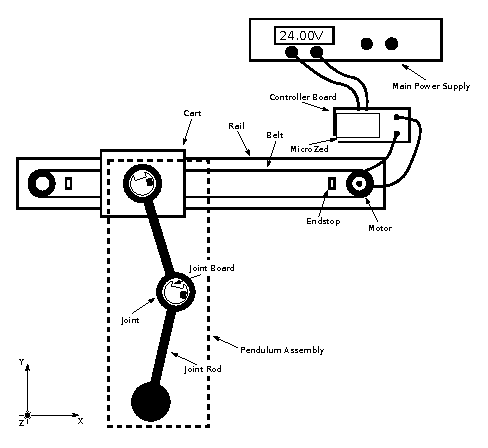
\includegraphics[scale=1.1]{graphics/system_overview}
\end{frame}

\begin{frame}[standout]
  Questions?
\end{frame}

\end{document}